\chapter{Strojenie prostych regulatorów PID i DMC}

\section{Strojenie PID}

Do strojenia wybraliśmy metodę Zieglera-Nicholsa, która rozpoczyna się od doprowadzenia układu do oscylacji krytycznych.

\subsection{Doprowadzenie układu do oscylacji krytycznych}

Wartość $K$, przy której układ osiągnął oscylacji krytycznych to \num{2,78}, $T_{kr} = 7$. 

\begin{figure}[H]
\centering
% This file was created by matlab2tikz.
%
%The latest updates can be retrieved from
%  http://www.mathworks.com/matlabcentral/fileexchange/22022-matlab2tikz-matlab2tikz
%where you can also make suggestions and rate matlab2tikz.
%
\definecolor{mycolor1}{rgb}{0.00000,0.44700,0.74100}%
\definecolor{mycolor2}{rgb}{0.85000,0.32500,0.09800}%
%
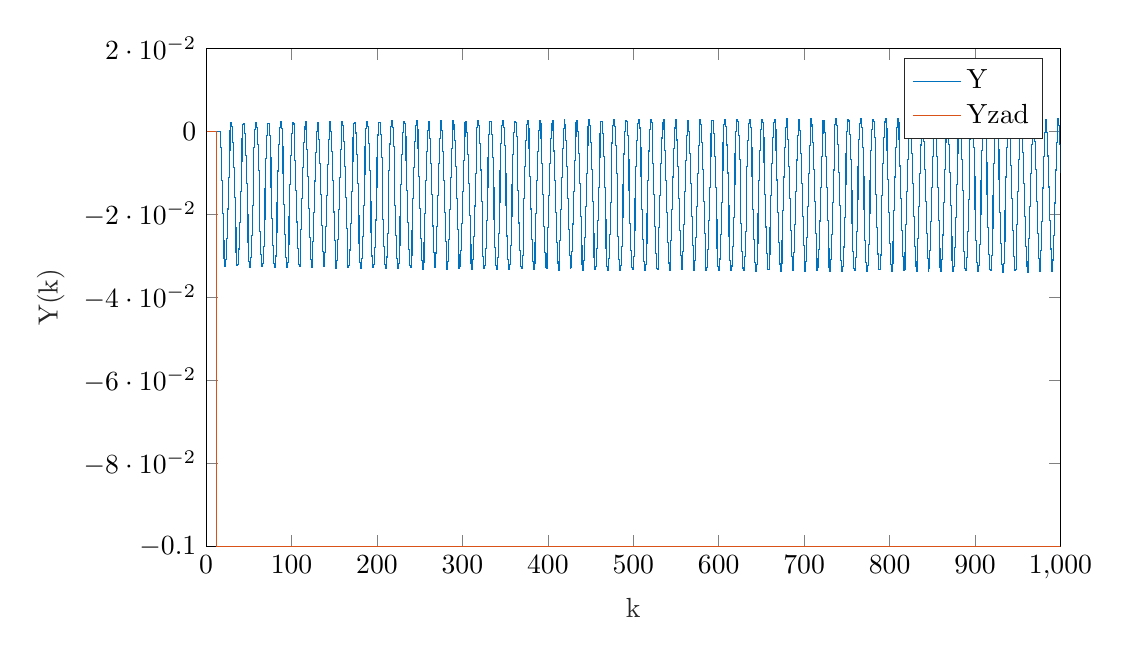
\begin{tikzpicture}

\begin{axis}[%
width=4.272in,
height=2.491in,
at={(0.717in,0.423in)},
scale only axis,
xmin=0,
xmax=1000,
xlabel style={font=\color{white!15!black}},
xlabel={k},
ymin=-0.1,
ymax=0.02,
ylabel style={font=\color{white!15!black}},
ylabel={Y(k)},
axis background/.style={fill=white},
legend style={legend cell align=left, align=left, draw=white!15!black}
]
\addplot[const plot, color=mycolor1] table[row sep=crcr] {%
1	0\\
2	0\\
3	0\\
4	0\\
5	0\\
6	0\\
7	0\\
8	0\\
9	0\\
10	0\\
11	0\\
12	0\\
13	0\\
14	0\\
15	0\\
16	0\\
17	-0.00393323118241956\\
18	-0.0118676283877743\\
19	-0.0198761563606978\\
20	-0.0262811047192933\\
21	-0.0306995619891146\\
22	-0.0325557811637582\\
23	-0.0309170446476251\\
24	-0.0258769815542384\\
25	-0.0187533504928632\\
26	-0.0112041875538502\\
27	-0.00460760223582819\\
28	3.665097427382e-05\\
29	0.00205352538715249\\
30	0.00112426146910821\\
31	-0.00264102429457043\\
32	-0.00867757743247377\\
33	-0.016004594230253\\
34	-0.0233238683663902\\
35	-0.0292052980394042\\
36	-0.0323814113478016\\
37	-0.0320984572393589\\
38	-0.0283844733339248\\
39	-0.0220776562404318\\
40	-0.0145627312327885\\
41	-0.00734436657052908\\
42	-0.00168543577724403\\
43	0.00155481326928456\\
44	0.001927621377024\\
45	-0.000625388545734381\\
46	-0.00575177738008245\\
47	-0.0126633882430605\\
48	-0.0201811742019461\\
49	-0.0268908699845648\\
50	-0.0314069515264772\\
51	-0.0327080926376626\\
52	-0.0304545297346547\\
53	-0.0251398746706121\\
54	-0.0179565690052943\\
55	-0.0104141812317453\\
56	-0.00391906860926718\\
57	0.000481795891266057\\
58	0.00216073171774543\\
59	0.000885852627492215\\
60	-0.00317733541230196\\
61	-0.0094333935124588\\
62	-0.0168626686445075\\
63	-0.0241260695844792\\
64	-0.0297837689791451\\
65	-0.0326067422085118\\
66	-0.0319185706837439\\
67	-0.0278413276993516\\
68	-0.0212954526340749\\
69	-0.0137087231464521\\
70	-0.00658099586127348\\
71	-0.00113834560728369\\
72	0.001805666202099\\
73	0.0018457974666386\\
74	-0.00103223504966468\\
75	-0.00642679752086063\\
76	-0.0134990710049838\\
77	-0.0210291893228627\\
78	-0.0275853709684196\\
79	-0.0317994483945804\\
80	-0.0327076452102958\\
81	-0.0300593065836246\\
82	-0.0244417549371539\\
83	-0.0171112265508389\\
84	-0.00959190721561365\\
85	-0.00326376785896642\\
86	0.000870201568196739\\
87	0.00222684465536822\\
88	0.000617421679734476\\
89	-0.00374557239750481\\
90	-0.0102156004290408\\
91	-0.0177262645062025\\
92	-0.0249090891206116\\
93	-0.0303250398959117\\
94	-0.0327850094136594\\
95	-0.0316901947481406\\
96	-0.0272588089930018\\
97	-0.0204922083146563\\
98	-0.0128550725250403\\
99	-0.00583632319654542\\
100	-0.000622743411829827\\
101	0.00201761383265574\\
102	0.00172277429315783\\
103	-0.00147678209366289\\
104	-0.00712955563308864\\
105	-0.0143465722547516\\
106	-0.0218692378174122\\
107	-0.0282518311184278\\
108	-0.0321482566994591\\
109	-0.0326570297023213\\
110	-0.0296192031948375\\
111	-0.0237143154655481\\
112	-0.0162572072591531\\
113	-0.0087807747252573\\
114	-0.0026349275367795\\
115	0.0012222879652315\\
116	0.00225207354203133\\
117	0.000309058676036262\\
118	-0.00434661004901789\\
119	-0.0110171912634868\\
120	-0.0185908411669134\\
121	-0.0256726230138978\\
122	-0.030828623094638\\
123	-0.0329146084038571\\
124	-0.0314132145848674\\
125	-0.0266392161710545\\
126	-0.01967107310867\\
127	-0.0120043316649849\\
128	-0.00511208752859337\\
129	-0.00013979839836267\\
130	0.00219006618888898\\
131	0.00155873727966624\\
132	-0.00195798800749869\\
133	-0.00785825514237081\\
134	-0.0152035515323273\\
135	-0.0226987677342704\\
136	-0.0288880010630629\\
137	-0.0324520560633874\\
138	-0.0325563385238762\\
139	-0.0291357664903382\\
140	-0.0229600635379727\\
141	-0.0153972045696246\\
142	-0.00798302966511056\\
143	-0.00203407480198285\\
144	0.00153725691182159\\
145	0.00223632462536533\\
146	-3.85820507722861e-05\\
147	-0.00497901008215604\\
148	-0.0118360411265124\\
149	-0.0194538757103356\\
150	-0.0264142206010523\\
151	-0.0312927338409487\\
152	-0.0329949831580846\\
153	-0.0310885654867524\\
154	-0.0259847163318932\\
155	-0.018834747698091\\
156	-0.0111589903734352\\
157	-0.00441013256359829\\
158	0.000309385882674451\\
159	0.00232262366304306\\
160	0.00135400458689251\\
161	-0.00247476034419067\\
162	-0.00861105534320506\\
163	-0.0160676220285918\\
164	-0.0235152391184844\\
165	-0.0294917366642807\\
166	-0.0327097000864885\\
167	-0.0324058526346936\\
168	-0.028610686881586\\
169	-0.0221815588153217\\
170	-0.0145338685311549\\
171	-0.00720081772496805\\
172	-0.0014626266252516\\
173	0.00181440924543905\\
174	0.00217959642245129\\
175	-0.000424754564573031\\
176	-0.00564125245797639\\
177	-0.0126699738969306\\
178	-0.0203128457109016\\
179	-0.0271314989789965\\
180	-0.0317157252560728\\
181	-0.0330257617422132\\
182	-0.0307173562630246\\
183	-0.0252975744207802\\
184	-0.017985926851086\\
185	-0.0103214554735532\\
186	-0.0037321927001809\\
187	0.000723808516681164\\
188	0.00241497953363912\\
189	0.00110898579897851\\
190	-0.00302591914848105\\
191	-0.00938604879829859\\
192	-0.0169363725361997\\
193	-0.0243161483822555\\
194	-0.030061000891744\\
195	-0.0329202101137016\\
196	-0.0322060383730065\\
197	-0.0280457913867563\\
198	-0.0213813997367076\\
199	-0.0136697941397854\\
200	-0.0064361815640023\\
201	-0.000921893328493995\\
202	0.00205314097150422\\
203	0.00208197784443675\\
204	-0.000848623179544481\\
205	-0.00633173926356893\\
206	-0.0135167681532413\\
207	-0.0211652363221938\\
208	-0.0278221502671827\\
209	-0.0320960936366977\\
210	-0.0330067559825079\\
211	-0.0303008607844275\\
212	-0.0245801393650836\\
213	-0.0171272872491502\\
214	-0.00949404560911277\\
215	-0.0030798942415878\\
216	0.00110256776742658\\
217	0.00246691736636704\\
218	0.000824180071015081\\
219	-0.00361019981971958\\
220	-0.0101812661667935\\
221	-0.0178073739488698\\
222	-0.0250990356400817\\
223	-0.030593870383423\\
224	-0.0330827778489284\\
225	-0.0319575426611703\\
226	-0.0274430315794845\\
227	-0.020562209869619\\
228	-0.0128075129212225\\
229	-0.00569105967869156\\
230	-0.000413081598277667\\
231	0.00225294014766129\\
232	0.00194364626895224\\
233	-0.00130926458817018\\
234	-0.00704879855356274\\
235	-0.0143741629149044\\
236	-0.0220085472765619\\
237	-0.0284839487289901\\
238	-0.0324324832656335\\
239	-0.0329379602775064\\
240	-0.0298405088480369\\
241	-0.0238348303533007\\
242	-0.0162614762925332\\
243	-0.00867898715573742\\
244	-0.00245475717514231\\
245	0.00144485766465879\\
246	0.0024783086831566\\
247	0.000500174406987883\\
248	-0.00422625600305956\\
249	-0.0109946810599129\\
250	-0.0186781857089613\\
251	-0.0258614918942701\\
252	-0.0310885416447447\\
253	-0.033196767274091\\
254	-0.0316611874064476\\
255	-0.0268044712571491\\
256	-0.0197266248984345\\
257	-0.0119494856501074\\
258	-0.00496728611313112\\
259	6.27023178690363e-05\\
260	0.00241338400566303\\
261	0.00176486583030082\\
262	-0.00180566996739752\\
263	-0.0077906882419989\\
264	-0.0152398633749558\\
265	-0.0228402997941383\\
266	-0.0291147576594017\\
267	-0.0327236906905464\\
268	-0.032819549604761\\
269	-0.0293378764520412\\
270	-0.0230641233432223\\
271	-0.0153911019038026\\
272	-0.00787841116811319\\
273	-0.00185819741090892\\
274	0.00174996470760536\\
275	0.0024491109046962\\
276	0.000137642042076158\\
277	-0.0048726625243892\\
278	-0.0118242149271128\\
279	-0.0195463622101934\\
280	-0.0266011660775859\\
281	-0.0315433368779263\\
282	-0.0332617158654656\\
283	-0.0313179631400951\\
284	-0.026132273929498\\
285	-0.0188772803238342\\
286	-0.0110980961725226\\
287	-0.00426659090372404\\
288	0.000504449326173151\\
289	0.00253413633848017\\
290	0.00154598590608628\\
291	-0.00233674708500917\\
292	-0.00855560005050187\\
293	-0.0161115466288948\\
294	-0.0236580434106422\\
295	-0.0297125360372245\\
296	-0.032968668456105\\
297	-0.0326518767354777\\
298	-0.0287946755592885\\
299	-0.0222705378959615\\
300	-0.0145187233452232\\
301	-0.00709435127918074\\
302	-0.00129152937157985\\
303	0.00201726474106369\\
304	0.00237936555962846\\
305	-0.000262659098015816\\
306	-0.00554791838173261\\
307	-0.0126677419763901\\
308	-0.0204094591640491\\
309	-0.0273157719579017\\
310	-0.0319567094291037\\
311	-0.0332773350995927\\
312	-0.0309290219418998\\
313	-0.0254286902263027\\
314	-0.0180167999328217\\
315	-0.0102556462867523\\
316	-0.00359060115128731\\
317	0.00091124419537853\\
318	0.00261494516922719\\
319	0.00128743977479567\\
320	-0.00290132242742877\\
321	-0.00934166351848323\\
322	-0.0169868674059329\\
323	-0.0244593627325484\\
324	-0.0302753449364861\\
325	-0.0331665282727835\\
326	-0.0324354686731054\\
327	-0.0282127434304528\\
328	-0.0214566244242014\\
329	-0.0136468430520615\\
330	-0.00632874246261806\\
331	-0.000755968833044193\\
332	0.00224622004885381\\
333	0.00226919674635405\\
334	-0.000699887888504937\\
335	-0.00625044980477037\\
336	-0.0135230941331209\\
337	-0.0212650399387252\\
338	-0.0280030949069792\\
339	-0.0323272488373394\\
340	-0.0332435102418974\\
341	-0.0304956697013229\\
342	-0.0246960453197721\\
343	-0.0171477850864824\\
344	-0.00942435162771194\\
345	-0.00294084261626071\\
346	0.00128226233157773\\
347	0.00265564070856406\\
348	0.000989743415911512\\
349	-0.00349814336892748\\
350	-0.0101469500809106\\
351	-0.0178634638095222\\
352	-0.0252418841267744\\
353	-0.0308013536877892\\
354	-0.0333165436039997\\
355	-0.0321710223355139\\
356	-0.0275940316092842\\
357	-0.0206249519341786\\
358	-0.012777899471519\\
359	-0.00558342056709894\\
360	-0.000252635923360155\\
361	0.00243637669810699\\
362	0.00211880982739085\\
363	-0.00117312147526576\\
364	-0.00697861339298166\\
365	-0.014388066042423\\
366	-0.0221106818792825\\
367	-0.0286609985323161\\
368	-0.0326536854662922\\
369	-0.0331602994127173\\
370	-0.030019357770476\\
371	-0.0239367264537658\\
372	-0.0162728048603514\\
373	-0.00860633849259116\\
374	-0.00231874173670701\\
375	0.00161676668018402\\
376	0.00265613359844158\\
377	0.000653494422294866\\
378	-0.00412588040065026\\
379	-0.0109694772189982\\
380	-0.0187389630745903\\
381	-0.02600328235006\\
382	-0.0312888457764584\\
383	-0.0334181516523398\\
384	-0.0318593995044963\\
385	-0.026940594643498\\
386	-0.0197780963317031\\
387	-0.0119142608858075\\
388	-0.00486012252966475\\
389	0.000217441803328048\\
390	0.00258736215731462\\
391	0.0019284903315064\\
392	-0.00168135674943574\\
393	-0.00773069934176647\\
394	-0.0152604201205303\\
395	-0.0229439826169466\\
396	-0.0292874311674397\\
397	-0.0329348946964037\\
398	-0.0330279319277543\\
399	-0.0295016740681717\\
400	-0.0231531706674637\\
401	-0.0153943870604617\\
402	-0.00780364153904905\\
403	-0.00172562797390574\\
404	0.00191410480538469\\
405	0.00261641343243065\\
406	0.000279370993722935\\
407	-0.00478312943614895\\
408	-0.0118072126890262\\
409	-0.019610987349066\\
410	-0.026741287120754\\
411	-0.0317362244604051\\
412	-0.033470954725412\\
413	-0.0315016210708725\\
414	-0.0262545786253488\\
415	-0.0189186293530272\\
416	-0.0110582201879309\\
417	-0.00416048717588163\\
418	0.000653326292223707\\
419	0.00269888320136059\\
420	0.00169860303529382\\
421	-0.00222351185203614\\
422	-0.00850493476481598\\
423	-0.0161378916610272\\
424	-0.0237625663743268\\
425	-0.0298804322122347\\
426	-0.0331699006530103\\
427	-0.0328468059130196\\
428	-0.0289443336981426\\
429	-0.0223478527960564\\
430	-0.0145150101269021\\
431	-0.00701820228264922\\
432	-0.00116273639633525\\
433	0.00217370618706981\\
434	0.00253654753641053\\
435	-0.000131869019548986\\
436	-0.00546841420829031\\
437	-0.0126580788343772\\
438	-0.0204771595070948\\
439	-0.0274536896328406\\
440	-0.032142018086888\\
441	-0.0334747209624418\\
442	-0.0310988606083525\\
443	-0.0255382096357607\\
444	-0.0180491081717219\\
445	-0.0102119905700666\\
446	-0.00348605651608339\\
447	0.00105416597763842\\
448	0.00277072410797394\\
449	0.00142959119340488\\
450	-0.00279842773195124\\
451	-0.00929948711999115\\
452	-0.0170181940019873\\
453	-0.0245640902716892\\
454	-0.0304381383109504\\
455	-0.0333578794439316\\
456	-0.0326174851981076\\
457	-0.028349169148089\\
458	-0.0215232738252927\\
459	-0.0136370959261259\\
460	-0.00625186831702132\\
461	-0.000631210419513934\\
462	0.00239507976538245\\
463	0.00241667998806283\\
464	-0.000579389053634291\\
465	-0.00618018877057647\\
466	-0.0135199569857716\\
467	-0.0213351090008017\\
468	-0.0281383490088115\\
469	-0.0325048850838766\\
470	-0.0334293844040914\\
471	-0.0306524373144285\\
472	-0.0247937821749795\\
473	-0.0171720657229962\\
474	-0.00937770207700987\\
475	-0.00283827744974023\\
476	0.0014191928927416\\
477	0.00280274514220371\\
478	0.00112197588518187\\
479	-0.00340486977855706\\
480	-0.0101124677450705\\
481	-0.0178990237600784\\
482	-0.0253462506373759\\
483	-0.0309587893515592\\
484	-0.0334981618788912\\
485	-0.0323406954960355\\
486	-0.0277181201393682\\
487	-0.0206819496703741\\
488	-0.0127630034233942\\
489	-0.00550639317836492\\
490	-0.000132104626347661\\
491	0.00257781175378328\\
492	0.00225703084937909\\
493	-0.00106227477743049\\
494	-0.00691684011414215\\
495	-0.0143906919545831\\
496	-0.0221824777565647\\
497	-0.0287931986844984\\
498	-0.0328236185986365\\
499	-0.033335044390184\\
500	-0.0301638083617806\\
501	-0.0240236476610476\\
502	-0.0162900017772212\\
503	-0.00855739897095485\\
504	-0.00221850379366805\\
505	0.00174771994578874\\
506	0.00279488131866353\\
507	0.000776355444839871\\
508	-0.00404152954808663\\
509	-0.0109419355089414\\
510	-0.0187780661375187\\
511	-0.0261067893230466\\
512	-0.0314407342662342\\
513	-0.0335902356426766\\
514	-0.0320173198828596\\
515	-0.0270532231997769\\
516	-0.0198264004428021\\
517	-0.0118950232176722\\
518	-0.00478343677524308\\
519	0.000333612399855062\\
520	0.00272156373294304\\
521	0.00205789558318676\\
522	-0.0015795350760337\\
523	-0.00767669091002095\\
524	-0.0152680966239951\\
525	-0.0230169261205293\\
526	-0.0294162527152977\\
527	-0.0330971507535519\\
528	-0.0331919642730085\\
529	-0.0296345607088645\\
530	-0.023230203074945\\
531	-0.0154053747848929\\
532	-0.00775303784888249\\
533	-0.00162799855425303\\
534	0.00203913840039489\\
535	0.00274714142540973\\
536	0.000393404942520183\\
537	-0.00470702660056162\\
538	-0.0117859005831411\\
539	-0.0196530003073699\\
540	-0.0268435000216708\\
541	-0.0318824366089635\\
542	-0.0336337468942689\\
543	-0.0316483935957104\\
544	-0.0263566010338803\\
545	-0.0189591402614448\\
546	-0.0110353729130851\\
547	-0.00408456630503485\\
548	0.000765055289815831\\
549	0.00282607102991654\\
550	0.00181964462245085\\
551	-0.0021301030965189\\
552	-0.00845800238474041\\
553	-0.0161499566425946\\
554	-0.0238361388565173\\
555	-0.0300056119894257\\
556	-0.0333245564871581\\
557	-0.033000569437649\\
558	-0.0290664024233561\\
559	-0.0224158798279861\\
560	-0.0145205945059911\\
561	-0.00696648644996539\\
562	-0.00106793636895513\\
563	0.00229291558884872\\
564	0.00265960728840101\\
565	-2.61243156422046e-05\\
566	-0.00539991046187834\\
567	-0.0126423283380872\\
568	-0.0205215048820283\\
569	-0.0275542345831756\\
570	-0.0322824798828458\\
571	-0.0336285012653247\\
572	-0.0312350981736698\\
573	-0.0256304517666353\\
574	-0.0180826676563577\\
575	-0.0101861932936956\\
576	-0.00341125757979278\\
577	0.00116141920248457\\
578	0.00289114137996358\\
579	0.0015427230597469\\
580	-0.00271283737915632\\
581	-0.00925897733593277\\
582	-0.0170340352247711\\
583	-0.0246378311975905\\
584	-0.0305594703300223\\
585	-0.0335050569469594\\
586	-0.0327614446252673\\
587	-0.0284611535768323\\
588	-0.0215831329230389\\
589	-0.0136380154277558\\
590	-0.00619952308761969\\
591	-0.000539406047950373\\
592	0.00250859287931332\\
593	0.00253243325150215\\
594	-0.0004814052989382\\
595	-0.00611866272347647\\
596	-0.0135091433678642\\
597	-0.0213812634689016\\
598	-0.0282369093193972\\
599	-0.0326395725864705\\
600	-0.0335744642333595\\
601	-0.0307787549719084\\
602	-0.0248770381365515\\
603	-0.0171994566058947\\
604	-0.00934954526193352\\
605	-0.00276489668648133\\
606	0.00152197728353828\\
607	0.00291665386207526\\
608	0.00122765042372409\\
609	-0.0033265230947071\\
610	-0.0100777632934482\\
611	-0.0179180780619662\\
612	-0.0254197549503348\\
613	-0.0310761204641506\\
614	-0.0336380223999102\\
615	-0.0324753305603833\\
616	-0.0278207367733187\\
617	-0.0207344304763641\\
618	-0.0127599309664094\\
619	-0.00545383663906954\\
620	-4.34131527511579e-05\\
621	0.00268578391010267\\
622	0.00236584584390623\\
623	-0.000971535803707276\\
624	-0.00686169928998706\\
625	-0.0143842336470258\\
626	-0.0222299703161356\\
627	-0.0288895112865629\\
628	-0.0329525529460941\\
629	-0.0334717608477776\\
630	-0.0302808180855773\\
631	-0.0240986767142858\\
632	-0.0163119482394675\\
633	-0.00852740749548318\\
634	-0.00214678190953448\\
635	0.00184607830505117\\
636	0.00290255809376531\\
637	0.000875020509508094\\
638	-0.00396987340596098\\
639	-0.0109124558304275\\
640	-0.0187998183483742\\
641	-0.0261797046484598\\
642	-0.0315539598331034\\
643	-0.0337229746264917\\
644	-0.0321431198888692\\
645	-0.0271471673780249\\
646	-0.0198722436614167\\
647	-0.0118885684403609\\
648	-0.00473102702446908\\
649	0.000419117445097029\\
650	0.00282417309710775\\
651	0.00216014360460534\\
652	-0.00149553907177011\\
653	-0.00762737278338905\\
654	-0.015265454822507\\
655	-0.023065336049872\\
656	-0.0295101045299906\\
657	-0.0332203932981315\\
658	-0.0333206747904774\\
659	-0.0297428667259584\\
660	-0.0232977272213474\\
661	-0.0154225432300562\\
662	-0.00772167477281808\\
663	-0.00155812584726795\\
664	0.00213314451573023\\
665	0.00284887366598313\\
666	0.000485501230724105\\
667	-0.0046415309692233\\
668	-0.0117611020279266\\
669	-0.0196769819241119\\
670	-0.0269155237495853\\
671	-0.0319914962150022\\
672	-0.0337595887651547\\
673	-0.0317658524394716\\
674	-0.0264425435155933\\
675	-0.0189990371298891\\
676	-0.0110260847950314\\
677	-0.0040326061076787\\
678	0.000847339075698922\\
679	0.00292351441391506\\
680	0.00191569703208365\\
681	-0.00205236449993954\\
682	-0.00841397511052382\\
683	-0.0161506346433905\\
684	-0.0238850935028746\\
685	-0.0300968362721064\\
686	-0.0334422040848793\\
687	-0.0331216467570952\\
688	-0.0291665970971794\\
689	-0.0224765820214759\\
690	-0.0145335948923686\\
691	-0.00693415691385588\\
692	-0.00100005765781438\\
693	0.00238266972389737\\
694	0.00275568979509869\\
695	5.98344620685272e-05\\
696	-0.00534006958908258\\
697	-0.0126217040959684\\
698	-0.0205472925381165\\
699	-0.0276251108661578\\
700	-0.0323873531275387\\
701	-0.0337476945755392\\
702	-0.0313447098280951\\
703	-0.0257090359094154\\
704	-0.0181172599586735\\
705	-0.010174563052676\\
706	-0.00335999895163947\\
707	0.0012404808967848\\
708	0.00298363043824712\\
709	0.00163294862667126\\
710	-0.00264088846239907\\
711	-0.00921974019933851\\
712	-0.0170375775309017\\
713	-0.0246870036324658\\
714	-0.0306479430213072\\
715	-0.0336172374254161\\
716	-0.0328752721499729\\
717	-0.0285538138272457\\
718	-0.0216376558542709\\
719	-0.0136474029944724\\
720	-0.00616657827936153\\
721	-0.000473625374829182\\
722	0.00259421762850518\\
723	0.00262316516577157\\
724	-0.00040116415697859\\
725	-0.00606399603754704\\
726	-0.0134922231533077\\
727	-0.0214084772320962\\
728	-0.0283064260183298\\
729	-0.0327402749759414\\
730	-0.03368727709133\\
731	-0.0308810094306776\\
732	-0.0249488776349492\\
733	-0.0172293371644004\\
734	-0.00933600945450534\\
735	-0.00271454536286125\\
736	0.00159784567132078\\
737	0.00300441165308227\\
738	0.00131241299291588\\
739	-0.00325991526519458\\
740	-0.0100428469079528\\
741	-0.0179240692905895\\
742	-0.0254688615235702\\
743	-0.0311617565757094\\
744	-0.033744890223359\\
745	-0.0325822980795595\\
746	-0.027906421012105\\
747	-0.0207833758768261\\
748	-0.012766208282902\\
749	-0.00542057777072858\\
750	2.02017618404736e-05\\
751	0.00276742040695574\\
752	0.00245152793612679\\
753	-0.000896605484711071\\
754	-0.00681175204655892\\
755	-0.0143705831677062\\
756	-0.0222582718457097\\
757	-0.0289574968933947\\
758	-0.0330491319089168\\
759	-0.0335784766368467\\
760	-0.0303761977571313\\
761	-0.0241643538604373\\
762	-0.0163376618198594\\
763	-0.00851235125706373\\
764	-0.00209750166176167\\
765	0.001918807727574\\
766	0.00298581598619517\\
767	0.000954676969824295\\
768	-0.00390817824954799\\
769	-0.0108814221095671\\
770	-0.018807881968154\\
771	-0.0262285024702854\\
772	-0.0316367098924782\\
773	-0.0338247067736098\\
774	-0.0322436196771\\
775	-0.0272264129358074\\
776	-0.0199161720745061\\
777	-0.0118921877137578\\
778	-0.00469770927057729\\
779	0.000480531010099881\\
780	0.0029019775623944\\
781	0.00224107587497499\\
782	-0.00142552723119601\\
783	-0.00758171648101242\\
784	-0.0152546750580957\\
785	-0.0230944266417942\\
786	-0.0295764250930532\\
787	-0.033312924343489\\
788	-0.0334215881854727\\
789	-0.0298318432653612\\
790	-0.023357791647952\\
791	-0.0154445877990461\\
792	-0.00770543514021668\\
793	-0.00151004261839267\\
794	0.00220281112604057\\
795	0.00292786856790915\\
796	0.000560399757824028\\
797	-0.00458434105822814\\
798	-0.0117335439553359\\
799	-0.0196867788497744\\
800	-0.0269638081268151\\
801	-0.0320713427903183\\
802	-0.033856380831447\\
803	-0.031860275728\\
804	-0.026515864533447\\
805	-0.019038468096677\\
806	-0.0110274503752509\\
807	-0.00399944246418278\\
808	0.000906543908294256\\
809	0.00299765502751685\\
810	0.00199217659979691\\
811	-0.00198689442648084\\
812	-0.00837220769772453\\
813	-0.0161423609596274\\
814	-0.0239147120488778\\
815	-0.0301613923464301\\
816	-0.0335307871184044\\
817	-0.033217060042742\\
818	-0.0292496286606681\\
819	-0.0225315498862653\\
820	-0.0145524231699297\\
821	-0.00691702618026468\\
822	-0.000953263496404852\\
823	0.00244936805139885\\
824	0.0028306616835623\\
825	0.000130313012715688\\
826	-0.00528699907685517\\
827	-0.0125972453166056\\
828	-0.0205585196070513\\
829	-0.027672712715824\\
830	-0.0324643074498722\\
831	-0.0338397571093168\\
832	-0.0314334436420828\\
833	-0.0257769216663758\\
834	-0.0181526725672478\\
835	-0.0101740340805877\\
836	-0.00332716398204406\\
837	0.00129749417517268\\
838	0.00305428451679086\\
839	0.00170526788380756\\
840	-0.00257960002327678\\
841	-0.00918148609434794\\
842	-0.0170314786522305\\
843	-0.0247169245164034\\
844	-0.0307106666634368\\
845	-0.0337019932351301\\
846	-0.0329654918422843\\
847	-0.0286313427317539\\
848	-0.0216880094246777\\
849	-0.013663424246393\\
850	-0.00614880733862043\\
851	-0.000428182151854725\\
852	0.00265805744163346\\
853	0.0026943548945587\\
854	-0.00033477912134198\\
855	-0.00601468105980507\\
856	-0.0134705174073264\\
857	-0.0214208655857707\\
858	-0.028353209279345\\
859	-0.0328143736743022\\
860	-0.0337748321694486\\
861	-0.0309644337839271\\
862	-0.0250117912810892\\
863	-0.0172611709134021\\
864	-0.00933390260409388\\
865	-0.00268217880487122\\
866	0.00165270575998258\\
867	0.00307176311438421\\
868	0.00138085800057078\\
869	-0.00320246565186443\\
870	-0.0100077568509697\\
871	-0.0179198461528981\\
872	-0.025498892476062\\
873	-0.0312226083998374\\
874	-0.0338259571455129\\
875	-0.0326676318487739\\
876	-0.0279788717799386\\
877	-0.0208295634736641\\
878	-0.0127797903032932\\
879	-0.00540237941416649\\
880	6.42588624029863e-05\\
881	0.00282852386073211\\
882	0.00251917529988183\\
883	-0.000834000065732852\\
884	-0.00676585094835626\\
885	-0.0143513135869787\\
886	-0.0222715852366176\\
887	-0.0290033559543262\\
888	-0.0331204338702835\\
889	-0.0336617546839591\\
890	-0.0304546831934574\\
891	-0.0242227315241392\\
892	-0.0163663177490045\\
893	-0.00850894352809036\\
894	-0.00206571187385624\\
895	0.00197157106984547\\
896	0.00305005308103043\\
897	0.00101952607529069\\
898	-0.00385424254247552\\
899	-0.0108491728660978\\
900	-0.0188052664714511\\
901	-0.026258482400387\\
902	-0.0316956762022768\\
903	-0.0339022375459046\\
904	-0.0323243735684588\\
905	-0.0272941907029416\\
906	-0.0199586083340742\\
907	-0.0119036589513158\\
908	-0.00467926140582811\\
909	0.000523190231540763\\
910	0.00296047661593951\\
911	0.00230541790856773\\
912	-0.00136640097184711\\
913	-0.00753890988689439\\
914	-0.0152375533439546\\
915	-0.0231084596846829\\
916	-0.0296212822517764\\
917	-0.0333815077080755\\
918	-0.0335008250383755\\
919	-0.029905748733821\\
920	-0.0234120418854065\\
921	-0.0154704298419748\\
922	-0.00770096666331731\\
923	-0.00147890985124936\\
924	0.00225354939589582\\
925	0.00298918185956738\\
926	0.000621922412996096\\
927	-0.00453361262799831\\
928	-0.0117038378878866\\
929	-0.0196855325289701\\
930	-0.0269936049473182\\
931	-0.0321284327986577\\
932	-0.0339305396390363\\
933	-0.0319367516746549\\
934	-0.0265793537985807\\
935	-0.0190775345117256\\
936	-0.0110371021613516\\
937	-0.00398089123103242\\
938	0.000947813892891596\\
939	0.00305368911550391\\
940	0.00205344609284038\\
941	-0.00193096101741313\\
942	-0.00833219844138068\\
943	-0.0161271264589977\\
944	-0.0239292884331198\\
945	-0.0302051953153232\\
946	-0.0335967464183303\\
947	-0.0332924942594718\\
948	-0.0293192997101761\\
949	-0.0225820534410466\\
950	-0.0145757796875602\\
951	-0.00691170300166095\\
952	-0.0009228429789353\\
953	0.00249816555408913\\
954	0.00288924225596257\\
955	0.000188768775298753\\
956	-0.00523918983756799\\
957	-0.0125698098407712\\
958	-0.0205584322373984\\
959	-0.0277022211768241\\
960	-0.0325195505966457\\
961	-0.0339107168271545\\
962	-0.0315059372626552\\
963	-0.0258364853568901\\
964	-0.018188718268643\\
965	-0.0101821229215982\\
966	-0.00330862674554909\\
967	0.00133740116456837\\
968	0.00310799845821128\\
969	0.00176369209136024\\
970	-0.0025265878535639\\
971	-0.00914399902289456\\
972	-0.0170178973479614\\
973	-0.0247318951946017\\
974	-0.0307533861318656\\
975	-0.0337654366828833\\
976	-0.0330373622538972\\
977	-0.028697110009198\\
978	-0.0217351192654272\\
979	-0.0136845897020041\\
980	-0.00614280415660312\\
981	-0.000398506985834209\\
982	0.00270500875115781\\
983	0.00275039277029162\\
984	-0.00027914142082677\\
985	-0.00596952158947854\\
986	-0.0134451043471365\\
987	-0.0214217537379848\\
988	-0.0283823488228985\\
989	-0.0328678170508264\\
990	-0.0338427718029049\\
991	-0.0310332324556903\\
992	-0.0250677701113869\\
993	-0.0172945136560273\\
994	-0.0093406525045531\\
995	-0.00266374701068417\\
996	0.00169129101869666\\
997	0.00312330524180586\\
998	0.00143665753228614\\
999	-0.00315211821905617\\
1000	-0.00997253851788046\\
};
\addlegendentry{Y}

\addplot[const plot, color=mycolor2] table[row sep=crcr] {%
1	0\\
2	0\\
3	0\\
4	0\\
5	0\\
6	0\\
7	0\\
8	0\\
9	0\\
10	0\\
11	0\\
12	-0.1\\
13	-0.1\\
14	-0.1\\
15	-0.1\\
16	-0.1\\
17	-0.1\\
18	-0.1\\
19	-0.1\\
20	-0.1\\
21	-0.1\\
22	-0.1\\
23	-0.1\\
24	-0.1\\
25	-0.1\\
26	-0.1\\
27	-0.1\\
28	-0.1\\
29	-0.1\\
30	-0.1\\
31	-0.1\\
32	-0.1\\
33	-0.1\\
34	-0.1\\
35	-0.1\\
36	-0.1\\
37	-0.1\\
38	-0.1\\
39	-0.1\\
40	-0.1\\
41	-0.1\\
42	-0.1\\
43	-0.1\\
44	-0.1\\
45	-0.1\\
46	-0.1\\
47	-0.1\\
48	-0.1\\
49	-0.1\\
50	-0.1\\
51	-0.1\\
52	-0.1\\
53	-0.1\\
54	-0.1\\
55	-0.1\\
56	-0.1\\
57	-0.1\\
58	-0.1\\
59	-0.1\\
60	-0.1\\
61	-0.1\\
62	-0.1\\
63	-0.1\\
64	-0.1\\
65	-0.1\\
66	-0.1\\
67	-0.1\\
68	-0.1\\
69	-0.1\\
70	-0.1\\
71	-0.1\\
72	-0.1\\
73	-0.1\\
74	-0.1\\
75	-0.1\\
76	-0.1\\
77	-0.1\\
78	-0.1\\
79	-0.1\\
80	-0.1\\
81	-0.1\\
82	-0.1\\
83	-0.1\\
84	-0.1\\
85	-0.1\\
86	-0.1\\
87	-0.1\\
88	-0.1\\
89	-0.1\\
90	-0.1\\
91	-0.1\\
92	-0.1\\
93	-0.1\\
94	-0.1\\
95	-0.1\\
96	-0.1\\
97	-0.1\\
98	-0.1\\
99	-0.1\\
100	-0.1\\
101	-0.1\\
102	-0.1\\
103	-0.1\\
104	-0.1\\
105	-0.1\\
106	-0.1\\
107	-0.1\\
108	-0.1\\
109	-0.1\\
110	-0.1\\
111	-0.1\\
112	-0.1\\
113	-0.1\\
114	-0.1\\
115	-0.1\\
116	-0.1\\
117	-0.1\\
118	-0.1\\
119	-0.1\\
120	-0.1\\
121	-0.1\\
122	-0.1\\
123	-0.1\\
124	-0.1\\
125	-0.1\\
126	-0.1\\
127	-0.1\\
128	-0.1\\
129	-0.1\\
130	-0.1\\
131	-0.1\\
132	-0.1\\
133	-0.1\\
134	-0.1\\
135	-0.1\\
136	-0.1\\
137	-0.1\\
138	-0.1\\
139	-0.1\\
140	-0.1\\
141	-0.1\\
142	-0.1\\
143	-0.1\\
144	-0.1\\
145	-0.1\\
146	-0.1\\
147	-0.1\\
148	-0.1\\
149	-0.1\\
150	-0.1\\
151	-0.1\\
152	-0.1\\
153	-0.1\\
154	-0.1\\
155	-0.1\\
156	-0.1\\
157	-0.1\\
158	-0.1\\
159	-0.1\\
160	-0.1\\
161	-0.1\\
162	-0.1\\
163	-0.1\\
164	-0.1\\
165	-0.1\\
166	-0.1\\
167	-0.1\\
168	-0.1\\
169	-0.1\\
170	-0.1\\
171	-0.1\\
172	-0.1\\
173	-0.1\\
174	-0.1\\
175	-0.1\\
176	-0.1\\
177	-0.1\\
178	-0.1\\
179	-0.1\\
180	-0.1\\
181	-0.1\\
182	-0.1\\
183	-0.1\\
184	-0.1\\
185	-0.1\\
186	-0.1\\
187	-0.1\\
188	-0.1\\
189	-0.1\\
190	-0.1\\
191	-0.1\\
192	-0.1\\
193	-0.1\\
194	-0.1\\
195	-0.1\\
196	-0.1\\
197	-0.1\\
198	-0.1\\
199	-0.1\\
200	-0.1\\
201	-0.1\\
202	-0.1\\
203	-0.1\\
204	-0.1\\
205	-0.1\\
206	-0.1\\
207	-0.1\\
208	-0.1\\
209	-0.1\\
210	-0.1\\
211	-0.1\\
212	-0.1\\
213	-0.1\\
214	-0.1\\
215	-0.1\\
216	-0.1\\
217	-0.1\\
218	-0.1\\
219	-0.1\\
220	-0.1\\
221	-0.1\\
222	-0.1\\
223	-0.1\\
224	-0.1\\
225	-0.1\\
226	-0.1\\
227	-0.1\\
228	-0.1\\
229	-0.1\\
230	-0.1\\
231	-0.1\\
232	-0.1\\
233	-0.1\\
234	-0.1\\
235	-0.1\\
236	-0.1\\
237	-0.1\\
238	-0.1\\
239	-0.1\\
240	-0.1\\
241	-0.1\\
242	-0.1\\
243	-0.1\\
244	-0.1\\
245	-0.1\\
246	-0.1\\
247	-0.1\\
248	-0.1\\
249	-0.1\\
250	-0.1\\
251	-0.1\\
252	-0.1\\
253	-0.1\\
254	-0.1\\
255	-0.1\\
256	-0.1\\
257	-0.1\\
258	-0.1\\
259	-0.1\\
260	-0.1\\
261	-0.1\\
262	-0.1\\
263	-0.1\\
264	-0.1\\
265	-0.1\\
266	-0.1\\
267	-0.1\\
268	-0.1\\
269	-0.1\\
270	-0.1\\
271	-0.1\\
272	-0.1\\
273	-0.1\\
274	-0.1\\
275	-0.1\\
276	-0.1\\
277	-0.1\\
278	-0.1\\
279	-0.1\\
280	-0.1\\
281	-0.1\\
282	-0.1\\
283	-0.1\\
284	-0.1\\
285	-0.1\\
286	-0.1\\
287	-0.1\\
288	-0.1\\
289	-0.1\\
290	-0.1\\
291	-0.1\\
292	-0.1\\
293	-0.1\\
294	-0.1\\
295	-0.1\\
296	-0.1\\
297	-0.1\\
298	-0.1\\
299	-0.1\\
300	-0.1\\
301	-0.1\\
302	-0.1\\
303	-0.1\\
304	-0.1\\
305	-0.1\\
306	-0.1\\
307	-0.1\\
308	-0.1\\
309	-0.1\\
310	-0.1\\
311	-0.1\\
312	-0.1\\
313	-0.1\\
314	-0.1\\
315	-0.1\\
316	-0.1\\
317	-0.1\\
318	-0.1\\
319	-0.1\\
320	-0.1\\
321	-0.1\\
322	-0.1\\
323	-0.1\\
324	-0.1\\
325	-0.1\\
326	-0.1\\
327	-0.1\\
328	-0.1\\
329	-0.1\\
330	-0.1\\
331	-0.1\\
332	-0.1\\
333	-0.1\\
334	-0.1\\
335	-0.1\\
336	-0.1\\
337	-0.1\\
338	-0.1\\
339	-0.1\\
340	-0.1\\
341	-0.1\\
342	-0.1\\
343	-0.1\\
344	-0.1\\
345	-0.1\\
346	-0.1\\
347	-0.1\\
348	-0.1\\
349	-0.1\\
350	-0.1\\
351	-0.1\\
352	-0.1\\
353	-0.1\\
354	-0.1\\
355	-0.1\\
356	-0.1\\
357	-0.1\\
358	-0.1\\
359	-0.1\\
360	-0.1\\
361	-0.1\\
362	-0.1\\
363	-0.1\\
364	-0.1\\
365	-0.1\\
366	-0.1\\
367	-0.1\\
368	-0.1\\
369	-0.1\\
370	-0.1\\
371	-0.1\\
372	-0.1\\
373	-0.1\\
374	-0.1\\
375	-0.1\\
376	-0.1\\
377	-0.1\\
378	-0.1\\
379	-0.1\\
380	-0.1\\
381	-0.1\\
382	-0.1\\
383	-0.1\\
384	-0.1\\
385	-0.1\\
386	-0.1\\
387	-0.1\\
388	-0.1\\
389	-0.1\\
390	-0.1\\
391	-0.1\\
392	-0.1\\
393	-0.1\\
394	-0.1\\
395	-0.1\\
396	-0.1\\
397	-0.1\\
398	-0.1\\
399	-0.1\\
400	-0.1\\
401	-0.1\\
402	-0.1\\
403	-0.1\\
404	-0.1\\
405	-0.1\\
406	-0.1\\
407	-0.1\\
408	-0.1\\
409	-0.1\\
410	-0.1\\
411	-0.1\\
412	-0.1\\
413	-0.1\\
414	-0.1\\
415	-0.1\\
416	-0.1\\
417	-0.1\\
418	-0.1\\
419	-0.1\\
420	-0.1\\
421	-0.1\\
422	-0.1\\
423	-0.1\\
424	-0.1\\
425	-0.1\\
426	-0.1\\
427	-0.1\\
428	-0.1\\
429	-0.1\\
430	-0.1\\
431	-0.1\\
432	-0.1\\
433	-0.1\\
434	-0.1\\
435	-0.1\\
436	-0.1\\
437	-0.1\\
438	-0.1\\
439	-0.1\\
440	-0.1\\
441	-0.1\\
442	-0.1\\
443	-0.1\\
444	-0.1\\
445	-0.1\\
446	-0.1\\
447	-0.1\\
448	-0.1\\
449	-0.1\\
450	-0.1\\
451	-0.1\\
452	-0.1\\
453	-0.1\\
454	-0.1\\
455	-0.1\\
456	-0.1\\
457	-0.1\\
458	-0.1\\
459	-0.1\\
460	-0.1\\
461	-0.1\\
462	-0.1\\
463	-0.1\\
464	-0.1\\
465	-0.1\\
466	-0.1\\
467	-0.1\\
468	-0.1\\
469	-0.1\\
470	-0.1\\
471	-0.1\\
472	-0.1\\
473	-0.1\\
474	-0.1\\
475	-0.1\\
476	-0.1\\
477	-0.1\\
478	-0.1\\
479	-0.1\\
480	-0.1\\
481	-0.1\\
482	-0.1\\
483	-0.1\\
484	-0.1\\
485	-0.1\\
486	-0.1\\
487	-0.1\\
488	-0.1\\
489	-0.1\\
490	-0.1\\
491	-0.1\\
492	-0.1\\
493	-0.1\\
494	-0.1\\
495	-0.1\\
496	-0.1\\
497	-0.1\\
498	-0.1\\
499	-0.1\\
500	-0.1\\
501	-0.1\\
502	-0.1\\
503	-0.1\\
504	-0.1\\
505	-0.1\\
506	-0.1\\
507	-0.1\\
508	-0.1\\
509	-0.1\\
510	-0.1\\
511	-0.1\\
512	-0.1\\
513	-0.1\\
514	-0.1\\
515	-0.1\\
516	-0.1\\
517	-0.1\\
518	-0.1\\
519	-0.1\\
520	-0.1\\
521	-0.1\\
522	-0.1\\
523	-0.1\\
524	-0.1\\
525	-0.1\\
526	-0.1\\
527	-0.1\\
528	-0.1\\
529	-0.1\\
530	-0.1\\
531	-0.1\\
532	-0.1\\
533	-0.1\\
534	-0.1\\
535	-0.1\\
536	-0.1\\
537	-0.1\\
538	-0.1\\
539	-0.1\\
540	-0.1\\
541	-0.1\\
542	-0.1\\
543	-0.1\\
544	-0.1\\
545	-0.1\\
546	-0.1\\
547	-0.1\\
548	-0.1\\
549	-0.1\\
550	-0.1\\
551	-0.1\\
552	-0.1\\
553	-0.1\\
554	-0.1\\
555	-0.1\\
556	-0.1\\
557	-0.1\\
558	-0.1\\
559	-0.1\\
560	-0.1\\
561	-0.1\\
562	-0.1\\
563	-0.1\\
564	-0.1\\
565	-0.1\\
566	-0.1\\
567	-0.1\\
568	-0.1\\
569	-0.1\\
570	-0.1\\
571	-0.1\\
572	-0.1\\
573	-0.1\\
574	-0.1\\
575	-0.1\\
576	-0.1\\
577	-0.1\\
578	-0.1\\
579	-0.1\\
580	-0.1\\
581	-0.1\\
582	-0.1\\
583	-0.1\\
584	-0.1\\
585	-0.1\\
586	-0.1\\
587	-0.1\\
588	-0.1\\
589	-0.1\\
590	-0.1\\
591	-0.1\\
592	-0.1\\
593	-0.1\\
594	-0.1\\
595	-0.1\\
596	-0.1\\
597	-0.1\\
598	-0.1\\
599	-0.1\\
600	-0.1\\
601	-0.1\\
602	-0.1\\
603	-0.1\\
604	-0.1\\
605	-0.1\\
606	-0.1\\
607	-0.1\\
608	-0.1\\
609	-0.1\\
610	-0.1\\
611	-0.1\\
612	-0.1\\
613	-0.1\\
614	-0.1\\
615	-0.1\\
616	-0.1\\
617	-0.1\\
618	-0.1\\
619	-0.1\\
620	-0.1\\
621	-0.1\\
622	-0.1\\
623	-0.1\\
624	-0.1\\
625	-0.1\\
626	-0.1\\
627	-0.1\\
628	-0.1\\
629	-0.1\\
630	-0.1\\
631	-0.1\\
632	-0.1\\
633	-0.1\\
634	-0.1\\
635	-0.1\\
636	-0.1\\
637	-0.1\\
638	-0.1\\
639	-0.1\\
640	-0.1\\
641	-0.1\\
642	-0.1\\
643	-0.1\\
644	-0.1\\
645	-0.1\\
646	-0.1\\
647	-0.1\\
648	-0.1\\
649	-0.1\\
650	-0.1\\
651	-0.1\\
652	-0.1\\
653	-0.1\\
654	-0.1\\
655	-0.1\\
656	-0.1\\
657	-0.1\\
658	-0.1\\
659	-0.1\\
660	-0.1\\
661	-0.1\\
662	-0.1\\
663	-0.1\\
664	-0.1\\
665	-0.1\\
666	-0.1\\
667	-0.1\\
668	-0.1\\
669	-0.1\\
670	-0.1\\
671	-0.1\\
672	-0.1\\
673	-0.1\\
674	-0.1\\
675	-0.1\\
676	-0.1\\
677	-0.1\\
678	-0.1\\
679	-0.1\\
680	-0.1\\
681	-0.1\\
682	-0.1\\
683	-0.1\\
684	-0.1\\
685	-0.1\\
686	-0.1\\
687	-0.1\\
688	-0.1\\
689	-0.1\\
690	-0.1\\
691	-0.1\\
692	-0.1\\
693	-0.1\\
694	-0.1\\
695	-0.1\\
696	-0.1\\
697	-0.1\\
698	-0.1\\
699	-0.1\\
700	-0.1\\
701	-0.1\\
702	-0.1\\
703	-0.1\\
704	-0.1\\
705	-0.1\\
706	-0.1\\
707	-0.1\\
708	-0.1\\
709	-0.1\\
710	-0.1\\
711	-0.1\\
712	-0.1\\
713	-0.1\\
714	-0.1\\
715	-0.1\\
716	-0.1\\
717	-0.1\\
718	-0.1\\
719	-0.1\\
720	-0.1\\
721	-0.1\\
722	-0.1\\
723	-0.1\\
724	-0.1\\
725	-0.1\\
726	-0.1\\
727	-0.1\\
728	-0.1\\
729	-0.1\\
730	-0.1\\
731	-0.1\\
732	-0.1\\
733	-0.1\\
734	-0.1\\
735	-0.1\\
736	-0.1\\
737	-0.1\\
738	-0.1\\
739	-0.1\\
740	-0.1\\
741	-0.1\\
742	-0.1\\
743	-0.1\\
744	-0.1\\
745	-0.1\\
746	-0.1\\
747	-0.1\\
748	-0.1\\
749	-0.1\\
750	-0.1\\
751	-0.1\\
752	-0.1\\
753	-0.1\\
754	-0.1\\
755	-0.1\\
756	-0.1\\
757	-0.1\\
758	-0.1\\
759	-0.1\\
760	-0.1\\
761	-0.1\\
762	-0.1\\
763	-0.1\\
764	-0.1\\
765	-0.1\\
766	-0.1\\
767	-0.1\\
768	-0.1\\
769	-0.1\\
770	-0.1\\
771	-0.1\\
772	-0.1\\
773	-0.1\\
774	-0.1\\
775	-0.1\\
776	-0.1\\
777	-0.1\\
778	-0.1\\
779	-0.1\\
780	-0.1\\
781	-0.1\\
782	-0.1\\
783	-0.1\\
784	-0.1\\
785	-0.1\\
786	-0.1\\
787	-0.1\\
788	-0.1\\
789	-0.1\\
790	-0.1\\
791	-0.1\\
792	-0.1\\
793	-0.1\\
794	-0.1\\
795	-0.1\\
796	-0.1\\
797	-0.1\\
798	-0.1\\
799	-0.1\\
800	-0.1\\
801	-0.1\\
802	-0.1\\
803	-0.1\\
804	-0.1\\
805	-0.1\\
806	-0.1\\
807	-0.1\\
808	-0.1\\
809	-0.1\\
810	-0.1\\
811	-0.1\\
812	-0.1\\
813	-0.1\\
814	-0.1\\
815	-0.1\\
816	-0.1\\
817	-0.1\\
818	-0.1\\
819	-0.1\\
820	-0.1\\
821	-0.1\\
822	-0.1\\
823	-0.1\\
824	-0.1\\
825	-0.1\\
826	-0.1\\
827	-0.1\\
828	-0.1\\
829	-0.1\\
830	-0.1\\
831	-0.1\\
832	-0.1\\
833	-0.1\\
834	-0.1\\
835	-0.1\\
836	-0.1\\
837	-0.1\\
838	-0.1\\
839	-0.1\\
840	-0.1\\
841	-0.1\\
842	-0.1\\
843	-0.1\\
844	-0.1\\
845	-0.1\\
846	-0.1\\
847	-0.1\\
848	-0.1\\
849	-0.1\\
850	-0.1\\
851	-0.1\\
852	-0.1\\
853	-0.1\\
854	-0.1\\
855	-0.1\\
856	-0.1\\
857	-0.1\\
858	-0.1\\
859	-0.1\\
860	-0.1\\
861	-0.1\\
862	-0.1\\
863	-0.1\\
864	-0.1\\
865	-0.1\\
866	-0.1\\
867	-0.1\\
868	-0.1\\
869	-0.1\\
870	-0.1\\
871	-0.1\\
872	-0.1\\
873	-0.1\\
874	-0.1\\
875	-0.1\\
876	-0.1\\
877	-0.1\\
878	-0.1\\
879	-0.1\\
880	-0.1\\
881	-0.1\\
882	-0.1\\
883	-0.1\\
884	-0.1\\
885	-0.1\\
886	-0.1\\
887	-0.1\\
888	-0.1\\
889	-0.1\\
890	-0.1\\
891	-0.1\\
892	-0.1\\
893	-0.1\\
894	-0.1\\
895	-0.1\\
896	-0.1\\
897	-0.1\\
898	-0.1\\
899	-0.1\\
900	-0.1\\
901	-0.1\\
902	-0.1\\
903	-0.1\\
904	-0.1\\
905	-0.1\\
906	-0.1\\
907	-0.1\\
908	-0.1\\
909	-0.1\\
910	-0.1\\
911	-0.1\\
912	-0.1\\
913	-0.1\\
914	-0.1\\
915	-0.1\\
916	-0.1\\
917	-0.1\\
918	-0.1\\
919	-0.1\\
920	-0.1\\
921	-0.1\\
922	-0.1\\
923	-0.1\\
924	-0.1\\
925	-0.1\\
926	-0.1\\
927	-0.1\\
928	-0.1\\
929	-0.1\\
930	-0.1\\
931	-0.1\\
932	-0.1\\
933	-0.1\\
934	-0.1\\
935	-0.1\\
936	-0.1\\
937	-0.1\\
938	-0.1\\
939	-0.1\\
940	-0.1\\
941	-0.1\\
942	-0.1\\
943	-0.1\\
944	-0.1\\
945	-0.1\\
946	-0.1\\
947	-0.1\\
948	-0.1\\
949	-0.1\\
950	-0.1\\
951	-0.1\\
952	-0.1\\
953	-0.1\\
954	-0.1\\
955	-0.1\\
956	-0.1\\
957	-0.1\\
958	-0.1\\
959	-0.1\\
960	-0.1\\
961	-0.1\\
962	-0.1\\
963	-0.1\\
964	-0.1\\
965	-0.1\\
966	-0.1\\
967	-0.1\\
968	-0.1\\
969	-0.1\\
970	-0.1\\
971	-0.1\\
972	-0.1\\
973	-0.1\\
974	-0.1\\
975	-0.1\\
976	-0.1\\
977	-0.1\\
978	-0.1\\
979	-0.1\\
980	-0.1\\
981	-0.1\\
982	-0.1\\
983	-0.1\\
984	-0.1\\
985	-0.1\\
986	-0.1\\
987	-0.1\\
988	-0.1\\
989	-0.1\\
990	-0.1\\
991	-0.1\\
992	-0.1\\
993	-0.1\\
994	-0.1\\
995	-0.1\\
996	-0.1\\
997	-0.1\\
998	-0.1\\
999	-0.1\\
1000	-0.1\\
};
\addlegendentry{Yzad}

\end{axis}
\end{tikzpicture}%
\caption{Oscylacje krytyczne, $K_{kr} = 2,78$, $T_{kr} = 7$}
\end{figure}

\subsection{Regulacja wynikająca z ZN}

Wyliczone zgodnie z metodą ZN parametry regulatora:

\begin{equation}
    K = 1,6680; T_i=3,5; T_d=0,84; 
\end{equation}

\begin{figure}[H]
\centering
% This file was created by matlab2tikz.
%
%The latest updates can be retrieved from
%  http://www.mathworks.com/matlabcentral/fileexchange/22022-matlab2tikz-matlab2tikz
%where you can also make suggestions and rate matlab2tikz.
%
\definecolor{mycolor1}{rgb}{0.00000,0.44700,0.74100}%
\definecolor{mycolor2}{rgb}{0.85000,0.32500,0.09800}%
%
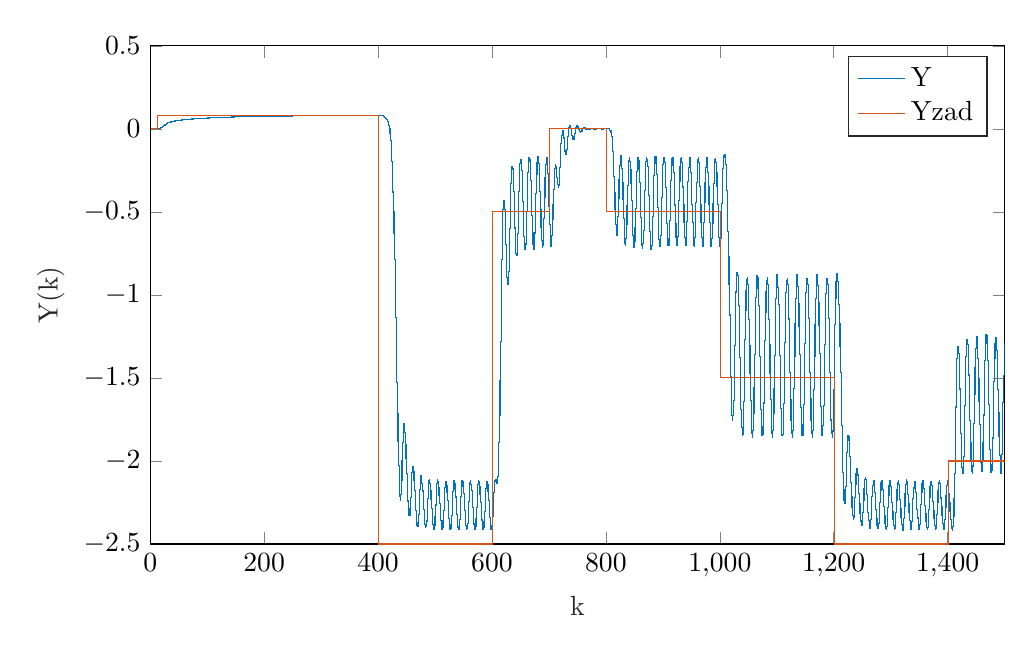
\begin{tikzpicture}

\begin{axis}[%
width=4.272in,
height=2.491in,
at={(0.717in,0.423in)},
scale only axis,
xmin=0,
xmax=1500,
xlabel style={font=\color{white!15!black}},
xlabel={k},
ymin=-2.5,
ymax=0.5,
ylabel style={font=\color{white!15!black}},
ylabel={Y(k)},
axis background/.style={fill=white},
legend style={legend cell align=left, align=left, draw=white!15!black}
]
\addplot[const plot, color=mycolor1] table[row sep=crcr] {%
1	0\\
2	0\\
3	0\\
4	0\\
5	0\\
6	0\\
7	0\\
8	0\\
9	0\\
10	0\\
11	0\\
12	0\\
13	0\\
14	0\\
15	0\\
16	0\\
17	0.00334251881758044\\
18	0.00663869844795659\\
19	0.00713745921451116\\
20	0.00797344068450235\\
21	0.0101107482717386\\
22	0.0129211846739813\\
23	0.0157474369308877\\
24	0.0189262514837671\\
25	0.0224773555655986\\
26	0.025810304078217\\
27	0.0286030623879287\\
28	0.0309009411921089\\
29	0.0328319573758937\\
30	0.0344349806658181\\
31	0.0357757657176456\\
32	0.0369820257737093\\
33	0.0381432072642584\\
34	0.0392797695256926\\
35	0.0403813085884319\\
36	0.0414400668700454\\
37	0.0424478311591768\\
38	0.0433923574419183\\
39	0.0442670869040099\\
40	0.0450756362818778\\
41	0.0458271544812484\\
42	0.0465306714067775\\
43	0.0471938752185645\\
44	0.0478234279141678\\
45	0.0484243570991366\\
46	0.0489997335210229\\
47	0.0495513198851957\\
48	0.0500804575105639\\
49	0.0505884472350941\\
50	0.0510765865273898\\
51	0.0515462062232189\\
52	0.0519986930878566\\
53	0.0524354264754257\\
54	0.0528576833017016\\
55	0.0532665950035421\\
56	0.0536631545859174\\
57	0.0540482335773781\\
58	0.0544225979785377\\
59	0.0547869280243986\\
60	0.0551418388301388\\
61	0.0554878942885314\\
62	0.0558256135932966\\
63	0.0561554747932677\\
64	0.0564779177522373\\
65	0.0567933465898736\\
66	0.0571021317753448\\
67	0.0574046125151812\\
68	0.0577010995677652\\
69	0.0579918780836872\\
70	0.058277210184349\\
71	0.0585573372549776\\
72	0.0588324819813362\\
73	0.059102850121145\\
74	0.059368632028941\\
75	0.0596300039968032\\
76	0.0598871294644611\\
77	0.0601401601221757\\
78	0.0603892369169668\\
79	0.0606344909729682\\
80	0.0608760444341496\\
81	0.0611140112332708\\
82	0.0613484977906274\\
83	0.0615796036481812\\
84	0.0618074220454539\\
85	0.0620320404429482\\
86	0.062253540998292\\
87	0.0624720009999684\\
88	0.0626874932629613\\
89	0.0629000864899715\\
90	0.0631098456013376\\
91	0.0633168320364725\\
92	0.063521104029358\\
93	0.0637227168603936\\
94	0.0639217230866827\\
95	0.0641181727526698\\
96	0.0643121135828754\\
97	0.064503591158315\\
98	0.0646926490780418\\
99	0.0648793291071171\\
100	0.0650636713121912\\
101	0.0652457141857709\\
102	0.0654254947601475\\
103	0.0656030487118752\\
104	0.0657784104576066\\
105	0.0659516132420253\\
106	0.0661226892185475\\
107	0.0662916695234057\\
108	0.0664585843436762\\
109	0.0666234629797611\\
110	0.0667863339027924\\
111	0.066947224807384\\
112	0.0671061626601236\\
113	0.0672631737441593\\
114	0.0674182837002071\\
115	0.0675715175642797\\
116	0.0677228998024066\\
117	0.0678724543425981\\
118	0.0680202046042798\\
119	0.0681661735254097\\
120	0.0683103835874666\\
121	0.0684528568384893\\
122	0.0685936149143243\\
123	0.068732679058232\\
124	0.0688700701389864\\
125	0.0690058086675912\\
126	0.0691399148127275\\
127	0.0692724084150369\\
128	0.0694033090003357\\
129	0.069532635791848\\
130	0.0696604077215383\\
131	0.0697866434406175\\
132	0.0699113613292902\\
133	0.070034579505805\\
134	0.0701563158348661\\
135	0.0702765879354566\\
136	0.0703954131881235\\
137	0.0705128087417678\\
138	0.0706287915199798\\
139	0.070743378226957\\
140	0.0708565853530391\\
141	0.070968429179891\\
142	0.0710789257853625\\
143	0.0711880910480512\\
144	0.0712959406515928\\
145	0.071402490088701\\
146	0.0715077546649773\\
147	0.0716117495025092\\
148	0.0717144895432743\\
149	0.0718159895523662\\
150	0.0719162641210557\\
151	0.0720153276697016\\
152	0.0721131944505229\\
153	0.0722098785502426\\
154	0.0723053938926155\\
155	0.0723997542408464\\
156	0.0724929731999103\\
157	0.0725850642187798\\
158	0.0726760405925694\\
159	0.0727659154646006\\
160	0.0728547018283965\\
161	0.0729424125296096\\
162	0.0730290602678883\\
163	0.0731146575986877\\
164	0.0731992169350271\\
165	0.0732827505492001\\
166	0.0733652705744393\\
167	0.0734467890065398\\
168	0.0735273177054439\\
169	0.0736068683967899\\
170	0.0736854526734279\\
171	0.0737630819969042\\
172	0.0738397676989163\\
173	0.0739155209827417\\
174	0.0739903529246405\\
175	0.0740642744752342\\
176	0.0741372964608624\\
177	0.0742094295849182\\
178	0.0742806844291639\\
179	0.0743510714550274\\
180	0.0744206010048812\\
181	0.0744892833033044\\
182	0.074557128458328\\
183	0.074624146462666\\
184	0.0746903471949303\\
185	0.074755740420833\\
186	0.0748203357943739\\
187	0.0748841428590159\\
188	0.074947171048847\\
189	0.0750094296897312\\
190	0.0750709280004466\\
191	0.0751316750938125\\
192	0.0751916799778057\\
193	0.0752509515566656\\
194	0.0753094986319885\\
195	0.0753673299038124\\
196	0.0754244539716905\\
197	0.0754808793357559\\
198	0.075536614397776\\
199	0.0755916674621971\\
200	0.0756460467371802\\
201	0.0756997603356264\\
202	0.0757528162761948\\
203	0.0758052224843092\\
204	0.0758569867931577\\
205	0.0759081169446821\\
206	0.0759586205905593\\
207	0.0760085052931737\\
208	0.0760577785265803\\
209	0.0761064476774607\\
210	0.0761545200460688\\
211	0.0762020028471695\\
212	0.0762489032109682\\
213	0.076295228184032\\
214	0.0763409847302027\\
215	0.0763861797315019\\
216	0.0764308199890271\\
217	0.0764749122238404\\
218	0.0765184630778484\\
219	0.0765614791146747\\
220	0.0766039668205238\\
221	0.0766459326050371\\
222	0.0766873828021414\\
223	0.0767283236708888\\
224	0.0767687613962891\\
225	0.0768087020901344\\
226	0.0768481517918159\\
227	0.0768871164691322\\
228	0.0769256020190915\\
229	0.0769636142687043\\
230	0.0770011589757697\\
231	0.0770382418296536\\
232	0.0770748684520592\\
233	0.0771110443977907\\
234	0.0771467751555086\\
235	0.0771820661484782\\
236	0.0772169227353104\\
237	0.0772513502106953\\
238	0.0772853538061287\\
239	0.0773189386906307\\
240	0.0773521099714576\\
241	0.0773848726948069\\
242	0.0774172318465143\\
243	0.0774491923527442\\
244	0.0774807590806735\\
245	0.0775119368391675\\
246	0.0775427303794498\\
247	0.0775731443957643\\
248	0.0776031835260317\\
249	0.0776328523524979\\
250	0.0776621554023763\\
251	0.0776910971484835\\
252	0.077719682009868\\
253	0.0777479143524324\\
254	0.0777757984895493\\
255	0.0778033386826706\\
256	0.0778305391419299\\
257	0.0778574040267394\\
258	0.0778839374463792\\
259	0.0779101434605821\\
260	0.07793602608011\\
261	0.077961589267326\\
262	0.0779868369367591\\
263	0.0780117729556636\\
264	0.078036401144572\\
265	0.0780607252778417\\
266	0.0780847490841968\\
267	0.0781084762472628\\
268	0.0781319104060963\\
269	0.078155055155708\\
270	0.0781779140475814\\
271	0.0782004905901845\\
272	0.0782227882494763\\
273	0.078244810449408\\
274	0.0782665605724183\\
275	0.0782880419599232\\
276	0.0783092579128011\\
277	0.0783302116918713\\
278	0.078350906518368\\
279	0.0783713455744092\\
280	0.0783915320034594\\
281	0.0784114689107882\\
282	0.0784311593639232\\
283	0.0784506063930977\\
284	0.078469812991694\\
285	0.0784887821166806\\
286	0.0785075166890461\\
287	0.0785260195942263\\
288	0.0785442936825283\\
289	0.0785623417695482\\
290	0.0785801666365854\\
291	0.0785977710310512\\
292	0.0786151576668733\\
293	0.0786323292248955\\
294	0.078649288353273\\
295	0.0786660376678631\\
296	0.0786825797526109\\
297	0.0786989171599321\\
298	0.0787150524110892\\
299	0.0787309879965657\\
300	0.0787467263764341\\
301	0.078762269980721\\
302	0.078777621209767\\
303	0.0787927824345834\\
304	0.0788077559972038\\
305	0.0788225442110326\\
306	0.0788371493611886\\
307	0.0788515737048454\\
308	0.0788658194715672\\
309	0.0788798888636412\\
310	0.0788937840564057\\
311	0.078907507198575\\
312	0.0789210604125596\\
313	0.0789344457947838\\
314	0.0789476654159984\\
315	0.078960721321591\\
316	0.0789736155318917\\
317	0.0789863500424753\\
318	0.078998926824461\\
319	0.0790113478248069\\
320	0.0790236149666027\\
321	0.0790357301493581\\
322	0.0790476952492876\\
323	0.0790595121195926\\
324	0.0790711825907401\\
325	0.0790827084707374\\
326	0.0790940915454046\\
327	0.079105333578643\\
328	0.079116436312701\\
329	0.0791274014684363\\
330	0.0791382307455757\\
331	0.0791489258229709\\
332	0.0791594883588522\\
333	0.0791699199910785\\
334	0.079180222337385\\
335	0.0791903969956272\\
336	0.0792004455440226\\
337	0.0792103695413892\\
338	0.0792201705273816\\
339	0.0792298500227239\\
340	0.0792394095294394\\
341	0.0792488505310791\\
342	0.0792581744929457\\
343	0.0792673828623159\\
344	0.0792764770686601\\
345	0.079285458523859\\
346	0.079294328622418\\
347	0.079303088741679\\
348	0.0793117402420293\\
349	0.0793202844671085\\
350	0.0793287227440127\\
351	0.0793370563834964\\
352	0.0793452866801716\\
353	0.0793534149127047\\
354	0.0793614423440118\\
355	0.0793693702214501\\
356	0.0793771997770086\\
357	0.0793849322274951\\
358	0.0793925687747225\\
359	0.0794001106056915\\
360	0.0794075588927713\\
361	0.0794149147938795\\
362	0.0794221794526576\\
363	0.0794293539986467\\
364	0.079436439547459\\
365	0.0794434372009487\\
366	0.0794503480473806\\
367	0.0794571731615957\\
368	0.0794639136051763\\
369	0.0794705704266077\\
370	0.0794771446614389\\
371	0.0794836373324413\\
372	0.0794900494497646\\
373	0.079496382011092\\
374	0.0795026360017927\\
375	0.0795088123950729\\
376	0.0795149121521249\\
377	0.0795209362222745\\
378	0.0795268855431265\\
379	0.0795327610407081\\
380	0.0795385636296117\\
381	0.0795442942131343\\
382	0.0795499536834169\\
383	0.079555542921581\\
384	0.0795610627978637\\
385	0.0795665141717519\\
386	0.0795718978921138\\
387	0.0795772147973296\\
388	0.0795824657154202\\
389	0.0795876514641743\\
390	0.0795927728512745\\
391	0.0795978306744211\\
392	0.0796028257214552\\
393	0.0796077587704796\\
394	0.0796126305899782\\
395	0.0796174419389351\\
396	0.0796221935669508\\
397	0.0796268862143576\\
398	0.0796315206123338\\
399	0.0796360974830165\\
400	0.0796406175396123\\
401	0.0796450814865077\\
402	0.0796494900193771\\
403	0.0796538438252908\\
404	0.0796581435828201\\
405	0.0796623899621425\\
406	0.0791124339710531\\
407	0.0782854608837616\\
408	0.0781940655394372\\
409	0.0767400355760779\\
410	0.0742629885211295\\
411	0.0712487098074998\\
412	0.0679973503748701\\
413	0.0646263420719462\\
414	0.0610834472628353\\
415	0.0571174039274092\\
416	0.0522106601899206\\
417	0.0454970374771302\\
418	0.0357002742900133\\
419	0.0211336870933039\\
420	-0.000213679614859927\\
421	-0.03051195775733\\
422	-0.0718873985697449\\
423	-0.12623609547906\\
424	-0.195097575517954\\
425	-0.279604954579873\\
426	-0.380502788569483\\
427	-0.498208743244067\\
428	-0.632892097412388\\
429	-0.784547107726996\\
430	-0.953047564836426\\
431	-1.13817691013313\\
432	-1.33398032235303\\
433	-1.5288883223013\\
434	-1.71323701606773\\
435	-1.88124979283007\\
436	-2.0284765120883\\
437	-2.14388615175127\\
438	-2.2153375757695\\
439	-2.23510834170274\\
440	-2.20043475405845\\
441	-2.11487953708438\\
442	-1.99889439921092\\
443	-1.88896658709549\\
444	-1.80936760970016\\
445	-1.77186868316992\\
446	-1.78064702845168\\
447	-1.82856692515604\\
448	-1.90149904091715\\
449	-1.98704865236221\\
450	-2.07646807378393\\
451	-2.1638412091569\\
452	-2.24112153350905\\
453	-2.29864754770553\\
454	-2.3285579084651\\
455	-2.32580668323831\\
456	-2.2881254008832\\
457	-2.22054802264854\\
458	-2.13971990187326\\
459	-2.07130820342056\\
460	-2.03325402802656\\
461	-2.03444865693171\\
462	-2.06620947502714\\
463	-2.11641809111954\\
464	-2.17611608970437\\
465	-2.23896205804578\\
466	-2.30048913141319\\
467	-2.35214536234355\\
468	-2.38530208903838\\
469	-2.39372768003229\\
470	-2.37367154113613\\
471	-2.32388970531019\\
472	-2.25155903540669\\
473	-2.17444785086794\\
474	-2.11565697724238\\
475	-2.09022399200839\\
476	-2.09931775026227\\
477	-2.13301542888924\\
478	-2.18107145163415\\
479	-2.23605387342364\\
480	-2.29275023894913\\
481	-2.34487483338981\\
482	-2.38397929807152\\
483	-2.40274106110179\\
484	-2.39619131929437\\
485	-2.36167525154869\\
486	-2.3016423246376\\
487	-2.22791259724594\\
488	-2.16087864776218\\
489	-2.11945852733372\\
490	-2.11444461365439\\
491	-2.13814649836482\\
492	-2.17940603661405\\
493	-2.23003105015663\\
494	-2.28418733036052\\
495	-2.33745250423592\\
496	-2.38150976850465\\
497	-2.40815945887221\\
498	-2.41152748592884\\
499	-2.38808381081474\\
500	-2.33694154177586\\
501	-2.26545493001172\\
502	-2.19093516923124\\
503	-2.1356171168751\\
504	-2.11394090988524\\
505	-2.1249598166731\\
506	-2.15860372125417\\
507	-2.2053151668796\\
508	-2.2581780630764\\
509	-2.31235680761595\\
510	-2.36109202970844\\
511	-2.39602024664455\\
512	-2.41021610933091\\
513	-2.39908611660335\\
514	-2.3602970798426\\
515	-2.29734253637976\\
516	-2.22325414534657\\
517	-2.15901899669094\\
518	-2.1224340711743\\
519	-2.12118767514641\\
520	-2.14700719695073\\
521	-2.18919753549493\\
522	-2.23992992246569\\
523	-2.29364983515994\\
524	-2.34533973512797\\
525	-2.38668517692632\\
526	-2.40983414692151\\
527	-2.40925458964136\\
528	-2.38172951344513\\
529	-2.32749748221423\\
530	-2.25539132808025\\
531	-2.18368150399779\\
532	-2.13337943122023\\
533	-2.11770722930599\\
534	-2.13316433838881\\
535	-2.16928949681935\\
536	-2.21707603226925\\
537	-2.27003984091234\\
538	-2.32367754707021\\
539	-2.37064598848578\\
540	-2.40259073612179\\
541	-2.41294862942836\\
542	-2.39749842883473\\
543	-2.35425573461417\\
544	-2.28792334416439\\
545	-2.21302308173705\\
546	-2.15144144290487\\
547	-2.11983391369019\\
548	-2.12272221725996\\
549	-2.15116592557723\\
550	-2.19485879204784\\
551	-2.24628362791947\\
552	-2.30013103360763\\
553	-2.35076796573651\\
554	-2.38986350392134\\
555	-2.40989172180212\\
556	-2.40564669977532\\
557	-2.37421612714749\\
558	-2.31696778876524\\
559	-2.24421105938386\\
560	-2.17518449350475\\
561	-2.12974347236689\\
562	-2.11992478262948\\
563	-2.13977262044338\\
564	-2.17842968505303\\
565	-2.22740351221315\\
566	-2.28061492635946\\
567	-2.33387332619865\\
568	-2.3792618933617\\
569	-2.40843095981841\\
570	-2.41516352966656\\
571	-2.39559656439718\\
572	-2.34808330506846\\
573	-2.27850755212634\\
574	-2.20282261600019\\
575	-2.14376578542023\\
576	-2.1169246709986\\
577	-2.1237985218867\\
578	-2.15479237024595\\
579	-2.19996660147384\\
580	-2.25209837408589\\
581	-2.30611032308301\\
582	-2.35576849087632\\
583	-2.3927259104161\\
584	-2.40977100572508\\
585	-2.40201268930468\\
586	-2.36683321205966\\
587	-2.30669986136816\\
588	-2.23333339829285\\
589	-2.16687614276033\\
590	-2.12609941963097\\
591	-2.12132046188964\\
592	-2.14482407234271\\
593	-2.18561229465594\\
594	-2.23561163273797\\
595	-2.28907335549485\\
596	-2.34147946335101\\
597	-2.38453569121112\\
598	-2.41013166700018\\
599	-2.41247489315258\\
600	-2.3881029474345\\
601	-2.33634329561981\\
602	-2.26480874029533\\
603	-2.19093840292973\\
604	-2.13670019341794\\
605	-2.11628847678084\\
606	-2.1101537938682\\
607	-2.12249384877554\\
608	-2.13719536118062\\
609	-2.13274541784778\\
610	-2.09495299584431\\
611	-2.01558617669406\\
612	-1.89135450545129\\
613	-1.72323340985572\\
614	-1.51615009140887\\
615	-1.27900570468661\\
616	-1.02482688073894\\
617	-0.787021863324449\\
618	-0.60270722377129\\
619	-0.484492253612885\\
620	-0.430602095883164\\
621	-0.433872300866812\\
622	-0.485898578001959\\
623	-0.578820720362755\\
624	-0.696269182360772\\
625	-0.80994387647798\\
626	-0.894922836275648\\
627	-0.935332920738251\\
628	-0.923221672064436\\
629	-0.858017655306721\\
630	-0.746416944157045\\
631	-0.6021448843648\\
632	-0.451670769319791\\
633	-0.331252332653745\\
634	-0.256183188851737\\
635	-0.227721141625848\\
636	-0.24174031055161\\
637	-0.292810064652861\\
638	-0.375789511505721\\
639	-0.482814162980429\\
640	-0.596811962682944\\
641	-0.692839746609454\\
642	-0.750891703305945\\
643	-0.759869023351789\\
644	-0.717027443795506\\
645	-0.627836293938198\\
646	-0.505559665745078\\
647	-0.375443322431684\\
648	-0.271168150433401\\
649	-0.207400301644859\\
650	-0.185688458497993\\
651	-0.202544482341827\\
652	-0.253304305758557\\
653	-0.333577043427058\\
654	-0.43715433615405\\
655	-0.549442090055115\\
656	-0.647798124472618\\
657	-0.711563490902635\\
658	-0.728140824057937\\
659	-0.693523028265826\\
660	-0.612130770804776\\
661	-0.496419015359293\\
662	-0.369436570107556\\
663	-0.264917697932507\\
664	-0.199034289952907\\
665	-0.174306945436386\\
666	-0.187652685748362\\
667	-0.234602804989254\\
668	-0.31088263728747\\
669	-0.411708169315584\\
670	-0.524157099697409\\
671	-0.627020109462872\\
672	-0.698736972022171\\
673	-0.725009088389933\\
674	-0.700218827454066\\
675	-0.627219673729258\\
676	-0.517058777357029\\
677	-0.388290558441507\\
678	-0.276098357966115\\
679	-0.200693488052712\\
680	-0.16664509573495\\
681	-0.171413414770466\\
682	-0.210549391366334\\
683	-0.279653059893158\\
684	-0.374991752463468\\
685	-0.485900102929445\\
686	-0.593335518133237\\
687	-0.67461929533245\\
688	-0.713191749527659\\
689	-0.701342927241307\\
690	-0.639919884131\\
691	-0.538138909148964\\
692	-0.412480297984612\\
693	-0.296276047353161\\
694	-0.213850524259104\\
695	-0.172410477266082\\
696	-0.170366202311722\\
697	-0.203511838614862\\
698	-0.267417500627735\\
699	-0.358231390106809\\
700	-0.466675111558253\\
701	-0.575239465491711\\
702	-0.66070208663395\\
703	-0.705255979498099\\
704	-0.700048672979493\\
705	-0.644836864411475\\
706	-0.547825270386168\\
707	-0.455215631798658\\
708	-0.367921339581302\\
709	-0.28979986706346\\
710	-0.23685598648257\\
711	-0.21712129320904\\
712	-0.225003560285683\\
713	-0.253086136545025\\
714	-0.295236448026811\\
715	-0.335891441459823\\
716	-0.35571201973348\\
717	-0.343615965057195\\
718	-0.2993933936189\\
719	-0.232262998458066\\
720	-0.157049543831817\\
721	-0.0893790516059391\\
722	-0.0404613478598009\\
723	-0.0139094916686101\\
724	-0.0090824091904236\\
725	-0.02378858283997\\
726	-0.0552484540581584\\
727	-0.0958597869720725\\
728	-0.133487367657603\\
729	-0.155342306230144\\
730	-0.152740881785768\\
731	-0.126932811056434\\
732	-0.0873862092754728\\
733	-0.0458715119092312\\
734	-0.0120325818447793\\
735	0.0100930742967469\\
736	0.0197234697523889\\
737	0.0169611272058478\\
738	0.00324362694482052\\
739	-0.0175438314570938\\
740	-0.0395876226696478\\
741	-0.0570524557093219\\
742	-0.065096248510784\\
743	-0.0611796266278013\\
744	-0.046841441293946\\
745	-0.0272969649509784\\
746	-0.00828795538477268\\
747	0.00642174570612104\\
748	0.0152011035185386\\
749	0.0176288204571165\\
750	0.0141676828403557\\
751	0.00640638890915333\\
752	-0.0032040317020049\\
753	-0.0121024386888433\\
754	-0.0181920930258086\\
755	-0.0201953900830726\\
756	-0.0180020689153278\\
757	-0.0126999262417414\\
758	-0.00604427152557883\\
759	0.000246089787810733\\
760	0.00491774757722922\\
761	0.00729875804719891\\
762	0.00728393061312094\\
763	0.00527664349151318\\
764	0.00205235532495998\\
765	-0.00145503462491535\\
766	-0.0043772501647396\\
767	-0.0060953115634349\\
768	-0.00635890799004894\\
769	-0.00530848559087528\\
770	-0.00338334087043199\\
771	-0.00115684263183436\\
772	0.000828943743008441\\
773	0.00218033925501936\\
774	0.00270952404027397\\
775	0.00243917875459399\\
776	0.00156424206324023\\
777	0.000383742236784428\\
778	-0.000780041147819997\\
779	-0.00165701241382844\\
780	-0.00208385473929013\\
781	-0.0020270181867996\\
782	-0.00157115540414824\\
783	-0.000880187652238522\\
784	-0.000145625371183369\\
785	0.000462319158884336\\
786	0.000829737496312031\\
787	0.000915148187658454\\
788	0.000746926267547609\\
789	0.000405881479882813\\
790	-9.5976636282122e-07\\
791	-0.000368467535420943\\
792	-0.000616994859119766\\
793	-0.000706711992271641\\
794	-0.000640601763957121\\
795	-0.000457016053045507\\
796	-0.0002151654418196\\
797	2.18558874964994e-05\\
798	0.000202112032932071\\
799	0.000294812891374185\\
800	0.000293869904928376\\
801	0.000215319374549913\\
802	9.01905543470429e-05\\
803	-4.48784634772934e-05\\
804	-0.000156835364716866\\
805	-0.000223173308633144\\
806	-0.00420003741676484\\
807	-0.00759300864922998\\
808	-0.0114767580847866\\
809	-0.0232066343392653\\
810	-0.0464943285594827\\
811	-0.0835161908940249\\
812	-0.135719305606911\\
813	-0.204099744074412\\
814	-0.289110211366898\\
815	-0.386457764365434\\
816	-0.486192001145528\\
817	-0.573478732658661\\
818	-0.629496798431777\\
819	-0.641286931761105\\
820	-0.604992299181025\\
821	-0.525691580757904\\
822	-0.416664439806119\\
823	-0.30423483771963\\
824	-0.218174058933997\\
825	-0.170034608674684\\
826	-0.160207409197677\\
827	-0.185320720773194\\
828	-0.241292088054053\\
829	-0.324408988405908\\
830	-0.428037276386122\\
831	-0.537666746651335\\
832	-0.63169349112061\\
833	-0.690288443944572\\
834	-0.701573100233941\\
835	-0.662379736801093\\
836	-0.578104698191224\\
837	-0.46214815665979\\
838	-0.340522367506644\\
839	-0.245136058921181\\
840	-0.189084103256707\\
841	-0.173305108273871\\
842	-0.19434332215672\\
843	-0.247805099712147\\
844	-0.329623300052152\\
845	-0.433332410242328\\
846	-0.544320554246108\\
847	-0.640403398124272\\
848	-0.701359940146139\\
849	-0.715002056259316\\
850	-0.67778795312133\\
851	-0.59467098538745\\
852	-0.47862368040509\\
853	-0.354361600739232\\
854	-0.254667879530666\\
855	-0.194017198883642\\
856	-0.174067254170252\\
857	-0.191532142251252\\
858	-0.241982521267951\\
859	-0.321253697878365\\
860	-0.423650856122211\\
861	-0.53533526947662\\
862	-0.634567394582287\\
863	-0.700495595467331\\
864	-0.719948327597227\\
865	-0.688412881540201\\
866	-0.609862692256994\\
867	-0.496384612011142\\
868	-0.369993116519993\\
869	-0.264590008031061\\
870	-0.197154305121824\\
871	-0.170669567352516\\
872	-0.182211943344422\\
873	-0.227363541212805\\
874	-0.301865556653595\\
875	-0.401534440564338\\
876	-0.514122913105903\\
877	-0.618948332836974\\
878	-0.694068996178037\\
879	-0.724482689557164\\
880	-0.70390356904205\\
881	-0.634526139314372\\
882	-0.526787964085748\\
883	-0.398043793045614\\
884	-0.283395140340355\\
885	-0.204672336115517\\
886	-0.167358678959801\\
887	-0.169193968653405\\
888	-0.205764745492927\\
889	-0.272625347381031\\
890	-0.36597935499684\\
891	-0.475756607164257\\
892	-0.583614419947836\\
893	-0.666648423434228\\
894	-0.70775804174884\\
895	-0.698747066257286\\
896	-0.640011313817984\\
897	-0.540361191985377\\
898	-0.415976629024277\\
899	-0.299533027541325\\
900	-0.216136471495339\\
901	-0.173535722146743\\
902	-0.17035729137907\\
903	-0.202468770328566\\
904	-0.265454149110993\\
905	-0.355452573316428\\
906	-0.463447458712345\\
907	-0.572210891434038\\
908	-0.658426101369601\\
909	-0.704061820542776\\
910	-0.700059430158789\\
911	-0.64597719063376\\
912	-0.549832901562487\\
913	-0.427192934890955\\
914	-0.309392194999651\\
915	-0.223305551562782\\
916	-0.177844308336754\\
917	-0.172071862811916\\
918	-0.201974841757981\\
919	-0.263126941222217\\
920	-0.351611835347346\\
921	-0.458869541574931\\
922	-0.568123865618089\\
923	-0.655856373041275\\
924	-0.703614948749017\\
925	-0.701946263818735\\
926	-0.650017263959876\\
927	-0.555465443233899\\
928	-0.433552929544621\\
929	-0.314917913032949\\
930	-0.22736093611146\\
931	-0.18038561160704\\
932	-0.173272913515725\\
933	-0.202062955023128\\
934	-0.262316770533151\\
935	-0.350083132337333\\
936	-0.457012548837212\\
937	-0.566527450464148\\
938	-0.655152341478067\\
939	-0.704232920930513\\
940	-0.704050437736011\\
941	-0.653503510791085\\
942	-0.559962747067824\\
943	-0.438470402240092\\
944	-0.319159380814694\\
945	-0.230497934513011\\
946	-0.1824109024764\\
947	-0.174331651987999\\
948	-0.202334703219179\\
949	-0.261968116198494\\
950	-0.349252148334348\\
951	-0.455974769535383\\
952	-0.565682146627719\\
953	-0.654944458157057\\
954	-0.704971452066545\\
955	-0.705854116220358\\
956	-0.656297016392407\\
957	-0.563475550440936\\
958	-0.442268778170366\\
959	-0.322426705607621\\
960	-0.232921279705597\\
961	-0.183992386597093\\
962	-0.175186601720077\\
963	-0.202603005952727\\
964	-0.261778688773838\\
965	-0.3487114126871\\
966	-0.455287956758383\\
967	-0.565141371448268\\
968	-0.654869589234877\\
969	-0.705583597168855\\
970	-0.70723784582875\\
971	-0.658397166992718\\
972	-0.566095622365097\\
973	-0.445093104028938\\
974	-0.324854395806096\\
975	-0.234723972892069\\
976	-0.185173584800002\\
977	-0.175832917051703\\
978	-0.202818813608868\\
979	-0.261659955004519\\
980	-0.348337242039997\\
981	-0.454808917018021\\
982	-0.564770233402832\\
983	-0.654837633330778\\
984	-0.706050486300736\\
985	-0.708264714658848\\
986	-0.659944179437262\\
987	-0.568020508590564\\
988	-0.447166731106666\\
989	-0.32663668744807\\
990	-0.236048296811732\\
991	-0.186043004810237\\
992	-0.176311271105641\\
993	-0.202982857754538\\
994	-0.261580201241897\\
995	-0.348071779271229\\
996	-0.454467668771855\\
997	-0.564508014377075\\
998	-0.65482212902323\\
999	-0.706397427455215\\
1000	-0.709018514124029\\
1001	-0.661076119972655\\
1002	-0.569427546483384\\
1003	-0.448682542141318\\
1004	-0.327939651419277\\
1005	-0.237016868318739\\
1006	-0.186679565163467\\
1007	-0.159940080796782\\
1008	-0.153939373817896\\
1009	-0.172468184299044\\
1010	-0.21593130845267\\
1011	-0.28341934243632\\
1012	-0.373609380442853\\
1013	-0.485146527774542\\
1014	-0.616797183943521\\
1015	-0.767498507801389\\
1016	-0.936356035426203\\
1017	-1.12127026195767\\
1018	-1.31225778010792\\
1019	-1.4898888592009\\
1020	-1.63273240482258\\
1021	-1.72518586002909\\
1022	-1.75832309197624\\
1023	-1.72869784684663\\
1024	-1.63751367561671\\
1025	-1.49017813246446\\
1026	-1.3026432253681\\
1027	-1.12246365904555\\
1028	-0.982243445337012\\
1029	-0.895312386030091\\
1030	-0.863906176589529\\
1031	-0.884924911448334\\
1032	-0.953088024164304\\
1033	-1.06259728566135\\
1034	-1.2079486312864\\
1035	-1.37558654608117\\
1036	-1.5449560102318\\
1037	-1.69182359272325\\
1038	-1.79694488496465\\
1039	-1.8483527205701\\
1040	-1.83998817867423\\
1041	-1.77068777144523\\
1042	-1.6435254091078\\
1043	-1.4655314219071\\
1044	-1.26776423599883\\
1045	-1.09560140075013\\
1046	-0.972611159307915\\
1047	-0.906188402023585\\
1048	-0.895548917052605\\
1049	-0.93618268336132\\
1050	-1.02226596559261\\
1051	-1.14790128454775\\
1052	-1.30362572002819\\
1053	-1.47388877935268\\
1054	-1.63340857559199\\
1055	-1.75924095363091\\
1056	-1.83622190216785\\
1057	-1.85568312005334\\
1058	-1.81427621708437\\
1059	-1.71314638189659\\
1060	-1.55747218741799\\
1061	-1.3605801644602\\
1062	-1.16925865394514\\
1063	-1.01792299881839\\
1064	-0.921045777551096\\
1065	-0.881271847117812\\
1066	-0.89553138241154\\
1067	-0.958394552649852\\
1068	-1.06384455676587\\
1069	-1.20614781319376\\
1070	-1.37177867341744\\
1071	-1.54056916864071\\
1072	-1.68812609571117\\
1073	-1.79480902300941\\
1074	-1.84832891683749\\
1075	-1.84236171846211\\
1076	-1.77551929733388\\
1077	-1.65067441991978\\
1078	-1.47466203707665\\
1079	-1.27690340163491\\
1080	-1.10354774907986\\
1081	-0.978868681940057\\
1082	-0.910646790820584\\
1083	-0.898295333484768\\
1084	-0.937393184740862\\
1085	-1.02214486176042\\
1086	-1.14664914381621\\
1087	-1.30161167599054\\
1088	-1.47147976931097\\
1089	-1.631138779797\\
1090	-1.7575931062362\\
1091	-1.83551252085757\\
1092	-1.85609303286874\\
1093	-1.815873310596\\
1094	-1.71590060463558\\
1095	-1.56126229434894\\
1096	-1.36447238729946\\
1097	-1.17206136665866\\
1098	-1.01908763904032\\
1099	-0.920458753817744\\
1100	-0.879020468613131\\
1101	-0.89178106455981\\
1102	-0.953327062185603\\
1103	-1.05762950713632\\
1104	-1.19893205108587\\
1105	-1.36409432227723\\
1106	-1.53340338457686\\
1107	-1.68234875159887\\
1108	-1.79098412266145\\
1109	-1.84677439036086\\
1110	-1.84319508500602\\
1111	-1.77869027932692\\
1112	-1.65598399108308\\
1113	-1.48176732289965\\
1114	-1.28409614430706\\
1115	-1.10978955356311\\
1116	-0.983724519503016\\
1117	-0.91401127389501\\
1118	-0.900232119434811\\
1119	-0.938042602458859\\
1120	-1.02167241265299\\
1121	-1.14521835163558\\
1122	-1.29954659533783\\
1123	-1.46910575185172\\
1124	-1.62893204481233\\
1125	-1.75598398173979\\
1126	-1.8347815607355\\
1127	-1.85639866976943\\
1128	-1.81727247553974\\
1129	-1.7183623592642\\
1130	-1.5646740100909\\
1131	-1.36798226776102\\
1132	-1.17457897917766\\
1133	-1.02011426965673\\
1134	-0.919893179194022\\
1135	-0.876944191378676\\
1136	-0.888346014094462\\
1137	-0.94869934344227\\
1138	-1.05196358259528\\
1139	-1.19236123891952\\
1140	-1.35710119875225\\
1141	-1.52688106492735\\
1142	-1.67708487735159\\
1143	-1.78748964044591\\
1144	-1.84533774492553\\
1145	-1.84392362428883\\
1146	-1.78153989510451\\
1147	-1.6607765460716\\
1148	-1.48819528124787\\
1149	-1.29060705324036\\
1150	-1.11544118129878\\
1151	-0.988122579838621\\
1152	-0.917060595037731\\
1153	-0.901990756325852\\
1154	-0.93863799109267\\
1155	-1.02125466738944\\
1156	-1.14393566992792\\
1157	-1.29769125841355\\
1158	-1.46697103250562\\
1159	-1.62694647142673\\
1160	-1.75453498730372\\
1161	-1.83412187192204\\
1162	-1.85667120609269\\
1163	-1.81852892861285\\
1164	-1.72057550284581\\
1165	-1.56774331826984\\
1166	-1.37114072349829\\
1167	-1.17684006326384\\
1168	-1.02102965470539\\
1169	-0.919373949001207\\
1170	-0.875065919193271\\
1171	-0.885247133208483\\
1172	-0.944530423984198\\
1173	-1.04686417168195\\
1174	-1.18645143095886\\
1175	-1.35081394948649\\
1176	-1.52101570456611\\
1177	-1.67234686167536\\
1178	-1.78433684072561\\
1179	-1.84402901825062\\
1180	-1.84455593844258\\
1181	-1.78407495848638\\
1182	-1.66505655735276\\
1183	-1.49394723369542\\
1184	-1.29643626421685\\
1185	-1.12050233066226\\
1186	-0.992062302330599\\
1187	-0.919793877249799\\
1188	-0.903569922037658\\
1189	-0.939177457314905\\
1190	-1.02088906645666\\
1191	-1.14279781612103\\
1192	-1.2960419481912\\
1193	-1.4650718004691\\
1194	-1.62517888072672\\
1195	-1.75324416925918\\
1196	-1.83353307150211\\
1197	-1.85691196397145\\
1198	-1.81964564319883\\
1199	-1.72254442496306\\
1200	-1.57047559960769\\
1201	-1.37395302513953\\
1202	-1.17884976745589\\
1203	-1.0218379467373\\
1204	-0.918903408264326\\
1205	-0.873385627253361\\
1206	-0.882481724441049\\
1207	-0.918583157735694\\
1208	-0.97646955459219\\
1209	-1.06045564560044\\
1210	-1.17190439866275\\
1211	-1.31049794536961\\
1212	-1.46772957281151\\
1213	-1.63058016438689\\
1214	-1.78877014779202\\
1215	-1.93581861061713\\
1216	-2.0668079651595\\
1217	-2.17103881989108\\
1218	-2.23713582206363\\
1219	-2.25765459346322\\
1220	-2.22947354952683\\
1221	-2.15488316941731\\
1222	-2.05090323929205\\
1223	-1.95032266626303\\
1224	-1.87722208410031\\
1225	-1.8440374711108\\
1226	-1.85556070689763\\
1227	-1.9024964929671\\
1228	-1.97100213928806\\
1229	-2.05010164284602\\
1230	-2.13207824293612\\
1231	-2.21174052439945\\
1232	-2.28045560909417\\
1233	-2.32882744692592\\
1234	-2.34971762758083\\
1235	-2.33873003756773\\
1236	-2.294114220984\\
1237	-2.22242979732648\\
1238	-2.14180242747365\\
1239	-2.07713719128695\\
1240	-2.04484520726032\\
1241	-2.05041838150675\\
1242	-2.08431709524962\\
1243	-2.1349965622757\\
1244	-2.19405162617137\\
1245	-2.2555595166086\\
1246	-2.31415617710339\\
1247	-2.36123944244577\\
1248	-2.38872526209695\\
1249	-2.39093055467971\\
1250	-2.36458996392652\\
1251	-2.31015365114267\\
1252	-2.23705741977827\\
1253	-2.16448604292506\\
1254	-2.1136100379858\\
1255	-2.09757847354515\\
1256	-2.11355612990459\\
1257	-2.15102496118099\\
1258	-2.20062445923678\\
1259	-2.25561521481633\\
1260	-2.31131601750927\\
1261	-2.36053496716593\\
1262	-2.39484020961301\\
1263	-2.40748117621806\\
1264	-2.39407543925984\\
1265	-2.35251641941039\\
1266	-2.28714478384314\\
1267	-2.21213603222701\\
1268	-2.1493143816786\\
1269	-2.11576406044506\\
1270	-2.11726100947889\\
1271	-2.14507470211185\\
1272	-2.18866745411176\\
1273	-2.24034367718381\\
1274	-2.29465937063259\\
1275	-2.34623277156629\\
1276	-2.38672064031012\\
1277	-2.40843578223074\\
1278	-2.40601629129521\\
1279	-2.37641032868197\\
1280	-2.32049500671124\\
1281	-2.24796319012102\\
1282	-2.17768640341615\\
1283	-2.1300425346402\\
1284	-2.11759078148187\\
1285	-2.1355154586611\\
1286	-2.17313326939084\\
1287	-2.22169880428353\\
1288	-2.27493525795086\\
1289	-2.32850067031956\\
1290	-2.37474589872015\\
1291	-2.40531371130331\\
1292	-2.41381952640411\\
1293	-2.39622909882679\\
1294	-2.35073632061052\\
1295	-2.28267121492758\\
1296	-2.20732628849608\\
1297	-2.14705873126751\\
1298	-2.11795828644585\\
1299	-2.12295721225801\\
1300	-2.15276853767008\\
1301	-2.19727335894993\\
1302	-2.24910538189055\\
1303	-2.30307455470939\\
1304	-2.35323393259836\\
1305	-2.39124271810842\\
1306	-2.40973745675519\\
1307	-2.40367531534662\\
1308	-2.37029700543819\\
1309	-2.31154271855829\\
1310	-2.23846150587163\\
1311	-2.17077080480539\\
1312	-2.12775861190249\\
1313	-2.12087141849449\\
1314	-2.14292702510376\\
1315	-2.18286581360223\\
1316	-2.23245045086133\\
1317	-2.28580286450687\\
1318	-2.33884795351366\\
1319	-2.38337781618357\\
1320	-2.41106139780304\\
1321	-2.415867934914\\
1322	-2.39412391527273\\
1323	-2.34440183098189\\
1324	-2.27324327127162\\
1325	-2.19734662657756\\
1326	-2.13954099086164\\
1327	-2.11488090102976\\
1328	-2.12359069578625\\
1329	-2.15579527370011\\
1330	-2.20170959647507\\
1331	-2.25423594784325\\
1332	-2.30839643382089\\
1333	-2.35769677563437\\
1334	-2.39378028204456\\
1335	-2.40956855148512\\
1336	-2.40030601058207\\
1337	-2.36350336419017\\
1338	-2.30210802775857\\
1339	-2.22845395285968\\
1340	-2.16307697285578\\
1341	-2.12429081443322\\
1342	-2.12118692630379\\
1343	-2.14579230658372\\
1344	-2.1872511712742\\
1345	-2.23760501957434\\
1346	-2.29119646632315\\
1347	-2.34327517843985\\
1348	-2.38553696707591\\
1349	-2.40999167345894\\
1350	-2.41096836924289\\
1351	-2.38511946604993\\
1352	-2.33219750455833\\
1353	-2.26038776602616\\
1354	-2.18752306631096\\
1355	-2.1351220332732\\
1356	-2.11692328775028\\
1357	-2.13048038534221\\
1358	-2.16550091607036\\
1359	-2.21275926632479\\
1360	-2.26559871953055\\
1361	-2.31938240375051\\
1362	-2.36700978755991\\
1363	-2.40012550967561\\
1364	-2.412020008988\\
1365	-2.39832029239792\\
1366	-2.35689862849888\\
1367	-2.29195767529413\\
1368	-2.21740299140122\\
1369	-2.15474638215712\\
1370	-2.12110655699801\\
1371	-2.12229637122717\\
1372	-2.14965162620539\\
1373	-2.1927104985673\\
1374	-2.24383084828857\\
1375	-2.29760473748462\\
1376	-2.34865162847818\\
1377	-2.3886479356931\\
1378	-2.40993534907703\\
1379	-2.40717532768041\\
1380	-2.37733141789491\\
1381	-2.32130946111859\\
1382	-2.24881748487114\\
1383	-2.17870154896237\\
1384	-2.13128380580511\\
1385	-2.11908249400159\\
1386	-2.13713997835071\\
1387	-2.17476146927589\\
1388	-2.22324609009623\\
1389	-2.27635047388259\\
1390	-2.32975713594349\\
1391	-2.37578394480647\\
1392	-2.40607935160761\\
1393	-2.41428535084662\\
1394	-2.3963928810416\\
1395	-2.35061746187394\\
1396	-2.28236028986187\\
1397	-2.20699307118584\\
1398	-2.1469097518656\\
1399	-2.11812939310059\\
1400	-2.12337986802891\\
1401	-2.15333399408464\\
1402	-2.19790322328349\\
1403	-2.24974511552764\\
1404	-2.30368800255851\\
1405	-2.35374382885263\\
1406	-2.38326393275988\\
1407	-2.40766762154325\\
1408	-2.41759950112357\\
1409	-2.39689748767964\\
1410	-2.33558430971727\\
1411	-2.22871469038087\\
1412	-2.07551628564214\\
1413	-1.87904033603237\\
1414	-1.67532346674124\\
1415	-1.50256670779231\\
1416	-1.38065752173527\\
1417	-1.3162396415635\\
1418	-1.30880819230368\\
1419	-1.35432598272921\\
1420	-1.4458714891977\\
1421	-1.56690382350805\\
1422	-1.70101712698348\\
1423	-1.83681805297878\\
1424	-1.95555296421148\\
1425	-2.03832221013311\\
1426	-2.07247862853139\\
1427	-2.05120508496576\\
1428	-1.9724622499832\\
1429	-1.8382526813864\\
1430	-1.66636060621387\\
1431	-1.50136605650255\\
1432	-1.37304829542729\\
1433	-1.2946771250151\\
1434	-1.26975253054792\\
1435	-1.2965957324658\\
1436	-1.37105899168024\\
1437	-1.48251330017612\\
1438	-1.61468427857481\\
1439	-1.75363347353394\\
1440	-1.88676654540328\\
1441	-1.99452958399963\\
1442	-2.06018897462993\\
1443	-2.07362040049976\\
1444	-2.03006239803183\\
1445	-1.92919017348619\\
1446	-1.77450961721748\\
1447	-1.59687776181903\\
1448	-1.43854856701966\\
1449	-1.32343377723943\\
1450	-1.26083133187698\\
1451	-1.25199642272739\\
1452	-1.29406607483783\\
1453	-1.38234331499252\\
1454	-1.50341248635083\\
1455	-1.64079890410199\\
1456	-1.78182089476941\\
1457	-1.91135004146679\\
1458	-2.01020645587079\\
1459	-2.06355205730207\\
1460	-2.06279890458464\\
1461	-2.00444978743377\\
1462	-1.88925557249595\\
1463	-1.72343211920932\\
1464	-1.54599577372884\\
1465	-1.39515379103317\\
1466	-1.29080367597403\\
1467	-1.23993745481663\\
1468	-1.24255607251971\\
1469	-1.29517639849799\\
1470	-1.3928518577997\\
1471	-1.5203253131095\\
1472	-1.66103251675275\\
1473	-1.80318978057707\\
1474	-1.92987629829209\\
1475	-2.02221590588786\\
1476	-2.06670885289092\\
1477	-2.05585391887542\\
1478	-1.98705105886418\\
1479	-1.86181956642252\\
1480	-1.69264895187725\\
1481	-1.52186112064156\\
1482	-1.38304573997418\\
1483	-1.29251635529051\\
1484	-1.25539499406734\\
1485	-1.27079640404183\\
1486	-1.33489805524143\\
1487	-1.44010830438181\\
1488	-1.57036773822837\\
1489	-1.71033522647659\\
1490	-1.8494860012465\\
1491	-1.9679057054863\\
1492	-2.04710849502758\\
1493	-2.0755622752684\\
1494	-2.04736049507964\\
1495	-1.96122033815733\\
1496	-1.81979668672391\\
1497	-1.64535463445391\\
1498	-1.48327581443513\\
1499	-1.36096701653658\\
1500	-1.28982335884019\\
};
\addlegendentry{Y}

\addplot[const plot, color=mycolor2] table[row sep=crcr] {%
1	0\\
2	0\\
3	0\\
4	0\\
5	0\\
6	0\\
7	0\\
8	0\\
9	0\\
10	0\\
11	0\\
12	0.08\\
13	0.08\\
14	0.08\\
15	0.08\\
16	0.08\\
17	0.08\\
18	0.08\\
19	0.08\\
20	0.08\\
21	0.08\\
22	0.08\\
23	0.08\\
24	0.08\\
25	0.08\\
26	0.08\\
27	0.08\\
28	0.08\\
29	0.08\\
30	0.08\\
31	0.08\\
32	0.08\\
33	0.08\\
34	0.08\\
35	0.08\\
36	0.08\\
37	0.08\\
38	0.08\\
39	0.08\\
40	0.08\\
41	0.08\\
42	0.08\\
43	0.08\\
44	0.08\\
45	0.08\\
46	0.08\\
47	0.08\\
48	0.08\\
49	0.08\\
50	0.08\\
51	0.08\\
52	0.08\\
53	0.08\\
54	0.08\\
55	0.08\\
56	0.08\\
57	0.08\\
58	0.08\\
59	0.08\\
60	0.08\\
61	0.08\\
62	0.08\\
63	0.08\\
64	0.08\\
65	0.08\\
66	0.08\\
67	0.08\\
68	0.08\\
69	0.08\\
70	0.08\\
71	0.08\\
72	0.08\\
73	0.08\\
74	0.08\\
75	0.08\\
76	0.08\\
77	0.08\\
78	0.08\\
79	0.08\\
80	0.08\\
81	0.08\\
82	0.08\\
83	0.08\\
84	0.08\\
85	0.08\\
86	0.08\\
87	0.08\\
88	0.08\\
89	0.08\\
90	0.08\\
91	0.08\\
92	0.08\\
93	0.08\\
94	0.08\\
95	0.08\\
96	0.08\\
97	0.08\\
98	0.08\\
99	0.08\\
100	0.08\\
101	0.08\\
102	0.08\\
103	0.08\\
104	0.08\\
105	0.08\\
106	0.08\\
107	0.08\\
108	0.08\\
109	0.08\\
110	0.08\\
111	0.08\\
112	0.08\\
113	0.08\\
114	0.08\\
115	0.08\\
116	0.08\\
117	0.08\\
118	0.08\\
119	0.08\\
120	0.08\\
121	0.08\\
122	0.08\\
123	0.08\\
124	0.08\\
125	0.08\\
126	0.08\\
127	0.08\\
128	0.08\\
129	0.08\\
130	0.08\\
131	0.08\\
132	0.08\\
133	0.08\\
134	0.08\\
135	0.08\\
136	0.08\\
137	0.08\\
138	0.08\\
139	0.08\\
140	0.08\\
141	0.08\\
142	0.08\\
143	0.08\\
144	0.08\\
145	0.08\\
146	0.08\\
147	0.08\\
148	0.08\\
149	0.08\\
150	0.08\\
151	0.08\\
152	0.08\\
153	0.08\\
154	0.08\\
155	0.08\\
156	0.08\\
157	0.08\\
158	0.08\\
159	0.08\\
160	0.08\\
161	0.08\\
162	0.08\\
163	0.08\\
164	0.08\\
165	0.08\\
166	0.08\\
167	0.08\\
168	0.08\\
169	0.08\\
170	0.08\\
171	0.08\\
172	0.08\\
173	0.08\\
174	0.08\\
175	0.08\\
176	0.08\\
177	0.08\\
178	0.08\\
179	0.08\\
180	0.08\\
181	0.08\\
182	0.08\\
183	0.08\\
184	0.08\\
185	0.08\\
186	0.08\\
187	0.08\\
188	0.08\\
189	0.08\\
190	0.08\\
191	0.08\\
192	0.08\\
193	0.08\\
194	0.08\\
195	0.08\\
196	0.08\\
197	0.08\\
198	0.08\\
199	0.08\\
200	0.08\\
201	0.08\\
202	0.08\\
203	0.08\\
204	0.08\\
205	0.08\\
206	0.08\\
207	0.08\\
208	0.08\\
209	0.08\\
210	0.08\\
211	0.08\\
212	0.08\\
213	0.08\\
214	0.08\\
215	0.08\\
216	0.08\\
217	0.08\\
218	0.08\\
219	0.08\\
220	0.08\\
221	0.08\\
222	0.08\\
223	0.08\\
224	0.08\\
225	0.08\\
226	0.08\\
227	0.08\\
228	0.08\\
229	0.08\\
230	0.08\\
231	0.08\\
232	0.08\\
233	0.08\\
234	0.08\\
235	0.08\\
236	0.08\\
237	0.08\\
238	0.08\\
239	0.08\\
240	0.08\\
241	0.08\\
242	0.08\\
243	0.08\\
244	0.08\\
245	0.08\\
246	0.08\\
247	0.08\\
248	0.08\\
249	0.08\\
250	0.08\\
251	0.08\\
252	0.08\\
253	0.08\\
254	0.08\\
255	0.08\\
256	0.08\\
257	0.08\\
258	0.08\\
259	0.08\\
260	0.08\\
261	0.08\\
262	0.08\\
263	0.08\\
264	0.08\\
265	0.08\\
266	0.08\\
267	0.08\\
268	0.08\\
269	0.08\\
270	0.08\\
271	0.08\\
272	0.08\\
273	0.08\\
274	0.08\\
275	0.08\\
276	0.08\\
277	0.08\\
278	0.08\\
279	0.08\\
280	0.08\\
281	0.08\\
282	0.08\\
283	0.08\\
284	0.08\\
285	0.08\\
286	0.08\\
287	0.08\\
288	0.08\\
289	0.08\\
290	0.08\\
291	0.08\\
292	0.08\\
293	0.08\\
294	0.08\\
295	0.08\\
296	0.08\\
297	0.08\\
298	0.08\\
299	0.08\\
300	0.08\\
301	0.08\\
302	0.08\\
303	0.08\\
304	0.08\\
305	0.08\\
306	0.08\\
307	0.08\\
308	0.08\\
309	0.08\\
310	0.08\\
311	0.08\\
312	0.08\\
313	0.08\\
314	0.08\\
315	0.08\\
316	0.08\\
317	0.08\\
318	0.08\\
319	0.08\\
320	0.08\\
321	0.08\\
322	0.08\\
323	0.08\\
324	0.08\\
325	0.08\\
326	0.08\\
327	0.08\\
328	0.08\\
329	0.08\\
330	0.08\\
331	0.08\\
332	0.08\\
333	0.08\\
334	0.08\\
335	0.08\\
336	0.08\\
337	0.08\\
338	0.08\\
339	0.08\\
340	0.08\\
341	0.08\\
342	0.08\\
343	0.08\\
344	0.08\\
345	0.08\\
346	0.08\\
347	0.08\\
348	0.08\\
349	0.08\\
350	0.08\\
351	0.08\\
352	0.08\\
353	0.08\\
354	0.08\\
355	0.08\\
356	0.08\\
357	0.08\\
358	0.08\\
359	0.08\\
360	0.08\\
361	0.08\\
362	0.08\\
363	0.08\\
364	0.08\\
365	0.08\\
366	0.08\\
367	0.08\\
368	0.08\\
369	0.08\\
370	0.08\\
371	0.08\\
372	0.08\\
373	0.08\\
374	0.08\\
375	0.08\\
376	0.08\\
377	0.08\\
378	0.08\\
379	0.08\\
380	0.08\\
381	0.08\\
382	0.08\\
383	0.08\\
384	0.08\\
385	0.08\\
386	0.08\\
387	0.08\\
388	0.08\\
389	0.08\\
390	0.08\\
391	0.08\\
392	0.08\\
393	0.08\\
394	0.08\\
395	0.08\\
396	0.08\\
397	0.08\\
398	0.08\\
399	0.08\\
400	0.08\\
401	-2.5\\
402	-2.5\\
403	-2.5\\
404	-2.5\\
405	-2.5\\
406	-2.5\\
407	-2.5\\
408	-2.5\\
409	-2.5\\
410	-2.5\\
411	-2.5\\
412	-2.5\\
413	-2.5\\
414	-2.5\\
415	-2.5\\
416	-2.5\\
417	-2.5\\
418	-2.5\\
419	-2.5\\
420	-2.5\\
421	-2.5\\
422	-2.5\\
423	-2.5\\
424	-2.5\\
425	-2.5\\
426	-2.5\\
427	-2.5\\
428	-2.5\\
429	-2.5\\
430	-2.5\\
431	-2.5\\
432	-2.5\\
433	-2.5\\
434	-2.5\\
435	-2.5\\
436	-2.5\\
437	-2.5\\
438	-2.5\\
439	-2.5\\
440	-2.5\\
441	-2.5\\
442	-2.5\\
443	-2.5\\
444	-2.5\\
445	-2.5\\
446	-2.5\\
447	-2.5\\
448	-2.5\\
449	-2.5\\
450	-2.5\\
451	-2.5\\
452	-2.5\\
453	-2.5\\
454	-2.5\\
455	-2.5\\
456	-2.5\\
457	-2.5\\
458	-2.5\\
459	-2.5\\
460	-2.5\\
461	-2.5\\
462	-2.5\\
463	-2.5\\
464	-2.5\\
465	-2.5\\
466	-2.5\\
467	-2.5\\
468	-2.5\\
469	-2.5\\
470	-2.5\\
471	-2.5\\
472	-2.5\\
473	-2.5\\
474	-2.5\\
475	-2.5\\
476	-2.5\\
477	-2.5\\
478	-2.5\\
479	-2.5\\
480	-2.5\\
481	-2.5\\
482	-2.5\\
483	-2.5\\
484	-2.5\\
485	-2.5\\
486	-2.5\\
487	-2.5\\
488	-2.5\\
489	-2.5\\
490	-2.5\\
491	-2.5\\
492	-2.5\\
493	-2.5\\
494	-2.5\\
495	-2.5\\
496	-2.5\\
497	-2.5\\
498	-2.5\\
499	-2.5\\
500	-2.5\\
501	-2.5\\
502	-2.5\\
503	-2.5\\
504	-2.5\\
505	-2.5\\
506	-2.5\\
507	-2.5\\
508	-2.5\\
509	-2.5\\
510	-2.5\\
511	-2.5\\
512	-2.5\\
513	-2.5\\
514	-2.5\\
515	-2.5\\
516	-2.5\\
517	-2.5\\
518	-2.5\\
519	-2.5\\
520	-2.5\\
521	-2.5\\
522	-2.5\\
523	-2.5\\
524	-2.5\\
525	-2.5\\
526	-2.5\\
527	-2.5\\
528	-2.5\\
529	-2.5\\
530	-2.5\\
531	-2.5\\
532	-2.5\\
533	-2.5\\
534	-2.5\\
535	-2.5\\
536	-2.5\\
537	-2.5\\
538	-2.5\\
539	-2.5\\
540	-2.5\\
541	-2.5\\
542	-2.5\\
543	-2.5\\
544	-2.5\\
545	-2.5\\
546	-2.5\\
547	-2.5\\
548	-2.5\\
549	-2.5\\
550	-2.5\\
551	-2.5\\
552	-2.5\\
553	-2.5\\
554	-2.5\\
555	-2.5\\
556	-2.5\\
557	-2.5\\
558	-2.5\\
559	-2.5\\
560	-2.5\\
561	-2.5\\
562	-2.5\\
563	-2.5\\
564	-2.5\\
565	-2.5\\
566	-2.5\\
567	-2.5\\
568	-2.5\\
569	-2.5\\
570	-2.5\\
571	-2.5\\
572	-2.5\\
573	-2.5\\
574	-2.5\\
575	-2.5\\
576	-2.5\\
577	-2.5\\
578	-2.5\\
579	-2.5\\
580	-2.5\\
581	-2.5\\
582	-2.5\\
583	-2.5\\
584	-2.5\\
585	-2.5\\
586	-2.5\\
587	-2.5\\
588	-2.5\\
589	-2.5\\
590	-2.5\\
591	-2.5\\
592	-2.5\\
593	-2.5\\
594	-2.5\\
595	-2.5\\
596	-2.5\\
597	-2.5\\
598	-2.5\\
599	-2.5\\
600	-2.5\\
601	-0.5\\
602	-0.5\\
603	-0.5\\
604	-0.5\\
605	-0.5\\
606	-0.5\\
607	-0.5\\
608	-0.5\\
609	-0.5\\
610	-0.5\\
611	-0.5\\
612	-0.5\\
613	-0.5\\
614	-0.5\\
615	-0.5\\
616	-0.5\\
617	-0.5\\
618	-0.5\\
619	-0.5\\
620	-0.5\\
621	-0.5\\
622	-0.5\\
623	-0.5\\
624	-0.5\\
625	-0.5\\
626	-0.5\\
627	-0.5\\
628	-0.5\\
629	-0.5\\
630	-0.5\\
631	-0.5\\
632	-0.5\\
633	-0.5\\
634	-0.5\\
635	-0.5\\
636	-0.5\\
637	-0.5\\
638	-0.5\\
639	-0.5\\
640	-0.5\\
641	-0.5\\
642	-0.5\\
643	-0.5\\
644	-0.5\\
645	-0.5\\
646	-0.5\\
647	-0.5\\
648	-0.5\\
649	-0.5\\
650	-0.5\\
651	-0.5\\
652	-0.5\\
653	-0.5\\
654	-0.5\\
655	-0.5\\
656	-0.5\\
657	-0.5\\
658	-0.5\\
659	-0.5\\
660	-0.5\\
661	-0.5\\
662	-0.5\\
663	-0.5\\
664	-0.5\\
665	-0.5\\
666	-0.5\\
667	-0.5\\
668	-0.5\\
669	-0.5\\
670	-0.5\\
671	-0.5\\
672	-0.5\\
673	-0.5\\
674	-0.5\\
675	-0.5\\
676	-0.5\\
677	-0.5\\
678	-0.5\\
679	-0.5\\
680	-0.5\\
681	-0.5\\
682	-0.5\\
683	-0.5\\
684	-0.5\\
685	-0.5\\
686	-0.5\\
687	-0.5\\
688	-0.5\\
689	-0.5\\
690	-0.5\\
691	-0.5\\
692	-0.5\\
693	-0.5\\
694	-0.5\\
695	-0.5\\
696	-0.5\\
697	-0.5\\
698	-0.5\\
699	-0.5\\
700	-0.5\\
701	0\\
702	0\\
703	0\\
704	0\\
705	0\\
706	0\\
707	0\\
708	0\\
709	0\\
710	0\\
711	0\\
712	0\\
713	0\\
714	0\\
715	0\\
716	0\\
717	0\\
718	0\\
719	0\\
720	0\\
721	0\\
722	0\\
723	0\\
724	0\\
725	0\\
726	0\\
727	0\\
728	0\\
729	0\\
730	0\\
731	0\\
732	0\\
733	0\\
734	0\\
735	0\\
736	0\\
737	0\\
738	0\\
739	0\\
740	0\\
741	0\\
742	0\\
743	0\\
744	0\\
745	0\\
746	0\\
747	0\\
748	0\\
749	0\\
750	0\\
751	0\\
752	0\\
753	0\\
754	0\\
755	0\\
756	0\\
757	0\\
758	0\\
759	0\\
760	0\\
761	0\\
762	0\\
763	0\\
764	0\\
765	0\\
766	0\\
767	0\\
768	0\\
769	0\\
770	0\\
771	0\\
772	0\\
773	0\\
774	0\\
775	0\\
776	0\\
777	0\\
778	0\\
779	0\\
780	0\\
781	0\\
782	0\\
783	0\\
784	0\\
785	0\\
786	0\\
787	0\\
788	0\\
789	0\\
790	0\\
791	0\\
792	0\\
793	0\\
794	0\\
795	0\\
796	0\\
797	0\\
798	0\\
799	0\\
800	0\\
801	-0.5\\
802	-0.5\\
803	-0.5\\
804	-0.5\\
805	-0.5\\
806	-0.5\\
807	-0.5\\
808	-0.5\\
809	-0.5\\
810	-0.5\\
811	-0.5\\
812	-0.5\\
813	-0.5\\
814	-0.5\\
815	-0.5\\
816	-0.5\\
817	-0.5\\
818	-0.5\\
819	-0.5\\
820	-0.5\\
821	-0.5\\
822	-0.5\\
823	-0.5\\
824	-0.5\\
825	-0.5\\
826	-0.5\\
827	-0.5\\
828	-0.5\\
829	-0.5\\
830	-0.5\\
831	-0.5\\
832	-0.5\\
833	-0.5\\
834	-0.5\\
835	-0.5\\
836	-0.5\\
837	-0.5\\
838	-0.5\\
839	-0.5\\
840	-0.5\\
841	-0.5\\
842	-0.5\\
843	-0.5\\
844	-0.5\\
845	-0.5\\
846	-0.5\\
847	-0.5\\
848	-0.5\\
849	-0.5\\
850	-0.5\\
851	-0.5\\
852	-0.5\\
853	-0.5\\
854	-0.5\\
855	-0.5\\
856	-0.5\\
857	-0.5\\
858	-0.5\\
859	-0.5\\
860	-0.5\\
861	-0.5\\
862	-0.5\\
863	-0.5\\
864	-0.5\\
865	-0.5\\
866	-0.5\\
867	-0.5\\
868	-0.5\\
869	-0.5\\
870	-0.5\\
871	-0.5\\
872	-0.5\\
873	-0.5\\
874	-0.5\\
875	-0.5\\
876	-0.5\\
877	-0.5\\
878	-0.5\\
879	-0.5\\
880	-0.5\\
881	-0.5\\
882	-0.5\\
883	-0.5\\
884	-0.5\\
885	-0.5\\
886	-0.5\\
887	-0.5\\
888	-0.5\\
889	-0.5\\
890	-0.5\\
891	-0.5\\
892	-0.5\\
893	-0.5\\
894	-0.5\\
895	-0.5\\
896	-0.5\\
897	-0.5\\
898	-0.5\\
899	-0.5\\
900	-0.5\\
901	-0.5\\
902	-0.5\\
903	-0.5\\
904	-0.5\\
905	-0.5\\
906	-0.5\\
907	-0.5\\
908	-0.5\\
909	-0.5\\
910	-0.5\\
911	-0.5\\
912	-0.5\\
913	-0.5\\
914	-0.5\\
915	-0.5\\
916	-0.5\\
917	-0.5\\
918	-0.5\\
919	-0.5\\
920	-0.5\\
921	-0.5\\
922	-0.5\\
923	-0.5\\
924	-0.5\\
925	-0.5\\
926	-0.5\\
927	-0.5\\
928	-0.5\\
929	-0.5\\
930	-0.5\\
931	-0.5\\
932	-0.5\\
933	-0.5\\
934	-0.5\\
935	-0.5\\
936	-0.5\\
937	-0.5\\
938	-0.5\\
939	-0.5\\
940	-0.5\\
941	-0.5\\
942	-0.5\\
943	-0.5\\
944	-0.5\\
945	-0.5\\
946	-0.5\\
947	-0.5\\
948	-0.5\\
949	-0.5\\
950	-0.5\\
951	-0.5\\
952	-0.5\\
953	-0.5\\
954	-0.5\\
955	-0.5\\
956	-0.5\\
957	-0.5\\
958	-0.5\\
959	-0.5\\
960	-0.5\\
961	-0.5\\
962	-0.5\\
963	-0.5\\
964	-0.5\\
965	-0.5\\
966	-0.5\\
967	-0.5\\
968	-0.5\\
969	-0.5\\
970	-0.5\\
971	-0.5\\
972	-0.5\\
973	-0.5\\
974	-0.5\\
975	-0.5\\
976	-0.5\\
977	-0.5\\
978	-0.5\\
979	-0.5\\
980	-0.5\\
981	-0.5\\
982	-0.5\\
983	-0.5\\
984	-0.5\\
985	-0.5\\
986	-0.5\\
987	-0.5\\
988	-0.5\\
989	-0.5\\
990	-0.5\\
991	-0.5\\
992	-0.5\\
993	-0.5\\
994	-0.5\\
995	-0.5\\
996	-0.5\\
997	-0.5\\
998	-0.5\\
999	-0.5\\
1000	-0.5\\
1001	-1.5\\
1002	-1.5\\
1003	-1.5\\
1004	-1.5\\
1005	-1.5\\
1006	-1.5\\
1007	-1.5\\
1008	-1.5\\
1009	-1.5\\
1010	-1.5\\
1011	-1.5\\
1012	-1.5\\
1013	-1.5\\
1014	-1.5\\
1015	-1.5\\
1016	-1.5\\
1017	-1.5\\
1018	-1.5\\
1019	-1.5\\
1020	-1.5\\
1021	-1.5\\
1022	-1.5\\
1023	-1.5\\
1024	-1.5\\
1025	-1.5\\
1026	-1.5\\
1027	-1.5\\
1028	-1.5\\
1029	-1.5\\
1030	-1.5\\
1031	-1.5\\
1032	-1.5\\
1033	-1.5\\
1034	-1.5\\
1035	-1.5\\
1036	-1.5\\
1037	-1.5\\
1038	-1.5\\
1039	-1.5\\
1040	-1.5\\
1041	-1.5\\
1042	-1.5\\
1043	-1.5\\
1044	-1.5\\
1045	-1.5\\
1046	-1.5\\
1047	-1.5\\
1048	-1.5\\
1049	-1.5\\
1050	-1.5\\
1051	-1.5\\
1052	-1.5\\
1053	-1.5\\
1054	-1.5\\
1055	-1.5\\
1056	-1.5\\
1057	-1.5\\
1058	-1.5\\
1059	-1.5\\
1060	-1.5\\
1061	-1.5\\
1062	-1.5\\
1063	-1.5\\
1064	-1.5\\
1065	-1.5\\
1066	-1.5\\
1067	-1.5\\
1068	-1.5\\
1069	-1.5\\
1070	-1.5\\
1071	-1.5\\
1072	-1.5\\
1073	-1.5\\
1074	-1.5\\
1075	-1.5\\
1076	-1.5\\
1077	-1.5\\
1078	-1.5\\
1079	-1.5\\
1080	-1.5\\
1081	-1.5\\
1082	-1.5\\
1083	-1.5\\
1084	-1.5\\
1085	-1.5\\
1086	-1.5\\
1087	-1.5\\
1088	-1.5\\
1089	-1.5\\
1090	-1.5\\
1091	-1.5\\
1092	-1.5\\
1093	-1.5\\
1094	-1.5\\
1095	-1.5\\
1096	-1.5\\
1097	-1.5\\
1098	-1.5\\
1099	-1.5\\
1100	-1.5\\
1101	-1.5\\
1102	-1.5\\
1103	-1.5\\
1104	-1.5\\
1105	-1.5\\
1106	-1.5\\
1107	-1.5\\
1108	-1.5\\
1109	-1.5\\
1110	-1.5\\
1111	-1.5\\
1112	-1.5\\
1113	-1.5\\
1114	-1.5\\
1115	-1.5\\
1116	-1.5\\
1117	-1.5\\
1118	-1.5\\
1119	-1.5\\
1120	-1.5\\
1121	-1.5\\
1122	-1.5\\
1123	-1.5\\
1124	-1.5\\
1125	-1.5\\
1126	-1.5\\
1127	-1.5\\
1128	-1.5\\
1129	-1.5\\
1130	-1.5\\
1131	-1.5\\
1132	-1.5\\
1133	-1.5\\
1134	-1.5\\
1135	-1.5\\
1136	-1.5\\
1137	-1.5\\
1138	-1.5\\
1139	-1.5\\
1140	-1.5\\
1141	-1.5\\
1142	-1.5\\
1143	-1.5\\
1144	-1.5\\
1145	-1.5\\
1146	-1.5\\
1147	-1.5\\
1148	-1.5\\
1149	-1.5\\
1150	-1.5\\
1151	-1.5\\
1152	-1.5\\
1153	-1.5\\
1154	-1.5\\
1155	-1.5\\
1156	-1.5\\
1157	-1.5\\
1158	-1.5\\
1159	-1.5\\
1160	-1.5\\
1161	-1.5\\
1162	-1.5\\
1163	-1.5\\
1164	-1.5\\
1165	-1.5\\
1166	-1.5\\
1167	-1.5\\
1168	-1.5\\
1169	-1.5\\
1170	-1.5\\
1171	-1.5\\
1172	-1.5\\
1173	-1.5\\
1174	-1.5\\
1175	-1.5\\
1176	-1.5\\
1177	-1.5\\
1178	-1.5\\
1179	-1.5\\
1180	-1.5\\
1181	-1.5\\
1182	-1.5\\
1183	-1.5\\
1184	-1.5\\
1185	-1.5\\
1186	-1.5\\
1187	-1.5\\
1188	-1.5\\
1189	-1.5\\
1190	-1.5\\
1191	-1.5\\
1192	-1.5\\
1193	-1.5\\
1194	-1.5\\
1195	-1.5\\
1196	-1.5\\
1197	-1.5\\
1198	-1.5\\
1199	-1.5\\
1200	-1.5\\
1201	-2.5\\
1202	-2.5\\
1203	-2.5\\
1204	-2.5\\
1205	-2.5\\
1206	-2.5\\
1207	-2.5\\
1208	-2.5\\
1209	-2.5\\
1210	-2.5\\
1211	-2.5\\
1212	-2.5\\
1213	-2.5\\
1214	-2.5\\
1215	-2.5\\
1216	-2.5\\
1217	-2.5\\
1218	-2.5\\
1219	-2.5\\
1220	-2.5\\
1221	-2.5\\
1222	-2.5\\
1223	-2.5\\
1224	-2.5\\
1225	-2.5\\
1226	-2.5\\
1227	-2.5\\
1228	-2.5\\
1229	-2.5\\
1230	-2.5\\
1231	-2.5\\
1232	-2.5\\
1233	-2.5\\
1234	-2.5\\
1235	-2.5\\
1236	-2.5\\
1237	-2.5\\
1238	-2.5\\
1239	-2.5\\
1240	-2.5\\
1241	-2.5\\
1242	-2.5\\
1243	-2.5\\
1244	-2.5\\
1245	-2.5\\
1246	-2.5\\
1247	-2.5\\
1248	-2.5\\
1249	-2.5\\
1250	-2.5\\
1251	-2.5\\
1252	-2.5\\
1253	-2.5\\
1254	-2.5\\
1255	-2.5\\
1256	-2.5\\
1257	-2.5\\
1258	-2.5\\
1259	-2.5\\
1260	-2.5\\
1261	-2.5\\
1262	-2.5\\
1263	-2.5\\
1264	-2.5\\
1265	-2.5\\
1266	-2.5\\
1267	-2.5\\
1268	-2.5\\
1269	-2.5\\
1270	-2.5\\
1271	-2.5\\
1272	-2.5\\
1273	-2.5\\
1274	-2.5\\
1275	-2.5\\
1276	-2.5\\
1277	-2.5\\
1278	-2.5\\
1279	-2.5\\
1280	-2.5\\
1281	-2.5\\
1282	-2.5\\
1283	-2.5\\
1284	-2.5\\
1285	-2.5\\
1286	-2.5\\
1287	-2.5\\
1288	-2.5\\
1289	-2.5\\
1290	-2.5\\
1291	-2.5\\
1292	-2.5\\
1293	-2.5\\
1294	-2.5\\
1295	-2.5\\
1296	-2.5\\
1297	-2.5\\
1298	-2.5\\
1299	-2.5\\
1300	-2.5\\
1301	-2.5\\
1302	-2.5\\
1303	-2.5\\
1304	-2.5\\
1305	-2.5\\
1306	-2.5\\
1307	-2.5\\
1308	-2.5\\
1309	-2.5\\
1310	-2.5\\
1311	-2.5\\
1312	-2.5\\
1313	-2.5\\
1314	-2.5\\
1315	-2.5\\
1316	-2.5\\
1317	-2.5\\
1318	-2.5\\
1319	-2.5\\
1320	-2.5\\
1321	-2.5\\
1322	-2.5\\
1323	-2.5\\
1324	-2.5\\
1325	-2.5\\
1326	-2.5\\
1327	-2.5\\
1328	-2.5\\
1329	-2.5\\
1330	-2.5\\
1331	-2.5\\
1332	-2.5\\
1333	-2.5\\
1334	-2.5\\
1335	-2.5\\
1336	-2.5\\
1337	-2.5\\
1338	-2.5\\
1339	-2.5\\
1340	-2.5\\
1341	-2.5\\
1342	-2.5\\
1343	-2.5\\
1344	-2.5\\
1345	-2.5\\
1346	-2.5\\
1347	-2.5\\
1348	-2.5\\
1349	-2.5\\
1350	-2.5\\
1351	-2.5\\
1352	-2.5\\
1353	-2.5\\
1354	-2.5\\
1355	-2.5\\
1356	-2.5\\
1357	-2.5\\
1358	-2.5\\
1359	-2.5\\
1360	-2.5\\
1361	-2.5\\
1362	-2.5\\
1363	-2.5\\
1364	-2.5\\
1365	-2.5\\
1366	-2.5\\
1367	-2.5\\
1368	-2.5\\
1369	-2.5\\
1370	-2.5\\
1371	-2.5\\
1372	-2.5\\
1373	-2.5\\
1374	-2.5\\
1375	-2.5\\
1376	-2.5\\
1377	-2.5\\
1378	-2.5\\
1379	-2.5\\
1380	-2.5\\
1381	-2.5\\
1382	-2.5\\
1383	-2.5\\
1384	-2.5\\
1385	-2.5\\
1386	-2.5\\
1387	-2.5\\
1388	-2.5\\
1389	-2.5\\
1390	-2.5\\
1391	-2.5\\
1392	-2.5\\
1393	-2.5\\
1394	-2.5\\
1395	-2.5\\
1396	-2.5\\
1397	-2.5\\
1398	-2.5\\
1399	-2.5\\
1400	-2.5\\
1401	-2\\
1402	-2\\
1403	-2\\
1404	-2\\
1405	-2\\
1406	-2\\
1407	-2\\
1408	-2\\
1409	-2\\
1410	-2\\
1411	-2\\
1412	-2\\
1413	-2\\
1414	-2\\
1415	-2\\
1416	-2\\
1417	-2\\
1418	-2\\
1419	-2\\
1420	-2\\
1421	-2\\
1422	-2\\
1423	-2\\
1424	-2\\
1425	-2\\
1426	-2\\
1427	-2\\
1428	-2\\
1429	-2\\
1430	-2\\
1431	-2\\
1432	-2\\
1433	-2\\
1434	-2\\
1435	-2\\
1436	-2\\
1437	-2\\
1438	-2\\
1439	-2\\
1440	-2\\
1441	-2\\
1442	-2\\
1443	-2\\
1444	-2\\
1445	-2\\
1446	-2\\
1447	-2\\
1448	-2\\
1449	-2\\
1450	-2\\
1451	-2\\
1452	-2\\
1453	-2\\
1454	-2\\
1455	-2\\
1456	-2\\
1457	-2\\
1458	-2\\
1459	-2\\
1460	-2\\
1461	-2\\
1462	-2\\
1463	-2\\
1464	-2\\
1465	-2\\
1466	-2\\
1467	-2\\
1468	-2\\
1469	-2\\
1470	-2\\
1471	-2\\
1472	-2\\
1473	-2\\
1474	-2\\
1475	-2\\
1476	-2\\
1477	-2\\
1478	-2\\
1479	-2\\
1480	-2\\
1481	-2\\
1482	-2\\
1483	-2\\
1484	-2\\
1485	-2\\
1486	-2\\
1487	-2\\
1488	-2\\
1489	-2\\
1490	-2\\
1491	-2\\
1492	-2\\
1493	-2\\
1494	-2\\
1495	-2\\
1496	-2\\
1497	-2\\
1498	-2\\
1499	-2\\
1500	-2\\
};
\addlegendentry{Yzad}

\end{axis}
\end{tikzpicture}%
\caption{Regulacja, $K = 1,6680; T_i=3,5; T_d=0,84;$}
\end{figure}

\begin{figure}[H]
\centering
% This file was created by matlab2tikz.
%
%The latest updates can be retrieved from
%  http://www.mathworks.com/matlabcentral/fileexchange/22022-matlab2tikz-matlab2tikz
%where you can also make suggestions and rate matlab2tikz.
%
\definecolor{mycolor1}{rgb}{0.00000,0.44700,0.74100}%
%
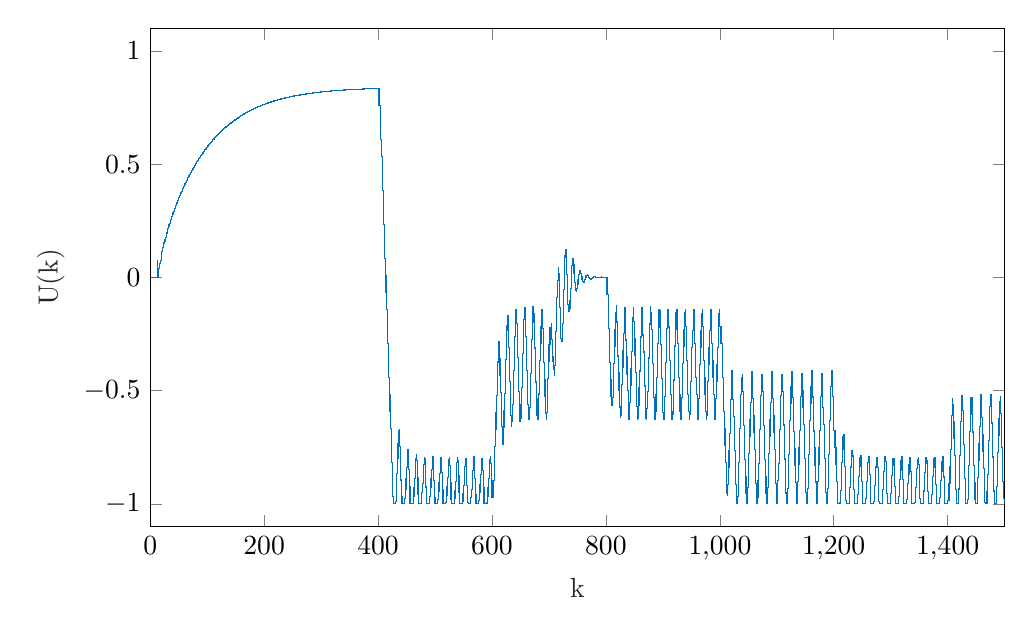
\begin{tikzpicture}

\begin{axis}[%
width=4.272in,
height=2.491in,
at={(0.717in,0.423in)},
scale only axis,
xmin=0,
xmax=1500,
xlabel style={font=\color{white!15!black}},
xlabel={k},
ymin=-1.1,
ymax=1.1,
ylabel style={font=\color{white!15!black}},
ylabel={U(k)},
axis background/.style={fill=white}
]
\addplot[const plot, color=mycolor1, forget plot] table[row sep=crcr] {%
1	0\\
2	0\\
3	0\\
4	0\\
5	0\\
6	0\\
7	0\\
8	0\\
9	0\\
10	0\\
11	0\\
12	0.075\\
13	0\\
14	0.0190628571428573\\
15	0.0381257142857145\\
16	0.0571885714285718\\
17	0.060911330010348\\
18	0.0734168223109094\\
19	0.0978454547477521\\
20	0.112768565666698\\
21	0.122465163713898\\
22	0.132209854150575\\
23	0.143098541219988\\
24	0.151740049214972\\
25	0.158903476099841\\
26	0.167265169651217\\
27	0.176700484580131\\
28	0.186227774025231\\
29	0.195504413653524\\
30	0.204798167566138\\
31	0.213994340796613\\
32	0.222753556332401\\
33	0.231055248800783\\
34	0.239066914416903\\
35	0.246899499361825\\
36	0.254567797259571\\
37	0.26209795712274\\
38	0.269535307169394\\
39	0.276890706357251\\
40	0.28414580831175\\
41	0.291284529933911\\
42	0.298304656678793\\
43	0.30520764661408\\
44	0.311994075391243\\
45	0.318667556499856\\
46	0.325234906234797\\
47	0.331702728696285\\
48	0.338075476412705\\
49	0.34435628725185\\
50	0.350547891136395\\
51	0.356652546244325\\
52	0.362672030455353\\
53	0.368607981943358\\
54	0.374462159562802\\
55	0.380236398498976\\
56	0.385932491982023\\
57	0.39155216620561\\
58	0.397097083592625\\
59	0.402568821935571\\
60	0.407968855460649\\
61	0.413298564418749\\
62	0.418559256296763\\
63	0.423752178437305\\
64	0.4288785242187\\
65	0.433939439245842\\
66	0.438936027099092\\
67	0.443869352260738\\
68	0.448740441339025\\
69	0.453550284698342\\
70	0.458299838686345\\
71	0.46299002782384\\
72	0.46762174682424\\
73	0.472195862627008\\
74	0.476713216397146\\
75	0.48117462531548\\
76	0.485580884132917\\
77	0.489932766562456\\
78	0.494231026551492\\
79	0.498476399437598\\
80	0.502669603000671\\
81	0.506811338435252\\
82	0.510902291255131\\
83	0.514943132131237\\
84	0.518934517664643\\
85	0.522877091099955\\
86	0.526771482983916\\
87	0.530618311772721\\
88	0.534418184391914\\
89	0.53817169675329\\
90	0.541879434232875\\
91	0.545541972113322\\
92	0.549159875993708\\
93	0.552733702169522\\
94	0.556263997985319\\
95	0.559751302162276\\
96	0.563196145102638\\
97	0.566599049172962\\
98	0.569960528967864\\
99	0.573281091555891\\
100	0.576561236708942\\
101	0.579801457116599\\
102	0.583002238586586\\
103	0.586164060232489\\
104	0.589287394649748\\
105	0.592372708080873\\
106	0.595420460570749\\
107	0.598431106112811\\
108	0.601405092786824\\
109	0.604342862888928\\
110	0.607244853054561\\
111	0.610111494374819\\
112	0.612943212506771\\
113	0.615740427778194\\
114	0.61850355528717\\
115	0.621233004996933\\
116	0.623929181826339\\
117	0.626592485736287\\
118	0.629223311812399\\
119	0.631822050344251\\
120	0.634389086901397\\
121	0.636924802406437\\
122	0.639429573205341\\
123	0.641903771135234\\
124	0.644347763589815\\
125	0.646761913582597\\
126	0.649146579808106\\
127	0.651502116701185\\
128	0.653828874494549\\
129	0.656127199274681\\
130	0.658397433036212\\
131	0.660639913734862\\
132	0.662854975339048\\
133	0.665042947880237\\
134	0.667204157502127\\
135	0.669338926508724\\
136	0.671447573411392\\
137	0.673530412974912\\
138	0.67558775626264\\
139	0.677619910680781\\
140	0.679627180021855\\
141	0.681609864507378\\
142	0.683568260829803\\
143	0.685502662193772\\
144	0.687413358356681\\
145	0.689300635668627\\
146	0.691164777111734\\
147	0.693006062338904\\
148	0.694824767712002\\
149	0.696621166339512\\
150	0.698395528113675\\
151	0.700148119747127\\
152	0.701879204809063\\
153	0.703589043760929\\
154	0.705277893991675\\
155	0.706946009852567\\
156	0.708593642691572\\
157	0.710221040887344\\
158	0.711828449882796\\
159	0.713416112218296\\
160	0.714984267564464\\
161	0.716533152754618\\
162	0.718063001816834\\
163	0.719574046005669\\
164	0.72106651383352\\
165	0.722540631101642\\
166	0.723996620930837\\
167	0.725434703791803\\
168	0.726855097535155\\
169	0.728258017421138\\
170	0.729643676149005\\
171	0.731012283886101\\
172	0.732364048296626\\
173	0.733699174570101\\
174	0.735017865449535\\
175	0.73632032125929\\
176	0.737606739932662\\
177	0.738877317039164\\
178	0.740132245811528\\
179	0.741371717172426\\
180	0.742595919760905\\
181	0.743805039958552\\
182	0.744999261915378\\
183	0.746178767575436\\
184	0.747343736702167\\
185	0.748494346903481\\
186	0.749630773656577\\
187	0.750753190332493\\
188	0.751861768220411\\
189	0.75295667655169\\
190	0.754038082523656\\
191	0.75510615132314\\
192	0.756161046149756\\
193	0.757202928238944\\
194	0.758231956884763\\
195	0.759248289462436\\
196	0.760252081450662\\
197	0.761243486453685\\
198	0.76222265622313\\
199	0.763189740679596\\
200	0.764144887934028\\
201	0.765088244308849\\
202	0.76601995435887\\
203	0.76694016089197\\
204	0.767849004989552\\
205	0.768746626026777\\
206	0.769633161692583\\
207	0.770508748009472\\
208	0.771373519353098\\
209	0.772227608471623\\
210	0.773071146504879\\
211	0.7739042630033\\
212	0.774727085946663\\
213	0.775539741762607\\
214	0.776342355344961\\
215	0.777135050071857\\
216	0.777917947823652\\
217	0.778691169000644\\
218	0.77945483254059\\
219	0.78020905593604\\
220	0.780953955251459\\
221	0.781689645140175\\
222	0.782416238861125\\
223	0.78313384829542\\
224	0.783842583962718\\
225	0.784542555037421\\
226	0.785233869364677\\
227	0.785916633476214\\
228	0.786590952605987\\
229	0.78725693070565\\
230	0.787914670459851\\
231	0.788564273301358\\
232	0.789205839426004\\
233	0.789839467807474\\
234	0.790465256211909\\
235	0.791083301212358\\
236	0.791693698203051\\
237	0.792296541413518\\
238	0.792891923922543\\
239	0.793479937671958\\
240	0.794060673480275\\
241	0.794634221056168\\
242	0.795200669011795\\
243	0.795760104875966\\
244	0.796312615107161\\
245	0.796858285106396\\
246	0.797397199229943\\
247	0.797929440801898\\
248	0.798455092126606\\
249	0.798974234500943\\
250	0.79948694822645\\
251	0.799993312621335\\
252	0.800493406032325\\
253	0.800987305846386\\
254	0.801475088502306\\
255	0.80195682950214\\
256	0.802432603422525\\
257	0.802902483925857\\
258	0.803366543771342\\
259	0.80382485482592\\
260	0.804277488075051\\
261	0.804724513633382\\
262	0.805166000755289\\
263	0.805602017845294\\
264	0.806032632468352\\
265	0.806457911360032\\
266	0.806877920436562\\
267	0.807292724804768\\
268	0.807702388771885\\
269	0.808106975855267\\
270	0.808506548791962\\
271	0.808901169548191\\
272	0.809290899328709\\
273	0.80967579858605\\
274	0.810055927029672\\
275	0.810431343634986\\
276	0.810802106652279\\
277	0.811168273615535\\
278	0.81152990135115\\
279	0.811887045986535\\
280	0.812239762958632\\
281	0.812588107022316\\
282	0.8129321322587\\
283	0.813271892083345\\
284	0.813607439254368\\
285	0.813938825880454\\
286	0.814266103428775\\
287	0.814589322732809\\
288	0.814908534000071\\
289	0.81522378681975\\
290	0.815535130170251\\
291	0.815842612426654\\
292	0.816146281368075\\
293	0.816446184184945\\
294	0.816742367486203\\
295	0.817034877306394\\
296	0.817323759112691\\
297	0.817609057811828\\
298	0.817890817756954\\
299	0.818169082754396\\
300	0.81844389607035\\
301	0.818715300437487\\
302	0.81898333806148\\
303	0.819248050627455\\
304	0.819509479306358\\
305	0.81976766476125\\
306	0.820022647153532\\
307	0.820274466149078\\
308	0.820523160924312\\
309	0.820768770172203\\
310	0.821011332108184\\
311	0.821250884476013\\
312	0.821487464553544\\
313	0.821721109158449\\
314	0.821951854653853\\
315	0.82217973695391\\
316	0.822404791529315\\
317	0.822627053412736\\
318	0.822846557204195\\
319	0.823063337076376\\
320	0.823277426779867\\
321	0.823488859648346\\
322	0.823697668603694\\
323	0.823903886161059\\
324	0.824107544433843\\
325	0.824308675138645\\
326	0.824507309600128\\
327	0.82470347875584\\
328	0.82489721316097\\
329	0.825088542993044\\
330	0.825277498056571\\
331	0.825464107787629\\
332	0.825648401258391\\
333	0.825830407181603\\
334	0.826010153915006\\
335	0.826187669465698\\
336	0.82636298149445\\
337	0.82653611731997\\
338	0.826707103923106\\
339	0.826875967951008\\
340	0.827042735721235\\
341	0.82720743322581\\
342	0.827370086135231\\
343	0.827530719802426\\
344	0.827689359266665\\
345	0.827846029257426\\
346	0.828000754198203\\
347	0.828153558210285\\
348	0.828304465116469\\
349	0.828453498444747\\
350	0.828600681431931\\
351	0.828746037027246\\
352	0.828889587895872\\
353	0.829031356422448\\
354	0.829171364714527\\
355	0.829309634605994\\
356	0.829446187660439\\
357	0.829581045174493\\
358	0.829714228181117\\
359	0.829845757452854\\
360	0.829975653505044\\
361	0.830103936598995\\
362	0.830230626745115\\
363	0.830355743706012\\
364	0.830479306999548\\
365	0.830601335901863\\
366	0.830721849450352\\
367	0.830840866446619\\
368	0.830958405459381\\
369	0.83107448482735\\
370	0.831189122662064\\
371	0.831302336850699\\
372	0.831414145058837\\
373	0.831524564733201\\
374	0.831633613104358\\
375	0.831741307189393\\
376	0.83184766379454\\
377	0.831952699517788\\
378	0.832056430751459\\
379	0.83215887368474\\
380	0.832260044306199\\
381	0.832359958406263\\
382	0.832458631579665\\
383	0.832556079227864\\
384	0.832652316561432\\
385	0.832747358602414\\
386	0.832841220186658\\
387	0.83293391596612\\
388	0.83302546041113\\
389	0.833115867812647\\
390	0.833205152284467\\
391	0.833293327765422\\
392	0.833380408021537\\
393	0.833466406648171\\
394	0.833551337072127\\
395	0.833635212553736\\
396	0.833718046188915\\
397	0.833799850911203\\
398	0.833880639493768\\
399	0.833960424551393\\
400	0.83403921854243\\
401	0.75903921854243\\
402	0.83403921854243\\
403	0.75903921854243\\
404	0.68403921854243\\
405	0.60903921854243\\
406	0.53403921854243\\
407	0.45903921854243\\
408	0.38403921854243\\
409	0.30903921854243\\
410	0.23403921854243\\
411	0.15903921854243\\
412	0.0840392185424303\\
413	0.00903921854243026\\
414	-0.0659607814575697\\
415	-0.14096078145757\\
416	-0.21596078145757\\
417	-0.29096078145757\\
418	-0.36596078145757\\
419	-0.44096078145757\\
420	-0.51596078145757\\
421	-0.59096078145757\\
422	-0.66596078145757\\
423	-0.74096078145757\\
424	-0.81596078145757\\
425	-0.89096078145757\\
426	-0.965960781457569\\
427	-1\\
428	-1\\
429	-1\\
430	-1\\
431	-0.991165943250551\\
432	-0.935828964102367\\
433	-0.86785551603819\\
434	-0.799389814676529\\
435	-0.732378520442387\\
436	-0.674950197599703\\
437	-0.670213088675171\\
438	-0.745213088675171\\
439	-0.820213088675171\\
440	-0.895213088675171\\
441	-0.970213088675171\\
442	-1\\
443	-1\\
444	-1\\
445	-1\\
446	-1\\
447	-0.976087814480224\\
448	-0.935650373846095\\
449	-0.890017974251078\\
450	-0.841597535924086\\
451	-0.792105053314593\\
452	-0.762378389995374\\
453	-0.776614543015888\\
454	-0.848525557035062\\
455	-0.923525557035062\\
456	-0.998525557035062\\
457	-1\\
458	-1\\
459	-1\\
460	-1\\
461	-0.999099355447663\\
462	-0.967618672574496\\
463	-0.929559630592471\\
464	-0.887681340784938\\
465	-0.843722159503137\\
466	-0.799661962519824\\
467	-0.782545957725492\\
468	-0.810361849139959\\
469	-0.885361849139959\\
470	-0.960361849139959\\
471	-1\\
472	-1\\
473	-1\\
474	-1\\
475	-1\\
476	-0.984639701982002\\
477	-0.950947902575584\\
478	-0.912276579222211\\
479	-0.870601821347492\\
480	-0.827369026282094\\
481	-0.796410786798216\\
482	-0.799975161605056\\
483	-0.851096418924794\\
484	-0.926096418924794\\
485	-1\\
486	-1\\
487	-1\\
488	-1\\
489	-1\\
490	-0.997619247847291\\
491	-0.966664375638537\\
492	-0.929951447618801\\
493	-0.889625968348482\\
494	-0.847275246372079\\
495	-0.806004941281075\\
496	-0.791803834887639\\
497	-0.821191760438776\\
498	-0.896191760438776\\
499	-0.971191760438776\\
500	-1\\
501	-1\\
502	-1\\
503	-1\\
504	-1\\
505	-0.980680449852594\\
506	-0.946520030247978\\
507	-0.907771473770955\\
508	-0.866279271525097\\
509	-0.823389505322068\\
510	-0.796259449738358\\
511	-0.805628063378586\\
512	-0.863131950950039\\
513	-0.938131950950039\\
514	-1\\
515	-1\\
516	-1\\
517	-1\\
518	-1\\
519	-0.993169013924011\\
520	-0.961446207778469\\
521	-0.924284230319871\\
522	-0.883741124792812\\
523	-0.841335186641125\\
524	-0.803816830410649\\
525	-0.795767605573364\\
526	-0.832389273897231\\
527	-0.907389273897231\\
528	-0.982389273897231\\
529	-1\\
530	-1\\
531	-1\\
532	-1\\
533	-1\\
534	-0.976239043393215\\
535	-0.941173087589295\\
536	-0.901897333425864\\
537	-0.860152218828665\\
538	-0.817201773588742\\
539	-0.79396646107419\\
540	-0.809799842199516\\
541	-0.874991589859039\\
542	-0.949991589859039\\
543	-1\\
544	-1\\
545	-1\\
546	-1\\
547	-1\\
548	-0.988760733867632\\
549	-0.956215292262508\\
550	-0.918520273688861\\
551	-0.877660702341668\\
552	-0.835096060794947\\
553	-0.801223066080323\\
554	-0.799255371911692\\
555	-0.843137246670607\\
556	-0.918137246670607\\
557	-0.993137246670607\\
558	-1\\
559	-1\\
560	-1\\
561	-1\\
562	-1\\
563	-0.971962842909188\\
564	-0.936006216760714\\
565	-0.896198558865376\\
566	-0.854183273203191\\
567	-0.811147568135787\\
568	-0.79167048758145\\
569	-0.813762298454948\\
570	-0.886422276743108\\
571	-0.961422276743108\\
572	-1\\
573	-1\\
574	-1\\
575	-1\\
576	-1\\
577	-0.984519400491059\\
578	-0.951182381994481\\
579	-0.912970787871608\\
580	-0.871800834726858\\
581	-0.82907647640652\\
582	-0.798731716533256\\
583	-0.80264238114429\\
584	-0.853541355326907\\
585	-0.928541355326907\\
586	-1\\
587	-1\\
588	-1\\
589	-1\\
590	-1\\
591	-0.996761468976097\\
592	-0.965736539764808\\
593	-0.929039878482044\\
594	-0.888786260445464\\
595	-0.84654006260055\\
596	-0.806101753721948\\
597	-0.793127910670741\\
598	-0.823825557425575\\
599	-0.898825557425575\\
600	-0.973825557425575\\
601	-0.898825557425575\\
602	-0.973825557425575\\
603	-0.898825557425575\\
604	-0.823825557425575\\
605	-0.748825557425575\\
606	-0.673825557425575\\
607	-0.598825557425575\\
608	-0.523825557425575\\
609	-0.448825557425575\\
610	-0.373825557425575\\
611	-0.298825557425575\\
612	-0.285424849770675\\
613	-0.360424849770675\\
614	-0.435424849770675\\
615	-0.510424849770675\\
616	-0.585424849770675\\
617	-0.660424849770675\\
618	-0.735424849770675\\
619	-0.736991087553225\\
620	-0.661991087553225\\
621	-0.586991087553225\\
622	-0.511991087553226\\
623	-0.436991087553226\\
624	-0.361991087553226\\
625	-0.286991087553225\\
626	-0.211991087553225\\
627	-0.170560708838591\\
628	-0.235649004995078\\
629	-0.310649004995078\\
630	-0.385649004995078\\
631	-0.460649004995078\\
632	-0.535649004995078\\
633	-0.610649004995078\\
634	-0.657938845144998\\
635	-0.636298382234271\\
636	-0.561298382234271\\
637	-0.486298382234271\\
638	-0.411298382234271\\
639	-0.336298382234271\\
640	-0.261298382234271\\
641	-0.186298382234271\\
642	-0.143017667814511\\
643	-0.204708915495589\\
644	-0.279708915495589\\
645	-0.354708915495589\\
646	-0.429708915495589\\
647	-0.504708915495589\\
648	-0.579708915495589\\
649	-0.634687290307433\\
650	-0.625360762575771\\
651	-0.562056170542463\\
652	-0.487056170542463\\
653	-0.412056170542463\\
654	-0.337056170542463\\
655	-0.262056170542463\\
656	-0.187056170542463\\
657	-0.134811523195165\\
658	-0.187005097473413\\
659	-0.262005097473413\\
660	-0.337005097473413\\
661	-0.412005097473413\\
662	-0.487005097473413\\
663	-0.562005097473413\\
664	-0.627499070525412\\
665	-0.628077029569525\\
666	-0.575144366012471\\
667	-0.500144366012471\\
668	-0.425144366012471\\
669	-0.350144366012471\\
670	-0.275144366012471\\
671	-0.200144366012471\\
672	-0.128987989387914\\
673	-0.162026868513731\\
674	-0.237026868513731\\
675	-0.312026868513731\\
676	-0.387026868513731\\
677	-0.462026868513731\\
678	-0.537026868513731\\
679	-0.612026868513731\\
680	-0.628305899853729\\
681	-0.590444202799664\\
682	-0.515444202799664\\
683	-0.440444202799664\\
684	-0.365444202799664\\
685	-0.290444202799664\\
686	-0.215444202799664\\
687	-0.140444202799664\\
688	-0.149587811060605\\
689	-0.224587811060605\\
690	-0.299587811060605\\
691	-0.374587811060605\\
692	-0.449587811060605\\
693	-0.524587811060605\\
694	-0.599587811060605\\
695	-0.626981286713882\\
696	-0.598298193276153\\
697	-0.523298193276153\\
698	-0.448298193276153\\
699	-0.373298193276153\\
700	-0.298298193276153\\
701	-0.223298193276153\\
702	-0.298298193276153\\
703	-0.223298193276153\\
704	-0.20399479245519\\
705	-0.275979199514718\\
706	-0.350979199514718\\
707	-0.373611582155224\\
708	-0.406252694771342\\
709	-0.432492084893234\\
710	-0.387501539350272\\
711	-0.312501539350272\\
712	-0.237501539350272\\
713	-0.162501539350272\\
714	-0.0875015393502722\\
715	-0.0125015393502722\\
716	0.0445757660504938\\
717	0.0182814155207235\\
718	-0.0567185844792765\\
719	-0.131718584479277\\
720	-0.206718584479277\\
721	-0.26909556761307\\
722	-0.282670927307244\\
723	-0.257807053615104\\
724	-0.202241276539699\\
725	-0.127241276539699\\
726	-0.0522412765396992\\
727	0.0227587234603008\\
728	0.0977587234603008\\
729	0.124426024939221\\
730	0.0882601615233711\\
731	0.0135028298941955\\
732	-0.0614971701058045\\
733	-0.1203820558473\\
734	-0.148417189860917\\
735	-0.152268301116481\\
736	-0.13686950968022\\
737	-0.10190520386809\\
738	-0.0507326844162345\\
739	0.0054562829221971\\
740	0.0525526773974103\\
741	0.080366654209796\\
742	0.0819368304225889\\
743	0.0569328212286605\\
744	0.0166829447910366\\
745	-0.0216734571223702\\
746	-0.0476402895782855\\
747	-0.0599060312628958\\
748	-0.0605079629815263\\
749	-0.0506700236550083\\
750	-0.0321831885711123\\
751	-0.00963853395458437\\
752	0.0111918063852153\\
753	0.025862772795786\\
754	0.0317588942685523\\
755	0.0282230343527133\\
756	0.0173555975907334\\
757	0.003457883057661\\
758	-0.00920337731823761\\
759	-0.0179812482655135\\
760	-0.0218528120327427\\
761	-0.0208609033365961\\
762	-0.0158598815601308\\
763	-0.00842487909268626\\
764	-0.000509635281678847\\
765	0.00606284380117591\\
766	0.00999217525629154\\
767	0.0107313036947778\\
768	0.0085790539120915\\
769	0.00453483984253604\\
770	-9.19143903279004e-05\\
771	-0.00410924790060873\\
772	-0.00670794035028947\\
773	-0.00754288718719813\\
774	-0.00670412790609645\\
775	-0.00462614798516648\\
776	-0.00194952235793511\\
777	0.000643724177127165\\
778	0.00258528756517712\\
779	0.00353471677000979\\
780	0.00343101804733652\\
781	0.00247061152459509\\
782	0.00102076182204821\\
783	-0.000498532921616515\\
784	-0.00172372684526418\\
785	-0.00242069679759613\\
786	-0.00251347778785252\\
787	-0.00207358038063948\\
788	-0.00128027106814199\\
789	-0.000364466018708006\\
790	0.000450279118255328\\
791	0.000997074858171436\\
792	0.00119561747618985\\
793	0.00105795160222325\\
794	0.000671536886384009\\
795	0.000166894746999153\\
796	-0.000319698682965596\\
797	-0.000678486000710847\\
798	-0.000846767760368211\\
799	-0.00081524692009246\\
800	-0.000621398841104449\\
801	-0.0756213988411044\\
802	-0.000621398841104445\\
803	-0.0756213988411044\\
804	-0.150621398841104\\
805	-0.225621398841104\\
806	-0.300621398841104\\
807	-0.375621398841104\\
808	-0.450621398841104\\
809	-0.524079813505627\\
810	-0.563686645007485\\
811	-0.567100775773322\\
812	-0.53050698147014\\
813	-0.45550698147014\\
814	-0.38050698147014\\
815	-0.30550698147014\\
816	-0.23050698147014\\
817	-0.15550698147014\\
818	-0.125508068939682\\
819	-0.197517460674661\\
820	-0.272517460674661\\
821	-0.347517460674661\\
822	-0.422517460674661\\
823	-0.497517460674661\\
824	-0.572517460674661\\
825	-0.619439967373935\\
826	-0.608268494054294\\
827	-0.546443441169408\\
828	-0.471443441169408\\
829	-0.396443441169408\\
830	-0.321443441169408\\
831	-0.246443441169408\\
832	-0.171443441169408\\
833	-0.13463359598715\\
834	-0.201698090679743\\
835	-0.276698090679743\\
836	-0.351698090679743\\
837	-0.426698090679743\\
838	-0.501698090679743\\
839	-0.576698090679743\\
840	-0.627377081990724\\
841	-0.616808715364934\\
842	-0.553886491953839\\
843	-0.478886491953839\\
844	-0.403886491953839\\
845	-0.328886491953839\\
846	-0.253886491953839\\
847	-0.178886491953839\\
848	-0.134924647386935\\
849	-0.195149416711073\\
850	-0.270149416711073\\
851	-0.345149416711073\\
852	-0.420149416711073\\
853	-0.495149416711073\\
854	-0.570149416711073\\
855	-0.627592016990342\\
856	-0.622103518245761\\
857	-0.563711044360397\\
858	-0.488711044360397\\
859	-0.413711044360397\\
860	-0.338711044360397\\
861	-0.263711044360397\\
862	-0.188711044360397\\
863	-0.132148031934806\\
864	-0.179843402044301\\
865	-0.254843402044301\\
866	-0.329843402044301\\
867	-0.404843402044301\\
868	-0.479843402044301\\
869	-0.554843402044301\\
870	-0.62506169228962\\
871	-0.629803072386028\\
872	-0.58108883569084\\
873	-0.50608883569084\\
874	-0.43108883569084\\
875	-0.35608883569084\\
876	-0.28108883569084\\
877	-0.20608883569084\\
878	-0.13108883569084\\
879	-0.155771010940138\\
880	-0.230771010940138\\
881	-0.305771010940138\\
882	-0.380771010940138\\
883	-0.455771010940138\\
884	-0.530771010940138\\
885	-0.605771010940138\\
886	-0.626789841853923\\
887	-0.593068846953178\\
888	-0.518068846953178\\
889	-0.443068846953178\\
890	-0.368068846953178\\
891	-0.293068846953178\\
892	-0.218068846953178\\
893	-0.143068846953178\\
894	-0.147372336713507\\
895	-0.222372336713507\\
896	-0.297372336713507\\
897	-0.372372336713507\\
898	-0.447372336713507\\
899	-0.522372336713507\\
900	-0.597372336713507\\
901	-0.626826943910484\\
902	-0.59982822937068\\
903	-0.52482822937068\\
904	-0.44982822937068\\
905	-0.37482822937068\\
906	-0.29982822937068\\
907	-0.22482822937068\\
908	-0.14982822937068\\
909	-0.1442334752874\\
910	-0.2192334752874\\
911	-0.2942334752874\\
912	-0.3692334752874\\
913	-0.4442334752874\\
914	-0.5192334752874\\
915	-0.5942334752874\\
916	-0.627569424193558\\
917	-0.603433171610519\\
918	-0.52843317161052\\
919	-0.453433171610519\\
920	-0.378433171610519\\
921	-0.303433171610519\\
922	-0.228433171610519\\
923	-0.153433171610519\\
924	-0.14295997740128\\
925	-0.21795997740128\\
926	-0.29295997740128\\
927	-0.36795997740128\\
928	-0.44295997740128\\
929	-0.51795997740128\\
930	-0.59295997740128\\
931	-0.628158057462986\\
932	-0.605324361646243\\
933	-0.531118748775727\\
934	-0.456118748775727\\
935	-0.381118748775727\\
936	-0.306118748775727\\
937	-0.231118748775727\\
938	-0.156118748775727\\
939	-0.142246806900678\\
940	-0.217246806900678\\
941	-0.292246806900678\\
942	-0.367246806900678\\
943	-0.442246806900678\\
944	-0.517246806900678\\
945	-0.592246806900678\\
946	-0.628704448271995\\
947	-0.60670876226052\\
948	-0.533154155030121\\
949	-0.458154155030121\\
950	-0.383154155030121\\
951	-0.308154155030121\\
952	-0.23315415503012\\
953	-0.15815415503012\\
954	-0.141774495760927\\
955	-0.216774495760927\\
956	-0.291774495760927\\
957	-0.366774495760927\\
958	-0.441774495760927\\
959	-0.516774495760927\\
960	-0.591774495760927\\
961	-0.629153277968245\\
962	-0.607755994581573\\
963	-0.534654088996682\\
964	-0.459654088996682\\
965	-0.384654088996682\\
966	-0.309654088996682\\
967	-0.234654088996681\\
968	-0.159654088996681\\
969	-0.141444880685857\\
970	-0.216444880685857\\
971	-0.291444880685857\\
972	-0.366444880685857\\
973	-0.441444880685857\\
974	-0.516444880685857\\
975	-0.591444880685857\\
976	-0.629494993656054\\
977	-0.608529451789189\\
978	-0.535750432862366\\
979	-0.460750432862366\\
980	-0.385750432862366\\
981	-0.310750432862366\\
982	-0.235750432862366\\
983	-0.160750432862366\\
984	-0.141209918094215\\
985	-0.216209918094215\\
986	-0.291209918094215\\
987	-0.366209918094215\\
988	-0.441209918094215\\
989	-0.516209918094215\\
990	-0.591209918094215\\
991	-0.629748856326679\\
992	-0.609096145556347\\
993	-0.536549769531562\\
994	-0.461549769531562\\
995	-0.386549769531562\\
996	-0.311549769531562\\
997	-0.236549769531562\\
998	-0.161549769531562\\
999	-0.141040902080289\\
1000	-0.216040902080289\\
1001	-0.291040902080289\\
1002	-0.216040902080289\\
1003	-0.291040902080289\\
1004	-0.366040902080289\\
1005	-0.441040902080289\\
1006	-0.516040902080289\\
1007	-0.591040902080289\\
1008	-0.666040902080289\\
1009	-0.741040902080288\\
1010	-0.816040902080288\\
1011	-0.891040902080288\\
1012	-0.956135747092132\\
1013	-0.96538600064279\\
1014	-0.915569676352604\\
1015	-0.840569676352604\\
1016	-0.765569676352604\\
1017	-0.690569676352604\\
1018	-0.615569676352604\\
1019	-0.540569676352604\\
1020	-0.465569676352604\\
1021	-0.409919035335093\\
1022	-0.463257787917502\\
1023	-0.538257787917502\\
1024	-0.613257787917502\\
1025	-0.688257787917502\\
1026	-0.763257787917502\\
1027	-0.838257787917502\\
1028	-0.913257787917502\\
1029	-0.988257787917502\\
1030	-1\\
1031	-0.967101313281544\\
1032	-0.892101313281544\\
1033	-0.817101313281544\\
1034	-0.742101313281544\\
1035	-0.667101313281544\\
1036	-0.592101313281544\\
1037	-0.517101313281544\\
1038	-0.442101313281544\\
1039	-0.42998843978431\\
1040	-0.50498843978431\\
1041	-0.57998843978431\\
1042	-0.65498843978431\\
1043	-0.72998843978431\\
1044	-0.80498843978431\\
1045	-0.87998843978431\\
1046	-0.95498843978431\\
1047	-1\\
1048	-1\\
1049	-0.927733757167451\\
1050	-0.852733757167451\\
1051	-0.777733757167451\\
1052	-0.702733757167451\\
1053	-0.627733757167452\\
1054	-0.552733757167452\\
1055	-0.477733757167452\\
1056	-0.415277818853121\\
1057	-0.461565056221945\\
1058	-0.536565056221945\\
1059	-0.611565056221945\\
1060	-0.686565056221945\\
1061	-0.761565056221945\\
1062	-0.836565056221945\\
1063	-0.911565056221945\\
1064	-0.986565056221945\\
1065	-1\\
1066	-0.970535514212989\\
1067	-0.895535514212989\\
1068	-0.82053551421299\\
1069	-0.74553551421299\\
1070	-0.67053551421299\\
1071	-0.59553551421299\\
1072	-0.52053551421299\\
1073	-0.44553551421299\\
1074	-0.428614618528861\\
1075	-0.503614618528861\\
1076	-0.578614618528861\\
1077	-0.65361461852886\\
1078	-0.72861461852886\\
1079	-0.80361461852886\\
1080	-0.87861461852886\\
1081	-0.95361461852886\\
1082	-1\\
1083	-1\\
1084	-0.929330870139078\\
1085	-0.854330870139078\\
1086	-0.779330870139078\\
1087	-0.704330870139078\\
1088	-0.629330870139079\\
1089	-0.554330870139079\\
1090	-0.479330870139079\\
1091	-0.414703458843609\\
1092	-0.458652669572555\\
1093	-0.533652669572555\\
1094	-0.608652669572555\\
1095	-0.683652669572555\\
1096	-0.758652669572555\\
1097	-0.833652669572555\\
1098	-0.908652669572555\\
1099	-0.983652669572555\\
1100	-1\\
1101	-0.973287270576943\\
1102	-0.898287270576943\\
1103	-0.823287270576943\\
1104	-0.748287270576943\\
1105	-0.673287270576943\\
1106	-0.598287270576943\\
1107	-0.523287270576943\\
1108	-0.448287270576943\\
1109	-0.427329395094055\\
1110	-0.502329395094055\\
1111	-0.577329395094055\\
1112	-0.652329395094055\\
1113	-0.727329395094055\\
1114	-0.802329395094055\\
1115	-0.877329395094055\\
1116	-0.952329395094055\\
1117	-1\\
1118	-1\\
1119	-0.930776837420698\\
1120	-0.855776837420698\\
1121	-0.780776837420698\\
1122	-0.705776837420699\\
1123	-0.630776837420699\\
1124	-0.555776837420699\\
1125	-0.480776837420699\\
1126	-0.414177272994487\\
1127	-0.456004147808545\\
1128	-0.531004147808545\\
1129	-0.606004147808545\\
1130	-0.681004147808545\\
1131	-0.756004147808545\\
1132	-0.831004147808545\\
1133	-0.906004147808545\\
1134	-0.981004147808545\\
1135	-1\\
1136	-0.975784597069512\\
1137	-0.900784597069512\\
1138	-0.825784597069512\\
1139	-0.750784597069512\\
1140	-0.675784597069512\\
1141	-0.600784597069512\\
1142	-0.525784597069512\\
1143	-0.450784597069512\\
1144	-0.42617346706259\\
1145	-0.50117346706259\\
1146	-0.57617346706259\\
1147	-0.651173467062589\\
1148	-0.726173467062589\\
1149	-0.801173467062589\\
1150	-0.876173467062589\\
1151	-0.951173467062589\\
1152	-1\\
1153	-1\\
1154	-0.932079563945854\\
1155	-0.857079563945854\\
1156	-0.782079563945854\\
1157	-0.707079563945854\\
1158	-0.632079563945854\\
1159	-0.557079563945854\\
1160	-0.482079563945854\\
1161	-0.413706471495848\\
1162	-0.453624026456548\\
1163	-0.528624026456548\\
1164	-0.603624026456548\\
1165	-0.678624026456548\\
1166	-0.753624026456548\\
1167	-0.828624026456548\\
1168	-0.903624026456548\\
1169	-0.978624026456548\\
1170	-1\\
1171	-0.978025641311212\\
1172	-0.903025641311212\\
1173	-0.828025641311212\\
1174	-0.753025641311212\\
1175	-0.678025641311212\\
1176	-0.603025641311212\\
1177	-0.528025641311212\\
1178	-0.453025641311212\\
1179	-0.425144776776128\\
1180	-0.500144776776128\\
1181	-0.575144776776128\\
1182	-0.650144776776128\\
1183	-0.725144776776128\\
1184	-0.800144776776128\\
1185	-0.875144776776128\\
1186	-0.950144776776128\\
1187	-1\\
1188	-1\\
1189	-0.933240738908566\\
1190	-0.858240738908566\\
1191	-0.783240738908566\\
1192	-0.708240738908567\\
1193	-0.633240738908567\\
1194	-0.558240738908567\\
1195	-0.483240738908567\\
1196	-0.413289433712585\\
1197	-0.451507352635287\\
1198	-0.526507352635287\\
1199	-0.601507352635287\\
1200	-0.676507352635287\\
1201	-0.751507352635287\\
1202	-0.676507352635287\\
1203	-0.751507352635287\\
1204	-0.826507352635287\\
1205	-0.901507352635287\\
1206	-0.976507352635287\\
1207	-1\\
1208	-1\\
1209	-1\\
1210	-1\\
1211	-0.992713515418567\\
1212	-0.942931106891811\\
1213	-0.882123445401616\\
1214	-0.819645815669805\\
1215	-0.757546333662955\\
1216	-0.702887485280812\\
1217	-0.694819269708035\\
1218	-0.761941441166332\\
1219	-0.836941441166332\\
1220	-0.911941441166332\\
1221	-0.986941441166332\\
1222	-1\\
1223	-1\\
1224	-1\\
1225	-1\\
1226	-1\\
1227	-0.970445257548185\\
1228	-0.92994850582217\\
1229	-0.884952495626551\\
1230	-0.83759063672687\\
1231	-0.78937853433788\\
1232	-0.765939649263682\\
1233	-0.788813216889556\\
1234	-0.863813216889555\\
1235	-0.938813216889555\\
1236	-1\\
1237	-1\\
1238	-1\\
1239	-1\\
1240	-1\\
1241	-0.992389565233303\\
1242	-0.959561638395293\\
1243	-0.921017790690316\\
1244	-0.878982627374048\\
1245	-0.835088958465755\\
1246	-0.79677299538923\\
1247	-0.789175698558019\\
1248	-0.828036017080872\\
1249	-0.903036017080872\\
1250	-0.978036017080872\\
1251	-1\\
1252	-1\\
1253	-1\\
1254	-1\\
1255	-1\\
1256	-0.977639427543748\\
1257	-0.942537896980347\\
1258	-0.90305923502909\\
1259	-0.861012216073257\\
1260	-0.817710605078442\\
1261	-0.792873716157953\\
1262	-0.806589659013833\\
1263	-0.869765021940306\\
1264	-0.944765021940306\\
1265	-1\\
1266	-1\\
1267	-1\\
1268	-1\\
1269	-1\\
1270	-0.990671810903773\\
1271	-0.95842017094209\\
1272	-0.920870612387197\\
1273	-0.88005209153998\\
1274	-0.837458150844857\\
1275	-0.801903416065748\\
1276	-0.797250666224093\\
1277	-0.838041144599416\\
1278	-0.913041144599416\\
1279	-0.988041144599416\\
1280	-1\\
1281	-1\\
1282	-1\\
1283	-1\\
1284	-1\\
1285	-0.973966646847418\\
1286	-0.938404817818907\\
1287	-0.898820790853152\\
1288	-0.856905806722797\\
1289	-0.81388465420656\\
1290	-0.792616577188705\\
1291	-0.81176567396315\\
1292	-0.88094996902171\\
1293	-0.95594996902171\\
1294	-1\\
1295	-1\\
1296	-1\\
1297	-1\\
1298	-1\\
1299	-0.986546667677624\\
1300	-0.953583181744053\\
1301	-0.915612303448543\\
1302	-0.874583930193031\\
1303	-0.831929104895829\\
1304	-0.799887611119212\\
1305	-0.800981614777812\\
1306	-0.848527223992035\\
1307	-0.923527223992035\\
1308	-0.998527223992035\\
1309	-1\\
1310	-1\\
1311	-1\\
1312	-1\\
1313	-0.999777284969798\\
1314	-0.969597018087883\\
1315	-0.933193118757994\\
1316	-0.893116851355572\\
1317	-0.850963488119814\\
1318	-0.808065651019428\\
1319	-0.790746363375229\\
1320	-0.816268571206914\\
1321	-0.891268571206914\\
1322	-0.966268571206914\\
1323	-1\\
1324	-1\\
1325	-1\\
1326	-1\\
1327	-1\\
1328	-0.982692306708075\\
1329	-0.948993064085486\\
1330	-0.910538683724955\\
1331	-0.869216440928981\\
1332	-0.826406740620597\\
1333	-0.797575669903176\\
1334	-0.804034859465173\\
1335	-0.858001732717862\\
1336	-0.933001732717861\\
1337	-1\\
1338	-1\\
1339	-1\\
1340	-1\\
1341	-1\\
1342	-0.995082938040154\\
1343	-0.963727331964628\\
1344	-0.926809543144354\\
1345	-0.886417721999714\\
1346	-0.844094598197563\\
1347	-0.805016444492031\\
1348	-0.794343252507156\\
1349	-0.827813822403579\\
1350	-0.902813822403579\\
1351	-0.977813822403579\\
1352	-1\\
1353	-1\\
1354	-1\\
1355	-1\\
1356	-1\\
1357	-0.97806574406944\\
1358	-0.943384607174991\\
1359	-0.904340229830195\\
1360	-0.862714351919558\\
1361	-0.819803739463988\\
1362	-0.794976824881959\\
1363	-0.808149125272647\\
1364	-0.870157579441418\\
1365	-0.945157579441418\\
1366	-1\\
1367	-1\\
1368	-1\\
1369	-1\\
1370	-1\\
1371	-0.990557518023572\\
1372	-0.958349303769714\\
1373	-0.920874655312713\\
1374	-0.880147791479586\\
1375	-0.837651764337795\\
1376	-0.802293280858767\\
1377	-0.797844708809482\\
1378	-0.838761476862817\\
1379	-0.913761476862817\\
1380	-0.988761476862817\\
1381	-1\\
1382	-1\\
1383	-1\\
1384	-1\\
1385	-1\\
1386	-0.973703486897495\\
1387	-0.938109825772219\\
1388	-0.898519480481295\\
1389	-0.856615178843426\\
1390	-0.813615275025926\\
1391	-0.792605354618462\\
1392	-0.812145210300907\\
1393	-0.881759687610406\\
1394	-0.956759687610406\\
1395	-1\\
1396	-1\\
1397	-1\\
1398	-1\\
1399	-1\\
1400	-0.98624839815617\\
1401	-0.91124839815617\\
1402	-0.98624839815617\\
1403	-0.91124839815617\\
1404	-0.83624839815617\\
1405	-0.76124839815617\\
1406	-0.68624839815617\\
1407	-0.61124839815617\\
1408	-0.536910822736744\\
1409	-0.56024380316925\\
1410	-0.63524380316925\\
1411	-0.71024380316925\\
1412	-0.785243803169249\\
1413	-0.860243803169249\\
1414	-0.935243803169249\\
1415	-1\\
1416	-1\\
1417	-1\\
1418	-1\\
1419	-0.934977862157578\\
1420	-0.859977862157578\\
1421	-0.784977862157578\\
1422	-0.709977862157578\\
1423	-0.634977862157578\\
1424	-0.559977862157578\\
1425	-0.523432915149657\\
1426	-0.589483690568054\\
1427	-0.664483690568054\\
1428	-0.739483690568054\\
1429	-0.814483690568053\\
1430	-0.889483690568053\\
1431	-0.964483690568053\\
1432	-1\\
1433	-1\\
1434	-1\\
1435	-0.980969113551293\\
1436	-0.905969113551293\\
1437	-0.830969113551293\\
1438	-0.755969113551293\\
1439	-0.680969113551293\\
1440	-0.605969113551293\\
1441	-0.530969113551293\\
1442	-0.532914451042424\\
1443	-0.607914451042424\\
1444	-0.682914451042424\\
1445	-0.757914451042424\\
1446	-0.832914451042424\\
1447	-0.907914451042424\\
1448	-0.982914451042424\\
1449	-1\\
1450	-1\\
1451	-1\\
1452	-0.960407290681765\\
1453	-0.885407290681765\\
1454	-0.810407290681765\\
1455	-0.735407290681765\\
1456	-0.660407290681765\\
1457	-0.585407290681765\\
1458	-0.51581313182921\\
1459	-0.545577089188483\\
1460	-0.620577089188483\\
1461	-0.695577089188482\\
1462	-0.770577089188482\\
1463	-0.845577089188482\\
1464	-0.920577089188482\\
1465	-0.995577089188482\\
1466	-1\\
1467	-1\\
1468	-1\\
1469	-0.946331240581299\\
1470	-0.871331240581299\\
1471	-0.796331240581299\\
1472	-0.721331240581299\\
1473	-0.646331240581299\\
1474	-0.571331240581299\\
1475	-0.519264932197595\\
1476	-0.56853377294414\\
1477	-0.64353377294414\\
1478	-0.71853377294414\\
1479	-0.79353377294414\\
1480	-0.86853377294414\\
1481	-0.94353377294414\\
1482	-1\\
1483	-1\\
1484	-1\\
1485	-1\\
1486	-0.925\\
1487	-0.85\\
1488	-0.775\\
1489	-0.7\\
1490	-0.625\\
1491	-0.55\\
1492	-0.525996119343033\\
1493	-0.600996119343033\\
1494	-0.675996119343033\\
1495	-0.750996119343033\\
1496	-0.825996119343033\\
1497	-0.900996119343033\\
1498	-0.975996119343033\\
1499	-1\\
1500	-1\\
};
\end{axis}
\end{tikzpicture}%
\caption{Sterowanie, $K = 1,6680; T_i=3,5; T_d=0,84;$}
\end{figure}

\subsection{Dostrojenie metodą inżynierską}

Zmniejszymy $K$ do 1 żeby zmniejszyć oscylacje:

\begin{figure}[H]
\centering
% This file was created by matlab2tikz.
%
%The latest updates can be retrieved from
%  http://www.mathworks.com/matlabcentral/fileexchange/22022-matlab2tikz-matlab2tikz
%where you can also make suggestions and rate matlab2tikz.
%
\definecolor{mycolor1}{rgb}{0.00000,0.44700,0.74100}%
\definecolor{mycolor2}{rgb}{0.85000,0.32500,0.09800}%
%
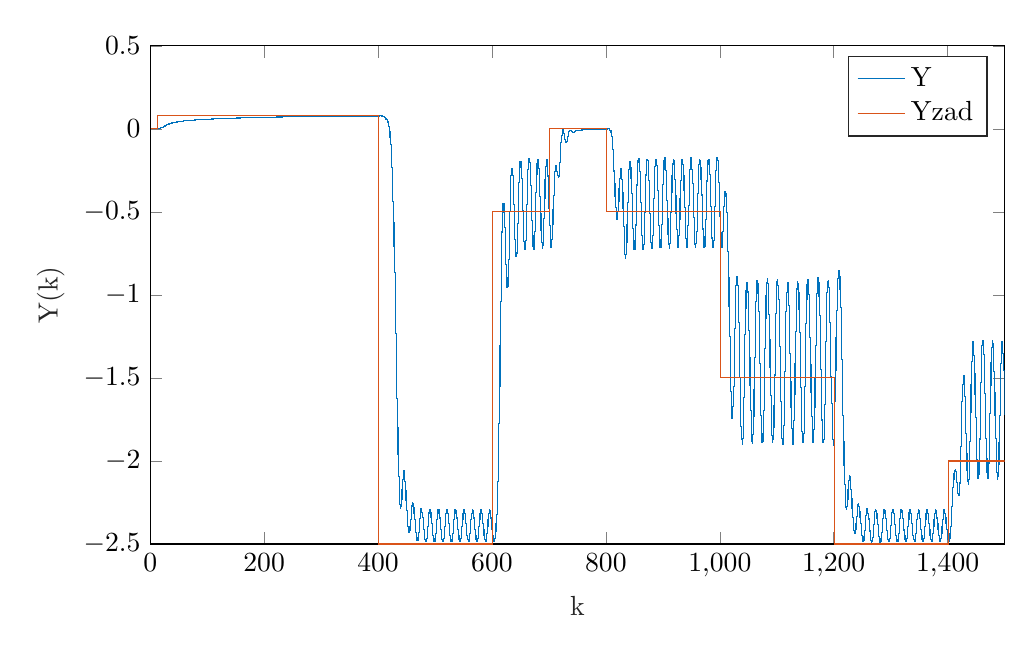
\begin{tikzpicture}

\begin{axis}[%
width=4.272in,
height=2.491in,
at={(0.717in,0.423in)},
scale only axis,
xmin=0,
xmax=1500,
xlabel style={font=\color{white!15!black}},
xlabel={k},
ymin=-2.5,
ymax=0.5,
ylabel style={font=\color{white!15!black}},
ylabel={Y(k)},
axis background/.style={fill=white},
legend style={legend cell align=left, align=left, draw=white!15!black}
]
\addplot[const plot, color=mycolor1] table[row sep=crcr] {%
1	0\\
2	0\\
3	0\\
4	0\\
5	0\\
6	0\\
7	0\\
8	0\\
9	0\\
10	0\\
11	0\\
12	0\\
13	0\\
14	0\\
15	0\\
16	0\\
17	0.00334251881758044\\
18	0.00663869844795659\\
19	0.00681604409833907\\
20	0.00671148782284413\\
21	0.0074189846133044\\
22	0.00873453116724653\\
23	0.0102996582738255\\
24	0.0123697024632401\\
25	0.0149612408563968\\
26	0.017658903591963\\
27	0.0201618732945124\\
28	0.0223872377212654\\
29	0.0243367738754835\\
30	0.0260119830851231\\
31	0.0274529476542554\\
32	0.028738438855228\\
33	0.0299355010612659\\
34	0.0310789968183597\\
35	0.0321818786637987\\
36	0.0332473424026577\\
37	0.0342718456610686\\
38	0.035248315294456\\
39	0.0361715706303644\\
40	0.0370409044329503\\
41	0.0378591633101956\\
42	0.038630909606235\\
43	0.039361256071456\\
44	0.0400551149358091\\
45	0.040716613896036\\
46	0.0413488842718455\\
47	0.0419542296851506\\
48	0.0425344291061038\\
49	0.0430909772695488\\
50	0.0436252345476058\\
51	0.0441385120453321\\
52	0.0446321011069905\\
53	0.0451072608907354\\
54	0.0455651906561502\\
55	0.046007008431965\\
56	0.0464337420148742\\
57	0.0468463296041299\\
58	0.0472456266541333\\
59	0.0476324159707084\\
60	0.0480074181436993\\
61	0.0483713002785418\\
62	0.0487246824819577\\
63	0.0490681425256726\\
64	0.0494022193037399\\
65	0.0497274155854599\\
66	0.0500442004310262\\
67	0.0503530114922092\\
68	0.0506542572701338\\
69	0.0509483193058036\\
70	0.0512355542548079\\
71	0.051516295811102\\
72	0.0517908564642449\\
73	0.0520595290907805\\
74	0.0523225883926759\\
75	0.0525802922019607\\
76	0.05283288267075\\
77	0.0530805873625045\\
78	0.0533236202566306\\
79	0.0535621826755395\\
80	0.053796464141181\\
81	0.0540266431667581\\
82	0.0542528879886487\\
83	0.0544753572432372\\
84	0.0546942005931344\\
85	0.0549095593070036\\
86	0.0551215667969114\\
87	0.0553303491167917\\
88	0.0555360254252744\\
89	0.0557387084158096\\
90	0.0559385047167253\\
91	0.0561355152636021\\
92	0.056329835646129\\
93	0.0565215564314075\\
94	0.0567107634655044\\
95	0.0568975381548954\\
96	0.05708195772931\\
97	0.0572640954873539\\
98	0.0574440210261785\\
99	0.0576218004563557\\
100	0.0577974966030255\\
101	0.057971169194294\\
102	0.0581428750377843\\
103	0.0583126681861665\\
104	0.058480600092433\\
105	0.058646719755622\\
106	0.0588110738576391\\
107	0.0589737068917788\\
108	0.0591346612834994\\
109	0.0592939775039668\\
110	0.0594516941768413\\
111	0.0596078481787492\\
112	0.0597624747338472\\
113	0.0599156075028597\\
114	0.0600672786669407\\
115	0.0602175190066872\\
116	0.0603663579766099\\
117	0.0605138237753428\\
118	0.0606599434118566\\
119	0.0608047427679212\\
120	0.0609482466570461\\
121	0.0610904788801135\\
122	0.0612314622779014\\
123	0.0613712187806858\\
124	0.0615097694550939\\
125	0.0616471345483717\\
126	0.0617833335302184\\
127	0.06191838513233\\
128	0.0620523073857858\\
129	0.0621851176564013\\
130	0.0623168326781673\\
131	0.0624474685848818\\
132	0.0625770409400812\\
133	0.0627055647653641\\
134	0.062833054567201\\
135	0.0629595243623143\\
136	0.0630849877017078\\
137	0.0632094576934234\\
138	0.0633329470240927\\
139	0.0634554679793531\\
140	0.063577032463189\\
141	0.0636976520162582\\
142	0.0638173378332587\\
143	0.0639361007793883\\
144	0.0640539514059466\\
145	0.0641708999651253\\
146	0.0642869564240309\\
147	0.0644021304779821\\
148	0.064516431563119\\
149	0.0646298688683625\\
150	0.0647424513467582\\
151	0.0648541877262368\\
152	0.0649650865198235\\
153	0.0650751560353242\\
154	0.0651844043845168\\
155	0.0652928394918741\\
156	0.0654004691028416\\
157	0.0655073007916954\\
158	0.0656133419690006\\
159	0.0657185998886924\\
160	0.065823081654798\\
161	0.0659267942278201\\
162	0.0660297444307976\\
163	0.066131938955062\\
164	0.0662333843657032\\
165	0.0663340871067626\\
166	0.0664340535061642\\
167	0.0665332897804007\\
168	0.0666318020389838\\
169	0.0667295962886744\\
170	0.0668266784375004\\
171	0.0669230542985758\\
172	0.0670187295937304\\
173	0.0671137099569586\\
174	0.067208000937699\\
175	0.067301608003951\\
176	0.0673945365452383\\
177	0.0674867918754264\\
178	0.067578379235402\\
179	0.0676693037956208\\
180	0.067759570658531\\
181	0.0678491848608781\\
182	0.067938151375898\\
183	0.068026475115403\\
184	0.0681141609317669\\
185	0.0682012136198142\\
186	0.0682876379186176\\
187	0.0683734385132101\\
188	0.0684586200362137\\
189	0.0685431870693906\\
190	0.0686271441451207\\
191	0.0687104957478088\\
192	0.0687932463152241\\
193	0.0688754002397777\\
194	0.0689569618697391\\
195	0.0690379355103958\\
196	0.0691183254251588\\
197	0.0691981358366163\\
198	0.0692773709275393\\
199	0.0693560348418396\\
200	0.0694341316854849\\
201	0.0695116655273711\\
202	0.0695886404001561\\
203	0.0696650603010542\\
204	0.0697409291925965\\
205	0.0698162510033558\\
206	0.0698910296286405\\
207	0.0699652689311564\\
208	0.0700389727416413\\
209	0.0701121448594699\\
210	0.0701847890532342\\
211	0.0702569090612979\\
212	0.0703285085923278\\
213	0.0703995913258023\\
214	0.070470160912499\\
215	0.0705402209749616\\
216	0.0706097751079483\\
217	0.0706788268788609\\
218	0.070747379828158\\
219	0.0708154374697502\\
220	0.070883003291381\\
221	0.0709500807549922\\
222	0.0710166732970754\\
223	0.0710827843290104\\
224	0.07114841723739\\
225	0.0712135753843343\\
226	0.0712782621077923\\
227	0.071342480721833\\
228	0.0714062345169265\\
229	0.0714695267602151\\
230	0.0715323606957751\\
231	0.0715947395448696\\
232	0.0716566665061938\\
233	0.0717181447561109\\
234	0.0717791774488822\\
235	0.0718397677168881\\
236	0.0718999186708444\\
237	0.0719596334000104\\
238	0.0720189149723917\\
239	0.0720777664349371\\
240	0.07213619081373\\
241	0.0721941911141745\\
242	0.0722517703211759\\
243	0.0723089313993182\\
244	0.0723656772930347\\
245	0.0724220109267765\\
246	0.0724779352051756\\
247	0.0725334530132046\\
248	0.0725885672163328\\
249	0.0726432806606789\\
250	0.0726975961731595\\
251	0.0727515165616362\\
252	0.0728050446150578\\
253	0.0728581831036008\\
254	0.0729109347788073\\
255	0.0729633023737193\\
256	0.0730152886030114\\
257	0.0730668961631214\\
258	0.0731181277323775\\
259	0.0731689859711247\\
260	0.0732194735218481\\
261	0.0732695930092954\\
262	0.0733193470405963\\
263	0.0733687382053811\\
264	0.0734177690758975\\
265	0.0734664422071252\\
266	0.0735147601368897\\
267	0.0735627253859745\\
268	0.0736103404582315\\
269	0.0736576078406904\\
270	0.0737045300036669\\
271	0.0737511094008696\\
272	0.0737973484695056\\
273	0.073843249630385\\
274	0.0738888152880247\\
275	0.0739340478307508\\
276	0.0739789496308\\
277	0.0740235230444203\\
278	0.0740677704119704\\
279	0.0741116940580191\\
280	0.0741552962914425\\
281	0.0741985794055217\\
282	0.0742415456780387\\
283	0.0742841973713723\\
284	0.0743265367325929\\
285	0.0743685659935566\\
286	0.0744102873709986\\
287	0.074451703066626\\
288	0.0744928152672103\\
289	0.0745336261446784\\
290	0.0745741378562039\\
291	0.074614352544297\\
292	0.0746542723368951\\
293	0.074693899347451\\
294	0.0747332356750221\\
295	0.0747722834043586\\
296	0.0748110446059907\\
297	0.074849521336316\\
298	0.074887715637686\\
299	0.0749256295384921\\
300	0.0749632650532513\\
301	0.0750006241826913\\
302	0.0750377089138353\\
303	0.0750745212200861\\
304	0.0751110630613098\\
305	0.0751473363839195\\
306	0.0751833431209577\\
307	0.0752190851921791\\
308	0.0752545645041326\\
309	0.0752897829502429\\
310	0.0753247424108916\\
311	0.0753594447534983\\
312	0.0753938918326006\\
313	0.0754280854899346\\
314	0.0754620275545139\\
315	0.0754957198427094\\
316	0.0755291641583277\\
317	0.0755623622926898\\
318	0.0755953160247088\\
319	0.0756280271209681\\
320	0.0756604973357981\\
321	0.0756927284113536\\
322	0.0757247220776898\\
323	0.0757564800528392\\
324	0.0757880040428864\\
325	0.0758192957420446\\
326	0.0758503568327296\\
327	0.0758811889856353\\
328	0.0759117938598076\\
329	0.0759421731027184\\
330	0.0759723283503391\\
331	0.076002261227214\\
332	0.0760319733465332\\
333	0.0760614663102047\\
334	0.0760907417089272\\
335	0.0761198011222609\\
336	0.0761486461187001\\
337	0.0761772782557434\\
338	0.0762056990799645\\
339	0.076233910127083\\
340	0.076261912922034\\
341	0.076289708979038\\
342	0.0763172998016696\\
343	0.0763446868829275\\
344	0.076371871705302\\
345	0.0763988557408439\\
346	0.0764256404512322\\
347	0.0764522272878413\\
348	0.076478617691809\\
349	0.0765048130941025\\
350	0.076530814915585\\
351	0.0765566245670824\\
352	0.0765822434494487\\
353	0.0766076729536311\\
354	0.0766329144607359\\
355	0.0766579693420925\\
356	0.0766828389593181\\
357	0.0767075246643819\\
358	0.0767320277996686\\
359	0.0767563496980419\\
360	0.0767804916829073\\
361	0.0768044550682752\\
362	0.0768282411588227\\
363	0.0768518512499561\\
364	0.0768752866278723\\
365	0.0768985485696201\\
366	0.0769216383431616\\
367	0.0769445572074321\\
368	0.076967306412401\\
369	0.0769898871991316\\
370	0.0770123007998408\\
371	0.0770345484379581\\
372	0.0770566313281851\\
373	0.0770785506765537\\
374	0.0771003076804845\\
375	0.0771219035288448\\
376	0.0771433394020064\\
377	0.0771646164719027\\
378	0.0771857359020856\\
379	0.0772066988477824\\
380	0.077227506455952\\
381	0.077248159865341\\
382	0.0772686602065391\\
383	0.0772890086020349\\
384	0.0773092061662704\\
385	0.0773292540056961\\
386	0.0773491532188251\\
387	0.0773689048962876\\
388	0.077388510120884\\
389	0.0774079699676389\\
390	0.0774272855038539\\
391	0.0774464577891604\\
392	0.0774654878755721\\
393	0.0774843768075373\\
394	0.0775031256219906\\
395	0.0775217353484045\\
396	0.0775402070088404\\
397	0.0775585416179999\\
398	0.077576740183275\\
399	0.0775948037047988\\
400	0.0776127331754952\\
401	0.0776305295811286\\
402	0.0776481939003533\\
403	0.0776657271047629\\
404	0.0776831301589384\\
405	0.0777004040204974\\
406	0.07720625424881\\
407	0.0763462304360258\\
408	0.0762887402126421\\
409	0.074893066830345\\
410	0.0724746726827167\\
411	0.0695110235266961\\
412	0.0662889248653587\\
413	0.0628928453922961\\
414	0.0592056407866248\\
415	0.0548684153535598\\
416	0.0492084970591625\\
417	0.0411657818873795\\
418	0.0292584814173544\\
419	0.0116247569238788\\
420	-0.0138486382101591\\
421	-0.0493358178967993\\
422	-0.0968702229760364\\
423	-0.158183832586499\\
424	-0.234618047019467\\
425	-0.327109446695052\\
426	-0.436232602104103\\
427	-0.562273208370366\\
428	-0.705306320448533\\
429	-0.865261649429409\\
430	-1.0419663811283\\
431	-1.23478034761554\\
432	-1.43281059715023\\
433	-1.6241167747625\\
434	-1.80123796391259\\
435	-1.96002310231008\\
436	-2.09425214407398\\
437	-2.19637076033738\\
438	-2.26142156562999\\
439	-2.28773550505673\\
440	-2.27639053615221\\
441	-2.23345809635097\\
442	-2.17206016504633\\
443	-2.11047957056303\\
444	-2.06845366494239\\
445	-2.05912632257624\\
446	-2.08106738979427\\
447	-2.12409684400598\\
448	-2.17870912299727\\
449	-2.2380980352201\\
450	-2.29757016903593\\
451	-2.3516793617053\\
452	-2.39460026079455\\
453	-2.42190249214347\\
454	-2.43090925591625\\
455	-2.42050515118851\\
456	-2.39228110387926\\
457	-2.35167824482956\\
458	-2.30756487473726\\
459	-2.27085162321324\\
460	-2.25300453855501\\
461	-2.25874527947955\\
462	-2.28209283669734\\
463	-2.31575461305557\\
464	-2.35443587573312\\
465	-2.39441877511343\\
466	-2.43127233891507\\
467	-2.45971347286714\\
468	-2.47557994294763\\
469	-2.47631084127668\\
470	-2.46073848820713\\
471	-2.42997491410483\\
472	-2.38859286889841\\
473	-2.34435680679073\\
474	-2.3069841928418\\
475	-2.28681255998693\\
476	-2.28920783288716\\
477	-2.30880971379913\\
478	-2.33865588829348\\
479	-2.373671096502\\
480	-2.41027329809192\\
481	-2.44418836870152\\
482	-2.47022039943416\\
483	-2.4842447965917\\
484	-2.48370763878681\\
485	-2.46741804842949\\
486	-2.43638851045406\\
487	-2.39501886925287\\
488	-2.35085818339054\\
489	-2.31339792693167\\
490	-2.29276897160487\\
491	-2.29452534344416\\
492	-2.31343748393636\\
493	-2.34259598204916\\
494	-2.37696005345527\\
495	-2.41296832348269\\
496	-2.44638228177188\\
497	-2.47202038513685\\
498	-2.48575968213538\\
499	-2.48504318806714\\
500	-2.46867241278194\\
501	-2.43763342724694\\
502	-2.39628503246599\\
503	-2.35213090648841\\
504	-2.31461935123874\\
505	-2.29384492421307\\
506	-2.2954346729318\\
507	-2.3141913645014\\
508	-2.34320967265784\\
509	-2.37745070230345\\
510	-2.4133534361691\\
511	-2.44668982717789\\
512	-2.47228003640361\\
513	-2.48599800627406\\
514	-2.48528307247998\\
515	-2.46893268103853\\
516	-2.43792207367098\\
517	-2.39659527340756\\
518	-2.35244225501261\\
519	-2.31490075253856\\
520	-2.29405850309643\\
521	-2.29558301512149\\
522	-2.31428947256961\\
523	-2.34326992390436\\
524	-2.377483124594\\
525	-2.41336600846887\\
526	-2.4466953006193\\
527	-2.47229093633605\\
528	-2.48602403629808\\
529	-2.48533119206335\\
530	-2.46900731792989\\
531	-2.43802157943723\\
532	-2.39671029944617\\
533	-2.35255718729512\\
534	-2.31499611252976\\
535	-2.29411331185579\\
536	-2.29560199558214\\
537	-2.31428406199659\\
538	-2.34324884661115\\
539	-2.37745288508098\\
540	-2.41333132736548\\
541	-2.44666371217482\\
542	-2.47226958249731\\
543	-2.486018030561\\
544	-2.48534375190116\\
545	-2.46903998973059\\
546	-2.43807202785615\\
547	-2.39677139303158\\
548	-2.35261808791729\\
549	-2.31504394329713\\
550	-2.29413472276492\\
551	-2.29560068537477\\
552	-2.31426796680992\\
553	-2.34322391062012\\
554	-2.37742344620146\\
555	-2.41330045157236\\
556	-2.44663629140251\\
557	-2.47225020259536\\
558	-2.48600988854557\\
559	-2.48534875917822\\
560	-2.46905893791405\\
561	-2.43810313023076\\
562	-2.39680969974067\\
563	-2.35265624131482\\
564	-2.31507331046565\\
565	-2.294146445676\\
566	-2.29559734637466\\
567	-2.31425495321351\\
568	-2.34320523901022\\
569	-2.37740203161947\\
570	-2.41327833984819\\
571	-2.44661674641522\\
572	-2.47223627472455\\
573	-2.48600368858266\\
574	-2.48535153030895\\
575	-2.46907116992163\\
576	-2.43812358221027\\
577	-2.3968350114806\\
578	-2.35268144588649\\
579	-2.31509259877456\\
580	-2.29415387321895\\
581	-2.29559466879009\\
582	-2.31424580726815\\
583	-2.34319233294034\\
584	-2.37738732812408\\
585	-2.4132632138568\\
586	-2.44660339137744\\
587	-2.47222673898028\\
588	-2.48599938675504\\
589	-2.48535329222674\\
590	-2.46907931799535\\
591	-2.43813727394037\\
592	-2.39685197854861\\
593	-2.35269834012941\\
594	-2.31510550755886\\
595	-2.29415879549033\\
596	-2.29559279018132\\
597	-2.31423957928759\\
598	-2.34318358062611\\
599	-2.3773773736194\\
600	-2.41325298292159\\
601	-2.44659436086545\\
602	-2.47222028775896\\
603	-2.4859964666124\\
604	-2.48535446090635\\
605	-2.4690847914032\\
606	-2.42584993442382\\
607	-2.37916392791096\\
608	-2.32180349472455\\
609	-2.23923282853496\\
610	-2.12275883562604\\
611	-1.96853795810811\\
612	-1.77691411797024\\
613	-1.55210676211547\\
614	-1.3022251861662\\
615	-1.04206405339333\\
616	-0.804864703640907\\
617	-0.620930448728667\\
618	-0.502122319667839\\
619	-0.447261705935807\\
620	-0.44954619742214\\
621	-0.500765932162915\\
622	-0.591761322822618\\
623	-0.705831987800076\\
624	-0.819401145301897\\
625	-0.908385474299966\\
626	-0.955440102696535\\
627	-0.951226942613656\\
628	-0.893754518931457\\
629	-0.788201476066488\\
630	-0.646791271565115\\
631	-0.496091174377823\\
632	-0.36738379348706\\
633	-0.280227551385097\\
634	-0.239393094901868\\
635	-0.242107973719717\\
636	-0.283321893159886\\
637	-0.357860665790146\\
638	-0.45707315389235\\
639	-0.566386891516201\\
640	-0.667469477191529\\
641	-0.740057048581644\\
642	-0.769096003713014\\
643	-0.747761780136091\\
644	-0.67746114531044\\
645	-0.567665774969585\\
646	-0.439523174910377\\
647	-0.322983939800454\\
648	-0.240226025651485\\
649	-0.198587154231355\\
650	-0.196961308151046\\
651	-0.231345742963469\\
652	-0.297315728900577\\
653	-0.388694817616595\\
654	-0.493778414667047\\
655	-0.596628758683573\\
656	-0.679338690340051\\
657	-0.724718561152381\\
658	-0.722506803789934\\
659	-0.670963548739207\\
660	-0.576728737260957\\
661	-0.455600729126873\\
662	-0.336850113975208\\
663	-0.245530046118681\\
664	-0.192722146506877\\
665	-0.179484882431259\\
666	-0.202576677420861\\
667	-0.257788073252678\\
668	-0.341181737266991\\
669	-0.443427762930196\\
670	-0.549922632883029\\
671	-0.643735095616581\\
672	-0.706502430446322\\
673	-0.724795430583248\\
674	-0.693422605078995\\
675	-0.615662520288881\\
676	-0.502926885391196\\
677	-0.380807607081924\\
678	-0.277339925530701\\
679	-0.209641220008983\\
680	-0.182020462995368\\
681	-0.192257498814452\\
682	-0.236270534548006\\
683	-0.309932052659809\\
684	-0.405782101325949\\
685	-0.511010470655639\\
686	-0.609522760521781\\
687	-0.683561257812797\\
688	-0.717474382827313\\
689	-0.703012453423892\\
690	-0.640477383661626\\
691	-0.538534032596725\\
692	-0.417649107383151\\
693	-0.306681094098973\\
694	-0.227329508737447\\
695	-0.187264916977804\\
696	-0.185835450703629\\
697	-0.219391460463818\\
698	-0.28379325791663\\
699	-0.373387478931291\\
700	-0.477134381971142\\
701	-0.579731718509322\\
702	-0.663894891206687\\
703	-0.712076528249939\\
704	-0.71335527894053\\
705	-0.665410307112567\\
706	-0.574376197537227\\
707	-0.485746218776528\\
708	-0.399996474436361\\
709	-0.320478210521988\\
710	-0.259532083944993\\
711	-0.227894768025957\\
712	-0.221238750468808\\
713	-0.231906988525477\\
714	-0.254330012272487\\
715	-0.28004922724325\\
716	-0.295595203191402\\
717	-0.289363276636636\\
718	-0.257336561589919\\
719	-0.204078129215166\\
720	-0.14145205956281\\
721	-0.0839648642671993\\
722	-0.0409334696208095\\
723	-0.0150251856707938\\
724	-0.00554655274608173\\
725	-0.010463307100163\\
726	-0.0258764814893425\\
727	-0.0459851404837393\\
728	-0.0647210780054231\\
729	-0.0772278962621658\\
730	-0.0805672330940996\\
731	-0.074373990098893\\
732	-0.0610671773595565\\
733	-0.0447060775324325\\
734	-0.0292002250733513\\
735	-0.0171926522001956\\
736	-0.00988924411179132\\
737	-0.00731525649111603\\
738	-0.00859672634071161\\
739	-0.0122739861370934\\
740	-0.0167065721832596\\
741	-0.0204657657978179\\
742	-0.0226004231862749\\
743	-0.0227522679874968\\
744	-0.0211237886479373\\
745	-0.0183085988494794\\
746	-0.0150476593223075\\
747	-0.0120082342035984\\
748	-0.00964720014476647\\
749	-0.00816455099759815\\
750	-0.00752551296813369\\
751	-0.00752662177281009\\
752	-0.00788195668836465\\
753	-0.0083065373305689\\
754	-0.00857920366362312\\
755	-0.00857605972824022\\
756	-0.00827386323999529\\
757	-0.00772934769573315\\
758	-0.0070450178671499\\
759	-0.006333137638312\\
760	-0.00568710142328787\\
761	-0.00516490274213184\\
762	-0.00478514903571448\\
763	-0.00453309490847487\\
764	-0.00437263164399103\\
765	-0.00425993399979791\\
766	-0.00415524030929183\\
767	-0.00403059481264978\\
768	-0.00387285772825657\\
769	-0.00368254218324581\\
770	-0.00346985158446561\\
771	-0.00324958011132078\\
772	-0.00303635794827093\\
773	-0.00284123909419351\\
774	-0.00267004566760366\\
775	-0.00252336551974412\\
776	-0.00239775008026491\\
777	-0.00228750977133916\\
778	-0.00218653349334842\\
779	-0.00208971042955678\\
780	-0.00199373853674725\\
781	-0.00189730310215105\\
782	-0.00180075737496965\\
783	-0.00170551508623956\\
784	-0.00161337292470157\\
785	-0.00152593688067681\\
786	-0.00144425448298371\\
787	-0.00136867959431075\\
788	-0.0012989358812861\\
789	-0.00123430910425034\\
790	-0.00117388837404577\\
791	-0.00111678755208696\\
792	-0.00106230165305336\\
793	-0.00100998051928351\\
794	-0.000959625874124478\\
795	-0.000911233669038717\\
796	-0.000864910032184565\\
797	-0.000820787263366041\\
798	-0.000778958931065927\\
799	-0.000739443446213571\\
800	-0.000702176369983318\\
801	-0.000667025086853411\\
802	-0.000633816157002024\\
803	-0.000602365485473661\\
804	-0.000572503570170426\\
805	-0.000544091386595926\\
806	-0.00448480519504392\\
807	-0.007864216178148\\
808	-0.0115365498703965\\
809	-0.0225458416168369\\
810	-0.0443617660837257\\
811	-0.0778610831225487\\
812	-0.123875600801731\\
813	-0.183212597402904\\
814	-0.253715933548\\
815	-0.330320863506641\\
816	-0.406436402763271\\
817	-0.474253315522906\\
818	-0.524613271140915\\
819	-0.5485592201923\\
820	-0.540265027398366\\
821	-0.499929674681223\\
822	-0.435609702385236\\
823	-0.362221907836925\\
824	-0.296735457089894\\
825	-0.253274077480219\\
826	-0.239716972413677\\
827	-0.258010012522654\\
828	-0.306892337385677\\
829	-0.383999718732281\\
830	-0.482050835507267\\
831	-0.587988436908103\\
832	-0.685062792058584\\
833	-0.754183009887825\\
834	-0.780521386765394\\
835	-0.75715979610901\\
836	-0.685354745470619\\
837	-0.574376649475454\\
838	-0.44525365187947\\
839	-0.327795913653386\\
840	-0.244204103005456\\
841	-0.201904453467168\\
842	-0.199836685099883\\
843	-0.233991014906566\\
844	-0.299912270918764\\
845	-0.391393904253626\\
846	-0.496674032189963\\
847	-0.599718836817923\\
848	-0.682501091102571\\
849	-0.727833151816919\\
850	-0.725489262909548\\
851	-0.673746949022314\\
852	-0.579246336185242\\
853	-0.457709976780994\\
854	-0.338469618232804\\
855	-0.246680302987881\\
856	-0.193486709204557\\
857	-0.179962852134353\\
858	-0.202857583842056\\
859	-0.257944114958518\\
860	-0.34126742665618\\
861	-0.443497424880631\\
862	-0.550025192087335\\
863	-0.643903045555896\\
864	-0.706748782704194\\
865	-0.725121105980906\\
866	-0.693817838979167\\
867	-0.616105118579679\\
868	-0.503382142483842\\
869	-0.381214370050516\\
870	-0.277653793248636\\
871	-0.20985536817021\\
872	-0.182146710234525\\
873	-0.192312598642763\\
874	-0.236270565570982\\
875	-0.309890488188112\\
876	-0.405719081785606\\
877	-0.51095095751509\\
878	-0.609490786683104\\
879	-0.683578226965511\\
880	-0.717553176058218\\
881	-0.703155325973804\\
882	-0.640675571611107\\
883	-0.538767838954403\\
884	-0.417874579803953\\
885	-0.306858932065249\\
886	-0.227438807999198\\
887	-0.187302191145523\\
888	-0.185806260976922\\
889	-0.219303581237116\\
890	-0.283654095833885\\
891	-0.373213816016593\\
892	-0.476952430246682\\
893	-0.579571674561032\\
894	-0.663789012230643\\
895	-0.712047226264159\\
896	-0.713411044256466\\
897	-0.665545956275993\\
898	-0.574573129113437\\
899	-0.455409000337198\\
900	-0.337032678623595\\
901	-0.244881137880402\\
902	-0.190673477313494\\
903	-0.175838259708528\\
904	-0.197273507782756\\
905	-0.250822629897989\\
906	-0.332569644243313\\
907	-0.433541332244097\\
908	-0.539533298730488\\
909	-0.633911555845126\\
910	-0.698599769692062\\
911	-0.719753496164295\\
912	-0.69157569731748\\
913	-0.616779498384786\\
914	-0.506280116272459\\
915	-0.384851872762524\\
916	-0.280621148153427\\
917	-0.211546034966074\\
918	-0.182430993239219\\
919	-0.191244104661049\\
920	-0.23396076223811\\
921	-0.306457864714388\\
922	-0.401526793353262\\
923	-0.506590001715127\\
924	-0.60565800910868\\
925	-0.681043245522972\\
926	-0.716838324531416\\
927	-0.704434561481055\\
928	-0.643781443465563\\
929	-0.543208790220238\\
930	-0.422496358684817\\
931	-0.310560357167511\\
932	-0.229565717000845\\
933	-0.187669239186494\\
934	-0.1844846912004\\
935	-0.216439418615335\\
936	-0.279398296860334\\
937	-0.367984422576233\\
938	-0.471442436470877\\
939	-0.574607217072057\\
940	-0.660279281696124\\
941	-0.710633710778082\\
942	-0.714348047802464\\
943	-0.668711034930109\\
944	-0.579476709604902\\
945	-0.460710400062598\\
946	-0.341333209273774\\
947	-0.247344044499556\\
948	-0.191109304516565\\
949	-0.174368178554915\\
950	-0.194091721710391\\
951	-0.246113283398365\\
952	-0.32648426567897\\
953	-0.426488433808476\\
954	-0.532194807744203\\
955	-0.627139834910542\\
956	-0.693402145647783\\
957	-0.716812708390849\\
958	-0.691115760397088\\
959	-0.618590038480824\\
960	-0.509763159605886\\
961	-0.388741590665708\\
962	-0.283744900783826\\
963	-0.21344175990816\\
964	-0.183042973223537\\
965	-0.190664889425526\\
966	-0.232322076043003\\
967	-0.303887751090147\\
968	-0.398349332623767\\
969	-0.503306369307367\\
970	-0.602839954188468\\
971	-0.679303895103223\\
972	-0.716589954821087\\
973	-0.70581040332858\\
974	-0.646639133891405\\
975	-0.547141470209657\\
976	-0.42653913208355\\
977	-0.313792454317355\\
978	-0.231449163888709\\
979	-0.188064813277583\\
980	-0.183465972138399\\
981	-0.214138959878455\\
982	-0.275949352871373\\
983	-0.363739636513988\\
984	-0.466977925362789\\
985	-0.570602639166004\\
986	-0.657475985685684\\
987	-0.709555102253516\\
988	-0.715202871934155\\
989	-0.671401435601717\\
990	-0.5836044665083\\
991	-0.465171323558879\\
992	-0.344960832124515\\
993	-0.249441100423528\\
994	-0.191526063223617\\
995	-0.173213000904412\\
996	-0.191531331896938\\
997	-0.242303700702385\\
998	-0.321552671818398\\
999	-0.42077010858142\\
1000	-0.526245050538372\\
1001	-0.621648584847868\\
1002	-0.689181036334991\\
1003	-0.714413851451155\\
1004	-0.690723416426425\\
1005	-0.620039880473056\\
1006	-0.545950884838516\\
1007	-0.468224707420254\\
1008	-0.407894617659897\\
1009	-0.379358899448635\\
1010	-0.38668316096928\\
1011	-0.429200789736969\\
1012	-0.50432865173621\\
1013	-0.608946999713549\\
1014	-0.740040768171215\\
1015	-0.894959405244487\\
1016	-1.06869486345429\\
1017	-1.2511960452475\\
1018	-1.42777669808203\\
1019	-1.57997594423326\\
1020	-1.68995218145106\\
1021	-1.74559073071226\\
1022	-1.74080678207695\\
1023	-1.67454525251805\\
1024	-1.55015827126208\\
1025	-1.38062244696838\\
1026	-1.19968167029304\\
1027	-1.04635213258158\\
1028	-0.940976578073857\\
1029	-0.88980116746759\\
1030	-0.891785643926735\\
1031	-0.942589282014015\\
1032	-1.03673074551239\\
1033	-1.16869598865835\\
1034	-1.32808489496172\\
1035	-1.4988636266014\\
1036	-1.66014418640048\\
1037	-1.79017150896129\\
1038	-1.87295229921914\\
1039	-1.89911490445587\\
1040	-1.86468825733752\\
1041	-1.77022274977822\\
1042	-1.62026421157525\\
1043	-1.43118079731833\\
1044	-1.23877408831972\\
1045	-1.08025944387979\\
1046	-0.973657733112753\\
1047	-0.923638542246314\\
1048	-0.928212361865993\\
1049	-0.982458386735402\\
1050	-1.08053452696969\\
1051	-1.2166961387574\\
1052	-1.37762414878981\\
1053	-1.54535748666694\\
1054	-1.69813539326059\\
1055	-1.81538176113073\\
1056	-1.88284761403094\\
1057	-1.89257430916344\\
1058	-1.84176000126237\\
1059	-1.73196870215222\\
1060	-1.56870036324057\\
1061	-1.37476239787452\\
1062	-1.18851436739084\\
1063	-1.04178848044776\\
1064	-0.948741474539653\\
1065	-0.91206340641225\\
1066	-0.928850090834943\\
1067	-0.993851281746592\\
1068	-1.10120143890426\\
1069	-1.24527335140856\\
1070	-1.410841626411\\
1071	-1.57841893435417\\
1072	-1.725467012175\\
1073	-1.83261501182486\\
1074	-1.88730107496279\\
1075	-1.88294414234858\\
1076	-1.8178946212416\\
1077	-1.69473003036264\\
1078	-1.51991800963568\\
1079	-1.32213608826416\\
1080	-1.14164608818619\\
1081	-1.00569600203353\\
1082	-0.925045524208668\\
1083	-0.900618401946138\\
1084	-0.928676963565648\\
1085	-1.0036571658039\\
1086	-1.11965575437198\\
1087	-1.26943534867378\\
1088	-1.4375620861977\\
1089	-1.60403746046441\\
1090	-1.745788871461\\
1091	-1.84445895285152\\
1092	-1.88877028080567\\
1093	-1.87319463505969\\
1094	-1.79697026439528\\
1095	-1.66346742590695\\
1096	-1.48209787854373\\
1097	-1.28507958897599\\
1098	-1.11268155589398\\
1099	-0.988266809635812\\
1100	-0.919901153060092\\
1101	-0.907199198051601\\
1102	-0.945873091922056\\
1103	-1.03020974100856\\
1104	-1.15435420286478\\
1105	-1.30879549644309\\
1106	-1.47795525685377\\
1107	-1.64131014369039\\
1108	-1.77640345152127\\
1109	-1.86617381117173\\
1110	-1.90038355736759\\
1111	-1.87434767852219\\
1112	-1.78800618970942\\
1113	-1.64534608837794\\
1114	-1.45931556266637\\
1115	-1.26405738884489\\
1116	-1.09902715931096\\
1117	-0.984535101711845\\
1118	-0.92657762584612\\
1119	-0.923785696135223\\
1120	-0.971473600250883\\
1121	-1.06383361874026\\
1122	-1.19506032559569\\
1123	-1.35320672203064\\
1124	-1.52136192084272\\
1125	-1.67826904550138\\
1126	-1.80255951840691\\
1127	-1.87885722806796\\
1128	-1.89828685990566\\
1129	-1.8572846879465\\
1130	-1.75675127787381\\
1131	-1.60156024415218\\
1132	-1.41049160990218\\
1133	-1.22034661009274\\
1134	-1.0662511790544\\
1135	-0.964744719600113\\
1136	-0.919741546078386\\
1137	-0.928905242308466\\
1138	-0.987191394299691\\
1139	-1.08875038855984\\
1140	-1.22788453218852\\
1141	-1.3905420525649\\
1142	-1.55818095985002\\
1143	-1.70875081115915\\
1144	-1.82213050451863\\
1145	-1.88471069225024\\
1146	-1.8890542642948\\
1147	-1.83279457967339\\
1148	-1.71787702045409\\
1149	-1.55016416799646\\
1150	-1.35470972828203\\
1151	-1.17065253918667\\
1152	-1.02804201068107\\
1153	-0.939725468736128\\
1154	-0.907715073439401\\
1155	-0.928788766636258\\
1156	-0.997578245998993\\
1157	-1.10820559171704\\
1158	-1.2545235029054\\
1159	-1.42115053733266\\
1160	-1.58836325049552\\
1161	-1.73326593522492\\
1162	-1.83686535470207\\
1163	-1.88715637185392\\
1164	-1.87801465136605\\
1165	-1.80817604398454\\
1166	-1.68056243694799\\
1167	-1.50199908386803\\
1168	-1.30316730383886\\
1169	-1.12485886181256\\
1170	-0.992785147733494\\
1171	-0.916550856308562\\
1172	-0.896476855268053\\
1173	-0.928539977568653\\
1174	-1.00706836253271\\
1175	-1.12614576323356\\
1176	-1.2779115302274\\
1177	-1.44690281105476\\
1178	-1.61295901514892\\
1179	-1.75318536764865\\
1180	-1.84960736018663\\
1181	-1.89125593829351\\
1182	-1.87285407518534\\
1183	-1.7938500130602\\
1184	-1.65779922607384\\
1185	-1.47514032103385\\
1186	-1.27867686004037\\
1187	-1.10846124699774\\
1188	-0.986956002015656\\
1189	-0.921623399180629\\
1190	-0.911794499949478\\
1191	-0.953069471914746\\
1192	-1.03971136073084\\
1193	-1.16588276739478\\
1194	-1.32138801347149\\
1195	-1.49058565998363\\
1196	-1.65279271494235\\
1197	-1.78573790618418\\
1198	-1.87273760586999\\
1199	-1.90385705021331\\
1200	-1.87465686661711\\
1201	-1.78528182297007\\
1202	-1.63989959250966\\
1203	-1.45251232424456\\
1204	-1.25779646759937\\
1205	-1.09494535799063\\
1206	-0.983396643687617\\
1207	-0.902863732886746\\
1208	-0.856724765319502\\
1209	-0.851643066292473\\
1210	-0.888316911474011\\
1211	-0.964521396990833\\
1212	-1.07681661180338\\
1213	-1.22146369235974\\
1214	-1.38738042754274\\
1215	-1.56001987856799\\
1216	-1.72821928241577\\
1217	-1.88490912799428\\
1218	-2.02503345877421\\
1219	-2.14124038773741\\
1220	-2.22672933659254\\
1221	-2.27758477752105\\
1222	-2.29273661066512\\
1223	-2.27412465500132\\
1224	-2.22923313981076\\
1225	-2.17177499401165\\
1226	-2.11926888785319\\
1227	-2.08979108044443\\
1228	-2.09416725411866\\
1229	-2.12504477282231\\
1230	-2.17166523378138\\
1231	-2.22619062066259\\
1232	-2.28309296904378\\
1233	-2.3381040710234\\
1234	-2.38524775719756\\
1235	-2.41921059672655\\
1236	-2.43647162197698\\
1237	-2.43515497719224\\
1238	-2.41511296637196\\
1239	-2.37959183270285\\
1240	-2.33571377884451\\
1241	-2.29339753696136\\
1242	-2.26385333334433\\
1243	-2.25808863955118\\
1244	-2.2734532886211\\
1245	-2.30233901820172\\
1246	-2.33858485516983\\
1247	-2.37778694154121\\
1248	-2.41690843304548\\
1249	-2.45073670692943\\
1250	-2.47418195563043\\
1251	-2.48376523431939\\
1252	-2.47755007561089\\
1253	-2.454906008429\\
1254	-2.41814920706841\\
1255	-2.37328978772673\\
1256	-2.32913506107102\\
1257	-2.29589219997561\\
1258	-2.28389643294616\\
1259	-2.29318010540238\\
1260	-2.31708142776921\\
1261	-2.34931471441712\\
1262	-2.38534485428416\\
1263	-2.42201310250722\\
1264	-2.45446860308489\\
1265	-2.47762502952478\\
1266	-2.48781102607048\\
1267	-2.48288891386617\\
1268	-2.462026832574\\
1269	-2.42706235135406\\
1270	-2.38339404687492\\
1271	-2.33931308777495\\
1272	-2.30468406619971\\
1273	-2.28967794716093\\
1274	-2.2962109858425\\
1275	-2.31815921291315\\
1276	-2.34906067375774\\
1277	-2.38423324407771\\
1278	-2.42039781236022\\
1279	-2.45292344553009\\
1280	-2.47669966938662\\
1281	-2.487907960175\\
1282	-2.48427190330084\\
1283	-2.46483602311972\\
1284	-2.43114523735575\\
1285	-2.38823824627183\\
1286	-2.3441288203901\\
1287	-2.30852736733801\\
1288	-2.2915644329984\\
1289	-2.2963992293567\\
1290	-2.31722773981905\\
1291	-2.34744494590747\\
1292	-2.3822529234677\\
1293	-2.41828050850484\\
1294	-2.45103449966511\\
1295	-2.47538242045884\\
1296	-2.48740330091342\\
1297	-2.48472563587804\\
1298	-2.46631087885972\\
1299	-2.4335113692076\\
1300	-2.39113095737948\\
1301	-2.34700589981035\\
1302	-2.31075319060706\\
1303	-2.29248681375972\\
1304	-2.29620516813256\\
1305	-2.31631382885339\\
1306	-2.34610726094502\\
1307	-2.38070668496163\\
1308	-2.41667707108306\\
1309	-2.44961642575551\\
1310	-2.47437650565995\\
1311	-2.48696667648487\\
1312	-2.48495106472474\\
1313	-2.46723519512398\\
1314	-2.43504243709326\\
1315	-2.39301948209166\\
1316	-2.34888422551233\\
1317	-2.31219218498469\\
1318	-2.29304786003887\\
1319	-2.29601715314507\\
1320	-2.3156457990876\\
1321	-2.34515964674545\\
1322	-2.37962480801759\\
1323	-2.4155627938867\\
1324	-2.4486327414146\\
1325	-2.47367561735918\\
1326	-2.48665369961396\\
1327	-2.48508765474046\\
1328	-2.46784529529505\\
1329	-2.43606321228608\\
1330	-2.3942822546229\\
1331	-2.35014055120667\\
1332	-2.31315222852709\\
1333	-2.29341556020776\\
1334	-2.2958800675826\\
1335	-2.31518576720732\\
1336	-2.34451205692594\\
1337	-2.37888775695037\\
1338	-2.41480498205602\\
1339	-2.44796398906896\\
1340	-2.47319844622578\\
1341	-2.48643886221449\\
1342	-2.48517659055238\\
1343	-2.46825401547945\\
1344	-2.4367492729113\\
1345	-2.3951318450293\\
1346	-2.35098601017052\\
1347	-2.31379791240606\\
1348	-2.29366160244977\\
1349	-2.29578568899885\\
1350	-2.31487369665321\\
1351	-2.34407365803574\\
1352	-2.37838921563166\\
1353	-2.41429263946279\\
1354	-2.44751187335376\\
1355	-2.47287566318113\\
1356	-2.48629309765973\\
1357	-2.48523576783384\\
1358	-2.46852891555155\\
1359	-2.43721129114849\\
1360	-2.39570425546931\\
1361	-2.35155573879451\\
1362	-2.31423296969837\\
1363	-2.29382712266847\\
1364	-2.29572165854979\\
1365	-2.31466289330941\\
1366	-2.3437777016244\\
1367	-2.3780527424809\\
1368	-2.41394690019119\\
1369	-2.44720676695596\\
1370	-2.47265777138194\\
1371	-2.48619456429933\\
1372	-2.48527541633876\\
1373	-2.46871401496833\\
1374	-2.43752257278555\\
1375	-2.39609000956837\\
1376	-2.3519397331355\\
1377	-2.31452619613623\\
1378	-2.29393861790123\\
1379	-2.29567839949197\\
1380	-2.31452069029005\\
1381	-2.3435780992188\\
1382	-2.37782583426707\\
1383	-2.41371375464165\\
1384	-2.44700101458707\\
1385	-2.47251080758337\\
1386	-2.48612805433029\\
1387	-2.48530204846799\\
1388	-2.46883869058937\\
1389	-2.43773231263404\\
1390	-2.39634996820078\\
1391	-2.35219852771583\\
1392	-2.31472382115489\\
1393	-2.29401374214313\\
1394	-2.29564921439261\\
1395	-2.31442481518349\\
1396	-2.34344353731335\\
1397	-2.37767287002938\\
1398	-2.4135565890429\\
1399	-2.4468623112381\\
1400	-2.47241172417909\\
1401	-2.48608319177708\\
1402	-2.48531995840452\\
1403	-2.46892267731983\\
1404	-2.43787363303131\\
1405	-2.39652514274651\\
1406	-2.33406516283285\\
1407	-2.27327696090145\\
1408	-2.21653128390251\\
1409	-2.16224936103732\\
1410	-2.11198647220749\\
1411	-2.07610375614734\\
1412	-2.0571087753548\\
1413	-2.05375722578252\\
1414	-2.06583237510507\\
1415	-2.09297070677726\\
1416	-2.12968822985437\\
1417	-2.16716014795322\\
1418	-2.19608959981533\\
1419	-2.20668253453715\\
1420	-2.18832219342629\\
1421	-2.13274502208385\\
1422	-2.03823266091249\\
1423	-1.9120220382812\\
1424	-1.77099995921951\\
1425	-1.63987661879591\\
1426	-1.54168110206418\\
1427	-1.48859731960856\\
1428	-1.48441930789218\\
1429	-1.52827798864011\\
1430	-1.61153106289621\\
1431	-1.718665635411\\
1432	-1.83592835109809\\
1433	-1.95304471302479\\
1434	-2.05423823781626\\
1435	-2.1217067665314\\
1436	-2.14276689452041\\
1437	-2.11050509270613\\
1438	-2.02273243174378\\
1439	-1.88125901079643\\
1440	-1.707519108174\\
1441	-1.53724616712993\\
1442	-1.40088609745867\\
1443	-1.31363790576315\\
1444	-1.28004287425078\\
1445	-1.29893178407003\\
1446	-1.36635768348705\\
1447	-1.47291780263912\\
1448	-1.60238064410789\\
1449	-1.7401892339503\\
1450	-1.87549494847667\\
1451	-1.99252155283212\\
1452	-2.07359749424643\\
1453	-2.10615902835614\\
1454	-2.08343270173591\\
1455	-2.00338472325946\\
1456	-1.8679809217642\\
1457	-1.69823190339515\\
1458	-1.52987521431533\\
1459	-1.39406968374517\\
1460	-1.306571351785\\
1461	-1.27226518933219\\
1462	-1.29019278440453\\
1463	-1.35653571152756\\
1464	-1.4626068478219\\
1465	-1.59227769905852\\
1466	-1.73073925474452\\
1467	-1.86737452524555\\
1468	-1.98678731479907\\
1469	-2.07109185434591\\
1470	-2.10734989808285\\
1471	-2.08848396002806\\
1472	-2.01220764359855\\
1473	-1.88026592508149\\
1474	-1.71220345602293\\
1475	-1.54300360507478\\
1476	-1.40486388366638\\
1477	-1.31440870828202\\
1478	-1.27701795588949\\
1479	-1.29199799291064\\
1480	-1.3556566768662\\
1481	-1.4598119653394\\
1482	-1.58837351377916\\
1483	-1.72630974413614\\
1484	-1.86319382934565\\
1485	-1.98391913773041\\
1486	-2.07039271335029\\
1487	-2.10933970612065\\
1488	-2.09340801691305\\
1489	-2.02008225907039\\
1490	-1.89090726564929\\
1491	-1.72419590621885\\
1492	-1.55426260588704\\
1493	-1.4141647070139\\
1494	-1.3212457372984\\
1495	-1.28129448836468\\
1496	-1.29383524648375\\
1497	-1.35527896707714\\
1498	-1.45784279758662\\
1499	-1.58546483171402\\
1500	-1.72293577896385\\
};
\addlegendentry{Y}

\addplot[const plot, color=mycolor2] table[row sep=crcr] {%
1	0\\
2	0\\
3	0\\
4	0\\
5	0\\
6	0\\
7	0\\
8	0\\
9	0\\
10	0\\
11	0\\
12	0.08\\
13	0.08\\
14	0.08\\
15	0.08\\
16	0.08\\
17	0.08\\
18	0.08\\
19	0.08\\
20	0.08\\
21	0.08\\
22	0.08\\
23	0.08\\
24	0.08\\
25	0.08\\
26	0.08\\
27	0.08\\
28	0.08\\
29	0.08\\
30	0.08\\
31	0.08\\
32	0.08\\
33	0.08\\
34	0.08\\
35	0.08\\
36	0.08\\
37	0.08\\
38	0.08\\
39	0.08\\
40	0.08\\
41	0.08\\
42	0.08\\
43	0.08\\
44	0.08\\
45	0.08\\
46	0.08\\
47	0.08\\
48	0.08\\
49	0.08\\
50	0.08\\
51	0.08\\
52	0.08\\
53	0.08\\
54	0.08\\
55	0.08\\
56	0.08\\
57	0.08\\
58	0.08\\
59	0.08\\
60	0.08\\
61	0.08\\
62	0.08\\
63	0.08\\
64	0.08\\
65	0.08\\
66	0.08\\
67	0.08\\
68	0.08\\
69	0.08\\
70	0.08\\
71	0.08\\
72	0.08\\
73	0.08\\
74	0.08\\
75	0.08\\
76	0.08\\
77	0.08\\
78	0.08\\
79	0.08\\
80	0.08\\
81	0.08\\
82	0.08\\
83	0.08\\
84	0.08\\
85	0.08\\
86	0.08\\
87	0.08\\
88	0.08\\
89	0.08\\
90	0.08\\
91	0.08\\
92	0.08\\
93	0.08\\
94	0.08\\
95	0.08\\
96	0.08\\
97	0.08\\
98	0.08\\
99	0.08\\
100	0.08\\
101	0.08\\
102	0.08\\
103	0.08\\
104	0.08\\
105	0.08\\
106	0.08\\
107	0.08\\
108	0.08\\
109	0.08\\
110	0.08\\
111	0.08\\
112	0.08\\
113	0.08\\
114	0.08\\
115	0.08\\
116	0.08\\
117	0.08\\
118	0.08\\
119	0.08\\
120	0.08\\
121	0.08\\
122	0.08\\
123	0.08\\
124	0.08\\
125	0.08\\
126	0.08\\
127	0.08\\
128	0.08\\
129	0.08\\
130	0.08\\
131	0.08\\
132	0.08\\
133	0.08\\
134	0.08\\
135	0.08\\
136	0.08\\
137	0.08\\
138	0.08\\
139	0.08\\
140	0.08\\
141	0.08\\
142	0.08\\
143	0.08\\
144	0.08\\
145	0.08\\
146	0.08\\
147	0.08\\
148	0.08\\
149	0.08\\
150	0.08\\
151	0.08\\
152	0.08\\
153	0.08\\
154	0.08\\
155	0.08\\
156	0.08\\
157	0.08\\
158	0.08\\
159	0.08\\
160	0.08\\
161	0.08\\
162	0.08\\
163	0.08\\
164	0.08\\
165	0.08\\
166	0.08\\
167	0.08\\
168	0.08\\
169	0.08\\
170	0.08\\
171	0.08\\
172	0.08\\
173	0.08\\
174	0.08\\
175	0.08\\
176	0.08\\
177	0.08\\
178	0.08\\
179	0.08\\
180	0.08\\
181	0.08\\
182	0.08\\
183	0.08\\
184	0.08\\
185	0.08\\
186	0.08\\
187	0.08\\
188	0.08\\
189	0.08\\
190	0.08\\
191	0.08\\
192	0.08\\
193	0.08\\
194	0.08\\
195	0.08\\
196	0.08\\
197	0.08\\
198	0.08\\
199	0.08\\
200	0.08\\
201	0.08\\
202	0.08\\
203	0.08\\
204	0.08\\
205	0.08\\
206	0.08\\
207	0.08\\
208	0.08\\
209	0.08\\
210	0.08\\
211	0.08\\
212	0.08\\
213	0.08\\
214	0.08\\
215	0.08\\
216	0.08\\
217	0.08\\
218	0.08\\
219	0.08\\
220	0.08\\
221	0.08\\
222	0.08\\
223	0.08\\
224	0.08\\
225	0.08\\
226	0.08\\
227	0.08\\
228	0.08\\
229	0.08\\
230	0.08\\
231	0.08\\
232	0.08\\
233	0.08\\
234	0.08\\
235	0.08\\
236	0.08\\
237	0.08\\
238	0.08\\
239	0.08\\
240	0.08\\
241	0.08\\
242	0.08\\
243	0.08\\
244	0.08\\
245	0.08\\
246	0.08\\
247	0.08\\
248	0.08\\
249	0.08\\
250	0.08\\
251	0.08\\
252	0.08\\
253	0.08\\
254	0.08\\
255	0.08\\
256	0.08\\
257	0.08\\
258	0.08\\
259	0.08\\
260	0.08\\
261	0.08\\
262	0.08\\
263	0.08\\
264	0.08\\
265	0.08\\
266	0.08\\
267	0.08\\
268	0.08\\
269	0.08\\
270	0.08\\
271	0.08\\
272	0.08\\
273	0.08\\
274	0.08\\
275	0.08\\
276	0.08\\
277	0.08\\
278	0.08\\
279	0.08\\
280	0.08\\
281	0.08\\
282	0.08\\
283	0.08\\
284	0.08\\
285	0.08\\
286	0.08\\
287	0.08\\
288	0.08\\
289	0.08\\
290	0.08\\
291	0.08\\
292	0.08\\
293	0.08\\
294	0.08\\
295	0.08\\
296	0.08\\
297	0.08\\
298	0.08\\
299	0.08\\
300	0.08\\
301	0.08\\
302	0.08\\
303	0.08\\
304	0.08\\
305	0.08\\
306	0.08\\
307	0.08\\
308	0.08\\
309	0.08\\
310	0.08\\
311	0.08\\
312	0.08\\
313	0.08\\
314	0.08\\
315	0.08\\
316	0.08\\
317	0.08\\
318	0.08\\
319	0.08\\
320	0.08\\
321	0.08\\
322	0.08\\
323	0.08\\
324	0.08\\
325	0.08\\
326	0.08\\
327	0.08\\
328	0.08\\
329	0.08\\
330	0.08\\
331	0.08\\
332	0.08\\
333	0.08\\
334	0.08\\
335	0.08\\
336	0.08\\
337	0.08\\
338	0.08\\
339	0.08\\
340	0.08\\
341	0.08\\
342	0.08\\
343	0.08\\
344	0.08\\
345	0.08\\
346	0.08\\
347	0.08\\
348	0.08\\
349	0.08\\
350	0.08\\
351	0.08\\
352	0.08\\
353	0.08\\
354	0.08\\
355	0.08\\
356	0.08\\
357	0.08\\
358	0.08\\
359	0.08\\
360	0.08\\
361	0.08\\
362	0.08\\
363	0.08\\
364	0.08\\
365	0.08\\
366	0.08\\
367	0.08\\
368	0.08\\
369	0.08\\
370	0.08\\
371	0.08\\
372	0.08\\
373	0.08\\
374	0.08\\
375	0.08\\
376	0.08\\
377	0.08\\
378	0.08\\
379	0.08\\
380	0.08\\
381	0.08\\
382	0.08\\
383	0.08\\
384	0.08\\
385	0.08\\
386	0.08\\
387	0.08\\
388	0.08\\
389	0.08\\
390	0.08\\
391	0.08\\
392	0.08\\
393	0.08\\
394	0.08\\
395	0.08\\
396	0.08\\
397	0.08\\
398	0.08\\
399	0.08\\
400	0.08\\
401	-2.5\\
402	-2.5\\
403	-2.5\\
404	-2.5\\
405	-2.5\\
406	-2.5\\
407	-2.5\\
408	-2.5\\
409	-2.5\\
410	-2.5\\
411	-2.5\\
412	-2.5\\
413	-2.5\\
414	-2.5\\
415	-2.5\\
416	-2.5\\
417	-2.5\\
418	-2.5\\
419	-2.5\\
420	-2.5\\
421	-2.5\\
422	-2.5\\
423	-2.5\\
424	-2.5\\
425	-2.5\\
426	-2.5\\
427	-2.5\\
428	-2.5\\
429	-2.5\\
430	-2.5\\
431	-2.5\\
432	-2.5\\
433	-2.5\\
434	-2.5\\
435	-2.5\\
436	-2.5\\
437	-2.5\\
438	-2.5\\
439	-2.5\\
440	-2.5\\
441	-2.5\\
442	-2.5\\
443	-2.5\\
444	-2.5\\
445	-2.5\\
446	-2.5\\
447	-2.5\\
448	-2.5\\
449	-2.5\\
450	-2.5\\
451	-2.5\\
452	-2.5\\
453	-2.5\\
454	-2.5\\
455	-2.5\\
456	-2.5\\
457	-2.5\\
458	-2.5\\
459	-2.5\\
460	-2.5\\
461	-2.5\\
462	-2.5\\
463	-2.5\\
464	-2.5\\
465	-2.5\\
466	-2.5\\
467	-2.5\\
468	-2.5\\
469	-2.5\\
470	-2.5\\
471	-2.5\\
472	-2.5\\
473	-2.5\\
474	-2.5\\
475	-2.5\\
476	-2.5\\
477	-2.5\\
478	-2.5\\
479	-2.5\\
480	-2.5\\
481	-2.5\\
482	-2.5\\
483	-2.5\\
484	-2.5\\
485	-2.5\\
486	-2.5\\
487	-2.5\\
488	-2.5\\
489	-2.5\\
490	-2.5\\
491	-2.5\\
492	-2.5\\
493	-2.5\\
494	-2.5\\
495	-2.5\\
496	-2.5\\
497	-2.5\\
498	-2.5\\
499	-2.5\\
500	-2.5\\
501	-2.5\\
502	-2.5\\
503	-2.5\\
504	-2.5\\
505	-2.5\\
506	-2.5\\
507	-2.5\\
508	-2.5\\
509	-2.5\\
510	-2.5\\
511	-2.5\\
512	-2.5\\
513	-2.5\\
514	-2.5\\
515	-2.5\\
516	-2.5\\
517	-2.5\\
518	-2.5\\
519	-2.5\\
520	-2.5\\
521	-2.5\\
522	-2.5\\
523	-2.5\\
524	-2.5\\
525	-2.5\\
526	-2.5\\
527	-2.5\\
528	-2.5\\
529	-2.5\\
530	-2.5\\
531	-2.5\\
532	-2.5\\
533	-2.5\\
534	-2.5\\
535	-2.5\\
536	-2.5\\
537	-2.5\\
538	-2.5\\
539	-2.5\\
540	-2.5\\
541	-2.5\\
542	-2.5\\
543	-2.5\\
544	-2.5\\
545	-2.5\\
546	-2.5\\
547	-2.5\\
548	-2.5\\
549	-2.5\\
550	-2.5\\
551	-2.5\\
552	-2.5\\
553	-2.5\\
554	-2.5\\
555	-2.5\\
556	-2.5\\
557	-2.5\\
558	-2.5\\
559	-2.5\\
560	-2.5\\
561	-2.5\\
562	-2.5\\
563	-2.5\\
564	-2.5\\
565	-2.5\\
566	-2.5\\
567	-2.5\\
568	-2.5\\
569	-2.5\\
570	-2.5\\
571	-2.5\\
572	-2.5\\
573	-2.5\\
574	-2.5\\
575	-2.5\\
576	-2.5\\
577	-2.5\\
578	-2.5\\
579	-2.5\\
580	-2.5\\
581	-2.5\\
582	-2.5\\
583	-2.5\\
584	-2.5\\
585	-2.5\\
586	-2.5\\
587	-2.5\\
588	-2.5\\
589	-2.5\\
590	-2.5\\
591	-2.5\\
592	-2.5\\
593	-2.5\\
594	-2.5\\
595	-2.5\\
596	-2.5\\
597	-2.5\\
598	-2.5\\
599	-2.5\\
600	-2.5\\
601	-0.5\\
602	-0.5\\
603	-0.5\\
604	-0.5\\
605	-0.5\\
606	-0.5\\
607	-0.5\\
608	-0.5\\
609	-0.5\\
610	-0.5\\
611	-0.5\\
612	-0.5\\
613	-0.5\\
614	-0.5\\
615	-0.5\\
616	-0.5\\
617	-0.5\\
618	-0.5\\
619	-0.5\\
620	-0.5\\
621	-0.5\\
622	-0.5\\
623	-0.5\\
624	-0.5\\
625	-0.5\\
626	-0.5\\
627	-0.5\\
628	-0.5\\
629	-0.5\\
630	-0.5\\
631	-0.5\\
632	-0.5\\
633	-0.5\\
634	-0.5\\
635	-0.5\\
636	-0.5\\
637	-0.5\\
638	-0.5\\
639	-0.5\\
640	-0.5\\
641	-0.5\\
642	-0.5\\
643	-0.5\\
644	-0.5\\
645	-0.5\\
646	-0.5\\
647	-0.5\\
648	-0.5\\
649	-0.5\\
650	-0.5\\
651	-0.5\\
652	-0.5\\
653	-0.5\\
654	-0.5\\
655	-0.5\\
656	-0.5\\
657	-0.5\\
658	-0.5\\
659	-0.5\\
660	-0.5\\
661	-0.5\\
662	-0.5\\
663	-0.5\\
664	-0.5\\
665	-0.5\\
666	-0.5\\
667	-0.5\\
668	-0.5\\
669	-0.5\\
670	-0.5\\
671	-0.5\\
672	-0.5\\
673	-0.5\\
674	-0.5\\
675	-0.5\\
676	-0.5\\
677	-0.5\\
678	-0.5\\
679	-0.5\\
680	-0.5\\
681	-0.5\\
682	-0.5\\
683	-0.5\\
684	-0.5\\
685	-0.5\\
686	-0.5\\
687	-0.5\\
688	-0.5\\
689	-0.5\\
690	-0.5\\
691	-0.5\\
692	-0.5\\
693	-0.5\\
694	-0.5\\
695	-0.5\\
696	-0.5\\
697	-0.5\\
698	-0.5\\
699	-0.5\\
700	-0.5\\
701	0\\
702	0\\
703	0\\
704	0\\
705	0\\
706	0\\
707	0\\
708	0\\
709	0\\
710	0\\
711	0\\
712	0\\
713	0\\
714	0\\
715	0\\
716	0\\
717	0\\
718	0\\
719	0\\
720	0\\
721	0\\
722	0\\
723	0\\
724	0\\
725	0\\
726	0\\
727	0\\
728	0\\
729	0\\
730	0\\
731	0\\
732	0\\
733	0\\
734	0\\
735	0\\
736	0\\
737	0\\
738	0\\
739	0\\
740	0\\
741	0\\
742	0\\
743	0\\
744	0\\
745	0\\
746	0\\
747	0\\
748	0\\
749	0\\
750	0\\
751	0\\
752	0\\
753	0\\
754	0\\
755	0\\
756	0\\
757	0\\
758	0\\
759	0\\
760	0\\
761	0\\
762	0\\
763	0\\
764	0\\
765	0\\
766	0\\
767	0\\
768	0\\
769	0\\
770	0\\
771	0\\
772	0\\
773	0\\
774	0\\
775	0\\
776	0\\
777	0\\
778	0\\
779	0\\
780	0\\
781	0\\
782	0\\
783	0\\
784	0\\
785	0\\
786	0\\
787	0\\
788	0\\
789	0\\
790	0\\
791	0\\
792	0\\
793	0\\
794	0\\
795	0\\
796	0\\
797	0\\
798	0\\
799	0\\
800	0\\
801	-0.5\\
802	-0.5\\
803	-0.5\\
804	-0.5\\
805	-0.5\\
806	-0.5\\
807	-0.5\\
808	-0.5\\
809	-0.5\\
810	-0.5\\
811	-0.5\\
812	-0.5\\
813	-0.5\\
814	-0.5\\
815	-0.5\\
816	-0.5\\
817	-0.5\\
818	-0.5\\
819	-0.5\\
820	-0.5\\
821	-0.5\\
822	-0.5\\
823	-0.5\\
824	-0.5\\
825	-0.5\\
826	-0.5\\
827	-0.5\\
828	-0.5\\
829	-0.5\\
830	-0.5\\
831	-0.5\\
832	-0.5\\
833	-0.5\\
834	-0.5\\
835	-0.5\\
836	-0.5\\
837	-0.5\\
838	-0.5\\
839	-0.5\\
840	-0.5\\
841	-0.5\\
842	-0.5\\
843	-0.5\\
844	-0.5\\
845	-0.5\\
846	-0.5\\
847	-0.5\\
848	-0.5\\
849	-0.5\\
850	-0.5\\
851	-0.5\\
852	-0.5\\
853	-0.5\\
854	-0.5\\
855	-0.5\\
856	-0.5\\
857	-0.5\\
858	-0.5\\
859	-0.5\\
860	-0.5\\
861	-0.5\\
862	-0.5\\
863	-0.5\\
864	-0.5\\
865	-0.5\\
866	-0.5\\
867	-0.5\\
868	-0.5\\
869	-0.5\\
870	-0.5\\
871	-0.5\\
872	-0.5\\
873	-0.5\\
874	-0.5\\
875	-0.5\\
876	-0.5\\
877	-0.5\\
878	-0.5\\
879	-0.5\\
880	-0.5\\
881	-0.5\\
882	-0.5\\
883	-0.5\\
884	-0.5\\
885	-0.5\\
886	-0.5\\
887	-0.5\\
888	-0.5\\
889	-0.5\\
890	-0.5\\
891	-0.5\\
892	-0.5\\
893	-0.5\\
894	-0.5\\
895	-0.5\\
896	-0.5\\
897	-0.5\\
898	-0.5\\
899	-0.5\\
900	-0.5\\
901	-0.5\\
902	-0.5\\
903	-0.5\\
904	-0.5\\
905	-0.5\\
906	-0.5\\
907	-0.5\\
908	-0.5\\
909	-0.5\\
910	-0.5\\
911	-0.5\\
912	-0.5\\
913	-0.5\\
914	-0.5\\
915	-0.5\\
916	-0.5\\
917	-0.5\\
918	-0.5\\
919	-0.5\\
920	-0.5\\
921	-0.5\\
922	-0.5\\
923	-0.5\\
924	-0.5\\
925	-0.5\\
926	-0.5\\
927	-0.5\\
928	-0.5\\
929	-0.5\\
930	-0.5\\
931	-0.5\\
932	-0.5\\
933	-0.5\\
934	-0.5\\
935	-0.5\\
936	-0.5\\
937	-0.5\\
938	-0.5\\
939	-0.5\\
940	-0.5\\
941	-0.5\\
942	-0.5\\
943	-0.5\\
944	-0.5\\
945	-0.5\\
946	-0.5\\
947	-0.5\\
948	-0.5\\
949	-0.5\\
950	-0.5\\
951	-0.5\\
952	-0.5\\
953	-0.5\\
954	-0.5\\
955	-0.5\\
956	-0.5\\
957	-0.5\\
958	-0.5\\
959	-0.5\\
960	-0.5\\
961	-0.5\\
962	-0.5\\
963	-0.5\\
964	-0.5\\
965	-0.5\\
966	-0.5\\
967	-0.5\\
968	-0.5\\
969	-0.5\\
970	-0.5\\
971	-0.5\\
972	-0.5\\
973	-0.5\\
974	-0.5\\
975	-0.5\\
976	-0.5\\
977	-0.5\\
978	-0.5\\
979	-0.5\\
980	-0.5\\
981	-0.5\\
982	-0.5\\
983	-0.5\\
984	-0.5\\
985	-0.5\\
986	-0.5\\
987	-0.5\\
988	-0.5\\
989	-0.5\\
990	-0.5\\
991	-0.5\\
992	-0.5\\
993	-0.5\\
994	-0.5\\
995	-0.5\\
996	-0.5\\
997	-0.5\\
998	-0.5\\
999	-0.5\\
1000	-0.5\\
1001	-1.5\\
1002	-1.5\\
1003	-1.5\\
1004	-1.5\\
1005	-1.5\\
1006	-1.5\\
1007	-1.5\\
1008	-1.5\\
1009	-1.5\\
1010	-1.5\\
1011	-1.5\\
1012	-1.5\\
1013	-1.5\\
1014	-1.5\\
1015	-1.5\\
1016	-1.5\\
1017	-1.5\\
1018	-1.5\\
1019	-1.5\\
1020	-1.5\\
1021	-1.5\\
1022	-1.5\\
1023	-1.5\\
1024	-1.5\\
1025	-1.5\\
1026	-1.5\\
1027	-1.5\\
1028	-1.5\\
1029	-1.5\\
1030	-1.5\\
1031	-1.5\\
1032	-1.5\\
1033	-1.5\\
1034	-1.5\\
1035	-1.5\\
1036	-1.5\\
1037	-1.5\\
1038	-1.5\\
1039	-1.5\\
1040	-1.5\\
1041	-1.5\\
1042	-1.5\\
1043	-1.5\\
1044	-1.5\\
1045	-1.5\\
1046	-1.5\\
1047	-1.5\\
1048	-1.5\\
1049	-1.5\\
1050	-1.5\\
1051	-1.5\\
1052	-1.5\\
1053	-1.5\\
1054	-1.5\\
1055	-1.5\\
1056	-1.5\\
1057	-1.5\\
1058	-1.5\\
1059	-1.5\\
1060	-1.5\\
1061	-1.5\\
1062	-1.5\\
1063	-1.5\\
1064	-1.5\\
1065	-1.5\\
1066	-1.5\\
1067	-1.5\\
1068	-1.5\\
1069	-1.5\\
1070	-1.5\\
1071	-1.5\\
1072	-1.5\\
1073	-1.5\\
1074	-1.5\\
1075	-1.5\\
1076	-1.5\\
1077	-1.5\\
1078	-1.5\\
1079	-1.5\\
1080	-1.5\\
1081	-1.5\\
1082	-1.5\\
1083	-1.5\\
1084	-1.5\\
1085	-1.5\\
1086	-1.5\\
1087	-1.5\\
1088	-1.5\\
1089	-1.5\\
1090	-1.5\\
1091	-1.5\\
1092	-1.5\\
1093	-1.5\\
1094	-1.5\\
1095	-1.5\\
1096	-1.5\\
1097	-1.5\\
1098	-1.5\\
1099	-1.5\\
1100	-1.5\\
1101	-1.5\\
1102	-1.5\\
1103	-1.5\\
1104	-1.5\\
1105	-1.5\\
1106	-1.5\\
1107	-1.5\\
1108	-1.5\\
1109	-1.5\\
1110	-1.5\\
1111	-1.5\\
1112	-1.5\\
1113	-1.5\\
1114	-1.5\\
1115	-1.5\\
1116	-1.5\\
1117	-1.5\\
1118	-1.5\\
1119	-1.5\\
1120	-1.5\\
1121	-1.5\\
1122	-1.5\\
1123	-1.5\\
1124	-1.5\\
1125	-1.5\\
1126	-1.5\\
1127	-1.5\\
1128	-1.5\\
1129	-1.5\\
1130	-1.5\\
1131	-1.5\\
1132	-1.5\\
1133	-1.5\\
1134	-1.5\\
1135	-1.5\\
1136	-1.5\\
1137	-1.5\\
1138	-1.5\\
1139	-1.5\\
1140	-1.5\\
1141	-1.5\\
1142	-1.5\\
1143	-1.5\\
1144	-1.5\\
1145	-1.5\\
1146	-1.5\\
1147	-1.5\\
1148	-1.5\\
1149	-1.5\\
1150	-1.5\\
1151	-1.5\\
1152	-1.5\\
1153	-1.5\\
1154	-1.5\\
1155	-1.5\\
1156	-1.5\\
1157	-1.5\\
1158	-1.5\\
1159	-1.5\\
1160	-1.5\\
1161	-1.5\\
1162	-1.5\\
1163	-1.5\\
1164	-1.5\\
1165	-1.5\\
1166	-1.5\\
1167	-1.5\\
1168	-1.5\\
1169	-1.5\\
1170	-1.5\\
1171	-1.5\\
1172	-1.5\\
1173	-1.5\\
1174	-1.5\\
1175	-1.5\\
1176	-1.5\\
1177	-1.5\\
1178	-1.5\\
1179	-1.5\\
1180	-1.5\\
1181	-1.5\\
1182	-1.5\\
1183	-1.5\\
1184	-1.5\\
1185	-1.5\\
1186	-1.5\\
1187	-1.5\\
1188	-1.5\\
1189	-1.5\\
1190	-1.5\\
1191	-1.5\\
1192	-1.5\\
1193	-1.5\\
1194	-1.5\\
1195	-1.5\\
1196	-1.5\\
1197	-1.5\\
1198	-1.5\\
1199	-1.5\\
1200	-1.5\\
1201	-2.5\\
1202	-2.5\\
1203	-2.5\\
1204	-2.5\\
1205	-2.5\\
1206	-2.5\\
1207	-2.5\\
1208	-2.5\\
1209	-2.5\\
1210	-2.5\\
1211	-2.5\\
1212	-2.5\\
1213	-2.5\\
1214	-2.5\\
1215	-2.5\\
1216	-2.5\\
1217	-2.5\\
1218	-2.5\\
1219	-2.5\\
1220	-2.5\\
1221	-2.5\\
1222	-2.5\\
1223	-2.5\\
1224	-2.5\\
1225	-2.5\\
1226	-2.5\\
1227	-2.5\\
1228	-2.5\\
1229	-2.5\\
1230	-2.5\\
1231	-2.5\\
1232	-2.5\\
1233	-2.5\\
1234	-2.5\\
1235	-2.5\\
1236	-2.5\\
1237	-2.5\\
1238	-2.5\\
1239	-2.5\\
1240	-2.5\\
1241	-2.5\\
1242	-2.5\\
1243	-2.5\\
1244	-2.5\\
1245	-2.5\\
1246	-2.5\\
1247	-2.5\\
1248	-2.5\\
1249	-2.5\\
1250	-2.5\\
1251	-2.5\\
1252	-2.5\\
1253	-2.5\\
1254	-2.5\\
1255	-2.5\\
1256	-2.5\\
1257	-2.5\\
1258	-2.5\\
1259	-2.5\\
1260	-2.5\\
1261	-2.5\\
1262	-2.5\\
1263	-2.5\\
1264	-2.5\\
1265	-2.5\\
1266	-2.5\\
1267	-2.5\\
1268	-2.5\\
1269	-2.5\\
1270	-2.5\\
1271	-2.5\\
1272	-2.5\\
1273	-2.5\\
1274	-2.5\\
1275	-2.5\\
1276	-2.5\\
1277	-2.5\\
1278	-2.5\\
1279	-2.5\\
1280	-2.5\\
1281	-2.5\\
1282	-2.5\\
1283	-2.5\\
1284	-2.5\\
1285	-2.5\\
1286	-2.5\\
1287	-2.5\\
1288	-2.5\\
1289	-2.5\\
1290	-2.5\\
1291	-2.5\\
1292	-2.5\\
1293	-2.5\\
1294	-2.5\\
1295	-2.5\\
1296	-2.5\\
1297	-2.5\\
1298	-2.5\\
1299	-2.5\\
1300	-2.5\\
1301	-2.5\\
1302	-2.5\\
1303	-2.5\\
1304	-2.5\\
1305	-2.5\\
1306	-2.5\\
1307	-2.5\\
1308	-2.5\\
1309	-2.5\\
1310	-2.5\\
1311	-2.5\\
1312	-2.5\\
1313	-2.5\\
1314	-2.5\\
1315	-2.5\\
1316	-2.5\\
1317	-2.5\\
1318	-2.5\\
1319	-2.5\\
1320	-2.5\\
1321	-2.5\\
1322	-2.5\\
1323	-2.5\\
1324	-2.5\\
1325	-2.5\\
1326	-2.5\\
1327	-2.5\\
1328	-2.5\\
1329	-2.5\\
1330	-2.5\\
1331	-2.5\\
1332	-2.5\\
1333	-2.5\\
1334	-2.5\\
1335	-2.5\\
1336	-2.5\\
1337	-2.5\\
1338	-2.5\\
1339	-2.5\\
1340	-2.5\\
1341	-2.5\\
1342	-2.5\\
1343	-2.5\\
1344	-2.5\\
1345	-2.5\\
1346	-2.5\\
1347	-2.5\\
1348	-2.5\\
1349	-2.5\\
1350	-2.5\\
1351	-2.5\\
1352	-2.5\\
1353	-2.5\\
1354	-2.5\\
1355	-2.5\\
1356	-2.5\\
1357	-2.5\\
1358	-2.5\\
1359	-2.5\\
1360	-2.5\\
1361	-2.5\\
1362	-2.5\\
1363	-2.5\\
1364	-2.5\\
1365	-2.5\\
1366	-2.5\\
1367	-2.5\\
1368	-2.5\\
1369	-2.5\\
1370	-2.5\\
1371	-2.5\\
1372	-2.5\\
1373	-2.5\\
1374	-2.5\\
1375	-2.5\\
1376	-2.5\\
1377	-2.5\\
1378	-2.5\\
1379	-2.5\\
1380	-2.5\\
1381	-2.5\\
1382	-2.5\\
1383	-2.5\\
1384	-2.5\\
1385	-2.5\\
1386	-2.5\\
1387	-2.5\\
1388	-2.5\\
1389	-2.5\\
1390	-2.5\\
1391	-2.5\\
1392	-2.5\\
1393	-2.5\\
1394	-2.5\\
1395	-2.5\\
1396	-2.5\\
1397	-2.5\\
1398	-2.5\\
1399	-2.5\\
1400	-2.5\\
1401	-2\\
1402	-2\\
1403	-2\\
1404	-2\\
1405	-2\\
1406	-2\\
1407	-2\\
1408	-2\\
1409	-2\\
1410	-2\\
1411	-2\\
1412	-2\\
1413	-2\\
1414	-2\\
1415	-2\\
1416	-2\\
1417	-2\\
1418	-2\\
1419	-2\\
1420	-2\\
1421	-2\\
1422	-2\\
1423	-2\\
1424	-2\\
1425	-2\\
1426	-2\\
1427	-2\\
1428	-2\\
1429	-2\\
1430	-2\\
1431	-2\\
1432	-2\\
1433	-2\\
1434	-2\\
1435	-2\\
1436	-2\\
1437	-2\\
1438	-2\\
1439	-2\\
1440	-2\\
1441	-2\\
1442	-2\\
1443	-2\\
1444	-2\\
1445	-2\\
1446	-2\\
1447	-2\\
1448	-2\\
1449	-2\\
1450	-2\\
1451	-2\\
1452	-2\\
1453	-2\\
1454	-2\\
1455	-2\\
1456	-2\\
1457	-2\\
1458	-2\\
1459	-2\\
1460	-2\\
1461	-2\\
1462	-2\\
1463	-2\\
1464	-2\\
1465	-2\\
1466	-2\\
1467	-2\\
1468	-2\\
1469	-2\\
1470	-2\\
1471	-2\\
1472	-2\\
1473	-2\\
1474	-2\\
1475	-2\\
1476	-2\\
1477	-2\\
1478	-2\\
1479	-2\\
1480	-2\\
1481	-2\\
1482	-2\\
1483	-2\\
1484	-2\\
1485	-2\\
1486	-2\\
1487	-2\\
1488	-2\\
1489	-2\\
1490	-2\\
1491	-2\\
1492	-2\\
1493	-2\\
1494	-2\\
1495	-2\\
1496	-2\\
1497	-2\\
1498	-2\\
1499	-2\\
1500	-2\\
};
\addlegendentry{Yzad}

\end{axis}
\end{tikzpicture}%
\caption{Regulacja, $K = 1; T_i=3,5; T_d=0,84;$}
\end{figure}

\begin{figure}[H]
\centering
% This file was created by matlab2tikz.
%
%The latest updates can be retrieved from
%  http://www.mathworks.com/matlabcentral/fileexchange/22022-matlab2tikz-matlab2tikz
%where you can also make suggestions and rate matlab2tikz.
%
\definecolor{mycolor1}{rgb}{0.00000,0.44700,0.74100}%
%
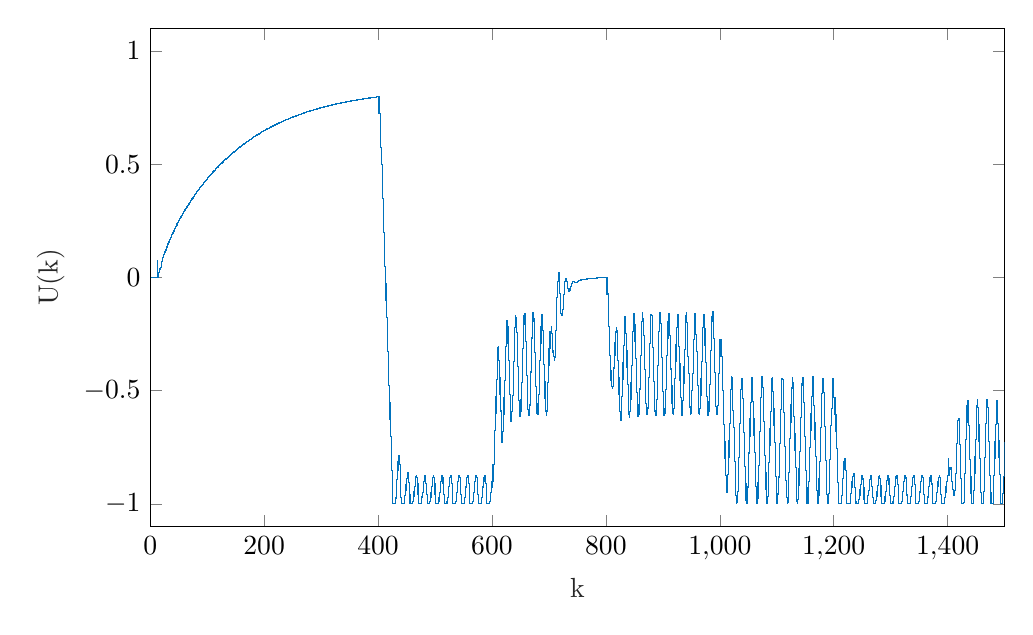
\begin{tikzpicture}

\begin{axis}[%
width=4.272in,
height=2.491in,
at={(0.717in,0.423in)},
scale only axis,
xmin=0,
xmax=1500,
xlabel style={font=\color{white!15!black}},
xlabel={k},
ymin=-1.1,
ymax=1.1,
ylabel style={font=\color{white!15!black}},
ylabel={U(k)},
axis background/.style={fill=white}
]
\addplot[const plot, color=mycolor1, forget plot] table[row sep=crcr] {%
1	0\\
2	0\\
3	0\\
4	0\\
5	0\\
6	0\\
7	0\\
8	0\\
9	0\\
10	0\\
11	0\\
12	0.075\\
13	0\\
14	0.0114285714285714\\
15	0.0228571428571429\\
16	0.0342857142857143\\
17	0.0365175839390572\\
18	0.0440148814813602\\
19	0.0595446953069174\\
20	0.0705851659663733\\
21	0.0789326719939548\\
22	0.086870350710181\\
23	0.0949549147436669\\
24	0.101845941231013\\
25	0.107854653767023\\
26	0.114077263247041\\
27	0.120628465205211\\
28	0.127258826854955\\
29	0.133863824227399\\
30	0.140481715930323\\
31	0.147043930161573\\
32	0.153434535182717\\
33	0.15962360940842\\
34	0.16564049829415\\
35	0.171515785285851\\
36	0.177268239604157\\
37	0.182918322234061\\
38	0.188485394736747\\
39	0.193978690425974\\
40	0.199399053723418\\
41	0.204745167310521\\
42	0.210016556942591\\
43	0.215213464644738\\
44	0.220336878449324\\
45	0.225388906354326\\
46	0.230372490131203\\
47	0.235290727657977\\
48	0.240146440733371\\
49	0.244942097655708\\
50	0.249679845363877\\
51	0.254361546283325\\
52	0.258988847140524\\
53	0.263563265543836\\
54	0.268086249955867\\
55	0.272559200387714\\
56	0.276983468931255\\
57	0.281360355781409\\
58	0.285691104247473\\
59	0.289976896306998\\
60	0.294218851241342\\
61	0.298418028026143\\
62	0.302575429796059\\
63	0.306692008622954\\
64	0.310768669886217\\
65	0.314806276060561\\
66	0.318805649855126\\
67	0.32276757675719\\
68	0.326692807172115\\
69	0.330582058353724\\
70	0.334436016227417\\
71	0.338255337137596\\
72	0.342040649524937\\
73	0.345792555529171\\
74	0.34951163250671\\
75	0.353198434453966\\
76	0.356853493334872\\
77	0.36047732031759\\
78	0.364070406927827\\
79	0.367633226126414\\
80	0.37116623331821\\
81	0.374669867298516\\
82	0.378144551142005\\
83	0.381590693038206\\
84	0.385008687077021\\
85	0.388398913987383\\
86	0.391761741832022\\
87	0.395097526661095\\
88	0.398406613127327\\
89	0.401689335065152\\
90	0.404946016036188\\
91	0.408176969843216\\
92	0.411382501014673\\
93	0.414562905261519\\
94	0.417718469908199\\
95	0.420849474299314\\
96	0.423956190183474\\
97	0.427038882075743\\
98	0.430097807599954\\
99	0.433133217812123\\
100	0.436145357506076\\
101	0.439134465502359\\
102	0.442100774921416\\
103	0.445044513441962\\
104	0.447965903545407\\
105	0.450865162747156\\
106	0.453742503815531\\
107	0.456598134979039\\
108	0.459432260122634\\
109	0.462245078973624\\
110	0.465036787277791\\
111	0.467807576966279\\
112	0.470557636313779\\
113	0.473287150088483\\
114	0.475996299694272\\
115	0.478685263305577\\
116	0.481354215995294\\
117	0.484003329856164\\
118	0.48663277411595\\
119	0.48924271524677\\
120	0.491833317068891\\
121	0.49440474084929\\
122	0.496957145395256\\
123	0.499490687143321\\
124	0.502005520243744\\
125	0.504501796640803\\
126	0.506979666149118\\
127	0.509439276526208\\
128	0.511880773541486\\
129	0.514304301041886\\
130	0.51671000101429\\
131	0.519098013644929\\
132	0.521468477375921\\
133	0.52382152895908\\
134	0.526157303507163\\
135	0.528475934542667\\
136	0.530777554044309\\
137	0.533062292491326\\
138	0.535330278905678\\
139	0.537581640892287\\
140	0.539816504677405\\
141	0.542034995145206\\
142	0.544237235872693\\
143	0.546423349163009\\
144	0.548593456077235\\
145	0.550747676464749\\
146	0.552886128992219\\
147	0.555008931171305\\
148	0.557116199385126\\
149	0.559208048913569\\
150	0.561284593957483\\
151	0.563345947661828\\
152	0.565392222137822\\
153	0.567423528484138\\
154	0.569439976807211\\
155	0.571441676240681\\
156	0.573428734964026\\
157	0.575401260220427\\
158	0.577359358333902\\
159	0.579303134725738\\
160	0.581232693930265\\
161	0.583148139610007\\
162	0.585049574570232\\
163	0.58693710077293\\
164	0.588810819350264\\
165	0.590670830617497\\
166	0.592517234085443\\
167	0.594350128472444\\
168	0.596169611715916\\
169	0.597975780983475\\
170	0.599768732683661\\
171	0.601548562476287\\
172	0.603315365282429\\
173	0.605069235294073\\
174	0.606810265983437\\
175	0.608538550111979\\
176	0.610254179739119\\
177	0.611957246230673\\
178	0.613647840267024\\
179	0.615326051851037\\
180	0.616991970315738\\
181	0.61864568433175\\
182	0.620287281914527\\
183	0.621916850431366\\
184	0.623534476608224\\
185	0.62514024653635\\
186	0.626734245678731\\
187	0.628316558876368\\
188	0.62988727035439\\
189	0.631446463728007\\
190	0.632994222008322\\
191	0.634530627607993\\
192	0.636055762346762\\
193	0.637569707456859\\
194	0.639072543588275\\
195	0.640564350813926\\
196	0.642045208634697\\
197	0.64351519598438\\
198	0.644974391234515\\
199	0.646422872199128\\
200	0.647860716139375\\
201	0.649287999768097\\
202	0.650704799254293\\
203	0.652111190227507\\
204	0.653507247782136\\
205	0.654893046481667\\
206	0.656268660362837\\
207	0.65763416293973\\
208	0.6589896272078\\
209	0.66033512564784\\
210	0.661670730229882\\
211	0.662996512417043\\
212	0.664312543169314\\
213	0.665618892947295\\
214	0.666915631715878\\
215	0.668202828947881\\
216	0.669480553627635\\
217	0.67074887425452\\
218	0.672007858846464\\
219	0.673257574943394\\
220	0.674498089610647\\
221	0.675729469442339\\
222	0.676951780564703\\
223	0.678165088639383\\
224	0.67936945886669\\
225	0.680564955988834\\
226	0.68175164429311\\
227	0.68292958761506\\
228	0.6840988493416\\
229	0.68525949241412\\
230	0.686411579331545\\
231	0.68755517215338\\
232	0.68869033250272\\
233	0.689817121569231\\
234	0.690935600112108\\
235	0.69204582846301\\
236	0.693147866528962\\
237	0.694241773795239\\
238	0.695327609328228\\
239	0.696405431778255\\
240	0.697475299382404\\
241	0.698537269967306\\
242	0.699591400951907\\
243	0.700637749350213\\
244	0.70167637177402\\
245	0.702707324435621\\
246	0.703730663150487\\
247	0.704746443339938\\
248	0.70575472003379\\
249	0.706755547872983\\
250	0.707748981112191\\
251	0.708735073622413\\
252	0.709713878893548\\
253	0.710685450036954\\
254	0.711649839787981\\
255	0.712607100508498\\
256	0.713557284189395\\
257	0.714500442453073\\
258	0.715436626555916\\
259	0.716365887390745\\
260	0.71728827548926\\
261	0.718203841024464\\
262	0.719112633813068\\
263	0.720014703317889\\
264	0.720910098650224\\
265	0.721798868572214\\
266	0.722681061499192\\
267	0.723556725502016\\
268	0.724425908309386\\
269	0.725288657310151\\
270	0.726145019555594\\
271	0.72699504176171\\
272	0.727838770311468\\
273	0.728676251257056\\
274	0.729507530322115\\
275	0.73033265290396\\
276	0.731151664075783\\
277	0.731964608588847\\
278	0.732771530874667\\
279	0.73357247504717\\
280	0.734367484904853\\
281	0.735156603932918\\
282	0.735939875305399\\
283	0.736717341887279\\
284	0.737489046236582\\
285	0.738255030606468\\
286	0.739015336947303\\
287	0.739770006908722\\
288	0.740519081841679\\
289	0.741262602800482\\
290	0.74200061054482\\
291	0.742733145541772\\
292	0.743460247967806\\
293	0.744181957710771\\
294	0.744898314371866\\
295	0.745609357267608\\
296	0.74631512543178\\
297	0.747015657617371\\
298	0.747710992298503\\
299	0.748401167672346\\
300	0.749086221661021\\
301	0.749766191913493\\
302	0.750441115807448\\
303	0.751111030451167\\
304	0.751775972685374\\
305	0.752435979085091\\
306	0.753091085961465\\
307	0.753741329363592\\
308	0.754386745080329\\
309	0.755027368642094\\
310	0.755663235322654\\
311	0.756294380140902\\
312	0.756920837862622\\
313	0.757542643002249\\
314	0.758159829824609\\
315	0.758772432346651\\
316	0.759380484339174\\
317	0.759984019328535\\
318	0.760583070598353\\
319	0.761177671191193\\
320	0.761767853910252\\
321	0.762353651321024\\
322	0.762935095752959\\
323	0.763512219301108\\
324	0.764085053827767\\
325	0.764653630964093\\
326	0.76521798211173\\
327	0.76577813844441\\
328	0.76633413090955\\
329	0.766885990229836\\
330	0.767433746904798\\
331	0.767977431212379\\
332	0.768517073210486\\
333	0.769052702738536\\
334	0.76958434941899\\
335	0.770112042658881\\
336	0.770635811651328\\
337	0.771155685377038\\
338	0.771671692605807\\
339	0.772183861898003\\
340	0.772692221606043\\
341	0.773196799875856\\
342	0.773697624648348\\
343	0.774194723660841\\
344	0.774688124448517\\
345	0.775177854345843\\
346	0.775663940487994\\
347	0.776146409812256\\
348	0.776625289059437\\
349	0.777100604775249\\
350	0.777572383311693\\
351	0.778040650828438\\
352	0.778505433294174\\
353	0.778966756487977\\
354	0.779424646000651\\
355	0.779879127236064\\
356	0.780330225412477\\
357	0.780777965563867\\
358	0.78122237254123\\
359	0.781663471013892\\
360	0.782101285470795\\
361	0.782535840221785\\
362	0.782967159398886\\
363	0.783395266957569\\
364	0.783820186678013\\
365	0.78424194216635\\
366	0.784660556855911\\
367	0.785076054008459\\
368	0.785488456715414\\
369	0.785897787899072\\
370	0.786304070313809\\
371	0.786707326547289\\
372	0.78710757902165\\
373	0.787504849994694\\
374	0.787899161561059\\
375	0.78829053565339\\
376	0.788678994043502\\
377	0.789064558343527\\
378	0.789447250007063\\
379	0.789827090330312\\
380	0.790204100453207\\
381	0.790578301360535\\
382	0.790949713883048\\
383	0.791318358698577\\
384	0.791684256333123\\
385	0.792047427161952\\
386	0.792407891410678\\
387	0.792765669156342\\
388	0.793120780328476\\
389	0.793473244710172\\
390	0.793823081939129\\
391	0.794170311508705\\
392	0.794514952768956\\
393	0.794857024927667\\
394	0.795196547051382\\
395	0.795533538066417\\
396	0.795868016759878\\
397	0.79620000178066\\
398	0.796529511640448\\
399	0.796856564714707\\
400	0.797181179243666\\
401	0.722181179243666\\
402	0.797181179243666\\
403	0.722181179243666\\
404	0.647181179243666\\
405	0.572181179243666\\
406	0.497181179243666\\
407	0.422181179243666\\
408	0.347181179243666\\
409	0.272181179243666\\
410	0.197181179243666\\
411	0.122181179243666\\
412	0.0471811792436657\\
413	-0.0278188207563343\\
414	-0.102818820756334\\
415	-0.177818820756334\\
416	-0.252818820756334\\
417	-0.327818820756334\\
418	-0.402818820756334\\
419	-0.477818820756334\\
420	-0.552818820756334\\
421	-0.627818820756334\\
422	-0.702818820756334\\
423	-0.777818820756334\\
424	-0.852818820756334\\
425	-0.927818820756334\\
426	-1\\
427	-1\\
428	-1\\
429	-1\\
430	-1\\
431	-0.974640609872317\\
432	-0.934447651620375\\
433	-0.893228816843996\\
434	-0.852413069833593\\
435	-0.812913849113112\\
436	-0.787490817809094\\
437	-0.789987508928565\\
438	-0.825939745640636\\
439	-0.89690680724809\\
440	-0.97190680724809\\
441	-1\\
442	-1\\
443	-1\\
444	-1\\
445	-1\\
446	-0.986942739511209\\
447	-0.965258778450122\\
448	-0.940986927614609\\
449	-0.915229903118682\\
450	-0.888784513865481\\
451	-0.868738667269224\\
452	-0.862736985501717\\
453	-0.87478106217527\\
454	-0.907024130497581\\
455	-0.960651750941539\\
456	-1\\
457	-1\\
458	-1\\
459	-1\\
460	-1\\
461	-0.989506725093926\\
462	-0.96937699391941\\
463	-0.947112511565755\\
464	-0.923556334101131\\
465	-0.899325638571134\\
466	-0.880179993253913\\
467	-0.873658469178974\\
468	-0.883539333273103\\
469	-0.911672568041885\\
470	-0.959130859926508\\
471	-1\\
472	-1\\
473	-1\\
474	-1\\
475	-1\\
476	-0.989976583083068\\
477	-0.970180633090911\\
478	-0.948305073800128\\
479	-0.925153961466417\\
480	-0.901318154239029\\
481	-0.882313058905409\\
482	-0.875638194584942\\
483	-0.885039107831719\\
484	-0.912328789732188\\
485	-0.95857348911926\\
486	-1\\
487	-1\\
488	-1\\
489	-1\\
490	-1\\
491	-0.990115256018187\\
492	-0.970384079376209\\
493	-0.948580738604675\\
494	-0.925503015815491\\
495	-0.901737608037295\\
496	-0.882728478807282\\
497	-0.875982192650075\\
498	-0.885248599827726\\
499	-0.912336332159386\\
500	-0.95831232839988\\
501	-1\\
502	-1\\
503	-1\\
504	-1\\
505	-1\\
506	-0.990175607663222\\
507	-0.970462306573185\\
508	-0.948675837039504\\
509	-0.925613465651995\\
510	-0.901861630234328\\
511	-0.882833604986016\\
512	-0.876044848042896\\
513	-0.885252380098009\\
514	-0.912265943566088\\
515	-0.95815420717522\\
516	-1\\
517	-1\\
518	-1\\
519	-1\\
520	-1\\
521	-0.990210648837345\\
522	-0.970504773957689\\
523	-0.948724056002422\\
524	-0.925666047218092\\
525	-0.9019174432304\\
526	-0.882873805956469\\
527	-0.87605741040862\\
528	-0.885230872469213\\
529	-0.912205358071569\\
530	-0.958050897435366\\
531	-1\\
532	-1\\
533	-1\\
534	-1\\
535	-1\\
536	-0.990233271949823\\
537	-0.970531604220884\\
538	-0.948753788129586\\
539	-0.925697679490606\\
540	-0.901950223622715\\
541	-0.882895569690177\\
542	-0.87606072265761\\
543	-0.88521220019881\\
544	-0.912162246721167\\
545	-0.957981845358946\\
546	-1\\
547	-1\\
548	-1\\
549	-1\\
550	-1\\
551	-0.99024834341582\\
552	-0.970549371198093\\
553	-0.948773340495677\\
554	-0.925718330965849\\
555	-0.901971469364639\\
556	-0.88290930600189\\
557	-0.876062056776985\\
558	-0.885198891295794\\
559	-0.912132801273502\\
560	-0.957935417989174\\
561	-1\\
562	-1\\
563	-1\\
564	-1\\
565	-1\\
566	-0.990258468134496\\
567	-0.970561287866676\\
568	-0.948786430547658\\
569	-0.925732130019774\\
570	-0.90198563758836\\
571	-0.882918399651323\\
572	-0.876062799590646\\
573	-0.88518979777437\\
574	-0.912112893022965\\
575	-0.95790415437327\\
576	-1\\
577	-1\\
578	-1\\
579	-1\\
580	-1\\
581	-0.990265284506695\\
582	-0.970569307369419\\
583	-0.948795235481924\\
584	-0.925741407157017\\
585	-0.901995158017671\\
586	-0.882924498490891\\
587	-0.876063272981528\\
588	-0.885183649079702\\
589	-0.912099467892759\\
590	-0.957883093580869\\
591	-1\\
592	-1\\
593	-1\\
594	-1\\
595	-1\\
596	-0.990269876119297\\
597	-0.970574708861882\\
598	-0.94880116526507\\
599	-0.925747654131358\\
600	-0.902001567963008\\
601	-0.827001567963008\\
602	-0.902001567963008\\
603	-0.827001567963008\\
604	-0.752001567963008\\
605	-0.677001567963008\\
606	-0.602001567963008\\
607	-0.527001567963008\\
608	-0.452001567963008\\
609	-0.377001567963008\\
610	-0.310290888034597\\
611	-0.307119617857521\\
612	-0.365476715476994\\
613	-0.440476715476994\\
614	-0.515476715476994\\
615	-0.590476715476994\\
616	-0.665476715476994\\
617	-0.729511671602751\\
618	-0.730118425776315\\
619	-0.681162640498566\\
620	-0.606162640498566\\
621	-0.531162640498566\\
622	-0.456162640498566\\
623	-0.381162640498566\\
624	-0.306162640498566\\
625	-0.231162640498566\\
626	-0.192848082184194\\
627	-0.218429195104676\\
628	-0.293429195104676\\
629	-0.368429195104676\\
630	-0.443429195104676\\
631	-0.518429195104676\\
632	-0.593429195104676\\
633	-0.635950142264871\\
634	-0.633276809888131\\
635	-0.594434685720071\\
636	-0.522440244685862\\
637	-0.447440244685862\\
638	-0.372440244685862\\
639	-0.297440244685862\\
640	-0.222440244685862\\
641	-0.168615259739676\\
642	-0.176369904759094\\
643	-0.245412655433871\\
644	-0.320412655433871\\
645	-0.395412655433871\\
646	-0.470412655433872\\
647	-0.545412655433872\\
648	-0.602617238550442\\
649	-0.615260891051632\\
650	-0.592839964390872\\
651	-0.538793468313336\\
652	-0.463793468313336\\
653	-0.388793468313336\\
654	-0.313793468313336\\
655	-0.238793468313336\\
656	-0.170207468777193\\
657	-0.158680867933574\\
658	-0.208901891705192\\
659	-0.283901891705192\\
660	-0.358901891705192\\
661	-0.433901891705192\\
662	-0.508901891705192\\
663	-0.583901891705192\\
664	-0.612134192049751\\
665	-0.603735143500423\\
666	-0.563748989291815\\
667	-0.493122038996966\\
668	-0.418122038996966\\
669	-0.343122038996966\\
670	-0.268122038996966\\
671	-0.193122038996966\\
672	-0.15749355289828\\
673	-0.183110444971742\\
674	-0.258110444971742\\
675	-0.333110444971742\\
676	-0.408110444971742\\
677	-0.483110444971742\\
678	-0.558110444971742\\
679	-0.602361474653915\\
680	-0.606104015102179\\
681	-0.576960318623457\\
682	-0.517023029221991\\
683	-0.442023029221991\\
684	-0.367023029221991\\
685	-0.292023029221991\\
686	-0.217023029221991\\
687	-0.163165930719003\\
688	-0.16801802822614\\
689	-0.233715275033753\\
690	-0.308715275033753\\
691	-0.383715275033753\\
692	-0.458715275033753\\
693	-0.533715275033753\\
694	-0.593236218425478\\
695	-0.609113344811441\\
696	-0.59041434543564\\
697	-0.540566527997188\\
698	-0.465566527997188\\
699	-0.390566527997187\\
700	-0.315566527997187\\
701	-0.240566527997187\\
702	-0.315566527997187\\
703	-0.240566527997187\\
704	-0.216268068722606\\
705	-0.248425638235088\\
706	-0.323293320322464\\
707	-0.332161329577871\\
708	-0.349804944862051\\
709	-0.367391844164065\\
710	-0.355707473266625\\
711	-0.303289783568077\\
712	-0.235896254270488\\
713	-0.1637557139973\\
714	-0.0887557139972998\\
715	-0.0193289520909364\\
716	0.0202434416159918\\
717	0.0192073874154682\\
718	-0.0171045838529739\\
719	-0.0730741091384629\\
720	-0.126757081647338\\
721	-0.159509759178614\\
722	-0.169334099170884\\
723	-0.162478510344448\\
724	-0.14288591965973\\
725	-0.112641353259688\\
726	-0.0769984940265784\\
727	-0.0438684478973392\\
728	-0.0195310954148731\\
729	-0.00734998507554641\\
730	-0.00814093636898694\\
731	-0.0192816832457184\\
732	-0.0348649240510183\\
733	-0.0488019936933403\\
734	-0.0575920089594108\\
735	-0.060408695180101\\
736	-0.0578746852649811\\
737	-0.051274353599664\\
738	-0.0423791449977399\\
739	-0.0331861929137714\\
740	-0.0254146188879418\\
741	-0.0201315575598368\\
742	-0.017649964675223\\
743	-0.0175897670795725\\
744	-0.0190751869302565\\
745	-0.0210674511927056\\
746	-0.0226946603947036\\
747	-0.0234293774839162\\
748	-0.0231038978229855\\
749	-0.0218385923798186\\
750	-0.0199396448768455\\
751	-0.0177879369093164\\
752	-0.0157368893802598\\
753	-0.0140396549159317\\
754	-0.0128160802655215\\
755	-0.0120572094953171\\
756	-0.0116582483460677\\
757	-0.0114667734090296\\
758	-0.0113306794093521\\
759	-0.0111332617745134\\
760	-0.0108100915419304\\
761	-0.0103491000115152\\
762	-0.00977882817623969\\
763	-0.00915075815730428\\
764	-0.00852122544718229\\
765	-0.00793706501758778\\
766	-0.00742722818667896\\
767	-0.00700069020891932\\
768	-0.00664948883638402\\
769	-0.00635486477298208\\
770	-0.00609426019297272\\
771	-0.00584730812820822\\
772	-0.00559969187461339\\
773	-0.00534456880944111\\
774	-0.00508190432058059\\
775	-0.00481644421821981\\
776	-0.00455516269047657\\
777	-0.00430491136210078\\
778	-0.00407074954921444\\
779	-0.00385514921865837\\
780	-0.00365801621805339\\
781	-0.0034772988572156\\
782	-0.00330988269900292\\
783	-0.00315248717819132\\
784	-0.00300235769669363\\
785	-0.0028576510486263\\
786	-0.00271751079450642\\
787	-0.00258190120536167\\
788	-0.00245130458075454\\
789	-0.0023263888349335\\
790	-0.0022077293008691\\
791	-0.00209563296796552\\
792	-0.0019900765675462\\
793	-0.00189074074050602\\
794	-0.00179710551384117\\
795	-0.00170856799509218\\
796	-0.00162454903008699\\
797	-0.00154456739092348\\
798	-0.00146827348455609\\
799	-0.00139544607303339\\
800	-0.00132596297876445\\
801	-0.0763259629787644\\
802	-0.00132596297876444\\
803	-0.0726947325161335\\
804	-0.14406657753129\\
805	-0.215441368811505\\
806	-0.275901887866343\\
807	-0.34401196410316\\
808	-0.409890322684653\\
809	-0.455549056300939\\
810	-0.482227445456514\\
811	-0.491798396810679\\
812	-0.481777150346817\\
813	-0.449552089284939\\
814	-0.400508693352417\\
815	-0.343364743140259\\
816	-0.2868744326723\\
817	-0.241521375407176\\
818	-0.22057006588254\\
819	-0.235773041339282\\
820	-0.291886083319734\\
821	-0.366886083319734\\
822	-0.441886083319734\\
823	-0.516886083319734\\
824	-0.591886083319734\\
825	-0.630487519520783\\
826	-0.630020368362443\\
827	-0.594095728291711\\
828	-0.524901808619869\\
829	-0.449901808619869\\
830	-0.374901808619869\\
831	-0.299901808619869\\
832	-0.224901808619869\\
833	-0.171369841351282\\
834	-0.178711786083006\\
835	-0.247163523419689\\
836	-0.322163523419689\\
837	-0.397163523419689\\
838	-0.472163523419689\\
839	-0.547163523419689\\
840	-0.604432003117832\\
841	-0.616924496529591\\
842	-0.594135480346229\\
843	-0.539568904178249\\
844	-0.464568904178249\\
845	-0.389568904178249\\
846	-0.314568904178249\\
847	-0.239568904178249\\
848	-0.17066916819033\\
849	-0.158943843894124\\
850	-0.209003155685519\\
851	-0.284003155685519\\
852	-0.359003155685519\\
853	-0.434003155685519\\
854	-0.509003155685519\\
855	-0.584003155685519\\
856	-0.612344007971038\\
857	-0.603976310124707\\
858	-0.563982603843234\\
859	-0.493328014091446\\
860	-0.418328014091446\\
861	-0.343328014091446\\
862	-0.268328014091446\\
863	-0.193328014091446\\
864	-0.157569673199754\\
865	-0.183064836035515\\
866	-0.258064836035515\\
867	-0.333064836035515\\
868	-0.408064836035515\\
869	-0.483064836035515\\
870	-0.558064836035515\\
871	-0.602389334688621\\
872	-0.606175606795592\\
873	-0.5770619584669\\
874	-0.517148787895559\\
875	-0.442148787895559\\
876	-0.367148787895559\\
877	-0.292148787895559\\
878	-0.217148787895559\\
879	-0.163207859966071\\
880	-0.167969652998936\\
881	-0.23358319841291\\
882	-0.30858319841291\\
883	-0.38358319841291\\
884	-0.458583198412911\\
885	-0.53358319841291\\
886	-0.593187289847158\\
887	-0.609131828930848\\
888	-0.590489373174063\\
889	-0.540695546321064\\
890	-0.465695546321064\\
891	-0.390695546321064\\
892	-0.315695546321064\\
893	-0.240695546321063\\
894	-0.170010505615207\\
895	-0.155318173683562\\
896	-0.202347064574727\\
897	-0.277347064574727\\
898	-0.352347064574727\\
899	-0.427347064574727\\
900	-0.502347064574727\\
901	-0.577347064574727\\
902	-0.608126533931625\\
903	-0.602065209001814\\
904	-0.564473309480019\\
905	-0.496394583427273\\
906	-0.421394583427273\\
907	-0.346394583427273\\
908	-0.271394583427273\\
909	-0.196394583427273\\
910	-0.157834833303133\\
911	-0.179936669487806\\
912	-0.254936669487806\\
913	-0.329936669487806\\
914	-0.404936669487806\\
915	-0.479936669487806\\
916	-0.554936669487806\\
917	-0.60122412812095\\
918	-0.606493604922362\\
919	-0.578698689217864\\
920	-0.520080869321503\\
921	-0.445080869321503\\
922	-0.370080869321503\\
923	-0.295080869321503\\
924	-0.220080869321503\\
925	-0.164004027107253\\
926	-0.166300300393891\\
927	-0.229587197673581\\
928	-0.304587197673581\\
929	-0.379587197673581\\
930	-0.454587197673581\\
931	-0.529587197673581\\
932	-0.591448488330577\\
933	-0.609286127951084\\
934	-0.592280781655214\\
935	-0.544083206579714\\
936	-0.469083206579714\\
937	-0.394083206579714\\
938	-0.319083206579714\\
939	-0.244083206579714\\
940	-0.171021297742325\\
941	-0.153506711194384\\
942	-0.197791888928116\\
943	-0.272791888928116\\
944	-0.347791888928116\\
945	-0.422791888928116\\
946	-0.497791888928116\\
947	-0.572791888928116\\
948	-0.605709670332124\\
949	-0.601424561661385\\
950	-0.565550381513044\\
951	-0.499253505468422\\
952	-0.424253505468422\\
953	-0.349253505468422\\
954	-0.274253505468422\\
955	-0.199253505468422\\
956	-0.1582823025779\\
957	-0.177561615462287\\
958	-0.252561615462287\\
959	-0.327561615462287\\
960	-0.402561615462287\\
961	-0.477561615462287\\
962	-0.552561615462287\\
963	-0.600494832529512\\
964	-0.606962537520918\\
965	-0.580200993137346\\
966	-0.522579768974096\\
967	-0.447579768974096\\
968	-0.372579768974096\\
969	-0.297579768974096\\
970	-0.222579768974096\\
971	-0.164719697830541\\
972	-0.164974346386\\
973	-0.226332670558384\\
974	-0.301332670558384\\
975	-0.376332670558384\\
976	-0.451332670558384\\
977	-0.526332670558384\\
978	-0.590081011816656\\
979	-0.609477630879612\\
980	-0.593807474290508\\
981	-0.546906033174981\\
982	-0.471906033174981\\
983	-0.396906033174981\\
984	-0.321906033174981\\
985	-0.246906033174981\\
986	-0.171906033174981\\
987	-0.152064716644883\\
988	-0.19408175443561\\
989	-0.26908175443561\\
990	-0.34408175443561\\
991	-0.41908175443561\\
992	-0.49408175443561\\
993	-0.56908175443561\\
994	-0.603751821756061\\
995	-0.600909347409391\\
996	-0.566425680453061\\
997	-0.501570882936241\\
998	-0.426570882936241\\
999	-0.351570882936241\\
1000	-0.276570882936241\\
1001	-0.351570882936241\\
1002	-0.276570882936241\\
1003	-0.351570882936241\\
1004	-0.426570882936241\\
1005	-0.501570882936241\\
1006	-0.576570882936241\\
1007	-0.651570882936241\\
1008	-0.726570882936241\\
1009	-0.801570882936241\\
1010	-0.876570882936241\\
1011	-0.930936686428785\\
1012	-0.94862867249531\\
1013	-0.929232332971211\\
1014	-0.871589303257687\\
1015	-0.796589303257687\\
1016	-0.721589303257687\\
1017	-0.646589303257687\\
1018	-0.571589303257687\\
1019	-0.496589303257687\\
1020	-0.43826714064203\\
1021	-0.442805699136262\\
1022	-0.514356764752773\\
1023	-0.589356764752773\\
1024	-0.664356764752773\\
1025	-0.739356764752773\\
1026	-0.814356764752773\\
1027	-0.889356764752773\\
1028	-0.964356764752773\\
1029	-1\\
1030	-0.995736426742797\\
1031	-0.946175530981625\\
1032	-0.871175530981625\\
1033	-0.796175530981625\\
1034	-0.721175530981625\\
1035	-0.646175530981625\\
1036	-0.571175530981625\\
1037	-0.496175530981625\\
1038	-0.445402928694153\\
1039	-0.459211216887546\\
1040	-0.534211216887546\\
1041	-0.609211216887546\\
1042	-0.684211216887546\\
1043	-0.759211216887546\\
1044	-0.834211216887546\\
1045	-0.909211216887546\\
1046	-0.984211216887546\\
1047	-1\\
1048	-0.985720572469908\\
1049	-0.925834475023711\\
1050	-0.850834475023711\\
1051	-0.775834475023711\\
1052	-0.700834475023711\\
1053	-0.625834475023711\\
1054	-0.550834475023711\\
1055	-0.475834475023711\\
1056	-0.442126360475719\\
1057	-0.474014170164811\\
1058	-0.549014170164811\\
1059	-0.624014170164811\\
1060	-0.699014170164811\\
1061	-0.774014170164811\\
1062	-0.849014170164811\\
1063	-0.924014170164811\\
1064	-0.998985659149325\\
1065	-1\\
1066	-0.976184424346918\\
1067	-0.907132764492283\\
1068	-0.832132764492283\\
1069	-0.757132764492283\\
1070	-0.682132764492283\\
1071	-0.607132764492283\\
1072	-0.532132764492284\\
1073	-0.457132764492284\\
1074	-0.439160177066725\\
1075	-0.487691827022259\\
1076	-0.562691827022259\\
1077	-0.637691827022259\\
1078	-0.712691827022259\\
1079	-0.787691827022259\\
1080	-0.862691827022259\\
1081	-0.937691827022259\\
1082	-1\\
1083	-1\\
1084	-0.967387249064964\\
1085	-0.892387249064964\\
1086	-0.817387249064964\\
1087	-0.742387249064964\\
1088	-0.667387249064964\\
1089	-0.592387249064964\\
1090	-0.517387249064964\\
1091	-0.448933242533163\\
1092	-0.443571103662323\\
1093	-0.505330799805562\\
1094	-0.580330799805562\\
1095	-0.655330799805562\\
1096	-0.730330799805562\\
1097	-0.805330799805562\\
1098	-0.880330799805562\\
1099	-0.955330799805562\\
1100	-1\\
1101	-1\\
1102	-0.956938087871941\\
1103	-0.881938087871941\\
1104	-0.806938087871941\\
1105	-0.731938087871941\\
1106	-0.656938087871941\\
1107	-0.581938087871941\\
1108	-0.506938087871941\\
1109	-0.447411905257931\\
1110	-0.451789891913006\\
1111	-0.523700475407019\\
1112	-0.598700475407019\\
1113	-0.673700475407019\\
1114	-0.748700475407019\\
1115	-0.823700475407019\\
1116	-0.898700475407018\\
1117	-0.973700475407018\\
1118	-1\\
1119	-0.992230717743547\\
1120	-0.938646743057404\\
1121	-0.863646743057404\\
1122	-0.788646743057404\\
1123	-0.713646743057404\\
1124	-0.638646743057405\\
1125	-0.563646743057405\\
1126	-0.488646743057405\\
1127	-0.44430425089889\\
1128	-0.464902697806308\\
1129	-0.539902697806309\\
1130	-0.614902697806308\\
1131	-0.689902697806308\\
1132	-0.764902697806308\\
1133	-0.839902697806308\\
1134	-0.914902697806308\\
1135	-0.989902697806308\\
1136	-1\\
1137	-0.982075477702107\\
1138	-0.918685268845865\\
1139	-0.843685268845865\\
1140	-0.768685268845865\\
1141	-0.693685268845865\\
1142	-0.618685268845865\\
1143	-0.543685268845865\\
1144	-0.468685268845865\\
1145	-0.440959593657043\\
1146	-0.479184610499197\\
1147	-0.554184610499197\\
1148	-0.629184610499197\\
1149	-0.704184610499197\\
1150	-0.779184610499197\\
1151	-0.854184610499197\\
1152	-0.929184610499197\\
1153	-1\\
1154	-1\\
1155	-0.972851906699943\\
1156	-0.900587977104589\\
1157	-0.825587977104589\\
1158	-0.750587977104589\\
1159	-0.675587977104589\\
1160	-0.600587977104589\\
1161	-0.525587977104589\\
1162	-0.450654379684978\\
1163	-0.438205640828532\\
1164	-0.492539287463969\\
1165	-0.567539287463969\\
1166	-0.642539287463969\\
1167	-0.717539287463969\\
1168	-0.792539287463969\\
1169	-0.867539287463969\\
1170	-0.942539287463969\\
1171	-1\\
1172	-1\\
1173	-0.964273879569429\\
1174	-0.889273879569429\\
1175	-0.814273879569429\\
1176	-0.739273879569429\\
1177	-0.664273879569429\\
1178	-0.589273879569429\\
1179	-0.514273879569429\\
1180	-0.448386588350385\\
1181	-0.445838539453476\\
1182	-0.510545857125852\\
1183	-0.585545857125852\\
1184	-0.660545857125852\\
1185	-0.735545857125852\\
1186	-0.810545857125852\\
1187	-0.885545857125852\\
1188	-0.960545857125852\\
1189	-1\\
1190	-0.999909970095917\\
1191	-0.953861639387507\\
1192	-0.878861639387507\\
1193	-0.803861639387507\\
1194	-0.728861639387507\\
1195	-0.653861639387507\\
1196	-0.578861639387507\\
1197	-0.503861639387507\\
1198	-0.447016400369095\\
1199	-0.454304738138049\\
1200	-0.529233759756202\\
1201	-0.604233759756202\\
1202	-0.529233759756202\\
1203	-0.604233759756202\\
1204	-0.679233759756202\\
1205	-0.754233759756202\\
1206	-0.829233759756202\\
1207	-0.904233759756202\\
1208	-0.979233759756202\\
1209	-1\\
1210	-1\\
1211	-1\\
1212	-1\\
1213	-0.993981763268111\\
1214	-0.963128856890745\\
1215	-0.925809507099741\\
1216	-0.887338013868427\\
1217	-0.849046482581572\\
1218	-0.814613460465493\\
1219	-0.798139634660734\\
1220	-0.809401912077866\\
1221	-0.852136899172258\\
1222	-0.927136899172258\\
1223	-1\\
1224	-1\\
1225	-1\\
1226	-1\\
1227	-1\\
1228	-0.997037828494699\\
1229	-0.977408619645817\\
1230	-0.954575015225976\\
1231	-0.929779648906701\\
1232	-0.903935177369368\\
1233	-0.87915872362532\\
1234	-0.864992879702823\\
1235	-0.867141122971712\\
1236	-0.888247558659017\\
1237	-0.9299442177336\\
1238	-0.99213999038188\\
1239	-1\\
1240	-1\\
1241	-1\\
1242	-1\\
1243	-0.999962119225071\\
1244	-0.982561464990029\\
1245	-0.961260869664094\\
1246	-0.938298347044186\\
1247	-0.914388919053088\\
1248	-0.890067443026504\\
1249	-0.874585693317927\\
1250	-0.873946879598568\\
1251	-0.890655482676272\\
1252	-0.926175208360352\\
1253	-0.981244407203259\\
1254	-1\\
1255	-1\\
1256	-1\\
1257	-1\\
1258	-1\\
1259	-0.98517568789725\\
1260	-0.964555175596886\\
1261	-0.942153035943481\\
1262	-0.918697070618195\\
1263	-0.894716946300494\\
1264	-0.878161597081924\\
1265	-0.875478070007118\\
1266	-0.889551248855405\\
1267	-0.921947845192847\\
1268	-0.973523664092593\\
1269	-1\\
1270	-1\\
1271	-1\\
1272	-1\\
1273	-1\\
1274	-0.986860538276553\\
1275	-0.966559780515419\\
1276	-0.94438689502555\\
1277	-0.921089295227273\\
1278	-0.897213094907827\\
1279	-0.879849354306475\\
1280	-0.875799058459425\\
1281	-0.888232921685441\\
1282	-0.918794635241522\\
1283	-0.968409366691174\\
1284	-1\\
1285	-1\\
1286	-1\\
1287	-1\\
1288	-1\\
1289	-0.987976183043833\\
1290	-0.967876306517002\\
1291	-0.945838042796297\\
1292	-0.922624864208082\\
1293	-0.898795950611674\\
1294	-0.880876239438118\\
1295	-0.875906451137064\\
1296	-0.88725316121136\\
1297	-0.916615172899041\\
1298	-0.96496563625316\\
1299	-1\\
1300	-1\\
1301	-1\\
1302	-1\\
1303	-1\\
1304	-0.988726441327826\\
1305	-0.968759280443355\\
1306	-0.946808211748917\\
1307	-0.923648010876424\\
1308	-0.899846997272859\\
1309	-0.881550239946226\\
1310	-0.875960417979495\\
1311	-0.886576895683549\\
1312	-0.915136097814434\\
1313	-0.962643667741123\\
1314	-1\\
1315	-1\\
1316	-1\\
1317	-1\\
1318	-1\\
1319	-0.989232327624706\\
1320	-0.969354329471967\\
1321	-0.947461525372853\\
1322	-0.924336410459924\\
1323	-0.900553536274737\\
1324	-0.882002212067142\\
1325	-0.875994219327254\\
1326	-0.886118610687541\\
1327	-0.914137263825524\\
1328	-0.961077763892053\\
1329	-1\\
1330	-1\\
1331	-1\\
1332	-1\\
1333	-1\\
1334	-0.989573544045389\\
1335	-0.969755653241561\\
1336	-0.947902070441412\\
1337	-0.924800517254906\\
1338	-0.90102976294091\\
1339	-0.882306778671936\\
1340	-0.876016819895232\\
1341	-0.885809442466032\\
1342	-0.913463697041042\\
1343	-0.960021967127593\\
1344	-1\\
1345	-1\\
1346	-1\\
1347	-1\\
1348	-1\\
1349	-0.989803640789891\\
1350	-0.970026289560627\\
1351	-0.948199149151281\\
1352	-0.925113470369197\\
1353	-0.901350870184759\\
1354	-0.882512181620616\\
1355	-0.876032142353344\\
1356	-0.88560110194344\\
1357	-0.913009688265638\\
1358	-0.95931026089\\
1359	-1\\
1360	-1\\
1361	-1\\
1362	-1\\
1363	-1\\
1364	-0.989958765026542\\
1365	-0.970208751018571\\
1366	-0.948399439492436\\
1367	-0.92532446195867\\
1368	-0.901567356314583\\
1369	-0.882650693542068\\
1370	-0.87604253939253\\
1371	-0.885460740689487\\
1372	-0.912703727850892\\
1373	-0.958830584142223\\
1374	-1\\
1375	-1\\
1376	-1\\
1377	-1\\
1378	-1\\
1379	-0.99006332408823\\
1380	-0.97033173998023\\
1381	-0.948534447627047\\
1382	-0.925466683734721\\
1383	-0.90171328137557\\
1384	-0.882744076006269\\
1385	-0.87604958304373\\
1386	-0.885366181001938\\
1387	-0.912497558190686\\
1388	-0.958507328952657\\
1389	-1\\
1390	-1\\
1391	-1\\
1392	-1\\
1393	-1\\
1394	-0.990133790450501\\
1395	-0.970414628740323\\
1396	-0.948625437582644\\
1397	-0.92556253570025\\
1398	-0.901811629201744\\
1399	-0.882807020212707\\
1400	-0.876054347146135\\
1401	-0.801054347146135\\
1402	-0.876054347146135\\
1403	-0.850556640121169\\
1404	-0.841449481567065\\
1405	-0.840501128570021\\
1406	-0.886243389233104\\
1407	-0.900841423887538\\
1408	-0.915809355799678\\
1409	-0.938896411367326\\
1410	-0.962819049214551\\
1411	-0.961108058710565\\
1412	-0.942216463431944\\
1413	-0.911368048472954\\
1414	-0.86483393065799\\
1415	-0.801046375361089\\
1416	-0.732331600964303\\
1417	-0.672388843671238\\
1418	-0.631864324531971\\
1419	-0.623307300437791\\
1420	-0.662094521521616\\
1421	-0.737094521521615\\
1422	-0.812094521521615\\
1423	-0.887094521521615\\
1424	-0.962094521521615\\
1425	-1\\
1426	-1\\
1427	-1\\
1428	-0.995372272052974\\
1429	-0.941333569641269\\
1430	-0.866333569641269\\
1431	-0.791333569641269\\
1432	-0.716333569641269\\
1433	-0.641333569641269\\
1434	-0.566370200462619\\
1435	-0.54299216484516\\
1436	-0.581007174286643\\
1437	-0.656007174286643\\
1438	-0.731007174286643\\
1439	-0.806007174286643\\
1440	-0.881007174286643\\
1441	-0.956007174286643\\
1442	-1\\
1443	-1\\
1444	-1\\
1445	-0.994439878863576\\
1446	-0.940808303525377\\
1447	-0.865808303525377\\
1448	-0.790808303525377\\
1449	-0.715808303525377\\
1450	-0.640808303525377\\
1451	-0.565808303525377\\
1452	-0.540406686775146\\
1453	-0.576509605322702\\
1454	-0.651509605322702\\
1455	-0.726509605322702\\
1456	-0.801509605322702\\
1457	-0.876509605322702\\
1458	-0.951509605322701\\
1459	-1\\
1460	-1\\
1461	-1\\
1462	-0.997001265589931\\
1463	-0.9459828309123\\
1464	-0.8709828309123\\
1465	-0.7959828309123\\
1466	-0.7209828309123\\
1467	-0.6459828309123\\
1468	-0.5709828309123\\
1469	-0.541525925009174\\
1470	-0.573240154773689\\
1471	-0.648240154773689\\
1472	-0.723240154773689\\
1473	-0.798240154773689\\
1474	-0.873240154773689\\
1475	-0.948240154773689\\
1476	-1\\
1477	-1\\
1478	-1\\
1479	-0.999250183278152\\
1480	-0.950407467488723\\
1481	-0.875407467488723\\
1482	-0.800407467488723\\
1483	-0.725407467488723\\
1484	-0.650407467488723\\
1485	-0.575407467488723\\
1486	-0.542597384979512\\
1487	-0.570657021434135\\
1488	-0.645657021434135\\
1489	-0.720657021434135\\
1490	-0.795657021434135\\
1491	-0.870657021434135\\
1492	-0.945657021434135\\
1493	-1\\
1494	-1\\
1495	-1\\
1496	-1\\
1497	-0.952891144338267\\
1498	-0.877891144338267\\
1499	-0.802891144338267\\
1500	-0.727891144338267\\
};
\end{axis}
\end{tikzpicture}%
\caption{Sterowanie, $K = 1; T_i=3,5; T_d=0,84;$}
\end{figure}

\begin{equation}
    E = \num{3,2788e7}
\end{equation}

Błąd się zmniejszył, więc kontynuujemy zmniejszanie $K$:

\begin{equation}
    K = 0,4
\end{equation}

\begin{figure}[H]
\centering
% This file was created by matlab2tikz.
%
%The latest updates can be retrieved from
%  http://www.mathworks.com/matlabcentral/fileexchange/22022-matlab2tikz-matlab2tikz
%where you can also make suggestions and rate matlab2tikz.
%
\definecolor{mycolor1}{rgb}{0.00000,0.44700,0.74100}%
\definecolor{mycolor2}{rgb}{0.85000,0.32500,0.09800}%
%
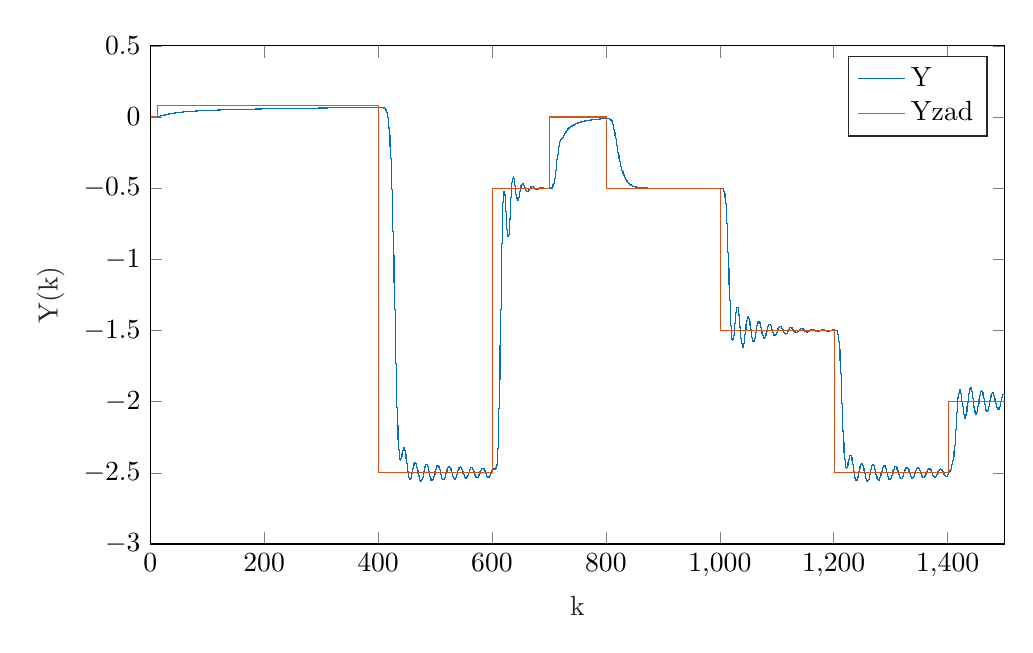
\begin{tikzpicture}

\begin{axis}[%
width=4.272in,
height=2.491in,
at={(0.717in,0.423in)},
scale only axis,
xmin=0,
xmax=1500,
xlabel style={font=\color{white!15!black}},
xlabel={k},
ymin=-3,
ymax=0.5,
ylabel style={font=\color{white!15!black}},
ylabel={Y(k)},
axis background/.style={fill=white},
legend style={legend cell align=left, align=left, draw=white!15!black}
]
\addplot[const plot, color=mycolor1] table[row sep=crcr] {%
1	0\\
2	0\\
3	0\\
4	0\\
5	0\\
6	0\\
7	0\\
8	0\\
9	0\\
10	0\\
11	0\\
12	0\\
13	0\\
14	0\\
15	0\\
16	0\\
17	0.00334251881758044\\
18	0.00765534463299018\\
19	0.00965804373695366\\
20	0.0106757305995262\\
21	0.0114241496148576\\
22	0.012084193643498\\
23	0.0126472821521787\\
24	0.0132737476940759\\
25	0.0140796418301941\\
26	0.0150176572075017\\
27	0.0160122510718432\\
28	0.0170128226148723\\
29	0.0179899431536813\\
30	0.0189231591155231\\
31	0.019803986825167\\
32	0.0206359757368321\\
33	0.021427558537446\\
34	0.0221867679209937\\
35	0.0229195863130518\\
36	0.0236299640753066\\
37	0.0243200550428417\\
38	0.0249907031533228\\
39	0.0256421271255527\\
40	0.0262744536122764\\
41	0.0268879684705007\\
42	0.0274831685519479\\
43	0.0280607229484273\\
44	0.0286213996010176\\
45	0.0291659895647497\\
46	0.0296952523150471\\
47	0.0302098892394284\\
48	0.03071053893\\
49	0.0311977841812393\\
50	0.0316721630099778\\
51	0.0321341791222243\\
52	0.0325843096328277\\
53	0.0330230096627306\\
54	0.0334507145376364\\
55	0.0338678406229964\\
56	0.0342747856386982\\
57	0.0346719289618917\\
58	0.0350596321363446\\
59	0.0354382396118389\\
60	0.0358080796383131\\
61	0.0361694652165408\\
62	0.0365226950277235\\
63	0.0368680542981368\\
64	0.0372058155841027\\
65	0.0375362394810182\\
66	0.0378595752684321\\
67	0.0381760615042456\\
68	0.0384859265785195\\
69	0.0387893892338201\\
70	0.0390866590560833\\
71	0.0393779369381132\\
72	0.0396634155169599\\
73	0.0399432795861964\\
74	0.040217706484212\\
75	0.0404868664598041\\
76	0.0407509230164637\\
77	0.041010033236774\\
78	0.0412643480882897\\
79	0.0415140127121686\\
80	0.0417591666957164\\
81	0.0419999443298997\\
82	0.0422364748527886\\
83	0.0424688826798126\\
84	0.0426972876216451\\
85	0.0429218050904771\\
86	0.0431425462953877\\
87	0.0433596184274724\\
88	0.0435731248353459\\
89	0.0437831651915959\\
90	0.0439898356507248\\
91	0.0441932289990805\\
92	0.0443934347972442\\
93	0.0445905395153132\\
94	0.0447846266614849\\
95	0.0449757769043267\\
96	0.045164068189086\\
97	0.0453495758483776\\
98	0.0455323727075597\\
99	0.0457125291850932\\
100	0.0458901133881596\\
101	0.0460651912037947\\
102	0.0462378263857826\\
103	0.0464080806375346\\
104	0.0465760136911699\\
105	0.0467416833829967\\
106	0.0469051457255838\\
107	0.0470664549766004\\
108	0.0472256637045904\\
109	0.0473828228518401\\
110	0.0475379817944865\\
111	0.0476911884000064\\
112	0.0478424890822187\\
113	0.0479919288539222\\
114	0.048139551377289\\
115	0.0482853990121219\\
116	0.048429512862081\\
117	0.0485719328189788\\
118	0.0487126976052365\\
119	0.0488518448145891\\
120	0.0489894109511249\\
121	0.0491254314667353\\
122	0.049259940797052\\
123	0.0493929723959412\\
124	0.0495245587686222\\
125	0.0496547315034729\\
126	0.049783521302584\\
127	0.0499109580111176\\
128	0.0500370706455242\\
129	0.0501618874206707\\
130	0.0502854357759264\\
131	0.0504077424002544\\
132	0.0505288332563524\\
133	0.0506487336038828\\
134	0.0507674680218347\\
135	0.0508850604300528\\
136	0.0510015341099697\\
137	0.0511169117245774\\
138	0.0512312153376676\\
139	0.0513444664323735\\
140	0.0514566859290426\\
141	0.051567894202467\\
142	0.0516781110984992\\
143	0.0517873559500785\\
144	0.0518956475926913\\
145	0.0520030043792899\\
146	0.0521094441946903\\
147	0.0522149844694711\\
148	0.0523196421933929\\
149	0.0524234339283573\\
150	0.0525263758209241\\
151	0.052628483614404\\
152	0.0527297726605436\\
153	0.0528302579308175\\
154	0.0529299540273445\\
155	0.053028875193441\\
156	0.0531270353238265\\
157	0.053224447974493\\
158	0.0533211263722529\\
159	0.0534170834239763\\
160	0.0535123317255295\\
161	0.0536068835704262\\
162	0.0537007509582016\\
163	0.0537939456025202\\
164	0.0538864789390267\\
165	0.0539783621329492\\
166	0.0540696060864639\\
167	0.0541602214458306\\
168	0.0542502186083054\\
169	0.054339607728841\\
170	0.0544283987265802\\
171	0.0545166012911504\\
172	0.0546042248887671\\
173	0.0546912787681512\\
174	0.0547777719662693\\
175	0.0548637133138998\\
176	0.0549491114410333\\
177	0.0550339747821129\\
178	0.0551183115811177\\
179	0.0552021298964979\\
180	0.0552854376059634\\
181	0.0553682424111338\\
182	0.0554505518420522\\
183	0.0555323732615679\\
184	0.0556137138695935\\
185	0.0556945807072388\\
186	0.055774980660827\\
187	0.0558549204657959\\
188	0.0559344067104885\\
189	0.056013445839837\\
190	0.0560920441589423\\
191	0.0561702078365539\\
192	0.0562479429084515\\
193	0.0563252552807341\\
194	0.0564021507330168\\
195	0.0564786349215396\\
196	0.056554713382191\\
197	0.0566303915334489\\
198	0.0567056746792406\\
199	0.0567805680117259\\
200	0.0568550766140044\\
201	0.0569292054627497\\
202	0.0570029594307729\\
203	0.0570763432895177\\
204	0.0571493617114887\\
205	0.0572220192726147\\
206	0.0572943204545505\\
207	0.0573662696469165\\
208	0.0574378711494808\\
209	0.0575091291742829\\
210	0.0575800478477024\\
211	0.0576506312124743\\
212	0.0577208832296507\\
213	0.0577908077805132\\
214	0.057860408668435\\
215	0.0579296896206954\\
216	0.0579986542902479\\
217	0.0580673062574429\\
218	0.058135649031707\\
219	0.058203686053179\\
220	0.058271420694305\\
221	0.0583388562613932\\
222	0.0584059959961291\\
223	0.0584728430770535\\
224	0.0585394006210026\\
225	0.0586056716845131\\
226	0.0586716592651917\\
227	0.0587373663030509\\
228	0.0588027956818117\\
229	0.0588679502301743\\
230	0.0589328327230574\\
231	0.058997445882807\\
232	0.059061792380376\\
233	0.0591258748364747\\
234	0.0591896958226934\\
235	0.0592532578625977\\
236	0.0593165634327976\\
237	0.05937961496399\\
238	0.0594424148419774\\
239	0.0595049654086604\\
240	0.0595672689630081\\
241	0.0596293277620042\\
242	0.0596911440215708\\
243	0.0597527199174706\\
244	0.059814057586187\\
245	0.0598751591257837\\
246	0.0599360265967445\\
247	0.0599966620227922\\
248	0.060057067391689\\
249	0.060117244656018\\
250	0.0601771957339463\\
251	0.0602369225099701\\
252	0.0602964268356427\\
253	0.0603557105302857\\
254	0.0604147753816828\\
255	0.0604736231467585\\
256	0.0605322555522409\\
257	0.0605906742953085\\
258	0.0606488810442231\\
259	0.0607068774389472\\
260	0.0607646650917481\\
261	0.0608222455877874\\
262	0.0608796204856972\\
263	0.0609367913181437\\
264	0.0609937595923774\\
265	0.0610505267907707\\
266	0.0611070943713436\\
267	0.0611634637682775\\
268	0.0612196363924171\\
269	0.0612756136317611\\
270	0.061331396851942\\
271	0.0613869873966948\\
272	0.0614423865883155\\
273	0.0614975957281088\\
274	0.0615526160968262\\
275	0.0616074489550942\\
276	0.061662095543833\\
277	0.0617165570846657\\
278	0.0617708347803183\\
279	0.061824929815011\\
280	0.061878843354841\\
281	0.0619325765481563\\
282	0.0619861305259217\\
283	0.0620395064020764\\
284	0.0620927052738838\\
285	0.0621457282222734\\
286	0.0621985763121759\\
287	0.06225125059285\\
288	0.0623037520982023\\
289	0.0623560818471007\\
290	0.0624082408436803\\
291	0.0624602300776427\\
292	0.0625120505245493\\
293	0.0625637031461075\\
294	0.062615188890451\\
295	0.0626665086924141\\
296	0.0627176634737996\\
297	0.0627686541436417\\
298	0.0628194815984621\\
299	0.0628701467225214\\
300	0.0629206503880649\\
301	0.0629709934555627\\
302	0.0630211767739452\\
303	0.0630712011808328\\
304	0.0631210675027614\\
305	0.0631707765554025\\
306	0.0632203291437789\\
307	0.0632697260624755\\
308	0.0633189680958459\\
309	0.063368056018214\\
310	0.0634169905940722\\
311	0.0634657725782742\\
312	0.0635144027162248\\
313	0.0635628817440649\\
314	0.063611210388853\\
315	0.0636593893687421\\
316	0.063707419393154\\
317	0.0637553011629489\\
318	0.0638030353705918\\
319	0.0638506227003153\\
320	0.063898063828279\\
321	0.0639453594227253\\
322	0.0639925101441322\\
323	0.064039516645363\\
324	0.0640863795718119\\
325	0.0641330995615479\\
326	0.0641796772454544\\
327	0.0642261132473667\\
328	0.0642724081842064\\
329	0.0643185626661126\\
330	0.0643645772965705\\
331	0.0644104526725379\\
332	0.0644561893845683\\
333	0.0645017880169314\\
334	0.0645472491477318\\
335	0.0645925733490242\\
336	0.0646377611869273\\
337	0.0646828132217344\\
338	0.064727730008022\\
339	0.0647725120947562\\
340	0.0648171600253971\\
341	0.0648616743380003\\
342	0.0649060555653171\\
343	0.0649503042348919\\
344	0.0649944208691582\\
345	0.0650384059855323\\
346	0.0650822600965047\\
347	0.0651259837097304\\
348	0.0651695773281166\\
349	0.0652130414499091\\
350	0.0652563765687764\\
351	0.0652995831738922\\
352	0.065342661750017\\
353	0.0653856127775763\\
354	0.0654284367327392\\
355	0.0654711340874935\\
356	0.0655137053097207\\
357	0.0655561508632688\\
358	0.0655984712080231\\
359	0.0656406667999768\\
360	0.0656827380912993\\
361	0.0657246855304025\\
362	0.0657665095620076\\
363	0.0658082106272084\\
364	0.065849789163535\\
365	0.0658912456050149\\
366	0.0659325803822337\\
367	0.0659737939223942\\
368	0.0660148866493745\\
369	0.0660558589837845\\
370	0.0660967113430215\\
371	0.0661374441413249\\
372	0.0661780577898294\\
373	0.066218552696617\\
374	0.0662589292667687\\
375	0.0662991879024141\\
376	0.0663393290027807\\
377	0.0663793529642421\\
378	0.066419260180365\\
379	0.0664590510419553\\
380	0.0664987259371033\\
381	0.0665382852512283\\
382	0.0665777293671213\\
383	0.0666170586649883\\
384	0.0666562735224915\\
385	0.0666953743147898\\
386	0.0667343614145794\\
387	0.0667732351921324\\
388	0.0668119960153357\\
389	0.0668506442497278\\
390	0.0668891802585362\\
391	0.0669276044027134\\
392	0.0669659170409719\\
393	0.0670041185298192\\
394	0.0670422092235914\\
395	0.0670801894744864\\
396	0.0671180596325969\\
397	0.0671558200459418\\
398	0.0671934710604976\\
399	0.0672310130202291\\
400	0.0672684462671192\\
401	0.0673057711411987\\
402	0.0673429879805745\\
403	0.0673800971214583\\
404	0.0674170988981942\\
405	0.0674539936432856\\
406	0.0672873865704832\\
407	0.0661740399528626\\
408	0.0663210994159769\\
409	0.0652991642119471\\
410	0.0631766312644016\\
411	0.060239001287069\\
412	0.0564930462125625\\
413	0.0515561085784237\\
414	0.044609031712431\\
415	0.0343733236146652\\
416	0.0191413165408592\\
417	-0.00311569161245602\\
418	-0.0345692778530861\\
419	-0.077326895739846\\
420	-0.133249129336811\\
421	-0.203830933563493\\
422	-0.290159957563178\\
423	-0.392940563966156\\
424	-0.512558664257264\\
425	-0.649160591047823\\
426	-0.802724868319318\\
427	-0.973114167842658\\
428	-1.15958265871402\\
429	-1.35545845544792\\
430	-1.5493146725896\\
431	-1.73193057610853\\
432	-1.89785408294498\\
433	-2.04378231358622\\
434	-2.16651109457547\\
435	-2.26386310662547\\
436	-2.33541383076289\\
437	-2.38220569969397\\
438	-2.4064495130758\\
439	-2.41161069779283\\
440	-2.40230364022773\\
441	-2.38383524502363\\
442	-2.361675947578\\
443	-2.34098868522646\\
444	-2.32618181624136\\
445	-2.32052870787358\\
446	-2.32593862162308\\
447	-2.34289451998286\\
448	-2.36885932319486\\
449	-2.39979181308193\\
450	-2.43238860708304\\
451	-2.46440522834943\\
452	-2.49345894166747\\
453	-2.51721647034676\\
454	-2.53403042337497\\
455	-2.54305350304249\\
456	-2.54408374243988\\
457	-2.53759755601181\\
458	-2.52479926062325\\
459	-2.50749203695571\\
460	-2.48785023182906\\
461	-2.46819731270607\\
462	-2.45078143861437\\
463	-2.43754383539099\\
464	-2.42992341668752\\
465	-2.42873136360109\\
466	-2.43409740718401\\
467	-2.44548187979225\\
468	-2.46174979572417\\
469	-2.48129778034601\\
470	-2.50221837418266\\
471	-2.5224858377125\\
472	-2.54014916901591\\
473	-2.55351790662473\\
474	-2.56132557453657\\
475	-2.56285592281662\\
476	-2.55801849950281\\
477	-2.54736287102866\\
478	-2.53202595937415\\
479	-2.51361472681722\\
480	-2.49403560820712\\
481	-2.47529050660601\\
482	-2.45926456138443\\
483	-2.44753173421377\\
484	-2.44120042613269\\
485	-2.44081419691293\\
486	-2.44631430629542\\
487	-2.45706312180037\\
488	-2.47192154887579\\
489	-2.4893698221107\\
490	-2.50765895722261\\
491	-2.52497933131184\\
492	-2.53963264761846\\
493	-2.55019355284251\\
494	-2.55564733509401\\
495	-2.55549073335769\\
496	-2.54978452233206\\
497	-2.53914985177375\\
498	-2.52470567653545\\
499	-2.50795170750157\\
500	-2.49060899903477\\
501	-2.47443680213074\\
502	-2.46104790962617\\
503	-2.45174443212379\\
504	-2.44739200365848\\
505	-2.44834408572438\\
506	-2.45442098385099\\
507	-2.46494182777497\\
508	-2.47880289812622\\
509	-2.49459248913884\\
510	-2.51073072535619\\
511	-2.52562195502489\\
512	-2.53780709543432\\
513	-2.54610335301234\\
514	-2.54971910137989\\
515	-2.54833267165928\\
516	-2.54212586677371\\
517	-2.53176658884647\\
518	-2.51834016479369\\
519	-2.50323528443066\\
520	-2.48799681683088\\
521	-2.47416268742924\\
522	-2.4631042170571\\
523	-2.45588830723283\\
524	-2.4531760042643\\
525	-2.45516639977299\\
526	-2.46158885120944\\
527	-2.47174120180332\\
528	-2.4845676271319\\
529	-2.49876704410904\\
530	-2.51292147798361\\
531	-2.52563305400073\\
532	-2.53565805901246\\
533	-2.54202665863302\\
534	-2.54413743031141\\
535	-2.54181715412775\\
536	-2.53533864918181\\
537	-2.52539310039982\\
538	-2.51301819753699\\
539	-2.49948892896359\\
540	-2.48618302275376\\
541	-2.47443664156978\\
542	-2.46540713310466\\
543	-2.45995817087429\\
544	-2.45857896451719\\
545	-2.46134433078819\\
546	-2.46791734495514\\
547	-2.47759184753735\\
548	-2.48936868695437\\
549	-2.50205729950092\\
550	-2.51439289548552\\
551	-2.52515888151897\\
552	-2.53330399717051\\
553	-2.53804390889407\\
554	-2.53893778352432\\
555	-2.53593188638439\\
556	-2.52936476041486\\
557	-2.51993213737694\\
558	-2.50861419174129\\
559	-2.49657247078201\\
560	-2.48502793348625\\
561	-2.47513410107893\\
562	-2.46785977228555\\
563	-2.46389403660434\\
564	-2.46358291720214\\
565	-2.46690270097061\\
566	-2.47347069663454\\
567	-2.48259041923363\\
568	-2.49332534161925\\
569	-2.50459341945761\\
570	-2.51527345460172\\
571	-2.52431383011797\\
572	-2.53083409534573\\
573	-2.53421027993659\\
574	-2.53413577414148\\
575	-2.53065130498955\\
576	-2.52414010900295\\
577	-2.51528783043531\\
578	-2.50501066488878\\
579	-2.49435923884493\\
580	-2.48440891661922\\
581	-2.47614897357951\\
582	-2.47038299478194\\
583	-2.46765102233612\\
584	-2.46818085232625\\
585	-2.47187215056008\\
586	-2.47831337258197\\
587	-2.48682830901156\\
588	-2.49654666281862\\
589	-2.50649142502933\\
590	-2.51567485179824\\
591	-2.52319443188587\\
592	-2.52832028917607\\
593	-2.530565997909\\
594	-2.52973589062697\\
595	-2.52594373251701\\
596	-2.5196001805512\\
597	-2.51136963716639\\
598	-2.50210061447286\\
599	-2.49273700968408\\
600	-2.48422014021375\\
601	-2.47739249535708\\
602	-2.47291371538298\\
603	-2.47119745004011\\
604	-2.47237490980456\\
605	-2.47628766781592\\
606	-2.46714111782085\\
607	-2.46009012212696\\
608	-2.44474797128605\\
609	-2.40406287763767\\
610	-2.32729096755526\\
611	-2.20882898578684\\
612	-2.04734766022963\\
613	-1.8452306575032\\
614	-1.60834298021668\\
615	-1.35392414578779\\
616	-1.10645091632958\\
617	-0.889084440393151\\
618	-0.717845851136\\
619	-0.600520927496247\\
620	-0.53742241485493\\
621	-0.523095740091871\\
622	-0.548063624889165\\
623	-0.600409451812301\\
624	-0.667129078176472\\
625	-0.735301224168847\\
626	-0.793140475194513\\
627	-0.831002956300024\\
628	-0.842387876897563\\
629	-0.824871307159524\\
630	-0.78070093586581\\
631	-0.716588564841342\\
632	-0.642361594700348\\
633	-0.568722531471029\\
634	-0.504975558548587\\
635	-0.457557656907005\\
636	-0.429596728460974\\
637	-0.421183897530055\\
638	-0.429973380754134\\
639	-0.451895927294034\\
640	-0.481893989220814\\
641	-0.51462037179827\\
642	-0.545062204762461\\
643	-0.569072959822202\\
644	-0.583793540028699\\
645	-0.587923404639346\\
646	-0.581790374354859\\
647	-0.567182064340102\\
648	-0.54694742965072\\
649	-0.524441503731638\\
650	-0.502937507778997\\
651	-0.485134406652173\\
652	-0.472842252221098\\
653	-0.466863956048907\\
654	-0.467044743693581\\
655	-0.472440753429756\\
656	-0.481557774333273\\
657	-0.492618396446553\\
658	-0.503824330217936\\
659	-0.513587926959672\\
660	-0.520712520063574\\
661	-0.52450606717785\\
662	-0.524818578265492\\
663	-0.522002398342764\\
664	-0.516805299441158\\
665	-0.510217202078006\\
666	-0.503298725739765\\
667	-0.497020899200945\\
668	-0.492139885565005\\
669	-0.489120757347824\\
670	-0.488113653561422\\
671	-0.488976882022885\\
672	-0.491335942337998\\
673	-0.494664923276486\\
674	-0.498376514334669\\
675	-0.501908161189655\\
676	-0.504794115537469\\
677	-0.506715967267743\\
678	-0.507527534429299\\
679	-0.507253543794598\\
680	-0.506065044185178\\
681	-0.504237486047896\\
682	-0.502099366079847\\
683	-0.499979917321947\\
684	-0.498163472979447\\
685	-0.496856137069384\\
686	-0.496167779774327\\
687	-0.49610971065049\\
688	-0.496606124209978\\
689	-0.497515822614893\\
690	-0.498659877318563\\
691	-0.499850744607777\\
692	-0.500918780589521\\
693	-0.501732965019168\\
694	-0.50221378902101\\
695	-0.502337533693015\\
696	-0.502132406055676\\
697	-0.50166805227933\\
698	-0.50104070623567\\
699	-0.500356572749267\\
700	-0.499715974213724\\
701	-0.499200360643625\\
702	-0.498863605793054\\
703	-0.498728222315456\\
704	-0.49878636110492\\
705	-0.499004821600688\\
706	-0.485269227241348\\
707	-0.474731151311315\\
708	-0.466390885464399\\
709	-0.453501669631161\\
710	-0.432750069743442\\
711	-0.406250017650789\\
712	-0.374724829443278\\
713	-0.33900057490768\\
714	-0.301720051949728\\
715	-0.266198454046441\\
716	-0.234768019537164\\
717	-0.208723317767813\\
718	-0.188555279647637\\
719	-0.173925605232924\\
720	-0.16377761763219\\
721	-0.156705542775103\\
722	-0.151308392075714\\
723	-0.146405806081039\\
724	-0.141169312316397\\
725	-0.135185388560321\\
726	-0.128424582661861\\
727	-0.121132712767768\\
728	-0.113694100229032\\
729	-0.106506118477956\\
730	-0.0998859799711665\\
731	-0.0940203985898193\\
732	-0.0889581313933497\\
733	-0.0846346347016253\\
734	-0.0809134561423288\\
735	-0.0776305355601038\\
736	-0.0746314727344393\\
737	-0.0717960725915862\\
738	-0.0690486960137356\\
739	-0.0663564470296406\\
740	-0.063719281055915\\
741	-0.0611566246281768\\
742	-0.0586944435226508\\
743	-0.0563553797393714\\
744	-0.0541530747853634\\
745	-0.0520905106397584\\
746	-0.0501613701616983\\
747	-0.0483530888552215\\
748	-0.0466503452730404\\
749	-0.0450380647157064\\
750	-0.0435034336654653\\
751	-0.0420368141694047\\
752	-0.0406317303521107\\
753	-0.0392842465447203\\
754	-0.037992081317498\\
755	-0.0367537404687244\\
756	-0.0355678483867183\\
757	-0.0344327495516907\\
758	-0.0333463662579747\\
759	-0.032306246681058\\
760	-0.0313097189979548\\
761	-0.0303540745524591\\
762	-0.0294367251011349\\
763	-0.0285553055920365\\
764	-0.0277077170862898\\
765	-0.0268921202333123\\
766	-0.0261068972501258\\
767	-0.0253506009671279\\
768	-0.0246219056259316\\
769	-0.0239195683197636\\
770	-0.0232424043083756\\
771	-0.0225892751705473\\
772	-0.0219590863374877\\
773	-0.0213507898368808\\
774	-0.0207633885854113\\
775	-0.0201959397136573\\
776	-0.0196475556823029\\
777	-0.0191174030088573\\
778	-0.0186046991077538\\
779	-0.018108708042092\\
780	-0.0176287359754935\\
781	-0.0171641269194351\\
782	-0.016714259112059\\
783	-0.0162785421255524\\
784	-0.0158564146286529\\
785	-0.0154473426417467\\
786	-0.0150508181032255\\
787	-0.0146663575940551\\
788	-0.0142935011178006\\
789	-0.0139318108853661\\
790	-0.0135808700947956\\
791	-0.0132402817215793\\
792	-0.0129096673447217\\
793	-0.0125886660323344\\
794	-0.0122769333027496\\
795	-0.0119741401675743\\
796	-0.0116799722548034\\
797	-0.0113941290046078\\
798	-0.011116322927951\\
799	-0.010846278918189\\
800	-0.0105837336073388\\
801	-0.0103284347608395\\
802	-0.0100801407066871\\
803	-0.00983861979640084\\
804	-0.00960364989624252\\
805	-0.00937501790754354\\
806	-0.0136564313890633\\
807	-0.0171789829648189\\
808	-0.0184595595847671\\
809	-0.021551605590909\\
810	-0.0280122848680496\\
811	-0.0378143665584065\\
812	-0.0507558086058294\\
813	-0.0669393494812172\\
814	-0.0860499037218895\\
815	-0.107408541450966\\
816	-0.130342434329158\\
817	-0.154270132559772\\
818	-0.178627300526582\\
819	-0.202882864634861\\
820	-0.226602843679299\\
821	-0.249458799281784\\
822	-0.27120653214029\\
823	-0.291678557690517\\
824	-0.310782258807891\\
825	-0.328487604636425\\
826	-0.344810408459733\\
827	-0.359799355982691\\
828	-0.373525493193285\\
829	-0.386071856252021\\
830	-0.397524683760667\\
831	-0.40796760004832\\
832	-0.417478232958771\\
833	-0.426126520051608\\
834	-0.433974542445737\\
835	-0.441077624913433\\
836	-0.447486110559279\\
837	-0.45324727173134\\
838	-0.458407027291708\\
839	-0.463011229756976\\
840	-0.467106351411621\\
841	-0.470739525769491\\
842	-0.473958027061812\\
843	-0.476808342052705\\
844	-0.479335022145767\\
845	-0.481579515965709\\
846	-0.483579166333993\\
847	-0.485366510704005\\
848	-0.486968964696384\\
849	-0.488408907103609\\
850	-0.489704128532154\\
851	-0.490868560788594\\
852	-0.491913175755686\\
853	-0.492846932982344\\
854	-0.493677663066377\\
855	-0.494412795743024\\
856	-0.495059872885571\\
857	-0.495626822048383\\
858	-0.496122000384026\\
859	-0.496554047272266\\
860	-0.496931603715572\\
861	-0.497262965940083\\
862	-0.49755573972372\\
863	-0.497816552196748\\
864	-0.498050861701985\\
865	-0.498262886788116\\
866	-0.498455655629728\\
867	-0.49863115984883\\
868	-0.498790583891942\\
869	-0.498934573951963\\
870	-0.499063509151451\\
871	-0.499177741729137\\
872	-0.499277781057677\\
873	-0.499364406838829\\
874	-0.499438708022937\\
875	-0.499502054264947\\
876	-0.499556014776576\\
877	-0.4996022444475\\
878	-0.499642358790305\\
879	-0.499677817810653\\
880	-0.49970983491536\\
881	-0.499739321316325\\
882	-0.499766870052774\\
883	-0.499792777689455\\
884	-0.499817096745619\\
885	-0.499839708512991\\
886	-0.49986040438526\\
887	-0.499878964114704\\
888	-0.499895221256418\\
889	-0.499909109004317\\
890	-0.499920683121515\\
891	-0.499930122171193\\
892	-0.499937708283286\\
893	-0.499943793894137\\
894	-0.499948761076276\\
895	-0.499952980203709\\
896	-0.499956773892102\\
897	-0.49996039064329\\
898	-0.499963990706198\\
899	-0.499967644655617\\
900	-0.499971343372712\\
901	-0.4999750167096\\
902	-0.499978557272292\\
903	-0.499981845505904\\
904	-0.499984772570213\\
905	-0.499987258239128\\
906	-0.499989262085694\\
907	-0.499990787347946\\
908	-0.499991877941781\\
909	-0.499992609956859\\
910	-0.499993079547479\\
911	-0.499993389371516\\
912	-0.499993635647156\\
913	-0.499993897542338\\
914	-0.499994230069081\\
915	-0.499994661022394\\
916	-0.499995191879206\\
917	-0.499995802040864\\
918	-0.499996455423822\\
919	-0.499997108209247\\
920	-0.499997716555915\\
921	-0.499998243238655\\
922	-0.499998662453929\\
923	-0.499998962381138\\
924	-0.49999914544676\\
925	-0.499999226558058\\
926	-0.499999229815158\\
927	-0.499999184351762\\
928	-0.499999119989316\\
929	-0.499999063326037\\
930	-0.499999034742272\\
931	-0.499999046616035\\
932	-0.499999102839093\\
933	-0.499999199534426\\
934	-0.499999326724388\\
935	-0.499999470601166\\
936	-0.499999616013625\\
937	-0.499999748804656\\
938	-0.499999857700563\\
939	-0.499999935553536\\
940	-0.499999979852093\\
941	-0.499999992525158\\
942	-0.499999979158498\\
943	-0.499999947807021\\
944	-0.499999907617893\\
945	-0.499999867477449\\
946	-0.499999834864088\\
947	-0.499999815037667\\
948	-0.499999810633082\\
949	-0.499999821661756\\
950	-0.499999845868554\\
951	-0.499999879349844\\
952	-0.499999917314891\\
953	-0.499999954868384\\
954	-0.499999987704724\\
955	-0.500000012630858\\
956	-0.500000027868527\\
957	-0.500000033123281\\
958	-0.500000029441015\\
959	-0.500000018899152\\
960	-0.500000004196045\\
961	-0.499999988207878\\
962	-0.499999973577823\\
963	-0.499999962389464\\
964	-0.499999955958257\\
965	-0.499999954754332\\
966	-0.499999958450291\\
967	-0.499999966071389\\
968	-0.499999976214429\\
969	-0.499999987296661\\
970	-0.499999997796861\\
971	-0.50000000645671\\
972	-0.500000012420122\\
973	-0.500000015299524\\
974	-0.500000015169483\\
975	-0.50000001249792\\
976	-0.500000008032396\\
977	-0.500000002662763\\
978	-0.499999997282034\\
979	-0.499999992664669\\
980	-0.499999989376689\\
981	-0.499999987725764\\
982	-0.499999987752966\\
983	-0.499999989261932\\
984	-0.499999991876635\\
985	-0.499999995116197\\
986	-0.499999998474338\\
987	-0.500000001492008\\
988	-0.500000003814185\\
989	-0.500000005225113\\
990	-0.500000005659964\\
991	-0.500000005194374\\
992	-0.50000000401613\\
993	-0.500000002385182\\
994	-0.500000000588952\\
995	-0.499999998899637\\
996	-0.499999997539095\\
997	-0.499999996655118\\
998	-0.499999996310871\\
999	-0.499999996487237\\
1000	-0.499999997096094\\
1001	-0.499999998001287\\
1002	-0.499999999043452\\
1003	-0.500000000064803\\
1004	-0.500000000930501\\
1005	-0.500000001544131\\
1006	-0.5124154420226\\
1007	-0.522500173215759\\
1008	-0.535957142532218\\
1009	-0.562716918369215\\
1010	-0.607455139344931\\
1011	-0.669758548881221\\
1012	-0.749112707078841\\
1013	-0.844164347638534\\
1014	-0.951146162033024\\
1015	-1.06458678965584\\
1016	-1.17854604668329\\
1017	-1.28700166064505\\
1018	-1.38401308746655\\
1019	-1.46427381053525\\
1020	-1.52374596130775\\
1021	-1.56008148586118\\
1022	-1.57290133409814\\
1023	-1.56397967914012\\
1024	-1.53718743291079\\
1025	-1.49808744056597\\
1026	-1.45323559286689\\
1027	-1.40932957023821\\
1028	-1.37236943494172\\
1029	-1.3469878540253\\
1030	-1.3360480240498\\
1031	-1.34051773754045\\
1032	-1.35956861354681\\
1033	-1.3908359197157\\
1034	-1.43078244292043\\
1035	-1.47512105088246\\
1036	-1.51926154499796\\
1037	-1.55875671439097\\
1038	-1.58972676657886\\
1039	-1.60923919489519\\
1040	-1.61561446662667\\
1041	-1.60862029802324\\
1042	-1.58951433218696\\
1043	-1.56090440438521\\
1044	-1.52642290077704\\
1045	-1.49025333859617\\
1046	-1.45658724065026\\
1047	-1.42910746169111\\
1048	-1.41058097672631\\
1049	-1.40260860235878\\
1050	-1.40554013518476\\
1051	-1.41853557436526\\
1052	-1.43974004557647\\
1053	-1.46653782594462\\
1054	-1.49585408623825\\
1055	-1.52447765169409\\
1056	-1.54938182237482\\
1057	-1.56802187430615\\
1058	-1.57858725399096\\
1059	-1.58018490325952\\
1060	-1.57293002087115\\
1061	-1.55792504341184\\
1062	-1.53711932970431\\
1063	-1.51306087867231\\
1064	-1.4885729493379\\
1065	-1.46640486561174\\
1066	-1.44891060435603\\
1067	-1.43779941514147\\
1068	-1.43398444216433\\
1069	-1.43753564710082\\
1070	-1.44772804231447\\
1071	-1.46316731746094\\
1072	-1.48197142752187\\
1073	-1.50198655058579\\
1074	-1.52101709671281\\
1075	-1.53705083597881\\
1076	-1.54846112069228\\
1077	-1.55416875977575\\
1078	-1.5537472022041\\
1079	-1.54745758760479\\
1080	-1.53620614959558\\
1081	-1.5214257912036\\
1082	-1.5048951854242\\
1083	-1.4885196183568\\
1084	-1.47410449719321\\
1085	-1.46315265469476\\
1086	-1.45671042192028\\
1087	-1.45527733615872\\
1088	-1.458783571947\\
1089	-1.46663026744829\\
1090	-1.47778194972683\\
1091	-1.49089708488929\\
1092	-1.50448161608403\\
1093	-1.51705034771369\\
1094	-1.52728156741546\\
1095	-1.53415112020582\\
1096	-1.5370334013021\\
1097	-1.53575884892218\\
1098	-1.53062100835155\\
1099	-1.52233137311549\\
1100	-1.51192667746205\\
1101	-1.50064006632483\\
1102	-1.48975302964679\\
1103	-1.48044765514645\\
1104	-1.47367788633891\\
1105	-1.47007443990609\\
1106	-1.46989209890315\\
1107	-1.47300179481753\\
1108	-1.47892443925606\\
1109	-1.48689947474854\\
1110	-1.49597863958018\\
1111	-1.50513421594487\\
1112	-1.51337070367081\\
1113	-1.5198291689302\\
1114	-1.52387436063806\\
1115	-1.52515613324566\\
1116	-1.52363891895074\\
1117	-1.51959606490033\\
1118	-1.51356969942154\\
1119	-1.50630101109567\\
1120	-1.49863971546004\\
1121	-1.4914442327288\\
1122	-1.48548507067318\\
1123	-1.48136289891444\\
1124	-1.47945012523217\\
1125	-1.47986112077882\\
1126	-1.48245236784179\\
1127	-1.48685035102089\\
1128	-1.49250233951711\\
1129	-1.49874341477091\\
1130	-1.50487211668712\\
1131	-1.51022678594593\\
1132	-1.51425496360007\\
1133	-1.51656902551601\\
1134	-1.51698258231372\\
1135	-1.51552407345218\\
1136	-1.51242637098843\\
1137	-1.50809390281735\\
1138	-1.50305148024038\\
1139	-1.49788124632488\\
1140	-1.49315553912434\\
1141	-1.48937372355251\\
1142	-1.48691016281009\\
1143	-1.48597869454091\\
1144	-1.48661663075244\\
1145	-1.48868883432377\\
1146	-1.49191018770912\\
1147	-1.4958829828526\\
1148	-1.50014452024581\\
1149	-1.50421951480387\\
1150	-1.50767172960687\\
1151	-1.51014955232988\\
1152	-1.51142095959626\\
1153	-1.5113944501346\\
1154	-1.5101240157106\\
1155	-1.50779795679349\\
1156	-1.50471316837755\\
1157	-1.50123819249982\\
1158	-1.49776961088149\\
1159	-1.49468702830066\\
1160	-1.49231186947913\\
1161	-1.49087450580068\\
1162	-1.49049299131899\\
1163	-1.49116514482638\\
1164	-1.49277410672654\\
1165	-1.4951060310819\\
1166	-1.49787738635325\\
1167	-1.50076850937347\\
1168	-1.50345961137431\\
1169	-1.50566536663426\\
1170	-1.50716450207723\\
1171	-1.50782141877606\\
1172	-1.50759776918116\\
1173	-1.50655301933145\\
1174	-1.50483424408695\\
1175	-1.50265660475788\\
1176	-1.50027699338081\\
1177	-1.49796405500388\\
1178	-1.49596811638028\\
1179	-1.4944944184627\\
1180	-1.4936825067982\\
1181	-1.49359377755799\\
1182	-1.49420814471631\\
1183	-1.4954297303171\\
1184	-1.49710051085438\\
1185	-1.49902007140511\\
1186	-1.50096908197487\\
1187	-1.50273384305613\\
1188	-1.50412925185631\\
1189	-1.50501780225082\\
1190	-1.50532272104909\\
1191	-1.50503401599506\\
1192	-1.50420700475258\\
1193	-1.50295372885854\\
1194	-1.50142843939877\\
1195	-1.49980897755118\\
1196	-1.49827628283928\\
1197	-1.49699439452919\\
1198	-1.49609315721157\\
1199	-1.49565543261594\\
1200	-1.4957100229293\\
1201	-1.49623081307439\\
1202	-1.4971419307895\\
1203	-1.4983280839435\\
1204	-1.49964872567859\\
1205	-1.50095435960312\\
1206	-1.51584270427097\\
1207	-1.52926201441036\\
1208	-1.54692346365433\\
1209	-1.57966976380951\\
1210	-1.63324642799334\\
1211	-1.70770222472494\\
1212	-1.80141562615716\\
1213	-1.90567081956291\\
1214	-2.0114817868752\\
1215	-2.11289505816612\\
1216	-2.20624409404863\\
1217	-2.2881387015487\\
1218	-2.3556569648202\\
1219	-2.40719014694759\\
1220	-2.44238751912099\\
1221	-2.46184466166867\\
1222	-2.46713218501958\\
1223	-2.46083147016039\\
1224	-2.44628662304078\\
1225	-2.4272354420858\\
1226	-2.40746899132715\\
1227	-2.39049615330888\\
1228	-2.37921327711775\\
1229	-2.37564993861434\\
1230	-2.38083211375813\\
1231	-2.39475338902545\\
1232	-2.41597540278687\\
1233	-2.44139662550514\\
1234	-2.46826185187298\\
1235	-2.49451216292616\\
1236	-2.51801214365053\\
1237	-2.53667669536972\\
1238	-2.54900509190617\\
1239	-2.55422402583435\\
1240	-2.55219300182374\\
1241	-2.54342064347141\\
1242	-2.52908795976861\\
1243	-2.5109261366109\\
1244	-2.49100368078684\\
1245	-2.4715094703123\\
1246	-2.45453602113293\\
1247	-2.44186371594537\\
1248	-2.43478160617972\\
1249	-2.43397373160118\\
1250	-2.43947405133674\\
1251	-2.45068462157702\\
1252	-2.46645211387104\\
1253	-2.48519334920507\\
1254	-2.50505535442418\\
1255	-2.52409476886555\\
1256	-2.54046256326175\\
1257	-2.55257999246479\\
1258	-2.55929121346424\\
1259	-2.55997840777378\\
1260	-2.55462681778206\\
1261	-2.54383017721807\\
1262	-2.52873231254815\\
1263	-2.51090825807626\\
1264	-2.4921968371809\\
1265	-2.47450426929444\\
1266	-2.45960291962609\\
1267	-2.44894955768854\\
1268	-2.44354350483947\\
1269	-2.4438381775495\\
1270	-2.44971170114967\\
1271	-2.46049515812798\\
1272	-2.47505160729875\\
1273	-2.49189548961372\\
1274	-2.50934013618202\\
1275	-2.52566029129017\\
1276	-2.53925633828546\\
1277	-2.54880693708745\\
1278	-2.55339702214381\\
1279	-2.55260887620816\\
1280	-2.54656583824362\\
1281	-2.53592168548184\\
1282	-2.52179409009257\\
1283	-2.50564738690555\\
1284	-2.48913704198981\\
1285	-2.47393403064128\\
1286	-2.46155027917586\\
1287	-2.45318563588053\\
1288	-2.44961284845737\\
1289	-2.45111095930405\\
1290	-2.45745091348323\\
1291	-2.46793126780034\\
1292	-2.48145738940538\\
1293	-2.4966545764795\\
1294	-2.5120038792861\\
1295	-2.52598864275043\\
1296	-2.53723955686492\\
1297	-2.5446660857631\\
1298	-2.5475625991947\\
1299	-2.54567864711866\\
1300	-2.53924503111802\\
1301	-2.528950988719\\
1302	-2.51587292614467\\
1303	-2.50136116867074\\
1304	-2.48689705535799\\
1305	-2.47393704311559\\
1306	-2.46376220835878\\
1307	-2.45735025087233\\
1308	-2.45528326936272\\
1309	-2.4576992529623\\
1310	-2.46428962774897\\
1311	-2.47434026459127\\
1312	-2.48680959888133\\
1313	-2.50043501513683\\
1314	-2.51385721180314\\
1315	-2.52575157858357\\
1316	-2.53495542901212\\
1317	-2.54058012525975\\
1318	-2.54209780045215\\
1319	-2.53939378617979\\
1320	-2.53277830271207\\
1321	-2.52295464543081\\
1322	-2.51094584742607\\
1323	-2.49798701241664\\
1324	-2.48539521959676\\
1325	-2.47443204335389\\
1326	-2.46617455541691\\
1327	-2.46140904068841\\
1328	-2.46055805832076\\
1329	-2.46364682085641\\
1330	-2.47031010327507\\
1331	-2.47983675291072\\
1332	-2.49124571827299\\
1333	-2.50338539665051\\
1334	-2.51504685999392\\
1335	-2.52508093168923\\
1336	-2.53250897952565\\
1337	-2.53661761683268\\
1338	-2.53702836957094\\
1339	-2.53373498282544\\
1340	-2.52710360906209\\
1341	-2.51783468352632\\
1342	-2.50688958843684\\
1343	-2.49538963121028\\
1344	-2.48449857493049\\
1345	-2.47530214960569\\
1346	-2.46869815049363\\
1347	-2.4653089101656\\
1348	-2.46542460734201\\
1349	-2.46898180812708\\
1350	-2.47557758032261\\
1351	-2.48451602937261\\
1352	-2.49488144573687\\
1353	-2.50563045552788\\
1354	-2.51569450911308\\
1355	-2.5240835666424\\
1356	-2.52998183609357\\
1357	-2.53282688309627\\
1358	-2.53236446425981\\
1359	-2.52867319280325\\
1360	-2.52215573472563\\
1361	-2.51349659380942\\
1362	-2.5035903551295\\
1363	-2.49344794702225\\
1364	-2.4840913525219\\
1365	-2.47644864769385\\
1366	-2.47126096804363\\
1367	-2.46901111750945\\
1368	-2.46988050083395\\
1369	-2.47373751277624\\
1370	-2.48015705491385\\
1371	-2.48846789442361\\
1372	-2.49782233069443\\
1373	-2.50728111264685\\
1374	-2.51590566434324\\
1375	-2.52284932002118\\
1376	-2.52743937923056\\
1377	-2.52924238500853\\
1378	-2.52810618943564\\
1379	-2.52417420293164\\
1380	-2.51786975534802\\
1381	-2.50985159541221\\
1382	-2.50094487794069\\
1383	-2.49205501811706\\
1384	-2.48407396278833\\
1385	-2.47778930205928\\
1386	-2.47380606003391\\
1387	-2.47248912770959\\
1388	-2.47393155460641\\
1389	-2.47795082338961\\
1390	-2.48411226779726\\
1391	-2.49177628406066\\
1392	-2.5001640822472\\
1393	-2.50843544060443\\
1394	-2.51577120196909\\
1395	-2.52145301600245\\
1396	-2.52493305258538\\
1397	-2.52588711549846\\
1398	-2.52424583603878\\
1399	-2.52020047516681\\
1400	-2.51418227799392\\
1401	-2.50681712837287\\
1402	-2.49886010364187\\
1403	-2.49111697821384\\
1404	-2.48436132149377\\
1405	-2.47925627435463\\
1406	-2.4606036681944\\
1407	-2.44445503543603\\
1408	-2.43063519832016\\
1409	-2.41237252665862\\
1410	-2.38521299480255\\
1411	-2.35005795449557\\
1412	-2.30672083228208\\
1413	-2.25488909251344\\
1414	-2.19644560481399\\
1415	-2.13516707841645\\
1416	-2.07507792135261\\
1417	-2.02011442408419\\
1418	-1.97406275191228\\
1419	-1.94000641915696\\
1420	-1.9197852396966\\
1421	-1.91388287392732\\
1422	-1.92151205712561\\
1423	-1.94072444350619\\
1424	-1.96860405681834\\
1425	-2.00157439606968\\
1426	-2.03575063236124\\
1427	-2.0672872807069\\
1428	-2.09271745563193\\
1429	-2.10927334717669\\
1430	-2.1151558857299\\
1431	-2.10972084246243\\
1432	-2.09355564687335\\
1433	-2.06842492084259\\
1434	-2.03707401035671\\
1435	-2.00290487484931\\
1436	-1.96956745273027\\
1437	-1.94052867813443\\
1438	-1.9186839603717\\
1439	-1.90606250089906\\
1440	-1.90365459638846\\
1441	-1.91136536337259\\
1442	-1.92808204760351\\
1443	-1.95183294672321\\
1444	-1.98001311006632\\
1445	-2.00965271826473\\
1446	-2.03770614399812\\
1447	-2.0613414699865\\
1448	-2.0782106911523\\
1449	-2.08667988407808\\
1450	-2.08599727570103\\
1451	-2.07637733992892\\
1452	-2.058983269898\\
1453	-2.03580035838208\\
1454	-2.00940882595836\\
1455	-1.98268308361088\\
1456	-1.95845932882509\\
1457	-1.9392190636284\\
1458	-1.92683058074753\\
1459	-1.92237651316184\\
1460	-1.92607878782304\\
1461	-1.9373178149812\\
1462	-1.95473296515234\\
1463	-1.97638635789491\\
1464	-1.9999704217781\\
1465	-2.0230399999922\\
1466	-2.04325062489801\\
1467	-2.05858510508572\\
1468	-2.06755053174102\\
1469	-2.06932770072834\\
1470	-2.06385589676733\\
1471	-2.05183947372911\\
1472	-2.03466987082833\\
1473	-2.01426763226239\\
1474	-1.99286180480992\\
1475	-1.9727353015428\\
1476	-1.95597074677776\\
1477	-1.94422997029657\\
1478	-1.93859249762438\\
1479	-1.93946707938582\\
1480	-1.94657897122952\\
1481	-1.95902670534377\\
1482	-1.97539631368482\\
1483	-1.99391801831268\\
1484	-2.01264939799559\\
1485	-2.02966902535958\\
1486	-2.04326484209416\\
1487	-2.05210180575777\\
1488	-2.05535378523317\\
1489	-2.05278592718235\\
1490	-2.04477662604705\\
1491	-2.03227351569118\\
1492	-2.01668560324083\\
1493	-1.99972275137652\\
1494	-1.98320212605177\\
1495	-1.96884657958131\\
1496	-1.95810061336447\\
1497	-1.95198550549405\\
1498	-1.95100787126483\\
1499	-1.95512753691817\\
1500	-1.96378305919461\\
};
\addlegendentry{Y}

\addplot[const plot, color=mycolor2] table[row sep=crcr] {%
1	0\\
2	0\\
3	0\\
4	0\\
5	0\\
6	0\\
7	0\\
8	0\\
9	0\\
10	0\\
11	0\\
12	0.08\\
13	0.08\\
14	0.08\\
15	0.08\\
16	0.08\\
17	0.08\\
18	0.08\\
19	0.08\\
20	0.08\\
21	0.08\\
22	0.08\\
23	0.08\\
24	0.08\\
25	0.08\\
26	0.08\\
27	0.08\\
28	0.08\\
29	0.08\\
30	0.08\\
31	0.08\\
32	0.08\\
33	0.08\\
34	0.08\\
35	0.08\\
36	0.08\\
37	0.08\\
38	0.08\\
39	0.08\\
40	0.08\\
41	0.08\\
42	0.08\\
43	0.08\\
44	0.08\\
45	0.08\\
46	0.08\\
47	0.08\\
48	0.08\\
49	0.08\\
50	0.08\\
51	0.08\\
52	0.08\\
53	0.08\\
54	0.08\\
55	0.08\\
56	0.08\\
57	0.08\\
58	0.08\\
59	0.08\\
60	0.08\\
61	0.08\\
62	0.08\\
63	0.08\\
64	0.08\\
65	0.08\\
66	0.08\\
67	0.08\\
68	0.08\\
69	0.08\\
70	0.08\\
71	0.08\\
72	0.08\\
73	0.08\\
74	0.08\\
75	0.08\\
76	0.08\\
77	0.08\\
78	0.08\\
79	0.08\\
80	0.08\\
81	0.08\\
82	0.08\\
83	0.08\\
84	0.08\\
85	0.08\\
86	0.08\\
87	0.08\\
88	0.08\\
89	0.08\\
90	0.08\\
91	0.08\\
92	0.08\\
93	0.08\\
94	0.08\\
95	0.08\\
96	0.08\\
97	0.08\\
98	0.08\\
99	0.08\\
100	0.08\\
101	0.08\\
102	0.08\\
103	0.08\\
104	0.08\\
105	0.08\\
106	0.08\\
107	0.08\\
108	0.08\\
109	0.08\\
110	0.08\\
111	0.08\\
112	0.08\\
113	0.08\\
114	0.08\\
115	0.08\\
116	0.08\\
117	0.08\\
118	0.08\\
119	0.08\\
120	0.08\\
121	0.08\\
122	0.08\\
123	0.08\\
124	0.08\\
125	0.08\\
126	0.08\\
127	0.08\\
128	0.08\\
129	0.08\\
130	0.08\\
131	0.08\\
132	0.08\\
133	0.08\\
134	0.08\\
135	0.08\\
136	0.08\\
137	0.08\\
138	0.08\\
139	0.08\\
140	0.08\\
141	0.08\\
142	0.08\\
143	0.08\\
144	0.08\\
145	0.08\\
146	0.08\\
147	0.08\\
148	0.08\\
149	0.08\\
150	0.08\\
151	0.08\\
152	0.08\\
153	0.08\\
154	0.08\\
155	0.08\\
156	0.08\\
157	0.08\\
158	0.08\\
159	0.08\\
160	0.08\\
161	0.08\\
162	0.08\\
163	0.08\\
164	0.08\\
165	0.08\\
166	0.08\\
167	0.08\\
168	0.08\\
169	0.08\\
170	0.08\\
171	0.08\\
172	0.08\\
173	0.08\\
174	0.08\\
175	0.08\\
176	0.08\\
177	0.08\\
178	0.08\\
179	0.08\\
180	0.08\\
181	0.08\\
182	0.08\\
183	0.08\\
184	0.08\\
185	0.08\\
186	0.08\\
187	0.08\\
188	0.08\\
189	0.08\\
190	0.08\\
191	0.08\\
192	0.08\\
193	0.08\\
194	0.08\\
195	0.08\\
196	0.08\\
197	0.08\\
198	0.08\\
199	0.08\\
200	0.08\\
201	0.08\\
202	0.08\\
203	0.08\\
204	0.08\\
205	0.08\\
206	0.08\\
207	0.08\\
208	0.08\\
209	0.08\\
210	0.08\\
211	0.08\\
212	0.08\\
213	0.08\\
214	0.08\\
215	0.08\\
216	0.08\\
217	0.08\\
218	0.08\\
219	0.08\\
220	0.08\\
221	0.08\\
222	0.08\\
223	0.08\\
224	0.08\\
225	0.08\\
226	0.08\\
227	0.08\\
228	0.08\\
229	0.08\\
230	0.08\\
231	0.08\\
232	0.08\\
233	0.08\\
234	0.08\\
235	0.08\\
236	0.08\\
237	0.08\\
238	0.08\\
239	0.08\\
240	0.08\\
241	0.08\\
242	0.08\\
243	0.08\\
244	0.08\\
245	0.08\\
246	0.08\\
247	0.08\\
248	0.08\\
249	0.08\\
250	0.08\\
251	0.08\\
252	0.08\\
253	0.08\\
254	0.08\\
255	0.08\\
256	0.08\\
257	0.08\\
258	0.08\\
259	0.08\\
260	0.08\\
261	0.08\\
262	0.08\\
263	0.08\\
264	0.08\\
265	0.08\\
266	0.08\\
267	0.08\\
268	0.08\\
269	0.08\\
270	0.08\\
271	0.08\\
272	0.08\\
273	0.08\\
274	0.08\\
275	0.08\\
276	0.08\\
277	0.08\\
278	0.08\\
279	0.08\\
280	0.08\\
281	0.08\\
282	0.08\\
283	0.08\\
284	0.08\\
285	0.08\\
286	0.08\\
287	0.08\\
288	0.08\\
289	0.08\\
290	0.08\\
291	0.08\\
292	0.08\\
293	0.08\\
294	0.08\\
295	0.08\\
296	0.08\\
297	0.08\\
298	0.08\\
299	0.08\\
300	0.08\\
301	0.08\\
302	0.08\\
303	0.08\\
304	0.08\\
305	0.08\\
306	0.08\\
307	0.08\\
308	0.08\\
309	0.08\\
310	0.08\\
311	0.08\\
312	0.08\\
313	0.08\\
314	0.08\\
315	0.08\\
316	0.08\\
317	0.08\\
318	0.08\\
319	0.08\\
320	0.08\\
321	0.08\\
322	0.08\\
323	0.08\\
324	0.08\\
325	0.08\\
326	0.08\\
327	0.08\\
328	0.08\\
329	0.08\\
330	0.08\\
331	0.08\\
332	0.08\\
333	0.08\\
334	0.08\\
335	0.08\\
336	0.08\\
337	0.08\\
338	0.08\\
339	0.08\\
340	0.08\\
341	0.08\\
342	0.08\\
343	0.08\\
344	0.08\\
345	0.08\\
346	0.08\\
347	0.08\\
348	0.08\\
349	0.08\\
350	0.08\\
351	0.08\\
352	0.08\\
353	0.08\\
354	0.08\\
355	0.08\\
356	0.08\\
357	0.08\\
358	0.08\\
359	0.08\\
360	0.08\\
361	0.08\\
362	0.08\\
363	0.08\\
364	0.08\\
365	0.08\\
366	0.08\\
367	0.08\\
368	0.08\\
369	0.08\\
370	0.08\\
371	0.08\\
372	0.08\\
373	0.08\\
374	0.08\\
375	0.08\\
376	0.08\\
377	0.08\\
378	0.08\\
379	0.08\\
380	0.08\\
381	0.08\\
382	0.08\\
383	0.08\\
384	0.08\\
385	0.08\\
386	0.08\\
387	0.08\\
388	0.08\\
389	0.08\\
390	0.08\\
391	0.08\\
392	0.08\\
393	0.08\\
394	0.08\\
395	0.08\\
396	0.08\\
397	0.08\\
398	0.08\\
399	0.08\\
400	0.08\\
401	-2.5\\
402	-2.5\\
403	-2.5\\
404	-2.5\\
405	-2.5\\
406	-2.5\\
407	-2.5\\
408	-2.5\\
409	-2.5\\
410	-2.5\\
411	-2.5\\
412	-2.5\\
413	-2.5\\
414	-2.5\\
415	-2.5\\
416	-2.5\\
417	-2.5\\
418	-2.5\\
419	-2.5\\
420	-2.5\\
421	-2.5\\
422	-2.5\\
423	-2.5\\
424	-2.5\\
425	-2.5\\
426	-2.5\\
427	-2.5\\
428	-2.5\\
429	-2.5\\
430	-2.5\\
431	-2.5\\
432	-2.5\\
433	-2.5\\
434	-2.5\\
435	-2.5\\
436	-2.5\\
437	-2.5\\
438	-2.5\\
439	-2.5\\
440	-2.5\\
441	-2.5\\
442	-2.5\\
443	-2.5\\
444	-2.5\\
445	-2.5\\
446	-2.5\\
447	-2.5\\
448	-2.5\\
449	-2.5\\
450	-2.5\\
451	-2.5\\
452	-2.5\\
453	-2.5\\
454	-2.5\\
455	-2.5\\
456	-2.5\\
457	-2.5\\
458	-2.5\\
459	-2.5\\
460	-2.5\\
461	-2.5\\
462	-2.5\\
463	-2.5\\
464	-2.5\\
465	-2.5\\
466	-2.5\\
467	-2.5\\
468	-2.5\\
469	-2.5\\
470	-2.5\\
471	-2.5\\
472	-2.5\\
473	-2.5\\
474	-2.5\\
475	-2.5\\
476	-2.5\\
477	-2.5\\
478	-2.5\\
479	-2.5\\
480	-2.5\\
481	-2.5\\
482	-2.5\\
483	-2.5\\
484	-2.5\\
485	-2.5\\
486	-2.5\\
487	-2.5\\
488	-2.5\\
489	-2.5\\
490	-2.5\\
491	-2.5\\
492	-2.5\\
493	-2.5\\
494	-2.5\\
495	-2.5\\
496	-2.5\\
497	-2.5\\
498	-2.5\\
499	-2.5\\
500	-2.5\\
501	-2.5\\
502	-2.5\\
503	-2.5\\
504	-2.5\\
505	-2.5\\
506	-2.5\\
507	-2.5\\
508	-2.5\\
509	-2.5\\
510	-2.5\\
511	-2.5\\
512	-2.5\\
513	-2.5\\
514	-2.5\\
515	-2.5\\
516	-2.5\\
517	-2.5\\
518	-2.5\\
519	-2.5\\
520	-2.5\\
521	-2.5\\
522	-2.5\\
523	-2.5\\
524	-2.5\\
525	-2.5\\
526	-2.5\\
527	-2.5\\
528	-2.5\\
529	-2.5\\
530	-2.5\\
531	-2.5\\
532	-2.5\\
533	-2.5\\
534	-2.5\\
535	-2.5\\
536	-2.5\\
537	-2.5\\
538	-2.5\\
539	-2.5\\
540	-2.5\\
541	-2.5\\
542	-2.5\\
543	-2.5\\
544	-2.5\\
545	-2.5\\
546	-2.5\\
547	-2.5\\
548	-2.5\\
549	-2.5\\
550	-2.5\\
551	-2.5\\
552	-2.5\\
553	-2.5\\
554	-2.5\\
555	-2.5\\
556	-2.5\\
557	-2.5\\
558	-2.5\\
559	-2.5\\
560	-2.5\\
561	-2.5\\
562	-2.5\\
563	-2.5\\
564	-2.5\\
565	-2.5\\
566	-2.5\\
567	-2.5\\
568	-2.5\\
569	-2.5\\
570	-2.5\\
571	-2.5\\
572	-2.5\\
573	-2.5\\
574	-2.5\\
575	-2.5\\
576	-2.5\\
577	-2.5\\
578	-2.5\\
579	-2.5\\
580	-2.5\\
581	-2.5\\
582	-2.5\\
583	-2.5\\
584	-2.5\\
585	-2.5\\
586	-2.5\\
587	-2.5\\
588	-2.5\\
589	-2.5\\
590	-2.5\\
591	-2.5\\
592	-2.5\\
593	-2.5\\
594	-2.5\\
595	-2.5\\
596	-2.5\\
597	-2.5\\
598	-2.5\\
599	-2.5\\
600	-2.5\\
601	-0.5\\
602	-0.5\\
603	-0.5\\
604	-0.5\\
605	-0.5\\
606	-0.5\\
607	-0.5\\
608	-0.5\\
609	-0.5\\
610	-0.5\\
611	-0.5\\
612	-0.5\\
613	-0.5\\
614	-0.5\\
615	-0.5\\
616	-0.5\\
617	-0.5\\
618	-0.5\\
619	-0.5\\
620	-0.5\\
621	-0.5\\
622	-0.5\\
623	-0.5\\
624	-0.5\\
625	-0.5\\
626	-0.5\\
627	-0.5\\
628	-0.5\\
629	-0.5\\
630	-0.5\\
631	-0.5\\
632	-0.5\\
633	-0.5\\
634	-0.5\\
635	-0.5\\
636	-0.5\\
637	-0.5\\
638	-0.5\\
639	-0.5\\
640	-0.5\\
641	-0.5\\
642	-0.5\\
643	-0.5\\
644	-0.5\\
645	-0.5\\
646	-0.5\\
647	-0.5\\
648	-0.5\\
649	-0.5\\
650	-0.5\\
651	-0.5\\
652	-0.5\\
653	-0.5\\
654	-0.5\\
655	-0.5\\
656	-0.5\\
657	-0.5\\
658	-0.5\\
659	-0.5\\
660	-0.5\\
661	-0.5\\
662	-0.5\\
663	-0.5\\
664	-0.5\\
665	-0.5\\
666	-0.5\\
667	-0.5\\
668	-0.5\\
669	-0.5\\
670	-0.5\\
671	-0.5\\
672	-0.5\\
673	-0.5\\
674	-0.5\\
675	-0.5\\
676	-0.5\\
677	-0.5\\
678	-0.5\\
679	-0.5\\
680	-0.5\\
681	-0.5\\
682	-0.5\\
683	-0.5\\
684	-0.5\\
685	-0.5\\
686	-0.5\\
687	-0.5\\
688	-0.5\\
689	-0.5\\
690	-0.5\\
691	-0.5\\
692	-0.5\\
693	-0.5\\
694	-0.5\\
695	-0.5\\
696	-0.5\\
697	-0.5\\
698	-0.5\\
699	-0.5\\
700	-0.5\\
701	0\\
702	0\\
703	0\\
704	0\\
705	0\\
706	0\\
707	0\\
708	0\\
709	0\\
710	0\\
711	0\\
712	0\\
713	0\\
714	0\\
715	0\\
716	0\\
717	0\\
718	0\\
719	0\\
720	0\\
721	0\\
722	0\\
723	0\\
724	0\\
725	0\\
726	0\\
727	0\\
728	0\\
729	0\\
730	0\\
731	0\\
732	0\\
733	0\\
734	0\\
735	0\\
736	0\\
737	0\\
738	0\\
739	0\\
740	0\\
741	0\\
742	0\\
743	0\\
744	0\\
745	0\\
746	0\\
747	0\\
748	0\\
749	0\\
750	0\\
751	0\\
752	0\\
753	0\\
754	0\\
755	0\\
756	0\\
757	0\\
758	0\\
759	0\\
760	0\\
761	0\\
762	0\\
763	0\\
764	0\\
765	0\\
766	0\\
767	0\\
768	0\\
769	0\\
770	0\\
771	0\\
772	0\\
773	0\\
774	0\\
775	0\\
776	0\\
777	0\\
778	0\\
779	0\\
780	0\\
781	0\\
782	0\\
783	0\\
784	0\\
785	0\\
786	0\\
787	0\\
788	0\\
789	0\\
790	0\\
791	0\\
792	0\\
793	0\\
794	0\\
795	0\\
796	0\\
797	0\\
798	0\\
799	0\\
800	0\\
801	-0.5\\
802	-0.5\\
803	-0.5\\
804	-0.5\\
805	-0.5\\
806	-0.5\\
807	-0.5\\
808	-0.5\\
809	-0.5\\
810	-0.5\\
811	-0.5\\
812	-0.5\\
813	-0.5\\
814	-0.5\\
815	-0.5\\
816	-0.5\\
817	-0.5\\
818	-0.5\\
819	-0.5\\
820	-0.5\\
821	-0.5\\
822	-0.5\\
823	-0.5\\
824	-0.5\\
825	-0.5\\
826	-0.5\\
827	-0.5\\
828	-0.5\\
829	-0.5\\
830	-0.5\\
831	-0.5\\
832	-0.5\\
833	-0.5\\
834	-0.5\\
835	-0.5\\
836	-0.5\\
837	-0.5\\
838	-0.5\\
839	-0.5\\
840	-0.5\\
841	-0.5\\
842	-0.5\\
843	-0.5\\
844	-0.5\\
845	-0.5\\
846	-0.5\\
847	-0.5\\
848	-0.5\\
849	-0.5\\
850	-0.5\\
851	-0.5\\
852	-0.5\\
853	-0.5\\
854	-0.5\\
855	-0.5\\
856	-0.5\\
857	-0.5\\
858	-0.5\\
859	-0.5\\
860	-0.5\\
861	-0.5\\
862	-0.5\\
863	-0.5\\
864	-0.5\\
865	-0.5\\
866	-0.5\\
867	-0.5\\
868	-0.5\\
869	-0.5\\
870	-0.5\\
871	-0.5\\
872	-0.5\\
873	-0.5\\
874	-0.5\\
875	-0.5\\
876	-0.5\\
877	-0.5\\
878	-0.5\\
879	-0.5\\
880	-0.5\\
881	-0.5\\
882	-0.5\\
883	-0.5\\
884	-0.5\\
885	-0.5\\
886	-0.5\\
887	-0.5\\
888	-0.5\\
889	-0.5\\
890	-0.5\\
891	-0.5\\
892	-0.5\\
893	-0.5\\
894	-0.5\\
895	-0.5\\
896	-0.5\\
897	-0.5\\
898	-0.5\\
899	-0.5\\
900	-0.5\\
901	-0.5\\
902	-0.5\\
903	-0.5\\
904	-0.5\\
905	-0.5\\
906	-0.5\\
907	-0.5\\
908	-0.5\\
909	-0.5\\
910	-0.5\\
911	-0.5\\
912	-0.5\\
913	-0.5\\
914	-0.5\\
915	-0.5\\
916	-0.5\\
917	-0.5\\
918	-0.5\\
919	-0.5\\
920	-0.5\\
921	-0.5\\
922	-0.5\\
923	-0.5\\
924	-0.5\\
925	-0.5\\
926	-0.5\\
927	-0.5\\
928	-0.5\\
929	-0.5\\
930	-0.5\\
931	-0.5\\
932	-0.5\\
933	-0.5\\
934	-0.5\\
935	-0.5\\
936	-0.5\\
937	-0.5\\
938	-0.5\\
939	-0.5\\
940	-0.5\\
941	-0.5\\
942	-0.5\\
943	-0.5\\
944	-0.5\\
945	-0.5\\
946	-0.5\\
947	-0.5\\
948	-0.5\\
949	-0.5\\
950	-0.5\\
951	-0.5\\
952	-0.5\\
953	-0.5\\
954	-0.5\\
955	-0.5\\
956	-0.5\\
957	-0.5\\
958	-0.5\\
959	-0.5\\
960	-0.5\\
961	-0.5\\
962	-0.5\\
963	-0.5\\
964	-0.5\\
965	-0.5\\
966	-0.5\\
967	-0.5\\
968	-0.5\\
969	-0.5\\
970	-0.5\\
971	-0.5\\
972	-0.5\\
973	-0.5\\
974	-0.5\\
975	-0.5\\
976	-0.5\\
977	-0.5\\
978	-0.5\\
979	-0.5\\
980	-0.5\\
981	-0.5\\
982	-0.5\\
983	-0.5\\
984	-0.5\\
985	-0.5\\
986	-0.5\\
987	-0.5\\
988	-0.5\\
989	-0.5\\
990	-0.5\\
991	-0.5\\
992	-0.5\\
993	-0.5\\
994	-0.5\\
995	-0.5\\
996	-0.5\\
997	-0.5\\
998	-0.5\\
999	-0.5\\
1000	-0.5\\
1001	-1.5\\
1002	-1.5\\
1003	-1.5\\
1004	-1.5\\
1005	-1.5\\
1006	-1.5\\
1007	-1.5\\
1008	-1.5\\
1009	-1.5\\
1010	-1.5\\
1011	-1.5\\
1012	-1.5\\
1013	-1.5\\
1014	-1.5\\
1015	-1.5\\
1016	-1.5\\
1017	-1.5\\
1018	-1.5\\
1019	-1.5\\
1020	-1.5\\
1021	-1.5\\
1022	-1.5\\
1023	-1.5\\
1024	-1.5\\
1025	-1.5\\
1026	-1.5\\
1027	-1.5\\
1028	-1.5\\
1029	-1.5\\
1030	-1.5\\
1031	-1.5\\
1032	-1.5\\
1033	-1.5\\
1034	-1.5\\
1035	-1.5\\
1036	-1.5\\
1037	-1.5\\
1038	-1.5\\
1039	-1.5\\
1040	-1.5\\
1041	-1.5\\
1042	-1.5\\
1043	-1.5\\
1044	-1.5\\
1045	-1.5\\
1046	-1.5\\
1047	-1.5\\
1048	-1.5\\
1049	-1.5\\
1050	-1.5\\
1051	-1.5\\
1052	-1.5\\
1053	-1.5\\
1054	-1.5\\
1055	-1.5\\
1056	-1.5\\
1057	-1.5\\
1058	-1.5\\
1059	-1.5\\
1060	-1.5\\
1061	-1.5\\
1062	-1.5\\
1063	-1.5\\
1064	-1.5\\
1065	-1.5\\
1066	-1.5\\
1067	-1.5\\
1068	-1.5\\
1069	-1.5\\
1070	-1.5\\
1071	-1.5\\
1072	-1.5\\
1073	-1.5\\
1074	-1.5\\
1075	-1.5\\
1076	-1.5\\
1077	-1.5\\
1078	-1.5\\
1079	-1.5\\
1080	-1.5\\
1081	-1.5\\
1082	-1.5\\
1083	-1.5\\
1084	-1.5\\
1085	-1.5\\
1086	-1.5\\
1087	-1.5\\
1088	-1.5\\
1089	-1.5\\
1090	-1.5\\
1091	-1.5\\
1092	-1.5\\
1093	-1.5\\
1094	-1.5\\
1095	-1.5\\
1096	-1.5\\
1097	-1.5\\
1098	-1.5\\
1099	-1.5\\
1100	-1.5\\
1101	-1.5\\
1102	-1.5\\
1103	-1.5\\
1104	-1.5\\
1105	-1.5\\
1106	-1.5\\
1107	-1.5\\
1108	-1.5\\
1109	-1.5\\
1110	-1.5\\
1111	-1.5\\
1112	-1.5\\
1113	-1.5\\
1114	-1.5\\
1115	-1.5\\
1116	-1.5\\
1117	-1.5\\
1118	-1.5\\
1119	-1.5\\
1120	-1.5\\
1121	-1.5\\
1122	-1.5\\
1123	-1.5\\
1124	-1.5\\
1125	-1.5\\
1126	-1.5\\
1127	-1.5\\
1128	-1.5\\
1129	-1.5\\
1130	-1.5\\
1131	-1.5\\
1132	-1.5\\
1133	-1.5\\
1134	-1.5\\
1135	-1.5\\
1136	-1.5\\
1137	-1.5\\
1138	-1.5\\
1139	-1.5\\
1140	-1.5\\
1141	-1.5\\
1142	-1.5\\
1143	-1.5\\
1144	-1.5\\
1145	-1.5\\
1146	-1.5\\
1147	-1.5\\
1148	-1.5\\
1149	-1.5\\
1150	-1.5\\
1151	-1.5\\
1152	-1.5\\
1153	-1.5\\
1154	-1.5\\
1155	-1.5\\
1156	-1.5\\
1157	-1.5\\
1158	-1.5\\
1159	-1.5\\
1160	-1.5\\
1161	-1.5\\
1162	-1.5\\
1163	-1.5\\
1164	-1.5\\
1165	-1.5\\
1166	-1.5\\
1167	-1.5\\
1168	-1.5\\
1169	-1.5\\
1170	-1.5\\
1171	-1.5\\
1172	-1.5\\
1173	-1.5\\
1174	-1.5\\
1175	-1.5\\
1176	-1.5\\
1177	-1.5\\
1178	-1.5\\
1179	-1.5\\
1180	-1.5\\
1181	-1.5\\
1182	-1.5\\
1183	-1.5\\
1184	-1.5\\
1185	-1.5\\
1186	-1.5\\
1187	-1.5\\
1188	-1.5\\
1189	-1.5\\
1190	-1.5\\
1191	-1.5\\
1192	-1.5\\
1193	-1.5\\
1194	-1.5\\
1195	-1.5\\
1196	-1.5\\
1197	-1.5\\
1198	-1.5\\
1199	-1.5\\
1200	-1.5\\
1201	-2.5\\
1202	-2.5\\
1203	-2.5\\
1204	-2.5\\
1205	-2.5\\
1206	-2.5\\
1207	-2.5\\
1208	-2.5\\
1209	-2.5\\
1210	-2.5\\
1211	-2.5\\
1212	-2.5\\
1213	-2.5\\
1214	-2.5\\
1215	-2.5\\
1216	-2.5\\
1217	-2.5\\
1218	-2.5\\
1219	-2.5\\
1220	-2.5\\
1221	-2.5\\
1222	-2.5\\
1223	-2.5\\
1224	-2.5\\
1225	-2.5\\
1226	-2.5\\
1227	-2.5\\
1228	-2.5\\
1229	-2.5\\
1230	-2.5\\
1231	-2.5\\
1232	-2.5\\
1233	-2.5\\
1234	-2.5\\
1235	-2.5\\
1236	-2.5\\
1237	-2.5\\
1238	-2.5\\
1239	-2.5\\
1240	-2.5\\
1241	-2.5\\
1242	-2.5\\
1243	-2.5\\
1244	-2.5\\
1245	-2.5\\
1246	-2.5\\
1247	-2.5\\
1248	-2.5\\
1249	-2.5\\
1250	-2.5\\
1251	-2.5\\
1252	-2.5\\
1253	-2.5\\
1254	-2.5\\
1255	-2.5\\
1256	-2.5\\
1257	-2.5\\
1258	-2.5\\
1259	-2.5\\
1260	-2.5\\
1261	-2.5\\
1262	-2.5\\
1263	-2.5\\
1264	-2.5\\
1265	-2.5\\
1266	-2.5\\
1267	-2.5\\
1268	-2.5\\
1269	-2.5\\
1270	-2.5\\
1271	-2.5\\
1272	-2.5\\
1273	-2.5\\
1274	-2.5\\
1275	-2.5\\
1276	-2.5\\
1277	-2.5\\
1278	-2.5\\
1279	-2.5\\
1280	-2.5\\
1281	-2.5\\
1282	-2.5\\
1283	-2.5\\
1284	-2.5\\
1285	-2.5\\
1286	-2.5\\
1287	-2.5\\
1288	-2.5\\
1289	-2.5\\
1290	-2.5\\
1291	-2.5\\
1292	-2.5\\
1293	-2.5\\
1294	-2.5\\
1295	-2.5\\
1296	-2.5\\
1297	-2.5\\
1298	-2.5\\
1299	-2.5\\
1300	-2.5\\
1301	-2.5\\
1302	-2.5\\
1303	-2.5\\
1304	-2.5\\
1305	-2.5\\
1306	-2.5\\
1307	-2.5\\
1308	-2.5\\
1309	-2.5\\
1310	-2.5\\
1311	-2.5\\
1312	-2.5\\
1313	-2.5\\
1314	-2.5\\
1315	-2.5\\
1316	-2.5\\
1317	-2.5\\
1318	-2.5\\
1319	-2.5\\
1320	-2.5\\
1321	-2.5\\
1322	-2.5\\
1323	-2.5\\
1324	-2.5\\
1325	-2.5\\
1326	-2.5\\
1327	-2.5\\
1328	-2.5\\
1329	-2.5\\
1330	-2.5\\
1331	-2.5\\
1332	-2.5\\
1333	-2.5\\
1334	-2.5\\
1335	-2.5\\
1336	-2.5\\
1337	-2.5\\
1338	-2.5\\
1339	-2.5\\
1340	-2.5\\
1341	-2.5\\
1342	-2.5\\
1343	-2.5\\
1344	-2.5\\
1345	-2.5\\
1346	-2.5\\
1347	-2.5\\
1348	-2.5\\
1349	-2.5\\
1350	-2.5\\
1351	-2.5\\
1352	-2.5\\
1353	-2.5\\
1354	-2.5\\
1355	-2.5\\
1356	-2.5\\
1357	-2.5\\
1358	-2.5\\
1359	-2.5\\
1360	-2.5\\
1361	-2.5\\
1362	-2.5\\
1363	-2.5\\
1364	-2.5\\
1365	-2.5\\
1366	-2.5\\
1367	-2.5\\
1368	-2.5\\
1369	-2.5\\
1370	-2.5\\
1371	-2.5\\
1372	-2.5\\
1373	-2.5\\
1374	-2.5\\
1375	-2.5\\
1376	-2.5\\
1377	-2.5\\
1378	-2.5\\
1379	-2.5\\
1380	-2.5\\
1381	-2.5\\
1382	-2.5\\
1383	-2.5\\
1384	-2.5\\
1385	-2.5\\
1386	-2.5\\
1387	-2.5\\
1388	-2.5\\
1389	-2.5\\
1390	-2.5\\
1391	-2.5\\
1392	-2.5\\
1393	-2.5\\
1394	-2.5\\
1395	-2.5\\
1396	-2.5\\
1397	-2.5\\
1398	-2.5\\
1399	-2.5\\
1400	-2.5\\
1401	-2\\
1402	-2\\
1403	-2\\
1404	-2\\
1405	-2\\
1406	-2\\
1407	-2\\
1408	-2\\
1409	-2\\
1410	-2\\
1411	-2\\
1412	-2\\
1413	-2\\
1414	-2\\
1415	-2\\
1416	-2\\
1417	-2\\
1418	-2\\
1419	-2\\
1420	-2\\
1421	-2\\
1422	-2\\
1423	-2\\
1424	-2\\
1425	-2\\
1426	-2\\
1427	-2\\
1428	-2\\
1429	-2\\
1430	-2\\
1431	-2\\
1432	-2\\
1433	-2\\
1434	-2\\
1435	-2\\
1436	-2\\
1437	-2\\
1438	-2\\
1439	-2\\
1440	-2\\
1441	-2\\
1442	-2\\
1443	-2\\
1444	-2\\
1445	-2\\
1446	-2\\
1447	-2\\
1448	-2\\
1449	-2\\
1450	-2\\
1451	-2\\
1452	-2\\
1453	-2\\
1454	-2\\
1455	-2\\
1456	-2\\
1457	-2\\
1458	-2\\
1459	-2\\
1460	-2\\
1461	-2\\
1462	-2\\
1463	-2\\
1464	-2\\
1465	-2\\
1466	-2\\
1467	-2\\
1468	-2\\
1469	-2\\
1470	-2\\
1471	-2\\
1472	-2\\
1473	-2\\
1474	-2\\
1475	-2\\
1476	-2\\
1477	-2\\
1478	-2\\
1479	-2\\
1480	-2\\
1481	-2\\
1482	-2\\
1483	-2\\
1484	-2\\
1485	-2\\
1486	-2\\
1487	-2\\
1488	-2\\
1489	-2\\
1490	-2\\
1491	-2\\
1492	-2\\
1493	-2\\
1494	-2\\
1495	-2\\
1496	-2\\
1497	-2\\
1498	-2\\
1499	-2\\
1500	-2\\
};
\addlegendentry{Yzad}

\end{axis}
\end{tikzpicture}%
\caption{Regulacja, $K = 0,4; T_i=3,5; T_d=0,84;$}
\end{figure}

\begin{figure}[H]
\centering
% This file was created by matlab2tikz.
%
%The latest updates can be retrieved from
%  http://www.mathworks.com/matlabcentral/fileexchange/22022-matlab2tikz-matlab2tikz
%where you can also make suggestions and rate matlab2tikz.
%
\definecolor{mycolor1}{rgb}{0.00000,0.44700,0.74100}%
%
\begin{tikzpicture}

\begin{axis}[%
width=4.272in,
height=2.491in,
at={(0.717in,0.423in)},
scale only axis,
xmin=0,
xmax=1500,
xlabel style={font=\color{white!15!black}},
xlabel={k},
ymin=-1.1,
ymax=1.1,
ylabel style={font=\color{white!15!black}},
ylabel={U(k)},
axis background/.style={fill=white}
]
\addplot[const plot, color=mycolor1, forget plot] table[row sep=crcr] {%
1	0\\
2	0\\
3	0\\
4	0\\
5	0\\
6	0\\
7	0\\
8	0\\
9	0\\
10	0\\
11	0\\
12	0.075\\
13	0.0258114285714286\\
14	0.0303828571428572\\
15	0.0349542857142858\\
16	0.0395257142857143\\
17	0.0404184621470516\\
18	0.0422984894197586\\
19	0.0471265752605524\\
20	0.0513718923321245\\
21	0.0551934761417841\\
22	0.0588886081425741\\
23	0.0625933418257812\\
24	0.0661309939613793\\
25	0.0694779634480649\\
26	0.0727540489934141\\
27	0.076003050467838\\
28	0.0792266598880707\\
29	0.082422920296853\\
30	0.0855959062944323\\
31	0.0887437188034607\\
32	0.0918597439806936\\
33	0.0949398770735235\\
34	0.0979832532147033\\
35	0.100990536197474\\
36	0.103962906613275\\
37	0.106901930977509\\
38	0.109809287099081\\
39	0.11268641240884\\
40	0.115534413017615\\
41	0.118354150714884\\
42	0.121146345725943\\
43	0.123911642110496\\
44	0.126650652649084\\
45	0.129363987228053\\
46	0.132052260818797\\
47	0.134716087702503\\
48	0.13735607215684\\
49	0.139972801179254\\
50	0.142566840249645\\
51	0.145138731775023\\
52	0.147688995587799\\
53	0.150218130593281\\
54	0.152726616696037\\
55	0.155214916489593\\
56	0.157683476554646\\
57	0.160132728402717\\
58	0.162563089167226\\
59	0.164974962151066\\
60	0.167368737316213\\
61	0.169744791764005\\
62	0.172103490222293\\
63	0.174445185536786\\
64	0.176770219157027\\
65	0.179078921607556\\
66	0.181371612937906\\
67	0.183648603148751\\
68	0.185910192594374\\
69	0.188156672363166\\
70	0.19038832463835\\
71	0.192605423040969\\
72	0.194808232956739\\
73	0.196997011847984\\
74	0.19917200955154\\
75	0.201333468563343\\
76	0.203481624310309\\
77	0.205616705410119\\
78	0.207738933919484\\
79	0.209848525571462\\
80	0.211945690002406\\
81	0.21403063096906\\
82	0.216103546556331\\
83	0.218164629376211\\
84	0.220214066758285\\
85	0.222252040932263\\
86	0.224278729202915\\
87	0.226294304117795\\
88	0.228298933628092\\
89	0.230292781242942\\
90	0.232276006177518\\
91	0.234248763495193\\
92	0.236211204244047\\
93	0.238163475587998\\
94	0.240105720932793\\
95	0.2420380800471\\
96	0.24396068917893\\
97	0.2458736811676\\
98	0.247777185551431\\
99	0.249671328671381\\
100	0.251556233770789\\
101	0.253432021091405\\
102	0.255298807965861\\
103	0.257156708906756\\
104	0.259005835692473\\
105	0.260846297449901\\
106	0.262678200734167\\
107	0.26450164960552\\
108	0.266316745703478\\
109	0.268123588318366\\
110	0.269922274460334\\
111	0.271712898925975\\
112	0.273495554362633\\
113	0.275270331330495\\
114	0.277037318362567\\
115	0.278796602022603\\
116	0.280548266961077\\
117	0.282292395969282\\
118	0.284029070031614\\
119	0.28575836837613\\
120	0.287480368523428\\
121	0.289195146333936\\
122	0.290902776053647\\
123	0.292603330358382\\
124	0.29429688039662\\
125	0.295983495830956\\
126	0.297663244878241\\
127	0.299336194348447\\
128	0.301002409682308\\
129	0.302661954987781\\
130	0.304314893075371\\
131	0.305961285492361\\
132	0.307601192555984\\
133	0.309234673385579\\
134	0.310861785933769\\
135	0.312482587016683\\
136	0.314097132343277\\
137	0.315705476543763\\
138	0.317307673197197\\
139	0.318903774858239\\
140	0.320493833083126\\
141	0.322077898454877\\
142	0.323656020607758\\
143	0.325228248251039\\
144	0.326794629192055\\
145	0.3283552103586\\
146	0.329910037820686\\
147	0.331459156811665\\
148	0.333002611748763\\
149	0.334540446253021\\
150	0.336072703168678\\
151	0.337599424582005\\
152	0.339120651839621\\
153	0.340636425566283\\
154	0.342146785682197\\
155	0.343651771419842\\
156	0.345151421340335\\
157	0.346645773349345\\
158	0.348134864712573\\
159	0.349618732070814\\
160	0.351097411454607\\
161	0.352570938298494\\
162	0.354039347454894\\
163	0.355502673207606\\
164	0.356960949284952\\
165	0.358414208872571\\
166	0.359862484625879\\
167	0.361305808682192\\
168	0.362744212672538\\
169	0.364177727733159\\
170	0.365606384516714\\
171	0.367030213203183\\
172	0.368449243510503\\
173	0.369863504704918\\
174	0.37127302561107\\
175	0.372677834621826\\
176	0.374077959707863\\
177	0.375473428426998\\
178	0.376864267933292\\
179	0.378250504985918\\
180	0.379632165957808\\
181	0.38100927684408\\
182	0.382381863270262\\
183	0.383749950500301\\
184	0.385113563444379\\
185	0.386472726666535\\
186	0.387827464392099\\
187	0.389177800514937\\
188	0.390523758604529\\
189	0.391865361912863\\
190	0.393202633381168\\
191	0.394535595646479\\
192	0.395864271048045\\
193	0.397188681633582\\
194	0.398508849165373\\
195	0.399824795126223\\
196	0.401136540725272\\
197	0.402444106903663\\
198	0.403747514340085\\
199	0.405046783456177\\
200	0.406341934421801\\
201	0.407632987160198\\
202	0.408919961353019\\
203	0.410202876445234\\
204	0.411481751649929\\
205	0.412756605952992\\
206	0.414027458117686\\
207	0.415294326689117\\
208	0.416557229998598\\
209	0.417816186167911\\
210	0.419071213113473\\
211	0.420322328550399\\
212	0.421569549996481\\
213	0.422812894776065\\
214	0.424052380023851\\
215	0.425288022688594\\
216	0.426519839536725\\
217	0.427747847155898\\
218	0.428972061958437\\
219	0.430192500184728\\
220	0.431409177906513\\
221	0.432622111030126\\
222	0.433831315299643\\
223	0.435036806299972\\
224	0.436238599459867\\
225	0.437436710054874\\
226	0.438631153210217\\
227	0.439821943903613\\
228	0.441009096968026\\
229	0.442192627094366\\
230	0.443372548834117\\
231	0.444548876601916\\
232	0.445721624678068\\
233	0.446890807211015\\
234	0.44805643821974\\
235	0.449218531596121\\
236	0.450377101107243\\
237	0.451532160397642\\
238	0.452683722991516\\
239	0.453831802294879\\
240	0.454976411597667\\
241	0.456117564075807\\
242	0.457255272793232\\
243	0.458389550703855\\
244	0.459520410653503\\
245	0.460647865381805\\
246	0.461771927524043\\
247	0.462892609612962\\
248	0.464009924080537\\
249	0.465123883259712\\
250	0.466234499386089\\
251	0.46734178459959\\
252	0.468445750946082\\
253	0.469546410378965\\
254	0.470643774760725\\
255	0.471737855864462\\
256	0.472828665375373\\
257	0.473916214892216\\
258	0.475000515928734\\
259	0.476081579915056\\
260	0.477159418199059\\
261	0.478234042047715\\
262	0.479305462648394\\
263	0.480373691110154\\
264	0.481438738464994\\
265	0.482500615669083\\
266	0.483559333603968\\
267	0.484614903077754\\
268	0.485667334826253\\
269	0.486716639514122\\
270	0.487762827735964\\
271	0.488805910017418\\
272	0.489845896816217\\
273	0.49088279852323\\
274	0.491916625463479\\
275	0.492947387897139\\
276	0.493975096020512\\
277	0.494999759966986\\
278	0.496021389807973\\
279	0.497039995553823\\
280	0.498055587154728\\
281	0.499068174501603\\
282	0.500077767426944\\
283	0.501084375705679\\
284	0.502088009055993\\
285	0.503088677140141\\
286	0.504086389565242\\
287	0.505081155884059\\
288	0.506072985595761\\
289	0.507061888146673\\
290	0.508047872931006\\
291	0.509030949291576\\
292	0.510011126520509\\
293	0.51098841385993\\
294	0.511962820502636\\
295	0.512934355592763\\
296	0.513903028226431\\
297	0.514868847452381\\
298	0.515831822272602\\
299	0.516791961642936\\
300	0.517749274473682\\
301	0.51870376963018\\
302	0.519655455933389\\
303	0.520604342160451\\
304	0.521550437045241\\
305	0.522493749278912\\
306	0.523434287510428\\
307	0.524372060347081\\
308	0.525307076355006\\
309	0.526239344059679\\
310	0.527168871946411\\
311	0.528095668460827\\
312	0.529019742009342\\
313	0.529941100959621\\
314	0.530859753641033\\
315	0.531775708345101\\
316	0.532688973325934\\
317	0.533599556800659\\
318	0.534507466949838\\
319	0.535412711917885\\
320	0.536315299813465\\
321	0.537215238709896\\
322	0.538112536645534\\
323	0.539007201624157\\
324	0.53989924161534\\
325	0.540788664554821\\
326	0.541675478344861\\
327	0.542559690854602\\
328	0.543441309920407\\
329	0.544320343346208\\
330	0.545196798903835\\
331	0.546070684333348\\
332	0.546942007343356\\
333	0.547810775611333\\
334	0.54867699678393\\
335	0.549540678477278\\
336	0.550401828277287\\
337	0.55126045373994\\
338	0.55211656239158\\
339	0.552970161729192\\
340	0.553821259220684\\
341	0.554669862305152\\
342	0.555515978393158\\
343	0.556359614866981\\
344	0.557200779080886\\
345	0.558039478361369\\
346	0.558875720007409\\
347	0.559709511290712\\
348	0.560540859455951\\
349	0.561369771721002\\
350	0.562196255277173\\
351	0.563020317289434\\
352	0.56384196489664\\
353	0.564661205211749\\
354	0.56547804532204\\
355	0.56629249228932\\
356	0.567104553150139\\
357	0.567914234915987\\
358	0.5687215445735\\
359	0.569526489084658\\
360	0.570329075386974\\
361	0.57112931039369\\
362	0.57192720099396\\
363	0.57272275405304\\
364	0.573515976412463\\
365	0.574306874890221\\
366	0.575095456280939\\
367	0.575881727356045\\
368	0.576665694863945\\
369	0.577447365530184\\
370	0.578226746057611\\
371	0.579003843126542\\
372	0.579778663394915\\
373	0.580551213498449\\
374	0.581321500050797\\
375	0.582089529643693\\
376	0.582855308847105\\
377	0.583618844209379\\
378	0.58438014225738\\
379	0.585139209496637\\
380	0.585896052411483\\
381	0.586650677465185\\
382	0.587403091100087\\
383	0.588153299737736\\
384	0.588901309779017\\
385	0.589647127604279\\
386	0.590390759573461\\
387	0.59113221202622\\
388	0.591871491282048\\
389	0.592608603640399\\
390	0.593343555380804\\
391	0.594076352762986\\
392	0.594807002026984\\
393	0.595535509393255\\
394	0.596261881062796\\
395	0.596986123217249\\
396	0.597708242019011\\
397	0.59842824361134\\
398	0.599146134118463\\
399	0.599861919645677\\
400	0.600575606279455\\
401	0.525575606279455\\
402	0.600575606279455\\
403	0.525575606279455\\
404	0.450575606279455\\
405	0.375575606279455\\
406	0.300575606279455\\
407	0.225575606279455\\
408	0.150575606279455\\
409	0.075575606279455\\
410	0.000575606279455049\\
411	-0.0744243937205449\\
412	-0.149424393720545\\
413	-0.224424393720545\\
414	-0.299424393720545\\
415	-0.374424393720545\\
416	-0.449424393720545\\
417	-0.524424393720545\\
418	-0.599424393720545\\
419	-0.674424393720545\\
420	-0.749424393720545\\
421	-0.824424393720545\\
422	-0.899424393720545\\
423	-0.970596672883503\\
424	-1\\
425	-1\\
426	-1\\
427	-1\\
428	-0.996530334878246\\
429	-0.982857131954724\\
430	-0.966535427497244\\
431	-0.950149835452775\\
432	-0.934146733030155\\
433	-0.919451226475951\\
434	-0.908512789727479\\
435	-0.902900196457487\\
436	-0.903067602640102\\
437	-0.909056819181852\\
438	-0.920550009650504\\
439	-0.93650734191591\\
440	-0.955269556954957\\
441	-0.974923651494248\\
442	-0.993538765561616\\
443	-1\\
444	-1\\
445	-1\\
446	-1\\
447	-0.99492064923781\\
448	-0.986716348372956\\
449	-0.977615034507428\\
450	-0.968252749680502\\
451	-0.958784724810738\\
452	-0.950358194481484\\
453	-0.944109207315161\\
454	-0.94058551197793\\
455	-0.94000934911167\\
456	-0.942478806429019\\
457	-0.94779056777063\\
458	-0.955368856957926\\
459	-0.964399137726167\\
460	-0.973957776552063\\
461	-0.98308219724866\\
462	-0.990860145443723\\
463	-0.996538095166551\\
464	-0.999598164591182\\
465	-0.999793558979996\\
466	-0.997159278562594\\
467	-0.992001697014955\\
468	-0.984863380285351\\
469	-0.976467192389277\\
470	-0.967647528475723\\
471	-0.959273612004386\\
472	-0.952168684718381\\
473	-0.947030954476448\\
474	-0.944363683829186\\
475	-0.94442186052822\\
476	-0.947182417441392\\
477	-0.952343606397907\\
478	-0.959355941059691\\
479	-0.967482358123424\\
480	-0.975880243994496\\
481	-0.98369422192452\\
482	-0.990147182126392\\
483	-0.994618300647341\\
484	-0.996700084184526\\
485	-0.996230493647761\\
486	-0.993299730262373\\
487	-0.988233718457651\\
488	-0.981557698061389\\
489	-0.973943972977203\\
490	-0.966148151770138\\
491	-0.958938487012134\\
492	-0.953023366778528\\
493	-0.948982642066091\\
494	-0.947209090433426\\
495	-0.947866535783429\\
496	-0.950870493187828\\
497	-0.955895304099796\\
498	-0.962408517674097\\
499	-0.969729218602934\\
500	-0.977103057558972\\
501	-0.983784043945665\\
502	-0.989112514340868\\
503	-0.992580153838915\\
504	-0.993875836392635\\
505	-0.99290934136408\\
506	-0.989812846589907\\
507	-0.98492209711232\\
508	-0.978740330358373\\
509	-0.971888659861303\\
510	-0.965046983954084\\
511	-0.958889832476401\\
512	-0.954022009710311\\
513	-0.950919394557621\\
514	-0.949880612988823\\
515	-0.950995169322622\\
516	-0.954132653718194\\
517	-0.958955613755373\\
518	-0.964955684040272\\
519	-0.971509117419558\\
520	-0.977944786475092\\
521	-0.983615879987739\\
522	-0.987966399426308\\
523	-0.990585061973847\\
524	-0.991241721882853\\
525	-0.989904138758766\\
526	-0.986735238001237\\
527	-0.982072661158088\\
528	-0.976393431978223\\
529	-0.970267167049792\\
530	-0.964301664370821\\
531	-0.959085076387482\\
532	-0.955129275440889\\
533	-0.952819376654229\\
534	-0.952374497247324\\
535	-0.953824426614381\\
536	-0.957005706797885\\
537	-0.961578586923325\\
538	-0.96706360835544\\
539	-0.972893703070854\\
540	-0.978475338854542\\
541	-0.983251042958666\\
542	-0.986755857172658\\
543	-0.988661734881359\\
544	-0.988806051894752\\
545	-0.987202658428692\\
546	-0.984035808354588\\
547	-0.979638687321153\\
548	-0.974459165930169\\
549	-0.969015981184056\\
550	-0.963848964348813\\
551	-0.959467297051045\\
552	-0.956300107724512\\
553	-0.954653928472853\\
554	-0.954681438621219\\
555	-0.956365310680787\\
556	-0.959519688362105\\
557	-0.963809868813181\\
558	-0.968788374449746\\
559	-0.973943249493126\\
560	-0.978752659724736\\
561	-0.982739146586482\\
562	-0.985517318150564\\
563	-0.986830129026249\\
564	-0.98657076168174\\
565	-0.98478900643872\\
566	-0.981682626990684\\
567	-0.977575374140094\\
568	-0.972884112047788\\
569	-0.968078064417443\\
570	-0.963633590077207\\
571	-0.959988225862919\\
572	-0.957497978872437\\
573	-0.956401916501742\\
574	-0.95679783835692\\
575	-0.95863206198973\\
576	-0.961705031846061\\
577	-0.965692638212194\\
578	-0.970181071471361\\
579	-0.974711147693567\\
580	-0.978826758947655\\
581	-0.982121718773437\\
582	-0.984279824368569\\
583	-0.985104217732288\\
584	-0.984533729508921\\
585	-0.982645474901727\\
586	-0.979644308074775\\
587	-0.975840749375422\\
588	-0.971619712179796\\
589	-0.967402858338324\\
590	-0.963607782852565\\
591	-0.960607504824939\\
592	-0.95869389445553\\
593	-0.958048605447551\\
594	-0.958724685621393\\
595	-0.960641200646203\\
596	-0.963591903444573\\
597	-0.967267327097271\\
598	-0.971287929937592\\
599	-0.975244427473769\\
600	-0.978740536273683\\
601	-0.903740536273683\\
602	-0.978740536273683\\
603	-0.903740536273683\\
604	-0.828740536273683\\
605	-0.753740536273683\\
606	-0.678740536273683\\
607	-0.603740536273683\\
608	-0.528740536273683\\
609	-0.453740536273683\\
610	-0.402089531087662\\
611	-0.376458053301105\\
612	-0.376925964092446\\
613	-0.402434845448359\\
614	-0.450453705732497\\
615	-0.507937402075032\\
616	-0.560534245543237\\
617	-0.598805230216232\\
618	-0.618961860598358\\
619	-0.62056565308416\\
620	-0.605423671596848\\
621	-0.576650576306544\\
622	-0.538224353649325\\
623	-0.494645957865749\\
624	-0.450654956096026\\
625	-0.410911995870485\\
626	-0.379621666610323\\
627	-0.36006839408319\\
628	-0.354067608414171\\
629	-0.361431489698979\\
630	-0.37970892877544\\
631	-0.404546629555518\\
632	-0.430778709374172\\
633	-0.453808286187787\\
634	-0.470553930955696\\
635	-0.479618435270003\\
636	-0.480951881079062\\
637	-0.475444102607246\\
638	-0.464621003397335\\
639	-0.450401728860339\\
640	-0.434867474420649\\
641	-0.420043079597579\\
642	-0.407696347278855\\
643	-0.39915272490433\\
644	-0.395139876041656\\
645	-0.395698692658721\\
646	-0.400199605027926\\
647	-0.407481961621286\\
648	-0.416095862992935\\
649	-0.424584857256001\\
650	-0.431730901227877\\
651	-0.436705942800481\\
652	-0.439120115282704\\
653	-0.438991200765324\\
654	-0.436668304247021\\
655	-0.432734256903539\\
656	-0.427901256815876\\
657	-0.42290873164961\\
658	-0.418430345087826\\
659	-0.414996663812836\\
660	-0.412940224243808\\
661	-0.412369308667656\\
662	-0.413174284858402\\
663	-0.415065494997654\\
664	-0.417635520746849\\
665	-0.420433439186291\\
666	-0.423036675026627\\
667	-0.425108156835779\\
668	-0.426431595883251\\
669	-0.426923470371207\\
670	-0.426624676870878\\
671	-0.42567707834189\\
672	-0.424290745942738\\
673	-0.422707342176592\\
674	-0.421164407821137\\
675	-0.419864537997282\\
676	-0.4189525680022\\
677	-0.418502844760358\\
678	-0.418517371934569\\
679	-0.418934146506852\\
680	-0.419643565296495\\
681	-0.420509677875471\\
682	-0.421392570495031\\
683	-0.422168394847777\\
684	-0.422744399609016\\
685	-0.423067509962192\\
686	-0.423126215912538\\
687	-0.422946533041734\\
688	-0.42258347425873\\
689	-0.42210981185707\\
690	-0.421603968259025\\
691	-0.421138716945102\\
692	-0.420772058756815\\
693	-0.420541209067718\\
694	-0.420460133273317\\
695	-0.420520554922337\\
696	-0.420695895604903\\
697	-0.420947252556997\\
698	-0.421230328677667\\
699	-0.421502220977039\\
700	-0.421727132133908\\
701	-0.346727132133908\\
702	-0.421727132133908\\
703	-0.393143340302067\\
704	-0.364489621153662\\
705	-0.335786181262844\\
706	-0.322535428188011\\
707	-0.297173343931168\\
708	-0.272143320843346\\
709	-0.254073257136147\\
710	-0.242335940908\\
711	-0.232827490558371\\
712	-0.226500890250728\\
713	-0.223220210227414\\
714	-0.22087192816592\\
715	-0.217672326662039\\
716	-0.213181910848299\\
717	-0.207309398088953\\
718	-0.200076678295765\\
719	-0.191850170940706\\
720	-0.183249008931574\\
721	-0.174854163784756\\
722	-0.167087076891942\\
723	-0.160209643860909\\
724	-0.154312195433971\\
725	-0.149312189294168\\
726	-0.145006862989742\\
727	-0.141150277511599\\
728	-0.137514996070099\\
729	-0.133930330061022\\
730	-0.130299877705031\\
731	-0.126598865624673\\
732	-0.122855987371504\\
733	-0.119129138952006\\
734	-0.115482907138049\\
735	-0.111971737675991\\
736	-0.108630267299719\\
737	-0.105470801881838\\
738	-0.102486464431431\\
739	-0.0996575999093969\\
740	-0.0969590011420459\\
741	-0.0943661102786922\\
742	-0.0918591470714952\\
743	-0.0894248999367708\\
744	-0.0870565355701112\\
745	-0.0847521243929601\\
746	-0.0825126375709808\\
747	-0.0803400339012128\\
748	-0.0782358261511224\\
749	-0.0762002783645374\\
750	-0.0742321932192625\\
751	-0.0723291301722811\\
752	-0.0704878533081671\\
753	-0.0687048259988444\\
754	-0.0669766229220826\\
755	-0.0653001943710967\\
756	-0.063672974522476\\
757	-0.0620928639105629\\
758	-0.0605581342182974\\
759	-0.0590673038902597\\
760	-0.057619022191458\\
761	-0.056211983761115\\
762	-0.0548448807440303\\
763	-0.0535163884638318\\
764	-0.0522251744982117\\
765	-0.0509699194967531\\
766	-0.0497493398071443\\
767	-0.048562205343038\\
768	-0.047407349743967\\
769	-0.0462836728113039\\
770	-0.0451901370295343\\
771	-0.0441257606930929\\
772	-0.0430896100127111\\
773	-0.0420807919319923\\
774	-0.0410984485845229\\
775	-0.0401417536112251\\
776	-0.0392099100682766\\
777	-0.0383021494168213\\
778	-0.0374177310560599\\
779	-0.0365559419669122\\
780	-0.0357160961971072\\
781	-0.0348975340794496\\
782	-0.0340996211966714\\
783	-0.0333217471757181\\
784	-0.0325633244159131\\
785	-0.0318237868430916\\
786	-0.0311025887519004\\
787	-0.0303992037650653\\
788	-0.0297131239108233\\
789	-0.0290438588021452\\
790	-0.0283909348940076\\
791	-0.0277538947955071\\
792	-0.0271322966188028\\
793	-0.0265257133536606\\
794	-0.0259337322625631\\
795	-0.0253559542957523\\
796	-0.0247919935279083\\
797	-0.0242414766187528\\
798	-0.0237040422992958\\
799	-0.0231793408843575\\
800	-0.0226670338108709\\
801	-0.0976670338108709\\
802	-0.0226670338108709\\
803	-0.0507614117507909\\
804	-0.0788669325836871\\
805	-0.106983307222558\\
806	-0.130153378436917\\
807	-0.156944729740035\\
808	-0.185492290760941\\
809	-0.210466417354514\\
810	-0.232773741501005\\
811	-0.253298153505283\\
812	-0.27205277866453\\
813	-0.288609381670924\\
814	-0.303198514044524\\
815	-0.316188391272318\\
816	-0.327734806209975\\
817	-0.337935530666933\\
818	-0.346964133157875\\
819	-0.355001323445741\\
820	-0.362173653324747\\
821	-0.368581562180716\\
822	-0.374322470966351\\
823	-0.379479933490828\\
824	-0.384116229448517\\
825	-0.388280361201365\\
826	-0.392014650382521\\
827	-0.395355143823103\\
828	-0.398332587492319\\
829	-0.400975497657578\\
830	-0.403312178543418\\
831	-0.405371035688607\\
832	-0.40718053886799\\
833	-0.408769156048567\\
834	-0.410164837468522\\
835	-0.411394142187459\\
836	-0.412481410265612\\
837	-0.413448136920582\\
838	-0.414312542152549\\
839	-0.415089385502101\\
840	-0.415790079683021\\
841	-0.416423070603846\\
842	-0.416994400306071\\
843	-0.417508370672431\\
844	-0.417968228023736\\
845	-0.418376787153824\\
846	-0.418736928026033\\
847	-0.419051926279211\\
848	-0.419325606004588\\
849	-0.419562326204065\\
850	-0.419766831969298\\
851	-0.419944015409784\\
852	-0.420098637025838\\
853	-0.420235056001374\\
854	-0.42035700974907\\
855	-0.420467470741621\\
856	-0.420568594099842\\
857	-0.420661754867559\\
858	-0.420747661459661\\
859	-0.420826522818268\\
860	-0.420898242077432\\
861	-0.420962609141068\\
862	-0.421019468040915\\
863	-0.421068841283277\\
864	-0.421111001364145\\
865	-0.421146487931043\\
866	-0.421176076521634\\
867	-0.421200710503789\\
868	-0.42122141122936\\
869	-0.421239182332162\\
870	-0.421254922744262\\
871	-0.421269359849878\\
872	-0.421283009902266\\
873	-0.421296168125178\\
874	-0.421308926498983\\
875	-0.421321213657902\\
876	-0.421332848977166\\
877	-0.421343601970204\\
878	-0.421353248498212\\
879	-0.421361616792452\\
880	-0.421368618554279\\
881	-0.421374263020188\\
882	-0.42137865445419\\
883	-0.421381975711639\\
884	-0.421384462059994\\
885	-0.421386370215153\\
886	-0.421387947550662\\
887	-0.421389405761149\\
888	-0.421390902089958\\
889	-0.42139252978742\\
890	-0.421394317982492\\
891	-0.421396239833917\\
892	-0.421398226835865\\
893	-0.421400186580434\\
894	-0.421402021149661\\
895	-0.42140364358345\\
896	-0.421404990457533\\
897	-0.42140602938642\\
898	-0.421406761108653\\
899	-0.421407216592527\\
900	-0.421407450221001\\
901	-0.421407530510821\\
902	-0.421407529967665\\
903	-0.421407515588556\\
904	-0.421407541237858\\
905	-0.42140764270773\\
906	-0.421407835801584\\
907	-0.421408117321524\\
908	-0.421408468458603\\
909	-0.421408859820392\\
910	-0.421409257204685\\
911	-0.421409627240527\\
912	-0.421409942148547\\
913	-0.421410183088728\\
914	-0.421410341824724\\
915	-0.42141042069813\\
916	-0.421410431137351\\
917	-0.421410391096401\\
918	-0.421410321913798\\
919	-0.421410245097369\\
920	-0.421410179485399\\
921	-0.421410139124904\\
922	-0.421410132065714\\
923	-0.421410160118266\\
924	-0.421410219485064\\
925	-0.421410302067998\\
926	-0.421410397186802\\
927	-0.421410493421849\\
928	-0.421410580314387\\
929	-0.421410649711134\\
930	-0.421410696616113\\
931	-0.421410719497483\\
932	-0.421410720078244\\
933	-0.421410702706355\\
934	-0.421410673444871\\
935	-0.421410639042747\\
936	-0.421410605942505\\
937	-0.421410579455742\\
938	-0.421410563197611\\
939	-0.421410558824298\\
940	-0.421410566070426\\
941	-0.421410583042751\\
942	-0.421410606697149\\
943	-0.421410633410236\\
944	-0.421410659555506\\
945	-0.421410682004815\\
946	-0.421410698496488\\
947	-0.421410707837039\\
948	-0.421410709930521\\
949	-0.421410705653763\\
950	-0.421410696614478\\
951	-0.421410684840406\\
952	-0.421410672450882\\
953	-0.421410661357956\\
954	-0.421410653034114\\
955	-0.421410648369732\\
956	-0.421410647628186\\
957	-0.421410650492181\\
958	-0.421410656183214\\
959	-0.421410663628461\\
960	-0.421410671646196\\
961	-0.421410679122055\\
962	-0.421410685153262\\
963	-0.421410689145292\\
964	-0.421410690853892\\
965	-0.421410690373796\\
966	-0.421410688082558\\
967	-0.421410684552949\\
968	-0.421410680449965\\
969	-0.421410676428476\\
970	-0.42141067304542\\
971	-0.421410670696666\\
972	-0.421410669583969\\
973	-0.421410669712672\\
974	-0.421410670916493\\
975	-0.421410672902522\\
976	-0.421410675307694\\
977	-0.421410677757532\\
978	-0.421410679918858\\
979	-0.42141068154006\\
980	-0.42141068247501\\
981	-0.421410682689494\\
982	-0.421410682251519\\
983	-0.421410681308905\\
984	-0.421410680058867\\
985	-0.42141067871477\\
986	-0.421410677474956\\
987	-0.421410676497646\\
988	-0.421410675884541\\
989	-0.421410675674264\\
990	-0.421410675845245\\
991	-0.421410676326453\\
992	-0.421410677013497\\
993	-0.421410677787198\\
994	-0.421410678531785\\
995	-0.421410679150276\\
996	-0.421410679575307\\
997	-0.421410679774526\\
998	-0.421410679750499\\
999	-0.421410679535868\\
1000	-0.421410679185025\\
1001	-0.496410679185025\\
1002	-0.421410679185025\\
1003	-0.478553535958807\\
1004	-0.535696392831547\\
1005	-0.592839249827638\\
1006	-0.636318028230886\\
1007	-0.689995640529398\\
1008	-0.737819356905443\\
1009	-0.772499558848803\\
1010	-0.794803553676321\\
1011	-0.80730084919978\\
1012	-0.809276189792889\\
1013	-0.800898909572631\\
1014	-0.784508806721521\\
1015	-0.762914148848995\\
1016	-0.738606703182695\\
1017	-0.714192971243038\\
1018	-0.692478472898079\\
1019	-0.675965316649569\\
1020	-0.66648866915667\\
1021	-0.665107202235403\\
1022	-0.671982288283594\\
1023	-0.686250354321309\\
1024	-0.706085801231622\\
1025	-0.728988750031247\\
1026	-0.752185506382292\\
1027	-0.773039030612021\\
1028	-0.789392619723961\\
1029	-0.799782826719487\\
1030	-0.803510019846683\\
1031	-0.800607899481437\\
1032	-0.791757969265852\\
1033	-0.778172904778717\\
1034	-0.761458479859136\\
1035	-0.743460027323045\\
1036	-0.726097459442274\\
1037	-0.711191956773188\\
1038	-0.700290429489303\\
1039	-0.694500239648057\\
1040	-0.694353909851297\\
1041	-0.699729133636294\\
1042	-0.709849658276705\\
1043	-0.723382613650427\\
1044	-0.738625848173833\\
1045	-0.753751584424938\\
1046	-0.76705453623037\\
1047	-0.777155107102322\\
1048	-0.783129417854965\\
1049	-0.784563445878181\\
1050	-0.781544871755362\\
1051	-0.774610159311494\\
1052	-0.764661169304039\\
1053	-0.752861128502714\\
1054	-0.740516722670116\\
1055	-0.7289518806207\\
1056	-0.719379374949607\\
1057	-0.712778450642926\\
1058	-0.709789646281602\\
1059	-0.710640554063893\\
1060	-0.715116696174675\\
1061	-0.722588034923692\\
1062	-0.732092861647913\\
1063	-0.742468361303422\\
1064	-0.752505461656115\\
1065	-0.761100107042121\\
1066	-0.767376560845199\\
1067	-0.770768468705146\\
1068	-0.771054718947151\\
1069	-0.768355020007016\\
1070	-0.763093362357726\\
1071	-0.755937595847847\\
1072	-0.747722247190015\\
1073	-0.739360740709074\\
1074	-0.731752910894196\\
1075	-0.725694185607204\\
1076	-0.721793834419089\\
1077	-0.720410674349981\\
1078	-0.721614804331455\\
1079	-0.725182419070651\\
1080	-0.730626947114349\\
1081	-0.737263898088392\\
1082	-0.744300278740834\\
1083	-0.750934468016745\\
1084	-0.756450979247665\\
1085	-0.760297045787277\\
1086	-0.762133107544985\\
1087	-0.761854830540394\\
1088	-0.75958851476913\\
1089	-0.755664080801608\\
1090	-0.750570679142308\\
1091	-0.744900069464581\\
1092	-0.739282859968041\\
1093	-0.734322785658261\\
1094	-0.73053447964655\\
1095	-0.728290479048547\\
1096	-0.727783169716802\\
1097	-0.729006604186942\\
1098	-0.731761302728673\\
1099	-0.735682237653501\\
1100	-0.740286635070274\\
1101	-0.745034876907781\\
1102	-0.749395660514667\\
1103	-0.752906342337298\\
1104	-0.75522102164946\\
1105	-0.75614170797977\\
1106	-0.755630903280372\\
1107	-0.753806379142745\\
1108	-0.750920556128421\\
1109	-0.747327794743041\\
1110	-0.743443350627942\\
1111	-0.739697975659708\\
1112	-0.73649229614555\\
1113	-0.734155173350721\\
1114	-0.732910144220818\\
1115	-0.732853581559342\\
1116	-0.733947242127332\\
1117	-0.736026328410294\\
1118	-0.738822201015342\\
1119	-0.741996782712728\\
1120	-0.745183969463254\\
1121	-0.748032452050037\\
1122	-0.750244472138208\\
1123	-0.751606084231134\\
1124	-0.752006106078168\\
1125	-0.751442670765945\\
1126	-0.750017800389768\\
1127	-0.747921545623435\\
1128	-0.745407981779335\\
1129	-0.742765806682774\\
1130	-0.740286539900354\\
1131	-0.738233424924507\\
1132	-0.736814077662734\\
1133	-0.736159653269116\\
1134	-0.736312752622916\\
1135	-0.737225422697239\\
1136	-0.73876745765655\\
1137	-0.740743913942999\\
1138	-0.742919532818613\\
1139	-0.745046866273862\\
1140	-0.746894519045938\\
1141	-0.748272114023695\\
1142	-0.74904927432208\\
1143	-0.749166899563423\\
1144	-0.74864007597368\\
1145	-0.747552925020042\\
1146	-0.746046468647084\\
1147	-0.744301148283605\\
1148	-0.742515998445981\\
1149	-0.740886670692265\\
1150	-0.739584542926161\\
1151	-0.738739025830804\\
1152	-0.738424873770357\\
1153	-0.738655808746821\\
1154	-0.739385086781243\\
1155	-0.7405128336502\\
1156	-0.74189915452061\\
1157	-0.74338131196382\\
1158	-0.744792796143659\\
1159	-0.745981962417583\\
1160	-0.746828097243374\\
1161	-0.747253233656329\\
1162	-0.747228666013931\\
1163	-0.746775792975313\\
1164	-0.745961551502358\\
1165	-0.744889232767222\\
1166	-0.743685866870704\\
1167	-0.742487622428899\\
1168	-0.741424792303655\\
1169	-0.740607929552158\\
1170	-0.740116556214516\\
1171	-0.739991591363799\\
1172	-0.740232243523803\\
1173	-0.740797614591703\\
1174	-0.74161271937142\\
1175	-0.742578107515161\\
1176	-0.743581860192574\\
1177	-0.744512487047691\\
1178	-0.745271205194768\\
1179	-0.745782237611848\\
1180	-0.746000084050976\\
1181	-0.745913131890618\\
1182	-0.745543420753935\\
1183	-0.744942796433605\\
1184	-0.744186046902183\\
1185	-0.743361883019724\\
1186	-0.74256279828246\\
1187	-0.741874911648204\\
1188	-0.741368864434951\\
1189	-0.741092708722687\\
1190	-0.741067498113208\\
1191	-0.741285988590869\\
1192	-0.741714505682284\\
1193	-0.742297673496856\\
1194	-0.742965377589586\\
1195	-0.743641091403234\\
1196	-0.744250568618807\\
1197	-0.744729905544579\\
1198	-0.745032101526379\\
1199	-0.745131465391812\\
1200	-0.745025494917761\\
1201	-0.820025494917761\\
1202	-0.745025494917761\\
1203	-0.801638495134567\\
1204	-0.858220524696268\\
1205	-0.914833982509955\\
1206	-0.956414004055476\\
1207	-1\\
1208	-1\\
1209	-1\\
1210	-1\\
1211	-1\\
1212	-0.992170161900232\\
1213	-0.980324387596865\\
1214	-0.967893017565662\\
1215	-0.955300765203051\\
1216	-0.942833484124072\\
1217	-0.932219222837121\\
1218	-0.925050087525299\\
1219	-0.921954586009818\\
1220	-0.923151082399009\\
1221	-0.928681883094422\\
1222	-0.938118090806058\\
1223	-0.950483854107494\\
1224	-0.964495618600026\\
1225	-0.978758002601471\\
1226	-0.991867974686925\\
1227	-1\\
1228	-1\\
1229	-1\\
1230	-0.999007800418062\\
1231	-0.993978457805731\\
1232	-0.985991304838491\\
1233	-0.977076032238118\\
1234	-0.967940757599099\\
1235	-0.958917455846456\\
1236	-0.951007848206892\\
1237	-0.945228897552986\\
1238	-0.942107384156179\\
1239	-0.94184796609364\\
1240	-0.944491860928241\\
1241	-0.949799162509811\\
1242	-0.957197100248153\\
1243	-0.965891751328386\\
1244	-0.974988741169855\\
1245	-0.983569697310539\\
1246	-0.990778111350628\\
1247	-0.995916672175212\\
1248	-0.998517324125805\\
1249	-0.998374035403458\\
1250	-0.995550578560496\\
1251	-0.990367385756254\\
1252	-0.983365659062869\\
1253	-0.975252367804197\\
1254	-0.966833016821515\\
1255	-0.958937171382197\\
1256	-0.952340887090419\\
1257	-0.947691802083969\\
1258	-0.945443965427605\\
1259	-0.945809530175463\\
1260	-0.948733794206713\\
1261	-0.953898467416872\\
1262	-0.960754821890704\\
1263	-0.96858385549426\\
1264	-0.976576017081625\\
1265	-0.983919771972074\\
1266	-0.989887264941977\\
1267	-0.993906748324341\\
1268	-0.99561460454142\\
1269	-0.994883514099146\\
1270	-0.991826548898075\\
1271	-0.986779209182994\\
1272	-0.980262699749159\\
1273	-0.972932360409919\\
1274	-0.965515484610189\\
1275	-0.958743068614664\\
1276	-0.953280489623363\\
1277	-0.949662697706389\\
1278	-0.948240015800012\\
1279	-0.949140705447994\\
1280	-0.952255644807168\\
1281	-0.95724846866347\\
1282	-0.963591358105588\\
1283	-0.970622837620528\\
1284	-0.977620359145806\\
1285	-0.983878147738596\\
1286	-0.988780411117108\\
1287	-0.991861544457614\\
1288	-0.992847718442547\\
1289	-0.991677293101943\\
1290	-0.988500110631185\\
1291	-0.983657557689265\\
1292	-0.977646391795314\\
1293	-0.971069933373737\\
1294	-0.964580606028419\\
1295	-0.958818170451081\\
1296	-0.954348431579361\\
1297	-0.951607645667507\\
1298	-0.950858105403904\\
1299	-0.952160123446506\\
1300	-0.955364553197318\\
1301	-0.960127918987021\\
1302	-0.965949322292732\\
1303	-0.972225065545827\\
1304	-0.978314173308077\\
1305	-0.983606448043663\\
1306	-0.987584764062513\\
1307	-0.989874823267671\\
1308	-0.990277977151216\\
1309	-0.988785244805863\\
1310	-0.985572793136013\\
1311	-0.980980673945122\\
1312	-0.975477579444994\\
1313	-0.969614965461497\\
1314	-0.963974301017767\\
1315	-0.959111576263574\\
1316	-0.955503577149309\\
1317	-0.953500731566352\\
1318	-0.953291353189599\\
1319	-0.954881603172236\\
1320	-0.958094244175979\\
1321	-0.962587229944238\\
1322	-0.967890578202118\\
1323	-0.973457312506111\\
1324	-0.978722170653727\\
1325	-0.983160803298246\\
1326	-0.986342530252316\\
1327	-0.987971170258896\\
1328	-0.987910508916345\\
1329	-0.986193070207726\\
1330	-0.983012624903688\\
1331	-0.978702157817164\\
1332	-0.973699870612998\\
1333	-0.968506356832216\\
1334	-0.963636496093651\\
1335	-0.959569966269246\\
1336	-0.956704569133131\\
1337	-0.955316712475838\\
1338	-0.955533218770645\\
1339	-0.957317945133468\\
1340	-0.960475376432297\\
1341	-0.964671430220858\\
1342	-0.969469446426367\\
1343	-0.974377176111764\\
1344	-0.97889903986915\\
1345	-0.98258736872485\\
1346	-0.985086849380439\\
1347	-0.986167740161378\\
1348	-0.985745185644761\\
1349	-0.983883717320877\\
1350	-0.980787505927711\\
1351	-0.976778030041634\\
1352	-0.97226158502905\\
1353	-0.967689580579453\\
1354	-0.963514965011648\\
1355	-0.96014842289931\\
1356	-0.957918198914904\\
1357	-0.957037410765206\\
1358	-0.957582385419237\\
1359	-0.959484749903635\\
1360	-0.962538675471779\\
1361	-0.966422904747649\\
1362	-0.970735251375719\\
1363	-0.975035540412301\\
1364	-0.978891845767343\\
1365	-0.981924622404051\\
1366	-0.983843928323555\\
1367	-0.984476159212594\\
1368	-0.983778234491382\\
1369	-0.981838657180153\\
1370	-0.978866118099856\\
1371	-0.975167260480805\\
1372	-0.971115896802806\\
1373	-0.967116451056914\\
1374	-0.963564753767835\\
1375	-0.960809568353501\\
1376	-0.959118341518001\\
1377	-0.958650560134455\\
1378	-0.959441650972987\\
1379	-0.961399491584093\\
1380	-0.964314308512188\\
1381	-0.967881148594035\\
1382	-0.971732475579424\\
1383	-0.975477094139268\\
1384	-0.97874082876717\\
1385	-0.98120433689216\\
1386	-0.98263406998792\\
1387	-0.982903506005875\\
1388	-0.982003083498642\\
1389	-0.980038527437835\\
1390	-0.977218319335519\\
1391	-0.973831883061444\\
1392	-0.970220657582818\\
1393	-0.966744661152328\\
1394	-0.963747459426222\\
1395	-0.961522637334608\\
1396	-0.960284900902765\\
1397	-0.960148725241274\\
1398	-0.961116937055722\\
1399	-0.963080729507692\\
1400	-0.965831389995046\\
1401	-0.890831389995047\\
1402	-0.965831389995046\\
1403	-0.94049984035308\\
1404	-0.914667715506279\\
1405	-0.888068593413601\\
1406	-0.877780454324172\\
1407	-0.856698417197745\\
1408	-0.835658823265018\\
1409	-0.821863541744923\\
1410	-0.815917886782052\\
1411	-0.814345143175326\\
1412	-0.818413242908258\\
1413	-0.828808323961473\\
1414	-0.843733536584262\\
1415	-0.860675445056085\\
1416	-0.877904851695981\\
1417	-0.893726025922635\\
1418	-0.906324314726635\\
1419	-0.914341146281699\\
1420	-0.917138347655822\\
1421	-0.914629390773867\\
1422	-0.907187518558262\\
1423	-0.895654751449472\\
1424	-0.881269143903044\\
1425	-0.865512084574573\\
1426	-0.849964797863183\\
1427	-0.836180001251187\\
1428	-0.825539917524442\\
1429	-0.81910991354355\\
1430	-0.817517127535253\\
1431	-0.820871510448815\\
1432	-0.828740351349263\\
1433	-0.840189461997913\\
1434	-0.853895534968988\\
1435	-0.868314782523379\\
1436	-0.88187734490032\\
1437	-0.893172845578355\\
1438	-0.901098822534278\\
1439	-0.904956620716092\\
1440	-0.904492927949053\\
1441	-0.899894017917767\\
1442	-0.891742584664806\\
1443	-0.880946232773763\\
1444	-0.868644957398694\\
1445	-0.856103629224249\\
1446	-0.844595063197017\\
1447	-0.835279964002182\\
1448	-0.829091893372669\\
1449	-0.826637875887355\\
1450	-0.828127296577122\\
1451	-0.833341880163171\\
1452	-0.841656280402399\\
1453	-0.852111442821551\\
1454	-0.863532558059921\\
1455	-0.87467338950856\\
1456	-0.884363201140383\\
1457	-0.891633876716524\\
1458	-0.895812025170466\\
1459	-0.896570093871833\\
1460	-0.893937970560723\\
1461	-0.888280616225099\\
1462	-0.880248464916675\\
1463	-0.870707028153163\\
1464	-0.86065151217415\\
1465	-0.851111974636135\\
1466	-0.84305492344298\\
1467	-0.837288308333204\\
1468	-0.83437826630696\\
1469	-0.834587101222931\\
1470	-0.837841886985873\\
1471	-0.843740858206874\\
1472	-0.851599940676031\\
1473	-0.860534952895376\\
1474	-0.869567997406055\\
1475	-0.877741832678838\\
1476	-0.884225395239436\\
1477	-0.888397134908762\\
1478	-0.889898633305952\\
1479	-0.888656712107411\\
1480	-0.884876310119924\\
1481	-0.879008511137746\\
1482	-0.871698796348676\\
1483	-0.863720639164291\\
1484	-0.855899545188186\\
1485	-0.849032893990756\\
1486	-0.843811543255496\\
1487	-0.840749945686542\\
1488	-0.840132103528267\\
1489	-0.841980471497199\\
1490	-0.84605334018325\\
1491	-0.851872991500728\\
1492	-0.858782311518872\\
1493	-0.866022601418848\\
1494	-0.872821535959074\\
1495	-0.878478858539085\\
1496	-0.882438830154082\\
1497	-0.884341904526072\\
1498	-0.884052193737759\\
1499	-0.881660787435832\\
1500	-0.877467322985598\\
};
\end{axis}
\end{tikzpicture}%
\caption{Sterowanie, $K = 0,4; T_i=3,5; T_d=0,84;$}
\end{figure}

\begin{equation}
    E = \num{2,4440e2}
\end{equation}

Kontynuujemy zmniejszanie $K$:

\begin{equation}
    K = 0,3
\end{equation}

\begin{figure}[H]
\centering
% This file was created by matlab2tikz.
%
%The latest updates can be retrieved from
%  http://www.mathworks.com/matlabcentral/fileexchange/22022-matlab2tikz-matlab2tikz
%where you can also make suggestions and rate matlab2tikz.
%
\definecolor{mycolor1}{rgb}{0.00000,0.44700,0.74100}%
\definecolor{mycolor2}{rgb}{0.85000,0.32500,0.09800}%
%
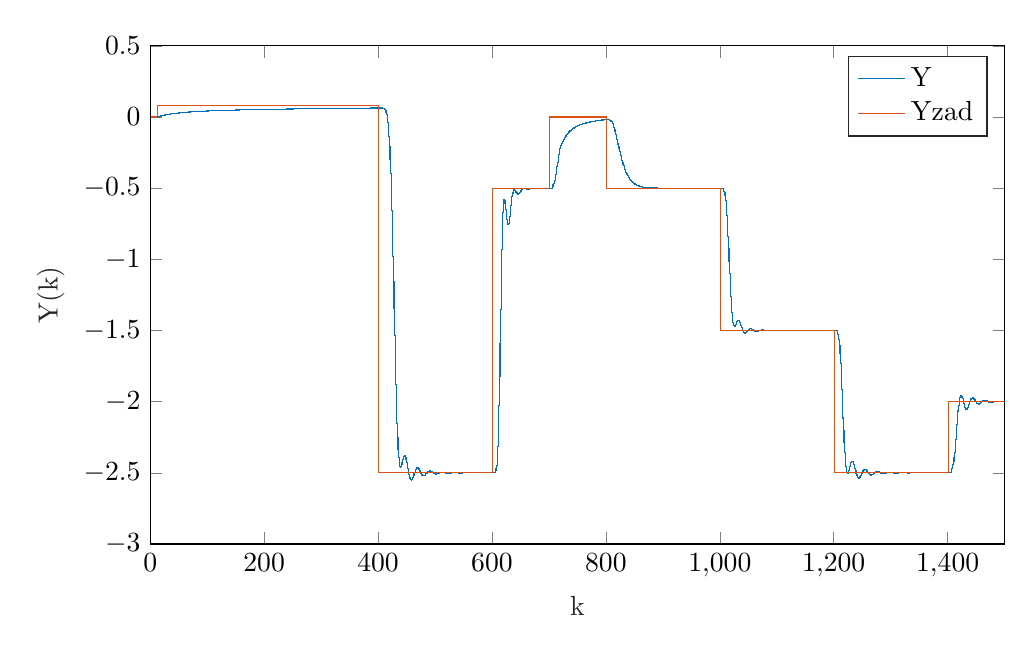
\begin{tikzpicture}

\begin{axis}[%
width=4.272in,
height=2.491in,
at={(0.717in,0.423in)},
scale only axis,
xmin=0,
xmax=1500,
xlabel style={font=\color{white!15!black}},
xlabel={k},
ymin=-3,
ymax=0.5,
ylabel style={font=\color{white!15!black}},
ylabel={Y(k)},
axis background/.style={fill=white},
legend style={legend cell align=left, align=left, draw=white!15!black}
]
\addplot[const plot, color=mycolor1] table[row sep=crcr] {%
1	0\\
2	0\\
3	0\\
4	0\\
5	0\\
6	0\\
7	0\\
8	0\\
9	0\\
10	0\\
11	0\\
12	0\\
13	0\\
14	0\\
15	0\\
16	0\\
17	0.00297346172952704\\
18	0.00704883380812825\\
19	0.00931929963074267\\
20	0.0106339270824205\\
21	0.0115309322119249\\
22	0.0122124506163222\\
23	0.0127334528163345\\
24	0.0132364392825915\\
25	0.0138305992750359\\
26	0.0145128206490361\\
27	0.015246786691758\\
28	0.0160005389056269\\
29	0.0167515353108469\\
30	0.0174832155030236\\
31	0.0181868124214139\\
32	0.0188613315519514\\
33	0.0195098532145398\\
34	0.0201363994170547\\
35	0.0207444814844265\\
36	0.0213366780823667\\
37	0.0219145864570644\\
38	0.0224790159797569\\
39	0.0230303162199029\\
40	0.0235686657760282\\
41	0.0240942444499011\\
42	0.0246073034813009\\
43	0.0251081743647332\\
44	0.0255972467781813\\
45	0.0260749368595626\\
46	0.0265416600114286\\
47	0.026997814112403\\
48	0.0274437725784818\\
49	0.0278798840203052\\
50	0.028306475201972\\
51	0.0287238548998101\\
52	0.0291323172730108\\
53	0.0295321442219258\\
54	0.0299236067778113\\
55	0.0303069658169365\\
56	0.0306824724154793\\
57	0.0310503680808225\\
58	0.0314108849926719\\
59	0.031764246303832\\
60	0.0321106664986447\\
61	0.0324503517848086\\
62	0.0327835004919437\\
63	0.0331103034574185\\
64	0.0334309443891395\\
65	0.0337456002023901\\
66	0.0340544413322236\\
67	0.034357632024715\\
68	0.0346553306104625\\
69	0.034947689763027\\
70	0.0352348567441368\\
71	0.0355169736368002\\
72	0.0357941775670408\\
73	0.0360666009147708\\
74	0.0363343715142641\\
75	0.0365976128446974\\
76	0.0368564442112578\\
77	0.0371109809173239\\
78	0.0373613344282254\\
79	0.0376076125270644\\
80	0.0378499194630518\\
81	0.0380883560927822\\
82	0.0383230200148379\\
83	0.038554005698087\\
84	0.0387814046040157\\
85	0.0390053053034116\\
86	0.0392257935876992\\
87	0.0394429525752071\\
88	0.0396568628126333\\
89	0.0398676023719576\\
90	0.0400752469430364\\
91	0.0402798699221009\\
92	0.0404815424963683\\
93	0.0406803337249621\\
94	0.0408763106163264\\
95	0.0410695382023104\\
96	0.0412600796090865\\
97	0.0414479961250598\\
98	0.041633347265914\\
99	0.0418161908369341\\
100	0.041996582992737\\
101	0.0421745782945344\\
102	0.0423502297650446\\
103	0.042523588941166\\
104	0.0426947059245161\\
105	0.0428636294299365\\
106	0.0430304068320576\\
107	0.0431950842100141\\
108	0.0433577063903932\\
109	0.0435183169884995\\
110	0.0436769584480095\\
111	0.0438336720790902\\
112	0.0439884980950506\\
113	0.044141475647589\\
114	0.0442926428607013\\
115	0.0444420368633065\\
116	0.0445896938206465\\
117	0.0447356489645137\\
118	0.0448799366223559\\
119	0.0450225902453076\\
120	0.0451636424351927\\
121	0.0453031249705432\\
122	0.0454410688316735\\
123	0.0455775042248525\\
124	0.0457124606056083\\
125	0.0458459667012036\\
126	0.0459780505323144\\
127	0.0461087394339458\\
128	0.046238060075615\\
129	0.046366038480832\\
130	0.0464927000459052\\
131	0.0466180695581002\\
132	0.0467421712131765\\
133	0.0468650286323276\\
134	0.0469866648785468\\
135	0.0471071024724425\\
136	0.0472263634075239\\
137	0.047344469164977\\
138	0.0474614407279518\\
139	0.0475772985953783\\
140	0.04769206279533\\
141	0.0478057528979514\\
142	0.0479183880279668\\
143	0.0480299868767855\\
144	0.0481405677142179\\
145	0.048250148399819\\
146	0.0483587463938708\\
147	0.0484663787680177\\
148	0.0485730622155681\\
149	0.0486788130614743\\
150	0.0487836472720008\\
151	0.0488875804640945\\
152	0.048990627914466\\
153	0.0490928045683924\\
154	0.0491941250482527\\
155	0.0492946036618028\\
156	0.0493942544102025\\
157	0.0494930909957999\\
158	0.0495911268296844\\
159	0.0496883750390141\\
160	0.0497848484741272\\
161	0.0498805597154432\\
162	0.0499755210801624\\
163	0.0500697446287698\\
164	0.0501632421713503\\
165	0.0502560252737209\\
166	0.0503481052633875\\
167	0.0504394932353306\\
168	0.0505302000576262\\
169	0.0506202363769073\\
170	0.050709612623672\\
171	0.0507983390174413\\
172	0.0508864255717737\\
173	0.0509738820991394\\
174	0.0510607182156603\\
175	0.0511469433457184\\
176	0.0512325667264384\\
177	0.0513175974120473\\
178	0.0514020442781154\\
179	0.0514859160256825\\
180	0.0515692211852732\\
181	0.0516519681208033\\
182	0.051734165033383\\
183	0.0518158199650178\\
184	0.0518969408022124\\
185	0.0519775352794782\\
186	0.0520576109827497\\
187	0.0521371753527112\\
188	0.0522162356880364\\
189	0.0522947991485445\\
190	0.0523728727582745\\
191	0.0524504634084805\\
192	0.0525275778605501\\
193	0.0526042227488487\\
194	0.052680404583491\\
195	0.0527561297530427\\
196	0.0528314045271543\\
197	0.0529062350591282\\
198	0.0529806273884225\\
199	0.0530545874430911\\
200	0.0531281210421652\\
201	0.0532012338979741\\
202	0.0532739316184099\\
203	0.0533462197091368\\
204	0.0534181035757458\\
205	0.053489588525858\\
206	0.0535606797711754\\
207	0.0536313824294841\\
208	0.0537017015266081\\
209	0.0537716419983165\\
210	0.0538412086921855\\
211	0.053910406369416\\
212	0.0539792397066082\\
213	0.0540477132974944\\
214	0.0541158316546308\\
215	0.0541835992110502\\
216	0.0542510203218756\\
217	0.0543180992658967\\
218	0.0543848402471097\\
219	0.0544512473962215\\
220	0.0545173247721197\\
221	0.0545830763633085\\
222	0.0546485060893119\\
223	0.0547136178020454\\
224	0.0547784152871557\\
225	0.0548429022653313\\
226	0.0549070823935827\\
227	0.0549709592664941\\
228	0.0550345364174474\\
229	0.0550978173198188\\
230	0.0551608053881482\\
231	0.0552235039792842\\
232	0.0552859163935021\\
233	0.0553480458755984\\
234	0.0554098956159612\\
235	0.0554714687516171\\
236	0.0555327683672548\\
237	0.0555937974962277\\
238	0.0556545591215335\\
239	0.0557150561767736\\
240	0.0557752915470914\\
241	0.0558352680700906\\
242	0.0558949885367341\\
243	0.0559544556922236\\
244	0.0560136722368603\\
245	0.0560726408268876\\
246	0.0561313640753165\\
247	0.0561898445527325\\
248	0.0562480847880868\\
249	0.0563060872694703\\
250	0.0563638544448711\\
251	0.0564213887229173\\
252	0.0564786924736038\\
253	0.0565357680290038\\
254	0.056592617683966\\
255	0.0566492436967979\\
256	0.0567056482899339\\
257	0.0567618336505913\\
258	0.0568178019314115\\
259	0.056873555251089\\
260	0.0569290956949877\\
261	0.0569844253157441\\
262	0.0570395461338591\\
263	0.0570944601382775\\
264	0.0571491692869557\\
265	0.0572036755074188\\
266	0.0572579806973055\\
267	0.0573120867249034\\
268	0.0573659954296726\\
269	0.0574197086227596\\
270	0.0574732280875009\\
271	0.0575265555799165\\
272	0.0575796928291942\\
273	0.0576326415381635\\
274	0.0576854033837616\\
275	0.057737980017489\\
276	0.057790373065857\\
277	0.0578425841308263\\
278	0.0578946147902373\\
279	0.0579464665982317\\
280	0.0579981410856666\\
281	0.0580496397605197\\
282	0.0581009641082881\\
283	0.058152115592378\\
284	0.0582030956544881\\
285	0.0582539057149853\\
286	0.0583045471732728\\
287	0.0583550214081523\\
288	0.0584053297781782\\
289	0.0584554736220061\\
290	0.0585054542587338\\
291	0.0585552729882371\\
292	0.0586049310914978\\
293	0.0586544298309272\\
294	0.058703770450682\\
295	0.0587529541769756\\
296	0.0588019822183828\\
297	0.0588508557661393\\
298	0.0588995759944355\\
299	0.0589481440607047\\
300	0.0589965611059064\\
301	0.0590448282548039\\
302	0.0590929466162374\\
303	0.0591409172833914\\
304	0.059188741334058\\
305	0.0592364198308945\\
306	0.0592839538216771\\
307	0.0593313443395496\\
308	0.0593785924032678\\
309	0.059425699017439\\
310	0.0594726651727578\\
311	0.0595194918462373\\
312	0.0595661800014362\\
313	0.0596127305886816\\
314	0.0596591445452885\\
315	0.0597054227957743\\
316	0.0597515662520707\\
317	0.0597975758137304\\
318	0.0598434523681316\\
319	0.0598891967906778\\
320	0.0599348099449944\\
321	0.059980292683122\\
322	0.060025645845706\\
323	0.0600708702621826\\
324	0.0601159667509627\\
325	0.0601609361196108\\
326	0.0602057791650225\\
327	0.0602504966735975\\
328	0.0602950894214101\\
329	0.0603395581743775\\
330	0.0603839036884235\\
331	0.0604281267096407\\
332	0.0604722279744496\\
333	0.0605162082097544\\
334	0.0605600681330966\\
335	0.0606038084528058\\
336	0.0606474298681481\\
337	0.0606909330694712\\
338	0.0607343187383481\\
339	0.0607775875477173\\
340	0.0608207401620213\\
341	0.0608637772373423\\
342	0.0609066994215357\\
343	0.0609495073543615\\
344	0.0609922016676128\\
345	0.0610347829852434\\
346	0.0610772519234915\\
347	0.0611196090910027\\
348	0.0611618550889505\\
349	0.0612039905111542\\
350	0.0612460159441954\\
351	0.0612879319675326\\
352	0.0613297391536135\\
353	0.0613714380679851\\
354	0.0614130292694031\\
355	0.061454513309938\\
356	0.0614958907350808\\
357	0.0615371620838456\\
358	0.0615783278888715\\
359	0.0616193886765221\\
360	0.0616603449669842\\
361	0.0617011972743636\\
362	0.0617419461067802\\
363	0.0617825919664617\\
364	0.0618231353498346\\
365	0.061863576747615\\
366	0.0619039166448968\\
367	0.0619441555212392\\
368	0.0619842938507527\\
369	0.0620243321021826\\
370	0.0620642707389929\\
371	0.0621041102194471\\
372	0.0621438509966889\\
373	0.0621834935188209\\
374	0.0622230382289821\\
375	0.062262485565424\\
376	0.0623018359615864\\
377	0.0623410898461701\\
378	0.0623802476432106\\
379	0.0624193097721484\\
380	0.0624582766479\\
381	0.0624971486809269\\
382	0.0625359262773028\\
383	0.0625746098387815\\
384	0.0626131997628615\\
385	0.0626516964428516\\
386	0.0626901002679338\\
387	0.0627284116232263\\
388	0.0627666308898446\\
389	0.0628047584449624\\
390	0.062842794661871\\
391	0.0628807399100377\\
392	0.0629185945551636\\
393	0.0629563589592403\\
394	0.0629940334806055\\
395	0.063031618473998\\
396	0.0630691142906114\\
397	0.0631065212781476\\
398	0.0631438397808687\\
399	0.0631810701396483\\
400	0.0632182126920226\\
401	0.0632552677722394\\
402	0.0632922357113076\\
403	0.0633291168370449\\
404	0.0633659114741257\\
405	0.0634026199441272\\
406	0.0633812354839849\\
407	0.0621345886526087\\
408	0.0623645151059485\\
409	0.0614667932025711\\
410	0.0593053013520207\\
411	0.0559586889214165\\
412	0.0511643579543011\\
413	0.0441820302667172\\
414	0.0337708675121055\\
415	0.0182366448023235\\
416	-0.00444443321953431\\
417	-0.0364374556797547\\
418	-0.0798375276711271\\
419	-0.136487249802122\\
420	-0.207860648969553\\
421	-0.295024722091382\\
422	-0.398665925202396\\
423	-0.51915622029187\\
424	-0.656631971602796\\
425	-0.810517675462165\\
426	-0.978899647873647\\
427	-1.15862677940365\\
428	-1.34564047416941\\
429	-1.53308230782877\\
430	-1.71233600252724\\
431	-1.8770644579624\\
432	-2.02386862417461\\
433	-2.15034046002176\\
434	-2.25463870870198\\
435	-2.33611556332224\\
436	-2.39541991008264\\
437	-2.43417023922192\\
438	-2.45478579801386\\
439	-2.46041228545204\\
440	-2.45470753084575\\
441	-2.44152839563146\\
442	-2.42463869301077\\
443	-2.40745803360194\\
444	-2.39284490084753\\
445	-2.38293937601274\\
446	-2.37908759420307\\
447	-2.3818434479785\\
448	-2.39103214426468\\
449	-2.40586155674299\\
450	-2.4250668760998\\
451	-2.44707260842866\\
452	-2.47015756730463\\
453	-2.49261169673282\\
454	-2.51287595483522\\
455	-2.52965811926983\\
456	-2.54201900198533\\
457	-2.54942529020999\\
458	-2.55176703523727\\
459	-2.54933991116407\\
460	-2.54279489430827\\
461	-2.53306076384659\\
462	-2.52124735815916\\
463	-2.50853935035093\\
464	-2.49609101682124\\
465	-2.48493185678174\\
466	-2.47589107274509\\
467	-2.46954621653496\\
468	-2.4661982625973\\
469	-2.46587249405786\\
470	-2.46834224483275\\
471	-2.47317091640719\\
472	-2.47976679522712\\
473	-2.48744493655903\\
474	-2.49549060322091\\
475	-2.50321930337788\\
476	-2.5100292419181\\
477	-2.51544290647438\\
478	-2.51913550785722\\
479	-2.52094905950988\\
480	-2.5208919841738\\
481	-2.51912523326093\\
482	-2.51593692559727\\
483	-2.51170836727486\\
484	-2.50687490952667\\
485	-2.50188536199569\\
486	-2.49716357019286\\
487	-2.49307530687118\\
488	-2.48990288738311\\
489	-2.48782900538773\\
490	-2.48693031818976\\
491	-2.48718040236862\\
492	-2.48846093626727\\
493	-2.49057939878941\\
494	-2.49329122340169\\
495	-2.49632420574437\\
496	-2.49940300930852\\
497	-2.50227181422857\\
498	-2.50471347494882\\
499	-2.50656395966468\\
500	-2.50772130570431\\
501	-2.50814880869343\\
502	-2.50787263738799\\
503	-2.50697449807626\\
504	-2.50558033121444\\
505	-2.50384628135699\\
506	-2.50194332018866\\
507	-2.50004191346494\\
508	-2.49829801093174\\
509	-2.49684142168231\\
510	-2.495767344107\\
511	-2.49513148391273\\
512	-2.49494885117018\\
513	-2.49519601022135\\
514	-2.49581629014851\\
515	-2.49672726557558\\
516	-2.49782969641321\\
517	-2.49901707158884\\
518	-2.50018493040223\\
519	-2.5012392259331\\
520	-2.50210313487064\\
521	-2.50272189238757\\
522	-2.50306542353293\\
523	-2.50312873830511\\
524	-2.50293024105287\\
525	-2.50250826268107\\
526	-2.50191624533282\\
527	-2.50121708615776\\
528	-2.50047717585352\\
529	-2.4997606496185\\
530	-2.49912430789414\\
531	-2.49861357025122\\
532	-2.49825970891907\\
533	-2.49807848089162\\
534	-2.49807015125798\\
535	-2.49822078608608\\
536	-2.4985045993505\\
537	-2.49888707086775\\
538	-2.49932851396595\\
539	-2.49978776293651\\
540	-2.5002256690823\\
541	-2.50060813636419\\
542	-2.50090848783355\\
543	-2.50110902593183\\
544	-2.50120172669499\\
545	-2.50118808341317\\
546	-2.50107818344611\\
547	-2.50088915775527\\
548	-2.50064318267419\\
549	-2.50036523542929\\
550	-2.50008080850466\\
551	-2.49981377425891\\
552	-2.49958456277529\\
553	-2.49940877634981\\
554	-2.49929631755536\\
555	-2.49925105894721\\
556	-2.49927103549454\\
557	-2.49934909947538\\
558	-2.49947394478073\\
559	-2.49963138527119\\
560	-2.49980576090369\\
561	-2.49998134567598\\
562	-2.50014364200248\\
563	-2.50028046519268\\
564	-2.50038274698286\\
565	-2.50044501600598\\
566	-2.50046554302926\\
567	-2.50044616723316\\
568	-2.50039184456182\\
569	-2.50030997852304\\
570	-2.50020960661244\\
571	-2.50010052126195\\
572	-2.4999924029743\\
573	-2.49989403577715\\
574	-2.499812662457\\
575	-2.49975352069407\\
576	-2.49971958287543\\
577	-2.49971150370359\\
578	-2.49972776230788\\
579	-2.49976497073459\\
580	-2.49981830943546\\
581	-2.49988204330775\\
582	-2.49995006917958\\
583	-2.50001644722014\\
584	-2.50007587409199\\
585	-2.50012406399678\\
586	-2.50015801416372\\
587	-2.50017614276924\\
588	-2.50017829873625\\
589	-2.50016565340565\\
590	-2.50014049291362\\
591	-2.50010593666624\\
592	-2.50006561122758\\
593	-2.50002331012843\\
594	-2.49998266868834\\
595	-2.49994687925925\\
596	-2.49991846683786\\
597	-2.49989913835526\\
598	-2.49988971178159\\
599	-2.49989012411639\\
600	-2.49989951094259\\
601	-2.4999163449729\\
602	-2.49993861724355\\
603	-2.49996404249728\\
604	-2.49999026987522\\
605	-2.50001508119842\\
606	-2.48497352228894\\
607	-2.47124473722381\\
608	-2.4489190842847\\
609	-2.40131517100267\\
610	-2.31797895688067\\
611	-2.19400983306228\\
612	-2.02819898875246\\
613	-1.8235600177043\\
614	-1.59223103960372\\
615	-1.35318074444532\\
616	-1.12695766295961\\
617	-0.930957875622019\\
618	-0.776608379925952\\
619	-0.668379465949329\\
620	-0.604742095731326\\
621	-0.579910447662062\\
622	-0.585494838020323\\
623	-0.611855099802369\\
624	-0.649229895635519\\
625	-0.688652156743527\\
626	-0.722638389850858\\
627	-0.745678822008643\\
628	-0.754547025728791\\
629	-0.748398519944705\\
630	-0.7286062343311\\
631	-0.69831234862784\\
632	-0.661745445049646\\
633	-0.623429273157607\\
634	-0.587451616602594\\
635	-0.556936145768695\\
636	-0.533780962331172\\
637	-0.518644850925203\\
638	-0.511114369510635\\
639	-0.509975120391174\\
640	-0.513522062668218\\
641	-0.519861135927268\\
642	-0.527170533303257\\
643	-0.533902651683016\\
644	-0.538917160624032\\
645	-0.541542911383613\\
646	-0.541572875972734\\
647	-0.53920253928549\\
648	-0.534927671611227\\
649	-0.529421018333593\\
650	-0.52340805683054\\
651	-0.517559235183466\\
652	-0.51241071532289\\
653	-0.508319060945317\\
654	-0.505449132405664\\
655	-0.503789810257144\\
656	-0.503189508256863\\
657	-0.503402623132191\\
658	-0.504138662341625\\
659	-0.505107283308609\\
660	-0.506054425844292\\
661	-0.506786790355119\\
662	-0.507183871064407\\
663	-0.507198426872299\\
664	-0.506847541592209\\
665	-0.506197213802091\\
666	-0.505343701075335\\
667	-0.504394661610228\\
668	-0.503452584482079\\
669	-0.50260221568668\\
670	-0.501902822902411\\
671	-0.50138533511954\\
672	-0.501053745702804\\
673	-0.500889735186482\\
674	-0.50085926533858\\
675	-0.50091989636059\\
676	-0.501027739899591\\
677	-0.50114322693963\\
678	-0.5012351859661\\
679	-0.50128304340667\\
680	-0.501277235822875\\
681	-0.501218134730438\\
682	-0.501113916494481\\
683	-0.50097786013951\\
684	-0.500825534269868\\
685	-0.500672257300418\\
686	-0.50053110361132\\
687	-0.500411603409454\\
688	-0.500319164939863\\
689	-0.500255148669411\\
690	-0.500217453023619\\
691	-0.500201433444244\\
692	-0.50020096932249\\
693	-0.500209511488238\\
694	-0.50022097894875\\
695	-0.500230419245174\\
696	-0.500234394336809\\
697	-0.500231096865422\\
698	-0.50022023540634\\
699	-0.500202749375893\\
700	-0.50018042412394\\
701	-0.500155475551013\\
702	-0.500130163700366\\
703	-0.500106479191593\\
704	-0.500085928229653\\
705	-0.500069424090264\\
706	-0.486003009190685\\
707	-0.475132392115114\\
708	-0.467745197530905\\
709	-0.4581653076448\\
710	-0.443391865087971\\
711	-0.424512658846541\\
712	-0.401707332879954\\
713	-0.375089297263763\\
714	-0.346057684893486\\
715	-0.316702650874204\\
716	-0.288770913595475\\
717	-0.263513534474616\\
718	-0.241737467107398\\
719	-0.223720571780889\\
720	-0.209216345739703\\
721	-0.197627410454615\\
722	-0.188205098332122\\
723	-0.180197829250868\\
724	-0.172960049038456\\
725	-0.166024743769899\\
726	-0.159126631610033\\
727	-0.152180093860602\\
728	-0.145230879099382\\
729	-0.138399101488875\\
730	-0.131825800678983\\
731	-0.12563202625228\\
732	-0.119895161009372\\
733	-0.114642017774214\\
734	-0.10985466475165\\
735	-0.105483687043676\\
736	-0.101463853571653\\
737	-0.0977282475091369\\
738	-0.0942184627569978\\
739	-0.0908900527658908\\
740	-0.087713663279255\\
741	-0.0846730235169899\\
742	-0.0817612298040963\\
743	-0.0789766357256041\\
744	-0.0763193061263365\\
745	-0.0737885506834606\\
746	-0.0713816511173272\\
747	-0.0690936081292608\\
748	-0.066917582713552\\
749	-0.0648456769566247\\
750	-0.0628697558558746\\
751	-0.0609821117336887\\
752	-0.0591758793811679\\
753	-0.0574451977591451\\
754	-0.0557851707095408\\
755	-0.0541917036351506\\
756	-0.0526612918483612\\
757	-0.0511908189910934\\
758	-0.0497774003036865\\
759	-0.048418283110284\\
760	-0.0471108001726807\\
761	-0.045852362091982\\
762	-0.0446404720666926\\
763	-0.0434727481779185\\
764	-0.0423469427512243\\
765	-0.0412609533065319\\
766	-0.0402128238282146\\
767	-0.0392007379180613\\
768	-0.0382230067470064\\
769	-0.037278054875429\\
770	-0.036364406405213\\
771	-0.03548067299738\\
772	-0.0346255443749608\\
773	-0.0337977812326408\\
774	-0.0329962100646968\\
775	-0.0322197192788739\\
776	-0.0314672560124751\\
777	-0.0307378232201753\\
778	-0.0300304767845825\\
779	-0.0293443225583359\\
780	-0.0286785133549951\\
781	-0.0280322459611455\\
782	-0.0274047582537872\\
783	-0.0267953264908624\\
784	-0.0262032628142743\\
785	-0.0256279129758925\\
786	-0.0250686542748815\\
787	-0.0245248936817882\\
788	-0.0239960661205181\\
789	-0.0234816328812356\\
790	-0.0229810801424925\\
791	-0.0224939175870705\\
792	-0.0220196771014737\\
793	-0.021557911552916\\
794	-0.0211081936399018\\
795	-0.0206701148133957\\
796	-0.0202432842655905\\
797	-0.0198273279828938\\
798	-0.0194218878593023\\
799	-0.0190266208660414\\
800	-0.0186411982732851\\
801	-0.0182653049199212\\
802	-0.0178986385276284\\
803	-0.0175409090559026\\
804	-0.0171918380950452\\
805	-0.0168511582944685\\
806	-0.0214406872521675\\
807	-0.0251131719500729\\
808	-0.0260472486872006\\
809	-0.0279607142405433\\
810	-0.0323291424286814\\
811	-0.0391694997071999\\
812	-0.0482798247848943\\
813	-0.0596729987043159\\
814	-0.0730819003661665\\
815	-0.0880148896712089\\
816	-0.104021633047809\\
817	-0.120756680066818\\
818	-0.137932470089574\\
819	-0.155311069673711\\
820	-0.1727194750304\\
821	-0.190038598333174\\
822	-0.207179942518058\\
823	-0.224071445515066\\
824	-0.240650713477549\\
825	-0.256859062787474\\
826	-0.272637403131689\\
827	-0.287925864921643\\
828	-0.302665864953391\\
829	-0.31680283123464\\
830	-0.330289020483432\\
831	-0.343086173905768\\
832	-0.355167527424798\\
833	-0.366518832410218\\
834	-0.377138370262997\\
835	-0.387036096950314\\
836	-0.396232089871308\\
837	-0.404754517394797\\
838	-0.412637387528955\\
839	-0.41991831504557\\
840	-0.426636495855808\\
841	-0.432831021113194\\
842	-0.438539606184268\\
843	-0.443797752579257\\
844	-0.448638311991177\\
845	-0.453091386891321\\
846	-0.457184482309298\\
847	-0.460942816984445\\
848	-0.464389707226133\\
849	-0.467546950850742\\
850	-0.470435157890569\\
851	-0.473073995896897\\
852	-0.475482337731218\\
853	-0.477678316614891\\
854	-0.479679305516948\\
855	-0.481501845165373\\
856	-0.483161547285979\\
857	-0.484672997877507\\
858	-0.48604968053685\\
859	-0.487303933313226\\
860	-0.488446945514563\\
861	-0.489488794346055\\
862	-0.490438515982742\\
863	-0.491304202100999\\
864	-0.492093111146622\\
865	-0.49281178356654\\
866	-0.493466151551968\\
867	-0.494061636096692\\
868	-0.494603226895482\\
869	-0.495095543358263\\
870	-0.495542877442089\\
871	-0.495949220862744\\
872	-0.496318280418874\\
873	-0.49665348563355\\
874	-0.496957992771772\\
875	-0.49723468867091\\
876	-0.497486196899555\\
877	-0.49771488771702\\
878	-0.497922892298682\\
879	-0.498112120843209\\
880	-0.498284283563121\\
881	-0.498440913211535\\
882	-0.498583387706018\\
883	-0.498712951534932\\
884	-0.498830734912294\\
885	-0.49893777001601\\
886	-0.499035004035328\\
887	-0.499123309111212\\
888	-0.499203489537771\\
889	-0.499276286781427\\
890	-0.499342382961335\\
891	-0.499402403428316\\
892	-0.499456918999012\\
893	-0.499506448271871\\
894	-0.499551460298036\\
895	-0.499592377727262\\
896	-0.499629580415769\\
897	-0.499663409382254\\
898	-0.499694170936287\\
899	-0.499722140779839\\
900	-0.499747567892846\\
901	-0.499770678049133\\
902	-0.499791676859851\\
903	-0.49981075229797\\
904	-0.499828076710735\\
905	-0.499843808370823\\
906	-0.499858092647375\\
907	-0.499871062893677\\
908	-0.499882841149794\\
909	-0.499893538748507\\
910	-0.499903256894743\\
911	-0.499912087266408\\
912	-0.499920112661463\\
913	-0.499927407695514\\
914	-0.499934039537963\\
915	-0.499940068664183\\
916	-0.499945549596324\\
917	-0.499950531605654\\
918	-0.499955059353686\\
919	-0.499959173456288\\
920	-0.499962910963082\\
921	-0.49996630575235\\
922	-0.499969388848387\\
923	-0.49997218867313\\
924	-0.499974731246576\\
925	-0.499977040351117\\
926	-0.499979137673755\\
927	-0.49998104293764\\
928	-0.499982774031193\\
929	-0.499984347139576\\
930	-0.499985776880157\\
931	-0.499987076440998\\
932	-0.499988257719629\\
933	-0.499989331458467\\
934	-0.499990307373055\\
935	-0.499991194269832\\
936	-0.499992000151059\\
937	-0.499992732305678\\
938	-0.499993397386053\\
939	-0.499994001471549\\
940	-0.499994550120705\\
941	-0.499995048414161\\
942	-0.49999550099071\\
943	-0.499995912078658\\
944	-0.499996285524364\\
945	-0.499996624819382\\
946	-0.49999693312707\\
947	-0.499997213309096\\
948	-0.499997467951825\\
949	-0.499997699392291\\
950	-0.499997909743296\\
951	-0.499998100917115\\
952	-0.499998274647342\\
953	-0.49999843250853\\
954	-0.499998575933453\\
955	-0.499998706227959\\
956	-0.499998824583566\\
957	-0.499998932088061\\
958	-0.499999029734421\\
959	-0.499999118428441\\
960	-0.499999198995405\\
961	-0.499999272186113\\
962	-0.499999338682492\\
963	-0.49999939910297\\
964	-0.499999454007689\\
965	-0.499999503903584\\
966	-0.499999549249304\\
967	-0.499999590459924\\
968	-0.499999627911375\\
969	-0.499999661944538\\
970	-0.499999692868944\\
971	-0.499999720966064\\
972	-0.499999746492179\\
973	-0.499999769680861\\
974	-0.499999790745095\\
975	-0.499999809879103\\
976	-0.499999827259916\\
977	-0.499999843048762\\
978	-0.499999857392313\\
979	-0.499999870423838\\
980	-0.499999882264274\\
981	-0.499999893023264\\
982	-0.499999902800136\\
983	-0.499999911684848\\
984	-0.49999991975888\\
985	-0.49999992709607\\
986	-0.49999993376339\\
987	-0.499999939821645\\
988	-0.499999945326103\\
989	-0.499999950327051\\
990	-0.499999954870281\\
991	-0.499999958997509\\
992	-0.499999962746745\\
993	-0.499999966152613\\
994	-0.499999969246635\\
995	-0.499999972057481\\
996	-0.49999997461121\\
997	-0.499999976931481\\
998	-0.499999979039754\\
999	-0.49999998095549\\
1000	-0.499999982696325\\
1001	-0.499999984278244\\
1002	-0.499999985715741\\
1003	-0.499999987021965\\
1004	-0.499999988208854\\
1005	-0.499999989287256\\
1006	-0.512415430242033\\
1007	-0.522500161900245\\
1008	-0.53355783271318\\
1009	-0.553731155790376\\
1010	-0.586950390369599\\
1011	-0.633011363591918\\
1012	-0.691572452687167\\
1013	-0.761828915214594\\
1014	-0.841430275725767\\
1015	-0.926978664537427\\
1016	-1.01486574440313\\
1017	-1.10154555617271\\
1018	-1.18361962283096\\
1019	-1.25808636460383\\
1020	-1.32259819387368\\
1021	-1.37558861217883\\
1022	-1.41631812575177\\
1023	-1.4448859567586\\
1024	-1.46218262922115\\
1025	-1.46976572061394\\
1026	-1.46967783333293\\
1027	-1.46423296539246\\
1028	-1.4557922014257\\
1029	-1.44655228589265\\
1030	-1.4383717736725\\
1031	-1.43265153362277\\
1032	-1.43027532428119\\
1033	-1.43160763421004\\
1034	-1.43654018217949\\
1035	-1.44457478073028\\
1036	-1.45492893162464\\
1037	-1.46665122915605\\
1038	-1.47873540337422\\
1039	-1.49022389967661\\
1040	-1.50029401434041\\
1041	-1.5083217182517\\
1042	-1.513920370168\\
1043	-1.5169535665773\\
1044	-1.5175234191122\\
1045	-1.51593752482529\\
1046	-1.51265962433511\\
1047	-1.50825019852112\\
1048	-1.50330382800387\\
1049	-1.49838991748214\\
1050	-1.49400240077982\\
1051	-1.49052247248721\\
1052	-1.48819651794275\\
1053	-1.4871295361537\\
1054	-1.48729272137717\\
1055	-1.48854264798018\\
1056	-1.49064875056631\\
1057	-1.49332548827121\\
1058	-1.4962656607651\\
1059	-1.49917171630917\\
1060	-1.50178247208302\\
1061	-1.50389337682397\\
1062	-1.50536921967946\\
1063	-1.50614896904157\\
1064	-1.50624315699827\\
1065	-1.5057248574451\\
1066	-1.50471579219305\\
1067	-1.50336940315039\\
1068	-1.50185283023344\\
1069	-1.50032963633228\\
1070	-1.49894484779275\\
1071	-1.49781347645012\\
1072	-1.49701321434504\\
1073	-1.49658150462577\\
1074	-1.49651674531977\\
1075	-1.49678301751337\\
1076	-1.49731747116423\\
1077	-1.49803935982708\\
1078	-1.49885968626315\\
1079	-1.49969049061413\\
1080	-1.50045296155886\\
1081	-1.50108375524608\\
1082	-1.50153914233789\\
1083	-1.50179684637421\\
1084	-1.50185566506453\\
1085	-1.50173316144136\\
1086	-1.50146185982414\\
1087	-1.50108447328049\\
1088	-1.50064872164425\\
1089	-1.50020227498803\\
1090	-1.49978828490083\\
1091	-1.49944185723296\\
1092	-1.49918768980035\\
1093	-1.49903896211694\\
1094	-1.4989974356048\\
1095	-1.49905461343314\\
1096	-1.49919372726333\\
1097	-1.4993922680821\\
1098	-1.49962476072565\\
1099	-1.49986549422703\\
1100	-1.50009095790294\\
1101	-1.50028178961375\\
1102	-1.5004241104889\\
1103	-1.50051019208576\\
1104	-1.50053847043946\\
1105	-1.50051298082219\\
1106	-1.50044233278977\\
1107	-1.50033837449727\\
1108	-1.50021470737027\\
1109	-1.50008520780479\\
1110	-1.49996269389815\\
1111	-1.49985784566491\\
1112	-1.49977845081182\\
1113	-1.49972900917664\\
1114	-1.49971069137764\\
1115	-1.49972161446484\\
1116	-1.49975737193958\\
1117	-1.49981173894155\\
1118	-1.49987746619946\\
1119	-1.49994707806988\\
1120	-1.50001359943408\\
1121	-1.50007115160057\\
1122	-1.50011537654624\\
1123	-1.5001436695959\\
1124	-1.50015522087032\\
1125	-1.50015088370421\\
1126	-1.5001329023478\\
1127	-1.50010454073034\\
1128	-1.50006965852355\\
1129	-1.50003228035224\\
1130	-1.49999619934963\\
1131	-1.49996464827241\\
1132	-1.49994006120992\\
1133	-1.49992393775546\\
1134	-1.49991681051949\\
1135	-1.49991830706847\\
1136	-1.49992728954975\\
1137	-1.49994204991839\\
1138	-1.4999605360279\\
1139	-1.49998058381978\\
1140	-1.50000013314234\\
1141	-1.50001740886474\\
1142	-1.50003105432476\\
1143	-1.50004021011461\\
1144	-1.50004453714062\\
1145	-1.50004418823778\\
1146	-1.50003973694809\\
1147	-1.50003207509204\\
1148	-1.50002229234479\\
1149	-1.50001155118872\\
1150	-1.50000096950215\\
1151	-1.49999152091023\\
1152	-1.49998396018726\\
1153	-1.4999787778073\\
1154	-1.4999761845324\\
1155	-1.49997612400843\\
1156	-1.49997830894703\\
1157	-1.49998227477281\\
1158	-1.49998744368541\\
1159	-1.49999319192608\\
1160	-1.49999891357181\\
1161	-1.50000407527831\\
1162	-1.50000825788685\\
1163	-1.50001118251387\\
1164	-1.5000127204721\\
1165	-1.50001288796313\\
1166	-1.50001182780018\\
1167	-1.50000978137455\\
1168	-1.50000705462239\\
1169	-1.50000398187643\\
1170	-1.50000089123639\\
1171	-1.49999807452931\\
1172	-1.49999576414513\\
1173	-1.49999411812429\\
1174	-1.49999321394072\\
1175	-1.49999305055753\\
1176	-1.4999935576055\\
1177	-1.49999461\\
1178	-1.49999604599691\\
1179	-1.49999768659688\\
1180	-1.49999935432288\\
1181	-1.50000088968301\\
1182	-1.50000216404299\\
1183	-1.50000308811677\\
1184	-1.50000361578609\\
1185	-1.50000374343111\\
1186	-1.50000350535423\\
1187	-1.50000296617774\\
1188	-1.50000221127835\\
1189	-1.50000133638221\\
1190	-1.50000043739321\\
1191	-1.49999960138109\\
1192	-1.49999889944017\\
1193	-1.49999838187193\\
1194	-1.49999807587405\\
1195	-1.49999798566297\\
1196	-1.49999809473675\\
1197	-1.49999836981864\\
1198	-1.49999876591715\\
1199	-1.49999923189919\\
1200	-1.49999971599428\\
1201	-1.50000017072196\\
1202	-1.50000055684698\\
1203	-1.500000846104\\
1204	-1.50000102257872\\
1205	-1.50000108277131\\
1206	-1.51370142474681\\
1207	-1.52606199310926\\
1208	-1.54031353222568\\
1209	-1.56525081814264\\
1210	-1.60564291695549\\
1211	-1.66170783982643\\
1212	-1.7332800929341\\
1213	-1.81949627730988\\
1214	-1.91657469504574\\
1215	-2.01713646370962\\
1216	-2.11482914500099\\
1217	-2.20564718406335\\
1218	-2.28692468686062\\
1219	-2.35628766481278\\
1220	-2.41212602748039\\
1221	-2.45390680671754\\
1222	-2.48197334541529\\
1223	-2.49734637097401\\
1224	-2.50168402703281\\
1225	-2.4971795987095\\
1226	-2.48634757647072\\
1227	-2.47179926753431\\
1228	-2.45604904012338\\
1229	-2.44133797977431\\
1230	-2.42948462167057\\
1231	-2.42178684100998\\
1232	-2.41898147406869\\
1233	-2.42125414665146\\
1234	-2.42829098783634\\
1235	-2.43936389188167\\
1236	-2.45343841020174\\
1237	-2.46929259060025\\
1238	-2.48563675207411\\
1239	-2.50122602682371\\
1240	-2.51495881015041\\
1241	-2.52595560983921\\
1242	-2.53361435304885\\
1243	-2.53763980647671\\
1244	-2.5380464151171\\
1245	-2.5351356915641\\
1246	-2.52945123636719\\
1247	-2.52171631163691\\
1248	-2.51276035281774\\
1249	-2.5034416396945\\
1250	-2.49457338400875\\
1251	-2.48685969518669\\
1252	-2.48084639459388\\
1253	-2.47688972742881\\
1254	-2.47514398240692\\
1255	-2.47556715514352\\
1256	-2.4779422815031\\
1257	-2.48191102034105\\
1258	-2.48701548854073\\
1259	-2.49274419108962\\
1260	-2.49857806245687\\
1261	-2.50403305742991\\
1262	-2.5086963273207\\
1263	-2.51225373604147\\
1264	-2.51450726879686\\
1265	-2.51538172831144\\
1266	-2.51492096034008\\
1267	-2.51327465306903\\
1268	-2.51067745585046\\
1269	-2.50742270032491\\
1270	-2.50383332812708\\
1271	-2.50023270107616\\
1272	-2.49691778869015\\
1273	-2.49413682328112\\
1274	-2.49207294201722\\
1275	-2.49083467269497\\
1276	-2.49045344389083\\
1277	-2.49088768036\\
1278	-2.49203253350542\\
1279	-2.49373392610906\\
1280	-2.49580537204173\\
1281	-2.49804596102431\\
1282	-2.5002579603249\\
1283	-2.5022626577494\\
1284	-2.50391332862206\\
1285	-2.50510452782281\\
1286	-2.50577726028183\\
1287	-2.50591994358896\\
1288	-2.50556541887225\\
1289	-2.50478456639974\\
1290	-2.50367731885777\\
1291	-2.50236202127655\\
1292	-2.50096415244215\\
1293	-2.49960539719779\\
1294	-2.49839395003941\\
1295	-2.49741675355111\\
1296	-2.49673415201768\\
1297	-2.49637719540189\\
1298	-2.4963475860036\\
1299	-2.49662004086422\\
1300	-2.49714666390479\\
1301	-2.49786279371723\\
1302	-2.49869372088019\\
1303	-2.4995616524057\\
1304	-2.50039233588531\\
1305	-2.50112083427578\\
1306	-2.50169605397926\\
1307	-2.50208376251788\\
1308	-2.50226797571182\\
1309	-2.50225073605041\\
1310	-2.50205043298416\\
1311	-2.50169892281823\\
1312	-2.50123778362673\\
1313	-2.50071408474712\\
1314	-2.50017605962485\\
1315	-2.49966904681932\\
1316	-2.49923201141219\\
1317	-2.49889488465432\\
1318	-2.49867687164176\\
1319	-2.49858578383482\\
1320	-2.49861836367551\\
1321	-2.49876148966009\\
1322	-2.49899408758461\\
1323	-2.49928953095178\\
1324	-2.49961829233594\\
1325	-2.49995060756146\\
1326	-2.50025893391129\\
1327	-2.50052001896832\\
1328	-2.50071644388657\\
1329	-2.50083755912904\\
1330	-2.50087978708237\\
1331	-2.50084631977509\\
1332	-2.500746287051\\
1333	-2.5005935076846\\
1334	-2.50040496081919\\
1335	-2.50019912667532\\
1336	-2.4999943438152\\
1337	-2.49980731655931\\
1338	-2.49965188255471\\
1339	-2.49953811978249\\
1340	-2.4994718376264\\
1341	-2.49945446123266\\
1342	-2.49948328527596\\
1343	-2.49955204495144\\
1344	-2.49965173044588\\
1345	-2.49977155748229\\
1346	-2.49990000120124\\
1347	-2.5000258033461\\
1348	-2.50013887253907\\
1349	-2.50023101296223\\
1350	-2.50029643624648\\
1351	-2.50033203290748\\
1352	-2.50033740133145\\
1353	-2.50031465233225\\
1354	-2.50026802417761\\
1355	-2.50020335559633\\
1356	-2.50012747194415\\
1357	-2.50004754220226\\
1358	-2.49997046202993\\
1359	-2.49990231130377\\
1360	-2.49984792437393\\
1361	-2.49981059878087\\
1362	-2.49979195462865\\
1363	-2.49979194341051\\
1364	-2.49980899291989\\
1365	-2.49984026485054\\
1366	-2.49988199443317\\
1367	-2.49992987732935\\
1368	-2.49997946807738\\
1369	-2.50002655645969\\
1370	-2.50006749281288\\
1371	-2.50009943993092\\
1372	-2.5001205371101\\
1373	-2.50012997030017\\
1374	-2.50012795052785\\
1375	-2.50011561009408\\
1376	-2.50009483198747\\
1377	-2.50006803213204\\
1378	-2.50003791630416\\
1379	-2.50000723379169\\
1380	-2.49997854827509\\
1381	-2.49995404327008\\
1382	-2.4999353751718\\
1383	-2.4999235819341\\
1384	-2.49991905017425\\
1385	-2.49992153846527\\
1386	-2.49993025015863\\
1387	-2.49994394558174\\
1388	-2.49996108108478\\
1389	-2.49997996126908\\
1390	-2.49999889080413\\
1391	-2.50001631342231\\
1392	-2.5000309277792\\
1393	-2.5000417726344\\
1394	-2.50004827695864\\
1395	-2.50005027381894\\
1396	-2.50004797995943\\
1397	-2.50004194564633\\
1398	-2.50003298139821\\
1399	-2.50002206955989\\
1400	-2.50001026924984\\
1401	-2.49999862303498\\
1402	-2.49998807284016\\
1403	-2.49997939120876\\
1404	-2.49997313225535\\
1405	-2.49996960466989\\
1406	-2.48490401852365\\
1407	-2.47115560005613\\
1408	-2.45959411320107\\
1409	-2.44451560344753\\
1410	-2.4223274186876\\
1411	-2.39359926392982\\
1412	-2.3581997691172\\
1413	-2.31580340987542\\
1414	-2.26752796115401\\
1415	-2.21574381014284\\
1416	-2.16308414268568\\
1417	-2.11219638610142\\
1418	-2.06569332286727\\
1419	-2.02584935705341\\
1420	-1.99429167345508\\
1421	-1.97189951185663\\
1422	-1.95881820697855\\
1423	-1.95450528697023\\
1424	-1.95782555387084\\
1425	-1.96720146546474\\
1426	-1.98078615677861\\
1427	-1.99663302109788\\
1428	-2.0128540469095\\
1429	-2.02776056701827\\
1430	-2.03997677810283\\
1431	-2.04851907617949\\
1432	-2.05283849640195\\
1433	-2.05282554587849\\
1434	-2.04877846527455\\
1435	-2.04133897309313\\
1436	-2.03140280575428\\
1437	-2.02001475686538\\
1438	-2.00825919087666\\
1439	-1.99715701731825\\
1440	-1.98757869220467\\
1441	-1.98018017521019\\
1442	-1.97536550632755\\
1443	-1.97327641052709\\
1444	-1.97380656600834\\
1445	-1.97663615257761\\
1446	-1.98128111029679\\
1447	-1.98715110539631\\
1448	-1.99361035528157\\
1449	-2.0000360306512\\
1450	-2.0058697847608\\
1451	-2.01065895506542\\
1452	-2.0140850756303\\
1453	-2.01597848673381\\
1454	-2.0163189904526\\
1455	-2.0152236234358\\
1456	-2.01292362625204\\
1457	-2.00973349451046\\
1458	-2.00601551522227\\
1459	-2.00214336209524\\
1460	-1.99846812875659\\
1461	-1.99528965461346\\
1462	-1.99283522648618\\
1463	-1.99124683235508\\
1464	-1.99057722036131\\
1465	-1.99079418073923\\
1466	-1.99179179584965\\
1467	-1.99340693515825\\
1468	-1.99543901798175\\
1469	-1.99767101371711\\
1470	-1.99988976907353\\
1471	-2.00190400952582\\
1472	-2.00355872083498\\
1473	-2.00474503959955\\
1474	-2.00540523416574\\
1475	-2.00553280474587\\
1476	-2.00516814163415\\
1477	-2.00439052304075\\
1478	-2.00330748437917\\
1479	-2.00204273179065\\
1480	-2.00072379763138\\
1481	-1.9994705496965\\
1482	-1.99838548553426\\
1483	-1.99754649374129\\
1484	-1.99700247634628\\
1485	-1.99677193200547\\
1486	-1.99684432750462\\
1487	-1.99718385781661\\
1488	-1.99773502799647\\
1489	-1.99842939096885\\
1490	-1.99919274411748\\
1491	-1.99995211904576\\
1492	-2.00064198316481\\
1493	-2.00120919625689\\
1494	-2.00161641567067\\
1495	-2.00184380566101\\
1496	-2.00188906539208\\
1497	-2.00176593342924\\
1498	-2.00150144346285\\
1499	-2.00113228873841\\
1500	-2.00070069684102\\
};
\addlegendentry{Y}

\addplot[const plot, color=mycolor2] table[row sep=crcr] {%
1	0\\
2	0\\
3	0\\
4	0\\
5	0\\
6	0\\
7	0\\
8	0\\
9	0\\
10	0\\
11	0\\
12	0.08\\
13	0.08\\
14	0.08\\
15	0.08\\
16	0.08\\
17	0.08\\
18	0.08\\
19	0.08\\
20	0.08\\
21	0.08\\
22	0.08\\
23	0.08\\
24	0.08\\
25	0.08\\
26	0.08\\
27	0.08\\
28	0.08\\
29	0.08\\
30	0.08\\
31	0.08\\
32	0.08\\
33	0.08\\
34	0.08\\
35	0.08\\
36	0.08\\
37	0.08\\
38	0.08\\
39	0.08\\
40	0.08\\
41	0.08\\
42	0.08\\
43	0.08\\
44	0.08\\
45	0.08\\
46	0.08\\
47	0.08\\
48	0.08\\
49	0.08\\
50	0.08\\
51	0.08\\
52	0.08\\
53	0.08\\
54	0.08\\
55	0.08\\
56	0.08\\
57	0.08\\
58	0.08\\
59	0.08\\
60	0.08\\
61	0.08\\
62	0.08\\
63	0.08\\
64	0.08\\
65	0.08\\
66	0.08\\
67	0.08\\
68	0.08\\
69	0.08\\
70	0.08\\
71	0.08\\
72	0.08\\
73	0.08\\
74	0.08\\
75	0.08\\
76	0.08\\
77	0.08\\
78	0.08\\
79	0.08\\
80	0.08\\
81	0.08\\
82	0.08\\
83	0.08\\
84	0.08\\
85	0.08\\
86	0.08\\
87	0.08\\
88	0.08\\
89	0.08\\
90	0.08\\
91	0.08\\
92	0.08\\
93	0.08\\
94	0.08\\
95	0.08\\
96	0.08\\
97	0.08\\
98	0.08\\
99	0.08\\
100	0.08\\
101	0.08\\
102	0.08\\
103	0.08\\
104	0.08\\
105	0.08\\
106	0.08\\
107	0.08\\
108	0.08\\
109	0.08\\
110	0.08\\
111	0.08\\
112	0.08\\
113	0.08\\
114	0.08\\
115	0.08\\
116	0.08\\
117	0.08\\
118	0.08\\
119	0.08\\
120	0.08\\
121	0.08\\
122	0.08\\
123	0.08\\
124	0.08\\
125	0.08\\
126	0.08\\
127	0.08\\
128	0.08\\
129	0.08\\
130	0.08\\
131	0.08\\
132	0.08\\
133	0.08\\
134	0.08\\
135	0.08\\
136	0.08\\
137	0.08\\
138	0.08\\
139	0.08\\
140	0.08\\
141	0.08\\
142	0.08\\
143	0.08\\
144	0.08\\
145	0.08\\
146	0.08\\
147	0.08\\
148	0.08\\
149	0.08\\
150	0.08\\
151	0.08\\
152	0.08\\
153	0.08\\
154	0.08\\
155	0.08\\
156	0.08\\
157	0.08\\
158	0.08\\
159	0.08\\
160	0.08\\
161	0.08\\
162	0.08\\
163	0.08\\
164	0.08\\
165	0.08\\
166	0.08\\
167	0.08\\
168	0.08\\
169	0.08\\
170	0.08\\
171	0.08\\
172	0.08\\
173	0.08\\
174	0.08\\
175	0.08\\
176	0.08\\
177	0.08\\
178	0.08\\
179	0.08\\
180	0.08\\
181	0.08\\
182	0.08\\
183	0.08\\
184	0.08\\
185	0.08\\
186	0.08\\
187	0.08\\
188	0.08\\
189	0.08\\
190	0.08\\
191	0.08\\
192	0.08\\
193	0.08\\
194	0.08\\
195	0.08\\
196	0.08\\
197	0.08\\
198	0.08\\
199	0.08\\
200	0.08\\
201	0.08\\
202	0.08\\
203	0.08\\
204	0.08\\
205	0.08\\
206	0.08\\
207	0.08\\
208	0.08\\
209	0.08\\
210	0.08\\
211	0.08\\
212	0.08\\
213	0.08\\
214	0.08\\
215	0.08\\
216	0.08\\
217	0.08\\
218	0.08\\
219	0.08\\
220	0.08\\
221	0.08\\
222	0.08\\
223	0.08\\
224	0.08\\
225	0.08\\
226	0.08\\
227	0.08\\
228	0.08\\
229	0.08\\
230	0.08\\
231	0.08\\
232	0.08\\
233	0.08\\
234	0.08\\
235	0.08\\
236	0.08\\
237	0.08\\
238	0.08\\
239	0.08\\
240	0.08\\
241	0.08\\
242	0.08\\
243	0.08\\
244	0.08\\
245	0.08\\
246	0.08\\
247	0.08\\
248	0.08\\
249	0.08\\
250	0.08\\
251	0.08\\
252	0.08\\
253	0.08\\
254	0.08\\
255	0.08\\
256	0.08\\
257	0.08\\
258	0.08\\
259	0.08\\
260	0.08\\
261	0.08\\
262	0.08\\
263	0.08\\
264	0.08\\
265	0.08\\
266	0.08\\
267	0.08\\
268	0.08\\
269	0.08\\
270	0.08\\
271	0.08\\
272	0.08\\
273	0.08\\
274	0.08\\
275	0.08\\
276	0.08\\
277	0.08\\
278	0.08\\
279	0.08\\
280	0.08\\
281	0.08\\
282	0.08\\
283	0.08\\
284	0.08\\
285	0.08\\
286	0.08\\
287	0.08\\
288	0.08\\
289	0.08\\
290	0.08\\
291	0.08\\
292	0.08\\
293	0.08\\
294	0.08\\
295	0.08\\
296	0.08\\
297	0.08\\
298	0.08\\
299	0.08\\
300	0.08\\
301	0.08\\
302	0.08\\
303	0.08\\
304	0.08\\
305	0.08\\
306	0.08\\
307	0.08\\
308	0.08\\
309	0.08\\
310	0.08\\
311	0.08\\
312	0.08\\
313	0.08\\
314	0.08\\
315	0.08\\
316	0.08\\
317	0.08\\
318	0.08\\
319	0.08\\
320	0.08\\
321	0.08\\
322	0.08\\
323	0.08\\
324	0.08\\
325	0.08\\
326	0.08\\
327	0.08\\
328	0.08\\
329	0.08\\
330	0.08\\
331	0.08\\
332	0.08\\
333	0.08\\
334	0.08\\
335	0.08\\
336	0.08\\
337	0.08\\
338	0.08\\
339	0.08\\
340	0.08\\
341	0.08\\
342	0.08\\
343	0.08\\
344	0.08\\
345	0.08\\
346	0.08\\
347	0.08\\
348	0.08\\
349	0.08\\
350	0.08\\
351	0.08\\
352	0.08\\
353	0.08\\
354	0.08\\
355	0.08\\
356	0.08\\
357	0.08\\
358	0.08\\
359	0.08\\
360	0.08\\
361	0.08\\
362	0.08\\
363	0.08\\
364	0.08\\
365	0.08\\
366	0.08\\
367	0.08\\
368	0.08\\
369	0.08\\
370	0.08\\
371	0.08\\
372	0.08\\
373	0.08\\
374	0.08\\
375	0.08\\
376	0.08\\
377	0.08\\
378	0.08\\
379	0.08\\
380	0.08\\
381	0.08\\
382	0.08\\
383	0.08\\
384	0.08\\
385	0.08\\
386	0.08\\
387	0.08\\
388	0.08\\
389	0.08\\
390	0.08\\
391	0.08\\
392	0.08\\
393	0.08\\
394	0.08\\
395	0.08\\
396	0.08\\
397	0.08\\
398	0.08\\
399	0.08\\
400	0.08\\
401	-2.5\\
402	-2.5\\
403	-2.5\\
404	-2.5\\
405	-2.5\\
406	-2.5\\
407	-2.5\\
408	-2.5\\
409	-2.5\\
410	-2.5\\
411	-2.5\\
412	-2.5\\
413	-2.5\\
414	-2.5\\
415	-2.5\\
416	-2.5\\
417	-2.5\\
418	-2.5\\
419	-2.5\\
420	-2.5\\
421	-2.5\\
422	-2.5\\
423	-2.5\\
424	-2.5\\
425	-2.5\\
426	-2.5\\
427	-2.5\\
428	-2.5\\
429	-2.5\\
430	-2.5\\
431	-2.5\\
432	-2.5\\
433	-2.5\\
434	-2.5\\
435	-2.5\\
436	-2.5\\
437	-2.5\\
438	-2.5\\
439	-2.5\\
440	-2.5\\
441	-2.5\\
442	-2.5\\
443	-2.5\\
444	-2.5\\
445	-2.5\\
446	-2.5\\
447	-2.5\\
448	-2.5\\
449	-2.5\\
450	-2.5\\
451	-2.5\\
452	-2.5\\
453	-2.5\\
454	-2.5\\
455	-2.5\\
456	-2.5\\
457	-2.5\\
458	-2.5\\
459	-2.5\\
460	-2.5\\
461	-2.5\\
462	-2.5\\
463	-2.5\\
464	-2.5\\
465	-2.5\\
466	-2.5\\
467	-2.5\\
468	-2.5\\
469	-2.5\\
470	-2.5\\
471	-2.5\\
472	-2.5\\
473	-2.5\\
474	-2.5\\
475	-2.5\\
476	-2.5\\
477	-2.5\\
478	-2.5\\
479	-2.5\\
480	-2.5\\
481	-2.5\\
482	-2.5\\
483	-2.5\\
484	-2.5\\
485	-2.5\\
486	-2.5\\
487	-2.5\\
488	-2.5\\
489	-2.5\\
490	-2.5\\
491	-2.5\\
492	-2.5\\
493	-2.5\\
494	-2.5\\
495	-2.5\\
496	-2.5\\
497	-2.5\\
498	-2.5\\
499	-2.5\\
500	-2.5\\
501	-2.5\\
502	-2.5\\
503	-2.5\\
504	-2.5\\
505	-2.5\\
506	-2.5\\
507	-2.5\\
508	-2.5\\
509	-2.5\\
510	-2.5\\
511	-2.5\\
512	-2.5\\
513	-2.5\\
514	-2.5\\
515	-2.5\\
516	-2.5\\
517	-2.5\\
518	-2.5\\
519	-2.5\\
520	-2.5\\
521	-2.5\\
522	-2.5\\
523	-2.5\\
524	-2.5\\
525	-2.5\\
526	-2.5\\
527	-2.5\\
528	-2.5\\
529	-2.5\\
530	-2.5\\
531	-2.5\\
532	-2.5\\
533	-2.5\\
534	-2.5\\
535	-2.5\\
536	-2.5\\
537	-2.5\\
538	-2.5\\
539	-2.5\\
540	-2.5\\
541	-2.5\\
542	-2.5\\
543	-2.5\\
544	-2.5\\
545	-2.5\\
546	-2.5\\
547	-2.5\\
548	-2.5\\
549	-2.5\\
550	-2.5\\
551	-2.5\\
552	-2.5\\
553	-2.5\\
554	-2.5\\
555	-2.5\\
556	-2.5\\
557	-2.5\\
558	-2.5\\
559	-2.5\\
560	-2.5\\
561	-2.5\\
562	-2.5\\
563	-2.5\\
564	-2.5\\
565	-2.5\\
566	-2.5\\
567	-2.5\\
568	-2.5\\
569	-2.5\\
570	-2.5\\
571	-2.5\\
572	-2.5\\
573	-2.5\\
574	-2.5\\
575	-2.5\\
576	-2.5\\
577	-2.5\\
578	-2.5\\
579	-2.5\\
580	-2.5\\
581	-2.5\\
582	-2.5\\
583	-2.5\\
584	-2.5\\
585	-2.5\\
586	-2.5\\
587	-2.5\\
588	-2.5\\
589	-2.5\\
590	-2.5\\
591	-2.5\\
592	-2.5\\
593	-2.5\\
594	-2.5\\
595	-2.5\\
596	-2.5\\
597	-2.5\\
598	-2.5\\
599	-2.5\\
600	-2.5\\
601	-0.5\\
602	-0.5\\
603	-0.5\\
604	-0.5\\
605	-0.5\\
606	-0.5\\
607	-0.5\\
608	-0.5\\
609	-0.5\\
610	-0.5\\
611	-0.5\\
612	-0.5\\
613	-0.5\\
614	-0.5\\
615	-0.5\\
616	-0.5\\
617	-0.5\\
618	-0.5\\
619	-0.5\\
620	-0.5\\
621	-0.5\\
622	-0.5\\
623	-0.5\\
624	-0.5\\
625	-0.5\\
626	-0.5\\
627	-0.5\\
628	-0.5\\
629	-0.5\\
630	-0.5\\
631	-0.5\\
632	-0.5\\
633	-0.5\\
634	-0.5\\
635	-0.5\\
636	-0.5\\
637	-0.5\\
638	-0.5\\
639	-0.5\\
640	-0.5\\
641	-0.5\\
642	-0.5\\
643	-0.5\\
644	-0.5\\
645	-0.5\\
646	-0.5\\
647	-0.5\\
648	-0.5\\
649	-0.5\\
650	-0.5\\
651	-0.5\\
652	-0.5\\
653	-0.5\\
654	-0.5\\
655	-0.5\\
656	-0.5\\
657	-0.5\\
658	-0.5\\
659	-0.5\\
660	-0.5\\
661	-0.5\\
662	-0.5\\
663	-0.5\\
664	-0.5\\
665	-0.5\\
666	-0.5\\
667	-0.5\\
668	-0.5\\
669	-0.5\\
670	-0.5\\
671	-0.5\\
672	-0.5\\
673	-0.5\\
674	-0.5\\
675	-0.5\\
676	-0.5\\
677	-0.5\\
678	-0.5\\
679	-0.5\\
680	-0.5\\
681	-0.5\\
682	-0.5\\
683	-0.5\\
684	-0.5\\
685	-0.5\\
686	-0.5\\
687	-0.5\\
688	-0.5\\
689	-0.5\\
690	-0.5\\
691	-0.5\\
692	-0.5\\
693	-0.5\\
694	-0.5\\
695	-0.5\\
696	-0.5\\
697	-0.5\\
698	-0.5\\
699	-0.5\\
700	-0.5\\
701	0\\
702	0\\
703	0\\
704	0\\
705	0\\
706	0\\
707	0\\
708	0\\
709	0\\
710	0\\
711	0\\
712	0\\
713	0\\
714	0\\
715	0\\
716	0\\
717	0\\
718	0\\
719	0\\
720	0\\
721	0\\
722	0\\
723	0\\
724	0\\
725	0\\
726	0\\
727	0\\
728	0\\
729	0\\
730	0\\
731	0\\
732	0\\
733	0\\
734	0\\
735	0\\
736	0\\
737	0\\
738	0\\
739	0\\
740	0\\
741	0\\
742	0\\
743	0\\
744	0\\
745	0\\
746	0\\
747	0\\
748	0\\
749	0\\
750	0\\
751	0\\
752	0\\
753	0\\
754	0\\
755	0\\
756	0\\
757	0\\
758	0\\
759	0\\
760	0\\
761	0\\
762	0\\
763	0\\
764	0\\
765	0\\
766	0\\
767	0\\
768	0\\
769	0\\
770	0\\
771	0\\
772	0\\
773	0\\
774	0\\
775	0\\
776	0\\
777	0\\
778	0\\
779	0\\
780	0\\
781	0\\
782	0\\
783	0\\
784	0\\
785	0\\
786	0\\
787	0\\
788	0\\
789	0\\
790	0\\
791	0\\
792	0\\
793	0\\
794	0\\
795	0\\
796	0\\
797	0\\
798	0\\
799	0\\
800	0\\
801	-0.5\\
802	-0.5\\
803	-0.5\\
804	-0.5\\
805	-0.5\\
806	-0.5\\
807	-0.5\\
808	-0.5\\
809	-0.5\\
810	-0.5\\
811	-0.5\\
812	-0.5\\
813	-0.5\\
814	-0.5\\
815	-0.5\\
816	-0.5\\
817	-0.5\\
818	-0.5\\
819	-0.5\\
820	-0.5\\
821	-0.5\\
822	-0.5\\
823	-0.5\\
824	-0.5\\
825	-0.5\\
826	-0.5\\
827	-0.5\\
828	-0.5\\
829	-0.5\\
830	-0.5\\
831	-0.5\\
832	-0.5\\
833	-0.5\\
834	-0.5\\
835	-0.5\\
836	-0.5\\
837	-0.5\\
838	-0.5\\
839	-0.5\\
840	-0.5\\
841	-0.5\\
842	-0.5\\
843	-0.5\\
844	-0.5\\
845	-0.5\\
846	-0.5\\
847	-0.5\\
848	-0.5\\
849	-0.5\\
850	-0.5\\
851	-0.5\\
852	-0.5\\
853	-0.5\\
854	-0.5\\
855	-0.5\\
856	-0.5\\
857	-0.5\\
858	-0.5\\
859	-0.5\\
860	-0.5\\
861	-0.5\\
862	-0.5\\
863	-0.5\\
864	-0.5\\
865	-0.5\\
866	-0.5\\
867	-0.5\\
868	-0.5\\
869	-0.5\\
870	-0.5\\
871	-0.5\\
872	-0.5\\
873	-0.5\\
874	-0.5\\
875	-0.5\\
876	-0.5\\
877	-0.5\\
878	-0.5\\
879	-0.5\\
880	-0.5\\
881	-0.5\\
882	-0.5\\
883	-0.5\\
884	-0.5\\
885	-0.5\\
886	-0.5\\
887	-0.5\\
888	-0.5\\
889	-0.5\\
890	-0.5\\
891	-0.5\\
892	-0.5\\
893	-0.5\\
894	-0.5\\
895	-0.5\\
896	-0.5\\
897	-0.5\\
898	-0.5\\
899	-0.5\\
900	-0.5\\
901	-0.5\\
902	-0.5\\
903	-0.5\\
904	-0.5\\
905	-0.5\\
906	-0.5\\
907	-0.5\\
908	-0.5\\
909	-0.5\\
910	-0.5\\
911	-0.5\\
912	-0.5\\
913	-0.5\\
914	-0.5\\
915	-0.5\\
916	-0.5\\
917	-0.5\\
918	-0.5\\
919	-0.5\\
920	-0.5\\
921	-0.5\\
922	-0.5\\
923	-0.5\\
924	-0.5\\
925	-0.5\\
926	-0.5\\
927	-0.5\\
928	-0.5\\
929	-0.5\\
930	-0.5\\
931	-0.5\\
932	-0.5\\
933	-0.5\\
934	-0.5\\
935	-0.5\\
936	-0.5\\
937	-0.5\\
938	-0.5\\
939	-0.5\\
940	-0.5\\
941	-0.5\\
942	-0.5\\
943	-0.5\\
944	-0.5\\
945	-0.5\\
946	-0.5\\
947	-0.5\\
948	-0.5\\
949	-0.5\\
950	-0.5\\
951	-0.5\\
952	-0.5\\
953	-0.5\\
954	-0.5\\
955	-0.5\\
956	-0.5\\
957	-0.5\\
958	-0.5\\
959	-0.5\\
960	-0.5\\
961	-0.5\\
962	-0.5\\
963	-0.5\\
964	-0.5\\
965	-0.5\\
966	-0.5\\
967	-0.5\\
968	-0.5\\
969	-0.5\\
970	-0.5\\
971	-0.5\\
972	-0.5\\
973	-0.5\\
974	-0.5\\
975	-0.5\\
976	-0.5\\
977	-0.5\\
978	-0.5\\
979	-0.5\\
980	-0.5\\
981	-0.5\\
982	-0.5\\
983	-0.5\\
984	-0.5\\
985	-0.5\\
986	-0.5\\
987	-0.5\\
988	-0.5\\
989	-0.5\\
990	-0.5\\
991	-0.5\\
992	-0.5\\
993	-0.5\\
994	-0.5\\
995	-0.5\\
996	-0.5\\
997	-0.5\\
998	-0.5\\
999	-0.5\\
1000	-0.5\\
1001	-1.5\\
1002	-1.5\\
1003	-1.5\\
1004	-1.5\\
1005	-1.5\\
1006	-1.5\\
1007	-1.5\\
1008	-1.5\\
1009	-1.5\\
1010	-1.5\\
1011	-1.5\\
1012	-1.5\\
1013	-1.5\\
1014	-1.5\\
1015	-1.5\\
1016	-1.5\\
1017	-1.5\\
1018	-1.5\\
1019	-1.5\\
1020	-1.5\\
1021	-1.5\\
1022	-1.5\\
1023	-1.5\\
1024	-1.5\\
1025	-1.5\\
1026	-1.5\\
1027	-1.5\\
1028	-1.5\\
1029	-1.5\\
1030	-1.5\\
1031	-1.5\\
1032	-1.5\\
1033	-1.5\\
1034	-1.5\\
1035	-1.5\\
1036	-1.5\\
1037	-1.5\\
1038	-1.5\\
1039	-1.5\\
1040	-1.5\\
1041	-1.5\\
1042	-1.5\\
1043	-1.5\\
1044	-1.5\\
1045	-1.5\\
1046	-1.5\\
1047	-1.5\\
1048	-1.5\\
1049	-1.5\\
1050	-1.5\\
1051	-1.5\\
1052	-1.5\\
1053	-1.5\\
1054	-1.5\\
1055	-1.5\\
1056	-1.5\\
1057	-1.5\\
1058	-1.5\\
1059	-1.5\\
1060	-1.5\\
1061	-1.5\\
1062	-1.5\\
1063	-1.5\\
1064	-1.5\\
1065	-1.5\\
1066	-1.5\\
1067	-1.5\\
1068	-1.5\\
1069	-1.5\\
1070	-1.5\\
1071	-1.5\\
1072	-1.5\\
1073	-1.5\\
1074	-1.5\\
1075	-1.5\\
1076	-1.5\\
1077	-1.5\\
1078	-1.5\\
1079	-1.5\\
1080	-1.5\\
1081	-1.5\\
1082	-1.5\\
1083	-1.5\\
1084	-1.5\\
1085	-1.5\\
1086	-1.5\\
1087	-1.5\\
1088	-1.5\\
1089	-1.5\\
1090	-1.5\\
1091	-1.5\\
1092	-1.5\\
1093	-1.5\\
1094	-1.5\\
1095	-1.5\\
1096	-1.5\\
1097	-1.5\\
1098	-1.5\\
1099	-1.5\\
1100	-1.5\\
1101	-1.5\\
1102	-1.5\\
1103	-1.5\\
1104	-1.5\\
1105	-1.5\\
1106	-1.5\\
1107	-1.5\\
1108	-1.5\\
1109	-1.5\\
1110	-1.5\\
1111	-1.5\\
1112	-1.5\\
1113	-1.5\\
1114	-1.5\\
1115	-1.5\\
1116	-1.5\\
1117	-1.5\\
1118	-1.5\\
1119	-1.5\\
1120	-1.5\\
1121	-1.5\\
1122	-1.5\\
1123	-1.5\\
1124	-1.5\\
1125	-1.5\\
1126	-1.5\\
1127	-1.5\\
1128	-1.5\\
1129	-1.5\\
1130	-1.5\\
1131	-1.5\\
1132	-1.5\\
1133	-1.5\\
1134	-1.5\\
1135	-1.5\\
1136	-1.5\\
1137	-1.5\\
1138	-1.5\\
1139	-1.5\\
1140	-1.5\\
1141	-1.5\\
1142	-1.5\\
1143	-1.5\\
1144	-1.5\\
1145	-1.5\\
1146	-1.5\\
1147	-1.5\\
1148	-1.5\\
1149	-1.5\\
1150	-1.5\\
1151	-1.5\\
1152	-1.5\\
1153	-1.5\\
1154	-1.5\\
1155	-1.5\\
1156	-1.5\\
1157	-1.5\\
1158	-1.5\\
1159	-1.5\\
1160	-1.5\\
1161	-1.5\\
1162	-1.5\\
1163	-1.5\\
1164	-1.5\\
1165	-1.5\\
1166	-1.5\\
1167	-1.5\\
1168	-1.5\\
1169	-1.5\\
1170	-1.5\\
1171	-1.5\\
1172	-1.5\\
1173	-1.5\\
1174	-1.5\\
1175	-1.5\\
1176	-1.5\\
1177	-1.5\\
1178	-1.5\\
1179	-1.5\\
1180	-1.5\\
1181	-1.5\\
1182	-1.5\\
1183	-1.5\\
1184	-1.5\\
1185	-1.5\\
1186	-1.5\\
1187	-1.5\\
1188	-1.5\\
1189	-1.5\\
1190	-1.5\\
1191	-1.5\\
1192	-1.5\\
1193	-1.5\\
1194	-1.5\\
1195	-1.5\\
1196	-1.5\\
1197	-1.5\\
1198	-1.5\\
1199	-1.5\\
1200	-1.5\\
1201	-2.5\\
1202	-2.5\\
1203	-2.5\\
1204	-2.5\\
1205	-2.5\\
1206	-2.5\\
1207	-2.5\\
1208	-2.5\\
1209	-2.5\\
1210	-2.5\\
1211	-2.5\\
1212	-2.5\\
1213	-2.5\\
1214	-2.5\\
1215	-2.5\\
1216	-2.5\\
1217	-2.5\\
1218	-2.5\\
1219	-2.5\\
1220	-2.5\\
1221	-2.5\\
1222	-2.5\\
1223	-2.5\\
1224	-2.5\\
1225	-2.5\\
1226	-2.5\\
1227	-2.5\\
1228	-2.5\\
1229	-2.5\\
1230	-2.5\\
1231	-2.5\\
1232	-2.5\\
1233	-2.5\\
1234	-2.5\\
1235	-2.5\\
1236	-2.5\\
1237	-2.5\\
1238	-2.5\\
1239	-2.5\\
1240	-2.5\\
1241	-2.5\\
1242	-2.5\\
1243	-2.5\\
1244	-2.5\\
1245	-2.5\\
1246	-2.5\\
1247	-2.5\\
1248	-2.5\\
1249	-2.5\\
1250	-2.5\\
1251	-2.5\\
1252	-2.5\\
1253	-2.5\\
1254	-2.5\\
1255	-2.5\\
1256	-2.5\\
1257	-2.5\\
1258	-2.5\\
1259	-2.5\\
1260	-2.5\\
1261	-2.5\\
1262	-2.5\\
1263	-2.5\\
1264	-2.5\\
1265	-2.5\\
1266	-2.5\\
1267	-2.5\\
1268	-2.5\\
1269	-2.5\\
1270	-2.5\\
1271	-2.5\\
1272	-2.5\\
1273	-2.5\\
1274	-2.5\\
1275	-2.5\\
1276	-2.5\\
1277	-2.5\\
1278	-2.5\\
1279	-2.5\\
1280	-2.5\\
1281	-2.5\\
1282	-2.5\\
1283	-2.5\\
1284	-2.5\\
1285	-2.5\\
1286	-2.5\\
1287	-2.5\\
1288	-2.5\\
1289	-2.5\\
1290	-2.5\\
1291	-2.5\\
1292	-2.5\\
1293	-2.5\\
1294	-2.5\\
1295	-2.5\\
1296	-2.5\\
1297	-2.5\\
1298	-2.5\\
1299	-2.5\\
1300	-2.5\\
1301	-2.5\\
1302	-2.5\\
1303	-2.5\\
1304	-2.5\\
1305	-2.5\\
1306	-2.5\\
1307	-2.5\\
1308	-2.5\\
1309	-2.5\\
1310	-2.5\\
1311	-2.5\\
1312	-2.5\\
1313	-2.5\\
1314	-2.5\\
1315	-2.5\\
1316	-2.5\\
1317	-2.5\\
1318	-2.5\\
1319	-2.5\\
1320	-2.5\\
1321	-2.5\\
1322	-2.5\\
1323	-2.5\\
1324	-2.5\\
1325	-2.5\\
1326	-2.5\\
1327	-2.5\\
1328	-2.5\\
1329	-2.5\\
1330	-2.5\\
1331	-2.5\\
1332	-2.5\\
1333	-2.5\\
1334	-2.5\\
1335	-2.5\\
1336	-2.5\\
1337	-2.5\\
1338	-2.5\\
1339	-2.5\\
1340	-2.5\\
1341	-2.5\\
1342	-2.5\\
1343	-2.5\\
1344	-2.5\\
1345	-2.5\\
1346	-2.5\\
1347	-2.5\\
1348	-2.5\\
1349	-2.5\\
1350	-2.5\\
1351	-2.5\\
1352	-2.5\\
1353	-2.5\\
1354	-2.5\\
1355	-2.5\\
1356	-2.5\\
1357	-2.5\\
1358	-2.5\\
1359	-2.5\\
1360	-2.5\\
1361	-2.5\\
1362	-2.5\\
1363	-2.5\\
1364	-2.5\\
1365	-2.5\\
1366	-2.5\\
1367	-2.5\\
1368	-2.5\\
1369	-2.5\\
1370	-2.5\\
1371	-2.5\\
1372	-2.5\\
1373	-2.5\\
1374	-2.5\\
1375	-2.5\\
1376	-2.5\\
1377	-2.5\\
1378	-2.5\\
1379	-2.5\\
1380	-2.5\\
1381	-2.5\\
1382	-2.5\\
1383	-2.5\\
1384	-2.5\\
1385	-2.5\\
1386	-2.5\\
1387	-2.5\\
1388	-2.5\\
1389	-2.5\\
1390	-2.5\\
1391	-2.5\\
1392	-2.5\\
1393	-2.5\\
1394	-2.5\\
1395	-2.5\\
1396	-2.5\\
1397	-2.5\\
1398	-2.5\\
1399	-2.5\\
1400	-2.5\\
1401	-2\\
1402	-2\\
1403	-2\\
1404	-2\\
1405	-2\\
1406	-2\\
1407	-2\\
1408	-2\\
1409	-2\\
1410	-2\\
1411	-2\\
1412	-2\\
1413	-2\\
1414	-2\\
1415	-2\\
1416	-2\\
1417	-2\\
1418	-2\\
1419	-2\\
1420	-2\\
1421	-2\\
1422	-2\\
1423	-2\\
1424	-2\\
1425	-2\\
1426	-2\\
1427	-2\\
1428	-2\\
1429	-2\\
1430	-2\\
1431	-2\\
1432	-2\\
1433	-2\\
1434	-2\\
1435	-2\\
1436	-2\\
1437	-2\\
1438	-2\\
1439	-2\\
1440	-2\\
1441	-2\\
1442	-2\\
1443	-2\\
1444	-2\\
1445	-2\\
1446	-2\\
1447	-2\\
1448	-2\\
1449	-2\\
1450	-2\\
1451	-2\\
1452	-2\\
1453	-2\\
1454	-2\\
1455	-2\\
1456	-2\\
1457	-2\\
1458	-2\\
1459	-2\\
1460	-2\\
1461	-2\\
1462	-2\\
1463	-2\\
1464	-2\\
1465	-2\\
1466	-2\\
1467	-2\\
1468	-2\\
1469	-2\\
1470	-2\\
1471	-2\\
1472	-2\\
1473	-2\\
1474	-2\\
1475	-2\\
1476	-2\\
1477	-2\\
1478	-2\\
1479	-2\\
1480	-2\\
1481	-2\\
1482	-2\\
1483	-2\\
1484	-2\\
1485	-2\\
1486	-2\\
1487	-2\\
1488	-2\\
1489	-2\\
1490	-2\\
1491	-2\\
1492	-2\\
1493	-2\\
1494	-2\\
1495	-2\\
1496	-2\\
1497	-2\\
1498	-2\\
1499	-2\\
1500	-2\\
};
\addlegendentry{Yzad}

\end{axis}
\end{tikzpicture}%
\caption{Regulacja, $K = 0,3; T_i=3,5; T_d=0,84;$}
\end{figure}

\begin{figure}[H]
\centering
% This file was created by matlab2tikz.
%
%The latest updates can be retrieved from
%  http://www.mathworks.com/matlabcentral/fileexchange/22022-matlab2tikz-matlab2tikz
%where you can also make suggestions and rate matlab2tikz.
%
\definecolor{mycolor1}{rgb}{0.00000,0.44700,0.74100}%
%
\begin{tikzpicture}

\begin{axis}[%
width=4.272in,
height=2.491in,
at={(0.717in,0.423in)},
scale only axis,
xmin=0,
xmax=1500,
xlabel style={font=\color{white!15!black}},
xlabel={k},
ymin=-1.1,
ymax=1.1,
ylabel style={font=\color{white!15!black}},
ylabel={U(k)},
axis background/.style={fill=white}
]
\addplot[const plot, color=mycolor1, forget plot] table[row sep=crcr] {%
1	0\\
2	0\\
3	0\\
4	0\\
5	0\\
6	0\\
7	0\\
8	0\\
9	0\\
10	0\\
11	0\\
12	0.0660342857142857\\
13	0.0291428571428571\\
14	0.0325714285714286\\
15	0.036\\
16	0.0394285714285714\\
17	0.0404027625895418\\
18	0.0418385961027926\\
19	0.0451449548210498\\
20	0.0482333114092164\\
21	0.0511283016787188\\
22	0.053952236120534\\
23	0.0567708519825549\\
24	0.0595011097132278\\
25	0.0621254737177754\\
26	0.0646976367994697\\
27	0.0672422332306003\\
28	0.0697651212162377\\
29	0.0722679524890206\\
30	0.0747531534281584\\
31	0.0772204420099632\\
32	0.0796674241050219\\
33	0.0820923020850955\\
34	0.0844944227283982\\
35	0.0868738565844099\\
36	0.0892310361766186\\
37	0.0915666235457357\\
38	0.093881367978121\\
39	0.0961759665173451\\
40	0.0984510106096269\\
41	0.100706996884422\\
42	0.102944355904854\\
43	0.105163477226842\\
44	0.107364728621474\\
45	0.109548468643041\\
46	0.11171505195415\\
47	0.113864829508568\\
48	0.115998146568213\\
49	0.118115340537345\\
50	0.120216739410629\\
51	0.122302661015518\\
52	0.124373412945758\\
53	0.126429292940032\\
54	0.128470589448787\\
55	0.130497582211038\\
56	0.132510542756548\\
57	0.134509734813786\\
58	0.13649541463756\\
59	0.138467831282034\\
60	0.140427226843319\\
61	0.142373836688212\\
62	0.1443078896774\\
63	0.146229608385497\\
64	0.148139209317137\\
65	0.150036903117339\\
66	0.151922894774518\\
67	0.153797383815256\\
68	0.155660564490577\\
69	0.157512625953986\\
70	0.15935375243177\\
71	0.161184123386099\\
72	0.163003913671434\\
73	0.164813293684662\\
74	0.166612429509303\\
75	0.168401483054087\\
76	0.17018061218614\\
77	0.171949970859026\\
78	0.173709709235856\\
79	0.1754599738077\\
80	0.177200907507478\\
81	0.178932649819573\\
82	0.180655336885318\\
83	0.182369101604568\\
84	0.184074073733514\\
85	0.185770379978914\\
86	0.18745814408889\\
87	0.189137486940438\\
88	0.190808526623798\\
89	0.192471378523808\\
90	0.194126155398382\\
91	0.195772967454213\\
92	0.197411922419841\\
93	0.199043125616168\\
94	0.200666680024552\\
95	0.202282686352555\\
96	0.203891243097456\\
97	0.205492446607611\\
98	0.207086391141751\\
99	0.208673168926295\\
100	0.210252870210759\\
101	0.21182558332134\\
102	0.213391394712736\\
103	0.214950389018281\\
104	0.216502649098454\\
105	0.218048256087823\\
106	0.219587289440493\\
107	0.221119826974098\\
108	0.222645944912411\\
109	0.224165717926611\\
110	0.225679219175257\\
111	0.227186520343023\\
112	0.228687691678239\\
113	0.230182802029271\\
114	0.231671918879802\\
115	0.23315510838303\\
116	0.234632435394843\\
117	0.236103963505991\\
118	0.237569755073305\\
119	0.239029871249983\\
120	0.240484372014986\\
121	0.241933316201572\\
122	0.243376761524992\\
123	0.244814764609389\\
124	0.246247381013914\\
125	0.247674665258096\\
126	0.249096670846488\\
127	0.250513450292607\\
128	0.251925055142208\\
129	0.253331535995891\\
130	0.254732942531086\\
131	0.256129323523421\\
132	0.257520726867501\\
133	0.258907199597116\\
134	0.260288787904889\\
135	0.261665537161399\\
136	0.263037491933775\\
137	0.264404696003795\\
138	0.2657671923855\\
139	0.267125023342329\\
140	0.268478230403807\\
141	0.26982685438179\\
142	0.271170935386281\\
143	0.272510512840828\\
144	0.273845625497529\\
145	0.275176311451643\\
146	0.276502608155818\\
147	0.277824552433965\\
148	0.279142180494771\\
149	0.280455527944862\\
150	0.281764629801647\\
151	0.283069520505821\\
152	0.284370233933569\\
153	0.285666803408452\\
154	0.28695926171301\\
155	0.288247641100064\\
156	0.289531973303751\\
157	0.290812289550281\\
158	0.292088620568433\\
159	0.293360996599795\\
160	0.294629447408756\\
161	0.295894002292258\\
162	0.297154690089313\\
163	0.298411539190288\\
164	0.299664577545978\\
165	0.300913832676452\\
166	0.302159331679703\\
167	0.30340110124008\\
168	0.304639167636536\\
169	0.305873556750674\\
170	0.307104294074609\\
171	0.308331404718649\\
172	0.3095549134188\\
173	0.31077484454409\\
174	0.31199122210374\\
175	0.313204069754156\\
176	0.314413410805774\\
177	0.315619268229746\\
178	0.31682166466447\\
179	0.318020622421986\\
180	0.319216163494214\\
181	0.320408309559066\\
182	0.321597081986412\\
183	0.322782501843924\\
184	0.32396458990278\\
185	0.325143366643254\\
186	0.326318852260175\\
187	0.327491066668272\\
188	0.3286600295074\\
189	0.329825760147658\\
190	0.330988277694385\\
191	0.332147600993064\\
192	0.33330374863411\\
193	0.33445673895756\\
194	0.33560659005766\\
195	0.33675331978736\\
196	0.33789694576271\\
197	0.339037485367163\\
198	0.340174955755792\\
199	0.341309373859413\\
200	0.342440756388627\\
201	0.343569119837773\\
202	0.344694480488804\\
203	0.345816854415084\\
204	0.346936257485095\\
205	0.348052705366084\\
206	0.349166213527626\\
207	0.350276797245114\\
208	0.351384471603184\\
209	0.352489251499061\\
210	0.353591151645849\\
211	0.354690186575746\\
212	0.355786370643195\\
213	0.35687971802798\\
214	0.357970242738246\\
215	0.359057958613474\\
216	0.360142879327386\\
217	0.361225018390797\\
218	0.36230438915441\\
219	0.363381004811555\\
220	0.364454878400878\\
221	0.36552602280897\\
222	0.366594450772952\\
223	0.367660174883005\\
224	0.368723207584854\\
225	0.3697835611822\\
226	0.37084124783911\\
227	0.371896279582355\\
228	0.372948668303708\\
229	0.373998425762198\\
230	0.375045563586314\\
231	0.376090093276177\\
232	0.377132026205661\\
233	0.378171373624484\\
234	0.379208146660247\\
235	0.380242356320446\\
236	0.381274013494439\\
237	0.38230312895538\\
238	0.383329713362113\\
239	0.384353777261033\\
240	0.385375331087913\\
241	0.386394385169694\\
242	0.387410949726243\\
243	0.388425034872083\\
244	0.389436650618082\\
245	0.390445806873116\\
246	0.391452513445706\\
247	0.392456780045614\\
248	0.393458616285417\\
249	0.394458031682056\\
250	0.395455035658344\\
251	0.396449637544458\\
252	0.397441846579402\\
253	0.398431671912436\\
254	0.39941912260449\\
255	0.400404207629544\\
256	0.401386935875985\\
257	0.402367316147946\\
258	0.403345357166609\\
259	0.404321067571497\\
260	0.405294455921733\\
261	0.406265530697282\\
262	0.407234300300173\\
263	0.408200773055691\\
264	0.409164957213554\\
265	0.41012686094907\\
266	0.411086492364271\\
267	0.412043859489023\\
268	0.412998970282129\\
269	0.413951832632395\\
270	0.414902454359696\\
271	0.415850843216008\\
272	0.416797006886428\\
273	0.417740952990181\\
274	0.418682689081599\\
275	0.419622222651094\\
276	0.420559561126105\\
277	0.421494711872032\\
278	0.422427682193159\\
279	0.42335847933355\\
280	0.424287110477941\\
281	0.425213582752608\\
282	0.426137903226225\\
283	0.427060078910706\\
284	0.427980116762033\\
285	0.428898023681065\\
286	0.429813806514344\\
287	0.430727472054876\\
288	0.431639027042904\\
289	0.43254847816667\\
290	0.433455832063157\\
291	0.434361095318826\\
292	0.435264274470337\\
293	0.436165376005256\\
294	0.437064406362754\\
295	0.437961371934292\\
296	0.438856279064295\\
297	0.439749134050814\\
298	0.440639943146178\\
299	0.441528712557634\\
300	0.442415448447979\\
301	0.443300156936174\\
302	0.444182844097961\\
303	0.445063515966454\\
304	0.445942178532732\\
305	0.44681883774642\\
306	0.447693499516253\\
307	0.44856616971064\\
308	0.449436854158215\\
309	0.450305558648377\\
310	0.451172288931825\\
311	0.452037050721078\\
312	0.452899849690996\\
313	0.453760691479283\\
314	0.454619581686986\\
315	0.455476525878988\\
316	0.456331529584488\\
317	0.457184598297477\\
318	0.458035737477204\\
319	0.458884952548635\\
320	0.459732248902906\\
321	0.460577631897767\\
322	0.46142110685802\\
323	0.462262679075946\\
324	0.463102353811732\\
325	0.463940136293886\\
326	0.464776031719646\\
327	0.465610045255383\\
328	0.466442182036999\\
329	0.467272447170315\\
330	0.468100845731458\\
331	0.468927382767234\\
332	0.469752063295505\\
333	0.470574892305551\\
334	0.47139587475843\\
335	0.472215015587336\\
336	0.473032319697943\\
337	0.473847791968748\\
338	0.474661437251413\\
339	0.475473260371093\\
340	0.476283266126763\\
341	0.477091459291542\\
342	0.477897844613008\\
343	0.478702426813509\\
344	0.479505210590471\\
345	0.480306200616699\\
346	0.481105401540675\\
347	0.481902817986848\\
348	0.482698454555925\\
349	0.483492315825151\\
350	0.48428440634859\\
351	0.4850747306574\\
352	0.4858632932601\\
353	0.486650098642838\\
354	0.487435151269655\\
355	0.488218455582736\\
356	0.489000016002672\\
357	0.489779836928703\\
358	0.490557922738967\\
359	0.491334277790742\\
360	0.492108906420683\\
361	0.492881812945057\\
362	0.493653001659974\\
363	0.494422476841616\\
364	0.495190242746457\\
365	0.495956303611488\\
366	0.496720663654429\\
367	0.497483327073949\\
368	0.498244298049868\\
369	0.499003580743373\\
370	0.499761179297216\\
371	0.500517097835917\\
372	0.50127134046596\\
373	0.502023911275992\\
374	0.50277481433701\\
375	0.503524053702552\\
376	0.504271633408882\\
377	0.505017557475176\\
378	0.505761829903699\\
379	0.506504454679984\\
380	0.507245435773006\\
381	0.507984777135357\\
382	0.508722482703411\\
383	0.509458556397497\\
384	0.510193002122058\\
385	0.510925823765817\\
386	0.511657025201935\\
387	0.512386610288168\\
388	0.513114582867022\\
389	0.513840946765909\\
390	0.51456570579729\\
391	0.515288863758831\\
392	0.516010424433543\\
393	0.516730391589928\\
394	0.517448768982123\\
395	0.518165560350033\\
396	0.518880769419476\\
397	0.519594399902311\\
398	0.520306455496577\\
399	0.521016939886621\\
400	0.52172585674323\\
401	0.44672585674323\\
402	0.52172585674323\\
403	0.44672585674323\\
404	0.37172585674323\\
405	0.29672585674323\\
406	0.22172585674323\\
407	0.14672585674323\\
408	0.0717258567432299\\
409	-0.00327414325677014\\
410	-0.0782741432567701\\
411	-0.15327414325677\\
412	-0.22827414325677\\
413	-0.30327414325677\\
414	-0.37827414325677\\
415	-0.45327414325677\\
416	-0.52827414325677\\
417	-0.60327414325677\\
418	-0.67827414325677\\
419	-0.75327414325677\\
420	-0.824205363877926\\
421	-0.886464384317056\\
422	-0.939345607427193\\
423	-0.982181816282616\\
424	-1\\
425	-1\\
426	-1\\
427	-1\\
428	-0.99370345112289\\
429	-0.98271105940846\\
430	-0.970659952099002\\
431	-0.958789269046675\\
432	-0.947333294905585\\
433	-0.937334758279795\\
434	-0.929971217992353\\
435	-0.925799695526261\\
436	-0.92493614674369\\
437	-0.927321912540711\\
438	-0.932656682645994\\
439	-0.940340412302566\\
440	-0.9495816457542\\
441	-0.95952599000612\\
442	-0.969330874865675\\
443	-0.978229642196414\\
444	-0.985598771422144\\
445	-0.991002417119793\\
446	-0.994206287244841\\
447	-0.995172189016284\\
448	-0.994040379099804\\
449	-0.991100912231025\\
450	-0.986756821510593\\
451	-0.981483561862695\\
452	-0.975787783111588\\
453	-0.970167283809728\\
454	-0.965074108993598\\
455	-0.960882990426678\\
456	-0.957867113285851\\
457	-0.95618282189479\\
458	-0.955864421184219\\
459	-0.95682949100993\\
460	-0.958894096768983\\
461	-0.961796170775814\\
462	-0.965224401724269\\
463	-0.968849396924695\\
464	-0.972353798993527\\
465	-0.975458456274829\\
466	-0.97794253863338\\
467	-0.979656448815859\\
468	-0.980527300270417\\
469	-0.980557476034657\\
470	-0.979817293234399\\
471	-0.978433085081089\\
472	-0.976572126591224\\
473	-0.97442582963305\\
474	-0.972192563872901\\
475	-0.970061349802878\\
476	-0.968197526696456\\
477	-0.966731317666207\\
478	-0.96574998706938\\
479	-0.965294007622585\\
480	-0.965357332432507\\
481	-0.965891522394903\\
482	-0.966813147320863\\
483	-0.968013602016622\\
484	-0.969370295577352\\
485	-0.970758108983128\\
486	-0.972060077661515\\
487	-0.973176425223576\\
488	-0.974031318758127\\
489	-0.974576994186762\\
490	-0.974795173805886\\
491	-0.974695938052049\\
492	-0.974314402538628\\
493	-0.973705683433105\\
494	-0.972938711080468\\
495	-0.972089479399835\\
496	-0.97123430411241\\
497	-0.970443612877231\\
498	-0.969776710569762\\
499	-0.969277858548071\\
500	-0.96897388379967\\
501	-0.968873399920439\\
502	-0.968967586454782\\
503	-0.969232347220665\\
504	-0.969631563108228\\
505	-0.970121080254449\\
506	-0.970653037015363\\
507	-0.971180134871248\\
508	-0.971659496567829\\
509	-0.972055822463047\\
510	-0.972343643442118\\
511	-0.972508565054218\\
512	-0.972547492489533\\
513	-0.972467911251762\\
514	-0.972286367915615\\
515	-0.97202634570431\\
516	-0.971715759454911\\
517	-0.971384304212973\\
518	-0.971060882772851\\
519	-0.97077131237223\\
520	-0.970536472516782\\
521	-0.970371008136444\\
522	-0.97028264897152\\
523	-0.97027215155257\\
524	-0.970333818716588\\
525	-0.970456507346658\\
526	-0.970625001309255\\
527	-0.970821605724823\\
528	-0.971027811770679\\
529	-0.971225887810189\\
530	-0.971400271101703\\
531	-0.971538661977278\\
532	-0.971632755876935\\
533	-0.971678584460795\\
534	-0.971676471871486\\
535	-0.971630643248396\\
536	-0.971548547649238\\
537	-0.971439975215674\\
538	-0.971316058077268\\
539	-0.97118824614995\\
540	-0.971067343260916\\
541	-0.97096267700419\\
542	-0.970881458842947\\
543	-0.970828370914657\\
544	-0.970805394574893\\
545	-0.970811874741507\\
546	-0.970844795239709\\
547	-0.970899225000291\\
548	-0.97096888415095\\
549	-0.971046773335624\\
550	-0.971125809087306\\
551	-0.971199412391646\\
552	-0.971262005942463\\
553	-0.971309386945263\\
554	-0.971338955445309\\
555	-0.971349791780231\\
556	-0.971342589702486\\
557	-0.971319462978106\\
558	-0.971283652079173\\
559	-0.971239163457634\\
560	-0.971190376609684\\
561	-0.97114165377341\\
562	-0.971096983944745\\
563	-0.971059687437049\\
564	-0.971032200076136\\
565	-0.971015948025464\\
566	-0.971011315907074\\
567	-0.971017703018384\\
568	-0.971033655649306\\
569	-0.971057058252027\\
570	-0.971085362817414\\
571	-0.971115834398958\\
572	-0.971145791251944\\
573	-0.971172820316807\\
574	-0.971194952436678\\
575	-0.971210786336055\\
576	-0.971219555531521\\
577	-0.971221137526964\\
578	-0.971216009434835\\
579	-0.971205158202557\\
580	-0.971189956644755\\
581	-0.971172018329319\\
582	-0.971153044989567\\
583	-0.97113467959007\\
584	-0.971118376603714\\
585	-0.971105298676065\\
586	-0.971096245921843\\
587	-0.971091620901443\\
588	-0.971091429146021\\
589	-0.971095312196165\\
590	-0.971102607706859\\
591	-0.971112429407919\\
592	-0.971123758685626\\
593	-0.971135539290627\\
594	-0.971146767136986\\
595	-0.97115656823901\\
596	-0.971164259394316\\
597	-0.971169388094096\\
598	-0.971171750144019\\
599	-0.971171385435902\\
600	-0.971168554064536\\
601	-0.896168554064536\\
602	-0.971168554064536\\
603	-0.896168554064536\\
604	-0.821168554064536\\
605	-0.746168554064537\\
606	-0.672881859402774\\
607	-0.597881859402774\\
608	-0.524908866232096\\
609	-0.469425263673379\\
610	-0.432736047650103\\
611	-0.415148868640972\\
612	-0.416933017165567\\
613	-0.436784962789208\\
614	-0.467868468545772\\
615	-0.501787705517957\\
616	-0.531472462685379\\
617	-0.552370239952117\\
618	-0.562521207626151\\
619	-0.562209654792354\\
620	-0.552974122910254\\
621	-0.536908693152495\\
622	-0.516359293698636\\
623	-0.493751248727378\\
624	-0.471392806342006\\
625	-0.451293875817239\\
626	-0.435024395141787\\
627	-0.423593580347462\\
628	-0.417356797055328\\
629	-0.415992365830541\\
630	-0.418584986099933\\
631	-0.423817702906976\\
632	-0.430233850839169\\
633	-0.436499446818233\\
634	-0.441595255845728\\
635	-0.444902932013071\\
636	-0.446195964165844\\
637	-0.445571774999665\\
638	-0.443359984327602\\
639	-0.440028660345953\\
640	-0.436099226133443\\
641	-0.43207491588518\\
642	-0.428385231833934\\
643	-0.425347833827258\\
644	-0.423148731752643\\
645	-0.421840796248047\\
646	-0.421359030515016\\
647	-0.421548981608944\\
648	-0.422202821009465\\
649	-0.423096736438036\\
650	-0.424023752623904\\
651	-0.424817802087455\\
652	-0.425367192720097\\
653	-0.425617819338474\\
654	-0.425568015363394\\
655	-0.425257689044045\\
656	-0.424754476664116\\
657	-0.424139320137874\\
658	-0.423493355536215\\
659	-0.422887420633524\\
660	-0.422374923520347\\
661	-0.421988293373068\\
662	-0.421738780880125\\
663	-0.421619014589416\\
664	-0.421607477443262\\
665	-0.421673964332616\\
666	-0.421785118039907\\
667	-0.421909296155162\\
668	-0.422020255002374\\
669	-0.422099398923385\\
670	-0.422136588307862\\
671	-0.422129693992977\\
672	-0.422083212023844\\
673	-0.422006309393876\\
674	-0.421910667268682\\
675	-0.421808438230091\\
676	-0.421710554997108\\
677	-0.42162553584259\\
678	-0.421558840262651\\
679	-0.421512748171785\\
680	-0.421486674492857\\
681	-0.421477792522801\\
682	-0.421481824507674\\
683	-0.421493864041134\\
684	-0.421509117471506\\
685	-0.421523484382995\\
686	-0.421533934051175\\
687	-0.42153866988944\\
688	-0.421537102995479\\
689	-0.421529676368049\\
690	-0.421517592287823\\
691	-0.421502497285564\\
692	-0.421486173655019\\
693	-0.421470275819021\\
694	-0.421456136437228\\
695	-0.42144465322056\\
696	-0.42143625486524\\
697	-0.421430934666944\\
698	-0.421428333948642\\
699	-0.421427854582125\\
700	-0.42142878026464\\
701	-0.34642878026464\\
702	-0.42142878026464\\
703	-0.400001423089282\\
704	-0.37857331462552\\
705	-0.357144325861916\\
706	-0.347315281784618\\
707	-0.32837002620458\\
708	-0.308626019866067\\
709	-0.292764165867432\\
710	-0.28049466690768\\
711	-0.269629779592837\\
712	-0.260745427615867\\
713	-0.254006801889616\\
714	-0.248479578667104\\
715	-0.243247086188965\\
716	-0.237934832290994\\
717	-0.232329502771327\\
718	-0.226280934680899\\
719	-0.219817279737015\\
720	-0.213120942568412\\
721	-0.206410236122987\\
722	-0.199877112211785\\
723	-0.193671762795171\\
724	-0.187887605648512\\
725	-0.182551790011483\\
726	-0.177634948860235\\
727	-0.173072458279263\\
728	-0.168785479643857\\
729	-0.164698039304729\\
730	-0.160749223622304\\
731	-0.156899121218947\\
732	-0.153128601693294\\
733	-0.149434952083715\\
734	-0.145825756526355\\
735	-0.142312803427436\\
736	-0.138907186618082\\
737	-0.135616215656428\\
738	-0.132442193350222\\
739	-0.129382692421075\\
740	-0.126431768446131\\
741	-0.123581542082379\\
742	-0.120823693501912\\
743	-0.118150580276942\\
744	-0.115555867676652\\
745	-0.113034704003055\\
746	-0.110583560472428\\
747	-0.10819988552679\\
748	-0.105881710776974\\
749	-0.103627307774522\\
750	-0.101434948563481\\
751	-0.099302781611735\\
752	-0.0972288056902617\\
753	-0.0952109095271194\\
754	-0.0932469426988871\\
755	-0.09133478928631\\
756	-0.0894724259113207\\
757	-0.087657956172891\\
758	-0.0858896217783293\\
759	-0.0841657957673582\\
760	-0.0824849651990814\\
761	-0.080845710252597\\
762	-0.0792466848797144\\
763	-0.0776866018797299\\
764	-0.0761642232257968\\
765	-0.0746783550316094\\
766	-0.0732278457991641\\
767	-0.0718115864335781\\
768	-0.0704285107535661\\
769	-0.0690775956561933\\
770	-0.0677578605412439\\
771	-0.066468365956383\\
772	-0.06520821164471\\
773	-0.0639765342652731\\
774	-0.0627725050470565\\
775	-0.0615953275699949\\
776	-0.0604442357810245\\
777	-0.0593184922762117\\
778	-0.0582173868258644\\
779	-0.0571402350914511\\
780	-0.0560863774770517\\
781	-0.0550551780664485\\
782	-0.0540460236120588\\
783	-0.0530583225575563\\
784	-0.0520915040884804\\
785	-0.0511450172128925\\
786	-0.0502183298774444\\
787	-0.0493109281241961\\
788	-0.0484223152916316\\
789	-0.0475520112608113\\
790	-0.0466995517453682\\
791	-0.0458644876225389\\
792	-0.0450463843017001\\
793	-0.0442448211268343\\
794	-0.0434593908097213\\
795	-0.0426896988912167\\
796	-0.0419353632285433\\
797	-0.0411960135069844\\
798	-0.0404712907746829\\
799	-0.0397608469994315\\
800	-0.0390643446464185\\
801	-0.114064344646418\\
802	-0.0390643446464185\\
803	-0.0598363118317519\\
804	-0.0806209675058683\\
805	-0.101418020950056\\
806	-0.118164368929719\\
807	-0.137955802558664\\
808	-0.159388013850387\\
809	-0.178591620158275\\
810	-0.196180436462413\\
811	-0.212778934685823\\
812	-0.228456430724042\\
813	-0.243003219371502\\
814	-0.25654844568211\\
815	-0.26927690607477\\
816	-0.281247214094318\\
817	-0.292471528243241\\
818	-0.302981889259176\\
819	-0.312810874655785\\
820	-0.321972676410038\\
821	-0.330477121716588\\
822	-0.338341064689727\\
823	-0.345587004005748\\
824	-0.352240829524562\\
825	-0.358332915383938\\
826	-0.363898356386837\\
827	-0.368975218040056\\
828	-0.373602677116488\\
829	-0.377819758466907\\
830	-0.381664210779812\\
831	-0.385171441787019\\
832	-0.388373790996921\\
833	-0.391300207680056\\
834	-0.39397621690179\\
835	-0.396424095996988\\
836	-0.398663225078453\\
837	-0.40071054648319\\
838	-0.402581052975942\\
839	-0.404288245887888\\
840	-0.405844527179802\\
841	-0.407261502351887\\
842	-0.408550184385234\\
843	-0.409721103871695\\
844	-0.410784341361077\\
845	-0.411749503251772\\
846	-0.412625664231092\\
847	-0.413421298258069\\
848	-0.41414421651837\\
849	-0.414801525510062\\
850	-0.415399612649531\\
851	-0.415944161373641\\
852	-0.416440193173434\\
853	-0.416892130699471\\
854	-0.417303874219621\\
855	-0.417678883234302\\
856	-0.41802025573104\\
857	-0.418330799070734\\
858	-0.418613088487588\\
859	-0.418869511304617\\
860	-0.419102296919155\\
861	-0.419313534182524\\
862	-0.419505178862083\\
863	-0.419679054397529\\
864	-0.419836849187428\\
865	-0.419980113262669\\
866	-0.420110256549485\\
867	-0.420228550133425\\
868	-0.420336131134764\\
869	-0.420434011098698\\
870	-0.420523087261107\\
871	-0.420604155708331\\
872	-0.420677925310321\\
873	-0.420745031347173\\
874	-0.420806047927554\\
875	-0.420861498562825\\
876	-0.420911864560792\\
877	-0.420957591191862\\
878	-0.420999091822728\\
879	-0.421036750386188\\
880	-0.421070922651399\\
881	-0.421101936779739\\
882	-0.421130093609313\\
883	-0.421155667023781\\
884	-0.42117890464857\\
885	-0.42120002899891\\
886	-0.421219239095693\\
887	-0.421236712478707\\
888	-0.421252607488664\\
889	-0.421267065661482\\
890	-0.421280214077722\\
891	-0.42129216753145\\
892	-0.421303030418812\\
893	-0.421312898289546\\
894	-0.421321859047532\\
895	-0.421329993823651\\
896	-0.421337377571928\\
897	-0.421344079456495\\
898	-0.421350163102192\\
899	-0.421355686777292\\
900	-0.42136070356517\\
901	-0.421365261565714\\
902	-0.421369404149759\\
903	-0.421373170273302\\
904	-0.421376594844636\\
905	-0.421379709127925\\
906	-0.421382541161586\\
907	-0.421385116168777\\
908	-0.421387456939777\\
909	-0.421389584170817\\
910	-0.421391516750067\\
911	-0.421393271987785\\
912	-0.421394865793311\\
913	-0.421396312805963\\
914	-0.42139762648965\\
915	-0.421398819202146\\
916	-0.421399902249594\\
917	-0.421400885935278\\
918	-0.421401779609435\\
919	-0.421402591724308\\
920	-0.421403329896142\\
921	-0.421404000973664\\
922	-0.421404611111083\\
923	-0.421405165842645\\
924	-0.421405670155557\\
925	-0.421406128558286\\
926	-0.421406545141899\\
927	-0.421406923632957\\
928	-0.421407267437407\\
929	-0.421407579675758\\
930	-0.421407863210533\\
931	-0.421408120667417\\
932	-0.421408354451762\\
933	-0.421408566762064\\
934	-0.421408759601863\\
935	-0.421408934791173\\
936	-0.421409093978195\\
937	-0.421409238651661\\
938	-0.421409370153859\\
939	-0.421409489694109\\
940	-0.421409598362301\\
941	-0.421409697142075\\
942	-0.421409786923184\\
943	-0.421409868512712\\
944	-0.42140994264491\\
945	-0.421410009989558\\
946	-0.42141007115887\\
947	-0.421410126713106\\
948	-0.421410177165074\\
949	-0.421410222983786\\
950	-0.421410264597525\\
951	-0.421410302396529\\
952	-0.421410336735508\\
953	-0.421410367936092\\
954	-0.421410396289308\\
955	-0.421410422058084\\
956	-0.421410445479788\\
957	-0.421410466768723\\
958	-0.421410486118548\\
959	-0.421410503704546\\
960	-0.421410519685695\\
961	-0.421410534206513\\
962	-0.421410547398642\\
963	-0.421410559382207\\
964	-0.421410570266934\\
965	-0.421410580153085\\
966	-0.421410589132239\\
967	-0.421410597287946\\
968	-0.421410604696318\\
969	-0.421410611426559\\
970	-0.421410617541476\\
971	-0.421410623097971\\
972	-0.421410628147532\\
973	-0.421410632736714\\
974	-0.421410636907609\\
975	-0.421410640698294\\
976	-0.421410644143253\\
977	-0.421410647273765\\
978	-0.421410650118247\\
979	-0.421410652702563\\
980	-0.421410655050281\\
981	-0.421410657182899\\
982	-0.421410659120038\\
983	-0.421410660879595\\
984	-0.421410662477888\\
985	-0.421410663929779\\
986	-0.421410665248781\\
987	-0.421410666447165\\
988	-0.421410667536061\\
989	-0.421410668525549\\
990	-0.421410669424756\\
991	-0.421410670241943\\
992	-0.421410670984589\\
993	-0.421410671659471\\
994	-0.421410672272737\\
995	-0.421410672829972\\
996	-0.421410673336254\\
997	-0.421410673796208\\
998	-0.421410674214045\\
999	-0.421410674593608\\
1000	-0.421410674938398\\
1001	-0.496410674938398\\
1002	-0.421410674938398\\
1003	-0.464267818054027\\
1004	-0.507124961146016\\
1005	-0.549982104216542\\
1006	-0.582591188385361\\
1007	-0.622849397970317\\
1008	-0.660697635507882\\
1009	-0.691038014375603\\
1010	-0.714339642901386\\
1011	-0.732192791359395\\
1012	-0.744226181596312\\
1013	-0.750396173887514\\
1014	-0.751736097344489\\
1015	-0.749465515431906\\
1016	-0.744595453846518\\
1017	-0.738134016995175\\
1018	-0.731150981555165\\
1019	-0.724608493891931\\
1020	-0.719257551902264\\
1021	-0.715634643121518\\
1022	-0.71405442636473\\
1023	-0.714587763307923\\
1024	-0.717070812918765\\
1025	-0.721149780006479\\
1026	-0.726339957572086\\
1027	-0.732089533376766\\
1028	-0.737845440589364\\
1029	-0.743112805767589\\
1030	-0.747498933173247\\
1031	-0.750738814286516\\
1032	-0.752703567228426\\
1033	-0.753394431426956\\
1034	-0.75292555099816\\
1035	-0.751499274449009\\
1036	-0.749377466677644\\
1037	-0.746851656639283\\
1038	-0.744214304969486\\
1039	-0.741733135540088\\
1040	-0.739630153043569\\
1041	-0.738066594048195\\
1042	-0.737134624498356\\
1043	-0.736856070792268\\
1044	-0.737187847793999\\
1045	-0.73803309225104\\
1046	-0.739256437471102\\
1047	-0.740701486345865\\
1048	-0.742208431348805\\
1049	-0.743629950121452\\
1050	-0.744843924398694\\
1051	-0.745762088186553\\
1052	-0.74633429341446\\
1053	-0.746548593094674\\
1054	-0.746427727834801\\
1055	-0.746022845712383\\
1056	-0.745405400843623\\
1057	-0.744658188600059\\
1058	-0.743866412524607\\
1059	-0.743109561295367\\
1060	-0.74245471875328\\
1061	-0.741951746917855\\
1062	-0.741630581040689\\
1063	-0.741500669022987\\
1064	-0.741552390026311\\
1065	-0.741760116144875\\
1066	-0.74208645342619\\
1067	-0.742487127143527\\
1068	-0.742915966690177\\
1069	-0.743329494695869\\
1070	-0.743690721724213\\
1071	-0.74397187534028\\
1072	-0.744155931541895\\
1073	-0.744236950077275\\
1074	-0.744219329504821\\
1075	-0.744116184481659\\
1076	-0.743947103031707\\
1077	-0.74373556566556\\
1078	-0.743506304109394\\
1079	-0.743282849573327\\
1080	-0.743085474351526\\
1081	-0.742929671937326\\
1082	-0.742825255785637\\
1083	-0.742776091362306\\
1084	-0.74278041586734\\
1085	-0.742831649975161\\
1086	-0.742919569907922\\
1087	-0.74303168839313\\
1088	-0.743154689999415\\
1089	-0.743275778644235\\
1090	-0.743383819847706\\
1091	-0.743470193642998\\
1092	-0.743529311563495\\
1093	-0.743558788550982\\
1094	-0.743559294305984\\
1095	-0.743534135776204\\
1096	-0.743488641438722\\
1097	-0.743429428090587\\
1098	-0.743363632246235\\
1099	-0.743298181911637\\
1100	-0.74323917196954\\
1101	-0.743191389519921\\
1102	-0.743158016287783\\
1103	-0.743140515635519\\
1104	-0.743138693624139\\
1105	-0.74315090846823\\
1106	-0.74317439171321\\
1107	-0.743205638130182\\
1108	-0.743240819766567\\
1109	-0.743276182431453\\
1110	-0.743308389366327\\
1111	-0.743334785917694\\
1112	-0.743353569516955\\
1113	-0.743363860014496\\
1114	-0.743365675357461\\
1115	-0.743359825899461\\
1116	-0.743347746702762\\
1117	-0.743331290738711\\
1118	-0.743312506882177\\
1119	-0.74329342524201\\
1120	-0.743275869072792\\
1121	-0.743261307804895\\
1122	-0.743250760208766\\
1123	-0.743244750980704\\
1124	-0.743243318657388\\
1125	-0.743246068197511\\
1126	-0.743252258146662\\
1127	-0.743260910217507\\
1128	-0.74327092841541\\
1129	-0.74328121542844\\
1130	-0.74329077567687\\
1131	-0.743298796897173\\
1132	-0.743304705092155\\
1133	-0.743308190777934\\
1134	-0.743309207391569\\
1135	-0.743307945233803\\
1136	-0.743304786223436\\
1137	-0.743300245926161\\
1138	-0.743294909763907\\
1139	-0.743289370055987\\
1140	-0.743284169695708\\
1141	-0.743279756973312\\
1142	-0.743276454490638\\
1143	-0.74327444345231\\
1144	-0.743273763028875\\
1145	-0.743274323109757\\
1146	-0.7432759277028\\
1147	-0.743278305555624\\
1148	-0.743281144292462\\
1149	-0.743284124458754\\
1150	-0.743286950291577\\
1151	-0.743289374709185\\
1152	-0.743291216845176\\
1153	-0.743292371345835\\
1154	-0.743292809512075\\
1155	-0.743292573122641\\
1156	-0.743291762364585\\
1157	-0.743290519684296\\
1158	-0.743289011544938\\
1159	-0.743287410042569\\
1160	-0.743285876120603\\
1161	-0.74328454577124\\
1162	-0.743283520171934\\
1163	-0.743282860226498\\
1164	-0.743282585513259\\
1165	-0.743282677229236\\
1166	-0.74328308439223\\
1167	-0.743283732342563\\
1168	-0.743284532481417\\
1169	-0.743285392189684\\
1170	-0.743286223976461\\
1171	-0.743286953088539\\
1172	-0.743287523045449\\
1173	-0.743287898821099\\
1174	-0.743288067645932\\
1175	-0.743288037629675\\
1176	-0.743287834585917\\
1177	-0.743287497564226\\
1178	-0.743287073658179\\
1179	-0.743286612659803\\
1180	-0.743286162079346\\
1181	-0.743285762955009\\
1182	-0.743285446754105\\
1183	-0.743285233529934\\
1184	-0.743285131361931\\
1185	-0.743285136983153\\
1186	-0.743285237398945\\
1187	-0.743285412230406\\
1188	-0.743285636479079\\
1189	-0.743285883404983\\
1190	-0.743286127235014\\
1191	-0.743286345467429\\
1192	-0.743286520603068\\
1193	-0.743286641207315\\
1194	-0.743286702280658\\
1195	-0.74328670498307\\
1196	-0.7432866558128\\
1197	-0.743286565379677\\
1198	-0.743286446934835\\
1199	-0.743286314822864\\
1200	-0.743286183010493\\
1201	-0.818286183010493\\
1202	-0.743286183010493\\
1203	-0.786143257848766\\
1204	-0.829000364562563\\
1205	-0.871857502853486\\
1206	-0.903405975938284\\
1207	-0.942378120947906\\
1208	-0.978584420124368\\
1209	-1\\
1210	-1\\
1211	-1\\
1212	-1\\
1213	-0.997766538251476\\
1214	-0.990252640766761\\
1215	-0.981177547897975\\
1216	-0.971916500502515\\
1217	-0.96269712998727\\
1218	-0.953995769334476\\
1219	-0.946837246077758\\
1220	-0.941864707117461\\
1221	-0.939286220376744\\
1222	-0.939152232739281\\
1223	-0.941381004628255\\
1224	-0.945662311224146\\
1225	-0.951494401126667\\
1226	-0.958286104234987\\
1227	-0.965420458754257\\
1228	-0.972297401581746\\
1229	-0.978385829060911\\
1230	-0.983269641672283\\
1231	-0.98667160492453\\
1232	-0.98845954602642\\
1233	-0.988641934744597\\
1234	-0.987353774246073\\
1235	-0.984833694214\\
1236	-0.981395618650288\\
1237	-0.977398179111733\\
1238	-0.97321378000743\\
1239	-0.969198972372345\\
1240	-0.965667991116313\\
1241	-0.962871149391967\\
1242	-0.960979407689832\\
1243	-0.960076074864513\\
1244	-0.960156142439699\\
1245	-0.961133106930757\\
1246	-0.962852398639831\\
1247	-0.965109865246503\\
1248	-0.967673268406171\\
1249	-0.970304524958554\\
1250	-0.972780506322149\\
1251	-0.97491057385814\\
1252	-0.976549580730282\\
1253	-0.977605692160308\\
1254	-0.978042959981657\\
1255	-0.977879063520034\\
1256	-0.97717896734375\\
1257	-0.976045451392324\\
1258	-0.974607563858067\\
1259	-0.973008060132172\\
1260	-0.971390845347267\\
1261	-0.969889347989034\\
1262	-0.968616623932884\\
1263	-0.967657825417148\\
1264	-0.967065468973409\\
1265	-0.966857705522933\\
1266	-0.967019547239016\\
1267	-0.967506759511457\\
1268	-0.968251907733739\\
1269	-0.969171883288649\\
1270	-0.970176141141136\\
1271	-0.971174872505158\\
1272	-0.972086406963434\\
1273	-0.97284327419607\\
1274	-0.973396533195415\\
1275	-0.973718170972519\\
1276	-0.973801560122943\\
1277	-0.973660127736208\\
1278	-0.973324516404928\\
1279	-0.972838607173722\\
1280	-0.972254824412855\\
1281	-0.971629156769517\\
1282	-0.971016310721575\\
1283	-0.970465368395331\\
1284	-0.970016253950553\\
1285	-0.96969722813201\\
1286	-0.969523534458466\\
1287	-0.969497219870219\\
1288	-0.969608055219361\\
1289	-0.969835394751357\\
1290	-0.970150746016294\\
1291	-0.970520778078988\\
1292	-0.9709104794898\\
1293	-0.971286188178586\\
1294	-0.9716182501814\\
1295	-0.97188311742751\\
1296	-0.972064759768097\\
1297	-0.972155335698211\\
1298	-0.972155133061389\\
1299	-0.972071849926686\\
1300	-0.971919332863914\\
1301	-0.971715922700973\\
1302	-0.971482575660341\\
1303	-0.971240930862119\\
1304	-0.971011484798558\\
1305	-0.970812011491463\\
1306	-0.970656336147489\\
1307	-0.970553533145196\\
1308	-0.970507579307235\\
1309	-0.970517453906997\\
1310	-0.970577640875024\\
1311	-0.970678958964419\\
1312	-0.970809624326937\\
1313	-0.970956438322758\\
1314	-0.971105991763483\\
1315	-0.971245784545133\\
1316	-0.971365175310656\\
1317	-0.971456097320222\\
1318	-0.971513501690015\\
1319	-0.971535515111102\\
1320	-0.971523323789271\\
1321	-0.971480816737327\\
1322	-0.971414038275576\\
1323	-0.971330510765111\\
1324	-0.971238493856\\
1325	-0.971146246011638\\
1326	-0.971061348325616\\
1327	-0.97099014057266\\
1328	-0.970937306174524\\
1329	-0.970905627613757\\
1330	-0.970895918145528\\
1331	-0.970907120744972\\
1332	-0.970936552243134\\
1333	-0.970980260473595\\
1334	-0.971033455599062\\
1335	-0.971090973898543\\
1336	-0.971147733113342\\
1337	-0.97119914260041\\
1338	-0.971241438393556\\
1339	-0.971271922016876\\
1340	-0.971289091631552\\
1341	-0.971292663927044\\
1342	-0.971283494268598\\
1343	-0.971263410302464\\
1344	-0.971234979997145\\
1345	-0.971201238664897\\
1346	-0.97116540076942\\
1347	-0.971130581381866\\
1348	-0.971099549262757\\
1349	-0.971074529117902\\
1350	-0.971057065087597\\
1351	-0.971047951511264\\
1352	-0.971047230996122\\
1353	-0.971054254298658\\
1354	-0.971067791914181\\
1355	-0.971086183868431\\
1356	-0.971107512198243\\
1357	-0.971129780046885\\
1358	-0.971151082110545\\
1359	-0.971169753173232\\
1360	-0.971184484391458\\
1361	-0.971194400516615\\
1362	-0.971199095028747\\
1363	-0.971198623865997\\
1364	-0.97119346177087\\
1365	-0.971184427996266\\
1366	-0.97117259005166\\
1367	-0.971159155232153\\
1368	-0.971145359848835\\
1369	-0.971132365429248\\
1370	-0.97112116980441\\
1371	-0.971112539113288\\
1372	-0.971106964534983\\
1373	-0.971104645212537\\
1374	-0.971105496562399\\
1375	-0.971109181149711\\
1376	-0.971115157695633\\
1377	-0.971122742668247\\
1378	-0.971131178343089\\
1379	-0.971139701203818\\
1380	-0.971147605042872\\
1381	-0.971154294033424\\
1382	-0.971159322266732\\
1383	-0.971162417656044\\
1384	-0.971163489568261\\
1385	-0.971162620933045\\
1386	-0.971160046788321\\
1387	-0.97115612216715\\
1388	-0.971151282858816\\
1389	-0.971146002862309\\
1390	-0.971140752298868\\
1391	-0.971135959194667\\
1392	-0.971131977939828\\
1393	-0.971129066446119\\
1394	-0.971127373142312\\
1395	-0.971126934043672\\
1396	-0.971127679286197\\
1397	-0.971129447791473\\
1398	-0.971132008173633\\
1399	-0.971135083647201\\
1400	-0.971138378555472\\
1401	-0.896138378555472\\
1402	-0.971138378555472\\
1403	-0.949712167059307\\
1404	-0.928285269641397\\
1405	-0.906857606944901\\
1406	-0.897864125520685\\
1407	-0.880837806724164\\
1408	-0.863259402535339\\
1409	-0.850181755359767\\
1410	-0.84184627937379\\
1411	-0.836276727481093\\
1412	-0.834148952032935\\
1413	-0.835951354213643\\
1414	-0.840897091977165\\
1415	-0.847844899563916\\
1416	-0.855966318243511\\
1417	-0.864440733664836\\
1418	-0.872369844851585\\
1419	-0.879005220640475\\
1420	-0.883864645972447\\
1421	-0.886687345964514\\
1422	-0.887403685951541\\
1423	-0.886135649680773\\
1424	-0.883171068247616\\
1425	-0.878912813715401\\
1426	-0.873830732294303\\
1427	-0.868420412563596\\
1428	-0.86316223311352\\
1429	-0.858482474799528\\
1430	-0.854722012684053\\
1431	-0.852114635682415\\
1432	-0.850775192070311\\
1433	-0.850698362605847\\
1434	-0.851768459537172\\
1435	-0.853778994661626\\
1436	-0.856459416738755\\
1437	-0.859505774793373\\
1438	-0.862611802899535\\
1439	-0.86549708357801\\
1440	-0.867929653434683\\
1441	-0.869741466653534\\
1442	-0.870836200408439\\
1443	-0.871189770668272\\
1444	-0.870844557595012\\
1445	-0.869898710100462\\
1446	-0.868492048663556\\
1447	-0.86679008381487\\
1448	-0.864967578851325\\
1449	-0.863192946669184\\
1450	-0.861614595563953\\
1451	-0.860350127428291\\
1452	-0.859479039098466\\
1453	-0.859039282142421\\
1454	-0.859027707551834\\
1455	-0.859404083352859\\
1456	-0.860098060761678\\
1457	-0.861018218370677\\
1458	-0.862062168540632\\
1459	-0.863126685008143\\
1460	-0.864116904061\\
1461	-0.864953841454317\\
1462	-0.865579717534101\\
1463	-0.865960853378467\\
1464	-0.866088155364036\\
1465	-0.865975419037457\\
1466	-0.865655842163675\\
1467	-0.865177238225043\\
1468	-0.864596489136344\\
1469	-0.863973776486036\\
1470	-0.863367091970296\\
1471	-0.862827457233449\\
1472	-0.862395188021108\\
1473	-0.862097424510609\\
1474	-0.861947026870338\\
1475	-0.861942811637171\\
1476	-0.862070990357521\\
1477	-0.862307576969559\\
1478	-0.862621462980541\\
1479	-0.86297782508692\\
1480	-0.863341530073031\\
1481	-0.8636802340108\\
1482	-0.863966930740266\\
1483	-0.864181779676712\\
1484	-0.864313125582479\\
1485	-0.864357704000724\\
1486	-0.864320098110708\\
1487	-0.864211570528845\\
1488	-0.864048433999773\\
1489	-0.863850146962794\\
1490	-0.863637324217533\\
1491	-0.86342984112289\\
1492	-0.863245184573368\\
1493	-0.863097168632877\\
1494	-0.862995090795582\\
1495	-0.862943360227936\\
1496	-0.862941585865283\\
1497	-0.862985073464557\\
1498	-0.863065649669148\\
1499	-0.863172710005937\\
1500	-0.863294377647902\\
};
\end{axis}
\end{tikzpicture}%
\caption{Sterowanie, $K = 0,3; T_i=3,5; T_d=0,84;$}
\end{figure}

\begin{equation}
    E = \num{2,3993e2}
\end{equation}

Zwiększymy $T_d$, żeby uniknąć gwałtownych zmian sygnału sterującego:

\begin{equation}
    K = 0,3; T_d = 1,54
\end{equation}

\begin{figure}[H]
\centering
% This file was created by matlab2tikz.
%
%The latest updates can be retrieved from
%  http://www.mathworks.com/matlabcentral/fileexchange/22022-matlab2tikz-matlab2tikz
%where you can also make suggestions and rate matlab2tikz.
%
\definecolor{mycolor1}{rgb}{0.00000,0.44700,0.74100}%
\definecolor{mycolor2}{rgb}{0.85000,0.32500,0.09800}%
%
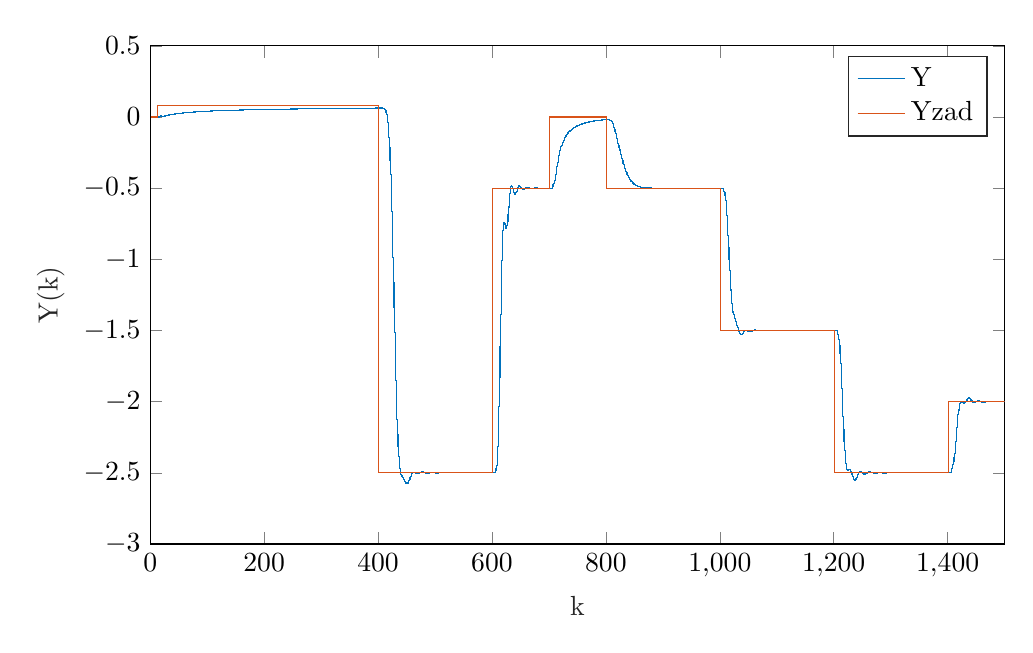
\begin{tikzpicture}

\begin{axis}[%
width=4.272in,
height=2.491in,
at={(0.717in,0.423in)},
scale only axis,
xmin=0,
xmax=1500,
xlabel style={font=\color{white!15!black}},
xlabel={k},
ymin=-3,
ymax=0.5,
ylabel style={font=\color{white!15!black}},
ylabel={Y(k)},
axis background/.style={fill=white},
legend style={legend cell align=left, align=left, draw=white!15!black}
]
\addplot[const plot, color=mycolor1] table[row sep=crcr] {%
1	0\\
2	0\\
3	0\\
4	0\\
5	0\\
6	0\\
7	0\\
8	0\\
9	0\\
10	0\\
11	0\\
12	0\\
13	0\\
14	0\\
15	0\\
16	0\\
17	0.00334251881758044\\
18	0.00682132589956547\\
19	0.00704162171120523\\
20	0.00627447743426751\\
21	0.00560428970171834\\
22	0.00522477015261361\\
23	0.00510683570109305\\
24	0.00545276086030931\\
25	0.00628451702151066\\
26	0.00737628866374661\\
27	0.00853060636273324\\
28	0.00964571911575367\\
29	0.0106765490515731\\
30	0.0116057732564279\\
31	0.0124463208117719\\
32	0.0132294339362455\\
33	0.0139835678152598\\
34	0.0147255384755444\\
35	0.015461931760978\\
36	0.0161926088145255\\
37	0.0169135330727078\\
38	0.017619621547013\\
39	0.0183070174177922\\
40	0.0189739381276443\\
41	0.0196203946947345\\
42	0.0202475100066409\\
43	0.0208568634006764\\
44	0.0214499966692187\\
45	0.022028138264434\\
46	0.0225921423351186\\
47	0.0231425666490333\\
48	0.0236797962639871\\
49	0.0242041521819811\\
50	0.0247159611998927\\
51	0.0252155853468876\\
52	0.0257034209715788\\
53	0.026179882196744\\
54	0.026645381666049\\
55	0.0271003161025166\\
56	0.0275450589536985\\
57	0.0279799591375161\\
58	0.0284053435568737\\
59	0.0288215210153823\\
60	0.0292287858581358\\
61	0.029627420551001\\
62	0.0300176971178683\\
63	0.0303998777359226\\
64	0.0307742148881238\\
65	0.0311409514013001\\
66	0.0315003205623341\\
67	0.0318525463767225\\
68	0.0321978439495371\\
69	0.0325364199334205\\
70	0.0328684729883722\\
71	0.0331941942157416\\
72	0.0335137675497014\\
73	0.0338273701054325\\
74	0.0341351724917505\\
75	0.03443733909801\\
76	0.0347340283633873\\
77	0.0350253930335413\\
78	0.035311580406848\\
79	0.0355927325705969\\
80	0.0358689866267732\\
81	0.036140474907021\\
82	0.0364073251766968\\
83	0.0366696608283012\\
84	0.0369276010648428\\
85	0.0371812610738118\\
86	0.0374307521924435\\
87	0.0376761820648824\\
88	0.0379176547917745\\
89	0.038155271072733\\
90	0.038389128342067\\
91	0.0386193208981258\\
92	0.0388459400265894\\
93	0.0390690741180197\\
94	0.039288808779975\\
95	0.0395052269439776\\
96	0.0397184089676059\\
97	0.0399284327319721\\
98	0.040135373734826\\
99	0.0403393051795129\\
100	0.0405402980599991\\
101	0.0407384212421652\\
102	0.0409337415415564\\
103	0.0411263237977671\\
104	0.0413162309456283\\
105	0.0415035240833564\\
106	0.0416882625378126\\
107	0.0418705039270143\\
108	0.0420503042200329\\
109	0.0422277177944032\\
110	0.0424027974911644\\
111	0.0425755946676456\\
112	0.0427461592481013\\
113	0.0429145397723003\\
114	0.0430807834421612\\
115	0.0432449361665266\\
116	0.0434070426041613\\
117	0.0435671462050562\\
118	0.0437252892501148\\
119	0.0438815128892953\\
120	0.0440358571782781\\
121	0.0441883611137245\\
122	0.0443390626671891\\
123	0.0444879988177452\\
124	0.0446352055833797\\
125	0.0447807180512117\\
126	0.0449245704065848\\
127	0.045066795961082\\
128	0.0452074271795101\\
129	0.0453464957058962\\
130	0.045484032388539\\
131	0.045620067304154\\
132	0.0457546297811517\\
133	0.0458877484220828\\
134	0.0460194511252873\\
135	0.0461497651057778\\
136	0.0462787169153904\\
137	0.0464063324622316\\
138	0.0465326370294499\\
139	0.04665765529336\\
140	0.046781411340944\\
141	0.0469039286867561\\
142	0.0470252302892531\\
143	0.0471453385665733\\
144	0.0472642754117866\\
145	0.0473820622076347\\
146	0.0474987198407822\\
147	0.0476142687155969\\
148	0.047728728767478\\
149	0.0478421194757481\\
150	0.0479544598761274\\
151	0.0480657685728032\\
152	0.0481760637501131\\
153	0.0482853631838532\\
154	0.0483936842522274\\
155	0.0485010439464497\\
156	0.0486074588810132\\
157	0.0487129453036368\\
158	0.0488175191049027\\
159	0.0489211958275947\\
160	0.0490239906757488\\
161	0.0491259185234255\\
162	0.0492269939232152\\
163	0.0493272311144841\\
164	0.0494266440313721\\
165	0.0495252463105492\\
166	0.0496230512987398\\
167	0.0497200720600238\\
168	0.0498163213829204\\
169	0.0499118117872634\\
170	0.0500065555308746\\
171	0.0501005646160425\\
172	0.0501938507958125\\
173	0.0502864255800954\\
174	0.0503783002415993\\
175	0.0504694858215928\\
176	0.0505599931355026\\
177	0.0506498327783529\\
178	0.0507390151300509\\
179	0.0508275503605239\\
180	0.0509154484347123\\
181	0.0510027191174234\\
182	0.0510893719780513\\
183	0.0511754163951654\\
184	0.0512608615609736\\
185	0.0513457164856633\\
186	0.0514299900016236\\
187	0.051513690767554\\
188	0.0515968272724607\\
189	0.0516794078395474\\
190	0.05176144063\\
191	0.0518429336466722\\
192	0.0519238947376721\\
193	0.0520043315998547\\
194	0.0520842517822223\\
195	0.0521636626892361\\
196	0.0522425715840413\\
197	0.0523209855916083\\
198	0.0523989117017931\\
199	0.0524763567723184\\
200	0.0525533275316789\\
201	0.0526298305819719\\
202	0.0527058724016561\\
203	0.0527814593482407\\
204	0.0528565976609065\\
205	0.052931293463061\\
206	0.0530055527648304\\
207	0.0530793814654884\\
208	0.0531527853558254\\
209	0.0532257701204595\\
210	0.0532983413400894\\
211	0.0533705044936936\\
212	0.0534422649606745\\
213	0.0535136280229514\\
214	0.0535845988670022\\
215	0.0536551825858558\\
216	0.053725384181037\\
217	0.0537952085644648\\
218	0.0538646605603044\\
219	0.0539337449067768\\
220	0.0540024662579243\\
221	0.0540708291853348\\
222	0.0541388381798255\\
223	0.0542064976530873\\
224	0.0542738119392905\\
225	0.0543407852966539\\
226	0.0544074219089761\\
227	0.0544737258871336\\
228	0.0545397012705423\\
229	0.0546053520285868\\
230	0.0546706820620167\\
231	0.0547356952043115\\
232	0.0548003952230135\\
233	0.0548647858210319\\
234	0.0549288706379165\\
235	0.0549926532511038\\
236	0.055056137177134\\
237	0.0551193258728422\\
238	0.0551822227365218\\
239	0.0552448311090637\\
240	0.0553071542750689\\
241	0.0553691954639374\\
242	0.0554309578509332\\
243	0.0554924445582257\\
244	0.0555536586559091\\
245	0.0556146031629987\\
246	0.0556752810484064\\
247	0.0557356952318952\\
248	0.0557958485850124\\
249	0.0558557439320038\\
250	0.0559153840507076\\
251	0.0559747716734298\\
252	0.0560339094878005\\
253	0.0560928001376127\\
254	0.0561514462236427\\
255	0.0562098503044538\\
256	0.0562680148971832\\
257	0.0563259424783116\\
258	0.0563836354844181\\
259	0.0564410963129178\\
260	0.0564983273227857\\
261	0.0565553308352649\\
262	0.0566121091345596\\
263	0.056668664468515\\
264	0.0567249990492829\\
265	0.0567811150539732\\
266	0.0568370146252924\\
267	0.0568926998721698\\
268	0.05694817287037\\
269	0.0570034356630935\\
270	0.0570584902615651\\
271	0.057113338645611\\
272	0.0571679827642232\\
273	0.0572224245361141\\
274	0.0572766658502583\\
275	0.0573307085664253\\
276	0.0573845545157008\\
277	0.0574382055009976\\
278	0.0574916632975566\\
279	0.0575449296534382\\
280	0.0575980062900038\\
281	0.0576508949023875\\
282	0.0577035971599596\\
283	0.05775611470678\\
284	0.0578084491620435\\
285	0.057860602120516\\
286	0.0579125751529627\\
287	0.0579643698065676\\
288	0.0580159876053454\\
289	0.0580674300505451\\
290	0.0581186986210459\\
291	0.0581697947737459\\
292	0.0582207199439429\\
293	0.0582714755457083\\
294	0.0583220629722539\\
295	0.0583724835962915\\
296	0.0584227387703856\\
297	0.0584728298273004\\
298	0.058522758080339\\
299	0.0585725248236768\\
300	0.0586221313326891\\
301	0.0586715788642718\\
302	0.0587208686571564\\
303	0.0587700019322196\\
304	0.0588189798927863\\
305	0.0588678037249277\\
306	0.0589164745977534\\
307	0.0589649936636988\\
308	0.0590133620588062\\
309	0.0590615809030014\\
310	0.0591096513003654\\
311	0.0591575743394004\\
312	0.0592053510932916\\
313	0.0592529826201641\\
314	0.0593004699633345\\
315	0.0593478141515592\\
316	0.0593950161992765\\
317	0.0594420771068462\\
318	0.0594889978607831\\
319	0.0595357794339878\\
320	0.0595824227859721\\
321	0.0596289288630811\\
322	0.0596752985987114\\
323	0.0597215329135245\\
324	0.0597676327156577\\
325	0.0598135989009297\\
326	0.0598594323530444\\
327	0.0599051339437891\\
328	0.0599507045332307\\
329	0.0599961449699074\\
330	0.0600414560910182\\
331	0.0600866387226073\\
332	0.0601316936797471\\
333	0.0601766217667168\\
334	0.060221423777178\\
335	0.060266100494348\\
336	0.0603106526911687\\
337	0.060355081130474\\
338	0.0603993865651532\\
339	0.060443569738312\\
340	0.0604876313834309\\
341	0.0605315722245203\\
342	0.0605753929762732\\
343	0.0606190943442153\\
344	0.0606626770248527\\
345	0.0607061417058164\\
346	0.060749489066005\\
347	0.0607927197757243\\
348	0.0608358344968252\\
349	0.0608788338828387\\
350	0.0609217185791086\\
351	0.0609644892229224\\
352	0.0610071464436394\\
353	0.0610496908628169\\
354	0.0610921230943341\\
355	0.061134443744514\\
356	0.0611766534122435\\
357	0.0612187526890906\\
358	0.0612607421594205\\
359	0.0613026224005095\\
360	0.0613443939826566\\
361	0.0613860574692935\\
362	0.0614276134170929\\
363	0.0614690623760746\\
364	0.06151040488971\\
365	0.0615516414950251\\
366	0.0615927727227011\\
367	0.0616337990971739\\
368	0.0616747211367319\\
369	0.0617155393536116\\
370	0.0617562542540925\\
371	0.0617968663385895\\
372	0.0618373761017443\\
373	0.0618777840325153\\
374	0.0619180906142655\\
375	0.0619582963248497\\
376	0.0619984016366994\\
377	0.0620384070169071\\
378	0.0620783129273085\\
379	0.062118119824564\\
380	0.0621578281602379\\
381	0.0621974383808778\\
382	0.0622369509280909\\
383	0.0622763662386205\\
384	0.0623156847444202\\
385	0.0623549068727277\\
386	0.0623940330461371\\
387	0.0624330636826693\\
388	0.0624719991958427\\
389	0.0625108399947412\\
390	0.0625495864840823\\
391	0.0625882390642831\\
392	0.0626267981315262\\
393	0.0626652640778238\\
394	0.0627036372910807\\
395	0.0627419181551569\\
396	0.0627801070499287\\
397	0.0628182043513491\\
398	0.0628562104315065\\
399	0.0628941256586836\\
400	0.0629319503974143\\
401	0.0629696850085404\\
402	0.0630073298492669\\
403	0.0630448852732165\\
404	0.0630823516304834\\
405	0.0631197292676862\\
406	0.063108597482763\\
407	0.0618525804223609\\
408	0.062087764817241\\
409	0.061195680021135\\
410	0.0590226607675442\\
411	0.0556291046046728\\
412	0.0507297757048514\\
413	0.0435566155381813\\
414	0.0328390060725044\\
415	0.0168569196204437\\
416	-0.00642888115499\\
417	-0.0391845641636356\\
418	-0.0834919386180635\\
419	-0.141169561102237\\
420	-0.213662152032099\\
421	-0.302007458379358\\
422	-0.406866522191738\\
423	-0.52859150667748\\
424	-0.666994466374835\\
425	-0.820545974324493\\
426	-0.986391987354576\\
427	-1.1607392357771\\
428	-1.33911943394609\\
429	-1.51662452129564\\
430	-1.68827509293188\\
431	-1.84897966194082\\
432	-1.99459072966043\\
433	-2.12224753054546\\
434	-2.23022773655396\\
435	-2.31797932718926\\
436	-2.38622875960895\\
437	-2.43682834986987\\
438	-2.47242433144607\\
439	-2.49613346562344\\
440	-2.51122610444077\\
441	-2.52078908330997\\
442	-2.52743523400552\\
443	-2.53312111583988\\
444	-2.53907149086547\\
445	-2.54579359158328\\
446	-2.55317371225445\\
447	-2.56063892732906\\
448	-2.56735260423367\\
449	-2.57241354869814\\
450	-2.57503598304338\\
451	-2.57469125204808\\
452	-2.57119614666411\\
453	-2.56474076007703\\
454	-2.5558578982308\\
455	-2.5453435172054\\
456	-2.53414352968361\\
457	-2.52322626076816\\
458	-2.51346049679643\\
459	-2.50551620030229\\
460	-2.49979970096899\\
461	-2.49642887620142\\
462	-2.49524759106341\\
463	-2.4958733973252\\
464	-2.49776883279745\\
465	-2.50032479891274\\
466	-2.50294428146658\\
467	-2.50511586042215\\
468	-2.50646873817904\\
469	-2.50680406494442\\
470	-2.50610077804603\\
471	-2.50449759550521\\
472	-2.50225579478569\\
473	-2.49970957691269\\
474	-2.49721188521968\\
475	-2.49508342018609\\
476	-2.49357137816624\\
477	-2.49282242979257\\
478	-2.49287203413337\\
479	-2.49364976158356\\
480	-2.49499821319398\\
481	-2.49670161030288\\
482	-2.4985193014657\\
483	-2.5002193044188\\
484	-2.50160749822488\\
485	-2.50254907602437\\
486	-2.50298019499545\\
487	-2.50290922861698\\
488	-2.50240844375182\\
489	-2.50159811313222\\
490	-2.50062589160602\\
491	-2.49964464873018\\
492	-2.49879184767037\\
493	-2.49817304717784\\
494	-2.49785129182004\\
495	-2.49784319013845\\
496	-2.49812151095567\\
497	-2.49862328627646\\
498	-2.49926179198672\\
499	-2.49994043923992\\
500	-2.50056656181233\\
501	-2.50106330211674\\
502	-2.50137822596535\\
503	-2.50148785876333\\
504	-2.50139794920367\\
505	-2.50113984711133\\
506	-2.50076385703418\\
507	-2.50033074514568\\
508	-2.49990270617195\\
509	-2.49953503935064\\
510	-2.49926956361681\\
511	-2.49913046789787\\
512	-2.49912289950567\\
513	-2.49923420097874\\
514	-2.49943736560638\\
515	-2.49969603356758\\
516	-2.49997021690343\\
517	-2.50022192775463\\
518	-2.50041997979802\\
519	-2.5005434141478\\
520	-2.50058323611032\\
521	-2.50054240227999\\
522	-2.50043423375277\\
523	-2.50027962130011\\
524	-2.50010351152585\\
525	-2.49993120942478\\
526	-2.49978500366454\\
527	-2.49968152762979\\
528	-2.49963013063101\\
529	-2.49963237271586\\
530	-2.49968259687033\\
531	-2.49976939504695\\
532	-2.49987768522557\\
533	-2.49999106472986\\
534	-2.50009410227717\\
535	-2.50017427309731\\
536	-2.50022331795368\\
537	-2.50023790457109\\
538	-2.50021957392046\\
539	-2.50017404976435\\
540	-2.50011006598728\\
541	-2.50003791442987\\
542	-2.49996793259962\\
543	-2.4999091366578\\
544	-2.49986816537667\\
545	-2.49984864315094\\
546	-2.49985100405202\\
547	-2.49987275392461\\
548	-2.49990909210644\\
549	-2.4999537748412\\
550	-2.50000008244312\\
551	-2.50004175242498\\
552	-2.50007375907059\\
553	-2.50009285210293\\
554	-2.5000978075534\\
555	-2.50008938653198\\
556	-2.50007003651479\\
557	-2.50004340024384\\
558	-2.50001371619362\\
559	-2.49998520046753\\
560	-2.49996149345329\\
561	-2.49994523769509\\
562	-2.49993782949121\\
563	-2.4999393595713\\
564	-2.49994873174897\\
565	-2.49996392610462\\
566	-2.49998235755799\\
567	-2.50000127304171\\
568	-2.50001813108433\\
569	-2.50003091554934\\
570	-2.50003834877582\\
571	-2.50003998609416\\
572	-2.50003619112181\\
573	-2.50002800701315\\
574	-2.50001695103266\\
575	-2.5000047671905\\
576	-2.4999931737344\\
577	-2.49998363929052\\
578	-2.49997721429026\\
579	-2.49997443436865\\
580	-2.49997530126525\\
581	-2.49997933599125\\
582	-2.49998569002735\\
583	-2.49999329409457\\
584	-2.50000102113614\\
585	-2.50000784061299\\
586	-2.50001294465006\\
587	-2.500015832226\\
588	-2.50001634450779\\
589	-2.5000146515595\\
590	-2.50001119703865\\
591	-2.50000661236941\\
592	-2.50000161475525\\
593	-2.4999969040873\\
594	-2.49999307244461\\
595	-2.49999053685324\\
596	-2.49998950183888\\
597	-2.49998995372793\\
598	-2.49999168427238\\
599	-2.4999943375523\\
600	-2.49999747164707\\
601	-2.50000062547156\\
602	-2.50000338145326\\
603	-2.50000541620724\\
604	-2.50000653373134\\
605	-2.5000066784955\\
606	-2.48494174931172\\
607	-2.47119211030231\\
608	-2.44884809676126\\
609	-2.40122828628753\\
610	-2.31787862130965\\
611	-2.19562755295039\\
612	-2.03299621564262\\
613	-1.83337729079254\\
614	-1.61117384022293\\
615	-1.38722990381947\\
616	-1.1815280400016\\
617	-1.00963858784038\\
618	-0.880878384033185\\
619	-0.797230117288416\\
620	-0.754177735799304\\
621	-0.742694433914748\\
622	-0.75123897380697\\
623	-0.767520424358011\\
624	-0.780262991792702\\
625	-0.780863718806716\\
626	-0.764628155867296\\
627	-0.731333040762184\\
628	-0.684895436146171\\
629	-0.632054191879385\\
630	-0.580419599194855\\
631	-0.536612962741626\\
632	-0.505057815640161\\
633	-0.487535392419528\\
634	-0.4833318107524\\
635	-0.48976599069336\\
636	-0.50293037858477\\
637	-0.518503021077315\\
638	-0.532509784311615\\
639	-0.541940962700535\\
640	-0.545146115923748\\
641	-0.54195105399516\\
642	-0.533483779001086\\
643	-0.521763017417104\\
644	-0.509163862863529\\
645	-0.497896847510464\\
646	-0.489611090457249\\
647	-0.485178290468889\\
648	-0.484660609039322\\
649	-0.487429315450165\\
650	-0.492383936118497\\
651	-0.498217533747161\\
652	-0.503677306262837\\
653	-0.50777822407978\\
654	-0.509939720544641\\
655	-0.510030866191536\\
656	-0.508326825630132\\
657	-0.505395961959841\\
658	-0.501948729849325\\
659	-0.498683289395364\\
660	-0.496158127867867\\
661	-0.494711372830498\\
662	-0.494433797346577\\
663	-0.49519117421842\\
664	-0.49668358839705\\
665	-0.49852511100093\\
666	-0.500326564732482\\
667	-0.501766302171738\\
668	-0.50263819154911\\
669	-0.502871497848986\\
670	-0.502523102301105\\
671	-0.501747513862526\\
672	-0.500753509902533\\
673	-0.499757479566644\\
674	-0.498942634638437\\
675	-0.498430699443809\\
676	-0.498269290915004\\
677	-0.49843478192035\\
678	-0.498847658986649\\
679	-0.499395623016228\\
680	-0.499959056039296\\
681	-0.500433894904947\\
682	-0.500748174708877\\
683	-0.500870204289285\\
684	-0.500808153746848\\
685	-0.50060243157607\\
686	-0.500313344482127\\
687	-0.500007023813288\\
688	-0.499742464687793\\
689	-0.499561877538131\\
690	-0.499485599059328\\
691	-0.499511778981299\\
692	-0.499620154489169\\
693	-0.499778589719895\\
694	-0.499950763372297\\
695	-0.500103430656022\\
696	-0.500212005618701\\
697	-0.500263706843962\\
698	-0.500258068010279\\
699	-0.500205124991922\\
700	-0.500121967441924\\
701	-0.500028536098514\\
702	-0.499943549289582\\
703	-0.499881281973132\\
704	-0.499849652789448\\
705	-0.499849765162954\\
706	-0.48581982239339\\
707	-0.474990269538938\\
708	-0.467642976893124\\
709	-0.458095874748353\\
710	-0.443342806777156\\
711	-0.425524620998392\\
712	-0.404293436320976\\
713	-0.378972059423545\\
714	-0.350963785319601\\
715	-0.32271410848308\\
716	-0.295900793601818\\
717	-0.271670948668872\\
718	-0.250903220404157\\
719	-0.233867705063716\\
720	-0.220111476328016\\
721	-0.208806054835933\\
722	-0.199061024647939\\
723	-0.190067874762619\\
724	-0.181223391982717\\
725	-0.172231452708753\\
726	-0.163094792716769\\
727	-0.154016708035256\\
728	-0.145285975219329\\
729	-0.137177663638038\\
730	-0.129878812474669\\
731	-0.1234522268445\\
732	-0.117842544766527\\
733	-0.112911370625142\\
734	-0.108483313431964\\
735	-0.104389359869079\\
736	-0.100498498024955\\
737	-0.0967325773736974\\
738	-0.0930647315989403\\
739	-0.0895062034136207\\
740	-0.0860880917977225\\
741	-0.0828438861423317\\
742	-0.0797968344405446\\
743	-0.076953898603789\\
744	-0.0743058745413442\\
745	-0.0718317924079887\\
746	-0.0695051912170109\\
747	-0.0673001120020288\\
748	-0.0651953630315971\\
749	-0.0631764769739474\\
750	-0.0612355445319407\\
751	-0.0593695992848881\\
752	-0.0575783948473746\\
753	-0.0558623136121269\\
754	-0.0542208852852018\\
755	-0.0526520892852085\\
756	-0.0511523602707494\\
757	-0.0497170620832841\\
758	-0.0483411508540586\\
759	-0.0470197897910036\\
760	-0.0457487679063839\\
761	-0.0445246740442678\\
762	-0.0433448571884769\\
763	-0.0422072496364973\\
764	-0.0411101403188464\\
765	-0.0400519699368565\\
766	-0.0390311904179164\\
767	-0.0380462005787626\\
768	-0.0370953463583432\\
769	-0.0361769613561583\\
770	-0.0352894213584155\\
771	-0.0344311920382783\\
772	-0.0336008580795649\\
773	-0.0327971310054606\\
774	-0.0320188396292113\\
775	-0.0312649103553908\\
776	-0.0305343448179202\\
777	-0.0298262005308801\\
778	-0.0291395775449147\\
779	-0.0284736115588173\\
780	-0.0278274721570655\\
781	-0.0272003640336248\\
782	-0.0265915290956468\\
783	-0.0260002479125879\\
784	-0.025425839745623\\
785	-0.0248676610856931\\
786	-0.0243251030895937\\
787	-0.0237975884930455\\
788	-0.0232845685447443\\
789	-0.0227855203359851\\
790	-0.0222999446901973\\
791	-0.0218273645964846\\
792	-0.0213673240583535\\
793	-0.0209193871891206\\
794	-0.0204831374031716\\
795	-0.0200581766018979\\
796	-0.019644124310002\\
797	-0.0192406167642825\\
798	-0.0188473059845466\\
799	-0.0184638588646392\\
800	-0.0180899563156608\\
801	-0.0177252924801906\\
802	-0.017369574022073\\
803	-0.0170225194853197\\
804	-0.0166838587097241\\
805	-0.016353332289666\\
806	-0.0209257895708119\\
807	-0.024590293198601\\
808	-0.0255185314479029\\
809	-0.0274226119954852\\
810	-0.0317740390666369\\
811	-0.0384262799798205\\
812	-0.0472243673995788\\
813	-0.0583995789582614\\
814	-0.0716673846188672\\
815	-0.0863740248144801\\
816	-0.101982908539189\\
817	-0.11813962892031\\
818	-0.134544458984383\\
819	-0.150970725880677\\
820	-0.167321358158781\\
821	-0.183588279872564\\
822	-0.199785749413162\\
823	-0.215924538658888\\
824	-0.232002329769905\\
825	-0.247987365803362\\
826	-0.263810328795378\\
827	-0.279372782821903\\
828	-0.294561690213241\\
829	-0.309262472697387\\
830	-0.323371327970699\\
831	-0.336806197529811\\
832	-0.349513245172451\\
833	-0.361467883679102\\
834	-0.372671774587418\\
835	-0.383147176355589\\
836	-0.39292966669752\\
837	-0.402060625985825\\
838	-0.410580897758721\\
839	-0.418526441290754\\
840	-0.425926200305785\\
841	-0.432802062153944\\
842	-0.439170482142505\\
843	-0.44504509652022\\
844	-0.450439581078036\\
845	-0.455370122856428\\
846	-0.459857062455538\\
847	-0.463925485909997\\
848	-0.467604777049863\\
849	-0.47092733982892\\
850	-0.473926824409662\\
851	-0.476636231759539\\
852	-0.479086239878886\\
853	-0.481304006654117\\
854	-0.483312582351334\\
855	-0.485130937037208\\
856	-0.486774499698337\\
857	-0.488256032662102\\
858	-0.489586634316222\\
859	-0.490776674187873\\
860	-0.491836508903514\\
861	-0.492776892117727\\
862	-0.493609061369439\\
863	-0.494344546650251\\
864	-0.494994789366901\\
865	-0.495570681159409\\
866	-0.49608212952307\\
867	-0.496537735487753\\
868	-0.496944634682631\\
869	-0.497308515042203\\
870	-0.497633789776682\\
871	-0.497923878820066\\
872	-0.498181538984628\\
873	-0.498409182935099\\
874	-0.498609137887968\\
875	-0.498783813001326\\
876	-0.498935765347768\\
877	-0.499067673911711\\
878	-0.499182245881658\\
879	-0.49928208764852\\
880	-0.499369573924604\\
881	-0.499446743184711\\
882	-0.499515238111571\\
883	-0.499576298302347\\
884	-0.499630801536807\\
885	-0.499679341343153\\
886	-0.49972232361362\\
887	-0.499760063971734\\
888	-0.499792870058835\\
889	-0.499821097895564\\
890	-0.499845177685336\\
891	-0.499865610539921\\
892	-0.499882942522373\\
893	-0.49989772540823\\
894	-0.499910474408012\\
895	-0.499921631952263\\
896	-0.499931544028139\\
897	-0.499940452175871\\
898	-0.499948500838188\\
899	-0.49995575693261\\
900	-0.499962236707494\\
901	-0.499967934320009\\
902	-0.499972847067239\\
903	-0.499976993547721\\
904	-0.499980422852168\\
905	-0.499983214773291\\
906	-0.499985472629651\\
907	-0.499987311368681\\
908	-0.499988844036652\\
909	-0.499990169501101\\
910	-0.499991363617065\\
911	-0.49999247504466\\
912	-0.499993525875728\\
913	-0.499994516312786\\
914	-0.49999543200976\\
915	-0.499996252402987\\
916	-0.499996958429155\\
917	-0.499997538377804\\
918	-0.499997991151935\\
919	-0.499998326788201\\
920	-0.499998564604703\\
921	-0.499998729714784\\
922	-0.499998848824485\\
923	-0.499998946216261\\
924	-0.499999040644805\\
925	-0.499999143589609\\
926	-0.499999258990415\\
927	-0.499999384299799\\
928	-0.499999512470796\\
929	-0.499999634384395\\
930	-0.499999741216586\\
931	-0.499999826331627\\
932	-0.499999886437214\\
933	-0.499999921911558\\
934	-0.499999936376281\\
935	-0.499999935714283\\
936	-0.499999926801446\\
937	-0.499999916231074\\
938	-0.499999909267731\\
939	-0.499999909188343\\
940	-0.499999917073142\\
941	-0.499999932017051\\
942	-0.499999951659804\\
943	-0.499999972890461\\
944	-0.499999992572312\\
945	-0.500000008154044\\
946	-0.500000018074341\\
947	-0.50000002191891\\
948	-0.500000020340272\\
949	-0.500000014792169\\
950	-0.500000007156125\\
951	-0.499999999345292\\
952	-0.499999992961647\\
953	-0.499999989061075\\
954	-0.499999988052746\\
955	-0.499999989730609\\
956	-0.499999993411054\\
957	-0.49999999813543\\
958	-0.500000002890653\\
959	-0.500000006805023\\
960	-0.500000009287517\\
961	-0.50000001009399\\
962	-0.500000009319591\\
963	-0.500000007330226\\
964	-0.500000004655034\\
965	-0.50000000186552\\
966	-0.499999999465473\\
967	-0.499999997810088\\
968	-0.499999997064536\\
969	-0.499999997203474\\
970	-0.499999998045256\\
971	-0.499999999309294\\
972	-0.500000000682524\\
973	-0.500000001881499\\
974	-0.50000000269946\\
975	-0.500000003032147\\
976	-0.500000002880926\\
977	-0.500000002336185\\
978	-0.500000001547063\\
979	-0.500000000685143\\
980	-0.499999999909668\\
981	-0.499999999340369\\
982	-0.499999999041697\\
983	-0.499999999019554\\
984	-0.499999999229211\\
985	-0.499999999591217\\
986	-0.500000000011188\\
987	-0.500000000399263\\
988	-0.500000000685728\\
989	-0.500000000830567\\
990	-0.500000000826122\\
991	-0.500000000693456\\
992	-0.500000000474047\\
993	-0.500000000219043\\
994	-0.499999999978425\\
995	-0.499999999792054\\
996	-0.499999999683947\\
997	-0.49999999966033\\
998	-0.499999999711231\\
999	-0.499999999814784\\
1000	-0.499999999943031\\
1001	-0.500000000067945\\
1002	-0.500000000166537\\
1003	-0.500000000224251\\
1004	-0.500000000236306\\
1005	-0.500000000207047\\
1006	-0.512415440234685\\
1007	-0.522500171139069\\
1008	-0.533557841350533\\
1009	-0.553731163950725\\
1010	-0.586950398158947\\
1011	-0.632196878019564\\
1012	-0.689351399708103\\
1013	-0.757920865476842\\
1014	-0.835131876257141\\
1015	-0.9168603854388\\
1016	-0.999161597310075\\
1017	-1.07843626813624\\
1018	-1.15136727605897\\
1019	-1.21539522242919\\
1020	-1.26912383570589\\
1021	-1.3122813068812\\
1022	-1.34553742583861\\
1023	-1.37034736959125\\
1024	-1.3887019468538\\
1025	-1.40277242351492\\
1026	-1.41458236799391\\
1027	-1.42577378302689\\
1028	-1.43745627053171\\
1029	-1.45014151682204\\
1030	-1.46377578126906\\
1031	-1.47785390984425\\
1032	-1.49157992464568\\
1033	-1.50404565326214\\
1034	-1.51440482930711\\
1035	-1.52201933930417\\
1036	-1.52655813796424\\
1037	-1.52803917357811\\
1038	-1.52681400343409\\
1039	-1.52350218047904\\
1040	-1.51888947380448\\
1041	-1.51380916915715\\
1042	-1.50902679191457\\
1043	-1.50514569389547\\
1044	-1.50254557975786\\
1045	-1.50135951680338\\
1046	-1.5014884019067\\
1047	-1.50264640636928\\
1048	-1.5044273104988\\
1049	-1.50637998452987\\
1050	-1.50808137730602\\
1051	-1.50919697873363\\
1052	-1.50952148858613\\
1053	-1.50899591636698\\
1054	-1.50770106445662\\
1055	-1.5058308000766\\
1056	-1.50365120775414\\
1057	-1.50145324497498\\
1058	-1.49950672209694\\
1059	-1.49802237511333\\
1060	-1.49712680452338\\
1061	-1.49685255889792\\
1062	-1.49714311524805\\
1063	-1.49787034516268\\
1064	-1.49886052265312\\
1065	-1.49992415307842\\
1066	-1.50088488522596\\
1067	-1.50160341739882\\
1068	-1.50199346139498\\
1069	-1.5020282794313\\
1070	-1.50173783132571\\
1071	-1.50119794046398\\
1072	-1.50051391905916\\
1073	-1.49980165990533\\
1074	-1.4991692589066\\
1075	-1.49870182160815\\
1076	-1.49845134139621\\
1077	-1.49843257524616\\
1078	-1.49862485465521\\
1079	-1.4989789058507\\
1080	-1.49942712597742\\
1081	-1.49989543238406\\
1082	-1.50031478166608\\
1083	-1.50063071099483\\
1084	-1.50080971981205\\
1085	-1.50084189700058\\
1086	-1.50073981078478\\
1087	-1.50053422477384\\
1088	-1.50026761026632\\
1089	-1.49998664588372\\
1090	-1.49973491673957\\
1091	-1.4995468644263\\
1092	-1.49944373988544\\
1093	-1.49943193380086\\
1094	-1.49950366854442\\
1095	-1.49963969117231\\
1096	-1.49981335379414\\
1097	-1.4999953322741\\
1098	-1.50015822297292\\
1099	-1.5002803579011\\
1100	-1.50034836443644\\
1101	-1.50035823061801\\
1102	-1.50031488165297\\
1103	-1.50023049095399\\
1104	-1.50012191068699\\
1105	-1.50000769455203\\
1106	-1.49990519422493\\
1107	-1.49982814773381\\
1108	-1.49978506016664\\
1109	-1.49977852792479\\
1110	-1.49980550271961\\
1111	-1.49985835411002\\
1112	-1.49992648779483\\
1113	-1.49999822198969\\
1114	-1.50006261888502\\
1115	-1.50011100773479\\
1116	-1.50013800990391\\
1117	-1.50014196973636\\
1118	-1.50012479260497\\
1119	-1.50009127827643\\
1120	-1.50004810219954\\
1121	-1.50000263242816\\
1122	-1.49996177362295\\
1123	-1.49993100478097\\
1124	-1.49991373076637\\
1125	-1.4999110085875\\
1126	-1.49992164775006\\
1127	-1.49994262923296\\
1128	-1.49996974696785\\
1129	-1.49999835356343\\
1130	-1.50002408961519\\
1131	-1.50004349147489\\
1132	-1.5000544015967\\
1133	-1.50005614276067\\
1134	-1.50004945629431\\
1135	-1.50003623900478\\
1136	-1.50001913928376\\
1137	-1.50000108693213\\
1138	-1.49998483286982\\
1139	-1.49997256516145\\
1140	-1.49996564936551\\
1141	-1.49996451775387\\
1142	-1.49996870744355\\
1143	-1.4999770256416\\
1144	-1.49998780394021\\
1145	-1.49999919468673\\
1146	-1.50000946139738\\
1147	-1.50001722128215\\
1148	-1.50002160952975\\
1149	-1.50002234977301\\
1150	-1.50001973060475\\
1151	-1.50001450180488\\
1152	-1.50000771422757\\
1153	-1.50000053295602\\
1154	-1.49999405403251\\
1155	-1.49998915125029\\
1156	-1.49998637220391\\
1157	-1.49998589348136\\
1158	-1.49998753513395\\
1159	-1.49999082585207\\
1160	-1.49999510377336\\
1161	-1.49999963426502\\
1162	-1.50000372556352\\
1163	-1.50000682554865\\
1164	-1.50000858751416\\
1165	-1.50000889866315\\
1166	-1.5000078712045\\
1167	-1.50000580142365\\
1168	-1.50000310621313\\
1169	-1.50000024882178\\
1170	-1.49999766588353\\
1171	-1.49999570628705\\
1172	-1.4999945895621\\
1173	-1.4999943877616\\
1174	-1.49999503093988\\
1175	-1.49999633285688\\
1176	-1.49999803093863\\
1177	-1.49999983308374\\
1178	-1.50000146370776\\
1179	-1.50000270235666\\
1180	-1.50000341003588\\
1181	-1.50000354073039\\
1182	-1.50000313803764\\
1183	-1.50000231902622\\
1184	-1.50000124907709\\
1185	-1.50000011237719\\
1186	-1.49999908286527\\
1187	-1.49999829984114\\
1188	-1.49999785130752\\
1189	-1.49999776664608\\
1190	-1.49999801868611\\
1191	-1.49999853384068\\
1192	-1.49999920794641\\
1193	-1.49999992486364\\
1194	-1.50000057480934\\
1195	-1.50000106976364\\
1196	-1.50000135400907\\
1197	-1.50000140878677\\
1198	-1.50000125102663\\
1199	-1.50000092698245\\
1200	-1.5000005022595\\
1201	-1.50000005008935\\
1202	-1.49999963976187\\
1203	-1.49999932689373\\
1204	-1.49999914676044\\
1205	-1.4999991113365\\
1206	-1.51369953632264\\
1207	-1.52606030802534\\
1208	-1.54031212541816\\
1209	-1.56524972157796\\
1210	-1.60564211620385\\
1211	-1.6607458313089\\
1212	-1.73053419583599\\
1213	-1.81443497923858\\
1214	-1.90920550453315\\
1215	-2.00837330283341\\
1216	-2.10560322904113\\
1217	-2.19658520357174\\
1218	-2.27756681379569\\
1219	-2.34536258685289\\
1220	-2.39833674139913\\
1221	-2.4365996008314\\
1222	-2.46146145689584\\
1223	-2.47513030539658\\
1224	-2.48053727078683\\
1225	-2.4809190492509\\
1226	-2.47931098652289\\
1227	-2.47821114517815\\
1228	-2.47939265665328\\
1229	-2.48379255632123\\
1230	-2.49150830409769\\
1231	-2.50192243978358\\
1232	-2.51390695068585\\
1233	-2.52605624907455\\
1234	-2.53692544025767\\
1235	-2.54525176654025\\
1236	-2.55012965007039\\
1237	-2.55111866404858\\
1238	-2.54827835063552\\
1239	-2.54213209115668\\
1240	-2.53356899773369\\
1241	-2.52370177850351\\
1242	-2.51370501424602\\
1243	-2.50465890269042\\
1244	-2.49741985037345\\
1245	-2.49253323169993\\
1246	-2.49019592492516\\
1247	-2.49026815802487\\
1248	-2.49232747382449\\
1249	-2.49575310962311\\
1250	-2.49982674477991\\
1251	-2.50383517340448\\
1252	-2.50716177964967\\
1253	-2.50935637280992\\
1254	-2.51017654615993\\
1255	-2.50959784801872\\
1256	-2.50779426415114\\
1257	-2.50509429909486\\
1258	-2.50192079459958\\
1259	-2.49872414390289\\
1260	-2.49591858260412\\
1261	-2.49382985876673\\
1262	-2.49266014933699\\
1263	-2.49247309325737\\
1264	-2.49319877675814\\
1265	-2.49465587403259\\
1266	-2.49658621588168\\
1267	-2.49869597578413\\
1268	-2.50069744001786\\
1269	-2.50234587940309\\
1270	-2.50346721146372\\
1271	-2.50397373656076\\
1272	-2.50386702653287\\
1273	-2.50322880615331\\
1274	-2.50220217445219\\
1275	-2.50096658189238\\
1276	-2.49971049466027\\
1277	-2.49860560942244\\
1278	-2.49778589097105\\
1279	-2.49733372581853\\
1280	-2.49727429641683\\
1281	-2.49757807232818\\
1282	-2.49817025356588\\
1283	-2.49894521118991\\
1284	-2.49978352152107\\
1285	-2.50056910039867\\
1286	-2.50120418390451\\
1287	-2.50162040702946\\
1288	-2.50178491237144\\
1289	-2.50170117485293\\
1290	-2.50140495268956\\
1291	-2.50095637787746\\
1292	-2.5004296121251\\
1293	-2.49990167792082\\
1294	-2.49944202524816\\
1295	-2.49910414108473\\
1296	-2.4989201059071\\
1297	-2.49889851897882\\
1298	-2.49902572565058\\
1299	-2.49926985117577\\
1300	-2.49958682686311\\
1301	-2.49992741560101\\
1302	-2.50024421319188\\
1303	-2.50049770796943\\
1304	-2.50066069620791\\
1305	-2.5007206362665\\
1306	-2.50067983642717\\
1307	-2.50055366680558\\
1308	-2.50036722738629\\
1309	-2.50015106535192\\
1310	-2.49993660172735\\
1311	-2.49975190012263\\
1312	-2.49961830188075\\
1313	-2.49954828479807\\
1314	-2.49954470500947\\
1315	-2.49960138300808\\
1316	-2.49970482152321\\
1317	-2.49983671533955\\
1318	-2.49997684316978\\
1319	-2.50010592262998\\
1320	-2.50020805619646\\
1321	-2.50027248698988\\
1322	-2.50029450205065\\
1323	-2.50027544913327\\
1324	-2.50022195318429\\
1325	-2.50014451558192\\
1326	-2.50005574239764\\
1327	-2.49996847234752\\
1328	-2.4998940613244\\
1329	-2.49984103405342\\
1330	-2.49981424388886\\
1331	-2.49981460060468\\
1332	-2.49983934513593\\
1333	-2.49988278025846\\
1334	-2.49993731526534\\
1335	-2.4999946555831\\
1336	-2.50004696612619\\
1337	-2.50008785777995\\
1338	-2.5001130847463\\
1339	-2.50012088977445\\
1340	-2.50011198696356\\
1341	-2.50008922060465\\
1342	-2.50005697738542\\
1343	-2.50002045407595\\
1344	-2.49998489166936\\
1345	-2.49995488028476\\
1346	-2.49993381937801\\
1347	-2.49992358886881\\
1348	-2.4999244534203\\
1349	-2.4999351891495\\
1350	-2.4999533938088\\
1351	-2.49997592120645\\
1352	-2.49999937019703\\
1353	-2.50002055835705\\
1354	-2.50003691946907\\
1355	-2.50004678006185\\
1356	-2.50004949066013\\
1357	-2.50004540897314\\
1358	-2.50003575203757\\
1359	-2.50002234990008\\
1360	-2.50000734314508\\
1361	-2.49999286974614\\
1362	-2.49998078357993\\
1363	-2.49997243853363\\
1364	-2.4999685600968\\
1365	-2.49996921260811\\
1366	-2.49997385690361\\
1367	-2.49998148172573\\
1368	-2.49999078419814\\
1369	-2.50000037067736\\
1370	-2.50000894947731\\
1371	-2.50001549088456\\
1372	-2.5000193366503\\
1373	-2.50002024958307\\
1374	-2.50001840269663\\
1375	-2.50001431538692\\
1376	-2.50000875034534\\
1377	-2.50000258871978\\
1378	-2.49999670215018\\
1379	-2.49999183885519\\
1380	-2.49998853737627\\
1381	-2.49998707658013\\
1382	-2.49998746488149\\
1383	-2.49998946618332\\
1384	-2.49999265544369\\
1385	-2.49999649358345\\
1386	-2.50000040992947\\
1387	-2.50000388057591\\
1388	-2.50000649274576\\
1389	-2.50000798807152\\
1390	-2.50000828119993\\
1391	-2.5000074537367\\
1392	-2.50000572679522\\
1393	-2.50000341790656\\
1394	-2.50000088953291\\
1395	-2.49999849680934\\
1396	-2.49999654147743\\
1397	-2.49999523746232\\
1398	-2.49999469146482\\
1399	-2.49999489962445\\
1400	-2.49999575908564\\
1401	-2.4999970914526\\
1402	-2.49999867385277\\
1403	-2.50000027275462\\
1404	-2.50000167580781\\
1405	-2.50000271770786\\
1406	-2.48493911765285\\
1407	-2.4711909699576\\
1408	-2.45962805287144\\
1409	-2.44454648572264\\
1410	-2.42235399725001\\
1411	-2.39490819400443\\
1412	-2.36184708699484\\
1413	-2.32212008769797\\
1414	-2.27682188294519\\
1415	-2.22874065546497\\
1416	-2.18043361038513\\
1417	-2.13430974305953\\
1418	-2.09290816066121\\
1419	-2.05833655704649\\
1420	-2.0317305269576\\
1421	-2.01331114502977\\
1422	-2.0025590108815\\
1423	-1.9982840560221\\
1424	-1.99878361941026\\
1425	-2.00213704315332\\
1426	-2.0064855348203\\
1427	-2.01023440308794\\
1428	-2.01220911542269\\
1429	-2.01176052541133\\
1430	-2.00878472273838\\
1431	-2.00365813229044\\
1432	-1.99711603500472\\
1433	-1.99009771862619\\
1434	-1.98357822413253\\
1435	-1.97841278174851\\
1436	-1.97521791908997\\
1437	-1.9743018105891\\
1438	-1.97564643989932\\
1439	-1.97893783369594\\
1440	-1.98363491939015\\
1441	-1.98906296144841\\
1442	-1.99451597499021\\
1443	-1.99935354506345\\
1444	-2.00307977904271\\
1445	-2.00539541338788\\
1446	-2.00621838500336\\
1447	-2.00567287606798\\
1448	-2.00405117877543\\
1449	-2.00175616349345\\
1450	-1.99923425355273\\
1451	-1.9969092949787\\
1452	-1.9951265509346\\
1453	-1.99411360693698\\
1454	-1.99396180475027\\
1455	-1.99462851713001\\
1456	-1.99595764348317\\
1457	-1.99771351481694\\
1458	-1.99962213197715\\
1459	-2.0014133495779\\
1460	-2.0028581698975\\
1461	-2.0037965602118\\
1462	-2.00415293345961\\
1463	-2.00393838095993\\
1464	-2.00324064966383\\
1465	-2.00220446235341\\
1466	-2.00100588257285\\
1467	-1.99982490386306\\
1468	-1.99882027567057\\
1469	-1.99810985065667\\
1470	-1.99775861607288\\
1471	-1.99777526500349\\
1472	-1.99811688297642\\
1473	-1.99870024992332\\
1474	-1.99941751014335\\
1475	-2.0001536047743\\
1476	-2.00080289402266\\
1477	-2.00128277207483\\
1478	-2.00154271101712\\
1479	-2.0015679524547\\
1480	-2.00137787869075\\
1481	-2.00101982642696\\
1482	-2.00055966156597\\
1483	-2.00007075187048\\
1484	-1.999623031866\\
1485	-1.99927366829421\\
1486	-1.99906045566517\\
1487	-1.99899857410709\\
1488	-1.99908080897601\\
1489	-1.9992808422224\\
1490	-1.99955884248418\\
1491	-1.9998683451286\\
1492	-2.00016334095967\\
1493	-2.00040457529181\\
1494	-2.00056427000585\\
1495	-2.00062877842158\\
1496	-2.00059901735488\\
1497	-2.00048884322637\\
1498	-2.00032180638204\\
1499	-2.00012689824129\\
1500	-1.99993398288528\\
};
\addlegendentry{Y}

\addplot[const plot, color=mycolor2] table[row sep=crcr] {%
1	0\\
2	0\\
3	0\\
4	0\\
5	0\\
6	0\\
7	0\\
8	0\\
9	0\\
10	0\\
11	0\\
12	0.08\\
13	0.08\\
14	0.08\\
15	0.08\\
16	0.08\\
17	0.08\\
18	0.08\\
19	0.08\\
20	0.08\\
21	0.08\\
22	0.08\\
23	0.08\\
24	0.08\\
25	0.08\\
26	0.08\\
27	0.08\\
28	0.08\\
29	0.08\\
30	0.08\\
31	0.08\\
32	0.08\\
33	0.08\\
34	0.08\\
35	0.08\\
36	0.08\\
37	0.08\\
38	0.08\\
39	0.08\\
40	0.08\\
41	0.08\\
42	0.08\\
43	0.08\\
44	0.08\\
45	0.08\\
46	0.08\\
47	0.08\\
48	0.08\\
49	0.08\\
50	0.08\\
51	0.08\\
52	0.08\\
53	0.08\\
54	0.08\\
55	0.08\\
56	0.08\\
57	0.08\\
58	0.08\\
59	0.08\\
60	0.08\\
61	0.08\\
62	0.08\\
63	0.08\\
64	0.08\\
65	0.08\\
66	0.08\\
67	0.08\\
68	0.08\\
69	0.08\\
70	0.08\\
71	0.08\\
72	0.08\\
73	0.08\\
74	0.08\\
75	0.08\\
76	0.08\\
77	0.08\\
78	0.08\\
79	0.08\\
80	0.08\\
81	0.08\\
82	0.08\\
83	0.08\\
84	0.08\\
85	0.08\\
86	0.08\\
87	0.08\\
88	0.08\\
89	0.08\\
90	0.08\\
91	0.08\\
92	0.08\\
93	0.08\\
94	0.08\\
95	0.08\\
96	0.08\\
97	0.08\\
98	0.08\\
99	0.08\\
100	0.08\\
101	0.08\\
102	0.08\\
103	0.08\\
104	0.08\\
105	0.08\\
106	0.08\\
107	0.08\\
108	0.08\\
109	0.08\\
110	0.08\\
111	0.08\\
112	0.08\\
113	0.08\\
114	0.08\\
115	0.08\\
116	0.08\\
117	0.08\\
118	0.08\\
119	0.08\\
120	0.08\\
121	0.08\\
122	0.08\\
123	0.08\\
124	0.08\\
125	0.08\\
126	0.08\\
127	0.08\\
128	0.08\\
129	0.08\\
130	0.08\\
131	0.08\\
132	0.08\\
133	0.08\\
134	0.08\\
135	0.08\\
136	0.08\\
137	0.08\\
138	0.08\\
139	0.08\\
140	0.08\\
141	0.08\\
142	0.08\\
143	0.08\\
144	0.08\\
145	0.08\\
146	0.08\\
147	0.08\\
148	0.08\\
149	0.08\\
150	0.08\\
151	0.08\\
152	0.08\\
153	0.08\\
154	0.08\\
155	0.08\\
156	0.08\\
157	0.08\\
158	0.08\\
159	0.08\\
160	0.08\\
161	0.08\\
162	0.08\\
163	0.08\\
164	0.08\\
165	0.08\\
166	0.08\\
167	0.08\\
168	0.08\\
169	0.08\\
170	0.08\\
171	0.08\\
172	0.08\\
173	0.08\\
174	0.08\\
175	0.08\\
176	0.08\\
177	0.08\\
178	0.08\\
179	0.08\\
180	0.08\\
181	0.08\\
182	0.08\\
183	0.08\\
184	0.08\\
185	0.08\\
186	0.08\\
187	0.08\\
188	0.08\\
189	0.08\\
190	0.08\\
191	0.08\\
192	0.08\\
193	0.08\\
194	0.08\\
195	0.08\\
196	0.08\\
197	0.08\\
198	0.08\\
199	0.08\\
200	0.08\\
201	0.08\\
202	0.08\\
203	0.08\\
204	0.08\\
205	0.08\\
206	0.08\\
207	0.08\\
208	0.08\\
209	0.08\\
210	0.08\\
211	0.08\\
212	0.08\\
213	0.08\\
214	0.08\\
215	0.08\\
216	0.08\\
217	0.08\\
218	0.08\\
219	0.08\\
220	0.08\\
221	0.08\\
222	0.08\\
223	0.08\\
224	0.08\\
225	0.08\\
226	0.08\\
227	0.08\\
228	0.08\\
229	0.08\\
230	0.08\\
231	0.08\\
232	0.08\\
233	0.08\\
234	0.08\\
235	0.08\\
236	0.08\\
237	0.08\\
238	0.08\\
239	0.08\\
240	0.08\\
241	0.08\\
242	0.08\\
243	0.08\\
244	0.08\\
245	0.08\\
246	0.08\\
247	0.08\\
248	0.08\\
249	0.08\\
250	0.08\\
251	0.08\\
252	0.08\\
253	0.08\\
254	0.08\\
255	0.08\\
256	0.08\\
257	0.08\\
258	0.08\\
259	0.08\\
260	0.08\\
261	0.08\\
262	0.08\\
263	0.08\\
264	0.08\\
265	0.08\\
266	0.08\\
267	0.08\\
268	0.08\\
269	0.08\\
270	0.08\\
271	0.08\\
272	0.08\\
273	0.08\\
274	0.08\\
275	0.08\\
276	0.08\\
277	0.08\\
278	0.08\\
279	0.08\\
280	0.08\\
281	0.08\\
282	0.08\\
283	0.08\\
284	0.08\\
285	0.08\\
286	0.08\\
287	0.08\\
288	0.08\\
289	0.08\\
290	0.08\\
291	0.08\\
292	0.08\\
293	0.08\\
294	0.08\\
295	0.08\\
296	0.08\\
297	0.08\\
298	0.08\\
299	0.08\\
300	0.08\\
301	0.08\\
302	0.08\\
303	0.08\\
304	0.08\\
305	0.08\\
306	0.08\\
307	0.08\\
308	0.08\\
309	0.08\\
310	0.08\\
311	0.08\\
312	0.08\\
313	0.08\\
314	0.08\\
315	0.08\\
316	0.08\\
317	0.08\\
318	0.08\\
319	0.08\\
320	0.08\\
321	0.08\\
322	0.08\\
323	0.08\\
324	0.08\\
325	0.08\\
326	0.08\\
327	0.08\\
328	0.08\\
329	0.08\\
330	0.08\\
331	0.08\\
332	0.08\\
333	0.08\\
334	0.08\\
335	0.08\\
336	0.08\\
337	0.08\\
338	0.08\\
339	0.08\\
340	0.08\\
341	0.08\\
342	0.08\\
343	0.08\\
344	0.08\\
345	0.08\\
346	0.08\\
347	0.08\\
348	0.08\\
349	0.08\\
350	0.08\\
351	0.08\\
352	0.08\\
353	0.08\\
354	0.08\\
355	0.08\\
356	0.08\\
357	0.08\\
358	0.08\\
359	0.08\\
360	0.08\\
361	0.08\\
362	0.08\\
363	0.08\\
364	0.08\\
365	0.08\\
366	0.08\\
367	0.08\\
368	0.08\\
369	0.08\\
370	0.08\\
371	0.08\\
372	0.08\\
373	0.08\\
374	0.08\\
375	0.08\\
376	0.08\\
377	0.08\\
378	0.08\\
379	0.08\\
380	0.08\\
381	0.08\\
382	0.08\\
383	0.08\\
384	0.08\\
385	0.08\\
386	0.08\\
387	0.08\\
388	0.08\\
389	0.08\\
390	0.08\\
391	0.08\\
392	0.08\\
393	0.08\\
394	0.08\\
395	0.08\\
396	0.08\\
397	0.08\\
398	0.08\\
399	0.08\\
400	0.08\\
401	-2.5\\
402	-2.5\\
403	-2.5\\
404	-2.5\\
405	-2.5\\
406	-2.5\\
407	-2.5\\
408	-2.5\\
409	-2.5\\
410	-2.5\\
411	-2.5\\
412	-2.5\\
413	-2.5\\
414	-2.5\\
415	-2.5\\
416	-2.5\\
417	-2.5\\
418	-2.5\\
419	-2.5\\
420	-2.5\\
421	-2.5\\
422	-2.5\\
423	-2.5\\
424	-2.5\\
425	-2.5\\
426	-2.5\\
427	-2.5\\
428	-2.5\\
429	-2.5\\
430	-2.5\\
431	-2.5\\
432	-2.5\\
433	-2.5\\
434	-2.5\\
435	-2.5\\
436	-2.5\\
437	-2.5\\
438	-2.5\\
439	-2.5\\
440	-2.5\\
441	-2.5\\
442	-2.5\\
443	-2.5\\
444	-2.5\\
445	-2.5\\
446	-2.5\\
447	-2.5\\
448	-2.5\\
449	-2.5\\
450	-2.5\\
451	-2.5\\
452	-2.5\\
453	-2.5\\
454	-2.5\\
455	-2.5\\
456	-2.5\\
457	-2.5\\
458	-2.5\\
459	-2.5\\
460	-2.5\\
461	-2.5\\
462	-2.5\\
463	-2.5\\
464	-2.5\\
465	-2.5\\
466	-2.5\\
467	-2.5\\
468	-2.5\\
469	-2.5\\
470	-2.5\\
471	-2.5\\
472	-2.5\\
473	-2.5\\
474	-2.5\\
475	-2.5\\
476	-2.5\\
477	-2.5\\
478	-2.5\\
479	-2.5\\
480	-2.5\\
481	-2.5\\
482	-2.5\\
483	-2.5\\
484	-2.5\\
485	-2.5\\
486	-2.5\\
487	-2.5\\
488	-2.5\\
489	-2.5\\
490	-2.5\\
491	-2.5\\
492	-2.5\\
493	-2.5\\
494	-2.5\\
495	-2.5\\
496	-2.5\\
497	-2.5\\
498	-2.5\\
499	-2.5\\
500	-2.5\\
501	-2.5\\
502	-2.5\\
503	-2.5\\
504	-2.5\\
505	-2.5\\
506	-2.5\\
507	-2.5\\
508	-2.5\\
509	-2.5\\
510	-2.5\\
511	-2.5\\
512	-2.5\\
513	-2.5\\
514	-2.5\\
515	-2.5\\
516	-2.5\\
517	-2.5\\
518	-2.5\\
519	-2.5\\
520	-2.5\\
521	-2.5\\
522	-2.5\\
523	-2.5\\
524	-2.5\\
525	-2.5\\
526	-2.5\\
527	-2.5\\
528	-2.5\\
529	-2.5\\
530	-2.5\\
531	-2.5\\
532	-2.5\\
533	-2.5\\
534	-2.5\\
535	-2.5\\
536	-2.5\\
537	-2.5\\
538	-2.5\\
539	-2.5\\
540	-2.5\\
541	-2.5\\
542	-2.5\\
543	-2.5\\
544	-2.5\\
545	-2.5\\
546	-2.5\\
547	-2.5\\
548	-2.5\\
549	-2.5\\
550	-2.5\\
551	-2.5\\
552	-2.5\\
553	-2.5\\
554	-2.5\\
555	-2.5\\
556	-2.5\\
557	-2.5\\
558	-2.5\\
559	-2.5\\
560	-2.5\\
561	-2.5\\
562	-2.5\\
563	-2.5\\
564	-2.5\\
565	-2.5\\
566	-2.5\\
567	-2.5\\
568	-2.5\\
569	-2.5\\
570	-2.5\\
571	-2.5\\
572	-2.5\\
573	-2.5\\
574	-2.5\\
575	-2.5\\
576	-2.5\\
577	-2.5\\
578	-2.5\\
579	-2.5\\
580	-2.5\\
581	-2.5\\
582	-2.5\\
583	-2.5\\
584	-2.5\\
585	-2.5\\
586	-2.5\\
587	-2.5\\
588	-2.5\\
589	-2.5\\
590	-2.5\\
591	-2.5\\
592	-2.5\\
593	-2.5\\
594	-2.5\\
595	-2.5\\
596	-2.5\\
597	-2.5\\
598	-2.5\\
599	-2.5\\
600	-2.5\\
601	-0.5\\
602	-0.5\\
603	-0.5\\
604	-0.5\\
605	-0.5\\
606	-0.5\\
607	-0.5\\
608	-0.5\\
609	-0.5\\
610	-0.5\\
611	-0.5\\
612	-0.5\\
613	-0.5\\
614	-0.5\\
615	-0.5\\
616	-0.5\\
617	-0.5\\
618	-0.5\\
619	-0.5\\
620	-0.5\\
621	-0.5\\
622	-0.5\\
623	-0.5\\
624	-0.5\\
625	-0.5\\
626	-0.5\\
627	-0.5\\
628	-0.5\\
629	-0.5\\
630	-0.5\\
631	-0.5\\
632	-0.5\\
633	-0.5\\
634	-0.5\\
635	-0.5\\
636	-0.5\\
637	-0.5\\
638	-0.5\\
639	-0.5\\
640	-0.5\\
641	-0.5\\
642	-0.5\\
643	-0.5\\
644	-0.5\\
645	-0.5\\
646	-0.5\\
647	-0.5\\
648	-0.5\\
649	-0.5\\
650	-0.5\\
651	-0.5\\
652	-0.5\\
653	-0.5\\
654	-0.5\\
655	-0.5\\
656	-0.5\\
657	-0.5\\
658	-0.5\\
659	-0.5\\
660	-0.5\\
661	-0.5\\
662	-0.5\\
663	-0.5\\
664	-0.5\\
665	-0.5\\
666	-0.5\\
667	-0.5\\
668	-0.5\\
669	-0.5\\
670	-0.5\\
671	-0.5\\
672	-0.5\\
673	-0.5\\
674	-0.5\\
675	-0.5\\
676	-0.5\\
677	-0.5\\
678	-0.5\\
679	-0.5\\
680	-0.5\\
681	-0.5\\
682	-0.5\\
683	-0.5\\
684	-0.5\\
685	-0.5\\
686	-0.5\\
687	-0.5\\
688	-0.5\\
689	-0.5\\
690	-0.5\\
691	-0.5\\
692	-0.5\\
693	-0.5\\
694	-0.5\\
695	-0.5\\
696	-0.5\\
697	-0.5\\
698	-0.5\\
699	-0.5\\
700	-0.5\\
701	0\\
702	0\\
703	0\\
704	0\\
705	0\\
706	0\\
707	0\\
708	0\\
709	0\\
710	0\\
711	0\\
712	0\\
713	0\\
714	0\\
715	0\\
716	0\\
717	0\\
718	0\\
719	0\\
720	0\\
721	0\\
722	0\\
723	0\\
724	0\\
725	0\\
726	0\\
727	0\\
728	0\\
729	0\\
730	0\\
731	0\\
732	0\\
733	0\\
734	0\\
735	0\\
736	0\\
737	0\\
738	0\\
739	0\\
740	0\\
741	0\\
742	0\\
743	0\\
744	0\\
745	0\\
746	0\\
747	0\\
748	0\\
749	0\\
750	0\\
751	0\\
752	0\\
753	0\\
754	0\\
755	0\\
756	0\\
757	0\\
758	0\\
759	0\\
760	0\\
761	0\\
762	0\\
763	0\\
764	0\\
765	0\\
766	0\\
767	0\\
768	0\\
769	0\\
770	0\\
771	0\\
772	0\\
773	0\\
774	0\\
775	0\\
776	0\\
777	0\\
778	0\\
779	0\\
780	0\\
781	0\\
782	0\\
783	0\\
784	0\\
785	0\\
786	0\\
787	0\\
788	0\\
789	0\\
790	0\\
791	0\\
792	0\\
793	0\\
794	0\\
795	0\\
796	0\\
797	0\\
798	0\\
799	0\\
800	0\\
801	-0.5\\
802	-0.5\\
803	-0.5\\
804	-0.5\\
805	-0.5\\
806	-0.5\\
807	-0.5\\
808	-0.5\\
809	-0.5\\
810	-0.5\\
811	-0.5\\
812	-0.5\\
813	-0.5\\
814	-0.5\\
815	-0.5\\
816	-0.5\\
817	-0.5\\
818	-0.5\\
819	-0.5\\
820	-0.5\\
821	-0.5\\
822	-0.5\\
823	-0.5\\
824	-0.5\\
825	-0.5\\
826	-0.5\\
827	-0.5\\
828	-0.5\\
829	-0.5\\
830	-0.5\\
831	-0.5\\
832	-0.5\\
833	-0.5\\
834	-0.5\\
835	-0.5\\
836	-0.5\\
837	-0.5\\
838	-0.5\\
839	-0.5\\
840	-0.5\\
841	-0.5\\
842	-0.5\\
843	-0.5\\
844	-0.5\\
845	-0.5\\
846	-0.5\\
847	-0.5\\
848	-0.5\\
849	-0.5\\
850	-0.5\\
851	-0.5\\
852	-0.5\\
853	-0.5\\
854	-0.5\\
855	-0.5\\
856	-0.5\\
857	-0.5\\
858	-0.5\\
859	-0.5\\
860	-0.5\\
861	-0.5\\
862	-0.5\\
863	-0.5\\
864	-0.5\\
865	-0.5\\
866	-0.5\\
867	-0.5\\
868	-0.5\\
869	-0.5\\
870	-0.5\\
871	-0.5\\
872	-0.5\\
873	-0.5\\
874	-0.5\\
875	-0.5\\
876	-0.5\\
877	-0.5\\
878	-0.5\\
879	-0.5\\
880	-0.5\\
881	-0.5\\
882	-0.5\\
883	-0.5\\
884	-0.5\\
885	-0.5\\
886	-0.5\\
887	-0.5\\
888	-0.5\\
889	-0.5\\
890	-0.5\\
891	-0.5\\
892	-0.5\\
893	-0.5\\
894	-0.5\\
895	-0.5\\
896	-0.5\\
897	-0.5\\
898	-0.5\\
899	-0.5\\
900	-0.5\\
901	-0.5\\
902	-0.5\\
903	-0.5\\
904	-0.5\\
905	-0.5\\
906	-0.5\\
907	-0.5\\
908	-0.5\\
909	-0.5\\
910	-0.5\\
911	-0.5\\
912	-0.5\\
913	-0.5\\
914	-0.5\\
915	-0.5\\
916	-0.5\\
917	-0.5\\
918	-0.5\\
919	-0.5\\
920	-0.5\\
921	-0.5\\
922	-0.5\\
923	-0.5\\
924	-0.5\\
925	-0.5\\
926	-0.5\\
927	-0.5\\
928	-0.5\\
929	-0.5\\
930	-0.5\\
931	-0.5\\
932	-0.5\\
933	-0.5\\
934	-0.5\\
935	-0.5\\
936	-0.5\\
937	-0.5\\
938	-0.5\\
939	-0.5\\
940	-0.5\\
941	-0.5\\
942	-0.5\\
943	-0.5\\
944	-0.5\\
945	-0.5\\
946	-0.5\\
947	-0.5\\
948	-0.5\\
949	-0.5\\
950	-0.5\\
951	-0.5\\
952	-0.5\\
953	-0.5\\
954	-0.5\\
955	-0.5\\
956	-0.5\\
957	-0.5\\
958	-0.5\\
959	-0.5\\
960	-0.5\\
961	-0.5\\
962	-0.5\\
963	-0.5\\
964	-0.5\\
965	-0.5\\
966	-0.5\\
967	-0.5\\
968	-0.5\\
969	-0.5\\
970	-0.5\\
971	-0.5\\
972	-0.5\\
973	-0.5\\
974	-0.5\\
975	-0.5\\
976	-0.5\\
977	-0.5\\
978	-0.5\\
979	-0.5\\
980	-0.5\\
981	-0.5\\
982	-0.5\\
983	-0.5\\
984	-0.5\\
985	-0.5\\
986	-0.5\\
987	-0.5\\
988	-0.5\\
989	-0.5\\
990	-0.5\\
991	-0.5\\
992	-0.5\\
993	-0.5\\
994	-0.5\\
995	-0.5\\
996	-0.5\\
997	-0.5\\
998	-0.5\\
999	-0.5\\
1000	-0.5\\
1001	-1.5\\
1002	-1.5\\
1003	-1.5\\
1004	-1.5\\
1005	-1.5\\
1006	-1.5\\
1007	-1.5\\
1008	-1.5\\
1009	-1.5\\
1010	-1.5\\
1011	-1.5\\
1012	-1.5\\
1013	-1.5\\
1014	-1.5\\
1015	-1.5\\
1016	-1.5\\
1017	-1.5\\
1018	-1.5\\
1019	-1.5\\
1020	-1.5\\
1021	-1.5\\
1022	-1.5\\
1023	-1.5\\
1024	-1.5\\
1025	-1.5\\
1026	-1.5\\
1027	-1.5\\
1028	-1.5\\
1029	-1.5\\
1030	-1.5\\
1031	-1.5\\
1032	-1.5\\
1033	-1.5\\
1034	-1.5\\
1035	-1.5\\
1036	-1.5\\
1037	-1.5\\
1038	-1.5\\
1039	-1.5\\
1040	-1.5\\
1041	-1.5\\
1042	-1.5\\
1043	-1.5\\
1044	-1.5\\
1045	-1.5\\
1046	-1.5\\
1047	-1.5\\
1048	-1.5\\
1049	-1.5\\
1050	-1.5\\
1051	-1.5\\
1052	-1.5\\
1053	-1.5\\
1054	-1.5\\
1055	-1.5\\
1056	-1.5\\
1057	-1.5\\
1058	-1.5\\
1059	-1.5\\
1060	-1.5\\
1061	-1.5\\
1062	-1.5\\
1063	-1.5\\
1064	-1.5\\
1065	-1.5\\
1066	-1.5\\
1067	-1.5\\
1068	-1.5\\
1069	-1.5\\
1070	-1.5\\
1071	-1.5\\
1072	-1.5\\
1073	-1.5\\
1074	-1.5\\
1075	-1.5\\
1076	-1.5\\
1077	-1.5\\
1078	-1.5\\
1079	-1.5\\
1080	-1.5\\
1081	-1.5\\
1082	-1.5\\
1083	-1.5\\
1084	-1.5\\
1085	-1.5\\
1086	-1.5\\
1087	-1.5\\
1088	-1.5\\
1089	-1.5\\
1090	-1.5\\
1091	-1.5\\
1092	-1.5\\
1093	-1.5\\
1094	-1.5\\
1095	-1.5\\
1096	-1.5\\
1097	-1.5\\
1098	-1.5\\
1099	-1.5\\
1100	-1.5\\
1101	-1.5\\
1102	-1.5\\
1103	-1.5\\
1104	-1.5\\
1105	-1.5\\
1106	-1.5\\
1107	-1.5\\
1108	-1.5\\
1109	-1.5\\
1110	-1.5\\
1111	-1.5\\
1112	-1.5\\
1113	-1.5\\
1114	-1.5\\
1115	-1.5\\
1116	-1.5\\
1117	-1.5\\
1118	-1.5\\
1119	-1.5\\
1120	-1.5\\
1121	-1.5\\
1122	-1.5\\
1123	-1.5\\
1124	-1.5\\
1125	-1.5\\
1126	-1.5\\
1127	-1.5\\
1128	-1.5\\
1129	-1.5\\
1130	-1.5\\
1131	-1.5\\
1132	-1.5\\
1133	-1.5\\
1134	-1.5\\
1135	-1.5\\
1136	-1.5\\
1137	-1.5\\
1138	-1.5\\
1139	-1.5\\
1140	-1.5\\
1141	-1.5\\
1142	-1.5\\
1143	-1.5\\
1144	-1.5\\
1145	-1.5\\
1146	-1.5\\
1147	-1.5\\
1148	-1.5\\
1149	-1.5\\
1150	-1.5\\
1151	-1.5\\
1152	-1.5\\
1153	-1.5\\
1154	-1.5\\
1155	-1.5\\
1156	-1.5\\
1157	-1.5\\
1158	-1.5\\
1159	-1.5\\
1160	-1.5\\
1161	-1.5\\
1162	-1.5\\
1163	-1.5\\
1164	-1.5\\
1165	-1.5\\
1166	-1.5\\
1167	-1.5\\
1168	-1.5\\
1169	-1.5\\
1170	-1.5\\
1171	-1.5\\
1172	-1.5\\
1173	-1.5\\
1174	-1.5\\
1175	-1.5\\
1176	-1.5\\
1177	-1.5\\
1178	-1.5\\
1179	-1.5\\
1180	-1.5\\
1181	-1.5\\
1182	-1.5\\
1183	-1.5\\
1184	-1.5\\
1185	-1.5\\
1186	-1.5\\
1187	-1.5\\
1188	-1.5\\
1189	-1.5\\
1190	-1.5\\
1191	-1.5\\
1192	-1.5\\
1193	-1.5\\
1194	-1.5\\
1195	-1.5\\
1196	-1.5\\
1197	-1.5\\
1198	-1.5\\
1199	-1.5\\
1200	-1.5\\
1201	-2.5\\
1202	-2.5\\
1203	-2.5\\
1204	-2.5\\
1205	-2.5\\
1206	-2.5\\
1207	-2.5\\
1208	-2.5\\
1209	-2.5\\
1210	-2.5\\
1211	-2.5\\
1212	-2.5\\
1213	-2.5\\
1214	-2.5\\
1215	-2.5\\
1216	-2.5\\
1217	-2.5\\
1218	-2.5\\
1219	-2.5\\
1220	-2.5\\
1221	-2.5\\
1222	-2.5\\
1223	-2.5\\
1224	-2.5\\
1225	-2.5\\
1226	-2.5\\
1227	-2.5\\
1228	-2.5\\
1229	-2.5\\
1230	-2.5\\
1231	-2.5\\
1232	-2.5\\
1233	-2.5\\
1234	-2.5\\
1235	-2.5\\
1236	-2.5\\
1237	-2.5\\
1238	-2.5\\
1239	-2.5\\
1240	-2.5\\
1241	-2.5\\
1242	-2.5\\
1243	-2.5\\
1244	-2.5\\
1245	-2.5\\
1246	-2.5\\
1247	-2.5\\
1248	-2.5\\
1249	-2.5\\
1250	-2.5\\
1251	-2.5\\
1252	-2.5\\
1253	-2.5\\
1254	-2.5\\
1255	-2.5\\
1256	-2.5\\
1257	-2.5\\
1258	-2.5\\
1259	-2.5\\
1260	-2.5\\
1261	-2.5\\
1262	-2.5\\
1263	-2.5\\
1264	-2.5\\
1265	-2.5\\
1266	-2.5\\
1267	-2.5\\
1268	-2.5\\
1269	-2.5\\
1270	-2.5\\
1271	-2.5\\
1272	-2.5\\
1273	-2.5\\
1274	-2.5\\
1275	-2.5\\
1276	-2.5\\
1277	-2.5\\
1278	-2.5\\
1279	-2.5\\
1280	-2.5\\
1281	-2.5\\
1282	-2.5\\
1283	-2.5\\
1284	-2.5\\
1285	-2.5\\
1286	-2.5\\
1287	-2.5\\
1288	-2.5\\
1289	-2.5\\
1290	-2.5\\
1291	-2.5\\
1292	-2.5\\
1293	-2.5\\
1294	-2.5\\
1295	-2.5\\
1296	-2.5\\
1297	-2.5\\
1298	-2.5\\
1299	-2.5\\
1300	-2.5\\
1301	-2.5\\
1302	-2.5\\
1303	-2.5\\
1304	-2.5\\
1305	-2.5\\
1306	-2.5\\
1307	-2.5\\
1308	-2.5\\
1309	-2.5\\
1310	-2.5\\
1311	-2.5\\
1312	-2.5\\
1313	-2.5\\
1314	-2.5\\
1315	-2.5\\
1316	-2.5\\
1317	-2.5\\
1318	-2.5\\
1319	-2.5\\
1320	-2.5\\
1321	-2.5\\
1322	-2.5\\
1323	-2.5\\
1324	-2.5\\
1325	-2.5\\
1326	-2.5\\
1327	-2.5\\
1328	-2.5\\
1329	-2.5\\
1330	-2.5\\
1331	-2.5\\
1332	-2.5\\
1333	-2.5\\
1334	-2.5\\
1335	-2.5\\
1336	-2.5\\
1337	-2.5\\
1338	-2.5\\
1339	-2.5\\
1340	-2.5\\
1341	-2.5\\
1342	-2.5\\
1343	-2.5\\
1344	-2.5\\
1345	-2.5\\
1346	-2.5\\
1347	-2.5\\
1348	-2.5\\
1349	-2.5\\
1350	-2.5\\
1351	-2.5\\
1352	-2.5\\
1353	-2.5\\
1354	-2.5\\
1355	-2.5\\
1356	-2.5\\
1357	-2.5\\
1358	-2.5\\
1359	-2.5\\
1360	-2.5\\
1361	-2.5\\
1362	-2.5\\
1363	-2.5\\
1364	-2.5\\
1365	-2.5\\
1366	-2.5\\
1367	-2.5\\
1368	-2.5\\
1369	-2.5\\
1370	-2.5\\
1371	-2.5\\
1372	-2.5\\
1373	-2.5\\
1374	-2.5\\
1375	-2.5\\
1376	-2.5\\
1377	-2.5\\
1378	-2.5\\
1379	-2.5\\
1380	-2.5\\
1381	-2.5\\
1382	-2.5\\
1383	-2.5\\
1384	-2.5\\
1385	-2.5\\
1386	-2.5\\
1387	-2.5\\
1388	-2.5\\
1389	-2.5\\
1390	-2.5\\
1391	-2.5\\
1392	-2.5\\
1393	-2.5\\
1394	-2.5\\
1395	-2.5\\
1396	-2.5\\
1397	-2.5\\
1398	-2.5\\
1399	-2.5\\
1400	-2.5\\
1401	-2\\
1402	-2\\
1403	-2\\
1404	-2\\
1405	-2\\
1406	-2\\
1407	-2\\
1408	-2\\
1409	-2\\
1410	-2\\
1411	-2\\
1412	-2\\
1413	-2\\
1414	-2\\
1415	-2\\
1416	-2\\
1417	-2\\
1418	-2\\
1419	-2\\
1420	-2\\
1421	-2\\
1422	-2\\
1423	-2\\
1424	-2\\
1425	-2\\
1426	-2\\
1427	-2\\
1428	-2\\
1429	-2\\
1430	-2\\
1431	-2\\
1432	-2\\
1433	-2\\
1434	-2\\
1435	-2\\
1436	-2\\
1437	-2\\
1438	-2\\
1439	-2\\
1440	-2\\
1441	-2\\
1442	-2\\
1443	-2\\
1444	-2\\
1445	-2\\
1446	-2\\
1447	-2\\
1448	-2\\
1449	-2\\
1450	-2\\
1451	-2\\
1452	-2\\
1453	-2\\
1454	-2\\
1455	-2\\
1456	-2\\
1457	-2\\
1458	-2\\
1459	-2\\
1460	-2\\
1461	-2\\
1462	-2\\
1463	-2\\
1464	-2\\
1465	-2\\
1466	-2\\
1467	-2\\
1468	-2\\
1469	-2\\
1470	-2\\
1471	-2\\
1472	-2\\
1473	-2\\
1474	-2\\
1475	-2\\
1476	-2\\
1477	-2\\
1478	-2\\
1479	-2\\
1480	-2\\
1481	-2\\
1482	-2\\
1483	-2\\
1484	-2\\
1485	-2\\
1486	-2\\
1487	-2\\
1488	-2\\
1489	-2\\
1490	-2\\
1491	-2\\
1492	-2\\
1493	-2\\
1494	-2\\
1495	-2\\
1496	-2\\
1497	-2\\
1498	-2\\
1499	-2\\
1500	-2\\
};
\addlegendentry{Yzad}

\end{axis}
\end{tikzpicture}%
\caption{Regulacja, $K = 0,3; T_i=3,5; T_d=1,54;$}
\end{figure}

\begin{figure}[H]
\centering
% This file was created by matlab2tikz.
%
%The latest updates can be retrieved from
%  http://www.mathworks.com/matlabcentral/fileexchange/22022-matlab2tikz-matlab2tikz
%where you can also make suggestions and rate matlab2tikz.
%
\definecolor{mycolor1}{rgb}{0.00000,0.44700,0.74100}%
%
\begin{tikzpicture}

\begin{axis}[%
width=4.272in,
height=2.491in,
at={(0.717in,0.423in)},
scale only axis,
xmin=0,
xmax=1500,
xlabel style={font=\color{white!15!black}},
xlabel={k},
ymin=-1.1,
ymax=1.1,
ylabel style={font=\color{white!15!black}},
ylabel={U(k)},
axis background/.style={fill=white}
]
\addplot[const plot, color=mycolor1, forget plot] table[row sep=crcr] {%
1	0\\
2	0\\
3	0\\
4	0\\
5	0\\
6	0\\
7	0\\
8	0\\
9	0\\
10	0\\
11	0\\
12	0.075\\
13	0.0045085714285714\\
14	0.00793714285714281\\
15	0.0113657142857142\\
16	0.0147942857142856\\
17	0.0140599887069047\\
18	0.0161011909820605\\
19	0.022177474917851\\
20	0.0264632392896606\\
21	0.0297487341809249\\
22	0.0327905327901323\\
23	0.035791388369984\\
24	0.0384612989012968\\
25	0.0409399225382061\\
26	0.0435079766192323\\
27	0.0461915981453884\\
28	0.0489323684293017\\
29	0.0516940910252069\\
30	0.0544603005525617\\
31	0.0572032429229307\\
32	0.059899755083684\\
33	0.0625457274195374\\
34	0.0651477513293268\\
35	0.0677136839044192\\
36	0.0702500224314283\\
37	0.0727619108393076\\
38	0.0752523678194672\\
39	0.0777221359032171\\
40	0.0801706725486988\\
41	0.0825971944574326\\
42	0.085001190368621\\
43	0.0873825597895092\\
44	0.0897416030605474\\
45	0.0920789099967014\\
46	0.0943951944067434\\
47	0.0966911567581639\\
48	0.098967414855953\\
49	0.101224490195561\\
50	0.103462824110537\\
51	0.105682805404021\\
52	0.107884797175826\\
53	0.110069155114117\\
54	0.112236235424395\\
55	0.114386395088756\\
56	0.116519988364144\\
57	0.118637362545974\\
58	0.120738854728791\\
59	0.122824790196514\\
60	0.124895482281928\\
61	0.126951233138083\\
62	0.128992334840684\\
63	0.131019070422247\\
64	0.133031714654233\\
65	0.135030534555966\\
66	0.137015789698958\\
67	0.138987732401105\\
68	0.140946607888912\\
69	0.142892654472999\\
70	0.144826103751665\\
71	0.146747180837766\\
72	0.148656104596115\\
73	0.150553087878726\\
74	0.152438337749429\\
75	0.154312055694258\\
76	0.156174437817733\\
77	0.158025675027025\\
78	0.159865953206454\\
79	0.161695453384301\\
80	0.163514351893188\\
81	0.165322820524633\\
82	0.16712102667799\\
83	0.168909133503786\\
84	0.170687300041488\\
85	0.172455681351817\\
86	0.174214428643766\\
87	0.175963689396573\\
88	0.17770360747692\\
89	0.179434323251578\\
90	0.181155973695773\\
91	0.182868692497446\\
92	0.184572610157619\\
93	0.186267854087024\\
94	0.187954548699172\\
95	0.189632815499995\\
96	0.191302773174221\\
97	0.192964537668621\\
98	0.194618222272257\\
99	0.196263937693861\\
100	0.197901792136476\\
101	0.199531891369456\\
102	0.201154338797957\\
103	0.202769235530007\\
104	0.204376680441262\\
105	0.205976770237543\\
106	0.207569599515239\\
107	0.20915526081967\\
108	0.210733844701486\\
109	0.212305439771183\\
110	0.213870132751803\\
111	0.215428008529909\\
112	0.216979150204876\\
113	0.218523639136589\\
114	0.220061554991586\\
115	0.221592975787729\\
116	0.223117977937434\\
117	0.224636636289544\\
118	0.226149024169866\\
119	0.227655213420441\\
120	0.229155274437595\\
121	0.2306492762088\\
122	0.232137286348407\\
123	0.233619371132279\\
124	0.235095595531375\\
125	0.236566023244311\\
126	0.238030716728944\\
127	0.239489737233011\\
128	0.240943144823855\\
129	0.24239099841727\\
130	0.243833355805501\\
131	0.245270273684421\\
132	0.246701807679919\\
133	0.248128012373524\\
134	0.249548941327293\\
135	0.250964647107982\\
136	0.252375181310536\\
137	0.253780594580907\\
138	0.255180936638234\\
139	0.2565762562964\\
140	0.257966601484989\\
141	0.259352019269661\\
142	0.260732555871963\\
143	0.262108256688606\\
144	0.263479166310201\\
145	0.264845328539501\\
146	0.26620678640914\\
147	0.267563582198901\\
148	0.268915757452519\\
149	0.270263352994037\\
150	0.271606408943731\\
151	0.272944964733616\\
152	0.27427905912254\\
153	0.275608730210892\\
154	0.276934015454919\\
155	0.278254951680682\\
156	0.27957157509765\\
157	0.280883921311938\\
158	0.282192025339224\\
159	0.283495921617323\\
160	0.284795644018449\\
161	0.286091225861176\\
162	0.287382699922088\\
163	0.288670098447144\\
164	0.289953453162765\\
165	0.291232795286645\\
166	0.292508155538288\\
167	0.293779564149306\\
168	0.295047050873444\\
169	0.29631064499638\\
170	0.297570375345282\\
171	0.298826270298127\\
172	0.300078357792816\\
173	0.301326665336049\\
174	0.302571220012009\\
175	0.303812048490829\\
176	0.305049177036866\\
177	0.306282631516773\\
178	0.307512437407394\\
179	0.308738619803466\\
180	0.309961203425147\\
181	0.31118021262537\\
182	0.312395671397026\\
183	0.313607603379987\\
184	0.314816031867962\\
185	0.316020979815207\\
186	0.317222469843071\\
187	0.318420524246409\\
188	0.319615164999837\\
189	0.320806413763856\\
190	0.32199429189084\\
191	0.323178820430883\\
192	0.324360020137525\\
193	0.325537911473351\\
194	0.326712514615459\\
195	0.327883849460822\\
196	0.32905193563152\\
197	0.330216792479865\\
198	0.331378439093418\\
199	0.332536894299889\\
200	0.33369217667194\\
201	0.334844304531881\\
202	0.335993295956266\\
203	0.337139168780394\\
204	0.338281940602711\\
205	0.33942162878912\\
206	0.340558250477205\\
207	0.341691822580356\\
208	0.342822361791821\\
209	0.343949884588659\\
210	0.345074407235628\\
211	0.346195945788974\\
212	0.347314516100154\\
213	0.348430133819483\\
214	0.349542814399695\\
215	0.350652573099446\\
216	0.351759424986731\\
217	0.352863384942245\\
218	0.353964467662665\\
219	0.355062687663873\\
220	0.356158059284108\\
221	0.357250596687062\\
222	0.358340313864908\\
223	0.359427224641269\\
224	0.360511342674127\\
225	0.361592681458682\\
226	0.36267125433014\\
227	0.363747074466458\\
228	0.364820154891033\\
229	0.365890508475332\\
230	0.366958147941477\\
231	0.368023085864776\\
232	0.369085334676208\\
233	0.370144906664856\\
234	0.371201813980295\\
235	0.372256068634934\\
236	0.37330768250631\\
237	0.374356667339344\\
238	0.375403034748548\\
239	0.376446796220191\\
240	0.377487963114427\\
241	0.378526546667376\\
242	0.379562557993175\\
243	0.38059600808598\\
244	0.381626907821936\\
245	0.382655267961113\\
246	0.383681099149395\\
247	0.384704411920343\\
248	0.385725216697023\\
249	0.386743523793793\\
250	0.387759343418061\\
251	0.388772685672015\\
252	0.389783560554308\\
253	0.390791977961729\\
254	0.391797947690828\\
255	0.392801479439519\\
256	0.393802582808653\\
257	0.394801267303558\\
258	0.39579754233556\\
259	0.396791417223461\\
260	0.397782901195009\\
261	0.398772003388322\\
262	0.399758732853306\\
263	0.400743098553027\\
264	0.401725109365075\\
265	0.402704774082894\\
266	0.403682101417091\\
267	0.404657099996724\\
268	0.405629778370558\\
269	0.406600145008313\\
270	0.407568208301875\\
271	0.408533976566494\\
272	0.40949745804196\\
273	0.410458660893756\\
274	0.411417593214192\\
275	0.412374263023515\\
276	0.413328678271009\\
277	0.414280846836064\\
278	0.415230776529235\\
279	0.416178475093278\\
280	0.417123950204168\\
281	0.418067209472103\\
282	0.419008260442484\\
283	0.419947110596885\\
284	0.420883767354002\\
285	0.421818238070583\\
286	0.422750530042351\\
287	0.423680650504901\\
288	0.424608606634586\\
289	0.425534405549392\\
290	0.426458054309787\\
291	0.427379559919565\\
292	0.428298929326674\\
293	0.429216169424025\\
294	0.430131287050294\\
295	0.431044288990703\\
296	0.431955181977793\\
297	0.432863972692185\\
298	0.43377066776332\\
299	0.434675273770196\\
300	0.435577797242087\\
301	0.436478244659251\\
302	0.437376622453626\\
303	0.438272937009516\\
304	0.439167194664262\\
305	0.440059401708905\\
306	0.440949564388836\\
307	0.441837688904436\\
308	0.442723781411705\\
309	0.443607848022879\\
310	0.444489894807041\\
311	0.445369927790717\\
312	0.446247952958465\\
313	0.447123976253452\\
314	0.447998003578023\\
315	0.448870040794264\\
316	0.449740093724545\\
317	0.450608168152068\\
318	0.451474269821394\\
319	0.45233840443897\\
320	0.453200577673641\\
321	0.454060795157156\\
322	0.454919062484669\\
323	0.455775385215226\\
324	0.456629768872249\\
325	0.457482218944006\\
326	0.458332740884081\\
327	0.459181340111831\\
328	0.460028022012838\\
329	0.460872791939351\\
330	0.461715655210724\\
331	0.462556617113844\\
332	0.463395682903557\\
333	0.464232857803079\\
334	0.465068147004409\\
335	0.465901555668726\\
336	0.466733088926793\\
337	0.467562751879339\\
338	0.468390549597446\\
339	0.469216487122926\\
340	0.470040569468691\\
341	0.470862801619117\\
342	0.471683188530407\\
343	0.47250173513094\\
344	0.473318446321624\\
345	0.474133326976234\\
346	0.474946381941749\\
347	0.475757616038686\\
348	0.476567034061428\\
349	0.477374640778537\\
350	0.478180440933081\\
351	0.478984439242934\\
352	0.479786640401091\\
353	0.480587049075965\\
354	0.481385669911683\\
355	0.482182507528381\\
356	0.482977566522487\\
357	0.483770851467008\\
358	0.484562366911806\\
359	0.485352117383871\\
360	0.486140107387592\\
361	0.486926341405025\\
362	0.487710823896149\\
363	0.488493559299125\\
364	0.489274552030553\\
365	0.490053806485717\\
366	0.49083132703883\\
367	0.491607118043279\\
368	0.492381183831861\\
369	0.493153528717016\\
370	0.493924156991059\\
371	0.494693072926407\\
372	0.495460280775802\\
373	0.496225784772531\\
374	0.496989589130641\\
375	0.497751698045157\\
376	0.498512115692285\\
377	0.499270846229625\\
378	0.500027893796373\\
379	0.500783262513517\\
380	0.501536956484042\\
381	0.502288979793118\\
382	0.503039336508294\\
383	0.503788030679686\\
384	0.504535066340166\\
385	0.505280447505538\\
386	0.506024178174722\\
387	0.506766262329934\\
388	0.507506703936855\\
389	0.508245506944805\\
390	0.508982675286917\\
391	0.509718212880294\\
392	0.510452123626184\\
393	0.511184411410134\\
394	0.511915080102152\\
395	0.512644133556867\\
396	0.513371575613678\\
397	0.51409741009691\\
398	0.514821640815963\\
399	0.51554427156546\\
400	0.516265306125391\\
401	0.441265306125391\\
402	0.516265306125391\\
403	0.441265306125391\\
404	0.366265306125391\\
405	0.291265306125391\\
406	0.216265306125391\\
407	0.141265306125391\\
408	0.0662653061253913\\
409	-0.00873469387460871\\
410	-0.0837346938746087\\
411	-0.158734693874609\\
412	-0.233734693874609\\
413	-0.308734693874609\\
414	-0.383734693874609\\
415	-0.458734693874609\\
416	-0.533734693874609\\
417	-0.608734693874609\\
418	-0.683734693874609\\
419	-0.756405980098721\\
420	-0.820508492408781\\
421	-0.875449785521539\\
422	-0.920686054896387\\
423	-0.955681776801279\\
424	-0.98027359751685\\
425	-0.995477877103266\\
426	-1\\
427	-1\\
428	-0.996333952060924\\
429	-0.989839372069468\\
430	-0.98222020993567\\
431	-0.975467486627637\\
432	-0.970511195968781\\
433	-0.967728792682577\\
434	-0.967391434536667\\
435	-0.969438475156424\\
436	-0.973322037761776\\
437	-0.978242248206515\\
438	-0.983371373558711\\
439	-0.987915841793386\\
440	-0.991191986788055\\
441	-0.992746459181857\\
442	-0.992414384977451\\
443	-0.990298272786768\\
444	-0.986721784140986\\
445	-0.982173541905\\
446	-0.977230767327362\\
447	-0.972473733299408\\
448	-0.968411375820762\\
449	-0.96542522826471\\
450	-0.963732048488284\\
451	-0.963368687809567\\
452	-0.964202006816051\\
453	-0.965960988907981\\
454	-0.968284577637549\\
455	-0.97077781390739\\
456	-0.973068016704672\\
457	-0.974852612734519\\
458	-0.975932206553084\\
459	-0.976225816042771\\
460	-0.975768369096047\\
461	-0.974693029431079\\
462	-0.973202641770519\\
463	-0.971535411973096\\
464	-0.969929881866898\\
465	-0.968593612467218\\
466	-0.967679026789418\\
467	-0.967268698701368\\
468	-0.967371073883288\\
469	-0.967926275760037\\
470	-0.968820408505077\\
471	-0.969905758836265\\
472	-0.971023666743014\\
473	-0.972026698446892\\
474	-0.97279713643308\\
475	-0.973259611108308\\
476	-0.973386760313443\\
477	-0.973197907554499\\
478	-0.972751710745674\\
479	-0.972134425420755\\
480	-0.971445798496904\\
481	-0.970784670648713\\
482	-0.97023616462758\\
483	-0.969861937521329\\
484	-0.969694445260412\\
485	-0.969735575662462\\
486	-0.96995941954959\\
487	-0.970318434391564\\
488	-0.970751872010628\\
489	-0.97119513668323\\
490	-0.971588733094399\\
491	-0.971885644391307\\
492	-0.972056308119792\\
493	-0.972090769710928\\
494	-0.971998019349535\\
495	-0.971802894958085\\
496	-0.971541215014855\\
497	-0.97125396480234\\
498	-0.970981393960906\\
499	-0.970757804044407\\
500	-0.970607635769479\\
501	-0.970543237238154\\
502	-0.97056444002983\\
503	-0.970659823019894\\
504	-0.970809334284095\\
505	-0.970987793462398\\
506	-0.971168725323243\\
507	-0.971327983682482\\
508	-0.971446705473114\\
509	-0.971513269960898\\
510	-0.971524103766924\\
511	-0.971483342387807\\
512	-0.971401509496918\\
513	-0.971293488289115\\
514	-0.971176123776309\\
515	-0.97106580832545\\
516	-0.97097636889413\\
517	-0.970917502829064\\
518	-0.970893912792615\\
519	-0.970905185080596\\
520	-0.97094635383214\\
521	-0.971009009111185\\
522	-0.971082749014286\\
523	-0.971156750043201\\
524	-0.971221236511507\\
525	-0.971268664831428\\
526	-0.971294494688671\\
527	-0.971297486704998\\
528	-0.971279534955519\\
529	-0.971245103316511\\
530	-0.971200379860987\\
531	-0.971152289041881\\
532	-0.97110750594403\\
533	-0.971071602056783\\
534	-0.971048421753541\\
535	-0.971039748462526\\
536	-0.971045275587907\\
537	-0.971062855675662\\
538	-0.971088967315995\\
539	-0.971119316568636\\
540	-0.971149480196849\\
541	-0.971175501684162\\
542	-0.971194366111855\\
543	-0.971204303363698\\
544	-0.97120489686081\\
545	-0.971197002990045\\
546	-0.971182510841905\\
547	-0.971163989942384\\
548	-0.971144283618002\\
549	-0.97112610699608\\
550	-0.971111702110719\\
551	-0.971102589815641\\
552	-0.971099441498325\\
553	-0.971102075527847\\
554	-0.971109566454283\\
555	-0.971120441318911\\
556	-0.971132928508019\\
557	-0.971145221100094\\
558	-0.971155718539538\\
559	-0.971163216940281\\
560	-0.971167028067915\\
561	-0.97116701845306\\
562	-0.971163571477169\\
563	-0.971157485141712\\
564	-0.971149825433376\\
565	-0.971141759051647\\
566	-0.971134389601721\\
567	-0.971128618485433\\
568	-0.971125046345515\\
569	-0.971123923992424\\
570	-0.971125154333349\\
571	-0.971128339952618\\
572	-0.971132865512003\\
573	-0.971138000632221\\
574	-0.97114300764925\\
575	-0.971147239555589\\
576	-0.971150216198736\\
577	-0.971151670868355\\
578	-0.971151564094374\\
579	-0.971150066118353\\
580	-0.971147513482904\\
581	-0.971144348049522\\
582	-0.971141048238623\\
583	-0.971138062329948\\
584	-0.971135752405662\\
585	-0.97113435525778\\
586	-0.971133963714518\\
587	-0.971134528804491\\
588	-0.971135880390294\\
589	-0.97113776170594\\
590	-0.971139871856713\\
591	-0.97114190988442\\
592	-0.971143614434242\\
593	-0.97114479423542\\
594	-0.971145346297487\\
595	-0.971145260652817\\
596	-0.971144612366278\\
597	-0.971143543138664\\
598	-0.971142235969161\\
599	-0.971140886909941\\
600	-0.971139677925739\\
601	-0.896139677925739\\
602	-0.971139677925739\\
603	-0.896139677925739\\
604	-0.821139677925739\\
605	-0.746139677925739\\
606	-0.679187532984323\\
607	-0.604187532984323\\
608	-0.53483107753393\\
609	-0.489970220262236\\
610	-0.468294357297495\\
611	-0.465625156509815\\
612	-0.482541131169286\\
613	-0.515181050089798\\
614	-0.550326948503767\\
615	-0.576295400962941\\
616	-0.587534043385908\\
617	-0.582333211495497\\
618	-0.562027340618378\\
619	-0.530907494339239\\
620	-0.494496728243581\\
621	-0.458124628474752\\
622	-0.426471253397019\\
623	-0.403321639965138\\
624	-0.391030581673865\\
625	-0.390045280319808\\
626	-0.39878356951845\\
627	-0.413907390323308\\
628	-0.431063150368148\\
629	-0.446040708942094\\
630	-0.455863130876714\\
631	-0.459264249642037\\
632	-0.456517472360408\\
633	-0.448966679430858\\
634	-0.438545418553303\\
635	-0.427362348528447\\
636	-0.417350826387419\\
637	-0.409994519252591\\
638	-0.406146231172871\\
639	-0.405949344903065\\
640	-0.408874494504409\\
641	-0.413880443956415\\
642	-0.419675690620085\\
643	-0.425014280781107\\
644	-0.428942943387927\\
645	-0.43094085043599\\
646	-0.430939581926442\\
647	-0.429249517146607\\
648	-0.426433561323405\\
649	-0.423164400082267\\
650	-0.420090802288519\\
651	-0.41772994536288\\
652	-0.416396824298079\\
653	-0.416176655044426\\
654	-0.416940561192339\\
655	-0.418398280509725\\
656	-0.42017486562415\\
657	-0.421893649543778\\
658	-0.423247557362648\\
659	-0.42404567073865\\
660	-0.424229742527491\\
661	-0.423862974998286\\
662	-0.423098529232284\\
663	-0.422137342231897\\
664	-0.421184555736505\\
665	-0.420412193497597\\
666	-0.419933387964732\\
667	-0.419790845439089\\
668	-0.419959588226754\\
669	-0.420361582327582\\
670	-0.420887994924629\\
671	-0.421423884483701\\
672	-0.421870308247091\\
673	-0.422160039944846\\
674	-0.422264932802216\\
675	-0.422194910465015\\
676	-0.421990160876747\\
677	-0.421709085416258\\
678	-0.421414870985184\\
679	-0.42116330537932\\
680	-0.420993810428369\\
681	-0.420924799392751\\
682	-0.420953541961448\\
683	-0.4210598927439\\
684	-0.42121263312508\\
685	-0.421376875532552\\
686	-0.421521007077064\\
687	-0.421621962066017\\
688	-0.421668110241165\\
689	-0.421659603232695\\
690	-0.42160651678023\\
691	-0.421525475997597\\
692	-0.421435616049497\\
693	-0.421354714349024\\
694	-0.421296167528271\\
695	-0.421267229927204\\
696	-0.421268639394303\\
697	-0.421295486521613\\
698	-0.421338979496448\\
699	-0.421388645904261\\
700	-0.421434502272915\\
701	-0.346434502272915\\
702	-0.421434502272915\\
703	-0.400007371844024\\
704	-0.378565745219542\\
705	-0.357114251923951\\
706	-0.353165514545096\\
707	-0.332868432435605\\
708	-0.311655727944452\\
709	-0.296715221458316\\
710	-0.286634911097747\\
711	-0.27619394794752\\
712	-0.267935098819114\\
713	-0.26252658887654\\
714	-0.257770281739188\\
715	-0.252032286047846\\
716	-0.24549304844946\\
717	-0.238212624077013\\
718	-0.230045928846275\\
719	-0.221320070303495\\
720	-0.212688752785887\\
721	-0.204624743386898\\
722	-0.197366442032234\\
723	-0.191031173182218\\
724	-0.185590908180527\\
725	-0.180850707376983\\
726	-0.176539864916053\\
727	-0.172413920288946\\
728	-0.168298558083038\\
729	-0.164103142075394\\
730	-0.1598222172244\\
731	-0.155515697289648\\
732	-0.151273180782005\\
733	-0.147180864932619\\
734	-0.143300230229206\\
735	-0.139658147258658\\
736	-0.136247294966031\\
737	-0.133035245312086\\
738	-0.129977892666356\\
739	-0.127032207347614\\
740	-0.124165161024852\\
741	-0.121357762658102\\
742	-0.118604549617304\\
743	-0.11590988302952\\
744	-0.11328291091568\\
745	-0.11073289177858\\
746	-0.108265950096009\\
747	-0.105883645342847\\
748	-0.103583176137292\\
749	-0.1013586794802\\
750	-0.099202958182536\\
751	-0.0971090576495821\\
752	-0.0950713300271308\\
753	-0.0930858682346792\\
754	-0.0911503917548097\\
755	-0.0892637831153568\\
756	-0.0874255028631477\\
757	-0.0856350706133727\\
758	-0.083891723012641\\
759	-0.0821942782499074\\
760	-0.0805411737494751\\
761	-0.0789306095163742\\
762	-0.0773607240928509\\
763	-0.0758297455297595\\
764	-0.0743360853146348\\
765	-0.0728783687757732\\
766	-0.0714554143235377\\
767	-0.0700661832326611\\
768	-0.0687097221812813\\
769	-0.0673851152446916\\
770	-0.0660914539731691\\
771	-0.0648278265588879\\
772	-0.0635933217871638\\
773	-0.0623870410961945\\
774	-0.0612081122677939\\
775	-0.060055700110483\\
776	-0.058929011925623\\
777	-0.0578272977188631\\
778	-0.0567498465451211\\
779	-0.0556959809351354\\
780	-0.0546650511978137\\
781	-0.0536564308153146\\
782	-0.0526695134491417\\
783	-0.0517037114843377\\
784	-0.0507584556748804\\
785	-0.0498331953334022\\
786	-0.0489273985779537\\
787	-0.0480405523218192\\
788	-0.0471721618862338\\
789	-0.0463217502712235\\
790	-0.0454888572090703\\
791	-0.0446730381480665\\
792	-0.0438738632889732\\
793	-0.0430909167472353\\
794	-0.0423237958625166\\
795	-0.0415721106380929\\
796	-0.0408354832720273\\
797	-0.0401135477386844\\
798	-0.0394059493876472\\
799	-0.0387123445408839\\
800	-0.0380324000824611\\
801	-0.113032400082461\\
802	-0.0380324000824611\\
803	-0.0588201089764163\\
804	-0.0796202432696056\\
805	-0.100432516672548\\
806	-0.115160155651281\\
807	-0.135352980536444\\
808	-0.157957629171808\\
809	-0.176778845078707\\
810	-0.193372140532537\\
811	-0.20917479514612\\
812	-0.224145807161416\\
813	-0.23776198213892\\
814	-0.250489505699623\\
815	-0.262790000328449\\
816	-0.274666013618287\\
817	-0.286024456345007\\
818	-0.296887666380781\\
819	-0.307250367574669\\
820	-0.317023091049028\\
821	-0.326129442281368\\
822	-0.334547788885374\\
823	-0.342280866531146\\
824	-0.34934403000798\\
825	-0.355777302841611\\
826	-0.361641647407181\\
827	-0.367002554805824\\
828	-0.371921015257154\\
829	-0.376451290149498\\
830	-0.380637707153143\\
831	-0.384511919253176\\
832	-0.388094038639012\\
833	-0.391396134653281\\
834	-0.394425665484508\\
835	-0.397188619970771\\
836	-0.399692476389186\\
837	-0.40194826845303\\
838	-0.403971286676587\\
839	-0.405780658103332\\
840	-0.407398192972606\\
841	-0.408846766919068\\
842	-0.410148562680132\\
843	-0.411323549494178\\
844	-0.412388458131888\\
845	-0.413356342213676\\
846	-0.414236709062342\\
847	-0.415036122050116\\
848	-0.4157591016177\\
849	-0.416409118713396\\
850	-0.416989494075019\\
851	-0.417504066313463\\
852	-0.417957552945846\\
853	-0.418355594346674\\
854	-0.418704530143479\\
855	-0.419010998251013\\
856	-0.419281463639207\\
857	-0.419521779211288\\
858	-0.419736859238487\\
859	-0.419930512610333\\
860	-0.420105446407837\\
861	-0.42026341746615\\
862	-0.420405485960121\\
863	-0.420532313335995\\
864	-0.420644447449919\\
865	-0.420742548654795\\
866	-0.420827528216469\\
867	-0.420900590553488\\
868	-0.420963189346674\\
869	-0.421016921434235\\
870	-0.42106338979393\\
871	-0.421104067475271\\
872	-0.42114018904269\\
873	-0.421172686798231\\
874	-0.421202178071376\\
875	-0.421228999447163\\
876	-0.421253275758094\\
877	-0.421275007088381\\
878	-0.421294156228961\\
879	-0.421310721545193\\
880	-0.421324785102138\\
881	-0.421336531880239\\
882	-0.421346241744038\\
883	-0.421354260459792\\
884	-0.421360958834822\\
885	-0.421366689753067\\
886	-0.421371751700293\\
887	-0.421376364814472\\
888	-0.421380662239816\\
889	-0.421384696307405\\
890	-0.421388456403413\\
891	-0.421391893710324\\
892	-0.421394947470105\\
893	-0.421397567942516\\
894	-0.421399732557253\\
895	-0.421401453519739\\
896	-0.421402776938746\\
897	-0.421403775062517\\
898	-0.421404534206616\\
899	-0.421405141330222\\
900	-0.421405671996149\\
901	-0.42140618176555\\
902	-0.421406702127177\\
903	-0.421407241057472\\
904	-0.421407787442512\\
905	-0.421408318002107\\
906	-0.421408805105262\\
907	-0.421409223948002\\
908	-0.421409557912868\\
909	-0.421409801439494\\
910	-0.421409960289601\\
911	-0.421410049579768\\
912	-0.421410090301915\\
913	-0.421410105213681\\
914	-0.421410114957514\\
915	-0.421410135091364\\
916	-0.421410174440844\\
917	-0.421410234877442\\
918	-0.421410312350249\\
919	-0.421410398796039\\
920	-0.421410484449559\\
921	-0.421410560076137\\
922	-0.421410618736021\\
923	-0.421410656834979\\
924	-0.421410674383133\\
925	-0.42141067453993\\
926	-0.421410662640771\\
927	-0.421410644964782\\
928	-0.421410627509982\\
929	-0.421410614999413\\
930	-0.421410610264956\\
931	-0.421410614063914\\
932	-0.421410625295927\\
933	-0.421410641519704\\
934	-0.421410659629866\\
935	-0.421410676546472\\
936	-0.42141068979019\\
937	-0.421410697856453\\
938	-0.421410700351873\\
939	-0.421410697905141\\
940	-0.421410691903761\\
941	-0.421410684131752\\
942	-0.421410676389833\\
943	-0.421410670170193\\
944	-0.421410666436818\\
945	-0.421410665535243\\
946	-0.421410667228283\\
947	-0.421410670831888\\
948	-0.421410675410968\\
949	-0.421410679990346\\
950	-0.421410683740096\\
951	-0.421410686105536\\
952	-0.421410686866759\\
953	-0.421410686127798\\
954	-0.421410684248282\\
955	-0.421410681738953\\
956	-0.421410679145685\\
957	-0.421410676944925\\
958	-0.421410675467868\\
959	-0.421410674862741\\
960	-0.421410675096206\\
961	-0.42141067598759\\
962	-0.42141067726463\\
963	-0.421410678627286\\
964	-0.421410679806721\\
965	-0.421410680609483\\
966	-0.421410680941107\\
967	-0.421410680808037\\
968	-0.421410680300845\\
969	-0.421410679564725\\
970	-0.421410678764574\\
971	-0.421410678051887\\
972	-0.4214106775392\\
973	-0.421410677285575\\
974	-0.42141067729408\\
975	-0.421410677519848\\
976	-0.421410677885636\\
977	-0.421410678300876\\
978	-0.421410678680209\\
979	-0.421410678958216\\
980	-0.421410679098238\\
981	-0.421410679094591\\
982	-0.421410678968804\\
983	-0.421410678761478\\
984	-0.421410678521925\\
985	-0.421410678297829\\
986	-0.421410678126797\\
987	-0.421410678031052\\
988	-0.42141067801575\\
989	-0.421410678070669\\
990	-0.421410678174441\\
991	-0.421410678300153\\
992	-0.421410678421109\\
993	-0.421410678515648\\
994	-0.421410678570309\\
995	-0.421410678581015\\
996	-0.42141067855236\\
997	-0.421410678495427\\
998	-0.421410678424768\\
999	-0.42141067835521\\
1000	-0.421410678299108\\
1001	-0.496410678299108\\
1002	-0.421410678299108\\
1003	-0.464267821168334\\
1004	-0.50712496405418\\
1005	-0.549982106948773\\
1006	-0.577376706032729\\
1007	-0.618613813176149\\
1008	-0.656053415925333\\
1009	-0.682565220510206\\
1010	-0.700387565876712\\
1011	-0.713861576731888\\
1012	-0.721679012196449\\
1013	-0.723833501310329\\
1014	-0.722834280305544\\
1015	-0.720884581991848\\
1016	-0.718893141514927\\
1017	-0.717673024218914\\
1018	-0.718159476132113\\
1019	-0.720746896127961\\
1020	-0.725190916106183\\
1021	-0.730981299856973\\
1022	-0.737485769346532\\
1023	-0.743935235065015\\
1024	-0.749556849456417\\
1025	-0.753762621763049\\
1026	-0.75622219605187\\
1027	-0.756857232371073\\
1028	-0.755829519722256\\
1029	-0.753506015559761\\
1030	-0.750383472775485\\
1031	-0.747000696081797\\
1032	-0.743863234029244\\
1033	-0.741381757495488\\
1034	-0.739825091774417\\
1035	-0.739296292304763\\
1036	-0.739735664040653\\
1037	-0.740946784020983\\
1038	-0.742639443962788\\
1039	-0.744482854105712\\
1040	-0.746160290073099\\
1041	-0.74741575678783\\
1042	-0.748085843015646\\
1043	-0.748113694294377\\
1044	-0.747545286422311\\
1045	-0.746510841374846\\
1046	-0.745196137008934\\
1047	-0.743809226347729\\
1048	-0.742547816169441\\
1049	-0.741571713677611\\
1050	-0.740983593399268\\
1051	-0.74081993369046\\
1052	-0.74105243933613\\
1053	-0.741598785301359\\
1054	-0.742340262862932\\
1055	-0.743143054773188\\
1056	-0.743879565606657\\
1057	-0.744446547612486\\
1058	-0.744777603284291\\
1059	-0.74484880476984\\
1060	-0.744677392709731\\
1061	-0.744314575771146\\
1062	-0.74383419596611\\
1063	-0.743319395037893\\
1064	-0.742849431063231\\
1065	-0.742488514086721\\
1066	-0.742278035916018\\
1067	-0.742232948270239\\
1068	-0.742342382172503\\
1069	-0.742573985387936\\
1070	-0.742880963361372\\
1071	-0.743210506331073\\
1072	-0.743512206670276\\
1073	-0.743745213690118\\
1074	-0.743883196794175\\
1075	-0.743916621227899\\
1076	-0.743852300593458\\
1077	-0.743710599860092\\
1078	-0.743520965014303\\
1079	-0.74331662051415\\
1080	-0.743129298844513\\
1081	-0.7429847638064\\
1082	-0.742899690818161\\
1083	-0.742880211499334\\
1084	-0.742922157032391\\
1085	-0.743012784511903\\
1086	-0.743133576023988\\
1087	-0.743263584875995\\
1088	-0.743382777379672\\
1089	-0.743474877632954\\
1090	-0.743529349531081\\
1091	-0.743542318236914\\
1092	-0.743516412245075\\
1093	-0.743459668523575\\
1094	-0.743383764896473\\
1095	-0.743301912680483\\
1096	-0.74322675500454\\
1097	-0.743168577191886\\
1098	-0.743134056622434\\
1099	-0.74312567631447\\
1100	-0.743141816367331\\
1101	-0.743177436877154\\
1102	-0.743225188527755\\
1103	-0.743276741743738\\
1104	-0.743324115520955\\
1105	-0.743360810648326\\
1106	-0.743382602009054\\
1107	-0.743387910712825\\
1108	-0.743377747339378\\
1109	-0.743355281575095\\
1110	-0.74332514226381\\
1111	-0.743292579940307\\
1112	-0.743262629525438\\
1113	-0.74323939575746\\
1114	-0.743225552620596\\
1115	-0.743222106829347\\
1116	-0.743228431379261\\
1117	-0.743242534984898\\
1118	-0.743261502343017\\
1119	-0.743282022121426\\
1120	-0.743300915675478\\
1121	-0.743315588810019\\
1122	-0.743324348646314\\
1123	-0.743326553778513\\
1124	-0.743322593857803\\
1125	-0.743313720200522\\
1126	-0.743301768507909\\
1127	-0.7432888261094\\
1128	-0.743276898544929\\
1129	-0.743267624419027\\
1130	-0.743262075060734\\
1131	-0.743260659130075\\
1132	-0.743263134750665\\
1133	-0.743268715710848\\
1134	-0.7432762459443\\
1135	-0.743284409283924\\
1136	-0.743291939889317\\
1137	-0.743297802406576\\
1138	-0.743301318724475\\
1139	-0.743302228545267\\
1140	-0.743300682091392\\
1141	-0.743297173407455\\
1142	-0.743292430506765\\
1143	-0.743287283168074\\
1144	-0.743282530197392\\
1145	-0.74327882567242\\
1146	-0.743276598780846\\
1147	-0.74327601535083\\
1148	-0.743276982180461\\
1149	-0.743279188878446\\
1150	-0.743282177002776\\
1151	-0.743285423390718\\
1152	-0.743288423916427\\
1153	-0.743290765345998\\
1154	-0.743292176046581\\
1155	-0.743292550413473\\
1156	-0.743291946292895\\
1157	-0.743290558717176\\
1158	-0.743288676381591\\
1159	-0.743286629122757\\
1160	-0.743284735078671\\
1161	-0.743283255312472\\
1162	-0.743282361741076\\
1163	-0.743282121623822\\
1164	-0.743282499084395\\
1165	-0.743283371590358\\
1166	-0.743284557347104\\
1167	-0.743285848402184\\
1168	-0.743287043984423\\
1169	-0.74328797916331\\
1170	-0.743288545134999\\
1171	-0.743288699071072\\
1172	-0.743288463221353\\
1173	-0.743287914571522\\
1174	-0.743287167599743\\
1175	-0.74328635341157\\
1176	-0.743285598706632\\
1177	-0.743285007679498\\
1178	-0.743284649189392\\
1179	-0.74328455050692\\
1180	-0.743284697839308\\
1181	-0.74328504281982\\
1182	-0.743285513361033\\
1183	-0.743286026805818\\
1184	-0.743286503197645\\
1185	-0.743286876711309\\
1186	-0.743287103767991\\
1187	-0.74328716700538\\
1188	-0.74328707497162\\
1189	-0.743286858053148\\
1190	-0.743286561643294\\
1191	-0.743286237853508\\
1192	-0.743285937141195\\
1193	-0.743285701090848\\
1194	-0.743285557281549\\
1195	-0.743285516766474\\
1196	-0.743285574249842\\
1197	-0.743285710641953\\
1198	-0.743285897358951\\
1199	-0.743286101547036\\
1200	-0.74328629136449\\
1201	-0.81828629136449\\
1202	-0.74328629136449\\
1203	-0.786143460172736\\
1204	-0.82900056713028\\
1205	-0.871857624229657\\
1206	-0.897651871722209\\
1207	-0.937186626037835\\
1208	-0.972598631028533\\
1209	-0.995838795878546\\
1210	-1\\
1211	-1\\
1212	-0.999967445422805\\
1213	-0.992936567323749\\
1214	-0.981812329289229\\
1215	-0.971193649384034\\
1216	-0.962801482509341\\
1217	-0.956233102515254\\
1218	-0.952447127123823\\
1219	-0.952372193020562\\
1220	-0.955667279412569\\
1221	-0.961318736648959\\
1222	-0.968427112847343\\
1223	-0.97602754523686\\
1224	-0.982989416124238\\
1225	-0.988344091304003\\
1226	-0.991517336903006\\
1227	-0.992287932783282\\
1228	-0.990733999295924\\
1229	-0.987229126998786\\
1230	-0.982379826290311\\
1231	-0.976903044930212\\
1232	-0.971517463735255\\
1233	-0.966864056300593\\
1234	-0.963436510375065\\
1235	-0.961527279512728\\
1236	-0.961206388058135\\
1237	-0.962333392599568\\
1238	-0.964593849104049\\
1239	-0.967555054502645\\
1240	-0.970734970903431\\
1241	-0.973672917998968\\
1242	-0.975990072751099\\
1243	-0.977431990615451\\
1244	-0.977889438865538\\
1245	-0.977397066879466\\
1246	-0.976112784218352\\
1247	-0.974283326238343\\
1248	-0.972202417829826\\
1249	-0.970167663480146\\
1250	-0.968441538931796\\
1251	-0.967220791504827\\
1252	-0.966617164515797\\
1253	-0.966650806248363\\
1254	-0.967256155598657\\
1255	-0.968298585280807\\
1256	-0.969598766734317\\
1257	-0.970960828971426\\
1258	-0.972200107325338\\
1259	-0.973166669513684\\
1260	-0.973761770017341\\
1261	-0.97394570561058\\
1262	-0.973736948953186\\
1263	-0.973203667454546\\
1264	-0.972449622388832\\
1265	-0.971596924362675\\
1266	-0.970768213322819\\
1267	-0.97007059896366\\
1268	-0.969583223124248\\
1269	-0.969349672281101\\
1270	-0.96937575359798\\
1271	-0.969632428816987\\
1272	-0.970063054728784\\
1273	-0.970593582850035\\
1274	-0.971144086265668\\
1275	-0.971639941945356\\
1276	-0.97202119640893\\
1277	-0.972249034821506\\
1278	-0.972308781237819\\
1279	-0.972209391175644\\
1280	-0.971979874543067\\
1281	-0.971663446444438\\
1282	-0.971310412853854\\
1283	-0.970970851655196\\
1284	-0.970688062096364\\
1285	-0.970493556112179\\
1286	-0.970404089834574\\
1287	-0.97042092294046\\
1288	-0.9705311874393\\
1289	-0.970710983228855\\
1290	-0.970929625813808\\
1291	-0.971154372164142\\
1292	-0.971354950532881\\
1293	-0.971507311371321\\
1294	-0.971596178541432\\
1295	-0.971616183266514\\
1296	-0.971571574921376\\
1297	-0.971474692569906\\
1298	-0.971343525754179\\
1299	-0.971198778429767\\
1300	-0.971060871930044\\
1301	-0.970947285940019\\
1302	-0.970870551922757\\
1303	-0.970837096978406\\
1304	-0.970847005602308\\
1305	-0.970894640121357\\
1306	-0.970969953609669\\
1307	-0.971060253962833\\
1308	-0.971152141634728\\
1309	-0.971233347668414\\
1310	-0.971294238844858\\
1311	-0.971328824180291\\
1312	-0.971335179816945\\
1313	-0.971315294807524\\
1314	-0.97127441661708\\
1315	-0.971220033136012\\
1316	-0.971160661909982\\
1317	-0.971104625276833\\
1318	-0.971058973873744\\
1319	-0.971028685176723\\
1320	-0.971016214994879\\
1321	-0.971021425765161\\
1322	-0.971041863618747\\
1323	-0.971073313066112\\
1324	-0.971110528590915\\
1325	-0.971148029057226\\
1326	-0.971180843847787\\
1327	-0.971205117079449\\
1328	-0.971218504352468\\
1329	-0.971220330474413\\
1330	-0.971211511338681\\
1331	-0.971194273938738\\
1332	-0.971171731686327\\
1333	-0.971147385499061\\
1334	-0.971124623799776\\
1335	-0.971106287364729\\
1336	-0.971094349819816\\
1337	-0.971089744293738\\
1338	-0.971092344463717\\
1339	-0.971101087086441\\
1340	-0.971114205757172\\
1341	-0.971129533992462\\
1342	-0.97114483076309\\
1343	-0.971158083313719\\
1344	-0.971167749609746\\
1345	-0.971172914481792\\
1346	-0.971173347519511\\
1347	-0.971169464922495\\
1348	-0.971162209957637\\
1349	-0.971152875929895\\
1350	-0.971142900748728\\
1351	-0.971133662997445\\
1352	-0.971126306218325\\
1353	-0.971121611737317\\
1354	-0.971119931928355\\
1355	-0.971121186668921\\
1356	-0.971124917140318\\
1357	-0.971130384154433\\
1358	-0.971136693600278\\
1359	-0.971142929766565\\
1360	-0.971148278180114\\
1361	-0.97115212281685\\
1362	-0.971154107435247\\
1363	-0.971154156537615\\
1364	-0.971152457236586\\
1365	-0.971149408329146\\
1366	-0.971145546570936\\
1367	-0.971141462147077\\
1368	-0.971137715558125\\
1369	-0.971134766730441\\
1370	-0.971132924468502\\
1371	-0.971132320875138\\
1372	-0.971132911613854\\
1373	-0.97113449939526\\
1374	-0.971136775271003\\
1375	-0.971139370513236\\
1376	-0.971141911184255\\
1377	-0.971144067935565\\
1378	-0.971145594950371\\
1379	-0.971146353983018\\
1380	-0.971146321817974\\
1381	-0.971145581824001\\
1382	-0.971144302307615\\
1383	-0.971142705838949\\
1384	-0.971141034495144\\
1385	-0.971139516009511\\
1386	-0.97113833519641\\
1387	-0.971137613889486\\
1388	-0.971137401185443\\
1389	-0.971137674248425\\
1390	-0.971138348513002\\
1391	-0.97113929500144\\
1392	-0.971140361761811\\
1393	-0.971141396189719\\
1394	-0.971142265203661\\
1395	-0.971142870829871\\
1396	-0.971143159601978\\
1397	-0.971143125155363\\
1398	-0.971142804355035\\
1399	-0.971142268114062\\
1400	-0.971141608643556\\
1401	-0.896141608643556\\
1402	-0.971141608643556\\
1403	-0.949712564869585\\
1404	-0.928283711734313\\
1405	-0.906855067294464\\
1406	-0.904187980005424\\
1407	-0.886608444456216\\
1408	-0.868112044581499\\
1409	-0.856512578699852\\
1410	-0.851164377624031\\
1411	-0.846739420206735\\
1412	-0.845630108394721\\
1413	-0.849051053199523\\
1414	-0.854953837667119\\
1415	-0.861116235945409\\
1416	-0.867048984948914\\
1417	-0.87212438847071\\
1418	-0.875312516837682\\
1419	-0.876132139289452\\
1420	-0.874823749435305\\
1421	-0.871819922427392\\
1422	-0.867620950954024\\
1423	-0.862900458029574\\
1424	-0.858401769678837\\
1425	-0.854739047104476\\
1426	-0.852330287314675\\
1427	-0.851401394471631\\
1428	-0.851967368313676\\
1429	-0.853827441524158\\
1430	-0.856615071507873\\
1431	-0.859873743938572\\
1432	-0.863127712143213\\
1433	-0.865947224492159\\
1434	-0.868006248359524\\
1435	-0.869119215370824\\
1436	-0.869250486341222\\
1437	-0.868501470128096\\
1438	-0.867081697087121\\
1439	-0.865268662699948\\
1440	-0.863362690112174\\
1441	-0.861643919224925\\
1442	-0.860336821445044\\
1443	-0.859585587615442\\
1444	-0.859442449313097\\
1445	-0.859869541805061\\
1446	-0.86075300357427\\
1447	-0.861926319546639\\
1448	-0.86319885417264\\
1449	-0.864385061530852\\
1450	-0.865330061955317\\
1451	-0.865928204710466\\
1452	-0.866132682142751\\
1453	-0.865955838144701\\
1454	-0.865461210659853\\
1455	-0.86474938258909\\
1456	-0.863940299301423\\
1457	-0.863154843575636\\
1458	-0.862498214566928\\
1459	-0.862047137589171\\
1460	-0.861842230020889\\
1461	-0.861886052892011\\
1462	-0.862146578394151\\
1463	-0.862565094225741\\
1464	-0.863067034451951\\
1465	-0.863573943030518\\
1466	-0.86401477450153\\
1467	-0.864335002158591\\
1468	-0.864502474605495\\
1469	-0.864509541379912\\
1470	-0.864371552653432\\
1471	-0.864122336155297\\
1472	-0.863807604768752\\
1473	-0.863477422927741\\
1474	-0.863178861190204\\
1475	-0.862949820199866\\
1476	-0.862814745196071\\
1477	-0.862782624880754\\
1478	-0.862847320869342\\
1479	-0.862989951858026\\
1480	-0.863182800280306\\
1481	-0.863394048697918\\
1482	-0.863592604024745\\
1483	-0.863752328301123\\
1484	-0.863855146805038\\
1485	-0.863892716672205\\
1486	-0.863866574333536\\
1487	-0.863786901110572\\
1488	-0.86367022314812\\
1489	-0.863536474947754\\
1490	-0.863405897246137\\
1491	-0.863296212802415\\
1492	-0.863220439361019\\
1493	-0.863185575052424\\
1494	-0.863192248274671\\
1495	-0.863235282566149\\
1496	-0.86330500597844\\
1497	-0.863389048587917\\
1498	-0.863474329727603\\
1499	-0.863548940148652\\
1500	-0.86360366882678\\
};
\end{axis}
\end{tikzpicture}%
\caption{Sterowanie, $K = 0,3; T_i=3,5; T_d=1,54;$}
\end{figure}

\begin{equation}
    E = \num{2,4063e2}
\end{equation}

Zwiększymy $T_i$, żeby zmniejszyć uchyb:

\begin{equation}
    K = 0,3; T_i = 4,5; T_d = 1,54;
\end{equation}

\begin{figure}[H]
\centering
% This file was created by matlab2tikz.
%
%The latest updates can be retrieved from
%  http://www.mathworks.com/matlabcentral/fileexchange/22022-matlab2tikz-matlab2tikz
%where you can also make suggestions and rate matlab2tikz.
%
\definecolor{mycolor1}{rgb}{0.00000,0.44700,0.74100}%
\definecolor{mycolor2}{rgb}{0.85000,0.32500,0.09800}%
%
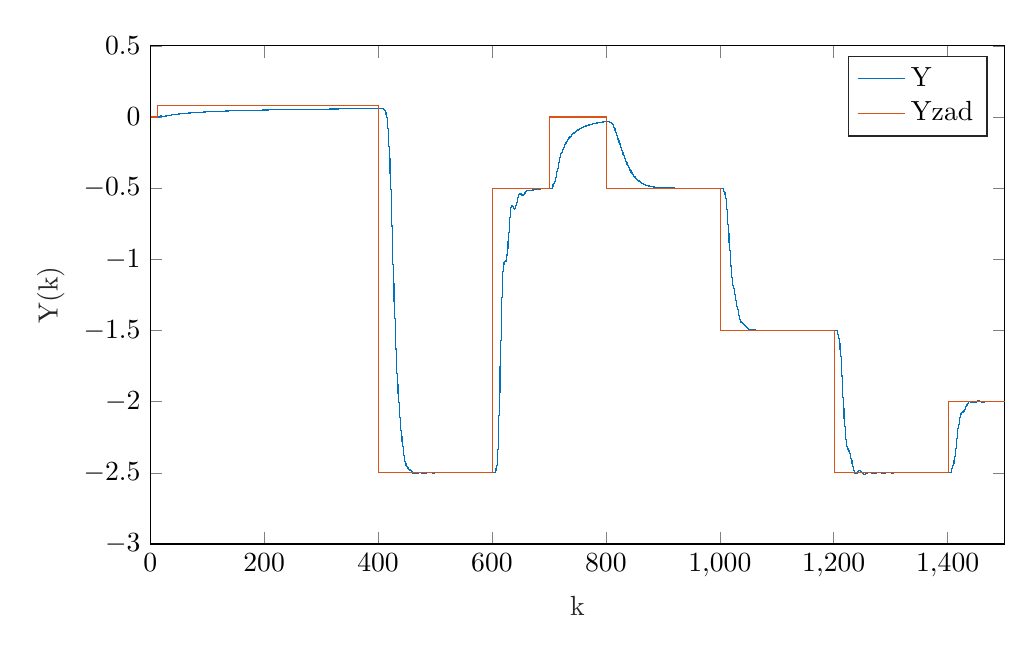
\begin{tikzpicture}

\begin{axis}[%
width=4.272in,
height=2.491in,
at={(0.717in,0.423in)},
scale only axis,
xmin=0,
xmax=1500,
xlabel style={font=\color{white!15!black}},
xlabel={k},
ymin=-3,
ymax=0.5,
ylabel style={font=\color{white!15!black}},
ylabel={Y(k)},
axis background/.style={fill=white},
legend style={legend cell align=left, align=left, draw=white!15!black}
]
\addplot[const plot, color=mycolor1] table[row sep=crcr] {%
1	0\\
2	0\\
3	0\\
4	0\\
5	0\\
6	0\\
7	0\\
8	0\\
9	0\\
10	0\\
11	0\\
12	0\\
13	0\\
14	0\\
15	0\\
16	0\\
17	0.00334251881758044\\
18	0.00679061482163346\\
19	0.00691360309366431\\
20	0.0059839446988958\\
21	0.00510374685954133\\
22	0.00448449104446296\\
23	0.0041170963650504\\
24	0.00422682851516356\\
25	0.00484724445370416\\
26	0.00575252736411783\\
27	0.00673968339852246\\
28	0.00770045361008513\\
29	0.00858347504822724\\
30	0.00936703504643653\\
31	0.0100629835484678\\
32	0.0107040734229228\\
33	0.0113212499334452\\
34	0.0119335931259751\\
35	0.0125491520828582\\
36	0.0131682141878489\\
37	0.0137862247316973\\
38	0.0143970259810856\\
39	0.0149955723711474\\
40	0.0155790809386762\\
41	0.0161468760804471\\
42	0.0166997025849788\\
43	0.0172389839459964\\
44	0.0177662112772462\\
45	0.0182825674133586\\
46	0.0187888089578147\\
47	0.0192853302343985\\
48	0.0197723017627876\\
49	0.0202498062149731\\
50	0.0207179349381671\\
51	0.0211768354542765\\
52	0.0216267177688158\\
53	0.0220678363537662\\
54	0.0225004647052943\\
55	0.0229248736968453\\
56	0.0233413184303013\\
57	0.0237500335908872\\
58	0.0241512348290726\\
59	0.0245451230354273\\
60	0.0249318889496757\\
61	0.0253117166456431\\
62	0.0256847854636602\\
63	0.0260512706280001\\
64	0.0264113430639514\\
65	0.0267651689220058\\
66	0.0271129091604572\\
67	0.0274547193488467\\
68	0.027790749706609\\
69	0.0281211453102434\\
70	0.0284460463808059\\
71	0.0287655885792605\\
72	0.0290799032675068\\
73	0.0293891177215184\\
74	0.0296933553020139\\
75	0.0299927355962722\\
76	0.030287374544831\\
77	0.0305773845627755\\
78	0.0308628746603921\\
79	0.0311439505640892\\
80	0.0314207148363297\\
81	0.0316932669926972\\
82	0.0319617036145592\\
83	0.0322261184565056\\
84	0.0324866025484247\\
85	0.0327432442925247\\
86	0.0329961295558011\\
87	0.0332453417584491\\
88	0.0334909619586178\\
89	0.0337330689337874\\
90	0.0339717392589472\\
91	0.0342070473817018\\
92	0.0344390656944061\\
93	0.0346678646034309\\
94	0.0348935125956686\\
95	0.0351160763023962\\
96	0.0353356205606166\\
97	0.0355522084719965\\
98	0.0357659014595152\\
99	0.035976759321929\\
100	0.0361848402861513\\
101	0.0363902010576406\\
102	0.0365928968688823\\
103	0.0367929815260474\\
104	0.0369905074539059\\
105	0.03718552573907\\
106	0.0373780861716373\\
107	0.0375682372853036\\
108	0.0377560263960093\\
109	0.0379414996391803\\
110	0.0381247020056246\\
111	0.038305677376138\\
112	0.0384844685548735\\
113	0.0386611173015259\\
114	0.0388356643623782\\
115	0.0390081495002579\\
116	0.0391786115234464\\
117	0.0393470883135833\\
118	0.0395136168526071\\
119	0.0396782332487688\\
120	0.039840972761757\\
121	0.040001869826968\\
122	0.0401609580789558\\
123	0.0403182703740916\\
124	0.0404738388124671\\
125	0.0406276947590667\\
126	0.0407798688642398\\
127	0.0409303910834982\\
128	0.0410792906966648\\
129	0.0412265963263979\\
130	0.0413723359561152\\
131	0.0415165369473386\\
132	0.0416592260564826\\
133	0.0418004294511067\\
134	0.0419401727256508\\
135	0.0420784809166733\\
136	0.0422153785176097\\
137	0.0423508894930694\\
138	0.0424850372926867\\
139	0.0426178448645429\\
140	0.0427493346681739\\
141	0.0428795286871794\\
142	0.0430084484414458\\
143	0.0431361149989986\\
144	0.0432625489874955\\
145	0.0433877706053743\\
146	0.0435117996326657\\
147	0.0436346554414849\\
148	0.0437563570062112\\
149	0.0438769229133666\\
150	0.0439963713712047\\
151	0.0441147202190187\\
152	0.0442319869361783\\
153	0.0443481886509048\\
154	0.0444633421487924\\
155	0.0445774638810859\\
156	0.0446905699727205\\
157	0.0448026762301337\\
158	0.0449137981488553\\
159	0.0450239509208838\\
160	0.0451331494418552\\
161	0.0452414083180122\\
162	0.0453487418729784\\
163	0.0454551641543462\\
164	0.0455606889400816\\
165	0.0456653297447544\\
166	0.0457690998255973\\
167	0.0458720121884004\\
168	0.0459740795932461\\
169	0.046075314560089\\
170	0.046175729374186\\
171	0.0462753360913814\\
172	0.0463741465432511\\
173	0.0464721723421101\\
174	0.0465694248858886\\
175	0.0466659153628787\\
176	0.0467616547563581\\
177	0.0468566538490924\\
178	0.0469509232277209\\
179	0.0470444732870288\\
180	0.0471373142341096\\
181	0.0472294560924208\\
182	0.047320908705736\\
183	0.0474116817419963\\
184	0.0475017846970646\\
185	0.047591226898385\\
186	0.0476800175085501\\
187	0.0477681655287796\\
188	0.0478556798023117\\
189	0.0479425690177107\\
190	0.0480288417120926\\
191	0.0481145062742716\\
192	0.0481995709478294\\
193	0.0482840438341091\\
194	0.0483679328951371\\
195	0.0484512459564737\\
196	0.0485339907099946\\
197	0.0486161747166067\\
198	0.0486978054088972\\
199	0.0487788900937213\\
200	0.0488594359547271\\
201	0.0489394500548213\\
202	0.0490189393385767\\
203	0.0490979106345834\\
204	0.0491763706577442\\
205	0.0492543260115179\\
206	0.0493317831901087\\
207	0.0494087485806068\\
208	0.0494852284650785\\
209	0.0495612290226082\\
210	0.0496367563312949\\
211	0.049711816370202\\
212	0.0497864150212633\\
213	0.0498605580711461\\
214	0.0499342512130717\\
215	0.0500075000485959\\
216	0.0500803100893486\\
217	0.050152686758736\\
218	0.0502246353936034\\
219	0.0502961612458625\\
220	0.0503672694840824\\
221	0.0504379651950451\\
222	0.0505082533852682\\
223	0.0505781389824928\\
224	0.0506476268371405\\
225	0.0507167217237379\\
226	0.050785428342311\\
227	0.0508537513197489\\
228	0.050921695211139\\
229	0.0509892645010732\\
230	0.0510564636049265\\
231	0.0511232968701085\\
232	0.0511897685772884\\
233	0.0512558829415939\\
234	0.0513216441137858\\
235	0.0513870561814068\\
236	0.0514521231699074\\
237	0.0515168490437481\\
238	0.0515812377074782\\
239	0.0516452930067933\\
240	0.0517090187295704\\
241	0.0517724186068817\\
242	0.0518354963139883\\
243	0.0518982554713131\\
244	0.0519606996453942\\
245	0.0520228323498188\\
246	0.0520846570461387\\
247	0.0521461771447668\\
248	0.052207396005856\\
249	0.0522683169401609\\
250	0.0523289432098814\\
251	0.0523892780294903\\
252	0.0524493245665446\\
253	0.05250908594248\\
254	0.0525685652333911\\
255	0.0526277654707946\\
256	0.0526866896423793\\
257	0.0527453406927403\\
258	0.0528037215240996\\
259	0.0528618349970126\\
260	0.0529196839310604\\
261	0.05297727110553\\
262	0.0530345992600804\\
263	0.0530916710953961\\
264	0.0531484892738289\\
265	0.0532050564200266\\
266	0.0532613751215504\\
267	0.0533174479294801\\
268	0.0533732773590086\\
269	0.0534288658900247\\
270	0.0534842159676852\\
271	0.0535393300029761\\
272	0.053594210373264\\
273	0.0536488594228362\\
274	0.053703279463432\\
275	0.0537574727747634\\
276	0.0538114416050263\\
277	0.0538651881714027\\
278	0.0539187146605535\\
279	0.0539720232291024\\
280	0.0540251160041106\\
281	0.0540779950835434\\
282	0.0541306625367285\\
283	0.0541831204048052\\
284	0.0542353707011665\\
285	0.0542874154118923\\
286	0.0543392564961762\\
287	0.054390895886743\\
288	0.0544423354902602\\
289	0.0544935771877418\\
290	0.054544622834944\\
291	0.0545954742627559\\
292	0.0546461332775812\\
293	0.0546966016617147\\
294	0.0547468811737115\\
295	0.0547969735487502\\
296	0.0548468804989894\\
297	0.0548966037139178\\
298	0.0549461448606993\\
299	0.054995505584511\\
300	0.0550446875088759\\
301	0.0550936922359897\\
302	0.0551425213470424\\
303	0.0551911764025339\\
304	0.0552396589425846\\
305	0.0552879704872402\\
306	0.0553361125367723\\
307	0.0553840865719727\\
308	0.055431894054444\\
309	0.0554795364268838\\
310	0.055527015113366\\
311	0.0555743315196155\\
312	0.0556214870332797\\
313	0.055668483024195\\
314	0.0557153208446484\\
315	0.0557620018296357\\
316	0.0558085272971145\\
317	0.0558548985482539\\
318	0.0559011168676794\\
319	0.0559471835237138\\
320	0.055993099768615\\
321	0.0560388668388087\\
322	0.0560844859551181\\
323	0.0561299583229899\\
324	0.0561752851327159\\
325	0.056220467559652\\
326	0.0562655067644329\\
327	0.0563104038931835\\
328	0.0563551600777274\\
329	0.0563997764357912\\
330	0.0564442540712064\\
331	0.0564885940741073\\
332	0.0565327975211263\\
333	0.056576865475586\\
334	0.0566207989876878\\
335	0.0566645990946982\\
336	0.0567082668211318\\
337	0.0567518031789312\\
338	0.0567952091676445\\
339	0.0568384857745997\\
340	0.0568816339750765\\
341	0.0569246547324756\\
342	0.0569675489984849\\
343	0.0570103177132435\\
344	0.0570529618055028\\
345	0.0570954821927857\\
346	0.0571378797815428\\
347	0.0571801554673061\\
348	0.0572223101348408\\
349	0.0572643446582949\\
350	0.0573062599013451\\
351	0.0573480567173429\\
352	0.0573897359494558\\
353	0.0574312984308084\\
354	0.0574727449846205\\
355	0.0575140764243427\\
356	0.057555293553791\\
357	0.0575963971672784\\
358	0.0576373880497451\\
359	0.0576782669768864\\
360	0.0577190347152787\\
361	0.0577596920225041\\
362	0.0578002396472722\\
363	0.0578406783295412\\
364	0.0578810088006361\\
365	0.057921231783366\\
366	0.0579613479921389\\
367	0.0580013581330756\\
368	0.0580412629041213\\
369	0.0580810629951558\\
370	0.0581207590881019\\
371	0.0581603518570325\\
372	0.0581998419682758\\
373	0.0582392300805192\\
374	0.0582785168449114\\
375	0.0583177029051634\\
376	0.0583567888976475\\
377	0.0583957754514954\\
378	0.0584346631886947\\
379	0.0584734527241834\\
380	0.0585121446659441\\
381	0.0585507396150962\\
382	0.0585892381659863\\
383	0.0586276409062786\\
384	0.0586659484170426\\
385	0.0587041612728404\\
386	0.0587422800418127\\
387	0.0587803052857629\\
388	0.0588182375602411\\
389	0.0588560774146255\\
390	0.058893825392204\\
391	0.0589314820302537\\
392	0.0589690478601199\\
393	0.0590065234072933\\
394	0.0590439091914867\\
395	0.0590812057267104\\
396	0.0591184135213462\\
397	0.0591555330782213\\
398	0.0591925648946799\\
399	0.0592295094626547\\
400	0.059266367268737\\
401	0.0593031387942462\\
402	0.0593398245152976\\
403	0.0593764249028701\\
404	0.0594129404228722\\
405	0.0594493715362078\\
406	0.0595428978937022\\
407	0.0581554981489647\\
408	0.0584370640160367\\
409	0.0575487942049385\\
410	0.0550628082061132\\
411	0.05075414577074\\
412	0.0440043058994822\\
413	0.0336698353685206\\
414	0.018117950603272\\
415	-0.00463968930191905\\
416	-0.0367479105686905\\
417	-0.0802894497949369\\
418	-0.13709845251169\\
419	-0.208607643128808\\
420	-0.295257116550392\\
421	-0.396342235161168\\
422	-0.510194113594916\\
423	-0.634364752407965\\
424	-0.765806815970501\\
425	-0.901134025444611\\
426	-1.03692704996772\\
427	-1.16999832463507\\
428	-1.297600704765\\
429	-1.41758867826774\\
430	-1.52851800939796\\
431	-1.62966698584179\\
432	-1.72098392432322\\
433	-1.80297667743022\\
434	-1.87655997971402\\
435	-1.94287975120071\\
436	-2.00313812989824\\
437	-2.05844135817911\\
438	-2.10968606992315\\
439	-2.1574925793754\\
440	-2.20218724020893\\
441	-2.2438294417162\\
442	-2.2822734790508\\
443	-2.31725243629129\\
444	-2.34847017078658\\
445	-2.37568799660424\\
446	-2.3987945917727\\
447	-2.41785083535585\\
448	-2.43310528458227\\
449	-2.44498030648665\\
450	-2.45403296870376\\
451	-2.46089811976494\\
452	-2.46622313791437\\
453	-2.47060430550143\\
454	-2.47453369632304\\
455	-2.47836315277597\\
456	-2.48228887291706\\
457	-2.48635688661007\\
458	-2.49048678276785\\
459	-2.49450882526309\\
460	-2.49820826739213\\
461	-2.5013702993809\\
462	-2.50381957839399\\
463	-2.50544954593012\\
464	-2.50623851896342\\
465	-2.50625158905143\\
466	-2.50562939433976\\
467	-2.50456656599601\\
468	-2.5032838622782\\
469	-2.50199854509141\\
470	-2.50089739255179\\
471	-2.50011595892913\\
472	-2.4997264653363\\
473	-2.49973525796125\\
474	-2.50008933920678\\
475	-2.50069026187386\\
476	-2.50141282083777\\
477	-2.50212555616302\\
478	-2.50271010604735\\
479	-2.50307687023216\\
480	-2.50317517292506\\
481	-2.50299702681746\\
482	-2.50257455957932\\
483	-2.50197203662837\\
484	-2.50127408416251\\
485	-2.50057210510642\\
486	-2.49995095463268\\
487	-2.49947771717781\\
488	-2.49919396247349\\
489	-2.49911224324294\\
490	-2.49921693412676\\
491	-2.49946889832752\\
492	-2.49981298565371\\
493	-2.50018706641153\\
494	-2.50053121257209\\
495	-2.50079574363064\\
496	-2.50094712679149\\
497	-2.50097110782995\\
498	-2.50087288763349\\
499	-2.50067458544282\\
500	-2.5004105853182\\
501	-2.50012160367903\\
502	-2.49984841873047\\
503	-2.499626164689\\
504	-2.49947993283895\\
505	-2.49942217152112\\
506	-2.49945208164496\\
507	-2.49955690894389\\
508	-2.49971478010425\\
509	-2.49989854836277\\
510	-2.50008002333433\\
511	-2.50023396367448\\
512	-2.50034130042494\\
513	-2.50039121353236\\
514	-2.50038187697173\\
515	-2.50031988917171\\
516	-2.50021858645932\\
517	-2.50009557465467\\
518	-2.49996989243633\\
519	-2.49985923391781\\
520	-2.49977761087708\\
521	-2.49973373934249\\
522	-2.49973030860343\\
523	-2.49976415370484\\
524	-2.49982722514016\\
525	-2.49990814856495\\
526	-2.49999410443478\\
527	-2.50007273771766\\
528	-2.50013383000557\\
529	-2.50017052356921\\
530	-2.50017996809175\\
531	-2.50016335259996\\
532	-2.50012537382825\\
533	-2.50007326587121\\
534	-2.50001556562184\\
535	-2.49996080939829\\
536	-2.49991634800439\\
537	-2.49988743401219\\
538	-2.49987668325899\\
539	-2.49988395130039\\
540	-2.49990660424046\\
541	-2.49994011049527\\
542	-2.49997884219624\\
543	-2.50001695597603\\
544	-2.50004922370332\\
545	-2.50007170242597\\
546	-2.50008216513443\\
547	-2.50008025425148\\
548	-2.50006736168774\\
549	-2.5000462769112\\
550	-2.50002067293211\\
551	-2.49999451627405\\
552	-2.49997148975116\\
553	-2.49995450703107\\
554	-2.49994537804478\\
555	-2.49994465799285\\
556	-2.4999516842315\\
557	-2.49996477885204\\
558	-2.49998157378575\\
559	-2.49999940218448\\
560	-2.500015695739\\
561	-2.50002833225169\\
562	-2.50003588973733\\
563	-2.50003778026521\\
564	-2.50003425587665\\
565	-2.50002629736416\\
566	-2.50001541198092\\
567	-2.50000337642804\\
568	-2.499991965766\\
569	-2.49998270716238\\
570	-2.49997669040674\\
571	-2.49997445634317\\
572	-2.4999759716327\\
573	-2.4999806855097\\
574	-2.49998765320878\\
575	-2.49999570287616\\
576	-2.50000361884982\\
577	-2.50001031438266\\
578	-2.5000149707923\\
579	-2.50001712677028\\
580	-2.50001670997737\\
581	-2.50001401177721\\
582	-2.50000961377645\\
583	-2.50000428074297\\
584	-2.49999883781867\\
585	-2.49999405049777\\
586	-2.49999052378055\\
587	-2.49998863276112\\
588	-2.49998849143052\\
589	-2.49998996055647\\
590	-2.49999268999791\\
591	-2.49999618645455\\
592	-2.49999989493801\\
593	-2.50000328141001\\
594	-2.50000590501091\\
595	-2.50000747079754\\
596	-2.50000785743899\\
597	-2.50000711829894\\
598	-2.50000545817001\\
599	-2.50000319109969\\
600	-2.50000068687862\\
601	-2.49999831464866\\
602	-2.49999639172009\\
603	-2.49999514423013\\
604	-2.49999468402886\\
605	-2.49999500352793\\
606	-2.48493160869072\\
607	-2.47118421063002\\
608	-2.45056960597041\\
609	-2.40824688431497\\
610	-2.33500374615547\\
611	-2.23097069998372\\
612	-2.09543329937107\\
613	-1.93211529818194\\
614	-1.75267170414176\\
615	-1.57289869260103\\
616	-1.406953858366\\
617	-1.26608919933642\\
618	-1.15746676946816\\
619	-1.08294161661944\\
620	-1.03925707486328\\
621	-1.01953938709121\\
622	-1.0148135672676\\
623	-1.01534940792318\\
624	-1.01210640185295\\
625	-0.998162990235502\\
626	-0.969766220952567\\
627	-0.926810124159627\\
628	-0.872630062861501\\
629	-0.813030299613816\\
630	-0.754745725237008\\
631	-0.703857616618903\\
632	-0.664641215101728\\
633	-0.639021217152802\\
634	-0.626571045788505\\
635	-0.624910595064921\\
636	-0.630354372342113\\
637	-0.638674007018461\\
638	-0.645855874048196\\
639	-0.648752510224465\\
640	-0.64553873877688\\
641	-0.635898919016436\\
642	-0.620910834081581\\
643	-0.602659582587565\\
644	-0.583687233672893\\
645	-0.566423152926408\\
646	-0.552725732273184\\
647	-0.543612379395438\\
648	-0.539193483907299\\
649	-0.538781715456907\\
650	-0.541125069758353\\
651	-0.544704346023023\\
652	-0.5480369540606\\
653	-0.54993597573105\\
654	-0.549685180700967\\
655	-0.547107144957388\\
656	-0.542522180225882\\
657	-0.536617459968054\\
658	-0.530262961472159\\
659	-0.524318264746535\\
660	-0.519470084783196\\
661	-0.516127461001399\\
662	-0.514385121298437\\
663	-0.51405057439449\\
664	-0.514719726942318\\
665	-0.515879983448114\\
666	-0.517018442451508\\
667	-0.517715156676214\\
668	-0.517706618010179\\
669	-0.516911707267238\\
670	-0.515420136541218\\
671	-0.513450498005229\\
672	-0.511290026495231\\
673	-0.509230151853245\\
674	-0.507510736093149\\
675	-0.506282258223656\\
676	-0.505590323163495\\
677	-0.505381976456285\\
678	-0.505529358415163\\
679	-0.505863764574727\\
680	-0.506212342773807\\
681	-0.506430312821384\\
682	-0.506423410515485\\
683	-0.506157776691955\\
684	-0.505657212735949\\
685	-0.504990095273457\\
686	-0.504249872964206\\
687	-0.503533728455918\\
688	-0.502923674291597\\
689	-0.502473263473933\\
690	-0.50220156534315\\
691	-0.502094451937573\\
692	-0.502111875266055\\
693	-0.50219890520073\\
694	-0.502297933804622\\
695	-0.502359615750356\\
696	-0.502350698697471\\
697	-0.502257737387168\\
698	-0.502086592969362\\
699	-0.501858418216742\\
700	-0.501603385198413\\
701	-0.501353653073813\\
702	-0.501136998311578\\
703	-0.500972197776997\\
704	-0.500866767600122\\
705	-0.500817132901538\\
706	-0.486751847911068\\
707	-0.4758998896861\\
708	-0.469359810562358\\
709	-0.462123479386276\\
710	-0.451385946197444\\
711	-0.439094947332868\\
712	-0.424585733206213\\
713	-0.406543464455013\\
714	-0.385548907060663\\
715	-0.363343950545167\\
716	-0.341170330450716\\
717	-0.320023035387597\\
718	-0.300917819794266\\
719	-0.284478725840333\\
720	-0.270690096537947\\
721	-0.259128265562588\\
722	-0.249196992029959\\
723	-0.240227571277687\\
724	-0.231602308534422\\
725	-0.222900582874226\\
726	-0.213956335050134\\
727	-0.204822678095073\\
728	-0.195702097006669\\
729	-0.18686572697421\\
730	-0.178568987886935\\
731	-0.170985886708692\\
732	-0.164179816039544\\
733	-0.158108613483391\\
734	-0.152652305263613\\
735	-0.14765250613693\\
736	-0.14295270345725\\
737	-0.138429394306413\\
738	-0.134008312481886\\
739	-0.129665456341061\\
740	-0.12541638054392\\
741	-0.121299028886574\\
742	-0.117355749705242\\
743	-0.113619078732703\\
744	-0.110103791246549\\
745	-0.106805506378262\\
746	-0.103704458790105\\
747	-0.100772166760458\\
748	-0.0979786034901624\\
749	-0.0952979733750691\\
750	-0.0927120394729617\\
751	-0.0902108346259486\\
752	-0.0877912803331423\\
753	-0.0854546150744126\\
754	-0.0832035856536054\\
755	-0.0810401529491356\\
756	-0.0789641269088081\\
757	-0.0769727980812648\\
758	-0.07506136603879\\
759	-0.0732238235312213\\
760	-0.0714539395491138\\
761	-0.0697460631019936\\
762	-0.068095595671191\\
763	-0.0664991082945295\\
764	-0.0649541760019516\\
765	-0.0634590522796458\\
766	-0.0620123103192298\\
767	-0.0606125484572909\\
768	-0.0592582118466216\\
769	-0.057947537420517\\
770	-0.0566785960234337\\
771	-0.0554493891297531\\
772	-0.0542579569958276\\
773	-0.0531024656936308\\
774	-0.0519812561061933\\
775	-0.0508928530587521\\
776	-0.0498359436004218\\
777	-0.0488093385733963\\
778	-0.0478119314805443\\
779	-0.0468426649712605\\
780	-0.0459005100890994\\
781	-0.0449844585721146\\
782	-0.0440935251196734\\
783	-0.0432267550395841\\
784	-0.042383232851973\\
785	-0.0415620886732331\\
786	-0.0407625008603703\\
787	-0.039983694900337\\
788	-0.0392249395401944\\
789	-0.0384855415713559\\
790	-0.03776484059185\\
791	-0.0370622046652156\\
792	-0.0363770272837056\\
793	-0.0357087255952809\\
794	-0.0350567395644694\\
795	-0.0344205316290466\\
796	-0.0337995864551556\\
797	-0.0331934105223529\\
798	-0.0326015314237937\\
799	-0.032023496896868\\
800	-0.0314588736801601\\
801	-0.0309072463195154\\
802	-0.0303682160306308\\
803	-0.0298413996865172\\
804	-0.0293264289538776\\
805	-0.0288229495663814\\
806	-0.0338628182889581\\
807	-0.0377696673522113\\
808	-0.0385160356039966\\
809	-0.0396553892138882\\
810	-0.0426883564685413\\
811	-0.0474322529792925\\
812	-0.0538038483184986\\
813	-0.0621333328027087\\
814	-0.0721935988242601\\
815	-0.0833639711030645\\
816	-0.0951418666918442\\
817	-0.107209726554096\\
818	-0.119306761617887\\
819	-0.131255664938632\\
820	-0.143020967503994\\
821	-0.154663248562758\\
822	-0.166267021953743\\
823	-0.177910842291402\\
824	-0.189653967990263\\
825	-0.201517573918561\\
826	-0.21347609358656\\
827	-0.225466278553465\\
828	-0.237402763364045\\
829	-0.249192302947294\\
830	-0.260747030056738\\
831	-0.271995846960675\\
832	-0.282890864532157\\
833	-0.293408153057902\\
834	-0.303544446408294\\
835	-0.31331138778457\\
836	-0.322728526716381\\
837	-0.331816519966751\\
838	-0.340591885612233\\
839	-0.349063980547557\\
840	-0.357234245021742\\
841	-0.365097401736678\\
842	-0.372644031923854\\
843	-0.379863767929277\\
844	-0.386748350887292\\
845	-0.393293977549148\\
846	-0.399502597680416\\
847	-0.405382068123539\\
848	-0.410945296970711\\
849	-0.416208681899337\\
850	-0.421190229336979\\
851	-0.425907736457884\\
852	-0.430377345658903\\
853	-0.434612664537291\\
854	-0.438624510163812\\
855	-0.442421212688638\\
856	-0.446009321854886\\
857	-0.449394511987725\\
858	-0.452582477930253\\
859	-0.455579649861559\\
860	-0.458393616563061\\
861	-0.461033219002479\\
862	-0.463508344076422\\
863	-0.465829500208488\\
864	-0.468007285187348\\
865	-0.47005186038293\\
866	-0.471972527420192\\
867	-0.473777470215219\\
868	-0.475473685441295\\
869	-0.477067086374921\\
870	-0.478562735465247\\
871	-0.47996514406726\\
872	-0.481278574789605\\
873	-0.482507291291633\\
874	-0.483655718531356\\
875	-0.484728498743245\\
876	-0.485730450076382\\
877	-0.486666451933673\\
878	-0.487541291129064\\
879	-0.488359505202655\\
880	-0.489125254361033\\
881	-0.489842243503074\\
882	-0.490513703271947\\
883	-0.491142426740719\\
884	-0.491730848455214\\
885	-0.492281146596956\\
886	-0.492795347518547\\
887	-0.493275414467878\\
888	-0.493723307879635\\
889	-0.494141011698722\\
890	-0.494530527270608\\
891	-0.494893842077595\\
892	-0.495232884145983\\
893	-0.495549473961665\\
894	-0.495845284395411\\
895	-0.496121816047752\\
896	-0.496380391409771\\
897	-0.496622167181859\\
898	-0.496848160757501\\
899	-0.497059284777812\\
900	-0.4972563830047\\
901	-0.497440261456753\\
902	-0.497611710474482\\
903	-0.497771515659646\\
904	-0.497920457962162\\
905	-0.498059305127028\\
906	-0.498188797959194\\
907	-0.498309635286305\\
908	-0.498422461139568\\
909	-0.49852785671297\\
910	-0.498626338367015\\
911	-0.498718361604505\\
912	-0.498804329818174\\
913	-0.498884605871974\\
914	-0.498959524309737\\
915	-0.499029402167925\\
916	-0.499094546903116\\
917	-0.499155260679128\\
918	-0.49921184102731\\
919	-0.499264578548481\\
920	-0.499313752760928\\
921	-0.499359627366737\\
922	-0.499402446116277\\
923	-0.499442430153164\\
924	-0.499479777304703\\
925	-0.499514663340738\\
926	-0.499547244842848\\
927	-0.499577663067834\\
928	-0.499606048084389\\
929	-0.499632522507002\\
930	-0.499657204315985\\
931	-0.499680208489015\\
932	-0.499701647423096\\
933	-0.499721630346848\\
934	-0.499740262074929\\
935	-0.499757641521195\\
936	-0.499773860365371\\
937	-0.499789002176322\\
938	-0.499803142160683\\
939	-0.499816347559814\\
940	-0.499828678589582\\
941	-0.499840189727714\\
942	-0.499850931113352\\
943	-0.499860949833318\\
944	-0.499870290920142\\
945	-0.499878997962926\\
946	-0.499887113315582\\
947	-0.499894677961415\\
948	-0.499901731145715\\
949	-0.499908309912503\\
950	-0.499914448677251\\
951	-0.49992017893935\\
952	-0.499925529194992\\
953	-0.499930525063125\\
954	-0.499935189593958\\
955	-0.499939543698339\\
956	-0.499943606621396\\
957	-0.499947396385324\\
958	-0.499950930141657\\
959	-0.499954224397654\\
960	-0.499957295108898\\
961	-0.499960157655197\\
962	-0.499962826735082\\
963	-0.499965316223307\\
964	-0.499967639035247\\
965	-0.499969807033641\\
966	-0.499971830999301\\
967	-0.499973720671644\\
968	-0.499975484850434\\
969	-0.499977131539335\\
970	-0.49997866810641\\
971	-0.499980101436601\\
972	-0.499981438055892\\
973	-0.499982684214631\\
974	-0.499983845926444\\
975	-0.499984928967617\\
976	-0.499985938848024\\
977	-0.499986880768061\\
978	-0.499987759576178\\
979	-0.499988579739069\\
980	-0.499989345332175\\
981	-0.499990060053006\\
982	-0.4999907272549\\
983	-0.499991349995184\\
984	-0.499991931089674\\
985	-0.499992473165229\\
986	-0.499992978703495\\
987	-0.499993450071409\\
988	-0.499993889536997\\
989	-0.499994299271788\\
990	-0.499994681343328\\
991	-0.499995037702479\\
992	-0.499995370170347\\
993	-0.499995680428927\\
994	-0.499995970018162\\
995	-0.499996240340436\\
996	-0.499996492671866\\
997	-0.499996728178526\\
998	-0.499996947934997\\
999	-0.499997152942518\\
1000	-0.499997344144387\\
1001	-0.499997522437092\\
1002	-0.499997688676572\\
1003	-0.499997843679951\\
1004	-0.499997988223846\\
1005	-0.499998123040744\\
1006	-0.512413672821433\\
1007	-0.522498491218511\\
1008	-0.531925401523103\\
1009	-0.547614532538056\\
1010	-0.573007989312179\\
1011	-0.606905676639375\\
1012	-0.64935641276156\\
1013	-0.700406603481834\\
1014	-0.758113938655403\\
1015	-0.819332175027629\\
1016	-0.881180240915086\\
1017	-0.941122244113117\\
1018	-0.996822956037993\\
1019	-1.04655274567451\\
1020	-1.08953126267405\\
1021	-1.12583538299286\\
1022	-1.1561887178693\\
1023	-1.18180929113245\\
1024	-1.20419703338883\\
1025	-1.22484675090276\\
1026	-1.24500809429106\\
1027	-1.26554420278547\\
1028	-1.28686411242554\\
1029	-1.30892100851737\\
1030	-1.33128309715713\\
1031	-1.35325938432504\\
1032	-1.37404767598935\\
1033	-1.39288055462296\\
1034	-1.40915240326191\\
1035	-1.42251082036964\\
1036	-1.43290022632929\\
1037	-1.44055527431122\\
1038	-1.44595015482223\\
1039	-1.44971535733981\\
1040	-1.45253752570268\\
1041	-1.45505991973214\\
1042	-1.45779924355189\\
1043	-1.46108999432016\\
1044	-1.46506179928748\\
1045	-1.46964955863746\\
1046	-1.4746312790139\\
1047	-1.47968493785684\\
1048	-1.48445393413518\\
1049	-1.48861058442255\\
1050	-1.49190845456499\\
1051	-1.49421679146385\\
1052	-1.49553356452632\\
1053	-1.49597714965748\\
1054	-1.49575995303467\\
1055	-1.49514978472362\\
1056	-1.49442618319283\\
1057	-1.49383899612901\\
1058	-1.49357543004105\\
1059	-1.49373980247345\\
1060	-1.49434780289908\\
1061	-1.49533464291627\\
1062	-1.49657443227102\\
1063	-1.4979067112676\\
1064	-1.49916542404754\\
1065	-1.50020573086953\\
1066	-1.50092483265514\\
1067	-1.50127424551586\\
1068	-1.5012624944776\\
1069	-1.50094874873125\\
1070	-1.50042925921741\\
1071	-1.49981939168682\\
1072	-1.4992344594012\\
1073	-1.49877242890635\\
1074	-1.49850097257632\\
1075	-1.49845041750061\\
1076	-1.49861307394397\\
1077	-1.4989484008273\\
1078	-1.49939263321495\\
1079	-1.49987096106176\\
1080	-1.50031015601676\\
1081	-1.50064968550885\\
1082	-1.50084977564167\\
1083	-1.50089549726929\\
1084	-1.50079664420263\\
1085	-1.5005838368732\\
1086	-1.50030182031138\\
1087	-1.50000126093843\\
1088	-1.49973044861372\\
1089	-1.49952818495507\\
1090	-1.49941882823963\\
1091	-1.49941003656152\\
1092	-1.49949328316282\\
1093	-1.49964678709695\\
1094	-1.49984017043138\\
1095	-1.50003995988468\\
1096	-1.50021501078676\\
1097	-1.50034103489734\\
1098	-1.50040363100761\\
1099	-1.50039950454077\\
1100	-1.50033586940705\\
1101	-1.50022830360435\\
1102	-1.50009753969715\\
1103	-1.49996578671746\\
1104	-1.49985319254354\\
1105	-1.49977497359614\\
1106	-1.49973958387868\\
1107	-1.49974809915612\\
1108	-1.4997947887816\\
1109	-1.49986866917095\\
1110	-1.49995570387238\\
1111	-1.50004125014664\\
1112	-1.50011235433709\\
1113	-1.50015956094211\\
1114	-1.5001780077174\\
1115	-1.50016771061238\\
1116	-1.50013307552665\\
1117	-1.50008178828315\\
1118	-1.50002331419974\\
1119	-1.49996727532458\\
1120	-1.49992196542449\\
1121	-1.49989321583239\\
1122	-1.49988375037047\\
1123	-1.49989307904494\\
1124	-1.49991789297401\\
1125	-1.49995285025755\\
1126	-1.49999159386128\\
1127	-1.5000278230513\\
1128	-1.50005624953216\\
1129	-1.50007330384037\\
1130	-1.50007750902454\\
1131	-1.50006949766993\\
1132	-1.50005170515319\\
1133	-1.50002781818448\\
1134	-1.50000208720791\\
1135	-1.49997862122229\\
1136	-1.49996077446159\\
1137	-1.49995070943584\\
1138	-1.49994918547204\\
1139	-1.49995558255835\\
1140	-1.49996813339286\\
1141	-1.49998430745957\\
1142	-1.50000127335252\\
1143	-1.5000163609809\\
1144	-1.50002745311309\\
1145	-1.50003325352642\\
1146	-1.50003340311301\\
1147	-1.50002844135374\\
1148	-1.50001963443759\\
1149	-1.50000870954863\\
1150	-1.49999754523597\\
1151	-1.49998786951851\\
1152	-1.49998101104936\\
1153	-1.49997773604628\\
1154	-1.49997818733891\\
1155	-1.49998192466252\\
1156	-1.49998804995757\\
1157	-1.49999539007645\\
1158	-1.50000270328582\\
1159	-1.50000887566959\\
1160	-1.5000130784553\\
1161	-1.50001486613804\\
1162	-1.50001420631765\\
1163	-1.50001144349466\\
1164	-1.50000720892973\\
1165	-1.50000229570095\\
1166	-1.49999752150165\\
1167	-1.49999360134778\\
1168	-1.49999104864251\\
1169	-1.49999011687791\\
1170	-1.49999078682561\\
1171	-1.4999927966401\\
1172	-1.49999570600328\\
1173	-1.49999898112633\\
1174	-1.50000208555403\\
1175	-1.50000456233084\\
1176	-1.50000609584516\\
1177	-1.50000654593429\\
1178	-1.50000595180622\\
1179	-1.50000450818598\\
1180	-1.50000252009487\\
1181	-1.50000034529506\\
1182	-1.4999983344154\\
1183	-1.49999677813079\\
1184	-1.4999958687567\\
1185	-1.49999568068631\\
1186	-1.49999617077987\\
1187	-1.49999719665906\\
1188	-1.49999854832976\\
1189	-1.49999998697755\\
1190	-1.50000128429859\\
1191	-1.50000225630794\\
1192	-1.50000278701395\\
1193	-1.50000283935373\\
1194	-1.50000245298918\\
1195	-1.50000173060892\\
1196	-1.50000081597221\\
1197	-1.49999986786977\\
1198	-1.49999903438358\\
1199	-1.49999843134574\\
1200	-1.49999812786679\\
1201	-1.49999814043875\\
1202	-1.4999984356589\\
1203	-1.4999989402997\\
1204	-1.49999955645569\\
1205	-1.50000017894911\\
1206	-1.5137011107264\\
1207	-1.52606226392196\\
1208	-1.53854992322007\\
1209	-1.55849643147522\\
1210	-1.58998408750998\\
1211	-1.63196614053981\\
1212	-1.68453502654749\\
1213	-1.74773880148145\\
1214	-1.81936587832434\\
1215	-1.89563138991327\\
1216	-1.97279100913435\\
1217	-2.04733956969547\\
1218	-2.11591852196684\\
1219	-2.17581661827396\\
1220	-2.22546270571881\\
1221	-2.26445458159445\\
1222	-2.29341183931112\\
1223	-2.3138475675711\\
1224	-2.3279336483507\\
1225	-2.3381286012551\\
1226	-2.34680424679956\\
1227	-2.3559553299553\\
1228	-2.36699141389125\\
1229	-2.38061985023246\\
1230	-2.39684110201615\\
1231	-2.41504676961859\\
1232	-2.4341865052107\\
1233	-2.45297270265525\\
1234	-2.47009675854925\\
1235	-2.48442873385645\\
1236	-2.49517427425972\\
1237	-2.50197142458207\\
1238	-2.50491946415113\\
1239	-2.5045403146655\\
1240	-2.50168213832174\\
1241	-2.49738328821809\\
1242	-2.4927198457641\\
1243	-2.48866050919993\\
1244	-2.48594926946791\\
1245	-2.48503012027832\\
1246	-2.48602025632538\\
1247	-2.48873043991792\\
1248	-2.49272481558289\\
1249	-2.49740806767957\\
1250	-2.50212556962566\\
1251	-2.50626195646841\\
1252	-2.50932511595036\\
1253	-2.51100558180177\\
1254	-2.51120531637736\\
1255	-2.51003441846046\\
1256	-2.50777882126041\\
1257	-2.50484592410943\\
1258	-2.50169774908976\\
1259	-2.49878224769858\\
1260	-2.49647272149314\\
1261	-2.49502320617456\\
1262	-2.49454459167306\\
1263	-2.49500281337084\\
1264	-2.49623722037574\\
1265	-2.49799464098784\\
1266	-2.49997298473957\\
1267	-2.50186754018501\\
1268	-2.50341340966241\\
1269	-2.50441862998487\\
1270	-2.50478425408619\\
1271	-2.50450975437696\\
1272	-2.50368426330934\\
1273	-2.50246609581659\\
1274	-2.50105444223617\\
1275	-2.4996578972177\\
1276	-2.49846452952292\\
1277	-2.49761755190651\\
1278	-2.49719947850872\\
1279	-2.49722618672604\\
1280	-2.49765077865219\\
1281	-2.49837578695213\\
1282	-2.4992712595281\\
1283	-2.50019568525304\\
1284	-2.50101661795331\\
1285	-2.50162818416357\\
1286	-2.50196333853003\\
1287	-2.50199963993\\
1288	-2.50175832196164\\
1289	-2.50129738083539\\
1290	-2.5007001743529\\
1291	-2.50006152250784\\
1292	-2.49947347377858\\
1293	-2.49901275317926\\
1294	-2.49873148821389\\
1295	-2.49865220275039\\
1296	-2.49876738120717\\
1297	-2.49904324172965\\
1298	-2.49942680752626\\
1299	-2.49985499448535\\
1300	-2.50026427345974\\
1301	-2.50059951830609\\
1302	-2.50082088886791\\
1303	-2.50090797267827\\
1304	-2.50086085748566\\
1305	-2.50069826120914\\
1306	-2.50045324339163\\
1307	-2.50016731209297\\
1308	-2.49988389087999\\
1309	-2.49964211286072\\
1310	-2.49947177534898\\
1311	-2.49939005086902\\
1312	-2.49940025104694\\
1313	-2.49949262726803\\
1314	-2.49964691074832\\
1315	-2.49983608090102\\
1316	-2.50003072765786\\
1317	-2.50020334913358\\
1318	-2.50033199483567\\
1319	-2.50040280858621\\
1320	-2.50041121793071\\
1321	-2.50036172724321\\
1322	-2.50026646936515\\
1323	-2.50014282914596\\
1324	-2.50001055304208\\
1325	-2.49988879299587\\
1326	-2.49979350133724\\
1327	-2.49973550674438\\
1328	-2.49971947653199\\
1329	-2.49974382863968\\
1330	-2.49980151903035\\
1331	-2.49988151551971\\
1332	-2.49997069110557\\
1333	-2.50005583602872\\
1334	-2.50012549868806\\
1335	-2.5001714155589\\
1336	-2.50018936897251\\
1337	-2.50017940554748\\
1338	-2.50014544285771\\
1339	-2.50009437435966\\
1340	-2.50003484233609\\
1341	-2.4999758793674\\
1342	-2.49992561893372\\
1343	-2.49989024793588\\
1344	-2.49987332460933\\
1345	-2.4998755233195\\
1346	-2.49989480285541\\
1347	-2.49992693635997\\
1348	-2.49996629648163\\
1349	-2.5000067636024\\
1350	-2.5000426199341\\
1351	-2.5000693066938\\
1352	-2.50008395170376\\
1353	-2.50008561501399\\
1354	-2.50007524402559\\
1355	-2.50005537068784\\
1356	-2.50002961619974\\
1357	-2.50000208944487\\
1358	-2.499976772326\\
1359	-2.49995697853026\\
1360	-2.49994495420129\\
1361	-2.49994166306843\\
1362	-2.49994676910581\\
1363	-2.49995880118426\\
1364	-2.49997546033054\\
1365	-2.49999401399563\\
1366	-2.50001171471005\\
1367	-2.50002618280661\\
1368	-2.5000357033527\\
1369	-2.50003940386373\\
1370	-2.50003729894801\\
1371	-2.50003020775987\\
1372	-2.50001956726068\\
1373	-2.5000071766664\\
1374	-2.49999491480381\\
1375	-2.4999844720731\\
1376	-2.49997713290107\\
1377	-2.49997363430092\\
1378	-2.49997411326257\\
1379	-2.49997814220991\\
1380	-2.49998483960619\\
1381	-2.49999303353131\\
1382	-2.50000145071628\\
1383	-2.50000890248536\\
1384	-2.50001444207719\\
1385	-2.50001747410597\\
1386	-2.5000178053125\\
1387	-2.50001563488878\\
1388	-2.50001149120343\\
1389	-2.50000612857607\\
1390	-2.50000040205646\\
1391	-2.49999513958775\\
1392	-2.49999102953751\\
1393	-2.49998853781403\\
1394	-2.49998786338742\\
1395	-2.49998893490318\\
1396	-2.49999144512722\\
1397	-2.49999491500662\\
1398	-2.49999877576491\\
1399	-2.5000024559994\\
1400	-2.50000546123656\\
1401	-2.5000074355872\\
1402	-2.50000819856795\\
1403	-2.50000775423198\\
1404	-2.50000627385496\\
1405	-2.50000405698006\\
1406	-2.4849370688367\\
1407	-2.47118570652299\\
1408	-2.46054305994023\\
1409	-2.44819391948848\\
1410	-2.43105273452258\\
1411	-2.4111007899673\\
1412	-2.3879480550401\\
1413	-2.36012460525665\\
1414	-2.32788945709833\\
1415	-2.29298055069736\\
1416	-2.25690831476009\\
1417	-2.22111640817202\\
1418	-2.18737910638139\\
1419	-2.15735880722685\\
1420	-2.1320987423948\\
1421	-2.1120393702476\\
1422	-2.09712945818571\\
1423	-2.08681604333302\\
1424	-2.0801081232237\\
1425	-2.07578068452273\\
1426	-2.07258263931871\\
1427	-2.06938856278581\\
1428	-2.0653260473848\\
1429	-2.05987532379159\\
1430	-2.05290527344024\\
1431	-2.0446414362323\\
1432	-2.03558770994582\\
1433	-2.02641826819067\\
1434	-2.01785296101336\\
1435	-2.01053659053236\\
1436	-2.00494265022736\\
1437	-2.00131327311357\\
1438	-1.99963914959509\\
1439	-1.9996782059372\\
1440	-2.00100680993318\\
1441	-2.00309270807652\\
1442	-2.00537692869433\\
1443	-2.00735231431231\\
1444	-2.00862801099474\\
1445	-2.00897192044796\\
1446	-2.00832683208895\\
1447	-2.00680011814086\\
1448	-2.00463072905043\\
1449	-2.0021402548991\\
1450	-1.99967665330318\\
1451	-1.9975596153582\\
1452	-1.99603545511267\\
1453	-1.99524719765147\\
1454	-1.99522270940548\\
1455	-1.99588077972438\\
1456	-1.99705247729801\\
1457	-1.99851320001367\\
1458	-2.00001978846174\\
1459	-2.00134691249385\\
1460	-2.00231758794515\\
1461	-2.00282397650186\\
1462	-2.00283634312833\\
1463	-2.00239992926799\\
1464	-2.00162127174001\\
1465	-2.00064690680466\\
1466	-1.99963825901667\\
1467	-1.99874673343073\\
1468	-1.99809262614707\\
1469	-1.99775056181379\\
1470	-1.99774294744937\\
1471	-1.99804161799484\\
1472	-1.99857664585971\\
1473	-1.99925035637938\\
1474	-1.99995403515365\\
1475	-2.00058466889009\\
1476	-2.00105930653622\\
1477	-2.0013251911721\\
1478	-2.00136458887882\\
1479	-2.00119410209382\\
1480	-2.0008590723649\\
1481	-2.00042433622646\\
1482	-1.99996301430989\\
1483	-1.99954514628679\\
1484	-1.99922783793256\\
1485	-1.99904820901143\\
1486	-1.99901990031877\\
1487	-1.99913330875538\\
1488	-1.99935916317107\\
1489	-1.99965460816313\\
1490	-1.99997068077255\\
1491	-2.0002599699258\\
1492	-2.0004833357113\\
1493	-2.00061480551537\\
1494	-2.00064410859485\\
1495	-2.00057670135073\\
1496	-2.00043151226984\\
1497	-2.00023694499631\\
1498	-2.00002588113978\\
1499	-1.99983050095496\\
1500	-1.99967769017478\\
};
\addlegendentry{Y}

\addplot[const plot, color=mycolor2] table[row sep=crcr] {%
1	0\\
2	0\\
3	0\\
4	0\\
5	0\\
6	0\\
7	0\\
8	0\\
9	0\\
10	0\\
11	0\\
12	0.08\\
13	0.08\\
14	0.08\\
15	0.08\\
16	0.08\\
17	0.08\\
18	0.08\\
19	0.08\\
20	0.08\\
21	0.08\\
22	0.08\\
23	0.08\\
24	0.08\\
25	0.08\\
26	0.08\\
27	0.08\\
28	0.08\\
29	0.08\\
30	0.08\\
31	0.08\\
32	0.08\\
33	0.08\\
34	0.08\\
35	0.08\\
36	0.08\\
37	0.08\\
38	0.08\\
39	0.08\\
40	0.08\\
41	0.08\\
42	0.08\\
43	0.08\\
44	0.08\\
45	0.08\\
46	0.08\\
47	0.08\\
48	0.08\\
49	0.08\\
50	0.08\\
51	0.08\\
52	0.08\\
53	0.08\\
54	0.08\\
55	0.08\\
56	0.08\\
57	0.08\\
58	0.08\\
59	0.08\\
60	0.08\\
61	0.08\\
62	0.08\\
63	0.08\\
64	0.08\\
65	0.08\\
66	0.08\\
67	0.08\\
68	0.08\\
69	0.08\\
70	0.08\\
71	0.08\\
72	0.08\\
73	0.08\\
74	0.08\\
75	0.08\\
76	0.08\\
77	0.08\\
78	0.08\\
79	0.08\\
80	0.08\\
81	0.08\\
82	0.08\\
83	0.08\\
84	0.08\\
85	0.08\\
86	0.08\\
87	0.08\\
88	0.08\\
89	0.08\\
90	0.08\\
91	0.08\\
92	0.08\\
93	0.08\\
94	0.08\\
95	0.08\\
96	0.08\\
97	0.08\\
98	0.08\\
99	0.08\\
100	0.08\\
101	0.08\\
102	0.08\\
103	0.08\\
104	0.08\\
105	0.08\\
106	0.08\\
107	0.08\\
108	0.08\\
109	0.08\\
110	0.08\\
111	0.08\\
112	0.08\\
113	0.08\\
114	0.08\\
115	0.08\\
116	0.08\\
117	0.08\\
118	0.08\\
119	0.08\\
120	0.08\\
121	0.08\\
122	0.08\\
123	0.08\\
124	0.08\\
125	0.08\\
126	0.08\\
127	0.08\\
128	0.08\\
129	0.08\\
130	0.08\\
131	0.08\\
132	0.08\\
133	0.08\\
134	0.08\\
135	0.08\\
136	0.08\\
137	0.08\\
138	0.08\\
139	0.08\\
140	0.08\\
141	0.08\\
142	0.08\\
143	0.08\\
144	0.08\\
145	0.08\\
146	0.08\\
147	0.08\\
148	0.08\\
149	0.08\\
150	0.08\\
151	0.08\\
152	0.08\\
153	0.08\\
154	0.08\\
155	0.08\\
156	0.08\\
157	0.08\\
158	0.08\\
159	0.08\\
160	0.08\\
161	0.08\\
162	0.08\\
163	0.08\\
164	0.08\\
165	0.08\\
166	0.08\\
167	0.08\\
168	0.08\\
169	0.08\\
170	0.08\\
171	0.08\\
172	0.08\\
173	0.08\\
174	0.08\\
175	0.08\\
176	0.08\\
177	0.08\\
178	0.08\\
179	0.08\\
180	0.08\\
181	0.08\\
182	0.08\\
183	0.08\\
184	0.08\\
185	0.08\\
186	0.08\\
187	0.08\\
188	0.08\\
189	0.08\\
190	0.08\\
191	0.08\\
192	0.08\\
193	0.08\\
194	0.08\\
195	0.08\\
196	0.08\\
197	0.08\\
198	0.08\\
199	0.08\\
200	0.08\\
201	0.08\\
202	0.08\\
203	0.08\\
204	0.08\\
205	0.08\\
206	0.08\\
207	0.08\\
208	0.08\\
209	0.08\\
210	0.08\\
211	0.08\\
212	0.08\\
213	0.08\\
214	0.08\\
215	0.08\\
216	0.08\\
217	0.08\\
218	0.08\\
219	0.08\\
220	0.08\\
221	0.08\\
222	0.08\\
223	0.08\\
224	0.08\\
225	0.08\\
226	0.08\\
227	0.08\\
228	0.08\\
229	0.08\\
230	0.08\\
231	0.08\\
232	0.08\\
233	0.08\\
234	0.08\\
235	0.08\\
236	0.08\\
237	0.08\\
238	0.08\\
239	0.08\\
240	0.08\\
241	0.08\\
242	0.08\\
243	0.08\\
244	0.08\\
245	0.08\\
246	0.08\\
247	0.08\\
248	0.08\\
249	0.08\\
250	0.08\\
251	0.08\\
252	0.08\\
253	0.08\\
254	0.08\\
255	0.08\\
256	0.08\\
257	0.08\\
258	0.08\\
259	0.08\\
260	0.08\\
261	0.08\\
262	0.08\\
263	0.08\\
264	0.08\\
265	0.08\\
266	0.08\\
267	0.08\\
268	0.08\\
269	0.08\\
270	0.08\\
271	0.08\\
272	0.08\\
273	0.08\\
274	0.08\\
275	0.08\\
276	0.08\\
277	0.08\\
278	0.08\\
279	0.08\\
280	0.08\\
281	0.08\\
282	0.08\\
283	0.08\\
284	0.08\\
285	0.08\\
286	0.08\\
287	0.08\\
288	0.08\\
289	0.08\\
290	0.08\\
291	0.08\\
292	0.08\\
293	0.08\\
294	0.08\\
295	0.08\\
296	0.08\\
297	0.08\\
298	0.08\\
299	0.08\\
300	0.08\\
301	0.08\\
302	0.08\\
303	0.08\\
304	0.08\\
305	0.08\\
306	0.08\\
307	0.08\\
308	0.08\\
309	0.08\\
310	0.08\\
311	0.08\\
312	0.08\\
313	0.08\\
314	0.08\\
315	0.08\\
316	0.08\\
317	0.08\\
318	0.08\\
319	0.08\\
320	0.08\\
321	0.08\\
322	0.08\\
323	0.08\\
324	0.08\\
325	0.08\\
326	0.08\\
327	0.08\\
328	0.08\\
329	0.08\\
330	0.08\\
331	0.08\\
332	0.08\\
333	0.08\\
334	0.08\\
335	0.08\\
336	0.08\\
337	0.08\\
338	0.08\\
339	0.08\\
340	0.08\\
341	0.08\\
342	0.08\\
343	0.08\\
344	0.08\\
345	0.08\\
346	0.08\\
347	0.08\\
348	0.08\\
349	0.08\\
350	0.08\\
351	0.08\\
352	0.08\\
353	0.08\\
354	0.08\\
355	0.08\\
356	0.08\\
357	0.08\\
358	0.08\\
359	0.08\\
360	0.08\\
361	0.08\\
362	0.08\\
363	0.08\\
364	0.08\\
365	0.08\\
366	0.08\\
367	0.08\\
368	0.08\\
369	0.08\\
370	0.08\\
371	0.08\\
372	0.08\\
373	0.08\\
374	0.08\\
375	0.08\\
376	0.08\\
377	0.08\\
378	0.08\\
379	0.08\\
380	0.08\\
381	0.08\\
382	0.08\\
383	0.08\\
384	0.08\\
385	0.08\\
386	0.08\\
387	0.08\\
388	0.08\\
389	0.08\\
390	0.08\\
391	0.08\\
392	0.08\\
393	0.08\\
394	0.08\\
395	0.08\\
396	0.08\\
397	0.08\\
398	0.08\\
399	0.08\\
400	0.08\\
401	-2.5\\
402	-2.5\\
403	-2.5\\
404	-2.5\\
405	-2.5\\
406	-2.5\\
407	-2.5\\
408	-2.5\\
409	-2.5\\
410	-2.5\\
411	-2.5\\
412	-2.5\\
413	-2.5\\
414	-2.5\\
415	-2.5\\
416	-2.5\\
417	-2.5\\
418	-2.5\\
419	-2.5\\
420	-2.5\\
421	-2.5\\
422	-2.5\\
423	-2.5\\
424	-2.5\\
425	-2.5\\
426	-2.5\\
427	-2.5\\
428	-2.5\\
429	-2.5\\
430	-2.5\\
431	-2.5\\
432	-2.5\\
433	-2.5\\
434	-2.5\\
435	-2.5\\
436	-2.5\\
437	-2.5\\
438	-2.5\\
439	-2.5\\
440	-2.5\\
441	-2.5\\
442	-2.5\\
443	-2.5\\
444	-2.5\\
445	-2.5\\
446	-2.5\\
447	-2.5\\
448	-2.5\\
449	-2.5\\
450	-2.5\\
451	-2.5\\
452	-2.5\\
453	-2.5\\
454	-2.5\\
455	-2.5\\
456	-2.5\\
457	-2.5\\
458	-2.5\\
459	-2.5\\
460	-2.5\\
461	-2.5\\
462	-2.5\\
463	-2.5\\
464	-2.5\\
465	-2.5\\
466	-2.5\\
467	-2.5\\
468	-2.5\\
469	-2.5\\
470	-2.5\\
471	-2.5\\
472	-2.5\\
473	-2.5\\
474	-2.5\\
475	-2.5\\
476	-2.5\\
477	-2.5\\
478	-2.5\\
479	-2.5\\
480	-2.5\\
481	-2.5\\
482	-2.5\\
483	-2.5\\
484	-2.5\\
485	-2.5\\
486	-2.5\\
487	-2.5\\
488	-2.5\\
489	-2.5\\
490	-2.5\\
491	-2.5\\
492	-2.5\\
493	-2.5\\
494	-2.5\\
495	-2.5\\
496	-2.5\\
497	-2.5\\
498	-2.5\\
499	-2.5\\
500	-2.5\\
501	-2.5\\
502	-2.5\\
503	-2.5\\
504	-2.5\\
505	-2.5\\
506	-2.5\\
507	-2.5\\
508	-2.5\\
509	-2.5\\
510	-2.5\\
511	-2.5\\
512	-2.5\\
513	-2.5\\
514	-2.5\\
515	-2.5\\
516	-2.5\\
517	-2.5\\
518	-2.5\\
519	-2.5\\
520	-2.5\\
521	-2.5\\
522	-2.5\\
523	-2.5\\
524	-2.5\\
525	-2.5\\
526	-2.5\\
527	-2.5\\
528	-2.5\\
529	-2.5\\
530	-2.5\\
531	-2.5\\
532	-2.5\\
533	-2.5\\
534	-2.5\\
535	-2.5\\
536	-2.5\\
537	-2.5\\
538	-2.5\\
539	-2.5\\
540	-2.5\\
541	-2.5\\
542	-2.5\\
543	-2.5\\
544	-2.5\\
545	-2.5\\
546	-2.5\\
547	-2.5\\
548	-2.5\\
549	-2.5\\
550	-2.5\\
551	-2.5\\
552	-2.5\\
553	-2.5\\
554	-2.5\\
555	-2.5\\
556	-2.5\\
557	-2.5\\
558	-2.5\\
559	-2.5\\
560	-2.5\\
561	-2.5\\
562	-2.5\\
563	-2.5\\
564	-2.5\\
565	-2.5\\
566	-2.5\\
567	-2.5\\
568	-2.5\\
569	-2.5\\
570	-2.5\\
571	-2.5\\
572	-2.5\\
573	-2.5\\
574	-2.5\\
575	-2.5\\
576	-2.5\\
577	-2.5\\
578	-2.5\\
579	-2.5\\
580	-2.5\\
581	-2.5\\
582	-2.5\\
583	-2.5\\
584	-2.5\\
585	-2.5\\
586	-2.5\\
587	-2.5\\
588	-2.5\\
589	-2.5\\
590	-2.5\\
591	-2.5\\
592	-2.5\\
593	-2.5\\
594	-2.5\\
595	-2.5\\
596	-2.5\\
597	-2.5\\
598	-2.5\\
599	-2.5\\
600	-2.5\\
601	-0.5\\
602	-0.5\\
603	-0.5\\
604	-0.5\\
605	-0.5\\
606	-0.5\\
607	-0.5\\
608	-0.5\\
609	-0.5\\
610	-0.5\\
611	-0.5\\
612	-0.5\\
613	-0.5\\
614	-0.5\\
615	-0.5\\
616	-0.5\\
617	-0.5\\
618	-0.5\\
619	-0.5\\
620	-0.5\\
621	-0.5\\
622	-0.5\\
623	-0.5\\
624	-0.5\\
625	-0.5\\
626	-0.5\\
627	-0.5\\
628	-0.5\\
629	-0.5\\
630	-0.5\\
631	-0.5\\
632	-0.5\\
633	-0.5\\
634	-0.5\\
635	-0.5\\
636	-0.5\\
637	-0.5\\
638	-0.5\\
639	-0.5\\
640	-0.5\\
641	-0.5\\
642	-0.5\\
643	-0.5\\
644	-0.5\\
645	-0.5\\
646	-0.5\\
647	-0.5\\
648	-0.5\\
649	-0.5\\
650	-0.5\\
651	-0.5\\
652	-0.5\\
653	-0.5\\
654	-0.5\\
655	-0.5\\
656	-0.5\\
657	-0.5\\
658	-0.5\\
659	-0.5\\
660	-0.5\\
661	-0.5\\
662	-0.5\\
663	-0.5\\
664	-0.5\\
665	-0.5\\
666	-0.5\\
667	-0.5\\
668	-0.5\\
669	-0.5\\
670	-0.5\\
671	-0.5\\
672	-0.5\\
673	-0.5\\
674	-0.5\\
675	-0.5\\
676	-0.5\\
677	-0.5\\
678	-0.5\\
679	-0.5\\
680	-0.5\\
681	-0.5\\
682	-0.5\\
683	-0.5\\
684	-0.5\\
685	-0.5\\
686	-0.5\\
687	-0.5\\
688	-0.5\\
689	-0.5\\
690	-0.5\\
691	-0.5\\
692	-0.5\\
693	-0.5\\
694	-0.5\\
695	-0.5\\
696	-0.5\\
697	-0.5\\
698	-0.5\\
699	-0.5\\
700	-0.5\\
701	0\\
702	0\\
703	0\\
704	0\\
705	0\\
706	0\\
707	0\\
708	0\\
709	0\\
710	0\\
711	0\\
712	0\\
713	0\\
714	0\\
715	0\\
716	0\\
717	0\\
718	0\\
719	0\\
720	0\\
721	0\\
722	0\\
723	0\\
724	0\\
725	0\\
726	0\\
727	0\\
728	0\\
729	0\\
730	0\\
731	0\\
732	0\\
733	0\\
734	0\\
735	0\\
736	0\\
737	0\\
738	0\\
739	0\\
740	0\\
741	0\\
742	0\\
743	0\\
744	0\\
745	0\\
746	0\\
747	0\\
748	0\\
749	0\\
750	0\\
751	0\\
752	0\\
753	0\\
754	0\\
755	0\\
756	0\\
757	0\\
758	0\\
759	0\\
760	0\\
761	0\\
762	0\\
763	0\\
764	0\\
765	0\\
766	0\\
767	0\\
768	0\\
769	0\\
770	0\\
771	0\\
772	0\\
773	0\\
774	0\\
775	0\\
776	0\\
777	0\\
778	0\\
779	0\\
780	0\\
781	0\\
782	0\\
783	0\\
784	0\\
785	0\\
786	0\\
787	0\\
788	0\\
789	0\\
790	0\\
791	0\\
792	0\\
793	0\\
794	0\\
795	0\\
796	0\\
797	0\\
798	0\\
799	0\\
800	0\\
801	-0.5\\
802	-0.5\\
803	-0.5\\
804	-0.5\\
805	-0.5\\
806	-0.5\\
807	-0.5\\
808	-0.5\\
809	-0.5\\
810	-0.5\\
811	-0.5\\
812	-0.5\\
813	-0.5\\
814	-0.5\\
815	-0.5\\
816	-0.5\\
817	-0.5\\
818	-0.5\\
819	-0.5\\
820	-0.5\\
821	-0.5\\
822	-0.5\\
823	-0.5\\
824	-0.5\\
825	-0.5\\
826	-0.5\\
827	-0.5\\
828	-0.5\\
829	-0.5\\
830	-0.5\\
831	-0.5\\
832	-0.5\\
833	-0.5\\
834	-0.5\\
835	-0.5\\
836	-0.5\\
837	-0.5\\
838	-0.5\\
839	-0.5\\
840	-0.5\\
841	-0.5\\
842	-0.5\\
843	-0.5\\
844	-0.5\\
845	-0.5\\
846	-0.5\\
847	-0.5\\
848	-0.5\\
849	-0.5\\
850	-0.5\\
851	-0.5\\
852	-0.5\\
853	-0.5\\
854	-0.5\\
855	-0.5\\
856	-0.5\\
857	-0.5\\
858	-0.5\\
859	-0.5\\
860	-0.5\\
861	-0.5\\
862	-0.5\\
863	-0.5\\
864	-0.5\\
865	-0.5\\
866	-0.5\\
867	-0.5\\
868	-0.5\\
869	-0.5\\
870	-0.5\\
871	-0.5\\
872	-0.5\\
873	-0.5\\
874	-0.5\\
875	-0.5\\
876	-0.5\\
877	-0.5\\
878	-0.5\\
879	-0.5\\
880	-0.5\\
881	-0.5\\
882	-0.5\\
883	-0.5\\
884	-0.5\\
885	-0.5\\
886	-0.5\\
887	-0.5\\
888	-0.5\\
889	-0.5\\
890	-0.5\\
891	-0.5\\
892	-0.5\\
893	-0.5\\
894	-0.5\\
895	-0.5\\
896	-0.5\\
897	-0.5\\
898	-0.5\\
899	-0.5\\
900	-0.5\\
901	-0.5\\
902	-0.5\\
903	-0.5\\
904	-0.5\\
905	-0.5\\
906	-0.5\\
907	-0.5\\
908	-0.5\\
909	-0.5\\
910	-0.5\\
911	-0.5\\
912	-0.5\\
913	-0.5\\
914	-0.5\\
915	-0.5\\
916	-0.5\\
917	-0.5\\
918	-0.5\\
919	-0.5\\
920	-0.5\\
921	-0.5\\
922	-0.5\\
923	-0.5\\
924	-0.5\\
925	-0.5\\
926	-0.5\\
927	-0.5\\
928	-0.5\\
929	-0.5\\
930	-0.5\\
931	-0.5\\
932	-0.5\\
933	-0.5\\
934	-0.5\\
935	-0.5\\
936	-0.5\\
937	-0.5\\
938	-0.5\\
939	-0.5\\
940	-0.5\\
941	-0.5\\
942	-0.5\\
943	-0.5\\
944	-0.5\\
945	-0.5\\
946	-0.5\\
947	-0.5\\
948	-0.5\\
949	-0.5\\
950	-0.5\\
951	-0.5\\
952	-0.5\\
953	-0.5\\
954	-0.5\\
955	-0.5\\
956	-0.5\\
957	-0.5\\
958	-0.5\\
959	-0.5\\
960	-0.5\\
961	-0.5\\
962	-0.5\\
963	-0.5\\
964	-0.5\\
965	-0.5\\
966	-0.5\\
967	-0.5\\
968	-0.5\\
969	-0.5\\
970	-0.5\\
971	-0.5\\
972	-0.5\\
973	-0.5\\
974	-0.5\\
975	-0.5\\
976	-0.5\\
977	-0.5\\
978	-0.5\\
979	-0.5\\
980	-0.5\\
981	-0.5\\
982	-0.5\\
983	-0.5\\
984	-0.5\\
985	-0.5\\
986	-0.5\\
987	-0.5\\
988	-0.5\\
989	-0.5\\
990	-0.5\\
991	-0.5\\
992	-0.5\\
993	-0.5\\
994	-0.5\\
995	-0.5\\
996	-0.5\\
997	-0.5\\
998	-0.5\\
999	-0.5\\
1000	-0.5\\
1001	-1.5\\
1002	-1.5\\
1003	-1.5\\
1004	-1.5\\
1005	-1.5\\
1006	-1.5\\
1007	-1.5\\
1008	-1.5\\
1009	-1.5\\
1010	-1.5\\
1011	-1.5\\
1012	-1.5\\
1013	-1.5\\
1014	-1.5\\
1015	-1.5\\
1016	-1.5\\
1017	-1.5\\
1018	-1.5\\
1019	-1.5\\
1020	-1.5\\
1021	-1.5\\
1022	-1.5\\
1023	-1.5\\
1024	-1.5\\
1025	-1.5\\
1026	-1.5\\
1027	-1.5\\
1028	-1.5\\
1029	-1.5\\
1030	-1.5\\
1031	-1.5\\
1032	-1.5\\
1033	-1.5\\
1034	-1.5\\
1035	-1.5\\
1036	-1.5\\
1037	-1.5\\
1038	-1.5\\
1039	-1.5\\
1040	-1.5\\
1041	-1.5\\
1042	-1.5\\
1043	-1.5\\
1044	-1.5\\
1045	-1.5\\
1046	-1.5\\
1047	-1.5\\
1048	-1.5\\
1049	-1.5\\
1050	-1.5\\
1051	-1.5\\
1052	-1.5\\
1053	-1.5\\
1054	-1.5\\
1055	-1.5\\
1056	-1.5\\
1057	-1.5\\
1058	-1.5\\
1059	-1.5\\
1060	-1.5\\
1061	-1.5\\
1062	-1.5\\
1063	-1.5\\
1064	-1.5\\
1065	-1.5\\
1066	-1.5\\
1067	-1.5\\
1068	-1.5\\
1069	-1.5\\
1070	-1.5\\
1071	-1.5\\
1072	-1.5\\
1073	-1.5\\
1074	-1.5\\
1075	-1.5\\
1076	-1.5\\
1077	-1.5\\
1078	-1.5\\
1079	-1.5\\
1080	-1.5\\
1081	-1.5\\
1082	-1.5\\
1083	-1.5\\
1084	-1.5\\
1085	-1.5\\
1086	-1.5\\
1087	-1.5\\
1088	-1.5\\
1089	-1.5\\
1090	-1.5\\
1091	-1.5\\
1092	-1.5\\
1093	-1.5\\
1094	-1.5\\
1095	-1.5\\
1096	-1.5\\
1097	-1.5\\
1098	-1.5\\
1099	-1.5\\
1100	-1.5\\
1101	-1.5\\
1102	-1.5\\
1103	-1.5\\
1104	-1.5\\
1105	-1.5\\
1106	-1.5\\
1107	-1.5\\
1108	-1.5\\
1109	-1.5\\
1110	-1.5\\
1111	-1.5\\
1112	-1.5\\
1113	-1.5\\
1114	-1.5\\
1115	-1.5\\
1116	-1.5\\
1117	-1.5\\
1118	-1.5\\
1119	-1.5\\
1120	-1.5\\
1121	-1.5\\
1122	-1.5\\
1123	-1.5\\
1124	-1.5\\
1125	-1.5\\
1126	-1.5\\
1127	-1.5\\
1128	-1.5\\
1129	-1.5\\
1130	-1.5\\
1131	-1.5\\
1132	-1.5\\
1133	-1.5\\
1134	-1.5\\
1135	-1.5\\
1136	-1.5\\
1137	-1.5\\
1138	-1.5\\
1139	-1.5\\
1140	-1.5\\
1141	-1.5\\
1142	-1.5\\
1143	-1.5\\
1144	-1.5\\
1145	-1.5\\
1146	-1.5\\
1147	-1.5\\
1148	-1.5\\
1149	-1.5\\
1150	-1.5\\
1151	-1.5\\
1152	-1.5\\
1153	-1.5\\
1154	-1.5\\
1155	-1.5\\
1156	-1.5\\
1157	-1.5\\
1158	-1.5\\
1159	-1.5\\
1160	-1.5\\
1161	-1.5\\
1162	-1.5\\
1163	-1.5\\
1164	-1.5\\
1165	-1.5\\
1166	-1.5\\
1167	-1.5\\
1168	-1.5\\
1169	-1.5\\
1170	-1.5\\
1171	-1.5\\
1172	-1.5\\
1173	-1.5\\
1174	-1.5\\
1175	-1.5\\
1176	-1.5\\
1177	-1.5\\
1178	-1.5\\
1179	-1.5\\
1180	-1.5\\
1181	-1.5\\
1182	-1.5\\
1183	-1.5\\
1184	-1.5\\
1185	-1.5\\
1186	-1.5\\
1187	-1.5\\
1188	-1.5\\
1189	-1.5\\
1190	-1.5\\
1191	-1.5\\
1192	-1.5\\
1193	-1.5\\
1194	-1.5\\
1195	-1.5\\
1196	-1.5\\
1197	-1.5\\
1198	-1.5\\
1199	-1.5\\
1200	-1.5\\
1201	-2.5\\
1202	-2.5\\
1203	-2.5\\
1204	-2.5\\
1205	-2.5\\
1206	-2.5\\
1207	-2.5\\
1208	-2.5\\
1209	-2.5\\
1210	-2.5\\
1211	-2.5\\
1212	-2.5\\
1213	-2.5\\
1214	-2.5\\
1215	-2.5\\
1216	-2.5\\
1217	-2.5\\
1218	-2.5\\
1219	-2.5\\
1220	-2.5\\
1221	-2.5\\
1222	-2.5\\
1223	-2.5\\
1224	-2.5\\
1225	-2.5\\
1226	-2.5\\
1227	-2.5\\
1228	-2.5\\
1229	-2.5\\
1230	-2.5\\
1231	-2.5\\
1232	-2.5\\
1233	-2.5\\
1234	-2.5\\
1235	-2.5\\
1236	-2.5\\
1237	-2.5\\
1238	-2.5\\
1239	-2.5\\
1240	-2.5\\
1241	-2.5\\
1242	-2.5\\
1243	-2.5\\
1244	-2.5\\
1245	-2.5\\
1246	-2.5\\
1247	-2.5\\
1248	-2.5\\
1249	-2.5\\
1250	-2.5\\
1251	-2.5\\
1252	-2.5\\
1253	-2.5\\
1254	-2.5\\
1255	-2.5\\
1256	-2.5\\
1257	-2.5\\
1258	-2.5\\
1259	-2.5\\
1260	-2.5\\
1261	-2.5\\
1262	-2.5\\
1263	-2.5\\
1264	-2.5\\
1265	-2.5\\
1266	-2.5\\
1267	-2.5\\
1268	-2.5\\
1269	-2.5\\
1270	-2.5\\
1271	-2.5\\
1272	-2.5\\
1273	-2.5\\
1274	-2.5\\
1275	-2.5\\
1276	-2.5\\
1277	-2.5\\
1278	-2.5\\
1279	-2.5\\
1280	-2.5\\
1281	-2.5\\
1282	-2.5\\
1283	-2.5\\
1284	-2.5\\
1285	-2.5\\
1286	-2.5\\
1287	-2.5\\
1288	-2.5\\
1289	-2.5\\
1290	-2.5\\
1291	-2.5\\
1292	-2.5\\
1293	-2.5\\
1294	-2.5\\
1295	-2.5\\
1296	-2.5\\
1297	-2.5\\
1298	-2.5\\
1299	-2.5\\
1300	-2.5\\
1301	-2.5\\
1302	-2.5\\
1303	-2.5\\
1304	-2.5\\
1305	-2.5\\
1306	-2.5\\
1307	-2.5\\
1308	-2.5\\
1309	-2.5\\
1310	-2.5\\
1311	-2.5\\
1312	-2.5\\
1313	-2.5\\
1314	-2.5\\
1315	-2.5\\
1316	-2.5\\
1317	-2.5\\
1318	-2.5\\
1319	-2.5\\
1320	-2.5\\
1321	-2.5\\
1322	-2.5\\
1323	-2.5\\
1324	-2.5\\
1325	-2.5\\
1326	-2.5\\
1327	-2.5\\
1328	-2.5\\
1329	-2.5\\
1330	-2.5\\
1331	-2.5\\
1332	-2.5\\
1333	-2.5\\
1334	-2.5\\
1335	-2.5\\
1336	-2.5\\
1337	-2.5\\
1338	-2.5\\
1339	-2.5\\
1340	-2.5\\
1341	-2.5\\
1342	-2.5\\
1343	-2.5\\
1344	-2.5\\
1345	-2.5\\
1346	-2.5\\
1347	-2.5\\
1348	-2.5\\
1349	-2.5\\
1350	-2.5\\
1351	-2.5\\
1352	-2.5\\
1353	-2.5\\
1354	-2.5\\
1355	-2.5\\
1356	-2.5\\
1357	-2.5\\
1358	-2.5\\
1359	-2.5\\
1360	-2.5\\
1361	-2.5\\
1362	-2.5\\
1363	-2.5\\
1364	-2.5\\
1365	-2.5\\
1366	-2.5\\
1367	-2.5\\
1368	-2.5\\
1369	-2.5\\
1370	-2.5\\
1371	-2.5\\
1372	-2.5\\
1373	-2.5\\
1374	-2.5\\
1375	-2.5\\
1376	-2.5\\
1377	-2.5\\
1378	-2.5\\
1379	-2.5\\
1380	-2.5\\
1381	-2.5\\
1382	-2.5\\
1383	-2.5\\
1384	-2.5\\
1385	-2.5\\
1386	-2.5\\
1387	-2.5\\
1388	-2.5\\
1389	-2.5\\
1390	-2.5\\
1391	-2.5\\
1392	-2.5\\
1393	-2.5\\
1394	-2.5\\
1395	-2.5\\
1396	-2.5\\
1397	-2.5\\
1398	-2.5\\
1399	-2.5\\
1400	-2.5\\
1401	-2\\
1402	-2\\
1403	-2\\
1404	-2\\
1405	-2\\
1406	-2\\
1407	-2\\
1408	-2\\
1409	-2\\
1410	-2\\
1411	-2\\
1412	-2\\
1413	-2\\
1414	-2\\
1415	-2\\
1416	-2\\
1417	-2\\
1418	-2\\
1419	-2\\
1420	-2\\
1421	-2\\
1422	-2\\
1423	-2\\
1424	-2\\
1425	-2\\
1426	-2\\
1427	-2\\
1428	-2\\
1429	-2\\
1430	-2\\
1431	-2\\
1432	-2\\
1433	-2\\
1434	-2\\
1435	-2\\
1436	-2\\
1437	-2\\
1438	-2\\
1439	-2\\
1440	-2\\
1441	-2\\
1442	-2\\
1443	-2\\
1444	-2\\
1445	-2\\
1446	-2\\
1447	-2\\
1448	-2\\
1449	-2\\
1450	-2\\
1451	-2\\
1452	-2\\
1453	-2\\
1454	-2\\
1455	-2\\
1456	-2\\
1457	-2\\
1458	-2\\
1459	-2\\
1460	-2\\
1461	-2\\
1462	-2\\
1463	-2\\
1464	-2\\
1465	-2\\
1466	-2\\
1467	-2\\
1468	-2\\
1469	-2\\
1470	-2\\
1471	-2\\
1472	-2\\
1473	-2\\
1474	-2\\
1475	-2\\
1476	-2\\
1477	-2\\
1478	-2\\
1479	-2\\
1480	-2\\
1481	-2\\
1482	-2\\
1483	-2\\
1484	-2\\
1485	-2\\
1486	-2\\
1487	-2\\
1488	-2\\
1489	-2\\
1490	-2\\
1491	-2\\
1492	-2\\
1493	-2\\
1494	-2\\
1495	-2\\
1496	-2\\
1497	-2\\
1498	-2\\
1499	-2\\
1500	-2\\
};
\addlegendentry{Yzad}

\end{axis}
\end{tikzpicture}%
\caption{Regulacja, $K = 0,3; T_i=4,5; T_d=1,54;$}
\end{figure}

\begin{figure}[H]
\centering
% This file was created by matlab2tikz.
%
%The latest updates can be retrieved from
%  http://www.mathworks.com/matlabcentral/fileexchange/22022-matlab2tikz-matlab2tikz
%where you can also make suggestions and rate matlab2tikz.
%
\definecolor{mycolor1}{rgb}{0.00000,0.44700,0.74100}%
%
\begin{tikzpicture}

\begin{axis}[%
width=4.272in,
height=2.491in,
at={(0.717in,0.423in)},
scale only axis,
xmin=0,
xmax=1500,
xlabel style={font=\color{white!15!black}},
xlabel={k},
ymin=-1.1,
ymax=1.1,
ylabel style={font=\color{white!15!black}},
ylabel={U(k)},
axis background/.style={fill=white}
]
\addplot[const plot, color=mycolor1, forget plot] table[row sep=crcr] {%
1	0\\
2	0\\
3	0\\
4	0\\
5	0\\
6	0\\
7	0\\
8	0\\
9	0\\
10	0\\
11	0\\
12	0.075\\
13	0.00374666666666663\\
14	0.00641333333333327\\
15	0.00907999999999991\\
16	0.0117466666666665\\
17	0.0102663816536551\\
18	0.0116321806381516\\
19	0.0171059467356758\\
20	0.0208091973110196\\
21	0.0235094269169827\\
22	0.025960955932675\\
23	0.0283617615236516\\
24	0.0304155779401323\\
25	0.0322730134552487\\
26	0.0342282153031502\\
27	0.0363148808802171\\
28	0.0384770280335775\\
29	0.0406792293244702\\
30	0.0429035551939276\\
31	0.045118556689205\\
32	0.0472974681492257\\
33	0.0494339890884032\\
34	0.051533838065479\\
35	0.0536048199253377\\
36	0.0556539082804773\\
37	0.0576869027778259\\
38	0.059707269612544\\
39	0.061715819213006\\
40	0.0637117507022707\\
41	0.0656938320814877\\
42	0.0676610388398468\\
43	0.0696127920352988\\
44	0.0715490085057087\\
45	0.0734700003376718\\
46	0.0753762841508391\\
47	0.0772684069755078\\
48	0.0791468456177031\\
49	0.0810119733941637\\
50	0.0828640689315746\\
51	0.0847033461335471\\
52	0.0865299883703845\\
53	0.0883441745789966\\
54	0.0901460926982359\\
55	0.0919359423826872\\
56	0.0937139314016777\\
57	0.0954802697784807\\
58	0.0972351644643238\\
59	0.0989788159460873\\
60	0.100711416969967\\
61	0.102433152814947\\
62	0.104144202337613\\
63	0.105844739149447\\
64	0.107534932551494\\
65	0.109214948098955\\
66	0.110884947838558\\
67	0.11254509033981\\
68	0.114195530645057\\
69	0.1158364202265\\
70	0.117467906992372\\
71	0.119090135347995\\
72	0.120703246296841\\
73	0.122307377560587\\
74	0.123902663700508\\
75	0.125489236229742\\
76	0.127067223712916\\
77	0.128636751854293\\
78	0.130197943577672\\
79	0.131750919101336\\
80	0.133295796010456\\
81	0.134832689328129\\
82	0.136361711585333\\
83	0.13788297288954\\
84	0.139396580991574\\
85	0.140902641350379\\
86	0.142401257195538\\
87	0.143892529587527\\
88	0.145376557475816\\
89	0.146853437754958\\
90	0.148323265318807\\
91	0.149786133112992\\
92	0.151242132185732\\
93	0.15269135173706\\
94	0.154133879166515\\
95	0.155569800119341\\
96	0.156999198531245\\
97	0.158422156671768\\
98	0.159838755186302\\
99	0.161249073136817\\
100	0.162653188041345\\
101	0.164051175912253\\
102	0.165443111293374\\
103	0.166829067296009\\
104	0.168209115633865\\
105	0.169583326656949\\
106	0.170951769384467\\
107	0.172314511536749\\
108	0.173671619566251\\
109	0.175023158687648\\
110	0.176369192907064\\
111	0.177709785050454\\
112	0.179044996791186\\
113	0.180374888676828\\
114	0.181699520155187\\
115	0.183018949599606\\
116	0.184333234333562\\
117	0.185642430654577\\
118	0.186946593857462\\
119	0.188245778256928\\
120	0.189540037209575\\
121	0.190829423135279\\
122	0.192113987538002\\
123	0.193393781026042\\
124	0.194668853331733\\
125	0.195939253330629\\
126	0.197205029060166\\
127	0.198466227737845\\
128	0.199722895778921\\
129	0.200975078813643\\
130	0.202222821704034\\
131	0.203466168560244\\
132	0.204705162756479\\
133	0.205939846946515\\
134	0.207170263078826\\
135	0.208396452411321\\
136	0.209618455525708\\
137	0.2108363123415\\
138	0.212050062129664\\
139	0.213259743525937\\
140	0.21446539454381\\
141	0.215667052587179\\
142	0.216864754462708\\
143	0.218058536391865\\
144	0.219248434022682\\
145	0.220434482441221\\
146	0.221616716182769\\
147	0.222795169242756\\
148	0.223969875087418\\
149	0.225140866664208\\
150	0.226308176411949\\
151	0.227471836270764\\
152	0.228631877691754\\
153	0.229788331646466\\
154	0.23094122863613\\
155	0.232090598700687\\
156	0.233236471427602\\
157	0.234378875960484\\
158	0.235517841007502\\
159	0.236653394849609\\
160	0.237785565348582\\
161	0.238914379954879\\
162	0.24003986571532\\
163	0.241162049280592\\
164	0.242280956912595\\
165	0.243396614491615\\
166	0.244509047523341\\
167	0.245618281145736\\
168	0.246724340135741\\
169	0.247827248915847\\
170	0.248927031560517\\
171	0.250023711802469\\
172	0.251117313038826\\
173	0.252207858337127\\
174	0.253295370441221\\
175	0.254379871777024\\
176	0.255461384458157\\
177	0.256539930291467\\
178	0.257615530782432\\
179	0.258688207140446\\
180	0.259757980284001\\
181	0.260824870845755\\
182	0.261888899177501\\
183	0.262950085355026\\
184	0.264008449182876\\
185	0.265064010199019\\
186	0.266116787679414\\
187	0.26716680064249\\
188	0.268214067853528\\
189	0.269258607828956\\
190	0.270300438840564\\
191	0.271339578919627\\
192	0.272376045860944\\
193	0.273409857226806\\
194	0.274441030350876\\
195	0.275469582341996\\
196	0.27649553008792\\
197	0.277518890258971\\
198	0.278539679311625\\
199	0.279557913492033\\
200	0.280573608839465\\
201	0.281586781189693\\
202	0.282597446178307\\
203	0.283605619243966\\
204	0.284611315631588\\
205	0.285614550395482\\
206	0.286615338402413\\
207	0.287613694334616\\
208	0.288609632692748\\
209	0.289603167798789\\
210	0.290594313798882\\
211	0.291583084666128\\
212	0.292569494203322\\
213	0.293553556045639\\
214	0.294535283663277\\
215	0.29551469036404\\
216	0.296491789295884\\
217	0.297466593449408\\
218	0.298439115660305\\
219	0.299409368611766\\
220	0.30037736483684\\
221	0.301343116720751\\
222	0.302306636503176\\
223	0.303267936280477\\
224	0.304227028007896\\
225	0.305183923501714\\
226	0.306138634441362\\
227	0.307091172371506\\
228	0.308041548704082\\
229	0.30898977472031\\
230	0.309935861572659\\
231	0.310879820286786\\
232	0.311821661763437\\
233	0.312761396780313\\
234	0.313699035993912\\
235	0.314634589941329\\
236	0.315568069042031\\
237	0.316499483599597\\
238	0.317428843803433\\
239	0.318356159730453\\
240	0.319281441346735\\
241	0.320204698509145\\
242	0.321125940966934\\
243	0.322045178363313\\
244	0.322962420236994\\
245	0.323877676023709\\
246	0.324790955057703\\
247	0.3257022665732\\
248	0.326611619705849\\
249	0.327519023494139\\
250	0.328424486880798\\
251	0.329328018714162\\
252	0.330229627749526\\
253	0.331129322650469\\
254	0.33202711199016\\
255	0.332923004252643\\
256	0.333817007834098\\
257	0.334709131044082\\
258	0.335599382106751\\
259	0.336487769162063\\
260	0.337374300266959\\
261	0.338258983396525\\
262	0.339141826445139\\
263	0.340022837227592\\
264	0.340902023480202\\
265	0.341779392861897\\
266	0.342654952955292\\
267	0.343528711267743\\
268	0.344400675232386\\
269	0.345270852209156\\
270	0.346139249485797\\
271	0.347005874278848\\
272	0.34787073373462\\
273	0.348733834930155\\
274	0.349595184874166\\
275	0.35045479050797\\
276	0.351312658706402\\
277	0.352168796278713\\
278	0.353023209969459\\
279	0.353875906459369\\
280	0.354726892366211\\
281	0.355576174245632\\
282	0.356423758591992\\
283	0.357269651839183\\
284	0.35811386036144\\
285	0.358956390474132\\
286	0.359797248434545\\
287	0.360636440442654\\
288	0.361473972641883\\
289	0.362309851119848\\
290	0.363144081909101\\
291	0.363976670987846\\
292	0.364807624280659\\
293	0.36563694765919\\
294	0.366464646942855\\
295	0.367290727899518\\
296	0.368115196246165\\
297	0.368938057649565\\
298	0.369759317726922\\
299	0.370578982046515\\
300	0.371397056128338\\
301	0.372213545444717\\
302	0.373028455420924\\
303	0.373841791435789\\
304	0.374653558822289\\
305	0.37546376286814\\
306	0.376272408816375\\
307	0.377079501865911\\
308	0.377885047172118\\
309	0.378689049847366\\
310	0.379491514961576\\
311	0.380292447542753\\
312	0.381091852577521\\
313	0.381889735011641\\
314	0.382686099750531\\
315	0.383480951659768\\
316	0.38427429556559\\
317	0.385066136255389\\
318	0.3858564784782\\
319	0.386645326945173\\
320	0.387432686330051\\
321	0.388218561269632\\
322	0.389002956364229\\
323	0.389785876178122\\
324	0.390567325240003\\
325	0.391347308043414\\
326	0.392125829047183\\
327	0.392902892675849\\
328	0.393678503320085\\
329	0.394452665337108\\
330	0.395225383051094\\
331	0.395996660753578\\
332	0.396766502703853\\
333	0.397534913129362\\
334	0.398301896226082\\
335	0.39906745615891\\
336	0.399831597062036\\
337	0.400594323039313\\
338	0.401355638164625\\
339	0.402115546482246\\
340	0.402874052007194\\
341	0.403631158725585\\
342	0.404386870594978\\
343	0.40514119154471\\
344	0.405894125476243\\
345	0.406645676263484\\
346	0.407395847753123\\
347	0.408144643764946\\
348	0.40889206809216\\
349	0.409638124501702\\
350	0.410382816734553\\
351	0.411126148506038\\
352	0.411868123506134\\
353	0.41260874539976\\
354	0.413348017827073\\
355	0.414085944403759\\
356	0.414822528721316\\
357	0.415557774347333\\
358	0.416291684825772\\
359	0.41702426367724\\
360	0.417755514399257\\
361	0.418485440466525\\
362	0.419214045331188\\
363	0.419941332423097\\
364	0.420667305150057\\
365	0.421391966898087\\
366	0.422115321031666\\
367	0.422837370893979\\
368	0.423558119807158\\
369	0.424277571072523\\
370	0.424995727970819\\
371	0.425712593762444\\
372	0.426428171687686\\
373	0.427142464966942\\
374	0.427855476800949\\
375	0.428567210370997\\
376	0.429277668839156\\
377	0.429986855348482\\
378	0.430694773023236\\
379	0.431401424969089\\
380	0.43210681427333\\
381	0.432810944005071\\
382	0.433513817215446\\
383	0.434215436937813\\
384	0.434915806187946\\
385	0.435614927964231\\
386	0.436312805247855\\
387	0.437009441002997\\
388	0.437704838177013\\
389	0.438398999700616\\
390	0.439091928488064\\
391	0.439783627437333\\
392	0.440474099430295\\
393	0.441163347332894\\
394	0.441851373995317\\
395	0.442538182252161\\
396	0.443223774922606\\
397	0.443908154810575\\
398	0.4445913247049\\
399	0.445273287379485\\
400	0.445954045593459\\
401	0.370954045593459\\
402	0.445954045593459\\
403	0.370954045593459\\
404	0.295954045593459\\
405	0.220954045593459\\
406	0.145954045593459\\
407	0.0709540455934586\\
408	-0.0040459544065414\\
409	-0.0790459544065414\\
410	-0.154045954406541\\
411	-0.229045954406541\\
412	-0.304045954406541\\
413	-0.379045954406541\\
414	-0.453755961324014\\
415	-0.523828522624838\\
416	-0.588199659068863\\
417	-0.645955522167039\\
418	-0.696363886715007\\
419	-0.738899720982592\\
420	-0.773850844983468\\
421	-0.801993450716897\\
422	-0.824265795297744\\
423	-0.841737421296639\\
424	-0.855583146286377\\
425	-0.866946094598265\\
426	-0.876810089545855\\
427	-0.885954847768982\\
428	-0.894934075125915\\
429	-0.904053571748068\\
430	-0.91337651316679\\
431	-0.922765784709864\\
432	-0.93194465773994\\
433	-0.94056303573126\\
434	-0.948266099987688\\
435	-0.954757675482962\\
436	-0.959847257459232\\
437	-0.96347518982535\\
438	-0.965716388447125\\
439	-0.966765023707423\\
440	-0.966903976587992\\
441	-0.966464843854518\\
442	-0.965785021003571\\
443	-0.965167635916021\\
444	-0.964848975266027\\
445	-0.964976907015672\\
446	-0.965602329112051\\
447	-0.966683890449791\\
448	-0.968104478335179\\
449	-0.969696469424956\\
450	-0.971271643191016\\
451	-0.972651173372923\\
452	-0.973691396443904\\
453	-0.97430204003049\\
454	-0.974455031151529\\
455	-0.974183586087333\\
456	-0.973572721968934\\
457	-0.9727434092936\\
458	-0.971833199892515\\
459	-0.970976317127617\\
460	-0.970285949016355\\
461	-0.969840930276446\\
462	-0.969678232359142\\
463	-0.969791800497604\\
464	-0.970137386426672\\
465	-0.970642231254803\\
466	-0.97121785795336\\
467	-0.971773919260256\\
468	-0.972231054749993\\
469	-0.97253102462855\\
470	-0.972642936629051\\
471	-0.972565057245236\\
472	-0.972322378997768\\
473	-0.971960696023422\\
474	-0.97153834834489\\
475	-0.971116996719908\\
476	-0.970752785713927\\
477	-0.970489069208474\\
478	-0.970351553220404\\
479	-0.970346308346659\\
480	-0.970460675238029\\
481	-0.970666687766259\\
482	-0.970926320889043\\
483	-0.971197672649503\\
484	-0.971441133247857\\
485	-0.971624677712907\\
486	-0.971727619582618\\
487	-0.971742441326141\\
488	-0.971674624348393\\
489	-0.971540689244535\\
490	-0.97136488607754\\
491	-0.971175119064895\\
492	-0.970998739699446\\
493	-0.970858800673532\\
494	-0.970771245076823\\
495	-0.970743334176819\\
496	-0.970773420045665\\
497	-0.970851974718185\\
498	-0.970963621460473\\
499	-0.971089796662379\\
500	-0.971211615411384\\
501	-0.971312523005964\\
502	-0.971380381974912\\
503	-0.971408754972217\\
504	-0.971397278396885\\
505	-0.971351158281132\\
506	-0.97127993927911\\
507	-0.971195784443169\\
508	-0.97111154908296\\
509	-0.971038934212254\\
510	-0.970986967856326\\
511	-0.970960994636885\\
512	-0.970962267593625\\
513	-0.970988144541625\\
514	-0.971032807361347\\
515	-0.971088357344165\\
516	-0.971146100543061\\
517	-0.971197827267132\\
518	-0.971236908276709\\
519	-0.971259071827721\\
520	-0.971262782545211\\
521	-0.971249205776929\\
522	-0.971221800237809\\
523	-0.971185629458993\\
524	-0.971146513248434\\
525	-0.971110151420984\\
526	-0.971081343797494\\
527	-0.971063405847088\\
528	-0.971057843244688\\
529	-0.971064307037244\\
530	-0.971080810266761\\
531	-0.971104152356026\\
532	-0.971130473551045\\
533	-0.971155850643737\\
534	-0.971176847471785\\
535	-0.971190947808649\\
536	-0.971196821180852\\
537	-0.971194399879065\\
538	-0.971184773650992\\
539	-0.971169933296376\\
540	-0.971152412508978\\
541	-0.971134886924109\\
542	-0.971119789890046\\
543	-0.971108996745747\\
544	-0.971103615185405\\
545	-0.971103901173412\\
546	-0.971109300698646\\
547	-0.971118600172227\\
548	-0.971130154748754\\
549	-0.97114215580968\\
550	-0.971152896915847\\
551	-0.971161001435198\\
552	-0.971165583713419\\
553	-0.971166327442616\\
554	-0.971163477870548\\
555	-0.971157756763481\\
556	-0.971150218948975\\
557	-0.971142075659894\\
558	-0.971134512213116\\
559	-0.97112852583898\\
560	-0.971124804336618\\
561	-0.971123658689618\\
562	-0.971125014098437\\
563	-0.971128455375669\\
564	-0.971133315472653\\
565	-0.971138790936245\\
566	-0.971144065824031\\
567	-0.971148426106496\\
568	-0.971151349536064\\
569	-0.971152560733042\\
570	-0.971152046999377\\
571	-0.971150036231804\\
572	-0.971146943443089\\
573	-0.971143296166119\\
574	-0.971139651012824\\
575	-0.971136513772489\\
576	-0.971134273817946\\
577	-0.97113316062488\\
578	-0.971133226432243\\
579	-0.971134355078315\\
580	-0.971136293410702\\
581	-0.971138698861811\\
582	-0.971141195118555\\
583	-0.971143427423516\\
584	-0.971145109863893\\
585	-0.971146058810692\\
586	-0.9711462091234\\
587	-0.971145612435455\\
588	-0.971144419385624\\
589	-0.971142849719545\\
590	-0.971141155513026\\
591	-0.971139583246441\\
592	-0.971138340098749\\
593	-0.971137568756606\\
594	-0.971137333462215\\
595	-0.97113761821647\\
596	-0.971138336283575\\
597	-0.971139348652057\\
598	-0.971140488076647\\
599	-0.9711415848571\\
600	-0.971142490617732\\
601	-0.896142490617732\\
602	-0.971142490617732\\
603	-0.904475715160276\\
604	-0.837808628628258\\
605	-0.771141317542808\\
606	-0.723163764503711\\
607	-0.660136739245089\\
608	-0.607303855930359\\
609	-0.575745364359711\\
610	-0.56390126014947\\
611	-0.56412814156867\\
612	-0.578459318599934\\
613	-0.602664850596796\\
614	-0.626651526564492\\
615	-0.642128305184849\\
616	-0.646136977108756\\
617	-0.637338241966101\\
618	-0.616407218368105\\
619	-0.586585407155205\\
620	-0.552490733507823\\
621	-0.518614059058902\\
622	-0.488940103115624\\
623	-0.466748193716334\\
624	-0.454088486415774\\
625	-0.451320861425176\\
626	-0.457062641173161\\
627	-0.468459349745086\\
628	-0.481760308220296\\
629	-0.493220369088073\\
630	-0.50002757313691\\
631	-0.500816282330368\\
632	-0.495654898228918\\
633	-0.485716780178958\\
634	-0.472856374108362\\
635	-0.459193446772529\\
636	-0.446741590793203\\
637	-0.437104601830802\\
638	-0.431259174342908\\
639	-0.429439597060752\\
640	-0.431144890989446\\
641	-0.435283877928772\\
642	-0.440441937878752\\
643	-0.445206305616469\\
644	-0.448458524036548\\
645	-0.449557468696435\\
646	-0.448385286212903\\
647	-0.445277978257207\\
648	-0.440885870553939\\
649	-0.436007229050109\\
650	-0.43142670958339\\
651	-0.427780444546945\\
652	-0.425462895242781\\
653	-0.424584940381676\\
654	-0.424986256914793\\
655	-0.426296832629498\\
656	-0.428032902347407\\
657	-0.429704778527844\\
658	-0.430912049477916\\
659	-0.431407114556229\\
660	-0.431118581231383\\
661	-0.430136942024434\\
662	-0.428672438408149\\
663	-0.426998073671494\\
664	-0.425390404591425\\
665	-0.424078552409351\\
666	-0.423208848502224\\
667	-0.422829113091525\\
668	-0.422892965450941\\
669	-0.423281074384926\\
670	-0.423833395363624\\
671	-0.424384844338391\\
672	-0.424796973384367\\
673	-0.424979981298446\\
674	-0.424902207220502\\
675	-0.424587240731818\\
676	-0.424101179337592\\
677	-0.423533976051298\\
678	-0.422979212594978\\
679	-0.422516195002511\\
680	-0.422197258122465\\
681	-0.422041838113595\\
682	-0.422037462137694\\
683	-0.422146533753587\\
684	-0.422316861892332\\
685	-0.422493437437582\\
686	-0.422629053538135\\
687	-0.422691922312196\\
688	-0.422669287704542\\
689	-0.422566951534772\\
690	-0.42240541663771\\
691	-0.422213874085281\\
692	-0.422023469691072\\
693	-0.421861197865433\\
694	-0.421745455197154\\
695	-0.421683833099655\\
696	-0.421673236449448\\
697	-0.421701974468316\\
698	-0.421753153479048\\
699	-0.421808551747767\\
700	-0.421852181967195\\
701	-0.346852181967195\\
702	-0.421852181967195\\
703	-0.405151888886408\\
704	-0.388431343639332\\
705	-0.371699947351938\\
706	-0.372410510705239\\
707	-0.356652788614786\\
708	-0.338876307724902\\
709	-0.326165822474945\\
710	-0.317397035998313\\
711	-0.307678389716569\\
712	-0.299686106847741\\
713	-0.294511176651828\\
714	-0.290335919051141\\
715	-0.285634267166966\\
716	-0.280515493658991\\
717	-0.274891468418339\\
718	-0.268387137413221\\
719	-0.261098760110688\\
720	-0.25353350585707\\
721	-0.246114187460496\\
722	-0.23911484681666\\
723	-0.232759845018163\\
724	-0.22716559051062\\
725	-0.222271711753779\\
726	-0.217898127948373\\
727	-0.213833588852821\\
728	-0.209882268160188\\
729	-0.205894437754551\\
730	-0.201794261906365\\
731	-0.197583876255298\\
732	-0.193321626219835\\
733	-0.189092495024892\\
734	-0.184981876478231\\
735	-0.181054921624207\\
736	-0.177344245551178\\
737	-0.173848456646383\\
738	-0.170539694697759\\
739	-0.167375708194551\\
740	-0.164312413948045\\
741	-0.16131398284957\\
742	-0.158358543992936\\
743	-0.155439058825808\\
744	-0.15256037223058\\
745	-0.149734192311744\\
746	-0.146973759921878\\
747	-0.144289573635533\\
748	-0.14168694440547\\
749	-0.139165506923504\\
750	-0.136720287579204\\
751	-0.134343644818085\\
752	-0.132027364077855\\
753	-0.129764342597862\\
754	-0.12754955389773\\
755	-0.125380248699796\\
756	-0.123255554756594\\
757	-0.12117574443041\\
758	-0.119141446678415\\
759	-0.117153015674266\\
760	-0.115210168340033\\
761	-0.113311902934322\\
762	-0.111456636252933\\
763	-0.109642459829809\\
764	-0.107867414548281\\
765	-0.106129708074682\\
766	-0.104427836538172\\
767	-0.102760607839486\\
768	-0.101127089885448\\
769	-0.0995265192002898\\
770	-0.0979582047432\\
771	-0.0964214523776069\\
772	-0.0949155223710112\\
773	-0.0934396200549954\\
774	-0.0919929112634585\\
775	-0.090574550448652\\
776	-0.0891837099321596\\
777	-0.0878196021095114\\
778	-0.0864814908452917\\
779	-0.0851686922913297\\
780	-0.0838805680281773\\
781	-0.0826165144961631\\
782	-0.0813759523787273\\
783	-0.0801583184440467\\
784	-0.0789630609161543\\
785	-0.0777896381974924\\
786	-0.0766375199670542\\
787	-0.0755061893937045\\
788	-0.0743951453401062\\
789	-0.0733039038160002\\
790	-0.0722319983889885\\
791	-0.0711789796371746\\
792	-0.0701444139567839\\
793	-0.0691278821082507\\
794	-0.0681289778305304\\
795	-0.0671473067311263\\
796	-0.0661824855235681\\
797	-0.0652341415750182\\
798	-0.0643019126639759\\
799	-0.0633854468325198\\
800	-0.0624844022372739\\
801	-0.137484402237274\\
802	-0.0624844022372739\\
803	-0.0782943345269202\\
804	-0.0941184165910366\\
805	-0.109956352762369\\
806	-0.118944242360966\\
807	-0.134291889713185\\
808	-0.152383501791509\\
809	-0.16704238682402\\
810	-0.179677068545157\\
811	-0.191837657468499\\
812	-0.203401583460948\\
813	-0.213828028860348\\
814	-0.223638591386263\\
815	-0.233335782022131\\
816	-0.242932631177165\\
817	-0.252338486342368\\
818	-0.261573809800809\\
819	-0.270616638759217\\
820	-0.279352084546872\\
821	-0.287678335166894\\
822	-0.295550613059351\\
823	-0.302950832508574\\
824	-0.30987672314047\\
825	-0.316353458598167\\
826	-0.322428307943865\\
827	-0.328152954181938\\
828	-0.333573810317915\\
829	-0.338729474727806\\
830	-0.343647701104035\\
831	-0.348343335779118\\
832	-0.352820295899315\\
833	-0.357075814020017\\
834	-0.36110442223249\\
835	-0.364901357140475\\
836	-0.368465434344602\\
837	-0.371800749534424\\
838	-0.374916867654712\\
839	-0.377827863540972\\
840	-0.380550705118653\\
841	-0.383103331561078\\
842	-0.385502789122234\\
843	-0.387763788546994\\
844	-0.389897893095118\\
845	-0.391913361906938\\
846	-0.393815560314662\\
847	-0.395607775730171\\
848	-0.397292224892442\\
849	-0.398871032213422\\
850	-0.40034700396986\\
851	-0.401724092323007\\
852	-0.403007515872062\\
853	-0.404203570963386\\
854	-0.405319220315137\\
855	-0.406361573069447\\
856	-0.407337371673842\\
857	-0.408252581256815\\
858	-0.409112143460605\\
859	-0.409919916751052\\
860	-0.410678787265863\\
861	-0.411390905186111\\
862	-0.412057985364979\\
863	-0.412681608422904\\
864	-0.413263468118212\\
865	-0.413805528973114\\
866	-0.414310080203505\\
867	-0.414779693270899\\
868	-0.415217107049178\\
869	-0.41562507431171\\
870	-0.416006205257152\\
871	-0.416362838895541\\
872	-0.416696963258704\\
873	-0.417010193146314\\
874	-0.41730380208905\\
875	-0.417578795591293\\
876	-0.417836006928324\\
877	-0.418076195319984\\
878	-0.418300128809916\\
879	-0.418508639594854\\
880	-0.41870264643627\\
881	-0.418883145651017\\
882	-0.419051177748245\\
883	-0.419207780215364\\
884	-0.419353937935367\\
885	-0.419490541423199\\
886	-0.419618360076217\\
887	-0.419738033748678\\
888	-0.419850082034744\\
889	-0.419954927413006\\
890	-0.420052926365699\\
891	-0.420144401941232\\
892	-0.420229671894122\\
893	-0.42030906819579\\
894	-0.420382945908624\\
895	-0.42045168166622\\
896	-0.420515663878914\\
897	-0.420575277991856\\
898	-0.420630890536358\\
899	-0.420682835373801\\
900	-0.420731404609149\\
901	-0.420776845404456\\
902	-0.420819362630933\\
903	-0.420859126207772\\
904	-0.420896281260219\\
905	-0.420930958966462\\
906	-0.420963286135457\\
907	-0.420993392069903\\
908	-0.421021411975328\\
909	-0.42104748691769\\
910	-0.421071760964963\\
911	-0.421094376571088\\
912	-0.421115469425285\\
913	-0.421135163903362\\
914	-0.42115356997289\\
915	-0.421170782003\\
916	-0.421186879503574\\
917	-0.421201929450682\\
918	-0.4212159896051\\
919	-0.421229112127978\\
920	-0.421241346839682\\
921	-0.421252743625678\\
922	-0.421263353720624\\
923	-0.421273229846226\\
924	-0.421282425391862\\
925	-0.421290992974353\\
926	-0.421298982776672\\
927	-0.421306441045396\\
928	-0.421313409039148\\
929	-0.421319922591311\\
930	-0.421326012309893\\
931	-0.421331704313522\\
932	-0.421337021315551\\
933	-0.421341983829137\\
934	-0.42134661127515\\
935	-0.421350922823065\\
936	-0.421354937868034\\
937	-0.421358676127754\\
938	-0.421362157414597\\
939	-0.421365401189603\\
940	-0.421368426028807\\
941	-0.421371249128618\\
942	-0.421373885950212\\
943	-0.421376350061526\\
944	-0.421378653189278\\
945	-0.421380805451752\\
946	-0.421382815712991\\
947	-0.421384691984395\\
948	-0.42138644180111\\
949	-0.421388072515217\\
950	-0.421389591471182\\
951	-0.42139100605539\\
952	-0.421392323635759\\
953	-0.421393551425074\\
954	-0.421394696310539\\
955	-0.421395764691727\\
956	-0.421396762361026\\
957	-0.421397694447436\\
958	-0.421398565429437\\
959	-0.421399379208627\\
960	-0.421400139225496\\
961	-0.421400848593282\\
962	-0.421401510225777\\
963	-0.421402126939364\\
964	-0.421402701517027\\
965	-0.421403236730744\\
966	-0.421403735326744\\
967	-0.421404199984215\\
968	-0.421404633261254\\
969	-0.421405037542078\\
970	-0.421405414997094\\
971	-0.421405767563201\\
972	-0.421406096946743\\
973	-0.42140640464683\\
974	-0.421406691993227\\
975	-0.421406960190979\\
976	-0.421407210363811\\
977	-0.42140744358958\\
978	-0.421407660923488\\
979	-0.421407863407556\\
980	-0.421408052067584\\
981	-0.421408227900898\\
982	-0.421408391859363\\
983	-0.421408544832303\\
984	-0.421408687633256\\
985	-0.421408820993171\\
986	-0.421408945561\\
987	-0.421409061911116\\
988	-0.421409170555715\\
989	-0.421409271959722\\
990	-0.421409366555519\\
991	-0.421409454755256\\
992	-0.421409536959228\\
993	-0.421409613559716\\
994	-0.421409684940634\\
995	-0.421409751473981\\
996	-0.421409813514553\\
997	-0.42140987139447\\
998	-0.42140992541881\\
999	-0.421409975863293\\
1000	-0.421410022974373\\
1001	-0.496410022974373\\
1002	-0.421410022974373\\
1003	-0.454743394649574\\
1004	-0.488076763752572\\
1005	-0.521410130440837\\
1006	-0.539340092149052\\
1007	-0.571219706361051\\
1008	-0.601425808801437\\
1009	-0.622940445326225\\
1010	-0.637678569261678\\
1011	-0.64998612626662\\
1012	-0.658410186853378\\
1013	-0.662653183317939\\
1014	-0.664881105588736\\
1015	-0.666980793408125\\
1016	-0.669502537570769\\
1017	-0.672909430452587\\
1018	-0.677819083342333\\
1019	-0.684361016950618\\
1020	-0.692104237628175\\
1021	-0.700457366637748\\
1022	-0.708816156909188\\
1023	-0.716536423177562\\
1024	-0.723040464275555\\
1025	-0.727967420811874\\
1026	-0.73120602806756\\
1027	-0.732856374276591\\
1028	-0.733196030539127\\
1029	-0.732634900881101\\
1030	-0.731640874613642\\
1031	-0.730662094331892\\
1032	-0.730068197006027\\
1033	-0.7301096645461\\
1034	-0.7308939523714\\
1035	-0.732384050913391\\
1036	-0.73442041131469\\
1037	-0.736759518680837\\
1038	-0.739121025451779\\
1039	-0.741236195293067\\
1040	-0.742890026959118\\
1041	-0.743950342810427\\
1042	-0.744380449816888\\
1043	-0.744235552121426\\
1044	-0.743645519991194\\
1045	-0.742788194371198\\
1046	-0.741858310975625\\
1047	-0.741037138565196\\
1048	-0.740467153358175\\
1049	-0.74023489065833\\
1050	-0.74036372515305\\
1051	-0.740816798699982\\
1052	-0.741508799166228\\
1053	-0.742324037372345\\
1054	-0.743137473654993\\
1055	-0.743835134358928\\
1056	-0.744330760981267\\
1057	-0.744576450477578\\
1058	-0.744566254086095\\
1059	-0.744332939954983\\
1060	-0.743939167472022\\
1061	-0.743465026920656\\
1062	-0.742994213673218\\
1063	-0.742601050486206\\
1064	-0.742340209581154\\
1065	-0.74224040539108\\
1066	-0.742302625583604\\
1067	-0.742502742989142\\
1068	-0.742797704743383\\
1069	-0.74313401752408\\
1070	-0.743457004820254\\
1071	-0.743719330185165\\
1072	-0.743887538853029\\
1073	-0.743945805275022\\
1074	-0.743896594954359\\
1075	-0.743758458883468\\
1076	-0.7435615963161\\
1077	-0.743342092851712\\
1078	-0.743135843882049\\
1079	-0.74297311475247\\
1080	-0.742874496440021\\
1081	-0.742848731121362\\
1082	-0.74289255503031\\
1083	-0.742992387158982\\
1084	-0.743127427738623\\
1085	-0.743273555658323\\
1086	-0.743407349004521\\
1087	-0.743509599019735\\
1088	-0.743567827952033\\
1089	-0.743577524189377\\
1090	-0.743542034968566\\
1091	-0.743471269297494\\
1092	-0.743379529951517\\
1093	-0.743282893158081\\
1094	-0.743196580299742\\
1095	-0.743132722037969\\
1096	-0.743098815677496\\
1097	-0.743097041771593\\
1098	-0.743124459312378\\
1099	-0.743173963321213\\
1100	-0.743235783637056\\
1101	-0.743299242432485\\
1102	-0.74335447593152\\
1103	-0.743393860288152\\
1104	-0.743412952816123\\
1105	-0.743410853022035\\
1106	-0.743389986437567\\
1107	-0.74335540225513\\
1108	-0.743313740804275\\
1109	-0.743272061455772\\
1110	-0.743236723576926\\
1111	-0.7432124857677\\
1112	-0.743201938921283\\
1113	-0.743205326387389\\
1114	-0.743220740293148\\
1115	-0.743244626797904\\
1116	-0.743272492515479\\
1117	-0.743299684218806\\
1118	-0.743322115375867\\
1119	-0.743336833747252\\
1120	-0.743342359131826\\
1121	-0.74333876259725\\
1122	-0.743327500929505\\
1123	-0.743311056054878\\
1124	-0.743292453967255\\
1125	-0.743274748602148\\
1126	-0.743260552892516\\
1127	-0.743251683838569\\
1128	-0.743248964387855\\
1129	-0.743252196760041\\
1130	-0.74326029424766\\
1131	-0.743271535624295\\
1132	-0.743283891126074\\
1133	-0.743295363101349\\
1134	-0.743304287834377\\
1135	-0.74330955630458\\
1136	-0.743310728240912\\
1137	-0.743308032693911\\
1138	-0.743302266360009\\
1139	-0.743294615383311\\
1140	-0.743286435470432\\
1141	-0.743279028036334\\
1142	-0.743273446940801\\
1143	-0.743270362263186\\
1144	-0.743269996227106\\
1145	-0.743272133874022\\
1146	-0.743276199417944\\
1147	-0.743281380088207\\
1148	-0.743286773824805\\
1149	-0.743291535898607\\
1150	-0.74329500217349\\
1151	-0.743296772514184\\
1152	-0.743296745574697\\
1153	-0.743295104501385\\
1154	-0.743292260626601\\
1155	-0.743288767936865\\
1156	-0.74328522428574\\
1157	-0.743282175752298\\
1158	-0.743280038431157\\
1159	-0.743279047856297\\
1160	-0.743279241027113\\
1161	-0.743280470534211\\
1162	-0.743282445432293\\
1163	-0.743284789956717\\
1164	-0.743287109342009\\
1165	-0.743289051985529\\
1166	-0.743290358828709\\
1167	-0.743290893689396\\
1168	-0.743290651811959\\
1169	-0.743289747500164\\
1170	-0.743288384805291\\
1171	-0.743286817432942\\
1172	-0.743285305063602\\
1173	-0.743284073112407\\
1174	-0.743283281728599\\
1175	-0.743283007846897\\
1176	-0.74328324173087\\
1177	-0.743283897092688\\
1178	-0.743284831892125\\
1179	-0.743285875575762\\
1180	-0.74328685795616\\
1181	-0.743287635158445\\
1182	-0.743288108964944\\
1183	-0.743288237262066\\
1184	-0.743288034880854\\
1185	-0.743287565659965\\
1186	-0.74328692781731\\
1187	-0.743286235530312\\
1188	-0.743285599914598\\
1189	-0.743285112364977\\
1190	-0.743284832566646\\
1191	-0.743284782541726\\
1192	-0.74328494703885\\
1193	-0.743285279574524\\
1194	-0.743285712640961\\
1195	-0.743286170106931\\
1196	-0.743286579699888\\
1197	-0.743286883655584\\
1198	-0.743287046091799\\
1199	-0.743287056306726\\
1200	-0.743286927904453\\
1201	-0.818286927904453\\
1202	-0.743286927904453\\
1203	-0.776619960074887\\
1204	-0.809953030575464\\
1205	-0.843286175714909\\
1206	-0.859621788908829\\
1207	-0.889822008782214\\
1208	-0.918215282901649\\
1209	-0.937055248077221\\
1210	-0.947803588735339\\
1211	-0.955146312868778\\
1212	-0.957651727276827\\
1213	-0.95499272696161\\
1214	-0.949603061614784\\
1215	-0.943854206628811\\
1216	-0.938739792092916\\
1217	-0.935118999145881\\
1218	-0.93400692999651\\
1219	-0.935863026344649\\
1220	-0.94042073423339\\
1221	-0.947069041505425\\
1222	-0.955022744354212\\
1223	-0.963311595646175\\
1224	-0.970923158752129\\
1225	-0.977025704210737\\
1226	-0.981077969747062\\
1227	-0.982847347501608\\
1228	-0.982412335869137\\
1229	-0.980134950275585\\
1230	-0.976581797400809\\
1231	-0.972421699042982\\
1232	-0.968329478295736\\
1233	-0.964900968179606\\
1234	-0.962581745850717\\
1235	-0.961619944180669\\
1236	-0.962050097775635\\
1237	-0.963706836799689\\
1238	-0.966264155119438\\
1239	-0.969294559671402\\
1240	-0.972338925841643\\
1241	-0.974975339651221\\
1242	-0.976876203486088\\
1243	-0.977846138030411\\
1244	-0.977837038832651\\
1245	-0.976940568765887\\
1246	-0.975361842116365\\
1247	-0.973380284835869\\
1248	-0.971304457736441\\
1249	-0.969427412230159\\
1250	-0.96798828749705\\
1251	-0.967144529698156\\
1252	-0.966957459394632\\
1253	-0.96739208359129\\
1254	-0.968330177281152\\
1255	-0.969593915498652\\
1256	-0.970975969467624\\
1257	-0.972271251344732\\
1258	-0.973305559381333\\
1259	-0.97395721941948\\
1260	-0.974169240056289\\
1261	-0.973951179131285\\
1262	-0.973371521162625\\
1263	-0.972542627921087\\
1264	-0.9716011100334\\
1265	-0.970686754920652\\
1266	-0.969922991718656\\
1267	-0.969401370064636\\
1268	-0.96917177922509\\
1269	-0.96923923895339\\
1270	-0.969567157230149\\
1271	-0.970086081402817\\
1272	-0.970706277776814\\
1273	-0.971332055056025\\
1274	-0.971875656640939\\
1275	-0.972268787511022\\
1276	-0.972470354860006\\
1277	-0.972469682355368\\
1278	-0.97228517970311\\
1279	-0.971959094604982\\
1280	-0.971549456390533\\
1281	-0.971120593077762\\
1282	-0.970733658205915\\
1283	-0.970438462032439\\
1284	-0.970267604723709\\
1285	-0.970233509462121\\
1286	-0.970328508984297\\
1287	-0.97052770906434\\
1288	-0.970793992052983\\
1289	-0.971084277808811\\
1290	-0.97135605635624\\
1291	-0.971573252477106\\
1292	-0.971710659878763\\
1293	-0.971756454417203\\
1294	-0.971712612877833\\
1295	-0.971593374607738\\
1296	-0.971422143342417\\
1297	-0.971227404574681\\
1298	-0.971038314341476\\
1299	-0.970880598266075\\
1300	-0.970773297752549\\
1301	-0.970726735303525\\
1302	-0.970741870520974\\
1303	-0.970811011977119\\
1304	-0.97091966591091\\
1305	-0.97104916400382\\
1306	-0.971179635109606\\
1307	-0.97129287596437\\
1308	-0.971374729626215\\
1309	-0.971416684658665\\
1310	-0.971416543413071\\
1311	-0.971378151878727\\
1312	-0.971310315076198\\
1313	-0.971225123574062\\
1314	-0.97113597725554\\
1315	-0.971055607730266\\
1316	-0.970994373178346\\
1317	-0.970959036815524\\
1318	-0.970952154320243\\
1319	-0.970972100194613\\
1320	-0.97101367195384\\
1321	-0.971069136370078\\
1322	-0.971129532674106\\
1323	-0.97118602838122\\
1324	-0.971231134400032\\
1325	-0.971259623142646\\
1326	-0.97126904894455\\
1327	-0.971259834698952\\
1328	-0.971234952287173\\
1329	-0.97119927830492\\
1330	-0.971158744153079\\
1331	-0.971119417128569\\
1332	-0.971086646190573\\
1333	-0.971064384927059\\
1334	-0.971054769495735\\
1335	-0.971057986972277\\
1336	-0.97107242610715\\
1337	-0.971095064051567\\
1338	-0.971122014039025\\
1339	-0.971149143401673\\
1340	-0.971172669694729\\
1341	-0.971189654083564\\
1342	-0.971198332766305\\
1343	-0.971198255112442\\
1344	-0.971190226919721\\
1345	-0.971176084412589\\
1346	-0.971158345765918\\
1347	-0.971139799660593\\
1348	-0.971123093682532\\
1349	-0.971110379677726\\
1350	-0.971103060088381\\
1351	-0.971101661301197\\
1352	-0.971105840068342\\
1353	-0.971114510053856\\
1354	-0.971126060058325\\
1355	-0.971138625318553\\
1356	-0.971150369399787\\
1357	-0.971159736573327\\
1358	-0.971165642309144\\
1359	-0.97116758104969\\
1360	-0.971165643815565\\
1361	-0.971160451394378\\
1362	-0.971153020061631\\
1363	-0.971144584604653\\
1364	-0.971136407091509\\
1365	-0.971129599217827\\
1366	-0.971124981651501\\
1367	-0.971122996536153\\
1368	-0.971123680472965\\
1369	-0.971126696245119\\
1370	-0.97113141355395\\
1371	-0.97113702311432\\
1372	-0.9711426652438\\
1373	-0.971147553777839\\
1374	-0.971151078530699\\
1375	-0.971152874024095\\
1376	-0.971152848004587\\
1377	-0.971151169442847\\
1378	-0.971148221361193\\
1379	-0.971144528232342\\
1380	-0.971140670336364\\
1381	-0.971137198147222\\
1382	-0.971134558628832\\
1383	-0.971133042589035\\
1384	-0.971132758487225\\
1385	-0.971133633930464\\
1386	-0.971135442137954\\
1387	-0.971137847434728\\
1388	-0.97114046173255\\
1389	-0.971142903160176\\
1390	-0.971144848508626\\
1391	-0.971146072772137\\
1392	-0.971146471467119\\
1393	-0.971146064194386\\
1394	-0.971144980653359\\
1395	-0.971143432643051\\
1396	-0.97114167720887\\
1397	-0.971139976854605\\
1398	-0.971138562608829\\
1399	-0.971137604813069\\
1400	-0.971137194985524\\
1401	-0.896137194985524\\
1402	-0.971137194985524\\
1403	-0.954471511300298\\
1404	-0.937806012247213\\
1405	-0.921140518986477\\
1406	-0.923164778651263\\
1407	-0.910139169489454\\
1408	-0.894930697354501\\
1409	-0.885066623501156\\
1410	-0.879982717221808\\
1411	-0.874529550374155\\
1412	-0.871115420405851\\
1413	-0.871310318196446\\
1414	-0.873590370903071\\
1415	-0.876185761976312\\
1416	-0.878917534824744\\
1417	-0.881429003766956\\
1418	-0.882843480895431\\
1419	-0.882669428312573\\
1420	-0.881024698754517\\
1421	-0.87816810181383\\
1422	-0.874396827173019\\
1423	-0.870177929848874\\
1424	-0.866076759296188\\
1425	-0.86257727928939\\
1426	-0.860020411195398\\
1427	-0.858608780401402\\
1428	-0.858384729032993\\
1429	-0.859215960960951\\
1430	-0.860831157370345\\
1431	-0.862879989093673\\
1432	-0.864988812051886\\
1433	-0.866813132702536\\
1434	-0.86808665068574\\
1435	-0.868654385130222\\
1436	-0.868483054393097\\
1437	-0.867652345749549\\
1438	-0.866332054771217\\
1439	-0.864748737085191\\
1440	-0.863147196923038\\
1441	-0.861753362387726\\
1442	-0.860743685623126\\
1443	-0.860224279427454\\
1444	-0.860221744244061\\
1445	-0.86068621061717\\
1446	-0.861505258561097\\
1447	-0.862525778952667\\
1448	-0.863579913391471\\
1449	-0.864510888500645\\
1450	-0.865194856934843\\
1451	-0.865555805693853\\
1452	-0.865571983598704\\
1453	-0.865273775784943\\
1454	-0.864734234386267\\
1455	-0.864054404357807\\
1456	-0.863346082551979\\
1457	-0.862714711884177\\
1458	-0.86224480560509\\
1459	-0.861989715166545\\
1460	-0.861966796012504\\
1461	-0.862158187795308\\
1462	-0.86251661541041\\
1463	-0.862974941531718\\
1464	-0.863457751922207\\
1465	-0.863893092071484\\
1466	-0.864222611000028\\
1467	-0.864408764553654\\
1468	-0.864438299567825\\
1469	-0.864321871382308\\
1470	-0.86409023209935\\
1471	-0.863787880921568\\
1472	-0.863465340668072\\
1473	-0.863171301368494\\
1474	-0.862945767210069\\
1475	-0.86281509230336\\
1476	-0.86278944180654\\
1477	-0.862862822568768\\
1478	-0.863015447511786\\
1479	-0.86321788196808\\
1480	-0.863436208992635\\
1481	-0.863637368413378\\
1482	-0.863793874405053\\
1483	-0.863887280737814\\
1484	-0.863910006373068\\
1485	-0.863865411804144\\
1486	-0.863766282698673\\
1487	-0.863632093388994\\
1488	-0.863485562447519\\
1489	-0.86334906440177\\
1490	-0.863241427884905\\
1491	-0.863175544874128\\
1492	-0.863157059902986\\
1493	-0.863184228494834\\
1494	-0.86324885772267\\
1495	-0.863338093402488\\
1496	-0.863436716983598\\
1497	-0.863529571661204\\
1498	-0.863603753225267\\
1499	-0.863650269199794\\
1500	-0.863664975118471\\
};
\end{axis}
\end{tikzpicture}%
\caption{Sterowanie, $K = 0,3; T_i=4,5; T_d=1,54;$}
\end{figure}

\begin{equation}
    E = \num{2,3932e2}
\end{equation}

Zostańmy przy tych parametrach:

\begin{equation}
    K = 0,3; T_d = 1,54; T_i = 4,5;
\end{equation}

\section{Strojenie DMC}

W wyniku badania odpowiedzi skokowej uzyskano wektor $s$ o długości 15. Rozpoczynamy więc badania od największych możliwych horyzontów predykcji i sterowania oraz parametru $\lambda$ równym 1:

\begin{equation}
    N = 15; N_u = 15; \lambda = 1
\end{equation}

\begin{figure}[H]
\centering
% This file was created by matlab2tikz.
%
%The latest updates can be retrieved from
%  http://www.mathworks.com/matlabcentral/fileexchange/22022-matlab2tikz-matlab2tikz
%where you can also make suggestions and rate matlab2tikz.
%
\definecolor{mycolor1}{rgb}{0.00000,0.44700,0.74100}%
%
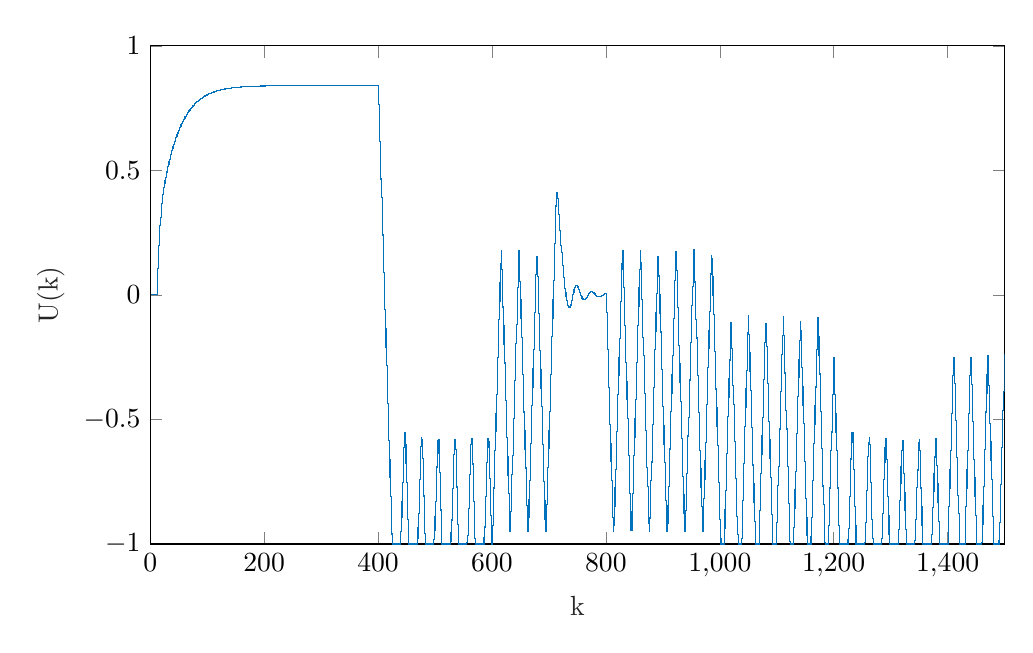
\begin{tikzpicture}

\begin{axis}[%
width=4.272in,
height=2.491in,
at={(0.717in,0.423in)},
scale only axis,
xmin=0,
xmax=1500,
xlabel style={font=\color{white!15!black}},
xlabel={k},
ymin=-1,
ymax=1,
ylabel style={font=\color{white!15!black}},
ylabel={U(k)},
axis background/.style={fill=white}
]
\addplot[const plot, color=mycolor1, forget plot] table[row sep=crcr] {%
1	0\\
2	0\\
3	0\\
4	0\\
5	0\\
6	0\\
7	0\\
8	0\\
9	0\\
10	0\\
11	0\\
12	0.0536431886114441\\
13	0.104247419384305\\
14	0.151910049514853\\
15	0.196765489796707\\
16	0.238961651573938\\
17	0.277901061638888\\
18	0.312196670498622\\
19	0.341165243395973\\
20	0.365187638439629\\
21	0.385285326382947\\
22	0.402590578706981\\
23	0.418023435285732\\
24	0.432207858880227\\
25	0.445521921675697\\
26	0.458181595904405\\
27	0.4703093438269\\
28	0.481976488001972\\
29	0.493228080492764\\
30	0.504094835739553\\
31	0.514599387536286\\
32	0.524759707138678\\
33	0.534591005817862\\
34	0.5441067918706\\
35	0.553319414887299\\
36	0.562240329497622\\
37	0.570880230739706\\
38	0.579249142234296\\
39	0.587356490496926\\
40	0.595211173469954\\
41	0.60282162246323\\
42	0.610195855826442\\
43	0.617341524042366\\
44	0.62426594708403\\
45	0.630976145281407\\
46	0.637478864951695\\
47	0.643780599838521\\
48	0.649887609190597\\
49	0.655805933136111\\
50	0.661541405874003\\
51	0.667099667098471\\
52	0.672486171989299\\
53	0.677706200033152\\
54	0.682764862887091\\
55	0.687667111453056\\
56	0.692417742298557\\
57	0.697021403532457\\
58	0.701482600223761\\
59	0.705805699434612\\
60	0.709994934925194\\
61	0.71405441157748\\
62	0.71798810957595\\
63	0.721799888376424\\
64	0.72549349048842\\
65	0.729072545091879\\
66	0.7325405715054\\
67	0.735900982520093\\
68	0.739157087610795\\
69	0.742312096034376\\
70	0.745369119823319\\
71	0.748331176681457\\
72	0.751201192787726\\
73	0.753982005512926\\
74	0.756676366053829\\
75	0.759286941988406\\
76	0.761816319755498\\
77	0.764267007061882\\
78	0.7666414352194\\
79	0.768941961414568\\
80	0.771170870912872\\
81	0.773330379199818\\
82	0.775422634060628\\
83	0.77744971760041\\
84	0.779413648206489\\
85	0.781316382454523\\
86	0.783159816959972\\
87	0.784945790176404\\
88	0.786676084142081\\
89	0.788352426176222\\
90	0.789976490526304\\
91	0.791549899967691\\
92	0.793074227356905\\
93	0.794550997139753\\
94	0.79598168681555\\
95	0.797367728358599\\
96	0.798710509598113\\
97	0.800011375557681\\
98	0.8012716297554\\
99	0.802492535465747\\
100	0.803675316944228\\
101	0.804821160615853\\
102	0.805931216228429\\
103	0.80700659797164\\
104	0.808048385562893\\
105	0.809057625300839\\
106	0.810035331087495\\
107	0.810982485419842\\
108	0.811900040351773\\
109	0.812788918427234\\
110	0.813650013585376\\
111	0.814484192038517\\
112	0.815292293123708\\
113	0.816075130128649\\
114	0.816833491092702\\
115	0.817568139583729\\
116	0.818279815451443\\
117	0.818969235557966\\
118	0.819637094486262\\
119	0.820284065227084\\
120	0.820910799845069\\
121	0.821517930124591\\
122	0.822106068195984\\
123	0.822675807142684\\
124	0.823227721589882\\
125	0.82376236827523\\
126	0.824280286602116\\
127	0.824781999176048\\
128	0.825268012324641\\
129	0.825738816601689\\
130	0.826194887275812\\
131	0.826636684804127\\
132	0.8270646552914\\
133	0.827479230935112\\
134	0.827880830456857\\
135	0.828269859520494\\
136	0.828646711137443\\
137	0.829011766059518\\
138	0.829365393159666\\
139	0.829707949800994\\
140	0.830039782194415\\
141	0.830361225745279\\
142	0.830672605389311\\
143	0.830974235918185\\
144	0.831266422295048\\
145	0.831549459960302\\
146	0.831823635127934\\
147	0.832089225072689\\
148	0.832346498408367\\
149	0.832595715357505\\
150	0.832837128012711\\
151	0.833070980589921\\
152	0.833297509673792\\
153	0.833516944455513\\
154	0.833729506963229\\
155	0.833935412285331\\
156	0.834134868786818\\
157	0.834328078318946\\
158	0.834515236422372\\
159	0.834696532523992\\
160	0.834872150127666\\
161	0.835042266999021\\
162	0.83520705534451\\
163	0.835366681984907\\
164	0.835521308523412\\
165	0.835671091508525\\
166	0.835816182591855\\
167	0.835956728681024\\
168	0.836092872087811\\
169	0.836224750671681\\
170	0.836352497978857\\
171	0.836476243377049\\
172	0.836596112186\\
173	0.836712225803956\\
174	0.8368247018302\\
175	0.836933654183773\\
176	0.837039193218483\\
177	0.837141425834343\\
178	0.837240455585525\\
179	0.837336382784951\\
180	0.837429304605627\\
181	0.837519315178807\\
182	0.837606505689103\\
183	0.837690964466627\\
184	0.837772777076252\\
185	0.837852026404092\\
186	0.837928792741286\\
187	0.838003153865156\\
188	0.838075185117847\\
189	0.838144959482493\\
190	0.838212547657023\\
191	0.838278018125649\\
192	0.838341437228127\\
193	0.838402869226852\\
194	0.838462376371861\\
195	0.8385200189638\\
196	0.838575855414927\\
197	0.838629942308208\\
198	0.838682334454565\\
199	0.838733084948336\\
200	0.838782245221001\\
201	0.838829865093232\\
202	0.838875992825307\\
203	0.838920675165956\\
204	0.83896395739968\\
205	0.839005883392583\\
206	0.839046495636778\\
207	0.839085835293401\\
208	0.839123942234282\\
209	0.839160855082308\\
210	0.839196611250529\\
211	0.839231246980039\\
212	0.839264797376669\\
213	0.839297296446534\\
214	0.839328777130471\\
215	0.839359271337397\\
216	0.839388809976619\\
217	0.83941742298914\\
218	0.839445139377984\\
219	0.839471987237565\\
220	0.839497993782149\\
221	0.839523185373413\\
222	0.839547587547149\\
223	0.839571225039132\\
224	0.839594121810173\\
225	0.839616301070396\\
226	0.839637785302744\\
227	0.839658596285761\\
228	0.839678755115654\\
229	0.839698282227663\\
230	0.83971719741677\\
231	0.839735519857747\\
232	0.839753268124591\\
233	0.839770460209338\\
234	0.839787113540296\\
235	0.8398032449997\\
236	0.839818870940825\\
237	0.839834007204549\\
238	0.839848669135411\\
239	0.839862871597156\\
240	0.839876628987798\\
241	0.83988995525421\\
242	0.83990286390626\\
243	0.839915368030499\\
244	0.839927480303423\\
245	0.839939213004321\\
246	0.83995057802772\\
247	0.839961586895436\\
248	0.839972250768256\\
249	0.839982580457246\\
250	0.839992586434707\\
251	0.840002278844793\\
252	0.840011667513787\\
253	0.840020761960066\\
254	0.840029571403742\\
255	0.840038104776013\\
256	0.840046370728211\\
257	0.840054377640575\\
258	0.840062133630739\\
259	0.840069646561966\\
260	0.840076924051116\\
261	0.840083973476365\\
262	0.840090801984688\\
263	0.840097416499096\\
264	0.840103823725664\\
265	0.840110030160316\\
266	0.840116042095423\\
267	0.840121865626169\\
268	0.840127506656739\\
269	0.840132970906299\\
270	0.840138263914795\\
271	0.840143391048566\\
272	0.840148357505791\\
273	0.840153168321749\\
274	0.840157828373931\\
275	0.840162342386982\\
276	0.840166714937487\\
277	0.840170950458615\\
278	0.840175053244613\\
279	0.840179027455157\\
280	0.840182877119567\\
281	0.840186606140898\\
282	0.840190218299891\\
283	0.840193717258808\\
284	0.840197106565147\\
285	0.840200389655231\\
286	0.840203569857702\\
287	0.840206650396887\\
288	0.840209634396069\\
289	0.840212524880658\\
290	0.84021532478125\\
291	0.840218036936605\\
292	0.840220664096521\\
293	0.840223208924625\\
294	0.840225674001069\\
295	0.840228061825149\\
296	0.840230374817838\\
297	0.840232615324242\\
298	0.840234785615974\\
299	0.840236887893458\\
300	0.840238924288164\\
301	0.840240896864764\\
302	0.840242807623226\\
303	0.840244658500844\\
304	0.840246451374199\\
305	0.840248188061066\\
306	0.840249870322252\\
307	0.840251499863383\\
308	0.840253078336635\\
309	0.840254607342406\\
310	0.840256088430941\\
311	0.840257523103904\\
312	0.840258912815897\\
313	0.840260258975938\\
314	0.840261562948889\\
315	0.840262826056839\\
316	0.840264049580446\\
317	0.840265234760231\\
318	0.840266382797841\\
319	0.840267494857267\\
320	0.840268572066018\\
321	0.840269615516273\\
322	0.840270626265979\\
323	0.840271605339933\\
324	0.840272553730813\\
325	0.84027347240019\\
326	0.8402743622795\\
327	0.840275224270988\\
328	0.840276059248625\\
329	0.840276868058993\\
330	0.840277651522144\\
331	0.840278410432428\\
332	0.840279145559303\\
333	0.840279857648115\\
334	0.840280547420847\\
335	0.840281215576862\\
336	0.8402818627936\\
337	0.840282489727275\\
338	0.840283097013534\\
339	0.840283685268106\\
340	0.84028425508742\\
341	0.840284807049217\\
342	0.840285341713132\\
343	0.84028585962126\\
344	0.840286361298708\\
345	0.840286847254128\\
346	0.840287317980229\\
347	0.840287773954283\\
348	0.840288215638602\\
349	0.840288643481009\\
350	0.840289057915295\\
351	0.840289459361655\\
352	0.840289848227117\\
353	0.840290224905952\\
354	0.840290589780075\\
355	0.840290943219434\\
356	0.84029128558238\\
357	0.840291617216036\\
358	0.840291938456647\\
359	0.84029224962992\\
360	0.840292551051353\\
361	0.840292843026559\\
362	0.840293125851571\\
363	0.840293399813148\\
364	0.84029366518906\\
365	0.840293922248372\\
366	0.840294171251716\\
367	0.84029441245156\\
368	0.840294646092455\\
369	0.840294872411291\\
370	0.840295091637534\\
371	0.840295303993458\\
372	0.840295509694371\\
373	0.840295708948834\\
374	0.840295901958872\\
375	0.840296088920179\\
376	0.840296270022314\\
377	0.8402964454489\\
378	0.8402966153778\\
379	0.840296779981307\\
380	0.840296939426313\\
381	0.84029709387448\\
382	0.840297243482403\\
383	0.84029738840177\\
384	0.840297528779517\\
385	0.840297664757972\\
386	0.840297796475004\\
387	0.840297924064163\\
388	0.840298047654811\\
389	0.840298167372257\\
390	0.840298283337883\\
391	0.840298395669268\\
392	0.840298504480305\\
393	0.840298609881317\\
394	0.840298711979172\\
395	0.840298810877386\\
396	0.840298906676234\\
397	0.840298999472845\\
398	0.840299089361308\\
399	0.84029917643276\\
400	0.840299260775483\\
401	0.765299260775483\\
402	0.690299260775483\\
403	0.615299260775483\\
404	0.540299260775483\\
405	0.465299260775483\\
406	0.390299260775483\\
407	0.315299260775483\\
408	0.240299260775483\\
409	0.165299260775483\\
410	0.0902992607754834\\
411	0.0152992607754834\\
412	-0.0597007392245166\\
413	-0.134700739224517\\
414	-0.209700739224517\\
415	-0.284700739224517\\
416	-0.359700739224517\\
417	-0.434700739224517\\
418	-0.509700739224517\\
419	-0.584700739224517\\
420	-0.659700739224517\\
421	-0.734700739224517\\
422	-0.809700739224516\\
423	-0.884700739224516\\
424	-0.959700739224516\\
425	-1\\
426	-1\\
427	-1\\
428	-1\\
429	-1\\
430	-1\\
431	-1\\
432	-1\\
433	-1\\
434	-1\\
435	-1\\
436	-1\\
437	-1\\
438	-1\\
439	-0.988549684813738\\
440	-0.950412712289044\\
441	-0.894409065454579\\
442	-0.827600708094603\\
443	-0.75469167489761\\
444	-0.679832683492975\\
445	-0.610889556103326\\
446	-0.561569135576498\\
447	-0.551084284180199\\
448	-0.602490824790468\\
449	-0.677490824790468\\
450	-0.752490824790468\\
451	-0.827490824790468\\
452	-0.902490824790468\\
453	-0.977490824790468\\
454	-1\\
455	-1\\
456	-1\\
457	-1\\
458	-1\\
459	-1\\
460	-1\\
461	-1\\
462	-1\\
463	-1\\
464	-1\\
465	-1\\
466	-1\\
467	-1\\
468	-1\\
469	-0.976485489358023\\
470	-0.932882955064664\\
471	-0.876070957084135\\
472	-0.811063218022137\\
473	-0.740993782375297\\
474	-0.670770842674428\\
475	-0.610095279006221\\
476	-0.574088335617945\\
477	-0.582325984430809\\
478	-0.65712037924943\\
479	-0.73212037924943\\
480	-0.80712037924943\\
481	-0.88212037924943\\
482	-0.95712037924943\\
483	-1\\
484	-1\\
485	-1\\
486	-1\\
487	-1\\
488	-1\\
489	-1\\
490	-1\\
491	-1\\
492	-1\\
493	-1\\
494	-1\\
495	-1\\
496	-1\\
497	-1\\
498	-0.983140577411292\\
499	-0.944570180597197\\
500	-0.891352153940876\\
501	-0.828873744428978\\
502	-0.760631554575027\\
503	-0.690886196027753\\
504	-0.627976273799917\\
505	-0.58553168643642\\
506	-0.581864564257429\\
507	-0.638435135477908\\
508	-0.713435135477908\\
509	-0.788435135477908\\
510	-0.863435135477908\\
511	-0.938435135477908\\
512	-1\\
513	-1\\
514	-1\\
515	-1\\
516	-1\\
517	-1\\
518	-1\\
519	-1\\
520	-1\\
521	-1\\
522	-1\\
523	-1\\
524	-1\\
525	-1\\
526	-1\\
527	-0.988850221501658\\
528	-0.954337298538669\\
529	-0.903796987003297\\
530	-0.843035725831477\\
531	-0.775926110841609\\
532	-0.706208204207058\\
533	-0.641110457151552\\
534	-0.593091062528884\\
535	-0.579526938938439\\
536	-0.621312578501298\\
537	-0.696312578501297\\
538	-0.771312578501297\\
539	-0.846312578501297\\
540	-0.921312578501297\\
541	-0.996312578501297\\
542	-1\\
543	-1\\
544	-1\\
545	-1\\
546	-1\\
547	-1\\
548	-1\\
549	-1\\
550	-1\\
551	-1\\
552	-1\\
553	-1\\
554	-1\\
555	-1\\
556	-0.994694473716242\\
557	-0.964292108390109\\
558	-0.916426156255436\\
559	-0.857348311226044\\
560	-0.791326669418261\\
561	-0.721579150976082\\
562	-0.654217887038837\\
563	-0.600530385256809\\
564	-0.576967627555213\\
565	-0.60387206238011\\
566	-0.67887206238011\\
567	-0.75387206238011\\
568	-0.82887206238011\\
569	-0.90387206238011\\
570	-0.97887206238011\\
571	-1\\
572	-1\\
573	-1\\
574	-1\\
575	-1\\
576	-1\\
577	-1\\
578	-1\\
579	-1\\
580	-1\\
581	-1\\
582	-1\\
583	-1\\
584	-1\\
585	-1\\
586	-0.975545628893779\\
587	-0.931751819669803\\
588	-0.875243357662805\\
589	-0.810783818813726\\
590	-0.74132620698737\\
591	-0.671813601760112\\
592	-0.612051359681462\\
593	-0.57718808806316\\
594	-0.586702203890346\\
595	-0.661702203890346\\
596	-0.736702203890346\\
597	-0.811702203890346\\
598	-0.886702203890346\\
599	-0.961702203890346\\
600	-1\\
601	-0.925\\
602	-0.85\\
603	-0.775\\
604	-0.7\\
605	-0.625\\
606	-0.55\\
607	-0.475\\
608	-0.4\\
609	-0.325\\
610	-0.25\\
611	-0.175\\
612	-0.1\\
613	-0.0250000000000002\\
614	0.0499999999999998\\
615	0.125\\
616	0.176461132995605\\
617	0.101461132995605\\
618	0.0264611329956047\\
619	-0.0485388670043953\\
620	-0.123538867004395\\
621	-0.198538867004395\\
622	-0.273538867004395\\
623	-0.348538867004395\\
624	-0.423538867004395\\
625	-0.498538867004395\\
626	-0.573538867004395\\
627	-0.648538867004395\\
628	-0.723538867004395\\
629	-0.798538867004395\\
630	-0.873538867004395\\
631	-0.947687671771061\\
632	-0.945182955951875\\
633	-0.870182955951875\\
634	-0.795182955951875\\
635	-0.720182955951875\\
636	-0.645182955951875\\
637	-0.570182955951875\\
638	-0.495182955951875\\
639	-0.420182955951875\\
640	-0.345182955951875\\
641	-0.270182955951875\\
642	-0.195182955951875\\
643	-0.120182955951875\\
644	-0.045182955951875\\
645	0.029817044048125\\
646	0.104817044048125\\
647	0.179817044048125\\
648	0.130020908299168\\
649	0.0550209082991679\\
650	-0.0199790917008321\\
651	-0.0949790917008321\\
652	-0.169979091700832\\
653	-0.244979091700832\\
654	-0.319979091700832\\
655	-0.394979091700832\\
656	-0.469979091700832\\
657	-0.544979091700832\\
658	-0.619979091700832\\
659	-0.694979091700832\\
660	-0.769979091700832\\
661	-0.844979091700832\\
662	-0.919979091700832\\
663	-0.947889732215666\\
664	-0.894813507046258\\
665	-0.819813507046258\\
666	-0.744813507046258\\
667	-0.669813507046258\\
668	-0.594813507046258\\
669	-0.519813507046258\\
670	-0.444813507046258\\
671	-0.369813507046258\\
672	-0.294813507046258\\
673	-0.219813507046258\\
674	-0.144813507046258\\
675	-0.0698135070462583\\
676	0.00518649295374166\\
677	0.0801864929537417\\
678	0.155186492953742\\
679	0.150287948989609\\
680	0.0752879489896092\\
681	0.000287948989609182\\
682	-0.0747120510103908\\
683	-0.149712051010391\\
684	-0.224712051010391\\
685	-0.299712051010391\\
686	-0.374712051010391\\
687	-0.449712051010391\\
688	-0.524712051010391\\
689	-0.599712051010391\\
690	-0.674712051010391\\
691	-0.749712051010391\\
692	-0.824712051010391\\
693	-0.899712051010391\\
694	-0.948353475166179\\
695	-0.917870157822396\\
696	-0.842870157822396\\
697	-0.767870157822396\\
698	-0.692870157822396\\
699	-0.617870157822397\\
700	-0.542870157822397\\
701	-0.467870157822397\\
702	-0.392870157822397\\
703	-0.317870157822397\\
704	-0.242870157822397\\
705	-0.167870157822397\\
706	-0.0928701578223965\\
707	-0.0178701578223965\\
708	0.0571298421776035\\
709	0.132129842177603\\
710	0.207129842177603\\
711	0.282129842177604\\
712	0.357129842177604\\
713	0.407152298195652\\
714	0.409181127120838\\
715	0.387215900028918\\
716	0.355755549520326\\
717	0.322256761380937\\
718	0.289670447317697\\
719	0.258450869513545\\
720	0.228391509822784\\
721	0.199300073062661\\
722	0.171133004167529\\
723	0.143955012548601\\
724	0.117873497407346\\
725	0.0930073045682854\\
726	0.0694856936903674\\
727	0.0474582607105296\\
728	0.0271025875116345\\
729	0.00862512944262362\\
730	-0.00774491660458453\\
731	-0.0217675383468543\\
732	-0.0332072419296553\\
733	-0.0418518049817776\\
734	-0.047534476690686\\
735	-0.0501590123655818\\
736	-0.0497258578042644\\
737	-0.0463566003347788\\
738	-0.0403128181077806\\
739	-0.0320048725009966\\
740	-0.0219862349599605\\
741	-0.0109299259874671\\
742	0.00041414286723516\\
743	0.0112786318327856\\
744	0.0209483997629152\\
745	0.0288295998005219\\
746	0.034505493811498\\
747	0.0377677584162155\\
748	0.038617516721544\\
749	0.0372381234729686\\
750	0.0339487550347116\\
751	0.0291512256454733\\
752	0.0232812412664337\\
753	0.0167708968518158\\
754	0.0100241297349172\\
755	0.00340310288711067\\
756	-0.00277814002082635\\
757	-0.00825629406211842\\
758	-0.0128202062032824\\
759	-0.0163123911835955\\
760	-0.0186309685126093\\
761	-0.019731675346546\\
762	-0.0196292278266994\\
763	-0.0183971294564272\\
764	-0.0161650186664294\\
765	-0.0131128044208125\\
766	-0.00946116513866549\\
767	-0.00545847055104314\\
768	-0.00136477730696801\\
769	0.00256585010029513\\
770	0.00610296418124831\\
771	0.00905536083580386\\
772	0.0112829080166465\\
773	0.0127032939151544\\
774	0.0132932000863686\\
775	0.0130842730328246\\
776	0.0121549951857947\\
777	0.0106199742702018\\
778	0.0086182206406007\\
779	0.00630172581001426\\
780	0.00382522939684486\\
781	0.00133761644317598\\
782	-0.00102496671485877\\
783	-0.00314440313386677\\
784	-0.00492450616370165\\
785	-0.00629371595588001\\
786	-0.00720670888188691\\
787	-0.0076449600124222\\
788	-0.00761624103149236\\
789	-0.00715301360998102\\
790	-0.00630969727720261\\
791	-0.00515884912072273\\
792	-0.00378638134749247\\
793	-0.00228604709423839\\
794	-0.000753525685619476\\
795	0.000719485141931916\\
796	0.00205072944301828\\
797	0.00317198724116463\\
798	0.00403246317869589\\
799	0.00460075545328758\\
800	0.00486534188111195\\
801	-0.070134658118888\\
802	-0.145134658118888\\
803	-0.220134658118888\\
804	-0.295134658118888\\
805	-0.370134658118888\\
806	-0.445134658118888\\
807	-0.520134658118888\\
808	-0.595134658118888\\
809	-0.670134658118888\\
810	-0.745134658118888\\
811	-0.820134658118888\\
812	-0.895134658118888\\
813	-0.949247661187076\\
814	-0.924930797615347\\
815	-0.849930797615347\\
816	-0.774930797615347\\
817	-0.699930797615347\\
818	-0.624930797615347\\
819	-0.549930797615347\\
820	-0.474930797615347\\
821	-0.399930797615347\\
822	-0.324930797615347\\
823	-0.249930797615347\\
824	-0.174930797615347\\
825	-0.0999307976153474\\
826	-0.0249307976153474\\
827	0.0500692023846526\\
828	0.125069202384653\\
829	0.178941043113911\\
830	0.103941043113911\\
831	0.0289410431139115\\
832	-0.0460589568860885\\
833	-0.121058956886089\\
834	-0.196058956886089\\
835	-0.271058956886089\\
836	-0.346058956886089\\
837	-0.421058956886089\\
838	-0.496058956886089\\
839	-0.571058956886089\\
840	-0.646058956886088\\
841	-0.721058956886088\\
842	-0.796058956886088\\
843	-0.871058956886088\\
844	-0.946058956886088\\
845	-0.946209591373924\\
846	-0.871209591373924\\
847	-0.796209591373924\\
848	-0.721209591373924\\
849	-0.646209591373924\\
850	-0.571209591373924\\
851	-0.496209591373924\\
852	-0.421209591373924\\
853	-0.346209591373924\\
854	-0.271209591373924\\
855	-0.196209591373924\\
856	-0.121209591373924\\
857	-0.0462095913739243\\
858	0.0287904086260757\\
859	0.103790408626076\\
860	0.178790408626076\\
861	0.130798574653694\\
862	0.0557985746536938\\
863	-0.0192014253463062\\
864	-0.0942014253463062\\
865	-0.169201425346306\\
866	-0.244201425346306\\
867	-0.319201425346306\\
868	-0.394201425346306\\
869	-0.469201425346306\\
870	-0.544201425346306\\
871	-0.619201425346306\\
872	-0.694201425346306\\
873	-0.769201425346306\\
874	-0.844201425346306\\
875	-0.919201425346306\\
876	-0.947923870503041\\
877	-0.895729894488563\\
878	-0.820729894488563\\
879	-0.745729894488563\\
880	-0.670729894488563\\
881	-0.595729894488563\\
882	-0.520729894488563\\
883	-0.445729894488563\\
884	-0.370729894488563\\
885	-0.295729894488563\\
886	-0.220729894488563\\
887	-0.145729894488563\\
888	-0.0707298944885629\\
889	0.00427010551143706\\
890	0.0792701055114371\\
891	0.154270105511437\\
892	0.15110283993824\\
893	0.0761028399382402\\
894	0.00110283993824023\\
895	-0.0738971600617598\\
896	-0.14889716006176\\
897	-0.22389716006176\\
898	-0.29889716006176\\
899	-0.37389716006176\\
900	-0.44889716006176\\
901	-0.52389716006176\\
902	-0.59889716006176\\
903	-0.67389716006176\\
904	-0.74889716006176\\
905	-0.82389716006176\\
906	-0.89889716006176\\
907	-0.948353910492429\\
908	-0.918761829813893\\
909	-0.843761829813893\\
910	-0.768761829813894\\
911	-0.693761829813894\\
912	-0.618761829813894\\
913	-0.543761829813894\\
914	-0.468761829813894\\
915	-0.393761829813894\\
916	-0.318761829813894\\
917	-0.243761829813894\\
918	-0.168761829813894\\
919	-0.0937618298138936\\
920	-0.0187618298138936\\
921	0.0562381701861064\\
922	0.131238170186106\\
923	0.17269172887151\\
924	0.0976917288715097\\
925	0.0226917288715097\\
926	-0.0523082711284902\\
927	-0.12730827112849\\
928	-0.20230827112849\\
929	-0.27730827112849\\
930	-0.35230827112849\\
931	-0.42730827112849\\
932	-0.50230827112849\\
933	-0.57730827112849\\
934	-0.65230827112849\\
935	-0.72730827112849\\
936	-0.80230827112849\\
937	-0.87730827112849\\
938	-0.947862438382825\\
939	-0.941404881702848\\
940	-0.866404881702848\\
941	-0.791404881702848\\
942	-0.716404881702848\\
943	-0.641404881702848\\
944	-0.566404881702848\\
945	-0.491404881702848\\
946	-0.416404881702848\\
947	-0.341404881702848\\
948	-0.266404881702848\\
949	-0.191404881702848\\
950	-0.116404881702848\\
951	-0.0414048817028484\\
952	0.0335951182971516\\
953	0.108595118297152\\
954	0.183595118297152\\
955	0.126998446795546\\
956	0.0519984467955456\\
957	-0.0230015532044544\\
958	-0.0980015532044544\\
959	-0.173001553204454\\
960	-0.248001553204454\\
961	-0.323001553204454\\
962	-0.398001553204454\\
963	-0.473001553204454\\
964	-0.548001553204454\\
965	-0.623001553204454\\
966	-0.698001553204454\\
967	-0.773001553204454\\
968	-0.848001553204454\\
969	-0.923001553204454\\
970	-0.94774892555982\\
971	-0.891235077734798\\
972	-0.816235077734798\\
973	-0.741235077734798\\
974	-0.666235077734798\\
975	-0.591235077734798\\
976	-0.516235077734798\\
977	-0.441235077734798\\
978	-0.366235077734798\\
979	-0.291235077734798\\
980	-0.216235077734798\\
981	-0.141235077734798\\
982	-0.0662350777347982\\
983	0.00876492226520179\\
984	0.0837649222652018\\
985	0.158764922265202\\
986	0.147140175247815\\
987	0.0721401752478147\\
988	-0.00285982475218527\\
989	-0.0778598247521853\\
990	-0.152859824752185\\
991	-0.227859824752185\\
992	-0.302859824752185\\
993	-0.377859824752185\\
994	-0.452859824752185\\
995	-0.527859824752185\\
996	-0.602859824752185\\
997	-0.677859824752185\\
998	-0.752859824752185\\
999	-0.827859824752185\\
1000	-0.902859824752185\\
1001	-0.977859824752185\\
1002	-1\\
1003	-1\\
1004	-1\\
1005	-1\\
1006	-1\\
1007	-1\\
1008	-0.936475530856021\\
1009	-0.861475530856021\\
1010	-0.786475530856021\\
1011	-0.711475530856021\\
1012	-0.636475530856021\\
1013	-0.561475530856022\\
1014	-0.486475530856022\\
1015	-0.411475530856022\\
1016	-0.336475530856021\\
1017	-0.261475530856021\\
1018	-0.186475530856021\\
1019	-0.111475530856021\\
1020	-0.138512916735401\\
1021	-0.213512916735401\\
1022	-0.288512916735401\\
1023	-0.363512916735401\\
1024	-0.438512916735401\\
1025	-0.513512916735401\\
1026	-0.588512916735401\\
1027	-0.663512916735401\\
1028	-0.738512916735401\\
1029	-0.813512916735401\\
1030	-0.888512916735401\\
1031	-0.963512916735401\\
1032	-1\\
1033	-1\\
1034	-1\\
1035	-1\\
1036	-1\\
1037	-1\\
1038	-0.976720524568846\\
1039	-0.901720524568846\\
1040	-0.826720524568846\\
1041	-0.751720524568846\\
1042	-0.676720524568846\\
1043	-0.601720524568847\\
1044	-0.526720524568847\\
1045	-0.451720524568847\\
1046	-0.376720524568847\\
1047	-0.301720524568847\\
1048	-0.226720524568847\\
1049	-0.151720524568846\\
1050	-0.0829398785298861\\
1051	-0.157939878529886\\
1052	-0.232939878529886\\
1053	-0.307939878529886\\
1054	-0.382939878529886\\
1055	-0.457939878529886\\
1056	-0.532939878529886\\
1057	-0.607939878529886\\
1058	-0.682939878529886\\
1059	-0.757939878529886\\
1060	-0.832939878529886\\
1061	-0.907939878529886\\
1062	-0.982939878529886\\
1063	-1\\
1064	-1\\
1065	-1\\
1066	-1\\
1067	-1\\
1068	-1\\
1069	-0.940819982418964\\
1070	-0.865819982418964\\
1071	-0.790819982418964\\
1072	-0.715819982418964\\
1073	-0.640819982418964\\
1074	-0.565819982418964\\
1075	-0.490819982418964\\
1076	-0.415819982418964\\
1077	-0.340819982418964\\
1078	-0.265819982418964\\
1079	-0.190819982418964\\
1080	-0.115819982418964\\
1081	-0.131701752363398\\
1082	-0.206701752363398\\
1083	-0.281701752363398\\
1084	-0.356701752363398\\
1085	-0.431701752363398\\
1086	-0.506701752363398\\
1087	-0.581701752363398\\
1088	-0.656701752363398\\
1089	-0.731701752363398\\
1090	-0.806701752363398\\
1091	-0.881701752363398\\
1092	-0.956701752363398\\
1093	-1\\
1094	-1\\
1095	-1\\
1096	-1\\
1097	-1\\
1098	-1\\
1099	-0.988475847970267\\
1100	-0.913475847970267\\
1101	-0.838475847970268\\
1102	-0.763475847970268\\
1103	-0.688475847970268\\
1104	-0.613475847970268\\
1105	-0.538475847970268\\
1106	-0.463475847970268\\
1107	-0.388475847970268\\
1108	-0.313475847970268\\
1109	-0.238475847970268\\
1110	-0.163475847970268\\
1111	-0.0884758479702677\\
1112	-0.163475847970268\\
1113	-0.238475847970268\\
1114	-0.313475847970268\\
1115	-0.388475847970268\\
1116	-0.463475847970268\\
1117	-0.538475847970268\\
1118	-0.613475847970268\\
1119	-0.688475847970268\\
1120	-0.763475847970268\\
1121	-0.838475847970268\\
1122	-0.913475847970267\\
1123	-0.988475847970267\\
1124	-1\\
1125	-1\\
1126	-1\\
1127	-1\\
1128	-1\\
1129	-1\\
1130	-0.932875003134913\\
1131	-0.857875003134913\\
1132	-0.782875003134913\\
1133	-0.707875003134913\\
1134	-0.632875003134913\\
1135	-0.557875003134913\\
1136	-0.482875003134913\\
1137	-0.407875003134913\\
1138	-0.332875003134913\\
1139	-0.257875003134913\\
1140	-0.182875003134913\\
1141	-0.107875003134913\\
1142	-0.142454208488569\\
1143	-0.217454208488569\\
1144	-0.292454208488569\\
1145	-0.367454208488569\\
1146	-0.442454208488569\\
1147	-0.517454208488569\\
1148	-0.592454208488569\\
1149	-0.667454208488569\\
1150	-0.742454208488569\\
1151	-0.817454208488569\\
1152	-0.892454208488568\\
1153	-0.967454208488568\\
1154	-1\\
1155	-1\\
1156	-1\\
1157	-1\\
1158	-1\\
1159	-1\\
1160	-0.969784326455708\\
1161	-0.894784326455708\\
1162	-0.819784326455708\\
1163	-0.744784326455708\\
1164	-0.669784326455708\\
1165	-0.594784326455708\\
1166	-0.519784326455708\\
1167	-0.444784326455708\\
1168	-0.369784326455708\\
1169	-0.294784326455708\\
1170	-0.219784326455708\\
1171	-0.144784326455708\\
1172	-0.0923087182349367\\
1173	-0.167308718234937\\
1174	-0.242308718234937\\
1175	-0.317308718234937\\
1176	-0.392308718234937\\
1177	-0.467308718234937\\
1178	-0.542308718234937\\
1179	-0.617308718234937\\
1180	-0.692308718234937\\
1181	-0.767308718234937\\
1182	-0.842308718234937\\
1183	-0.917308718234937\\
1184	-0.992308718234936\\
1185	-1\\
1186	-1\\
1187	-1\\
1188	-1\\
1189	-1\\
1190	-1\\
1191	-0.925193637335256\\
1192	-0.850193637335256\\
1193	-0.775193637335256\\
1194	-0.700193637335256\\
1195	-0.625193637335256\\
1196	-0.550193637335256\\
1197	-0.475193637335256\\
1198	-0.400193637335256\\
1199	-0.325193637335256\\
1200	-0.250193637335256\\
1201	-0.325193637335256\\
1202	-0.400193637335256\\
1203	-0.475193637335256\\
1204	-0.550193637335256\\
1205	-0.625193637335256\\
1206	-0.700193637335256\\
1207	-0.775193637335256\\
1208	-0.850193637335256\\
1209	-0.925193637335256\\
1210	-1\\
1211	-1\\
1212	-1\\
1213	-1\\
1214	-1\\
1215	-1\\
1216	-1\\
1217	-1\\
1218	-1\\
1219	-1\\
1220	-1\\
1221	-1\\
1222	-1\\
1223	-1\\
1224	-1\\
1225	-0.98078463675157\\
1226	-0.937061183020972\\
1227	-0.877305570185924\\
1228	-0.808054233884119\\
1229	-0.733518291311555\\
1230	-0.658556798676149\\
1231	-0.592564195063476\\
1232	-0.550890184560421\\
1233	-0.554091070274986\\
1234	-0.626066093258415\\
1235	-0.701066093258415\\
1236	-0.776066093258414\\
1237	-0.851066093258414\\
1238	-0.926066093258414\\
1239	-1\\
1240	-1\\
1241	-1\\
1242	-1\\
1243	-1\\
1244	-1\\
1245	-1\\
1246	-1\\
1247	-1\\
1248	-1\\
1249	-1\\
1250	-1\\
1251	-1\\
1252	-1\\
1253	-1\\
1254	-0.994115471311677\\
1255	-0.962734160460807\\
1256	-0.913710459079609\\
1257	-0.853469228659726\\
1258	-0.786382299727145\\
1259	-0.715781189785778\\
1260	-0.647982469624312\\
1261	-0.594583758489237\\
1262	-0.572420145011379\\
1263	-0.602237092378636\\
1264	-0.677237092378635\\
1265	-0.752237092378635\\
1266	-0.827237092378635\\
1267	-0.902237092378635\\
1268	-0.977237092378635\\
1269	-1\\
1270	-1\\
1271	-1\\
1272	-1\\
1273	-1\\
1274	-1\\
1275	-1\\
1276	-1\\
1277	-1\\
1278	-1\\
1279	-1\\
1280	-1\\
1281	-1\\
1282	-1\\
1283	-1\\
1284	-0.976192968085138\\
1285	-0.932767789162113\\
1286	-0.876420196215872\\
1287	-0.811996025712332\\
1288	-0.742513756864399\\
1289	-0.672866332522675\\
1290	-0.612746396943299\\
1291	-0.577199429303338\\
1292	-0.585644685441622\\
1293	-0.660180464419965\\
1294	-0.735180464419965\\
1295	-0.810180464419965\\
1296	-0.885180464419965\\
1297	-0.960180464419965\\
1298	-1\\
1299	-1\\
1300	-1\\
1301	-1\\
1302	-1\\
1303	-1\\
1304	-1\\
1305	-1\\
1306	-1\\
1307	-1\\
1308	-1\\
1309	-1\\
1310	-1\\
1311	-1\\
1312	-1\\
1313	-0.982016841672431\\
1314	-0.942720122740994\\
1315	-0.889087904298627\\
1316	-0.826397473821494\\
1317	-0.758053373292012\\
1318	-0.688411436837585\\
1319	-0.626018008999314\\
1320	-0.584709928226881\\
1321	-0.582946535950074\\
1322	-0.642254572329418\\
1323	-0.717254572329418\\
1324	-0.792254572329418\\
1325	-0.867254572329418\\
1326	-0.942254572329418\\
1327	-1\\
1328	-1\\
1329	-1\\
1330	-1\\
1331	-1\\
1332	-1\\
1333	-1\\
1334	-1\\
1335	-1\\
1336	-1\\
1337	-1\\
1338	-1\\
1339	-1\\
1340	-1\\
1341	-1\\
1342	-0.987617171986871\\
1343	-0.952250635791883\\
1344	-0.901167395206182\\
1345	-0.840074758229674\\
1346	-0.772758463070454\\
1347	-0.703068019478855\\
1348	-0.63846676301146\\
1349	-0.591656928376622\\
1350	-0.580204860456028\\
1351	-0.625113195483284\\
1352	-0.700113195483284\\
1353	-0.775113195483284\\
1354	-0.850113195483284\\
1355	-0.925113195483284\\
1356	-1\\
1357	-1\\
1358	-1\\
1359	-1\\
1360	-1\\
1361	-1\\
1362	-1\\
1363	-1\\
1364	-1\\
1365	-1\\
1366	-1\\
1367	-1\\
1368	-1\\
1369	-1\\
1370	-1\\
1371	-0.993064062160199\\
1372	-0.961511632999607\\
1373	-0.91289442245926\\
1374	-0.853341167741079\\
1375	-0.787010457720525\\
1376	-0.717265631195479\\
1377	-0.650529509930383\\
1378	-0.598415951265242\\
1379	-0.577635055808099\\
1380	-0.608685239630803\\
1381	-0.683685239630803\\
1382	-0.758685239630803\\
1383	-0.833685239630803\\
1384	-0.908685239630803\\
1385	-0.983685239630803\\
1386	-1\\
1387	-1\\
1388	-1\\
1389	-1\\
1390	-1\\
1391	-1\\
1392	-1\\
1393	-1\\
1394	-1\\
1395	-1\\
1396	-1\\
1397	-1\\
1398	-1\\
1399	-1\\
1400	-1\\
1401	-0.925\\
1402	-0.85\\
1403	-0.775\\
1404	-0.7\\
1405	-0.625\\
1406	-0.55\\
1407	-0.475\\
1408	-0.4\\
1409	-0.325\\
1410	-0.25\\
1411	-0.279208332507245\\
1412	-0.354208332507245\\
1413	-0.429208332507245\\
1414	-0.504208332507245\\
1415	-0.579208332507245\\
1416	-0.654208332507245\\
1417	-0.729208332507245\\
1418	-0.804208332507245\\
1419	-0.879208332507245\\
1420	-0.954208332507245\\
1421	-1\\
1422	-1\\
1423	-1\\
1424	-1\\
1425	-1\\
1426	-1\\
1427	-1\\
1428	-1\\
1429	-1\\
1430	-1\\
1431	-0.925\\
1432	-0.85\\
1433	-0.775\\
1434	-0.7\\
1435	-0.625\\
1436	-0.55\\
1437	-0.475\\
1438	-0.4\\
1439	-0.325\\
1440	-0.25\\
1441	-0.284717695552023\\
1442	-0.359717695552023\\
1443	-0.434717695552023\\
1444	-0.509717695552024\\
1445	-0.584717695552023\\
1446	-0.659717695552023\\
1447	-0.734717695552023\\
1448	-0.809717695552023\\
1449	-0.884717695552023\\
1450	-0.959717695552023\\
1451	-1\\
1452	-1\\
1453	-1\\
1454	-1\\
1455	-1\\
1456	-1\\
1457	-1\\
1458	-1\\
1459	-1\\
1460	-0.994991532427031\\
1461	-0.919991532427031\\
1462	-0.844991532427031\\
1463	-0.769991532427031\\
1464	-0.694991532427031\\
1465	-0.619991532427031\\
1466	-0.544991532427031\\
1467	-0.469991532427031\\
1468	-0.394991532427031\\
1469	-0.319991532427031\\
1470	-0.244991532427031\\
1471	-0.290336605484695\\
1472	-0.365336605484695\\
1473	-0.440336605484695\\
1474	-0.515336605484695\\
1475	-0.590336605484695\\
1476	-0.665336605484695\\
1477	-0.740336605484695\\
1478	-0.815336605484695\\
1479	-0.890336605484695\\
1480	-0.965336605484695\\
1481	-1\\
1482	-1\\
1483	-1\\
1484	-1\\
1485	-1\\
1486	-1\\
1487	-1\\
1488	-1\\
1489	-1\\
1490	-0.98762702780892\\
1491	-0.91262702780892\\
1492	-0.83762702780892\\
1493	-0.76262702780892\\
1494	-0.68762702780892\\
1495	-0.61262702780892\\
1496	-0.53762702780892\\
1497	-0.46262702780892\\
1498	-0.38762702780892\\
1499	-0.31262702780892\\
1500	-0.23762702780892\\
};
\end{axis}
\end{tikzpicture}%
\caption{Regulacja DMC, $N = 15; N_u = 15; \lambda = 1$}
\end{figure}

\begin{figure}[H]
\centering
% This file was created by matlab2tikz.
%
%The latest updates can be retrieved from
%  http://www.mathworks.com/matlabcentral/fileexchange/22022-matlab2tikz-matlab2tikz
%where you can also make suggestions and rate matlab2tikz.
%
\definecolor{mycolor1}{rgb}{0.00000,0.44700,0.74100}%
\definecolor{mycolor2}{rgb}{0.85000,0.32500,0.09800}%
%
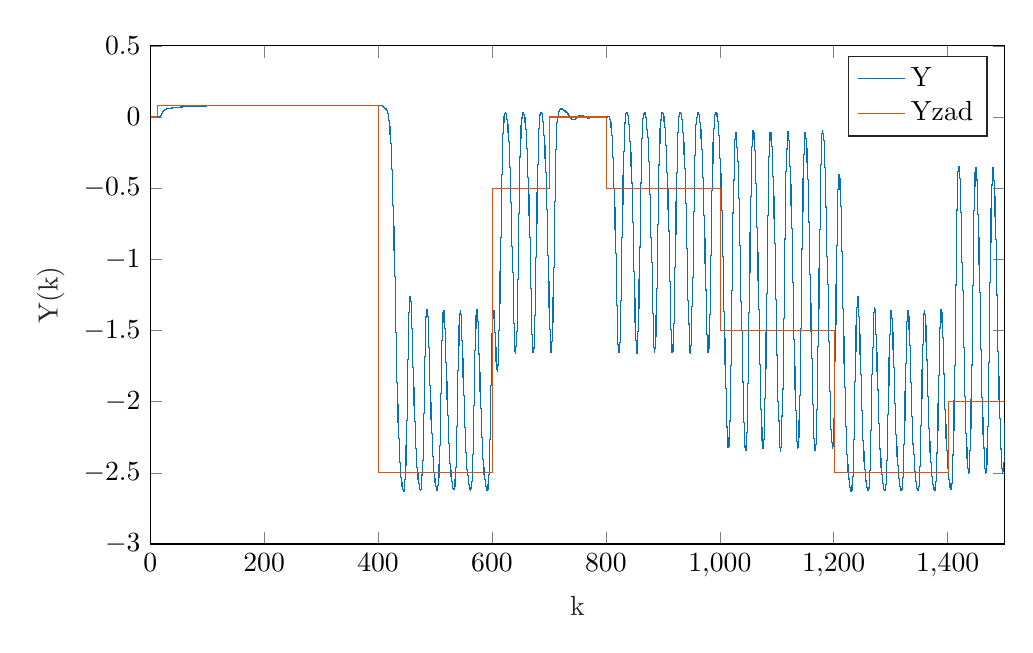
\begin{tikzpicture}

\begin{axis}[%
width=4.272in,
height=2.491in,
at={(0.717in,0.423in)},
scale only axis,
xmin=0,
xmax=1500,
xlabel style={font=\color{white!15!black}},
xlabel={k},
ymin=-3,
ymax=0.5,
ylabel style={font=\color{white!15!black}},
ylabel={Y(k)},
axis background/.style={fill=white},
legend style={legend cell align=left, align=left, draw=white!15!black}
]
\addplot[const plot, color=mycolor1] table[row sep=crcr] {%
1	0\\
2	0\\
3	0\\
4	0\\
5	0\\
6	0\\
7	0\\
8	0\\
9	0\\
10	0\\
11	0\\
12	0\\
13	0\\
14	0\\
15	0\\
16	0\\
17	0.00245004667951267\\
18	0.00873514143676791\\
19	0.0172103336589493\\
20	0.0258515554890762\\
21	0.0334115506406829\\
22	0.0394972548613088\\
23	0.0442153145536109\\
24	0.0478300772671608\\
25	0.0505989212245395\\
26	0.052732180824379\\
27	0.0543971866640866\\
28	0.0557264794956446\\
29	0.0568220210822203\\
30	0.0577582516051306\\
31	0.0585863967548774\\
32	0.0593398943942788\\
33	0.0600397528992867\\
34	0.060698915338902\\
35	0.0613253850863832\\
36	0.0619242398531089\\
37	0.0624988453975751\\
38	0.0630515597987373\\
39	0.0635841355082349\\
40	0.064097948552637\\
41	0.0645941297883215\\
42	0.0650736408447029\\
43	0.0655373191998054\\
44	0.0659859063366814\\
45	0.0664200666970329\\
46	0.0668404014803941\\
47	0.0672474593037042\\
48	0.0676417447108982\\
49	0.0680237250572567\\
50	0.0683938360985312\\
51	0.068752486530139\\
52	0.0691000616753935\\
53	0.0694369264869385\\
54	0.0697634279956987\\
55	0.0700798973160438\\
56	0.070386651294514\\
57	0.0706839938720751\\
58	0.0709722172158812\\
59	0.0712516026653152\\
60	0.0715224215281209\\
61	0.0717849357552975\\
62	0.0720393985177355\\
63	0.0722860547030431\\
64	0.0725251413473972\\
65	0.0727568880143622\\
66	0.0729815171303048\\
67	0.0731992442841759\\
68	0.0734102784979294\\
69	0.0736148224726486\\
70	0.0738130728144739\\
71	0.0740052202436462\\
72	0.0741914497893441\\
73	0.0743719409724848\\
74	0.0745468679782462\\
75	0.074716399819732\\
76	0.0748807004939381\\
77	0.0750399291309551\\
78	0.0751942401371734\\
79	0.0753437833331108\\
80	0.0754887040863721\\
81	0.0756291434401578\\
82	0.0757652382376639\\
83	0.075897121242658\\
84	0.0760249212564681\\
85	0.0761487632315805\\
86	0.0762687683820173\\
87	0.0763850542906344\\
88	0.076497735013464\\
89	0.0766069211812116\\
90	0.0767127200979998\\
91	0.0768152358374474\\
92	0.0769145693361604\\
93	0.0770108184847061\\
94	0.0771040782161372\\
95	0.0771944405921282\\
96	0.0772819948867833\\
97	0.0773668276681722\\
98	0.0774490228776478\\
99	0.0775286619069999\\
100	0.0776058236734946\\
101	0.0776805846928492\\
102	0.0777530191501934\\
103	0.0778231989690621\\
104	0.077891193878469\\
105	0.0779570714781051\\
106	0.07802089730171\\
107	0.0780827348786574\\
108	0.0781426457938025\\
109	0.0782006897456304\\
110	0.0782569246027518\\
111	0.078311406458785\\
112	0.0783641896856664\\
113	0.07841532698543\\
114	0.0784648694404945\\
115	0.0785128665624976\\
116	0.0785593663397158\\
117	0.0786044152831063\\
118	0.078648058471008\\
119	0.0786903395925374\\
120	0.0787313009897148\\
121	0.0787709836983546\\
122	0.078809427487754\\
123	0.0788466708992124\\
124	0.0788827512834138\\
125	0.0789177048367038\\
126	0.0789515666362916\\
127	0.0789843706744076\\
128	0.0790161498914446\\
129	0.0790469362081127\\
130	0.0790767605566345\\
131	0.0791056529110079\\
132	0.0791336423163642\\
133	0.0791607569174458\\
134	0.0791870239862296\\
135	0.0792124699487197\\
136	0.0792371204109347\\
137	0.079261000184112\\
138	0.0792841333091508\\
139	0.0793065430803184\\
140	0.0793282520682386\\
141	0.0793492821421848\\
142	0.0793696544916975\\
143	0.0793893896475458\\
144	0.0794085075020532\\
145	0.0794270273288044\\
146	0.0794449678017543\\
147	0.0794623470137532\\
148	0.0794791824945094\\
149	0.0794954912280019\\
150	0.0795112896693635\\
151	0.0795265937612466\\
152	0.0795414189496892\\
153	0.0795557801994956\\
154	0.0795696920091458\\
155	0.0795831684252481\\
156	0.0795962230565485\\
157	0.0796088690875106\\
158	0.079621119291478\\
159	0.0796329860434324\\
160	0.0796444813323601\\
161	0.0796556167732371\\
162	0.0796664036186465\\
163	0.0796768527700368\\
164	0.0796869747886347\\
165	0.0796967799060204\\
166	0.0797062780343773\\
167	0.0797154787764254\\
168	0.0797243914350474\\
169	0.0797330250226189\\
170	0.0797413882700484\\
171	0.0797494896355395\\
172	0.0797573373130809\\
173	0.0797649392406749\\
174	0.07977230310831\\
175	0.0797794363656874\\
176	0.0797863462297081\\
177	0.0797930396917279\\
178	0.0797995235245871\\
179	0.0798058042894232\\
180	0.0798118883422715\\
181	0.079817781840461\\
182	0.0798234907488121\\
183	0.0798290208456415\\
184	0.0798343777285812\\
185	0.0798395668202157\\
186	0.0798445933735457\\
187	0.0798494624772799\\
188	0.0798541790609641\\
189	0.0798587478999499\\
190	0.0798631736202089\\
191	0.0798674607029974\\
192	0.0798716134893758\\
193	0.0798756361845872\\
194	0.0798795328623\\
195	0.0798833074687183\\
196	0.0798869638265639\\
197	0.0798905056389347\\
198	0.079893936493043\\
199	0.0798972598638368\\
200	0.0799004791175086\\
201	0.0799035975148946\\
202	0.0799066182147682\\
203	0.0799095442770308\\
204	0.0799123786658026\\
205	0.0799151242524175\\
206	0.0799177838183244\\
207	0.0799203600578979\\
208	0.0799228555811616\\
209	0.0799252729164259\\
210	0.0799276145128437\\
211	0.0799298827428869\\
212	0.0799320799047443\\
213	0.0799342082246458\\
214	0.0799362698591137\\
215	0.0799382668971432\\
216	0.0799402013623154\\
217	0.079942075214844\\
218	0.0799438903535581\\
219	0.0799456486178232\\
220	0.0799473517894018\\
221	0.0799490015942564\\
222	0.0799505997042956\\
223	0.079952147739066\\
224	0.0799536472673909\\
225	0.0799550998089584\\
226	0.0799565068358587\\
227	0.0799578697740749\\
228	0.0799591900049255\\
229	0.0799604688664634\\
230	0.0799617076548298\\
231	0.0799629076255664\\
232	0.0799640699948869\\
233	0.0799651959409078\\
234	0.0799662866048417\\
235	0.0799673430921524\\
236	0.0799683664736744\\
237	0.0799693577866973\\
238	0.0799703180360163\\
239	0.0799712481949493\\
240	0.0799721492063231\\
241	0.0799730219834282\\
242	0.0799738674109433\\
243	0.0799746863458319\\
244	0.0799754796182099\\
245	0.0799762480321868\\
246	0.0799769923666798\\
247	0.0799777133762031\\
248	0.079978411791632\\
249	0.0799790883209435\\
250	0.0799797436499334\\
251	0.079980378442911\\
252	0.0799809933433723\\
253	0.0799815889746517\\
254	0.0799821659405537\\
255	0.0799827248259647\\
256	0.0799832661974455\\
257	0.0799837906038052\\
258	0.0799842985766575\\
259	0.0799847906309595\\
260	0.0799852672655331\\
261	0.0799857289635708\\
262	0.0799861761931249\\
263	0.0799866094075825\\
264	0.0799870290461241\\
265	0.0799874355341693\\
266	0.0799878292838077\\
267	0.0799882106942165\\
268	0.0799885801520648\\
269	0.079988938031906\\
270	0.0799892846965571\\
271	0.079989620497466\\
272	0.0799899457750685\\
273	0.0799902608591328\\
274	0.0799905660690936\\
275	0.0799908617143763\\
276	0.0799911480947105\\
277	0.0799914255004333\\
278	0.0799916942127843\\
279	0.0799919545041902\\
280	0.079992206638541\\
281	0.0799924508714575\\
282	0.0799926874505504\\
283	0.0799929166156712\\
284	0.0799931385991557\\
285	0.0799933536260589\\
286	0.0799935619143834\\
287	0.0799937636753007\\
288	0.0799939591133647\\
289	0.0799941484267194\\
290	0.0799943318072994\\
291	0.0799945094410252\\
292	0.0799946815079907\\
293	0.0799948481826465\\
294	0.0799950096339763\\
295	0.0799951660256686\\
296	0.0799953175162822\\
297	0.0799954642594072\\
298	0.0799956064038206\\
299	0.0799957440936372\\
300	0.0799958774684556\\
301	0.0799960066634999\\
302	0.0799961318097564\\
303	0.0799962530341067\\
304	0.0799963704594565\\
305	0.0799964842048596\\
306	0.0799965943856392\\
307	0.0799967011135045\\
308	0.0799968044966638\\
309	0.0799969046399346\\
310	0.0799970016448498\\
311	0.0799970956097601\\
312	0.0799971866299345\\
313	0.0799972747976562\\
314	0.0799973602023165\\
315	0.0799974429305056\\
316	0.0799975230660997\\
317	0.079997600690347\\
318	0.0799976758819491\\
319	0.0799977487171416\\
320	0.0799978192697707\\
321	0.0799978876113688\\
322	0.0799979538112261\\
323	0.0799980179364618\\
324	0.0799980800520916\\
325	0.0799981402210937\\
326	0.0799981985044725\\
327	0.079998254961321\\
328	0.07999830964888\\
329	0.0799983626225967\\
330	0.0799984139361804\\
331	0.0799984636416577\\
332	0.0799985117894242\\
333	0.0799985584282967\\
334	0.0799986036055618\\
335	0.0799986473670244\\
336	0.0799986897570538\\
337	0.0799987308186291\\
338	0.0799987705933823\\
339	0.0799988091216407\\
340	0.0799988464424679\\
341	0.0799988825937032\\
342	0.0799989176120002\\
343	0.0799989515328638\\
344	0.0799989843906861\\
345	0.0799990162187815\\
346	0.0799990470494205\\
347	0.079999076913862\\
348	0.0799991058423856\\
349	0.0799991338643217\\
350	0.0799991610080817\\
351	0.0799991873011865\\
352	0.0799992127702949\\
353	0.0799992374412296\\
354	0.0799992613390047\\
355	0.0799992844878499\\
356	0.0799993069112359\\
357	0.0799993286318978\\
358	0.079999349671858\\
359	0.0799993700524489\\
360	0.0799993897943345\\
361	0.079999408917531\\
362	0.0799994274414274\\
363	0.0799994453848051\\
364	0.0799994627658568\\
365	0.0799994796022054\\
366	0.079999495910921\\
367	0.0799995117085392\\
368	0.0799995270110771\\
369	0.07999954183405\\
370	0.0799995561924869\\
371	0.0799995701009459\\
372	0.0799995835735288\\
373	0.0799995966238954\\
374	0.0799996092652776\\
375	0.0799996215104923\\
376	0.0799996333719552\\
377	0.0799996448616925\\
378	0.0799996559913538\\
379	0.0799996667722233\\
380	0.0799996772152319\\
381	0.0799996873309678\\
382	0.0799996971296872\\
383	0.0799997066213252\\
384	0.0799997158155054\\
385	0.0799997247215497\\
386	0.079999733348488\\
387	0.0799997417050673\\
388	0.0799997497997602\\
389	0.079999757640774\\
390	0.0799997652360587\\
391	0.0799997725933152\\
392	0.0799997797200031\\
393	0.0799997866233481\\
394	0.0799997933103495\\
395	0.0799997997877874\\
396	0.0799998060622292\\
397	0.0799998121400366\\
398	0.079999818027372\\
399	0.0799998237302044\\
400	0.079999829254316\\
401	0.0799998346053078\\
402	0.0799998397886051\\
403	0.0799998448094633\\
404	0.0799998496729732\\
405	0.0799998543840657\\
406	0.0794391133380022\\
407	0.0775477993675364\\
408	0.0748082360714292\\
409	0.0716548832629763\\
410	0.0683347426023907\\
411	0.0649360287077814\\
412	0.0613979354613479\\
413	0.0574764277290779\\
414	0.0526738475535441\\
415	0.0461535267930009\\
416	0.0366734329114543\\
417	0.0225786413350703\\
418	0.00187967285948548\\
419	-0.0275879720930525\\
420	-0.0679619150498112\\
421	-0.121163301668\\
422	-0.1887643715152\\
423	-0.27193226838202\\
424	-0.371442032796734\\
425	-0.487735671256061\\
426	-0.621000197761053\\
427	-0.771242070108123\\
428	-0.938343631261682\\
429	-1.1220953174728\\
430	-1.3174262690412\\
431	-1.51287255615104\\
432	-1.69839268307453\\
433	-1.86793081352611\\
434	-2.01834629680832\\
435	-2.14856475674325\\
436	-2.25891744994511\\
437	-2.3506374963472\\
438	-2.42548443116228\\
439	-2.48547184899016\\
440	-2.53267637301774\\
441	-2.5691095592827\\
442	-2.59663749449148\\
443	-2.61693568391464\\
444	-2.62926637903949\\
445	-2.62746969906414\\
446	-2.60244767456713\\
447	-2.54531554225873\\
448	-2.44919912942459\\
449	-2.31045512489496\\
450	-2.13089541148648\\
451	-1.92154251389567\\
452	-1.70542227936887\\
453	-1.51492998821857\\
454	-1.37301474894895\\
455	-1.2890115843863\\
456	-1.2636210101728\\
457	-1.29320914449608\\
458	-1.37228708388795\\
459	-1.48751547619202\\
460	-1.62189746989849\\
461	-1.761922811043\\
462	-1.89847151656401\\
463	-2.02576007107541\\
464	-2.14048185460231\\
465	-2.24111851933269\\
466	-2.3273983488074\\
467	-2.39987841189041\\
468	-2.45962901959379\\
469	-2.50800120107918\\
470	-2.54646034541536\\
471	-2.57647160668759\\
472	-2.59942500921313\\
473	-2.61659033595768\\
474	-2.62454074882185\\
475	-2.615796029311\\
476	-2.58182436258691\\
477	-2.51513995931241\\
478	-2.41037929334115\\
479	-2.26560033832232\\
480	-2.0849819131814\\
481	-1.88240125503318\\
482	-1.68276345368483\\
483	-1.51794736807323\\
484	-1.40527106001183\\
485	-1.35009034407278\\
486	-1.3513137587264\\
487	-1.4046926781945\\
488	-1.50017926771254\\
489	-1.62100866897561\\
490	-1.7522206207272\\
491	-1.88350480040577\\
492	-2.00811800230096\\
493	-2.12199379381527\\
494	-2.22302354962318\\
495	-2.31048630133192\\
496	-2.38460503904917\\
497	-2.44620837562154\\
498	-2.49647839651033\\
499	-2.5367677495576\\
500	-2.56847135457476\\
501	-2.59294038105521\\
502	-2.61142825714088\\
503	-2.62181165267703\\
504	-2.61761705329816\\
505	-2.59056770167433\\
506	-2.53295426669183\\
507	-2.43892009042667\\
508	-2.30562059425934\\
509	-2.13549838527189\\
510	-1.93969468459065\\
511	-1.74019499414602\\
512	-1.56724454382172\\
513	-1.44162696976473\\
514	-1.37177248175527\\
515	-1.35831688536783\\
516	-1.397912329712\\
517	-1.48355746320498\\
518	-1.59880442284219\\
519	-1.72750357648568\\
520	-1.85841006747635\\
521	-1.98406055701363\\
522	-2.09984547739695\\
523	-2.20325655959555\\
524	-2.29328743791431\\
525	-2.36996498877762\\
526	-2.43399010873841\\
527	-2.48646841163938\\
528	-2.52871348389074\\
529	-2.56210763653381\\
530	-2.5880073667306\\
531	-2.60768288210358\\
532	-2.62014295761116\\
533	-2.61972971511169\\
534	-2.59830733785676\\
535	-2.54790901680693\\
536	-2.46222444208991\\
537	-2.33766168457283\\
538	-2.17528932934424\\
539	-1.98408857195083\\
540	-1.78367400034298\\
541	-1.60290447259887\\
542	-1.46568188099409\\
543	-1.38303499382603\\
544	-1.35700775862569\\
545	-1.38494888378569\\
546	-1.46203924376497\\
547	-1.57256278998805\\
548	-1.69951726799143\\
549	-1.83071546370243\\
550	-1.95797384364399\\
551	-2.07614472015836\\
552	-2.18232825750429\\
553	-2.27524235778304\\
554	-2.3547279923333\\
555	-2.42136838287548\\
556	-2.47620208999264\\
557	-2.52051216775673\\
558	-2.55567582979144\\
559	-2.58306136263924\\
560	-2.60396119833588\\
561	-2.61853780029607\\
562	-2.62195171228247\\
563	-2.60619686640278\\
564	-2.56303728595841\\
565	-2.48570301729833\\
566	-2.36986176379098\\
567	-2.21523091069903\\
568	-2.0286304689094\\
569	-1.82718741666009\\
570	-1.63816800048222\\
571	-1.48887037391873\\
572	-1.39304166084342\\
573	-1.3541684426204\\
574	-1.37029047822311\\
575	-1.43685159453883\\
576	-1.54068133601621\\
577	-1.6648917660609\\
578	-1.79606815727215\\
579	-1.92508528711099\\
580	-2.04608880147573\\
581	-2.15566198669143\\
582	-2.25215637540127\\
583	-2.33516369997606\\
584	-2.40510726169139\\
585	-2.46293226877823\\
586	-2.5098767133796\\
587	-2.54730661895792\\
588	-2.57660179535757\\
589	-2.59908045525932\\
590	-2.61595309060764\\
591	-2.62356113160757\\
592	-2.61435362228228\\
593	-2.57991148229194\\
594	-2.51292424421481\\
595	-2.40818596218225\\
596	-2.2638888101521\\
597	-2.0843370131897\\
598	-1.88347581881452\\
599	-1.68612175077156\\
600	-1.52370178371374\\
601	-1.41325353605765\\
602	-1.36002714098167\\
603	-1.36292083794508\\
604	-1.41771700094442\\
605	-1.51375251630308\\
606	-1.62249594280688\\
607	-1.71563703050024\\
608	-1.77381864579447\\
609	-1.78492284631474\\
610	-1.74276318157534\\
611	-1.6461536520114\\
612	-1.49836565207723\\
613	-1.30697814703877\\
614	-1.08400618109734\\
615	-0.845888801902631\\
616	-0.612490261885533\\
617	-0.404147118824031\\
618	-0.236743072089799\\
619	-0.116895355864526\\
620	-0.0406294881117508\\
621	0.00309137054934057\\
622	0.0260428857532626\\
623	0.0328324549849951\\
624	0.0271335062685995\\
625	0.0105944530369827\\
626	-0.0167473331661842\\
627	-0.0557999607819833\\
628	-0.107852319006588\\
629	-0.174188609758034\\
630	-0.255874192062904\\
631	-0.353674804198968\\
632	-0.468062846984774\\
633	-0.599267916937371\\
634	-0.747338727406911\\
635	-0.912195418647758\\
636	-1.09354648847438\\
637	-1.28022359559528\\
638	-1.44812503456812\\
639	-1.57587687800419\\
640	-1.64993651106352\\
641	-1.66313755461987\\
642	-1.61362590017269\\
643	-1.50418861398672\\
644	-1.34199249280413\\
645	-1.13866888245167\\
646	-0.910426048284844\\
647	-0.67744005952662\\
648	-0.461481686346889\\
649	-0.281324327903091\\
650	-0.147406993722948\\
651	-0.0591157996021771\\
652	-0.00705393052201899\\
653	0.0214368624936958\\
654	0.0326881129453543\\
655	0.0308082974333174\\
656	0.0180084591200623\\
657	-0.00527622815650159\\
658	-0.039755453211737\\
659	-0.086679228342849\\
660	-0.147395701745466\\
661	-0.223084326756078\\
662	-0.314635284735528\\
663	-0.422631427321058\\
664	-0.547388426401748\\
665	-0.689016601382303\\
666	-0.847479268012754\\
667	-1.02263367054875\\
668	-1.20772415418834\\
669	-1.38290729396295\\
670	-1.52543551448885\\
671	-1.61894844505518\\
672	-1.65397895032844\\
673	-1.62674709348777\\
674	-1.5383451324649\\
675	-1.39433175334448\\
676	-1.20471422363801\\
677	-0.98410753784099\\
678	-0.751473535088151\\
679	-0.528439065946425\\
680	-0.335392822123691\\
681	-0.186078149518722\\
682	-0.0836030477762263\\
683	-0.0210017687984663\\
684	0.0138872285187651\\
685	0.0301091373181185\\
686	0.0319962512876804\\
687	0.022354078350835\\
688	0.00210746479843878\\
689	-0.0291551649234655\\
690	-0.0725519393869722\\
691	-0.129414117812657\\
692	-0.200969589522294\\
693	-0.288183521805253\\
694	-0.391714870453248\\
695	-0.51194335335328\\
696	-0.64902746694345\\
697	-0.802965011989673\\
698	-0.973639196554622\\
699	-1.1572257504336\\
700	-1.33786518884925\\
701	-1.49214232184768\\
702	-1.60140075820406\\
703	-1.654300805972\\
704	-1.64549788448445\\
705	-1.57471008150895\\
706	-1.44618807190851\\
707	-1.26859019397469\\
708	-1.05513062687449\\
709	-0.823539593169298\\
710	-0.594932730226479\\
711	-0.390612046406578\\
712	-0.226904177738455\\
713	-0.110344711608158\\
714	-0.0366598477623804\\
715	0.00534034033039017\\
716	0.0278700537014809\\
717	0.0401921196032946\\
718	0.0477362338157303\\
719	0.0526418130139347\\
720	0.0553273059683177\\
721	0.0562150930167348\\
722	0.0558058023385221\\
723	0.0545448376367906\\
724	0.0527506282979637\\
725	0.0506009666649779\\
726	0.0481629334746289\\
727	0.045434341968564\\
728	0.0423789998329517\\
729	0.0389510502887708\\
730	0.0351099628240733\\
731	0.0308300844212495\\
732	0.0261082009849846\\
733	0.0209709152234841\\
734	0.0154819929987303\\
735	0.00974865042231238\\
736	0.00392508394156488\\
737	-0.0017886149811661\\
738	-0.00715381274973809\\
739	-0.0119081326625618\\
740	-0.0157879909413102\\
741	-0.0185577213234907\\
742	-0.020042159175564\\
743	-0.0201573639728241\\
744	-0.0189325185620113\\
745	-0.0165160559294048\\
746	-0.013161689136365\\
747	-0.00919523850283708\\
748	-0.0049693036863091\\
749	-0.000817020379050158\\
750	0.00298402699066651\\
751	0.00623121231023377\\
752	0.00879943977130787\\
753	0.010631654557259\\
754	0.011723787328163\\
755	0.0121095311363122\\
756	0.0118480044880343\\
757	0.0110151872949621\\
758	0.00969867253328483\\
759	0.00799472664272343\\
760	0.00600658723292823\\
761	0.00384306413488174\\
762	0.00161670226357624\\
763	-0.00055902116601987\\
764	-0.00257374183519762\\
765	-0.00432547394093772\\
766	-0.00572674275038457\\
767	-0.00671091083559251\\
768	-0.00723778272999597\\
769	-0.0072974825312793\\
770	-0.00691172144687812\\
771	-0.00613192687340094\\
772	-0.00503424295556219\\
773	-0.00371201193158891\\
774	-0.00226683751093074\\
775	-0.000799563655907402\\
776	0.000597594460837848\\
777	0.00184690743916835\\
778	0.00288863111544291\\
779	0.00368228540314734\\
780	0.00420617479010375\\
781	0.00445573843669907\\
782	0.00444127546863429\\
783	0.00418545093893619\\
784	0.00372082106462011\\
785	0.00308747217253919\\
786	0.00233076975448511\\
787	0.00149916600395313\\
788	0.000642009445730682\\
789	-0.00019267208282869\\
790	-0.000960395765894568\\
791	-0.00162238001818305\\
792	-0.00214750566632937\\
793	-0.00251392066199446\\
794	-0.00271011952990625\\
795	-0.00273535453972134\\
796	-0.00259929398909303\\
797	-0.00232092585147634\\
798	-0.00192679743681713\\
799	-0.00144876501474335\\
800	-0.000921484070743386\\
801	-0.0003798896604674\\
802	0.000143104707386743\\
803	0.000618514332789435\\
804	0.00102269210333579\\
805	0.00133820611448253\\
806	-0.00226315323231577\\
807	-0.0148438078567848\\
808	-0.0390765430614567\\
809	-0.0767270156707958\\
810	-0.12913182989926\\
811	-0.197309346927755\\
812	-0.281976393041359\\
813	-0.383569264516733\\
814	-0.502288288546918\\
815	-0.638155402023259\\
816	-0.791068502792802\\
817	-0.960840488313884\\
818	-1.14435995279267\\
819	-1.32678987460893\\
820	-1.48454140674513\\
821	-1.59833963821099\\
822	-1.65634099293808\\
823	-1.65278007198367\\
824	-1.58700504332555\\
825	-1.46291243934414\\
826	-1.28878914052575\\
827	-1.07744957412937\\
828	-0.846245907623209\\
829	-0.616085436290418\\
830	-0.408447823555106\\
831	-0.240346095998464\\
832	-0.119331606105877\\
833	-0.0420167217695694\\
834	0.0024145788417362\\
835	0.0258596977075774\\
836	0.0329977990644437\\
837	0.027589745787735\\
838	0.0113463261890023\\
839	-0.0156599397410461\\
840	-0.054323128069641\\
841	-0.105932299179363\\
842	-0.171779959247456\\
843	-0.252943136904587\\
844	-0.350199323269954\\
845	-0.464030914183144\\
846	-0.594675091311581\\
847	-0.742185917220198\\
848	-0.906487280362632\\
849	-1.08740601879742\\
850	-1.27417792751532\\
851	-1.4427226069565\\
852	-1.57147859410342\\
853	-1.64675303695152\\
854	-1.66125827340509\\
855	-1.61304037499465\\
856	-1.50480075150742\\
857	-1.34362783004072\\
858	-1.14107761290214\\
859	-0.91328945740398\\
860	-0.680394302855242\\
861	-0.464172505924591\\
862	-0.283487754654324\\
863	-0.148937678598688\\
864	-0.0600724373854885\\
865	-0.00759295185415701\\
866	0.0211457276546162\\
867	0.032590953245442\\
868	0.0308597468465133\\
869	0.0181853621256491\\
870	-0.0049787203288476\\
871	-0.039331060844163\\
872	-0.0861167758247159\\
873	-0.146683406481541\\
874	-0.222212207350977\\
875	-0.313596115404469\\
876	-0.421420754111035\\
877	-0.546004110533171\\
878	-0.687458238654516\\
879	-0.84574770254045\\
880	-1.02073070820716\\
881	-1.20576740564139\\
882	-1.38117348558153\\
883	-1.52417328058708\\
884	-1.61831493400761\\
885	-1.65405648101663\\
886	-1.62755514949276\\
887	-1.53984756633844\\
888	-1.39643898034595\\
889	-1.20728139528689\\
890	-0.986933206638766\\
891	-0.754308908699261\\
892	-0.531020983145234\\
893	-0.337504081263305\\
894	-0.187612509156572\\
895	-0.0845908345971826\\
896	-0.0215718503777654\\
897	0.0135777968231586\\
898	0.0299999609894662\\
899	0.0320363446544234\\
900	0.0225175756457274\\
901	0.00238915940497906\\
902	-0.0287478550631608\\
903	-0.0720059238647428\\
904	-0.128715466560557\\
905	-0.200106316248728\\
906	-0.287146754299964\\
907	-0.390498945306387\\
908	-0.510545336560893\\
909	-0.647446490902938\\
910	-0.801201684263856\\
911	-0.971695212788338\\
912	-1.15521699481449\\
913	-1.33606096586388\\
914	-1.49078774487624\\
915	-1.60065229908972\\
916	-1.65424286120415\\
917	-1.64615493671583\\
918	-1.57605444396177\\
919	-1.4481429117749\\
920	-1.27102821649811\\
921	-1.05787145371901\\
922	-0.826353880018651\\
923	-0.597565609463858\\
924	-0.392834070008903\\
925	-0.228576640397889\\
926	-0.111460113866848\\
927	-0.0373230084398589\\
928	0.00498701005093435\\
929	0.0268419163110031\\
930	0.0328441860179924\\
931	0.026536141747092\\
932	0.00944872314596108\\
933	-0.0184568456785268\\
934	-0.0581270485225912\\
935	-0.110861981407052\\
936	-0.177940541076248\\
937	-0.260414880828586\\
938	-0.359035615299692\\
939	-0.474261556576546\\
940	-0.606311653527007\\
941	-0.755226911265908\\
942	-0.920921905472619\\
943	-1.10261224375349\\
944	-1.28848190095982\\
945	-1.45451734450646\\
946	-1.57972071967483\\
947	-1.6508534783467\\
948	-1.66099961082347\\
949	-1.60851941972081\\
950	-1.49639745049759\\
951	-1.33200022056749\\
952	-1.12717234748893\\
953	-0.898334152572535\\
954	-0.665809124385341\\
955	-0.451339804883567\\
956	-0.273403037936906\\
957	-0.141915881335173\\
958	-0.0557348321225347\\
959	-0.00516802745142338\\
960	0.0224511667811304\\
961	0.0330086279070705\\
962	0.0305851490156696\\
963	0.0173142486235388\\
964	-0.00643297438740238\\
965	-0.0414046927425833\\
966	-0.0888670063959844\\
967	-0.150168733500351\\
968	-0.226481437673592\\
969	-0.318684185008418\\
970	-0.42734892192397\\
971	-0.552782327978833\\
972	-0.695088042721782\\
973	-0.854224601810538\\
974	-1.03004557038046\\
975	-1.21534329942002\\
976	-1.38965159552058\\
977	-1.53033390515401\\
978	-1.62138774600189\\
979	-1.65363888486519\\
980	-1.62355358428008\\
981	-1.53244241447476\\
982	-1.38607410319056\\
983	-1.19467316015379\\
984	-0.973076287415622\\
985	-0.740428645712291\\
986	-0.518408039488286\\
987	-0.32721580360232\\
988	-0.180155789026741\\
989	-0.0798032231373381\\
990	-0.0188147160379817\\
991	0.0150734404138892\\
992	0.0305245646856115\\
993	0.0318350028735772\\
994	0.0217144005699627\\
995	0.00100875219695788\\
996	-0.0307416487434992\\
997	-0.074676461693997\\
998	-0.132130001659165\\
999	-0.204322603358794\\
1000	-0.29220745187574\\
1001	-0.39643120321564\\
1002	-0.517363138983168\\
1003	-0.655153866861412\\
1004	-0.809795555519816\\
1005	-0.98116724481751\\
1006	-1.16905836294463\\
1007	-1.36583733137696\\
1008	-1.55975280428606\\
1009	-1.74187329194512\\
1010	-1.90696416467526\\
1011	-2.05247517646212\\
1012	-2.17774127567627\\
1013	-2.27151158068865\\
1014	-2.32036389472447\\
1015	-2.31580207812383\\
1016	-2.25421150364808\\
1017	-2.13598953599994\\
1018	-1.96495320839115\\
1019	-1.74805077155394\\
1020	-1.49539125862136\\
1021	-1.22048868592967\\
1022	-0.940332842470636\\
1023	-0.674501254695175\\
1024	-0.442405736324244\\
1025	-0.268848764530259\\
1026	-0.160212989872955\\
1027	-0.110166538155427\\
1028	-0.108612119267288\\
1029	-0.146311128792988\\
1030	-0.216017598282683\\
1031	-0.31241035184529\\
1032	-0.431708932333644\\
1033	-0.571278831931833\\
1034	-0.729306823993286\\
1035	-0.904549939103226\\
1036	-1.09614165638521\\
1037	-1.29816596104348\\
1038	-1.49897307258272\\
1039	-1.68870866608721\\
1040	-1.861497863779\\
1041	-2.01436765252493\\
1042	-2.14639400776236\\
1043	-2.25382193851905\\
1044	-2.32347365364231\\
1045	-2.34391099546114\\
1046	-2.30911685487067\\
1047	-2.21748608077951\\
1048	-2.07108936363723\\
1049	-1.87522277087838\\
1050	-1.63827248108629\\
1051	-1.37187165512689\\
1052	-1.09113623105428\\
1053	-0.814408411887067\\
1054	-0.561593535080742\\
1055	-0.35128106258082\\
1056	-0.204379047489474\\
1057	-0.121269462989263\\
1058	-0.092492921086112\\
1059	-0.107720260483968\\
1060	-0.15841631205636\\
1061	-0.238208407618433\\
1062	-0.342555135565699\\
1063	-0.468297298201704\\
1064	-0.613268603136291\\
1065	-0.775995981696744\\
1066	-0.955474753320147\\
1067	-1.15099688466678\\
1068	-1.35400868800045\\
1069	-1.55260366040645\\
1070	-1.73814882116894\\
1071	-1.90566887895814\\
1072	-2.05283405047772\\
1073	-2.17916305341518\\
1074	-2.27438788876622\\
1075	-2.32521861097675\\
1076	-2.32292433760313\\
1077	-2.26369535939027\\
1078	-2.14776155203383\\
1079	-1.97878642424835\\
1080	-1.76356253628733\\
1081	-1.51202533363464\\
1082	-1.23749283968211\\
1083	-0.956764185454583\\
1084	-0.689313001868973\\
1085	-0.454656987258718\\
1086	-0.277198506686723\\
1087	-0.16447657127073\\
1088	-0.110810059582301\\
1089	-0.106180955650973\\
1090	-0.141262084018325\\
1091	-0.208694592417366\\
1092	-0.303062196368742\\
1093	-0.420513441841807\\
1094	-0.558363152013724\\
1095	-0.714762805825373\\
1096	-0.888445811952055\\
1097	-1.07853139723228\\
1098	-1.28004272525094\\
1099	-1.48144193961958\\
1100	-1.67246168946296\\
1101	-1.84692170150711\\
1102	-2.00162954949114\\
1103	-2.13550922749817\\
1104	-2.24685370664932\\
1105	-2.32255400380584\\
1106	-2.35031404461034\\
1107	-2.32341959941335\\
1108	-2.2396896241806\\
1109	-2.10070107199802\\
1110	-1.91129450343008\\
1111	-1.6793905899129\\
1112	-1.41610990843494\\
1113	-1.13602405917835\\
1114	-0.857030677899895\\
1115	-0.598972278470372\\
1116	-0.380227268989254\\
1117	-0.225093377950159\\
1118	-0.135421199455234\\
1119	-0.102046606630877\\
1120	-0.114448354571218\\
1121	-0.163741243060937\\
1122	-0.243192476489052\\
1123	-0.347948956619996\\
1124	-0.474604414684546\\
1125	-0.620807380506354\\
1126	-0.784951453547988\\
1127	-0.965938673971947\\
1128	-1.162996787273\\
1129	-1.36674774014039\\
1130	-1.56517397553005\\
1131	-1.74996557926541\\
1132	-1.91638836463036\\
1133	-2.06228773918037\\
1134	-2.18730556083307\\
1135	-2.27969727471371\\
1136	-2.32618400996118\\
1137	-2.3186643767964\\
1138	-2.25384321221503\\
1139	-2.13238030411418\\
1140	-1.95831602616696\\
1141	-1.73880156267316\\
1142	-1.48414524399082\\
1143	-1.20806190362553\\
1144	-0.927718940493072\\
1145	-0.662776454184752\\
1146	-0.432528993890502\\
1147	-0.261826183171738\\
1148	-0.156185782473492\\
1149	-0.108780059256903\\
1150	-0.109432696665109\\
1151	-0.148960584242806\\
1152	-0.220201104185637\\
1153	-0.317909058833584\\
1154	-0.438364326766519\\
1155	-0.578977680983937\\
1156	-0.737968761646212\\
1157	-0.914117548626202\\
1158	-1.10657243492172\\
1159	-1.30887580103022\\
1160	-1.50931727216172\\
1161	-1.6982845163065\\
1162	-1.8700814460557\\
1163	-2.02186337606204\\
1164	-2.15279505695915\\
1165	-2.25789444492488\\
1166	-2.32395077135934\\
1167	-2.34003882220609\\
1168	-2.30055880041904\\
1169	-2.20425105795115\\
1170	-2.05348383007018\\
1171	-1.85382960967683\\
1172	-1.61395866537108\\
1173	-1.34581595161498\\
1174	-1.0648417107768\\
1175	-0.789626457474694\\
1176	-0.540072158155496\\
1177	-0.336409180285218\\
1178	-0.196380628165023\\
1179	-0.119084847634583\\
1180	-0.0949810765275977\\
1181	-0.113983859794293\\
1182	-0.167825274452232\\
1183	-0.250342052453577\\
1184	-0.357138536471495\\
1185	-0.485151849343009\\
1186	-0.63227770453007\\
1187	-0.797081779054297\\
1188	-0.978581789215405\\
1189	-1.17607971292808\\
1190	-1.37969043495173\\
1191	-1.57736269109202\\
1192	-1.76103771227265\\
1193	-1.92616403230511\\
1194	-2.07071570210327\\
1195	-2.19442129147193\\
1196	-2.28406700999499\\
1197	-2.32637558009269\\
1198	-2.31384783928247\\
1199	-2.24368201687464\\
1200	-2.11695184064354\\
1201	-1.93806313658933\\
1202	-1.71451801493649\\
1203	-1.45699167442114\\
1204	-1.17958696747468\\
1205	-0.899820938682485\\
1206	-0.670537361012226\\
1207	-0.512440633376649\\
1208	-0.425840295822428\\
1209	-0.403227631054797\\
1210	-0.435038228545542\\
1211	-0.512123860865902\\
1212	-0.626667210547584\\
1213	-0.772379511065516\\
1214	-0.944384304570506\\
1215	-1.1389540447948\\
1216	-1.34303569306214\\
1217	-1.54289150681505\\
1218	-1.72975783593421\\
1219	-1.89857088780712\\
1220	-2.04694447059725\\
1221	-2.17436475798166\\
1222	-2.28156811970658\\
1223	-2.37007045429266\\
1224	-2.44181963898303\\
1225	-2.49894624241472\\
1226	-2.54359122506591\\
1227	-2.57779278107763\\
1228	-2.60341762942527\\
1229	-2.62212487615774\\
1230	-2.63163607203292\\
1231	-2.62465606675228\\
1232	-2.59185285620058\\
1233	-2.52465904913819\\
1234	-2.4168112101473\\
1235	-2.26572701949608\\
1236	-2.0752317578111\\
1237	-1.85951224283186\\
1238	-1.64488262773179\\
1239	-1.46531091418712\\
1240	-1.33943965390334\\
1241	-1.27303940393184\\
1242	-1.26489807689041\\
1243	-1.31044813261313\\
1244	-1.40368117157121\\
1245	-1.527975589305\\
1246	-1.66621327673191\\
1247	-1.80649118676561\\
1248	-1.94092429549945\\
1249	-2.06465752451175\\
1250	-2.17506481678813\\
1251	-2.27111153424058\\
1252	-2.3528562409986\\
1253	-2.42106909365963\\
1254	-2.4769459816434\\
1255	-2.52189988441887\\
1256	-2.55741337964599\\
1257	-2.58493867118942\\
1258	-2.60583379512281\\
1259	-2.62019995340843\\
1260	-2.62304177576572\\
1261	-2.60618379695212\\
1262	-2.56126492693402\\
1263	-2.48146593738958\\
1264	-2.36251118214117\\
1265	-2.20434864228149\\
1266	-2.01430161760677\\
1267	-1.8102721243032\\
1268	-1.62030353816809\\
1269	-1.47124447883956\\
1270	-1.37632165853151\\
1271	-1.33866888994036\\
1272	-1.35609850413823\\
1273	-1.42391673312389\\
1274	-1.52912698974345\\
1275	-1.65483108518385\\
1276	-1.78749866911624\\
1277	-1.91792906673295\\
1278	-2.04022259097732\\
1279	-2.15093920301569\\
1280	-2.24842268970138\\
1281	-2.33226761769692\\
1282	-2.4029068933727\\
1283	-2.46129926437929\\
1284	-2.50869814116338\\
1285	-2.5464854046549\\
1286	-2.57605619775994\\
1287	-2.59874293879751\\
1288	-2.61576886144821\\
1289	-2.623613732741\\
1290	-2.61480844606884\\
1291	-2.58092424189846\\
1292	-2.51459515245535\\
1293	-2.41054619528206\\
1294	-2.26687884551573\\
1295	-2.08775397079088\\
1296	-1.88692394011965\\
1297	-1.68904325871895\\
1298	-1.52570604877348\\
1299	-1.41418357848457\\
1300	-1.35987674936578\\
1301	-1.36175896946043\\
1302	-1.41564431949027\\
1303	-1.51109454349265\\
1304	-1.6313416076518\\
1305	-1.76164413898584\\
1306	-1.89185163260287\\
1307	-2.01533390967108\\
1308	-2.12810119500005\\
1309	-2.22809382439525\\
1310	-2.31461918099227\\
1311	-2.38791368379647\\
1312	-2.44880893293697\\
1313	-2.49848302295862\\
1314	-2.53828025360076\\
1315	-2.56958477562314\\
1316	-2.59373595805844\\
1317	-2.61197535825428\\
1318	-2.62194925154591\\
1319	-2.61703223274665\\
1320	-2.58893985226918\\
1321	-2.53003370501917\\
1322	-2.43455974659818\\
1323	-2.29982457436656\\
1324	-2.12853125827383\\
1325	-1.9322073744273\\
1326	-1.73322570040946\\
1327	-1.56201262547144\\
1328	-1.43877784521652\\
1329	-1.37148050073279\\
1330	-1.36050682139252\\
1331	-1.40238981010291\\
1332	-1.48954203216302\\
1333	-1.60546787700812\\
1334	-1.73426980678112\\
1335	-1.864897231505\\
1336	-1.99003333792588\\
1337	-2.10517637898675\\
1338	-2.20789508871878\\
1339	-2.29723601960753\\
1340	-2.37326051480846\\
1341	-2.43669011275413\\
1342	-2.48864097602372\\
1343	-2.53043010240795\\
1344	-2.56343837430986\\
1345	-2.589017769604\\
1346	-2.60843218763734\\
1347	-2.62044459110688\\
1348	-2.61922490056796\\
1349	-2.59661340334261\\
1350	-2.54470450057525\\
1351	-2.45728861151227\\
1352	-2.33093349759633\\
1353	-2.16699605574428\\
1354	-1.974909402216\\
1355	-1.77478754382234\\
1356	-1.59578356203994\\
1357	-1.46111364590508\\
1358	-1.38124907661045\\
1359	-1.35793644226246\\
1360	-1.3883809115402\\
1361	-1.4676917862373\\
1362	-1.57961014738144\\
1363	-1.70711573514812\\
1364	-1.83828533718058\\
1365	-1.96513765410591\\
1366	-2.0826765080657\\
1367	-2.18811266315918\\
1368	-2.28024222015655\\
1369	-2.35895916786221\\
1370	-2.42488057230339\\
1371	-2.47906457361273\\
1372	-2.52280347907963\\
1373	-2.55747653205686\\
1374	-2.58444922319851\\
1375	-2.60500817738253\\
1376	-2.61899521584881\\
1377	-2.62134318612947\\
1378	-2.60400915798412\\
1379	-2.55883077153805\\
1380	-2.47916459225624\\
1381	-2.36088230791215\\
1382	-2.20407427647964\\
1383	-2.01616240121802\\
1384	-1.81498055673496\\
1385	-1.62826541089873\\
1386	-1.4823446060227\\
1387	-1.39019744081805\\
1388	-1.35490517712024\\
1389	-1.3743150270504\\
1390	-1.44379896921064\\
1391	-1.54948735315614\\
1392	-1.67446208566476\\
1393	-1.80564833467853\\
1394	-1.93418166287595\\
1395	-2.05440344462313\\
1396	-2.16304015332198\\
1397	-2.25854483686367\\
1398	-2.34057830857149\\
1399	-2.40960821439824\\
1400	-2.46660566873922\\
1401	-2.51282119157547\\
1402	-2.54962394816173\\
1403	-2.5783905940191\\
1404	-2.6004322333628\\
1405	-2.61695002874322\\
1406	-2.61400590935667\\
1407	-2.57748326740253\\
1408	-2.49895839440172\\
1409	-2.37463666394293\\
1410	-2.20455514531899\\
1411	-1.99205557965764\\
1412	-1.74355620269272\\
1413	-1.4686240183266\\
1414	-1.18020957569995\\
1415	-0.894603163179765\\
1416	-0.653561961686856\\
1417	-0.481471018433465\\
1418	-0.381351065521891\\
1419	-0.346307310340768\\
1420	-0.366681266704231\\
1421	-0.433059957318464\\
1422	-0.537376050166748\\
1423	-0.673156279706113\\
1424	-0.83541025929051\\
1425	-1.02038531361952\\
1426	-1.2213742824988\\
1427	-1.42543428204441\\
1428	-1.62105937092058\\
1429	-1.80116014266774\\
1430	-1.96189691590319\\
1431	-2.10175073234722\\
1432	-2.22079734150701\\
1433	-2.32015102318317\\
1434	-2.4015478884335\\
1435	-2.46704167658627\\
1436	-2.50403493133428\\
1437	-2.49960387607463\\
1438	-2.44638952204422\\
1439	-2.34155204420231\\
1440	-2.18598944172429\\
1441	-1.98382482303743\\
1442	-1.74219205428591\\
1443	-1.47132279294575\\
1444	-1.18479695274393\\
1445	-0.89951145951263\\
1446	-0.659125854233516\\
1447	-0.487866317104569\\
1448	-0.388575203166755\\
1449	-0.354348114529491\\
1450	-0.375554811654397\\
1451	-0.442806844776179\\
1452	-0.548049130195296\\
1453	-0.684809931423831\\
1454	-0.848092984462279\\
1455	-1.03413492053373\\
1456	-1.23546518827226\\
1457	-1.43902721099834\\
1458	-1.63363119980511\\
1459	-1.81242117612476\\
1460	-1.97172486705112\\
1461	-2.11013900134395\\
1462	-2.22781528695341\\
1463	-2.32591410586866\\
1464	-2.40619579612873\\
1465	-2.46978776260991\\
1466	-2.50404772725028\\
1467	-2.49640342360693\\
1468	-2.43977994179241\\
1469	-2.33157031640597\\
1470	-2.1728698937246\\
1471	-1.96798116377595\\
1472	-1.72421913326665\\
1473	-1.45201519216055\\
1474	-1.16516644604634\\
1475	-0.880759761513472\\
1476	-0.644201752150636\\
1477	-0.477907061025359\\
1478	-0.383500819357862\\
1479	-0.353627019468779\\
1480	-0.378549159804883\\
1481	-0.448917808496929\\
1482	-0.556768750579237\\
1483	-0.695730459552909\\
1484	-0.860897829853796\\
1485	-1.04858258332637\\
1486	-1.25060180810898\\
1487	-1.45383959421829\\
1488	-1.64747364805997\\
1489	-1.82492125258869\\
1490	-1.98270781539366\\
1491	-2.11956822508355\\
1492	-2.23574637278271\\
1493	-2.33246005297584\\
1494	-2.41150134981619\\
1495	-2.47262405850585\\
1496	-2.50313128115558\\
1497	-2.49097788993961\\
1498	-2.42951603541735\\
1499	-2.31648989418143\\
1500	-2.15329367771427\\
};
\addlegendentry{Y}

\addplot[const plot, color=mycolor2] table[row sep=crcr] {%
1	0\\
2	0\\
3	0\\
4	0\\
5	0\\
6	0\\
7	0\\
8	0\\
9	0\\
10	0\\
11	0\\
12	0.08\\
13	0.08\\
14	0.08\\
15	0.08\\
16	0.08\\
17	0.08\\
18	0.08\\
19	0.08\\
20	0.08\\
21	0.08\\
22	0.08\\
23	0.08\\
24	0.08\\
25	0.08\\
26	0.08\\
27	0.08\\
28	0.08\\
29	0.08\\
30	0.08\\
31	0.08\\
32	0.08\\
33	0.08\\
34	0.08\\
35	0.08\\
36	0.08\\
37	0.08\\
38	0.08\\
39	0.08\\
40	0.08\\
41	0.08\\
42	0.08\\
43	0.08\\
44	0.08\\
45	0.08\\
46	0.08\\
47	0.08\\
48	0.08\\
49	0.08\\
50	0.08\\
51	0.08\\
52	0.08\\
53	0.08\\
54	0.08\\
55	0.08\\
56	0.08\\
57	0.08\\
58	0.08\\
59	0.08\\
60	0.08\\
61	0.08\\
62	0.08\\
63	0.08\\
64	0.08\\
65	0.08\\
66	0.08\\
67	0.08\\
68	0.08\\
69	0.08\\
70	0.08\\
71	0.08\\
72	0.08\\
73	0.08\\
74	0.08\\
75	0.08\\
76	0.08\\
77	0.08\\
78	0.08\\
79	0.08\\
80	0.08\\
81	0.08\\
82	0.08\\
83	0.08\\
84	0.08\\
85	0.08\\
86	0.08\\
87	0.08\\
88	0.08\\
89	0.08\\
90	0.08\\
91	0.08\\
92	0.08\\
93	0.08\\
94	0.08\\
95	0.08\\
96	0.08\\
97	0.08\\
98	0.08\\
99	0.08\\
100	0.08\\
101	0.08\\
102	0.08\\
103	0.08\\
104	0.08\\
105	0.08\\
106	0.08\\
107	0.08\\
108	0.08\\
109	0.08\\
110	0.08\\
111	0.08\\
112	0.08\\
113	0.08\\
114	0.08\\
115	0.08\\
116	0.08\\
117	0.08\\
118	0.08\\
119	0.08\\
120	0.08\\
121	0.08\\
122	0.08\\
123	0.08\\
124	0.08\\
125	0.08\\
126	0.08\\
127	0.08\\
128	0.08\\
129	0.08\\
130	0.08\\
131	0.08\\
132	0.08\\
133	0.08\\
134	0.08\\
135	0.08\\
136	0.08\\
137	0.08\\
138	0.08\\
139	0.08\\
140	0.08\\
141	0.08\\
142	0.08\\
143	0.08\\
144	0.08\\
145	0.08\\
146	0.08\\
147	0.08\\
148	0.08\\
149	0.08\\
150	0.08\\
151	0.08\\
152	0.08\\
153	0.08\\
154	0.08\\
155	0.08\\
156	0.08\\
157	0.08\\
158	0.08\\
159	0.08\\
160	0.08\\
161	0.08\\
162	0.08\\
163	0.08\\
164	0.08\\
165	0.08\\
166	0.08\\
167	0.08\\
168	0.08\\
169	0.08\\
170	0.08\\
171	0.08\\
172	0.08\\
173	0.08\\
174	0.08\\
175	0.08\\
176	0.08\\
177	0.08\\
178	0.08\\
179	0.08\\
180	0.08\\
181	0.08\\
182	0.08\\
183	0.08\\
184	0.08\\
185	0.08\\
186	0.08\\
187	0.08\\
188	0.08\\
189	0.08\\
190	0.08\\
191	0.08\\
192	0.08\\
193	0.08\\
194	0.08\\
195	0.08\\
196	0.08\\
197	0.08\\
198	0.08\\
199	0.08\\
200	0.08\\
201	0.08\\
202	0.08\\
203	0.08\\
204	0.08\\
205	0.08\\
206	0.08\\
207	0.08\\
208	0.08\\
209	0.08\\
210	0.08\\
211	0.08\\
212	0.08\\
213	0.08\\
214	0.08\\
215	0.08\\
216	0.08\\
217	0.08\\
218	0.08\\
219	0.08\\
220	0.08\\
221	0.08\\
222	0.08\\
223	0.08\\
224	0.08\\
225	0.08\\
226	0.08\\
227	0.08\\
228	0.08\\
229	0.08\\
230	0.08\\
231	0.08\\
232	0.08\\
233	0.08\\
234	0.08\\
235	0.08\\
236	0.08\\
237	0.08\\
238	0.08\\
239	0.08\\
240	0.08\\
241	0.08\\
242	0.08\\
243	0.08\\
244	0.08\\
245	0.08\\
246	0.08\\
247	0.08\\
248	0.08\\
249	0.08\\
250	0.08\\
251	0.08\\
252	0.08\\
253	0.08\\
254	0.08\\
255	0.08\\
256	0.08\\
257	0.08\\
258	0.08\\
259	0.08\\
260	0.08\\
261	0.08\\
262	0.08\\
263	0.08\\
264	0.08\\
265	0.08\\
266	0.08\\
267	0.08\\
268	0.08\\
269	0.08\\
270	0.08\\
271	0.08\\
272	0.08\\
273	0.08\\
274	0.08\\
275	0.08\\
276	0.08\\
277	0.08\\
278	0.08\\
279	0.08\\
280	0.08\\
281	0.08\\
282	0.08\\
283	0.08\\
284	0.08\\
285	0.08\\
286	0.08\\
287	0.08\\
288	0.08\\
289	0.08\\
290	0.08\\
291	0.08\\
292	0.08\\
293	0.08\\
294	0.08\\
295	0.08\\
296	0.08\\
297	0.08\\
298	0.08\\
299	0.08\\
300	0.08\\
301	0.08\\
302	0.08\\
303	0.08\\
304	0.08\\
305	0.08\\
306	0.08\\
307	0.08\\
308	0.08\\
309	0.08\\
310	0.08\\
311	0.08\\
312	0.08\\
313	0.08\\
314	0.08\\
315	0.08\\
316	0.08\\
317	0.08\\
318	0.08\\
319	0.08\\
320	0.08\\
321	0.08\\
322	0.08\\
323	0.08\\
324	0.08\\
325	0.08\\
326	0.08\\
327	0.08\\
328	0.08\\
329	0.08\\
330	0.08\\
331	0.08\\
332	0.08\\
333	0.08\\
334	0.08\\
335	0.08\\
336	0.08\\
337	0.08\\
338	0.08\\
339	0.08\\
340	0.08\\
341	0.08\\
342	0.08\\
343	0.08\\
344	0.08\\
345	0.08\\
346	0.08\\
347	0.08\\
348	0.08\\
349	0.08\\
350	0.08\\
351	0.08\\
352	0.08\\
353	0.08\\
354	0.08\\
355	0.08\\
356	0.08\\
357	0.08\\
358	0.08\\
359	0.08\\
360	0.08\\
361	0.08\\
362	0.08\\
363	0.08\\
364	0.08\\
365	0.08\\
366	0.08\\
367	0.08\\
368	0.08\\
369	0.08\\
370	0.08\\
371	0.08\\
372	0.08\\
373	0.08\\
374	0.08\\
375	0.08\\
376	0.08\\
377	0.08\\
378	0.08\\
379	0.08\\
380	0.08\\
381	0.08\\
382	0.08\\
383	0.08\\
384	0.08\\
385	0.08\\
386	0.08\\
387	0.08\\
388	0.08\\
389	0.08\\
390	0.08\\
391	0.08\\
392	0.08\\
393	0.08\\
394	0.08\\
395	0.08\\
396	0.08\\
397	0.08\\
398	0.08\\
399	0.08\\
400	0.08\\
401	-2.5\\
402	-2.5\\
403	-2.5\\
404	-2.5\\
405	-2.5\\
406	-2.5\\
407	-2.5\\
408	-2.5\\
409	-2.5\\
410	-2.5\\
411	-2.5\\
412	-2.5\\
413	-2.5\\
414	-2.5\\
415	-2.5\\
416	-2.5\\
417	-2.5\\
418	-2.5\\
419	-2.5\\
420	-2.5\\
421	-2.5\\
422	-2.5\\
423	-2.5\\
424	-2.5\\
425	-2.5\\
426	-2.5\\
427	-2.5\\
428	-2.5\\
429	-2.5\\
430	-2.5\\
431	-2.5\\
432	-2.5\\
433	-2.5\\
434	-2.5\\
435	-2.5\\
436	-2.5\\
437	-2.5\\
438	-2.5\\
439	-2.5\\
440	-2.5\\
441	-2.5\\
442	-2.5\\
443	-2.5\\
444	-2.5\\
445	-2.5\\
446	-2.5\\
447	-2.5\\
448	-2.5\\
449	-2.5\\
450	-2.5\\
451	-2.5\\
452	-2.5\\
453	-2.5\\
454	-2.5\\
455	-2.5\\
456	-2.5\\
457	-2.5\\
458	-2.5\\
459	-2.5\\
460	-2.5\\
461	-2.5\\
462	-2.5\\
463	-2.5\\
464	-2.5\\
465	-2.5\\
466	-2.5\\
467	-2.5\\
468	-2.5\\
469	-2.5\\
470	-2.5\\
471	-2.5\\
472	-2.5\\
473	-2.5\\
474	-2.5\\
475	-2.5\\
476	-2.5\\
477	-2.5\\
478	-2.5\\
479	-2.5\\
480	-2.5\\
481	-2.5\\
482	-2.5\\
483	-2.5\\
484	-2.5\\
485	-2.5\\
486	-2.5\\
487	-2.5\\
488	-2.5\\
489	-2.5\\
490	-2.5\\
491	-2.5\\
492	-2.5\\
493	-2.5\\
494	-2.5\\
495	-2.5\\
496	-2.5\\
497	-2.5\\
498	-2.5\\
499	-2.5\\
500	-2.5\\
501	-2.5\\
502	-2.5\\
503	-2.5\\
504	-2.5\\
505	-2.5\\
506	-2.5\\
507	-2.5\\
508	-2.5\\
509	-2.5\\
510	-2.5\\
511	-2.5\\
512	-2.5\\
513	-2.5\\
514	-2.5\\
515	-2.5\\
516	-2.5\\
517	-2.5\\
518	-2.5\\
519	-2.5\\
520	-2.5\\
521	-2.5\\
522	-2.5\\
523	-2.5\\
524	-2.5\\
525	-2.5\\
526	-2.5\\
527	-2.5\\
528	-2.5\\
529	-2.5\\
530	-2.5\\
531	-2.5\\
532	-2.5\\
533	-2.5\\
534	-2.5\\
535	-2.5\\
536	-2.5\\
537	-2.5\\
538	-2.5\\
539	-2.5\\
540	-2.5\\
541	-2.5\\
542	-2.5\\
543	-2.5\\
544	-2.5\\
545	-2.5\\
546	-2.5\\
547	-2.5\\
548	-2.5\\
549	-2.5\\
550	-2.5\\
551	-2.5\\
552	-2.5\\
553	-2.5\\
554	-2.5\\
555	-2.5\\
556	-2.5\\
557	-2.5\\
558	-2.5\\
559	-2.5\\
560	-2.5\\
561	-2.5\\
562	-2.5\\
563	-2.5\\
564	-2.5\\
565	-2.5\\
566	-2.5\\
567	-2.5\\
568	-2.5\\
569	-2.5\\
570	-2.5\\
571	-2.5\\
572	-2.5\\
573	-2.5\\
574	-2.5\\
575	-2.5\\
576	-2.5\\
577	-2.5\\
578	-2.5\\
579	-2.5\\
580	-2.5\\
581	-2.5\\
582	-2.5\\
583	-2.5\\
584	-2.5\\
585	-2.5\\
586	-2.5\\
587	-2.5\\
588	-2.5\\
589	-2.5\\
590	-2.5\\
591	-2.5\\
592	-2.5\\
593	-2.5\\
594	-2.5\\
595	-2.5\\
596	-2.5\\
597	-2.5\\
598	-2.5\\
599	-2.5\\
600	-2.5\\
601	-0.5\\
602	-0.5\\
603	-0.5\\
604	-0.5\\
605	-0.5\\
606	-0.5\\
607	-0.5\\
608	-0.5\\
609	-0.5\\
610	-0.5\\
611	-0.5\\
612	-0.5\\
613	-0.5\\
614	-0.5\\
615	-0.5\\
616	-0.5\\
617	-0.5\\
618	-0.5\\
619	-0.5\\
620	-0.5\\
621	-0.5\\
622	-0.5\\
623	-0.5\\
624	-0.5\\
625	-0.5\\
626	-0.5\\
627	-0.5\\
628	-0.5\\
629	-0.5\\
630	-0.5\\
631	-0.5\\
632	-0.5\\
633	-0.5\\
634	-0.5\\
635	-0.5\\
636	-0.5\\
637	-0.5\\
638	-0.5\\
639	-0.5\\
640	-0.5\\
641	-0.5\\
642	-0.5\\
643	-0.5\\
644	-0.5\\
645	-0.5\\
646	-0.5\\
647	-0.5\\
648	-0.5\\
649	-0.5\\
650	-0.5\\
651	-0.5\\
652	-0.5\\
653	-0.5\\
654	-0.5\\
655	-0.5\\
656	-0.5\\
657	-0.5\\
658	-0.5\\
659	-0.5\\
660	-0.5\\
661	-0.5\\
662	-0.5\\
663	-0.5\\
664	-0.5\\
665	-0.5\\
666	-0.5\\
667	-0.5\\
668	-0.5\\
669	-0.5\\
670	-0.5\\
671	-0.5\\
672	-0.5\\
673	-0.5\\
674	-0.5\\
675	-0.5\\
676	-0.5\\
677	-0.5\\
678	-0.5\\
679	-0.5\\
680	-0.5\\
681	-0.5\\
682	-0.5\\
683	-0.5\\
684	-0.5\\
685	-0.5\\
686	-0.5\\
687	-0.5\\
688	-0.5\\
689	-0.5\\
690	-0.5\\
691	-0.5\\
692	-0.5\\
693	-0.5\\
694	-0.5\\
695	-0.5\\
696	-0.5\\
697	-0.5\\
698	-0.5\\
699	-0.5\\
700	-0.5\\
701	0\\
702	0\\
703	0\\
704	0\\
705	0\\
706	0\\
707	0\\
708	0\\
709	0\\
710	0\\
711	0\\
712	0\\
713	0\\
714	0\\
715	0\\
716	0\\
717	0\\
718	0\\
719	0\\
720	0\\
721	0\\
722	0\\
723	0\\
724	0\\
725	0\\
726	0\\
727	0\\
728	0\\
729	0\\
730	0\\
731	0\\
732	0\\
733	0\\
734	0\\
735	0\\
736	0\\
737	0\\
738	0\\
739	0\\
740	0\\
741	0\\
742	0\\
743	0\\
744	0\\
745	0\\
746	0\\
747	0\\
748	0\\
749	0\\
750	0\\
751	0\\
752	0\\
753	0\\
754	0\\
755	0\\
756	0\\
757	0\\
758	0\\
759	0\\
760	0\\
761	0\\
762	0\\
763	0\\
764	0\\
765	0\\
766	0\\
767	0\\
768	0\\
769	0\\
770	0\\
771	0\\
772	0\\
773	0\\
774	0\\
775	0\\
776	0\\
777	0\\
778	0\\
779	0\\
780	0\\
781	0\\
782	0\\
783	0\\
784	0\\
785	0\\
786	0\\
787	0\\
788	0\\
789	0\\
790	0\\
791	0\\
792	0\\
793	0\\
794	0\\
795	0\\
796	0\\
797	0\\
798	0\\
799	0\\
800	0\\
801	-0.5\\
802	-0.5\\
803	-0.5\\
804	-0.5\\
805	-0.5\\
806	-0.5\\
807	-0.5\\
808	-0.5\\
809	-0.5\\
810	-0.5\\
811	-0.5\\
812	-0.5\\
813	-0.5\\
814	-0.5\\
815	-0.5\\
816	-0.5\\
817	-0.5\\
818	-0.5\\
819	-0.5\\
820	-0.5\\
821	-0.5\\
822	-0.5\\
823	-0.5\\
824	-0.5\\
825	-0.5\\
826	-0.5\\
827	-0.5\\
828	-0.5\\
829	-0.5\\
830	-0.5\\
831	-0.5\\
832	-0.5\\
833	-0.5\\
834	-0.5\\
835	-0.5\\
836	-0.5\\
837	-0.5\\
838	-0.5\\
839	-0.5\\
840	-0.5\\
841	-0.5\\
842	-0.5\\
843	-0.5\\
844	-0.5\\
845	-0.5\\
846	-0.5\\
847	-0.5\\
848	-0.5\\
849	-0.5\\
850	-0.5\\
851	-0.5\\
852	-0.5\\
853	-0.5\\
854	-0.5\\
855	-0.5\\
856	-0.5\\
857	-0.5\\
858	-0.5\\
859	-0.5\\
860	-0.5\\
861	-0.5\\
862	-0.5\\
863	-0.5\\
864	-0.5\\
865	-0.5\\
866	-0.5\\
867	-0.5\\
868	-0.5\\
869	-0.5\\
870	-0.5\\
871	-0.5\\
872	-0.5\\
873	-0.5\\
874	-0.5\\
875	-0.5\\
876	-0.5\\
877	-0.5\\
878	-0.5\\
879	-0.5\\
880	-0.5\\
881	-0.5\\
882	-0.5\\
883	-0.5\\
884	-0.5\\
885	-0.5\\
886	-0.5\\
887	-0.5\\
888	-0.5\\
889	-0.5\\
890	-0.5\\
891	-0.5\\
892	-0.5\\
893	-0.5\\
894	-0.5\\
895	-0.5\\
896	-0.5\\
897	-0.5\\
898	-0.5\\
899	-0.5\\
900	-0.5\\
901	-0.5\\
902	-0.5\\
903	-0.5\\
904	-0.5\\
905	-0.5\\
906	-0.5\\
907	-0.5\\
908	-0.5\\
909	-0.5\\
910	-0.5\\
911	-0.5\\
912	-0.5\\
913	-0.5\\
914	-0.5\\
915	-0.5\\
916	-0.5\\
917	-0.5\\
918	-0.5\\
919	-0.5\\
920	-0.5\\
921	-0.5\\
922	-0.5\\
923	-0.5\\
924	-0.5\\
925	-0.5\\
926	-0.5\\
927	-0.5\\
928	-0.5\\
929	-0.5\\
930	-0.5\\
931	-0.5\\
932	-0.5\\
933	-0.5\\
934	-0.5\\
935	-0.5\\
936	-0.5\\
937	-0.5\\
938	-0.5\\
939	-0.5\\
940	-0.5\\
941	-0.5\\
942	-0.5\\
943	-0.5\\
944	-0.5\\
945	-0.5\\
946	-0.5\\
947	-0.5\\
948	-0.5\\
949	-0.5\\
950	-0.5\\
951	-0.5\\
952	-0.5\\
953	-0.5\\
954	-0.5\\
955	-0.5\\
956	-0.5\\
957	-0.5\\
958	-0.5\\
959	-0.5\\
960	-0.5\\
961	-0.5\\
962	-0.5\\
963	-0.5\\
964	-0.5\\
965	-0.5\\
966	-0.5\\
967	-0.5\\
968	-0.5\\
969	-0.5\\
970	-0.5\\
971	-0.5\\
972	-0.5\\
973	-0.5\\
974	-0.5\\
975	-0.5\\
976	-0.5\\
977	-0.5\\
978	-0.5\\
979	-0.5\\
980	-0.5\\
981	-0.5\\
982	-0.5\\
983	-0.5\\
984	-0.5\\
985	-0.5\\
986	-0.5\\
987	-0.5\\
988	-0.5\\
989	-0.5\\
990	-0.5\\
991	-0.5\\
992	-0.5\\
993	-0.5\\
994	-0.5\\
995	-0.5\\
996	-0.5\\
997	-0.5\\
998	-0.5\\
999	-0.5\\
1000	-0.5\\
1001	-1.5\\
1002	-1.5\\
1003	-1.5\\
1004	-1.5\\
1005	-1.5\\
1006	-1.5\\
1007	-1.5\\
1008	-1.5\\
1009	-1.5\\
1010	-1.5\\
1011	-1.5\\
1012	-1.5\\
1013	-1.5\\
1014	-1.5\\
1015	-1.5\\
1016	-1.5\\
1017	-1.5\\
1018	-1.5\\
1019	-1.5\\
1020	-1.5\\
1021	-1.5\\
1022	-1.5\\
1023	-1.5\\
1024	-1.5\\
1025	-1.5\\
1026	-1.5\\
1027	-1.5\\
1028	-1.5\\
1029	-1.5\\
1030	-1.5\\
1031	-1.5\\
1032	-1.5\\
1033	-1.5\\
1034	-1.5\\
1035	-1.5\\
1036	-1.5\\
1037	-1.5\\
1038	-1.5\\
1039	-1.5\\
1040	-1.5\\
1041	-1.5\\
1042	-1.5\\
1043	-1.5\\
1044	-1.5\\
1045	-1.5\\
1046	-1.5\\
1047	-1.5\\
1048	-1.5\\
1049	-1.5\\
1050	-1.5\\
1051	-1.5\\
1052	-1.5\\
1053	-1.5\\
1054	-1.5\\
1055	-1.5\\
1056	-1.5\\
1057	-1.5\\
1058	-1.5\\
1059	-1.5\\
1060	-1.5\\
1061	-1.5\\
1062	-1.5\\
1063	-1.5\\
1064	-1.5\\
1065	-1.5\\
1066	-1.5\\
1067	-1.5\\
1068	-1.5\\
1069	-1.5\\
1070	-1.5\\
1071	-1.5\\
1072	-1.5\\
1073	-1.5\\
1074	-1.5\\
1075	-1.5\\
1076	-1.5\\
1077	-1.5\\
1078	-1.5\\
1079	-1.5\\
1080	-1.5\\
1081	-1.5\\
1082	-1.5\\
1083	-1.5\\
1084	-1.5\\
1085	-1.5\\
1086	-1.5\\
1087	-1.5\\
1088	-1.5\\
1089	-1.5\\
1090	-1.5\\
1091	-1.5\\
1092	-1.5\\
1093	-1.5\\
1094	-1.5\\
1095	-1.5\\
1096	-1.5\\
1097	-1.5\\
1098	-1.5\\
1099	-1.5\\
1100	-1.5\\
1101	-1.5\\
1102	-1.5\\
1103	-1.5\\
1104	-1.5\\
1105	-1.5\\
1106	-1.5\\
1107	-1.5\\
1108	-1.5\\
1109	-1.5\\
1110	-1.5\\
1111	-1.5\\
1112	-1.5\\
1113	-1.5\\
1114	-1.5\\
1115	-1.5\\
1116	-1.5\\
1117	-1.5\\
1118	-1.5\\
1119	-1.5\\
1120	-1.5\\
1121	-1.5\\
1122	-1.5\\
1123	-1.5\\
1124	-1.5\\
1125	-1.5\\
1126	-1.5\\
1127	-1.5\\
1128	-1.5\\
1129	-1.5\\
1130	-1.5\\
1131	-1.5\\
1132	-1.5\\
1133	-1.5\\
1134	-1.5\\
1135	-1.5\\
1136	-1.5\\
1137	-1.5\\
1138	-1.5\\
1139	-1.5\\
1140	-1.5\\
1141	-1.5\\
1142	-1.5\\
1143	-1.5\\
1144	-1.5\\
1145	-1.5\\
1146	-1.5\\
1147	-1.5\\
1148	-1.5\\
1149	-1.5\\
1150	-1.5\\
1151	-1.5\\
1152	-1.5\\
1153	-1.5\\
1154	-1.5\\
1155	-1.5\\
1156	-1.5\\
1157	-1.5\\
1158	-1.5\\
1159	-1.5\\
1160	-1.5\\
1161	-1.5\\
1162	-1.5\\
1163	-1.5\\
1164	-1.5\\
1165	-1.5\\
1166	-1.5\\
1167	-1.5\\
1168	-1.5\\
1169	-1.5\\
1170	-1.5\\
1171	-1.5\\
1172	-1.5\\
1173	-1.5\\
1174	-1.5\\
1175	-1.5\\
1176	-1.5\\
1177	-1.5\\
1178	-1.5\\
1179	-1.5\\
1180	-1.5\\
1181	-1.5\\
1182	-1.5\\
1183	-1.5\\
1184	-1.5\\
1185	-1.5\\
1186	-1.5\\
1187	-1.5\\
1188	-1.5\\
1189	-1.5\\
1190	-1.5\\
1191	-1.5\\
1192	-1.5\\
1193	-1.5\\
1194	-1.5\\
1195	-1.5\\
1196	-1.5\\
1197	-1.5\\
1198	-1.5\\
1199	-1.5\\
1200	-1.5\\
1201	-2.5\\
1202	-2.5\\
1203	-2.5\\
1204	-2.5\\
1205	-2.5\\
1206	-2.5\\
1207	-2.5\\
1208	-2.5\\
1209	-2.5\\
1210	-2.5\\
1211	-2.5\\
1212	-2.5\\
1213	-2.5\\
1214	-2.5\\
1215	-2.5\\
1216	-2.5\\
1217	-2.5\\
1218	-2.5\\
1219	-2.5\\
1220	-2.5\\
1221	-2.5\\
1222	-2.5\\
1223	-2.5\\
1224	-2.5\\
1225	-2.5\\
1226	-2.5\\
1227	-2.5\\
1228	-2.5\\
1229	-2.5\\
1230	-2.5\\
1231	-2.5\\
1232	-2.5\\
1233	-2.5\\
1234	-2.5\\
1235	-2.5\\
1236	-2.5\\
1237	-2.5\\
1238	-2.5\\
1239	-2.5\\
1240	-2.5\\
1241	-2.5\\
1242	-2.5\\
1243	-2.5\\
1244	-2.5\\
1245	-2.5\\
1246	-2.5\\
1247	-2.5\\
1248	-2.5\\
1249	-2.5\\
1250	-2.5\\
1251	-2.5\\
1252	-2.5\\
1253	-2.5\\
1254	-2.5\\
1255	-2.5\\
1256	-2.5\\
1257	-2.5\\
1258	-2.5\\
1259	-2.5\\
1260	-2.5\\
1261	-2.5\\
1262	-2.5\\
1263	-2.5\\
1264	-2.5\\
1265	-2.5\\
1266	-2.5\\
1267	-2.5\\
1268	-2.5\\
1269	-2.5\\
1270	-2.5\\
1271	-2.5\\
1272	-2.5\\
1273	-2.5\\
1274	-2.5\\
1275	-2.5\\
1276	-2.5\\
1277	-2.5\\
1278	-2.5\\
1279	-2.5\\
1280	-2.5\\
1281	-2.5\\
1282	-2.5\\
1283	-2.5\\
1284	-2.5\\
1285	-2.5\\
1286	-2.5\\
1287	-2.5\\
1288	-2.5\\
1289	-2.5\\
1290	-2.5\\
1291	-2.5\\
1292	-2.5\\
1293	-2.5\\
1294	-2.5\\
1295	-2.5\\
1296	-2.5\\
1297	-2.5\\
1298	-2.5\\
1299	-2.5\\
1300	-2.5\\
1301	-2.5\\
1302	-2.5\\
1303	-2.5\\
1304	-2.5\\
1305	-2.5\\
1306	-2.5\\
1307	-2.5\\
1308	-2.5\\
1309	-2.5\\
1310	-2.5\\
1311	-2.5\\
1312	-2.5\\
1313	-2.5\\
1314	-2.5\\
1315	-2.5\\
1316	-2.5\\
1317	-2.5\\
1318	-2.5\\
1319	-2.5\\
1320	-2.5\\
1321	-2.5\\
1322	-2.5\\
1323	-2.5\\
1324	-2.5\\
1325	-2.5\\
1326	-2.5\\
1327	-2.5\\
1328	-2.5\\
1329	-2.5\\
1330	-2.5\\
1331	-2.5\\
1332	-2.5\\
1333	-2.5\\
1334	-2.5\\
1335	-2.5\\
1336	-2.5\\
1337	-2.5\\
1338	-2.5\\
1339	-2.5\\
1340	-2.5\\
1341	-2.5\\
1342	-2.5\\
1343	-2.5\\
1344	-2.5\\
1345	-2.5\\
1346	-2.5\\
1347	-2.5\\
1348	-2.5\\
1349	-2.5\\
1350	-2.5\\
1351	-2.5\\
1352	-2.5\\
1353	-2.5\\
1354	-2.5\\
1355	-2.5\\
1356	-2.5\\
1357	-2.5\\
1358	-2.5\\
1359	-2.5\\
1360	-2.5\\
1361	-2.5\\
1362	-2.5\\
1363	-2.5\\
1364	-2.5\\
1365	-2.5\\
1366	-2.5\\
1367	-2.5\\
1368	-2.5\\
1369	-2.5\\
1370	-2.5\\
1371	-2.5\\
1372	-2.5\\
1373	-2.5\\
1374	-2.5\\
1375	-2.5\\
1376	-2.5\\
1377	-2.5\\
1378	-2.5\\
1379	-2.5\\
1380	-2.5\\
1381	-2.5\\
1382	-2.5\\
1383	-2.5\\
1384	-2.5\\
1385	-2.5\\
1386	-2.5\\
1387	-2.5\\
1388	-2.5\\
1389	-2.5\\
1390	-2.5\\
1391	-2.5\\
1392	-2.5\\
1393	-2.5\\
1394	-2.5\\
1395	-2.5\\
1396	-2.5\\
1397	-2.5\\
1398	-2.5\\
1399	-2.5\\
1400	-2.5\\
1401	-2\\
1402	-2\\
1403	-2\\
1404	-2\\
1405	-2\\
1406	-2\\
1407	-2\\
1408	-2\\
1409	-2\\
1410	-2\\
1411	-2\\
1412	-2\\
1413	-2\\
1414	-2\\
1415	-2\\
1416	-2\\
1417	-2\\
1418	-2\\
1419	-2\\
1420	-2\\
1421	-2\\
1422	-2\\
1423	-2\\
1424	-2\\
1425	-2\\
1426	-2\\
1427	-2\\
1428	-2\\
1429	-2\\
1430	-2\\
1431	-2\\
1432	-2\\
1433	-2\\
1434	-2\\
1435	-2\\
1436	-2\\
1437	-2\\
1438	-2\\
1439	-2\\
1440	-2\\
1441	-2\\
1442	-2\\
1443	-2\\
1444	-2\\
1445	-2\\
1446	-2\\
1447	-2\\
1448	-2\\
1449	-2\\
1450	-2\\
1451	-2\\
1452	-2\\
1453	-2\\
1454	-2\\
1455	-2\\
1456	-2\\
1457	-2\\
1458	-2\\
1459	-2\\
1460	-2\\
1461	-2\\
1462	-2\\
1463	-2\\
1464	-2\\
1465	-2\\
1466	-2\\
1467	-2\\
1468	-2\\
1469	-2\\
1470	-2\\
1471	-2\\
1472	-2\\
1473	-2\\
1474	-2\\
1475	-2\\
1476	-2\\
1477	-2\\
1478	-2\\
1479	-2\\
1480	-2\\
1481	-2\\
1482	-2\\
1483	-2\\
1484	-2\\
1485	-2\\
1486	-2\\
1487	-2\\
1488	-2\\
1489	-2\\
1490	-2\\
1491	-2\\
1492	-2\\
1493	-2\\
1494	-2\\
1495	-2\\
1496	-2\\
1497	-2\\
1498	-2\\
1499	-2\\
1500	-2\\
};
\addlegendentry{Yzad}

\end{axis}
\end{tikzpicture}%
\caption{Sterowanie DMC, $N = 15; N_u = 15; \lambda = 1$}
\end{figure}

\begin{equation}
    E = \num{689,3821}
\end{equation}

Będziemy zwiększać parametr $\lambda$ żeby uniknąć gwałtownych zmian sygnału sterującego:

\begin{equation}
    N = 15; N_u = 15; \lambda = 10
\end{equation}

\begin{figure}[H]
\centering
% This file was created by matlab2tikz.
%
%The latest updates can be retrieved from
%  http://www.mathworks.com/matlabcentral/fileexchange/22022-matlab2tikz-matlab2tikz
%where you can also make suggestions and rate matlab2tikz.
%
\definecolor{mycolor1}{rgb}{0.00000,0.44700,0.74100}%
%
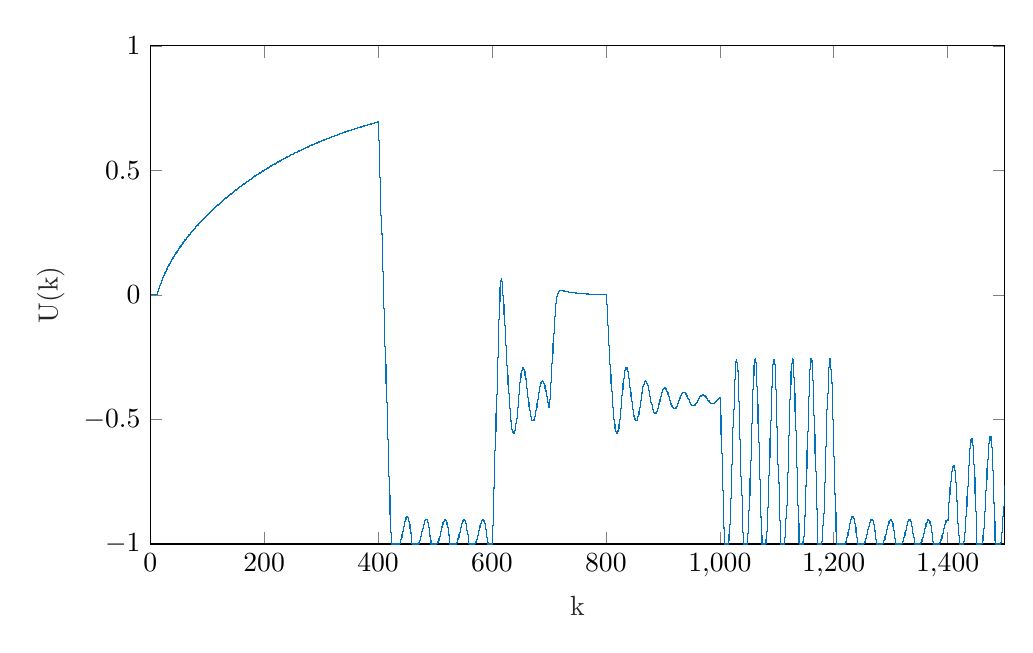
\begin{tikzpicture}

\begin{axis}[%
width=4.272in,
height=2.491in,
at={(0.717in,0.423in)},
scale only axis,
xmin=0,
xmax=1500,
xlabel style={font=\color{white!15!black}},
xlabel={k},
ymin=-1,
ymax=1,
ylabel style={font=\color{white!15!black}},
ylabel={U(k)},
axis background/.style={fill=white}
]
\addplot[const plot, color=mycolor1, forget plot] table[row sep=crcr] {%
1	0\\
2	0\\
3	0\\
4	0\\
5	0\\
6	0\\
7	0\\
8	0\\
9	0\\
10	0\\
11	0\\
12	0.00656849183014698\\
13	0.0130911837087277\\
14	0.0195673950876718\\
15	0.0259969702998995\\
16	0.0323800145904109\\
17	0.0387042185680304\\
18	0.0449369274979165\\
19	0.0510442604782427\\
20	0.057002334290044\\
21	0.062799354340218\\
22	0.0684332305765869\\
23	0.0739081327232012\\
24	0.0792315913565295\\
25	0.0844125419802625\\
26	0.0894601782058149\\
27	0.0943833550299188\\
28	0.0991903091287931\\
29	0.103888588355804\\
30	0.108485051256961\\
31	0.112985910646188\\
32	0.117396794256529\\
33	0.121722808738929\\
34	0.125968600432528\\
35	0.130138410055148\\
36	0.134236120550462\\
37	0.138265298368167\\
38	0.142229228889883\\
39	0.146130946830076\\
40	0.14997326240422\\
41	0.153758783958307\\
42	0.15748993764196\\
43	0.161168984603206\\
44	0.164798036094043\\
45	0.168379066803372\\
46	0.171913926675932\\
47	0.175404351430027\\
48	0.178851971950458\\
49	0.182258322704114\\
50	0.185624849302421\\
51	0.188952915315944\\
52	0.192243808430997\\
53	0.195498746025287\\
54	0.198718880229026\\
55	0.201905302528926\\
56	0.205059047965038\\
57	0.2081810989639\\
58	0.211272388846092\\
59	0.214333805041556\\
60	0.217366192042063\\
61	0.220370354116749\\
62	0.223347057813633\\
63	0.226297034267438\\
64	0.229220981331804\\
65	0.232119565551951\\
66	0.234993423992199\\
67	0.237843165931166\\
68	0.240669374436193\\
69	0.24347260782733\\
70	0.246253401040202\\
71	0.249012266896145\\
72	0.251749697287206\\
73	0.254466164282847\\
74	0.257162121164567\\
75	0.259838003394087\\
76	0.262494229520214\\
77	0.265131202029034\\
78	0.267749308141695\\
79	0.270348920563643\\
80	0.272930398188862\\
81	0.27549408676234\\
82	0.278040319503744\\
83	0.280569417695016\\
84	0.283081691234388\\
85	0.285577439159109\\
86	0.288056950139006\\
87	0.290520502942816\\
88	0.292968366879078\\
89	0.295400802213262\\
90	0.297818060562644\\
91	0.300220385270348\\
92	0.302608011759875\\
93	0.304981167871319\\
94	0.307340074180405\\
95	0.309684944301389\\
96	0.312015985174797\\
97	0.314333397340896\\
98	0.316637375199743\\
99	0.318928107258599\\
100	0.321205776367426\\
101	0.323470559943149\\
102	0.325722630183332\\
103	0.327962154269836\\
104	0.330189294563039\\
105	0.332404208787114\\
106	0.334607050206864\\
107	0.336797967796567\\
108	0.338977106401245\\
109	0.341144606890782\\
110	0.343300606307227\\
111	0.345445238005679\\
112	0.347578631789044\\
113	0.349700914037005\\
114	0.35181220782948\\
115	0.353912633064847\\
116	0.356002306573204\\
117	0.358081342224894\\
118	0.360149851034538\\
119	0.362207941260784\\
120	0.364255718501985\\
121	0.366293285787993\\
122	0.368320743668257\\
123	0.370338190296391\\
124	0.372345721511387\\
125	0.374343430915615\\
126	0.376331409949768\\
127	0.378309747964879\\
128	0.380278532291552\\
129	0.382237848306526\\
130	0.384187779496695\\
131	0.386128407520679\\
132	0.388059812268089\\
133	0.389982071916537\\
134	0.391895262986538\\
135	0.393799460394355\\
136	0.395694737502894\\
137	0.397581166170731\\
138	0.399458816799342\\
139	0.401327758378612\\
140	0.403188058530702\\
141	0.405039783552332\\
142	0.406882998455547\\
143	0.408717767007036\\
144	0.410544151766046\\
145	0.412362214120966\\
146	0.414172014324616\\
147	0.415973611528308\\
148	0.417767063814715\\
149	0.419552428229607\\
150	0.421329760812479\\
151	0.423099116626141\\
152	0.42486054978528\\
153	0.426614113484061\\
154	0.428359860022781\\
155	0.430097840833628\\
156	0.431828106505568\\
157	0.4335507068084\\
158	0.435265690716006\\
159	0.436973106428825\\
160	0.438673001395585\\
161	0.440365422334312\\
162	0.442050415252655\\
163	0.443728025467532\\
164	0.445398297624147\\
165	0.447061275714378\\
166	0.448717003094568\\
167	0.45036552250275\\
168	0.452006876075301\\
169	0.453641105363075\\
170	0.45526825134701\\
171	0.456888354453237\\
172	0.458501454567716\\
173	0.460107591050392\\
174	0.46170680274892\\
175	0.463299128011944\\
176	0.464884604701967\\
177	0.466463270207806\\
178	0.468035161456673\\
179	0.469600314925865\\
180	0.471158766654096\\
181	0.472710552252481\\
182	0.474255706915172\\
183	0.475794265429674\\
184	0.47732626218684\\
185	0.478851731190554\\
186	0.480370706067131\\
187	0.481883220074415\\
188	0.483389306110613\\
189	0.484888996722848\\
190	0.486382324115466\\
191	0.487869320158082\\
192	0.489350016393388\\
193	0.490824444044725\\
194	0.49229263402343\\
195	0.493754616935959\\
196	0.495210423090803\\
197	0.496660082505191\\
198	0.498103624911603\\
199	0.499541079764079\\
200	0.500972476244353\\
201	0.5023978432678\\
202	0.503817209489203\\
203	0.505230603308364\\
204	0.506638052875541\\
205	0.508039586096723\\
206	0.509435230638767\\
207	0.510825013934364\\
208	0.512208963186882\\
209	0.513587105375055\\
210	0.51495946725754\\
211	0.516326075377346\\
212	0.517686956066132\\
213	0.519042135448385\\
214	0.520391639445476\\
215	0.521735493779601\\
216	0.523073723977611\\
217	0.524406355374731\\
218	0.525733413118179\\
219	0.527054922170673\\
220	0.528370907313851\\
221	0.529681393151585\\
222	0.530986404113211\\
223	0.532285964456657\\
224	0.533580098271499\\
225	0.534868829481917\\
226	0.536152181849579\\
227	0.537430178976441\\
228	0.538702844307474\\
229	0.539970201133308\\
230	0.541232272592809\\
231	0.542489081675589\\
232	0.543740651224439\\
233	0.544987003937701\\
234	0.546228162371576\\
235	0.547464148942366\\
236	0.548694985928661\\
237	0.549920695473461\\
238	0.551141299586246\\
239	0.552356820144989\\
240	0.553567278898113\\
241	0.554772697466402\\
242	0.555973097344853\\
243	0.55716849990449\\
244	0.558358926394119\\
245	0.559544397942044\\
246	0.560724935557737\\
247	0.561900560133465\\
248	0.56307129244587\\
249	0.564237153157517\\
250	0.565398162818394\\
251	0.56655434186738\\
252	0.567705710633667\\
253	0.568852289338159\\
254	0.569994098094819\\
255	0.571131156912\\
256	0.572263485693725\\
257	0.57339110424095\\
258	0.574514032252786\\
259	0.575632289327695\\
260	0.576745894964654\\
261	0.577854868564291\\
262	0.578959229429998\\
263	0.580058996769009\\
264	0.581154189693458\\
265	0.582244827221406\\
266	0.583330928277852\\
267	0.584412511695711\\
268	0.585489596216772\\
269	0.586562200492637\\
270	0.587630343085632\\
271	0.588694042469701\\
272	0.589753317031279\\
273	0.59080818507014\\
274	0.591858664800233\\
275	0.592904774350495\\
276	0.593946531765643\\
277	0.594983955006955\\
278	0.596017061953029\\
279	0.59704587040052\\
280	0.598070398064877\\
281	0.599090662581044\\
282	0.60010668150416\\
283	0.601118472310239\\
284	0.602126052396833\\
285	0.603129439083686\\
286	0.60412864961337\\
287	0.605123701151909\\
288	0.606114610789393\\
289	0.607101395540573\\
290	0.60808407234545\\
291	0.609062658069846\\
292	0.610037169505973\\
293	0.611007623372977\\
294	0.611974036317486\\
295	0.612936424914135\\
296	0.613894805666086\\
297	0.614849195005543\\
298	0.615799609294245\\
299	0.61674606482396\\
300	0.617688577816969\\
301	0.61862716442653\\
302	0.619561840737353\\
303	0.620492622766045\\
304	0.621419526461563\\
305	0.622342567705652\\
306	0.623261762313274\\
307	0.624177126033036\\
308	0.625088674547601\\
309	0.625996423474101\\
310	0.626900388364539\\
311	0.627800584706183\\
312	0.628697027921957\\
313	0.629589733370822\\
314	0.630478716348154\\
315	0.631363992086112\\
316	0.632245575754006\\
317	0.633123482458651\\
318	0.633997727244728\\
319	0.634868325095122\\
320	0.635735290931275\\
321	0.636598639613514\\
322	0.637458385941391\\
323	0.638314544654008\\
324	0.639167130430339\\
325	0.640016157889548\\
326	0.640861641591309\\
327	0.641703596036106\\
328	0.642542035665549\\
329	0.643376974862667\\
330	0.644208427952209\\
331	0.645036409200939\\
332	0.645860932817922\\
333	0.646682012954813\\
334	0.647499663706139\\
335	0.648313899109578\\
336	0.649124733146231\\
337	0.649932179740902\\
338	0.650736252762359\\
339	0.651536966023605\\
340	0.65233433328214\\
341	0.653128368240218\\
342	0.653919084545108\\
343	0.654706495789345\\
344	0.655490615510983\\
345	0.656271457193845\\
346	0.657049034267766\\
347	0.657823360108836\\
348	0.658594448039648\\
349	0.659362311329526\\
350	0.66012696319477\\
351	0.660888416798887\\
352	0.66164668525282\\
353	0.662401781615183\\
354	0.663153718892482\\
355	0.663902510039346\\
356	0.664648167958745\\
357	0.665390705502218\\
358	0.666130135470083\\
359	0.666866470611662\\
360	0.667599723625495\\
361	0.66832990715955\\
362	0.66905703381144\\
363	0.669781116128629\\
364	0.670502166608642\\
365	0.671220197699275\\
366	0.671935221798793\\
367	0.672647251256141\\
368	0.673356298371142\\
369	0.6740623753947\\
370	0.674765494528996\\
371	0.675465667927689\\
372	0.67616290769611\\
373	0.676857225891458\\
374	0.677548634522994\\
375	0.678237145552231\\
376	0.67892277089313\\
377	0.679605522412282\\
378	0.680285411929103\\
379	0.68096245121602\\
380	0.681636651998652\\
381	0.682308025956003\\
382	0.682976584720639\\
383	0.683642339878875\\
384	0.684305302970952\\
385	0.684965485491224\\
386	0.685622898888329\\
387	0.686277554565376\\
388	0.686929463880114\\
389	0.687578638145115\\
390	0.688225088627947\\
391	0.688868826551347\\
392	0.689509863093395\\
393	0.690148209387689\\
394	0.690783876523511\\
395	0.691416875546006\\
396	0.692047217456343\\
397	0.692674913211891\\
398	0.69329997372638\\
399	0.693922409870077\\
400	0.694542232469945\\
401	0.619542232469945\\
402	0.544542232469945\\
403	0.469542232469945\\
404	0.394542232469945\\
405	0.319542232469945\\
406	0.244542232469945\\
407	0.169542232469945\\
408	0.0945422324699451\\
409	0.0195422324699451\\
410	-0.0554577675300549\\
411	-0.130457767530055\\
412	-0.205457767530055\\
413	-0.280457767530055\\
414	-0.355457767530055\\
415	-0.430457767530055\\
416	-0.505457767530055\\
417	-0.580457767530055\\
418	-0.655457767530055\\
419	-0.730457767530055\\
420	-0.805457767530055\\
421	-0.880457767530055\\
422	-0.955457767530055\\
423	-1\\
424	-1\\
425	-1\\
426	-1\\
427	-1\\
428	-1\\
429	-1\\
430	-1\\
431	-1\\
432	-1\\
433	-1\\
434	-1\\
435	-1\\
436	-1\\
437	-1\\
438	-0.996854506661506\\
439	-0.990930901664204\\
440	-0.982922587183526\\
441	-0.973388908553367\\
442	-0.962773329995785\\
443	-0.95147051379859\\
444	-0.939883298750177\\
445	-0.928446712883258\\
446	-0.917629422127481\\
447	-0.907922574394113\\
448	-0.899822212705854\\
449	-0.893808450145619\\
450	-0.890322989016894\\
451	-0.889746023881842\\
452	-0.892373565942176\\
453	-0.898396391507356\\
454	-0.907881942772113\\
455	-0.920760499133069\\
456	-0.936816761350377\\
457	-0.95568766116423\\
458	-0.976866771727386\\
459	-0.99971522121187\\
460	-1\\
461	-1\\
462	-1\\
463	-1\\
464	-1\\
465	-1\\
466	-1\\
467	-1\\
468	-1\\
469	-1\\
470	-0.999140658407652\\
471	-0.996051594617867\\
472	-0.991090179404695\\
473	-0.984585985045346\\
474	-0.976833431361376\\
475	-0.968102260890142\\
476	-0.958671631760738\\
477	-0.94885354791598\\
478	-0.938999472914118\\
479	-0.929496167246454\\
480	-0.920755127297951\\
481	-0.913198276168055\\
482	-0.907241296762243\\
483	-0.903275408469468\\
484	-0.901648269809515\\
485	-0.902644793048533\\
486	-0.906468813681572\\
487	-0.913226673215738\\
488	-0.922913799620548\\
489	-0.935405284945689\\
490	-0.950451263008838\\
491	-0.967677600825985\\
492	-0.986592073855703\\
493	-1\\
494	-1\\
495	-1\\
496	-1\\
497	-1\\
498	-1\\
499	-1\\
500	-1\\
501	-1\\
502	-1\\
503	-0.999462142062378\\
504	-0.996723868759006\\
505	-0.992114214996992\\
506	-0.985944329523515\\
507	-0.97849754302294\\
508	-0.970032808685077\\
509	-0.96081706901427\\
510	-0.951149608746157\\
511	-0.941369755650998\\
512	-0.931853700519672\\
513	-0.923004754874192\\
514	-0.91523973116161\\
515	-0.90897286265253\\
516	-0.904598059061172\\
517	-0.902470149719789\\
518	-0.902885858086923\\
519	-0.906065409370204\\
520	-0.912135799969016\\
521	-0.921116802693669\\
522	-0.932910721320182\\
523	-0.947296737211373\\
524	-0.963930423741162\\
525	-0.982348674500882\\
526	-1\\
527	-1\\
528	-1\\
529	-1\\
530	-1\\
531	-1\\
532	-1\\
533	-1\\
534	-1\\
535	-1\\
536	-0.999873045875112\\
537	-0.99749163025508\\
538	-0.993185162837048\\
539	-0.987267837045163\\
540	-0.980027585476198\\
541	-0.971722326062297\\
542	-0.962613020755498\\
543	-0.952991155392444\\
544	-0.943188547229676\\
545	-0.933575466483647\\
546	-0.924551673394621\\
547	-0.916533299804052\\
548	-0.909937121497686\\
549	-0.905163053205527\\
550	-0.902575504400615\\
551	-0.902484308981058\\
552	-0.905126102113805\\
553	-0.910647157050566\\
554	-0.919088758199904\\
555	-0.930376147004133\\
556	-0.944311926222516\\
557	-0.960574556680135\\
558	-0.978722258352289\\
559	-0.998202280846966\\
560	-1\\
561	-1\\
562	-1\\
563	-1\\
564	-1\\
565	-1\\
566	-1\\
567	-1\\
568	-1\\
569	-1\\
570	-0.998030980591595\\
571	-0.994073280291696\\
572	-0.988445233630392\\
573	-0.981440557162503\\
574	-0.973321732626992\\
575	-0.964348107793261\\
576	-0.954805089810103\\
577	-0.945017071771462\\
578	-0.935347576221501\\
579	-0.926191503664134\\
580	-0.917962727186993\\
581	-0.911078815221918\\
582	-0.905943827388254\\
583	-0.902929846162467\\
584	-0.902357939234821\\
585	-0.904479396562147\\
586	-0.909458232600421\\
587	-0.917356023853365\\
588	-0.928120132457782\\
589	-0.941576236277385\\
590	-0.957425851816696\\
591	-0.975249224584386\\
592	-0.994513615894961\\
593	-1\\
594	-1\\
595	-1\\
596	-1\\
597	-1\\
598	-1\\
599	-1\\
600	-1\\
601	-0.925\\
602	-0.85\\
603	-0.775\\
604	-0.7\\
605	-0.625\\
606	-0.55\\
607	-0.475\\
608	-0.4\\
609	-0.325\\
610	-0.25\\
611	-0.175\\
612	-0.1\\
613	-0.0250000000000002\\
614	0.027602713657995\\
615	0.0570738453770082\\
616	0.0652668944077882\\
617	0.0554849691754414\\
618	0.0320188798979265\\
619	-0.000634996907724381\\
620	-0.0386746482127763\\
621	-0.079415068438552\\
622	-0.121201263111646\\
623	-0.163095252011474\\
624	-0.204566269684066\\
625	-0.245271893272029\\
626	-0.284930853602743\\
627	-0.323260081438226\\
628	-0.359949355646756\\
629	-0.394655766208351\\
630	-0.42700818310358\\
631	-0.456617123626723\\
632	-0.483087807451069\\
633	-0.506035308483216\\
634	-0.525101052063066\\
635	-0.539969988286401\\
636	-0.550387799822231\\
637	-0.556177531490771\\
638	-0.557255053822923\\
639	-0.553642777645532\\
640	-0.545481013484024\\
641	-0.533036321007367\\
642	-0.516706129889273\\
643	-0.497018847785599\\
644	-0.474628618835837\\
645	-0.450303875580719\\
646	-0.424908864906449\\
647	-0.399377467353492\\
648	-0.374678938333678\\
649	-0.351775782479868\\
650	-0.331574953020042\\
651	-0.314875034964543\\
652	-0.302313948758156\\
653	-0.294323589710188\\
654	-0.291098868945047\\
655	-0.292587816254353\\
656	-0.298506140926919\\
657	-0.308374461718761\\
658	-0.321571126695331\\
659	-0.337390377440379\\
660	-0.355095846155526\\
661	-0.373962561312088\\
662	-0.393305046558316\\
663	-0.412492881485937\\
664	-0.430957219272251\\
665	-0.448192187756881\\
666	-0.463754407898187\\
667	-0.477262729662464\\
668	-0.48839920105231\\
669	-0.496911479487112\\
670	-0.50261639824816\\
671	-0.505404148870742\\
672	-0.505242445016026\\
673	-0.502180021596541\\
674	-0.496348848203557\\
675	-0.48796447517841\\
676	-0.477323977520005\\
677	-0.464801019977984\\
678	-0.450837645944886\\
679	-0.435932506777811\\
680	-0.420625413222066\\
681	-0.405478323933618\\
682	-0.391053202134812\\
683	-0.377887573937505\\
684	-0.366469091057026\\
685	-0.357210877626985\\
686	-0.350429817296399\\
687	-0.346330064074389\\
688	-0.344993791238345\\
689	-0.346380453911928\\
690	-0.350334707207177\\
691	-0.356601838065378\\
692	-0.364848483741385\\
693	-0.374685835159283\\
694	-0.385692595168388\\
695	-0.397435586647747\\
696	-0.409486821576844\\
697	-0.421436748928622\\
698	-0.432904075748964\\
699	-0.443542914198594\\
700	-0.453048076620343\\
701	-0.420106139655323\\
702	-0.385844371306655\\
703	-0.350106277061664\\
704	-0.312786002736977\\
705	-0.273832089502674\\
706	-0.233754837572822\\
707	-0.193614481823422\\
708	-0.154747747485357\\
709	-0.118504800248216\\
710	-0.0860508683491354\\
711	-0.0582257578674364\\
712	-0.0354554189995927\\
713	-0.0177250194307122\\
714	-0.00462554010609987\\
715	0.00453203372633672\\
716	0.0105667860153288\\
717	0.0142867853816173\\
718	0.0163915551508201\\
719	0.0174283317900594\\
720	0.017791933469569\\
721	0.017749288317062\\
722	0.0174717565465327\\
723	0.0170649530498263\\
724	0.016591921104669\\
725	0.0160893296103454\\
726	0.0155780194625879\\
727	0.0150695480012024\\
728	0.0145701219005565\\
729	0.0140829112966882\\
730	0.013609391574109\\
731	0.0131501117558673\\
732	0.0127051285965692\\
733	0.0122742476318021\\
734	0.0118571540265846\\
735	0.0114534814969266\\
736	0.0110628471646566\\
737	0.0106848681889531\\
738	0.0103191690015813\\
739	0.00996538393399065\\
740	0.00962315774612125\\
741	0.00929214531456316\\
742	0.00897201107140951\\
743	0.00866242844486632\\
744	0.00836307938825205\\
745	0.00807365401088976\\
746	0.00779385029640336\\
747	0.0075233738867611\\
748	0.00726193791181244\\
749	0.00700926284821968\\
750	0.00676507639607008\\
751	0.00652911336514229\\
752	0.00630111556559432\\
753	0.00608083169982457\\
754	0.00586801725360607\\
755	0.00566243438547854\\
756	0.00546385181394481\\
757	0.00527204470236405\\
758	0.00508679454163927\\
759	0.0049078890309124\\
760	0.00473512195653976\\
761	0.00456829306964716\\
762	0.00440720796256959\\
763	0.00425167794447467\\
764	0.00410151991645706\\
765	0.00395655624637516\\
766	0.00381661464368448\\
767	0.00368152803450426\\
768	0.00355113443713652\\
769	0.00342527683823923\\
770	0.00330380306983919\\
771	0.00318656568735384\\
772	0.0030734218487764\\
773	0.00296423319516428\\
774	0.00285886573255694\\
775	0.00275718971543657\\
776	0.00265907953183277\\
777	0.00256441359016079\\
778	0.00247307420787228\\
779	0.00238494750198731\\
780	0.00229992328156669\\
781	0.00221789494217515\\
782	0.00213875936237737\\
783	0.00206241680230115\\
784	0.00198877080429503\\
785	0.00191772809570085\\
786	0.00184919849375562\\
787	0.00178309481263159\\
788	0.00171933277261781\\
789	0.00165783091144224\\
790	0.00159851049772838\\
791	0.00154129544657711\\
792	0.00148611223726027\\
793	0.00143288983300942\\
794	0.00138155960288019\\
795	0.00133205524567004\\
796	0.00128431271586469\\
797	0.00123827015158647\\
798	0.00119386780451587\\
799	0.00115104797175602\\
800	0.00110975492960823\\
801	-0.0399831390691931\\
802	-0.080788362345438\\
803	-0.121301711638529\\
804	-0.161522262461323\\
805	-0.201450719351627\\
806	-0.241002864076264\\
807	-0.279915589944882\\
808	-0.317828784978161\\
809	-0.354346347954415\\
810	-0.389061594957614\\
811	-0.421564341152483\\
812	-0.451443493140572\\
813	-0.478292139402557\\
814	-0.501716980825748\\
815	-0.521351441803555\\
816	-0.536871073945989\\
817	-0.548009853961352\\
818	-0.554576581252069\\
819	-0.556470246151657\\
820	-0.553693836635565\\
821	-0.546365943693121\\
822	-0.53472950953131\\
823	-0.519157009573406\\
824	-0.500151296416841\\
825	-0.478341281544799\\
826	-0.454471606418714\\
827	-0.429385483328795\\
828	-0.404000007101119\\
829	-0.379273514791243\\
830	-0.356165097094194\\
831	-0.335587261845419\\
832	-0.318354112917196\\
833	-0.30512919776366\\
834	-0.296379055298134\\
835	-0.292339718093246\\
836	-0.293002991609074\\
837	-0.298126543579227\\
838	-0.307266993930965\\
839	-0.319829884336445\\
840	-0.335126816159178\\
841	-0.352429661893811\\
842	-0.371014444869244\\
843	-0.390191713756441\\
844	-0.409324153526714\\
845	-0.427834586590841\\
846	-0.445208225715906\\
847	-0.460992524505291\\
848	-0.47479690439409\\
849	-0.486293544114024\\
850	-0.495219568343015\\
851	-0.501380428669108\\
852	-0.504653981083172\\
853	-0.504994644977987\\
854	-0.502437003830044\\
855	-0.497098226899734\\
856	-0.48917872788688\\
857	-0.47896052154908\\
858	-0.466802794954645\\
859	-0.453134285034322\\
860	-0.438442161275193\\
861	-0.423257267409336\\
862	-0.408135795716024\\
863	-0.393637766959573\\
864	-0.380303073853437\\
865	-0.36862630121916\\
866	-0.359032010624043\\
867	-0.351852572566271\\
868	-0.347310803914822\\
869	-0.345509473669044\\
870	-0.346429087544692\\
871	-0.349934297546868\\
872	-0.355788021135504\\
873	-0.363671228809708\\
874	-0.373205691428077\\
875	-0.383976938925719\\
876	-0.395555216287263\\
877	-0.407513094724236\\
878	-0.419439308389225\\
879	-0.430949103337818\\
880	-0.441691795710884\\
881	-0.451356351071188\\
882	-0.459675700099748\\
883	-0.466430299635057\\
884	-0.471451216410591\\
885	-0.474622805878979\\
886	-0.475884902773993\\
887	-0.47523433637487\\
888	-0.472725525001679\\
889	-0.468469881972276\\
890	-0.462633771652276\\
891	-0.455434785016974\\
892	-0.447136158064351\\
893	-0.438039234440395\\
894	-0.428473977716678\\
895	-0.418787670247722\\
896	-0.409332093147785\\
897	-0.40044965922921\\
898	-0.392459153471125\\
899	-0.385641899700034\\
900	-0.380229284262431\\
901	-0.376392589426814\\
902	-0.374235988091224\\
903	-0.373793312961152\\
904	-0.375028855101576\\
905	-0.37784202217225\\
906	-0.382075276203686\\
907	-0.387524459379986\\
908	-0.393950465599334\\
909	-0.401091243487151\\
910	-0.408673293622568\\
911	-0.416422086427932\\
912	-0.424071105714606\\
913	-0.431369457805759\\
914	-0.438088144893713\\
915	-0.444025178038878\\
916	-0.449009713566933\\
917	-0.452905359320334\\
918	-0.455612737504103\\
919	-0.457071327324414\\
920	-0.457260555533829\\
921	-0.456200062995422\\
922	-0.453949053091638\\
923	-0.450604623592447\\
924	-0.446298996836649\\
925	-0.441195592877981\\
926	-0.435483935639925\\
927	-0.429373441866106\\
928	-0.423086214731743\\
929	-0.416849044952412\\
930	-0.410884906543851\\
931	-0.405404313929717\\
932	-0.400596971197527\\
933	-0.396624180635178\\
934	-0.393612474213723\\
935	-0.391648879675805\\
936	-0.390778130292439\\
937	-0.391001981485123\\
938	-0.392280625669269\\
939	-0.394536023688477\\
940	-0.39765682410214\\
941	-0.401504442815535\\
942	-0.405919837155587\\
943	-0.41073052943475\\
944	-0.415757502461239\\
945	-0.420821683337277\\
946	-0.425749831030035\\
947	-0.430379730335108\\
948	-0.434564659552909\\
949	-0.438177138259812\\
950	-0.441111977502025\\
951	-0.443288653489046\\
952	-0.444653014477345\\
953	-0.445178315593638\\
954	-0.444865563083945\\
955	-0.443743141540071\\
956	-0.441865697264368\\
957	-0.439312259163391\\
958	-0.43618359563156\\
959	-0.43259883133942\\
960	-0.428691380596256\\
961	-0.424604292259527\\
962	-0.420485142485439\\
963	-0.416480652572272\\
964	-0.412731245528092\\
965	-0.409365781980869\\
966	-0.406496728713921\\
967	-0.404216007186856\\
968	-0.402591742254084\\
969	-0.40166608286726\\
970	-0.401454200025774\\
971	-0.401944489063983\\
972	-0.403099922461581\\
973	-0.404860425608305\\
974	-0.407146090216028\\
975	-0.40986100438805\\
976	-0.412897466779584\\
977	-0.416140362740267\\
978	-0.419471507480228\\
979	-0.422773798073834\\
980	-0.425935055396566\\
981	-0.42885147310111\\
982	-0.431430619810656\\
983	-0.433593961417021\\
984	-0.435278883180482\\
985	-0.436440197964132\\
986	-0.437051129734608\\
987	-0.43710376282562\\
988	-0.436608949493119\\
989	-0.435595672598313\\
990	-0.434109867880115\\
991	-0.432212721706568\\
992	-0.42997847538399\\
993	-0.427491785520421\\
994	-0.424844710590224\\
995	-0.422133415298372\\
996	-0.41945470478092\\
997	-0.416902517999283\\
998	-0.414564521664264\\
999	-0.412518950556362\\
1000	-0.410831835519856\\
1001	-0.485831835519856\\
1002	-0.560831835519856\\
1003	-0.635831835519856\\
1004	-0.710831835519856\\
1005	-0.785831835519856\\
1006	-0.860831835519856\\
1007	-0.935831835519856\\
1008	-1\\
1009	-1\\
1010	-1\\
1011	-1\\
1012	-1\\
1013	-1\\
1014	-1\\
1015	-0.987635870172822\\
1016	-0.961650029606116\\
1017	-0.923450430226157\\
1018	-0.874595020344178\\
1019	-0.816653985526071\\
1020	-0.751306189219481\\
1021	-0.680497458248094\\
1022	-0.606534665492556\\
1023	-0.532113114962388\\
1024	-0.460291035535514\\
1025	-0.394418888147141\\
1026	-0.338022433340466\\
1027	-0.294629431559193\\
1028	-0.267522060116705\\
1029	-0.259399000468602\\
1030	-0.2719636443821\\
1031	-0.305533335285714\\
1032	-0.358846972847021\\
1033	-0.429225199134884\\
1034	-0.504225199134884\\
1035	-0.579225199134884\\
1036	-0.654225199134884\\
1037	-0.729225199134884\\
1038	-0.804225199134884\\
1039	-0.879225199134884\\
1040	-0.954225199134884\\
1041	-1\\
1042	-1\\
1043	-1\\
1044	-1\\
1045	-1\\
1046	-1\\
1047	-1\\
1048	-0.98541766219494\\
1049	-0.957030640795684\\
1050	-0.916440844181003\\
1051	-0.865328454231867\\
1052	-0.805334606697302\\
1053	-0.738207632967161\\
1054	-0.66597667416337\\
1055	-0.591041560730564\\
1056	-0.516193446747586\\
1057	-0.444581640813642\\
1058	-0.379634396225743\\
1059	-0.324931466927721\\
1060	-0.28401633898207\\
1061	-0.260128426596417\\
1062	-0.255840937212288\\
1063	-0.272632454953168\\
1064	-0.310509325152281\\
1065	-0.367870966753575\\
1066	-0.441753314804485\\
1067	-0.516753314804485\\
1068	-0.591753314804485\\
1069	-0.666753314804485\\
1070	-0.741753314804484\\
1071	-0.816753314804484\\
1072	-0.891753314804484\\
1073	-0.966753314804484\\
1074	-1\\
1075	-1\\
1076	-1\\
1077	-1\\
1078	-1\\
1079	-1\\
1080	-0.997953660103689\\
1081	-0.980950424196584\\
1082	-0.950397780304831\\
1083	-0.907921977620278\\
1084	-0.855203884431998\\
1085	-0.793900238215\\
1086	-0.725803118697637\\
1087	-0.653003050542141\\
1088	-0.578003050542141\\
1089	-0.503585054383891\\
1090	-0.432986484191647\\
1091	-0.369667903586746\\
1092	-0.317212630970488\\
1093	-0.279125860148913\\
1094	-0.258552314863955\\
1095	-0.257899759684662\\
1096	-0.278409644004443\\
1097	-0.319808796008359\\
1098	-0.380235692211134\\
1099	-0.455235692211134\\
1100	-0.530235692211134\\
1101	-0.605235692211134\\
1102	-0.680235692211134\\
1103	-0.755235692211134\\
1104	-0.830235692211134\\
1105	-0.905235692211134\\
1106	-0.980235692211134\\
1107	-1\\
1108	-1\\
1109	-1\\
1110	-1\\
1111	-1\\
1112	-1\\
1113	-0.995125006274957\\
1114	-0.975516452600245\\
1115	-0.942640797248549\\
1116	-0.898147361360919\\
1117	-0.843715541832924\\
1118	-0.781026924480324\\
1119	-0.711929419427579\\
1120	-0.638585010982371\\
1121	-0.563585010982371\\
1122	-0.489753055284319\\
1123	-0.420394213346206\\
1124	-0.358999944508835\\
1125	-0.309150472670054\\
1126	-0.274299300670835\\
1127	-0.257473706126487\\
1128	-0.260883643731452\\
1129	-0.285496236261368\\
1130	-0.330727040365783\\
1131	-0.39443747471686\\
1132	-0.46943747471686\\
1133	-0.54443747471686\\
1134	-0.61943747471686\\
1135	-0.69443747471686\\
1136	-0.76943747471686\\
1137	-0.844437474716859\\
1138	-0.919437474716859\\
1139	-0.994437474716859\\
1140	-1\\
1141	-1\\
1142	-1\\
1143	-1\\
1144	-1\\
1145	-1\\
1146	-0.99209205245223\\
1147	-0.969694393668878\\
1148	-0.934334883520445\\
1149	-0.887686289081397\\
1150	-0.831425545764904\\
1151	-0.767260801608363\\
1152	-0.697100284637034\\
1153	-0.623183311617148\\
1154	-0.548183311617148\\
1155	-0.474995736831967\\
1156	-0.406984820290829\\
1157	-0.347674259680444\\
1158	-0.300638534611952\\
1159	-0.269271100616637\\
1160	-0.256465425743896\\
1161	-0.264209326862034\\
1162	-0.293168214228647\\
1163	-0.342425171685877\\
1164	-0.40955698663484\\
1165	-0.48455698663484\\
1166	-0.55955698663484\\
1167	-0.63455698663484\\
1168	-0.70955698663484\\
1169	-0.78455698663484\\
1170	-0.85955698663484\\
1171	-0.93455698663484\\
1172	-1\\
1173	-1\\
1174	-1\\
1175	-1\\
1176	-1\\
1177	-1\\
1178	-1\\
1179	-0.989104960655216\\
1180	-0.964008289274349\\
1181	-0.926278445270593\\
1182	-0.87759698616702\\
1183	-0.819628644191756\\
1184	-0.75410181550314\\
1185	-0.68298024818109\\
1186	-0.60857619849157\\
1187	-0.533588888386472\\
1188	-0.461084902558459\\
1189	-0.394430514114147\\
1190	-0.337176545133313\\
1191	-0.292886361941764\\
1192	-0.264888948193366\\
1193	-0.25593961639707\\
1194	-0.267802324095081\\
1195	-0.300847108543143\\
1196	-0.353843497659603\\
1197	-0.424112724082367\\
1198	-0.499112724082367\\
1199	-0.574112724082367\\
1200	-0.649112724082367\\
1201	-0.724112724082367\\
1202	-0.799112724082367\\
1203	-0.874112724082367\\
1204	-0.949112724082367\\
1205	-1\\
1206	-1\\
1207	-1\\
1208	-1\\
1209	-1\\
1210	-1\\
1211	-1\\
1212	-1\\
1213	-1\\
1214	-1\\
1215	-1\\
1216	-1\\
1217	-1\\
1218	-1\\
1219	-1\\
1220	-0.99738469532889\\
1221	-0.991846061047147\\
1222	-0.984108354960221\\
1223	-0.974756782383589\\
1224	-0.964256173646032\\
1225	-0.953010210469449\\
1226	-0.941421745426591\\
1227	-0.929922504086852\\
1228	-0.918977884090803\\
1229	-0.909077564487615\\
1230	-0.900718730882136\\
1231	-0.894385600687009\\
1232	-0.890527070234809\\
1233	-0.889533599167481\\
1234	-0.891714369041311\\
1235	-0.897275899315962\\
1236	-0.906303439366063\\
1237	-0.918746466595256\\
1238	-0.934409467856312\\
1239	-0.952948870316558\\
1240	-0.973876560638006\\
1241	-0.996569957289582\\
1242	-1\\
1243	-1\\
1244	-1\\
1245	-1\\
1246	-1\\
1247	-1\\
1248	-1\\
1249	-1\\
1250	-1\\
1251	-1\\
1252	-0.999525255600883\\
1253	-0.996763931433724\\
1254	-0.992076256974894\\
1255	-0.985796476854009\\
1256	-0.978224605030398\\
1257	-0.969630279775798\\
1258	-0.960287705512577\\
1259	-0.95050214751178\\
1260	-0.940618571521302\\
1261	-0.931018706741026\\
1262	-0.922111199441045\\
1263	-0.914317749558184\\
1264	-0.908056747509631\\
1265	-0.903725248449241\\
1266	-0.901679954772937\\
1267	-0.902217965591757\\
1268	-0.905558211474912\\
1269	-0.91182462065086\\
1270	-0.921032106016851\\
1271	-0.933076396383488\\
1272	-0.947728556337021\\
1273	-0.964634762701493\\
1274	-0.983321567148111\\
1275	-1\\
1276	-1\\
1277	-1\\
1278	-1\\
1279	-1\\
1280	-1\\
1281	-1\\
1282	-1\\
1283	-1\\
1284	-1\\
1285	-0.999839393787096\\
1286	-0.99742413930653\\
1287	-0.993085460294635\\
1288	-0.987138641439855\\
1289	-0.97987218497885\\
1290	-0.971544735677977\\
1291	-0.962418229203118\\
1292	-0.952785214497692\\
1293	-0.942978525439563\\
1294	-0.933369298542351\\
1295	-0.924357933114874\\
1296	-0.916360912928112\\
1297	-0.90979502980197\\
1298	-0.905059840148104\\
1299	-0.9025189949516\\
1300	-0.902481159939936\\
1301	-0.905181402801968\\
1302	-0.910764062794482\\
1303	-0.919268179798246\\
1304	-0.930616517964446\\
1305	-0.944609065849584\\
1306	-0.960921641403217\\
1307	-0.979109906726222\\
1308	-0.99861875048672\\
1309	-1\\
1310	-1\\
1311	-1\\
1312	-1\\
1313	-1\\
1314	-1\\
1315	-1\\
1316	-1\\
1317	-1\\
1318	-1\\
1319	-0.997983099352548\\
1320	-0.993984400395136\\
1321	-0.988321960148535\\
1322	-0.981288970439479\\
1323	-0.973147256772697\\
1324	-0.964156209798074\\
1325	-0.954601878356852\\
1326	-0.944809517136728\\
1327	-0.935143478003524\\
1328	-0.925999304990651\\
1329	-0.917791238808293\\
1330	-0.910936883112094\\
1331	-0.905839961921536\\
1332	-0.902871826631418\\
1333	-0.902352409015815\\
1334	-0.904531467613713\\
1335	-0.909571120880776\\
1336	-0.917530738460896\\
1337	-0.928355240269608\\
1338	-0.941867720464623\\
1339	-0.957767077145364\\
1340	-0.975631015571587\\
1341	-0.994924446697002\\
1342	-1\\
1343	-1\\
1344	-1\\
1345	-1\\
1346	-1\\
1347	-1\\
1348	-1\\
1349	-1\\
1350	-1\\
1351	-1\\
1352	-0.998423936068064\\
1353	-0.994801694482222\\
1354	-0.989454292069664\\
1355	-0.982680045942717\\
1356	-0.974747031171004\\
1357	-0.96591438873111\\
1358	-0.956462372844503\\
1359	-0.946708406531809\\
1360	-0.937009300360669\\
1361	-0.927754759694097\\
1362	-0.919355714829463\\
1363	-0.912229502642693\\
1364	-0.906782973495122\\
1365	-0.903394222074837\\
1366	-0.902393624796985\\
1367	-0.904045000230313\\
1368	-0.908527859195589\\
1369	-0.915921804383206\\
1370	-0.926194138113165\\
1371	-0.93919162591016\\
1372	-0.954637146463609\\
1373	-0.972131658341614\\
1374	-0.991161571472582\\
1375	-1\\
1376	-1\\
1377	-1\\
1378	-1\\
1379	-1\\
1380	-1\\
1381	-1\\
1382	-1\\
1383	-1\\
1384	-1\\
1385	-0.998856170872317\\
1386	-0.995604093753153\\
1387	-0.990567266537099\\
1388	-0.984048725657051\\
1389	-0.976322457777381\\
1390	-0.967647221085571\\
1391	-0.958297492253344\\
1392	-0.948582934102487\\
1393	-0.938852883168953\\
1394	-0.929491237484126\\
1395	-0.920905596993492\\
1396	-0.913512953794381\\
1397	-0.90772314660209\\
1398	-0.903920817417264\\
1399	-0.902446539452541\\
1400	-0.903577902065036\\
1401	-0.866458418258381\\
1402	-0.832526921280623\\
1403	-0.801777031230317\\
1404	-0.774079864494833\\
1405	-0.749181366882621\\
1406	-0.72729779287991\\
1407	-0.709128172694075\\
1408	-0.695615949559828\\
1409	-0.687728386926095\\
1410	-0.68630635839746\\
1411	-0.691970582593675\\
1412	-0.705062468405246\\
1413	-0.725607001064131\\
1414	-0.753294330536905\\
1415	-0.787480804618536\\
1416	-0.827209697781202\\
1417	-0.871249282174554\\
1418	-0.918142991815363\\
1419	-0.966265951014582\\
1420	-1\\
1421	-1\\
1422	-1\\
1423	-1\\
1424	-1\\
1425	-1\\
1426	-1\\
1427	-1\\
1428	-0.991581516530145\\
1429	-0.975287915734454\\
1430	-0.952079121468236\\
1431	-0.922940652039977\\
1432	-0.888821983568931\\
1433	-0.850728372704232\\
1434	-0.809819504981826\\
1435	-0.767453874241617\\
1436	-0.72519086849124\\
1437	-0.684762570132539\\
1438	-0.648022933453629\\
1439	-0.616877695791566\\
1440	-0.593196236126831\\
1441	-0.578706871187004\\
1442	-0.574879488370938\\
1443	-0.582803697596804\\
1444	-0.603076149663039\\
1445	-0.635715294259747\\
1446	-0.680122114826627\\
1447	-0.73509819794755\\
1448	-0.798918642981016\\
1449	-0.869442746716081\\
1450	-0.944237694671628\\
1451	-1\\
1452	-1\\
1453	-1\\
1454	-1\\
1455	-1\\
1456	-1\\
1457	-1\\
1458	-1\\
1459	-1\\
1460	-0.997780270878274\\
1461	-0.98603797503854\\
1462	-0.966073496315359\\
1463	-0.939160339522372\\
1464	-0.906487609543224\\
1465	-0.869161540238385\\
1466	-0.828337234471158\\
1467	-0.785326563881299\\
1468	-0.741639320162875\\
1469	-0.698977358419724\\
1470	-0.659196369754482\\
1471	-0.624243812872867\\
1472	-0.596076634974174\\
1473	-0.57656046899487\\
1474	-0.567352952241253\\
1475	-0.569777265963163\\
1476	-0.584697449200325\\
1477	-0.612413030834648\\
1478	-0.652593754701792\\
1479	-0.704271433230301\\
1480	-0.765893605263092\\
1481	-0.83542688923754\\
1482	-0.91042688923754\\
1483	-0.98542688923754\\
1484	-1\\
1485	-1\\
1486	-1\\
1487	-1\\
1488	-1\\
1489	-1\\
1490	-1\\
1491	-1\\
1492	-1\\
1493	-0.992878638044821\\
1494	-0.976836656502449\\
1495	-0.953187934820158\\
1496	-0.923182143397766\\
1497	-0.887962022889933\\
1498	-0.848651046182607\\
1499	-0.806481754092297\\
1500	-0.762869068776074\\
};
\end{axis}
\end{tikzpicture}%
\caption{Regulacja DMC, $N = 15; N_u = 15; \lambda = 10$}
\end{figure}

\begin{figure}[H]
\centering
% This file was created by matlab2tikz.
%
%The latest updates can be retrieved from
%  http://www.mathworks.com/matlabcentral/fileexchange/22022-matlab2tikz-matlab2tikz
%where you can also make suggestions and rate matlab2tikz.
%
\definecolor{mycolor1}{rgb}{0.00000,0.44700,0.74100}%
\definecolor{mycolor2}{rgb}{0.85000,0.32500,0.09800}%
%
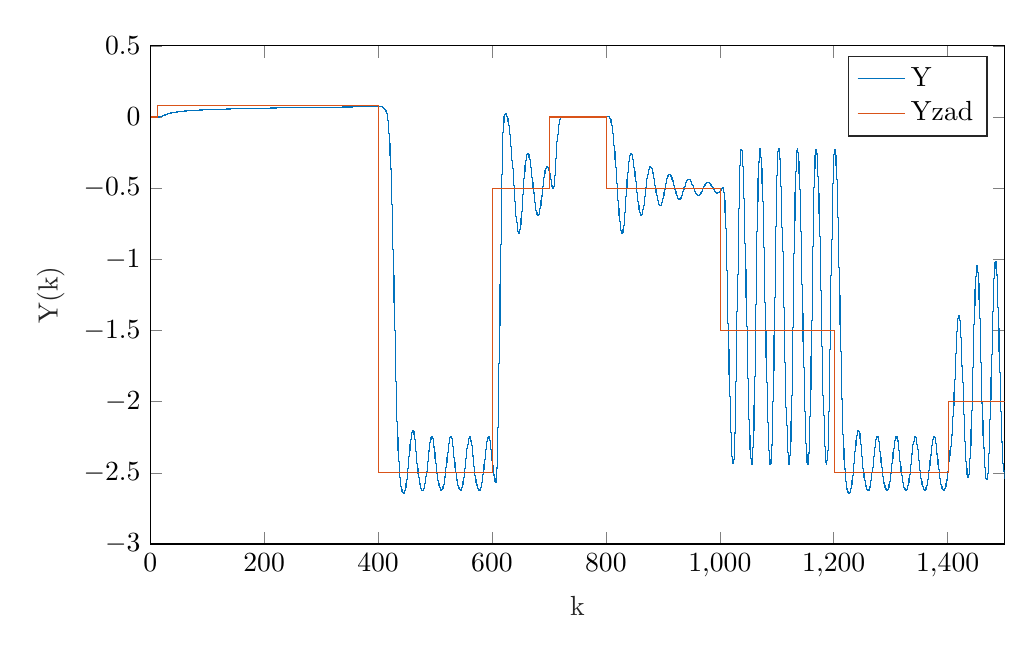
\begin{tikzpicture}

\begin{axis}[%
width=4.272in,
height=2.491in,
at={(0.717in,0.423in)},
scale only axis,
xmin=0,
xmax=1500,
xlabel style={font=\color{white!15!black}},
xlabel={k},
ymin=-3,
ymax=0.5,
ylabel style={font=\color{white!15!black}},
ylabel={Y(k)},
axis background/.style={fill=white},
legend style={legend cell align=left, align=left, draw=white!15!black}
]
\addplot[const plot, color=mycolor1] table[row sep=crcr] {%
1	0\\
2	0\\
3	0\\
4	0\\
5	0\\
6	0\\
7	0\\
8	0\\
9	0\\
10	0\\
11	0\\
12	0\\
13	0\\
14	0\\
15	0\\
16	0\\
17	0.000316314062445005\\
18	0.00122503035073371\\
19	0.00266562230226432\\
20	0.00446311260480501\\
21	0.00644195997109542\\
22	0.00846964690433802\\
23	0.0104617583031014\\
24	0.0123716086020258\\
25	0.0141775919632864\\
26	0.0158731234665646\\
27	0.0174598955415054\\
28	0.0189437545825915\\
29	0.0203323178959811\\
30	0.0216336553962276\\
31	0.0228555982615511\\
32	0.0240054097284197\\
33	0.025089660542749\\
34	0.0261142158971957\\
35	0.0270842787920861\\
36	0.028004456887144\\
37	0.0288788348722431\\
38	0.0297110433578184\\
39	0.0305043204656537\\
40	0.0312615651029377\\
41	0.031985382272891\\
42	0.0326781213389689\\
43	0.0333419083018787\\
44	0.033978673093011\\
45	0.034590172756025\\
46	0.0351780112411708\\
47	0.035743656401472\\
48	0.0362884546653884\\
49	0.0368136437678797\\
50	0.0373203638483212\\
51	0.0378096671659603\\
52	0.0382825266381918\\
53	0.038739843371042\\
54	0.0391824533226769\\
55	0.039611133217782\\
56	0.0400266058120511\\
57	0.0404295445907963\\
58	0.0408205779731581\\
59	0.0412002930829914\\
60	0.0415692391388288\\
61	0.0419279305080414\\
62	0.0422768494641865\\
63	0.0426164486813368\\
64	0.0429471534947763\\
65	0.0432693639536863\\
66	0.0435834566882235\\
67	0.0438897866106325\\
68	0.0441886884676517\\
69	0.0444804782594204\\
70	0.0447654545383121\\
71	0.0450438995995771\\
72	0.0453160805743294\\
73	0.0455822504342434\\
74	0.0458426489162934\\
75	0.0460975033749762\\
76	0.0463470295686588\\
77	0.0465914323860044\\
78	0.0468309065178086\\
79	0.0470656370790415\\
80	0.0472958001854052\\
81	0.0475215634882924\\
82	0.0477430866716523\\
83	0.0479605219139327\\
84	0.0481740143179631\\
85	0.0483837023113812\\
86	0.0485897180199564\\
87	0.0487921876159553\\
88	0.0489912316434971\\
89	0.0491869653226734\\
90	0.0493794988340517\\
91	0.0495689375850399\\
92	0.0497553824594623\\
93	0.0499389300515825\\
94	0.0501196728857057\\
95	0.050297699622397\\
96	0.0504730952522689\\
97	0.0506459412782125\\
98	0.050816315886877\\
99	0.0509842941101387\\
100	0.0511499479772402\\
101	0.0513133466582309\\
102	0.0514745565992881\\
103	0.0516336416504553\\
104	0.0517906631862941\\
105	0.0519456802199076\\
106	0.0520987495107612\\
107	0.0522499256666932\\
108	0.0523992612404814\\
109	0.0525468068213046\\
110	0.0526926111214122\\
111	0.0528367210582971\\
112	0.0529791818326411\\
113	0.0531200370022886\\
114	0.0532593285524832\\
115	0.0533970969625866\\
116	0.0535333812694869\\
117	0.0536682191278853\\
118	0.0538016468676415\\
119	0.0539336995483447\\
120	0.0540644110112652\\
121	0.0541938139288345\\
122	0.0543219398517886\\
123	0.0544488192541049\\
124	0.0545744815758505\\
125	0.0546989552640561\\
126	0.0548222678117204\\
127	0.0549444457950443\\
128	0.0550655149089878\\
129	0.0551855000012379\\
130	0.0553044251046688\\
131	0.0554223134683722\\
132	0.0555391875873309\\
133	0.0556550692308035\\
134	0.0557699794694859\\
135	0.0558839387015096\\
136	0.0559969666773344\\
137	0.0561090825235901\\
138	0.0562203047659182\\
139	0.0563306513508614\\
140	0.0564401396668472\\
141	0.0565487865643082\\
142	0.0566566083749807\\
143	0.0567636209304186\\
144	0.056869839579761\\
145	0.0569752792067862\\
146	0.0570799542462869\\
147	0.0571838786997951\\
148	0.0572870661506886\\
149	0.057389529778705\\
150	0.0574912823738906\\
151	0.0575923363500094\\
152	0.0576927037574355\\
153	0.0577923962955512\\
154	0.0578914253246741\\
155	0.0579898018775307\\
156	0.0580875366702988\\
157	0.0581846401132352\\
158	0.0582811223209072\\
159	0.0583769931220441\\
160	0.058472262069025\\
161	0.058566938447018\\
162	0.058661031282785\\
163	0.0587545493531657\\
164	0.0588475011932546\\
165	0.058939895104283\\
166	0.0590317391612178\\
167	0.0591230412200887\\
168	0.0592138089250549\\
169	0.059304049715221\\
170	0.0593937708312128\\
171	0.0594829793215214\\
172	0.0595716820486262\\
173	0.0596598856949036\\
174	0.0597475967683312\\
175	0.0598348216079946\\
176	0.0599215663894038\\
177	0.0600078371296287\\
178	0.0600936396922573\\
179	0.0601789797921864\\
180	0.0602638630002485\\
181	0.0603482947476833\\
182	0.0604322803304578\\
183	0.0605158249134412\\
184	0.0605989335344405\\
185	0.0606816111081016\\
186	0.0607638624296793\\
187	0.0608456921786843\\
188	0.060927104922408\\
189	0.0610081051193321\\
190	0.0610886971224255\\
191	0.0611688851823341\\
192	0.0612486734504655\\
193	0.061328065981974\\
194	0.0614070667386479\\
195	0.0614856795917041\\
196	0.0615639083244919\\
197	0.0616417566351099\\
198	0.0617192281389385\\
199	0.0617963263710921\\
200	0.0618730547887917\\
201	0.061949416773663\\
202	0.0620254156339605\\
203	0.0621010546067215\\
204	0.0621763368598518\\
205	0.0622512654941456\\
206	0.0623258435452415\\
207	0.062400073985517\\
208	0.0624739597259241\\
209	0.0625475036177664\\
210	0.0626207084544218\\
211	0.0626935769730105\\
212	0.0627661118560117\\
213	0.0628383157328299\\
214	0.0629101911813125\\
215	0.0629817407292208\\
216	0.063052966855655\\
217	0.0631238719924358\\
218	0.0631944585254432\\
219	0.0632647287959143\\
220	0.0633346851017011\\
221	0.0634043296984902\\
222	0.0634736648009844\\
223	0.0635426925840494\\
224	0.0636114151838246\\
225	0.0636798346988002\\
226	0.0637479531908623\\
227	0.0638157726863058\\
228	0.0638832951768161\\
229	0.0639505226204222\\
230	0.0640174569424203\\
231	0.0640841000362696\\
232	0.0641504537644614\\
233	0.064216519959362\\
234	0.0642823004240298\\
235	0.0643477969330087\\
236	0.064413011233097\\
237	0.0644779450440939\\
238	0.064542600059523\\
239	0.0646069779473351\\
240	0.0646710803505889\\
241	0.064734908888113\\
242	0.0647984651551462\\
243	0.0648617507239607\\
244	0.0649247671444658\\
245	0.0649875159447934\\
246	0.0650499986318674\\
247	0.0651122166919548\\
248	0.0651741715912017\\
249	0.0652358647761528\\
250	0.0652972976742556\\
251	0.0653584716943505\\
252	0.065419388227145\\
253	0.0654800486456756\\
254	0.0655404543057553\\
255	0.0656006065464077\\
256	0.065660506690289\\
257	0.0657201560440971\\
258	0.0657795558989696\\
259	0.0658387075308689\\
260	0.0658976122009569\\
261	0.065956271155959\\
262	0.0660146856285164\\
263	0.0660728568375294\\
264	0.0661307859884897\\
265	0.0661884742738037\\
266	0.0662459228731061\\
267	0.0663031329535643\\
268	0.0663601056701744\\
269	0.0664168421660483\\
270	0.0664733435726922\\
271	0.0665296110102779\\
272	0.0665856455879052\\
273	0.066641448403858\\
274	0.0666970205458514\\
275	0.0667523630912731\\
276	0.0668074771074174\\
277	0.0668623636517118\\
278	0.0669170237719383\\
279	0.0669714585064472\\
280	0.0670256688843655\\
281	0.067079655925799\\
282	0.0671334206420288\\
283	0.0671869640357019\\
284	0.0672402871010166\\
285	0.0672933908239026\\
286	0.0673462761821956\\
287	0.0673989441458076\\
288	0.0674513956768915\\
289	0.0675036317300019\\
290	0.0675556532522505\\
291	0.0676074611834576\\
292	0.0676590564562995\\
293	0.0677104399964508\\
294	0.0677616127227237\\
295	0.0678125755472028\\
296	0.0678633293753761\\
297	0.0679138751062627\\
298	0.0679642136325362\\
299	0.0680143458406454\\
300	0.0680642726109312\\
301	0.06811399481774\\
302	0.0681635133295345\\
303	0.0682128290090009\\
304	0.0682619427131531\\
305	0.0683108552934347\\
306	0.068359567595817\\
307	0.0684080804608952\\
308	0.0684563947239817\\
309	0.0685045112151964\\
310	0.068552430759555\\
311	0.0686001541770546\\
312	0.0686476822827572\\
313	0.0686950158868702\\
314	0.0687421557948256\\
315	0.0687891028073563\\
316	0.068835857720571\\
317	0.0688824213260261\\
318	0.0689287944107964\\
319	0.0689749777575437\\
320	0.0690209721445833\\
321	0.0690667783459491\\
322	0.0691123971314563\\
323	0.069157829266763\\
324	0.06920307551343\\
325	0.0692481366289788\\
326	0.0692930133669481\\
327	0.0693377064769486\\
328	0.0693822167047171\\
329	0.0694265447921681\\
330	0.0694706914774448\\
331	0.0695146574949684\\
332	0.0695584435754861\\
333	0.0696020504461178\\
334	0.0696454788304021\\
335	0.0696887294483401\\
336	0.069731803016439\\
337	0.0697747002477539\\
338	0.0698174218519289\\
339	0.0698599685352371\\
340	0.0699023410006194\\
341	0.0699445399477222\\
342	0.0699865660729346\\
343	0.0700284200694241\\
344	0.0700701026271718\\
345	0.0701116144330065\\
346	0.0701529561706381\\
347	0.0701941285206897\\
348	0.0702351321607297\\
349	0.0702759677653024\\
350	0.0703166360059579\\
351	0.070357137551282\\
352	0.070397473066924\\
353	0.0704376432156253\\
354	0.0704776486572466\\
355	0.0705174900487938\\
356	0.0705571680444448\\
357	0.0705966832955741\\
358	0.0706360364507781\\
359	0.0706752281558985\\
360	0.0707142590540467\\
361	0.070753129785626\\
362	0.0707918409883548\\
363	0.0708303932972878\\
364	0.0708687873448381\\
365	0.0709070237607975\\
366	0.0709451031723577\\
367	0.0709830262041297\\
368	0.0710207934781635\\
369	0.0710584056139676\\
370	0.0710958632285272\\
371	0.0711331669363226\\
372	0.0711703173493475\\
373	0.0712073150771261\\
374	0.0712441607267304\\
375	0.0712808549027968\\
376	0.0713173982075427\\
377	0.0713537912407828\\
378	0.0713900345999442\\
379	0.0714261288800825\\
380	0.0714620746738966\\
381	0.0714978725717435\\
382	0.0715335231616528\\
383	0.0715690270293412\\
384	0.0716043847582261\\
385	0.0716395969294395\\
386	0.0716746641218414\\
387	0.071709586912033\\
388	0.0717443658743694\\
389	0.0717790015809727\\
390	0.0718134946017442\\
391	0.0718478455043764\\
392	0.0718820548543656\\
393	0.0719161232150233\\
394	0.0719500511474878\\
395	0.0719838392107358\\
396	0.0720174879615935\\
397	0.0720509979547476\\
398	0.0720843697427561\\
399	0.0721176038760591\\
400	0.0721507009029893\\
401	0.0721836613697821\\
402	0.0722164858205861\\
403	0.0722491747974727\\
404	0.0722817288404465\\
405	0.0723141484874543\\
406	0.0719800631852701\\
407	0.0703537683846662\\
408	0.0678474401006445\\
409	0.0648485492078453\\
410	0.061503507417822\\
411	0.0576907339541561\\
412	0.0529855201776065\\
413	0.0465996908269815\\
414	0.0373275912492013\\
415	0.0235419027620834\\
416	0.00327068246626706\\
417	-0.025645116317275\\
418	-0.0653498717766546\\
419	-0.117781233261804\\
420	-0.184533516381269\\
421	-0.266797114219427\\
422	-0.365368078384137\\
423	-0.480705311032082\\
424	-0.613008205402391\\
425	-0.762291755857383\\
426	-0.928444257397246\\
427	-1.11126093577689\\
428	-1.30626749135976\\
429	-1.50207275866166\\
430	-1.68838019564809\\
431	-1.85894533200081\\
432	-2.01049194739831\\
433	-2.14185171993955\\
434	-2.2532939761276\\
435	-2.34601400245159\\
436	-2.4217511879039\\
437	-2.48251157334512\\
438	-2.53037284604907\\
439	-2.56735320486988\\
440	-2.59532868602536\\
441	-2.61598639662699\\
442	-2.63080361306628\\
443	-2.6404420567946\\
444	-2.64486160020716\\
445	-2.64371580799082\\
446	-2.63662512960696\\
447	-2.62333085543454\\
448	-2.60377681592295\\
449	-2.57815423693678\\
450	-2.54692740782988\\
451	-2.51084560781709\\
452	-2.47094104915833\\
453	-2.42851099032201\\
454	-2.38508273382381\\
455	-2.34236180388414\\
456	-2.30216553823422\\
457	-2.26634615918792\\
458	-2.2367087008458\\
459	-2.21492963438834\\
460	-2.20248151462938\\
461	-2.20056760423236\\
462	-2.21006860639984\\
463	-2.2315018621863\\
464	-2.26499208929548\\
465	-2.30614091764182\\
466	-2.35020817387525\\
467	-2.39392805903357\\
468	-2.43518360662808\\
469	-2.47271713444387\\
470	-2.50589700460334\\
471	-2.53453312600074\\
472	-2.55873375925163\\
473	-2.5787966474057\\
474	-2.5951281554075\\
475	-2.60802157548508\\
476	-2.61736404583349\\
477	-2.6227599289138\\
478	-2.62373096653776\\
479	-2.61984512885032\\
480	-2.61079407643677\\
481	-2.5964403120198\\
482	-2.5768486228458\\
483	-2.5523078970767\\
484	-2.52334415386972\\
485	-2.49072337850106\\
486	-2.45544229695826\\
487	-2.41870575384546\\
488	-2.38189041507447\\
489	-2.34649583361864\\
490	-2.31408526735676\\
491	-2.28621977924999\\
492	-2.26438984138114\\
493	-2.24994873941741\\
494	-2.24405151249436\\
495	-2.24760211757844\\
496	-2.26121026030824\\
497	-2.2851582043901\\
498	-2.31820982008115\\
499	-2.3563666013041\\
500	-2.39590786406825\\
501	-2.43433067500521\\
502	-2.47005618552667\\
503	-2.50219038429493\\
504	-2.53033266409354\\
505	-2.55442543954263\\
506	-2.57463829386062\\
507	-2.59128062464218\\
508	-2.6046352865177\\
509	-2.61460161910508\\
510	-2.6207865846176\\
511	-2.6227026069048\\
512	-2.61989734361431\\
513	-2.61203270284904\\
514	-2.59893315772779\\
515	-2.5806181766884\\
516	-2.55732523611099\\
517	-2.52952450719777\\
518	-2.49792390868604\\
519	-2.46346262595555\\
520	-2.42729161436224\\
521	-2.3907405708163\\
522	-2.35527211185036\\
523	-2.32242522924572\\
524	-2.29375127609903\\
525	-2.27074652759238\\
526	-2.25478557689978\\
527	-2.24705941189543\\
528	-2.24852108431217\\
529	-2.25984068322566\\
530	-2.28137017034249\\
531	-2.31276710051563\\
532	-2.35012078939071\\
533	-2.3894567140528\\
534	-2.42807542639124\\
535	-2.46424909018404\\
536	-2.49697339745288\\
537	-2.52576837953378\\
538	-2.5505213720446\\
539	-2.57136557036747\\
540	-2.5885880641153\\
541	-2.60253776278644\\
542	-2.61317289888129\\
543	-2.62012230473462\\
544	-2.62289525351963\\
545	-2.62102071370419\\
546	-2.61413233652935\\
547	-2.60201984413103\\
548	-2.58466317519097\\
549	-2.56225692064695\\
550	-2.53522664925456\\
551	-2.50423597428859\\
552	-2.47018242377794\\
553	-2.4341804824956\\
554	-2.39753107408222\\
555	-2.36167797303835\\
556	-2.3281529744027\\
557	-2.29851288142132\\
558	-2.27427225660108\\
559	-2.25683621689234\\
560	-2.24743725382996\\
561	-2.2470792042422\\
562	-2.25649031928926\\
563	-2.27608618893221\\
564	-2.30594235608269\\
565	-2.342524744984\\
566	-2.38174520844244\\
567	-2.42068306771185\\
568	-2.45744363542268\\
569	-2.49089983673876\\
570	-2.52048403488417\\
571	-2.54602332646\\
572	-2.56761167990916\\
573	-2.58551270014646\\
574	-2.60008738829349\\
575	-2.61136737059413\\
576	-2.61903520506846\\
577	-2.62261680159026\\
578	-2.62163362210735\\
579	-2.61569718902445\\
580	-2.60456617348438\\
581	-2.58818349570316\\
582	-2.56670254263415\\
583	-2.54050509512272\\
584	-2.51021024998797\\
585	-2.47667249588283\\
586	-2.44096722041467\\
587	-2.40436272554954\\
588	-2.36827899955046\\
589	-2.33423482317825\\
590	-2.30378605650072\\
591	-2.27845891848046\\
592	-2.25968251922197\\
593	-2.24872472240444\\
594	-2.24663465118398\\
595	-2.25419401273543\\
596	-2.27187820716219\\
597	-2.29982719901396\\
598	-2.33524318727895\\
599	-2.37407383238323\\
600	-2.41314944703643\\
601	-2.45038557792232\\
602	-2.48451382001471\\
603	-2.51486409943981\\
604	-2.54119174080372\\
605	-2.56354265807657\\
606	-2.56729219072842\\
607	-2.53779880839843\\
608	-2.46624203297895\\
609	-2.34853268474986\\
610	-2.18449522840508\\
611	-1.97732478660445\\
612	-1.73334666089717\\
613	-1.46208018857278\\
614	-1.17646994072484\\
615	-0.8928438810814\\
616	-0.629782579936036\\
617	-0.405080920301146\\
618	-0.23104218793117\\
619	-0.111095309616484\\
620	-0.0378452659726936\\
621	0.00161244096999129\\
622	0.0195052206599485\\
623	0.0245455802572134\\
624	0.0218664953730426\\
625	0.0140254092681412\\
626	0.00203551420221116\\
627	-0.0139037658434677\\
628	-0.0339667471811221\\
629	-0.0584553227108765\\
630	-0.0876618679214635\\
631	-0.121788329982253\\
632	-0.160894325452482\\
633	-0.204862283191792\\
634	-0.253374931425741\\
635	-0.305903192070538\\
636	-0.361703363656711\\
637	-0.419822725106466\\
638	-0.479112948713877\\
639	-0.538251088180511\\
640	-0.595768328391049\\
641	-0.650087038927918\\
642	-0.699566888653522\\
643	-0.742560820122367\\
644	-0.777481532456672\\
645	-0.802878741708775\\
646	-0.81752677996152\\
647	-0.82052085827926\\
648	-0.811378226186209\\
649	-0.79013709830194\\
650	-0.757441317380341\\
651	-0.714592714799173\\
652	-0.663548000430566\\
653	-0.606836852459873\\
654	-0.547387826099251\\
655	-0.488271255224221\\
656	-0.432398411419925\\
657	-0.382239966443453\\
658	-0.339628674221883\\
659	-0.305685911258947\\
660	-0.280870654951356\\
661	-0.265113448649936\\
662	-0.257982540851663\\
663	-0.258836286762922\\
664	-0.266935406260744\\
665	-0.281508904567089\\
666	-0.301781062431508\\
667	-0.326972472365141\\
668	-0.356287838043355\\
669	-0.388900217962159\\
670	-0.423937875230817\\
671	-0.46047704911062\\
672	-0.497542087025192\\
673	-0.534113321354711\\
674	-0.569142561136794\\
675	-0.601575834493386\\
676	-0.630382874422614\\
677	-0.654592666905527\\
678	-0.67333409965189\\
679	-0.685880310657559\\
680	-0.691694701378849\\
681	-0.690475733854105\\
682	-0.682196606108167\\
683	-0.667134824107118\\
684	-0.645885847815749\\
685	-0.619354862480449\\
686	-0.58872192220457\\
687	-0.555378733356652\\
688	-0.520840186887154\\
689	-0.486639521537634\\
690	-0.454220910461332\\
691	-0.424845226028001\\
692	-0.399522460272782\\
693	-0.378978168215362\\
694	-0.36365346268363\\
695	-0.353731299507008\\
696	-0.349178114788986\\
697	-0.349789821599108\\
698	-0.355233816876896\\
699	-0.365082411724107\\
700	-0.378836576000198\\
701	-0.395941300588717\\
702	-0.415795081531953\\
703	-0.437756271349962\\
704	-0.461148706841292\\
705	-0.485268444237323\\
706	-0.502218358245154\\
707	-0.505062809175549\\
708	-0.490812161330187\\
709	-0.459521769701922\\
710	-0.413504526228774\\
711	-0.356720985233076\\
712	-0.294219194747348\\
713	-0.231420609407181\\
714	-0.17322969310483\\
715	-0.123197730507124\\
716	-0.0830654908857567\\
717	-0.0528474027953818\\
718	-0.0313391147625779\\
719	-0.0167618031956121\\
720	-0.00729080414189888\\
721	-0.00136228091600094\\
722	0.00222022658053727\\
723	0.00430343882069709\\
724	0.00545454996962976\\
725	0.00603904254906271\\
726	0.0062860002939573\\
727	0.00633609747262231\\
728	0.00627428348866689\\
729	0.00615105834016473\\
730	0.00599594729759933\\
731	0.00582588616381472\\
732	0.00565036950549578\\
733	0.00547457023807234\\
734	0.00530120206431097\\
735	0.00513161213177963\\
736	0.0049664091899733\\
737	0.00480581639577536\\
738	0.00464986423120145\\
739	0.00449849272010894\\
740	0.00435160352110011\\
741	0.00420908513761959\\
742	0.00407082421735228\\
743	0.00393670997712347\\
744	0.00380663544562462\\
745	0.00368049738388178\\
746	0.00355819576969594\\
747	0.00343963323351236\\
748	0.00332471458956865\\
749	0.00321334649519113\\
750	0.00310543722627189\\
751	0.00300089654326604\\
752	0.00289963562173139\\
753	0.00280156702589673\\
754	0.00270660470912292\\
755	0.00261466402988712\\
756	0.00252566177564128\\
757	0.00243951618959748\\
758	0.00235614699736287\\
759	0.00227547543159485\\
760	0.00219742425365702\\
761	0.00212191777176769\\
762	0.00204888185544824\\
763	0.00197824394626834\\
764	0.00190993306499499\\
765	0.00184387981531383\\
766	0.00178001638432275\\
767	0.00171827654001155\\
768	0.00165859562594519\\
769	0.00160091055336517\\
770	0.00154515979091792\\
771	0.00149128335221146\\
772	0.0014392227813923\\
773	0.00138892113692606\\
774	0.00134032297375554\\
775	0.00129337432400088\\
776	0.00124802267635729\\
777	0.00120421695433698\\
778	0.00116190749349313\\
779	0.0011210460177553\\
780	0.00108158561499766\\
781	0.00104348071195349\\
782	0.00100668704858164\\
783	0.000971161651983821\\
784	0.000936862809964045\\
785	0.000903750044315499\\
786	0.000871784083913273\\
787	0.000840926837685622\\
788	0.000811141367530591\\
789	0.000782391861239386\\
790	0.000754643605482729\\
791	0.000727862958911536\\
792	0.000702017325418687\\
793	0.000677075127604265\\
794	0.000653005780482618\\
795	0.000629779665465725\\
796	0.000607368104653766\\
797	0.000585743335460448\\
798	0.000564878485597477\\
799	0.000544747548439643\\
800	0.000525325358789258\\
801	0.000506587569056138\\
802	0.000488510625866983\\
803	0.000471071747115803\\
804	0.000454248899465023\\
805	0.000438020776305063\\
806	-0.00164386683263211\\
807	-0.00814762705037503\\
808	-0.0197881235581355\\
809	-0.03668382659704\\
810	-0.0588079888364475\\
811	-0.0861424503119493\\
812	-0.118680142830001\\
813	-0.156366942854794\\
814	-0.199037340310101\\
815	-0.246365382454763\\
816	-0.297834885979813\\
817	-0.352726320713972\\
818	-0.410116631395855\\
819	-0.468889174343466\\
820	-0.527752238407374\\
821	-0.585265684918821\\
822	-0.639875937259384\\
823	-0.689959965247864\\
824	-0.733879011009458\\
825	-0.770042691298377\\
826	-0.796983780013268\\
827	-0.813443335050668\\
828	-0.81846471093328\\
829	-0.81149309431972\\
830	-0.792474120398053\\
831	-0.761940572455983\\
832	-0.721070408879281\\
833	-0.671694045625189\\
834	-0.61622759921281\\
835	-0.557516645069284\\
836	-0.498595119548973\\
837	-0.442392820090843\\
838	-0.391450305605512\\
839	-0.347706254731117\\
840	-0.312401975448333\\
841	-0.286109106393276\\
842	-0.2688491331857\\
843	-0.260254155557174\\
844	-0.259721523172041\\
845	-0.266532573355319\\
846	-0.279925984023337\\
847	-0.299131008785133\\
848	-0.323372719682581\\
849	-0.351862022069462\\
850	-0.383780585782517\\
851	-0.41826738602924\\
852	-0.454410599386452\\
853	-0.49124657943898\\
854	-0.52776646043622\\
855	-0.562930343061867\\
856	-0.595688740599201\\
857	-0.625010807676007\\
858	-0.649918706537181\\
859	-0.669527205006596\\
860	-0.683087191312055\\
861	-0.690031195142227\\
862	-0.690018202058867\\
863	-0.682974061654682\\
864	-0.669122727027838\\
865	-0.649002678255028\\
866	-0.623462616222187\\
867	-0.593631450539671\\
868	-0.560860275485798\\
869	-0.526638533426198\\
870	-0.492492188484812\\
871	-0.459876839705488\\
872	-0.430081233334446\\
873	-0.404155120629779\\
874	-0.382869939876013\\
875	-0.366713203134827\\
876	-0.355910441573465\\
877	-0.350464330966879\\
878	-0.350199965061582\\
879	-0.354807468943612\\
880	-0.363876752340352\\
881	-0.37692274419517\\
882	-0.393402038180724\\
883	-0.412723269411678\\
884	-0.434253929991919\\
885	-0.457326081576018\\
886	-0.48124288099072\\
887	-0.505287235273977\\
888	-0.528733364410038\\
889	-0.550861607529258\\
890	-0.570976447428256\\
891	-0.588427416045716\\
892	-0.602632246001815\\
893	-0.613101324888729\\
894	-0.619462177954849\\
895	-0.621482358131194\\
896	-0.619088791638273\\
897	-0.612381375193596\\
898	-0.601638542886379\\
899	-0.587312737305211\\
900	-0.570014346652041\\
901	-0.550483767846754\\
902	-0.529552765455466\\
903	-0.508097990506368\\
904	-0.486991018036399\\
905	-0.467050114439568\\
906	-0.44899881996682\\
907	-0.433435264244173\\
908	-0.4208141971626\\
909	-0.411441539993887\\
910	-0.40547941772456\\
911	-0.402958533066079\\
912	-0.403794507744209\\
913	-0.407805297843935\\
914	-0.414727681603062\\
915	-0.424231799011278\\
916	-0.435933556470041\\
917	-0.449405280532147\\
918	-0.464185299980996\\
919	-0.479787205503631\\
920	-0.49570945313726\\
921	-0.511445807955739\\
922	-0.526496916246048\\
923	-0.540383076186282\\
924	-0.552658062168564\\
925	-0.56292365113461\\
926	-0.570844302691426\\
927	-0.576161262617975\\
928	-0.578705201623126\\
929	-0.578406385664387\\
930	-0.575301326764147\\
931	-0.569534915909161\\
932	-0.561357223930218\\
933	-0.55111449334579\\
934	-0.53923433122381\\
935	-0.526205710901323\\
936	-0.512555017761733\\
937	-0.498819916621825\\
938	-0.485523152738483\\
939	-0.473148430802533\\
940	-0.462120216737768\\
941	-0.452788728280672\\
942	-0.445420646644935\\
943	-0.440195352148868\\
944	-0.437205906233204\\
945	-0.436463660810023\\
946	-0.437905291612381\\
947	-0.441401180737499\\
948	-0.446764334203874\\
949	-0.453759326303418\\
950	-0.462111043781614\\
951	-0.471513216691811\\
952	-0.481636853267857\\
953	-0.492138747273646\\
954	-0.502670212871901\\
955	-0.512886142415573\\
956	-0.522454393786377\\
957	-0.531065409895464\\
958	-0.538441864481023\\
959	-0.544348024091649\\
960	-0.548598424199797\\
961	-0.55106538638196\\
962	-0.551684863260194\\
963	-0.55046009921366\\
964	-0.547462648198068\\
965	-0.542830403078977\\
966	-0.536762465403638\\
967	-0.529510912754289\\
968	-0.521369783092316\\
969	-0.512661860300478\\
970	-0.503724072763679\\
971	-0.494892466918662\\
972	-0.486487759066085\\
973	-0.478802388712515\\
974	-0.472089806433541\\
975	-0.466556462386078\\
976	-0.462356666338798\\
977	-0.459590216935679\\
978	-0.458302487407907\\
979	-0.458486529386799\\
980	-0.460086717652357\\
981	-0.463003491471612\\
982	-0.467098827702852\\
983	-0.472202180022313\\
984	-0.478116714359051\\
985	-0.484625747003028\\
986	-0.491499340806593\\
987	-0.498501034959393\\
988	-0.505394678081371\\
989	-0.511951308501059\\
990	-0.517955986238857\\
991	-0.523214435173139\\
992	-0.527559307624763\\
993	-0.530855843305428\\
994	-0.533006666095982\\
995	-0.533955450972828\\
996	-0.533689204493403\\
997	-0.532238939311582\\
998	-0.52967858791948\\
999	-0.526122091899484\\
1000	-0.521718715265248\\
1001	-0.516646754603176\\
1002	-0.511105941576607\\
1003	-0.505308939569074\\
1004	-0.499472410724833\\
1005	-0.493808160590265\\
1006	-0.501165635690914\\
1007	-0.531339875370979\\
1008	-0.588268967346561\\
1009	-0.67274672096804\\
1010	-0.783986423450454\\
1011	-0.920502694131214\\
1012	-1.08058661240586\\
1013	-1.26106525333954\\
1014	-1.44968724265967\\
1015	-1.63397993165434\\
1016	-1.80601191396344\\
1017	-1.96122611293557\\
1018	-2.09750433604969\\
1019	-2.21443100099122\\
1020	-2.31047598344351\\
1021	-2.3822380161844\\
1022	-2.42520231198929\\
1023	-2.43452833168841\\
1024	-2.40567550450219\\
1025	-2.33494705476238\\
1026	-2.2200599922328\\
1027	-2.06084742687558\\
1028	-1.86018393593646\\
1029	-1.62511017337458\\
1030	-1.36776144239079\\
1031	-1.10514293124686\\
1032	-0.856739454579916\\
1033	-0.640225120211082\\
1034	-0.46741377193858\\
1035	-0.342835124961008\\
1036	-0.265350023757909\\
1037	-0.231175849963296\\
1038	-0.236404855894388\\
1039	-0.277124906399404\\
1040	-0.349278958457098\\
1041	-0.449117708454607\\
1042	-0.573491006769986\\
1043	-0.719881198894432\\
1044	-0.886331485168634\\
1045	-1.07133489146819\\
1046	-1.26973621990544\\
1047	-1.46962994624947\\
1048	-1.66027006324749\\
1049	-1.83510580285747\\
1050	-1.99066390492877\\
1051	-2.12566050902374\\
1052	-2.24030859019156\\
1053	-2.33311940567622\\
1054	-2.40054801911294\\
1055	-2.43798149535515\\
1056	-2.44055632894167\\
1057	-2.40379605033287\\
1058	-2.32416801509249\\
1059	-2.19968087114398\\
1060	-2.03063710139528\\
1061	-1.82063027141184\\
1062	-1.57772008677653\\
1063	-1.31527013698166\\
1064	-1.05136146344456\\
1065	-0.805857606872508\\
1066	-0.595797002140386\\
1067	-0.431605561219915\\
1068	-0.316342271998178\\
1069	-0.247873397035156\\
1070	-0.222037706136769\\
1071	-0.234972927114393\\
1072	-0.282638389358548\\
1073	-0.360879498148459\\
1074	-0.466007529143165\\
1075	-0.594990181004206\\
1076	-0.745437633558668\\
1077	-0.915509227344833\\
1078	-1.10379315882785\\
1079	-1.3034681250462\\
1080	-1.5024682263533\\
1081	-1.69084378119029\\
1082	-1.86263470753628\\
1083	-2.01479378444358\\
1084	-2.14633376495704\\
1085	-2.2572983994859\\
1086	-2.34586706825453\\
1087	-2.40828617469195\\
1088	-2.43987534541936\\
1089	-2.43581459628571\\
1090	-2.39176549695928\\
1091	-2.30442984126583\\
1092	-2.1721669520228\\
1093	-1.99579410278082\\
1094	-1.77959931788297\\
1095	-1.53251662361268\\
1096	-1.26880152945789\\
1097	-1.00707491122091\\
1098	-0.766999204788246\\
1099	-0.564628538087871\\
1100	-0.409055713658487\\
1101	-0.302243769564875\\
1102	-0.241516881711848\\
1103	-0.222666150025702\\
1104	-0.241873653390431\\
1105	-0.295097497856825\\
1106	-0.378239596839151\\
1107	-0.487719259915423\\
1108	-0.620616876146122\\
1109	-0.774641804697539\\
1110	-0.948032677443055\\
1111	-1.13943551045753\\
1112	-1.34017572097902\\
1113	-1.53799370277745\\
1114	-1.72377860476322\\
1115	-1.89219073877959\\
1116	-2.04062874576629\\
1117	-2.16841433895692\\
1118	-2.27528419880734\\
1119	-2.35905108938156\\
1120	-2.41577647945203\\
1121	-2.44073928422263\\
1122	-2.42919259044875\\
1123	-2.37697145354205\\
1124	-2.28105888213321\\
1125	-2.14022960447322\\
1126	-1.95589854169364\\
1127	-1.73316444218003\\
1128	-1.48195555002549\\
1129	-1.21748106114894\\
1130	-0.958838569608085\\
1131	-0.725301213999166\\
1132	-0.531720830877024\\
1133	-0.385721395752809\\
1134	-0.288151200579822\\
1135	-0.235845537243831\\
1136	-0.22461015094517\\
1137	-0.250561555880493\\
1138	-0.309648413146675\\
1139	-0.397893401849683\\
1140	-0.511865570010594\\
1141	-0.648784935984735\\
1142	-0.806476939753412\\
1143	-0.983269407637896\\
1144	-1.17787114427658\\
1145	-1.37963133231849\\
1146	-1.57609698135433\\
1147	-1.75904805425106\\
1148	-1.92380297029257\\
1149	-2.06823268821106\\
1150	-2.19198562474927\\
1151	-2.29445953757739\\
1152	-2.37306746552528\\
1153	-2.42366926927417\\
1154	-2.4415000014721\\
1155	-2.42189375121713\\
1156	-2.36087743752141\\
1157	-2.25574623004908\\
1158	-2.10573907938797\\
1159	-1.91293838900473\\
1160	-1.6833525853741\\
1161	-1.42800317345635\\
1162	-1.16309267441252\\
1163	-0.908122549724955\\
1164	-0.681812332480365\\
1165	-0.497653934839122\\
1166	-0.361735640382301\\
1167	-0.273815563243285\\
1168	-0.230299905226671\\
1169	-0.227053771479783\\
1170	-0.260129672912984\\
1171	-0.325451408941939\\
1172	-0.419151740034498\\
1173	-0.537944329701749\\
1174	-0.679187701060374\\
1175	-0.840824393952921\\
1176	-1.02127313212808\\
1177	-1.21801839475239\\
1178	-1.41947615733286\\
1179	-1.61370514625655\\
1180	-1.79326967154353\\
1181	-1.95405969678328\\
1182	-2.09434937540702\\
1183	-2.21405964176755\\
1184	-2.31221037899796\\
1185	-2.38579672656144\\
1186	-2.43047119672533\\
1187	-2.44142507879602\\
1188	-2.41407543376063\\
1189	-2.34464301066057\\
1190	-2.23073702083022\\
1191	-2.07206363927001\\
1192	-1.87135995939794\\
1193	-1.63554416383582\\
1194	-1.37669983665853\\
1195	-1.11192419560334\\
1196	-0.860968204259809\\
1197	-0.64187188024292\\
1198	-0.466762908905407\\
1199	-0.340316173576111\\
1200	-0.261364319634913\\
1201	-0.226003493649804\\
1202	-0.230201180522023\\
1203	-0.269962096920818\\
1204	-0.341178801993109\\
1205	-0.440073525703643\\
1206	-0.563483209721766\\
1207	-0.70888694411611\\
1208	-0.874330431397806\\
1209	-1.05831285750846\\
1210	-1.25639069440247\\
1211	-1.45675589434524\\
1212	-1.64836300013706\\
1213	-1.82444014647637\\
1214	-1.98135550664359\\
1215	-2.11771564214187\\
1216	-2.23366157952116\\
1217	-2.33033015656568\\
1218	-2.4094509639536\\
1219	-2.47305254675641\\
1220	-2.52325505992293\\
1221	-2.56213004623079\\
1222	-2.59161126549493\\
1223	-2.61344345738546\\
1224	-2.6291585221192\\
1225	-2.63956984245469\\
1226	-2.64474950436227\\
1227	-2.64439459889573\\
1228	-2.63812820001289\\
1229	-2.62567247501504\\
1230	-2.60694148253755\\
1231	-2.58209143922523\\
1232	-2.5515491690305\\
1233	-2.51602604086855\\
1234	-2.47651794113993\\
1235	-2.43428961021551\\
1236	-2.39084193273791\\
1237	-2.34786223113026\\
1238	-2.30715953007929\\
1239	-2.27058863697925\\
1240	-2.23996829369909\\
1241	-2.21699925077037\\
1242	-2.20318772616451\\
1243	-2.19977843556206\\
1244	-2.20769958185011\\
1245	-2.22752037477394\\
1246	-2.25942028266074\\
1247	-2.29961630050207\\
1248	-2.34339462020011\\
1249	-2.38727430653004\\
1250	-2.42897480249027\\
1251	-2.46711690046763\\
1252	-2.5009811525366\\
1253	-2.53031618962294\\
1254	-2.55518947326858\\
1255	-2.57587342161786\\
1256	-2.59276048559968\\
1257	-2.60621134109622\\
1258	-2.61617129952379\\
1259	-2.62226649666164\\
1260	-2.62401629956013\\
1261	-2.62097160539269\\
1262	-2.61279817430767\\
1263	-2.5993267782345\\
1264	-2.58058629700846\\
1265	-2.55682688415308\\
1266	-2.52853452895067\\
1267	-2.49643575343278\\
1268	-2.46149053627926\\
1269	-2.42487198156275\\
1270	-2.38793225034526\\
1271	-2.35215556583402\\
1272	-2.31910046636143\\
1273	-2.29033467616333\\
1274	-2.26736674652728\\
1275	-2.25157880442301\\
1276	-2.24416428355025\\
1277	-2.24607352837878\\
1278	-2.25796892285207\\
1279	-2.28019002307132\\
1280	-2.31216079735482\\
1281	-2.34992061502595\\
1282	-2.38953225586441\\
1283	-2.42832732886154\\
1284	-2.46460338308272\\
1285	-2.49737648932494\\
1286	-2.52618274227083\\
1287	-2.55092189802709\\
1288	-2.57173655565928\\
1289	-2.58892075526632\\
1290	-2.60282201104407\\
1291	-2.61339592398031\\
1292	-2.62027047419804\\
1293	-2.62295563237697\\
1294	-2.62098225654835\\
1295	-2.61398679219518\\
1296	-2.60176248976238\\
1297	-2.58429343437599\\
1298	-2.56177886224309\\
1299	-2.5346493311836\\
1300	-2.50357358465516\\
1301	-2.46945417431214\\
1302	-2.4334102225339\\
1303	-2.39674661453224\\
1304	-2.36091013640378\\
1305	-2.32743441518052\\
1306	-2.29787674597795\\
1307	-2.27375076770522\\
1308	-2.25645927160354\\
1309	-2.24723111362439\\
1310	-2.24706533596224\\
1311	-2.25668442043241\\
1312	-2.27649740752974\\
1313	-2.3065726991641\\
1314	-2.34329233607096\\
1315	-2.38256323406129\\
1316	-2.42149219994653\\
1317	-2.45820554871858\\
1318	-2.4915918953049\\
1319	-2.5210950171369\\
1320	-2.5465500461383\\
1321	-2.56805636622117\\
1322	-2.5858810081346\\
1323	-2.60038692296746\\
1324	-2.61159748659452\\
1325	-2.61918808574985\\
1326	-2.62268195658225\\
1327	-2.62160089096627\\
1328	-2.61555858054864\\
1329	-2.6043169772612\\
1330	-2.587823019291\\
1331	-2.5662346387159\\
1332	-2.53993851426577\\
1333	-2.50955879489268\\
1334	-2.47595493608522\\
1335	-2.44020693351303\\
1336	-2.40358705101677\\
1337	-2.36751831781098\\
1338	-2.33352140113282\\
1339	-2.30315272610101\\
1340	-2.27793767216512\\
1341	-2.25930311108298\\
1342	-2.24851335566968\\
1343	-2.24661281335509\\
1344	-2.25437749487731\\
1345	-2.27227631995761\\
1346	-2.30044218076014\\
1347	-2.33599437306031\\
1348	-2.3748756097952\\
1349	-2.41394326522204\\
1350	-2.45113357146069\\
1351	-2.48519358253882\\
1352	-2.51546447624246\\
1353	-2.54170950282631\\
1354	-2.56397992222953\\
1355	-2.58251263347455\\
1356	-2.59765375877467\\
1357	-2.60950346338774\\
1358	-2.61780360393424\\
1359	-2.62210223108464\\
1360	-2.62191821604478\\
1361	-2.61684539967394\\
1362	-2.60661569054862\\
1363	-2.59113924866036\\
1364	-2.57053242387634\\
1365	-2.54513710309868\\
1366	-2.51553124470142\\
1367	-2.48252890037416\\
1368	-2.44716794655018\\
1369	-2.41068444178839\\
1370	-2.37447364302018\\
1371	-2.34003902623293\\
1372	-2.3089319489172\\
1373	-2.28268562236381\\
1374	-2.26274760756994\\
1375	-2.25041497533234\\
1376	-2.24677559827519\\
1377	-2.25265795304099\\
1378	-2.26859059644881\\
1379	-2.29477144104219\\
1380	-2.3290789275526\\
1381	-2.36750042548069\\
1382	-2.40664497466594\\
1383	-2.44425901836888\\
1384	-2.47894780305602\\
1385	-2.5099493194088\\
1386	-2.53695415584744\\
1387	-2.55996458213062\\
1388	-2.57918648743002\\
1389	-2.594948324106\\
1390	-2.60742452807679\\
1391	-2.61642155604106\\
1392	-2.62151156049504\\
1393	-2.62221049304415\\
1394	-2.61809273698142\\
1395	-2.60886074992081\\
1396	-2.59438860504572\\
1397	-2.57475180038459\\
1398	-2.55024814879976\\
1399	-2.52141006874781\\
1400	-2.48900673520966\\
1401	-2.45403425805199\\
1402	-2.41769263311323\\
1403	-2.38134926525821\\
1404	-2.34649015245134\\
1405	-2.31466113164878\\
1406	-2.27914947383096\\
1407	-2.2339064237404\\
1408	-2.17639629885601\\
1409	-2.10660104592354\\
1410	-2.02615835902423\\
1411	-1.93776670266005\\
1412	-1.84483623916836\\
1413	-1.75125570029883\\
1414	-1.66117359858708\\
1415	-1.57875756303714\\
1416	-1.5079459513943\\
1417	-1.45222793415547\\
1418	-1.41448457081296\\
1419	-1.39690425436331\\
1420	-1.400963982674\\
1421	-1.4274531738834\\
1422	-1.47651306369063\\
1423	-1.54767021563182\\
1424	-1.63985285300322\\
1425	-1.74924718408823\\
1426	-1.86642208143054\\
1427	-1.98268669412276\\
1428	-2.09240668837958\\
1429	-2.19223399755287\\
1430	-2.28048634083956\\
1431	-2.35665639254562\\
1432	-2.42103081676577\\
1433	-2.47282889239132\\
1434	-2.51010375580662\\
1435	-2.53038345581213\\
1436	-2.53117102716977\\
1437	-2.51030391262172\\
1438	-2.46622825488525\\
1439	-2.39823994057568\\
1440	-2.30671458871967\\
1441	-2.19332008819516\\
1442	-2.0611810245461\\
1443	-1.91494233690897\\
1444	-1.76066510945059\\
1445	-1.60549718492357\\
1446	-1.45711397154155\\
1447	-1.32301547365492\\
1448	-1.2098476107513\\
1449	-1.12292612557225\\
1450	-1.0660593773152\\
1451	-1.04164212160221\\
1452	-1.05090330557848\\
1453	-1.09417540921296\\
1454	-1.17109280713421\\
1455	-1.28068172438462\\
1456	-1.41844427136401\\
1457	-1.57109065391814\\
1458	-1.72565474067087\\
1459	-1.87356287504481\\
1460	-2.00955135164595\\
1461	-2.13078942737728\\
1462	-2.23618156171727\\
1463	-2.32582251943009\\
1464	-2.40058027825254\\
1465	-2.4613713858978\\
1466	-2.50755904094878\\
1467	-2.53721650935469\\
1468	-2.54791737995583\\
1469	-2.53729441063098\\
1470	-2.50342789416144\\
1471	-2.44513927495921\\
1472	-2.36224757720224\\
1473	-2.25580783084391\\
1474	-2.12831698643796\\
1475	-1.98384418506127\\
1476	-1.82801852202925\\
1477	-1.66780068627482\\
1478	-1.51099791549126\\
1479	-1.36556626306065\\
1480	-1.23884953654837\\
1481	-1.13695943567967\\
1482	-1.06445276927773\\
1483	-1.02433240283633\\
1484	-1.01827380619363\\
1485	-1.04692811161149\\
1486	-1.11017843239543\\
1487	-1.20727785860863\\
1488	-1.33647950897691\\
1489	-1.48680504880546\\
1490	-1.64416521696674\\
1491	-1.79807110965416\\
1492	-1.94184324999623\\
1493	-2.07163406296274\\
1494	-2.18564398363128\\
1495	-2.28350425104551\\
1496	-2.36580024303576\\
1497	-2.43371107025389\\
1498	-2.48740983061048\\
1499	-2.52554399975036\\
1500	-2.54587954311887\\
};
\addlegendentry{Y}

\addplot[const plot, color=mycolor2] table[row sep=crcr] {%
1	0\\
2	0\\
3	0\\
4	0\\
5	0\\
6	0\\
7	0\\
8	0\\
9	0\\
10	0\\
11	0\\
12	0.08\\
13	0.08\\
14	0.08\\
15	0.08\\
16	0.08\\
17	0.08\\
18	0.08\\
19	0.08\\
20	0.08\\
21	0.08\\
22	0.08\\
23	0.08\\
24	0.08\\
25	0.08\\
26	0.08\\
27	0.08\\
28	0.08\\
29	0.08\\
30	0.08\\
31	0.08\\
32	0.08\\
33	0.08\\
34	0.08\\
35	0.08\\
36	0.08\\
37	0.08\\
38	0.08\\
39	0.08\\
40	0.08\\
41	0.08\\
42	0.08\\
43	0.08\\
44	0.08\\
45	0.08\\
46	0.08\\
47	0.08\\
48	0.08\\
49	0.08\\
50	0.08\\
51	0.08\\
52	0.08\\
53	0.08\\
54	0.08\\
55	0.08\\
56	0.08\\
57	0.08\\
58	0.08\\
59	0.08\\
60	0.08\\
61	0.08\\
62	0.08\\
63	0.08\\
64	0.08\\
65	0.08\\
66	0.08\\
67	0.08\\
68	0.08\\
69	0.08\\
70	0.08\\
71	0.08\\
72	0.08\\
73	0.08\\
74	0.08\\
75	0.08\\
76	0.08\\
77	0.08\\
78	0.08\\
79	0.08\\
80	0.08\\
81	0.08\\
82	0.08\\
83	0.08\\
84	0.08\\
85	0.08\\
86	0.08\\
87	0.08\\
88	0.08\\
89	0.08\\
90	0.08\\
91	0.08\\
92	0.08\\
93	0.08\\
94	0.08\\
95	0.08\\
96	0.08\\
97	0.08\\
98	0.08\\
99	0.08\\
100	0.08\\
101	0.08\\
102	0.08\\
103	0.08\\
104	0.08\\
105	0.08\\
106	0.08\\
107	0.08\\
108	0.08\\
109	0.08\\
110	0.08\\
111	0.08\\
112	0.08\\
113	0.08\\
114	0.08\\
115	0.08\\
116	0.08\\
117	0.08\\
118	0.08\\
119	0.08\\
120	0.08\\
121	0.08\\
122	0.08\\
123	0.08\\
124	0.08\\
125	0.08\\
126	0.08\\
127	0.08\\
128	0.08\\
129	0.08\\
130	0.08\\
131	0.08\\
132	0.08\\
133	0.08\\
134	0.08\\
135	0.08\\
136	0.08\\
137	0.08\\
138	0.08\\
139	0.08\\
140	0.08\\
141	0.08\\
142	0.08\\
143	0.08\\
144	0.08\\
145	0.08\\
146	0.08\\
147	0.08\\
148	0.08\\
149	0.08\\
150	0.08\\
151	0.08\\
152	0.08\\
153	0.08\\
154	0.08\\
155	0.08\\
156	0.08\\
157	0.08\\
158	0.08\\
159	0.08\\
160	0.08\\
161	0.08\\
162	0.08\\
163	0.08\\
164	0.08\\
165	0.08\\
166	0.08\\
167	0.08\\
168	0.08\\
169	0.08\\
170	0.08\\
171	0.08\\
172	0.08\\
173	0.08\\
174	0.08\\
175	0.08\\
176	0.08\\
177	0.08\\
178	0.08\\
179	0.08\\
180	0.08\\
181	0.08\\
182	0.08\\
183	0.08\\
184	0.08\\
185	0.08\\
186	0.08\\
187	0.08\\
188	0.08\\
189	0.08\\
190	0.08\\
191	0.08\\
192	0.08\\
193	0.08\\
194	0.08\\
195	0.08\\
196	0.08\\
197	0.08\\
198	0.08\\
199	0.08\\
200	0.08\\
201	0.08\\
202	0.08\\
203	0.08\\
204	0.08\\
205	0.08\\
206	0.08\\
207	0.08\\
208	0.08\\
209	0.08\\
210	0.08\\
211	0.08\\
212	0.08\\
213	0.08\\
214	0.08\\
215	0.08\\
216	0.08\\
217	0.08\\
218	0.08\\
219	0.08\\
220	0.08\\
221	0.08\\
222	0.08\\
223	0.08\\
224	0.08\\
225	0.08\\
226	0.08\\
227	0.08\\
228	0.08\\
229	0.08\\
230	0.08\\
231	0.08\\
232	0.08\\
233	0.08\\
234	0.08\\
235	0.08\\
236	0.08\\
237	0.08\\
238	0.08\\
239	0.08\\
240	0.08\\
241	0.08\\
242	0.08\\
243	0.08\\
244	0.08\\
245	0.08\\
246	0.08\\
247	0.08\\
248	0.08\\
249	0.08\\
250	0.08\\
251	0.08\\
252	0.08\\
253	0.08\\
254	0.08\\
255	0.08\\
256	0.08\\
257	0.08\\
258	0.08\\
259	0.08\\
260	0.08\\
261	0.08\\
262	0.08\\
263	0.08\\
264	0.08\\
265	0.08\\
266	0.08\\
267	0.08\\
268	0.08\\
269	0.08\\
270	0.08\\
271	0.08\\
272	0.08\\
273	0.08\\
274	0.08\\
275	0.08\\
276	0.08\\
277	0.08\\
278	0.08\\
279	0.08\\
280	0.08\\
281	0.08\\
282	0.08\\
283	0.08\\
284	0.08\\
285	0.08\\
286	0.08\\
287	0.08\\
288	0.08\\
289	0.08\\
290	0.08\\
291	0.08\\
292	0.08\\
293	0.08\\
294	0.08\\
295	0.08\\
296	0.08\\
297	0.08\\
298	0.08\\
299	0.08\\
300	0.08\\
301	0.08\\
302	0.08\\
303	0.08\\
304	0.08\\
305	0.08\\
306	0.08\\
307	0.08\\
308	0.08\\
309	0.08\\
310	0.08\\
311	0.08\\
312	0.08\\
313	0.08\\
314	0.08\\
315	0.08\\
316	0.08\\
317	0.08\\
318	0.08\\
319	0.08\\
320	0.08\\
321	0.08\\
322	0.08\\
323	0.08\\
324	0.08\\
325	0.08\\
326	0.08\\
327	0.08\\
328	0.08\\
329	0.08\\
330	0.08\\
331	0.08\\
332	0.08\\
333	0.08\\
334	0.08\\
335	0.08\\
336	0.08\\
337	0.08\\
338	0.08\\
339	0.08\\
340	0.08\\
341	0.08\\
342	0.08\\
343	0.08\\
344	0.08\\
345	0.08\\
346	0.08\\
347	0.08\\
348	0.08\\
349	0.08\\
350	0.08\\
351	0.08\\
352	0.08\\
353	0.08\\
354	0.08\\
355	0.08\\
356	0.08\\
357	0.08\\
358	0.08\\
359	0.08\\
360	0.08\\
361	0.08\\
362	0.08\\
363	0.08\\
364	0.08\\
365	0.08\\
366	0.08\\
367	0.08\\
368	0.08\\
369	0.08\\
370	0.08\\
371	0.08\\
372	0.08\\
373	0.08\\
374	0.08\\
375	0.08\\
376	0.08\\
377	0.08\\
378	0.08\\
379	0.08\\
380	0.08\\
381	0.08\\
382	0.08\\
383	0.08\\
384	0.08\\
385	0.08\\
386	0.08\\
387	0.08\\
388	0.08\\
389	0.08\\
390	0.08\\
391	0.08\\
392	0.08\\
393	0.08\\
394	0.08\\
395	0.08\\
396	0.08\\
397	0.08\\
398	0.08\\
399	0.08\\
400	0.08\\
401	-2.5\\
402	-2.5\\
403	-2.5\\
404	-2.5\\
405	-2.5\\
406	-2.5\\
407	-2.5\\
408	-2.5\\
409	-2.5\\
410	-2.5\\
411	-2.5\\
412	-2.5\\
413	-2.5\\
414	-2.5\\
415	-2.5\\
416	-2.5\\
417	-2.5\\
418	-2.5\\
419	-2.5\\
420	-2.5\\
421	-2.5\\
422	-2.5\\
423	-2.5\\
424	-2.5\\
425	-2.5\\
426	-2.5\\
427	-2.5\\
428	-2.5\\
429	-2.5\\
430	-2.5\\
431	-2.5\\
432	-2.5\\
433	-2.5\\
434	-2.5\\
435	-2.5\\
436	-2.5\\
437	-2.5\\
438	-2.5\\
439	-2.5\\
440	-2.5\\
441	-2.5\\
442	-2.5\\
443	-2.5\\
444	-2.5\\
445	-2.5\\
446	-2.5\\
447	-2.5\\
448	-2.5\\
449	-2.5\\
450	-2.5\\
451	-2.5\\
452	-2.5\\
453	-2.5\\
454	-2.5\\
455	-2.5\\
456	-2.5\\
457	-2.5\\
458	-2.5\\
459	-2.5\\
460	-2.5\\
461	-2.5\\
462	-2.5\\
463	-2.5\\
464	-2.5\\
465	-2.5\\
466	-2.5\\
467	-2.5\\
468	-2.5\\
469	-2.5\\
470	-2.5\\
471	-2.5\\
472	-2.5\\
473	-2.5\\
474	-2.5\\
475	-2.5\\
476	-2.5\\
477	-2.5\\
478	-2.5\\
479	-2.5\\
480	-2.5\\
481	-2.5\\
482	-2.5\\
483	-2.5\\
484	-2.5\\
485	-2.5\\
486	-2.5\\
487	-2.5\\
488	-2.5\\
489	-2.5\\
490	-2.5\\
491	-2.5\\
492	-2.5\\
493	-2.5\\
494	-2.5\\
495	-2.5\\
496	-2.5\\
497	-2.5\\
498	-2.5\\
499	-2.5\\
500	-2.5\\
501	-2.5\\
502	-2.5\\
503	-2.5\\
504	-2.5\\
505	-2.5\\
506	-2.5\\
507	-2.5\\
508	-2.5\\
509	-2.5\\
510	-2.5\\
511	-2.5\\
512	-2.5\\
513	-2.5\\
514	-2.5\\
515	-2.5\\
516	-2.5\\
517	-2.5\\
518	-2.5\\
519	-2.5\\
520	-2.5\\
521	-2.5\\
522	-2.5\\
523	-2.5\\
524	-2.5\\
525	-2.5\\
526	-2.5\\
527	-2.5\\
528	-2.5\\
529	-2.5\\
530	-2.5\\
531	-2.5\\
532	-2.5\\
533	-2.5\\
534	-2.5\\
535	-2.5\\
536	-2.5\\
537	-2.5\\
538	-2.5\\
539	-2.5\\
540	-2.5\\
541	-2.5\\
542	-2.5\\
543	-2.5\\
544	-2.5\\
545	-2.5\\
546	-2.5\\
547	-2.5\\
548	-2.5\\
549	-2.5\\
550	-2.5\\
551	-2.5\\
552	-2.5\\
553	-2.5\\
554	-2.5\\
555	-2.5\\
556	-2.5\\
557	-2.5\\
558	-2.5\\
559	-2.5\\
560	-2.5\\
561	-2.5\\
562	-2.5\\
563	-2.5\\
564	-2.5\\
565	-2.5\\
566	-2.5\\
567	-2.5\\
568	-2.5\\
569	-2.5\\
570	-2.5\\
571	-2.5\\
572	-2.5\\
573	-2.5\\
574	-2.5\\
575	-2.5\\
576	-2.5\\
577	-2.5\\
578	-2.5\\
579	-2.5\\
580	-2.5\\
581	-2.5\\
582	-2.5\\
583	-2.5\\
584	-2.5\\
585	-2.5\\
586	-2.5\\
587	-2.5\\
588	-2.5\\
589	-2.5\\
590	-2.5\\
591	-2.5\\
592	-2.5\\
593	-2.5\\
594	-2.5\\
595	-2.5\\
596	-2.5\\
597	-2.5\\
598	-2.5\\
599	-2.5\\
600	-2.5\\
601	-0.5\\
602	-0.5\\
603	-0.5\\
604	-0.5\\
605	-0.5\\
606	-0.5\\
607	-0.5\\
608	-0.5\\
609	-0.5\\
610	-0.5\\
611	-0.5\\
612	-0.5\\
613	-0.5\\
614	-0.5\\
615	-0.5\\
616	-0.5\\
617	-0.5\\
618	-0.5\\
619	-0.5\\
620	-0.5\\
621	-0.5\\
622	-0.5\\
623	-0.5\\
624	-0.5\\
625	-0.5\\
626	-0.5\\
627	-0.5\\
628	-0.5\\
629	-0.5\\
630	-0.5\\
631	-0.5\\
632	-0.5\\
633	-0.5\\
634	-0.5\\
635	-0.5\\
636	-0.5\\
637	-0.5\\
638	-0.5\\
639	-0.5\\
640	-0.5\\
641	-0.5\\
642	-0.5\\
643	-0.5\\
644	-0.5\\
645	-0.5\\
646	-0.5\\
647	-0.5\\
648	-0.5\\
649	-0.5\\
650	-0.5\\
651	-0.5\\
652	-0.5\\
653	-0.5\\
654	-0.5\\
655	-0.5\\
656	-0.5\\
657	-0.5\\
658	-0.5\\
659	-0.5\\
660	-0.5\\
661	-0.5\\
662	-0.5\\
663	-0.5\\
664	-0.5\\
665	-0.5\\
666	-0.5\\
667	-0.5\\
668	-0.5\\
669	-0.5\\
670	-0.5\\
671	-0.5\\
672	-0.5\\
673	-0.5\\
674	-0.5\\
675	-0.5\\
676	-0.5\\
677	-0.5\\
678	-0.5\\
679	-0.5\\
680	-0.5\\
681	-0.5\\
682	-0.5\\
683	-0.5\\
684	-0.5\\
685	-0.5\\
686	-0.5\\
687	-0.5\\
688	-0.5\\
689	-0.5\\
690	-0.5\\
691	-0.5\\
692	-0.5\\
693	-0.5\\
694	-0.5\\
695	-0.5\\
696	-0.5\\
697	-0.5\\
698	-0.5\\
699	-0.5\\
700	-0.5\\
701	0\\
702	0\\
703	0\\
704	0\\
705	0\\
706	0\\
707	0\\
708	0\\
709	0\\
710	0\\
711	0\\
712	0\\
713	0\\
714	0\\
715	0\\
716	0\\
717	0\\
718	0\\
719	0\\
720	0\\
721	0\\
722	0\\
723	0\\
724	0\\
725	0\\
726	0\\
727	0\\
728	0\\
729	0\\
730	0\\
731	0\\
732	0\\
733	0\\
734	0\\
735	0\\
736	0\\
737	0\\
738	0\\
739	0\\
740	0\\
741	0\\
742	0\\
743	0\\
744	0\\
745	0\\
746	0\\
747	0\\
748	0\\
749	0\\
750	0\\
751	0\\
752	0\\
753	0\\
754	0\\
755	0\\
756	0\\
757	0\\
758	0\\
759	0\\
760	0\\
761	0\\
762	0\\
763	0\\
764	0\\
765	0\\
766	0\\
767	0\\
768	0\\
769	0\\
770	0\\
771	0\\
772	0\\
773	0\\
774	0\\
775	0\\
776	0\\
777	0\\
778	0\\
779	0\\
780	0\\
781	0\\
782	0\\
783	0\\
784	0\\
785	0\\
786	0\\
787	0\\
788	0\\
789	0\\
790	0\\
791	0\\
792	0\\
793	0\\
794	0\\
795	0\\
796	0\\
797	0\\
798	0\\
799	0\\
800	0\\
801	-0.5\\
802	-0.5\\
803	-0.5\\
804	-0.5\\
805	-0.5\\
806	-0.5\\
807	-0.5\\
808	-0.5\\
809	-0.5\\
810	-0.5\\
811	-0.5\\
812	-0.5\\
813	-0.5\\
814	-0.5\\
815	-0.5\\
816	-0.5\\
817	-0.5\\
818	-0.5\\
819	-0.5\\
820	-0.5\\
821	-0.5\\
822	-0.5\\
823	-0.5\\
824	-0.5\\
825	-0.5\\
826	-0.5\\
827	-0.5\\
828	-0.5\\
829	-0.5\\
830	-0.5\\
831	-0.5\\
832	-0.5\\
833	-0.5\\
834	-0.5\\
835	-0.5\\
836	-0.5\\
837	-0.5\\
838	-0.5\\
839	-0.5\\
840	-0.5\\
841	-0.5\\
842	-0.5\\
843	-0.5\\
844	-0.5\\
845	-0.5\\
846	-0.5\\
847	-0.5\\
848	-0.5\\
849	-0.5\\
850	-0.5\\
851	-0.5\\
852	-0.5\\
853	-0.5\\
854	-0.5\\
855	-0.5\\
856	-0.5\\
857	-0.5\\
858	-0.5\\
859	-0.5\\
860	-0.5\\
861	-0.5\\
862	-0.5\\
863	-0.5\\
864	-0.5\\
865	-0.5\\
866	-0.5\\
867	-0.5\\
868	-0.5\\
869	-0.5\\
870	-0.5\\
871	-0.5\\
872	-0.5\\
873	-0.5\\
874	-0.5\\
875	-0.5\\
876	-0.5\\
877	-0.5\\
878	-0.5\\
879	-0.5\\
880	-0.5\\
881	-0.5\\
882	-0.5\\
883	-0.5\\
884	-0.5\\
885	-0.5\\
886	-0.5\\
887	-0.5\\
888	-0.5\\
889	-0.5\\
890	-0.5\\
891	-0.5\\
892	-0.5\\
893	-0.5\\
894	-0.5\\
895	-0.5\\
896	-0.5\\
897	-0.5\\
898	-0.5\\
899	-0.5\\
900	-0.5\\
901	-0.5\\
902	-0.5\\
903	-0.5\\
904	-0.5\\
905	-0.5\\
906	-0.5\\
907	-0.5\\
908	-0.5\\
909	-0.5\\
910	-0.5\\
911	-0.5\\
912	-0.5\\
913	-0.5\\
914	-0.5\\
915	-0.5\\
916	-0.5\\
917	-0.5\\
918	-0.5\\
919	-0.5\\
920	-0.5\\
921	-0.5\\
922	-0.5\\
923	-0.5\\
924	-0.5\\
925	-0.5\\
926	-0.5\\
927	-0.5\\
928	-0.5\\
929	-0.5\\
930	-0.5\\
931	-0.5\\
932	-0.5\\
933	-0.5\\
934	-0.5\\
935	-0.5\\
936	-0.5\\
937	-0.5\\
938	-0.5\\
939	-0.5\\
940	-0.5\\
941	-0.5\\
942	-0.5\\
943	-0.5\\
944	-0.5\\
945	-0.5\\
946	-0.5\\
947	-0.5\\
948	-0.5\\
949	-0.5\\
950	-0.5\\
951	-0.5\\
952	-0.5\\
953	-0.5\\
954	-0.5\\
955	-0.5\\
956	-0.5\\
957	-0.5\\
958	-0.5\\
959	-0.5\\
960	-0.5\\
961	-0.5\\
962	-0.5\\
963	-0.5\\
964	-0.5\\
965	-0.5\\
966	-0.5\\
967	-0.5\\
968	-0.5\\
969	-0.5\\
970	-0.5\\
971	-0.5\\
972	-0.5\\
973	-0.5\\
974	-0.5\\
975	-0.5\\
976	-0.5\\
977	-0.5\\
978	-0.5\\
979	-0.5\\
980	-0.5\\
981	-0.5\\
982	-0.5\\
983	-0.5\\
984	-0.5\\
985	-0.5\\
986	-0.5\\
987	-0.5\\
988	-0.5\\
989	-0.5\\
990	-0.5\\
991	-0.5\\
992	-0.5\\
993	-0.5\\
994	-0.5\\
995	-0.5\\
996	-0.5\\
997	-0.5\\
998	-0.5\\
999	-0.5\\
1000	-0.5\\
1001	-1.5\\
1002	-1.5\\
1003	-1.5\\
1004	-1.5\\
1005	-1.5\\
1006	-1.5\\
1007	-1.5\\
1008	-1.5\\
1009	-1.5\\
1010	-1.5\\
1011	-1.5\\
1012	-1.5\\
1013	-1.5\\
1014	-1.5\\
1015	-1.5\\
1016	-1.5\\
1017	-1.5\\
1018	-1.5\\
1019	-1.5\\
1020	-1.5\\
1021	-1.5\\
1022	-1.5\\
1023	-1.5\\
1024	-1.5\\
1025	-1.5\\
1026	-1.5\\
1027	-1.5\\
1028	-1.5\\
1029	-1.5\\
1030	-1.5\\
1031	-1.5\\
1032	-1.5\\
1033	-1.5\\
1034	-1.5\\
1035	-1.5\\
1036	-1.5\\
1037	-1.5\\
1038	-1.5\\
1039	-1.5\\
1040	-1.5\\
1041	-1.5\\
1042	-1.5\\
1043	-1.5\\
1044	-1.5\\
1045	-1.5\\
1046	-1.5\\
1047	-1.5\\
1048	-1.5\\
1049	-1.5\\
1050	-1.5\\
1051	-1.5\\
1052	-1.5\\
1053	-1.5\\
1054	-1.5\\
1055	-1.5\\
1056	-1.5\\
1057	-1.5\\
1058	-1.5\\
1059	-1.5\\
1060	-1.5\\
1061	-1.5\\
1062	-1.5\\
1063	-1.5\\
1064	-1.5\\
1065	-1.5\\
1066	-1.5\\
1067	-1.5\\
1068	-1.5\\
1069	-1.5\\
1070	-1.5\\
1071	-1.5\\
1072	-1.5\\
1073	-1.5\\
1074	-1.5\\
1075	-1.5\\
1076	-1.5\\
1077	-1.5\\
1078	-1.5\\
1079	-1.5\\
1080	-1.5\\
1081	-1.5\\
1082	-1.5\\
1083	-1.5\\
1084	-1.5\\
1085	-1.5\\
1086	-1.5\\
1087	-1.5\\
1088	-1.5\\
1089	-1.5\\
1090	-1.5\\
1091	-1.5\\
1092	-1.5\\
1093	-1.5\\
1094	-1.5\\
1095	-1.5\\
1096	-1.5\\
1097	-1.5\\
1098	-1.5\\
1099	-1.5\\
1100	-1.5\\
1101	-1.5\\
1102	-1.5\\
1103	-1.5\\
1104	-1.5\\
1105	-1.5\\
1106	-1.5\\
1107	-1.5\\
1108	-1.5\\
1109	-1.5\\
1110	-1.5\\
1111	-1.5\\
1112	-1.5\\
1113	-1.5\\
1114	-1.5\\
1115	-1.5\\
1116	-1.5\\
1117	-1.5\\
1118	-1.5\\
1119	-1.5\\
1120	-1.5\\
1121	-1.5\\
1122	-1.5\\
1123	-1.5\\
1124	-1.5\\
1125	-1.5\\
1126	-1.5\\
1127	-1.5\\
1128	-1.5\\
1129	-1.5\\
1130	-1.5\\
1131	-1.5\\
1132	-1.5\\
1133	-1.5\\
1134	-1.5\\
1135	-1.5\\
1136	-1.5\\
1137	-1.5\\
1138	-1.5\\
1139	-1.5\\
1140	-1.5\\
1141	-1.5\\
1142	-1.5\\
1143	-1.5\\
1144	-1.5\\
1145	-1.5\\
1146	-1.5\\
1147	-1.5\\
1148	-1.5\\
1149	-1.5\\
1150	-1.5\\
1151	-1.5\\
1152	-1.5\\
1153	-1.5\\
1154	-1.5\\
1155	-1.5\\
1156	-1.5\\
1157	-1.5\\
1158	-1.5\\
1159	-1.5\\
1160	-1.5\\
1161	-1.5\\
1162	-1.5\\
1163	-1.5\\
1164	-1.5\\
1165	-1.5\\
1166	-1.5\\
1167	-1.5\\
1168	-1.5\\
1169	-1.5\\
1170	-1.5\\
1171	-1.5\\
1172	-1.5\\
1173	-1.5\\
1174	-1.5\\
1175	-1.5\\
1176	-1.5\\
1177	-1.5\\
1178	-1.5\\
1179	-1.5\\
1180	-1.5\\
1181	-1.5\\
1182	-1.5\\
1183	-1.5\\
1184	-1.5\\
1185	-1.5\\
1186	-1.5\\
1187	-1.5\\
1188	-1.5\\
1189	-1.5\\
1190	-1.5\\
1191	-1.5\\
1192	-1.5\\
1193	-1.5\\
1194	-1.5\\
1195	-1.5\\
1196	-1.5\\
1197	-1.5\\
1198	-1.5\\
1199	-1.5\\
1200	-1.5\\
1201	-2.5\\
1202	-2.5\\
1203	-2.5\\
1204	-2.5\\
1205	-2.5\\
1206	-2.5\\
1207	-2.5\\
1208	-2.5\\
1209	-2.5\\
1210	-2.5\\
1211	-2.5\\
1212	-2.5\\
1213	-2.5\\
1214	-2.5\\
1215	-2.5\\
1216	-2.5\\
1217	-2.5\\
1218	-2.5\\
1219	-2.5\\
1220	-2.5\\
1221	-2.5\\
1222	-2.5\\
1223	-2.5\\
1224	-2.5\\
1225	-2.5\\
1226	-2.5\\
1227	-2.5\\
1228	-2.5\\
1229	-2.5\\
1230	-2.5\\
1231	-2.5\\
1232	-2.5\\
1233	-2.5\\
1234	-2.5\\
1235	-2.5\\
1236	-2.5\\
1237	-2.5\\
1238	-2.5\\
1239	-2.5\\
1240	-2.5\\
1241	-2.5\\
1242	-2.5\\
1243	-2.5\\
1244	-2.5\\
1245	-2.5\\
1246	-2.5\\
1247	-2.5\\
1248	-2.5\\
1249	-2.5\\
1250	-2.5\\
1251	-2.5\\
1252	-2.5\\
1253	-2.5\\
1254	-2.5\\
1255	-2.5\\
1256	-2.5\\
1257	-2.5\\
1258	-2.5\\
1259	-2.5\\
1260	-2.5\\
1261	-2.5\\
1262	-2.5\\
1263	-2.5\\
1264	-2.5\\
1265	-2.5\\
1266	-2.5\\
1267	-2.5\\
1268	-2.5\\
1269	-2.5\\
1270	-2.5\\
1271	-2.5\\
1272	-2.5\\
1273	-2.5\\
1274	-2.5\\
1275	-2.5\\
1276	-2.5\\
1277	-2.5\\
1278	-2.5\\
1279	-2.5\\
1280	-2.5\\
1281	-2.5\\
1282	-2.5\\
1283	-2.5\\
1284	-2.5\\
1285	-2.5\\
1286	-2.5\\
1287	-2.5\\
1288	-2.5\\
1289	-2.5\\
1290	-2.5\\
1291	-2.5\\
1292	-2.5\\
1293	-2.5\\
1294	-2.5\\
1295	-2.5\\
1296	-2.5\\
1297	-2.5\\
1298	-2.5\\
1299	-2.5\\
1300	-2.5\\
1301	-2.5\\
1302	-2.5\\
1303	-2.5\\
1304	-2.5\\
1305	-2.5\\
1306	-2.5\\
1307	-2.5\\
1308	-2.5\\
1309	-2.5\\
1310	-2.5\\
1311	-2.5\\
1312	-2.5\\
1313	-2.5\\
1314	-2.5\\
1315	-2.5\\
1316	-2.5\\
1317	-2.5\\
1318	-2.5\\
1319	-2.5\\
1320	-2.5\\
1321	-2.5\\
1322	-2.5\\
1323	-2.5\\
1324	-2.5\\
1325	-2.5\\
1326	-2.5\\
1327	-2.5\\
1328	-2.5\\
1329	-2.5\\
1330	-2.5\\
1331	-2.5\\
1332	-2.5\\
1333	-2.5\\
1334	-2.5\\
1335	-2.5\\
1336	-2.5\\
1337	-2.5\\
1338	-2.5\\
1339	-2.5\\
1340	-2.5\\
1341	-2.5\\
1342	-2.5\\
1343	-2.5\\
1344	-2.5\\
1345	-2.5\\
1346	-2.5\\
1347	-2.5\\
1348	-2.5\\
1349	-2.5\\
1350	-2.5\\
1351	-2.5\\
1352	-2.5\\
1353	-2.5\\
1354	-2.5\\
1355	-2.5\\
1356	-2.5\\
1357	-2.5\\
1358	-2.5\\
1359	-2.5\\
1360	-2.5\\
1361	-2.5\\
1362	-2.5\\
1363	-2.5\\
1364	-2.5\\
1365	-2.5\\
1366	-2.5\\
1367	-2.5\\
1368	-2.5\\
1369	-2.5\\
1370	-2.5\\
1371	-2.5\\
1372	-2.5\\
1373	-2.5\\
1374	-2.5\\
1375	-2.5\\
1376	-2.5\\
1377	-2.5\\
1378	-2.5\\
1379	-2.5\\
1380	-2.5\\
1381	-2.5\\
1382	-2.5\\
1383	-2.5\\
1384	-2.5\\
1385	-2.5\\
1386	-2.5\\
1387	-2.5\\
1388	-2.5\\
1389	-2.5\\
1390	-2.5\\
1391	-2.5\\
1392	-2.5\\
1393	-2.5\\
1394	-2.5\\
1395	-2.5\\
1396	-2.5\\
1397	-2.5\\
1398	-2.5\\
1399	-2.5\\
1400	-2.5\\
1401	-2\\
1402	-2\\
1403	-2\\
1404	-2\\
1405	-2\\
1406	-2\\
1407	-2\\
1408	-2\\
1409	-2\\
1410	-2\\
1411	-2\\
1412	-2\\
1413	-2\\
1414	-2\\
1415	-2\\
1416	-2\\
1417	-2\\
1418	-2\\
1419	-2\\
1420	-2\\
1421	-2\\
1422	-2\\
1423	-2\\
1424	-2\\
1425	-2\\
1426	-2\\
1427	-2\\
1428	-2\\
1429	-2\\
1430	-2\\
1431	-2\\
1432	-2\\
1433	-2\\
1434	-2\\
1435	-2\\
1436	-2\\
1437	-2\\
1438	-2\\
1439	-2\\
1440	-2\\
1441	-2\\
1442	-2\\
1443	-2\\
1444	-2\\
1445	-2\\
1446	-2\\
1447	-2\\
1448	-2\\
1449	-2\\
1450	-2\\
1451	-2\\
1452	-2\\
1453	-2\\
1454	-2\\
1455	-2\\
1456	-2\\
1457	-2\\
1458	-2\\
1459	-2\\
1460	-2\\
1461	-2\\
1462	-2\\
1463	-2\\
1464	-2\\
1465	-2\\
1466	-2\\
1467	-2\\
1468	-2\\
1469	-2\\
1470	-2\\
1471	-2\\
1472	-2\\
1473	-2\\
1474	-2\\
1475	-2\\
1476	-2\\
1477	-2\\
1478	-2\\
1479	-2\\
1480	-2\\
1481	-2\\
1482	-2\\
1483	-2\\
1484	-2\\
1485	-2\\
1486	-2\\
1487	-2\\
1488	-2\\
1489	-2\\
1490	-2\\
1491	-2\\
1492	-2\\
1493	-2\\
1494	-2\\
1495	-2\\
1496	-2\\
1497	-2\\
1498	-2\\
1499	-2\\
1500	-2\\
};
\addlegendentry{Yzad}

\end{axis}
\end{tikzpicture}%
\caption{Sterowanie DMC, $N = 15; N_u = 15; \lambda = 10$}
\end{figure}

\begin{equation}
    E = \num{415,6314}
\end{equation}

\begin{equation}
    N = 15; N_u = 15; \lambda = 50
\end{equation}

\begin{figure}[H]
\centering
% This file was created by matlab2tikz.
%
%The latest updates can be retrieved from
%  http://www.mathworks.com/matlabcentral/fileexchange/22022-matlab2tikz-matlab2tikz
%where you can also make suggestions and rate matlab2tikz.
%
\definecolor{mycolor1}{rgb}{0.00000,0.44700,0.74100}%
%
\begin{tikzpicture}

\begin{axis}[%
width=4.272in,
height=2.491in,
at={(0.717in,0.423in)},
scale only axis,
xmin=0,
xmax=1500,
xlabel style={font=\color{white!15!black}},
xlabel={k},
ymin=-1,
ymax=0.4,
ylabel style={font=\color{white!15!black}},
ylabel={U(k)},
axis background/.style={fill=white}
]
\addplot[const plot, color=mycolor1, forget plot] table[row sep=crcr] {%
1	0\\
2	0\\
3	0\\
4	0\\
5	0\\
6	0\\
7	0\\
8	0\\
9	0\\
10	0\\
11	0\\
12	0.00134145343585652\\
13	0.00268099572723618\\
14	0.00401858836761714\\
15	0.00535421412707932\\
16	0.00668786639892283\\
17	0.00801901446941988\\
18	0.00934623501461157\\
19	0.0106679755949841\\
20	0.0119830233094433\\
21	0.0132906159899686\\
22	0.0145903723615281\\
23	0.0158821711192611\\
24	0.0171660420991098\\
25	0.018442089263354\\
26	0.0197104443027987\\
27	0.0209712426694631\\
28	0.022224613035493\\
29	0.0234706754109062\\
30	0.0247095416904816\\
31	0.0259413173064265\\
32	0.0271661028865262\\
33	0.0283839955286012\\
34	0.0295950896465031\\
35	0.0307994774741332\\
36	0.0319972493399174\\
37	0.0331884938061874\\
38	0.0343732977387456\\
39	0.0355517463458824\\
40	0.0367239232075321\\
41	0.0378899103037829\\
42	0.0390497880457566\\
43	0.0402036353090066\\
44	0.0413515294685792\\
45	0.0424935464347545\\
46	0.0436297606886962\\
47	0.0447602453175124\\
48	0.0458850720484534\\
49	0.0470043112821281\\
50	0.0481180321247089\\
51	0.0492263024191435\\
52	0.0503291887754087\\
53	0.0514267565998475\\
54	0.0525190701236314\\
55	0.0536061924303817\\
56	0.0546881854829847\\
57	0.0557651101496311\\
58	0.0568370262291054\\
59	0.0579039924753535\\
60	0.0589660666213519\\
61	0.0600233054023027\\
62	0.0610757645781764\\
63	0.0621234989556253\\
64	0.0631665624092872\\
65	0.0642050079025002\\
66	0.0652388875074485\\
67	0.0662682524247561\\
68	0.0672931530025487\\
69	0.0683136387549991\\
70	0.0693297583803738\\
71	0.0703415597785961\\
72	0.0713490900683416\\
73	0.0723523956036814\\
74	0.0733515219902855\\
75	0.0743465141012025\\
76	0.075337416092227\\
77	0.0763242714168685\\
78	0.0773071228409337\\
79	0.078286012456734\\
80	0.0792609816969307\\
81	0.0802320713480269\\
82	0.081199321563519\\
83	0.0821627718767164\\
84	0.0831224612132406\\
85	0.084078427903212\\
86	0.0850307096931347\\
87	0.0859793437574881\\
88	0.0869243667100334\\
89	0.0878658146148435\\
90	0.0888037229970646\\
91	0.0897381268534175\\
92	0.0906690606624453\\
93	0.0915965583945154\\
94	0.0925206535215829\\
95	0.0934413790267217\\
96	0.0943587674134299\\
97	0.095272850714717\\
98	0.096183660501977\\
99	0.0970912278936551\\
100	0.0979955835637133\\
101	0.0988967577498995\\
102	0.0997947802618274\\
103	0.10068968048887\\
104	0.101581487407875\\
105	0.102470229590703\\
106	0.103355935211594\\
107	0.104238632054374\\
108	0.105118347519495\\
109	0.105995108630919\\
110	0.106868942042847\\
111	0.107739874046306\\
112	0.108607930575584\\
113	0.109473137214527\\
114	0.110335519202697\\
115	0.1111951014414\\
116	0.112051908499577\\
117	0.112905964619574\\
118	0.113757293722787\\
119	0.114605919415183\\
120	0.115451864992705\\
121	0.116295153446567\\
122	0.117135807468431\\
123	0.117973849455477\\
124	0.11880930151537\\
125	0.119642185471118\\
126	0.120472522865836\\
127	0.121300334967404\\
128	0.122125642773034\\
129	0.122948467013744\\
130	0.123768828158734\\
131	0.124586746419684\\
132	0.125402241754954\\
133	0.126215333873703\\
134	0.127026042239931\\
135	0.127834386076431\\
136	0.128640384368666\\
137	0.129444055868572\\
138	0.13024541909828\\
139	0.131044492353769\\
140	0.131841293708447\\
141	0.132635841016658\\
142	0.133428151917124\\
143	0.134218243836321\\
144	0.135006133991788\\
145	0.135791839395371\\
146	0.136575376856408\\
147	0.137356762984849\\
148	0.138136014194321\\
149	0.138913146705134\\
150	0.139688176547223\\
151	0.140461119563048\\
152	0.141231991410427\\
153	0.142000807565321\\
154	0.142767583324571\\
155	0.143532333808576\\
156	0.144295073963927\\
157	0.145055818565995\\
158	0.145814582221461\\
159	0.146571379370812\\
160	0.147326224290782\\
161	0.148079131096758\\
162	0.148830113745129\\
163	0.149579186035607\\
164	0.150326361613499\\
165	0.151071653971938\\
166	0.151815076454073\\
167	0.152556642255227\\
168	0.153296364425012\\
169	0.154034255869401\\
170	0.154770329352776\\
171	0.155504597499932\\
172	0.156237072798042\\
173	0.156967767598603\\
174	0.157696694119328\\
175	0.158423864446024\\
176	0.159149290534424\\
177	0.159872984211995\\
178	0.160594957179713\\
179	0.161315221013806\\
180	0.16203378716747\\
181	0.162750666972555\\
182	0.163465871641223\\
183	0.164179412267574\\
184	0.164891299829252\\
185	0.165601545189017\\
186	0.166310159096297\\
187	0.167017152188709\\
188	0.167722534993557\\
189	0.168426317929308\\
190	0.169128511307035\\
191	0.169829125331849\\
192	0.170528170104297\\
193	0.171225655621741\\
194	0.171921591779716\\
195	0.172615988373265\\
196	0.173308855098249\\
197	0.174000201552643\\
198	0.174690037237805\\
199	0.175378371559725\\
200	0.17606521383026\\
201	0.176750573268344\\
202	0.177434459001177\\
203	0.178116880065403\\
204	0.178797845408263\\
205	0.179477363888728\\
206	0.180155444278625\\
207	0.180832095263734\\
208	0.181507325444871\\
209	0.182181143338961\\
210	0.182853557380083\\
211	0.183524575920507\\
212	0.184194207231716\\
213	0.184862459505404\\
214	0.185529340854468\\
215	0.186194859313979\\
216	0.18685902284214\\
217	0.187521839321232\\
218	0.18818331655854\\
219	0.188843462287269\\
220	0.189502284167451\\
221	0.190159789786823\\
222	0.190815986661713\\
223	0.191470882237892\\
224	0.192124483891433\\
225	0.192776798929537\\
226	0.193427834591367\\
227	0.194077598048854\\
228	0.194726096407497\\
229	0.195373336707157\\
230	0.196019325922828\\
231	0.196664070965407\\
232	0.197307578682444\\
233	0.197949855858892\\
234	0.198590909217834\\
235	0.19923074542121\\
236	0.199869371070525\\
237	0.200506792707555\\
238	0.201143016815035\\
239	0.201778049817346\\
240	0.202411898081182\\
241	0.203044567916217\\
242	0.203676065575756\\
243	0.204306397257381\\
244	0.204935569103587\\
245	0.205563587202406\\
246	0.206190457588027\\
247	0.206816186241404\\
248	0.207440779090856\\
249	0.208064242012663\\
250	0.208686580831647\\
251	0.209307801321747\\
252	0.209927909206592\\
253	0.210546910160058\\
254	0.211164809806821\\
255	0.211781613722905\\
256	0.212397327436217\\
257	0.213011956427079\\
258	0.213625506128751\\
259	0.214237981927951\\
260	0.214849389165356\\
261	0.215459733136117\\
262	0.216069019090342\\
263	0.216677252233598\\
264	0.217284437727382\\
265	0.217890580689606\\
266	0.218495686195066\\
267	0.219099759275901\\
268	0.219702804922058\\
269	0.220304828081737\\
270	0.220905833661843\\
271	0.221505826528422\\
272	0.222104811507098\\
273	0.222702793383502\\
274	0.22329977690369\\
275	0.22389576677457\\
276	0.224490767664307\\
277	0.225084784202731\\
278	0.225677820981744\\
279	0.226269882555711\\
280	0.226860973441854\\
281	0.227451098120639\\
282	0.228040261036158\\
283	0.228628466596505\\
284	0.229215719174148\\
285	0.229802023106299\\
286	0.230387382695273\\
287	0.23097180220885\\
288	0.231555285880628\\
289	0.23213783791037\\
290	0.232719462464352\\
291	0.233300163675703\\
292	0.233879945644742\\
293	0.234458812439309\\
294	0.235036768095095\\
295	0.235613816615965\\
296	0.236189961974279\\
297	0.236765208111209\\
298	0.237339558937051\\
299	0.237913018331533\\
300	0.238485590144122\\
301	0.239057278194324\\
302	0.23962808627198\\
303	0.240198018137563\\
304	0.240767077522469\\
305	0.241335268129299\\
306	0.241902593632149\\
307	0.242469057676885\\
308	0.243034663881425\\
309	0.243599415836007\\
310	0.244163317103464\\
311	0.244726371219488\\
312	0.245288581692895\\
313	0.245849952005888\\
314	0.24641048561431\\
315	0.246970185947905\\
316	0.247529056410563\\
317	0.248087100380576\\
318	0.248644321210876\\
319	0.249200722229287\\
320	0.249756306738757\\
321	0.2503110780176\\
322	0.250865039319732\\
323	0.251418193874898\\
324	0.251970544888907\\
325	0.252522095543853\\
326	0.253072848998345\\
327	0.253622808387724\\
328	0.254171976824284\\
329	0.254720357397491\\
330	0.255267953174191\\
331	0.255814767198827\\
332	0.256360802493646\\
333	0.256906062058906\\
334	0.257450548873084\\
335	0.257994265893072\\
336	0.258537216054381\\
337	0.25907940227134\\
338	0.259620827437287\\
339	0.260161494424769\\
340	0.260701406085727\\
341	0.261240565251688\\
342	0.261778974733952\\
343	0.262316637323776\\
344	0.262853555792561\\
345	0.263389732892025\\
346	0.263925171354391\\
347	0.264459873892556\\
348	0.264993843200273\\
349	0.265527081952318\\
350	0.266059592804668\\
351	0.266591378394661\\
352	0.267122441341176\\
353	0.267652784244787\\
354	0.268182409687934\\
355	0.268711320235083\\
356	0.269239518432888\\
357	0.269767006810346\\
358	0.270293787878958\\
359	0.270819864132884\\
360	0.271345238049093\\
361	0.271869912087522\\
362	0.272393888691218\\
363	0.272917170286494\\
364	0.273439759283073\\
365	0.273961658074232\\
366	0.274482869036953\\
367	0.275003394532058\\
368	0.275523236904354\\
369	0.276042398482773\\
370	0.276560881580508\\
371	0.277078688495154\\
372	0.277595821508838\\
373	0.278112282888358\\
374	0.278628074885312\\
375	0.27914319973623\\
376	0.279657659662707\\
377	0.280171456871528\\
378	0.280684593554795\\
379	0.281197071890057\\
380	0.281708894040429\\
381	0.282220062154721\\
382	0.282730578367555\\
383	0.28324044479949\\
384	0.283749663557139\\
385	0.28425823673329\\
386	0.284766166407019\\
387	0.285273454643811\\
388	0.28578010349567\\
389	0.286286115001238\\
390	0.286791491185903\\
391	0.287296234061913\\
392	0.287800345628484\\
393	0.288303827871913\\
394	0.288806682765682\\
395	0.289308912270569\\
396	0.28981051833475\\
397	0.290311502893906\\
398	0.290811867871328\\
399	0.291311615178018\\
400	0.291810746712792\\
401	0.249047391056006\\
402	0.206345057798156\\
403	0.16370499063743\\
404	0.121127747089817\\
405	0.0786135420607646\\
406	0.0361450373375502\\
407	-0.00627933496201419\\
408	-0.0486502504749408\\
409	-0.0909524365467811\\
410	-0.133165968643831\\
411	-0.175265683418481\\
412	-0.217219981233304\\
413	-0.258989633242747\\
414	-0.300526854295344\\
415	-0.341774754286466\\
416	-0.382667221959262\\
417	-0.423129244500042\\
418	-0.463077703390555\\
419	-0.502422530078445\\
420	-0.541068173741982\\
421	-0.578915281589221\\
422	-0.615862486100738\\
423	-0.651808200230903\\
424	-0.686652338276572\\
425	-0.720297902783511\\
426	-0.752652401949775\\
427	-0.783629083740381\\
428	-0.813147989885711\\
429	-0.841136844042542\\
430	-0.86753179379829\\
431	-0.892278026865009\\
432	-0.915330279120811\\
433	-0.936653247558009\\
434	-0.956221915959613\\
435	-0.97402179621708\\
436	-0.990049084252424\\
437	-1\\
438	-1\\
439	-1\\
440	-1\\
441	-1\\
442	-1\\
443	-1\\
444	-1\\
445	-1\\
446	-1\\
447	-1\\
448	-0.999614373393679\\
449	-0.998695094842687\\
450	-0.997353424632083\\
451	-0.995683711624193\\
452	-0.993764418226453\\
453	-0.991660838508724\\
454	-0.989428436234118\\
455	-0.987115333113974\\
456	-0.984763889720105\\
457	-0.982411678439555\\
458	-0.980092067101957\\
459	-0.97783456386612\\
460	-0.975665022946195\\
461	-0.97360577569744\\
462	-0.971675728324971\\
463	-0.969890452152159\\
464	-0.968262282226306\\
465	-0.966800433239854\\
466	-0.965511137151934\\
467	-0.964397803774432\\
468	-0.963461203469944\\
469	-0.962699669692846\\
470	-0.962109318191117\\
471	-0.961684279142348\\
472	-0.961416938229543\\
473	-0.961298182604968\\
474	-0.961317647793731\\
475	-0.961463961813982\\
476	-0.961724983105408\\
477	-0.962088029234986\\
478	-0.962540093765594\\
479	-0.963068049109266\\
480	-0.963658833626108\\
481	-0.964299621658417\\
482	-0.964977975596817\\
483	-0.965681979453027\\
484	-0.966400353756814\\
485	-0.967122551899309\\
486	-0.967838838309847\\
487	-0.968540349078845\\
488	-0.969219135826402\\
489	-0.969868193767444\\
490	-0.970481475042282\\
491	-0.971053888469442\\
492	-0.971581286939051\\
493	-0.972060443703015\\
494	-0.972489018835933\\
495	-0.972865517140977\\
496	-0.973189238760419\\
497	-0.973460223723331\\
498	-0.973679191625293\\
499	-0.973847477588229\\
500	-0.973966965594377\\
501	-0.97404002022793\\
502	-0.974069417792215\\
503	-0.974058277700236\\
504	-0.974009994962878\\
505	-0.973928174522704\\
506	-0.973816568102844\\
507	-0.973679014160651\\
508	-0.973519381455182\\
509	-0.973341516656947\\
510	-0.973149196348355\\
511	-0.972946083684595\\
512	-0.972735689907997\\
513	-0.972521340834921\\
514	-0.972306148363599\\
515	-0.97209298698463\\
516	-0.97188447521374\\
517	-0.971682961809339\\
518	-0.971490516585865\\
519	-0.971308925588248\\
520	-0.971139690353311\\
521	-0.970984030950756\\
522	-0.970842892469613\\
523	-0.97071695459565\\
524	-0.97060664391116\\
525	-0.970512148540463\\
526	-0.970433434762222\\
527	-0.970370265212763\\
528	-0.970322218312703\\
529	-0.970288708561715\\
530	-0.970269007362834\\
531	-0.97026226405756\\
532	-0.970267526875852\\
533	-0.970283763530081\\
534	-0.970309881208819\\
535	-0.970344745754253\\
536	-0.970387199835653\\
537	-0.970436079960124\\
538	-0.970490232190481\\
539	-0.970548526468032\\
540	-0.970609869465066\\
541	-0.970673215917582\\
542	-0.970737578412991\\
543	-0.970802035630086\\
544	-0.970865739049164\\
545	-0.970927918168872\\
546	-0.970987884282923\\
547	-0.971045032884335\\
548	-0.971098844777216\\
549	-0.97114888598641\\
550	-0.971194806563612\\
551	-0.971236338394788\\
552	-0.971273292118215\\
553	-0.971305553265034\\
554	-0.971333077735223\\
555	-0.971355886721326\\
556	-0.971374061190326\\
557	-0.97138773603086\\
558	-0.97139709396863\\
559	-0.971402359347628\\
560	-0.971403791868634\\
561	-0.971401680369708\\
562	-0.971396336726048\\
563	-0.971388089938866\\
564	-0.971377280474932\\
565	-0.971364254910258\\
566	-0.971349360923221\\
567	-0.971332942674269\\
568	-0.971315336601405\\
569	-0.971296867652911\\
570	-0.971277845971414\\
571	-0.971258564036395\\
572	-0.971239294265731\\
573	-0.971220287070836\\
574	-0.971201769354498\\
575	-0.971183943435623\\
576	-0.971166986380767\\
577	-0.971151049718659\\
578	-0.9711362595108\\
579	-0.971122716748744\\
580	-0.971110498046708\\
581	-0.971099656596849\\
582	-0.971090223353682\\
583	-0.971082208413823\\
584	-0.971075602557383\\
585	-0.971070378917915\\
586	-0.971066494748793\\
587	-0.971063893255211\\
588	-0.971062505462601\\
589	-0.971062252094137\\
590	-0.971063045432069\\
591	-0.971064791139857\\
592	-0.971067390024464\\
593	-0.971070739720574\\
594	-0.971074736281026\\
595	-0.971079275660208\\
596	-0.971084255079642\\
597	-0.9710895742674\\
598	-0.971095136565288\\
599	-0.971100849899989\\
600	-0.971106627616389\\
601	-0.937576053276896\\
602	-0.904093167522697\\
603	-0.870658866251769\\
604	-0.837273520850151\\
605	-0.803937244706762\\
606	-0.770745966800974\\
607	-0.737897919029466\\
608	-0.705656753326696\\
609	-0.674315018834878\\
610	-0.644166458903007\\
611	-0.615486230019972\\
612	-0.588516959824307\\
613	-0.563459046881428\\
614	-0.540464238469289\\
615	-0.519631981626741\\
616	-0.501008308153733\\
617	-0.484587139321805\\
618	-0.470313838007585\\
619	-0.45809084277593\\
620	-0.447785002524764\\
621	-0.439236104910442\\
622	-0.432265974083129\\
623	-0.426687466097598\\
624	-0.422312732274659\\
625	-0.418960246749051\\
626	-0.416460277789885\\
627	-0.414658684758881\\
628	-0.413419106133516\\
629	-0.412623742089284\\
630	-0.412173016205592\\
631	-0.411984427456252\\
632	-0.411990887560399\\
633	-0.412138795481857\\
634	-0.41238604507719\\
635	-0.412700104978617\\
636	-0.413056259025396\\
637	-0.413436054496872\\
638	-0.413825974886746\\
639	-0.4142163331305\\
640	-0.414600368365802\\
641	-0.414973522551652\\
642	-0.415332870808748\\
643	-0.415676679682499\\
644	-0.416004069527828\\
645	-0.416314760050053\\
646	-0.416608881155951\\
647	-0.416886834327582\\
648	-0.417149192532694\\
649	-0.417396629136059\\
650	-0.417629868349056\\
651	-0.41784965146291\\
652	-0.41805671448878\\
653	-0.418251773919228\\
654	-0.418435518176367\\
655	-0.418608602965851\\
656	-0.418771649251546\\
657	-0.418925242936832\\
658	-0.419069935612718\\
659	-0.419206245933079\\
660	-0.419334661321406\\
661	-0.419455639815686\\
662	-0.419569611929455\\
663	-0.419676982456032\\
664	-0.41977813217579\\
665	-0.41987341944779\\
666	-0.419963181680581\\
667	-0.420047736685082\\
668	-0.420127383916868\\
669	-0.420202405617296\\
670	-0.420273067863503\\
671	-0.420339621537042\\
672	-0.420402303220161\\
673	-0.420461336027807\\
674	-0.420516930382355\\
675	-0.420569284737148\\
676	-0.420618586253986\\
677	-0.42066501143895\\
678	-0.42070872674028\\
679	-0.42074988911143\\
680	-0.420788646542029\\
681	-0.420825138559031\\
682	-0.420859496700082\\
683	-0.420891844960877\\
684	-0.420922300218065\\
685	-0.420950972629132\\
686	-0.420977966010539\\
687	-0.4210033781953\\
688	-0.421027301371101\\
689	-0.421049822399974\\
690	-0.421071023120497\\
691	-0.421090980633416\\
692	-0.421109767571562\\
693	-0.42112745235486\\
694	-0.421144099431225\\
695	-0.42115976950406\\
696	-0.421174519747087\\
697	-0.421188404007147\\
698	-0.421201472995634\\
699	-0.421213774469161\\
700	-0.421225353400027\\
701	-0.412852168162944\\
702	-0.404490287262044\\
703	-0.396139988911453\\
704	-0.387801416152804\\
705	-0.379474643566105\\
706	-0.371181089004527\\
707	-0.362961260771569\\
708	-0.354863760360523\\
709	-0.346936231041714\\
710	-0.339219882993563\\
711	-0.331746879164045\\
712	-0.324539638635714\\
713	-0.317611312394179\\
714	-0.31096691096929\\
715	-0.304604735174116\\
716	-0.298517880993874\\
717	-0.292695676056781\\
718	-0.287124950437287\\
719	-0.281791110713261\\
720	-0.276678997417407\\
721	-0.271773533194729\\
722	-0.267060182323155\\
723	-0.262525249721492\\
724	-0.25815605040715\\
725	-0.253940979827279\\
726	-0.249869512706807\\
727	-0.245932153999955\\
728	-0.242120360966639\\
729	-0.238426450884492\\
730	-0.234843504820336\\
731	-0.231365274425405\\
732	-0.227986095960643\\
733	-0.224700813684797\\
734	-0.221504713274438\\
735	-0.218393464988272\\
736	-0.215363075726861\\
737	-0.212409848867961\\
738	-0.209530350685646\\
739	-0.206721382214598\\
740	-0.20397995554338\\
741	-0.201303273672608\\
742	-0.198688713229501\\
743	-0.196133809473918\\
744	-0.193636243154881\\
745	-0.191193828878241\\
746	-0.188804504726389\\
747	-0.186466322932161\\
748	-0.18417744145481\\
749	-0.18193611633918\\
750	-0.179740694763353\\
751	-0.177589608697322\\
752	-0.175481369107767\\
753	-0.173414560653376\\
754	-0.17138783682218\\
755	-0.169399915468065\\
756	-0.16744957470829\\
757	-0.165535649147807\\
758	-0.163657026399739\\
759	-0.161812643874466\\
760	-0.160001485812597\\
761	-0.158222580539645\\
762	-0.156474997922494\\
763	-0.154757847009781\\
764	-0.153070273840168\\
765	-0.151411459404077\\
766	-0.149780617745932\\
767	-0.14817699419522\\
768	-0.146599863715841\\
769	-0.145048529364221\\
770	-0.143522320847561\\
771	-0.142020593174415\\
772	-0.14054272539048\\
773	-0.139088119393148\\
774	-0.137656198818927\\
775	-0.136246407998357\\
776	-0.134858210973513\\
777	-0.133491090573602\\
778	-0.132144547544528\\
779	-0.130818099728671\\
780	-0.129511281291385\\
781	-0.128223641991043\\
782	-0.126954746489697\\
783	-0.125704173701631\\
784	-0.124471516177331\\
785	-0.123256379520559\\
786	-0.122058381836404\\
787	-0.120877153208344\\
788	-0.11971233520249\\
789	-0.118563580397327\\
790	-0.117430551937385\\
791	-0.116312923109379\\
792	-0.115210376939468\\
793	-0.114122605810382\\
794	-0.113049311097236\\
795	-0.111990202820949\\
796	-0.110944999318241\\
797	-0.109913426927283\\
798	-0.108895219688079\\
799	-0.107890119056792\\
800	-0.106897873633212\\
801	-0.114302322874758\\
802	-0.121707200272847\\
803	-0.129112033678171\\
804	-0.136516490091435\\
805	-0.14392030886299\\
806	-0.151314607302198\\
807	-0.158681716967488\\
808	-0.166001802351086\\
809	-0.173257203706389\\
810	-0.180434002212179\\
811	-0.187521965800614\\
812	-0.194513828692258\\
813	-0.201404447329738\\
814	-0.208190074175175\\
815	-0.214867819899982\\
816	-0.221435294476674\\
817	-0.227890385933626\\
818	-0.234231145671978\\
819	-0.240455732090675\\
820	-0.246562392552904\\
821	-0.252549465944087\\
822	-0.258415394748289\\
823	-0.264158740216231\\
824	-0.269778197220837\\
825	-0.275272607236909\\
826	-0.280640968917464\\
827	-0.28588244626657\\
828	-0.29099637463647\\
829	-0.2959822648419\\
830	-0.300839805670697\\
831	-0.305568865025133\\
832	-0.31016948987807\\
833	-0.314641905183701\\
834	-0.318986511848437\\
835	-0.323203883843412\\
836	-0.327294764524761\\
837	-0.331260062219082\\
838	-0.335100845127462\\
839	-0.33881833560043\\
840	-0.342413903836998\\
841	-0.345889061062551\\
842	-0.349245452242276\\
843	-0.352484848388514\\
844	-0.355609138521741\\
845	-0.358620321345664\\
846	-0.361520496697083\\
847	-0.364311856830722\\
848	-0.366996677598206\\
849	-0.369577309578732\\
850	-0.372056169216929\\
851	-0.37443573002077\\
852	-0.376718513869532\\
853	-0.378907082478437\\
854	-0.381004029063105\\
855	-0.383011970243138\\
856	-0.384933538220251\\
857	-0.386771373262302\\
858	-0.388528116520514\\
859	-0.390206403203057\\
860	-0.391808856124157\\
861	-0.393338079643876\\
862	-0.394796654009928\\
863	-0.396187130109155\\
864	-0.397512024632816\\
865	-0.398773815656546\\
866	-0.399974938632752\\
867	-0.401117782790425\\
868	-0.402204687934758\\
869	-0.403237941636672\\
870	-0.404219776800303\\
871	-0.40515236959476\\
872	-0.406037837734926\\
873	-0.406878239094861\\
874	-0.407675570636342\\
875	-0.408431767634325\\
876	-0.409148703180574\\
877	-0.409828187946366\\
878	-0.410471970185052\\
879	-0.411081735955291\\
880	-0.411659109545968\\
881	-0.41220565408415\\
882	-0.412722872307897\\
883	-0.413212207486316\\
884	-0.413675044469903\\
885	-0.414112710854955\\
886	-0.414526478246618\\
887	-0.414917563606\\
888	-0.41528713066761\\
889	-0.415636291414305\\
890	-0.415966107597803\\
891	-0.416277592293742\\
892	-0.416571711481112\\
893	-0.416849385636803\\
894	-0.417111491336821\\
895	-0.417358862856571\\
896	-0.417592293763364\\
897	-0.41781253849508\\
898	-0.418020313919606\\
899	-0.418216300870356\\
900	-0.418401145653796\\
901	-0.418575461525479\\
902	-0.418739830131655\\
903	-0.418894802913994\\
904	-0.419040902475451\\
905	-0.41917862390569\\
906	-0.419308436064893\\
907	-0.419430782825105\\
908	-0.419546084268575\\
909	-0.419654737842852\\
910	-0.41975711947261\\
911	-0.419853584628403\\
912	-0.419944469352754\\
913	-0.42003009124412\\
914	-0.420110750399438\\
915	-0.420186730316054\\
916	-0.420258298753966\\
917	-0.420325708559364\\
918	-0.420389198450531\\
919	-0.420448993767234\\
920	-0.420505307184741\\
921	-0.42055833939366\\
922	-0.420608279746789\\
923	-0.42065530687421\\
924	-0.420699589267803\\
925	-0.42074128583642\\
926	-0.42078054643289\\
927	-0.420817512354052\\
928	-0.42085231681495\\
929	-0.420885085398353\\
930	-0.420915936480688\\
931	-0.420944981635463\\
932	-0.42097232601524\\
933	-0.42099806871317\\
934	-0.421022303105051\\
935	-0.421045117172893\\
936	-0.421066593810863\\
937	-0.421086811114522\\
938	-0.421105842654167\\
939	-0.42112375773311\\
940	-0.421140621631663\\
941	-0.421156495837555\\
942	-0.421171438263511\\
943	-0.421185503452663\\
944	-0.421198742772423\\
945	-0.421211204597462\\
946	-0.421222934482354\\
947	-0.421233975324459\\
948	-0.421244367517572\\
949	-0.421254149096834\\
950	-0.421263355875399\\
951	-0.421272021573296\\
952	-0.421280177938929\\
953	-0.421287854863618\\
954	-0.421295080489567\\
955	-0.421301881311637\\
956	-0.421308282273253\\
957	-0.421314306856794\\
958	-0.421319977168769\\
959	-0.421325314020068\\
960	-0.421330337001577\\
961	-0.421335064555418\\
962	-0.421339514042053\\
963	-0.421343701803512\\
964	-0.421347643222931\\
965	-0.42135135278065\\
966	-0.421354844107036\\
967	-0.421358130032238\\
968	-0.42136122263305\\
969	-0.421364133277031\\
970	-0.421366872664067\\
971	-0.421369450865498\\
972	-0.421371877360968\\
973	-0.42137416107312\\
974	-0.421376310400267\\
975	-0.421378333247149\\
976	-0.421380237053895\\
977	-0.421382028823292\\
978	-0.421383715146453\\
979	-0.42138530222699\\
980	-0.421386795903763\\
981	-0.421388201672305\\
982	-0.421389524704986\\
983	-0.421390769869993\\
984	-0.421391941749209\\
985	-0.421393044655026\\
986	-0.421394082646191\\
987	-0.421395059542705\\
988	-0.421395978939861\\
989	-0.42139684422145\\
990	-0.421397658572195\\
991	-0.421398424989455\\
992	-0.421399146294244\\
993	-0.421399825141593\\
994	-0.421400464030319\\
995	-0.421401065312206\\
996	-0.421401631200656\\
997	-0.421402163778824\\
998	-0.421402665007284\\
999	-0.421403136731234\\
1000	-0.42140358068729\\
1001	-0.438172166458071\\
1002	-0.45491683832764\\
1003	-0.471637116412174\\
1004	-0.488332786700174\\
1005	-0.505003767890203\\
1006	-0.521608302495322\\
1007	-0.538067507261946\\
1008	-0.554285371001759\\
1009	-0.570164392984469\\
1010	-0.585614547669204\\
1011	-0.60055741326877\\
1012	-0.614927409248374\\
1013	-0.628671505203966\\
1014	-0.641748229383315\\
1015	-0.654126438730463\\
1016	-0.665784087797978\\
1017	-0.676707097964551\\
1018	-0.68688838462275\\
1019	-0.696327016018734\\
1020	-0.705027499007959\\
1021	-0.712999168836\\
1022	-0.720255660198918\\
1023	-0.726814439387698\\
1024	-0.732696380830209\\
1025	-0.737925374960797\\
1026	-0.742527957656674\\
1027	-0.746532954326308\\
1028	-0.749971134091082\\
1029	-0.752874871400118\\
1030	-0.755277813914775\\
1031	-0.75721455665396\\
1032	-0.758720323259531\\
1033	-0.759830655870753\\
1034	-0.760581115527438\\
1035	-0.761006995285265\\
1036	-0.761143048349627\\
1037	-0.76102323353737\\
1038	-0.760680480276644\\
1039	-0.760146475169209\\
1040	-0.759451471881001\\
1041	-0.758624125808869\\
1042	-0.757691354607171\\
1043	-0.75667822526046\\
1044	-0.755607867970849\\
1045	-0.754501416703749\\
1046	-0.753377975816451\\
1047	-0.752254611792539\\
1048	-0.751146368732761\\
1049	-0.750066305919792\\
1050	-0.749025555488751\\
1051	-0.748033398003949\\
1052	-0.747097353569523\\
1053	-0.746223285989721\\
1054	-0.745415517443436\\
1055	-0.744676951145198\\
1056	-0.744009199527022\\
1057	-0.743412715586664\\
1058	-0.742886925201005\\
1059	-0.742430358390605\\
1060	-0.742040777734726\\
1061	-0.74171530236688\\
1062	-0.741450526221297\\
1063	-0.741242629442979\\
1064	-0.741087482111758\\
1065	-0.74098073965824\\
1066	-0.740917929562178\\
1067	-0.740894529118234\\
1068	-0.740906034227859\\
1069	-0.740948019327817\\
1070	-0.741016188695153\\
1071	-0.741106419475504\\
1072	-0.741214796867397\\
1073	-0.741337641960949\\
1074	-0.741471532776859\\
1075	-0.741613319082637\\
1076	-0.741760131579667\\
1077	-0.741909386058931\\
1078	-0.742058783116959\\
1079	-0.742206304008717\\
1080	-0.742350203192345\\
1081	-0.742488998093429\\
1082	-0.742621456585267\\
1083	-0.742746582647464\\
1084	-0.742863600629256\\
1085	-0.742971938507006\\
1086	-0.743071210488109\\
1087	-0.74316119927665\\
1088	-0.743241838280019\\
1089	-0.743313194000754\\
1090	-0.743375448824342\\
1091	-0.743428884381926\\
1092	-0.743473865636819\\
1093	-0.743510825815725\\
1094	-0.743540252279568\\
1095	-0.743562673404863\\
1096	-0.743578646524772\\
1097	-0.74358874695918\\
1098	-0.743593558145458\\
1099	-0.743593662865862\\
1100	-0.743589635553756\\
1101	-0.743582035649017\\
1102	-0.743571401962843\\
1103	-0.743558248003885\\
1104	-0.743543058210808\\
1105	-0.743526285031167\\
1106	-0.743508346782606\\
1107	-0.743489626229808\\
1108	-0.743470469809236\\
1109	-0.743451187433309\\
1110	-0.743432052806251\\
1111	-0.743413304185253\\
1112	-0.743395145522658\\
1113	-0.743377747927598\\
1114	-0.743361251388697\\
1115	-0.743345766703037\\
1116	-0.743331377560453\\
1117	-0.74331814273635\\
1118	-0.743306098350427\\
1119	-0.743295260153026\\
1120	-0.743285625805063\\
1121	-0.74327717712177\\
1122	-0.743269882254567\\
1123	-0.743263697789337\\
1124	-0.743258570743176\\
1125	-0.74325444044522\\
1126	-0.743251240290489\\
1127	-0.74324889935873\\
1128	-0.743247343893039\\
1129	-0.743246498635596\\
1130	-0.743246288020045\\
1131	-0.743246637222076\\
1132	-0.743247473071481\\
1133	-0.743248724830374\\
1134	-0.74325032484356\\
1135	-0.743252209067954\\
1136	-0.743254317488769\\
1137	-0.74325659443077\\
1138	-0.743258988773251\\
1139	-0.743261454077658\\
1140	-0.743263948636832\\
1141	-0.743266435454833\\
1142	-0.743268882166082\\
1143	-0.743271260902372\\
1144	-0.743273548115885\\
1145	-0.743275724365994\\
1146	-0.743277774077121\\
1147	-0.743279685274461\\
1148	-0.743281449303801\\
1149	-0.743283060541149\\
1150	-0.743284516097303\\
1151	-0.74328581552194\\
1152	-0.743286960511243\\
1153	-0.743287954622551\\
1154	-0.743288802999001\\
1155	-0.743289512106609\\
1156	-0.743290089485817\\
1157	-0.743290543519032\\
1158	-0.743290883215337\\
1159	-0.743291118013148\\
1160	-0.743291257601261\\
1161	-0.743291311758442\\
1162	-0.743291290211435\\
1163	-0.743291202511037\\
1164	-0.743291057925695\\
1165	-0.743290865351899\\
1166	-0.743290633240517\\
1167	-0.743290369538117\\
1168	-0.743290081642218\\
1169	-0.74328977636937\\
1170	-0.743289459934925\\
1171	-0.743289137943329\\
1172	-0.743288815387791\\
1173	-0.743288496658179\\
1174	-0.743288185556028\\
1175	-0.743287885315594\\
1176	-0.743287598629938\\
1177	-0.743287327681058\\
1178	-0.743287074173187\\
1179	-0.743286839368416\\
1180	-0.743286624123882\\
1181	-0.743286428929829\\
1182	-0.74328625394793\\
1183	-0.743286099049317\\
1184	-0.74328596385186\\
1185	-0.743285847756265\\
1186	-0.743285749980677\\
1187	-0.743285669593486\\
1188	-0.743285605544128\\
1189	-0.743285556691715\\
1190	-0.743285521831368\\
1191	-0.743285499718184\\
1192	-0.743285489088812\\
1193	-0.743285488680635\\
1194	-0.743285497248591\\
1195	-0.743285513579703\\
1196	-0.743285536505408\\
1197	-0.74328556491177\\
1198	-0.743285597747725\\
1199	-0.743285634031463\\
1200	-0.743285672855112\\
1201	-0.760053881336055\\
1202	-0.776798201468059\\
1203	-0.793518151246725\\
1204	-0.810213514703696\\
1205	-0.826884208737739\\
1206	-0.843483775954954\\
1207	-0.859920437706582\\
1208	-0.876076606922003\\
1209	-0.891825965944429\\
1210	-0.907044789326393\\
1211	-0.92161865166409\\
1212	-0.935446052620051\\
1213	-0.948440120071069\\
1214	-0.960529155928418\\
1215	-0.971656502395627\\
1216	-0.98178002086573\\
1217	-0.990871353060405\\
1218	-0.998915089024265\\
1219	-1\\
1220	-1\\
1221	-1\\
1222	-1\\
1223	-1\\
1224	-1\\
1225	-1\\
1226	-1\\
1227	-0.999913008365115\\
1228	-0.999306309227017\\
1229	-0.998270301394713\\
1230	-0.996886070761863\\
1231	-0.99522445220268\\
1232	-0.993346225574377\\
1233	-0.991304237514272\\
1234	-0.989145370347883\\
1235	-0.986911781081634\\
1236	-0.984641639034883\\
1237	-0.982369538811231\\
1238	-0.980126715283791\\
1239	-0.977941145830558\\
1240	-0.975837595376633\\
1241	-0.973837639885676\\
1242	-0.971959690775255\\
1243	-0.970219033984566\\
1244	-0.968627891545727\\
1245	-0.967195509504698\\
1246	-0.965928273275401\\
1247	-0.964829849593568\\
1248	-0.963901352911918\\
1249	-0.963141533181724\\
1250	-0.962546981391055\\
1251	-0.962112348902551\\
1252	-0.961830576500877\\
1253	-0.96169312908279\\
1254	-0.961690232069446\\
1255	-0.96181110586436\\
1256	-0.962044194997872\\
1257	-0.962377388968833\\
1258	-0.962798232197747\\
1259	-0.963294120925922\\
1260	-0.963852485317832\\
1261	-0.964460955436722\\
1262	-0.965107510156559\\
1263	-0.965780608439396\\
1264	-0.966469302740572\\
1265	-0.967163334601821\\
1266	-0.967853212752507\\
1267	-0.96853027426197\\
1268	-0.969186729472198\\
1269	-0.969815691591878\\
1270	-0.97041119195265\\
1271	-0.970968182019167\\
1272	-0.971482523309262\\
1273	-0.971950966422294\\
1274	-0.97237112039544\\
1275	-0.972741413612114\\
1276	-0.973061047476221\\
1277	-0.973329944042928\\
1278	-0.973548688762738\\
1279	-0.973718469452868\\
1280	-0.973841012559335\\
1281	-0.973918517716253\\
1282	-0.973953591546487\\
1283	-0.973949181581038\\
1284	-0.973908511104098\\
1285	-0.973835015657402\\
1286	-0.973732281862011\\
1287	-0.973603989138666\\
1288	-0.973453854830042\\
1289	-0.973285583150277\\
1290	-0.973102818309704\\
1291	-0.972909102086501\\
1292	-0.972707836042602\\
1293	-0.972502248509385\\
1294	-0.972295366400043\\
1295	-0.972089991840626\\
1296	-0.971888683551261\\
1297	-0.971693742853351\\
1298	-0.971507204128162\\
1299	-0.971330829507434\\
1300	-0.971166107537785\\
1301	-0.971014255527895\\
1302	-0.970876225260827\\
1303	-0.970752711733381\\
1304	-0.970644164569948\\
1305	-0.970550801749751\\
1306	-0.970472625283386\\
1307	-0.970409438476793\\
1308	-0.97036086442788\\
1309	-0.970326365412417\\
1310	-0.970305262831152\\
1311	-0.970296757408706\\
1312	-0.970299949356294\\
1313	-0.970313858233985\\
1314	-0.970337442273706\\
1315	-0.970369616950821\\
1316	-0.970409272619524\\
1317	-0.970455291054942\\
1318	-0.970506560772316\\
1319	-0.970561991020632\\
1320	-0.97062052437413\\
1321	-0.970681147870063\\
1322	-0.970742902664608\\
1323	-0.970804892200714\\
1324	-0.970866288901821\\
1325	-0.970926339423653\\
1326	-0.970984368512531\\
1327	-0.971039781532972\\
1328	-0.971092065739539\\
1329	-0.971140790378186\\
1330	-0.971185605710601\\
1331	-0.971226241061399\\
1332	-0.971262501992597\\
1333	-0.9712942667126\\
1334	-0.971321481828152\\
1335	-0.971344157547392\\
1336	-0.971362362440547\\
1337	-0.971376217861873\\
1338	-0.971385892132499\\
1339	-0.971391594578905\\
1340	-0.971393569516001\\
1341	-0.97139209025738\\
1342	-0.971387453228333\\
1343	-0.97137997224985\\
1344	-0.971369973054172\\
1345	-0.971357788084619\\
1346	-0.971343751624546\\
1347	-0.97132819529244\\
1348	-0.971311443932475\\
1349	-0.971293811922376\\
1350	-0.971275599913303\\
1351	-0.971257092009666\\
1352	-0.971238553390456\\
1353	-0.971220228367784\\
1354	-0.971202338872999\\
1355	-0.971185083355935\\
1356	-0.971168636078614\\
1357	-0.971153146781074\\
1358	-0.971138740693915\\
1359	-0.971125518869668\\
1360	-0.971113558803129\\
1361	-0.971102915309437\\
1362	-0.971093621627793\\
1363	-0.971085690718316\\
1364	-0.971079116719632\\
1365	-0.971073876535276\\
1366	-0.971069931517842\\
1367	-0.971067229221048\\
1368	-0.971065705191381\\
1369	-0.971065284772727\\
1370	-0.971065884899384\\
1371	-0.971067415854949\\
1372	-0.971069782976857\\
1373	-0.971072888288659\\
1374	-0.971076632044533\\
1375	-0.971080914172891\\
1376	-0.97108563560835\\
1377	-0.971090699503631\\
1378	-0.97109601231521\\
1379	-0.971101484758701\\
1380	-0.971107032631942\\
1381	-0.971112577505693\\
1382	-0.971118047283553\\
1383	-0.971123376634299\\
1384	-0.971128507301247\\
1385	-0.971133388294494\\
1386	-0.971137975972915\\
1387	-0.971142234023721\\
1388	-0.971146133348057\\
1389	-0.971149651861683\\
1390	-0.971152774220153\\
1391	-0.971155491478141\\
1392	-0.971157800692638\\
1393	-0.971159704479706\\
1394	-0.971161210534291\\
1395	-0.971162331122324\\
1396	-0.971163082553956\\
1397	-0.97116348464632\\
1398	-0.971163560183639\\
1399	-0.971163334381968\\
1400	-0.971162834365153\\
1401	-0.962778004683844\\
1402	-0.954404903406301\\
1403	-0.946043801098308\\
1404	-0.937694835378887\\
1405	-0.929358077110902\\
1406	-0.921057118023247\\
1407	-0.912840155516814\\
1408	-0.904770751735192\\
1409	-0.896919058313738\\
1410	-0.889355484318659\\
1411	-0.882146475565778\\
1412	-0.875351800939018\\
1413	-0.869022870594378\\
1414	-0.863201769387533\\
1415	-0.857920803413379\\
1416	-0.853202428804885\\
1417	-0.849059477063628\\
1418	-0.845495601732134\\
1419	-0.842505908845246\\
1420	-0.840077722564804\\
1421	-0.838191448631411\\
1422	-0.836821501741119\\
1423	-0.835937266067419\\
1424	-0.835504061291211\\
1425	-0.835484089885461\\
1426	-0.835837345062549\\
1427	-0.836522462648942\\
1428	-0.837497504063083\\
1429	-0.838720661379399\\
1430	-0.840150879014923\\
1431	-0.841748389753834\\
1432	-0.843475165545298\\
1433	-0.845295285727622\\
1434	-0.847175227040515\\
1435	-0.849084081011761\\
1436	-0.850993705092762\\
1437	-0.852878814331319\\
1438	-0.854717020478785\\
1439	-0.856488825301708\\
1440	-0.858177574569988\\
1441	-0.859769378781641\\
1442	-0.861253006206145\\
1443	-0.86261975332196\\
1444	-0.863863297217582\\
1445	-0.86497953403921\\
1446	-0.865966407114559\\
1447	-0.866823727968136\\
1448	-0.867552993070946\\
1449	-0.868157198835954\\
1450	-0.868640657076777\\
1451	-0.869008812886469\\
1452	-0.869268066660968\\
1453	-0.869425601782659\\
1454	-0.869489219288761\\
1455	-0.869467180672606\\
1456	-0.869368059799726\\
1457	-0.869200604762167\\
1458	-0.86897361034154\\
1459	-0.868695801602597\\
1460	-0.868375728994029\\
1461	-0.868021675191513\\
1462	-0.867641573780312\\
1463	-0.867242939741717\\
1464	-0.866832811580404\\
1465	-0.866417704809684\\
1466	-0.866003576399961\\
1467	-0.865595799693845\\
1468	-0.865199149200585\\
1469	-0.86481779460377\\
1470	-0.864455303250624\\
1471	-0.864114650339127\\
1472	-0.863798235981047\\
1473	-0.863507908294774\\
1474	-0.863244991671236\\
1475	-0.863010319358716\\
1476	-0.862804269527076\\
1477	-0.862626803997885\\
1478	-0.862477508862796\\
1479	-0.862355636257052\\
1480	-0.862260146606658\\
1481	-0.86218975072505\\
1482	-0.862142951196644\\
1483	-0.862118082548847\\
1484	-0.862113349779782\\
1485	-0.862126864874687\\
1486	-0.862156681008731\\
1487	-0.862200824196702\\
1488	-0.862257322209973\\
1489	-0.862324230637514\\
1490	-0.862399656020083\\
1491	-0.862481776034615\\
1492	-0.862568856748963\\
1493	-0.862659267005512\\
1494	-0.862751490025528\\
1495	-0.862844132354713\\
1496	-0.862935930294241\\
1497	-0.863025753980871\\
1498	-0.863112609294736\\
1499	-0.863195637784409\\
1500	-0.863274114806122\\
};
\end{axis}
\end{tikzpicture}%
\caption{Regulacja DMC, $N = 15; N_u = 15; \lambda = 50$}
\end{figure}

\begin{figure}[H]
\centering
% This file was created by matlab2tikz.
%
%The latest updates can be retrieved from
%  http://www.mathworks.com/matlabcentral/fileexchange/22022-matlab2tikz-matlab2tikz
%where you can also make suggestions and rate matlab2tikz.
%
\definecolor{mycolor1}{rgb}{0.00000,0.44700,0.74100}%
\definecolor{mycolor2}{rgb}{0.85000,0.32500,0.09800}%
%
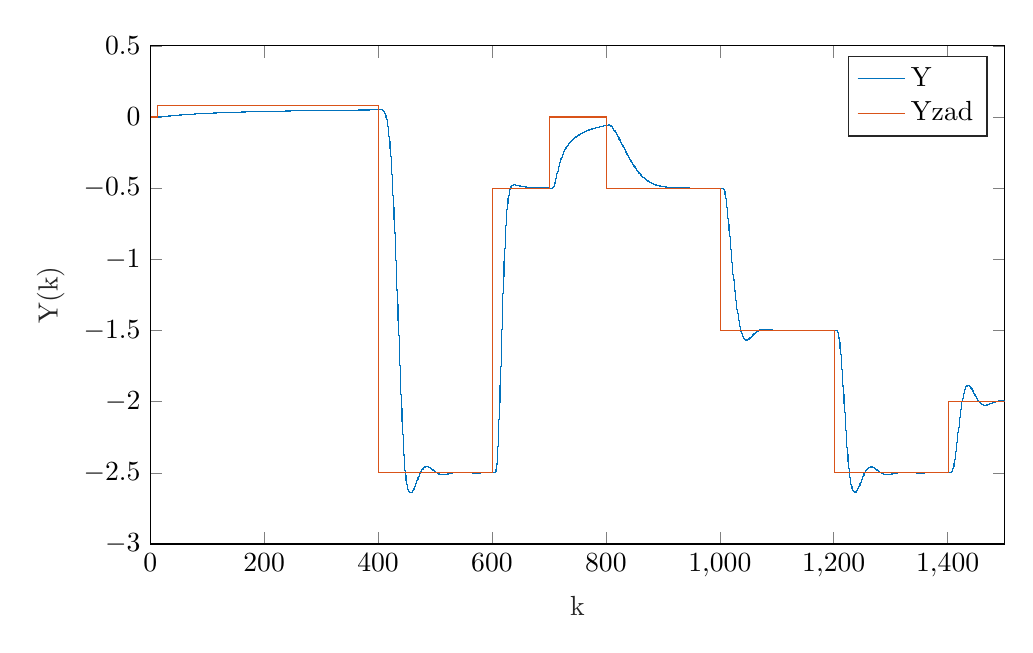
\begin{tikzpicture}

\begin{axis}[%
width=4.272in,
height=2.491in,
at={(0.717in,0.423in)},
scale only axis,
xmin=0,
xmax=1500,
xlabel style={font=\color{white!15!black}},
xlabel={k},
ymin=-3,
ymax=0.5,
ylabel style={font=\color{white!15!black}},
ylabel={Y(k)},
axis background/.style={fill=white},
legend style={legend cell align=left, align=left, draw=white!15!black}
]
\addplot[const plot, color=mycolor1] table[row sep=crcr] {%
1	0\\
2	0\\
3	0\\
4	0\\
5	0\\
6	0\\
7	0\\
8	0\\
9	0\\
10	0\\
11	0\\
12	0\\
13	0\\
14	0\\
15	0\\
16	0\\
17	6.49716531403557e-05\\
18	0.00025393973923361\\
19	0.000558961984996504\\
20	0.000948586707670891\\
21	0.00138989281339038\\
22	0.00185716775309152\\
23	0.00233342815699269\\
24	0.00280889155699224\\
25	0.00327870667684832\\
26	0.00374096367875215\\
27	0.00419528249671057\\
28	0.0046419456278738\\
29	0.0050814320866625\\
30	0.00551420512567238\\
31	0.00594064051854358\\
32	0.00636102161022591\\
33	0.00677555903164726\\
34	0.00718441435786914\\
35	0.00758771948813937\\
36	0.0079855898691351\\
37	0.00837813239500399\\
38	0.00876544956437675\\
39	0.00914764135188384\\
40	0.00952480585492487\\
41	0.00989703938041035\\
42	0.0102644363368567\\
43	0.0106270891044728\\
44	0.0109850879471681\\
45	0.0113385209773679\\
46	0.0116874741636808\\
47	0.0120320313668217\\
48	0.0123722743912488\\
49	0.0127082830438109\\
50	0.0130401351941895\\
51	0.013367906834429\\
52	0.0136916721363893\\
53	0.0140115035067892\\
54	0.0143274716398914\\
55	0.0146396455680128\\
56	0.0149480927100604\\
57	0.0152528789182628\\
58	0.0155540685232322\\
59	0.015851724377458\\
60	0.0161459078973139\\
61	0.0164366791036437\\
62	0.0167240966609845\\
63	0.0170082179154803\\
64	0.0172890989315358\\
65	0.0175667945272581\\
66	0.0178413583087326\\
67	0.0181128427031763\\
68	0.018381298991012\\
69	0.018646777336903\\
70	0.0189093268197876\\
71	0.0191689954619514\\
72	0.0194258302571723\\
73	0.0196798771979724\\
74	0.0199311813020109\\
75	0.020179786637648\\
76	0.0204257363487102\\
77	0.0206690726784875\\
78	0.020909836992987\\
79	0.0211480698034732\\
80	0.0213838107883178\\
81	0.0216170988141841\\
82	0.0218479719565706\\
83	0.0220764675197345\\
84	0.0223026220560183\\
85	0.0225264713845992\\
86	0.0227480506096825\\
87	0.022967394138156\\
88	0.0231845356967267\\
89	0.0233995083485548\\
90	0.0236123445094039\\
91	0.0238230759633225\\
92	0.0240317338778738\\
93	0.0242383488189276\\
94	0.0244429507650296\\
95	0.0246455691213623\\
96	0.0248462327333101\\
97	0.0250449698996426\\
98	0.0252418083853281\\
99	0.0254367754339889\\
100	0.0256298977800106\\
101	0.025821201660317\\
102	0.0260107128258196\\
103	0.0261984565525542\\
104	0.0263844576525126\\
105	0.0265687404841811\\
106	0.0267513289627927\\
107	0.0269322465703042\\
108	0.0271115163651051\\
109	0.0272891609914677\\
110	0.0274652026887459\\
111	0.0276396633003309\\
112	0.0278125642823701\\
113	0.0279839267122582\\
114	0.0281537712969058\\
115	0.0283221183807936\\
116	0.0284889879538174\\
117	0.0286543996589311\\
118	0.0288183727995931\\
119	0.0289809263470229\\
120	0.0291420789472722\\
121	0.0293018489281172\\
122	0.0294602543057765\\
123	0.0296173127914604\\
124	0.0297730417977555\\
125	0.0299274584448509\\
126	0.0300805795666091\\
127	0.0302324217164872\\
128	0.0303830011733114\\
129	0.0305323339469107\\
130	0.0306804357836123\\
131	0.0308273221716035\\
132	0.0309730083461633\\
133	0.0311175092947681\\
134	0.031260839762074\\
135	0.0314030142547801\\
136	0.0315440470463756\\
137	0.0316839521817743\\
138	0.0318227434818387\\
139	0.0319604345477981\\
140	0.0320970387655622\\
141	0.0322325693099346\\
142	0.0323670391487268\\
143	0.0325004610467781\\
144	0.032632847569881\\
145	0.0327642110886172\\
146	0.032894563782105\\
147	0.0330239176416611\\
148	0.0331522844743786\\
149	0.0332796759066244\\
150	0.0334061033874567\\
151	0.0335315781919661\\
152	0.0336561114245411\\
153	0.033779714022061\\
154	0.0339023967570176\\
155	0.0340241702405667\\
156	0.0341450449255135\\
157	0.034265031109231\\
158	0.0343841389365145\\
159	0.0345023784023741\\
160	0.0346197593547657\\
161	0.034736291497263\\
162	0.0348519843916713\\
163	0.0349668474605852\\
164	0.0350808899898911\\
165	0.0351941211312162\\
166	0.0353065499043248\\
167	0.0354181851994643\\
168	0.0355290357796607\\
169	0.0356391102829661\\
170	0.0357484172246588\\
171	0.0358569649993967\\
172	0.0359647618833264\\
173	0.0360718160361479\\
174	0.0361781355031367\\
175	0.0362837282171232\\
176	0.0363886020004325\\
177	0.0364927645667836\\
178	0.0365962235231494\\
179	0.0366989863715795\\
180	0.0368010605109852\\
181	0.0369024532388885\\
182	0.037003171753136\\
183	0.0371032231535779\\
184	0.0372026144437132\\
185	0.0373013525323025\\
186	0.0373994442349479\\
187	0.0374968962756421\\
188	0.0375937152882863\\
189	0.0376899078181785\\
190	0.0377854803234721\\
191	0.037880439176606\\
192	0.0379747906657072\\
193	0.0380685409959649\\
194	0.0381616962909791\\
195	0.0382542625940822\\
196	0.0383462458696357\\
197	0.038437652004301\\
198	0.0385284868082872\\
199	0.0386187560165735\\
200	0.0387084652901093\\
201	0.038797620216991\\
202	0.0388862263136169\\
203	0.0389742890258198\\
204	0.0390618137299781\\
205	0.0391488057341072\\
206	0.0392352702789288\\
207	0.0393212125389215\\
208	0.0394066376233515\\
209	0.0394915505772835\\
210	0.0395759563825742\\
211	0.0396598599588463\\
212	0.039743266164445\\
213	0.0398261797973772\\
214	0.0399086055962332\\
215	0.0399905482410918\\
216	0.0400720123544088\\
217	0.0401530025018896\\
218	0.0402335231933456\\
219	0.0403135788835359\\
220	0.0403931739729933\\
221	0.0404723128088355\\
222	0.0405509996855625\\
223	0.0406292388458388\\
224	0.0407070344812623\\
225	0.0407843907331201\\
226	0.0408613116931296\\
227	0.0409378014041678\\
228	0.0410138638609874\\
229	0.0410895030109201\\
230	0.041164722754568\\
231	0.0412395269464828\\
232	0.0413139193958336\\
233	0.041387903867062\\
234	0.0414614840805276\\
235	0.041534663713141\\
236	0.0416074463989868\\
237	0.0416798357299353\\
238	0.0417518352562443\\
239	0.0418234484871502\\
240	0.0418946788914498\\
241	0.0419655298980714\\
242	0.0420360048966369\\
243	0.0421061072380138\\
244	0.042175840234859\\
245	0.0422452071621525\\
246	0.0423142112577224\\
247	0.0423828557227617\\
248	0.0424511437223361\\
249	0.0425190783858832\\
250	0.0425866628077041\\
251	0.0426539000474463\\
252	0.0427207931305789\\
253	0.0427873450488605\\
254	0.0428535587607983\\
255	0.042919437192101\\
256	0.0429849832361238\\
257	0.0430501997543057\\
258	0.0431150895766008\\
259	0.0431796555019018\\
260	0.043243900298457\\
261	0.043307826704281\\
262	0.0433714374275576\\
263	0.043434735147038\\
264	0.0434977225124316\\
265	0.0435604021447904\\
266	0.0436227766368882\\
267	0.0436848485535932\\
268	0.043746620432235\\
269	0.0438080947829656\\
270	0.0438692740891149\\
271	0.0439301608075408\\
272	0.0439907573689738\\
273	0.0440510661783557\\
274	0.0441110896151741\\
275	0.0441708300337907\\
276	0.0442302897637653\\
277	0.0442894711101744\\
278	0.044348376353925\\
279	0.0444070077520635\\
280	0.0444653675380804\\
281	0.0445234579222098\\
282	0.0445812810917244\\
283	0.0446388392112264\\
284	0.0446961344229338\\
285	0.0447531688469622\\
286	0.0448099445816026\\
287	0.0448664637035952\\
288	0.0449227282683987\\
289	0.0449787403104558\\
290	0.0450345018434547\\
291	0.045090014860587\\
292	0.0451452813348011\\
293	0.0452003032190527\\
294	0.0452550824465511\\
295	0.0453096209310018\\
296	0.0453639205668459\\
297	0.0454179832294959\\
298	0.0454718107755678\\
299	0.0455254050431102\\
300	0.0455787678518297\\
301	0.0456319010033135\\
302	0.0456848062812482\\
303	0.0457374854516359\\
304	0.0457899402630072\\
305	0.0458421724466308\\
306	0.0458941837167202\\
307	0.0459459757706379\\
308	0.045997550289096\\
309	0.0460489089363547\\
310	0.046100053360417\\
311	0.0461509851932216\\
312	0.0462017060508328\\
313	0.0462522175336274\\
314	0.0463025212264791\\
315	0.0463526186989409\\
316	0.046402511505424\\
317	0.0464522011853748\\
318	0.0465016892634495\\
319	0.0465509772496858\\
320	0.046600066639673\\
321	0.0466489589147185\\
322	0.0466976555420136\\
323	0.0467461579747956\\
324	0.0467944676525085\\
325	0.0468425860009613\\
326	0.046890514432484\\
327	0.0469382543460816\\
328	0.0469858071275862\\
329	0.0470331741498064\\
330	0.0470803567726754\\
331	0.0471273563433967\\
332	0.0471741741965882\\
333	0.0472208116544235\\
334	0.0472672700267725\\
335	0.0473135506113392\\
336	0.0473596546937983\\
337	0.047405583547929\\
338	0.0474513384357485\\
339	0.0474969206076424\\
340	0.047542331302494\\
341	0.0475875717478117\\
342	0.047632643159855\\
343	0.0476775467437585\\
344	0.0477222836936545\\
345	0.0477668551927938\\
346	0.047811262413665\\
347	0.0478555065181124\\
348	0.0478995886574523\\
349	0.0479435099725875\\
350	0.0479872715941208\\
351	0.0480308746424665\\
352	0.0480743202279611\\
353	0.0481176094509719\\
354	0.0481607434020047\\
355	0.0482037231618099\\
356	0.0482465498014872\\
357	0.0482892243825893\\
358	0.0483317479572238\\
359	0.0483741215681541\\
360	0.0484163462488989\\
361	0.0484584230238308\\
362	0.048500352908273\\
363	0.0485421369085952\\
364	0.0485837760223084\\
365	0.0486252712381583\\
366	0.0486666235362173\\
367	0.0487078338879761\\
368	0.0487489032564333\\
369	0.0487898325961844\\
370	0.0488306228535096\\
371	0.0488712749664603\\
372	0.0489117898649452\\
373	0.0489521684708141\\
374	0.0489924116979419\\
375	0.0490325204523112\\
376	0.0490724956320932\\
377	0.0491123381277287\\
378	0.0491520488220075\\
379	0.0491916285901468\\
380	0.0492310782998686\\
381	0.0492703988114767\\
382	0.0493095909779322\\
383	0.0493486556449283\\
384	0.0493875936509642\\
385	0.0494264058274181\\
386	0.0494650929986191\\
387	0.0495036559819189\\
388	0.0495420955877617\\
389	0.0495804126197542\\
390	0.0496186078747339\\
391	0.0496566821428374\\
392	0.0496946362075672\\
393	0.0497324708458583\\
394	0.0497701868281432\\
395	0.0498077849184174\\
396	0.0498452658743028\\
397	0.0498826304471111\\
398	0.0499198793819064\\
399	0.0499570134175667\\
400	0.0499940332868454\\
401	0.0500309397164312\\
402	0.0500677334270078\\
403	0.0501044151333129\\
404	0.0501409855441966\\
405	0.0501774453626787\\
406	0.0501732789571122\\
407	0.0490041181697173\\
408	0.0465289453980899\\
409	0.0427578899345104\\
410	0.0376105023068085\\
411	0.0308706639244931\\
412	0.0221990320640032\\
413	0.0111600792543305\\
414	-0.00274895340394384\\
415	-0.0200693266291667\\
416	-0.0413521416210569\\
417	-0.0671300346350806\\
418	-0.0978903937090802\\
419	-0.134051766240842\\
420	-0.175945076767297\\
421	-0.223800774596798\\
422	-0.277742288381692\\
423	-0.337785409921024\\
424	-0.403842619616156\\
425	-0.475731006874428\\
426	-0.553182349411574\\
427	-0.635854050387701\\
428	-0.723339915402103\\
429	-0.815180098811299\\
430	-0.910869888912577\\
431	-1.00986728491841\\
432	-1.11159952037766\\
433	-1.21546880352156\\
434	-1.32085758500994\\
435	-1.42713364550781\\
436	-1.53365523944598\\
437	-1.63977645573738\\
438	-1.74485287613695\\
439	-1.84824753812405\\
440	-1.94933714834502\\
441	-2.04751844800545\\
442	-2.14147267608441\\
443	-2.22848358810272\\
444	-2.30650328920915\\
445	-2.37465324594974\\
446	-2.43286425401234\\
447	-2.48159968159205\\
448	-2.52164730965365\\
449	-2.55396666380376\\
450	-2.57958043162297\\
451	-2.59950025366284\\
452	-2.61467878083565\\
453	-2.62590782387723\\
454	-2.63378056968169\\
455	-2.63874159371501\\
456	-2.64114054645906\\
457	-2.64126819379351\\
458	-2.63937959601043\\
459	-2.63570844830602\\
460	-2.63047555223055\\
461	-2.6238934412912\\
462	-2.61616851420912\\
463	-2.60750158233319\\
464	-2.5980874412942\\
465	-2.58811388013876\\
466	-2.57776040947462\\
467	-2.56719690095978\\
468	-2.55658226907259\\
469	-2.54606328299561\\
470	-2.53577356549865\\
471	-2.52583281297533\\
472	-2.51634625375349\\
473	-2.50740434886004\\
474	-2.49908272955203\\
475	-2.49144235846869\\
476	-2.48452989577135\\
477	-2.47837824780542\\
478	-2.47300727339431\\
479	-2.46842462164989\\
480	-2.46462667496473\\
481	-2.46159957145728\\
482	-2.45932028239732\\
483	-2.45775772188354\\
484	-2.4568738681276\\
485	-2.45662487798627\\
486	-2.4569621787607\\
487	-2.4578335236554\\
488	-2.45918399958515\\
489	-2.46095697818128\\
490	-2.4630950028436\\
491	-2.46554060648905\\
492	-2.46823705625528\\
493	-2.4711290228281\\
494	-2.47416317328632\\
495	-2.47728868740934\\
496	-2.48045769828976\\
497	-2.48362565885352\\
498	-2.48675163653178\\
499	-2.48979853886883\\
500	-2.49273327330437\\
501	-2.49552684474878\\
502	-2.49815439488754\\
503	-2.50059518741376\\
504	-2.50283254360179\\
505	-2.50485373280417\\
506	-2.50664982258125\\
507	-2.50821549325898\\
508	-2.50954882175568\\
509	-2.51065103952311\\
510	-2.51152626941091\\
511	-2.51218124618475\\
512	-2.51262502530962\\
513	-2.51286868444874\\
514	-2.51292502192892\\
515	-2.51280825618522\\
516	-2.51253372992549\\
517	-2.51211762245162\\
518	-2.51157667324353\\
519	-2.51092791955935\\
520	-2.51018845043583\\
521	-2.509375179093\\
522	-2.50850463536206\\
523	-2.50759277937154\\
524	-2.50665483734988\\
525	-2.50570516003838\\
526	-2.504757103861\\
527	-2.50382293467352\\
528	-2.50291375361472\\
529	-2.50203944431333\\
530	-2.50120864046536\\
531	-2.50042871259121\\
532	-2.49970577261064\\
533	-2.49904469473534\\
534	-2.49844915107529\\
535	-2.49792166028229\\
536	-2.4974636475132\\
537	-2.49707551398197\\
538	-2.49675671438302\\
539	-2.49650584050511\\
540	-2.49632070941216\\
541	-2.4961984546429\\
542	-2.49613561897147\\
543	-2.49612824737364\\
544	-2.49617197895533\\
545	-2.49626213671937\\
546	-2.4963938141699\\
547	-2.49656195788013\\
548	-2.49676144527575\\
549	-2.4969871570116\\
550	-2.49723404344174\\
551	-2.49749718480167\\
552	-2.4977718448339\\
553	-2.49805351769586\\
554	-2.49833796808784\\
555	-2.49862126463183\\
556	-2.49889980661544\\
557	-2.49917034429124\\
558	-2.49942999298853\\
559	-2.4996762413532\\
560	-2.49990695408073\\
561	-2.50012036954865\\
562	-2.50031509278737\\
563	-2.50049008425298\\
564	-2.50064464488236\\
565	-2.50077839792062\\
566	-2.50089126801318\\
567	-2.50098345805123\\
568	-2.50105542424945\\
569	-2.50110784991968\\
570	-2.50114161838487\\
571	-2.50115778545316\\
572	-2.50115755184497\\
573	-2.50114223593532\\
574	-2.50111324714109\\
575	-2.50107206024844\\
576	-2.50102019093999\\
577	-2.50095917274549\\
578	-2.50089053560305\\
579	-2.50081578618242\\
580	-2.50073639008679\\
581	-2.50065375601549\\
582	-2.50056922193802\\
583	-2.50048404329947\\
584	-2.50039938324887\\
585	-2.50031630485656\\
586	-2.50023576526301\\
587	-2.50015861168084\\
588	-2.5000855791539\\
589	-2.50001728996154\\
590	-2.49995425454414\\
591	-2.4998968738153\\
592	-2.49984544271939\\
593	-2.49980015488759\\
594	-2.49976110824342\\
595	-2.49972831140799\\
596	-2.49970169075704\\
597	-2.49968109798497\\
598	-2.4996663180364\\
599	-2.49965707727182\\
600	-2.49965305174209\\
601	-2.49965387545482\\
602	-2.49965914852526\\
603	-2.49966844511486\\
604	-2.49968132107065\\
605	-2.49969732118998\\
606	-2.49315941679963\\
607	-2.47381474935816\\
608	-2.43813895711474\\
609	-2.38466928899471\\
610	-2.3134626693169\\
611	-2.22568044213178\\
612	-2.12328252967931\\
613	-2.00879707071039\\
614	-1.88513491477702\\
615	-1.75542777601278\\
616	-1.62287772286423\\
617	-1.49061300519765\\
618	-1.36155118615754\\
619	-1.2382751586021\\
620	-1.12293049086898\\
621	-1.01715311828546\\
622	-0.922034412978743\\
623	-0.83812648124052\\
624	-0.765485230707684\\
625	-0.703743728881004\\
626	-0.652204932887622\\
627	-0.609941716080927\\
628	-0.575893207315282\\
629	-0.548949151436768\\
630	-0.528017387845751\\
631	-0.512072792777888\\
632	-0.500188585946663\\
633	-0.491552540227098\\
634	-0.485471396530517\\
635	-0.481366870019993\\
636	-0.478766280944628\\
637	-0.477290273100951\\
638	-0.476639458539139\\
639	-0.476581250502284\\
640	-0.476937668293586\\
641	-0.477574532395752\\
642	-0.478392208837565\\
643	-0.479317891300825\\
644	-0.480299307572568\\
645	-0.481299684616319\\
646	-0.482293787774495\\
647	-0.483264852024444\\
648	-0.48420223775689\\
649	-0.485099663999796\\
650	-0.485953894321345\\
651	-0.486763772354134\\
652	-0.487529523640009\\
653	-0.488252257688995\\
654	-0.48893361862687\\
655	-0.489575544695589\\
656	-0.490180106431883\\
657	-0.490749400903612\\
658	-0.491285485260072\\
659	-0.491790337360283\\
660	-0.492265834655733\\
661	-0.492713745055027\\
662	-0.493135725380948\\
663	-0.493533324403063\\
664	-0.493907988416223\\
665	-0.494261068035294\\
666	-0.494593825364931\\
667	-0.494907441037925\\
668	-0.495203020840066\\
669	-0.495481601785808\\
670	-0.495744157601214\\
671	-0.495991603625627\\
672	-0.496224801173849\\
673	-0.496444561414822\\
674	-0.496651648826975\\
675	-0.496846784288632\\
676	-0.497030647856914\\
677	-0.497203881282122\\
678	-0.497367090297808\\
679	-0.497520846720223\\
680	-0.497665690384968\\
681	-0.497802130943527\\
682	-0.497930649538048\\
683	-0.498051700369187\\
684	-0.498165712168885\\
685	-0.498273089587698\\
686	-0.498374214504415\\
687	-0.498469447264331\\
688	-0.498559127851415\\
689	-0.498643576998778\\
690	-0.498723097241222\\
691	-0.498797973913144\\
692	-0.498868476094723\\
693	-0.498934857509009\\
694	-0.498997357372358\\
695	-0.499056201200435\\
696	-0.499111601571931\\
697	-0.49916375885197\\
698	-0.499212861877149\\
699	-0.49925908860401\\
700	-0.499302606722723\\
701	-0.49934357423765\\
702	-0.499382140016423\\
703	-0.499418444309082\\
704	-0.499452619238778\\
705	-0.499484789265473\\
706	-0.498031388475947\\
707	-0.493916186972984\\
708	-0.486751581708998\\
709	-0.476661359229039\\
710	-0.464063415888043\\
711	-0.449513264217081\\
712	-0.43359990326614\\
713	-0.416881107074372\\
714	-0.399846650948903\\
715	-0.382900841895328\\
716	-0.366358103520327\\
717	-0.35044707374407\\
718	-0.335319871773648\\
719	-0.32106406178982\\
720	-0.307715510604596\\
721	-0.29527087586688\\
722	-0.283698904138075\\
723	-0.272950075241718\\
724	-0.262964409878\\
725	-0.253677462839831\\
726	-0.245024661215851\\
727	-0.236944225857138\\
728	-0.229378946775925\\
729	-0.222277081370971\\
730	-0.215592620077894\\
731	-0.209285127199974\\
732	-0.203319323090684\\
733	-0.197664533073834\\
734	-0.192294091980127\\
735	-0.187184762738962\\
736	-0.182316203619772\\
737	-0.177670501150337\\
738	-0.173231773638604\\
739	-0.168985842557958\\
740	-0.164919964762917\\
741	-0.161022616614292\\
742	-0.157283320795831\\
743	-0.153692507260483\\
744	-0.150241400885831\\
745	-0.146921929725575\\
746	-0.14372664901719\\
747	-0.140648677235275\\
748	-0.13768164141847\\
749	-0.134819629739142\\
750	-0.132057149846386\\
751	-0.129389091922813\\
752	-0.126810695685519\\
753	-0.124317520761267\\
754	-0.121905420000575\\
755	-0.119570515385359\\
756	-0.117309176245145\\
757	-0.115117999538503\\
758	-0.112993791986606\\
759	-0.110933553869193\\
760	-0.108934464312789\\
761	-0.106993867918084\\
762	-0.105109262588899\\
763	-0.103278288439412\\
764	-0.10149871766941\\
765	-0.0997684453093204\\
766	-0.0980854807476401\\
767	-0.0964479399631274\\
768	-0.0948540383928335\\
769	-0.093302084374742\\
770	-0.0917904731105733\\
771	-0.0903176811002715\\
772	-0.0888822610049238\\
773	-0.0874828368994526\\
774	-0.0861180998804536\\
775	-0.0847868039981037\\
776	-0.0834877624841918\\
777	-0.0822198442510989\\
778	-0.0809819706390046\\
779	-0.0797731123907856\\
780	-0.0785922868360105\\
781	-0.077438555267178\\
782	-0.0763110204928931\\
783	-0.0752088245540719\\
784	-0.0741311465905144\\
785	-0.0730772008463056\\
786	-0.0720462348035209\\
787	-0.0710375274346192\\
788	-0.0700503875647324\\
789	-0.0690841523358037\\
790	-0.0681381857651986\\
791	-0.0672118773920245\\
792	-0.0663046410049447\\
793	-0.0654159134457793\\
794	-0.0645451534836367\\
795	-0.06369184075474\\
796	-0.0628554747634882\\
797	-0.0620355739406371\\
798	-0.0612316747548027\\
799	-0.0604433308737765\\
800	-0.0596701123724033\\
801	-0.0589116049840188\\
802	-0.0581674093926605\\
803	-0.0574371405634709\\
804	-0.0567204271088972\\
805	-0.0560169106884648\\
806	-0.0560515015787161\\
807	-0.0573848078664677\\
808	-0.060049036596497\\
809	-0.0638452768405366\\
810	-0.0685135416499963\\
811	-0.0738158888868983\\
812	-0.0795664820665539\\
813	-0.085633927367204\\
814	-0.0919320084425149\\
815	-0.0984075384122665\\
816	-0.105029323832602\\
817	-0.111779604554343\\
818	-0.118648048119485\\
819	-0.12562786193794\\
820	-0.132713465961962\\
821	-0.139899223170817\\
822	-0.147178837264714\\
823	-0.15454514250974\\
824	-0.161990104702681\\
825	-0.169504921875167\\
826	-0.177080161221504\\
827	-0.184705899240711\\
828	-0.192371850287059\\
829	-0.20006747878769\\
830	-0.207782095392593\\
831	-0.215504939386745\\
832	-0.223225250180284\\
833	-0.230932330428149\\
834	-0.238615602785763\\
835	-0.246264661727195\\
836	-0.253869321347985\\
837	-0.261419659683457\\
838	-0.268906059794373\\
839	-0.276319247688702\\
840	-0.283650327039734\\
841	-0.290890810606779\\
842	-0.298032648248367\\
843	-0.305068251426158\\
844	-0.311990514121279\\
845	-0.318792830116674\\
846	-0.325469106634843\\
847	-0.332013774357045\\
848	-0.338421793885638\\
849	-0.344688658744748\\
850	-0.350810395044936\\
851	-0.356783557964803\\
852	-0.362605225226175\\
853	-0.368272987759653\\
854	-0.373784937773854\\
855	-0.379139654454714\\
856	-0.384336187530803\\
857	-0.38937403894696\\
858	-0.394253142891713\\
859	-0.398973844424234\\
860	-0.403536876944082\\
861	-0.407943338742032\\
862	-0.412194668863021\\
863	-0.416292622503002\\
864	-0.420239246150477\\
865	-0.424036852671016\\
866	-0.427687996519336\\
867	-0.431195449248861\\
868	-0.434562175473338\\
869	-0.437791309419252\\
870	-0.440886132191761\\
871	-0.443850049860843\\
872	-0.446686572458512\\
873	-0.449399293962496\\
874	-0.451991873326867\\
875	-0.454468016605844\\
876	-0.456831460203567\\
877	-0.459085955270032\\
878	-0.461235253251796\\
879	-0.463283092595401\\
880	-0.465233186591951\\
881	-0.467089212342692\\
882	-0.468854800818024\\
883	-0.470533527975892\\
884	-0.472128906900084\\
885	-0.473644380914481\\
886	-0.475083317625737\\
887	-0.476449003844135\\
888	-0.477744641330474\\
889	-0.478973343315603\\
890	-0.480138131738709\\
891	-0.481241935150475\\
892	-0.482287587227813\\
893	-0.483277825847852\\
894	-0.484215292670274\\
895	-0.485102533178789\\
896	-0.485941997134512\\
897	-0.486736039396181\\
898	-0.487486921064499\\
899	-0.488196810910307\\
900	-0.488867787048833\\
901	-0.489501838824788\\
902	-0.490100868875639\\
903	-0.490666695342902\\
904	-0.491201054203782\\
905	-0.491705601697859\\
906	-0.492181916825877\\
907	-0.492631503899863\\
908	-0.493055795125947\\
909	-0.493456153203233\\
910	-0.493833873923948\\
911	-0.494190188761851\\
912	-0.494526267437518\\
913	-0.494843220450629\\
914	-0.495142101570765\\
915	-0.495423910279523\\
916	-0.495689594157887\\
917	-0.495940051213895\\
918	-0.496176132146551\\
919	-0.496398642542833\\
920	-0.496608345005386\\
921	-0.496805961209205\\
922	-0.496992173886191\\
923	-0.497167628737029\\
924	-0.497332936270272\\
925	-0.497488673568957\\
926	-0.497635385985408\\
927	-0.497773588765184\\
928	-0.497903768601397\\
929	-0.498026385120819\\
930	-0.498141872303397\\
931	-0.498250639836908\\
932	-0.49835307440863\\
933	-0.498449540935964\\
934	-0.498540383738021\\
935	-0.498625927650227\\
936	-0.498706479084023\\
937	-0.498782327033744\\
938	-0.498853744032761\\
939	-0.498920987060951\\
940	-0.498984298405543\\
941	-0.499043906477333\\
942	-0.499100026584256\\
943	-0.499152861664216\\
944	-0.499202602979067\\
945	-0.499249430771543\\
946	-0.499293514886908\\
947	-0.49933501536104\\
948	-0.49937408297656\\
949	-0.499410859788633\\
950	-0.499445479621918\\
951	-0.499478068540168\\
952	-0.499508745289846\\
953	-0.499537621719132\\
954	-0.499564803173576\\
955	-0.499590388869639\\
956	-0.499614472247291\\
957	-0.499637141302775\\
958	-0.499658478902608\\
959	-0.499678563079829\\
960	-0.49969746731345\\
961	-0.499715260792038\\
962	-0.499732008662289\\
963	-0.499747772263422\\
964	-0.499762609348174\\
965	-0.499776574291149\\
966	-0.499789718285207\\
967	-0.499802089526587\\
968	-0.499813733389364\\
969	-0.499824692589875\\
970	-0.499835007341642\\
971	-0.499844715501365\\
972	-0.499853852706466\\
973	-0.499862452504669\\
974	-0.499870546476085\\
975	-0.499878164348202\\
976	-0.499885334104215\\
977	-0.49989208208505\\
978	-0.499898433085466\\
979	-0.499904410444563\\
980	-0.499910036131016\\
981	-0.499915330823352\\
982	-0.49992031398554\\
983	-0.499925003938172\\
984	-0.499929417925498\\
985	-0.499933572178535\\
986	-0.499937481974497\\
987	-0.49994116169275\\
988	-0.499944624867496\\
989	-0.499947884237371\\
990	-0.499950951792146\\
991	-0.499953838816691\\
992	-0.499956555932367\\
993	-0.499959113135991\\
994	-0.499961519836517\\
995	-0.499963784889575\\
996	-0.499965916629972\\
997	-0.4999679229023\\
998	-0.499969811089742\\
999	-0.499971588141187\\
1000	-0.49997326059676\\
1001	-0.499974834611845\\
1002	-0.499976315979709\\
1003	-0.499977710152788\\
1004	-0.499979022262727\\
1005	-0.499980257139241\\
1006	-0.502888294260853\\
1007	-0.510992584626134\\
1008	-0.525124309749285\\
1009	-0.545238919592087\\
1010	-0.570822313281841\\
1011	-0.601151230310568\\
1012	-0.635445346871535\\
1013	-0.672948011760356\\
1014	-0.712963646609208\\
1015	-0.754870497067698\\
1016	-0.798120401962986\\
1017	-0.842232521300376\\
1018	-0.886784948820633\\
1019	-0.931406283751957\\
1020	-0.975768140802819\\
1021	-1.01957895645857\\
1022	-1.06257911706279\\
1023	-1.10453727641752\\
1024	-1.14524766545739\\
1025	-1.1845281846985\\
1026	-1.22221908495319\\
1027	-1.25818206721267\\
1028	-1.29229966066662\\
1029	-1.32447476461179\\
1030	-1.35463026383799\\
1031	-1.38270864752752\\
1032	-1.40867157891747\\
1033	-1.43249937735815\\
1034	-1.45419038642313\\
1035	-1.47376021182065\\
1036	-1.49124082139064\\
1037	-1.50667950672685\\
1038	-1.52013771214734\\
1039	-1.53168974198621\\
1040	-1.54142136157932\\
1041	-1.54942831091234\\
1042	-1.55581475270704\\
1043	-1.56069167874482\\
1044	-1.56417529946309\\
1045	-1.56638544231364\\
1046	-1.5674439840583\\
1047	-1.56747334112825\\
1048	-1.56659504044403\\
1049	-1.56492839075747\\
1050	-1.56258927173224\\
1051	-1.55968905473772\\
1052	-1.55633366582006\\
1053	-1.55262279766635\\
1054	-1.54864927372716\\
1055	-1.54449856413762\\
1056	-1.54024844979207\\
1057	-1.53596882798089\\
1058	-1.53172165046664\\
1059	-1.52756098281269\\
1060	-1.52353317220949\\
1061	-1.51967710997649\\
1062	-1.51602457433356\\
1063	-1.51260063890115\\
1064	-1.50942413265252\\
1065	-1.5065081376461\\
1066	-1.50386051174588\\
1067	-1.50148442462694\\
1068	-1.4993788965959\\
1069	-1.49753933107382\\
1070	-1.49595803293682\\
1071	-1.49462470624273\\
1072	-1.49352692615413\\
1073	-1.4926505810689\\
1074	-1.49198028207136\\
1075	-1.49149973780518\\
1076	-1.49119209373894\\
1077	-1.49104023554414\\
1078	-1.49102705693816\\
1079	-1.49113569286634\\
1080	-1.49134971931727\\
1081	-1.49165332139264\\
1082	-1.49203143149921\\
1083	-1.4924698397042\\
1084	-1.49295527840888\\
1085	-1.49347548355624\\
1086	-1.4940192346066\\
1087	-1.49457637549799\\
1088	-1.49513781876187\\
1089	-1.49569553489619\\
1090	-1.49624252901121\\
1091	-1.49677280666346\\
1092	-1.49728133068292\\
1093	-1.49776397068171\\
1094	-1.49821744681013\\
1095	-1.49863926920196\\
1096	-1.49902767442509\\
1097	-1.49938156012873\\
1098	-1.499700418955\\
1099	-1.49998427266209\\
1100	-1.50023360728876\\
1101	-1.50044931007721\\
1102	-1.50063260876293\\
1103	-1.50078501373779\\
1104	-1.50090826349548\\
1105	-1.50100427367802\\
1106	-1.50107508995811\\
1107	-1.50112284491453\\
1108	-1.50114971898795\\
1109	-1.50115790554063\\
1110	-1.50114957998774\\
1111	-1.50112687291801\\
1112	-1.50109184707922\\
1113	-1.50104647806766\\
1114	-1.50099263853099\\
1115	-1.50093208566996\\
1116	-1.50086645180657\\
1117	-1.50079723777275\\
1118	-1.50072580886606\\
1119	-1.50065339311451\\
1120	-1.5005810815932\\
1121	-1.5005098305388\\
1122	-1.5004404650144\\
1123	-1.50037368388669\\
1124	-1.50031006588819\\
1125	-1.50025007655094\\
1126	-1.5001940758116\\
1127	-1.50014232610382\\
1128	-1.50009500076938\\
1129	-1.50005219263597\\
1130	-1.50001392262579\\
1131	-1.49998014827554\\
1132	-1.49995077206396\\
1133	-1.49992564945863\\
1134	-1.49990459660821\\
1135	-1.4998873976202\\
1136	-1.49987381137734\\
1137	-1.49986357785748\\
1138	-1.49985642393304\\
1139	-1.49985206863596\\
1140	-1.49985022788301\\
1141	-1.49985061866413\\
1142	-1.49985296270355\\
1143	-1.4998569896091\\
1144	-1.49986243953025\\
1145	-1.49986906534941\\
1146	-1.49987663443437\\
1147	-1.4998849299821\\
1148	-1.49989375198593\\
1149	-1.49990291785942\\
1150	-1.49991226275044\\
1151	-1.49992163957927\\
1152	-1.49993091883403\\
1153	-1.4999399881558\\
1154	-1.49994875174483\\
1155	-1.49995712961757\\
1156	-1.49996505674285\\
1157	-1.49997248208348\\
1158	-1.49997936756772\\
1159	-1.4999856870129\\
1160	-1.49999142502162\\
1161	-1.49999657586842\\
1162	-1.50000114239322\\
1163	-1.50000513491536\\
1164	-1.50000857018039\\
1165	-1.50001147034957\\
1166	-1.50001386204049\\
1167	-1.50001577542537\\
1168	-1.50001724339203\\
1169	-1.50001830077117\\
1170	-1.50001898363213\\
1171	-1.50001932864817\\
1172	-1.50001937253142\\
1173	-1.5000191515363\\
1174	-1.50001870102991\\
1175	-1.50001805512683\\
1176	-1.50001724638536\\
1177	-1.50001630556181\\
1178	-1.50001526141894\\
1179	-1.50001414058456\\
1180	-1.50001296745605\\
1181	-1.50001176414639\\
1182	-1.50001055046743\\
1183	-1.50000934394604\\
1184	-1.50000815986885\\
1185	-1.50000701135158\\
1186	-1.50000590942892\\
1187	-1.50000486316135\\
1188	-1.50000387975526\\
1189	-1.50000296469328\\
1190	-1.50000212187173\\
1191	-1.50000135374251\\
1192	-1.50000066145696\\
1193	-1.50000004500957\\
1194	-1.49999950337958\\
1195	-1.49999903466888\\
1196	-1.49999863623477\\
1197	-1.49999830481646\\
1198	-1.49999803665438\\
1199	-1.49999782760156\\
1200	-1.4999976732266\\
1201	-1.49999756890778\\
1202	-1.49999750991834\\
1203	-1.49999749150256\\
1204	-1.49999750894308\\
1205	-1.49999755761936\\
1206	-1.50318469703997\\
1207	-1.51233753005602\\
1208	-1.52880601876462\\
1209	-1.55297930668191\\
1210	-1.58463699952018\\
1211	-1.62319604719325\\
1212	-1.66787382792386\\
1213	-1.71779193139939\\
1214	-1.7720405532776\\
1215	-1.8297174540579\\
1216	-1.8899507909465\\
1217	-1.9519119232879\\
1218	-2.01482214854827\\
1219	-2.07795590406311\\
1220	-2.14064202756255\\
1221	-2.20226404676226\\
1222	-2.26226005890606\\
1223	-2.32012250015967\\
1224	-2.37433096826306\\
1225	-2.42344538799628\\
1226	-2.4667166736317\\
1227	-2.50395418318358\\
1228	-2.5353420661784\\
1229	-2.56130003723131\\
1230	-2.58238031388967\\
1231	-2.59919346782481\\
1232	-2.612340431935\\
1233	-2.62229707063966\\
1234	-2.62942260159238\\
1235	-2.63400255732269\\
1236	-2.63627830522462\\
1237	-2.63646619178279\\
1238	-2.63476929105646\\
1239	-2.63138418418975\\
1240	-2.62650446836601\\
1241	-2.62032213706254\\
1242	-2.61302759908676\\
1243	-2.60480885515653\\
1244	-2.59585018588692\\
1245	-2.5863305949761\\
1246	-2.57642217693561\\
1247	-2.56628852739558\\
1248	-2.55608327777772\\
1249	-2.54594880979743\\
1250	-2.53601518553821\\
1251	-2.52639931365649\\
1252	-2.51720436032804\\
1253	-2.5085194040379\\
1254	-2.50041932575456\\
1255	-2.49296492010798\\
1256	-2.48620320870502\\
1257	-2.4801679335097\\
1258	-2.47488020615467\\
1259	-2.47034928800202\\
1260	-2.46657347560024\\
1261	-2.46354106675002\\
1262	-2.4612313835517\\
1263	-2.45961583042318\\
1264	-2.45865896701533\\
1265	-2.45831957809406\\
1266	-2.45855172469679\\
1267	-2.4593057631199\\
1268	-2.46052932048068\\
1269	-2.46216821767109\\
1270	-2.46416733244352\\
1271	-2.46647139711929\\
1272	-2.46902572697888\\
1273	-2.47177687677766\\
1274	-2.47467322404071\\
1275	-2.47766547883535\\
1276	-2.48070712061684\\
1277	-2.48375476350694\\
1278	-2.48676845201358\\
1279	-2.48971188974837\\
1280	-2.49255260416148\\
1281	-2.49526205070232\\
1282	-2.49781566014026\\
1283	-2.50019283304974\\
1284	-2.50237688568435\\
1285	-2.5043549516401\\
1286	-2.50611784384006\\
1287	-2.50765988146408\\
1288	-2.50897868649768\\
1289	-2.51007495458441\\
1290	-2.51095220483544\\
1291	-2.51161651317898\\
1292	-2.5120762337206\\
1293	-2.51234171243408\\
1294	-2.51242499731283\\
1295	-2.51233954888554\\
1296	-2.51209995473998\\
1297	-2.51172165140837\\
1298	-2.51122065665168\\
1299	-2.51061331484198\\
1300	-2.50991605778809\\
1301	-2.50914518298452\\
1302	-2.50831665089373\\
1303	-2.5074459025022\\
1304	-2.50654769802722\\
1305	-2.50563597729984\\
1306	-2.50472374201329\\
1307	-2.50382295971172\\
1308	-2.50294448910348\\
1309	-2.50209802602014\\
1310	-2.50129206910928\\
1311	-2.50053390414736\\
1312	-2.49982960568943\\
1313	-2.49918405463534\\
1314	-2.4986009701873\\
1315	-2.49808295459939\\
1316	-2.49763154907544\\
1317	-2.4972472991547\\
1318	-2.49692982793327\\
1319	-2.49667791550077\\
1320	-2.49648958302343\\
1321	-2.4963621799741\\
1322	-2.49629247309402\\
1323	-2.49627673576731\\
1324	-2.49631083659545\\
1325	-2.49639032607195\\
1326	-2.49651052037543\\
1327	-2.49666658142025\\
1328	-2.49685359242506\\
1329	-2.49706662838074\\
1330	-2.49730082091694\\
1331	-2.49755141718128\\
1332	-2.49781383245472\\
1333	-2.49808369633043\\
1334	-2.4983568923806\\
1335	-2.49862959132564\\
1336	-2.4988982778023\\
1337	-2.49915977090175\\
1338	-2.49941123871419\\
1339	-2.49965020717432\\
1340	-2.49987456355132\\
1341	-2.50008255496764\\
1342	-2.50027278236395\\
1343	-2.50044419035251\\
1344	-2.50059605341858\\
1345	-2.50072795893992\\
1346	-2.50083978749789\\
1347	-2.50093169095097\\
1348	-2.50100406873305\\
1349	-2.50105754282525\\
1350	-2.50109293183157\\
1351	-2.50111122456636\\
1352	-2.50111355353572\\
1353	-2.50110116866625\\
1354	-2.50107541160305\\
1355	-2.50103769086671\\
1356	-2.50098945812435\\
1357	-2.50093218579541\\
1358	-2.50086734617794\\
1359	-2.50079639224658\\
1360	-2.50072074023952\\
1361	-2.50064175411913\\
1362	-2.50056073195955\\
1363	-2.50047889428532\\
1364	-2.50039737435718\\
1365	-2.50031721037649\\
1366	-2.50023933955649\\
1367	-2.50016459398827\\
1368	-2.50009369821185\\
1369	-2.50002726838716\\
1370	-2.49996581294757\\
1371	-2.49990973460817\\
1372	-2.49985933359401\\
1373	-2.49981481194774\\
1374	-2.49977627877382\\
1375	-2.49974375627534\\
1376	-2.49971718644077\\
1377	-2.49969643824105\\
1378	-2.49968131520186\\
1379	-2.49967156322194\\
1380	-2.49966687851565\\
1381	-2.49966691556592\\
1382	-2.49967129498295\\
1383	-2.49967961117367\\
1384	-2.49969143973702\\
1385	-2.49970634451071\\
1386	-2.49972388420532\\
1387	-2.49974361857262\\
1388	-2.4997651140649\\
1389	-2.49978794895251\\
1390	-2.49981171787636\\
1391	-2.49983603582145\\
1392	-2.4998605415061\\
1393	-2.49988490018964\\
1394	-2.49990880590863\\
1395	-2.49993198315835\\
1396	-2.49995418804218\\
1397	-2.49997520891659\\
1398	-2.49999486656374\\
1399	-2.5000130139275\\
1400	-2.5000295354511\\
1401	-2.50004434605731\\
1402	-2.50005738981283\\
1403	-2.5000686383198\\
1404	-2.50007808887723\\
1405	-2.50008576245473\\
1406	-2.49847822696244\\
1407	-2.49375015616343\\
1408	-2.48507963642413\\
1409	-2.4721390446992\\
1410	-2.45494532772036\\
1411	-2.43374832032699\\
1412	-2.40895137964827\\
1413	-2.38105540655201\\
1414	-2.35061861765136\\
1415	-2.31822679187542\\
1416	-2.28447062214524\\
1417	-2.24992809648043\\
1418	-2.215150655021\\
1419	-2.18065237177798\\
1420	-2.14690170426742\\
1421	-2.11431551542014\\
1422	-2.08325515032244\\
1423	-2.05402437572377\\
1424	-2.02686899024838\\
1425	-2.00197790002162\\
1426	-1.97948543870749\\
1427	-1.95947469983419\\
1428	-1.94198164626674\\
1429	-1.92699976798003\\
1430	-1.91448507441238\\
1431	-1.90436123004301\\
1432	-1.8965246692353\\
1433	-1.89084955644432\\
1434	-1.88719248837323\\
1435	-1.88539686371432\\
1436	-1.88529687234149\\
1437	-1.88672107835066\\
1438	-1.88949558975537\\
1439	-1.89344682190973\\
1440	-1.89840387210955\\
1441	-1.90420052976955\\
1442	-1.91067695064564\\
1443	-1.91768102535599\\
1444	-1.92506947251847\\
1445	-1.93270868567806\\
1446	-1.94047536127966\\
1447	-1.94825693260308\\
1448	-1.95595183208856\\
1449	-1.96346960204019\\
1450	-1.97073087143335\\
1451	-1.97766721455074\\
1452	-1.98422090546805\\
1453	-1.99034458101039\\
1454	-1.99600082368937\\
1455	-2.00116167527616\\
1456	-2.00580809102776\\
1457	-2.00992934411758\\
1458	-2.01352238948082\\
1459	-2.01659119602675\\
1460	-2.01914605595238\\
1461	-2.02120287968069\\
1462	-2.02278248471053\\
1463	-2.02390988638158\\
1464	-2.02461359820894\\
1465	-2.02492494901656\\
1466	-2.02487742359236\\
1467	-2.02450603300082\\
1468	-2.02384672002651\\
1469	-2.02293580449439\\
1470	-2.02180947243298\\
1471	-2.02050331223015\\
1472	-2.01905190009585\\
1473	-2.01748843630946\\
1474	-2.01584443290992\\
1475	-2.01414945270074\\
1476	-2.01243089870544\\
1477	-2.01071385253517\\
1478	-2.0090209595296\\
1479	-2.00737235801333\\
1480	-2.00578564957803\\
1481	-2.00427590695777\\
1482	-2.00285571581119\\
1483	-2.00153524655708\\
1484	-2.00032235232477\\
1485	-1.99922268907083\\
1486	-1.99823985397228\\
1487	-1.99737553832413\\
1488	-1.99662969133769\\
1489	-1.99600069144624\\
1490	-1.99548552196695\\
1491	-1.99507994823489\\
1492	-1.99477869360753\\
1493	-1.99457561202963\\
1494	-1.994463855143\\
1495	-1.9944360322165\\
1496	-1.99448436145568\\
1497	-1.99460081152368\\
1498	-1.99477723236366\\
1499	-1.99500547465415\\
1500	-1.99527749745329\\
};
\addlegendentry{Y}

\addplot[const plot, color=mycolor2] table[row sep=crcr] {%
1	0\\
2	0\\
3	0\\
4	0\\
5	0\\
6	0\\
7	0\\
8	0\\
9	0\\
10	0\\
11	0\\
12	0.08\\
13	0.08\\
14	0.08\\
15	0.08\\
16	0.08\\
17	0.08\\
18	0.08\\
19	0.08\\
20	0.08\\
21	0.08\\
22	0.08\\
23	0.08\\
24	0.08\\
25	0.08\\
26	0.08\\
27	0.08\\
28	0.08\\
29	0.08\\
30	0.08\\
31	0.08\\
32	0.08\\
33	0.08\\
34	0.08\\
35	0.08\\
36	0.08\\
37	0.08\\
38	0.08\\
39	0.08\\
40	0.08\\
41	0.08\\
42	0.08\\
43	0.08\\
44	0.08\\
45	0.08\\
46	0.08\\
47	0.08\\
48	0.08\\
49	0.08\\
50	0.08\\
51	0.08\\
52	0.08\\
53	0.08\\
54	0.08\\
55	0.08\\
56	0.08\\
57	0.08\\
58	0.08\\
59	0.08\\
60	0.08\\
61	0.08\\
62	0.08\\
63	0.08\\
64	0.08\\
65	0.08\\
66	0.08\\
67	0.08\\
68	0.08\\
69	0.08\\
70	0.08\\
71	0.08\\
72	0.08\\
73	0.08\\
74	0.08\\
75	0.08\\
76	0.08\\
77	0.08\\
78	0.08\\
79	0.08\\
80	0.08\\
81	0.08\\
82	0.08\\
83	0.08\\
84	0.08\\
85	0.08\\
86	0.08\\
87	0.08\\
88	0.08\\
89	0.08\\
90	0.08\\
91	0.08\\
92	0.08\\
93	0.08\\
94	0.08\\
95	0.08\\
96	0.08\\
97	0.08\\
98	0.08\\
99	0.08\\
100	0.08\\
101	0.08\\
102	0.08\\
103	0.08\\
104	0.08\\
105	0.08\\
106	0.08\\
107	0.08\\
108	0.08\\
109	0.08\\
110	0.08\\
111	0.08\\
112	0.08\\
113	0.08\\
114	0.08\\
115	0.08\\
116	0.08\\
117	0.08\\
118	0.08\\
119	0.08\\
120	0.08\\
121	0.08\\
122	0.08\\
123	0.08\\
124	0.08\\
125	0.08\\
126	0.08\\
127	0.08\\
128	0.08\\
129	0.08\\
130	0.08\\
131	0.08\\
132	0.08\\
133	0.08\\
134	0.08\\
135	0.08\\
136	0.08\\
137	0.08\\
138	0.08\\
139	0.08\\
140	0.08\\
141	0.08\\
142	0.08\\
143	0.08\\
144	0.08\\
145	0.08\\
146	0.08\\
147	0.08\\
148	0.08\\
149	0.08\\
150	0.08\\
151	0.08\\
152	0.08\\
153	0.08\\
154	0.08\\
155	0.08\\
156	0.08\\
157	0.08\\
158	0.08\\
159	0.08\\
160	0.08\\
161	0.08\\
162	0.08\\
163	0.08\\
164	0.08\\
165	0.08\\
166	0.08\\
167	0.08\\
168	0.08\\
169	0.08\\
170	0.08\\
171	0.08\\
172	0.08\\
173	0.08\\
174	0.08\\
175	0.08\\
176	0.08\\
177	0.08\\
178	0.08\\
179	0.08\\
180	0.08\\
181	0.08\\
182	0.08\\
183	0.08\\
184	0.08\\
185	0.08\\
186	0.08\\
187	0.08\\
188	0.08\\
189	0.08\\
190	0.08\\
191	0.08\\
192	0.08\\
193	0.08\\
194	0.08\\
195	0.08\\
196	0.08\\
197	0.08\\
198	0.08\\
199	0.08\\
200	0.08\\
201	0.08\\
202	0.08\\
203	0.08\\
204	0.08\\
205	0.08\\
206	0.08\\
207	0.08\\
208	0.08\\
209	0.08\\
210	0.08\\
211	0.08\\
212	0.08\\
213	0.08\\
214	0.08\\
215	0.08\\
216	0.08\\
217	0.08\\
218	0.08\\
219	0.08\\
220	0.08\\
221	0.08\\
222	0.08\\
223	0.08\\
224	0.08\\
225	0.08\\
226	0.08\\
227	0.08\\
228	0.08\\
229	0.08\\
230	0.08\\
231	0.08\\
232	0.08\\
233	0.08\\
234	0.08\\
235	0.08\\
236	0.08\\
237	0.08\\
238	0.08\\
239	0.08\\
240	0.08\\
241	0.08\\
242	0.08\\
243	0.08\\
244	0.08\\
245	0.08\\
246	0.08\\
247	0.08\\
248	0.08\\
249	0.08\\
250	0.08\\
251	0.08\\
252	0.08\\
253	0.08\\
254	0.08\\
255	0.08\\
256	0.08\\
257	0.08\\
258	0.08\\
259	0.08\\
260	0.08\\
261	0.08\\
262	0.08\\
263	0.08\\
264	0.08\\
265	0.08\\
266	0.08\\
267	0.08\\
268	0.08\\
269	0.08\\
270	0.08\\
271	0.08\\
272	0.08\\
273	0.08\\
274	0.08\\
275	0.08\\
276	0.08\\
277	0.08\\
278	0.08\\
279	0.08\\
280	0.08\\
281	0.08\\
282	0.08\\
283	0.08\\
284	0.08\\
285	0.08\\
286	0.08\\
287	0.08\\
288	0.08\\
289	0.08\\
290	0.08\\
291	0.08\\
292	0.08\\
293	0.08\\
294	0.08\\
295	0.08\\
296	0.08\\
297	0.08\\
298	0.08\\
299	0.08\\
300	0.08\\
301	0.08\\
302	0.08\\
303	0.08\\
304	0.08\\
305	0.08\\
306	0.08\\
307	0.08\\
308	0.08\\
309	0.08\\
310	0.08\\
311	0.08\\
312	0.08\\
313	0.08\\
314	0.08\\
315	0.08\\
316	0.08\\
317	0.08\\
318	0.08\\
319	0.08\\
320	0.08\\
321	0.08\\
322	0.08\\
323	0.08\\
324	0.08\\
325	0.08\\
326	0.08\\
327	0.08\\
328	0.08\\
329	0.08\\
330	0.08\\
331	0.08\\
332	0.08\\
333	0.08\\
334	0.08\\
335	0.08\\
336	0.08\\
337	0.08\\
338	0.08\\
339	0.08\\
340	0.08\\
341	0.08\\
342	0.08\\
343	0.08\\
344	0.08\\
345	0.08\\
346	0.08\\
347	0.08\\
348	0.08\\
349	0.08\\
350	0.08\\
351	0.08\\
352	0.08\\
353	0.08\\
354	0.08\\
355	0.08\\
356	0.08\\
357	0.08\\
358	0.08\\
359	0.08\\
360	0.08\\
361	0.08\\
362	0.08\\
363	0.08\\
364	0.08\\
365	0.08\\
366	0.08\\
367	0.08\\
368	0.08\\
369	0.08\\
370	0.08\\
371	0.08\\
372	0.08\\
373	0.08\\
374	0.08\\
375	0.08\\
376	0.08\\
377	0.08\\
378	0.08\\
379	0.08\\
380	0.08\\
381	0.08\\
382	0.08\\
383	0.08\\
384	0.08\\
385	0.08\\
386	0.08\\
387	0.08\\
388	0.08\\
389	0.08\\
390	0.08\\
391	0.08\\
392	0.08\\
393	0.08\\
394	0.08\\
395	0.08\\
396	0.08\\
397	0.08\\
398	0.08\\
399	0.08\\
400	0.08\\
401	-2.5\\
402	-2.5\\
403	-2.5\\
404	-2.5\\
405	-2.5\\
406	-2.5\\
407	-2.5\\
408	-2.5\\
409	-2.5\\
410	-2.5\\
411	-2.5\\
412	-2.5\\
413	-2.5\\
414	-2.5\\
415	-2.5\\
416	-2.5\\
417	-2.5\\
418	-2.5\\
419	-2.5\\
420	-2.5\\
421	-2.5\\
422	-2.5\\
423	-2.5\\
424	-2.5\\
425	-2.5\\
426	-2.5\\
427	-2.5\\
428	-2.5\\
429	-2.5\\
430	-2.5\\
431	-2.5\\
432	-2.5\\
433	-2.5\\
434	-2.5\\
435	-2.5\\
436	-2.5\\
437	-2.5\\
438	-2.5\\
439	-2.5\\
440	-2.5\\
441	-2.5\\
442	-2.5\\
443	-2.5\\
444	-2.5\\
445	-2.5\\
446	-2.5\\
447	-2.5\\
448	-2.5\\
449	-2.5\\
450	-2.5\\
451	-2.5\\
452	-2.5\\
453	-2.5\\
454	-2.5\\
455	-2.5\\
456	-2.5\\
457	-2.5\\
458	-2.5\\
459	-2.5\\
460	-2.5\\
461	-2.5\\
462	-2.5\\
463	-2.5\\
464	-2.5\\
465	-2.5\\
466	-2.5\\
467	-2.5\\
468	-2.5\\
469	-2.5\\
470	-2.5\\
471	-2.5\\
472	-2.5\\
473	-2.5\\
474	-2.5\\
475	-2.5\\
476	-2.5\\
477	-2.5\\
478	-2.5\\
479	-2.5\\
480	-2.5\\
481	-2.5\\
482	-2.5\\
483	-2.5\\
484	-2.5\\
485	-2.5\\
486	-2.5\\
487	-2.5\\
488	-2.5\\
489	-2.5\\
490	-2.5\\
491	-2.5\\
492	-2.5\\
493	-2.5\\
494	-2.5\\
495	-2.5\\
496	-2.5\\
497	-2.5\\
498	-2.5\\
499	-2.5\\
500	-2.5\\
501	-2.5\\
502	-2.5\\
503	-2.5\\
504	-2.5\\
505	-2.5\\
506	-2.5\\
507	-2.5\\
508	-2.5\\
509	-2.5\\
510	-2.5\\
511	-2.5\\
512	-2.5\\
513	-2.5\\
514	-2.5\\
515	-2.5\\
516	-2.5\\
517	-2.5\\
518	-2.5\\
519	-2.5\\
520	-2.5\\
521	-2.5\\
522	-2.5\\
523	-2.5\\
524	-2.5\\
525	-2.5\\
526	-2.5\\
527	-2.5\\
528	-2.5\\
529	-2.5\\
530	-2.5\\
531	-2.5\\
532	-2.5\\
533	-2.5\\
534	-2.5\\
535	-2.5\\
536	-2.5\\
537	-2.5\\
538	-2.5\\
539	-2.5\\
540	-2.5\\
541	-2.5\\
542	-2.5\\
543	-2.5\\
544	-2.5\\
545	-2.5\\
546	-2.5\\
547	-2.5\\
548	-2.5\\
549	-2.5\\
550	-2.5\\
551	-2.5\\
552	-2.5\\
553	-2.5\\
554	-2.5\\
555	-2.5\\
556	-2.5\\
557	-2.5\\
558	-2.5\\
559	-2.5\\
560	-2.5\\
561	-2.5\\
562	-2.5\\
563	-2.5\\
564	-2.5\\
565	-2.5\\
566	-2.5\\
567	-2.5\\
568	-2.5\\
569	-2.5\\
570	-2.5\\
571	-2.5\\
572	-2.5\\
573	-2.5\\
574	-2.5\\
575	-2.5\\
576	-2.5\\
577	-2.5\\
578	-2.5\\
579	-2.5\\
580	-2.5\\
581	-2.5\\
582	-2.5\\
583	-2.5\\
584	-2.5\\
585	-2.5\\
586	-2.5\\
587	-2.5\\
588	-2.5\\
589	-2.5\\
590	-2.5\\
591	-2.5\\
592	-2.5\\
593	-2.5\\
594	-2.5\\
595	-2.5\\
596	-2.5\\
597	-2.5\\
598	-2.5\\
599	-2.5\\
600	-2.5\\
601	-0.5\\
602	-0.5\\
603	-0.5\\
604	-0.5\\
605	-0.5\\
606	-0.5\\
607	-0.5\\
608	-0.5\\
609	-0.5\\
610	-0.5\\
611	-0.5\\
612	-0.5\\
613	-0.5\\
614	-0.5\\
615	-0.5\\
616	-0.5\\
617	-0.5\\
618	-0.5\\
619	-0.5\\
620	-0.5\\
621	-0.5\\
622	-0.5\\
623	-0.5\\
624	-0.5\\
625	-0.5\\
626	-0.5\\
627	-0.5\\
628	-0.5\\
629	-0.5\\
630	-0.5\\
631	-0.5\\
632	-0.5\\
633	-0.5\\
634	-0.5\\
635	-0.5\\
636	-0.5\\
637	-0.5\\
638	-0.5\\
639	-0.5\\
640	-0.5\\
641	-0.5\\
642	-0.5\\
643	-0.5\\
644	-0.5\\
645	-0.5\\
646	-0.5\\
647	-0.5\\
648	-0.5\\
649	-0.5\\
650	-0.5\\
651	-0.5\\
652	-0.5\\
653	-0.5\\
654	-0.5\\
655	-0.5\\
656	-0.5\\
657	-0.5\\
658	-0.5\\
659	-0.5\\
660	-0.5\\
661	-0.5\\
662	-0.5\\
663	-0.5\\
664	-0.5\\
665	-0.5\\
666	-0.5\\
667	-0.5\\
668	-0.5\\
669	-0.5\\
670	-0.5\\
671	-0.5\\
672	-0.5\\
673	-0.5\\
674	-0.5\\
675	-0.5\\
676	-0.5\\
677	-0.5\\
678	-0.5\\
679	-0.5\\
680	-0.5\\
681	-0.5\\
682	-0.5\\
683	-0.5\\
684	-0.5\\
685	-0.5\\
686	-0.5\\
687	-0.5\\
688	-0.5\\
689	-0.5\\
690	-0.5\\
691	-0.5\\
692	-0.5\\
693	-0.5\\
694	-0.5\\
695	-0.5\\
696	-0.5\\
697	-0.5\\
698	-0.5\\
699	-0.5\\
700	-0.5\\
701	0\\
702	0\\
703	0\\
704	0\\
705	0\\
706	0\\
707	0\\
708	0\\
709	0\\
710	0\\
711	0\\
712	0\\
713	0\\
714	0\\
715	0\\
716	0\\
717	0\\
718	0\\
719	0\\
720	0\\
721	0\\
722	0\\
723	0\\
724	0\\
725	0\\
726	0\\
727	0\\
728	0\\
729	0\\
730	0\\
731	0\\
732	0\\
733	0\\
734	0\\
735	0\\
736	0\\
737	0\\
738	0\\
739	0\\
740	0\\
741	0\\
742	0\\
743	0\\
744	0\\
745	0\\
746	0\\
747	0\\
748	0\\
749	0\\
750	0\\
751	0\\
752	0\\
753	0\\
754	0\\
755	0\\
756	0\\
757	0\\
758	0\\
759	0\\
760	0\\
761	0\\
762	0\\
763	0\\
764	0\\
765	0\\
766	0\\
767	0\\
768	0\\
769	0\\
770	0\\
771	0\\
772	0\\
773	0\\
774	0\\
775	0\\
776	0\\
777	0\\
778	0\\
779	0\\
780	0\\
781	0\\
782	0\\
783	0\\
784	0\\
785	0\\
786	0\\
787	0\\
788	0\\
789	0\\
790	0\\
791	0\\
792	0\\
793	0\\
794	0\\
795	0\\
796	0\\
797	0\\
798	0\\
799	0\\
800	0\\
801	-0.5\\
802	-0.5\\
803	-0.5\\
804	-0.5\\
805	-0.5\\
806	-0.5\\
807	-0.5\\
808	-0.5\\
809	-0.5\\
810	-0.5\\
811	-0.5\\
812	-0.5\\
813	-0.5\\
814	-0.5\\
815	-0.5\\
816	-0.5\\
817	-0.5\\
818	-0.5\\
819	-0.5\\
820	-0.5\\
821	-0.5\\
822	-0.5\\
823	-0.5\\
824	-0.5\\
825	-0.5\\
826	-0.5\\
827	-0.5\\
828	-0.5\\
829	-0.5\\
830	-0.5\\
831	-0.5\\
832	-0.5\\
833	-0.5\\
834	-0.5\\
835	-0.5\\
836	-0.5\\
837	-0.5\\
838	-0.5\\
839	-0.5\\
840	-0.5\\
841	-0.5\\
842	-0.5\\
843	-0.5\\
844	-0.5\\
845	-0.5\\
846	-0.5\\
847	-0.5\\
848	-0.5\\
849	-0.5\\
850	-0.5\\
851	-0.5\\
852	-0.5\\
853	-0.5\\
854	-0.5\\
855	-0.5\\
856	-0.5\\
857	-0.5\\
858	-0.5\\
859	-0.5\\
860	-0.5\\
861	-0.5\\
862	-0.5\\
863	-0.5\\
864	-0.5\\
865	-0.5\\
866	-0.5\\
867	-0.5\\
868	-0.5\\
869	-0.5\\
870	-0.5\\
871	-0.5\\
872	-0.5\\
873	-0.5\\
874	-0.5\\
875	-0.5\\
876	-0.5\\
877	-0.5\\
878	-0.5\\
879	-0.5\\
880	-0.5\\
881	-0.5\\
882	-0.5\\
883	-0.5\\
884	-0.5\\
885	-0.5\\
886	-0.5\\
887	-0.5\\
888	-0.5\\
889	-0.5\\
890	-0.5\\
891	-0.5\\
892	-0.5\\
893	-0.5\\
894	-0.5\\
895	-0.5\\
896	-0.5\\
897	-0.5\\
898	-0.5\\
899	-0.5\\
900	-0.5\\
901	-0.5\\
902	-0.5\\
903	-0.5\\
904	-0.5\\
905	-0.5\\
906	-0.5\\
907	-0.5\\
908	-0.5\\
909	-0.5\\
910	-0.5\\
911	-0.5\\
912	-0.5\\
913	-0.5\\
914	-0.5\\
915	-0.5\\
916	-0.5\\
917	-0.5\\
918	-0.5\\
919	-0.5\\
920	-0.5\\
921	-0.5\\
922	-0.5\\
923	-0.5\\
924	-0.5\\
925	-0.5\\
926	-0.5\\
927	-0.5\\
928	-0.5\\
929	-0.5\\
930	-0.5\\
931	-0.5\\
932	-0.5\\
933	-0.5\\
934	-0.5\\
935	-0.5\\
936	-0.5\\
937	-0.5\\
938	-0.5\\
939	-0.5\\
940	-0.5\\
941	-0.5\\
942	-0.5\\
943	-0.5\\
944	-0.5\\
945	-0.5\\
946	-0.5\\
947	-0.5\\
948	-0.5\\
949	-0.5\\
950	-0.5\\
951	-0.5\\
952	-0.5\\
953	-0.5\\
954	-0.5\\
955	-0.5\\
956	-0.5\\
957	-0.5\\
958	-0.5\\
959	-0.5\\
960	-0.5\\
961	-0.5\\
962	-0.5\\
963	-0.5\\
964	-0.5\\
965	-0.5\\
966	-0.5\\
967	-0.5\\
968	-0.5\\
969	-0.5\\
970	-0.5\\
971	-0.5\\
972	-0.5\\
973	-0.5\\
974	-0.5\\
975	-0.5\\
976	-0.5\\
977	-0.5\\
978	-0.5\\
979	-0.5\\
980	-0.5\\
981	-0.5\\
982	-0.5\\
983	-0.5\\
984	-0.5\\
985	-0.5\\
986	-0.5\\
987	-0.5\\
988	-0.5\\
989	-0.5\\
990	-0.5\\
991	-0.5\\
992	-0.5\\
993	-0.5\\
994	-0.5\\
995	-0.5\\
996	-0.5\\
997	-0.5\\
998	-0.5\\
999	-0.5\\
1000	-0.5\\
1001	-1.5\\
1002	-1.5\\
1003	-1.5\\
1004	-1.5\\
1005	-1.5\\
1006	-1.5\\
1007	-1.5\\
1008	-1.5\\
1009	-1.5\\
1010	-1.5\\
1011	-1.5\\
1012	-1.5\\
1013	-1.5\\
1014	-1.5\\
1015	-1.5\\
1016	-1.5\\
1017	-1.5\\
1018	-1.5\\
1019	-1.5\\
1020	-1.5\\
1021	-1.5\\
1022	-1.5\\
1023	-1.5\\
1024	-1.5\\
1025	-1.5\\
1026	-1.5\\
1027	-1.5\\
1028	-1.5\\
1029	-1.5\\
1030	-1.5\\
1031	-1.5\\
1032	-1.5\\
1033	-1.5\\
1034	-1.5\\
1035	-1.5\\
1036	-1.5\\
1037	-1.5\\
1038	-1.5\\
1039	-1.5\\
1040	-1.5\\
1041	-1.5\\
1042	-1.5\\
1043	-1.5\\
1044	-1.5\\
1045	-1.5\\
1046	-1.5\\
1047	-1.5\\
1048	-1.5\\
1049	-1.5\\
1050	-1.5\\
1051	-1.5\\
1052	-1.5\\
1053	-1.5\\
1054	-1.5\\
1055	-1.5\\
1056	-1.5\\
1057	-1.5\\
1058	-1.5\\
1059	-1.5\\
1060	-1.5\\
1061	-1.5\\
1062	-1.5\\
1063	-1.5\\
1064	-1.5\\
1065	-1.5\\
1066	-1.5\\
1067	-1.5\\
1068	-1.5\\
1069	-1.5\\
1070	-1.5\\
1071	-1.5\\
1072	-1.5\\
1073	-1.5\\
1074	-1.5\\
1075	-1.5\\
1076	-1.5\\
1077	-1.5\\
1078	-1.5\\
1079	-1.5\\
1080	-1.5\\
1081	-1.5\\
1082	-1.5\\
1083	-1.5\\
1084	-1.5\\
1085	-1.5\\
1086	-1.5\\
1087	-1.5\\
1088	-1.5\\
1089	-1.5\\
1090	-1.5\\
1091	-1.5\\
1092	-1.5\\
1093	-1.5\\
1094	-1.5\\
1095	-1.5\\
1096	-1.5\\
1097	-1.5\\
1098	-1.5\\
1099	-1.5\\
1100	-1.5\\
1101	-1.5\\
1102	-1.5\\
1103	-1.5\\
1104	-1.5\\
1105	-1.5\\
1106	-1.5\\
1107	-1.5\\
1108	-1.5\\
1109	-1.5\\
1110	-1.5\\
1111	-1.5\\
1112	-1.5\\
1113	-1.5\\
1114	-1.5\\
1115	-1.5\\
1116	-1.5\\
1117	-1.5\\
1118	-1.5\\
1119	-1.5\\
1120	-1.5\\
1121	-1.5\\
1122	-1.5\\
1123	-1.5\\
1124	-1.5\\
1125	-1.5\\
1126	-1.5\\
1127	-1.5\\
1128	-1.5\\
1129	-1.5\\
1130	-1.5\\
1131	-1.5\\
1132	-1.5\\
1133	-1.5\\
1134	-1.5\\
1135	-1.5\\
1136	-1.5\\
1137	-1.5\\
1138	-1.5\\
1139	-1.5\\
1140	-1.5\\
1141	-1.5\\
1142	-1.5\\
1143	-1.5\\
1144	-1.5\\
1145	-1.5\\
1146	-1.5\\
1147	-1.5\\
1148	-1.5\\
1149	-1.5\\
1150	-1.5\\
1151	-1.5\\
1152	-1.5\\
1153	-1.5\\
1154	-1.5\\
1155	-1.5\\
1156	-1.5\\
1157	-1.5\\
1158	-1.5\\
1159	-1.5\\
1160	-1.5\\
1161	-1.5\\
1162	-1.5\\
1163	-1.5\\
1164	-1.5\\
1165	-1.5\\
1166	-1.5\\
1167	-1.5\\
1168	-1.5\\
1169	-1.5\\
1170	-1.5\\
1171	-1.5\\
1172	-1.5\\
1173	-1.5\\
1174	-1.5\\
1175	-1.5\\
1176	-1.5\\
1177	-1.5\\
1178	-1.5\\
1179	-1.5\\
1180	-1.5\\
1181	-1.5\\
1182	-1.5\\
1183	-1.5\\
1184	-1.5\\
1185	-1.5\\
1186	-1.5\\
1187	-1.5\\
1188	-1.5\\
1189	-1.5\\
1190	-1.5\\
1191	-1.5\\
1192	-1.5\\
1193	-1.5\\
1194	-1.5\\
1195	-1.5\\
1196	-1.5\\
1197	-1.5\\
1198	-1.5\\
1199	-1.5\\
1200	-1.5\\
1201	-2.5\\
1202	-2.5\\
1203	-2.5\\
1204	-2.5\\
1205	-2.5\\
1206	-2.5\\
1207	-2.5\\
1208	-2.5\\
1209	-2.5\\
1210	-2.5\\
1211	-2.5\\
1212	-2.5\\
1213	-2.5\\
1214	-2.5\\
1215	-2.5\\
1216	-2.5\\
1217	-2.5\\
1218	-2.5\\
1219	-2.5\\
1220	-2.5\\
1221	-2.5\\
1222	-2.5\\
1223	-2.5\\
1224	-2.5\\
1225	-2.5\\
1226	-2.5\\
1227	-2.5\\
1228	-2.5\\
1229	-2.5\\
1230	-2.5\\
1231	-2.5\\
1232	-2.5\\
1233	-2.5\\
1234	-2.5\\
1235	-2.5\\
1236	-2.5\\
1237	-2.5\\
1238	-2.5\\
1239	-2.5\\
1240	-2.5\\
1241	-2.5\\
1242	-2.5\\
1243	-2.5\\
1244	-2.5\\
1245	-2.5\\
1246	-2.5\\
1247	-2.5\\
1248	-2.5\\
1249	-2.5\\
1250	-2.5\\
1251	-2.5\\
1252	-2.5\\
1253	-2.5\\
1254	-2.5\\
1255	-2.5\\
1256	-2.5\\
1257	-2.5\\
1258	-2.5\\
1259	-2.5\\
1260	-2.5\\
1261	-2.5\\
1262	-2.5\\
1263	-2.5\\
1264	-2.5\\
1265	-2.5\\
1266	-2.5\\
1267	-2.5\\
1268	-2.5\\
1269	-2.5\\
1270	-2.5\\
1271	-2.5\\
1272	-2.5\\
1273	-2.5\\
1274	-2.5\\
1275	-2.5\\
1276	-2.5\\
1277	-2.5\\
1278	-2.5\\
1279	-2.5\\
1280	-2.5\\
1281	-2.5\\
1282	-2.5\\
1283	-2.5\\
1284	-2.5\\
1285	-2.5\\
1286	-2.5\\
1287	-2.5\\
1288	-2.5\\
1289	-2.5\\
1290	-2.5\\
1291	-2.5\\
1292	-2.5\\
1293	-2.5\\
1294	-2.5\\
1295	-2.5\\
1296	-2.5\\
1297	-2.5\\
1298	-2.5\\
1299	-2.5\\
1300	-2.5\\
1301	-2.5\\
1302	-2.5\\
1303	-2.5\\
1304	-2.5\\
1305	-2.5\\
1306	-2.5\\
1307	-2.5\\
1308	-2.5\\
1309	-2.5\\
1310	-2.5\\
1311	-2.5\\
1312	-2.5\\
1313	-2.5\\
1314	-2.5\\
1315	-2.5\\
1316	-2.5\\
1317	-2.5\\
1318	-2.5\\
1319	-2.5\\
1320	-2.5\\
1321	-2.5\\
1322	-2.5\\
1323	-2.5\\
1324	-2.5\\
1325	-2.5\\
1326	-2.5\\
1327	-2.5\\
1328	-2.5\\
1329	-2.5\\
1330	-2.5\\
1331	-2.5\\
1332	-2.5\\
1333	-2.5\\
1334	-2.5\\
1335	-2.5\\
1336	-2.5\\
1337	-2.5\\
1338	-2.5\\
1339	-2.5\\
1340	-2.5\\
1341	-2.5\\
1342	-2.5\\
1343	-2.5\\
1344	-2.5\\
1345	-2.5\\
1346	-2.5\\
1347	-2.5\\
1348	-2.5\\
1349	-2.5\\
1350	-2.5\\
1351	-2.5\\
1352	-2.5\\
1353	-2.5\\
1354	-2.5\\
1355	-2.5\\
1356	-2.5\\
1357	-2.5\\
1358	-2.5\\
1359	-2.5\\
1360	-2.5\\
1361	-2.5\\
1362	-2.5\\
1363	-2.5\\
1364	-2.5\\
1365	-2.5\\
1366	-2.5\\
1367	-2.5\\
1368	-2.5\\
1369	-2.5\\
1370	-2.5\\
1371	-2.5\\
1372	-2.5\\
1373	-2.5\\
1374	-2.5\\
1375	-2.5\\
1376	-2.5\\
1377	-2.5\\
1378	-2.5\\
1379	-2.5\\
1380	-2.5\\
1381	-2.5\\
1382	-2.5\\
1383	-2.5\\
1384	-2.5\\
1385	-2.5\\
1386	-2.5\\
1387	-2.5\\
1388	-2.5\\
1389	-2.5\\
1390	-2.5\\
1391	-2.5\\
1392	-2.5\\
1393	-2.5\\
1394	-2.5\\
1395	-2.5\\
1396	-2.5\\
1397	-2.5\\
1398	-2.5\\
1399	-2.5\\
1400	-2.5\\
1401	-2\\
1402	-2\\
1403	-2\\
1404	-2\\
1405	-2\\
1406	-2\\
1407	-2\\
1408	-2\\
1409	-2\\
1410	-2\\
1411	-2\\
1412	-2\\
1413	-2\\
1414	-2\\
1415	-2\\
1416	-2\\
1417	-2\\
1418	-2\\
1419	-2\\
1420	-2\\
1421	-2\\
1422	-2\\
1423	-2\\
1424	-2\\
1425	-2\\
1426	-2\\
1427	-2\\
1428	-2\\
1429	-2\\
1430	-2\\
1431	-2\\
1432	-2\\
1433	-2\\
1434	-2\\
1435	-2\\
1436	-2\\
1437	-2\\
1438	-2\\
1439	-2\\
1440	-2\\
1441	-2\\
1442	-2\\
1443	-2\\
1444	-2\\
1445	-2\\
1446	-2\\
1447	-2\\
1448	-2\\
1449	-2\\
1450	-2\\
1451	-2\\
1452	-2\\
1453	-2\\
1454	-2\\
1455	-2\\
1456	-2\\
1457	-2\\
1458	-2\\
1459	-2\\
1460	-2\\
1461	-2\\
1462	-2\\
1463	-2\\
1464	-2\\
1465	-2\\
1466	-2\\
1467	-2\\
1468	-2\\
1469	-2\\
1470	-2\\
1471	-2\\
1472	-2\\
1473	-2\\
1474	-2\\
1475	-2\\
1476	-2\\
1477	-2\\
1478	-2\\
1479	-2\\
1480	-2\\
1481	-2\\
1482	-2\\
1483	-2\\
1484	-2\\
1485	-2\\
1486	-2\\
1487	-2\\
1488	-2\\
1489	-2\\
1490	-2\\
1491	-2\\
1492	-2\\
1493	-2\\
1494	-2\\
1495	-2\\
1496	-2\\
1497	-2\\
1498	-2\\
1499	-2\\
1500	-2\\
};
\addlegendentry{Yzad}

\end{axis}
\end{tikzpicture}%
\caption{Sterowanie DMC, $N = 15; N_u = 15; \lambda = 50$}
\end{figure}

\begin{equation}
    E = \num{276,9352}
\end{equation}

\begin{equation}
    N = 14; N_u = 14; \lambda = 50
\end{equation}

\begin{figure}[H]
\centering
% This file was created by matlab2tikz.
%
%The latest updates can be retrieved from
%  http://www.mathworks.com/matlabcentral/fileexchange/22022-matlab2tikz-matlab2tikz
%where you can also make suggestions and rate matlab2tikz.
%
\definecolor{mycolor1}{rgb}{0.00000,0.44700,0.74100}%
%
\begin{tikzpicture}

\begin{axis}[%
width=4.272in,
height=2.491in,
at={(0.717in,0.423in)},
scale only axis,
xmin=0,
xmax=1500,
xlabel style={font=\color{white!15!black}},
xlabel={k},
ymin=-1,
ymax=0.4,
ylabel style={font=\color{white!15!black}},
ylabel={U(k)},
axis background/.style={fill=white}
]
\addplot[const plot, color=mycolor1, forget plot] table[row sep=crcr] {%
1	0\\
2	0\\
3	0\\
4	0\\
5	0\\
6	0\\
7	0\\
8	0\\
9	0\\
10	0\\
11	0\\
12	0.00120187741465672\\
13	0.00240222805078196\\
14	0.00360101689753819\\
15	0.00479822800223826\\
16	0.00599385492838511\\
17	0.00718747086501822\\
18	0.00837793174486468\\
19	0.00956398823110855\\
20	0.0107446618064505\\
21	0.0119193344475197\\
22	0.0130876931240123\\
23	0.0142496331621375\\
24	0.0154051710956981\\
25	0.0165543829042909\\
26	0.0176973667757429\\
27	0.0188342238851623\\
28	0.0199650499803402\\
29	0.0210899339370561\\
30	0.0222089582667927\\
31	0.0233222005009221\\
32	0.0244297345618054\\
33	0.0255316318081086\\
34	0.0266279617216373\\
35	0.0277187923096131\\
36	0.0288041903167911\\
37	0.0298842213263542\\
38	0.0309589498040006\\
39	0.0320284391178523\\
40	0.0330927515512602\\
41	0.0341519483160038\\
42	0.0352060895682231\\
43	0.0362552344270566\\
44	0.0372994409951572\\
45	0.0383387663801828\\
46	0.0393732667165633\\
47	0.0404029971870913\\
48	0.0414280120440867\\
49	0.0424483646300179\\
50	0.0434641073975461\\
51	0.0444752919289949\\
52	0.0454819689552683\\
53	0.046484188374241\\
54	0.0474819992686462\\
55	0.0484754499234824\\
56	0.0494645878429576\\
57	0.0504494597669878\\
58	0.0514301116872639\\
59	0.052406588862902\\
60	0.0533789358356883\\
61	0.0543471964449333\\
62	0.0553114138419444\\
63	0.0562716305041316\\
64	0.0572278882487541\\
65	0.0581802282463217\\
66	0.0591286910336588\\
67	0.0600733165266428\\
68	0.0610141440326257\\
69	0.0619512122625487\\
70	0.0628845593427582\\
71	0.063814222826533\\
72	0.0647402397053296\\
73	0.0656626464197562\\
74	0.0665814788702798\\
75	0.0674967724276776\\
76	0.0684085619432373\\
77	0.0693168817587156\\
78	0.0702217657160593\\
79	0.0711232471668985\\
80	0.0720213589818161\\
81	0.0729161335594006\\
82	0.0738076028350888\\
83	0.0746957982898033\\
84	0.0755807509583905\\
85	0.0764624914378661\\
86	0.0773410498954706\\
87	0.0782164560765428\\
88	0.0790887393122147\\
89	0.079957928526932\\
90	0.0808240522458074\\
91	0.0816871386018078\\
92	0.0825472153427828\\
93	0.083404309838337\\
94	0.0842584490865508\\
95	0.0851096597205529\\
96	0.0859579680149504\\
97	0.0868033998921176\\
98	0.0876459809283488\\
99	0.0884857363598786\\
100	0.0893226910887719\\
101	0.0901568696886889\\
102	0.090988296410526\\
103	0.0918169951879375\\
104	0.0926429896427406\\
105	0.0934663030902064\\
106	0.0942869585442395\\
107	0.0951049787224502\\
108	0.0959203860511205\\
109	0.0967332026700674\\
110	0.0975434504374063\\
111	0.0983511509342153\\
112	0.0991563254691055\\
113	0.0999589950826967\\
114	0.100759180552004\\
115	0.101556902394732\\
116	0.102352180873488\\
117	0.103145035999906\\
118	0.103935487538691\\
119	0.104723555011579\\
120	0.105509257701223\\
121	0.106292614655002\\
122	0.107073644688749\\
123	0.107852366390414\\
124	0.108628798123649\\
125	0.109402958031327\\
126	0.110174864038993\\
127	0.110944533858245\\
128	0.111711984990051\\
129	0.112477234728006\\
130	0.113240300161522\\
131	0.114001198178962\\
132	0.114759945470708\\
133	0.11551655853218\\
134	0.116271053666788\\
135	0.117023446988838\\
136	0.117773754426379\\
137	0.118521991723995\\
138	0.119268174445551\\
139	0.120012317976883\\
140	0.120754437528443\\
141	0.12149454813789\\
142	0.122232664672639\\
143	0.122968801832361\\
144	0.123702974151436\\
145	0.124435196001368\\
146	0.125165481593147\\
147	0.125893844979575\\
148	0.126620300057552\\
149	0.127344860570316\\
150	0.128067540109644\\
151	0.128788352118017\\
152	0.129507309890747\\
153	0.130224426578061\\
154	0.130939715187156\\
155	0.131653188584212\\
156	0.132364859496372\\
157	0.133074740513691\\
158	0.133782844091047\\
159	0.134489182550016\\
160	0.135193768080729\\
161	0.135896612743676\\
162	0.1365977284715\\
163	0.137297127070744\\
164	0.137994820223582\\
165	0.138690819489509\\
166	0.13938513630701\\
167	0.1400777819952\\
168	0.140768767755433\\
169	0.141458104672888\\
170	0.142145803718128\\
171	0.142831875748629\\
172	0.143516331510292\\
173	0.144199181638921\\
174	0.144880436661685\\
175	0.145560106998547\\
176	0.146238202963682\\
177	0.146914734766856\\
178	0.1475897125148\\
179	0.148263146212547\\
180	0.148935045764758\\
181	0.14960542097702\\
182	0.150274281557126\\
183	0.150941637116335\\
184	0.151607497170613\\
185	0.152271871141849\\
186	0.152934768359058\\
187	0.153596198059562\\
188	0.154256169390152\\
189	0.154914691408235\\
190	0.155571773082959\\
191	0.156227423296321\\
192	0.156881650844266\\
193	0.157534464437752\\
194	0.158185872703817\\
195	0.158835884186619\\
196	0.159484507348462\\
197	0.160131750570805\\
198	0.160777622155262\\
199	0.161422130324578\\
200	0.162065283223597\\
201	0.162707088920212\\
202	0.163347555406301\\
203	0.163986690598652\\
204	0.164624502339867\\
205	0.165260998399263\\
206	0.165896186473749\\
207	0.166530074188698\\
208	0.167162669098801\\
209	0.167793978688911\\
210	0.168424010374874\\
211	0.169052771504348\\
212	0.169680269357608\\
213	0.170306511148345\\
214	0.170931504024445\\
215	0.171555255068763\\
216	0.172177771299884\\
217	0.172799059672874\\
218	0.173419127080015\\
219	0.17403798035154\\
220	0.174655626256347\\
221	0.175272071502707\\
222	0.175887322738962\\
223	0.176501386554215\\
224	0.177114269479007\\
225	0.177725977985984\\
226	0.17833651849056\\
227	0.178945897351564\\
228	0.179554120871882\\
229	0.180161195299089\\
230	0.180767126826072\\
231	0.181371921591646\\
232	0.181975585681159\\
233	0.182578125127088\\
234	0.183179545909633\\
235	0.183779853957294\\
236	0.184379055147447\\
237	0.184977155306909\\
238	0.185574160212497\\
239	0.186170075591575\\
240	0.186764907122602\\
241	0.187358660435664\\
242	0.187951341113004\\
243	0.188542954689541\\
244	0.189133506653388\\
245	0.189723002446359\\
246	0.190311447464464\\
247	0.190898847058412\\
248	0.191485206534092\\
249	0.192070531153055\\
250	0.192654826132992\\
251	0.1932380966482\\
252	0.193820347830042\\
253	0.19440158476741\\
254	0.194981812507168\\
255	0.195561036054601\\
256	0.196139260373853\\
257	0.19671649038836\\
258	0.197292730981274\\
259	0.197867986995891\\
260	0.198442263236064\\
261	0.199015564466613\\
262	0.199587895413734\\
263	0.200159260765397\\
264	0.200729665171745\\
265	0.201299113245481\\
266	0.201867609562254\\
267	0.202435158661043\\
268	0.203001765044531\\
269	0.203567433179475\\
270	0.204132167497074\\
271	0.204695972393331\\
272	0.205258852229412\\
273	0.205820811331996\\
274	0.206381853993624\\
275	0.206941984473048\\
276	0.207501206995564\\
277	0.208059525753355\\
278	0.208616944905816\\
279	0.209173468579888\\
280	0.209729100870378\\
281	0.210283845840279\\
282	0.210837707521086\\
283	0.21139068991311\\
284	0.211942796985784\\
285	0.212494032677969\\
286	0.213044400898252\\
287	0.213593905525249\\
288	0.214142550407891\\
289	0.214690339365722\\
290	0.215237276189178\\
291	0.215783364639877\\
292	0.216328608450896\\
293	0.216873011327045\\
294	0.217416576945145\\
295	0.217959308954296\\
296	0.218501210976143\\
297	0.219042286605141\\
298	0.219582539408814\\
299	0.220121972928016\\
300	0.220660590677182\\
301	0.221198396144581\\
302	0.221735392792564\\
303	0.222271584057814\\
304	0.22280697335158\\
305	0.223341564059928\\
306	0.22387535954397\\
307	0.224408363140103\\
308	0.224940578160239\\
309	0.225472007892034\\
310	0.22600265559912\\
311	0.226532524521319\\
312	0.227061617874875\\
313	0.227589938852667\\
314	0.228117490624428\\
315	0.228644276336955\\
316	0.229170299114328\\
317	0.229695562058114\\
318	0.230220068247574\\
319	0.23074382073987\\
320	0.231266822570268\\
321	0.231789076752333\\
322	0.232310586278134\\
323	0.232831354118434\\
324	0.233351383222886\\
325	0.233870676520226\\
326	0.234389236918457\\
327	0.234907067305043\\
328	0.235424170547089\\
329	0.235940549491526\\
330	0.236456206965294\\
331	0.236971145775516\\
332	0.237485368709681\\
333	0.237998878535816\\
334	0.23851167800266\\
335	0.239023769839836\\
336	0.23953515675802\\
337	0.240045841449108\\
338	0.240555826586387\\
339	0.24106511482469\\
340	0.241573708800568\\
341	0.242081611132445\\
342	0.242588824420779\\
343	0.243095351248219\\
344	0.24360119417976\\
345	0.244106355762898\\
346	0.244610838527784\\
347	0.24511464498737\\
348	0.245617777637563\\
349	0.246120238957369\\
350	0.246622031409043\\
351	0.247123157438231\\
352	0.247623619474111\\
353	0.248123419929539\\
354	0.248622561201188\\
355	0.249121045669684\\
356	0.249618875699745\\
357	0.250116053640316\\
358	0.250612581824706\\
359	0.251108462570719\\
360	0.251603698180783\\
361	0.252098290942084\\
362	0.252592243126696\\
363	0.253085556991705\\
364	0.253578234779335\\
365	0.254070278717077\\
366	0.254561691017809\\
367	0.255052473879923\\
368	0.25554262948744\\
369	0.256032160010136\\
370	0.256521067603655\\
371	0.257009354409633\\
372	0.25749702255581\\
373	0.257984074156146\\
374	0.258470511310938\\
375	0.258956336106928\\
376	0.259441550617419\\
377	0.259926156902384\\
378	0.260410157008577\\
379	0.260893552969638\\
380	0.261376346806206\\
381	0.261858540526022\\
382	0.262340136124033\\
383	0.262821135582501\\
384	0.2633015408711\\
385	0.263781353947026\\
386	0.264260576755092\\
387	0.26473921122783\\
388	0.265217259285592\\
389	0.265694722836647\\
390	0.266171603777279\\
391	0.266647903991883\\
392	0.267123625353061\\
393	0.267598769721715\\
394	0.268073338947144\\
395	0.268547334867134\\
396	0.269020759308051\\
397	0.269493614084931\\
398	0.269965901001573\\
399	0.270437621850624\\
400	0.270908778413672\\
401	0.232618825838652\\
402	0.194377551115608\\
403	0.156186085092978\\
404	0.118044943983133\\
405	0.079954337090681\\
406	0.0419009417881357\\
407	0.00388459582212745\\
408	-0.0340861978952233\\
409	-0.0719986467358457\\
410	-0.109836941243425\\
411	-0.147581944237915\\
412	-0.185210371431808\\
413	-0.222693957525018\\
414	-0.259998792850262\\
415	-0.297084892175646\\
416	-0.333906018393116\\
417	-0.370409757514048\\
418	-0.406537887197543\\
419	-0.44222696892759\\
420	-0.477409157872656\\
421	-0.512013185165544\\
422	-0.545965458557434\\
423	-0.579191224118999\\
424	-0.611615734210654\\
425	-0.643165374456689\\
426	-0.67376871322369\\
427	-0.703357449197376\\
428	-0.731867244318836\\
429	-0.759238439263687\\
430	-0.78541665606199\\
431	-0.810353297134673\\
432	-0.834005952163092\\
433	-0.85633872429024\\
434	-0.877322485782634\\
435	-0.896935071076165\\
436	-0.915161412625483\\
437	-0.931993622591262\\
438	-0.947431021414193\\
439	-0.961480112893281\\
440	-0.974154504558952\\
441	-0.985474771880152\\
442	-0.995468265089345\\
443	-1\\
444	-1\\
445	-1\\
446	-1\\
447	-1\\
448	-1\\
449	-1\\
450	-1\\
451	-1\\
452	-0.999903225145543\\
453	-0.999313685609671\\
454	-0.998324047259288\\
455	-0.997015372616275\\
456	-0.995456982685351\\
457	-0.99370724874144\\
458	-0.991815899610479\\
459	-0.989826087020644\\
460	-0.987775752794334\\
461	-0.985698511733893\\
462	-0.983624213736072\\
463	-0.981579302311216\\
464	-0.979587049043907\\
465	-0.977667716527737\\
466	-0.97583868396557\\
467	-0.974114557335984\\
468	-0.972507277783612\\
469	-0.971026236332656\\
470	-0.969678399254062\\
471	-0.96846844585667\\
472	-0.967398918741482\\
473	-0.966470385405399\\
474	-0.96568160933874\\
475	-0.965029728316324\\
476	-0.9645104373549\\
477	-0.964118173743511\\
478	-0.963846301606445\\
479	-0.963687293599211\\
480	-0.963632907541476\\
481	-0.963674356037258\\
482	-0.963802467405253\\
483	-0.96400783652771\\
484	-0.964280964513505\\
485	-0.96461238635124\\
486	-0.964992785994391\\
487	-0.965413098567436\\
488	-0.965864599606076\\
489	-0.966338981443796\\
490	-0.966828417030079\\
491	-0.967325611612573\\
492	-0.967823842837109\\
493	-0.968316989917033\\
494	-0.968799552598547\\
495	-0.969266660703773\\
496	-0.969714075070038\\
497	-0.970138180724792\\
498	-0.970535973142613\\
499	-0.970905038425967\\
500	-0.971243528236709\\
501	-0.971550130282281\\
502	-0.971824035130829\\
503	-0.972064900094269\\
504	-0.972272810878773\\
505	-0.972448241659359\\
506	-0.972592014189897\\
507	-0.972705256512797\\
508	-0.972789361784365\\
509	-0.972845947682986\\
510	-0.972876816818263\\
511	-0.972883918510475\\
512	-0.972869312261564\\
513	-0.97283513319165\\
514	-0.972783559669097\\
515	-0.972716783317724\\
516	-0.972636981542064\\
517	-0.972546292670947\\
518	-0.972446793781257\\
519	-0.972340481227744\\
520	-0.972229253871401\\
521	-0.972114898968295\\
522	-0.971999080652989\\
523	-0.971883330925959\\
524	-0.971769043032603\\
525	-0.971657467102783\\
526	-0.971549707904174\\
527	-0.971446724550031\\
528	-0.971349331992287\\
529	-0.971258204123998\\
530	-0.971173878310955\\
531	-0.971096761170652\\
532	-0.971027135417502\\
533	-0.970965167596093\\
534	-0.970910916529103\\
535	-0.970864342313076\\
536	-0.970825315703345\\
537	-0.970793627738725\\
538	-0.970768999467017\\
539	-0.970751091643561\\
540	-0.970739514286907\\
541	-0.970733835987871\\
542	-0.970733592880661\\
543	-0.970738297197192\\
544	-0.970747445337975\\
545	-0.970760525404999\\
546	-0.970777024153578\\
547	-0.970796433331196\\
548	-0.970818255381841\\
549	-0.970842008504013\\
550	-0.970867231059639\\
551	-0.970893485339249\\
552	-0.9709203606962\\
553	-0.970947476069207\\
554	-0.970974481918172\\
555	-0.971001061603107\\
556	-0.97102693224005\\
557	-0.971051845071058\\
558	-0.971075585387928\\
559	-0.97109797205104\\
560	-0.971118856645864\\
561	-0.971138122320183\\
562	-0.971155682345001\\
563	-0.971171478441553\\
564	-0.971185478915803\\
565	-0.971197676640358\\
566	-0.971208086921976\\
567	-0.971216745290741\\
568	-0.971223705244656\\
569	-0.971229035980914\\
570	-0.971232820142396\\
571	-0.971235151605229\\
572	-0.971236133330384\\
573	-0.971235875299445\\
574	-0.97123449255187\\
575	-0.971232103338275\\
576	-0.971228827401548\\
577	-0.971224784395021\\
578	-0.971220092444438\\
579	-0.971214866858097\\
580	-0.971209218987409\\
581	-0.971203255238044\\
582	-0.971197076230052\\
583	-0.971190776103668\\
584	-0.971184441966058\\
585	-0.971178153472975\\
586	-0.971171982538233\\
587	-0.971165993162981\\
588	-0.971160241376032\\
589	-0.971154775275963\\
590	-0.971149635165303\\
591	-0.971144853766873\\
592	-0.971140456512251\\
593	-0.971136461892385\\
594	-0.971132881860485\\
595	-0.971129722277619\\
596	-0.971126983391768\\
597	-0.971124660341521\\
598	-0.971122743676098\\
599	-0.971121219883935\\
600	-0.971120071922667\\
601	-0.941072344377547\\
602	-0.911063119537801\\
603	-0.881093248139299\\
604	-0.851163102946336\\
605	-0.821272817752706\\
606	-0.791499230115581\\
607	-0.762000863377925\\
608	-0.732988322238465\\
609	-0.704695147191706\\
610	-0.67735586727819\\
611	-0.651190517491991\\
612	-0.626393944963525\\
613	-0.603128592621359\\
614	-0.581519925005639\\
615	-0.561654004580094\\
616	-0.543576928567914\\
617	-0.527295942438189\\
618	-0.512782025113921\\
619	-0.499973791713182\\
620	-0.488782445544032\\
621	-0.479097471286723\\
622	-0.470792713421966\\
623	-0.463732464444557\\
624	-0.457777204973797\\
625	-0.452788692885718\\
626	-0.448634182868912\\
627	-0.445189657266296\\
628	-0.442342047829853\\
629	-0.439990512422258\\
630	-0.438046891988526\\
631	-0.436435508260802\\
632	-0.435092473552149\\
633	-0.433964675752428\\
634	-0.433008580683802\\
635	-0.432188966500991\\
636	-0.431477675858157\\
637	-0.430852444598178\\
638	-0.430295842753952\\
639	-0.429794345488587\\
640	-0.429337538208518\\
641	-0.428917450929809\\
642	-0.428528011302204\\
643	-0.428164602690084\\
644	-0.427823712630184\\
645	-0.427502657205181\\
646	-0.427199367895276\\
647	-0.426912228928268\\
648	-0.426639954782542\\
649	-0.426381499134524\\
650	-0.426135988076684\\
651	-0.425902671806362\\
652	-0.425680890175445\\
653	-0.42547004849348\\
654	-0.425269600803201\\
655	-0.425079038515429\\
656	-0.424897882821151\\
657	-0.424725679713604\\
658	-0.424561996772952\\
659	-0.424406421108706\\
660	-0.424258558036454\\
661	-0.424118030198973\\
662	-0.423984476938529\\
663	-0.423857553795936\\
664	-0.423736932059939\\
665	-0.423622298323061\\
666	-0.423513354021682\\
667	-0.423409814951756\\
668	-0.423311410759873\\
669	-0.42321788441391\\
670	-0.42312899165962\\
671	-0.42304450047015\\
672	-0.422964190495127\\
673	-0.422887852515207\\
674	-0.42281528790694\\
675	-0.42274630812179\\
676	-0.422680734182161\\
677	-0.422618396196412\\
678	-0.422559132894105\\
679	-0.42250279118214\\
680	-0.422449225721967\\
681	-0.422398298527674\\
682	-0.42234987858453\\
683	-0.422303841487333\\
684	-0.422260069097817\\
685	-0.422218449220289\\
686	-0.422178875294616\\
687	-0.422141246105692\\
688	-0.422105465508505\\
689	-0.422071442167955\\
690	-0.422039089312607\\
691	-0.422008324501592\\
692	-0.421979069403915\\
693	-0.421951249589461\\
694	-0.421924794331052\\
695	-0.421899636416911\\
696	-0.421875711972966\\
697	-0.421852960294434\\
698	-0.421831323686166\\
699	-0.42181074731129\\
700	-0.421791179047663\\
701	-0.414260835510133\\
702	-0.406740945812038\\
703	-0.399231684003961\\
704	-0.391733107233736\\
705	-0.384245215273382\\
706	-0.376785139520625\\
707	-0.369385339442609\\
708	-0.362084809055835\\
709	-0.354921851773434\\
710	-0.347929718171503\\
711	-0.34113452932645\\
712	-0.334554729561631\\
713	-0.328201470008239\\
714	-0.322079503731829\\
715	-0.316188312122235\\
716	-0.31052328046728\\
717	-0.305076811804609\\
718	-0.299839305471728\\
719	-0.294799979829099\\
720	-0.289947526797182\\
721	-0.285270606389693\\
722	-0.280758198789199\\
723	-0.276399836326787\\
724	-0.272185739144499\\
725	-0.268106877381794\\
726	-0.264154980313714\\
727	-0.260322509679826\\
728	-0.256602611009549\\
729	-0.252989053442116\\
730	-0.249476165590257\\
731	-0.246058772525012\\
732	-0.242732136999308\\
733	-0.23949190655666\\
734	-0.236334067130153\\
735	-0.233254903050527\\
736	-0.230250962972252\\
737	-0.227319031019696\\
738	-0.224456102388656\\
739	-0.221659362660854\\
740	-0.218926170161834\\
741	-0.21625404078841\\
742	-0.213640634832268\\
743	-0.211083745420236\\
744	-0.20858128827359\\
745	-0.206131292556343\\
746	-0.203731892636008\\
747	-0.201381320621417\\
748	-0.199077899572778\\
749	-0.196820037301574\\
750	-0.194606220693976\\
751	-0.192435010503109\\
752	-0.190305036563818\\
753	-0.188214993389822\\
754	-0.186163636117894\\
755	-0.18414977676748\\
756	-0.182172280787344\\
757	-0.1802300638636\\
758	-0.178322088965895\\
759	-0.176447363610746\\
760	-0.174604937323054\\
761	-0.172793899278617\\
762	-0.171013376112166\\
763	-0.169262529876941\\
764	-0.167540556143182\\
765	-0.165846682224135\\
766	-0.164180165519273\\
767	-0.162540291965397\\
768	-0.160926374587164\\
769	-0.159337752139373\\
770	-0.157773787834017\\
771	-0.156233868145761\\
772	-0.154717401690039\\
773	-0.153223818168482\\
774	-0.15175256737683\\
775	-0.150303118270897\\
776	-0.14887495808652\\
777	-0.147467591509751\\
778	-0.146080539893868\\
779	-0.144713340520036\\
780	-0.143365545898711\\
781	-0.142036723109102\\
782	-0.140726453174206\\
783	-0.139434330469133\\
784	-0.138159962160597\\
785	-0.136902967675613\\
786	-0.135662978197574\\
787	-0.134439636188038\\
788	-0.133232594932637\\
789	-0.132041518109679\\
790	-0.130866079380063\\
791	-0.129705961997273\\
792	-0.12856085843626\\
793	-0.12743047004013\\
794	-0.126314506683614\\
795	-0.125212686452373\\
796	-0.12412473533724\\
797	-0.123050386942582\\
798	-0.121989382207989\\
799	-0.120941469142578\\
800	-0.119906402571222\\
801	-0.126395677733669\\
802	-0.132887786162112\\
803	-0.139382282898243\\
804	-0.14587884800494\\
805	-0.152377226726045\\
806	-0.158869699911905\\
807	-0.165341197552248\\
808	-0.171774856230282\\
809	-0.178155685259691\\
810	-0.184471919475832\\
811	-0.190715001332072\\
812	-0.196878980998559\\
813	-0.202959793147715\\
814	-0.208954621861475\\
815	-0.214861421122931\\
816	-0.220678588316683\\
817	-0.226404758666074\\
818	-0.2320386944428\\
819	-0.237579228122766\\
820	-0.243025241294763\\
821	-0.248375663247814\\
822	-0.253629478993846\\
823	-0.25878574066452\\
824	-0.263843579011995\\
825	-0.268802213481947\\
826	-0.273660960327816\\
827	-0.278419238756742\\
828	-0.283076575329307\\
829	-0.287632606904742\\
830	-0.292087082411613\\
831	-0.296439863678684\\
832	-0.300690925507804\\
833	-0.304840355122577\\
834	-0.308888351088152\\
835	-0.312835221769215\\
836	-0.316681383374043\\
837	-0.320427357620255\\
838	-0.324073769050847\\
839	-0.32762134202558\\
840	-0.331070897411455\\
841	-0.334423348996018\\
842	-0.337679699647911\\
843	-0.34084103724994\\
844	-0.34390853043086\\
845	-0.346883424122712\\
846	-0.349767034971046\\
847	-0.352560746625526\\
848	-0.355266004938291\\
849	-0.357884313097102\\
850	-0.360417226719671\\
851	-0.362866348934767\\
852	-0.365233325474654\\
853	-0.367519839802255\\
854	-0.369727608295124\\
855	-0.371858375506869\\
856	-0.373913909525169\\
857	-0.375895997443941\\
858	-0.377806440965581\\
859	-0.379647052147546\\
860	-0.381419649305866\\
861	-0.383126053086537\\
862	-0.384768082714057\\
863	-0.386347552424791\\
864	-0.387866268091272\\
865	-0.389326024042031\\
866	-0.390728600080116\\
867	-0.392075758702072\\
868	-0.393369242517892\\
869	-0.394610771871228\\
870	-0.395802042658029\\
871	-0.396944724340797\\
872	-0.398040458154674\\
873	-0.399090855500786\\
874	-0.400097496521518\\
875	-0.401061928851769\\
876	-0.401985666539664\\
877	-0.402870189129776\\
878	-0.403716940901499\\
879	-0.404527330254971\\
880	-0.405302729236665\\
881	-0.406044473196689\\
882	-0.406753860569708\\
883	-0.407432152771409\\
884	-0.408080574202475\\
885	-0.408700312352091\\
886	-0.409292517993185\\
887	-0.409858305461743\\
888	-0.410398753012762\\
889	-0.410914903245648\\
890	-0.41140776359211\\
891	-0.411878306859908\\
892	-0.412327471826086\\
893	-0.412756163873648\\
894	-0.413165255665956\\
895	-0.413555587853428\\
896	-0.413927969807482\\
897	-0.414283180376948\\
898	-0.414621968662538\\
899	-0.414945054805241\\
900	-0.415253130784853\\
901	-0.415546861225132\\
902	-0.415826884202364\\
903	-0.416093812054418\\
904	-0.41634823218762\\
905	-0.416590707879049\\
906	-0.416821779072082\\
907	-0.417041963163282\\
908	-0.41725175577889\\
909	-0.417451631539431\\
910	-0.417642044811119\\
911	-0.417823430442916\\
912	-0.417996204488282\\
913	-0.418160764910791\\
914	-0.418317492272948\\
915	-0.418466750407654\\
916	-0.418608887071897\\
917	-0.418744234582348\\
918	-0.41887311043265\\
919	-0.41899581789227\\
920	-0.419112646586856\\
921	-0.419223873060145\\
922	-0.419329761317487\\
923	-0.419430563351143\\
924	-0.419526519647556\\
925	-0.419617859676832\\
926	-0.419704802364702\\
927	-0.419787556547289\\
928	-0.419866321409023\\
929	-0.419941286904044\\
930	-0.420012634161507\\
931	-0.420080535875169\\
932	-0.420145156677673\\
933	-0.420206653499956\\
934	-0.420265175916202\\
935	-0.420320866474777\\
936	-0.420373861015578\\
937	-0.420424288974232\\
938	-0.420472273673576\\
939	-0.420517932602852\\
940	-0.420561377685035\\
941	-0.420602715532721\\
942	-0.420642047692985\\
943	-0.420679470881615\\
944	-0.420715077207123\\
945	-0.420748954384913\\
946	-0.420781185942\\
947	-0.420811851412637\\
948	-0.420841026525216\\
949	-0.420868783380798\\
950	-0.4208951906236\\
951	-0.420920313603781\\
952	-0.420944214532841\\
953	-0.420966952631937\\
954	-0.420988584273423\\
955	-0.421009163115901\\
956	-0.421028740233049\\
957	-0.421047364236516\\
958	-0.421065081393116\\
959	-0.421081935736597\\
960	-0.421097969174198\\
961	-0.421113221588246\\
962	-0.421127730932993\\
963	-0.421141533326929\\
964	-0.421154663140751\\
965	-0.421167153081199\\
966	-0.421179034270937\\
967	-0.42119033632467\\
968	-0.421201087421654\\
969	-0.421211314374775\\
970	-0.42122104269635\\
971	-0.421230296660805\\
972	-0.421239099364364\\
973	-0.421247472781904\\
974	-0.421255437821094\\
975	-0.421263014373947\\
976	-0.421270221365909\\
977	-0.421277076802604\\
978	-0.421283597814332\\
979	-0.421289800698439\\
980	-0.421295700959652\\
981	-0.421301313348477\\
982	-0.42130665189775\\
983	-0.421311729957431\\
984	-0.421316560227722\\
985	-0.421321154790591\\
986	-0.421325525139775\\
987	-0.421329682209336\\
988	-0.421333636400837\\
989	-0.421337397609209\\
990	-0.421340975247365\\
991	-0.421344378269627\\
992	-0.421347615194015\\
993	-0.421350694123461\\
994	-0.421353622765998\\
995	-0.421356408453963\\
996	-0.421359058162279\\
997	-0.421361578525847\\
998	-0.421363975856091\\
999	-0.421366256156703\\
1000	-0.421368425138631\\
1001	-0.436393955917534\\
1002	-0.451400301246079\\
1003	-0.466387028404289\\
1004	-0.481353942659313\\
1005	-0.496300968002605\\
1006	-0.511194525089534\\
1007	-0.525971167650841\\
1008	-0.54055372110645\\
1009	-0.554863940420226\\
1010	-0.568829785133263\\
1011	-0.58238876393502\\
1012	-0.595488904920683\\
1013	-0.608088454188038\\
1014	-0.620154983773946\\
1015	-0.631664296373954\\
1016	-0.642599330962887\\
1017	-0.652949160067488\\
1018	-0.662708130351878\\
1019	-0.671875127721687\\
1020	-0.680452963405311\\
1021	-0.688447861654943\\
1022	-0.695869029176513\\
1023	-0.702728288191837\\
1024	-0.709039757826134\\
1025	-0.714819571504863\\
1026	-0.720085620831347\\
1027	-0.724857318834592\\
1028	-0.729155377482409\\
1029	-0.733001595967696\\
1030	-0.736418657541032\\
1031	-0.739429933634198\\
1032	-0.742059294748744\\
1033	-0.744330928117241\\
1034	-0.746269162521096\\
1035	-0.747898300899441\\
1036	-0.749242461534028\\
1037	-0.750325428665491\\
1038	-0.751170513403014\\
1039	-0.751800425745341\\
1040	-0.752237158447023\\
1041	-0.75250188334865\\
1042	-0.752614860651527\\
1043	-0.752595361462446\\
1044	-0.75246160376923\\
1045	-0.752230701838012\\
1046	-0.751918628853969\\
1047	-0.751540192463026\\
1048	-0.75110902271707\\
1049	-0.750637571783035\\
1050	-0.75013712464997\\
1051	-0.749617819960229\\
1052	-0.749088680003104\\
1053	-0.748557648842703\\
1054	-0.748031637507031\\
1055	-0.747516575142053\\
1056	-0.747017465032132\\
1057	-0.746538444405385\\
1058	-0.746082846977471\\
1059	-0.745653267237965\\
1060	-0.745251625547417\\
1061	-0.744879233187908\\
1062	-0.744536856592811\\
1063	-0.744224780069912\\
1064	-0.743942866423602\\
1065	-0.743690614974275\\
1066	-0.743467216564177\\
1067	-0.743271605227081\\
1068	-0.743102506282745\\
1069	-0.742958480694979\\
1070	-0.742837965603385\\
1071	-0.742739311002885\\
1072	-0.742660812601616\\
1073	-0.742600740936555\\
1074	-0.742557366867465\\
1075	-0.742528983603631\\
1076	-0.742513925444813\\
1077	-0.742510583438316\\
1078	-0.742517418168749\\
1079	-0.742532969906298\\
1080	-0.74255586634406\\
1081	-0.74258482815553\\
1082	-0.742618672600527\\
1083	-0.742656315402055\\
1084	-0.742696771108559\\
1085	-0.742739152146033\\
1086	-0.742782666753101\\
1087	-0.742826615979759\\
1088	-0.742870389917397\\
1089	-0.742913463314242\\
1090	-0.742955390716759\\
1091	-0.74299580126403\\
1092	-0.743034393248896\\
1093	-0.743070928546756\\
1094	-0.743105227000647\\
1095	-0.743137160839454\\
1096	-0.74316664919509\\
1097	-0.743193652774146\\
1098	-0.743218168729909\\
1099	-0.743240225771876\\
1100	-0.743259879541762\\
1101	-0.743277208277763\\
1102	-0.743292308782224\\
1103	-0.743305292702032\\
1104	-0.743316283125879\\
1105	-0.743325411498048\\
1106	-0.743332814844457\\
1107	-0.743338633303422\\
1108	-0.743343007950801\\
1109	-0.743346078906944\\
1110	-0.743347983711037\\
1111	-0.743348855947092\\
1112	-0.74334882410478\\
1113	-0.743348010657682\\
1114	-0.743346531341159\\
1115	-0.74334449461196\\
1116	-0.743342001271814\\
1117	-0.743339144237635\\
1118	-0.743336008441429\\
1119	-0.743332670843693\\
1120	-0.743329200544836\\
1121	-0.74332565898002\\
1122	-0.743322100183734\\
1123	-0.743318571111403\\
1124	-0.743315112006295\\
1125	-0.743311756801047\\
1126	-0.7433085335441\\
1127	-0.743305464842341\\
1128	-0.743302568312228\\
1129	-0.743299857032592\\
1130	-0.743297339993221\\
1131	-0.743295022534166\\
1132	-0.743292906771519\\
1133	-0.743290992006137\\
1134	-0.743289275112508\\
1135	-0.743287750905546\\
1136	-0.743286412483694\\
1137	-0.743285251547241\\
1138	-0.743284258691196\\
1139	-0.743283423672481\\
1140	-0.743282735651561\\
1141	-0.743282183408932\\
1142	-0.74328175553714\\
1143	-0.743281440609234\\
1144	-0.743281227324711\\
1145	-0.743281104634181\\
1146	-0.743281061844029\\
1147	-0.743281088702503\\
1148	-0.743281175468617\\
1149	-0.743281312965356\\
1150	-0.743281492618617\\
1151	-0.74328170648333\\
1152	-0.743281947258165\\
1153	-0.743282208290175\\
1154	-0.743282483570682\\
1155	-0.743282767723645\\
1156	-0.743283055987648\\
1157	-0.743283344192629\\
1158	-0.743283628732326\\
1159	-0.743283906533376\\
1160	-0.743284175021896\\
1161	-0.743284432088328\\
1162	-0.74328467605119\\
1163	-0.743284905620367\\
1164	-0.743285119860444\\
1165	-0.743285318154543\\
1166	-0.743285500169048\\
1167	-0.743285665819542\\
1168	-0.74328581523822\\
1169	-0.743285948742979\\
1170	-0.743286066808361\\
1171	-0.743286170038449\\
1172	-0.743286259141803\\
1173	-0.743286334908464\\
1174	-0.743286398189048\\
1175	-0.743286449875899\\
1176	-0.743286490886264\\
1177	-0.743286522147426\\
1178	-0.743286544583726\\
1179	-0.743286559105363\\
1180	-0.743286566598891\\
1181	-0.743286567919296\\
1182	-0.743286563883535\\
1183	-0.743286555265422\\
1184	-0.743286542791759\\
1185	-0.743286527139558\\
1186	-0.743286508934282\\
1187	-0.743286488748958\\
1188	-0.743286467104071\\
1189	-0.743286444468135\\
1190	-0.743286421258829\\
1191	-0.743286397844628\\
1192	-0.743286374546822\\
1193	-0.743286351641862\\
1194	-0.743286329363943\\
1195	-0.743286307907776\\
1196	-0.743286287431478\\
1197	-0.743286268059525\\
1198	-0.74328624988574\\
1199	-0.743286232976251\\
1200	-0.7432862173724\\
1201	-0.758309670776787\\
1202	-0.773314040774713\\
1203	-0.788298889714223\\
1204	-0.803264018156057\\
1205	-0.818209345601445\\
1206	-0.83309751792398\\
1207	-0.847854694330075\\
1208	-0.862386229216687\\
1209	-0.876590437875595\\
1210	-0.890367751869496\\
1211	-0.903626152511667\\
1212	-0.916284094443321\\
1213	-0.928271846596567\\
1214	-0.939531869799909\\
1215	-0.95001862493137\\
1216	-0.959698057536055\\
1217	-0.96854690522949\\
1218	-0.976551936096696\\
1219	-0.98370915018725\\
1220	-0.99002298312934\\
1221	-0.995505526381542\\
1222	-1\\
1223	-1\\
1224	-1\\
1225	-1\\
1226	-1\\
1227	-1\\
1228	-1\\
1229	-0.999990028145428\\
1230	-0.999536168988704\\
1231	-0.998707157398097\\
1232	-0.997567165109026\\
1233	-0.996174076191314\\
1234	-0.994578718883996\\
1235	-0.992825980462171\\
1236	-0.990956062810431\\
1237	-0.989005297058522\\
1238	-0.987006647389915\\
1239	-0.984990009967902\\
1240	-0.982982385550733\\
1241	-0.981007979732119\\
1242	-0.979088266409707\\
1243	-0.977242037489071\\
1244	-0.975485453355905\\
1245	-0.973832102950907\\
1246	-0.972293078408547\\
1247	-0.970877066565487\\
1248	-0.96959045781584\\
1249	-0.96843747153336\\
1250	-0.967420296428315\\
1251	-0.966539243648013\\
1252	-0.965792910090737\\
1253	-0.965178349229945\\
1254	-0.964691246700865\\
1255	-0.964326097956414\\
1256	-0.96407638543099\\
1257	-0.96393475284042\\
1258	-0.963893174478258\\
1259	-0.96394311762888\\
1260	-0.964075696494579\\
1261	-0.964281816316681\\
1262	-0.964552306651048\\
1263	-0.964878043028923\\
1264	-0.965250056489274\\
1265	-0.965659630704445\\
1266	-0.966098386633955\\
1267	-0.966558354830031\\
1268	-0.967032035682173\\
1269	-0.967512448026806\\
1270	-0.96799316666273\\
1271	-0.968468349404897\\
1272	-0.968932754379798\\
1273	-0.969381748317259\\
1274	-0.969811306627822\\
1275	-0.970218006074171\\
1276	-0.970599010851211\\
1277	-0.970952052884366\\
1278	-0.97127540714116\\
1279	-0.971567862728725\\
1280	-0.971828690521056\\
1281	-0.972057608025713\\
1282	-0.97225474216147\\
1283	-0.972420590576989\\
1284	-0.972555982096723\\
1285	-0.972662036834773\\
1286	-0.972740126470709\\
1287	-0.97279183513415\\
1288	-0.97281892129747\\
1289	-0.972823281028839\\
1290	-0.972806912911289\\
1291	-0.972771884887847\\
1292	-0.972720303248413\\
1293	-0.972654283931184\\
1294	-0.972575926270284\\
1295	-0.972487289282153\\
1296	-0.972390370546287\\
1297	-0.972287087701395\\
1298	-0.972179262546041\\
1299	-0.972068607703547\\
1300	-0.971956715784447\\
1301	-0.97184505095616\\
1302	-0.971734942808926\\
1303	-0.971627582389305\\
1304	-0.971524020257805\\
1305	-0.971425166415353\\
1306	-0.971331791934259\\
1307	-0.971244532123054\\
1308	-0.971163891050839\\
1309	-0.971090247255493\\
1310	-0.971023860461074\\
1311	-0.970964879132787\\
1312	-0.970913348702773\\
1313	-0.970869220306543\\
1314	-0.970832359877826\\
1315	-0.970802557458775\\
1316	-0.970779536592615\\
1317	-0.970762963676734\\
1318	-0.970752457165658\\
1319	-0.970747596525187\\
1320	-0.97074793085094\\
1321	-0.970752987076552\\
1322	-0.970762277708593\\
1323	-0.970775308036821\\
1324	-0.970791582779483\\
1325	-0.970810612134015\\
1326	-0.970831917213455\\
1327	-0.970855034858209\\
1328	-0.970879521821419\\
1329	-0.970904958333952\\
1330	-0.970930951062095\\
1331	-0.970957135477218\\
1332	-0.970983177662065\\
1333	-0.97100877558295\\
1334	-0.971033659860936\\
1335	-0.971057594078125\\
1336	-0.971080374657544\\
1337	-0.971101830356756\\
1338	-0.971121821416345\\
1339	-0.971140238404845\\
1340	-0.971157000801578\\
1341	-0.971172055358247\\
1342	-0.97118537427911\\
1343	-0.971196953258103\\
1344	-0.971206809409568\\
1345	-0.971214979127153\\
1346	-0.971221515903242\\
1347	-0.971226488138761\\
1348	-0.971229976970686\\
1349	-0.97123207414184\\
1350	-0.971232879934883\\
1351	-0.971232501189617\\
1352	-0.971231049420017\\
1353	-0.971228639044718\\
1354	-0.971225385742073\\
1355	-0.971221404938407\\
1356	-0.971216810435707\\
1357	-0.971211713182737\\
1358	-0.97120622019149\\
1359	-0.971200433598964\\
1360	-0.971194449872483\\
1361	-0.971188359155232\\
1362	-0.971182244747263\\
1363	-0.971176182716041\\
1364	-0.971170241629549\\
1365	-0.97116448240413\\
1366	-0.971158958258565\\
1367	-0.971153714765353\\
1368	-0.971148789989818\\
1369	-0.971144214707433\\
1370	-0.971140012689679\\
1371	-0.971136201048805\\
1372	-0.971132790631999\\
1373	-0.971129786455748\\
1374	-0.971127188171507\\
1375	-0.971124990554222\\
1376	-0.971123184005728\\
1377	-0.971121755065593\\
1378	-0.971120686922564\\
1379	-0.971119959920359\\
1380	-0.971119552052209\\
1381	-0.971119439439179\\
1382	-0.971119596787946\\
1383	-0.971119997824352\\
1384	-0.971120615699671\\
1385	-0.97112142336715\\
1386	-0.97112239392694\\
1387	-0.971123500938111\\
1388	-0.97112471869694\\
1389	-0.971126022481163\\
1390	-0.971127388760299\\
1391	-0.971128795372572\\
1392	-0.971130221669311\\
1393	-0.971131648628015\\
1394	-0.971133058935537\\
1395	-0.971134437043103\\
1396	-0.971135769195015\\
1397	-0.971137043433093\\
1398	-0.971138249578974\\
1399	-0.971139379196492\\
1400	-0.971140425536392\\
1401	-0.963629649624032\\
1402	-0.956128324066167\\
1403	-0.948636665517421\\
1404	-0.941154772852906\\
1405	-0.933682686695076\\
1406	-0.926239315428982\\
1407	-0.91886329966986\\
1408	-0.911605601761441\\
1409	-0.90452247579143\\
1410	-0.89767040149368\\
1411	-0.891102718991489\\
1412	-0.884867483782741\\
1413	-0.879006160879303\\
1414	-0.87355289986096\\
1415	-0.868534222380338\\
1416	-0.863969010664986\\
1417	-0.859868722860129\\
1418	-0.856237771165824\\
1419	-0.853074030709235\\
1420	-0.850369439901939\\
1421	-0.848110663444589\\
1422	-0.846279793000061\\
1423	-0.844855063767961\\
1424	-0.843811568088669\\
1425	-0.843121949987944\\
1426	-0.842757067324252\\
1427	-0.842686610917975\\
1428	-0.842879672679432\\
1429	-0.843305257247823\\
1430	-0.843932733942446\\
1431	-0.844732227857375\\
1432	-0.84567495066447\\
1433	-0.846733473108884\\
1434	-0.847881942285947\\
1435	-0.849096247593884\\
1436	-0.850354139790342\\
1437	-0.851635307877467\\
1438	-0.852921418639349\\
1439	-0.85419612359719\\
1440	-0.855445037969758\\
1441	-0.856655695964187\\
1442	-0.857817486405048\\
1443	-0.85892157236241\\
1444	-0.859960798082149\\
1445	-0.860929586168492\\
1446	-0.861823827630318\\
1447	-0.862640767085638\\
1448	-0.863378885126908\\
1449	-0.864037779584757\\
1450	-0.86461804718932\\
1451	-0.865121166915251\\
1452	-0.865549386106718\\
1453	-0.86590561030972\\
1454	-0.866193297588585\\
1455	-0.866416357968794\\
1456	-0.866579058527319\\
1457	-0.866685934542225\\
1458	-0.866741707013844\\
1459	-0.866751206778896\\
1460	-0.866719305355475\\
1461	-0.866650852580022\\
1462	-0.866550621026748\\
1463	-0.866423257135049\\
1464	-0.86627323891117\\
1465	-0.866104840016566\\
1466	-0.865922100007178\\
1467	-0.865728800445236\\
1468	-0.86552844656825\\
1469	-0.865324254168724\\
1470	-0.865119141312755\\
1471	-0.864915724506116\\
1472	-0.864716318902568\\
1473	-0.864522942140864\\
1474	-0.864337321393924\\
1475	-0.864160903215837\\
1476	-0.8639948657791\\
1477	-0.863840133105694\\
1478	-0.86369739091054\\
1479	-0.863567103694243\\
1480	-0.863449532743214\\
1481	-0.863344754718787\\
1482	-0.863252680542294\\
1483	-0.863173074309643\\
1484	-0.863105571996415\\
1485	-0.863049699742232\\
1486	-0.863004891530824\\
1487	-0.862970506109475\\
1488	-0.862945843017889\\
1489	-0.862930157621877\\
1490	-0.862922675071201\\
1491	-0.862922603123392\\
1492	-0.862929143796094\\
1493	-0.862941503829484\\
1494	-0.862958903957422\\
1495	-0.862980587001246\\
1496	-0.863005824813492\\
1497	-0.863033924110319\\
1498	-0.863064231241197\\
1499	-0.86309613595237\\
1500	-0.863129074207059\\
};
\end{axis}
\end{tikzpicture}%
\caption{Regulacja DMC, $N = 14; N_u = 14; \lambda = 50$}
\end{figure}

\begin{figure}[H]
\centering
% This file was created by matlab2tikz.
%
%The latest updates can be retrieved from
%  http://www.mathworks.com/matlabcentral/fileexchange/22022-matlab2tikz-matlab2tikz
%where you can also make suggestions and rate matlab2tikz.
%
\definecolor{mycolor1}{rgb}{0.00000,0.44700,0.74100}%
\definecolor{mycolor2}{rgb}{0.85000,0.32500,0.09800}%
%
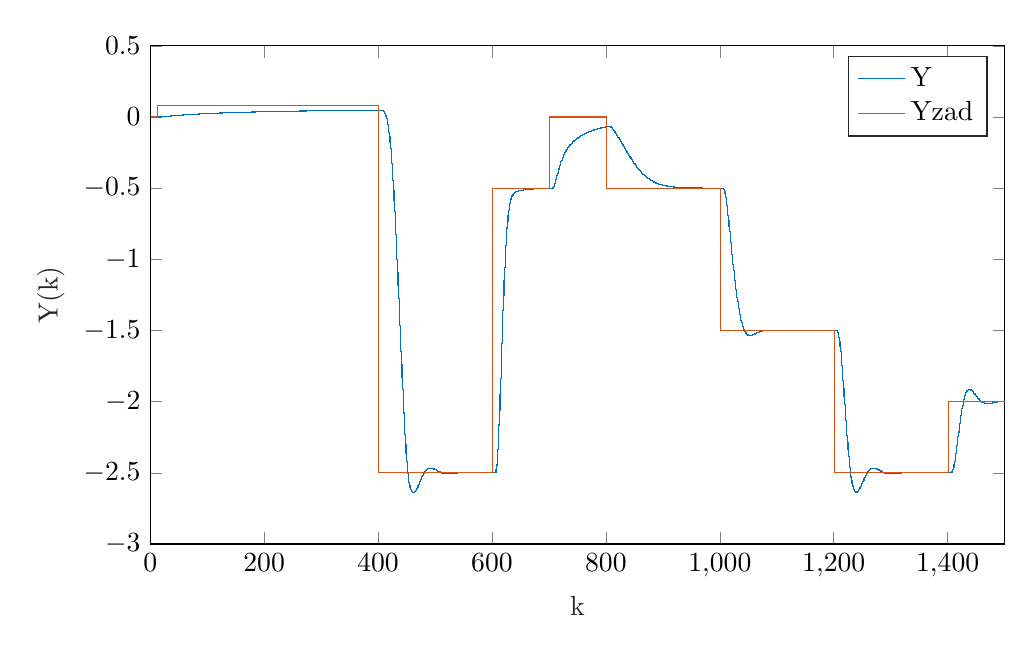
\begin{tikzpicture}

\begin{axis}[%
width=4.272in,
height=2.491in,
at={(0.717in,0.423in)},
scale only axis,
xmin=0,
xmax=1500,
xlabel style={font=\color{white!15!black}},
xlabel={k},
ymin=-3,
ymax=0.5,
ylabel style={font=\color{white!15!black}},
ylabel={Y(k)},
axis background/.style={fill=white},
legend style={legend cell align=left, align=left, draw=white!15!black}
]
\addplot[const plot, color=mycolor1] table[row sep=crcr] {%
1	0\\
2	0\\
3	0\\
4	0\\
5	0\\
6	0\\
7	0\\
8	0\\
9	0\\
10	0\\
11	0\\
12	0\\
13	0\\
14	0\\
15	0\\
16	0\\
17	5.82203665526567e-05\\
18	0.000227608410157792\\
19	0.000501157161978068\\
20	0.000850797033094626\\
21	0.00124711388384241\\
22	0.00166711803561433\\
23	0.00209561782716969\\
24	0.00252386446869852\\
25	0.0029475257926426\\
26	0.00336490418012234\\
27	0.00377566941345117\\
28	0.00418007933693575\\
29	0.00457856128369236\\
30	0.00497152227772156\\
31	0.00535928607067288\\
32	0.00574209030599219\\
33	0.00612010566338166\\
34	0.00649345820305135\\
35	0.00686224749673561\\
36	0.00722655891660137\\
37	0.00758647091818544\\
38	0.0079420588208698\\
39	0.00829339646082126\\
40	0.00864055671318002\\
41	0.00898361150589073\\
42	0.0093226316653438\\
43	0.00965768675267112\\
44	0.00998884494765684\\
45	0.0103161729879171\\
46	0.0106397361520534\\
47	0.0109595982717223\\
48	0.011275821759988\\
49	0.0115884676472896\\
50	0.0118975956198742\\
51	0.0122032640580413\\
52	0.0125055300730666\\
53	0.0128044495424873\\
54	0.0131000771437951\\
55	0.0133924663867073\\
56	0.0136816696441927\\
57	0.0139677381823964\\
58	0.0142507221895687\\
59	0.0145306708040711\\
60	0.0148076321415114\\
61	0.0150816533210458\\
62	0.0153527804908804\\
63	0.015621058853\\
64	0.0158865326871489\\
65	0.016149245374092\\
66	0.0164092394181763\\
67	0.0166665564692211\\
68	0.0169212373437564\\
69	0.0171733220456336\\
70	0.0174228497860298\\
71	0.0176698590028655\\
72	0.0179143873796569\\
73	0.0181564718638207\\
74	0.0183961486844509\\
75	0.0186334533695837\\
76	0.0188684207629698\\
77	0.0191010850403684\\
78	0.0193314797253797\\
79	0.0195596377048305\\
80	0.0197855912437284\\
81	0.0200093719997977\\
82	0.0202310110376106\\
83	0.0204505388423277\\
84	0.020667985333059\\
85	0.0208833798758588\\
86	0.0210967512963652\\
87	0.0213081278920956\\
88	0.0215175374444097\\
89	0.0217250072301497\\
90	0.0219305640329681\\
91	0.0221342341543526\\
92	0.0223360434243578\\
93	0.0225360172120527\\
94	0.0227341804356925\\
95	0.0229305575726229\\
96	0.0231251726689259\\
97	0.0233180493488143\\
98	0.0235092108237819\\
99	0.0236986799015189\\
100	0.0238864789945962\\
101	0.0240726301289291\\
102	0.0242571549520237\\
103	0.0244400747410152\\
104	0.0246214104105016\\
105	0.0248011825201818\\
106	0.0249794112823002\\
107	0.0251561165689068\\
108	0.0253313179189364\\
109	0.0255050345451119\\
110	0.0256772853406776\\
111	0.0258480888859673\\
112	0.0260174634548112\\
113	0.0261854270207866\\
114	0.0263519972633173\\
115	0.0265171915736247\\
116	0.0266810270605366\\
117	0.0268435205561551\\
118	0.0270046886213907\\
119	0.0271645475513635\\
120	0.0273231133806765\\
121	0.0274804018885644\\
122	0.0276364286039215\\
123	0.0277912088102114\\
124	0.0279447575502618\\
125	0.0280970896309482\\
126	0.0282482196277692\\
127	0.0283981618893152\\
128	0.0285469305416351\\
129	0.0286945394925032\\
130	0.0288410024355876\\
131	0.0289863328545245\\
132	0.0291305440269004\\
133	0.0292736490281436\\
134	0.0294156607353287\\
135	0.0295565918308959\\
136	0.0296964548062867\\
137	0.0298352619654993\\
138	0.0299730254285646\\
139	0.0301097571349461\\
140	0.0302454688468641\\
141	0.0303801721525481\\
142	0.0305138784694167\\
143	0.0306465990471897\\
144	0.0307783449709317\\
145	0.0309091271640301\\
146	0.0310389563911092\\
147	0.0311678432608816\\
148	0.0312957982289383\\
149	0.0314228316004797\\
150	0.0315489535329885\\
151	0.0316741740388459\\
152	0.0317985029878923\\
153	0.031921950109935\\
154	0.0320445249972024\\
155	0.0321662371067476\\
156	0.0322870957628016\\
157	0.0324071101590779\\
158	0.0325262893610294\\
159	0.0326446423080586\\
160	0.0327621778156829\\
161	0.0328789045776547\\
162	0.0329948311680397\\
163	0.0331099660432513\\
164	0.0332243175440447\\
165	0.0333378938974709\\
166	0.0334507032187909\\
167	0.0335627535133514\\
168	0.0336740526784234\\
169	0.0337846085050042\\
170	0.0338944286795829\\
171	0.0340035207858716\\
172	0.0341118923065027\\
173	0.0342195506246915\\
174	0.0343265030258677\\
175	0.0344327566992739\\
176	0.0345383187395338\\
177	0.0346431961481889\\
178	0.0347473958352068\\
179	0.0348509246204591\\
180	0.0349537892351715\\
181	0.0350559963233461\\
182	0.0351575524431561\\
183	0.0352584640683148\\
184	0.0353587375894172\\
185	0.0354583793152573\\
186	0.0355573954741205\\
187	0.0356557922150508\\
188	0.035753575609095\\
189	0.0358507516505233\\
190	0.0359473262580274\\
191	0.0360433052758958\\
192	0.0361386944751677\\
193	0.0362334995547659\\
194	0.0363277261426075\\
195	0.0364213797966962\\
196	0.0365144660061924\\
197	0.0366069901924657\\
198	0.0366989577101269\\
199	0.0367903738480418\\
200	0.0368812438303266\\
201	0.0369715728173251\\
202	0.0370613659065691\\
203	0.0371506281337202\\
204	0.037239364473496\\
205	0.0373275798405792\\
206	0.0374152790905108\\
207	0.0375024670205669\\
208	0.0375891483706205\\
209	0.0376753278239883\\
210	0.037761010008262\\
211	0.0378461994961252\\
212	0.0379309008061566\\
213	0.0380151184036181\\
214	0.0380988567012305\\
215	0.0381821200599344\\
216	0.0382649127896394\\
217	0.0383472391499587\\
218	0.0384291033509329\\
219	0.03851050955374\\
220	0.0385914618713935\\
221	0.0386719643694296\\
222	0.0387520210665813\\
223	0.038831635935442\\
224	0.0389108129031177\\
225	0.0389895558518679\\
226	0.0390678686197362\\
227	0.03914575500117\\
228	0.0392232187476298\\
229	0.0393002635681888\\
230	0.0393768931301218\\
231	0.039453111059485\\
232	0.0395289209416858\\
233	0.0396043263220435\\
234	0.0396793307063406\\
235	0.0397539375613648\\
236	0.0398281503154429\\
237	0.039901972358965\\
238	0.0399754070449013\\
239	0.0400484576893091\\
240	0.0401211275718331\\
241	0.0401934199361964\\
242	0.0402653379906845\\
243	0.0403368849086209\\
244	0.0404080638288351\\
245	0.040478877856124\\
246	0.0405493300617045\\
247	0.0406194234836603\\
248	0.0406891611273807\\
249	0.0407585459659927\\
250	0.0408275809407868\\
251	0.0408962689616351\\
252	0.0409646129074038\\
253	0.0410326156263588\\
254	0.0411002799365648\\
255	0.0411676086262786\\
256	0.0412346044543361\\
257	0.0413012701505334\\
258	0.0413676084160015\\
259	0.0414336219235762\\
260	0.0414993133181613\\
261	0.0415646852170871\\
262	0.0416297402104627\\
263	0.0416944808615234\\
264	0.0417589097069726\\
265	0.0418230292573185\\
266	0.0418868419972059\\
267	0.0419503503857427\\
268	0.0420135568568219\\
269	0.0420764638194381\\
270	0.042139073658\\
271	0.0422013887326378\\
272	0.0422634113795058\\
273	0.0423251439110813\\
274	0.042386588616458\\
275	0.0424477477616361\\
276	0.0425086235898074\\
277	0.0425692183216362\\
278	0.0426295341555368\\
279	0.0426895732679459\\
280	0.0427493378135919\\
281	0.0428088299257596\\
282	0.0428680517165517\\
283	0.0429270052771459\\
284	0.0429856926780487\\
285	0.0430441159693449\\
286	0.0431022771809447\\
287	0.0431601783228259\\
288	0.0432178213852734\\
289	0.0432752083391153\\
290	0.0433323411359551\\
291	0.0433892217084011\\
292	0.0434458519702922\\
293	0.0435022338169211\\
294	0.0435583691252531\\
295	0.0436142597541434\\
296	0.0436699075445499\\
297	0.0437253143197442\\
298	0.0437804818855186\\
299	0.043835412030391\\
300	0.0438901065258065\\
301	0.0439445671263364\\
302	0.0439987955698743\\
303	0.0440527935778295\\
304	0.0441065628553178\\
305	0.0441601050913499\\
306	0.0442134219590164\\
307	0.0442665151156713\\
308	0.044319386203112\\
309	0.044372036847758\\
310	0.0444244686608256\\
311	0.044476683238502\\
312	0.0445286821621154\\
313	0.044580466998304\\
314	0.0446320392991822\\
315	0.0446834006025042\\
316	0.0447345524318263\\
317	0.0447854962966664\\
318	0.0448362336926613\\
319	0.0448867661017221\\
320	0.0449370949921879\\
321	0.0449872218189764\\
322	0.0450371480237338\\
323	0.0450868750349817\\
324	0.0451364042682625\\
325	0.0451857371262828\\
326	0.0452348749990553\\
327	0.0452838192640376\\
328	0.0453325712862709\\
329	0.0453811324185156\\
330	0.0454295040013857\\
331	0.0454776873634812\\
332	0.0455256838215188\\
333	0.0455734946804614\\
334	0.0456211212336449\\
335	0.0456685647629045\\
336	0.0457158265386985\\
337	0.045762907820231\\
338	0.0458098098555731\\
339	0.0458565338817818\\
340	0.0459030811250183\\
341	0.0459494528006642\\
342	0.0459956501134367\\
343	0.0460416742575018\\
344	0.0460875264165862\\
345	0.0461332077640883\\
346	0.0461787194631872\\
347	0.0462240626669503\\
348	0.0462692385184402\\
349	0.0463142481508197\\
350	0.0463590926874554\\
351	0.0464037732420204\\
352	0.0464482909185958\\
353	0.0464926468117701\\
354	0.0465368420067385\\
355	0.0465808775794003\\
356	0.046624754596455\\
357	0.0466684741154975\\
358	0.0467120371851124\\
359	0.0467554448449663\\
360	0.0467986981258999\\
361	0.0468417980500183\\
362	0.0468847456307806\\
363	0.046927541873088\\
364	0.0469701877733713\\
365	0.0470126843196772\\
366	0.0470550324917533\\
367	0.0470972332611321\\
368	0.0471392875912146\\
369	0.0471811964373519\\
370	0.0472229607469269\\
371	0.0472645814594339\\
372	0.047306059506558\\
373	0.0473473958122538\\
374	0.0473885912928221\\
375	0.0474296468569867\\
376	0.0474705634059697\\
377	0.0475113418335661\\
378	0.047551983026218\\
379	0.0475924878630868\\
380	0.0476328572161254\\
381	0.0476730919501496\\
382	0.0477131929229083\\
383	0.0477531609851528\\
384	0.0477929969807058\\
385	0.0478327017465287\\
386	0.0478722761127897\\
387	0.047911720902929\\
388	0.0479510369337251\\
389	0.0479902250153592\\
390	0.0480292859514796\\
391	0.0480682205392645\\
392	0.0481070295694849\\
393	0.0481457138265664\\
394	0.0481842740886504\\
395	0.0482227111276543\\
396	0.0482610257093314\\
397	0.0482992185933302\\
398	0.0483372905332524\\
399	0.0483752422767107\\
400	0.0484130745653862\\
401	0.0484507881350845\\
402	0.0484883837157916\\
403	0.048525862031729\\
404	0.0485632238014086\\
405	0.048600469737686\\
406	0.0485631059350851\\
407	0.0474095766025166\\
408	0.045018246238092\\
409	0.0414302631737839\\
410	0.0366212759933214\\
411	0.0304562567805084\\
412	0.0226994045817526\\
413	0.0130371116839742\\
414	0.00110102715461315\\
415	-0.0135109797297391\\
416	-0.0312152938856005\\
417	-0.0524237768760867\\
418	-0.077525717468014\\
419	-0.1068710819096\\
420	-0.140755925185328\\
421	-0.179410806381526\\
422	-0.222992802418469\\
423	-0.271581348218188\\
424	-0.325177738473794\\
425	-0.383707795172346\\
426	-0.44702698680285\\
427	-0.514927194515025\\
428	-0.587144346889309\\
429	-0.663366259570418\\
430	-0.743240182071904\\
431	-0.826379735933877\\
432	-0.912371097563127\\
433	-1.00077841680967\\
434	-1.09114855983105\\
435	-1.18301532141369\\
436	-1.27590327262718\\
437	-1.36933140251055\\
438	-1.46281668639267\\
439	-1.55587767684885\\
440	-1.64803817319289\\
441	-1.73883098703822\\
442	-1.82780178830608\\
443	-1.91451299003448\\
444	-1.9985476121237\\
445	-2.07951305349653\\
446	-2.15704469819465\\
447	-2.23080928245613\\
448	-2.29976543978059\\
449	-2.36233565931744\\
450	-2.41752970813319\\
451	-2.46507776437185\\
452	-2.50519472212871\\
453	-2.53840132119216\\
454	-2.56539157459004\\
455	-2.58693724356246\\
456	-2.60382141747757\\
457	-2.61677610067711\\
458	-2.62638073833737\\
459	-2.63307769319252\\
460	-2.63721823734994\\
461	-2.63909448834129\\
462	-2.63896060636716\\
463	-2.63704632882945\\
464	-2.63356530470936\\
465	-2.6287199641534\\
466	-2.62270410511948\\
467	-2.61570400050082\\
468	-2.60789857278287\\
469	-2.59945900982916\\
470	-2.59054807745958\\
471	-2.58131930362232\\
472	-2.57191615289416\\
473	-2.56247127065382\\
474	-2.55310584818945\\
475	-2.5439291396803\\
476	-2.53503814709512\\
477	-2.52651747803104\\
478	-2.51843937335399\\
479	-2.51086389550842\\
480	-2.50383926407095\\
481	-2.49740232219516\\
482	-2.49157911578162\\
483	-2.48638556631104\\
484	-2.48182821812883\\
485	-2.47790504142209\\
486	-2.4746062730513\\
487	-2.47191527867194\\
488	-2.46980942109793\\
489	-2.46826092152835\\
490	-2.46723770199906\\
491	-2.46670419916772\\
492	-2.46662214123945\\
493	-2.46695128145235\\
494	-2.46765008303812\\
495	-2.46867635193443\\
496	-2.46998781474471\\
497	-2.47154264051351\\
498	-2.47329990581581\\
499	-2.47522000345468\\
500	-2.47726499573172\\
501	-2.47939891381235\\
502	-2.48158800516485\\
503	-2.48380093141962\\
504	-2.48600891928689\\
505	-2.48818586739567\\
506	-2.49030841208552\\
507	-2.49235595530231\\
508	-2.49431065782784\\
509	-2.49615740111586\\
510	-2.49788372101836\\
511	-2.49947971667073\\
512	-2.50093793776342\\
513	-2.5022532533659\\
514	-2.50342270538548\\
515	-2.50444534964238\\
516	-2.50532208742334\\
517	-2.50605549024153\\
518	-2.5066496203806\\
519	-2.50710984963834\\
520	-2.50744267851072\\
521	-2.50765555787292\\
522	-2.50775671502128\\
523	-2.50775498574153\\
524	-2.5076596538663\\
525	-2.50748029958005\\
526	-2.50722665752606\\
527	-2.5069084855683\\
528	-2.50653544486469\\
529	-2.5061169917183\\
530	-2.50566228149213\\
531	-2.50518008470226\\
532	-2.5046787152456\\
533	-2.50416597057297\\
534	-2.5036490834865\\
535	-2.50313468512431\\
536	-2.50262877859375\\
537	-2.50213672262889\\
538	-2.50166322457777\\
539	-2.50121234196942\\
540	-2.50078749187015\\
541	-2.50039146721192\\
542	-2.50002645926159\\
543	-2.49969408539857\\
544	-2.49939542137709\\
545	-2.49913103726897\\
546	-2.49890103630996\\
547	-2.49870509590813\\
548	-2.49854251011412\\
549	-2.49841223289925\\
550	-2.49831292163819\\
551	-2.49824298024588\\
552	-2.49820060147373\\
553	-2.49818380792623\\
554	-2.49819049141534\\
555	-2.49821845032601\\
556	-2.49826542472053\\
557	-2.49832912896206\\
558	-2.49840728168842\\
559	-2.49849763301477\\
560	-2.49859798888847\\
561	-2.49870623256132\\
562	-2.49882034318182\\
563	-2.49893841154506\\
564	-2.49905865306845\\
565	-2.4991794180885\\
566	-2.49929919959769\\
567	-2.4994166385601\\
568	-2.49953052696103\\
569	-2.49963980875889\\
570	-2.49974357891763\\
571	-2.49984108070472\\
572	-2.49993170144384\\
573	-2.50001496691293\\
574	-2.50009053457707\\
575	-2.50015818584294\\
576	-2.50021781751613\\
577	-2.50026943263612\\
578	-2.50031313085538\\
579	-2.50034909851953\\
580	-2.50037759859514\\
581	-2.50039896058029\\
582	-2.50041357052106\\
583	-2.50042186124502\\
584	-2.50042430290985\\
585	-2.50042139395308\\
586	-2.50041365251581\\
587	-2.50040160840162\\
588	-2.50038579561941\\
589	-2.50036674554787\\
590	-2.50034498074809\\
591	-2.50032100944079\\
592	-2.50029532065509\\
593	-2.5002683800469\\
594	-2.50024062637726\\
595	-2.50021246863364\\
596	-2.50018428377115\\
597	-2.500156415045\\
598	-2.5001291709011\\
599	-2.50010282438787\\
600	-2.50007761304939\\
601	-2.50005373925761\\
602	-2.50003137094012\\
603	-2.50001064265888\\
604	-2.49999165699519\\
605	-2.49997448619644\\
606	-2.49409755539735\\
607	-2.47678793285635\\
608	-2.44491817833711\\
609	-2.39719720544448\\
610	-2.33367647420253\\
611	-2.25537039890068\\
612	-2.16397506252028\\
613	-2.06165673180075\\
614	-1.95088489059753\\
615	-1.83429235421586\\
616	-1.71455210596572\\
617	-1.59426596888675\\
618	-1.47586427530434\\
619	-1.36151852229958\\
620	-1.25307063697277\\
621	-1.15198286901688\\
622	-1.0593114926957\\
623	-0.97570562711284\\
624	-0.901430018768432\\
625	-0.836408136027065\\
626	-0.780279970102391\\
627	-0.732467915955886\\
628	-0.692244141112081\\
629	-0.658793795840998\\
630	-0.631269950246736\\
631	-0.608837882305527\\
632	-0.590707957380295\\
633	-0.576157619574169\\
634	-0.564543869731547\\
635	-0.555308047456892\\
636	-0.547974841765565\\
637	-0.54214732841347\\
638	-0.537499570060413\\
639	-0.533767998086565\\
640	-0.530742478108653\\
641	-0.528257678585604\\
642	-0.526185129142345\\
643	-0.524426175862753\\
644	-0.522905910894511\\
645	-0.521568065688293\\
646	-0.520370802335726\\
647	-0.519283307411148\\
648	-0.518283080220898\\
649	-0.517353806574854\\
650	-0.516483715649741\\
651	-0.515664327958413\\
652	-0.514889514615143\\
653	-0.514154800508496\\
654	-0.513456855749822\\
655	-0.512793130355456\\
656	-0.512161596323197\\
657	-0.511560569039234\\
658	-0.51098858637197\\
659	-0.51044432900659\\
660	-0.509926569708121\\
661	-0.509434142435825\\
662	-0.508965924724715\\
663	-0.508520828642381\\
664	-0.50809779704417\\
665	-0.507695802891233\\
666	-0.507313850149814\\
667	-0.506950975326021\\
668	-0.506606249063267\\
669	-0.506278777482897\\
670	-0.505967703115317\\
671	-0.505672205374451\\
672	-0.505391500591252\\
673	-0.505124841656173\\
674	-0.504871517335742\\
675	-0.504630851331884\\
676	-0.504402201149076\\
677	-0.504184956827256\\
678	-0.503978539589629\\
679	-0.50378240044555\\
680	-0.503596018780244\\
681	-0.503418900955645\\
682	-0.503250578940285\\
683	-0.503090608980899\\
684	-0.502938570324253\\
685	-0.502794063994355\\
686	-0.502656711627778\\
687	-0.502526154367895\\
688	-0.502402051817554\\
689	-0.502284081048732\\
690	-0.502171935667136\\
691	-0.502065324929309\\
692	-0.501963972909631\\
693	-0.501867617714471\\
694	-0.501776010740825\\
695	-0.501688915976774\\
696	-0.501606109341264\\
697	-0.501527378060777\\
698	-0.501452520080656\\
699	-0.501381343508945\\
700	-0.501313666090759\\
701	-0.501249314711352\\
702	-0.501188124926131\\
703	-0.501129940516037\\
704	-0.501074613066778\\
705	-0.501022001570534\\
706	-0.499642785686346\\
707	-0.495882932280213\\
708	-0.489392898734314\\
709	-0.480278715915132\\
710	-0.468907759271521\\
711	-0.455769150459156\\
712	-0.441381034772152\\
713	-0.426233277104159\\
714	-0.41075533471758\\
715	-0.395301467649411\\
716	-0.380147528724972\\
717	-0.365495132766198\\
718	-0.351480144663456\\
719	-0.338183276544137\\
720	-0.325641237392536\\
721	-0.313857390028181\\
722	-0.302811272163362\\
723	-0.292466646474463\\
724	-0.282777974665349\\
725	-0.273695370483772\\
726	-0.265168187626772\\
727	-0.257147452210469\\
728	-0.249587367346701\\
729	-0.242446110048705\\
730	-0.235686117525939\\
731	-0.229274028523839\\
732	-0.223180411436123\\
733	-0.217379378394225\\
734	-0.211848155803375\\
735	-0.206566658003691\\
736	-0.201517092149708\\
737	-0.196683608696492\\
738	-0.192052002392815\\
739	-0.187609462607066\\
740	-0.183344368336565\\
741	-0.179246121637907\\
742	-0.175305012845706\\
743	-0.171512111333205\\
744	-0.167859176351941\\
745	-0.164338583421808\\
746	-0.160943262670431\\
747	-0.157666646353261\\
748	-0.154502623483127\\
749	-0.151445500051797\\
750	-0.148489963746873\\
751	-0.145631052374873\\
752	-0.142864125418511\\
753	-0.140184838304904\\
754	-0.137589119060856\\
755	-0.135073147096816\\
756	-0.132633333904239\\
757	-0.13026630548025\\
758	-0.127968886314339\\
759	-0.125738084787958\\
760	-0.123571079851439\\
761	-0.121465208854823\\
762	-0.119417956420473\\
763	-0.117426944256011\\
764	-0.115489921816089\\
765	-0.113604757730858\\
766	-0.111769431927543\\
767	-0.109982028379377\\
768	-0.108240728423123\\
769	-0.106543804592759\\
770	-0.104889614922415\\
771	-0.103276597676621\\
772	-0.101703266470262\\
773	-0.100168205744472\\
774	-0.0986700665680857\\
775	-0.0972075627372766\\
776	-0.0957794671486364\\
777	-0.0943846084233403\\
778	-0.0930218677621165\\
779	-0.0916901760126272\\
780	-0.0903885109325406\\
781	-0.0891158946330785\\
782	-0.0878713911891768\\
783	-0.0866541044036089\\
784	-0.0854631757135231\\
785	-0.0842977822288304\\
786	-0.0831571348927746\\
787	-0.0820404767558277\\
788	-0.0809470813547832\\
789	-0.0798762511895879\\
790	-0.0788273162910556\\
791	-0.0777996328731536\\
792	-0.0767925820640552\\
793	-0.0758055687106042\\
794	-0.074838020251253\\
795	-0.0738893856529151\\
796	-0.0729591344075191\\
797	-0.0720467555843669\\
798	-0.0711517569346903\\
799	-0.0702736640450643\\
800	-0.0694120195365802\\
801	-0.0685663823069051\\
802	-0.06773632681256\\
803	-0.066921442388937\\
804	-0.0661213326057518\\
805	-0.0653356146557867\\
806	-0.0652501293417874\\
807	-0.0663871058620391\\
808	-0.0687789901061393\\
809	-0.0722391254762623\\
810	-0.0765197054624519\\
811	-0.0813909797644232\\
812	-0.0866713416531959\\
813	-0.0922310269847433\\
814	-0.0979842341513565\\
815	-0.103877938073753\\
816	-0.109881370492458\\
817	-0.115977655054174\\
818	-0.122157813665344\\
819	-0.128416810268925\\
820	-0.134751136354356\\
821	-0.141157464975834\\
822	-0.147631992046011\\
823	-0.154170188580448\\
824	-0.160766777677618\\
825	-0.167415819228215\\
826	-0.174110834265632\\
827	-0.180844932876558\\
828	-0.187610929165793\\
829	-0.194401437862969\\
830	-0.201208952833435\\
831	-0.20802591019138\\
832	-0.214844739360802\\
833	-0.22165790519564\\
834	-0.228457943684521\\
835	-0.235237493113224\\
836	-0.241989321974437\\
837	-0.248706354449117\\
838	-0.255381693941243\\
839	-0.262008644912133\\
840	-0.2685807331092\\
841	-0.275091724194872\\
842	-0.281535640735542\\
843	-0.28790677749307\\
844	-0.294199714961878\\
845	-0.300409331105491\\
846	-0.306530811262507\\
847	-0.312559656210244\\
848	-0.31849168839284\\
849	-0.324323056338181\\
850	-0.330050237304207\\
851	-0.335670038209582\\
852	-0.341179594916403\\
853	-0.346576369943474\\
854	-0.351858148697878\\
855	-0.35702303432011\\
856	-0.362069441244102\\
857	-0.366996087578006\\
858	-0.371801986414882\\
859	-0.376486436184393\\
860	-0.381049010157391\\
861	-0.38548954521501\\
862	-0.389808129992549\\
863	-0.394005092506234\\
864	-0.398080987367904\\
865	-0.402036582688878\\
866	-0.405872846769883\\
867	-0.409590934668934\\
868	-0.413192174733657\\
869	-0.416678055178796\\
870	-0.420050210783535\\
871	-0.42331040977709\\
872	-0.426460540974588\\
873	-0.429502601218915\\
874	-0.432438683177775\\
875	-0.435270963538953\\
876	-0.438001691640618\\
877	-0.440633178567539\\
878	-0.443167786738388\\
879	-0.445607920003861\\
880	-0.447956014270208\\
881	-0.450214528657953\\
882	-0.452385937201121\\
883	-0.454472721088195\\
884	-0.456477361442247\\
885	-0.458402332634351\\
886	-0.460250096121343\\
887	-0.462023094796331\\
888	-0.463723747838076\\
889	-0.465354446043345\\
890	-0.466917547624716\\
891	-0.468415374454942\\
892	-0.469850208737898\\
893	-0.471224290085354\\
894	-0.472539812978224\\
895	-0.473798924590615\\
896	-0.475003722954851\\
897	-0.476156255445686\\
898	-0.477258517562124\\
899	-0.478312451985601\\
900	-0.479319947893744\\
901	-0.480282840509487\\
902	-0.481202910865992\\
903	-0.482081885768508\\
904	-0.482921437935137\\
905	-0.483723186299238\\
906	-0.484488696457113\\
907	-0.485219481245432\\
908	-0.485917001433803\\
909	-0.486582666518721\\
910	-0.487217835606041\\
911	-0.487823818369988\\
912	-0.488401876077537\\
913	-0.488953222667872\\
914	-0.489479025877364\\
915	-0.489980408401348\\
916	-0.490458449084664\\
917	-0.490914184133652\\
918	-0.491348608342957\\
919	-0.491762676331127\\
920	-0.492157303779589\\
921	-0.492533368670138\\
922	-0.49289171251661\\
923	-0.493233141586879\\
924	-0.493558428111804\\
925	-0.493868311478129\\
926	-0.494163499402775\\
927	-0.494444669086284\\
928	-0.494712468343517\\
929	-0.494967516710028\\
930	-0.495210406522767\\
931	-0.49544170397406\\
932	-0.495661950138014\\
933	-0.495871661968707\\
934	-0.496071333269705\\
935	-0.496261435634613\\
936	-0.496442419358528\\
937	-0.496614714320356\\
938	-0.496778730836122\\
939	-0.496934860483459\\
940	-0.497083476897575\\
941	-0.497224936539067\\
942	-0.49735957943403\\
943	-0.497487729886931\\
944	-0.49760969716682\\
945	-0.497725776167433\\
946	-0.497836248041828\\
947	-0.497941380812174\\
948	-0.498041429955367\\
949	-0.49813663896515\\
950	-0.498227239891427\\
951	-0.49831345385745\\
952	-0.49839549155561\\
953	-0.498473553722486\\
954	-0.49854783159389\\
955	-0.498618507340563\\
956	-0.498685754485217\\
957	-0.498749738301598\\
958	-0.498810616196217\\
959	-0.498868538073412\\
960	-0.498923646684356\\
961	-0.498976077960649\\
962	-0.499025961333085\\
963	-0.499073420036184\\
964	-0.499118571399065\\
965	-0.499161527123216\\
966	-0.499202393547681\\
967	-0.499241271902219\\
968	-0.499278258548902\\
969	-0.499313445212671\\
970	-0.499346919201294\\
971	-0.499378763615204\\
972	-0.499409057547635\\
973	-0.49943787627549\\
974	-0.499465291441343\\
975	-0.49949137122696\\
976	-0.499516180518729\\
977	-0.499539781065336\\
978	-0.499562231628064\\
979	-0.499583588124013\\
980	-0.49960390376259\\
981	-0.499623229175557\\
982	-0.49964161254093\\
983	-0.499659099701025\\
984	-0.499675734274897\\
985	-0.499691557765449\\
986	-0.499706609661447\\
987	-0.499720927534679\\
988	-0.49973454713248\\
989	-0.49974750246585\\
990	-0.49975982589335\\
991	-0.499771548200998\\
992	-0.499782698678331\\
993	-0.499793305190823\\
994	-0.499803394248835\\
995	-0.499812991073249\\
996	-0.499822119657948\\
997	-0.499830802829294\\
998	-0.499839062302745\\
999	-0.499846918736738\\
1000	-0.499854391783984\\
1001	-0.499861500140283\\
1002	-0.499868261590987\\
1003	-0.499874693055215\\
1004	-0.499880810627941\\
1005	-0.499886629620034\\
1006	-0.502500206667808\\
1007	-0.509777009957502\\
1008	-0.522459869687423\\
1009	-0.54049983290263\\
1010	-0.563421943365344\\
1011	-0.590561939338188\\
1012	-0.621206232820208\\
1013	-0.654667240491498\\
1014	-0.690318735126383\\
1015	-0.727607978711876\\
1016	-0.766055330470602\\
1017	-0.805247841784332\\
1018	-0.844830615759441\\
1019	-0.88449798712839\\
1020	-0.923985532009318\\
1021	-0.963063307708575\\
1022	-1.00153038658933\\
1023	-1.03921058146208\\
1024	-1.07594918703963\\
1025	-1.11161054403555\\
1026	-1.14607624295777\\
1027	-1.17924380733939\\
1028	-1.21102572255197\\
1029	-1.2413487020468\\
1030	-1.27015310585229\\
1031	-1.29739244574092\\
1032	-1.32303292768959\\
1033	-1.34705299543346\\
1034	-1.3694428495134\\
1035	-1.39020392469918\\
1036	-1.40934831544513\\
1037	-1.42689814444497\\
1038	-1.44288487366937\\
1039	-1.45734856070462\\
1040	-1.47033706592104\\
1041	-1.48190521810032\\
1042	-1.4921139477292\\
1043	-1.5010293982819\\
1044	-1.50872202651571\\
1045	-1.51526570312843\\
1046	-1.52073682510839\\
1047	-1.52521345077706\\
1048	-1.52877446791612\\
1049	-1.5314988045177\\
1050	-1.53346469063886\\
1051	-1.53474897861793\\
1052	-1.53542652756582\\
1053	-1.53556965662321\\
1054	-1.53524767001893\\
1055	-1.5345264555194\\
1056	-1.53346815646296\\
1057	-1.53213091626233\\
1058	-1.5305686930643\\
1059	-1.52883114120199\\
1060	-1.52696355518023\\
1061	-1.5250068712091\\
1062	-1.5229977207502\\
1063	-1.52096853016174\\
1064	-1.5189476603162\\
1065	-1.51695958000514\\
1066	-1.51502506702575\\
1067	-1.51316143104279\\
1068	-1.51138275262057\\
1069	-1.50970013319987\\
1070	-1.50812195123589\\
1071	-1.5066541201954\\
1072	-1.50530034461693\\
1073	-1.50406237095146\\
1074	-1.50294023040872\\
1075	-1.50193247152541\\
1076	-1.50103638063665\\
1077	-1.50024818886456\\
1078	-1.49956326463332\\
1079	-1.49897629107536\\
1080	-1.49848142800724\\
1081	-1.49807245842669\\
1082	-1.49774291971464\\
1083	-1.49748621992053\\
1084	-1.49729573966774\\
1085	-1.4971649203418\\
1086	-1.49708733932018\\
1087	-1.49705677307223\\
1088	-1.49706724900431\\
1089	-1.4971130869516\\
1090	-1.4971889312272\\
1091	-1.49728977413425\\
1092	-1.49741097182902\\
1093	-1.49754825339675\\
1094	-1.49769772396688\\
1095	-1.49785586265405\\
1096	-1.49801951606627\\
1097	-1.49818588807367\\
1098	-1.49835252648121\\
1099	-1.49851730719793\\
1100	-1.49867841644428\\
1101	-1.49883433148823\\
1102	-1.49898380035186\\
1103	-1.4991258208816\\
1104	-1.49925961952978\\
1105	-1.49938463015058\\
1106	-1.49950047307263\\
1107	-1.4996069346708\\
1108	-1.49970394762387\\
1109	-1.49979157201075\\
1110	-1.49986997736706\\
1111	-1.49993942579571\\
1112	-1.50000025619922\\
1113	-1.50005286967904\\
1114	-1.5000977161261\\
1115	-1.50013528200935\\
1116	-1.50016607935302\\
1117	-1.50019063587995\\
1118	-1.50020948628701\\
1119	-1.50022316460907\\
1120	-1.50023219762035\\
1121	-1.50023709921591\\
1122	-1.50023836571161\\
1123	-1.50023647199763\\
1124	-1.50023186847881\\
1125	-1.50022497873403\\
1126	-1.50021619782729\\
1127	-1.50020589120367\\
1128	-1.50019439410538\\
1129	-1.50018201144506\\
1130	-1.50016901807633\\
1131	-1.50015565940465\\
1132	-1.50014215228494\\
1133	-1.5001286861562\\
1134	-1.50011542436663\\
1135	-1.50010250564728\\
1136	-1.50009004569549\\
1137	-1.50007813883352\\
1138	-1.50006685971138\\
1139	-1.50005626502661\\
1140	-1.50004639523703\\
1141	-1.500037276246\\
1142	-1.50002892104272\\
1143	-1.50002133128305\\
1144	-1.50001449879909\\
1145	-1.5000084070281\\
1146	-1.50000303235385\\
1147	-1.49999834535525\\
1148	-1.49999431195922\\
1149	-1.49999089449627\\
1150	-1.49998805265858\\
1151	-1.49998574436181\\
1152	-1.49998392651287\\
1153	-1.49998255568654\\
1154	-1.49998158871503\\
1155	-1.49998098319458\\
1156	-1.49998069791411\\
1157	-1.49998069321104\\
1158	-1.49998093125958\\
1159	-1.49998137629712\\
1160	-1.49998199479415\\
1161	-1.49998275557318\\
1162	-1.49998362988218\\
1163	-1.49998459142764\\
1164	-1.49998561637232\\
1165	-1.49998668330255\\
1166	-1.49998777316952\\
1167	-1.49998886920881\\
1168	-1.49998995684222\\
1169	-1.49999102356535\\
1170	-1.49999205882443\\
1171	-1.49999305388527\\
1172	-1.49999400169708\\
1173	-1.49999489675364\\
1174	-1.49999573495375\\
1175	-1.49999651346296\\
1176	-1.49999723057811\\
1177	-1.49999788559588\\
1178	-1.49999847868665\\
1179	-1.49999901077439\\
1180	-1.4999994834233\\
1181	-1.49999989873177\\
1182	-1.50000025923392\\
1183	-1.50000056780903\\
1184	-1.50000082759876\\
1185	-1.50000104193238\\
1186	-1.50000121425967\\
1187	-1.5000013480914\\
1188	-1.50000144694702\\
1189	-1.50000151430944\\
1190	-1.5000015535862\\
1191	-1.50000156807695\\
1192	-1.50000156094667\\
1193	-1.50000153520411\\
1194	-1.50000149368518\\
1195	-1.50000143904071\\
1196	-1.50000137372824\\
1197	-1.50000130000723\\
1198	-1.50000121993753\\
1199	-1.50000113538047\\
1200	-1.50000104800234\\
1201	-1.50000095927981\\
1202	-1.50000087050703\\
1203	-1.50000078280404\\
1204	-1.50000069712624\\
1205	-1.50000061427461\\
1206	-1.50285955091034\\
1207	-1.51107392073317\\
1208	-1.52585846977265\\
1209	-1.54756303532419\\
1210	-1.57598681858739\\
1211	-1.61060094723734\\
1212	-1.65069711864779\\
1213	-1.69548329762324\\
1214	-1.74414366086094\\
1215	-1.79587502300019\\
1216	-1.84990805960222\\
1217	-1.90551888542204\\
1218	-1.9620346669406\\
1219	-2.0188356763438\\
1220	-2.07535533512222\\
1221	-2.13107921741853\\
1222	-2.185543596606\\
1223	-2.23833386694742\\
1224	-2.28908300732055\\
1225	-2.33747015136802\\
1226	-2.38321926779819\\
1227	-2.42606575123612\\
1228	-2.46510580707535\\
1229	-2.4996599373263\\
1230	-2.52951353487681\\
1231	-2.5547668581442\\
1232	-2.57572085199412\\
1233	-2.59279224302658\\
1234	-2.60645022211028\\
1235	-2.61709106738716\\
1236	-2.62502839293801\\
1237	-2.63052206929977\\
1238	-2.63379857125231\\
1239	-2.63506437794738\\
1240	-2.63451426753831\\
1241	-2.63233612421105\\
1242	-2.62871342433102\\
1243	-2.62382620120797\\
1244	-2.61785103508859\\
1245	-2.61096044317619\\
1246	-2.60332192805442\\
1247	-2.59509686351654\\
1248	-2.58643934204684\\
1249	-2.57749506982461\\
1250	-2.56840036770499\\
1251	-2.55928131662185\\
1252	-2.55025307093365\\
1253	-2.54141935188534\\
1254	-2.53287212460986\\
1255	-2.52469145530975\\
1256	-2.51694554002986\\
1257	-2.50969089247945\\
1258	-2.50297267549191\\
1259	-2.49682515877232\\
1260	-2.49127228445327\\
1261	-2.48632832154368\\
1262	-2.48199859050675\\
1263	-2.47828023983712\\
1264	-2.47516305752387\\
1265	-2.47263030158956\\
1266	-2.47065953539865\\
1267	-2.46922345505137\\
1268	-2.46829069785407\\
1269	-2.46782662252517\\
1270	-2.46779405341209\\
1271	-2.46815398252333\\
1272	-2.46886622459627\\
1273	-2.4698900217101\\
1274	-2.47118459510587\\
1275	-2.47270964289155\\
1276	-2.47442578319132\\
1277	-2.47629494305349\\
1278	-2.47828069406894\\
1279	-2.48034853618328\\
1280	-2.48246613162207\\
1281	-2.48460349120127\\
1282	-2.4867331155747\\
1283	-2.48883009418751\\
1284	-2.49087216486708\\
1285	-2.49283973709917\\
1286	-2.49471588211321\\
1287	-2.49648629294187\\
1288	-2.49813921763126\\
1289	-2.49966536876183\\
1290	-2.50105781240031\\
1291	-2.502311839541\\
1292	-2.50342482301286\\
1293	-2.50439606272857\\
1294	-2.50522662203455\\
1295	-2.50591915778781\\
1296	-2.5064777466387\\
1297	-2.50690770983873\\
1298	-2.50721543872146\\
1299	-2.50740822282472\\
1300	-2.50749408243378\\
1301	-2.50748160713249\\
1302	-2.50737980175188\\
1303	-2.50719794090789\\
1304	-2.5069454331224\\
1305	-2.50663169532705\\
1306	-2.50626603836036\\
1307	-2.50585756388557\\
1308	-2.50541507298342\\
1309	-2.50494698651022\\
1310	-2.50446127716026\\
1311	-2.50396541303267\\
1312	-2.50346631237782\\
1313	-2.502970309088\\
1314	-2.50248312840123\\
1315	-2.50200987220641\\
1316	-2.50155501327197\\
1317	-2.5011223976687\\
1318	-2.50071525462024\\
1319	-2.50033621299008\\
1320	-2.49998732360257\\
1321	-2.49967008659485\\
1322	-2.49938548300688\\
1323	-2.49913400983609\\
1324	-2.49891571781082\\
1325	-2.49873025117135\\
1326	-2.49857688878767\\
1327	-2.49845458598853\\
1328	-2.49836201652523\\
1329	-2.49829761414497\\
1330	-2.4982596133024\\
1331	-2.49824608859164\\
1332	-2.49825499253589\\
1333	-2.49828419142505\\
1334	-2.49833149894428\\
1335	-2.49839470738729\\
1336	-2.49847161629615\\
1337	-2.49856005841571\\
1338	-2.49865792289302\\
1339	-2.49876317569236\\
1340	-2.49887387723237\\
1341	-2.49898819728501\\
1342	-2.4991044272052\\
1343	-2.49922098958593\\
1344	-2.49933644545595\\
1345	-2.49944949915582\\
1346	-2.49955900104392\\
1347	-2.49966394819608\\
1348	-2.49976348327171\\
1349	-2.4998568917259\\
1350	-2.49994359755021\\
1351	-2.50002315772633\\
1352	-2.50009525557546\\
1353	-2.50015969318305\\
1354	-2.50021638307349\\
1355	-2.50026533930255\\
1356	-2.50030666812753\\
1357	-2.50034055840538\\
1358	-2.50036727185917\\
1359	-2.50038713334216\\
1360	-2.50040052121699\\
1361	-2.50040785795585\\
1362	-2.50040960105519\\
1363	-2.50040623434615\\
1364	-2.50039825977028\\
1365	-2.50038618967782\\
1366	-2.50037053969457\\
1367	-2.50035182219245\\
1368	-2.50033054038813\\
1369	-2.5003071830846\\
1370	-2.50028222006141\\
1371	-2.50025609811065\\
1372	-2.50022923770863\\
1373	-2.50020203030613\\
1374	-2.50017483621417\\
1375	-2.50014798305727\\
1376	-2.5001217647617\\
1377	-2.50009644104263\\
1378	-2.50007223735144\\
1379	-2.5000493452423\\
1380	-2.50002792311567\\
1381	-2.50000809729574\\
1382	-2.49998996339866\\
1383	-2.49997358794866\\
1384	-2.49995901020012\\
1385	-2.49994624412507\\
1386	-2.49993528052692\\
1387	-2.49992608924363\\
1388	-2.49991862140548\\
1389	-2.49991281171519\\
1390	-2.49990858072082\\
1391	-2.49990583705466\\
1392	-2.4999044796139\\
1393	-2.49990439966227\\
1394	-2.49990548283403\\
1395	-2.49990761102517\\
1396	-2.49991066415901\\
1397	-2.49991452181616\\
1398	-2.49991906472153\\
1399	-2.49992417608313\\
1400	-2.49992974278002\\
1401	-2.49993565639856\\
1402	-2.49994181411826\\
1403	-2.4999481194499\\
1404	-2.4999544828306\\
1405	-2.49996082208127\\
1406	-2.49852225564395\\
1407	-2.49429145186406\\
1408	-2.48653313636747\\
1409	-2.47495411721108\\
1410	-2.45956887504051\\
1411	-2.44059898518055\\
1412	-2.41840119986048\\
1413	-2.39341652528818\\
1414	-2.36613373271541\\
1415	-2.33706269465275\\
1416	-2.3067145195144\\
1417	-2.27558654495483\\
1418	-2.24415095491147\\
1419	-2.21284622906926\\
1420	-2.18207090587036\\
1421	-2.15217930186372\\
1422	-2.12347892176601\\
1423	-2.09622933967193\\
1424	-2.07064235436214\\
1425	-2.04688323017911\\
1426	-2.02507283784005\\
1427	-2.00529051237478\\
1428	-1.98757745098619\\
1429	-1.97194048329122\\
1430	-1.95835606022144\\
1431	-1.94677432520259\\
1432	-1.93712315102686\\
1433	-1.92931204684993\\
1434	-1.92323586078999\\
1435	-1.91877822364561\\
1436	-1.91581469748528\\
1437	-1.91421560876406\\
1438	-1.91384855891026\\
1439	-1.91458061594105\\
1440	-1.91628019872248\\
1441	-1.91881867122474\\
1442	-1.92207166784801\\
1443	-1.92592017295417\\
1444	-1.9302513784816\\
1445	-1.93495934326897\\
1446	-1.93994547675884\\
1447	-1.94511886833723\\
1448	-1.95039648188951\\
1449	-1.95570323336961\\
1450	-1.96097196740181\\
1451	-1.96614334724044\\
1452	-1.97116567085135\\
1453	-1.97599462447778\\
1454	-1.980592983819\\
1455	-1.98493027188112\\
1456	-1.98898238164205\\
1457	-1.99273117088977\\
1458	-1.99616403592431\\
1459	-1.99927347023801\\
1460	-2.00205661378576\\
1461	-2.00451479800727\\
1462	-2.00665309135212\\
1463	-2.00847984966956\\
1464	-2.01000627545004\\
1465	-2.01124598953393\\
1466	-2.01221461853058\\
1467	-2.01292940081463\\
1468	-2.01340881358384\\
1469	-2.01367222307681\\
1470	-2.0137395596594\\
1471	-2.01363101910131\\
1472	-2.01336679098097\\
1473	-2.01296681478436\\
1474	-2.01245056390416\\
1475	-2.01183685740676\\
1476	-2.01114369911775\\
1477	-2.01038814328813\\
1478	-2.00958618584414\\
1479	-2.008752679998\\
1480	-2.0079012748044\\
1481	-2.0070443750913\\
1482	-2.0061931210713\\
1483	-2.0053573858526\\
1484	-2.00454578901381\\
1485	-2.00376572438323\\
1486	-2.00302340016799\\
1487	-2.00232388960917\\
1488	-2.00167119039213\\
1489	-2.00106829111423\\
1490	-2.00051724320121\\
1491	-2.00001923676587\\
1492	-1.99957467901486\\
1493	-1.99918327392896\\
1494	-1.99884410206617\\
1495	-1.99855569946266\\
1496	-1.99831613473265\\
1497	-1.99812308359165\\
1498	-1.99797390014776\\
1499	-1.9978656844206\\
1500	-1.99779534565631\\
};
\addlegendentry{Y}

\addplot[const plot, color=mycolor2] table[row sep=crcr] {%
1	0\\
2	0\\
3	0\\
4	0\\
5	0\\
6	0\\
7	0\\
8	0\\
9	0\\
10	0\\
11	0\\
12	0.08\\
13	0.08\\
14	0.08\\
15	0.08\\
16	0.08\\
17	0.08\\
18	0.08\\
19	0.08\\
20	0.08\\
21	0.08\\
22	0.08\\
23	0.08\\
24	0.08\\
25	0.08\\
26	0.08\\
27	0.08\\
28	0.08\\
29	0.08\\
30	0.08\\
31	0.08\\
32	0.08\\
33	0.08\\
34	0.08\\
35	0.08\\
36	0.08\\
37	0.08\\
38	0.08\\
39	0.08\\
40	0.08\\
41	0.08\\
42	0.08\\
43	0.08\\
44	0.08\\
45	0.08\\
46	0.08\\
47	0.08\\
48	0.08\\
49	0.08\\
50	0.08\\
51	0.08\\
52	0.08\\
53	0.08\\
54	0.08\\
55	0.08\\
56	0.08\\
57	0.08\\
58	0.08\\
59	0.08\\
60	0.08\\
61	0.08\\
62	0.08\\
63	0.08\\
64	0.08\\
65	0.08\\
66	0.08\\
67	0.08\\
68	0.08\\
69	0.08\\
70	0.08\\
71	0.08\\
72	0.08\\
73	0.08\\
74	0.08\\
75	0.08\\
76	0.08\\
77	0.08\\
78	0.08\\
79	0.08\\
80	0.08\\
81	0.08\\
82	0.08\\
83	0.08\\
84	0.08\\
85	0.08\\
86	0.08\\
87	0.08\\
88	0.08\\
89	0.08\\
90	0.08\\
91	0.08\\
92	0.08\\
93	0.08\\
94	0.08\\
95	0.08\\
96	0.08\\
97	0.08\\
98	0.08\\
99	0.08\\
100	0.08\\
101	0.08\\
102	0.08\\
103	0.08\\
104	0.08\\
105	0.08\\
106	0.08\\
107	0.08\\
108	0.08\\
109	0.08\\
110	0.08\\
111	0.08\\
112	0.08\\
113	0.08\\
114	0.08\\
115	0.08\\
116	0.08\\
117	0.08\\
118	0.08\\
119	0.08\\
120	0.08\\
121	0.08\\
122	0.08\\
123	0.08\\
124	0.08\\
125	0.08\\
126	0.08\\
127	0.08\\
128	0.08\\
129	0.08\\
130	0.08\\
131	0.08\\
132	0.08\\
133	0.08\\
134	0.08\\
135	0.08\\
136	0.08\\
137	0.08\\
138	0.08\\
139	0.08\\
140	0.08\\
141	0.08\\
142	0.08\\
143	0.08\\
144	0.08\\
145	0.08\\
146	0.08\\
147	0.08\\
148	0.08\\
149	0.08\\
150	0.08\\
151	0.08\\
152	0.08\\
153	0.08\\
154	0.08\\
155	0.08\\
156	0.08\\
157	0.08\\
158	0.08\\
159	0.08\\
160	0.08\\
161	0.08\\
162	0.08\\
163	0.08\\
164	0.08\\
165	0.08\\
166	0.08\\
167	0.08\\
168	0.08\\
169	0.08\\
170	0.08\\
171	0.08\\
172	0.08\\
173	0.08\\
174	0.08\\
175	0.08\\
176	0.08\\
177	0.08\\
178	0.08\\
179	0.08\\
180	0.08\\
181	0.08\\
182	0.08\\
183	0.08\\
184	0.08\\
185	0.08\\
186	0.08\\
187	0.08\\
188	0.08\\
189	0.08\\
190	0.08\\
191	0.08\\
192	0.08\\
193	0.08\\
194	0.08\\
195	0.08\\
196	0.08\\
197	0.08\\
198	0.08\\
199	0.08\\
200	0.08\\
201	0.08\\
202	0.08\\
203	0.08\\
204	0.08\\
205	0.08\\
206	0.08\\
207	0.08\\
208	0.08\\
209	0.08\\
210	0.08\\
211	0.08\\
212	0.08\\
213	0.08\\
214	0.08\\
215	0.08\\
216	0.08\\
217	0.08\\
218	0.08\\
219	0.08\\
220	0.08\\
221	0.08\\
222	0.08\\
223	0.08\\
224	0.08\\
225	0.08\\
226	0.08\\
227	0.08\\
228	0.08\\
229	0.08\\
230	0.08\\
231	0.08\\
232	0.08\\
233	0.08\\
234	0.08\\
235	0.08\\
236	0.08\\
237	0.08\\
238	0.08\\
239	0.08\\
240	0.08\\
241	0.08\\
242	0.08\\
243	0.08\\
244	0.08\\
245	0.08\\
246	0.08\\
247	0.08\\
248	0.08\\
249	0.08\\
250	0.08\\
251	0.08\\
252	0.08\\
253	0.08\\
254	0.08\\
255	0.08\\
256	0.08\\
257	0.08\\
258	0.08\\
259	0.08\\
260	0.08\\
261	0.08\\
262	0.08\\
263	0.08\\
264	0.08\\
265	0.08\\
266	0.08\\
267	0.08\\
268	0.08\\
269	0.08\\
270	0.08\\
271	0.08\\
272	0.08\\
273	0.08\\
274	0.08\\
275	0.08\\
276	0.08\\
277	0.08\\
278	0.08\\
279	0.08\\
280	0.08\\
281	0.08\\
282	0.08\\
283	0.08\\
284	0.08\\
285	0.08\\
286	0.08\\
287	0.08\\
288	0.08\\
289	0.08\\
290	0.08\\
291	0.08\\
292	0.08\\
293	0.08\\
294	0.08\\
295	0.08\\
296	0.08\\
297	0.08\\
298	0.08\\
299	0.08\\
300	0.08\\
301	0.08\\
302	0.08\\
303	0.08\\
304	0.08\\
305	0.08\\
306	0.08\\
307	0.08\\
308	0.08\\
309	0.08\\
310	0.08\\
311	0.08\\
312	0.08\\
313	0.08\\
314	0.08\\
315	0.08\\
316	0.08\\
317	0.08\\
318	0.08\\
319	0.08\\
320	0.08\\
321	0.08\\
322	0.08\\
323	0.08\\
324	0.08\\
325	0.08\\
326	0.08\\
327	0.08\\
328	0.08\\
329	0.08\\
330	0.08\\
331	0.08\\
332	0.08\\
333	0.08\\
334	0.08\\
335	0.08\\
336	0.08\\
337	0.08\\
338	0.08\\
339	0.08\\
340	0.08\\
341	0.08\\
342	0.08\\
343	0.08\\
344	0.08\\
345	0.08\\
346	0.08\\
347	0.08\\
348	0.08\\
349	0.08\\
350	0.08\\
351	0.08\\
352	0.08\\
353	0.08\\
354	0.08\\
355	0.08\\
356	0.08\\
357	0.08\\
358	0.08\\
359	0.08\\
360	0.08\\
361	0.08\\
362	0.08\\
363	0.08\\
364	0.08\\
365	0.08\\
366	0.08\\
367	0.08\\
368	0.08\\
369	0.08\\
370	0.08\\
371	0.08\\
372	0.08\\
373	0.08\\
374	0.08\\
375	0.08\\
376	0.08\\
377	0.08\\
378	0.08\\
379	0.08\\
380	0.08\\
381	0.08\\
382	0.08\\
383	0.08\\
384	0.08\\
385	0.08\\
386	0.08\\
387	0.08\\
388	0.08\\
389	0.08\\
390	0.08\\
391	0.08\\
392	0.08\\
393	0.08\\
394	0.08\\
395	0.08\\
396	0.08\\
397	0.08\\
398	0.08\\
399	0.08\\
400	0.08\\
401	-2.5\\
402	-2.5\\
403	-2.5\\
404	-2.5\\
405	-2.5\\
406	-2.5\\
407	-2.5\\
408	-2.5\\
409	-2.5\\
410	-2.5\\
411	-2.5\\
412	-2.5\\
413	-2.5\\
414	-2.5\\
415	-2.5\\
416	-2.5\\
417	-2.5\\
418	-2.5\\
419	-2.5\\
420	-2.5\\
421	-2.5\\
422	-2.5\\
423	-2.5\\
424	-2.5\\
425	-2.5\\
426	-2.5\\
427	-2.5\\
428	-2.5\\
429	-2.5\\
430	-2.5\\
431	-2.5\\
432	-2.5\\
433	-2.5\\
434	-2.5\\
435	-2.5\\
436	-2.5\\
437	-2.5\\
438	-2.5\\
439	-2.5\\
440	-2.5\\
441	-2.5\\
442	-2.5\\
443	-2.5\\
444	-2.5\\
445	-2.5\\
446	-2.5\\
447	-2.5\\
448	-2.5\\
449	-2.5\\
450	-2.5\\
451	-2.5\\
452	-2.5\\
453	-2.5\\
454	-2.5\\
455	-2.5\\
456	-2.5\\
457	-2.5\\
458	-2.5\\
459	-2.5\\
460	-2.5\\
461	-2.5\\
462	-2.5\\
463	-2.5\\
464	-2.5\\
465	-2.5\\
466	-2.5\\
467	-2.5\\
468	-2.5\\
469	-2.5\\
470	-2.5\\
471	-2.5\\
472	-2.5\\
473	-2.5\\
474	-2.5\\
475	-2.5\\
476	-2.5\\
477	-2.5\\
478	-2.5\\
479	-2.5\\
480	-2.5\\
481	-2.5\\
482	-2.5\\
483	-2.5\\
484	-2.5\\
485	-2.5\\
486	-2.5\\
487	-2.5\\
488	-2.5\\
489	-2.5\\
490	-2.5\\
491	-2.5\\
492	-2.5\\
493	-2.5\\
494	-2.5\\
495	-2.5\\
496	-2.5\\
497	-2.5\\
498	-2.5\\
499	-2.5\\
500	-2.5\\
501	-2.5\\
502	-2.5\\
503	-2.5\\
504	-2.5\\
505	-2.5\\
506	-2.5\\
507	-2.5\\
508	-2.5\\
509	-2.5\\
510	-2.5\\
511	-2.5\\
512	-2.5\\
513	-2.5\\
514	-2.5\\
515	-2.5\\
516	-2.5\\
517	-2.5\\
518	-2.5\\
519	-2.5\\
520	-2.5\\
521	-2.5\\
522	-2.5\\
523	-2.5\\
524	-2.5\\
525	-2.5\\
526	-2.5\\
527	-2.5\\
528	-2.5\\
529	-2.5\\
530	-2.5\\
531	-2.5\\
532	-2.5\\
533	-2.5\\
534	-2.5\\
535	-2.5\\
536	-2.5\\
537	-2.5\\
538	-2.5\\
539	-2.5\\
540	-2.5\\
541	-2.5\\
542	-2.5\\
543	-2.5\\
544	-2.5\\
545	-2.5\\
546	-2.5\\
547	-2.5\\
548	-2.5\\
549	-2.5\\
550	-2.5\\
551	-2.5\\
552	-2.5\\
553	-2.5\\
554	-2.5\\
555	-2.5\\
556	-2.5\\
557	-2.5\\
558	-2.5\\
559	-2.5\\
560	-2.5\\
561	-2.5\\
562	-2.5\\
563	-2.5\\
564	-2.5\\
565	-2.5\\
566	-2.5\\
567	-2.5\\
568	-2.5\\
569	-2.5\\
570	-2.5\\
571	-2.5\\
572	-2.5\\
573	-2.5\\
574	-2.5\\
575	-2.5\\
576	-2.5\\
577	-2.5\\
578	-2.5\\
579	-2.5\\
580	-2.5\\
581	-2.5\\
582	-2.5\\
583	-2.5\\
584	-2.5\\
585	-2.5\\
586	-2.5\\
587	-2.5\\
588	-2.5\\
589	-2.5\\
590	-2.5\\
591	-2.5\\
592	-2.5\\
593	-2.5\\
594	-2.5\\
595	-2.5\\
596	-2.5\\
597	-2.5\\
598	-2.5\\
599	-2.5\\
600	-2.5\\
601	-0.5\\
602	-0.5\\
603	-0.5\\
604	-0.5\\
605	-0.5\\
606	-0.5\\
607	-0.5\\
608	-0.5\\
609	-0.5\\
610	-0.5\\
611	-0.5\\
612	-0.5\\
613	-0.5\\
614	-0.5\\
615	-0.5\\
616	-0.5\\
617	-0.5\\
618	-0.5\\
619	-0.5\\
620	-0.5\\
621	-0.5\\
622	-0.5\\
623	-0.5\\
624	-0.5\\
625	-0.5\\
626	-0.5\\
627	-0.5\\
628	-0.5\\
629	-0.5\\
630	-0.5\\
631	-0.5\\
632	-0.5\\
633	-0.5\\
634	-0.5\\
635	-0.5\\
636	-0.5\\
637	-0.5\\
638	-0.5\\
639	-0.5\\
640	-0.5\\
641	-0.5\\
642	-0.5\\
643	-0.5\\
644	-0.5\\
645	-0.5\\
646	-0.5\\
647	-0.5\\
648	-0.5\\
649	-0.5\\
650	-0.5\\
651	-0.5\\
652	-0.5\\
653	-0.5\\
654	-0.5\\
655	-0.5\\
656	-0.5\\
657	-0.5\\
658	-0.5\\
659	-0.5\\
660	-0.5\\
661	-0.5\\
662	-0.5\\
663	-0.5\\
664	-0.5\\
665	-0.5\\
666	-0.5\\
667	-0.5\\
668	-0.5\\
669	-0.5\\
670	-0.5\\
671	-0.5\\
672	-0.5\\
673	-0.5\\
674	-0.5\\
675	-0.5\\
676	-0.5\\
677	-0.5\\
678	-0.5\\
679	-0.5\\
680	-0.5\\
681	-0.5\\
682	-0.5\\
683	-0.5\\
684	-0.5\\
685	-0.5\\
686	-0.5\\
687	-0.5\\
688	-0.5\\
689	-0.5\\
690	-0.5\\
691	-0.5\\
692	-0.5\\
693	-0.5\\
694	-0.5\\
695	-0.5\\
696	-0.5\\
697	-0.5\\
698	-0.5\\
699	-0.5\\
700	-0.5\\
701	0\\
702	0\\
703	0\\
704	0\\
705	0\\
706	0\\
707	0\\
708	0\\
709	0\\
710	0\\
711	0\\
712	0\\
713	0\\
714	0\\
715	0\\
716	0\\
717	0\\
718	0\\
719	0\\
720	0\\
721	0\\
722	0\\
723	0\\
724	0\\
725	0\\
726	0\\
727	0\\
728	0\\
729	0\\
730	0\\
731	0\\
732	0\\
733	0\\
734	0\\
735	0\\
736	0\\
737	0\\
738	0\\
739	0\\
740	0\\
741	0\\
742	0\\
743	0\\
744	0\\
745	0\\
746	0\\
747	0\\
748	0\\
749	0\\
750	0\\
751	0\\
752	0\\
753	0\\
754	0\\
755	0\\
756	0\\
757	0\\
758	0\\
759	0\\
760	0\\
761	0\\
762	0\\
763	0\\
764	0\\
765	0\\
766	0\\
767	0\\
768	0\\
769	0\\
770	0\\
771	0\\
772	0\\
773	0\\
774	0\\
775	0\\
776	0\\
777	0\\
778	0\\
779	0\\
780	0\\
781	0\\
782	0\\
783	0\\
784	0\\
785	0\\
786	0\\
787	0\\
788	0\\
789	0\\
790	0\\
791	0\\
792	0\\
793	0\\
794	0\\
795	0\\
796	0\\
797	0\\
798	0\\
799	0\\
800	0\\
801	-0.5\\
802	-0.5\\
803	-0.5\\
804	-0.5\\
805	-0.5\\
806	-0.5\\
807	-0.5\\
808	-0.5\\
809	-0.5\\
810	-0.5\\
811	-0.5\\
812	-0.5\\
813	-0.5\\
814	-0.5\\
815	-0.5\\
816	-0.5\\
817	-0.5\\
818	-0.5\\
819	-0.5\\
820	-0.5\\
821	-0.5\\
822	-0.5\\
823	-0.5\\
824	-0.5\\
825	-0.5\\
826	-0.5\\
827	-0.5\\
828	-0.5\\
829	-0.5\\
830	-0.5\\
831	-0.5\\
832	-0.5\\
833	-0.5\\
834	-0.5\\
835	-0.5\\
836	-0.5\\
837	-0.5\\
838	-0.5\\
839	-0.5\\
840	-0.5\\
841	-0.5\\
842	-0.5\\
843	-0.5\\
844	-0.5\\
845	-0.5\\
846	-0.5\\
847	-0.5\\
848	-0.5\\
849	-0.5\\
850	-0.5\\
851	-0.5\\
852	-0.5\\
853	-0.5\\
854	-0.5\\
855	-0.5\\
856	-0.5\\
857	-0.5\\
858	-0.5\\
859	-0.5\\
860	-0.5\\
861	-0.5\\
862	-0.5\\
863	-0.5\\
864	-0.5\\
865	-0.5\\
866	-0.5\\
867	-0.5\\
868	-0.5\\
869	-0.5\\
870	-0.5\\
871	-0.5\\
872	-0.5\\
873	-0.5\\
874	-0.5\\
875	-0.5\\
876	-0.5\\
877	-0.5\\
878	-0.5\\
879	-0.5\\
880	-0.5\\
881	-0.5\\
882	-0.5\\
883	-0.5\\
884	-0.5\\
885	-0.5\\
886	-0.5\\
887	-0.5\\
888	-0.5\\
889	-0.5\\
890	-0.5\\
891	-0.5\\
892	-0.5\\
893	-0.5\\
894	-0.5\\
895	-0.5\\
896	-0.5\\
897	-0.5\\
898	-0.5\\
899	-0.5\\
900	-0.5\\
901	-0.5\\
902	-0.5\\
903	-0.5\\
904	-0.5\\
905	-0.5\\
906	-0.5\\
907	-0.5\\
908	-0.5\\
909	-0.5\\
910	-0.5\\
911	-0.5\\
912	-0.5\\
913	-0.5\\
914	-0.5\\
915	-0.5\\
916	-0.5\\
917	-0.5\\
918	-0.5\\
919	-0.5\\
920	-0.5\\
921	-0.5\\
922	-0.5\\
923	-0.5\\
924	-0.5\\
925	-0.5\\
926	-0.5\\
927	-0.5\\
928	-0.5\\
929	-0.5\\
930	-0.5\\
931	-0.5\\
932	-0.5\\
933	-0.5\\
934	-0.5\\
935	-0.5\\
936	-0.5\\
937	-0.5\\
938	-0.5\\
939	-0.5\\
940	-0.5\\
941	-0.5\\
942	-0.5\\
943	-0.5\\
944	-0.5\\
945	-0.5\\
946	-0.5\\
947	-0.5\\
948	-0.5\\
949	-0.5\\
950	-0.5\\
951	-0.5\\
952	-0.5\\
953	-0.5\\
954	-0.5\\
955	-0.5\\
956	-0.5\\
957	-0.5\\
958	-0.5\\
959	-0.5\\
960	-0.5\\
961	-0.5\\
962	-0.5\\
963	-0.5\\
964	-0.5\\
965	-0.5\\
966	-0.5\\
967	-0.5\\
968	-0.5\\
969	-0.5\\
970	-0.5\\
971	-0.5\\
972	-0.5\\
973	-0.5\\
974	-0.5\\
975	-0.5\\
976	-0.5\\
977	-0.5\\
978	-0.5\\
979	-0.5\\
980	-0.5\\
981	-0.5\\
982	-0.5\\
983	-0.5\\
984	-0.5\\
985	-0.5\\
986	-0.5\\
987	-0.5\\
988	-0.5\\
989	-0.5\\
990	-0.5\\
991	-0.5\\
992	-0.5\\
993	-0.5\\
994	-0.5\\
995	-0.5\\
996	-0.5\\
997	-0.5\\
998	-0.5\\
999	-0.5\\
1000	-0.5\\
1001	-1.5\\
1002	-1.5\\
1003	-1.5\\
1004	-1.5\\
1005	-1.5\\
1006	-1.5\\
1007	-1.5\\
1008	-1.5\\
1009	-1.5\\
1010	-1.5\\
1011	-1.5\\
1012	-1.5\\
1013	-1.5\\
1014	-1.5\\
1015	-1.5\\
1016	-1.5\\
1017	-1.5\\
1018	-1.5\\
1019	-1.5\\
1020	-1.5\\
1021	-1.5\\
1022	-1.5\\
1023	-1.5\\
1024	-1.5\\
1025	-1.5\\
1026	-1.5\\
1027	-1.5\\
1028	-1.5\\
1029	-1.5\\
1030	-1.5\\
1031	-1.5\\
1032	-1.5\\
1033	-1.5\\
1034	-1.5\\
1035	-1.5\\
1036	-1.5\\
1037	-1.5\\
1038	-1.5\\
1039	-1.5\\
1040	-1.5\\
1041	-1.5\\
1042	-1.5\\
1043	-1.5\\
1044	-1.5\\
1045	-1.5\\
1046	-1.5\\
1047	-1.5\\
1048	-1.5\\
1049	-1.5\\
1050	-1.5\\
1051	-1.5\\
1052	-1.5\\
1053	-1.5\\
1054	-1.5\\
1055	-1.5\\
1056	-1.5\\
1057	-1.5\\
1058	-1.5\\
1059	-1.5\\
1060	-1.5\\
1061	-1.5\\
1062	-1.5\\
1063	-1.5\\
1064	-1.5\\
1065	-1.5\\
1066	-1.5\\
1067	-1.5\\
1068	-1.5\\
1069	-1.5\\
1070	-1.5\\
1071	-1.5\\
1072	-1.5\\
1073	-1.5\\
1074	-1.5\\
1075	-1.5\\
1076	-1.5\\
1077	-1.5\\
1078	-1.5\\
1079	-1.5\\
1080	-1.5\\
1081	-1.5\\
1082	-1.5\\
1083	-1.5\\
1084	-1.5\\
1085	-1.5\\
1086	-1.5\\
1087	-1.5\\
1088	-1.5\\
1089	-1.5\\
1090	-1.5\\
1091	-1.5\\
1092	-1.5\\
1093	-1.5\\
1094	-1.5\\
1095	-1.5\\
1096	-1.5\\
1097	-1.5\\
1098	-1.5\\
1099	-1.5\\
1100	-1.5\\
1101	-1.5\\
1102	-1.5\\
1103	-1.5\\
1104	-1.5\\
1105	-1.5\\
1106	-1.5\\
1107	-1.5\\
1108	-1.5\\
1109	-1.5\\
1110	-1.5\\
1111	-1.5\\
1112	-1.5\\
1113	-1.5\\
1114	-1.5\\
1115	-1.5\\
1116	-1.5\\
1117	-1.5\\
1118	-1.5\\
1119	-1.5\\
1120	-1.5\\
1121	-1.5\\
1122	-1.5\\
1123	-1.5\\
1124	-1.5\\
1125	-1.5\\
1126	-1.5\\
1127	-1.5\\
1128	-1.5\\
1129	-1.5\\
1130	-1.5\\
1131	-1.5\\
1132	-1.5\\
1133	-1.5\\
1134	-1.5\\
1135	-1.5\\
1136	-1.5\\
1137	-1.5\\
1138	-1.5\\
1139	-1.5\\
1140	-1.5\\
1141	-1.5\\
1142	-1.5\\
1143	-1.5\\
1144	-1.5\\
1145	-1.5\\
1146	-1.5\\
1147	-1.5\\
1148	-1.5\\
1149	-1.5\\
1150	-1.5\\
1151	-1.5\\
1152	-1.5\\
1153	-1.5\\
1154	-1.5\\
1155	-1.5\\
1156	-1.5\\
1157	-1.5\\
1158	-1.5\\
1159	-1.5\\
1160	-1.5\\
1161	-1.5\\
1162	-1.5\\
1163	-1.5\\
1164	-1.5\\
1165	-1.5\\
1166	-1.5\\
1167	-1.5\\
1168	-1.5\\
1169	-1.5\\
1170	-1.5\\
1171	-1.5\\
1172	-1.5\\
1173	-1.5\\
1174	-1.5\\
1175	-1.5\\
1176	-1.5\\
1177	-1.5\\
1178	-1.5\\
1179	-1.5\\
1180	-1.5\\
1181	-1.5\\
1182	-1.5\\
1183	-1.5\\
1184	-1.5\\
1185	-1.5\\
1186	-1.5\\
1187	-1.5\\
1188	-1.5\\
1189	-1.5\\
1190	-1.5\\
1191	-1.5\\
1192	-1.5\\
1193	-1.5\\
1194	-1.5\\
1195	-1.5\\
1196	-1.5\\
1197	-1.5\\
1198	-1.5\\
1199	-1.5\\
1200	-1.5\\
1201	-2.5\\
1202	-2.5\\
1203	-2.5\\
1204	-2.5\\
1205	-2.5\\
1206	-2.5\\
1207	-2.5\\
1208	-2.5\\
1209	-2.5\\
1210	-2.5\\
1211	-2.5\\
1212	-2.5\\
1213	-2.5\\
1214	-2.5\\
1215	-2.5\\
1216	-2.5\\
1217	-2.5\\
1218	-2.5\\
1219	-2.5\\
1220	-2.5\\
1221	-2.5\\
1222	-2.5\\
1223	-2.5\\
1224	-2.5\\
1225	-2.5\\
1226	-2.5\\
1227	-2.5\\
1228	-2.5\\
1229	-2.5\\
1230	-2.5\\
1231	-2.5\\
1232	-2.5\\
1233	-2.5\\
1234	-2.5\\
1235	-2.5\\
1236	-2.5\\
1237	-2.5\\
1238	-2.5\\
1239	-2.5\\
1240	-2.5\\
1241	-2.5\\
1242	-2.5\\
1243	-2.5\\
1244	-2.5\\
1245	-2.5\\
1246	-2.5\\
1247	-2.5\\
1248	-2.5\\
1249	-2.5\\
1250	-2.5\\
1251	-2.5\\
1252	-2.5\\
1253	-2.5\\
1254	-2.5\\
1255	-2.5\\
1256	-2.5\\
1257	-2.5\\
1258	-2.5\\
1259	-2.5\\
1260	-2.5\\
1261	-2.5\\
1262	-2.5\\
1263	-2.5\\
1264	-2.5\\
1265	-2.5\\
1266	-2.5\\
1267	-2.5\\
1268	-2.5\\
1269	-2.5\\
1270	-2.5\\
1271	-2.5\\
1272	-2.5\\
1273	-2.5\\
1274	-2.5\\
1275	-2.5\\
1276	-2.5\\
1277	-2.5\\
1278	-2.5\\
1279	-2.5\\
1280	-2.5\\
1281	-2.5\\
1282	-2.5\\
1283	-2.5\\
1284	-2.5\\
1285	-2.5\\
1286	-2.5\\
1287	-2.5\\
1288	-2.5\\
1289	-2.5\\
1290	-2.5\\
1291	-2.5\\
1292	-2.5\\
1293	-2.5\\
1294	-2.5\\
1295	-2.5\\
1296	-2.5\\
1297	-2.5\\
1298	-2.5\\
1299	-2.5\\
1300	-2.5\\
1301	-2.5\\
1302	-2.5\\
1303	-2.5\\
1304	-2.5\\
1305	-2.5\\
1306	-2.5\\
1307	-2.5\\
1308	-2.5\\
1309	-2.5\\
1310	-2.5\\
1311	-2.5\\
1312	-2.5\\
1313	-2.5\\
1314	-2.5\\
1315	-2.5\\
1316	-2.5\\
1317	-2.5\\
1318	-2.5\\
1319	-2.5\\
1320	-2.5\\
1321	-2.5\\
1322	-2.5\\
1323	-2.5\\
1324	-2.5\\
1325	-2.5\\
1326	-2.5\\
1327	-2.5\\
1328	-2.5\\
1329	-2.5\\
1330	-2.5\\
1331	-2.5\\
1332	-2.5\\
1333	-2.5\\
1334	-2.5\\
1335	-2.5\\
1336	-2.5\\
1337	-2.5\\
1338	-2.5\\
1339	-2.5\\
1340	-2.5\\
1341	-2.5\\
1342	-2.5\\
1343	-2.5\\
1344	-2.5\\
1345	-2.5\\
1346	-2.5\\
1347	-2.5\\
1348	-2.5\\
1349	-2.5\\
1350	-2.5\\
1351	-2.5\\
1352	-2.5\\
1353	-2.5\\
1354	-2.5\\
1355	-2.5\\
1356	-2.5\\
1357	-2.5\\
1358	-2.5\\
1359	-2.5\\
1360	-2.5\\
1361	-2.5\\
1362	-2.5\\
1363	-2.5\\
1364	-2.5\\
1365	-2.5\\
1366	-2.5\\
1367	-2.5\\
1368	-2.5\\
1369	-2.5\\
1370	-2.5\\
1371	-2.5\\
1372	-2.5\\
1373	-2.5\\
1374	-2.5\\
1375	-2.5\\
1376	-2.5\\
1377	-2.5\\
1378	-2.5\\
1379	-2.5\\
1380	-2.5\\
1381	-2.5\\
1382	-2.5\\
1383	-2.5\\
1384	-2.5\\
1385	-2.5\\
1386	-2.5\\
1387	-2.5\\
1388	-2.5\\
1389	-2.5\\
1390	-2.5\\
1391	-2.5\\
1392	-2.5\\
1393	-2.5\\
1394	-2.5\\
1395	-2.5\\
1396	-2.5\\
1397	-2.5\\
1398	-2.5\\
1399	-2.5\\
1400	-2.5\\
1401	-2\\
1402	-2\\
1403	-2\\
1404	-2\\
1405	-2\\
1406	-2\\
1407	-2\\
1408	-2\\
1409	-2\\
1410	-2\\
1411	-2\\
1412	-2\\
1413	-2\\
1414	-2\\
1415	-2\\
1416	-2\\
1417	-2\\
1418	-2\\
1419	-2\\
1420	-2\\
1421	-2\\
1422	-2\\
1423	-2\\
1424	-2\\
1425	-2\\
1426	-2\\
1427	-2\\
1428	-2\\
1429	-2\\
1430	-2\\
1431	-2\\
1432	-2\\
1433	-2\\
1434	-2\\
1435	-2\\
1436	-2\\
1437	-2\\
1438	-2\\
1439	-2\\
1440	-2\\
1441	-2\\
1442	-2\\
1443	-2\\
1444	-2\\
1445	-2\\
1446	-2\\
1447	-2\\
1448	-2\\
1449	-2\\
1450	-2\\
1451	-2\\
1452	-2\\
1453	-2\\
1454	-2\\
1455	-2\\
1456	-2\\
1457	-2\\
1458	-2\\
1459	-2\\
1460	-2\\
1461	-2\\
1462	-2\\
1463	-2\\
1464	-2\\
1465	-2\\
1466	-2\\
1467	-2\\
1468	-2\\
1469	-2\\
1470	-2\\
1471	-2\\
1472	-2\\
1473	-2\\
1474	-2\\
1475	-2\\
1476	-2\\
1477	-2\\
1478	-2\\
1479	-2\\
1480	-2\\
1481	-2\\
1482	-2\\
1483	-2\\
1484	-2\\
1485	-2\\
1486	-2\\
1487	-2\\
1488	-2\\
1489	-2\\
1490	-2\\
1491	-2\\
1492	-2\\
1493	-2\\
1494	-2\\
1495	-2\\
1496	-2\\
1497	-2\\
1498	-2\\
1499	-2\\
1500	-2\\
};
\addlegendentry{Yzad}

\end{axis}
\end{tikzpicture}%
\caption{Sterowanie DMC, $N = 14; N_u = 14; \lambda = 50$}
\end{figure}

\begin{equation}
    E = \num{293,5752}
\end{equation}

\begin{equation}
    N = 15; N_u = 10; \lambda = 50
\end{equation}

\begin{figure}[H]
\centering
% This file was created by matlab2tikz.
%
%The latest updates can be retrieved from
%  http://www.mathworks.com/matlabcentral/fileexchange/22022-matlab2tikz-matlab2tikz
%where you can also make suggestions and rate matlab2tikz.
%
\definecolor{mycolor1}{rgb}{0.00000,0.44700,0.74100}%
%
\begin{tikzpicture}

\begin{axis}[%
width=4.272in,
height=2.491in,
at={(0.717in,0.423in)},
scale only axis,
xmin=0,
xmax=1500,
xlabel style={font=\color{white!15!black}},
xlabel={k},
ymin=-1,
ymax=0.4,
ylabel style={font=\color{white!15!black}},
ylabel={U(k)},
axis background/.style={fill=white}
]
\addplot[const plot, color=mycolor1, forget plot] table[row sep=crcr] {%
1	0\\
2	0\\
3	0\\
4	0\\
5	0\\
6	0\\
7	0\\
8	0\\
9	0\\
10	0\\
11	0\\
12	0.00134145516522656\\
13	0.00268099918094696\\
14	0.00401859354059718\\
15	0.00535422101424246\\
16	0.00668787499518194\\
17	0.00801902476833098\\
18	0.00934624700608409\\
19	0.0106679892649732\\
20	0.011983038640852\\
21	0.0132906329638306\\
22	0.0145903909580011\\
23	0.0158821913183026\\
24	0.017166063880868\\
25	0.0184421126083598\\
26	0.0197104691920376\\
27	0.0209712690843854\\
28	0.0222246409579957\\
29	0.0234707048233092\\
30	0.0247095725755042\\
31	0.0259413496471676\\
32	0.0271661366664475\\
33	0.028384030731514\\
34	0.029595126256557\\
35	0.0307995154758059\\
36	0.0319972887180056\\
37	0.0331885345457983\\
38	0.0343733398252886\\
39	0.0355517897650612\\
40	0.0367239679453367\\
41	0.0378899563464827\\
42	0.0390498353798924\\
43	0.0402036839213843\\
44	0.0413515793462626\\
45	0.0424935975650587\\
46	0.0436298130591815\\
47	0.0447602989159776\\
48	0.0458851268629303\\
49	0.0470043673008754\\
50	0.0481180893362066\\
51	0.0492263608120876\\
52	0.0503292483387055\\
53	0.051426817322609\\
54	0.0525191319951698\\
55	0.0536062554402048\\
56	0.0546882496207913\\
57	0.0557651754053062\\
58	0.0568370925927159\\
59	0.0579040599371439\\
60	0.0589661351717401\\
61	0.0600233750318759\\
62	0.0610758352776873\\
63	0.0621235707159881\\
64	0.0631666352215739\\
65	0.0642050817579372\\
66	0.0652389623974127\\
67	0.0662683283407718\\
68	0.0672932299362844\\
69	0.0683137166982638\\
70	0.0693298373251141\\
71	0.0703416397168931\\
72	0.0713491709924082\\
73	0.0723524775058589\\
74	0.0733516048630413\\
75	0.074346597937127\\
76	0.0753375008840311\\
77	0.0763243571573808\\
78	0.0773072095230982\\
79	0.0782861000736076\\
80	0.0792610702416807\\
81	0.0802321608139287\\
82	0.0811994119439538\\
83	0.082162863165169\\
84	0.0831225534032973\\
85	0.0840785209885584\\
86	0.0850308036675537\\
87	0.0859794386148579\\
88	0.0869244624443255\\
89	0.0878659112201207\\
90	0.0888038204674794\\
91	0.0897382251832101\\
92	0.0906691598459418\\
93	0.0915966584261263\\
94	0.0925207543958012\\
95	0.0934414807381212\\
96	0.094358869956664\\
97	0.0952729540845166\\
98	0.0961837646931493\\
99	0.0970913329010821\\
100	0.0979956893823502\\
101	0.0988968643747735\\
102	0.099794887688036\\
103	0.10068978871158\\
104	0.101581596422321\\
105	0.102470339392185\\
106	0.10335604579548\\
107	0.104238743416094\\
108	0.105118459654541\\
109	0.105995221534846\\
110	0.10686905571127\\
111	0.1077399884749\\
112	0.108608045760082\\
113	0.109473253150718\\
114	0.110335635886428\\
115	0.111195218868572\\
116	0.112052026666144\\
117	0.112906083521546\\
118	0.113757413356224\\
119	0.114606039776195\\
120	0.115451986077455\\
121	0.116295275251266\\
122	0.117135929989339\\
123	0.117973972688902\\
124	0.118809425457665\\
125	0.119642310118684\\
126	0.120472648215118\\
127	0.121300461014891\\
128	0.12212576951526\\
129	0.122948594447284\\
130	0.123768956280207\\
131	0.124586875225749\\
132	0.125402371242311\\
133	0.126215464039092\\
134	0.127026173080132\\
135	0.127834517588261\\
136	0.12864051654898\\
137	0.129444188714264\\
138	0.13024555260628\\
139	0.131044626521043\\
140	0.131841428531995\\
141	0.132635976493516\\
142	0.133428288044363\\
143	0.134218380611045\\
144	0.135006271411133\\
145	0.135791977456508\\
146	0.136575515556537\\
147	0.137356902321205\\
148	0.138136154164168\\
149	0.138913287305766\\
150	0.139688317775966\\
151	0.140461261417255\\
152	0.141232133887482\\
153	0.142000950662636\\
154	0.142767727039586\\
155	0.143532478138758\\
156	0.144295218906773\\
157	0.145055964119025\\
158	0.145814728382223\\
159	0.146571526136881\\
160	0.147326371659758\\
161	0.148079279066265\\
162	0.148830262312816\\
163	0.14957933519915\\
164	0.150326511370595\\
165	0.151071804320307\\
166	0.151815227391461\\
167	0.152556793779403\\
168	0.153296516533764\\
169	0.154034408560543\\
170	0.154770482624142\\
171	0.155504751349376\\
172	0.156237227223444\\
173	0.156967922597859\\
174	0.157696849690357\\
175	0.158424020586764\\
176	0.159149447242834\\
177	0.159873141486054\\
178	0.160595115017417\\
179	0.161315379413172\\
180	0.162033946126535\\
181	0.162750826489372\\
182	0.163466031713864\\
183	0.164179572894129\\
184	0.164891461007828\\
185	0.165601706917741\\
186	0.166310321373311\\
187	0.167017315012171\\
188	0.167722698361645\\
189	0.168426481840212\\
190	0.169128675758966\\
191	0.16982929032303\\
192	0.170528335632969\\
193	0.17122582168616\\
194	0.171921758378153\\
195	0.172616155504006\\
196	0.173309022759595\\
197	0.17400036974291\\
198	0.174690205955322\\
199	0.175378540802837\\
200	0.176065383597325\\
201	0.176750743557734\\
202	0.177434629811279\\
203	0.178117051394615\\
204	0.178798017254997\\
205	0.179477536251411\\
206	0.180155617155695\\
207	0.180832268653641\\
208	0.18150749934608\\
209	0.182181317749947\\
210	0.182853732299333\\
211	0.183524751346523\\
212	0.184194383163009\\
213	0.184862635940499\\
214	0.185529517791899\\
215	0.186195036752293\\
216	0.186859200779895\\
217	0.187522017756996\\
218	0.188183495490893\\
219	0.188843641714802\\
220	0.189502464088764\\
221	0.190159970200529\\
222	0.190816167566432\\
223	0.191471063632258\\
224	0.192124665774087\\
225	0.192776981299132\\
226	0.193428017446564\\
227	0.194077781388324\\
228	0.194726280229922\\
229	0.195373521011227\\
230	0.196019510707243\\
231	0.196664256228875\\
232	0.197307764423684\\
233	0.19795004207663\\
234	0.198591095910806\\
235	0.19923093258816\\
236	0.199869558710205\\
237	0.200506980818727\\
238	0.201143205396469\\
239	0.20177823886782\\
240	0.202412087599481\\
241	0.203044757901136\\
242	0.203676256026096\\
243	0.204306588171953\\
244	0.204935760481207\\
245	0.2055637790419\\
246	0.206190649888227\\
247	0.20681637900115\\
248	0.207440972308996\\
249	0.208064435688051\\
250	0.208686774963145\\
251	0.209307995908223\\
252	0.209928104246923\\
253	0.210547105653126\\
254	0.211165005751515\\
255	0.211781810118122\\
256	0.212397524280858\\
257	0.213012153720054\\
258	0.213625703868977\\
259	0.214238180114348\\
260	0.214849587796854\\
261	0.215459932211649\\
262	0.21606921860885\\
263	0.216677452194027\\
264	0.217284638128686\\
265	0.217890781530744\\
266	0.218495887475002\\
267	0.219099960993605\\
268	0.219703007076506\\
269	0.220305030671911\\
270	0.220906036686729\\
271	0.221506029987014\\
272	0.222105015398393\\
273	0.222702997706503\\
274	0.223299981657406\\
275	0.223895971958015\\
276	0.2244909732765\\
277	0.225084990242696\\
278	0.22567802744851\\
279	0.226270089448312\\
280	0.226861180759329\\
281	0.227451305862032\\
282	0.228040469200518\\
283	0.228628675182885\\
284	0.229215928181606\\
285	0.229802232533897\\
286	0.230387592542079\\
287	0.230972012473936\\
288	0.231555496563069\\
289	0.232138049009247\\
290	0.232719673978751\\
291	0.233300375604713\\
292	0.233880157987456\\
293	0.234459025194825\\
294	0.235036981262514\\
295	0.235614030194393\\
296	0.236190175962827\\
297	0.236765422508991\\
298	0.237339773743184\\
299	0.23791323354514\\
300	0.238485805764329\\
301	0.239057494220259\\
302	0.239628302702777\\
303	0.24019823497236\\
304	0.240767294760406\\
305	0.24133548576952\\
306	0.241902811673803\\
307	0.242469276119124\\
308	0.243034882723403\\
309	0.243599635076883\\
310	0.2441635367424\\
311	0.244726591255649\\
312	0.24528880212545\\
313	0.245850172834009\\
314	0.246410706837173\\
315	0.246970407564688\\
316	0.247529278420449\\
317	0.248087322782749\\
318	0.248644544004525\\
319	0.249200945413602\\
320	0.249756530312933\\
321	0.250311301980835\\
322	0.250865263671226\\
323	0.251418418613855\\
324	0.251970770014531\\
325	0.252522321055355\\
326	0.253073074894937\\
327	0.253623034668621\\
328	0.254172203488704\\
329	0.254720584444653\\
330	0.255268180603319\\
331	0.255814995009147\\
332	0.256361030684387\\
333	0.256906290629299\\
334	0.257450777822363\\
335	0.257994495220473\\
336	0.258537445759143\\
337	0.259079632352705\\
338	0.259621057894499\\
339	0.260161725257075\\
340	0.260701637292375\\
341	0.26124079683193\\
342	0.261779206687041\\
343	0.26231686964897\\
344	0.262853788489117\\
345	0.263389965959205\\
346	0.263925404791458\\
347	0.264460107698775\\
348	0.264994077374912\\
349	0.265527316494647\\
350	0.266059827713958\\
351	0.266591613670188\\
352	0.267122676982215\\
353	0.267653020250618\\
354	0.268182646057837\\
355	0.268711556968341\\
356	0.269239755528785\\
357	0.26976724426817\\
358	0.270294025697998\\
359	0.27082010231243\\
360	0.271345476588439\\
361	0.271870150985962\\
362	0.272394127948049\\
363	0.272917409901015\\
364	0.273439999254584\\
365	0.273961898402037\\
366	0.274483109720355\\
367	0.275003635570364\\
368	0.275523478296871\\
369	0.276042640228812\\
370	0.27656112367938\\
371	0.277078930946172\\
372	0.277596064311318\\
373	0.278112526041616\\
374	0.278628318388666\\
375	0.279143443589002\\
376	0.279657903864218\\
377	0.280171701421102\\
378	0.280684838451757\\
379	0.281197317133733\\
380	0.281709139630149\\
381	0.282220308089813\\
382	0.282730824647352\\
383	0.283240691423325\\
384	0.283749910524348\\
385	0.284258484043208\\
386	0.284766414058984\\
387	0.285273702637161\\
388	0.285780351829748\\
389	0.286286363675385\\
390	0.286791740199463\\
391	0.28729648341423\\
392	0.287800595318906\\
393	0.288304077899788\\
394	0.28880693313036\\
395	0.289309162971399\\
396	0.289810769371085\\
397	0.2903117542651\\
398	0.290812119576735\\
399	0.291311867216995\\
400	0.291810999084695\\
401	0.249047587988012\\
402	0.206345199451819\\
403	0.163705077175666\\
404	0.121127778676018\\
405	0.0786135188583555\\
406	0.036144959457364\\
407	-0.00627946742862238\\
408	-0.0486504374271431\\
409	-0.0909526778519076\\
410	-0.133166264114584\\
411	-0.175266032785861\\
412	-0.217220384113975\\
413	-0.258990089101247\\
414	-0.30052736240268\\
415	-0.341775313677407\\
416	-0.382667831391071\\
417	-0.423129902415425\\
418	-0.463078407887459\\
419	-0.502423278888516\\
420	-0.541068964218809\\
421	-0.5789161107066\\
422	-0.615863350460478\\
423	-0.65180909607913\\
424	-0.686653261527211\\
425	-0.720298849047567\\
426	-0.752653366569145\\
427	-0.783630061825187\\
428	-0.813148976354399\\
429	-0.841137833664258\\
430	-0.867532781237226\\
431	-0.892279006726512\\
432	-0.915331245999104\\
433	-0.936654196085299\\
434	-0.956222840856315\\
435	-0.974022692342731\\
436	-0.990049946656798\\
437	-1\\
438	-1\\
439	-1\\
440	-1\\
441	-1\\
442	-1\\
443	-1\\
444	-1\\
445	-1\\
446	-1\\
447	-1\\
448	-0.999614345963249\\
449	-0.998695044452768\\
450	-0.997353355226306\\
451	-0.995683626599448\\
452	-0.993764320448301\\
453	-0.991660730438135\\
454	-0.989428320048735\\
455	-0.987115210787036\\
456	-0.984763763069255\\
457	-0.982411549155181\\
458	-0.980091936762144\\
459	-0.977834433943112\\
460	-0.975664894807667\\
461	-0.973605650604804\\
462	-0.971675607430201\\
463	-0.969890336494158\\
464	-0.968262172727492\\
465	-0.966800330703403\\
466	-0.96551104226\\
467	-0.964397717087484\\
468	-0.963461125427341\\
469	-0.962699600614649\\
470	-0.962109258281128\\
471	-0.961684228492305\\
472	-0.961416896824382\\
473	-0.961298150329044\\
474	-0.961317624437872\\
475	-0.961463947083235\\
476	-0.96172497662735\\
477	-0.962088030568452\\
478	-0.962540102409689\\
479	-0.963068064512536\\
480	-0.963658855195732\\
481	-0.964299648769326\\
482	-0.964978007600618\\
483	-0.965682015686653\\
484	-0.966400393550802\\
485	-0.967122594585653\\
486	-0.967838883229345\\
487	-0.968540395587913\\
488	-0.969219183303285\\
489	-0.969868241617827\\
490	-0.970481522704244\\
491	-0.971053935417771\\
492	-0.971581332688887\\
493	-0.97206048781284\\
494	-0.972489060909901\\
495	-0.972865556830612\\
496	-0.973189275765683\\
497	-0.973460257793101\\
498	-0.973679222557262\\
499	-0.973847505228274\\
500	-0.973966989835425\\
501	-0.974040041008361\\
502	-0.974069435093844\\
503	-0.974058291545927\\
504	-0.974010005413818\\
505	-0.973928181675407\\
506	-0.973816572085918\\
507	-0.973679015131382\\
508	-0.973519379595982\\
509	-0.973341512171718\\
510	-0.973149189458815\\
511	-0.972946074626603\\
512	-0.97273567892793\\
513	-0.972521328186138\\
514	-0.972306134303031\\
515	-0.972092971769528\\
516	-0.971884459098612\\
517	-0.971682945043103\\
518	-0.971490499409239\\
519	-0.971308908231396\\
520	-0.971139673033758\\
521	-0.970984013871583\\
522	-0.970842875817937\\
523	-0.970716938541391\\
524	-0.970606628606092\\
525	-0.970512134117546\\
526	-0.970433421335201\\
527	-0.970370252876033\\
528	-0.970322207141407\\
529	-0.970288698612086\\
530	-0.970268998672729\\
531	-0.970262256647199\\
532	-0.970267520748715\\
533	-0.970283758673956\\
534	-0.970309877596976\\
535	-0.970344743346717\\
536	-0.970387198580556\\
537	-0.970436079795115\\
538	-0.970490233044173\\
539	-0.970548528261466\\
540	-0.970609872113172\\
541	-0.970673219330612\\
542	-0.970737582497927\\
543	-0.970802040291985\\
544	-0.970865744192445\\
545	-0.97092792369852\\
546	-0.970987890105613\\
547	-0.971045038909455\\
548	-0.971098850917792\\
549	-0.971148892159928\\
550	-0.971194812692722\\
551	-0.97123634440791\\
552	-0.971273297950024\\
553	-0.97130555885684\\
554	-0.971333083035246\\
555	-0.971355891684864\\
556	-0.971374065779829\\
557	-0.971387740215904\\
558	-0.971397097725818\\
559	-0.971402362660397\\
560	-0.971403794726999\\
561	-0.971401682769939\\
562	-0.971396338670294\\
563	-0.971388091434731\\
564	-0.971377281535009\\
565	-0.971364255551637\\
566	-0.971349361166971\\
567	-0.971332942544909\\
568	-0.971315336126365\\
569	-0.971296866861996\\
570	-0.971277844896271\\
571	-0.971258562710001\\
572	-0.971239292721887\\
573	-0.971220285343697\\
574	-0.971201767478123\\
575	-0.971183941443563\\
576	-0.971166984305679\\
577	-0.971151047591965\\
578	-0.971136257362383\\
579	-0.971122714606682\\
580	-0.971110495937048\\
581	-0.971099654543426\\
582	-0.971090221377974\\
583	-0.971082206534848\\
584	-0.971075600791633\\
585	-0.971070377279325\\
586	-0.971066493248744\\
587	-0.971063891902569\\
588	-0.971062504263777\\
589	-0.971062251053182\\
590	-0.971063044550785\\
591	-0.971064790417934\\
592	-0.971067389459628\\
593	-0.971070739308756\\
594	-0.971074736016536\\
595	-0.971079275535919\\
596	-0.971084255087184\\
597	-0.971089574397345\\
598	-0.971095136807349\\
599	-0.971100850243203\\
600	-0.971106628049305\\
601	-0.937576010553502\\
602	-0.90409308175682\\
603	-0.87065873755831\\
604	-0.83727334934454\\
605	-0.803937030504756\\
606	-0.770745710268908\\
607	-0.737897621054793\\
608	-0.70565641549345\\
609	-0.674314643502331\\
610	-0.644166049208372\\
611	-0.615485789823834\\
612	-0.588516493612142\\
613	-0.563458559630873\\
614	-0.54046373549137\\
615	-0.519631468389397\\
616	-0.501007790097111\\
617	-0.484586621676113\\
618	-0.470313325625094\\
619	-0.458090339988638\\
620	-0.447784513037492\\
621	-0.439235631735925\\
622	-0.432265519521259\\
623	-0.426687031756272\\
624	-0.422312319125471\\
625	-0.418959855208182\\
626	-0.416459907813434\\
627	-0.414658335942375\\
628	-0.413418777807153\\
629	-0.412623433402933\\
630	-0.412172726200151\\
631	-0.411984155120222\\
632	-0.41199063187222\\
633	-0.412138555439658\\
634	-0.412385819718121\\
635	-0.412699893390062\\
636	-0.413056060350211\\
637	-0.413435867934488\\
638	-0.413825799691593\\
639	-0.414216168608881\\
640	-0.414600213872003\\
641	-0.414973377483836\\
642	-0.415332734604952\\
643	-0.415676551816942\\
644	-0.416003949507606\\
645	-0.416314647412248\\
646	-0.41660877546513\\
647	-0.416886735173652\\
648	-0.417149099529055\\
649	-0.417396541918016\\
650	-0.417629786572429\\
651	-0.417849574802811\\
652	-0.418056642638526\\
653	-0.418251706589343\\
654	-0.418435455093679\\
655	-0.418608543872644\\
656	-0.418771593904769\\
657	-0.418925191107347\\
658	-0.419069887084588\\
659	-0.419206200502888\\
660	-0.419334618797607\\
661	-0.419455600017978\\
662	-0.419569574688185\\
663	-0.419676947611624\\
664	-0.419778099578197\\
665	-0.41987338895597\\
666	-0.419963153161999\\
667	-0.420047710015232\\
668	-0.420127358978819\\
669	-0.420202382301258\\
670	-0.420273046066421\\
671	-0.420339601162198\\
672	-0.420402284176814\\
673	-0.420461318230833\\
674	-0.420516913751922\\
675	-0.420569269198396\\
676	-0.420618571736734\\
677	-0.420664997877414\\
678	-0.420708714072807\\
679	-0.420749877280251\\
680	-0.420788635493019\\
681	-0.420825128241488\\
682	-0.420859487066519\\
683	-0.420891835966822\\
684	-0.420922291821878\\
685	-0.420950964791826\\
686	-0.420977958695618\\
687	-0.421003371368605\\
688	-0.421027295000662\\
689	-0.421049816455875\\
690	-0.421071017574744\\
691	-0.421090975459821\\
692	-0.421109762745624\\
693	-0.421127447853664\\
694	-0.421144095233336\\
695	-0.421159765589436\\
696	-0.421174516096983\\
697	-0.421188400604038\\
698	-0.421201469823135\\
699	-0.421213771511955\\
700	-0.421225350643796\\
701	-0.412852154785743\\
702	-0.404490263282798\\
703	-0.396139954350172\\
704	-0.387801371030354\\
705	-0.379474587904077\\
706	-0.371181022880405\\
707	-0.362961184368015\\
708	-0.354863673985747\\
709	-0.346936135125843\\
710	-0.339219778070332\\
711	-0.331746765845385\\
712	-0.324539517584323\\
713	-0.317611184297283\\
714	-0.310966776515476\\
715	-0.304604595034221\\
716	-0.298517735806292\\
717	-0.292695526417122\\
718	-0.287124796891989\\
719	-0.281790953756621\\
720	-0.276678837491357\\
721	-0.271773370690693\\
722	-0.267060017585337\\
723	-0.262525083051046\\
724	-0.258155882066766\\
725	-0.253940810045837\\
726	-0.249869341683841\\
727	-0.245931981909771\\
728	-0.242120187961996\\
729	-0.238426277099813\\
730	-0.234843330374459\\
731	-0.2313650994239\\
732	-0.227985920497749\\
733	-0.224700637845028\\
734	-0.221504537133913\\
735	-0.218393288615808\\
736	-0.215362899184888\\
737	-0.212409672213279\\
738	-0.209530173970068\\
739	-0.206721205485486\\
740	-0.203979778844114\\
741	-0.201303097042984\\
742	-0.198688536706082\\
743	-0.196133633090338\\
744	-0.193636066942115\\
745	-0.19119365286485\\
746	-0.188804328938726\\
747	-0.18646614739457\\
748	-0.184177266189791\\
749	-0.181935941367547\\
750	-0.179740520104374\\
751	-0.17758943436884\\
752	-0.175481195126318\\
753	-0.173414387034291\\
754	-0.171387663579674\\
755	-0.16939974261533\\
756	-0.167449402257564\\
757	-0.16553547711045\\
758	-0.163656854786296\\
759	-0.161812472694723\\
760	-0.16000131507564\\
761	-0.158222410253905\\
762	-0.156474828095795\\
763	-0.15475767764938\\
764	-0.153070104952796\\
765	-0.151411290995972\\
766	-0.149780449822873\\
767	-0.148176826762556\\
768	-0.14659969677852\\
769	-0.145048362926815\\
770	-0.143522154914292\\
771	-0.142020427749175\\
772	-0.140542560476851\\
773	-0.139087954994424\\
774	-0.13765603493813\\
775	-0.136246244638254\\
776	-0.134858048136632\\
777	-0.133490928262244\\
778	-0.132144385760783\\
779	-0.130817938474429\\
780	-0.129511120568349\\
781	-0.12822348180074\\
782	-0.126954586833486\\
783	-0.125704014580715\\
784	-0.124471357592764\\
785	-0.123256221473257\\
786	-0.122058224327151\\
787	-0.120876996237799\\
788	-0.119712178771195\\
789	-0.118563424505714\\
790	-0.11743039658578\\
791	-0.116312768298009\\
792	-0.115210222668467\\
793	-0.114122452079796\\
794	-0.113049157907028\\
795	-0.111990050171001\\
796	-0.110944847208362\\
797	-0.109913275357209\\
798	-0.108895068657482\\
799	-0.107889968565278\\
800	-0.106897723680328\\
801	-0.114302184268557\\
802	-0.121707072981332\\
803	-0.129111917669031\\
804	-0.136516385332219\\
805	-0.143920215321194\\
806	-0.151314524930816\\
807	-0.158681645686521\\
808	-0.166001742042575\\
809	-0.173257154218078\\
810	-0.180433963363888\\
811	-0.187521937390164\\
812	-0.194513810499888\\
813	-0.201404439121032\\
814	-0.208190075702862\\
815	-0.214867830905047\\
816	-0.221435314689075\\
817	-0.227890415072837\\
818	-0.234231183447506\\
819	-0.240455778202586\\
820	-0.246562446692405\\
821	-0.252549527794163\\
822	-0.258415463984403\\
823	-0.264158816507078\\
824	-0.269778280229149\\
825	-0.275272696620304\\
826	-0.280641064329329\\
827	-0.285882547356981\\
828	-0.290996481053131\\
829	-0.295982376231099\\
830	-0.300839921678277\\
831	-0.305568985297465\\
832	-0.310169614063018\\
833	-0.314642032931585\\
834	-0.318986642812974\\
835	-0.323204017682637\\
836	-0.327294900901918\\
837	-0.331260200803481\\
838	-0.335100985595296\\
839	-0.338818477635552\\
840	-0.34241404713164\\
841	-0.345889205318001\\
842	-0.349245597169495\\
843	-0.352484993708694\\
844	-0.355609283966805\\
845	-0.358620466658702\\
846	-0.361520641632729\\
847	-0.364312001155469\\
848	-0.366996821090649\\
849	-0.369577452029766\\
850	-0.372056310429866\\
851	-0.374435869811415\\
852	-0.37671865206619\\
853	-0.37890721892187\\
854	-0.381004163606434\\
855	-0.3830121027517\\
856	-0.384933668571406\\
857	-0.3867715013452\\
858	-0.388528242235818\\
859	-0.390206526462639\\
860	-0.391808976850752\\
861	-0.393338197770719\\
862	-0.394796769480358\\
863	-0.396187242876199\\
864	-0.397512134658764\\
865	-0.398773922912502\\
866	-0.399975043098183\\
867	-0.401117884452698\\
868	-0.402204786788677\\
869	-0.403238037684012\\
870	-0.404219870049345\\
871	-0.405152460059831\\
872	-0.406037925435949\\
873	-0.406878324056906\\
874	-0.407675652889195\\
875	-0.408431847212065\\
876	-0.409148780121161\\
877	-0.409828262291249\\
878	-0.41047204197879\\
879	-0.411081805245189\\
880	-0.411659176381731\\
881	-0.412205718517554\\
882	-0.41272293439248\\
883	-0.413212267277082\\
884	-0.413675102023047\\
885	-0.414112766227606\\
886	-0.414526531496597\\
887	-0.414917614791599\\
888	-0.415287179847383\\
889	-0.415636338646878\\
890	-0.4159661529417\\
891	-0.416277635807226\\
892	-0.416571753222039\\
893	-0.416849425662492\\
894	-0.417111529703935\\
895	-0.417358899621015\\
896	-0.417592328980188\\
897	-0.417812572218399\\
898	-0.418020346202529\\
899	-0.418216331764924\\
900	-0.418401175210929\\
901	-0.418575489794934\\
902	-0.418739857161987\\
903	-0.418894828752532\\
904	-0.419040927168271\\
905	-0.419178647497604\\
906	-0.419308458599436\\
907	-0.419430804344531\\
908	-0.419546104813856\\
909	-0.419654757453683\\
910	-0.419757138187416\\
911	-0.419853602484351\\
912	-0.419944486385766\\
913	-0.420030107488889\\
914	-0.420110765889448\\
915	-0.420186745083601\\
916	-0.420258312830179\\
917	-0.420325721974231\\
918	-0.420389211232924\\
919	-0.420449005944935\\
920	-0.420505318784468\\
921	-0.420558350441095\\
922	-0.420608290266611\\
923	-0.420655316890114\\
924	-0.420699598802538\\
925	-0.420741294911812\\
926	-0.420780555069875\\
927	-0.4208175205727\\
928	-0.420852324634496\\
929	-0.420885092837228\\
930	-0.420915943556539\\
931	-0.420944988365187\\
932	-0.420972332415009\\
933	-0.420998074798456\\
934	-0.421022308890653\\
935	-0.421045122672963\\
936	-0.421066599038929\\
937	-0.421086816083512\\
938	-0.421105847376433\\
939	-0.421123762220451\\
940	-0.421140625895347\\
941	-0.421156499888339\\
942	-0.421171442111665\\
943	-0.421185507107985\\
944	-0.421198746244263\\
945	-0.421211207894739\\
946	-0.421222937613575\\
947	-0.421233978297736\\
948	-0.421244370340637\\
949	-0.421254151777058\\
950	-0.421263358419806\\
951	-0.42127202398858\\
952	-0.421280180231468\\
953	-0.421287857039486\\
954	-0.42129508255455\\
955	-0.421301883271244\\
956	-0.421308284132728\\
957	-0.421314308621133\\
958	-0.421319978842723\\
959	-0.421325315608162\\
960	-0.421330338508115\\
961	-0.421335065984494\\
962	-0.421339515397566\\
963	-0.421343703089167\\
964	-0.421347644442254\\
965	-0.421351353936992\\
966	-0.421354845203586\\
967	-0.421358131072027\\
968	-0.421361223618959\\
969	-0.421364134211799\\
970	-0.421366873550297\\
971	-0.421369451705665\\
972	-0.421371878157422\\
973	-0.421374161828097\\
974	-0.421376311115889\\
975	-0.421378333925432\\
976	-0.421380237696754\\
977	-0.421382029432547\\
978	-0.421383715723833\\
979	-0.421385302774135\\
980	-0.421386796422232\\
981	-0.421388202163579\\
982	-0.421389525170468\\
983	-0.421390770311018\\
984	-0.421391942167042\\
985	-0.42139304505087\\
986	-0.421394083021186\\
987	-0.421395059897934\\
988	-0.421395979276351\\
989	-0.421396844540176\\
990	-0.421397658874083\\
991	-0.421398425275383\\
992	-0.421399146565044\\
993	-0.421399825398056\\
994	-0.421400464273194\\
995	-0.421401065542204\\
996	-0.421401631418451\\
997	-0.421402163985056\\
998	-0.421402665202559\\
999	-0.421403136916129\\
1000	-0.421403580862348\\
1001	-0.438172188240936\\
1002	-0.454916881655936\\
1003	-0.471637181222973\\
1004	-0.48833287293034\\
1005	-0.505003875476564\\
1006	-0.521608431267987\\
1007	-0.538067656849596\\
1008	-0.554285540787183\\
1009	-0.570164582098832\\
1010	-0.58561475500823\\
1011	-0.600557637519122\\
1012	-0.614927648917581\\
1013	-0.628671758650642\\
1014	-0.641748494846291\\
1015	-0.654126714356398\\
1016	-0.665784371667427\\
1017	-0.676707388116572\\
1018	-0.686888679078235\\
1019	-0.696327312802488\\
1020	-0.705027796169592\\
1021	-0.712999464469608\\
1022	-0.720255952461514\\
1023	-0.726814726516315\\
1024	-0.732696661157591\\
1025	-0.737925646929575\\
1026	-0.742528219831939\\
1027	-0.746533205406469\\
1028	-0.749971372916954\\
1029	-0.752875096962144\\
1030	-0.755278025358353\\
1031	-0.757214753282833\\
1032	-0.758720504537247\\
1033	-0.759830821420203\\
1034	-0.760581265128525\\
1035	-0.761007128870772\\
1036	-0.761143165999388\\
1037	-0.761023335470862\\
1038	-0.760680566844145\\
1039	-0.76014654684169\\
1040	-0.75945152923894\\
1041	-0.758624169530178\\
1042	-0.757691385454451\\
1043	-0.756678244067796\\
1044	-0.755607875630356\\
1045	-0.754501414152091\\
1046	-0.753377964021534\\
1047	-0.752254591740566\\
1048	-0.751146341415838\\
1049	-0.750066272324233\\
1050	-0.74902551658423\\
1051	-0.748033354733606\\
1052	-0.747097306841116\\
1053	-0.74622323666789\\
1054	-0.745415466343117\\
1055	-0.744676899026205\\
1056	-0.744009147089782\\
1057	-0.743412663469088\\
1058	-0.742886873976439\\
1059	-0.74243030856681\\
1060	-0.742040729753798\\
1061	-0.741715256606046\\
1062	-0.741450482994472\\
1063	-0.741242589003008\\
1064	-0.741087444653234\\
1065	-0.740980705320811\\
1066	-0.740917898434233\\
1067	-0.740894501240892\\
1068	-0.74090600959917\\
1069	-0.740947997907088\\
1070	-0.741016170407337\\
1071	-0.74110640421558\\
1072	-0.741214784504685\\
1073	-0.741337632343309\\
1074	-0.741471525734726\\
1075	-0.741613314432867\\
1076	-0.741760129129156\\
1077	-0.741909385607982\\
1078	-0.742058784462388\\
1079	-0.742206306946683\\
1080	-0.742350207520895\\
1081	-0.74248900361476\\
1082	-0.7426214631077\\
1083	-0.742746589987145\\
1084	-0.742863608611581\\
1085	-0.742971946967788\\
1086	-0.7430712192745\\
1087	-0.743161208247826\\
1088	-0.743241847307648\\
1089	-0.743313202969262\\
1090	-0.743375457631001\\
1091	-0.743428892936769\\
1092	-0.743473873862411\\
1093	-0.743510833646804\\
1094	-0.743540259662573\\
1095	-0.743562680297369\\
1096	-0.743578652894843\\
1097	-0.743588752784663\\
1098	-0.74359356341323\\
1099	-0.74359366757104\\
1100	-0.743589639698896\\
1101	-0.743582039243293\\
1102	-0.743571405021239\\
1103	-0.743558250546394\\
1104	-0.743543060261657\\
1105	-0.743526286618066\\
1106	-0.743508347936034\\
1107	-0.743489626982345\\
1108	-0.743470470194931\\
1109	-0.7434511874871\\
1110	-0.743432052563437\\
1111	-0.743413303681015\\
1112	-0.743395144791632\\
1113	-0.743377747003503\\
1114	-0.743361250304011\\
1115	-0.743345765488725\\
1116	-0.743331376245741\\
1117	-0.743318141348549\\
1118	-0.743306096914797\\
1119	-0.743295258692678\\
1120	-0.743285624340904\\
1121	-0.74327717567248\\
1122	-0.743269880836605\\
1123	-0.743263696416973\\
1124	-0.743258569428551\\
1125	-0.743254439198427\\
1126	-0.743251239119666\\
1127	-0.74324889827017\\
1128	-0.743247342891315\\
1129	-0.743246497723688\\
1130	-0.743246287199476\\
1131	-0.743246636493058\\
1132	-0.743247472433048\\
1133	-0.743248724280528\\
1134	-0.743250324379409\\
1135	-0.743252208685843\\
1136	-0.743254317184415\\
1137	-0.743256594199382\\
1138	-0.743258988609647\\
1139	-0.743261453976373\\
1140	-0.743263948592221\\
1141	-0.743266435461158\\
1142	-0.743268882217598\\
1143	-0.743271260993401\\
1144	-0.743273548240879\\
1145	-0.743275724519589\\
1146	-0.74327777425419\\
1147	-0.743279685470147\\
1148	-0.743281449513553\\
1149	-0.743283060760743\\
1150	-0.743284516322862\\
1151	-0.743285815749943\\
1152	-0.743286960738529\\
1153	-0.743287954846322\\
1154	-0.743288803216815\\
1155	-0.743289512316374\\
1156	-0.743290089685775\\
1157	-0.743290543707746\\
1158	-0.743290883391675\\
1159	-0.743291118176261\\
1160	-0.743291257750565\\
1161	-0.743291311893592\\
1162	-0.743291290332305\\
1163	-0.743291202617697\\
1164	-0.74329105801839\\
1165	-0.743290865431021\\
1166	-0.743290633306589\\
1167	-0.74329036959177\\
1168	-0.743290081684168\\
1169	-0.743289776400404\\
1170	-0.743289459955879\\
1171	-0.743289137955075\\
1172	-0.74328881539122\\
1173	-0.743288496654187\\
1174	-0.743288185545504\\
1175	-0.743287885299413\\
1176	-0.743287598608945\\
1177	-0.743287327656067\\
1178	-0.743287074144969\\
1179	-0.743286839337697\\
1180	-0.743286624091339\\
1181	-0.743286428896084\\
1182	-0.74328625391355\\
1183	-0.743286099014815\\
1184	-0.74328596381769\\
1185	-0.743285847722827\\
1186	-0.743285749948316\\
1187	-0.743285669562493\\
1188	-0.743285605514745\\
1189	-0.743285556664135\\
1190	-0.743285521805738\\
1191	-0.743285499694611\\
1192	-0.743285489067365\\
1193	-0.743285488661346\\
1194	-0.74328549723146\\
1195	-0.743285513564705\\
1196	-0.743285536492492\\
1197	-0.743285564900865\\
1198	-0.74328559773874\\
1199	-0.743285634024295\\
1200	-0.743285672849645\\
1201	-0.760053902949291\\
1202	-0.776798244637001\\
1203	-0.793518215907846\\
1204	-0.810213600793283\\
1205	-0.826884316192067\\
1206	-0.843483904591463\\
1207	-0.859920587108649\\
1208	-0.876076776373747\\
1209	-0.89182615440867\\
1210	-0.907044995450793\\
1211	-0.921618873803848\\
1212	-0.93544628886975\\
1213	-0.948440368301324\\
1214	-0.960529413824873\\
1215	-0.971656767498904\\
1216	-0.981780290611546\\
1217	-0.990871624819309\\
1218	-0.99891536014068\\
1219	-1\\
1220	-1\\
1221	-1\\
1222	-1\\
1223	-1\\
1224	-1\\
1225	-1\\
1226	-1\\
1227	-0.999912995174247\\
1228	-0.999306283930412\\
1229	-0.998270265168308\\
1230	-0.996886024780086\\
1231	-0.995224397578523\\
1232	-0.99334616336597\\
1233	-0.991304168745029\\
1234	-0.98914529601914\\
1235	-0.986911702179077\\
1236	-0.984641556530295\\
1237	-0.982369453660937\\
1238	-0.98012662842487\\
1239	-0.977941058175618\\
1240	-0.975837507807732\\
1241	-0.973837553247851\\
1242	-0.971959605869988\\
1243	-0.970218951563466\\
1244	-0.968627812304641\\
1245	-0.967195434078417\\
1246	-0.965928202233085\\
1247	-0.964829783434995\\
1248	-0.963901292064619\\
1249	-0.963141477999036\\
1250	-0.962546932151124\\
1251	-0.962112305808264\\
1252	-0.961830539680706\\
1253	-0.961693098592505\\
1254	-0.961690207894633\\
1255	-0.96181108792369\\
1256	-0.962044183147031\\
1257	-0.962377383005035\\
1258	-0.962798231864745\\
1259	-0.963294125919416\\
1260	-0.963852495291196\\
1261	-0.964460970006948\\
1262	-0.965107528910346\\
1263	-0.965780630939285\\
1264	-0.966469328531062\\
1265	-0.967163363215381\\
1266	-0.967853243715432\\
1267	-0.968530307100007\\
1268	-0.969186763715894\\
1269	-0.969815726781605\\
1270	-0.97041122764326\\
1271	-0.970968217784244\\
1272	-0.971482558744949\\
1273	-0.971951001150668\\
1274	-0.972371154067418\\
1275	-0.972741445909882\\
1276	-0.973061078115191\\
1277	-0.973329972773203\\
1278	-0.973548715370117\\
1279	-0.973718493759383\\
1280	-0.973841034423345\\
1281	-0.973918537032114\\
1282	-0.973953608243823\\
1283	-0.973949195623636\\
1284	-0.973908522488465\\
1285	-0.973835024411011\\
1286	-0.973732288041276\\
1287	-0.97360399282668\\
1288	-0.973453856134121\\
1289	-0.973285582199341\\
1290	-0.973102815251545\\
1291	-0.97290909708497\\
1292	-0.97270782927475\\
1293	-0.972502240162609\\
1294	-0.972295356669255\\
1295	-0.972089980925494\\
1296	-0.971888671653539\\
1297	-0.971693730174337\\
1298	-0.971507190866303\\
1299	-0.971330815856103\\
1300	-0.971166093683245\\
1301	-0.971014241647472\\
1302	-0.970876211521292\\
1303	-0.970752698289566\\
1304	-0.97064415156358\\
1305	-0.970550789308525\\
1306	-0.970472613520262\\
1307	-0.970409427489523\\
1308	-0.970360854298744\\
1309	-0.970326356208174\\
1310	-0.97030525460318\\
1311	-0.970296750193332\\
1312	-0.970299943175282\\
1313	-0.970313853095183\\
1314	-0.970337438171817\\
1315	-0.970369613868297\\
1316	-0.970409270527552\\
1317	-0.970455289914508\\
1318	-0.970506560535331\\
1319	-0.970561991631099\\
1320	-0.970620525769331\\
1321	-0.970681149981763\\
1322	-0.970742905420245\\
1323	-0.970804895524566\\
1324	-0.970866292716141\\
1325	-0.970926343649755\\
1326	-0.970984373071821\\
1327	-0.971039786347907\\
1328	-0.971092070734513\\
1329	-0.971140795480341\\
1330	-0.97118561085054\\
1331	-0.971226246173821\\
1332	-0.971262507016832\\
1333	-0.971294271593062\\
1334	-0.971321486514686\\
1335	-0.971344161995543\\
1336	-0.971362366611734\\
1337	-0.97137622172348\\
1338	-0.971385895657889\\
1339	-0.971391597747353\\
1340	-0.971393572312563\\
1341	-0.971392092672697\\
1342	-0.971387455258375\\
1343	-0.971379973895617\\
1344	-0.971369974321345\\
1345	-0.971357788983179\\
1346	-0.971343752168366\\
1347	-0.971328195498853\\
1348	-0.971311443821824\\
1349	-0.971293811517564\\
1350	-0.971275599239334\\
1351	-0.971257091093195\\
1352	-0.971238552259345\\
1353	-0.971220227050673\\
1354	-0.971202337398898\\
1355	-0.971185081753835\\
1356	-0.971168634377127\\
1357	-0.9711531450081\\
1358	-0.971138738876347\\
1359	-0.971125517033118\\
1360	-0.971113556971695\\
1361	-0.97110291350551\\
1362	-0.971093619871885\\
1363	-0.971085689028936\\
1364	-0.971079115113191\\
1365	-0.971073875026023\\
1366	-0.971069930117834\\
1367	-0.971067227940148\\
1368	-0.971065704037284\\
1369	-0.971065283751014\\
1370	-0.971065884013596\\
1371	-0.971067415106683\\
1372	-0.97106978236588\\
1373	-0.971072887813038\\
1374	-0.971076631700772\\
1375	-0.971080913956089\\
1376	-0.971085635512354\\
1377	-0.971090699521204\\
1378	-0.971096012438196\\
1379	-0.971101484978188\\
1380	-0.971107032938431\\
1381	-0.971112577889257\\
1382	-0.97111804773399\\
1383	-0.971123377141279\\
1384	-0.971128507854456\\
1385	-0.971133388883756\\
1386	-0.971137976588316\\
1387	-0.971142234655711\\
1388	-0.971146133987549\\
1389	-0.971149652500132\\
1390	-0.971152774849629\\
1391	-0.971155492091382\\
1392	-0.971157801283098\\
1393	-0.971159705041587\\
1394	-0.97116121106256\\
1395	-0.971162331612728\\
1396	-0.971163083003019\\
1397	-0.971163485051329\\
1398	-0.97116356054263\\
1399	-0.971163334693695\\
1400	-0.971162834629053\\
1401	-0.962777994091434\\
1402	-0.954404881989689\\
1403	-0.946043768890413\\
1404	-0.93769479241321\\
1405	-0.929358023421386\\
1406	-0.921057053705093\\
1407	-0.912840080790199\\
1408	-0.904770666985045\\
1409	-0.896918964106669\\
1410	-0.889355381403308\\
1411	-0.882146364861928\\
1412	-0.875351683519191\\
1413	-0.869022747660419\\
1414	-0.863201642243907\\
1415	-0.85792067343851\\
1416	-0.85320229742161\\
1417	-0.849059345709709\\
1418	-0.845495471831639\\
1419	-0.842505781781537\\
1420	-0.840077599655744\\
1421	-0.838191331107298\\
1422	-0.836821390725723\\
1423	-0.835937162562366\\
1424	-0.835503966163849\\
1425	-0.835484003860204\\
1426	-0.835837268715612\\
1427	-0.83652239640628\\
1428	-0.83749744820128\\
1429	-0.838720616029203\\
1430	-0.840150844167102\\
1431	-0.841748365266992\\
1432	-0.843475151155311\\
1433	-0.84529528105836\\
1434	-0.847175231615516\\
1435	-0.849084094266583\\
1436	-0.850993726387733\\
1437	-0.852878842964452\\
1438	-0.854717055698655\\
1439	-0.856488866320104\\
1440	-0.858177620574191\\
1441	-0.859769428946188\\
1442	-0.861253059703981\\
1443	-0.862619809334871\\
1444	-0.863863354945842\\
1445	-0.864979592710385\\
1446	-0.865966465991406\\
1447	-0.866823786355582\\
1448	-0.867553050322107\\
1449	-0.868157254357191\\
1450	-0.868640710331786\\
1451	-0.869008863399412\\
1452	-0.869268114018663\\
1453	-0.869425645635857\\
1454	-0.869489259352548\\
1455	-0.869467216725969\\
1456	-0.86936809168434\\
1457	-0.869200632380461\\
1458	-0.868973633654102\\
1459	-0.868695820624998\\
1460	-0.868375743793128\\
1461	-0.868021685881334\\
1462	-0.867641580517563\\
1463	-0.867242942721035\\
1464	-0.866832811029402\\
1465	-0.866417700983889\\
1466	-0.866003569577706\\
1467	-0.865595790171198\\
1468	-0.865199137286371\\
1469	-0.864817780614765\\
1470	-0.86445528750696\\
1471	-0.864114633159964\\
1472	-0.863798217680563\\
1473	-0.863507889178488\\
1474	-0.863244972032716\\
1475	-0.863010299476668\\
1476	-0.862804249662846\\
1477	-0.862626784393367\\
1478	-0.862477489738751\\
1479	-0.862355617811835\\
1480	-0.862260129015326\\
1481	-0.862189734138858\\
1482	-0.862142935742881\\
1483	-0.862118068331008\\
1484	-0.86211333687804\\
1485	-0.862126853346631\\
1486	-0.862156670890351\\
1487	-0.862200815503579\\
1488	-0.862257314938642\\
1489	-0.862324224766972\\
1490	-0.862399651513413\\
1491	-0.862481772840681\\
1492	-0.862568854804171\\
1493	-0.862659266235582\\
1494	-0.862751490347273\\
1495	-0.862844133677794\\
1496	-0.862935932522871\\
1497	-0.863025757015461\\
1498	-0.863112613033456\\
1499	-0.863195642124657\\
1500	-0.863274119645886\\
};
\end{axis}
\end{tikzpicture}%
\caption{Regulacja DMC, $N = 15; N_u = 10; \lambda = 50$}
\end{figure}

\begin{figure}[H]
\centering
% This file was created by matlab2tikz.
%
%The latest updates can be retrieved from
%  http://www.mathworks.com/matlabcentral/fileexchange/22022-matlab2tikz-matlab2tikz
%where you can also make suggestions and rate matlab2tikz.
%
\definecolor{mycolor1}{rgb}{0.00000,0.44700,0.74100}%
\definecolor{mycolor2}{rgb}{0.85000,0.32500,0.09800}%
%
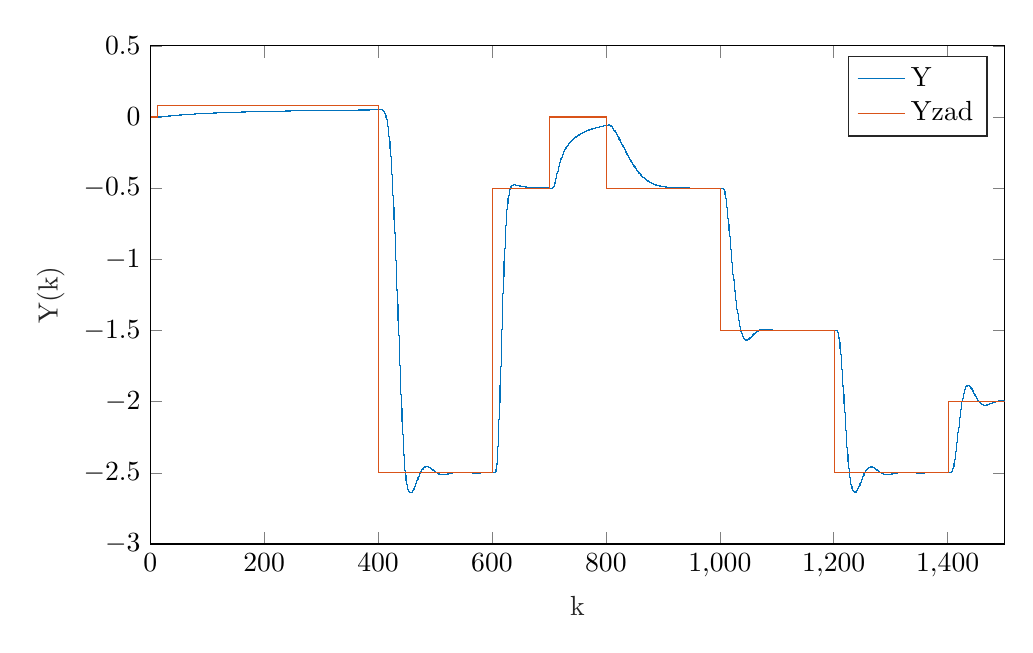
\begin{tikzpicture}

\begin{axis}[%
width=4.272in,
height=2.491in,
at={(0.717in,0.423in)},
scale only axis,
xmin=0,
xmax=1500,
xlabel style={font=\color{white!15!black}},
xlabel={k},
ymin=-3,
ymax=0.5,
ylabel style={font=\color{white!15!black}},
ylabel={Y(k)},
axis background/.style={fill=white},
legend style={legend cell align=left, align=left, draw=white!15!black}
]
\addplot[const plot, color=mycolor1] table[row sep=crcr] {%
1	0\\
2	0\\
3	0\\
4	0\\
5	0\\
6	0\\
7	0\\
8	0\\
9	0\\
10	0\\
11	0\\
12	0\\
13	0\\
14	0\\
15	0\\
16	0\\
17	6.49717367770994e-05\\
18	0.000253940065352812\\
19	0.000558962700699545\\
20	0.000948587917999254\\
21	0.00138989457982067\\
22	0.0018571701033009\\
23	0.00233343109643054\\
24	0.00280889507828654\\
25	0.00327871076618512\\
26	0.00374096831968078\\
27	0.00419528767216122\\
28	0.00464195132108915\\
29	0.00508143828154195\\
30	0.00551421180683673\\
31	0.00594064767128903\\
32	0.00636102922044946\\
33	0.00677556708577697\\
34	0.00718442284280921\\
35	0.00758772839122951\\
36	0.00798559917812108\\
37	0.00837814209801549\\
38	0.00876545964990992\\
39	0.00914765180878662\\
40	0.00952481667238395\\
41	0.0098970505479392\\
42	0.0102644478442843\\
43	0.0106271009419327\\
44	0.0109851001050883\\
45	0.0113385334464607\\
46	0.0116874869349335\\
47	0.012032044431487\\
48	0.0123722877408363\\
49	0.0127082966700781\\
50	0.0130401490891339\\
51	0.0133679209902804\\
52	0.0136916865456016\\
53	0.0140115181620334\\
54	0.0143274865340486\\
55	0.0146396606941673\\
56	0.0149481080614932\\
57	0.0152528944884452\\
58	0.0155540843058198\\
59	0.015851740366285\\
60	0.0161459240863873\\
61	0.0164366954871378\\
62	0.0167241132332358\\
63	0.0170082346709824\\
64	0.0172891158649345\\
65	0.0175668116333469\\
66	0.0178413755824479\\
67	0.0181128601395932\\
68	0.01838131658534\\
69	0.0186467950844819\\
70	0.0189093447160837\\
71	0.0191690135025537\\
72	0.0194258484377886\\
73	0.019679895514426\\
74	0.0199311997502371\\
75	0.0201798052136907\\
76	0.020425755048719\\
77	0.0206690914987142\\
78	0.0209098559297829\\
79	0.0211480888532863\\
80	0.0213838299476896\\
81	0.0216171180797473\\
82	0.0218479913250462\\
83	0.0220764869879295\\
84	0.0223026416208232\\
85	0.0225264910429856\\
86	0.0227480703587007\\
87	0.0229674139749331\\
88	0.0231845556184641\\
89	0.0233995283525262\\
90	0.0236123645929535\\
91	0.0238230961238629\\
92	0.0240317541128841\\
93	0.0242383691259516\\
94	0.024442971141674\\
95	0.0246455895652951\\
96	0.0248462532422587\\
97	0.0250449904713924\\
98	0.0252418290177209\\
99	0.0254367961249212\\
100	0.0256299185274325\\
101	0.0258212224622304\\
102	0.026010733680277\\
103	0.0261984774576573\\
104	0.0263844786064112\\
105	0.0265687614850714\\
106	0.0267513500089164\\
107	0.0269322676599474\\
108	0.0271115374965968\\
109	0.0272891821631789\\
110	0.0274652238990888\\
111	0.027639684547757\\
112	0.0278125855653701\\
113	0.0279839480293603\\
114	0.0281537926466753\\
115	0.0283221397618316\\
116	0.0284890093647599\\
117	0.0286544210984482\\
118	0.0288183942663883\\
119	0.0289809478398318\\
120	0.0291421004648623\\
121	0.0293018704692865\\
122	0.0294602758693533\\
123	0.0296173343763019\\
124	0.0297730634027477\\
125	0.0299274800689076\\
126	0.0300806012086713\\
127	0.0302324433755221\\
128	0.0303830228483123\\
129	0.0305323556368959\\
130	0.0306804574876248\\
131	0.0308273438887102\\
132	0.0309730300754545\\
133	0.031117531035357\\
134	0.0312608615130958\\
135	0.0314030360153921\\
136	0.0315440688157561\\
137	0.0316839739591223\\
138	0.0318227652663734\\
139	0.0319604563387584\\
140	0.0320970605622064\\
141	0.0322325911115395\\
142	0.0323670609545879\\
143	0.0325004828562085\\
144	0.0326328693822114\\
145	0.0327642329031955\\
146	0.0328945855982955\\
147	0.0330239394588446\\
148	0.0331523062919517\\
149	0.0332796977239992\\
150	0.0334061252040605\\
151	0.0335316000072409\\
152	0.0336561332379436\\
153	0.0337797358330619\\
154	0.0339024185651013\\
155	0.0340241920452313\\
156	0.0341450667262702\\
157	0.0342650529056037\\
158	0.0343841607280398\\
159	0.0345024001886009\\
160	0.0346197811352549\\
161	0.0347363132715872\\
162	0.0348520061594146\\
163	0.0349668692213428\\
164	0.0350809117432693\\
165	0.0351941428768319\\
166	0.0353065716418054\\
167	0.0354182069284473\\
168	0.0355290574997937\\
169	0.0356391319939065\\
170	0.0357484389260734\\
171	0.0358569866909617\\
172	0.0359647835647272\\
173	0.0360718377070788\\
174	0.0361781571633005\\
175	0.0362837498662314\\
176	0.036388623638205\\
177	0.0364927861929483\\
178	0.0365962451374422\\
179	0.0366990079737441\\
180	0.0368010821007729\\
181	0.036902474816058\\
182	0.0370031933174534\\
183	0.0371032447048163\\
184	0.0372026359816527\\
185	0.03730137405673\\
186	0.0373994657456569\\
187	0.0374969177724327\\
188	0.037593736770965\\
189	0.0376899292865579\\
190	0.0377855017773708\\
191	0.0378804606158489\\
192	0.0379748120901247\\
193	0.0380685624053932\\
194	0.03816171768526\\
195	0.038254283973063\\
196	0.0383462672331688\\
197	0.0384376733522443\\
198	0.0385285081405034\\
199	0.0386187773329305\\
200	0.0387084865904799\\
201	0.0387976415012526\\
202	0.0388862475816517\\
203	0.0389743102775145\\
204	0.0390618349652239\\
205	0.0391488269527996\\
206	0.0392352914809676\\
207	0.0393212337242107\\
208	0.0394066587917992\\
209	0.0394915717288018\\
210	0.039575977517079\\
211	0.0396598810762574\\
212	0.039743287264686\\
213	0.0398262008803753\\
214	0.0399086266619191\\
215	0.0399905692893999\\
216	0.0400720333852768\\
217	0.0401530235152584\\
218	0.0402335441891597\\
219	0.0403135998617427\\
220	0.0403931949335435\\
221	0.040472333751683\\
222	0.0405510206106638\\
223	0.0406292597531536\\
224	0.0407070553707532\\
225	0.0407844116047524\\
226	0.0408613325468713\\
227	0.0409378222399897\\
228	0.0410138846788629\\
229	0.0410895238108251\\
230	0.041164743536481\\
231	0.0412395477103847\\
232	0.0413139401417076\\
233	0.0413879245948938\\
234	0.0414615047903052\\
235	0.0415346844048545\\
236	0.0416074670726286\\
237	0.0416798563854999\\
238	0.0417518558937283\\
239	0.0418234691065523\\
240	0.0418946994927706\\
241	0.0419655504813136\\
242	0.0420360254618049\\
243	0.0421061277851141\\
244	0.0421758607638999\\
245	0.0422452276731438\\
246	0.042314231750676\\
247	0.0423828761976911\\
248	0.0424511641792563\\
249	0.042519098824811\\
250	0.0425866832286579\\
251	0.042653920450446\\
252	0.042720813515646\\
253	0.0427873654160177\\
254	0.0428535791100701\\
255	0.0429194575235132\\
256	0.0429850035497035\\
257	0.0430502200500814\\
258	0.0431151098546023\\
259	0.0431796757621603\\
260	0.0432439205410049\\
261	0.0433078469291517\\
262	0.0433714576347861\\
263	0.0434347553366602\\
264	0.0434977426844846\\
265	0.0435604222993123\\
266	0.0436227967739185\\
267	0.0436848686731722\\
268	0.043746640534404\\
269	0.043808114867767\\
270	0.0438692941565922\\
271	0.0439301808577383\\
272	0.0439907774019367\\
273	0.0440510861941303\\
274	0.0441111096138075\\
275	0.0441708500153309\\
276	0.044230309728261\\
277	0.0442894910576752\\
278	0.0443483962844813\\
279	0.0444070276657265\\
280	0.0444653874349021\\
281	0.0445234778022429\\
282	0.0445813009550223\\
283	0.0446388590578432\\
284	0.0446961542529243\\
285	0.0447531886603818\\
286	0.0448099643785075\\
287	0.0448664834840421\\
288	0.0449227480324449\\
289	0.0449787600581592\\
290	0.0450345215748739\\
291	0.045090034575781\\
292	0.0451453010338296\\
293	0.0452003229019758\\
294	0.0452551021134294\\
295	0.0453096405818965\\
296	0.0453639402018186\\
297	0.0454180028486087\\
298	0.0454718303788833\\
299	0.0455254246306913\\
300	0.0455787874237399\\
301	0.0456319205596166\\
302	0.0456848258220084\\
303	0.0457375049769178\\
304	0.0457899597728758\\
305	0.0458421919411514\\
306	0.0458942031959585\\
307	0.04594599523466\\
308	0.0459975697379682\\
309	0.0460489283701436\\
310	0.0461000727791896\\
311	0.0461510045970452\\
312	0.0462017254397749\\
313	0.0462522369077557\\
314	0.0463025405858618\\
315	0.0463526380436462\\
316	0.0464025308355205\\
317	0.0464522205009312\\
318	0.0465017085645348\\
319	0.0465509965363693\\
320	0.0466000859120239\\
321	0.0466489781728064\\
322	0.0466976747859083\\
323	0.0467461772045671\\
324	0.0467944868682268\\
325	0.0468426052026967\\
326	0.0468905336203069\\
327	0.0469382735200626\\
328	0.0469858262877958\\
329	0.0470331932963155\\
330	0.0470803759055548\\
331	0.0471273754627175\\
332	0.0471741933024214\\
333	0.0472208307468404\\
334	0.0472672891058443\\
335	0.0473135696771374\\
336	0.0473596737463942\\
337	0.0474056025873942\\
338	0.0474513574621545\\
339	0.0474969396210607\\
340	0.0475423503029963\\
341	0.0475875907354698\\
342	0.0476326621347405\\
343	0.0476775657059433\\
344	0.0477223026432103\\
345	0.0477668741297923\\
346	0.0478112813381781\\
347	0.0478555254302119\\
348	0.0478996075572099\\
349	0.0479435288600751\\
350	0.0479872904694102\\
351	0.0480308935056294\\
352	0.0480743390790693\\
353	0.0481176282900971\\
354	0.0481607622292186\\
355	0.0482037419771841\\
356	0.0482465686050934\\
357	0.048289243174499\\
358	0.0483317667375086\\
359	0.0483741403368853\\
360	0.0484163650061481\\
361	0.0484584417696693\\
362	0.048500371642772\\
363	0.048542155631826\\
364	0.0485837947343421\\
365	0.0486252899390659\\
366	0.0486666422260699\\
367	0.0487078525668445\\
368	0.0487489219243883\\
369	0.0487898512532968\\
370	0.0488306414998499\\
371	0.0488712936020992\\
372	0.048911808489953\\
373	0.0489521870852611\\
374	0.0489924303018983\\
375	0.0490325390458471\\
376	0.0490725142152786\\
377	0.0491123567006335\\
378	0.0491520673847014\\
379	0.0491916471426993\\
380	0.0492310968423493\\
381	0.049270417343955\\
382	0.0493096095004773\\
383	0.0493486741576093\\
384	0.04938761215385\\
385	0.0494264243205775\\
386	0.0494651114821208\\
387	0.0495036744558315\\
388	0.0495421140521535\\
389	0.0495804310746935\\
390	0.0496186263202887\\
391	0.0496567005790757\\
392	0.0496946546345568\\
393	0.0497324892636667\\
394	0.049770205236838\\
395	0.0498078033180658\\
396	0.049845284264972\\
397	0.049882648828868\\
398	0.0499198977548179\\
399	0.0499570317816994\\
400	0.0499940516422658\\
401	0.0500309580632055\\
402	0.0500677517652021\\
403	0.0501044334629932\\
404	0.0501410038654286\\
405	0.0501774636755281\\
406	0.0501732976612908\\
407	0.0490041366763184\\
408	0.0465289628914037\\
409	0.0427579051954193\\
410	0.0376105133691585\\
411	0.0308706677318635\\
412	0.0221990241604669\\
413	0.0111600535345114\\
414	-0.00274900485623176\\
415	-0.0200694135856798\\
416	-0.0413522756193917\\
417	-0.0671302287532631\\
418	-0.0978906622219282\\
419	-0.134052124191253\\
420	-0.175945539494681\\
421	-0.223801357265741\\
422	-0.277743005547366\\
423	-0.337786275156232\\
424	-0.403843645211453\\
425	-0.475732203610437\\
426	-0.553183726393474\\
427	-0.635855614926891\\
428	-0.723341672929035\\
429	-0.815182052805617\\
430	-0.910872040840749\\
431	-1.00986963417384\\
432	-1.11160206422284\\
433	-1.21547153703534\\
434	-1.32086050104577\\
435	-1.42713673466942\\
436	-1.53365849008766\\
437	-1.6397798539946\\
438	-1.74485640599204\\
439	-1.84825118150952\\
440	-1.94934088528562\\
441	-2.04752225679798\\
442	-2.14147639133622\\
443	-2.22848705208996\\
444	-2.30650641169099\\
445	-2.37465598541462\\
446	-2.43286660292565\\
447	-2.4816016550143\\
448	-2.52164893664436\\
449	-2.55396798108606\\
450	-2.5795814790502\\
451	-2.59950107109505\\
452	-2.61467940609752\\
453	-2.62590828629046\\
454	-2.63378089060945\\
455	-2.63874178924967\\
456	-2.64114062932128\\
457	-2.64126817461759\\
458	-2.63937948418553\\
459	-2.63570825251314\\
460	-2.63047528077431\\
461	-2.62389310229332\\
462	-2.61616811570904\\
463	-2.60750113232639\\
464	-2.59808694772942\\
465	-2.5881133508886\\
466	-2.57775985228968\\
467	-2.56719632341376\\
468	-2.55658167850336\\
469	-2.54606268644621\\
470	-2.53577296966093\\
471	-2.52583222413818\\
472	-2.51634567775718\\
473	-2.5074037910575\\
474	-2.49908219477772\\
475	-2.49144185101525\\
476	-2.4845294193741\\
477	-2.47837780563445\\
478	-2.47300686805388\\
479	-2.4684242551845\\
480	-2.46462634887147\\
481	-2.46159928670369\\
482	-2.45932003944417\\
483	-2.45775752071177\\
484	-2.45687370826885\\
485	-2.45662475855627\\
486	-2.45696209849492\\
487	-2.45783348094646\\
488	-2.45918399252134\\
489	-2.46095700458573\\
490	-2.46309506031375\\
491	-2.46554069243592\\
492	-2.46823716794215\\
493	-2.47112915740838\\
494	-2.47416332784024\\
495	-2.47728885897917\\
496	-2.48045788391343\\
497	-2.48362585559632\\
498	-2.486751841516\\
499	-2.4897987493012\\
500	-2.4927334865011\\
501	-2.49552705815814\\
502	-2.49815460610983\\
503	-2.50059539421866\\
504	-2.50283274394297\\
505	-2.5048539248312\\
506	-2.50665000464879\\
507	-2.50821566393326\\
508	-2.50954897981829\\
509	-2.51065118397231\\
510	-2.51152639946038\\
511	-2.51218136126005\\
512	-2.51262512504241\\
513	-2.51286876866903\\
514	-2.51292509065536\\
515	-2.51280830961386\\
516	-2.51253376841701\\
517	-2.51211764651742\\
518	-2.51157668353076\\
519	-2.5109279168352\\
520	-2.51018843557133\\
521	-2.50937515304648\\
522	-2.50850459916253\\
523	-2.50759273410219\\
524	-2.50665478413193\\
525	-2.50570510001539\\
526	-2.50475703818392\\
527	-2.50382286448644\\
528	-2.50291368004173\\
529	-2.50203936844631\\
530	-2.50120856335293\\
531	-2.50042863522897\\
532	-2.49970569593257\\
533	-2.49904461960657\\
534	-2.49844907828611\\
535	-2.49792159054349\\
536	-2.49746358145265\\
537	-2.49707545214243\\
538	-2.49675665722116\\
539	-2.49650578839157\\
540	-2.49632066263271\\
541	-2.49619841340055\\
542	-2.49613558338942\\
543	-2.49612821749901\\
544	-2.49617195476358\\
545	-2.49626211811931\\
546	-2.49639380100916\\
547	-2.49656194995103\\
548	-2.49676144232143\\
549	-2.49698715873237\\
550	-2.49723404950154\\
551	-2.4974971948345\\
552	-2.49777185845027\\
553	-2.49805353448899\\
554	-2.4983379876398\\
555	-2.4986212865193\\
556	-2.49889983041522\\
557	-2.49917036958535\\
558	-2.49943001936896\\
559	-2.4996762684262\\
560	-2.49990698147065\\
561	-2.50012039690131\\
562	-2.50031511977294\\
563	-2.50049011056836\\
564	-2.50064467025313\\
565	-2.50077842210242\\
566	-2.50089129079273\\
567	-2.50098347924685\\
568	-2.50105544371112\\
569	-2.5011078675288\\
570	-2.50114163405358\\
571	-2.50115779912334\\
572	-2.50115756348695\\
573	-2.50114224554634\\
574	-2.5011132547435\\
575	-2.50107206588771\\
576	-2.5010201946826\\
577	-2.50095917467669\\
578	-2.5008905358245\\
579	-2.50081578480986\\
580	-2.50073638724762\\
581	-2.50065375184641\\
582	-2.50056921658272\\
583	-2.50048403690633\\
584	-2.50039937596885\\
585	-2.50031629684113\\
586	-2.50023575666223\\
587	-2.50015860264164\\
588	-2.50008556981841\\
589	-2.50001728046572\\
590	-2.49995424501648\\
591	-2.49989686437575\\
592	-2.49984543347846\\
593	-2.49980014594564\\
594	-2.4997610996901\\
595	-2.49972830332189\\
596	-2.49970168320545\\
597	-2.49968109102387\\
598	-2.49966631171051\\
599	-2.49965707161484\\
600	-2.49965304677707\\
601	-2.49965387119457\\
602	-2.49965914497295\\
603	-2.49966844226463\\
604	-2.4996813189083\\
605	-2.49969731969378\\
606	-2.49315940731296\\
607	-2.47381471475503\\
608	-2.43813887530138\\
609	-2.38466913571464\\
610	-2.31346242037545\\
611	-2.22568007519594\\
612	-2.1232820257921\\
613	-2.00879641558732\\
614	-1.88513409987954\\
615	-1.75542679934013\\
616	-1.62287658937541\\
617	-1.49061172677289\\
618	-1.36154978103588\\
619	-1.23827365028951\\
620	-1.12292890658948\\
621	-1.01715148712842\\
622	-0.922032763955286\\
623	-0.838124841480951\\
624	-0.765483624002902\\
625	-0.70374217470195\\
626	-0.652203445928138\\
627	-0.609940306284873\\
628	-0.575891880287022\\
629	-0.548947909103803\\
630	-0.528016229241756\\
631	-0.512071714835278\\
632	-0.500187584219464\\
633	-0.491551609497909\\
634	-0.485470531283688\\
635	-0.481366064783745\\
636	-0.478765530517634\\
637	-0.477289572684918\\
638	-0.47663880380018\\
639	-0.476580637582018\\
640	-0.476937093787581\\
641	-0.477573993313054\\
642	-0.478391702551387\\
643	-0.479317415497298\\
644	-0.480298860201921\\
645	-0.48129926384894\\
646	-0.482293391962981\\
647	-0.483264479671867\\
648	-0.484201887490912\\
649	-0.485099334552012\\
650	-0.485953584511079\\
651	-0.486763481075902\\
652	-0.48752924985392\\
653	-0.488252000413441\\
654	-0.488933376932965\\
655	-0.489575317702902\\
656	-0.490179893305125\\
657	-0.490749200849986\\
658	-0.491285297527101\\
659	-0.49179016123394\\
660	-0.492265669458793\\
661	-0.492713590145542\\
662	-0.49313558015081\\
663	-0.493533188276624\\
664	-0.493907860848942\\
665	-0.494260948512411\\
666	-0.494593713400164\\
667	-0.494907336172187\\
668	-0.4952029226402\\
669	-0.495481509843356\\
670	-0.49574407153121\\
671	-0.495991523065421\\
672	-0.496224725781973\\
673	-0.496444490869888\\
674	-0.496651582826613\\
675	-0.496846722548472\\
676	-0.497030590109606\\
677	-0.497203827276401\\
678	-0.497367039797594\\
679	-0.497520799503775\\
680	-0.497665646244064\\
681	-0.49780208968269\\
682	-0.497930610973817\\
683	-0.498051664329413\\
684	-0.498165678492071\\
685	-0.498273058122374\\
686	-0.498374185108542\\
687	-0.498469419804742\\
688	-0.498559102203282\\
689	-0.498643553045111\\
690	-0.498723074872398\\
691	-0.498797953026458\\
692	-0.498868456593967\\
693	-0.498934839304075\\
694	-0.498997340378864\\
695	-0.499056185339372\\
696	-0.499111586769331\\
697	-0.499163745038595\\
698	-0.499212848988194\\
699	-0.499259076578831\\
700	-0.499302595504572\\
701	-0.499343563773435\\
702	-0.499382130256474\\
703	-0.49941843520694\\
704	-0.49945261075099\\
705	-0.4994847813514\\
706	-0.498031379176469\\
707	-0.493916172808089\\
708	-0.486751558724918\\
709	-0.476661323696111\\
710	-0.464063364712556\\
711	-0.449513195142597\\
712	-0.433599814931928\\
713	-0.416880998980061\\
714	-0.399846523359255\\
715	-0.382900695709526\\
716	-0.366357940124519\\
717	-0.35044689486199\\
718	-0.335319679326723\\
719	-0.321063857774868\\
720	-0.307715296993935\\
721	-0.295270654532712\\
722	-0.283698676800524\\
723	-0.272949843438105\\
724	-0.26296417494982\\
725	-0.253677225933434\\
726	-0.245024423292868\\
727	-0.236943987711109\\
728	-0.229378709052164\\
729	-0.222276844587429\\
730	-0.215592384645386\\
731	-0.209284893440778\\
732	-0.203319091254941\\
733	-0.19766430335356\\
734	-0.192293864520879\\
735	-0.187184537649351\\
736	-0.182315980979098\\
737	-0.177670281014635\\
738	-0.173231556045405\\
739	-0.168985627530008\\
740	-0.164919752311097\\
741	-0.161022406739906\\
742	-0.157283113492417\\
743	-0.153692302515256\\
744	-0.150241198680853\\
745	-0.146921730038697\\
746	-0.143726451822843\\
747	-0.140648482505113\\
748	-0.137681449121917\\
749	-0.134819439843852\\
750	-0.132056962318628\\
751	-0.1293889067278\\
752	-0.126810512787687\\
753	-0.124317340124509\\
754	-0.121905241588444\\
755	-0.119570339161236\\
756	-0.117309002172379\\
757	-0.115117827580539\\
758	-0.112993622107079\\
759	-0.110933386032015\\
760	-0.108934298482222\\
761	-0.106993704058797\\
762	-0.105109100666016\\
763	-0.103278128418549\\
764	-0.101498559516711\\
765	-0.0997682889914783\\
766	-0.0980853262319186\\
767	-0.0964477872173741\\
768	-0.0948538873854905\\
769	-0.0933019350748528\\
770	-0.0917903254877866\\
771	-0.0903175351248422\\
772	-0.0888821166477118\\
773	-0.0874826941319203\\
774	-0.0861179586746612\\
775	-0.0847866643267033\\
776	-0.0834876243204208\\
777	-0.0822197075687717\\
778	-0.0809818354125045\\
779	-0.0797729785950553\\
780	-0.0785921544465427\\
781	-0.077438424260005\\
782	-0.0763108908445765\\
783	-0.0752086962416922\\
784	-0.07413101959166\\
785	-0.0730770751390622\\
786	-0.0720461103664605\\
787	-0.0710374042467893\\
788	-0.070050265605645\\
789	-0.0690840315854248\\
790	-0.0681380662039375\\
791	-0.0672117590007231\\
792	-0.0663045237648673\\
793	-0.0654157973386022\\
794	-0.0645450384914381\\
795	-0.0636917268599905\\
796	-0.0628553619490405\\
797	-0.0620354621897169\\
798	-0.0612315640509994\\
799	-0.0604432212010338\\
800	-0.0596700037150105\\
801	-0.0589114973266021\\
802	-0.0581673027201745\\
803	-0.0574370348611901\\
804	-0.0567203223624083\\
805	-0.0560168068836585\\
806	-0.0560513991696216\\
807	-0.0573847077802722\\
808	-0.0600489397650563\\
809	-0.063845184055828\\
810	-0.0685134535647832\\
811	-0.073815806061501\\
812	-0.0795664050146557\\
813	-0.0856338565851602\\
814	-0.0919319444222781\\
815	-0.0984074816431728\\
816	-0.105029274797346\\
817	-0.11177956372289\\
818	-0.118648015942985\\
819	-0.125627838843531\\
820	-0.132713452348614\\
821	-0.139899219406076\\
822	-0.147178843682106\\
823	-0.154545159406615\\
824	-0.161990132338364\\
825	-0.169504960469327\\
826	-0.177080210952727\\
827	-0.184705960245272\\
828	-0.192371922657926\\
829	-0.200067562573782\\
830	-0.207782190598335\\
831	-0.215505045971912\\
832	-0.223225368060179\\
833	-0.230932459474096\\
834	-0.238615742825926\\
835	-0.246264812547708\\
836	-0.253869482694385\\
837	-0.261419831262397\\
838	-0.268906241275595\\
839	-0.276319438707252\\
840	-0.283650527198379\\
841	-0.290891019478622\\
842	-0.2980328653796\\
843	-0.305068476338958\\
844	-0.311990746316788\\
845	-0.318793069078052\\
846	-0.325469351830361\\
847	-0.332014025243183\\
848	-0.338422049910171\\
849	-0.344688919349786\\
850	-0.350810659669898\\
851	-0.356783826049304\\
852	-0.3626054962128\\
853	-0.368273261096602\\
854	-0.373785212917445\\
855	-0.379139930871724\\
856	-0.384336464700644\\
857	-0.389374316363667\\
858	-0.394253420065755\\
859	-0.398974120884122\\
860	-0.403537152237791\\
861	-0.407943612438228\\
862	-0.412194940552089\\
863	-0.416292891797886\\
864	-0.420239512687337\\
865	-0.424037116109703\\
866	-0.427688256543694\\
867	-0.43119570556687\\
868	-0.4345624278171\\
869	-0.437791557544836\\
870	-0.440886375878914\\
871	-0.443850288912584\\
872	-0.446686806700613\\
873	-0.449399523242869\\
874	-0.451992097514865\\
875	-0.454468235591489\\
876	-0.456831673896711\\
877	-0.459086163599476\\
878	-0.461235456164359\\
879	-0.463283290054961\\
880	-0.465233378578466\\
881	-0.467089398851209\\
882	-0.468854981857676\\
883	-0.470533703568906\\
884	-0.472129077080794\\
885	-0.473644545728356\\
886	-0.475083477128429\\
887	-0.476449158100555\\
888	-0.477744790413891\\
889	-0.47897348730678\\
890	-0.480138270725073\\
891	-0.481242069225321\\
892	-0.482287716489549\\
893	-0.483277950399283\\
894	-0.484215412617925\\
895	-0.485102648632273\\
896	-0.485942108205931\\
897	-0.486736146199577\\
898	-0.487487023715333\\
899	-0.48819690952499\\
900	-0.488867881744284\\
901	-0.489501929718032\\
902	-0.490100956083444\\
903	-0.490666778981444\\
904	-0.491201134388345\\
905	-0.491705678542567\\
906	-0.492181990443452\\
907	-0.492631574401412\\
908	-0.493055862620775\\
909	-0.493456217798679\\
910	-0.493833935725244\\
911	-0.494190247872002\\
912	-0.494526323957203\\
913	-0.494843274478116\\
914	-0.495142153201845\\
915	-0.495423959607458\\
916	-0.495689641273375\\
917	-0.495940096205042\\
918	-0.496176175098859\\
919	-0.496398683539196\\
920	-0.496608384126097\\
921	-0.496805998531969\\
922	-0.496992209486146\\
923	-0.497167662686774\\
924	-0.497332968639902\\
925	-0.497488704426099\\
926	-0.497635415395267\\
927	-0.497773616790587\\
928	-0.497903795302843\\
929	-0.498026410556533\\
930	-0.498141896529382\\
931	-0.498250662907004\\
932	-0.498353096374568\\
933	-0.498449561847427\\
934	-0.498540403642702\\
935	-0.498625946593888\\
936	-0.498706497110556\\
937	-0.498782344185227\\
938	-0.498853760349522\\
939	-0.498921002581622\\
940	-0.498984313167119\\
941	-0.499043920515232\\
942	-0.499100039932371\\
943	-0.499152874354973\\
944	-0.499202615043477\\
945	-0.499249442239256\\
946	-0.499293525786267\\
947	-0.499335025719125\\
948	-0.499374092819245\\
949	-0.499410869140626\\
950	-0.499445488506816\\
951	-0.499478076980492\\
952	-0.499508753307094\\
953	-0.499537629333816\\
954	-0.499564810405263\\
955	-0.499590395736992\\
956	-0.499614478768108\\
957	-0.499637147494025\\
958	-0.499658484780466\\
959	-0.49967856865971\\
960	-0.499697472610042\\
961	-0.499715265819337\\
962	-0.499732013433626\\
963	-0.499747776791493\\
964	-0.49976261364507\\
965	-0.499776578368382\\
966	-0.499789722153736\\
967	-0.499802093196842\\
968	-0.499813736871274\\
969	-0.499824695892886\\
970	-0.499835010474742\\
971	-0.499844718473106\\
972	-0.49985385552498\\
973	-0.499862455177693\\
974	-0.499870549010975\\
975	-0.499878166751954\\
976	-0.49988533638348\\
977	-0.49989208424615\\
978	-0.499898435134412\\
979	-0.499904412387066\\
980	-0.499910037972506\\
981	-0.499915332568988\\
982	-0.499920315640222\\
983	-0.499925005506559\\
984	-0.499929419412013\\
985	-0.499933573587381\\
986	-0.499937483309665\\
987	-0.499941162958032\\
988	-0.499944626066491\\
989	-0.499947885373498\\
990	-0.49995095286865\\
991	-0.499953839836654\\
992	-0.499956556898715\\
993	-0.499959114051501\\
994	-0.499961520703826\\
995	-0.499963785711183\\
996	-0.499965917408255\\
997	-0.499967923639511\\
998	-0.499969811788019\\
999	-0.499971588802559\\
1000	-0.499973261223151\\
1001	-0.499974835205083\\
1002	-0.499976316541526\\
1003	-0.499977710684827\\
1004	-0.499979022766546\\
1005	-0.499980257616319\\
1006	-0.502888298409256\\
1007	-0.510992599036443\\
1008	-0.525124342108412\\
1009	-0.545238977652221\\
1010	-0.570822404327137\\
1011	-0.601151360912943\\
1012	-0.635445522791986\\
1013	-0.672948237913594\\
1014	-0.712963927051411\\
1015	-0.754870834990951\\
1016	-0.798120799691724\\
1017	-0.842232980290172\\
1018	-0.886785469661219\\
1019	-0.931406866176476\\
1020	-0.975768783704786\\
1021	-1.01957965791747\\
1022	-1.06257987437869\\
1023	-1.10453808615474\\
1024	-1.14524852349691\\
1025	-1.18452908629854\\
1026	-1.22222002481742\\
1027	-1.25818303956504\\
1028	-1.29230065933196\\
1029	-1.32447578310104\\
1030	-1.35463129543696\\
1031	-1.38270968538784\\
1032	-1.40867261614843\\
1033	-1.43250040711807\\
1034	-1.45419140200877\\
1035	-1.47376120675337\\
1036	-1.4912417894978\\
1037	-1.50668044221725\\
1038	-1.52013860967942\\
1039	-1.53169059672792\\
1040	-1.54142216925877\\
1041	-1.54942906785846\\
1042	-1.55581545587973\\
1043	-1.56069232575422\\
1044	-1.56417588857803\\
1045	-1.56638597245931\\
1046	-1.56744445480359\\
1047	-1.56747375266342\\
1048	-1.5665953935494\\
1049	-1.56492868676433\\
1050	-1.56258951247689\\
1051	-1.55968924251001\\
1052	-1.55633380330776\\
1053	-1.5526228878965\\
1054	-1.54864932000591\\
1055	-1.54449856998967\\
1056	-1.54024841890092\\
1057	-1.535968764131\\
1058	-1.53172155748842\\
1059	-1.52756086453098\\
1060	-1.5235330323964\\
1061	-1.51967695230884\\
1062	-1.51602440235537\\
1063	-1.51260045599136\\
1064	-1.50942394199795\\
1065	-1.50650794221958\\
1066	-1.50386031428949\\
1067	-1.50148422763995\\
1068	-1.49937870232723\\
1069	-1.49753914151866\\
1070	-1.49595784983687\\
1071	-1.4946245310899\\
1072	-1.49352676019704\\
1073	-1.49265042532192\\
1074	-1.49198013732572\\
1075	-1.49149960464182\\
1076	-1.49119197254262\\
1077	-1.49104012651863\\
1078	-1.4910269601221\\
1079	-1.49113560814948\\
1080	-1.4913496464569\\
1081	-1.49165326002993\\
1082	-1.49203138117529\\
1083	-1.49246979987582\\
1084	-1.49295524846347\\
1085	-1.49347546282626\\
1086	-1.49401922238314\\
1087	-1.4945763710434\\
1088	-1.49513782132153\\
1089	-1.49569554370925\\
1090	-1.49624254332035\\
1091	-1.49677282572355\\
1092	-1.49728135376878\\
1093	-1.49776399709473\\
1094	-1.49821747588398\\
1095	-1.49863930030732\\
1096	-1.49902770697343\\
1097	-1.49938159357522\\
1098	-1.49970045280067\\
1099	-1.49998430645511\\
1100	-1.5002336406251\\
1101	-1.50044934260061\\
1102	-1.50063264016432\\
1103	-1.50078504375416\\
1104	-1.50090829190831\\
1105	-1.50100430031138\\
1106	-1.50107511467634\\
1107	-1.50112286761973\\
1108	-1.50114973961723\\
1109	-1.50115792406324\\
1110	-1.50114959640206\\
1111	-1.50112688724852\\
1112	-1.50109185937346\\
1113	-1.50104648839322\\
1114	-1.50099264697251\\
1115	-1.50093209232633\\
1116	-1.50086645678817\\
1117	-1.50079724119887\\
1118	-1.50072581086245\\
1119	-1.50065339381115\\
1120	-1.50058108112221\\
1121	-1.50050982903258\\
1122	-1.50044046260396\\
1123	-1.50037368070012\\
1124	-1.50031006204942\\
1125	-1.50025007217861\\
1126	-1.50019407101816\\
1127	-1.50014232099477\\
1128	-1.50009499544274\\
1129	-1.5000521871818\\
1130	-1.50001391712597\\
1131	-1.4999801428036\\
1132	-1.49995076668509\\
1133	-1.49992564422975\\
1134	-1.49990459157812\\
1135	-1.49988739282992\\
1136	-1.49987380686039\\
1137	-1.49986357364028\\
1138	-1.49985642003536\\
1139	-1.49985206507141\\
1140	-1.4998502246595\\
1141	-1.49985061578444\\
1142	-1.49985296016584\\
1143	-1.49985698740742\\
1144	-1.49986243765508\\
1145	-1.49986906378817\\
1146	-1.49987663317193\\
1147	-1.49988492900121\\
1148	-1.49989375126772\\
1149	-1.49990291738379\\
1150	-1.49991226249645\\
1151	-1.4999216395255\\
1152	-1.4999309189589\\
1153	-1.49993998843787\\
1154	-1.49994875216305\\
1155	-1.49995713015151\\
1156	-1.49996505737287\\
1157	-1.49997248279091\\
1158	-1.49997936833499\\
1159	-1.49998568782364\\
1160	-1.49999142586073\\
1161	-1.49999657672211\\
1162	-1.50000114324905\\
1163	-1.50000513576227\\
1164	-1.50000857100866\\
1165	-1.50001147115078\\
1166	-1.50001386280753\\
1167	-1.50001577615234\\
1168	-1.50001724407422\\
1169	-1.50001830140494\\
1170	-1.50001898421488\\
1171	-1.50001932917823\\
1172	-1.50001937300798\\
1173	-1.50001915195933\\
1174	-1.50001870140005\\
1175	-1.50001805544533\\
1176	-1.50001724665398\\
1177	-1.50001630578276\\
1178	-1.50001526159478\\
1179	-1.50001414071814\\
1180	-1.50001296755044\\
1181	-1.5000117642048\\
1182	-1.50001055049319\\
1183	-1.5000093439425\\
1184	-1.50000815983938\\
1185	-1.50000701129948\\
1186	-1.50000590935742\\
1187	-1.50000486307355\\
1188	-1.50000387965413\\
1189	-1.50000296458162\\
1190	-1.50000212175216\\
1191	-1.50000135361746\\
1192	-1.50000066132864\\
1193	-1.50000004488\\
1194	-1.49999950325055\\
1195	-1.49999903454198\\
1196	-1.49999863611138\\
1197	-1.49999830469776\\
1198	-1.49999803654136\\
1199	-1.49999782749502\\
1200	-1.49999767312716\\
1201	-1.49999756881592\\
1202	-1.49999750983436\\
1203	-1.49999749142664\\
1204	-1.49999750887528\\
1205	-1.49999755755962\\
1206	-1.50318470104766\\
1207	-1.51233754567738\\
1208	-1.52880605521435\\
1209	-1.55297937366037\\
1210	-1.58463710648942\\
1211	-1.62319620295221\\
1212	-1.66787404035895\\
1213	-1.71779220733169\\
1214	-1.77204089836207\\
1215	-1.82971787271207\\
1216	-1.889951286298\\
1217	-1.95191249713699\\
1218	-2.01482280134492\\
1219	-2.07795663489928\\
1220	-2.14064283418116\\
1221	-2.20226492558387\\
1222	-2.26226100507418\\
1223	-2.32012350760488\\
1224	-2.37433198131072\\
1225	-2.4234463528655\\
1226	-2.46671755763316\\
1227	-2.5039549690876\\
1228	-2.53534274774247\\
1229	-2.56130061571426\\
1230	-2.58238079538934\\
1231	-2.59919386129005\\
1232	-2.61234074521156\\
1233	-2.62229730980997\\
1234	-2.62942277155835\\
1235	-2.63400266225795\\
1236	-2.63627834890015\\
1237	-2.63646617778953\\
1238	-2.6347692229527\\
1239	-2.63138406559462\\
1240	-2.62650430301408\\
1241	-2.62032192883043\\
1242	-2.61302735199905\\
1243	-2.60480857337653\\
1244	-2.5958498736963\\
1245	-2.58633025674637\\
1246	-2.57642181709383\\
1247	-2.56628815038633\\
1248	-2.55608288802289\\
1249	-2.5459484116552\\
1250	-2.53601478326235\\
1251	-2.52639891135713\\
1252	-2.5172039619346\\
1253	-2.50851901326498\\
1254	-2.50041894607128\\
1255	-2.49296455471131\\
1256	-2.48620286049721\\
1257	-2.48016760508016\\
1258	-2.47487989976631\\
1259	-2.47034900558195\\
1260	-2.46657321873486\\
1261	-2.46354083668416\\
1262	-2.46123118119176\\
1263	-2.45961565634379\\
1264	-2.45865882146948\\
1265	-2.45831946102609\\
1266	-2.45855163575819\\
1267	-2.45930570168736\\
1268	-2.46052928567621\\
1269	-2.46216820838378\\
1270	-2.4641673473527\\
1271	-2.46647143471877\\
1272	-2.46902578560186\\
1273	-2.47177695462221\\
1274	-2.47467331919542\\
1275	-2.47766558930491\\
1276	-2.48070724434731\\
1277	-2.48375489841053\\
1278	-2.48676859599261\\
1279	-2.4897120407183\\
1280	-2.49255276007275\\
1281	-2.49526220956082\\
1282	-2.49781582002638\\
1283	-2.50019299213567\\
1284	-2.50237704224969\\
1285	-2.50435510408555\\
1286	-2.50611799069916\\
1287	-2.50766002141294\\
1288	-2.50897881836266\\
1289	-2.51007507734775\\
1290	-2.51095231763883\\
1291	-2.51161661532514\\
1292	-2.51207632467289\\
1293	-2.51234179181428\\
1294	-2.51242506489714\\
1295	-2.51233960459897\\
1296	-2.51209999864919\\
1297	-2.51172168371326\\
1298	-2.51122067767572\\
1299	-2.51061332502159\\
1300	-2.50991605766122\\
1301	-2.50914517317854\\
1302	-2.50831663211293\\
1303	-2.50744587551498\\
1304	-2.50654766365326\\
1305	-2.50563593639726\\
1306	-2.50472369546613\\
1307	-2.50382290841779\\
1308	-2.5029444339627\\
1309	-2.50209796792357\\
1310	-2.50129200892886\\
1311	-2.50053384272652\\
1312	-2.4998295438346\\
1313	-2.49918399310841\\
1314	-2.49860090969908\\
1315	-2.49808289580411\\
1316	-2.49763149256628\\
1317	-2.49724724546034\\
1318	-2.49692977751545\\
1319	-2.49667786875282\\
1320	-2.49648954026973\\
1321	-2.49636214147047\\
1322	-2.49629243902883\\
1323	-2.49627670626346\\
1324	-2.49631081171298\\
1325	-2.49639030581124\\
1326	-2.49651050468097\\
1327	-2.49666657018483\\
1328	-2.49685358549439\\
1329	-2.49706662555827\\
1330	-2.49730082196896\\
1331	-2.49755142184211\\
1332	-2.49781384043204\\
1333	-2.4980837073105\\
1334	-2.49835690603349\\
1335	-2.49862960731028\\
1336	-2.49889829577138\\
1337	-2.49915979050638\\
1338	-2.49941125960825\\
1339	-2.49965022901853\\
1340	-2.49987458601698\\
1341	-2.50008257773995\\
1342	-2.50027280514501\\
1343	-2.50044421286387\\
1344	-2.50059607540339\\
1345	-2.50072798016471\\
1346	-2.50083980775391\\
1347	-2.50093171005514\\
1348	-2.50100408652857\\
1349	-2.5010575591818\\
1350	-2.50109294664516\\
1351	-2.5011112377589\\
1352	-2.50111356505433\\
1353	-2.50110117848216\\
1354	-2.50107541971044\\
1355	-2.50103769728123\\
1356	-2.50098946288151\\
1357	-2.5009321889488\\
1358	-2.5008673477974\\
1359	-2.50079639241622\\
1360	-2.50072073905573\\
1361	-2.50064175168855\\
1362	-2.50056072839708\\
1363	-2.50047888971212\\
1364	-2.50039736889873\\
1365	-2.50031720416076\\
1366	-2.50023933271216\\
1367	-2.50016458664307\\
1368	-2.50009369049105\\
1369	-2.50002726041216\\
1370	-2.49996580483465\\
1371	-2.49990972646739\\
1372	-2.49985932552824\\
1373	-2.49981480405188\\
1374	-2.49977627113416\\
1375	-2.49974374896905\\
1376	-2.49971717953558\\
1377	-2.49969643179502\\
1378	-2.49968130926333\\
1379	-2.49967155782959\\
1380	-2.4996668736987\\
1381	-2.49966691134436\\
1382	-2.49967129136798\\
1383	-2.49967960816812\\
1384	-2.49969143733593\\
1385	-2.4997063427019\\
1386	-2.49972388297005\\
1387	-2.49974361788629\\
1388	-2.49976511389773\\
1389	-2.49978794927031\\
1390	-2.49981171864125\\
1391	-2.49983603699258\\
1392	-2.4998605430404\\
1393	-2.49988490204247\\
1394	-2.49990880803449\\
1395	-2.49993198551149\\
1396	-2.49995419057721\\
1397	-2.49997521158899\\
1398	-2.49999486933042\\
1399	-2.50001301674717\\
1400	-2.50002953828473\\
1401	-2.50004434886842\\
1402	-2.50005739256779\\
1403	-2.50006864098805\\
1404	-2.50007809143144\\
1405	-2.50008576487094\\
1406	-2.49847822712883\\
1407	-2.49375015001013\\
1408	-2.48507961880764\\
1409	-2.47213901005035\\
1410	-2.45494527050297\\
1411	-2.43374823535971\\
1412	-2.40895126233537\\
1413	-2.3810552530527\\
1414	-2.35061842500333\\
1415	-2.31822655808006\\
1416	-2.28447034621745\\
1417	-2.2499277784647\\
1418	-2.21515029597507\\
1419	-2.18065197372646\\
1420	-2.14690127012839\\
1421	-2.11431504890894\\
1422	-2.0832546558375\\
1423	-2.05402385821977\\
1424	-2.02686845510209\\
1425	-2.00197735289567\\
1426	-1.97948488541669\\
1427	-1.95947414621843\\
1428	-1.94198109807362\\
1429	-1.92699923075956\\
1430	-1.91448455342524\\
1431	-1.90436073018307\\
1432	-1.89652419496644\\
1433	-1.89084911175126\\
1434	-1.88719207672544\\
1435	-1.88539648804202\\
1436	-1.88529653502254\\
1437	-1.88672078120717\\
1438	-1.88949533405878\\
1439	-1.89344660839328\\
1440	-1.89840370098708\\
1441	-1.90420040075964\\
1442	-1.91067686300048\\
1443	-1.91768097789392\\
1444	-1.92506946365985\\
1445	-1.93270871348368\\
1446	-1.94047542349124\\
1447	-1.9482570266853\\
1448	-1.9559519552722\\
1449	-1.9634697513659\\
1450	-1.97073104379549\\
1451	-1.97766740674103\\
1452	-1.98422111421838\\
1453	-1.99034480303449\\
1454	-1.99600105572288\\
1455	-2.00116191411463\\
1456	-2.00580833356229\\
1457	-2.00992958736766\\
1458	-2.01352263062413\\
1459	-2.01659143242556\\
1460	-2.01914628517637\\
1461	-2.02120309952606\\
1462	-2.0227826932152\\
1463	-2.02391008183648\\
1464	-2.02461377916536\\
1465	-2.0249251142897\\
1466	-2.02487757226111\\
1467	-2.02450616440402\\
1468	-2.0238468337559\\
1469	-2.02293590038449\\
1470	-2.0218095505483\\
1471	-2.02050337284997\\
1472	-2.01905194369698\\
1473	-2.01748846354739\\
1474	-2.01584444459865\\
1475	-2.01414944979178\\
1476	-2.01243088226628\\
1477	-2.0107138237276\\
1478	-2.00902091958816\\
1479	-2.00737230822432\\
1480	-2.00578559125921\\
1481	-2.00427584143912\\
1482	-2.00285564441681\\
1483	-2.00153517058856\\
1484	-2.000322273046\\
1485	-1.99922260769448\\
1486	-1.99823977164798\\
1487	-1.99737545612832\\
1488	-1.99662961026527\\
1489	-1.9960006124039\\
1490	-1.99548544576817\\
1491	-1.99507987559659\\
1492	-1.99477862514817\\
1493	-1.99457554826883\\
1494	-1.99446379650242\\
1495	-1.99443597902195\\
1496	-1.99448431394027\\
1497	-1.99460076983201\\
1498	-1.99477719655672\\
1499	-1.99500544471502\\
1500	-1.9952774732933\\
};
\addlegendentry{Y}

\addplot[const plot, color=mycolor2] table[row sep=crcr] {%
1	0\\
2	0\\
3	0\\
4	0\\
5	0\\
6	0\\
7	0\\
8	0\\
9	0\\
10	0\\
11	0\\
12	0.08\\
13	0.08\\
14	0.08\\
15	0.08\\
16	0.08\\
17	0.08\\
18	0.08\\
19	0.08\\
20	0.08\\
21	0.08\\
22	0.08\\
23	0.08\\
24	0.08\\
25	0.08\\
26	0.08\\
27	0.08\\
28	0.08\\
29	0.08\\
30	0.08\\
31	0.08\\
32	0.08\\
33	0.08\\
34	0.08\\
35	0.08\\
36	0.08\\
37	0.08\\
38	0.08\\
39	0.08\\
40	0.08\\
41	0.08\\
42	0.08\\
43	0.08\\
44	0.08\\
45	0.08\\
46	0.08\\
47	0.08\\
48	0.08\\
49	0.08\\
50	0.08\\
51	0.08\\
52	0.08\\
53	0.08\\
54	0.08\\
55	0.08\\
56	0.08\\
57	0.08\\
58	0.08\\
59	0.08\\
60	0.08\\
61	0.08\\
62	0.08\\
63	0.08\\
64	0.08\\
65	0.08\\
66	0.08\\
67	0.08\\
68	0.08\\
69	0.08\\
70	0.08\\
71	0.08\\
72	0.08\\
73	0.08\\
74	0.08\\
75	0.08\\
76	0.08\\
77	0.08\\
78	0.08\\
79	0.08\\
80	0.08\\
81	0.08\\
82	0.08\\
83	0.08\\
84	0.08\\
85	0.08\\
86	0.08\\
87	0.08\\
88	0.08\\
89	0.08\\
90	0.08\\
91	0.08\\
92	0.08\\
93	0.08\\
94	0.08\\
95	0.08\\
96	0.08\\
97	0.08\\
98	0.08\\
99	0.08\\
100	0.08\\
101	0.08\\
102	0.08\\
103	0.08\\
104	0.08\\
105	0.08\\
106	0.08\\
107	0.08\\
108	0.08\\
109	0.08\\
110	0.08\\
111	0.08\\
112	0.08\\
113	0.08\\
114	0.08\\
115	0.08\\
116	0.08\\
117	0.08\\
118	0.08\\
119	0.08\\
120	0.08\\
121	0.08\\
122	0.08\\
123	0.08\\
124	0.08\\
125	0.08\\
126	0.08\\
127	0.08\\
128	0.08\\
129	0.08\\
130	0.08\\
131	0.08\\
132	0.08\\
133	0.08\\
134	0.08\\
135	0.08\\
136	0.08\\
137	0.08\\
138	0.08\\
139	0.08\\
140	0.08\\
141	0.08\\
142	0.08\\
143	0.08\\
144	0.08\\
145	0.08\\
146	0.08\\
147	0.08\\
148	0.08\\
149	0.08\\
150	0.08\\
151	0.08\\
152	0.08\\
153	0.08\\
154	0.08\\
155	0.08\\
156	0.08\\
157	0.08\\
158	0.08\\
159	0.08\\
160	0.08\\
161	0.08\\
162	0.08\\
163	0.08\\
164	0.08\\
165	0.08\\
166	0.08\\
167	0.08\\
168	0.08\\
169	0.08\\
170	0.08\\
171	0.08\\
172	0.08\\
173	0.08\\
174	0.08\\
175	0.08\\
176	0.08\\
177	0.08\\
178	0.08\\
179	0.08\\
180	0.08\\
181	0.08\\
182	0.08\\
183	0.08\\
184	0.08\\
185	0.08\\
186	0.08\\
187	0.08\\
188	0.08\\
189	0.08\\
190	0.08\\
191	0.08\\
192	0.08\\
193	0.08\\
194	0.08\\
195	0.08\\
196	0.08\\
197	0.08\\
198	0.08\\
199	0.08\\
200	0.08\\
201	0.08\\
202	0.08\\
203	0.08\\
204	0.08\\
205	0.08\\
206	0.08\\
207	0.08\\
208	0.08\\
209	0.08\\
210	0.08\\
211	0.08\\
212	0.08\\
213	0.08\\
214	0.08\\
215	0.08\\
216	0.08\\
217	0.08\\
218	0.08\\
219	0.08\\
220	0.08\\
221	0.08\\
222	0.08\\
223	0.08\\
224	0.08\\
225	0.08\\
226	0.08\\
227	0.08\\
228	0.08\\
229	0.08\\
230	0.08\\
231	0.08\\
232	0.08\\
233	0.08\\
234	0.08\\
235	0.08\\
236	0.08\\
237	0.08\\
238	0.08\\
239	0.08\\
240	0.08\\
241	0.08\\
242	0.08\\
243	0.08\\
244	0.08\\
245	0.08\\
246	0.08\\
247	0.08\\
248	0.08\\
249	0.08\\
250	0.08\\
251	0.08\\
252	0.08\\
253	0.08\\
254	0.08\\
255	0.08\\
256	0.08\\
257	0.08\\
258	0.08\\
259	0.08\\
260	0.08\\
261	0.08\\
262	0.08\\
263	0.08\\
264	0.08\\
265	0.08\\
266	0.08\\
267	0.08\\
268	0.08\\
269	0.08\\
270	0.08\\
271	0.08\\
272	0.08\\
273	0.08\\
274	0.08\\
275	0.08\\
276	0.08\\
277	0.08\\
278	0.08\\
279	0.08\\
280	0.08\\
281	0.08\\
282	0.08\\
283	0.08\\
284	0.08\\
285	0.08\\
286	0.08\\
287	0.08\\
288	0.08\\
289	0.08\\
290	0.08\\
291	0.08\\
292	0.08\\
293	0.08\\
294	0.08\\
295	0.08\\
296	0.08\\
297	0.08\\
298	0.08\\
299	0.08\\
300	0.08\\
301	0.08\\
302	0.08\\
303	0.08\\
304	0.08\\
305	0.08\\
306	0.08\\
307	0.08\\
308	0.08\\
309	0.08\\
310	0.08\\
311	0.08\\
312	0.08\\
313	0.08\\
314	0.08\\
315	0.08\\
316	0.08\\
317	0.08\\
318	0.08\\
319	0.08\\
320	0.08\\
321	0.08\\
322	0.08\\
323	0.08\\
324	0.08\\
325	0.08\\
326	0.08\\
327	0.08\\
328	0.08\\
329	0.08\\
330	0.08\\
331	0.08\\
332	0.08\\
333	0.08\\
334	0.08\\
335	0.08\\
336	0.08\\
337	0.08\\
338	0.08\\
339	0.08\\
340	0.08\\
341	0.08\\
342	0.08\\
343	0.08\\
344	0.08\\
345	0.08\\
346	0.08\\
347	0.08\\
348	0.08\\
349	0.08\\
350	0.08\\
351	0.08\\
352	0.08\\
353	0.08\\
354	0.08\\
355	0.08\\
356	0.08\\
357	0.08\\
358	0.08\\
359	0.08\\
360	0.08\\
361	0.08\\
362	0.08\\
363	0.08\\
364	0.08\\
365	0.08\\
366	0.08\\
367	0.08\\
368	0.08\\
369	0.08\\
370	0.08\\
371	0.08\\
372	0.08\\
373	0.08\\
374	0.08\\
375	0.08\\
376	0.08\\
377	0.08\\
378	0.08\\
379	0.08\\
380	0.08\\
381	0.08\\
382	0.08\\
383	0.08\\
384	0.08\\
385	0.08\\
386	0.08\\
387	0.08\\
388	0.08\\
389	0.08\\
390	0.08\\
391	0.08\\
392	0.08\\
393	0.08\\
394	0.08\\
395	0.08\\
396	0.08\\
397	0.08\\
398	0.08\\
399	0.08\\
400	0.08\\
401	-2.5\\
402	-2.5\\
403	-2.5\\
404	-2.5\\
405	-2.5\\
406	-2.5\\
407	-2.5\\
408	-2.5\\
409	-2.5\\
410	-2.5\\
411	-2.5\\
412	-2.5\\
413	-2.5\\
414	-2.5\\
415	-2.5\\
416	-2.5\\
417	-2.5\\
418	-2.5\\
419	-2.5\\
420	-2.5\\
421	-2.5\\
422	-2.5\\
423	-2.5\\
424	-2.5\\
425	-2.5\\
426	-2.5\\
427	-2.5\\
428	-2.5\\
429	-2.5\\
430	-2.5\\
431	-2.5\\
432	-2.5\\
433	-2.5\\
434	-2.5\\
435	-2.5\\
436	-2.5\\
437	-2.5\\
438	-2.5\\
439	-2.5\\
440	-2.5\\
441	-2.5\\
442	-2.5\\
443	-2.5\\
444	-2.5\\
445	-2.5\\
446	-2.5\\
447	-2.5\\
448	-2.5\\
449	-2.5\\
450	-2.5\\
451	-2.5\\
452	-2.5\\
453	-2.5\\
454	-2.5\\
455	-2.5\\
456	-2.5\\
457	-2.5\\
458	-2.5\\
459	-2.5\\
460	-2.5\\
461	-2.5\\
462	-2.5\\
463	-2.5\\
464	-2.5\\
465	-2.5\\
466	-2.5\\
467	-2.5\\
468	-2.5\\
469	-2.5\\
470	-2.5\\
471	-2.5\\
472	-2.5\\
473	-2.5\\
474	-2.5\\
475	-2.5\\
476	-2.5\\
477	-2.5\\
478	-2.5\\
479	-2.5\\
480	-2.5\\
481	-2.5\\
482	-2.5\\
483	-2.5\\
484	-2.5\\
485	-2.5\\
486	-2.5\\
487	-2.5\\
488	-2.5\\
489	-2.5\\
490	-2.5\\
491	-2.5\\
492	-2.5\\
493	-2.5\\
494	-2.5\\
495	-2.5\\
496	-2.5\\
497	-2.5\\
498	-2.5\\
499	-2.5\\
500	-2.5\\
501	-2.5\\
502	-2.5\\
503	-2.5\\
504	-2.5\\
505	-2.5\\
506	-2.5\\
507	-2.5\\
508	-2.5\\
509	-2.5\\
510	-2.5\\
511	-2.5\\
512	-2.5\\
513	-2.5\\
514	-2.5\\
515	-2.5\\
516	-2.5\\
517	-2.5\\
518	-2.5\\
519	-2.5\\
520	-2.5\\
521	-2.5\\
522	-2.5\\
523	-2.5\\
524	-2.5\\
525	-2.5\\
526	-2.5\\
527	-2.5\\
528	-2.5\\
529	-2.5\\
530	-2.5\\
531	-2.5\\
532	-2.5\\
533	-2.5\\
534	-2.5\\
535	-2.5\\
536	-2.5\\
537	-2.5\\
538	-2.5\\
539	-2.5\\
540	-2.5\\
541	-2.5\\
542	-2.5\\
543	-2.5\\
544	-2.5\\
545	-2.5\\
546	-2.5\\
547	-2.5\\
548	-2.5\\
549	-2.5\\
550	-2.5\\
551	-2.5\\
552	-2.5\\
553	-2.5\\
554	-2.5\\
555	-2.5\\
556	-2.5\\
557	-2.5\\
558	-2.5\\
559	-2.5\\
560	-2.5\\
561	-2.5\\
562	-2.5\\
563	-2.5\\
564	-2.5\\
565	-2.5\\
566	-2.5\\
567	-2.5\\
568	-2.5\\
569	-2.5\\
570	-2.5\\
571	-2.5\\
572	-2.5\\
573	-2.5\\
574	-2.5\\
575	-2.5\\
576	-2.5\\
577	-2.5\\
578	-2.5\\
579	-2.5\\
580	-2.5\\
581	-2.5\\
582	-2.5\\
583	-2.5\\
584	-2.5\\
585	-2.5\\
586	-2.5\\
587	-2.5\\
588	-2.5\\
589	-2.5\\
590	-2.5\\
591	-2.5\\
592	-2.5\\
593	-2.5\\
594	-2.5\\
595	-2.5\\
596	-2.5\\
597	-2.5\\
598	-2.5\\
599	-2.5\\
600	-2.5\\
601	-0.5\\
602	-0.5\\
603	-0.5\\
604	-0.5\\
605	-0.5\\
606	-0.5\\
607	-0.5\\
608	-0.5\\
609	-0.5\\
610	-0.5\\
611	-0.5\\
612	-0.5\\
613	-0.5\\
614	-0.5\\
615	-0.5\\
616	-0.5\\
617	-0.5\\
618	-0.5\\
619	-0.5\\
620	-0.5\\
621	-0.5\\
622	-0.5\\
623	-0.5\\
624	-0.5\\
625	-0.5\\
626	-0.5\\
627	-0.5\\
628	-0.5\\
629	-0.5\\
630	-0.5\\
631	-0.5\\
632	-0.5\\
633	-0.5\\
634	-0.5\\
635	-0.5\\
636	-0.5\\
637	-0.5\\
638	-0.5\\
639	-0.5\\
640	-0.5\\
641	-0.5\\
642	-0.5\\
643	-0.5\\
644	-0.5\\
645	-0.5\\
646	-0.5\\
647	-0.5\\
648	-0.5\\
649	-0.5\\
650	-0.5\\
651	-0.5\\
652	-0.5\\
653	-0.5\\
654	-0.5\\
655	-0.5\\
656	-0.5\\
657	-0.5\\
658	-0.5\\
659	-0.5\\
660	-0.5\\
661	-0.5\\
662	-0.5\\
663	-0.5\\
664	-0.5\\
665	-0.5\\
666	-0.5\\
667	-0.5\\
668	-0.5\\
669	-0.5\\
670	-0.5\\
671	-0.5\\
672	-0.5\\
673	-0.5\\
674	-0.5\\
675	-0.5\\
676	-0.5\\
677	-0.5\\
678	-0.5\\
679	-0.5\\
680	-0.5\\
681	-0.5\\
682	-0.5\\
683	-0.5\\
684	-0.5\\
685	-0.5\\
686	-0.5\\
687	-0.5\\
688	-0.5\\
689	-0.5\\
690	-0.5\\
691	-0.5\\
692	-0.5\\
693	-0.5\\
694	-0.5\\
695	-0.5\\
696	-0.5\\
697	-0.5\\
698	-0.5\\
699	-0.5\\
700	-0.5\\
701	0\\
702	0\\
703	0\\
704	0\\
705	0\\
706	0\\
707	0\\
708	0\\
709	0\\
710	0\\
711	0\\
712	0\\
713	0\\
714	0\\
715	0\\
716	0\\
717	0\\
718	0\\
719	0\\
720	0\\
721	0\\
722	0\\
723	0\\
724	0\\
725	0\\
726	0\\
727	0\\
728	0\\
729	0\\
730	0\\
731	0\\
732	0\\
733	0\\
734	0\\
735	0\\
736	0\\
737	0\\
738	0\\
739	0\\
740	0\\
741	0\\
742	0\\
743	0\\
744	0\\
745	0\\
746	0\\
747	0\\
748	0\\
749	0\\
750	0\\
751	0\\
752	0\\
753	0\\
754	0\\
755	0\\
756	0\\
757	0\\
758	0\\
759	0\\
760	0\\
761	0\\
762	0\\
763	0\\
764	0\\
765	0\\
766	0\\
767	0\\
768	0\\
769	0\\
770	0\\
771	0\\
772	0\\
773	0\\
774	0\\
775	0\\
776	0\\
777	0\\
778	0\\
779	0\\
780	0\\
781	0\\
782	0\\
783	0\\
784	0\\
785	0\\
786	0\\
787	0\\
788	0\\
789	0\\
790	0\\
791	0\\
792	0\\
793	0\\
794	0\\
795	0\\
796	0\\
797	0\\
798	0\\
799	0\\
800	0\\
801	-0.5\\
802	-0.5\\
803	-0.5\\
804	-0.5\\
805	-0.5\\
806	-0.5\\
807	-0.5\\
808	-0.5\\
809	-0.5\\
810	-0.5\\
811	-0.5\\
812	-0.5\\
813	-0.5\\
814	-0.5\\
815	-0.5\\
816	-0.5\\
817	-0.5\\
818	-0.5\\
819	-0.5\\
820	-0.5\\
821	-0.5\\
822	-0.5\\
823	-0.5\\
824	-0.5\\
825	-0.5\\
826	-0.5\\
827	-0.5\\
828	-0.5\\
829	-0.5\\
830	-0.5\\
831	-0.5\\
832	-0.5\\
833	-0.5\\
834	-0.5\\
835	-0.5\\
836	-0.5\\
837	-0.5\\
838	-0.5\\
839	-0.5\\
840	-0.5\\
841	-0.5\\
842	-0.5\\
843	-0.5\\
844	-0.5\\
845	-0.5\\
846	-0.5\\
847	-0.5\\
848	-0.5\\
849	-0.5\\
850	-0.5\\
851	-0.5\\
852	-0.5\\
853	-0.5\\
854	-0.5\\
855	-0.5\\
856	-0.5\\
857	-0.5\\
858	-0.5\\
859	-0.5\\
860	-0.5\\
861	-0.5\\
862	-0.5\\
863	-0.5\\
864	-0.5\\
865	-0.5\\
866	-0.5\\
867	-0.5\\
868	-0.5\\
869	-0.5\\
870	-0.5\\
871	-0.5\\
872	-0.5\\
873	-0.5\\
874	-0.5\\
875	-0.5\\
876	-0.5\\
877	-0.5\\
878	-0.5\\
879	-0.5\\
880	-0.5\\
881	-0.5\\
882	-0.5\\
883	-0.5\\
884	-0.5\\
885	-0.5\\
886	-0.5\\
887	-0.5\\
888	-0.5\\
889	-0.5\\
890	-0.5\\
891	-0.5\\
892	-0.5\\
893	-0.5\\
894	-0.5\\
895	-0.5\\
896	-0.5\\
897	-0.5\\
898	-0.5\\
899	-0.5\\
900	-0.5\\
901	-0.5\\
902	-0.5\\
903	-0.5\\
904	-0.5\\
905	-0.5\\
906	-0.5\\
907	-0.5\\
908	-0.5\\
909	-0.5\\
910	-0.5\\
911	-0.5\\
912	-0.5\\
913	-0.5\\
914	-0.5\\
915	-0.5\\
916	-0.5\\
917	-0.5\\
918	-0.5\\
919	-0.5\\
920	-0.5\\
921	-0.5\\
922	-0.5\\
923	-0.5\\
924	-0.5\\
925	-0.5\\
926	-0.5\\
927	-0.5\\
928	-0.5\\
929	-0.5\\
930	-0.5\\
931	-0.5\\
932	-0.5\\
933	-0.5\\
934	-0.5\\
935	-0.5\\
936	-0.5\\
937	-0.5\\
938	-0.5\\
939	-0.5\\
940	-0.5\\
941	-0.5\\
942	-0.5\\
943	-0.5\\
944	-0.5\\
945	-0.5\\
946	-0.5\\
947	-0.5\\
948	-0.5\\
949	-0.5\\
950	-0.5\\
951	-0.5\\
952	-0.5\\
953	-0.5\\
954	-0.5\\
955	-0.5\\
956	-0.5\\
957	-0.5\\
958	-0.5\\
959	-0.5\\
960	-0.5\\
961	-0.5\\
962	-0.5\\
963	-0.5\\
964	-0.5\\
965	-0.5\\
966	-0.5\\
967	-0.5\\
968	-0.5\\
969	-0.5\\
970	-0.5\\
971	-0.5\\
972	-0.5\\
973	-0.5\\
974	-0.5\\
975	-0.5\\
976	-0.5\\
977	-0.5\\
978	-0.5\\
979	-0.5\\
980	-0.5\\
981	-0.5\\
982	-0.5\\
983	-0.5\\
984	-0.5\\
985	-0.5\\
986	-0.5\\
987	-0.5\\
988	-0.5\\
989	-0.5\\
990	-0.5\\
991	-0.5\\
992	-0.5\\
993	-0.5\\
994	-0.5\\
995	-0.5\\
996	-0.5\\
997	-0.5\\
998	-0.5\\
999	-0.5\\
1000	-0.5\\
1001	-1.5\\
1002	-1.5\\
1003	-1.5\\
1004	-1.5\\
1005	-1.5\\
1006	-1.5\\
1007	-1.5\\
1008	-1.5\\
1009	-1.5\\
1010	-1.5\\
1011	-1.5\\
1012	-1.5\\
1013	-1.5\\
1014	-1.5\\
1015	-1.5\\
1016	-1.5\\
1017	-1.5\\
1018	-1.5\\
1019	-1.5\\
1020	-1.5\\
1021	-1.5\\
1022	-1.5\\
1023	-1.5\\
1024	-1.5\\
1025	-1.5\\
1026	-1.5\\
1027	-1.5\\
1028	-1.5\\
1029	-1.5\\
1030	-1.5\\
1031	-1.5\\
1032	-1.5\\
1033	-1.5\\
1034	-1.5\\
1035	-1.5\\
1036	-1.5\\
1037	-1.5\\
1038	-1.5\\
1039	-1.5\\
1040	-1.5\\
1041	-1.5\\
1042	-1.5\\
1043	-1.5\\
1044	-1.5\\
1045	-1.5\\
1046	-1.5\\
1047	-1.5\\
1048	-1.5\\
1049	-1.5\\
1050	-1.5\\
1051	-1.5\\
1052	-1.5\\
1053	-1.5\\
1054	-1.5\\
1055	-1.5\\
1056	-1.5\\
1057	-1.5\\
1058	-1.5\\
1059	-1.5\\
1060	-1.5\\
1061	-1.5\\
1062	-1.5\\
1063	-1.5\\
1064	-1.5\\
1065	-1.5\\
1066	-1.5\\
1067	-1.5\\
1068	-1.5\\
1069	-1.5\\
1070	-1.5\\
1071	-1.5\\
1072	-1.5\\
1073	-1.5\\
1074	-1.5\\
1075	-1.5\\
1076	-1.5\\
1077	-1.5\\
1078	-1.5\\
1079	-1.5\\
1080	-1.5\\
1081	-1.5\\
1082	-1.5\\
1083	-1.5\\
1084	-1.5\\
1085	-1.5\\
1086	-1.5\\
1087	-1.5\\
1088	-1.5\\
1089	-1.5\\
1090	-1.5\\
1091	-1.5\\
1092	-1.5\\
1093	-1.5\\
1094	-1.5\\
1095	-1.5\\
1096	-1.5\\
1097	-1.5\\
1098	-1.5\\
1099	-1.5\\
1100	-1.5\\
1101	-1.5\\
1102	-1.5\\
1103	-1.5\\
1104	-1.5\\
1105	-1.5\\
1106	-1.5\\
1107	-1.5\\
1108	-1.5\\
1109	-1.5\\
1110	-1.5\\
1111	-1.5\\
1112	-1.5\\
1113	-1.5\\
1114	-1.5\\
1115	-1.5\\
1116	-1.5\\
1117	-1.5\\
1118	-1.5\\
1119	-1.5\\
1120	-1.5\\
1121	-1.5\\
1122	-1.5\\
1123	-1.5\\
1124	-1.5\\
1125	-1.5\\
1126	-1.5\\
1127	-1.5\\
1128	-1.5\\
1129	-1.5\\
1130	-1.5\\
1131	-1.5\\
1132	-1.5\\
1133	-1.5\\
1134	-1.5\\
1135	-1.5\\
1136	-1.5\\
1137	-1.5\\
1138	-1.5\\
1139	-1.5\\
1140	-1.5\\
1141	-1.5\\
1142	-1.5\\
1143	-1.5\\
1144	-1.5\\
1145	-1.5\\
1146	-1.5\\
1147	-1.5\\
1148	-1.5\\
1149	-1.5\\
1150	-1.5\\
1151	-1.5\\
1152	-1.5\\
1153	-1.5\\
1154	-1.5\\
1155	-1.5\\
1156	-1.5\\
1157	-1.5\\
1158	-1.5\\
1159	-1.5\\
1160	-1.5\\
1161	-1.5\\
1162	-1.5\\
1163	-1.5\\
1164	-1.5\\
1165	-1.5\\
1166	-1.5\\
1167	-1.5\\
1168	-1.5\\
1169	-1.5\\
1170	-1.5\\
1171	-1.5\\
1172	-1.5\\
1173	-1.5\\
1174	-1.5\\
1175	-1.5\\
1176	-1.5\\
1177	-1.5\\
1178	-1.5\\
1179	-1.5\\
1180	-1.5\\
1181	-1.5\\
1182	-1.5\\
1183	-1.5\\
1184	-1.5\\
1185	-1.5\\
1186	-1.5\\
1187	-1.5\\
1188	-1.5\\
1189	-1.5\\
1190	-1.5\\
1191	-1.5\\
1192	-1.5\\
1193	-1.5\\
1194	-1.5\\
1195	-1.5\\
1196	-1.5\\
1197	-1.5\\
1198	-1.5\\
1199	-1.5\\
1200	-1.5\\
1201	-2.5\\
1202	-2.5\\
1203	-2.5\\
1204	-2.5\\
1205	-2.5\\
1206	-2.5\\
1207	-2.5\\
1208	-2.5\\
1209	-2.5\\
1210	-2.5\\
1211	-2.5\\
1212	-2.5\\
1213	-2.5\\
1214	-2.5\\
1215	-2.5\\
1216	-2.5\\
1217	-2.5\\
1218	-2.5\\
1219	-2.5\\
1220	-2.5\\
1221	-2.5\\
1222	-2.5\\
1223	-2.5\\
1224	-2.5\\
1225	-2.5\\
1226	-2.5\\
1227	-2.5\\
1228	-2.5\\
1229	-2.5\\
1230	-2.5\\
1231	-2.5\\
1232	-2.5\\
1233	-2.5\\
1234	-2.5\\
1235	-2.5\\
1236	-2.5\\
1237	-2.5\\
1238	-2.5\\
1239	-2.5\\
1240	-2.5\\
1241	-2.5\\
1242	-2.5\\
1243	-2.5\\
1244	-2.5\\
1245	-2.5\\
1246	-2.5\\
1247	-2.5\\
1248	-2.5\\
1249	-2.5\\
1250	-2.5\\
1251	-2.5\\
1252	-2.5\\
1253	-2.5\\
1254	-2.5\\
1255	-2.5\\
1256	-2.5\\
1257	-2.5\\
1258	-2.5\\
1259	-2.5\\
1260	-2.5\\
1261	-2.5\\
1262	-2.5\\
1263	-2.5\\
1264	-2.5\\
1265	-2.5\\
1266	-2.5\\
1267	-2.5\\
1268	-2.5\\
1269	-2.5\\
1270	-2.5\\
1271	-2.5\\
1272	-2.5\\
1273	-2.5\\
1274	-2.5\\
1275	-2.5\\
1276	-2.5\\
1277	-2.5\\
1278	-2.5\\
1279	-2.5\\
1280	-2.5\\
1281	-2.5\\
1282	-2.5\\
1283	-2.5\\
1284	-2.5\\
1285	-2.5\\
1286	-2.5\\
1287	-2.5\\
1288	-2.5\\
1289	-2.5\\
1290	-2.5\\
1291	-2.5\\
1292	-2.5\\
1293	-2.5\\
1294	-2.5\\
1295	-2.5\\
1296	-2.5\\
1297	-2.5\\
1298	-2.5\\
1299	-2.5\\
1300	-2.5\\
1301	-2.5\\
1302	-2.5\\
1303	-2.5\\
1304	-2.5\\
1305	-2.5\\
1306	-2.5\\
1307	-2.5\\
1308	-2.5\\
1309	-2.5\\
1310	-2.5\\
1311	-2.5\\
1312	-2.5\\
1313	-2.5\\
1314	-2.5\\
1315	-2.5\\
1316	-2.5\\
1317	-2.5\\
1318	-2.5\\
1319	-2.5\\
1320	-2.5\\
1321	-2.5\\
1322	-2.5\\
1323	-2.5\\
1324	-2.5\\
1325	-2.5\\
1326	-2.5\\
1327	-2.5\\
1328	-2.5\\
1329	-2.5\\
1330	-2.5\\
1331	-2.5\\
1332	-2.5\\
1333	-2.5\\
1334	-2.5\\
1335	-2.5\\
1336	-2.5\\
1337	-2.5\\
1338	-2.5\\
1339	-2.5\\
1340	-2.5\\
1341	-2.5\\
1342	-2.5\\
1343	-2.5\\
1344	-2.5\\
1345	-2.5\\
1346	-2.5\\
1347	-2.5\\
1348	-2.5\\
1349	-2.5\\
1350	-2.5\\
1351	-2.5\\
1352	-2.5\\
1353	-2.5\\
1354	-2.5\\
1355	-2.5\\
1356	-2.5\\
1357	-2.5\\
1358	-2.5\\
1359	-2.5\\
1360	-2.5\\
1361	-2.5\\
1362	-2.5\\
1363	-2.5\\
1364	-2.5\\
1365	-2.5\\
1366	-2.5\\
1367	-2.5\\
1368	-2.5\\
1369	-2.5\\
1370	-2.5\\
1371	-2.5\\
1372	-2.5\\
1373	-2.5\\
1374	-2.5\\
1375	-2.5\\
1376	-2.5\\
1377	-2.5\\
1378	-2.5\\
1379	-2.5\\
1380	-2.5\\
1381	-2.5\\
1382	-2.5\\
1383	-2.5\\
1384	-2.5\\
1385	-2.5\\
1386	-2.5\\
1387	-2.5\\
1388	-2.5\\
1389	-2.5\\
1390	-2.5\\
1391	-2.5\\
1392	-2.5\\
1393	-2.5\\
1394	-2.5\\
1395	-2.5\\
1396	-2.5\\
1397	-2.5\\
1398	-2.5\\
1399	-2.5\\
1400	-2.5\\
1401	-2\\
1402	-2\\
1403	-2\\
1404	-2\\
1405	-2\\
1406	-2\\
1407	-2\\
1408	-2\\
1409	-2\\
1410	-2\\
1411	-2\\
1412	-2\\
1413	-2\\
1414	-2\\
1415	-2\\
1416	-2\\
1417	-2\\
1418	-2\\
1419	-2\\
1420	-2\\
1421	-2\\
1422	-2\\
1423	-2\\
1424	-2\\
1425	-2\\
1426	-2\\
1427	-2\\
1428	-2\\
1429	-2\\
1430	-2\\
1431	-2\\
1432	-2\\
1433	-2\\
1434	-2\\
1435	-2\\
1436	-2\\
1437	-2\\
1438	-2\\
1439	-2\\
1440	-2\\
1441	-2\\
1442	-2\\
1443	-2\\
1444	-2\\
1445	-2\\
1446	-2\\
1447	-2\\
1448	-2\\
1449	-2\\
1450	-2\\
1451	-2\\
1452	-2\\
1453	-2\\
1454	-2\\
1455	-2\\
1456	-2\\
1457	-2\\
1458	-2\\
1459	-2\\
1460	-2\\
1461	-2\\
1462	-2\\
1463	-2\\
1464	-2\\
1465	-2\\
1466	-2\\
1467	-2\\
1468	-2\\
1469	-2\\
1470	-2\\
1471	-2\\
1472	-2\\
1473	-2\\
1474	-2\\
1475	-2\\
1476	-2\\
1477	-2\\
1478	-2\\
1479	-2\\
1480	-2\\
1481	-2\\
1482	-2\\
1483	-2\\
1484	-2\\
1485	-2\\
1486	-2\\
1487	-2\\
1488	-2\\
1489	-2\\
1490	-2\\
1491	-2\\
1492	-2\\
1493	-2\\
1494	-2\\
1495	-2\\
1496	-2\\
1497	-2\\
1498	-2\\
1499	-2\\
1500	-2\\
};
\addlegendentry{Yzad}

\end{axis}
\end{tikzpicture}%
\caption{Sterowanie DMC, $N = 15; N_u = 10; \lambda = 50$}
\end{figure}

\begin{equation}
    E = \num{276,9350}
\end{equation}

\begin{equation}
    N = 15; N_u = 5; \lambda = 50
\end{equation}

\begin{figure}[H]
\centering
% This file was created by matlab2tikz.
%
%The latest updates can be retrieved from
%  http://www.mathworks.com/matlabcentral/fileexchange/22022-matlab2tikz-matlab2tikz
%where you can also make suggestions and rate matlab2tikz.
%
\definecolor{mycolor1}{rgb}{0.00000,0.44700,0.74100}%
%
\begin{tikzpicture}

\begin{axis}[%
width=4.272in,
height=2.491in,
at={(0.717in,0.423in)},
scale only axis,
xmin=0,
xmax=1500,
xlabel style={font=\color{white!15!black}},
xlabel={k},
ymin=-1,
ymax=0.4,
ylabel style={font=\color{white!15!black}},
ylabel={U(k)},
axis background/.style={fill=white}
]
\addplot[const plot, color=mycolor1, forget plot] table[row sep=crcr] {%
1	0\\
2	0\\
3	0\\
4	0\\
5	0\\
6	0\\
7	0\\
8	0\\
9	0\\
10	0\\
11	0\\
12	0.00134241124411723\\
13	0.00268290855866093\\
14	0.00402145341284684\\
15	0.0053580285682738\\
16	0.00669262741759701\\
17	0.00802471849533325\\
18	0.00935287645713712\\
19	0.0106755466726535\\
20	0.0119915145498801\\
21	0.0133000168850703\\
22	0.0146006719180436\\
23	0.015893358232911\\
24	0.0171781057714118\\
25	0.0184550187079036\\
26	0.0197242289851927\\
27	0.0209858723128201\\
28	0.0222400776105078\\
29	0.023486965122651\\
30	0.0247266469654058\\
31	0.025959228781234\\
32	0.0271848113990887\\
33	0.0284034921105116\\
34	0.0296153655167813\\
35	0.0308205240336797\\
36	0.0320190581664381\\
37	0.0332110566494181\\
38	0.0343966065158833\\
39	0.0355757931371762\\
40	0.0367487002520125\\
41	0.03791540999512\\
42	0.0390760029282431\\
43	0.040230558073664\\
44	0.0413791529493838\\
45	0.0425218636049797\\
46	0.0436587646573691\\
47	0.0447899293259797\\
48	0.0459154294670537\\
49	0.0470353356069663\\
50	0.0481497169745292\\
51	0.0492586415322976\\
52	0.0503621760069152\\
53	0.0514603859185404\\
54	0.0525533356093929\\
55	0.0536410882714576\\
56	0.0547237059733793\\
57	0.0558012496865778\\
58	0.056873779310612\\
59	0.0579413536978183\\
60	0.0590040306772487\\
61	0.060061867077932\\
62	0.0611149187514816\\
63	0.0621632405940698\\
64	0.0632068865677922\\
65	0.0642459097214406\\
66	0.0652803622107038\\
67	0.0663102953178168\\
68	0.0673357594706738\\
69	0.0683568042614253\\
70	0.0693734784645728\\
71	0.0703858300545799\\
72	0.0713939062230136\\
73	0.0723977533952317\\
74	0.0733974172466294\\
75	0.0743929427184605\\
76	0.0753843740332453\\
77	0.076371754709778\\
78	0.0773551275777476\\
79	0.0783345347919818\\
80	0.0793100178463271\\
81	0.0802816175871761\\
82	0.0812493742266517\\
83	0.0822133273554592\\
84	0.0831735159554171\\
85	0.084129978411674\\
86	0.0850827525246231\\
87	0.0860318755215224\\
88	0.0869773840678287\\
89	0.0879193142782549\\
90	0.0888577017275573\\
91	0.0897925814610628\\
92	0.0907239880049407\\
93	0.091651955376229\\
94	0.092576517092621\\
95	0.0934977061820186\\
96	0.0944155551918604\\
97	0.0953300961982292\\
98	0.0962413608147466\\
99	0.0971493802012595\\
100	0.098054185072325\\
101	0.0989558057054993\\
102	0.0998542719494348\\
103	0.100749613231793\\
104	0.101641858566976\\
105	0.102531036563681\\
106	0.103417175432289\\
107	0.104300302992079\\
108	0.105180446678289\\
109	0.106057633549012\\
110	0.106931890291946\\
111	0.107803243230987\\
112	0.108671718332684\\
113	0.109537341212547\\
114	0.110400137141221\\
115	0.11126013105052\\
116	0.112117347539342\\
117	0.11297181087944\\
118	0.113823545021086\\
119	0.114672573598599\\
120	0.115518919935767\\
121	0.116362607051149\\
122	0.11720365766326\\
123	0.11804209419566\\
124	0.118877938781923\\
125	0.119711213270509\\
126	0.120541939229536\\
127	0.12137013795145\\
128	0.122195830457598\\
129	0.123019037502714\\
130	0.123839779579302\\
131	0.124658076921942\\
132	0.125473949511499\\
133	0.126287417079253\\
134	0.127098499110944\\
135	0.127907214850733\\
136	0.128713583305092\\
137	0.129517623246606\\
138	0.130319353217707\\
139	0.131118791534337\\
140	0.131915956289525\\
141	0.132710865356915\\
142	0.133503536394204\\
143	0.134293986846528\\
144	0.135082233949778\\
145	0.135868294733847\\
146	0.136652186025826\\
147	0.137433924453125\\
148	0.138213526446548\\
149	0.138991008243297\\
150	0.139766385889932\\
151	0.140539675245262\\
152	0.141310891983193\\
153	0.142080051595517\\
154	0.142847169394648\\
155	0.143612260516313\\
156	0.144375339922184\\
157	0.145136422402473\\
158	0.145895522578469\\
159	0.146652654905034\\
160	0.147407833673054\\
161	0.148161073011839\\
162	0.148912386891491\\
163	0.149661789125217\\
164	0.150409293371606\\
165	0.151154913136872\\
166	0.151898661777039\\
167	0.15264055250011\\
168	0.153380598368176\\
169	0.154118812299504\\
170	0.154855207070577\\
171	0.155589795318107\\
172	0.156322589541006\\
173	0.157053602102327\\
174	0.157782845231169\\
175	0.158510331024548\\
176	0.159236071449242\\
177	0.159960078343594\\
178	0.160682363419294\\
179	0.161402938263125\\
180	0.16212181433868\\
181	0.162839002988051\\
182	0.163554515433491\\
183	0.164268362779042\\
184	0.164980556012142\\
185	0.165691106005204\\
186	0.166400023517164\\
187	0.167107319195011\\
188	0.167813003575283\\
189	0.168517087085544\\
190	0.169219580045837\\
191	0.16992049267011\\
192	0.17061983506762\\
193	0.171317617244313\\
194	0.172013849104187\\
195	0.172708540450622\\
196	0.173401700987702\\
197	0.174093340321503\\
198	0.174783467961373\\
199	0.175472093321175\\
200	0.176159225720531\\
201	0.176844874386026\\
202	0.177529048452407\\
203	0.178211756963757\\
204	0.178893008874651\\
205	0.179572813051293\\
206	0.180251178272642\\
207	0.180928113231508\\
208	0.181603626535643\\
209	0.182277726708808\\
210	0.182950422191826\\
211	0.183621721343618\\
212	0.184291632442224\\
213	0.184960163685807\\
214	0.185627323193644\\
215	0.186293119007098\\
216	0.186957559090578\\
217	0.187620651332487\\
218	0.188282403546147\\
219	0.188942823470723\\
220	0.189601918772119\\
221	0.190259697043872\\
222	0.190916165808025\\
223	0.191571332515994\\
224	0.192225204549414\\
225	0.19287778922098\\
226	0.193529093775272\\
227	0.194179125389564\\
228	0.194827891174633\\
229	0.195475398175541\\
230	0.19612165337242\\
231	0.196766663681231\\
232	0.197410435954527\\
233	0.198052976982193\\
234	0.198694293492184\\
235	0.199334392151243\\
236	0.19997327956562\\
237	0.200610962281769\\
238	0.201247446787046\\
239	0.201882739510391\\
240	0.202516846822998\\
241	0.203149775038983\\
242	0.203781530416034\\
243	0.204412119156062\\
244	0.205041547405832\\
245	0.205669821257593\\
246	0.206296946749697\\
247	0.206922929867207\\
248	0.207547776542499\\
249	0.208171492655856\\
250	0.208794084036054\\
251	0.209415556460937\\
252	0.210035915657985\\
253	0.21065516730488\\
254	0.211273317030055\\
255	0.211890370413242\\
256	0.21250633298601\\
257	0.213121210232299\\
258	0.213735007588939\\
259	0.214347730446171\\
260	0.214959384148159\\
261	0.215569973993488\\
262	0.216179505235664\\
263	0.216787983083604\\
264	0.21739541270212\\
265	0.218001799212392\\
266	0.218607147692445\\
267	0.21921146317761\\
268	0.219814750660983\\
269	0.220417015093875\\
270	0.221018261386266\\
271	0.221618494407236\\
272	0.222217718985409\\
273	0.222815939909374\\
274	0.223413161928117\\
275	0.224009389751432\\
276	0.22460462805034\\
277	0.225198881457492\\
278	0.225792154567574\\
279	0.226384451937702\\
280	0.226975778087819\\
281	0.227566137501076\\
282	0.228155534624217\\
283	0.228743973867958\\
284	0.229331459607358\\
285	0.229917996182186\\
286	0.230503587897288\\
287	0.231088239022939\\
288	0.231671953795207\\
289	0.232254736416294\\
290	0.232836591054885\\
291	0.23341752184649\\
292	0.233997532893782\\
293	0.234576628266925\\
294	0.235154812003908\\
295	0.235732088110867\\
296	0.236308460562405\\
297	0.236883933301913\\
298	0.237458510241877\\
299	0.238032195264192\\
300	0.238604992220464\\
301	0.239176904932314\\
302	0.239747937191676\\
303	0.240318092761088\\
304	0.240887375373988\\
305	0.241455788734997\\
306	0.242023336520206\\
307	0.242590022377453\\
308	0.243155849926606\\
309	0.243720822759829\\
310	0.244284944441861\\
311	0.244848218510276\\
312	0.245410648475752\\
313	0.245972237822333\\
314	0.24653299000768\\
315	0.247092908463335\\
316	0.247651996594967\\
317	0.248210257782625\\
318	0.24876769538098\\
319	0.249324312719571\\
320	0.249880113103048\\
321	0.250435099811403\\
322	0.250989276100212\\
323	0.251542645200863\\
324	0.252095210320787\\
325	0.252646974643684\\
326	0.253197941329749\\
327	0.253748113515895\\
328	0.254297494315967\\
329	0.254846086820964\\
330	0.25539389409925\\
331	0.25594091919677\\
332	0.256487165137255\\
333	0.257032634922432\\
334	0.257577331532226\\
335	0.258121257924966\\
336	0.258664417037584\\
337	0.259206811785812\\
338	0.259748445064378\\
339	0.260289319747201\\
340	0.26082943868758\\
341	0.261368804718388\\
342	0.261907420652253\\
343	0.262445289281748\\
344	0.262982413379572\\
345	0.263518795698731\\
346	0.26405443897272\\
347	0.264589345915695\\
348	0.265123519222654\\
349	0.265656961569606\\
350	0.266189675613744\\
351	0.266721663993616\\
352	0.267252929329289\\
353	0.267783474222519\\
354	0.268313301256915\\
355	0.268842412998096\\
356	0.269370811993859\\
357	0.269898500774333\\
358	0.270425481852137\\
359	0.270951757722538\\
360	0.271477330863602\\
361	0.272002203736348\\
362	0.272526378784896\\
363	0.273049858436621\\
364	0.273572645102296\\
365	0.274094741176238\\
366	0.274616149036457\\
367	0.275136871044793\\
368	0.275656909547061\\
369	0.276176266873189\\
370	0.276694945337358\\
371	0.277212947238139\\
372	0.277730274858627\\
373	0.278246930466575\\
374	0.278762916314528\\
375	0.279278234639956\\
376	0.279792887665379\\
377	0.280306877598502\\
378	0.280820206632337\\
379	0.281332876945331\\
380	0.281844890701491\\
381	0.282356250050509\\
382	0.282866957127882\\
383	0.283377014055031\\
384	0.283886422939426\\
385	0.284395185874702\\
386	0.284903304940775\\
387	0.28541078220396\\
388	0.285917619717085\\
389	0.286423819519604\\
390	0.286929383637713\\
391	0.287434314084458\\
392	0.287938612859847\\
393	0.288442281950959\\
394	0.288945323332053\\
395	0.289447738964672\\
396	0.289949530797755\\
397	0.290450700767736\\
398	0.290951250798652\\
399	0.291451182802243\\
400	0.291950498678058\\
401	0.24915643769077\\
402	0.206423488567368\\
403	0.163752895789213\\
404	0.121145217146516\\
405	0.0786006675662201\\
406	0.0361018796985529\\
407	-0.00635272513460333\\
408	-0.0487538173265789\\
409	-0.0910861065829488\\
410	-0.133329638100118\\
411	-0.175459203252839\\
412	-0.217443139033119\\
413	-0.259242132275255\\
414	-0.300808290555499\\
415	-0.342084592822432\\
416	-0.383004773999005\\
417	-0.42349364692038\\
418	-0.463467901981405\\
419	-0.502837267616632\\
420	-0.541505983485152\\
421	-0.579374486328879\\
422	-0.616341202500307\\
423	-0.652304347875245\\
424	-0.687163652697432\\
425	-0.720821951694147\\
426	-0.753186603992297\\
427	-0.784170729180762\\
428	-0.813694262843323\\
429	-0.841684845980258\\
430	-0.868078568103845\\
431	-0.89282058441455\\
432	-0.915865624731499\\
433	-0.937178407215316\\
434	-0.956733964657602\\
435	-0.974517886188459\\
436	-0.990526473300847\\
437	-1\\
438	-1\\
439	-1\\
440	-1\\
441	-1\\
442	-1\\
443	-1\\
444	-1\\
445	-1\\
446	-1\\
447	-1\\
448	-0.999599173173721\\
449	-0.998667172282092\\
450	-0.997314965306929\\
451	-0.995636598062153\\
452	-0.993710238466856\\
453	-0.991600956380723\\
454	-0.989364058592843\\
455	-0.98704755358676\\
456	-0.984693715751665\\
457	-0.982340046986837\\
458	-0.980019852906544\\
459	-0.977762583020157\\
460	-0.975594033583662\\
461	-0.973536477041283\\
462	-0.971608758919114\\
463	-0.969826387838372\\
464	-0.968201634243137\\
465	-0.966743646694308\\
466	-0.965458590025164\\
467	-0.964349806557991\\
468	-0.963417999481454\\
469	-0.962661436084031\\
470	-0.962076167633977\\
471	-0.961656262158577\\
472	-0.961394046112759\\
473	-0.961280350873973\\
474	-0.961304760107164\\
475	-0.961455854271858\\
476	-0.961721448860696\\
477	-0.962088823338162\\
478	-0.962544938166705\\
479	-0.963076637745046\\
480	-0.963670837523833\\
481	-0.964314693993191\\
482	-0.964995756644524\\
483	-0.965702101387111\\
484	-0.966422445243123\\
485	-0.967146242449331\\
486	-0.96786376235862\\
487	-0.968566149759605\\
488	-0.969245468419501\\
489	-0.969894728806308\\
490	-0.970507901063999\\
491	-0.97107991440216\\
492	-0.971606644122566\\
493	-0.972084887542835\\
494	-0.972512330094754\\
495	-0.972887502874815\\
496	-0.973209732909726\\
497	-0.973479087372249\\
498	-0.973696312944732\\
499	-0.973862771480817\\
500	-0.973980373061354\\
501	-0.974051507479924\\
502	-0.974078975127346\\
503	-0.974065918174343\\
504	-0.974015752877654\\
505	-0.973932103758273\\
506	-0.973818740321793\\
507	-0.97367951691066\\
508	-0.973518316197303\\
509	-0.97333899674616\\
510	-0.973145344992326\\
511	-0.972941031905596\\
512	-0.972729574531731\\
513	-0.972514302528532\\
514	-0.972298329743451\\
515	-0.972084530812602\\
516	-0.971875522698746\\
517	-0.97167365102862\\
518	-0.971480981038395\\
519	-0.971299292890252\\
520	-0.971130081083618\\
521	-0.970974557651356\\
522	-0.970833658804566\\
523	-0.970708054669285\\
524	-0.970598161744417\\
525	-0.970504157702297\\
526	-0.970425998151184\\
527	-0.970363434982232\\
528	-0.970316035931817\\
529	-0.970283205002795\\
530	-0.970264203405032\\
531	-0.970258170695649\\
532	-0.970264145822398\\
533	-0.970281087798822\\
534	-0.970307895766807\\
535	-0.970343428230251\\
536	-0.970386521272368\\
537	-0.970436005598125\\
538	-0.970490722272034\\
539	-0.970549537049614\\
540	-0.970611353227946\\
541	-0.970675122966574\\
542	-0.970739857054315\\
543	-0.97080463312009\\
544	-0.970868602306604\\
545	-0.970930994444367\\
546	-0.970991121780163\\
547	-0.971048381328564\\
548	-0.971102255927478\\
549	-0.971152314088961\\
550	-0.971198208744793\\
551	-0.971239674992534\\
552	-0.971276526952157\\
553	-0.971308653845937\\
554	-0.97133601541518\\
555	-0.971358636786775\\
556	-0.971376602900526\\
557	-0.971390052604948\\
558	-0.971399172524833\\
559	-0.971404190798532\\
560	-0.971405370776721\\
561	-0.971403004767573\\
562	-0.971397407905865\\
563	-0.971388912215742\\
564	-0.971377860928818\\
565	-0.971364603111036\\
566	-0.971349488643502\\
567	-0.971332863594279\\
568	-0.97131506601015\\
569	-0.9712964221496\\
570	-0.971277243170812\\
571	-0.971257822281535\\
572	-0.971238432351051\\
573	-0.971219323978506\\
574	-0.971200724006333\\
575	-0.971182834462628\\
576	-0.971165831912006\\
577	-0.971149867190775\\
578	-0.971135065499178\\
579	-0.971121526820954\\
580	-0.971109326638548\\
581	-0.971098516911014\\
582	-0.971089127280773\\
583	-0.971081166475171\\
584	-0.971074623868906\\
585	-0.971069471174029\\
586	-0.971065664225195\\
587	-0.971063144829213\\
588	-0.971061842649545\\
589	-0.971061677098329\\
590	-0.971062559210591\\
591	-0.971064393477569\\
592	-0.971067079618472\\
593	-0.971070514272462\\
594	-0.971074592595132\\
595	-0.971079209746313\\
596	-0.971084262258459\\
597	-0.971089649277342\\
598	-0.971095273669096\\
599	-0.971101042989865\\
600	-0.971106870316438\\
601	-0.937552393835245\\
602	-0.904045668945802\\
603	-0.87058759216527\\
604	-0.837178535186224\\
605	-0.803818611583166\\
606	-0.770603889174137\\
607	-0.737732888587395\\
608	-0.705469647708655\\
609	-0.674107145215205\\
610	-0.64393955548719\\
611	-0.615242435808344\\
612	-0.588258760037449\\
613	-0.563189199405822\\
614	-0.540185685862642\\
615	-0.519347753313785\\
616	-0.50072141805139\\
617	-0.484300484887586\\
618	-0.47003010713152\\
619	-0.45781243490403\\
620	-0.44751396943387\\
621	-0.438974114765527\\
622	-0.432014299982661\\
623	-0.426446997680732\\
624	-0.422084006637094\\
625	-0.418743493322853\\
626	-0.416255471208742\\
627	-0.414465600026616\\
628	-0.41323737141194\\
629	-0.412452885795062\\
630	-0.412012506536247\\
631	-0.411833703715486\\
632	-0.411849383593599\\
633	-0.412005956133225\\
634	-0.41226133687737\\
635	-0.412583022337566\\
636	-0.412946327118055\\
637	-0.413332829858439\\
638	-0.413729044532284\\
639	-0.414125312815115\\
640	-0.414514900426177\\
641	-0.414893273625897\\
642	-0.415257529620451\\
643	-0.4156059549936\\
644	-0.415937688308582\\
645	-0.416252465877553\\
646	-0.416550432830486\\
647	-0.416832004684219\\
648	-0.417097767420559\\
649	-0.417348406537275\\
650	-0.417584657611293\\
651	-0.417807272622835\\
652	-0.418016997667405\\
653	-0.418214558773856\\
654	-0.418400653397164\\
655	-0.418575945807924\\
656	-0.418741065095759\\
657	-0.418896604874452\\
658	-0.41904312405042\\
659	-0.419181148215895\\
660	-0.419311171371993\\
661	-0.41943365778881\\
662	-0.419549043880958\\
663	-0.41965774002578\\
664	-0.419760132284237\\
665	-0.419856584005853\\
666	-0.419947437312569\\
667	-0.420033014464394\\
668	-0.42011361911419\\
669	-0.420189537460983\\
670	-0.420261039311813\\
671	-0.420328379061862\\
672	-0.420391796601864\\
673	-0.420451518160824\\
674	-0.420507757091078\\
675	-0.42056071460174\\
676	-0.42061058044569\\
677	-0.420657533564478\\
678	-0.420701742694872\\
679	-0.420743366940184\\
680	-0.420782556309095\\
681	-0.420819452224294\\
682	-0.420854188002951\\
683	-0.42088688931082\\
684	-0.42091767459154\\
685	-0.420946655472574\\
686	-0.420973937149083\\
687	-0.420999618746929\\
688	-0.421023793665916\\
689	-0.421046549904315\\
690	-0.421067970365632\\
691	-0.42108813314855\\
692	-0.421107111820913\\
693	-0.421124975678578\\
694	-0.42114178998992\\
695	-0.42115761622675\\
696	-0.421172512282339\\
697	-0.421186532677249\\
698	-0.421199728753606\\
699	-0.421212148858434\\
700	-0.421223838516643\\
701	-0.412844770318482\\
702	-0.404477016960514\\
703	-0.396120857261317\\
704	-0.387776434739167\\
705	-0.379443824374406\\
706	-0.371144474987711\\
707	-0.362918953155539\\
708	-0.354815929931097\\
709	-0.346883116129661\\
710	-0.339161779333854\\
711	-0.331684125811508\\
712	-0.324472602767317\\
713	-0.317540374770613\\
714	-0.310892453097922\\
715	-0.304527128718993\\
716	-0.298437479633987\\
717	-0.292612809755998\\
718	-0.28703992190796\\
719	-0.281704193769835\\
720	-0.276590436855063\\
721	-0.271683545817895\\
722	-0.266968958770421\\
723	-0.262432956776858\\
724	-0.258062833542865\\
725	-0.253846965782581\\
726	-0.249774811963222\\
727	-0.245836863063463\\
728	-0.242024564407619\\
729	-0.238330223117421\\
730	-0.234746911627181\\
731	-0.231268374240779\\
732	-0.227888940944672\\
733	-0.224603450612774\\
734	-0.22140718427226\\
735	-0.218295808140532\\
736	-0.215265325581295\\
737	-0.212312036856311\\
738	-0.209432505477496\\
739	-0.206623530017459\\
740	-0.203882120359564\\
741	-0.20120547752109\\
742	-0.198590976339146\\
743	-0.196036150453006\\
744	-0.193538679140775\\
745	-0.191096375670212\\
746	-0.188707176903993\\
747	-0.186369133961122\\
748	-0.184080403781983\\
749	-0.181839241477947\\
750	-0.179643993370576\\
751	-0.177493090642814\\
752	-0.17538504353714\\
753	-0.173318436044979\\
754	-0.171291921038774\\
755	-0.169304215803808\\
756	-0.167354097931508\\
757	-0.165440401540003\\
758	-0.163562013791218\\
759	-0.161717871676917\\
760	-0.159906959048935\\
761	-0.158128303871383\\
762	-0.156380975674877\\
763	-0.154664083194897\\
764	-0.152976772178227\\
765	-0.151318223343019\\
766	-0.149687650479524\\
767	-0.148084298679768\\
768	-0.146507442685648\\
769	-0.144956385345891\\
770	-0.143430456173254\\
771	-0.141929009994136\\
772	-0.14045142568349\\
773	-0.138997104978563\\
774	-0.137565471365573\\
775	-0.136155969033939\\
776	-0.13476806189316\\
777	-0.133401232647822\\
778	-0.132054981926638\\
779	-0.130728827461724\\
780	-0.129422303314647\\
781	-0.128134959146042\\
782	-0.126866359525882\\
783	-0.125616083281673\\
784	-0.124383722882079\\
785	-0.123168883853692\\
786	-0.12197118422879\\
787	-0.12079025402213\\
788	-0.119625734734939\\
789	-0.118477278884429\\
790	-0.117344549557241\\
791	-0.116227219985388\\
792	-0.115124973143328\\
793	-0.114037501364909\\
794	-0.112964505979021\\
795	-0.111905696962858\\
796	-0.110860792611781\\
797	-0.109829519224818\\
798	-0.108811610804935\\
799	-0.107806808773234\\
800	-0.106814861696314\\
801	-0.114225595301801\\
802	-0.121636739342873\\
803	-0.129047821490403\\
804	-0.136458508665405\\
805	-0.143868540188924\\
806	-0.151269025337499\\
807	-0.158642277394189\\
808	-0.165968439821631\\
809	-0.173229833873445\\
810	-0.18041252525812\\
811	-0.18750626971838\\
812	-0.194503791732859\\
813	-0.201399939620881\\
814	-0.208190958721876\\
815	-0.214873953195697\\
816	-0.221446526903021\\
817	-0.22790656206213\\
818	-0.234252104547842\\
819	-0.240481307526812\\
820	-0.246592413451199\\
821	-0.252583756649624\\
822	-0.258453775436775\\
823	-0.264201027312401\\
824	-0.269824203844619\\
825	-0.275322143673862\\
826	-0.280693843109878\\
827	-0.285938464321606\\
828	-0.291055341347672\\
829	-0.296043984220327\\
830	-0.300904081481925\\
831	-0.305635501328314\\
832	-0.310238291563259\\
833	-0.314712678503736\\
834	-0.319059064941709\\
835	-0.323278027244054\\
836	-0.327370311656899\\
837	-0.331336829872055\\
838	-0.335178653909097\\
839	-0.338897010365769\\
840	-0.342493274090101\\
841	-0.345968961329335\\
842	-0.34932572241263\\
843	-0.352565334026237\\
844	-0.355689691141191\\
845	-0.35870079865429\\
846	-0.361600762803343\\
847	-0.364391782417185\\
848	-0.367076140059919\\
849	-0.369656193127239\\
850	-0.372134364950556\\
851	-0.374513135962069\\
852	-0.376795034970976\\
853	-0.378982630597677\\
854	-0.381078522909267\\
855	-0.383085335295815\\
856	-0.385005706622952\\
857	-0.386842283692245\\
858	-0.388597714036728\\
859	-0.390274639074825\\
860	-0.391875687641848\\
861	-0.393403469914269\\
862	-0.394860571738077\\
863	-0.396249549368857\\
864	-0.397572924627692\\
865	-0.398833180473672\\
866	-0.400032756990724\\
867	-0.401174047783652\\
868	-0.402259396775674\\
869	-0.403291095397459\\
870	-0.404271380155616\\
871	-0.40520243056681\\
872	-0.406086367442177\\
873	-0.406925251505464\\
874	-0.407721082327311\\
875	-0.408475797557344\\
876	-0.409191272435201\\
877	-0.409869319561287\\
878	-0.41051168890793\\
879	-0.411120068051646\\
880	-0.411696082607426\\
881	-0.412241296846311\\
882	-0.412757214477972\\
883	-0.413245279580617\\
884	-0.41370687766119\\
885	-0.414143336829574\\
886	-0.41455592907132\\
887	-0.41494587160426\\
888	-0.415314328305228\\
889	-0.415662411194037\\
890	-0.415991181962737\\
891	-0.416301653539078\\
892	-0.41659479167404\\
893	-0.416871516544093\\
894	-0.41713270435978\\
895	-0.417379188972971\\
896	-0.417611763475972\\
897	-0.417831181786403\\
898	-0.418038160212475\\
899	-0.41823337899397\\
900	-0.418417483814854\\
901	-0.418591087284053\\
902	-0.418754770381439\\
903	-0.418909083866603\\
904	-0.41905454964844\\
905	-0.419191662113985\\
906	-0.419320889415336\\
907	-0.419442674713824\\
908	-0.419557437380931\\
909	-0.419665574155688\\
910	-0.419767460258579\\
911	-0.419863450462148\\
912	-0.419953880118733\\
913	-0.420039066145879\\
914	-0.420119307970153\\
915	-0.420194888430182\\
916	-0.420266074639834\\
917	-0.420333118812569\\
918	-0.420396259048018\\
919	-0.42045572008192\\
920	-0.420511714000589\\
921	-0.420564440921097\\
922	-0.420614089638381\\
923	-0.420660838240505\\
924	-0.420704854693279\\
925	-0.42074629739546\\
926	-0.420785315705737\\
927	-0.420822050442676\\
928	-0.420856634358799\\
929	-0.420889192589931\\
930	-0.420919843080926\\
931	-0.420948696988867\\
932	-0.420975859064769\\
933	-0.421001428014829\\
934	-0.421025496842186\\
935	-0.421048153170161\\
936	-0.421069479547871\\
937	-0.421089553739118\\
938	-0.421108448995387\\
939	-0.421126234313763\\
940	-0.421142974680547\\
941	-0.421158731301324\\
942	-0.421173561818168\\
943	-0.421187520514686\\
944	-0.421200658509542\\
945	-0.421213023939065\\
946	-0.421224662129546\\
947	-0.42123561575977\\
948	-0.421245925014316\\
949	-0.421255627728139\\
950	-0.4212647595229\\
951	-0.421273353935504\\
952	-0.421281442539289\\
953	-0.42128905505825\\
954	-0.421296219474715\\
955	-0.421302962130817\\
956	-0.421309307824124\\
957	-0.42131527989775\\
958	-0.421320900325262\\
959	-0.421326189790674\\
960	-0.421331167763812\\
961	-0.421335852571308\\
962	-0.421340261463474\\
963	-0.421344410677298\\
964	-0.421348315495771\\
965	-0.421351990303767\\
966	-0.421355448640669\\
967	-0.421358703249927\\
968	-0.421361766125728\\
969	-0.421364648556946\\
970	-0.42136736116852\\
971	-0.421369913960418\\
972	-0.421372316344329\\
973	-0.421374577178198\\
974	-0.421376704798757\\
975	-0.421378707052131\\
976	-0.421380591322675\\
977	-0.421382364560102\\
978	-0.421384033305036\\
979	-0.421385603713055\\
980	-0.421387081577338\\
981	-0.421388472349969\\
982	-0.421389781162002\\
983	-0.421391012842343\\
984	-0.421392171935525\\
985	-0.42139326271844\\
986	-0.421394289216087\\
987	-0.421395255216397\\
988	-0.421396164284183\\
989	-0.421397019774274\\
990	-0.421397824843876\\
991	-0.421398582464206\\
992	-0.421399295431441\\
993	-0.421399966377024\\
994	-0.421400597777366\\
995	-0.421401191962974\\
996	-0.421401751127043\\
997	-0.421402277333541\\
998	-0.421402772524826\\
999	-0.4214032385288\\
1000	-0.42140367706566\\
1001	-0.438184230305699\\
1002	-0.454940835101219\\
1003	-0.47167301125108\\
1004	-0.488380544624441\\
1005	-0.50506335389916\\
1006	-0.521679622460982\\
1007	-0.538150355457344\\
1008	-0.554379405465965\\
1009	-0.570269132344224\\
1010	-0.585729380105357\\
1011	-0.600681611128823\\
1012	-0.615060145627175\\
1013	-0.628811870684406\\
1014	-0.64189524817649\\
1015	-0.654279083974905\\
1016	-0.66594129600301\\
1017	-0.676867782649727\\
1018	-0.687051449242412\\
1019	-0.696491366202725\\
1020	-0.705192054139353\\
1021	-0.713162872960616\\
1022	-0.720417492240938\\
1023	-0.726973422630998\\
1024	-0.732851591615841\\
1025	-0.738075950546569\\
1026	-0.742673103184333\\
1027	-0.746671948844755\\
1028	-0.750103335589781\\
1029	-0.752999720814979\\
1030	-0.755394838078915\\
1031	-0.757323370177434\\
1032	-0.758820629335134\\
1033	-0.759922246016866\\
1034	-0.7606638682933\\
1035	-0.761080873958656\\
1036	-0.761208097721317\\
1037	-0.761079575790444\\
1038	-0.760728310081621\\
1039	-0.760186054077342\\
1040	-0.75948312211795\\
1041	-0.758648223578767\\
1042	-0.757708323022772\\
1043	-0.756688527018334\\
1044	-0.755611997891368\\
1045	-0.754499894253905\\
1046	-0.753371337729382\\
1047	-0.752243404891125\\
1048	-0.751131143056074\\
1049	-0.750047608240745\\
1050	-0.749003923299397\\
1051	-0.74800935403184\\
1052	-0.747071400874857\\
1053	-0.746195903678986\\
1054	-0.7453871570214\\
1055	-0.744648033513713\\
1056	-0.743980112626553\\
1057	-0.743383812665026\\
1058	-0.742858523683673\\
1059	-0.742402739318333\\
1060	-0.74201418572715\\
1061	-0.741689946065332\\
1062	-0.741426579160141\\
1063	-0.741220231296389\\
1064	-0.741066740261827\\
1065	-0.740961731030482\\
1066	-0.740900702675769\\
1067	-0.740879106300456\\
1068	-0.740892413945091\\
1069	-0.740936178588815\\
1070	-0.741006085486158\\
1071	-0.741097995190772\\
1072	-0.741207978702891\\
1073	-0.741332345243137\\
1074	-0.741467663202657\\
1075	-0.741610774850516\\
1076	-0.741758805395714\\
1077	-0.741909167005178\\
1078	-0.742059558372602\\
1079	-0.742207960417831\\
1080	-0.742352628674421\\
1081	-0.742492082895499\\
1082	-0.742625094376552\\
1083	-0.742750671459359\\
1084	-0.7428680436451\\
1085	-0.742976644707485\\
1086	-0.743076095159295\\
1087	-0.743166184388624\\
1088	-0.74324685274478\\
1089	-0.743318173818671\\
1090	-0.743380337128822\\
1091	-0.743433631392178\\
1092	-0.743478428528727\\
1093	-0.743515168520795\\
1094	-0.743544345221778\\
1095	-0.743566493185005\\
1096	-0.743582175561532\\
1097	-0.743591973095815\\
1098	-0.743596474230433\\
1099	-0.743596266315294\\
1100	-0.743591927902952\\
1101	-0.743584022099767\\
1102	-0.743573090932534\\
1103	-0.743559650681843\\
1104	-0.743544188126652\\
1105	-0.743527157639312\\
1106	-0.743508979066426\\
1107	-0.743490036328384\\
1108	-0.743470676668999\\
1109	-0.743451210486359\\
1110	-0.743431911676615\\
1111	-0.743413018423834\\
1112	-0.74339473437122\\
1113	-0.743377230111696\\
1114	-0.743360644939123\\
1115	-0.743345088805023\\
1116	-0.743330644429602\\
1117	-0.743317369520027\\
1118	-0.743305299053159\\
1119	-0.743294447584295\\
1120	-0.743284811547771\\
1121	-0.743276371519566\\
1122	-0.743269094416168\\
1123	-0.74326293560798\\
1124	-0.743257840929322\\
1125	-0.743253748570669\\
1126	-0.743250590842114\\
1127	-0.743248295800105\\
1128	-0.743246788732341\\
1129	-0.743245993498215\\
1130	-0.743245833724479\\
1131	-0.743246233857794\\
1132	-0.74324712007753\\
1133	-0.74324842107367\\
1134	-0.743250068695881\\
1135	-0.743251998480801\\
1136	-0.74325415006538\\
1137	-0.74325646749467\\
1138	-0.743258899432841\\
1139	-0.743261399286462\\
1140	-0.743263925249102\\
1141	-0.743266440276305\\
1142	-0.743268911999778\\
1143	-0.7432713125894\\
1144	-0.743273618571264\\
1145	-0.743275810609592\\
1146	-0.743277873259857\\
1147	-0.743279794699945\\
1148	-0.743281566445644\\
1149	-0.743283183056198\\
1150	-0.74328464183508\\
1151	-0.743285942530582\\
1152	-0.743287087040254\\
1153	-0.743288079122684\\
1154	-0.743288924119585\\
1155	-0.743289628690644\\
1156	-0.743290200563138\\
1157	-0.74329064829785\\
1158	-0.743290981072443\\
1159	-0.743291208483054\\
1160	-0.743291340364532\\
1161	-0.743291386629462\\
1162	-0.743291357125827\\
1163	-0.743291261512934\\
1164	-0.743291109155042\\
1165	-0.743290909031945\\
1166	-0.743290669665642\\
1167	-0.743290399062104\\
1168	-0.743290104667078\\
1169	-0.743289793334798\\
1170	-0.743289471308453\\
1171	-0.743289144211224\\
1172	-0.743288817046736\\
1173	-0.743288494207747\\
1174	-0.743288179491966\\
1175	-0.743287876123913\\
1176	-0.743287586781784\\
1177	-0.743287313628353\\
1178	-0.74328705834501\\
1179	-0.743286822168078\\
1180	-0.743286605926664\\
1181	-0.743286410081335\\
1182	-0.743286234763004\\
1183	-0.74328607981148\\
1184	-0.74328594481321\\
1185	-0.743285829137796\\
1186	-0.743285731972957\\
1187	-0.743285652357652\\
1188	-0.743285589213152\\
1189	-0.74328554137188\\
1190	-0.743285507603925\\
1191	-0.743285486641147\\
1192	-0.743285477198846\\
1193	-0.743285477995001\\
1194	-0.743285487767129\\
1195	-0.743285505286811\\
1196	-0.743285529371993\\
1197	-0.743285558897156\\
1198	-0.74328559280149\\
1199	-0.743285630095199\\
1200	-0.74328566986408\\
1201	-0.760065851824002\\
1202	-0.776822110548425\\
1203	-0.793553963727653\\
1204	-0.810261195286489\\
1205	-0.826943722115883\\
1206	-0.843555020980914\\
1207	-0.860003183554696\\
1208	-0.876170456965426\\
1209	-0.891930345543682\\
1210	-0.907158949232068\\
1211	-0.921741680591101\\
1212	-0.935576894890255\\
1213	-0.948577595917898\\
1214	-0.960671983101876\\
1215	-0.971803318300208\\
1216	-0.981929404784927\\
1217	-0.991021848177419\\
1218	-0.999065224057032\\
1219	-1\\
1220	-1\\
1221	-1\\
1222	-1\\
1223	-1\\
1224	-1\\
1225	-1\\
1226	-1\\
1227	-0.999905697935249\\
1228	-0.999292290014751\\
1229	-0.998250225323984\\
1230	-0.996860588877373\\
1231	-0.99519418146215\\
1232	-0.993311752518097\\
1233	-0.991266129446438\\
1234	-0.98910418234893\\
1235	-0.986868059571048\\
1236	-0.984595922736433\\
1237	-0.982322357885542\\
1238	-0.980078589222298\\
1239	-0.977892580551916\\
1240	-0.9757890798534\\
1241	-0.973789642549496\\
1242	-0.971912655891985\\
1243	-0.970173378149163\\
1244	-0.968584000414941\\
1245	-0.967153734860231\\
1246	-0.965888930488976\\
1247	-0.96479321554698\\
1248	-0.963867664408765\\
1249	-0.96311098587275\\
1250	-0.962519729221714\\
1251	-0.962088504079349\\
1252	-0.961810209962374\\
1253	-0.961676271451845\\
1254	-0.961676875055378\\
1255	-0.961801204077241\\
1256	-0.962037668132101\\
1257	-0.962374124309449\\
1258	-0.962798087400525\\
1259	-0.963296927021046\\
1260	-0.963858049886785\\
1261	-0.964469065912721\\
1262	-0.965117937200407\\
1263	-0.965793109344726\\
1264	-0.966483624825128\\
1265	-0.967179218544419\\
1266	-0.967870395838644\\
1267	-0.968548493504505\\
1268	-0.969205724577172\\
1269	-0.969835207743133\\
1270	-0.97043098239262\\
1271	-0.970988010406783\\
1272	-0.971502165839509\\
1273	-0.971970213695417\\
1274	-0.972389779027187\\
1275	-0.972759307579664\\
1276	-0.973078019197612\\
1277	-0.97334585519078\\
1278	-0.97356342081599\\
1279	-0.973731923992892\\
1280	-0.973853111319395\\
1281	-0.97392920239558\\
1282	-0.973962823402435\\
1283	-0.973956940814694\\
1284	-0.973914796056448\\
1285	-0.973839841834608\\
1286	-0.973735680809558\\
1287	-0.973606007185082\\
1288	-0.973454551721561\\
1289	-0.973285030598191\\
1290	-0.973101098472264\\
1291	-0.972906306007057\\
1292	-0.972704062065231\\
1293	-0.972497600692574\\
1294	-0.972289952948045\\
1295	-0.972083923570972\\
1296	-0.971882072415533\\
1297	-0.971686700526836\\
1298	-0.971499840682294\\
1299	-0.971323252177188\\
1300	-0.9711584195943\\
1301	-0.971006555264697\\
1302	-0.970868605100088\\
1303	-0.970745257456724\\
1304	-0.970636954676414\\
1305	-0.970543906941742\\
1306	-0.970466108079648\\
1307	-0.970403352949906\\
1308	-0.970355256062201\\
1309	-0.970321271077112\\
1310	-0.970300710861734\\
1311	-0.970292767789494\\
1312	-0.970296533995316\\
1313	-0.970311021321201\\
1314	-0.970335180712869\\
1315	-0.970367920854963\\
1316	-0.970408125859852\\
1317	-0.970454671852865\\
1318	-0.970506442324444\\
1319	-0.970562342146794\\
1320	-0.970621310178795\\
1321	-0.970682330408009\\
1322	-0.970744441602194\\
1323	-0.970806745464741\\
1324	-0.970868413308629\\
1325	-0.970928691281832\\
1326	-0.970986904193383\\
1327	-0.971042458003644\\
1328	-0.97109484105455\\
1329	-0.97114362412587\\
1330	-0.971188459411769\\
1331	-0.971229078518323\\
1332	-0.97126528958713\\
1333	-0.971296973653\\
1334	-0.971324080344807\\
1335	-0.971346623038311\\
1336	-0.971364673568033\\
1337	-0.971378356602318\\
1338	-0.971387843781713\\
1339	-0.971393347715785\\
1340	-0.971395115927697\\
1341	-0.971393424829384\\
1342	-0.971388573803153\\
1343	-0.971380879458077\\
1344	-0.971370670121854\\
1345	-0.97135828062091\\
1346	-0.971344047393579\\
1347	-0.97132830397332\\
1348	-0.97131137687119\\
1349	-0.971293581879275\\
1350	-0.971275220809617\\
1351	-0.971256578676318\\
1352	-0.97123792132218\\
1353	-0.971219493485302\\
1354	-0.971201517295722\\
1355	-0.971184191187362\\
1356	-0.971167689206294\\
1357	-0.971152160692686\\
1358	-0.971137730310728\\
1359	-0.971124498398309\\
1360	-0.97111254160632\\
1361	-0.971101913796073\\
1362	-0.971092647162429\\
1363	-0.971084753549933\\
1364	-0.971078225929264\\
1365	-0.971073040001898\\
1366	-0.971069155901715\\
1367	-0.971066519963551\\
1368	-0.971065066530209\\
1369	-0.971064719771231\\
1370	-0.971065395488705\\
1371	-0.971067002887553\\
1372	-0.971069446290004\\
1373	-0.971072626776333\\
1374	-0.971076443736333\\
1375	-0.971080796318412\\
1376	-0.971085584765611\\
1377	-0.971090711630136\\
1378	-0.971096082860329\\
1379	-0.971101608756081\\
1380	-0.971107204790803\\
1381	-0.971112792299901\\
1382	-0.971118299037512\\
1383	-0.971123659604783\\
1384	-0.971128815754417\\
1385	-0.971133716577453\\
1386	-0.971138318579276\\
1387	-0.971142585652765\\
1388	-0.971146488957178\\
1389	-0.971150006711919\\
1390	-0.971153123914708\\
1391	-0.97115583199389\\
1392	-0.971158128404705\\
1393	-0.971160016179292\\
1394	-0.971161503439985\\
1395	-0.971162602885214\\
1396	-0.971163331256911\\
1397	-0.971163708797843\\
1398	-0.971163758706774\\
1399	-0.971163506598724\\
1400	-0.971162979976967\\
1401	-0.962772137446986\\
1402	-0.954393041116106\\
1403	-0.946025962004093\\
1404	-0.937671038055222\\
1405	-0.929328340377219\\
1406	-0.921021494639339\\
1407	-0.912798767484181\\
1408	-0.904723812334612\\
1409	-0.896866881486395\\
1410	-0.889298484857964\\
1411	-0.8820851630845\\
1412	-0.875286769673829\\
1413	-0.86895478642884\\
1414	-0.863131355057502\\
1415	-0.857848822624296\\
1416	-0.853129669859396\\
1417	-0.848986736522038\\
1418	-0.845423668552881\\
1419	-0.842435549415255\\
1420	-0.840009666961795\\
1421	-0.838126378396024\\
1422	-0.836760039367993\\
1423	-0.835879966353729\\
1424	-0.835451404611877\\
1425	-0.835436477399324\\
1426	-0.835795095796123\\
1427	-0.836485812355791\\
1428	-0.837466605718669\\
1429	-0.838695587143738\\
1430	-0.840131623478086\\
1431	-0.841734874271314\\
1432	-0.843467243470048\\
1433	-0.845292748351653\\
1434	-0.847177810069564\\
1435	-0.849091471410298\\
1436	-0.851005548152085\\
1437	-0.852894720829582\\
1438	-0.854736573817799\\
1439	-0.856511588520527\\
1440	-0.858203097149428\\
1441	-0.859797203166694\\
1442	-0.861282673984823\\
1443	-0.862650811009399\\
1444	-0.863895301603474\\
1445	-0.865012057064922\\
1446	-0.865999040253793\\
1447	-0.866856086091939\\
1448	-0.867584717784271\\
1449	-0.868187961279086\\
1450	-0.868670160190705\\
1451	-0.869036793146846\\
1452	-0.869294295290648\\
1453	-0.869449885457895\\
1454	-0.869511400359038\\
1455	-0.869487136918665\\
1456	-0.869385703758588\\
1457	-0.86921588265182\\
1458	-0.868986500621365\\
1459	-0.868706313208514\\
1460	-0.868383899289678\\
1461	-0.868027567678529\\
1462	-0.86764527561186\\
1463	-0.867244559083915\\
1464	-0.86683247486606\\
1465	-0.866415553927937\\
1466	-0.865999765863958\\
1467	-0.865590493826554\\
1468	-0.865192519376267\\
1469	-0.864810016579641\\
1470	-0.864446554619797\\
1471	-0.864105108132212\\
1472	-0.863788074439858\\
1473	-0.863497296837466\\
1474	-0.863234093064102\\
1475	-0.862999288105701\\
1476	-0.862793250484093\\
1477	-0.862615931215126\\
1478	-0.86246690465464\\
1479	-0.86234541049581\\
1480	-0.86225039623336\\
1481	-0.86218055946782\\
1482	-0.862134389484866\\
1483	-0.86211020760942\\
1484	-0.862106205900164\\
1485	-0.862120483816271\\
1486	-0.862151082553241\\
1487	-0.862196016807815\\
1488	-0.862253303792164\\
1489	-0.862320989374266\\
1490	-0.862397171273917\\
1491	-0.862480019292006\\
1492	-0.862567792593984\\
1493	-0.862658854106975\\
1494	-0.862751682123477\\
1495	-0.862844879233297\\
1496	-0.862937178729249\\
1497	-0.863027448651507\\
1498	-0.863114693650565\\
1499	-0.863198054859719\\
1500	-0.8632768079753\\
};
\end{axis}
\end{tikzpicture}%
\caption{Regulacja DMC, $N = 15; N_u = 5; \lambda = 50$}
\end{figure}

\begin{figure}[H]
\centering
% This file was created by matlab2tikz.
%
%The latest updates can be retrieved from
%  http://www.mathworks.com/matlabcentral/fileexchange/22022-matlab2tikz-matlab2tikz
%where you can also make suggestions and rate matlab2tikz.
%
\definecolor{mycolor1}{rgb}{0.00000,0.44700,0.74100}%
\definecolor{mycolor2}{rgb}{0.85000,0.32500,0.09800}%
%
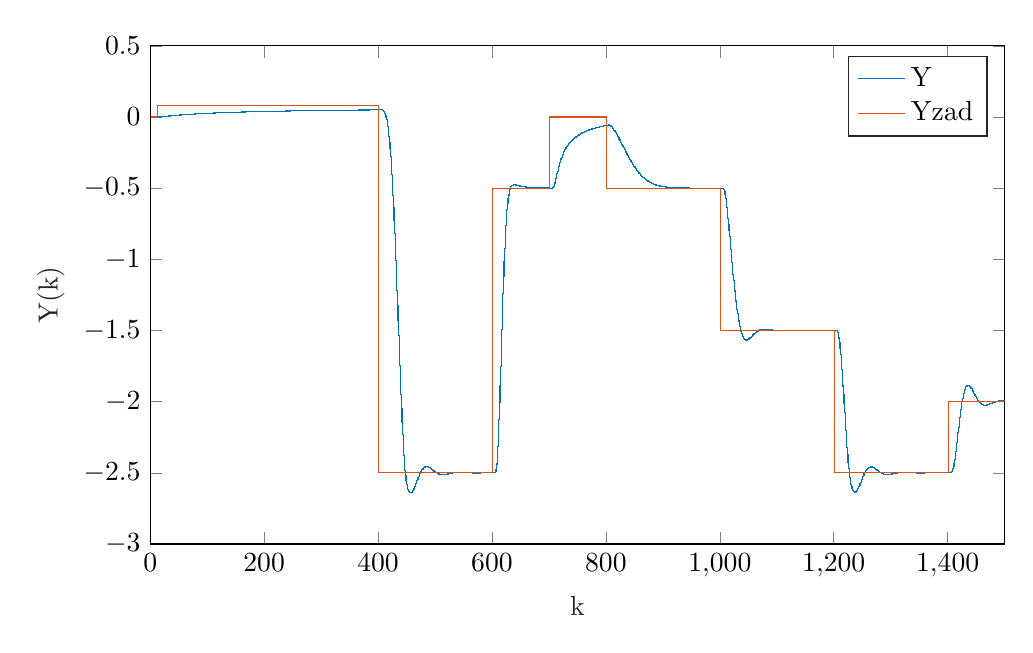
\begin{tikzpicture}

\begin{axis}[%
width=4.272in,
height=2.491in,
at={(0.717in,0.423in)},
scale only axis,
xmin=0,
xmax=1500,
xlabel style={font=\color{white!15!black}},
xlabel={k},
ymin=-3,
ymax=0.5,
ylabel style={font=\color{white!15!black}},
ylabel={Y(k)},
axis background/.style={fill=white},
legend style={legend cell align=left, align=left, draw=white!15!black}
]
\addplot[const plot, color=mycolor1] table[row sep=crcr] {%
1	0\\
2	0\\
3	0\\
4	0\\
5	0\\
6	0\\
7	0\\
8	0\\
9	0\\
10	0\\
11	0\\
12	0\\
13	0\\
14	0\\
15	0\\
16	0\\
17	6.50179751409729e-05\\
18	0.000254120359296923\\
19	0.000559358374099968\\
20	0.000949257041427869\\
21	0.00139087113863226\\
22	0.00185846939661365\\
23	0.00233505613463201\\
24	0.00281084178339463\\
25	0.00328097149875545\\
26	0.00374353398253461\\
27	0.00419814882581996\\
28	0.00464509869885649\\
29	0.00508486297986628\\
30	0.00551790532108378\\
31	0.00594460187034122\\
32	0.00636523630546835\\
33	0.00678001955168035\\
34	0.00718911344786295\\
35	0.00759265013462823\\
36	0.00799074528366106\\
37	0.00838350600186847\\
38	0.0087710349909606\\
39	0.00915343242050943\\
40	0.00953079657563858\\
41	0.00990322394433482\\
42	0.0102708091099263\\
43	0.0106336446214574\\
44	0.0109918209059385\\
45	0.0113454262333796\\
46	0.0116945467246633\\
47	0.0120392663876654\\
48	0.012379667169083\\
49	0.0127158290132659\\
50	0.0130478299228379\\
51	0.0133757460183983\\
52	0.0136996515961397\\
53	0.0140196191830502\\
54	0.014335719589751\\
55	0.0146480219611518\\
56	0.0149565938251271\\
57	0.0152615011393814\\
58	0.0155628083366392\\
59	0.0158605783682621\\
60	0.0161548727463732\\
61	0.0164457515845559\\
62	0.0167332736371856\\
63	0.0170174963374468\\
64	0.0172984758340872\\
65	0.0175762670269541\\
66	0.0178509236013629\\
67	0.018122498061338\\
68	0.0183910417617717\\
69	0.01865660493954\\
70	0.0189192367436156\\
71	0.0191789852642145\\
72	0.0194358975610135\\
73	0.0196900196904714\\
74	0.0199413967322882\\
75	0.0201900728150331\\
76	0.0204360911409714\\
77	0.0206794940101209\\
78	0.0209203228435627\\
79	0.0211586182060358\\
80	0.0213944198278401\\
81	0.0216277666260718\\
82	0.021858696725215\\
83	0.0220872474771134\\
84	0.0223134554803416\\
85	0.0225373565989985\\
86	0.0227589859809423\\
87	0.0229783780754865\\
88	0.0231955666505743\\
89	0.0234105848094516\\
90	0.0236234650068528\\
91	0.0238342390647177\\
92	0.0240429381874549\\
93	0.0242495929767663\\
94	0.0244542334460481\\
95	0.0246568890343817\\
96	0.0248575886201285\\
97	0.0250563605341413\\
98	0.0252532325726049\\
99	0.025448232009518\\
100	0.025641385608828\\
101	0.0258327196362304\\
102	0.0260222598706419\\
103	0.0262100316153602\\
104	0.0263960597089177\\
105	0.0265803685356415\\
106	0.0267629820359261\\
107	0.0269439237162311\\
108	0.0271232166588086\\
109	0.0273008835311729\\
110	0.0274769465953168\\
111	0.0276514277166846\\
112	0.0278243483729089\\
113	0.0279957296623169\\
114	0.028165592312216\\
115	0.0283339566869623\\
116	0.0285008427958212\\
117	0.0286662703006241\\
118	0.0288302585232295\\
119	0.0289928264527925\\
120	0.0291539927528491\\
121	0.0293137757682209\\
122	0.0294721935317458\\
123	0.0296292637708384\\
124	0.0297850039138869\\
125	0.0299394310964899\\
126	0.030092562167538\\
127	0.0302444136951456\\
128	0.0303950019724357\\
129	0.0305443430231834\\
130	0.0306924526073204\\
131	0.0308393462263066\\
132	0.0309850391283703\\
133	0.0311295463136228\\
134	0.031272882539049\\
135	0.0314150623233791\\
136	0.0315560999518433\\
137	0.0316960094808139\\
138	0.0318348047423375\\
139	0.0319724993485595\\
140	0.0321091066960454\\
141	0.0322446399700006\\
142	0.0323791121483916\\
143	0.0325125360059715\\
144	0.0326449241182124\\
145	0.0327762888651474\\
146	0.0329066424351233\\
147	0.0330359968284685\\
148	0.0331643638610767\\
149	0.0332917551679093\\
150	0.0334181822064186\\
151	0.0335436562598934\\
152	0.0336681884407302\\
153	0.0337917896936302\\
154	0.0339144707987258\\
155	0.0340362423746373\\
156	0.0341571148814617\\
157	0.0342770986236961\\
158	0.0343962037530964\\
159	0.0345144402714731\\
160	0.0346318180334272\\
161	0.0347483467490254\\
162	0.034864035986418\\
163	0.0349788951743998\\
164	0.0350929336049167\\
165	0.0352061604355174\\
166	0.035318584691754\\
167	0.0354302152695302\\
168	0.0355410609374008\\
169	0.035651130338822\\
170	0.035760431994354\\
171	0.0358689743038184\\
172	0.035976765548409\\
173	0.03608381389276\\
174	0.0361901273869705\\
175	0.0362957139685866\\
176	0.0364005814645438\\
177	0.0365047375930684\\
178	0.0366081899655404\\
179	0.0367109460883183\\
180	0.0368130133645263\\
181	0.036914399095806\\
182	0.037015110484032\\
183	0.0371151546329933\\
184	0.0372145385500407\\
185	0.0373132691477008\\
186	0.0374113532452593\\
187	0.0375087975703104\\
188	0.0376056087602779\\
189	0.0377017933639045\\
190	0.0377973578427124\\
191	0.0378923085724355\\
192	0.0379866518444228\\
193	0.0380803938670153\\
194	0.038173540766895\\
195	0.0382660985904092\\
196	0.0383580733048676\\
197	0.0384494707998159\\
198	0.0385402968882835\\
199	0.0386305573080086\\
200	0.0387202577226391\\
201	0.038809403722911\\
202	0.0388980008278041\\
203	0.0389860544856764\\
204	0.0390735700753764\\
205	0.0391605529073353\\
206	0.0392470082246382\\
207	0.0393329412040752\\
208	0.0394183569571733\\
209	0.039503260531209\\
210	0.0395876569102022\\
211	0.0396715510158913\\
212	0.0397549477086914\\
213	0.0398378517886338\\
214	0.039920267996289\\
215	0.0400022010136725\\
216	0.0400836554651347\\
217	0.0401646359182338\\
218	0.0402451468845937\\
219	0.0403251928207462\\
220	0.0404047781289577\\
221	0.0404839071580418\\
222	0.040562584204157\\
223	0.0406408135115899\\
224	0.0407185992735249\\
225	0.0407959456328004\\
226	0.0408728566826513\\
227	0.0409493364674386\\
228	0.041025388983366\\
229	0.0411010181791844\\
230	0.0411762279568835\\
231	0.0412510221723722\\
232	0.0413254046361463\\
233	0.0413993791139449\\
234	0.0414729493273963\\
235	0.0415461189546515\\
236	0.0416188916310077\\
237	0.0416912709495208\\
238	0.0417632604616078\\
239	0.0418348636776384\\
240	0.0419060840675169\\
241	0.0419769250612545\\
242	0.0420473900495313\\
243	0.0421174823842495\\
244	0.0421872053790771\\
245	0.042256562309982\\
246	0.0423255564157583\\
247	0.0423941908985426\\
248	0.0424624689243226\\
249	0.042530393623437\\
250	0.0425979680910673\\
251	0.0426651953877209\\
252	0.0427320785397073\\
253	0.0427986205396057\\
254	0.042864824346725\\
255	0.0429306928875571\\
256	0.0429962290562216\\
257	0.0430614357149044\\
258	0.0431263156942889\\
259	0.0431908717939797\\
260	0.0432551067829202\\
261	0.0433190233998034\\
262	0.0433826243534757\\
263	0.0434459123233348\\
264	0.0435088899597207\\
265	0.0435715598843013\\
266	0.0436339246904511\\
267	0.0436959869436242\\
268	0.0437577491817219\\
269	0.0438192139154538\\
270	0.0438803836286936\\
271	0.0439412607788296\\
272	0.044001847797109\\
273	0.0440621470889778\\
274	0.0441221610344149\\
275	0.0441818919882606\\
276	0.0442413422805413\\
277	0.0443005142167881\\
278	0.0443594100783504\\
279	0.0444180321227062\\
280	0.0444763825837657\\
281	0.0445344636721718\\
282	0.0445922775755951\\
283	0.0446498264590251\\
284	0.0447071124650566\\
285	0.0447641377141718\\
286	0.0448209043050181\\
287	0.0448774143146825\\
288	0.0449336697989606\\
289	0.0449896727926227\\
290	0.0450454253096751\\
291	0.0451009293436186\\
292	0.0451561868677019\\
293	0.045211199835172\\
294	0.045265970179521\\
295	0.045320499814729\\
296	0.0453747906355032\\
297	0.0454288445175142\\
298	0.0454826633176281\\
299	0.0455362488741358\\
300	0.0455896030069788\\
301	0.0456427275179713\\
302	0.04569562419102\\
303	0.0457482947923395\\
304	0.045800741070666\\
305	0.045852964757467\\
306	0.0459049675671479\\
307	0.0459567511972564\\
308	0.0460083173286835\\
309	0.0460596676258613\\
310	0.0461108037369591\\
311	0.0461617272940755\\
312	0.0462124399134285\\
313	0.0462629431955428\\
314	0.0463132387254343\\
315	0.0463633280727922\\
316	0.0464132127921585\\
317	0.0464628944231051\\
318	0.046512374490408\\
319	0.0465616545042197\\
320	0.0466107359602388\\
321	0.0466596203398773\\
322	0.0467083091104258\\
323	0.0467568037252164\\
324	0.0468051056237827\\
325	0.0468532162320189\\
326	0.0469011369623356\\
327	0.0469488692138137\\
328	0.0469964143723569\\
329	0.047043773810841\\
330	0.0470909488892623\\
331	0.0471379409548831\\
332	0.047184751342376\\
333	0.0472313813739653\\
334	0.0472778323595679\\
335	0.0473241055969306\\
336	0.0473702023717672\\
337	0.0474161239578926\\
338	0.0474618716173556\\
339	0.0475074466005701\\
340	0.0475528501464442\\
341	0.0475980834825077\\
342	0.0476431478250382\\
343	0.0476880443791848\\
344	0.0477327743390914\\
345	0.047777338888017\\
346	0.0478217391984555\\
347	0.0478659764322534\\
348	0.0479100517407261\\
349	0.0479539662647728\\
350	0.0479977211349896\\
351	0.0480413174717815\\
352	0.0480847563854727\\
353	0.0481280389764158\\
354	0.0481711663350991\\
355	0.0482141395422528\\
356	0.0482569596689541\\
357	0.0482996277767306\\
358	0.0483421449176623\\
359	0.0483845121344827\\
360	0.0484267304606784\\
361	0.0484688009205872\\
362	0.0485107245294956\\
363	0.0485525022937343\\
364	0.0485941352107732\\
365	0.0486356242693145\\
366	0.0486769704493855\\
367	0.0487181747224295\\
368	0.0487592380513956\\
369	0.0488001613908282\\
370	0.0488409456869542\\
371	0.0488815918777701\\
372	0.0489221008931273\\
373	0.0489624736548173\\
374	0.0490027110766545\\
375	0.0490428140645592\\
376	0.049082783516639\\
377	0.0491226203232692\\
378	0.0491623253671725\\
379	0.0492018995234973\\
380	0.0492413436598956\\
381	0.0492806586365996\\
382	0.0493198453064971\\
383	0.0493589045152067\\
384	0.0493978371011515\\
385	0.0494366438956324\\
386	0.0494753257228999\\
387	0.0495138834002255\\
388	0.049552317737972\\
389	0.0495906295396635\\
390	0.0496288196020538\\
391	0.0496668887151942\\
392	0.0497048376625012\\
393	0.0497426672208221\\
394	0.0497803781605012\\
395	0.0498179712454442\\
396	0.0498554472331824\\
397	0.0498928068749356\\
398	0.0499300509156752\\
399	0.0499671800941856\\
400	0.0500041951431252\\
401	0.0500410967890869\\
402	0.050077885752658\\
403	0.0501145627484786\\
404	0.0501511284853002\\
405	0.0501875836660434\\
406	0.0501836339158467\\
407	0.0490143636731005\\
408	0.0465386297714727\\
409	0.0427663380041105\\
410	0.0376166249535764\\
411	0.0308727678545499\\
412	0.022194648415639\\
413	0.0111458250845424\\
414	-0.0027774645058538\\
415	-0.0201175092650681\\
416	-0.0414263887353383\\
417	-0.0672375924534622\\
418	-0.0980391711668627\\
419	-0.134250097302705\\
420	-0.17620145905712\\
421	-0.224123608229261\\
422	-0.278139635218797\\
423	-0.338264787032206\\
424	-0.40441083325637\\
425	-0.476394026460228\\
426	-0.553945215924974\\
427	-0.636720810879519\\
428	-0.724313574723378\\
429	-0.81626258089203\\
430	-0.912062002164359\\
431	-1.01116868899618\\
432	-1.11300869405603\\
433	-1.21698301546391\\
434	-1.32247287055642\\
435	-1.42884479325323\\
436	-1.53545579139702\\
437	-1.64165872436546\\
438	-1.74680798083716\\
439	-1.85026546260582\\
440	-1.95140681945188\\
441	-2.04962783549518\\
442	-2.14353019428333\\
443	-2.23040191194809\\
444	-2.30823246023429\\
445	-2.37617028748871\\
446	-2.43416500227336\\
447	-2.48269248319694\\
448	-2.5225482617383\\
449	-2.55469610601636\\
450	-2.58016043596014\\
451	-2.59995289501101\\
452	-2.61502500633454\\
453	-2.62616386945973\\
454	-2.63395826231364\\
455	-2.63884984106348\\
456	-2.64118638933321\\
457	-2.64125751836288\\
458	-2.63931759982415\\
459	-2.63559993771718\\
460	-2.63032512607673\\
461	-2.62370559797571\\
462	-2.61594770728831\\
463	-2.60725224164518\\
464	-2.59781397128572\\
465	-2.58782064345634\\
466	-2.57745170147581\\
467	-2.56687691916483\\
468	-2.55625508045119\\
469	-2.54573279119219\\
470	-2.53544347952882\\
471	-2.52550661850097\\
472	-2.51602718771755\\
473	-2.50709537800349\\
474	-2.49878653312629\\
475	-2.49116131528585\\
476	-2.48426607559399\\
477	-2.4781334069644\\
478	-2.47278285443274\\
479	-2.46822175672261\\
480	-2.46444619267311\\
481	-2.46144200676642\\
482	-2.4591858892647\\
483	-2.45764648822282\\
484	-2.45678553273553\\
485	-2.45655894907307\\
486	-2.45691795374225\\
487	-2.45781010988702\\
488	-2.4591803357406\\
489	-2.46097185600526\\
490	-2.46312708903005\\
491	-2.46558846446113\\
492	-2.4682991676445\\
493	-2.47120380847059\\
494	-2.4742490135724\\
495	-2.47738394183963\\
496	-2.48056072410636\\
497	-2.4837348286293\\
498	-2.48686535461388\\
499	-2.48991525658583\\
500	-2.49285150285872\\
501	-2.49564517172888\\
502	-2.4982714893464\\
503	-2.5007098134742\\
504	-2.50294356756119\\
505	-2.50496012972555\\
506	-2.50675068137121\\
507	-2.50831002024709\\
508	-2.50963634280393\\
509	-2.51073100070812\\
510	-2.51159823633487\\
511	-2.51224490198438\\
512	-2.51268016744441\\
513	-2.51291522036095\\
514	-2.51296296367774\\
515	-2.51283771416595\\
516	-2.51255490579163\\
517	-2.51213080136268\\
518	-2.51158221556505\\
519	-2.5109262521429\\
520	-2.51018005760677\\
521	-2.50936059347137\\
522	-2.50848442863832\\
523	-2.50756755315343\\
524	-2.50662521418999\\
525	-2.50567177474341\\
526	-2.50472059517518\\
527	-2.50378393741784\\
528	-2.50287289135367\\
529	-2.50199732260904\\
530	-2.50116584076811\\
531	-2.50038578680383\\
532	-2.49966323835294\\
533	-2.49900303132426\\
534	-2.49840879622565\\
535	-2.49788300752378\\
536	-2.49742704430988\\
537	-2.49704126053264\\
538	-2.4967250630734\\
539	-2.49647699597642\\
540	-2.49629482920517\\
541	-2.49617565037212\\
542	-2.49611595798037\\
543	-2.49611175481925\\
544	-2.49615864026853\\
545	-2.49625190038631\\
546	-2.49638659477948\\
547	-2.49655763938317\\
548	-2.49675988440218\\
549	-2.49698818679394\\
550	-2.49723747679514\\
551	-2.4975028181133\\
552	-2.49777946151771\\
553	-2.49806289167165\\
554	-2.4983488671477\\
555	-2.49863345366015\\
556	-2.4989130506332\\
557	-2.49918441129887\\
558	-2.49944465658606\\
559	-2.49969128312018\\
560	-2.49992216570263\\
561	-2.50013555468025\\
562	-2.50033006864756\\
563	-2.50050468294879\\
564	-2.50065871446383\\
565	-2.50079180317091\\
566	-2.50090389098153\\
567	-2.50099519833905\\
568	-2.5010661990619\\
569	-2.50111759389775\\
570	-2.50115028323406\\
571	-2.50116533938689\\
572	-2.50116397886167\\
573	-2.50114753494908\\
574	-2.50111743098637\\
575	-2.50107515457939\\
576	-2.50102223304513\\
577	-2.50096021029804\\
578	-2.50089062536674\\
579	-2.50081499269194\\
580	-2.50073478432087\\
581	-2.50065141407985\\
582	-2.50056622377384\\
583	-2.50048047143178\\
584	-2.50039532158794\\
585	-2.50031183756361\\
586	-2.50023097569008\\
587	-2.5001535813931\\
588	-2.50008038704102\\
589	-2.50001201144321\\
590	-2.49994896087324\\
591	-2.49989163148087\\
592	-2.49984031294995\\
593	-2.49979519325425\\
594	-2.49975636436088\\
595	-2.4997238287305\\
596	-2.49969750646528\\
597	-2.49967724295909\\
598	-2.49966281690955\\
599	-2.49965394855805\\
600	-2.4996503080318\\
601	-2.49965152367061\\
602	-2.49965719023099\\
603	-2.49966687687007\\
604	-2.49968013482302\\
605	-2.49969650469814\\
606	-2.49315417534655\\
607	-2.47379559731194\\
608	-2.43809365724904\\
609	-2.38458440610647\\
610	-2.31332480243043\\
611	-2.22547722150465\\
612	-2.12300345579478\\
613	-2.00843423266691\\
614	-1.88468358516637\\
615	-1.75488684978831\\
616	-1.62224995127145\\
617	-1.48990497436371\\
618	-1.36077300528126\\
619	-1.23743985455511\\
620	-1.12205314944217\\
621	-1.01624985707308\\
622	-0.921121304008205\\
623	-0.837218552004997\\
624	-0.764595656130275\\
625	-0.702883288467733\\
626	-0.651381758134208\\
627	-0.609161306303552\\
628	-0.575158657861434\\
629	-0.548261521460125\\
630	-0.527376134586391\\
631	-0.511476210906287\\
632	-0.499634208091861\\
633	-0.491037473144574\\
634	-0.484992583044273\\
635	-0.480921278314778\\
636	-0.478351029833717\\
637	-0.476902705240087\\
638	-0.476277174218059\\
639	-0.476242113630691\\
640	-0.476619794331738\\
641	-0.477276265844743\\
642	-0.478112095863382\\
643	-0.479054651308511\\
644	-0.480051806142247\\
645	-0.481066909157969\\
646	-0.482074826511329\\
647	-0.483058876418196\\
648	-0.484008488183533\\
649	-0.484917438318701\\
650	-0.485782538911013\\
651	-0.48660267517966\\
652	-0.487378108946341\\
653	-0.488109981962123\\
654	-0.488799967520595\\
655	-0.48945003067693\\
656	-0.49006226694931\\
657	-0.490638796926838\\
658	-0.491181700077577\\
659	-0.491692975551053\\
660	-0.492174521175665\\
661	-0.492628124396809\\
662	-0.493055460780044\\
663	-0.493458097072481\\
664	-0.493837496799891\\
665	-0.494195027074776\\
666	-0.494531965777471\\
667	-0.494849508605815\\
668	-0.495148775712485\\
669	-0.495430817794871\\
670	-0.49569662159411\\
671	-0.495947114814671\\
672	-0.496183170506053\\
673	-0.496405610962297\\
674	-0.496615211199164\\
675	-0.496812702067079\\
676	-0.496998773052971\\
677	-0.49717407481777\\
678	-0.497339221509526\\
679	-0.497494792885687\\
680	-0.497641336272196\\
681	-0.497779368381974\\
682	-0.497909377011078\\
683	-0.498031822627262\\
684	-0.498147139862785\\
685	-0.498255738921025\\
686	-0.498358006904644\\
687	-0.498454309071644\\
688	-0.498544990024551\\
689	-0.498630374837151\\
690	-0.498710770122551\\
691	-0.498786465045874\\
692	-0.498857732284514\\
693	-0.498924828938606\\
694	-0.498987997394158\\
695	-0.499047466141119\\
696	-0.499103450548513\\
697	-0.499156153598681\\
698	-0.499205766582558\\
699	-0.499252469757847\\
700	-0.499296432971856\\
701	-0.499337816250723\\
702	-0.499376770356667\\
703	-0.499413437314837\\
704	-0.499447950911289\\
705	-0.499480437163546\\
706	-0.498026267585271\\
707	-0.493908369913518\\
708	-0.486738878704985\\
709	-0.476641704642449\\
710	-0.464035096340439\\
711	-0.449475030108534\\
712	-0.433551001148837\\
713	-0.416821260081072\\
714	-0.399776006043803\\
715	-0.382819897466085\\
716	-0.366267627690076\\
717	-0.350348021611676\\
718	-0.335213307911286\\
719	-0.3209510924825\\
720	-0.30759722851036\\
721	-0.295148318125716\\
722	-0.283573023590023\\
723	-0.272821723411294\\
724	-0.262834329767774\\
725	-0.253546289316543\\
726	-0.244892926797076\\
727	-0.236812369929243\\
728	-0.229247326610191\\
729	-0.222145983682918\\
730	-0.215462272241797\\
731	-0.209155707552905\\
732	-0.2031909700211\\
733	-0.197537352784949\\
734	-0.192168164952714\\
735	-0.187060149001224\\
736	-0.182192946975075\\
737	-0.17754863252784\\
738	-0.173111313727232\\
739	-0.168866803868435\\
740	-0.164802353241711\\
741	-0.160906432911209\\
742	-0.157168561266231\\
743	-0.153579164764874\\
744	-0.150129465434555\\
745	-0.14681138900427\\
746	-0.14361748881955\\
747	-0.14054088182269\\
748	-0.137575193821121\\
749	-0.134714512009495\\
750	-0.131953343273422\\
751	-0.1292865772135\\
752	-0.126709453118706\\
753	-0.124217530318196\\
754	-0.121806661475492\\
755	-0.119472968479127\\
756	-0.117212820644322\\
757	-0.115022814981978\\
758	-0.112899758321568\\
759	-0.110840651097975\\
760	-0.108842672631876\\
761	-0.106903167750409\\
762	-0.105019634610384\\
763	-0.103189713600566\\
764	-0.101411177212696\\
765	-0.0996819207828884\\
766	-0.0979999540159383\\
767	-0.0963633932148472\\
768	-0.0947704541465637\\
769	-0.0932194454826663\\
770	-0.091708762760494\\
771	-0.0902368828162081\\
772	-0.0888023586464978\\
773	-0.087403814660244\\
774	-0.0860399422854885\\
775	-0.0847094959006112\\
776	-0.0834112890617509\\
777	-0.0821441910012775\\
778	-0.0809071233745831\\
779	-0.0796990572346405\\
780	-0.0785190102157277\\
781	-0.0773660439094526\\
782	-0.0762392614177674\\
783	-0.0751378050690544\\
784	-0.0740608542846176\\
785	-0.0730076235840354\\
786	-0.0719773607188451\\
787	-0.0709693449249385\\
788	-0.0699828852848757\\
789	-0.0690173191920629\\
790	-0.0680720109094197\\
791	-0.0671463502157654\\
792	-0.0662397511337123\\
793	-0.0653516507333518\\
794	-0.0644815080064806\\
795	-0.0636288028065261\\
796	-0.0627930348497111\\
797	-0.0619737227733429\\
798	-0.0611704032474261\\
799	-0.0603826301360899\\
800	-0.0596099737055794\\
801	-0.0588520198758066\\
802	-0.0581083695126754\\
803	-0.0573786377585983\\
804	-0.0566624533988095\\
805	-0.0559594582612498\\
806	-0.05599482184391\\
807	-0.057329414284851\\
808	-0.0599954452438591\\
809	-0.0637939263653131\\
810	-0.0684647936394835\\
811	-0.0737700537611499\\
812	-0.0795238444364701\\
813	-0.0855947622565116\\
814	-0.0918965884392081\\
815	-0.0983761346530858\\
816	-0.105002203771317\\
817	-0.111757028586719\\
818	-0.118630266214455\\
819	-0.125615110755799\\
820	-0.132705966552805\\
821	-0.139897179169768\\
822	-0.147182433451244\\
823	-0.154554543613936\\
824	-0.162005454378352\\
825	-0.169526341796754\\
826	-0.177107750290565\\
827	-0.184739732906071\\
828	-0.192411979992082\\
829	-0.200113931560907\\
830	-0.207834873596635\\
831	-0.215564020637048\\
832	-0.223290587440737\\
833	-0.231003852286466\\
834	-0.238693213907384\\
835	-0.246348243483056\\
836	-0.253958732608647\\
837	-0.261514737769707\\
838	-0.269006621572564\\
839	-0.2764250907976\\
840	-0.283761231234498\\
841	-0.291006539204864\\
842	-0.298152949661498\\
843	-0.305192860762219\\
844	-0.312119154839754\\
845	-0.318925215721372\\
846	-0.325604942387853\\
847	-0.332152758998286\\
848	-0.338563621342967\\
849	-0.344833019820294\\
850	-0.350956979064207\\
851	-0.356932054376085\\
852	-0.362755325138825\\
853	-0.368424385411037\\
854	-0.373937331915911\\
855	-0.379292749652383\\
856	-0.384489695365835\\
857	-0.389527679121924\\
858	-0.394406644230277\\
859	-0.399126945765063\\
860	-0.403689327926892\\
861	-0.408094900485473\\
862	-0.412345114535163\\
863	-0.416441737786181\\
864	-0.420386829603184\\
865	-0.424182715990318\\
866	-0.427831964708054\\
867	-0.431337360692356\\
868	-0.434701881931259\\
869	-0.437928675938055\\
870	-0.441021036944099\\
871	-0.443982383918195\\
872	-0.446816239503521\\
873	-0.449526209947575\\
874	-0.452115966085596\\
875	-0.454589225423595\\
876	-0.456949735353632\\
877	-0.459201257521327\\
878	-0.461347553353949\\
879	-0.463392370746738\\
880	-0.465339431895563\\
881	-0.467192422255406\\
882	-0.468954980596732\\
883	-0.470630690125304\\
884	-0.472223070625588\\
885	-0.473735571583393\\
886	-0.475171566239839\\
887	-0.476534346526042\\
888	-0.47782711882598\\
889	-0.479053000513832\\
890	-0.480215017211553\\
891	-0.481316100712512\\
892	-0.482359087517587\\
893	-0.483346717931152\\
894	-0.484281635665806\\
895	-0.485166387906407\\
896	-0.486003425785993\\
897	-0.486795105228349\\
898	-0.487543688114351\\
899	-0.488251343731677\\
900	-0.488920150469998\\
901	-0.489552097726353\\
902	-0.490149087987946\\
903	-0.490712939062156\\
904	-0.491245386426036\\
905	-0.491748085669985\\
906	-0.492222615012604\\
907	-0.492670477865978\\
908	-0.493093105432739\\
909	-0.493491859318271\\
910	-0.493868034143304\\
911	-0.494222860143882\\
912	-0.494557505747371\\
913	-0.494873080114632\\
914	-0.495170635639922\\
915	-0.495451170401348\\
916	-0.495715630555864\\
917	-0.495964912673861\\
918	-0.496199866009372\\
919	-0.49642129470274\\
920	-0.496629959913413\\
921	-0.496826581881178\\
922	-0.497011841914771\\
923	-0.497186384307333\\
924	-0.497350818178647\\
925	-0.497505719244501\\
926	-0.497651631513857\\
927	-0.49778906891484\\
928	-0.49791851685077\\
929	-0.498040433687704\\
930	-0.498155252175119\\
931	-0.498263380801506\\
932	-0.498365205086752\\
933	-0.498461088813288\\
934	-0.498551375198024\\
935	-0.498636388007144\\
936	-0.498716432615856\\
937	-0.498791797015194\\
938	-0.498862752767975\\
939	-0.498929555915986\\
940	-0.498992447840457\\
941	-0.499051656077839\\
942	-0.499107395092859\\
943	-0.499159867010797\\
944	-0.499209262310846\\
945	-0.499255760482399\\
946	-0.499299530646024\\
947	-0.499340732140826\\
948	-0.499379515079864\\
949	-0.4994160208752\\
950	-0.499450382734103\\
951	-0.499482726127882\\
952	-0.49951316923475\\
953	-0.499541823358059\\
954	-0.499568793321201\\
955	-0.499594177840394\\
956	-0.499618069876533\\
957	-0.499640556967221\\
958	-0.499661721540043\\
959	-0.499681641208102\\
960	-0.499700389048774\\
961	-0.499718033866607\\
962	-0.499734640441223\\
963	-0.499750269761064\\
964	-0.499764979243754\\
965	-0.499778822943825\\
966	-0.499791851748513\\
967	-0.49980411356229\\
968	-0.499815653480764\\
969	-0.499826513954554\\
970	-0.499836734943683\\
971	-0.499846354063063\\
972	-0.499855406719538\\
973	-0.499863926240994\\
974	-0.499871943997976\\
975	-0.499879489518242\\
976	-0.499886590594657\\
977	-0.499893273386811\\
978	-0.499899562516725\\
979	-0.499905481158972\\
980	-0.499911051125554\\
981	-0.499916292945818\\
982	-0.499921225941713\\
983	-0.49992586829865\\
984	-0.499930237132218\\
985	-0.499934348550999\\
986	-0.499938217715716\\
987	-0.499941858894908\\
988	-0.499945285517353\\
989	-0.499948510221417\\
990	-0.499951544901513\\
991	-0.499954400751836\\
992	-0.499957088307532\\
993	-0.499959617483455\\
994	-0.49996199761065\\
995	-0.499964237470691\\
996	-0.499966345328007\\
997	-0.499968328960309\\
998	-0.49997019568723\\
999	-0.49997195239728\\
1000	-0.499973605573223\\
1001	-0.499975161315958\\
1002	-0.499976625366995\\
1003	-0.499978003129616\\
1004	-0.499979299688785\\
1005	-0.499980519829893\\
1006	-0.50289059035812\\
1007	-0.511000564263743\\
1008	-0.525142230273076\\
1009	-0.545271074542855\\
1010	-0.57087273704416\\
1011	-0.601223562867451\\
1012	-0.635542779136751\\
1013	-0.673073265966794\\
1014	-0.713118969493863\\
1015	-0.755057656754102\\
1016	-0.798340685956847\\
1017	-0.842486735781139\\
1018	-0.887073420288094\\
1019	-0.931728864123174\\
1020	-0.976124216788084\\
1021	-1.01996746372297\\
1022	-1.06299855939504\\
1023	-1.10498574990921\\
1024	-1.14572288753065\\
1025	-1.18502752769572\\
1026	-1.22273961390556\\
1027	-1.25872058132403\\
1028	-1.29285273797954\\
1029	-1.32503880926008\\
1030	-1.35520155523382\\
1031	-1.38328339078262\\
1032	-1.40924595575847\\
1033	-1.43306959676816\\
1034	-1.45475273422663\\
1035	-1.47431109843001\\
1036	-1.49177682694977\\
1037	-1.50719742292317\\
1038	-1.52063458001674\\
1039	-1.53216288510724\\
1040	-1.54186841414119\\
1041	-1.5498472402447\\
1042	-1.55620387597545\\
1043	-1.561049673641\\
1044	-1.5645012088502\\
1045	-1.56667867291917\\
1046	-1.56770429943661\\
1047	-1.56770084923738\\
1048	-1.566790176292\\
1049	-1.56509189466929\\
1050	-1.56272216386607\\
1051	-1.55979260653572\\
1052	-1.55640936911457\\
1053	-1.55267233217458\\
1054	-1.5486744736593\\
1055	-1.54450138461394\\
1056	-1.54023093371837\\
1057	-1.53593307397019\\
1058	-1.5316697823222\\
1059	-1.52749512100681\\
1060	-1.52345540770771\\
1061	-1.51958948067063\\
1062	-1.51592904426365\\
1063	-1.51249908036687\\
1064	-1.50931831124261\\
1065	-1.50639970014997\\
1066	-1.50375097685674\\
1067	-1.50137517630024\\
1068	-1.49927117989124\\
1069	-1.49743425028173\\
1070	-1.49585655177351\\
1071	-1.49452764988569\\
1072	-1.49343498488712\\
1073	-1.49256431530682\\
1074	-1.49190012854143\\
1075	-1.4914260166706\\
1076	-1.49112501646343\\
1077	-1.49097991331005\\
1078	-1.490973509446\\
1079	-1.49108885735947\\
1080	-1.49130945969154\\
1081	-1.49161943726662\\
1082	-1.4920036671359\\
1083	-1.49244789268989\\
1084	-1.49293880800868\\
1085	-1.4934641186789\\
1086	-1.49401258132342\\
1087	-1.49457402407199\\
1088	-1.49513935015373\\
1089	-1.49570052672311\\
1090	-1.49625056094364\\
1091	-1.49678346525252\\
1092	-1.49729421361864\\
1093	-1.49777869048861\\
1094	-1.49823363399251\\
1095	-1.49865657485625\\
1096	-1.49904577234112\\
1097	-1.49940014840554\\
1098	-1.49971922115996\\
1099	-1.50000303856464\\
1100	-1.50025211320212\\
1101	-1.50046735884284\\
1102	-1.5006500294134\\
1103	-1.5008016608742\\
1104	-1.50092401641548\\
1105	-1.50101903529014\\
1106	-1.50108878551702\\
1107	-1.50113542061101\\
1108	-1.50116114042554\\
1109	-1.50116815612943\\
1110	-1.50115865928369\\
1111	-1.50113479493393\\
1112	-1.50109863859166\\
1113	-1.50105217694115\\
1114	-1.50099729207896\\
1115	-1.50093574906922\\
1116	-1.50086918657968\\
1117	-1.50079911035051\\
1118	-1.50072688923977\\
1119	-1.50065375358587\\
1120	-1.50058079562732\\
1121	-1.50050897172408\\
1122	-1.5004391061312\\
1123	-1.50037189608511\\
1124	-1.50030791797398\\
1125	-1.50024763437698\\
1126	-1.50019140177157\\
1127	-1.50013947872364\\
1128	-1.50009203439111\\
1129	-1.50004915718836\\
1130	-1.50001086347517\\
1131	-1.49997710615023\\
1132	-1.49994778304539\\
1133	-1.49992274503202\\
1134	-1.49990180376583\\
1135	-1.49988473901018\\
1136	-1.49987130549124\\
1137	-1.49986123925008\\
1138	-1.49985426346802\\
1139	-1.49985009375159\\
1140	-1.49984844287226\\
1141	-1.49984902496412\\
1142	-1.49985155918961\\
1143	-1.49985577288922\\
1144	-1.4998614042361\\
1145	-1.49986820442066\\
1146	-1.49987593939336\\
1147	-1.49988439119643\\
1148	-1.49989335891699\\
1149	-1.49990265929518\\
1150	-1.49991212702124\\
1151	-1.49992161475582\\
1152	-1.49993099290692\\
1153	-1.49994014919633\\
1154	-1.49994898804711\\
1155	-1.49995742982221\\
1156	-1.49996540994261\\
1157	-1.49997287791153\\
1158	-1.49997979626929\\
1159	-1.49998613950127\\
1160	-1.4999918929194\\
1161	-1.49999705153526\\
1162	-1.50000161894105\\
1163	-1.50000560621243\\
1164	-1.50000903084511\\
1165	-1.5000119157356\\
1166	-1.500014288214\\
1167	-1.50001617913582\\
1168	-1.50001762203743\\
1169	-1.50001865235893\\
1170	-1.50001930673648\\
1171	-1.50001962236511\\
1172	-1.50001963643197\\
1173	-1.50001938561891\\
1174	-1.50001890567273\\
1175	-1.50001823104041\\
1176	-1.5000173945664\\
1177	-1.50001642724841\\
1178	-1.50001535804774\\
1179	-1.50001421375017\\
1180	-1.50001301887294\\
1181	-1.50001179561355\\
1182	-1.50001056383592\\
1183	-1.50000934108942\\
1184	-1.50000814265674\\
1185	-1.50000698162616\\
1186	-1.50000586898449\\
1187	-1.5000048137267\\
1188	-1.50000382297895\\
1189	-1.50000290213156\\
1190	-1.50000205497901\\
1191	-1.50000128386421\\
1192	-1.50000058982457\\
1193	-1.49999997273771\\
1194	-1.49999943146492\\
1195	-1.49999896399067\\
1196	-1.49999856755683\\
1197	-1.49999823879044\\
1198	-1.49999797382408\\
1199	-1.49999776840816\\
1200	-1.49999761801458\\
1201	-1.49999751793151\\
1202	-1.49999746334894\\
1203	-1.4999974494352\\
1204	-1.49999747140434\\
1205	-1.49999752457468\\
1206	-1.50318691673941\\
1207	-1.51234618191506\\
1208	-1.52882620624714\\
1209	-1.55301640224091\\
1210	-1.58469624363117\\
1211	-1.6232823130964\\
1212	-1.667991483502\\
1213	-1.71794475450123\\
1214	-1.77223167590928\\
1215	-1.82994932282807\\
1216	-1.89022513797257\\
1217	-1.95222974542645\\
1218	-2.01518369463373\\
1219	-2.07836067063304\\
1220	-2.14108876378145\\
1221	-2.20275076919406\\
1222	-2.26278407657762\\
1223	-2.32068045009496\\
1224	-2.37489201692976\\
1225	-2.42397975171795\\
1226	-2.46720624937081\\
1227	-2.50438942952643\\
1228	-2.5357195264173\\
1229	-2.56162040891507\\
1230	-2.58264697436869\\
1231	-2.59941137331647\\
1232	-2.61251392664626\\
1233	-2.62242952138928\\
1234	-2.62951672112526\\
1235	-2.63406065514428\\
1236	-2.63630246814625\\
1237	-2.63645840735913\\
1238	-2.63473152924997\\
1239	-2.63131844913447\\
1240	-2.62641282862746\\
1241	-2.62020674029918\\
1242	-2.61289067529313\\
1243	-2.60465271149733\\
1244	-2.5956771953415\\
1245	-2.58614318048096\\
1246	-2.57622279235107\\
1247	-2.56607963637287\\
1248	-2.55586733142352\\
1249	-2.54572822389748\\
1250	-2.53579231799205\\
1251	-2.5261764426807\\
1252	-2.51698366389853\\
1253	-2.50830294095983\\
1254	-2.50020901866983\\
1255	-2.4927625406748\\
1256	-2.48601036511279\\
1257	-2.47998606042651\\
1258	-2.47471055714459\\
1259	-2.47019293039646\\
1260	-2.46643128776246\\
1261	-2.46341373763414\\
1262	-2.46111941442775\\
1263	-2.45951953861685\\
1264	-2.458578491495\\
1265	-2.45825488672697\\
1266	-2.45850262299061\\
1267	-2.45927190426384\\
1268	-2.46051021650154\\
1269	-2.46216325152275\\
1270	-2.46417577085321\\
1271	-2.46649240401968\\
1272	-2.46905837736135\\
1273	-2.47182017080874\\
1274	-2.47472610129036\\
1275	-2.47772683247259\\
1276	-2.4807758114351\\
1277	-2.48382963364856\\
1278	-2.48684833827\\
1279	-2.48979563632041\\
1280	-2.49263907477203\\
1281	-2.49535013996253\\
1282	-2.49790430407979\\
1283	-2.50028101873148\\
1284	-2.5024636598352\\
1285	-2.50443942824068\\
1286	-2.50619921062851\\
1287	-2.50773740532192\\
1288	-2.5090517176988\\
1289	-2.51014292990169\\
1290	-2.51101464951292\\
1291	-2.51167304179086\\
1292	-2.51212654995124\\
1293	-2.51238560782547\\
1294	-2.51246234903764\\
1295	-2.51237031661431\\
1296	-2.51212417668028\\
1297	-2.51173943960194\\
1298	-2.51123219162192\\
1299	-2.5106188396892\\
1300	-2.5099158718333\\
1301	-2.50913963506428\\
1302	-2.50830613240857\\
1303	-2.50743084031986\\
1304	-2.50652854733902\\
1305	-2.50561321452402\\
1306	-2.50469785783401\\
1307	-2.50379445233553\\
1308	-2.50291385780798\\
1309	-2.50206576506107\\
1310	-2.5012586620439\\
1311	-2.50049981862291\\
1312	-2.49979528873609\\
1313	-2.49914992849426\\
1314	-2.49856742869491\\
1315	-2.49805036014069\\
1316	-2.49760023011052\\
1317	-2.49721754831484\\
1318	-2.49690190067578\\
1319	-2.49665202930503\\
1320	-2.49646591710481\\
1321	-2.49634087548703\\
1322	-2.49627363379118\\
1323	-2.49626042907818\\
1324	-2.49629709508442\\
1325	-2.49637914923404\\
1326	-2.49650187672601\\
1327	-2.49666041083436\\
1328	-2.49684980868166\\
1329	-2.49706512186735\\
1330	-2.49730146145124\\
1331	-2.49755405690743\\
1332	-2.49781830877384\\
1333	-2.49808983482706\\
1334	-2.49836450970907\\
1335	-2.49863849802348\\
1336	-2.49890828100042\\
1337	-2.49917067690448\\
1338	-2.49942285542547\\
1339	-2.49966234634982\\
1340	-2.49988704285956\\
1341	-2.50009519984661\\
1342	-2.50028542766325\\
1343	-2.50045668175404\\
1344	-2.50060824863229\\
1345	-2.50073972867393\\
1346	-2.50085101620524\\
1347	-2.50094227735785\\
1348	-2.50101392615593\\
1349	-2.50106659928628\\
1350	-2.50110112998376\\
1351	-2.5011185214417\\
1352	-2.50111992013068\\
1353	-2.50110658938031\\
1354	-2.50107988354691\\
1355	-2.50104122305711\\
1356	-2.50099207058313\\
1357	-2.50093390857027\\
1358	-2.50086821830239\\
1359	-2.50079646065611\\
1360	-2.50072005866057\\
1361	-2.50064038194663\\
1362	-2.50055873313801\\
1363	-2.50047633620721\\
1364	-2.50039432679161\\
1365	-2.50031374443953\\
1366	-2.50023552673346\\
1367	-2.50016050521691\\
1368	-2.50008940303386\\
1369	-2.50002283417433\\
1370	-2.49996130420722\\
1371	-2.49990521237149\\
1372	-2.49985485488927\\
1373	-2.49981042935951\\
1374	-2.49977204008791\\
1375	-2.49973970420806\\
1376	-2.49971335845044\\
1377	-2.49969286641835\\
1378	-2.49967802623519\\
1379	-2.49966857843315\\
1380	-2.49966421396078\\
1381	-2.49966458219536\\
1382	-2.49966929885491\\
1383	-2.49967795371458\\
1384	-2.49969011804248\\
1385	-2.49970535168022\\
1386	-2.49972320970443\\
1387	-2.49974324861594\\
1388	-2.49976503201372\\
1389	-2.49978813572097\\
1390	-2.49981215234053\\
1391	-2.49983669522581\\
1392	-2.4998614018626\\
1393	-2.49988593666464\\
1394	-2.49990999319384\\
1395	-2.49993329582202\\
1396	-2.49995560085756\\
1397	-2.49997669716498\\
1398	-2.49999640631016\\
1399	-2.50001458226725\\
1400	-2.50003111072626\\
1401	-2.50004590804234\\
1402	-2.50005891986922\\
1403	-2.50007011951984\\
1404	-2.50007950609753\\
1405	-2.50008710244047\\
1406	-2.49847832011049\\
1407	-2.49374674839975\\
1408	-2.48506987904711\\
1409	-2.4721198532568\\
1410	-2.45491363603676\\
1411	-2.43370125876698\\
1412	-2.4088864029543\\
1413	-2.38097038762676\\
1414	-2.35051191602316\\
1415	-2.31809730089401\\
1416	-2.28431779660596\\
1417	-2.24975196151563\\
1418	-2.21495179707918\\
1419	-2.18043191290777\\
1420	-2.14666126146589\\
1421	-2.11405714732973\\
1422	-2.08298129397009\\
1423	-2.0537377762352\\
1424	-2.02657262652614\\
1425	-2.00167490925469\\
1426	-1.97917904230844\\
1427	-1.95916813301633\\
1428	-1.94167809302187\\
1429	-1.92670230274099\\
1430	-1.91419661122134\\
1431	-1.90408447962689\\
1432	-1.89626210403329\\
1433	-1.89060338335073\\
1434	-1.88696462875264\\
1435	-1.88518894011088\\
1436	-1.88511020123114\\
1437	-1.88655666826102\\
1438	-1.88935414409136\\
1439	-1.89332874586071\\
1440	-1.89830928306591\\
1441	-1.90412927073432\\
1442	-1.91062860618371\\
1443	-1.91765493967513\\
1444	-1.92506476932077\\
1445	-1.93272428945582\\
1446	-1.94051001975675\\
1447	-1.94830924004187\\
1448	-1.9560202531955\\
1449	-1.96355249621085\\
1450	-1.97082651708263\\
1451	-1.97777383327743\\
1452	-1.98433668580575\\
1453	-1.99046770152164\\
1454	-1.99612947516617\\
1455	-2.00129408181972\\
1456	-2.00594252979345\\
1457	-2.01006416352762\\
1458	-2.01365602572803\\
1459	-2.01672218771644\\
1460	-2.01927305675718\\
1461	-2.02132466891277\\
1462	-2.02289797574787\\
1463	-2.02401813291831\\
1464	-2.02471379833358\\
1465	-2.02501644715543\\
1466	-2.02495971038802\\
1467	-2.02457874322556\\
1468	-2.02390962865874\\
1469	-2.02298882111036\\
1470	-2.02185263408673\\
1471	-2.02053677501119\\
1472	-2.01907592956611\\
1473	-2.01750339702853\\
1474	-2.01585077726084\\
1475	-2.0141477092271\\
1476	-2.01242166016562\\
1477	-2.01069776387049\\
1478	-2.00899870593106\\
1479	-2.00734465325716\\
1480	-2.00575322478331\\
1481	-2.00423949990103\\
1482	-2.0028160609137\\
1483	-2.00149306564048\\
1484	-2.00027834621107\\
1485	-1.9991775300833\\
1486	-1.99819417937491\\
1487	-1.99732994472009\\
1488	-1.99658473003056\\
1489	-1.99595686475332\\
1490	-1.9954432804605\\
1491	-1.99503968887572\\
1492	-1.99474075872551\\
1493	-1.99454028909749\\
1494	-1.99443137728306\\
1495	-1.99440657937514\\
1496	-1.99445806217654\\
1497	-1.99457774524835\\
1498	-1.99475743218748\\
1499	-1.99498893046492\\
1500	-1.99526415938132\\
};
\addlegendentry{Y}

\addplot[const plot, color=mycolor2] table[row sep=crcr] {%
1	0\\
2	0\\
3	0\\
4	0\\
5	0\\
6	0\\
7	0\\
8	0\\
9	0\\
10	0\\
11	0\\
12	0.08\\
13	0.08\\
14	0.08\\
15	0.08\\
16	0.08\\
17	0.08\\
18	0.08\\
19	0.08\\
20	0.08\\
21	0.08\\
22	0.08\\
23	0.08\\
24	0.08\\
25	0.08\\
26	0.08\\
27	0.08\\
28	0.08\\
29	0.08\\
30	0.08\\
31	0.08\\
32	0.08\\
33	0.08\\
34	0.08\\
35	0.08\\
36	0.08\\
37	0.08\\
38	0.08\\
39	0.08\\
40	0.08\\
41	0.08\\
42	0.08\\
43	0.08\\
44	0.08\\
45	0.08\\
46	0.08\\
47	0.08\\
48	0.08\\
49	0.08\\
50	0.08\\
51	0.08\\
52	0.08\\
53	0.08\\
54	0.08\\
55	0.08\\
56	0.08\\
57	0.08\\
58	0.08\\
59	0.08\\
60	0.08\\
61	0.08\\
62	0.08\\
63	0.08\\
64	0.08\\
65	0.08\\
66	0.08\\
67	0.08\\
68	0.08\\
69	0.08\\
70	0.08\\
71	0.08\\
72	0.08\\
73	0.08\\
74	0.08\\
75	0.08\\
76	0.08\\
77	0.08\\
78	0.08\\
79	0.08\\
80	0.08\\
81	0.08\\
82	0.08\\
83	0.08\\
84	0.08\\
85	0.08\\
86	0.08\\
87	0.08\\
88	0.08\\
89	0.08\\
90	0.08\\
91	0.08\\
92	0.08\\
93	0.08\\
94	0.08\\
95	0.08\\
96	0.08\\
97	0.08\\
98	0.08\\
99	0.08\\
100	0.08\\
101	0.08\\
102	0.08\\
103	0.08\\
104	0.08\\
105	0.08\\
106	0.08\\
107	0.08\\
108	0.08\\
109	0.08\\
110	0.08\\
111	0.08\\
112	0.08\\
113	0.08\\
114	0.08\\
115	0.08\\
116	0.08\\
117	0.08\\
118	0.08\\
119	0.08\\
120	0.08\\
121	0.08\\
122	0.08\\
123	0.08\\
124	0.08\\
125	0.08\\
126	0.08\\
127	0.08\\
128	0.08\\
129	0.08\\
130	0.08\\
131	0.08\\
132	0.08\\
133	0.08\\
134	0.08\\
135	0.08\\
136	0.08\\
137	0.08\\
138	0.08\\
139	0.08\\
140	0.08\\
141	0.08\\
142	0.08\\
143	0.08\\
144	0.08\\
145	0.08\\
146	0.08\\
147	0.08\\
148	0.08\\
149	0.08\\
150	0.08\\
151	0.08\\
152	0.08\\
153	0.08\\
154	0.08\\
155	0.08\\
156	0.08\\
157	0.08\\
158	0.08\\
159	0.08\\
160	0.08\\
161	0.08\\
162	0.08\\
163	0.08\\
164	0.08\\
165	0.08\\
166	0.08\\
167	0.08\\
168	0.08\\
169	0.08\\
170	0.08\\
171	0.08\\
172	0.08\\
173	0.08\\
174	0.08\\
175	0.08\\
176	0.08\\
177	0.08\\
178	0.08\\
179	0.08\\
180	0.08\\
181	0.08\\
182	0.08\\
183	0.08\\
184	0.08\\
185	0.08\\
186	0.08\\
187	0.08\\
188	0.08\\
189	0.08\\
190	0.08\\
191	0.08\\
192	0.08\\
193	0.08\\
194	0.08\\
195	0.08\\
196	0.08\\
197	0.08\\
198	0.08\\
199	0.08\\
200	0.08\\
201	0.08\\
202	0.08\\
203	0.08\\
204	0.08\\
205	0.08\\
206	0.08\\
207	0.08\\
208	0.08\\
209	0.08\\
210	0.08\\
211	0.08\\
212	0.08\\
213	0.08\\
214	0.08\\
215	0.08\\
216	0.08\\
217	0.08\\
218	0.08\\
219	0.08\\
220	0.08\\
221	0.08\\
222	0.08\\
223	0.08\\
224	0.08\\
225	0.08\\
226	0.08\\
227	0.08\\
228	0.08\\
229	0.08\\
230	0.08\\
231	0.08\\
232	0.08\\
233	0.08\\
234	0.08\\
235	0.08\\
236	0.08\\
237	0.08\\
238	0.08\\
239	0.08\\
240	0.08\\
241	0.08\\
242	0.08\\
243	0.08\\
244	0.08\\
245	0.08\\
246	0.08\\
247	0.08\\
248	0.08\\
249	0.08\\
250	0.08\\
251	0.08\\
252	0.08\\
253	0.08\\
254	0.08\\
255	0.08\\
256	0.08\\
257	0.08\\
258	0.08\\
259	0.08\\
260	0.08\\
261	0.08\\
262	0.08\\
263	0.08\\
264	0.08\\
265	0.08\\
266	0.08\\
267	0.08\\
268	0.08\\
269	0.08\\
270	0.08\\
271	0.08\\
272	0.08\\
273	0.08\\
274	0.08\\
275	0.08\\
276	0.08\\
277	0.08\\
278	0.08\\
279	0.08\\
280	0.08\\
281	0.08\\
282	0.08\\
283	0.08\\
284	0.08\\
285	0.08\\
286	0.08\\
287	0.08\\
288	0.08\\
289	0.08\\
290	0.08\\
291	0.08\\
292	0.08\\
293	0.08\\
294	0.08\\
295	0.08\\
296	0.08\\
297	0.08\\
298	0.08\\
299	0.08\\
300	0.08\\
301	0.08\\
302	0.08\\
303	0.08\\
304	0.08\\
305	0.08\\
306	0.08\\
307	0.08\\
308	0.08\\
309	0.08\\
310	0.08\\
311	0.08\\
312	0.08\\
313	0.08\\
314	0.08\\
315	0.08\\
316	0.08\\
317	0.08\\
318	0.08\\
319	0.08\\
320	0.08\\
321	0.08\\
322	0.08\\
323	0.08\\
324	0.08\\
325	0.08\\
326	0.08\\
327	0.08\\
328	0.08\\
329	0.08\\
330	0.08\\
331	0.08\\
332	0.08\\
333	0.08\\
334	0.08\\
335	0.08\\
336	0.08\\
337	0.08\\
338	0.08\\
339	0.08\\
340	0.08\\
341	0.08\\
342	0.08\\
343	0.08\\
344	0.08\\
345	0.08\\
346	0.08\\
347	0.08\\
348	0.08\\
349	0.08\\
350	0.08\\
351	0.08\\
352	0.08\\
353	0.08\\
354	0.08\\
355	0.08\\
356	0.08\\
357	0.08\\
358	0.08\\
359	0.08\\
360	0.08\\
361	0.08\\
362	0.08\\
363	0.08\\
364	0.08\\
365	0.08\\
366	0.08\\
367	0.08\\
368	0.08\\
369	0.08\\
370	0.08\\
371	0.08\\
372	0.08\\
373	0.08\\
374	0.08\\
375	0.08\\
376	0.08\\
377	0.08\\
378	0.08\\
379	0.08\\
380	0.08\\
381	0.08\\
382	0.08\\
383	0.08\\
384	0.08\\
385	0.08\\
386	0.08\\
387	0.08\\
388	0.08\\
389	0.08\\
390	0.08\\
391	0.08\\
392	0.08\\
393	0.08\\
394	0.08\\
395	0.08\\
396	0.08\\
397	0.08\\
398	0.08\\
399	0.08\\
400	0.08\\
401	-2.5\\
402	-2.5\\
403	-2.5\\
404	-2.5\\
405	-2.5\\
406	-2.5\\
407	-2.5\\
408	-2.5\\
409	-2.5\\
410	-2.5\\
411	-2.5\\
412	-2.5\\
413	-2.5\\
414	-2.5\\
415	-2.5\\
416	-2.5\\
417	-2.5\\
418	-2.5\\
419	-2.5\\
420	-2.5\\
421	-2.5\\
422	-2.5\\
423	-2.5\\
424	-2.5\\
425	-2.5\\
426	-2.5\\
427	-2.5\\
428	-2.5\\
429	-2.5\\
430	-2.5\\
431	-2.5\\
432	-2.5\\
433	-2.5\\
434	-2.5\\
435	-2.5\\
436	-2.5\\
437	-2.5\\
438	-2.5\\
439	-2.5\\
440	-2.5\\
441	-2.5\\
442	-2.5\\
443	-2.5\\
444	-2.5\\
445	-2.5\\
446	-2.5\\
447	-2.5\\
448	-2.5\\
449	-2.5\\
450	-2.5\\
451	-2.5\\
452	-2.5\\
453	-2.5\\
454	-2.5\\
455	-2.5\\
456	-2.5\\
457	-2.5\\
458	-2.5\\
459	-2.5\\
460	-2.5\\
461	-2.5\\
462	-2.5\\
463	-2.5\\
464	-2.5\\
465	-2.5\\
466	-2.5\\
467	-2.5\\
468	-2.5\\
469	-2.5\\
470	-2.5\\
471	-2.5\\
472	-2.5\\
473	-2.5\\
474	-2.5\\
475	-2.5\\
476	-2.5\\
477	-2.5\\
478	-2.5\\
479	-2.5\\
480	-2.5\\
481	-2.5\\
482	-2.5\\
483	-2.5\\
484	-2.5\\
485	-2.5\\
486	-2.5\\
487	-2.5\\
488	-2.5\\
489	-2.5\\
490	-2.5\\
491	-2.5\\
492	-2.5\\
493	-2.5\\
494	-2.5\\
495	-2.5\\
496	-2.5\\
497	-2.5\\
498	-2.5\\
499	-2.5\\
500	-2.5\\
501	-2.5\\
502	-2.5\\
503	-2.5\\
504	-2.5\\
505	-2.5\\
506	-2.5\\
507	-2.5\\
508	-2.5\\
509	-2.5\\
510	-2.5\\
511	-2.5\\
512	-2.5\\
513	-2.5\\
514	-2.5\\
515	-2.5\\
516	-2.5\\
517	-2.5\\
518	-2.5\\
519	-2.5\\
520	-2.5\\
521	-2.5\\
522	-2.5\\
523	-2.5\\
524	-2.5\\
525	-2.5\\
526	-2.5\\
527	-2.5\\
528	-2.5\\
529	-2.5\\
530	-2.5\\
531	-2.5\\
532	-2.5\\
533	-2.5\\
534	-2.5\\
535	-2.5\\
536	-2.5\\
537	-2.5\\
538	-2.5\\
539	-2.5\\
540	-2.5\\
541	-2.5\\
542	-2.5\\
543	-2.5\\
544	-2.5\\
545	-2.5\\
546	-2.5\\
547	-2.5\\
548	-2.5\\
549	-2.5\\
550	-2.5\\
551	-2.5\\
552	-2.5\\
553	-2.5\\
554	-2.5\\
555	-2.5\\
556	-2.5\\
557	-2.5\\
558	-2.5\\
559	-2.5\\
560	-2.5\\
561	-2.5\\
562	-2.5\\
563	-2.5\\
564	-2.5\\
565	-2.5\\
566	-2.5\\
567	-2.5\\
568	-2.5\\
569	-2.5\\
570	-2.5\\
571	-2.5\\
572	-2.5\\
573	-2.5\\
574	-2.5\\
575	-2.5\\
576	-2.5\\
577	-2.5\\
578	-2.5\\
579	-2.5\\
580	-2.5\\
581	-2.5\\
582	-2.5\\
583	-2.5\\
584	-2.5\\
585	-2.5\\
586	-2.5\\
587	-2.5\\
588	-2.5\\
589	-2.5\\
590	-2.5\\
591	-2.5\\
592	-2.5\\
593	-2.5\\
594	-2.5\\
595	-2.5\\
596	-2.5\\
597	-2.5\\
598	-2.5\\
599	-2.5\\
600	-2.5\\
601	-0.5\\
602	-0.5\\
603	-0.5\\
604	-0.5\\
605	-0.5\\
606	-0.5\\
607	-0.5\\
608	-0.5\\
609	-0.5\\
610	-0.5\\
611	-0.5\\
612	-0.5\\
613	-0.5\\
614	-0.5\\
615	-0.5\\
616	-0.5\\
617	-0.5\\
618	-0.5\\
619	-0.5\\
620	-0.5\\
621	-0.5\\
622	-0.5\\
623	-0.5\\
624	-0.5\\
625	-0.5\\
626	-0.5\\
627	-0.5\\
628	-0.5\\
629	-0.5\\
630	-0.5\\
631	-0.5\\
632	-0.5\\
633	-0.5\\
634	-0.5\\
635	-0.5\\
636	-0.5\\
637	-0.5\\
638	-0.5\\
639	-0.5\\
640	-0.5\\
641	-0.5\\
642	-0.5\\
643	-0.5\\
644	-0.5\\
645	-0.5\\
646	-0.5\\
647	-0.5\\
648	-0.5\\
649	-0.5\\
650	-0.5\\
651	-0.5\\
652	-0.5\\
653	-0.5\\
654	-0.5\\
655	-0.5\\
656	-0.5\\
657	-0.5\\
658	-0.5\\
659	-0.5\\
660	-0.5\\
661	-0.5\\
662	-0.5\\
663	-0.5\\
664	-0.5\\
665	-0.5\\
666	-0.5\\
667	-0.5\\
668	-0.5\\
669	-0.5\\
670	-0.5\\
671	-0.5\\
672	-0.5\\
673	-0.5\\
674	-0.5\\
675	-0.5\\
676	-0.5\\
677	-0.5\\
678	-0.5\\
679	-0.5\\
680	-0.5\\
681	-0.5\\
682	-0.5\\
683	-0.5\\
684	-0.5\\
685	-0.5\\
686	-0.5\\
687	-0.5\\
688	-0.5\\
689	-0.5\\
690	-0.5\\
691	-0.5\\
692	-0.5\\
693	-0.5\\
694	-0.5\\
695	-0.5\\
696	-0.5\\
697	-0.5\\
698	-0.5\\
699	-0.5\\
700	-0.5\\
701	0\\
702	0\\
703	0\\
704	0\\
705	0\\
706	0\\
707	0\\
708	0\\
709	0\\
710	0\\
711	0\\
712	0\\
713	0\\
714	0\\
715	0\\
716	0\\
717	0\\
718	0\\
719	0\\
720	0\\
721	0\\
722	0\\
723	0\\
724	0\\
725	0\\
726	0\\
727	0\\
728	0\\
729	0\\
730	0\\
731	0\\
732	0\\
733	0\\
734	0\\
735	0\\
736	0\\
737	0\\
738	0\\
739	0\\
740	0\\
741	0\\
742	0\\
743	0\\
744	0\\
745	0\\
746	0\\
747	0\\
748	0\\
749	0\\
750	0\\
751	0\\
752	0\\
753	0\\
754	0\\
755	0\\
756	0\\
757	0\\
758	0\\
759	0\\
760	0\\
761	0\\
762	0\\
763	0\\
764	0\\
765	0\\
766	0\\
767	0\\
768	0\\
769	0\\
770	0\\
771	0\\
772	0\\
773	0\\
774	0\\
775	0\\
776	0\\
777	0\\
778	0\\
779	0\\
780	0\\
781	0\\
782	0\\
783	0\\
784	0\\
785	0\\
786	0\\
787	0\\
788	0\\
789	0\\
790	0\\
791	0\\
792	0\\
793	0\\
794	0\\
795	0\\
796	0\\
797	0\\
798	0\\
799	0\\
800	0\\
801	-0.5\\
802	-0.5\\
803	-0.5\\
804	-0.5\\
805	-0.5\\
806	-0.5\\
807	-0.5\\
808	-0.5\\
809	-0.5\\
810	-0.5\\
811	-0.5\\
812	-0.5\\
813	-0.5\\
814	-0.5\\
815	-0.5\\
816	-0.5\\
817	-0.5\\
818	-0.5\\
819	-0.5\\
820	-0.5\\
821	-0.5\\
822	-0.5\\
823	-0.5\\
824	-0.5\\
825	-0.5\\
826	-0.5\\
827	-0.5\\
828	-0.5\\
829	-0.5\\
830	-0.5\\
831	-0.5\\
832	-0.5\\
833	-0.5\\
834	-0.5\\
835	-0.5\\
836	-0.5\\
837	-0.5\\
838	-0.5\\
839	-0.5\\
840	-0.5\\
841	-0.5\\
842	-0.5\\
843	-0.5\\
844	-0.5\\
845	-0.5\\
846	-0.5\\
847	-0.5\\
848	-0.5\\
849	-0.5\\
850	-0.5\\
851	-0.5\\
852	-0.5\\
853	-0.5\\
854	-0.5\\
855	-0.5\\
856	-0.5\\
857	-0.5\\
858	-0.5\\
859	-0.5\\
860	-0.5\\
861	-0.5\\
862	-0.5\\
863	-0.5\\
864	-0.5\\
865	-0.5\\
866	-0.5\\
867	-0.5\\
868	-0.5\\
869	-0.5\\
870	-0.5\\
871	-0.5\\
872	-0.5\\
873	-0.5\\
874	-0.5\\
875	-0.5\\
876	-0.5\\
877	-0.5\\
878	-0.5\\
879	-0.5\\
880	-0.5\\
881	-0.5\\
882	-0.5\\
883	-0.5\\
884	-0.5\\
885	-0.5\\
886	-0.5\\
887	-0.5\\
888	-0.5\\
889	-0.5\\
890	-0.5\\
891	-0.5\\
892	-0.5\\
893	-0.5\\
894	-0.5\\
895	-0.5\\
896	-0.5\\
897	-0.5\\
898	-0.5\\
899	-0.5\\
900	-0.5\\
901	-0.5\\
902	-0.5\\
903	-0.5\\
904	-0.5\\
905	-0.5\\
906	-0.5\\
907	-0.5\\
908	-0.5\\
909	-0.5\\
910	-0.5\\
911	-0.5\\
912	-0.5\\
913	-0.5\\
914	-0.5\\
915	-0.5\\
916	-0.5\\
917	-0.5\\
918	-0.5\\
919	-0.5\\
920	-0.5\\
921	-0.5\\
922	-0.5\\
923	-0.5\\
924	-0.5\\
925	-0.5\\
926	-0.5\\
927	-0.5\\
928	-0.5\\
929	-0.5\\
930	-0.5\\
931	-0.5\\
932	-0.5\\
933	-0.5\\
934	-0.5\\
935	-0.5\\
936	-0.5\\
937	-0.5\\
938	-0.5\\
939	-0.5\\
940	-0.5\\
941	-0.5\\
942	-0.5\\
943	-0.5\\
944	-0.5\\
945	-0.5\\
946	-0.5\\
947	-0.5\\
948	-0.5\\
949	-0.5\\
950	-0.5\\
951	-0.5\\
952	-0.5\\
953	-0.5\\
954	-0.5\\
955	-0.5\\
956	-0.5\\
957	-0.5\\
958	-0.5\\
959	-0.5\\
960	-0.5\\
961	-0.5\\
962	-0.5\\
963	-0.5\\
964	-0.5\\
965	-0.5\\
966	-0.5\\
967	-0.5\\
968	-0.5\\
969	-0.5\\
970	-0.5\\
971	-0.5\\
972	-0.5\\
973	-0.5\\
974	-0.5\\
975	-0.5\\
976	-0.5\\
977	-0.5\\
978	-0.5\\
979	-0.5\\
980	-0.5\\
981	-0.5\\
982	-0.5\\
983	-0.5\\
984	-0.5\\
985	-0.5\\
986	-0.5\\
987	-0.5\\
988	-0.5\\
989	-0.5\\
990	-0.5\\
991	-0.5\\
992	-0.5\\
993	-0.5\\
994	-0.5\\
995	-0.5\\
996	-0.5\\
997	-0.5\\
998	-0.5\\
999	-0.5\\
1000	-0.5\\
1001	-1.5\\
1002	-1.5\\
1003	-1.5\\
1004	-1.5\\
1005	-1.5\\
1006	-1.5\\
1007	-1.5\\
1008	-1.5\\
1009	-1.5\\
1010	-1.5\\
1011	-1.5\\
1012	-1.5\\
1013	-1.5\\
1014	-1.5\\
1015	-1.5\\
1016	-1.5\\
1017	-1.5\\
1018	-1.5\\
1019	-1.5\\
1020	-1.5\\
1021	-1.5\\
1022	-1.5\\
1023	-1.5\\
1024	-1.5\\
1025	-1.5\\
1026	-1.5\\
1027	-1.5\\
1028	-1.5\\
1029	-1.5\\
1030	-1.5\\
1031	-1.5\\
1032	-1.5\\
1033	-1.5\\
1034	-1.5\\
1035	-1.5\\
1036	-1.5\\
1037	-1.5\\
1038	-1.5\\
1039	-1.5\\
1040	-1.5\\
1041	-1.5\\
1042	-1.5\\
1043	-1.5\\
1044	-1.5\\
1045	-1.5\\
1046	-1.5\\
1047	-1.5\\
1048	-1.5\\
1049	-1.5\\
1050	-1.5\\
1051	-1.5\\
1052	-1.5\\
1053	-1.5\\
1054	-1.5\\
1055	-1.5\\
1056	-1.5\\
1057	-1.5\\
1058	-1.5\\
1059	-1.5\\
1060	-1.5\\
1061	-1.5\\
1062	-1.5\\
1063	-1.5\\
1064	-1.5\\
1065	-1.5\\
1066	-1.5\\
1067	-1.5\\
1068	-1.5\\
1069	-1.5\\
1070	-1.5\\
1071	-1.5\\
1072	-1.5\\
1073	-1.5\\
1074	-1.5\\
1075	-1.5\\
1076	-1.5\\
1077	-1.5\\
1078	-1.5\\
1079	-1.5\\
1080	-1.5\\
1081	-1.5\\
1082	-1.5\\
1083	-1.5\\
1084	-1.5\\
1085	-1.5\\
1086	-1.5\\
1087	-1.5\\
1088	-1.5\\
1089	-1.5\\
1090	-1.5\\
1091	-1.5\\
1092	-1.5\\
1093	-1.5\\
1094	-1.5\\
1095	-1.5\\
1096	-1.5\\
1097	-1.5\\
1098	-1.5\\
1099	-1.5\\
1100	-1.5\\
1101	-1.5\\
1102	-1.5\\
1103	-1.5\\
1104	-1.5\\
1105	-1.5\\
1106	-1.5\\
1107	-1.5\\
1108	-1.5\\
1109	-1.5\\
1110	-1.5\\
1111	-1.5\\
1112	-1.5\\
1113	-1.5\\
1114	-1.5\\
1115	-1.5\\
1116	-1.5\\
1117	-1.5\\
1118	-1.5\\
1119	-1.5\\
1120	-1.5\\
1121	-1.5\\
1122	-1.5\\
1123	-1.5\\
1124	-1.5\\
1125	-1.5\\
1126	-1.5\\
1127	-1.5\\
1128	-1.5\\
1129	-1.5\\
1130	-1.5\\
1131	-1.5\\
1132	-1.5\\
1133	-1.5\\
1134	-1.5\\
1135	-1.5\\
1136	-1.5\\
1137	-1.5\\
1138	-1.5\\
1139	-1.5\\
1140	-1.5\\
1141	-1.5\\
1142	-1.5\\
1143	-1.5\\
1144	-1.5\\
1145	-1.5\\
1146	-1.5\\
1147	-1.5\\
1148	-1.5\\
1149	-1.5\\
1150	-1.5\\
1151	-1.5\\
1152	-1.5\\
1153	-1.5\\
1154	-1.5\\
1155	-1.5\\
1156	-1.5\\
1157	-1.5\\
1158	-1.5\\
1159	-1.5\\
1160	-1.5\\
1161	-1.5\\
1162	-1.5\\
1163	-1.5\\
1164	-1.5\\
1165	-1.5\\
1166	-1.5\\
1167	-1.5\\
1168	-1.5\\
1169	-1.5\\
1170	-1.5\\
1171	-1.5\\
1172	-1.5\\
1173	-1.5\\
1174	-1.5\\
1175	-1.5\\
1176	-1.5\\
1177	-1.5\\
1178	-1.5\\
1179	-1.5\\
1180	-1.5\\
1181	-1.5\\
1182	-1.5\\
1183	-1.5\\
1184	-1.5\\
1185	-1.5\\
1186	-1.5\\
1187	-1.5\\
1188	-1.5\\
1189	-1.5\\
1190	-1.5\\
1191	-1.5\\
1192	-1.5\\
1193	-1.5\\
1194	-1.5\\
1195	-1.5\\
1196	-1.5\\
1197	-1.5\\
1198	-1.5\\
1199	-1.5\\
1200	-1.5\\
1201	-2.5\\
1202	-2.5\\
1203	-2.5\\
1204	-2.5\\
1205	-2.5\\
1206	-2.5\\
1207	-2.5\\
1208	-2.5\\
1209	-2.5\\
1210	-2.5\\
1211	-2.5\\
1212	-2.5\\
1213	-2.5\\
1214	-2.5\\
1215	-2.5\\
1216	-2.5\\
1217	-2.5\\
1218	-2.5\\
1219	-2.5\\
1220	-2.5\\
1221	-2.5\\
1222	-2.5\\
1223	-2.5\\
1224	-2.5\\
1225	-2.5\\
1226	-2.5\\
1227	-2.5\\
1228	-2.5\\
1229	-2.5\\
1230	-2.5\\
1231	-2.5\\
1232	-2.5\\
1233	-2.5\\
1234	-2.5\\
1235	-2.5\\
1236	-2.5\\
1237	-2.5\\
1238	-2.5\\
1239	-2.5\\
1240	-2.5\\
1241	-2.5\\
1242	-2.5\\
1243	-2.5\\
1244	-2.5\\
1245	-2.5\\
1246	-2.5\\
1247	-2.5\\
1248	-2.5\\
1249	-2.5\\
1250	-2.5\\
1251	-2.5\\
1252	-2.5\\
1253	-2.5\\
1254	-2.5\\
1255	-2.5\\
1256	-2.5\\
1257	-2.5\\
1258	-2.5\\
1259	-2.5\\
1260	-2.5\\
1261	-2.5\\
1262	-2.5\\
1263	-2.5\\
1264	-2.5\\
1265	-2.5\\
1266	-2.5\\
1267	-2.5\\
1268	-2.5\\
1269	-2.5\\
1270	-2.5\\
1271	-2.5\\
1272	-2.5\\
1273	-2.5\\
1274	-2.5\\
1275	-2.5\\
1276	-2.5\\
1277	-2.5\\
1278	-2.5\\
1279	-2.5\\
1280	-2.5\\
1281	-2.5\\
1282	-2.5\\
1283	-2.5\\
1284	-2.5\\
1285	-2.5\\
1286	-2.5\\
1287	-2.5\\
1288	-2.5\\
1289	-2.5\\
1290	-2.5\\
1291	-2.5\\
1292	-2.5\\
1293	-2.5\\
1294	-2.5\\
1295	-2.5\\
1296	-2.5\\
1297	-2.5\\
1298	-2.5\\
1299	-2.5\\
1300	-2.5\\
1301	-2.5\\
1302	-2.5\\
1303	-2.5\\
1304	-2.5\\
1305	-2.5\\
1306	-2.5\\
1307	-2.5\\
1308	-2.5\\
1309	-2.5\\
1310	-2.5\\
1311	-2.5\\
1312	-2.5\\
1313	-2.5\\
1314	-2.5\\
1315	-2.5\\
1316	-2.5\\
1317	-2.5\\
1318	-2.5\\
1319	-2.5\\
1320	-2.5\\
1321	-2.5\\
1322	-2.5\\
1323	-2.5\\
1324	-2.5\\
1325	-2.5\\
1326	-2.5\\
1327	-2.5\\
1328	-2.5\\
1329	-2.5\\
1330	-2.5\\
1331	-2.5\\
1332	-2.5\\
1333	-2.5\\
1334	-2.5\\
1335	-2.5\\
1336	-2.5\\
1337	-2.5\\
1338	-2.5\\
1339	-2.5\\
1340	-2.5\\
1341	-2.5\\
1342	-2.5\\
1343	-2.5\\
1344	-2.5\\
1345	-2.5\\
1346	-2.5\\
1347	-2.5\\
1348	-2.5\\
1349	-2.5\\
1350	-2.5\\
1351	-2.5\\
1352	-2.5\\
1353	-2.5\\
1354	-2.5\\
1355	-2.5\\
1356	-2.5\\
1357	-2.5\\
1358	-2.5\\
1359	-2.5\\
1360	-2.5\\
1361	-2.5\\
1362	-2.5\\
1363	-2.5\\
1364	-2.5\\
1365	-2.5\\
1366	-2.5\\
1367	-2.5\\
1368	-2.5\\
1369	-2.5\\
1370	-2.5\\
1371	-2.5\\
1372	-2.5\\
1373	-2.5\\
1374	-2.5\\
1375	-2.5\\
1376	-2.5\\
1377	-2.5\\
1378	-2.5\\
1379	-2.5\\
1380	-2.5\\
1381	-2.5\\
1382	-2.5\\
1383	-2.5\\
1384	-2.5\\
1385	-2.5\\
1386	-2.5\\
1387	-2.5\\
1388	-2.5\\
1389	-2.5\\
1390	-2.5\\
1391	-2.5\\
1392	-2.5\\
1393	-2.5\\
1394	-2.5\\
1395	-2.5\\
1396	-2.5\\
1397	-2.5\\
1398	-2.5\\
1399	-2.5\\
1400	-2.5\\
1401	-2\\
1402	-2\\
1403	-2\\
1404	-2\\
1405	-2\\
1406	-2\\
1407	-2\\
1408	-2\\
1409	-2\\
1410	-2\\
1411	-2\\
1412	-2\\
1413	-2\\
1414	-2\\
1415	-2\\
1416	-2\\
1417	-2\\
1418	-2\\
1419	-2\\
1420	-2\\
1421	-2\\
1422	-2\\
1423	-2\\
1424	-2\\
1425	-2\\
1426	-2\\
1427	-2\\
1428	-2\\
1429	-2\\
1430	-2\\
1431	-2\\
1432	-2\\
1433	-2\\
1434	-2\\
1435	-2\\
1436	-2\\
1437	-2\\
1438	-2\\
1439	-2\\
1440	-2\\
1441	-2\\
1442	-2\\
1443	-2\\
1444	-2\\
1445	-2\\
1446	-2\\
1447	-2\\
1448	-2\\
1449	-2\\
1450	-2\\
1451	-2\\
1452	-2\\
1453	-2\\
1454	-2\\
1455	-2\\
1456	-2\\
1457	-2\\
1458	-2\\
1459	-2\\
1460	-2\\
1461	-2\\
1462	-2\\
1463	-2\\
1464	-2\\
1465	-2\\
1466	-2\\
1467	-2\\
1468	-2\\
1469	-2\\
1470	-2\\
1471	-2\\
1472	-2\\
1473	-2\\
1474	-2\\
1475	-2\\
1476	-2\\
1477	-2\\
1478	-2\\
1479	-2\\
1480	-2\\
1481	-2\\
1482	-2\\
1483	-2\\
1484	-2\\
1485	-2\\
1486	-2\\
1487	-2\\
1488	-2\\
1489	-2\\
1490	-2\\
1491	-2\\
1492	-2\\
1493	-2\\
1494	-2\\
1495	-2\\
1496	-2\\
1497	-2\\
1498	-2\\
1499	-2\\
1500	-2\\
};
\addlegendentry{Yzad}

\end{axis}
\end{tikzpicture}%
\caption{Sterowanie DMC, $N = 15; N_u = 5; \lambda = 50$}
\end{figure}

\begin{equation}
    E = \num{276,8338}
\end{equation}

\begin{equation}
    N = 15; N_u = 1; \lambda = 50
\end{equation}

\begin{figure}[H]
\centering
% This file was created by matlab2tikz.
%
%The latest updates can be retrieved from
%  http://www.mathworks.com/matlabcentral/fileexchange/22022-matlab2tikz-matlab2tikz
%where you can also make suggestions and rate matlab2tikz.
%
\definecolor{mycolor1}{rgb}{0.00000,0.44700,0.74100}%
%
\begin{tikzpicture}

\begin{axis}[%
width=4.272in,
height=2.491in,
at={(0.717in,0.423in)},
scale only axis,
xmin=0,
xmax=1500,
xlabel style={font=\color{white!15!black}},
xlabel={k},
ymin=-1,
ymax=0.4,
ylabel style={font=\color{white!15!black}},
ylabel={U(k)},
axis background/.style={fill=white}
]
\addplot[const plot, color=mycolor1, forget plot] table[row sep=crcr] {%
1	0\\
2	0\\
3	0\\
4	0\\
5	0\\
6	0\\
7	0\\
8	0\\
9	0\\
10	0\\
11	0\\
12	0.00134675498889023\\
13	0.00269158346489219\\
14	0.00403444674821286\\
15	0.00537532754346085\\
16	0.00671421923169976\\
17	0.00805058692751175\\
18	0.00938299610433798\\
19	0.0107098821764049\\
20	0.012030022868802\\
21	0.0133426502725255\\
22	0.014647380424245\\
23	0.0159440914050688\\
24	0.0172328136390693\\
25	0.0185136522659162\\
26	0.0197867403751599\\
27	0.0210522148481649\\
28	0.0223102057312644\\
29	0.0235608343354443\\
30	0.0248042137843198\\
31	0.026040450677198\\
32	0.0272696467585083\\
33	0.0284919002013497\\
34	0.0297073064598744\\
35	0.0309159587774582\\
36	0.0321179484637869\\
37	0.0333133650359066\\
38	0.0345022962889377\\
39	0.0356848283359819\\
40	0.0368610456380468\\
41	0.0380310310332761\\
42	0.0391948657685251\\
43	0.0403526295334417\\
44	0.0415044004961948\\
45	0.0426502553398662\\
46	0.043790269298732\\
47	0.0449245161939347\\
48	0.0460530684682708\\
49	0.0471759972199766\\
50	0.0482933722354817\\
51	0.0494052620211492\\
52	0.0505117338340392\\
53	0.0516128537117375\\
54	0.0527086865012912\\
55	0.0537992958872874\\
56	0.0548847444191091\\
57	0.0559650935373993\\
58	0.0570404035997619\\
59	0.0581107339057251\\
60	0.0591761427209933\\
61	0.0602366873010115\\
62	0.0612924239138655\\
63	0.0623434078625395\\
64	0.0633896935065536\\
65	0.0644313342830002\\
66	0.0654683827270015\\
67	0.0665008904916039\\
68	0.0675289083671312\\
69	0.0685524863000116\\
70	0.069571673411096\\
71	0.0705865180134853\\
72	0.071597067629881\\
73	0.0726033690094741\\
74	0.0736054681443888\\
75	0.0746034102856928\\
76	0.0755972399589884\\
77	0.076587000979599\\
78	0.0775727364673612\\
79	0.0785544888610364\\
80	0.0795322999323524\\
81	0.0805062107996873\\
82	0.0814762619414059\\
83	0.0824424932088597\\
84	0.0834049438390594\\
85	0.0843636524670313\\
86	0.0853186571378657\\
87	0.0862699953184678\\
88	0.0872177039090179\\
89	0.0881618192541512\\
90	0.0891023771538651\\
91	0.0900394128741607\\
92	0.0909729611574282\\
93	0.0919030562325809\\
94	0.0928297318249484\\
95	0.0937530211659324\\
96	0.0946729570024345\\
97	0.0955895716060608\\
98	0.0965028967821106\\
99	0.0974129638783544\\
100	0.0983198037936081\\
101	0.0992234469861074\\
102	0.10012392348169\\
103	0.101021262881791\\
104	0.101915494371249\\
105	0.102806646725946\\
106	0.103694748320263\\
107	0.104579827134374\\
108	0.105461910761372\\
109	0.10634102641424\\
110	0.107217200932663\\
111	0.108090460789692\\
112	0.108960832098258\\
113	0.109828340617544\\
114	0.110693011759217\\
115	0.11155487059353\\
116	0.112413941855278\\
117	0.113270249949642\\
118	0.114123818957895\\
119	0.114974672642989\\
120	0.115822834455028\\
121	0.116668327536614\\
122	0.117511174728094\\
123	0.118351398572681\\
124	0.119189021321482\\
125	0.120024064938409\\
126	0.120856551104998\\
127	0.121686501225119\\
128	0.122513936429593\\
129	0.123338877580718\\
130	0.124161345276695\\
131	0.124981359855968\\
132	0.125798941401474\\
133	0.126614109744811\\
134	0.127426884470315\\
135	0.128237284919061\\
136	0.129045330192784\\
137	0.129851039157717\\
138	0.130654430448357\\
139	0.131455522471155\\
140	0.132254333408137\\
141	0.133050881220446\\
142	0.133845183651822\\
143	0.134637258232015\\
144	0.135427122280123\\
145	0.136214792907876\\
146	0.137000287022849\\
147	0.137783621331619\\
148	0.138564812342859\\
149	0.139343876370372\\
150	0.14012082953607\\
151	0.140895687772897\\
152	0.141668466827693\\
153	0.142439182264008\\
154	0.143207849464864\\
155	0.143974483635465\\
156	0.144739099805851\\
157	0.145501712833512\\
158	0.146262337405951\\
159	0.147020988043193\\
160	0.147777679100261\\
161	0.148532424769595\\
162	0.149285239083433\\
163	0.150036135916151\\
164	0.150785128986551\\
165	0.151532231860123\\
166	0.152277457951253\\
167	0.153020820525399\\
168	0.153762332701224\\
169	0.154502007452696\\
170	0.15523985761115\\
171	0.155975895867306\\
172	0.156710134773265\\
173	0.157442586744458\\
174	0.158173264061571\\
175	0.158902178872425\\
176	0.159629343193839\\
177	0.160354768913443\\
178	0.161078467791477\\
179	0.161800451462547\\
180	0.162520731437356\\
181	0.163239319104408\\
182	0.163956225731673\\
183	0.164671462468241\\
184	0.16538504034593\\
185	0.166096970280879\\
186	0.16680726307511\\
187	0.167515929418065\\
188	0.168222979888117\\
189	0.168928424954056\\
190	0.16963227497655\\
191	0.170334540209583\\
192	0.17103523080187\\
193	0.171734356798247\\
194	0.172431928141041\\
195	0.173127954671411\\
196	0.173822446130679\\
197	0.174515412161629\\
198	0.17520686230979\\
199	0.175896806024696\\
200	0.176585252661132\\
201	0.177272211480348\\
202	0.177957691651268\\
203	0.17864170225167\\
204	0.179324252269351\\
205	0.180005350603273\\
206	0.180685006064691\\
207	0.181363227378263\\
208	0.182040023183146\\
209	0.182715402034069\\
210	0.183389372402394\\
211	0.184061942677159\\
212	0.184733121166106\\
213	0.18540291609669\\
214	0.186071335617078\\
215	0.186738387797127\\
216	0.187404080629353\\
217	0.188068422029878\\
218	0.18873141983937\\
219	0.189393081823964\\
220	0.190053415676173\\
221	0.19071242901578\\
222	0.191370129390721\\
223	0.192026524277955\\
224	0.192681621084318\\
225	0.193335427147369\\
226	0.193987949736214\\
227	0.194639196052333\\
228	0.195289173230381\\
229	0.195937888338981\\
230	0.196585348381514\\
231	0.197231560296882\\
232	0.197876530960277\\
233	0.198520267183922\\
234	0.199162775717815\\
235	0.199804063250456\\
236	0.200444136409563\\
237	0.20108300176278\\
238	0.201720665818375\\
239	0.202357135025925\\
240	0.202992415776995\\
241	0.203626514405807\\
242	0.204259437189894\\
243	0.204891190350756\\
244	0.205521780054493\\
245	0.20615121241244\\
246	0.20677949348179\\
247	0.207406629266203\\
248	0.208032625716416\\
249	0.208657488730838\\
250	0.209281224156139\\
251	0.209903837787828\\
252	0.210525335370827\\
253	0.211145722600036\\
254	0.211765005120891\\
255	0.212383188529909\\
256	0.213000278375235\\
257	0.213616280157172\\
258	0.21423119932871\\
259	0.214845041296049\\
260	0.215457811419106\\
261	0.216069515012026\\
262	0.21668015734368\\
263	0.217289743638159\\
264	0.217898279075258\\
265	0.218505768790956\\
266	0.219112217877892\\
267	0.21971763138583\\
268	0.220322014322122\\
269	0.220925371652158\\
270	0.221527708299823\\
271	0.222129029147933\\
272	0.222729339038677\\
273	0.223328642774045\\
274	0.223926945116257\\
275	0.224524250788184\\
276	0.22512056447376\\
277	0.225715890818394\\
278	0.226310234429375\\
279	0.22690359987627\\
280	0.22749599169132\\
281	0.228087414369825\\
282	0.228677872370536\\
283	0.229267370116027\\
284	0.229855911993072\\
285	0.230443502353018\\
286	0.231030145512147\\
287	0.231615845752036\\
288	0.232200607319916\\
289	0.232784434429023\\
290	0.233367331258942\\
291	0.233949301955955\\
292	0.234530350633377\\
293	0.235110481371891\\
294	0.235689698219878\\
295	0.236268005193744\\
296	0.236845406278243\\
297	0.237421905426794\\
298	0.237997506561796\\
299	0.238572213574939\\
300	0.239146030327512\\
301	0.239718960650701\\
302	0.240291008345898\\
303	0.240862177184987\\
304	0.241432470910642\\
305	0.242001893236616\\
306	0.242570447848023\\
307	0.243138138401622\\
308	0.243704968526097\\
309	0.244270941822327\\
310	0.244836061863665\\
311	0.245400332196203\\
312	0.245963756339035\\
313	0.246526337784527\\
314	0.247088079998567\\
315	0.247648986420829\\
316	0.248209060465023\\
317	0.248768305519144\\
318	0.249326724945722\\
319	0.249884322082066\\
320	0.250441100240504\\
321	0.250997062708626\\
322	0.251552212749513\\
323	0.252106553601979\\
324	0.252660088480794\\
325	0.253212820576918\\
326	0.253764753057721\\
327	0.254315889067212\\
328	0.254866231726254\\
329	0.255415784132785\\
330	0.255964549362032\\
331	0.256512530466723\\
332	0.2570597304773\\
333	0.257606152402126\\
334	0.25815179922769\\
335	0.258696673918811\\
336	0.259240779418839\\
337	0.259784118649854\\
338	0.260326694512864\\
339	0.260868509887996\\
340	0.261409567634695\\
341	0.261949870591904\\
342	0.262489421578264\\
343	0.263028223392289\\
344	0.263566278812558\\
345	0.264103590597894\\
346	0.264640161487543\\
347	0.265175994201351\\
348	0.265711091439947\\
349	0.266245455884908\\
350	0.266779090198936\\
351	0.267311997026028\\
352	0.267844178991645\\
353	0.268375638702878\\
354	0.26890637874861\\
355	0.269436401699685\\
356	0.269965710109065\\
357	0.27049430651199\\
358	0.271022193426138\\
359	0.271549373351779\\
360	0.272075848771932\\
361	0.272601622152514\\
362	0.273126695942496\\
363	0.273651072574048\\
364	0.274174754462693\\
365	0.274697744007445\\
366	0.275220043590965\\
367	0.275741655579693\\
368	0.276262582323998\\
369	0.276782826158316\\
370	0.277302389401289\\
371	0.277821274355901\\
372	0.278339483309617\\
373	0.278857018534515\\
374	0.279373882287422\\
375	0.279890076810043\\
376	0.280405604329094\\
377	0.280920467056431\\
378	0.281434667189174\\
379	0.281948206909841\\
380	0.282461088386466\\
381	0.282973313772727\\
382	0.283484885208067\\
383	0.283995804817817\\
384	0.284506074713315\\
385	0.285015696992026\\
386	0.285524673737658\\
387	0.286033007020282\\
388	0.286540698896442\\
389	0.287047751409276\\
390	0.287554166588623\\
391	0.28805994645114\\
392	0.288565093000408\\
393	0.289069608227047\\
394	0.289573494108819\\
395	0.290076752610742\\
396	0.290579385685189\\
397	0.291081395272001\\
398	0.291582783298586\\
399	0.292083551680025\\
400	0.292583702319173\\
401	0.249650388715052\\
402	0.206778591178726\\
403	0.163969559000302\\
404	0.121223851811111\\
405	0.0785416849150797\\
406	0.0359055586886256\\
407	-0.00668615464988389\\
408	-0.049224101763681\\
409	-0.091692912246089\\
410	-0.134072493655324\\
411	-0.176337431323745\\
412	-0.218455773713246\\
413	-0.260387823614614\\
414	-0.302085199934807\\
415	-0.343490285074446\\
416	-0.384536113243711\\
417	-0.425146703154073\\
418	-0.465237875040661\\
419	-0.504718433126511\\
420	-0.543491663547096\\
421	-0.581457045548445\\
422	-0.618512068072801\\
423	-0.654554051089908\\
424	-0.689481888494119\\
425	-0.723197652776671\\
426	-0.755608026333748\\
427	-0.786625546362325\\
428	-0.816169667363321\\
429	-0.844167656303408\\
430	-0.870555340693529\\
431	-0.895277730259463\\
432	-0.918289529944198\\
433	-0.939555557177556\\
434	-0.959051070966713\\
435	-0.976762015375725\\
436	-0.992685175998089\\
437	-1\\
438	-1\\
439	-1\\
440	-1\\
441	-1\\
442	-1\\
443	-1\\
444	-1\\
445	-1\\
446	-1\\
447	-1\\
448	-0.999530038861844\\
449	-0.998540182801386\\
450	-0.997140067826854\\
451	-0.995422359433719\\
452	-0.993463884602709\\
453	-0.991328693190445\\
454	-0.989071378720316\\
455	-0.986739435708737\\
456	-0.984374747545089\\
457	-0.982014496267748\\
458	-0.979691704916074\\
459	-0.977435556277479\\
460	-0.975271582676099\\
461	-0.973221787969441\\
462	-0.971304740778797\\
463	-0.969535663391482\\
464	-0.967926531094996\\
465	-0.966486190217277\\
466	-0.96522049876012\\
467	-0.964132490530113\\
468	-0.963222561648846\\
469	-0.962488676974053\\
470	-0.961926593098064\\
471	-0.961530094082059\\
472	-0.961291235845442\\
473	-0.961200595095579\\
474	-0.961247518806144\\
475	-0.961420370494093\\
476	-0.961706769874218\\
477	-0.962093822859447\\
478	-0.962568339301612\\
479	-0.963117036311629\\
480	-0.963726725443493\\
481	-0.964384482459734\\
482	-0.96507779880635\\
483	-0.965794714305072\\
484	-0.966523930914543\\
485	-0.967254907716686\\
486	-0.967977937548804\\
487	-0.968684205926185\\
488	-0.969365833085638\\
489	-0.970015900129825\\
490	-0.970628460368485\\
491	-0.97119853703884\\
492	-0.971722108647041\\
493	-0.972196083208805\\
494	-0.972618262683399\\
495	-0.972987298893875\\
496	-0.973302642210403\\
497	-0.973564484244972\\
498	-0.97377369576661\\
499	-0.973931760998205\\
500	-0.974040709400492\\
501	-0.974103045986871\\
502	-0.974121681145645\\
503	-0.974099860874695\\
504	-0.974041098258587\\
505	-0.973949106940129\\
506	-0.973827737258375\\
507	-0.973680915643615\\
508	-0.973512587777621\\
509	-0.973326665945209\\
510	-0.973126980921554\\
511	-0.972917238659473\\
512	-0.972700981962804\\
513	-0.972481557256637\\
514	-0.972262086493333\\
515	-0.972045444165537\\
516	-0.971834239334375\\
517	-0.971630802523275\\
518	-0.971437177275795\\
519	-0.971255116129882\\
520	-0.971086080721343\\
521	-0.970931245696244\\
522	-0.970791506085423\\
523	-0.970667487774386\\
524	-0.97055956068836\\
525	-0.970467854304951\\
526	-0.970392275105472\\
527	-0.970332525580058\\
528	-0.970288124410854\\
529	-0.970258427471181\\
530	-0.970242649296267\\
531	-0.97023988470217\\
532	-0.970249130253453\\
533	-0.970269305306281\\
534	-0.970299272381484\\
535	-0.970337856651043\\
536	-0.970383864351054\\
537	-0.970436099963916\\
538	-0.970493382041836\\
539	-0.970554557572446\\
540	-0.970618514814912\\
541	-0.970684194561167\\
542	-0.970750599801565\\
543	-0.970816803797084\\
544	-0.970881956581094\\
545	-0.970945289932537\\
546	-0.971006120879023\\
547	-0.971063853802864\\
548	-0.971117981235397\\
549	-0.971168083435099\\
550	-0.971213826853114\\
551	-0.97125496159586\\
552	-0.971291317998522\\
553	-0.971322802425593\\
554	-0.97134939241523\\
555	-0.97137113128332\\
556	-0.9713881223008\\
557	-0.971400522554177\\
558	-0.971408536594499\\
559	-0.971412409974326\\
560	-0.971412422765763\\
561	-0.971408883145407\\
562	-0.971402121124409\\
563	-0.97139248249369\\
564	-0.971380323046041\\
565	-0.971366003128337\\
566	-0.971349882568563\\
567	-0.971332316013987\\
568	-0.971313648708548\\
569	-0.971294212729628\\
570	-0.971274323696781\\
571	-0.971254277957851\\
572	-0.971234350251285\\
573	-0.97121479183728\\
574	-0.971195829084926\\
575	-0.971177662497517\\
576	-0.971160466153918\\
577	-0.971144387540178\\
578	-0.971129547742525\\
579	-0.97111604197042\\
580	-0.971103940376548\\
581	-0.971093289139331\\
582	-0.971084111772855\\
583	-0.971076410628928\\
584	-0.971070168556259\\
585	-0.971065350682483\\
586	-0.971061906285883\\
587	-0.971059770725123\\
588	-0.971058867397068\\
589	-0.971059109694808\\
590	-0.971060402940212\\
591	-0.971062646267724\\
592	-0.971065734438626\\
593	-0.971069559567564\\
594	-0.971074012745733\\
595	-0.971078985547729\\
596	-0.971084371411639\\
597	-0.971090066884435\\
598	-0.971095972727146\\
599	-0.971101994876544\\
600	-0.971108045262246\\
601	-0.937445167757831\\
602	-0.90383032570216\\
603	-0.870264419478634\\
604	-0.836747822719436\\
605	-0.803280650144893\\
606	-0.76995960069052\\
607	-0.73698450727982\\
608	-0.704621161964497\\
609	-0.673164495711644\\
610	-0.642910641996376\\
611	-0.614136979697938\\
612	-0.587088056024177\\
613	-0.561965780877595\\
614	-0.538922924383971\\
615	-0.518059413380018\\
616	-0.499421190967544\\
617	-0.483001529128076\\
618	-0.468744624512121\\
619	-0.456551311758982\\
620	-0.446286507558496\\
621	-0.437787868682483\\
622	-0.430875025969983\\
623	-0.425358707944735\\
624	-0.421049111374432\\
625	-0.417763006167271\\
626	-0.41532925070957\\
627	-0.413592601218597\\
628	-0.412415886150109\\
629	-0.411680756839523\\
630	-0.411287306919827\\
631	-0.411152878630214\\
632	-0.411210356307211\\
633	-0.411406202161408\\
634	-0.411698431967585\\
635	-0.412054670096542\\
636	-0.412450371699216\\
637	-0.412867258334133\\
638	-0.413291982647494\\
639	-0.413715016911369\\
640	-0.414129747524806\\
641	-0.414531751006055\\
642	-0.414918224723883\\
643	-0.415287546120793\\
644	-0.415638936316985\\
645	-0.415972206927461\\
646	-0.416287572125036\\
647	-0.416585511097488\\
648	-0.416866668886544\\
649	-0.417131786070986\\
650	-0.41738164984305\\
651	-0.417617060742215\\
652	-0.417838810690632\\
653	-0.418047669065257\\
654	-0.418244374390613\\
655	-0.418429629887148\\
656	-0.418604101603115\\
657	-0.418768418226186\\
658	-0.418923171942925\\
659	-0.419068919912297\\
660	-0.419206186061859\\
661	-0.419335463016215\\
662	-0.419457214037749\\
663	-0.419571874907887\\
664	-0.419679855709507\\
665	-0.419781542492152\\
666	-0.419877298815028\\
667	-0.419967467170643\\
668	-0.420052370296361\\
669	-0.420132312383123\\
670	-0.420207580191251\\
671	-0.420278444082944\\
672	-0.420345158980362\\
673	-0.42040796525727\\
674	-0.420467089571193\\
675	-0.420522745642097\\
676	-0.420575134982735\\
677	-0.420624447585032\\
678	-0.420670862566244\\
679	-0.42071454877806\\
680	-0.420755665381394\\
681	-0.420794362389226\\
682	-0.420830781179579\\
683	-0.420865054980451\\
684	-0.420897309328356\\
685	-0.420927662501955\\
686	-0.42095622593215\\
687	-0.420983104589872\\
688	-0.421008397352771\\
689	-0.421032197351866\\
690	-0.421054592299223\\
691	-0.421075664797613\\
692	-0.421095492633092\\
693	-0.421114149051387\\
694	-0.421131703018921\\
695	-0.421148219469275\\
696	-0.421163759535867\\
697	-0.421178380771557\\
698	-0.421192137355886\\
699	-0.421205080290599\\
700	-0.42121725758409\\
701	-0.412811495744796\\
702	-0.404417096692498\\
703	-0.396034342208906\\
704	-0.387663378068382\\
705	-0.37930428110007\\
706	-0.370978640853489\\
707	-0.362727288708416\\
708	-0.354599211805033\\
709	-0.346642427874515\\
710	-0.338898465309149\\
711	-0.331399727151254\\
712	-0.324168788279913\\
713	-0.317218874833182\\
714	-0.310555001285228\\
715	-0.30417541365114\\
716	-0.298073107960964\\
717	-0.292237280114778\\
718	-0.286654608861795\\
719	-0.281310340348282\\
720	-0.276189154033575\\
721	-0.271275817228792\\
722	-0.266555649035516\\
723	-0.262014822049605\\
724	-0.257640533100033\\
725	-0.253421073774412\\
726	-0.249345828688058\\
727	-0.245405225358936\\
728	-0.241590654935647\\
729	-0.237894378461637\\
730	-0.234309429221483\\
731	-0.230829518211994\\
732	-0.227448946987969\\
733	-0.224162530032694\\
734	-0.220965527321724\\
735	-0.217853586780441\\
736	-0.21482269576869\\
737	-0.211869140452626\\
738	-0.208989471852194\\
739	-0.206180477407631\\
740	-0.203439157033323\\
741	-0.200762702782123\\
742	-0.19814848140139\\
743	-0.195594019207875\\
744	-0.193096988834383\\
745	-0.190655197504283\\
746	-0.188266576571341\\
747	-0.185929172124501\\
748	-0.183641136503544\\
749	-0.181400720605351\\
750	-0.179206266884875\\
751	-0.17705620297251\\
752	-0.17494903584222\\
753	-0.172883346474242\\
754	-0.170857784963354\\
755	-0.168871066029436\\
756	-0.166921964891757\\
757	-0.165009313472496\\
758	-0.163131996898534\\
759	-0.161288950273748\\
760	-0.159479155696852\\
761	-0.157701639502424\\
762	-0.15595546970503\\
763	-0.154239753628444\\
764	-0.152553635703789\\
765	-0.150896295422074\\
766	-0.149266945428077\\
767	-0.147664829743782\\
768	-0.146089222110791\\
769	-0.144539424442082\\
770	-0.143014765374467\\
771	-0.141514598913851\\
772	-0.14003830316616\\
773	-0.138585279147425\\
774	-0.137154949667097\\
775	-0.135746758279193\\
776	-0.134360168296324\\
777	-0.132994661862088\\
778	-0.13164973907769\\
779	-0.130324917178984\\
780	-0.129019729760462\\
781	-0.127733726042964\\
782	-0.12646647018218\\
783	-0.125217540615208\\
784	-0.123986529442666\\
785	-0.122773041844051\\
786	-0.121576695524191\\
787	-0.120397120188821\\
788	-0.119233957047447\\
789	-0.118086858341805\\
790	-0.11695548689833\\
791	-0.115839515703182\\
792	-0.114738627498467\\
793	-0.11365251439839\\
794	-0.112580877524162\\
795	-0.111523426656572\\
796	-0.110479879905196\\
797	-0.109449963393296\\
798	-0.108433410957518\\
799	-0.107429963861561\\
800	-0.106439370523041\\
801	-0.113878604933378\\
802	-0.12131816966168\\
803	-0.128757591321094\\
804	-0.136196536356737\\
805	-0.143634743903847\\
806	-0.151063286777135\\
807	-0.158464395292449\\
808	-0.165818117426333\\
809	-0.173106688143773\\
810	-0.180316102869468\\
811	-0.187436061939747\\
812	-0.194459245524159\\
813	-0.201380464971542\\
814	-0.208195933188059\\
815	-0.214902724672973\\
816	-0.221498415442225\\
817	-0.227980861242584\\
818	-0.234348082770562\\
819	-0.240598209355641\\
820	-0.246729461078555\\
821	-0.252740151512871\\
822	-0.258628699986226\\
823	-0.264393646920749\\
824	-0.270033668843251\\
825	-0.275547591500028\\
826	-0.280934400548317\\
827	-0.286193249824034\\
828	-0.291323467413309\\
829	-0.296324559820411\\
830	-0.301196214510904\\
831	-0.305938301064334\\
832	-0.310550871120606\\
833	-0.315034157260134\\
834	-0.319388570923832\\
835	-0.323614699455209\\
836	-0.327713302331667\\
837	-0.331685306643581\\
838	-0.335531801875844\\
839	-0.339254034045683\\
840	-0.342853399251462\\
841	-0.34633143668887\\
842	-0.349689821192884\\
843	-0.352930355365627\\
844	-0.356054961351592\\
845	-0.359065672322469\\
846	-0.361964623733962\\
847	-0.364754044416491\\
848	-0.367436247560574\\
849	-0.370013621656033\\
850	-0.372488621441932\\
851	-0.374863758921537\\
852	-0.377141594493487\\
853	-0.379324728246999\\
854	-0.381415791465191\\
855	-0.383417438376751\\
856	-0.38533233819208\\
857	-0.387163167455877\\
858	-0.388912602743899\\
859	-0.390583313727435\\
860	-0.392177956624814\\
861	-0.393699168055225\\
862	-0.395149559306131\\
863	-0.396531711021798\\
864	-0.397848168316832\\
865	-0.399101436315246\\
866	-0.400293976112439\\
867	-0.401428201154569\\
868	-0.402506474027179\\
869	-0.403531103642602\\
870	-0.404504342813571\\
871	-0.40542838619869\\
872	-0.406305368603894\\
873	-0.407137363622745\\
874	-0.407926382597459\\
875	-0.408674373881744\\
876	-0.409383222386058\\
877	-0.410054749385548\\
878	-0.410690712570838\\
879	-0.411292806321882\\
880	-0.411862662185358\\
881	-0.412401849536423\\
882	-0.41291187640617\\
883	-0.413394190456718\\
884	-0.41385018008659\\
885	-0.414281175649782\\
886	-0.414688450772771\\
887	-0.415073223754591\\
888	-0.415436659035995\\
889	-0.415779868724666\\
890	-0.416103914164352\\
891	-0.416409807536756\\
892	-0.416698513485888\\
893	-0.416970950755529\\
894	-0.417227993831295\\
895	-0.417470474579653\\
896	-0.417699183877025\\
897	-0.417914873222911\\
898	-0.418118256331666\\
899	-0.418310010698249\\
900	-0.41849077913393\\
901	-0.418661171268496\\
902	-0.418821765016083\\
903	-0.418973108002245\\
904	-0.419115718950351\\
905	-0.419250089025816\\
906	-0.419376683137063\\
907	-0.419495941192455\\
908	-0.419608279312739\\
909	-0.419714090998844\\
910	-0.419813748255088\\
911	-0.419907602668087\\
912	-0.41999598644184\\
913	-0.420079213389616\\
914	-0.42015757988342\\
915	-0.420231365761928\\
916	-0.420300835197867\\
917	-0.420366237525912\\
918	-0.420427808032231\\
919	-0.42048576870684\\
920	-0.420540328959992\\
921	-0.42059168630384\\
922	-0.420640027000611\\
923	-0.420685526678566\\
924	-0.420728350916994\\
925	-0.420768655801478\\
926	-0.420806588450691\\
927	-0.420842287515913\\
928	-0.420875883654471\\
929	-0.420907499978264\\
930	-0.420937252478517\\
931	-0.420965250427849\\
932	-0.420991596760748\\
933	-0.421016388433477\\
934	-0.421039716764413\\
935	-0.421061667755784\\
936	-0.421082322397739\\
937	-0.421101756955638\\
938	-0.421120043241414\\
939	-0.42113724886984\\
940	-0.421153437500475\\
941	-0.421168669066048\\
942	-0.421182999987991\\
943	-0.42119648337981\\
944	-0.421209169238939\\
945	-0.421221104627713\\
946	-0.421232333844034\\
947	-0.4212428985823\\
948	-0.421252838085134\\
949	-0.421262189286419\\
950	-0.421270986946111\\
951	-0.421279263777306\\
952	-0.421287050565971\\
953	-0.421294376283771\\
954	-0.421301268194369\\
955	-0.421307751953563\\
956	-0.421313851703624\\
957	-0.421319590162149\\
958	-0.421324988705752\\
959	-0.421330067448876\\
960	-0.421334845318019\\
961	-0.421339340121627\\
962	-0.421343568615903\\
963	-0.421347546566771\\
964	-0.421351288808219\\
965	-0.421354809297218\\
966	-0.421358121165433\\
967	-0.42136123676789\\
968	-0.421364167728801\\
969	-0.421366924984688\\
970	-0.421369518824978\\
971	-0.421371958930214\\
972	-0.42137425440801\\
973	-0.421376413826906\\
974	-0.421378445248213\\
975	-0.421380356255994\\
976	-0.421382153985275\\
977	-0.421383845148595\\
978	-0.421385436060985\\
979	-0.421386932663482\\
980	-0.421388340545249\\
981	-0.421389664964397\\
982	-0.421390910867564\\
983	-0.421392082908359\\
984	-0.421393185464693\\
985	-0.421394222655107\\
986	-0.421395198354118\\
987	-0.421396116206675\\
988	-0.421396979641742\\
989	-0.421397791885095\\
990	-0.421398555971349\\
991	-0.421399274755284\\
992	-0.421399950922491\\
993	-0.421400586999401\\
994	-0.421401185362703\\
995	-0.421401748248225\\
996	-0.421402277759271\\
997	-0.421402775874476\\
998	-0.421403244455195\\
999	-0.421403685252447\\
1000	-0.421404099913455\\
1001	-0.438238927348928\\
1002	-0.455049650244354\\
1003	-0.471835786473627\\
1004	-0.488597121134368\\
1005	-0.505333572703408\\
1006	-0.522003055854404\\
1007	-0.538526068629126\\
1008	-0.554805844561527\\
1009	-0.570744109998827\\
1010	-0.586250116147357\\
1011	-0.601244798934451\\
1012	-0.615662027425384\\
1013	-0.629448313604483\\
1014	-0.642561817587869\\
1015	-0.654971113029116\\
1016	-0.666653951309727\\
1017	-0.677596126321186\\
1018	-0.687790497707818\\
1019	-0.697236145930272\\
1020	-0.705937654356737\\
1021	-0.713904495346454\\
1022	-0.721150497466373\\
1023	-0.727693373564151\\
1024	-0.733554292960011\\
1025	-0.738757484662929\\
1026	-0.743329861848026\\
1027	-0.747300660696751\\
1028	-0.750701089073293\\
1029	-0.753563982422481\\
1030	-0.755923465782174\\
1031	-0.757814621966702\\
1032	-0.7592731668532\\
1033	-0.760335133337334\\
1034	-0.761036565958657\\
1035	-0.761413228460597\\
1036	-0.761500326671771\\
1037	-0.761332249094954\\
1038	-0.760942327485498\\
1039	-0.760362619507648\\
1040	-0.759623715289378\\
1041	-0.758754569367506\\
1042	-0.757782359138386\\
1043	-0.756732370518664\\
1044	-0.755627911089092\\
1045	-0.754490250555437\\
1046	-0.753338587927542\\
1047	-0.752190044403124\\
1048	-0.751059680558742\\
1049	-0.749960536106971\\
1050	-0.748903690184941\\
1051	-0.747898339901841\\
1052	-0.746951894696335\\
1053	-0.746070083941346\\
1054	-0.745257075183243\\
1055	-0.744515600412896\\
1056	-0.743847087832891\\
1057	-0.743251796702668\\
1058	-0.742728953003916\\
1059	-0.742276883864247\\
1060	-0.741893148899207\\
1061	-0.741574666872431\\
1062	-0.741317836322796\\
1063	-0.741118649058084\\
1064	-0.740972795660039\\
1065	-0.740875762380032\\
1066	-0.740822919023126\\
1067	-0.740809597617667\\
1068	-0.74083116184533\\
1069	-0.740883067361287\\
1070	-0.740960913265647\\
1071	-0.741060485095749\\
1072	-0.741177789795276\\
1073	-0.741309083181994\\
1074	-0.741450890483003\\
1075	-0.74160002053658\\
1076	-0.741753574275282\\
1077	-0.741908948107852\\
1078	-0.742063832809781\\
1079	-0.74221620851594\\
1080	-0.742364336385338\\
1081	-0.74250674747925\\
1082	-0.742642229361157\\
1083	-0.742769810891364\\
1084	-0.742888745651737\\
1085	-0.742998494397728\\
1086	-0.743098706896362\\
1087	-0.743189203470754\\
1088	-0.743269956534511\\
1089	-0.743341072363382\\
1090	-0.743402773317082\\
1091	-0.74345538069149\\
1092	-0.743499298350696\\
1093	-0.743534997259576\\
1094	-0.743563001010972\\
1095	-0.743583872417039\\
1096	-0.743598201211996\\
1097	-0.743606592893334\\
1098	-0.743609658710458\\
1099	-0.743608006793739\\
1100	-0.743602234402996\\
1101	-0.743592921262336\\
1102	-0.743580623938111\\
1103	-0.743565871208319\\
1104	-0.743549160364967\\
1105	-0.743530954385715\\
1106	-0.74351167990731\\
1107	-0.743491725930835\\
1108	-0.743471443187562\\
1109	-0.743451144093938\\
1110	-0.74343110322506\\
1111	-0.743411558237551\\
1112	-0.743392711175075\\
1113	-0.743374730092687\\
1114	-0.743357750939598\\
1115	-0.743341879643791\\
1116	-0.743327194346037\\
1117	-0.743313747735191\\
1118	-0.743301569441104\\
1119	-0.743290668446007\\
1120	-0.743281035479701\\
1121	-0.743272645368337\\
1122	-0.743265459310819\\
1123	-0.743259427061045\\
1124	-0.743254488998068\\
1125	-0.743250578069994\\
1126	-0.743247621600825\\
1127	-0.743245542952649\\
1128	-0.743244263038435\\
1129	-0.743243701683297\\
1130	-0.743243778834385\\
1131	-0.74324441562159\\
1132	-0.74324553527299\\
1133	-0.743247063890449\\
1134	-0.743248931091995\\
1135	-0.74325107052859\\
1136	-0.743253420283681\\
1137	-0.743255923164453\\
1138	-0.743258526894095\\
1139	-0.743261184214559\\
1140	-0.743263852909367\\
1141	-0.743266495755911\\
1142	-0.743269080416484\\
1143	-0.743271579276994\\
1144	-0.743273969241893\\
1145	-0.743276231493435\\
1146	-0.743278351222842\\
1147	-0.743280317340403\\
1148	-0.743282122170992\\
1149	-0.743283761140848\\
1150	-0.74328523246091\\
1151	-0.743286536811358\\
1152	-0.743287677031469\\
1153	-0.743288657818286\\
1154	-0.743289485437085\\
1155	-0.743290167446076\\
1156	-0.743290712437308\\
1157	-0.74329112979528\\
1158	-0.743291429474334\\
1159	-0.743291621795532\\
1160	-0.743291717263373\\
1161	-0.743291726402385\\
1162	-0.74329165961337\\
1163	-0.743291527048827\\
1164	-0.743291338506902\\
1165	-0.743291103343015\\
1166	-0.74329083039821\\
1167	-0.743290527943137\\
1168	-0.743290203636528\\
1169	-0.74328986449695\\
1170	-0.74328951688659\\
1171	-0.743289166505838\\
1172	-0.743288818397416\\
1173	-0.743288476958826\\
1174	-0.743288145961955\\
1175	-0.743287828578685\\
1176	-0.743287527411442\\
1177	-0.743287244527662\\
1178	-0.743286981497247\\
1179	-0.74328673943213\\
1180	-0.74328651902717\\
1181	-0.743286320601664\\
1182	-0.743286144140839\\
1183	-0.743285989336771\\
1184	-0.743285855628259\\
1185	-0.743285742239233\\
1186	-0.743285648215369\\
1187	-0.743285572458632\\
1188	-0.743285513759541\\
1189	-0.743285470826994\\
1190	-0.743285442315556\\
1191	-0.743285426850151\\
1192	-0.743285423048137\\
1193	-0.743285429538798\\
1194	-0.743285444980293\\
1195	-0.743285468074159\\
1196	-0.743285497577459\\
1197	-0.743285532312701\\
1198	-0.743285571175674\\
1199	-0.743285613141342\\
1200	-0.743285657267959\\
1201	-0.760120140060688\\
1202	-0.776930541978149\\
1203	-0.793716378840349\\
1204	-0.81047743385749\\
1205	-0.827213623778279\\
1206	-0.843878126147429\\
1207	-0.860378443386529\\
1208	-0.876596069252839\\
1209	-0.892403699222574\\
1210	-0.907676639836714\\
1211	-0.922299567373798\\
1212	-0.936170180971397\\
1213	-0.949200920540509\\
1214	-0.961319519810253\\
1215	-0.972468875560246\\
1216	-0.98260652702044\\
1217	-0.991703915903418\\
1218	-0.999745552282115\\
1219	-1\\
1220	-1\\
1221	-1\\
1222	-1\\
1223	-1\\
1224	-1\\
1225	-1\\
1226	-1\\
1227	-0.999872426021396\\
1228	-0.999228491091969\\
1229	-0.998158871883234\\
1230	-0.996744648315969\\
1231	-0.995056465099896\\
1232	-0.99315493288602\\
1233	-0.991092791636392\\
1234	-0.98891685612288\\
1235	-0.986669235594612\\
1236	-0.984388056884019\\
1237	-0.982107867147877\\
1238	-0.979859841952322\\
1239	-0.977671883076672\\
1240	-0.97556866095651\\
1241	-0.973571636961638\\
1242	-0.971699087665476\\
1243	-0.969966144601214\\
1244	-0.968384857178272\\
1245	-0.966964282463197\\
1246	-0.965710602790098\\
1247	-0.964627270264461\\
1248	-0.963715175910603\\
1249	-0.962972840325525\\
1250	-0.962396622135004\\
1251	-0.961980940227793\\
1252	-0.961718505618584\\
1253	-0.961600558820945\\
1254	-0.961617108765965\\
1255	-0.961757169554196\\
1256	-0.96200899165372\\
1257	-0.962360284534716\\
1258	-0.962798428141503\\
1259	-0.963310671029975\\
1260	-0.96388431342682\\
1261	-0.964506873884804\\
1262	-0.965166238605833\\
1263	-0.965850792872908\\
1264	-0.966549534368296\\
1265	-0.967252168454941\\
1266	-0.967949185759859\\
1267	-0.96863192262201\\
1268	-0.969292605154006\\
1269	-0.9699243778191\\
1270	-0.970521317544689\\
1271	-0.971078434484147\\
1272	-0.971591660603179\\
1273	-0.97205782730814\\
1274	-0.972474633354982\\
1275	-0.972840604281236\\
1276	-0.973155044592297\\
1277	-0.973417983909485\\
1278	-0.973630118252697\\
1279	-0.973792747586727\\
1280	-0.973907710708834\\
1281	-0.973977318497175\\
1282	-0.974004286476228\\
1283	-0.973991667587381\\
1284	-0.973942785981106\\
1285	-0.973861172572467\\
1286	-0.973750503024783\\
1287	-0.973614538747771\\
1288	-0.97345707141714\\
1289	-0.973281871443113\\
1290	-0.973092640736329\\
1291	-0.972892970041823\\
1292	-0.972686301035924\\
1293	-0.972475893307656\\
1294	-0.972264796276243\\
1295	-0.972055826030214\\
1296	-0.971851547012001\\
1297	-0.971654258415239\\
1298	-0.97146598511083\\
1299	-0.971288472872399\\
1300	-0.97112318763245\\
1301	-0.970971318467489\\
1302	-0.970833783983634\\
1303	-0.970711241753833\\
1304	-0.970604100443607\\
1305	-0.970512534254064\\
1306	-0.970436499308413\\
1307	-0.970375751611099\\
1308	-0.970329866216468\\
1309	-0.970298257256117\\
1310	-0.970280198490238\\
1311	-0.970274844067855\\
1312	-0.970281249203218\\
1313	-0.970298390500298\\
1314	-0.970325185683713\\
1315	-0.970360512522005\\
1316	-0.970403226757441\\
1317	-0.970452178885041\\
1318	-0.970506229651768\\
1319	-0.970564264174556\\
1320	-0.970625204602539\\
1321	-0.970688021274391\\
1322	-0.970751742345684\\
1323	-0.970815461883521\\
1324	-0.970878346446178\\
1325	-0.970939640184012\\
1326	-0.970998668514394\\
1327	-0.971054840437816\\
1328	-0.971107649574639\\
1329	-0.971156674012202\\
1330	-0.971201575060213\\
1331	-0.971242095018645\\
1332	-0.971278054066703\\
1333	-0.971309346384104\\
1334	-0.971335935616874\\
1335	-0.971357849799291\\
1336	-0.971375175841717\\
1337	-0.971388053690827\\
1338	-0.971396670264468\\
1339	-0.971401253258094\\
1340	-0.971402064913672\\
1341	-0.971399395835147\\
1342	-0.971393558927278\\
1343	-0.971384883526941\\
1344	-0.971373709787993\\
1345	-0.97136038337267\\
1346	-0.971345250494295\\
1347	-0.971328653347973\\
1348	-0.97131092595798\\
1349	-0.971292390462894\\
1350	-0.971273353852111\\
1351	-0.971254105160464\\
1352	-0.971234913121144\\
1353	-0.971216024271124\\
1354	-0.971197661497863\\
1355	-0.97118002301116\\
1356	-0.971163281719785\\
1357	-0.971147584988807\\
1358	-0.971133054750485\\
1359	-0.971119787939114\\
1360	-0.971107857218323\\
1361	-0.971097311967982\\
1362	-0.971088179497121\\
1363	-0.971080466448928\\
1364	-0.971074160364114\\
1365	-0.971069231369526\\
1366	-0.971065633959885\\
1367	-0.971063308841873\\
1368	-0.971062184811431\\
1369	-0.97106218063702\\
1370	-0.9710632069237\\
1371	-0.971065167935125\\
1372	-0.971067963352972\\
1373	-0.971071489955746\\
1374	-0.971075643201421\\
1375	-0.971080318700877\\
1376	-0.971085413571586\\
1377	-0.971090827663374\\
1378	-0.971096464650467\\
1379	-0.971102232986199\\
1380	-0.971108046718889\\
1381	-0.971113826169292\\
1382	-0.971119498471846\\
1383	-0.971124997983515\\
1384	-0.971130266565471\\
1385	-0.971135253744094\\
1386	-0.971139916758841\\
1387	-0.97114422050539\\
1388	-0.97114813738319\\
1389	-0.971151647057034\\
1390	-0.971154736142661\\
1391	-0.971157397826565\\
1392	-0.971159631430231\\
1393	-0.971161441928954\\
1394	-0.971162839435144\\
1395	-0.971163838655723\\
1396	-0.971164458332772\\
1397	-0.971164720676084\\
1398	-0.971164650795684\\
1399	-0.971164276141744\\
1400	-0.971163625958623\\
1401	-0.962745512078477\\
1402	-0.954339225168091\\
1403	-0.945945038554285\\
1404	-0.937563091772002\\
1405	-0.929193457088868\\
1406	-0.92085991441812\\
1407	-0.912611045047012\\
1408	-0.904510917179901\\
1409	-0.896630240519841\\
1410	-0.889039983258625\\
1411	-0.881807116879967\\
1412	-0.874991879391926\\
1413	-0.868646078098782\\
1414	-0.862812112939576\\
1415	-0.85752251698311\\
1416	-0.852799882501969\\
1417	-0.848657086478367\\
1418	-0.84509773993514\\
1419	-0.842116823322763\\
1420	-0.839701458990687\\
1421	-0.837831783020412\\
1422	-0.836481882146217\\
1423	-0.835620764591484\\
1424	-0.835213336797919\\
1425	-0.835221361433581\\
1426	-0.835604375766836\\
1427	-0.836320553400967\\
1428	-0.837327496333033\\
1429	-0.838582948166941\\
1430	-0.840045422921321\\
1431	-0.841674747102997\\
1432	-0.843432515480542\\
1433	-0.845282463244742\\
1434	-0.847190758977085\\
1435	-0.849126224089047\\
1436	-0.851060485192645\\
1437	-0.852968066280247\\
1438	-0.854826427699373\\
1439	-0.85661595877701\\
1440	-0.858319930643735\\
1441	-0.859924415388965\\
1442	-0.861418177193311\\
1443	-0.862792540570829\\
1444	-0.864041240341665\\
1445	-0.865160257464117\\
1446	-0.866147644397367\\
1447	-0.867003343248557\\
1448	-0.86772899958294\\
1449	-0.868327774442218\\
1450	-0.868804156820747\\
1451	-0.869163778587402\\
1452	-0.86941323360743\\
1453	-0.869559902608277\\
1454	-0.869611785141294\\
1455	-0.869577339813015\\
1456	-0.869465333791672\\
1457	-0.869284702433967\\
1458	-0.869044419721632\\
1459	-0.868753380045842\\
1460	-0.868420291729238\\
1461	-0.868053582530372\\
1462	-0.867661317234058\\
1463	-0.867251127294502\\
1464	-0.866830152367197\\
1465	-0.866404993441859\\
1466	-0.865981677173581\\
1467	-0.865565630904266\\
1468	-0.865161667772667\\
1469	-0.864773981230096\\
1470	-0.864406148211023\\
1471	-0.864061140153998\\
1472	-0.863741341028895\\
1473	-0.863448571501517\\
1474	-0.863184118355678\\
1475	-0.862948768295533\\
1476	-0.862742845266229\\
1477	-0.862566250457818\\
1478	-0.862418504194586\\
1479	-0.862298788957959\\
1480	-0.86220599284465\\
1481	-0.862138752820933\\
1482	-0.86209549719751\\
1483	-0.862074486815806\\
1484	-0.862073854504225\\
1485	-0.86209164243078\\
1486	-0.862125837045185\\
1487	-0.862174401368184\\
1488	-0.862235304447524\\
1489	-0.862306547857976\\
1490	-0.862386189176599\\
1491	-0.862472362413554\\
1492	-0.862563295423043\\
1493	-0.862657324358155\\
1494	-0.862752905267552\\
1495	-0.862848622961051\\
1496	-0.862943197295408\\
1497	-0.863035487051239\\
1498	-0.86312449158711\\
1499	-0.863209350467936\\
1500	-0.863289341271958\\
};
\end{axis}
\end{tikzpicture}%
\caption{Regulacja DMC, $N = 15; N_u = 1; \lambda = 50$}
\end{figure}

\begin{figure}[H]
\centering
% This file was created by matlab2tikz.
%
%The latest updates can be retrieved from
%  http://www.mathworks.com/matlabcentral/fileexchange/22022-matlab2tikz-matlab2tikz
%where you can also make suggestions and rate matlab2tikz.
%
\definecolor{mycolor1}{rgb}{0.00000,0.44700,0.74100}%
\definecolor{mycolor2}{rgb}{0.85000,0.32500,0.09800}%
%
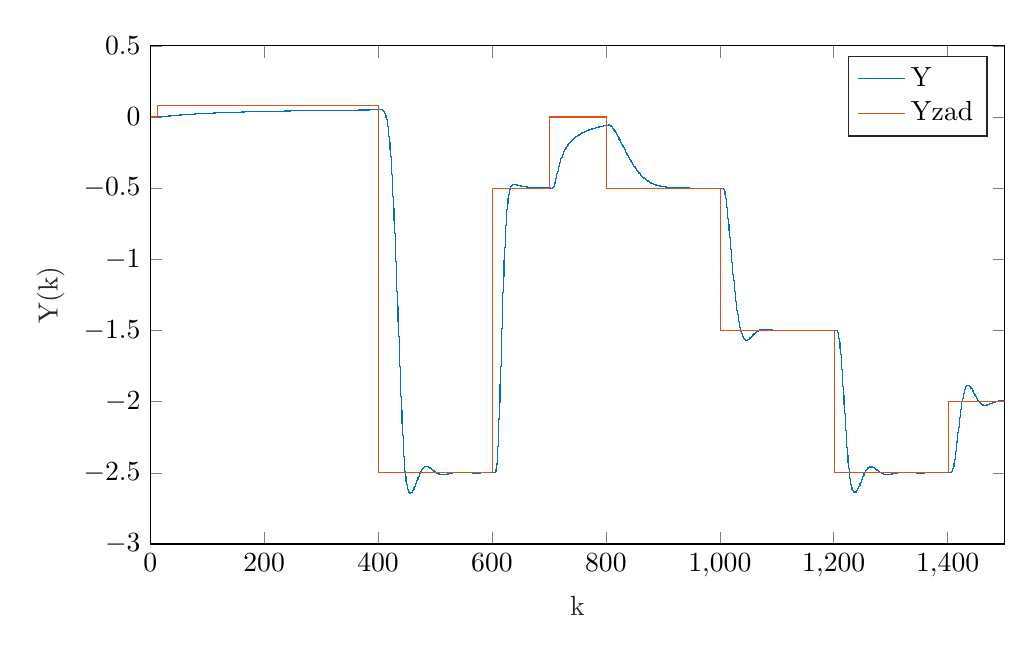
\begin{tikzpicture}

\begin{axis}[%
width=4.272in,
height=2.491in,
at={(0.717in,0.423in)},
scale only axis,
xmin=0,
xmax=1500,
xlabel style={font=\color{white!15!black}},
xlabel={k},
ymin=-3,
ymax=0.5,
ylabel style={font=\color{white!15!black}},
ylabel={Y(k)},
axis background/.style={fill=white},
legend style={legend cell align=left, align=left, draw=white!15!black}
]
\addplot[const plot, color=mycolor1] table[row sep=crcr] {%
1	0\\
2	0\\
3	0\\
4	0\\
5	0\\
6	0\\
7	0\\
8	0\\
9	0\\
10	0\\
11	0\\
12	0\\
13	0\\
14	0\\
15	0\\
16	0\\
17	6.52280482685478e-05\\
18	0.00025493947825112\\
19	0.000561156000357608\\
20	0.000952296976838165\\
21	0.00139530774711537\\
22	0.00186437213682768\\
23	0.00234243862882932\\
24	0.00281968544597944\\
25	0.00329124156104541\\
26	0.00375518905144472\\
27	0.00421114595257749\\
28	0.00465939572025324\\
29	0.00510041938417467\\
30	0.00553468241144488\\
31	0.00596256264997011\\
32	0.00638434529065104\\
33	0.00680024259688928\\
34	0.00721041760758585\\
35	0.00761500356139486\\
36	0.00801411715369817\\
37	0.00840786645936602\\
38	0.00879635510398442\\
39	0.0091796841439158\\
40	0.00955795271817484\\
41	0.00993125813833665\\
42	0.0102996957827645\\
43	0.0106633589683029\\
44	0.0110223388636318\\
45	0.0113767244552975\\
46	0.0117266025565261\\
47	0.0120720578442453\\
48	0.0124131729117849\\
49	0.0127500283285506\\
50	0.0130827027014591\\
51	0.013411272735424\\
52	0.013735813291727\\
53	0.0140563974439448\\
54	0.0143730965314795\\
55	0.0146859802108813\\
56	0.0149951165051603\\
57	0.0153005718512633\\
58	0.0156024111458486\\
59	0.0159006977894634\\
60	0.0161954937292049\\
61	0.0164868594999349\\
62	0.0167748542641041\\
63	0.0170595358502435\\
64	0.0173409607901714\\
65	0.0176191843549672\\
66	0.0178942605897565\\
67	0.0181662423473543\\
68	0.018435181320809\\
69	0.0187011280748886\\
70	0.0189641320765488\\
71	0.0192242417244214\\
72	0.0194815043773601\\
73	0.0197359663820766\\
74	0.0199876730999037\\
75	0.0202366689327144\\
76	0.0204829973480296\\
77	0.0207267009033435\\
78	0.0209678212696946\\
79	0.0212063992545095\\
80	0.0214424748237464\\
81	0.0216760871233612\\
82	0.021907274500123\\
83	0.0221360745217989\\
84	0.0223625239967323\\
85	0.0225866589928356\\
86	0.0228085148560163\\
87	0.0230281262280577\\
88	0.0232455270639719\\
89	0.0234607506488434\\
90	0.0236738296141813\\
91	0.0238847959537948\\
92	0.0240936810392111\\
93	0.0243005156346478\\
94	0.0245053299115574\\
95	0.0247081534627561\\
96	0.0249090153161518\\
97	0.0251079439480844\\
98	0.0253049672962903\\
99	0.0255001127725043\\
100	0.0256934072747107\\
101	0.0258848771990531\\
102	0.0260745484514173\\
103	0.026262446458694\\
104	0.0264485961797341\\
105	0.0266330221160057\\
106	0.0268157483219614\\
107	0.0269967984151263\\
108	0.0271761955859143\\
109	0.0273539626071818\\
110	0.0275301218435273\\
111	0.0277046952603434\\
112	0.0278777044326304\\
113	0.0280491705535776\\
114	0.0282191144429204\\
115	0.028387556555079\\
116	0.0285545169870857\\
117	0.0287200154863079\\
118	0.0288840714579716\\
119	0.0290467039724924\\
120	0.029207931772619\\
121	0.0293677732803955\\
122	0.0295262466039473\\
123	0.0296833695440956\\
124	0.0298391596008064\\
125	0.0299936339794775\\
126	0.0301468095970698\\
127	0.030298703088086\\
128	0.0304493308104012\\
129	0.0305987088509515\\
130	0.0307468530312816\\
131	0.0308937789129579\\
132	0.0310395018028499\\
133	0.0311840367582837\\
134	0.0313273985920713\\
135	0.0314696018774188\\
136	0.0316106609527175\\
137	0.0317505899262209\\
138	0.0318894026806103\\
139	0.0320271128774526\\
140	0.0321637339615535\\
141	0.0322992791652078\\
142	0.0324337615123511\\
143	0.0325671938226142\\
144	0.0326995887152841\\
145	0.0328309586131728\\
146	0.0329613157463977\\
147	0.0330906721560746\\
148	0.033219039697927\\
149	0.0333464300458131\\
150	0.033472854695172\\
151	0.0335983249663934\\
152	0.0337228520081105\\
153	0.0338464468004192\\
154	0.0339691201580256\\
155	0.0340908827333235\\
156	0.0342117450194029\\
157	0.034331717352993\\
158	0.0344508099173399\\
159	0.0345690327450212\\
160	0.0346863957206988\\
161	0.0348029085838121\\
162	0.0349185809312131\\
163	0.0350334222197432\\
164	0.0351474417687562\\
165	0.0352606487625852\\
166	0.0353730522529588\\
167	0.0354846611613638\\
168	0.0355954842813589\\
169	0.0357055302808392\\
170	0.0358148077042526\\
171	0.0359233249747695\\
172	0.0360310903964079\\
173	0.0361381121561128\\
174	0.0362443983257936\\
175	0.0363499568643181\\
176	0.0364547956194661\\
177	0.0365589223298424\\
178	0.0366623446267504\\
179	0.0367650700360277\\
180	0.0368671059798439\\
181	0.0369684597784624\\
182	0.0370691386519653\\
183	0.0371691497219452\\
184	0.0372685000131613\\
185	0.0373671964551635\\
186	0.0374652458838831\\
187	0.0375626550431927\\
188	0.0376594305864339\\
189	0.0377555790779164\\
190	0.0378511069943855\\
191	0.037946020726463\\
192	0.0380403265800575\\
193	0.0381340307777492\\
194	0.0382271394601462\\
195	0.0383196586872154\\
196	0.0384115944395869\\
197	0.0385029526198343\\
198	0.0385937390537288\\
199	0.038683959491471\\
200	0.0387736196088975\\
201	0.0388627250086659\\
202	0.0389512812214162\\
203	0.0390392937069112\\
204	0.0391267678551542\\
205	0.0392137089874869\\
206	0.0393001223576658\\
207	0.0393860131529186\\
208	0.0394713864949816\\
209	0.0395562474411168\\
210	0.0396406009851108\\
211	0.039724452058255\\
212	0.039807805530308\\
213	0.0398906662104399\\
214	0.0399730388481598\\
215	0.0400549281342257\\
216	0.0401363387015387\\
217	0.0402172751260203\\
218	0.0402977419274738\\
219	0.040377743570431\\
220	0.0404572844649825\\
221	0.040536368967594\\
222	0.0406150013819074\\
223	0.0406931859595284\\
224	0.040770926900799\\
225	0.0408482283555573\\
226	0.0409250944238835\\
227	0.0410015291568323\\
228	0.0410775365571534\\
229	0.0411531205799985\\
230	0.0412282851336165\\
231	0.0413030340800362\\
232	0.0413773712357372\\
233	0.0414513003723099\\
234	0.0415248252171027\\
235	0.0415979494538594\\
236	0.0416706767233449\\
237	0.0417430106239606\\
238	0.0418149547123485\\
239	0.0418865125039865\\
240	0.0419576874737717\\
241	0.0420284830565958\\
242	0.042098902647909\\
243	0.0421689496042753\\
244	0.042238627243919\\
245	0.0423079388472606\\
246	0.0423768876574451\\
247	0.0424454768808606\\
248	0.0425137096876491\\
249	0.0425815892122081\\
250	0.042649118553684\\
251	0.0427163007764581\\
252	0.0427831389106236\\
253	0.0428496359524556\\
254	0.042915794864873\\
255	0.0429816185778929\\
256	0.0430471099890777\\
257	0.043112271963975\\
258	0.0431771073365504\\
259	0.0432416189096129\\
260	0.0433058094552343\\
261	0.0433696817151609\\
262	0.0434332384012194\\
263	0.043496482195716\\
264	0.043559415751829\\
265	0.0436220416939954\\
266	0.0436843626182913\\
267	0.0437463810928066\\
268	0.043808099658013\\
269	0.0438695208271272\\
270	0.0439306470864675\\
271	0.0439914808958056\\
272	0.0440520246887126\\
273	0.0441122808728994\\
274	0.0441722518305521\\
275	0.0442319399186622\\
276	0.0442913474693516\\
277	0.0443504767901929\\
278	0.0444093301645239\\
279	0.0444679098517586\\
280	0.0445262180876924\\
281	0.0445842570848032\\
282	0.0446420290325477\\
283	0.0446995360976531\\
284	0.0447567804244047\\
285	0.0448137641349291\\
286	0.0448704893294728\\
287	0.0449269580866771\\
288	0.0449831724638486\\
289	0.0450391344972256\\
290	0.0450948462022408\\
291	0.0451503095737798\\
292	0.0452055265864363\\
293	0.0452604991947624\\
294	0.0453152293335168\\
295	0.045369718917908\\
296	0.0454239698438345\\
297	0.0454779839881215\\
298	0.0455317632087539\\
299	0.0455853093451065\\
300	0.0456386242181698\\
301	0.0456917096307737\\
302	0.0457445673678069\\
303	0.0457971991964342\\
304	0.0458496068663097\\
305	0.0459017921097874\\
306	0.0459537566421291\\
307	0.0460055021617083\\
308	0.0460570303502126\\
309	0.0461083428728419\\
310	0.0461594413785048\\
311	0.0462103275000114\\
312	0.0462610028542641\\
313	0.046311469042445\\
314	0.0463617276502016\\
315	0.0464117802478286\\
316	0.0464616283904487\\
317	0.0465112736181893\\
318	0.0465607174563581\\
319	0.0466099614156152\\
320	0.0466590069921437\\
321	0.0467078556678173\\
322	0.0467565089103658\\
323	0.0468049681735382\\
324	0.046853234897264\\
325	0.046901310507812\\
326	0.0469491964179463\\
327	0.0469968940270815\\
328	0.0470444047214347\\
329	0.0470917298741758\\
330	0.0471388708455758\\
331	0.0471858289831532\\
332	0.0472326056218181\\
333	0.0472792020840146\\
334	0.0473256196798611\\
335	0.0473718597072891\\
336	0.0474179234521798\\
337	0.0474638121884989\\
338	0.0475095271784296\\
339	0.0475550696725042\\
340	0.0476004409097333\\
341	0.0476456421177339\\
342	0.0476906745128558\\
343	0.0477355393003053\\
344	0.0477802376742689\\
345	0.0478247708180342\\
346	0.0478691399041096\\
347	0.0479133460943425\\
348	0.0479573905400356\\
349	0.0480012743820623\\
350	0.0480449987509803\\
351	0.0480885647671431\\
352	0.0481319735408114\\
353	0.0481752261722619\\
354	0.0482183237518953\\
355	0.0482612673603425\\
356	0.04830405806857\\
357	0.0483466969379833\\
358	0.0483891850205296\\
359	0.0484315233587989\\
360	0.0484737129861233\\
361	0.0485157549266764\\
362	0.0485576501955699\\
363	0.0485993997989503\\
364	0.0486410047340929\\
365	0.0486824659894967\\
366	0.0487237845449757\\
367	0.0487649613717512\\
368	0.0488059974325413\\
369	0.0488468936816506\\
370	0.0488876510650578\\
371	0.0489282705205025\\
372	0.0489687529775714\\
373	0.049009099357783\\
374	0.0490493105746709\\
375	0.0490893875338669\\
376	0.0491293311331825\\
377	0.0491691422626897\\
378	0.0492088218048006\\
379	0.0492483706343458\\
380	0.0492877896186528\\
381	0.0493270796176222\\
382	0.0493662414838041\\
383	0.0494052760624725\\
384	0.0494441841916998\\
385	0.0494829667024298\\
386	0.0495216244185499\\
387	0.0495601581569626\\
388	0.0495985687276561\\
389	0.0496368569337739\\
390	0.0496750235716838\\
391	0.0497130694310458\\
392	0.0497509952948796\\
393	0.0497888019396309\\
394	0.0498264901352367\\
395	0.0498640606451911\\
396	0.0499015142266086\\
397	0.0499388516302877\\
398	0.0499760736007737\\
399	0.0500131808764206\\
400	0.0500501741894518\\
401	0.0500870542660213\\
402	0.0501238218262728\\
403	0.050160477584399\\
404	0.0501970222487002\\
405	0.0502334565216415\\
406	0.0502304872867085\\
407	0.049060720021633\\
408	0.0465824433634822\\
409	0.0428045476549301\\
410	0.0376442871078276\\
411	0.0308821905445889\\
412	0.022174610920014\\
413	0.0110809476595657\\
414	-0.00290712643128221\\
415	-0.0203365755172202\\
416	-0.0417639244903633\\
417	-0.0677265355764118\\
418	-0.0987154616705655\\
419	-0.135151593422065\\
420	-0.177366747073491\\
421	-0.225590814990224\\
422	-0.279945335215457\\
423	-0.340443066247454\\
424	-0.406992537851354\\
425	-0.479406193254183\\
426	-0.557410658773615\\
427	-0.640657824725944\\
428	-0.728735716868028\\
429	-0.821178494661667\\
430	-0.917475258584464\\
431	-1.01707763424691\\
432	-1.11940630196771\\
433	-1.2238567534659\\
434	-1.3298045935455\\
435	-1.43661068268646\\
436	-1.54362635690164\\
437	-1.65019888292258\\
438	-1.75567722486287\\
439	-1.85941812372918\\
440	-1.9607924300878\\
441	-2.05919158591216\\
442	-2.15285715127687\\
443	-2.23909679774519\\
444	-2.31606924001544\\
445	-2.38304512169116\\
446	-2.44005924001663\\
447	-2.48764411298408\\
448	-2.52663035134281\\
449	-2.55800091425686\\
450	-2.58278804504292\\
451	-2.60200337953105\\
452	-2.61659331480538\\
453	-2.62732353782411\\
454	-2.63476280241189\\
455	-2.63933952335349\\
456	-2.64139303181487\\
457	-2.64120772473294\\
458	-2.63903487603003\\
459	-2.63510604094513\\
460	-2.62964089624352\\
461	-2.6228514409489\\
462	-2.61494384413453\\
463	-2.6061188014204\\
464	-2.5965709803828\\
465	-2.5864879481858\\
466	-2.57604884959183\\
467	-2.56542301861505\\
468	-2.55476864851237\\
469	-2.54423160355778\\
470	-2.53394442631831\\
471	-2.52402557222721\\
472	-2.51457888676075\\
473	-2.50569332796193\\
474	-2.49744292746037\\
475	-2.48988697589032\\
476	-2.48307041329352\\
477	-2.47702440140869\\
478	-2.47176705245664\\
479	-2.46730428792346\\
480	-2.46363080073155\\
481	-2.46073109488879\\
482	-2.45858057804443\\
483	-2.45714668419374\\
484	-2.45639000591187\\
485	-2.45626541782757\\
486	-2.45672317545621\\
487	-2.45770997590582\\
488	-2.45916996927672\\
489	-2.46104571174312\\
490	-2.46327905329824\\
491	-2.46581195494373\\
492	-2.46858723170346\\
493	-2.47154921924299\\
494	-2.47464436309114\\
495	-2.47782173050302\\
496	-2.48103344589293\\
497	-2.48423505151939\\
498	-2.48738579574159\\
499	-2.49044885170382\\
500	-2.49339146975662\\
501	-2.49618506730367\\
502	-2.49880526008171\\
503	-2.50123183914522\\
504	-2.50344869804322\\
505	-2.50544371484682\\
506	-2.50720859381488\\
507	-2.50873867157214\\
508	-2.51003269271964\\
509	-2.51109255980118\\
510	-2.51192306251056\\
511	-2.51253159094333\\
512	-2.51292783757224\\
513	-2.51312349245949\\
514	-2.51313193601188\\
515	-2.51296793333892\\
516	-2.51264733399289\\
517	-2.51218678055604\\
518	-2.5116034291997\\
519	-2.51091468497668\\
520	-2.51013795422882\\
521	-2.50929041610142\\
522	-2.50838881476148\\
523	-2.50744927352395\\
524	-2.5064871317053\\
525	-2.50551680465203\\
526	-2.50455166703891\\
527	-2.50360395920247\\
528	-2.50268471597227\\
529	-2.50180371719093\\
530	-2.50096945887383\\
531	-2.5001891437543\\
532	-2.49946868978942\\
533	-2.49881275506595\\
534	-2.49822477744436\\
535	-2.49770702721046\\
536	-2.49726067096697\\
537	-2.49688584498852\\
538	-2.49658173628228\\
539	-2.49634666963768\\
540	-2.49617819901158\\
541	-2.49607320167578\\
542	-2.49602797364901\\
543	-2.49603832504331\\
544	-2.49609967407143\\
545	-2.49620713858555\\
546	-2.49635562414549\\
547	-2.49653990774471\\
548	-2.49675471645254\\
549	-2.49699480035975\\
550	-2.49725499933977\\
551	-2.49753030325898\\
552	-2.49781590538454\\
553	-2.49810724884694\\
554	-2.49840006611567\\
555	-2.49869041153977\\
556	-2.49897468708981\\
557	-2.49924966151416\\
558	-2.49951248318953\\
559	-2.49976068700408\\
560	-2.49999219566092\\
561	-2.50020531583002\\
562	-2.50039872960888\\
563	-2.50057148177574\\
564	-2.50072296333476\\
565	-2.50085289186111\\
566	-2.50096128915462\\
567	-2.50104845670559\\
568	-2.5011149494649\\
569	-2.50116154839371\\
570	-2.50118923224663\\
571	-2.5011991490166\\
572	-2.50119258744026\\
573	-2.5011709489309\\
574	-2.50113572027128\\
575	-2.50108844736293\\
576	-2.50103071029123\\
577	-2.50096409992806\\
578	-2.50089019625621\\
579	-2.50081054856261\\
580	-2.5007266576115\\
581	-2.50063995987354\\
582	-2.50055181385431\\
583	-2.50046348853422\\
584	-2.50037615390334\\
585	-2.50029087354837\\
586	-2.50020859922536\\
587	-2.50013016733099\\
588	-2.50005629716704\\
589	-2.49998759087771\\
590	-2.49992453492691\\
591	-2.49986750297288\\
592	-2.49981675999096\\
593	-2.49977246749022\\
594	-2.4997346896683\\
595	-2.49970340034847\\
596	-2.49967849054537\\
597	-2.49965977651003\\
598	-2.49964700811019\\
599	-2.49963987740939\\
600	-2.49963802731654\\
601	-2.49964106018699\\
602	-2.4996485462664\\
603	-2.49966003187949\\
604	-2.49967504727698\\
605	-2.49969311406521\\
606	-2.49313073047323\\
607	-2.47370906867715\\
608	-2.43788853128489\\
609	-2.38419973241066\\
610	-2.3126997849974\\
611	-2.22455574505104\\
612	-2.12173789740072\\
613	-2.00678872813671\\
614	-1.88263673597516\\
615	-1.75243372153186\\
616	-1.61940313941603\\
617	-1.48669450623019\\
618	-1.35724491738724\\
619	-1.23365343045346\\
620	-1.11807700224664\\
621	-1.0121572459335\\
622	-0.916985225205362\\
623	-0.833107192953889\\
624	-0.760568725748036\\
625	-0.698989561242056\\
626	-0.647657943616953\\
627	-0.605632141391708\\
628	-0.571837963565968\\
629	-0.545153890380695\\
630	-0.524478915439747\\
631	-0.508781510523341\\
632	-0.497130712099043\\
633	-0.48871197044135\\
634	-0.482831150616355\\
635	-0.478910134804425\\
636	-0.476477098052503\\
637	-0.475153938692053\\
638	-0.47464270540939\\
639	-0.474712277098954\\
640	-0.475186068683421\\
641	-0.475931169290974\\
642	-0.476849060422995\\
643	-0.477867892849712\\
644	-0.478936201062705\\
645	-0.480017883732388\\
646	-0.481088261567528\\
647	-0.482131027772429\\
648	-0.483135921904127\\
649	-0.484096979153866\\
650	-0.485011229914205\\
651	-0.485877746540763\\
652	-0.486696954176018\\
653	-0.487470139800569\\
654	-0.488199108197397\\
655	-0.488885945402614\\
656	-0.489532859752205\\
657	-0.490142078151882\\
658	-0.490715781033509\\
659	-0.491256063930022\\
660	-0.491764916977637\\
661	-0.492244216174329\\
662	-0.49269572208114\\
663	-0.493121083004848\\
664	-0.493521840671676\\
665	-0.493899437089325\\
666	-0.494255221773888\\
667	-0.494590458846225\\
668	-0.494906333721983\\
669	-0.495203959262622\\
670	-0.495484381344731\\
671	-0.495748583858638\\
672	-0.495997493176805\\
673	-0.496231982146374\\
674	-0.496452873664233\\
675	-0.496660943891285\\
676	-0.496856925157729\\
677	-0.497041508604938\\
678	-0.497215346602902\\
679	-0.497379054975933\\
680	-0.4975332150636\\
681	-0.497678375638925\\
682	-0.497815054701696\\
683	-0.497943741161301\\
684	-0.498064896420701\\
685	-0.498178955870936\\
686	-0.498286330303807\\
687	-0.498387407249016\\
688	-0.498482552240991\\
689	-0.498572110019843\\
690	-0.498656405670257\\
691	-0.498735745701692\\
692	-0.498810419072892\\
693	-0.498880698163452\\
694	-0.498946839694974\\
695	-0.499009085604192\\
696	-0.499067663870308\\
697	-0.499122789298674\\
698	-0.499174664262868\\
699	-0.499223479407134\\
700	-0.499269414311059\\
701	-0.49931263811832\\
702	-0.49935331013124\\
703	-0.499391580372846\\
704	-0.499427590118039\\
705	-0.499461472395446\\
706	-0.498003779244285\\
707	-0.493873617565184\\
708	-0.486681931709205\\
709	-0.476553195728536\\
710	-0.463907256735659\\
711	-0.449302195738835\\
712	-0.433329759748204\\
713	-0.416550362524102\\
714	-0.399456126986195\\
715	-0.382453306609721\\
716	-0.365857818790035\\
717	-0.349899336528318\\
718	-0.334730584498857\\
719	-0.320439356732259\\
720	-0.307061443154506\\
721	-0.294593192394263\\
722	-0.283002882583514\\
723	-0.272240430980255\\
724	-0.262245255990424\\
725	-0.252952312484039\\
726	-0.24429645992843\\
727	-0.236215402853667\\
728	-0.228651476187157\\
729	-0.221552546453217\\
730	-0.214872275474905\\
731	-0.208569956123501\\
732	-0.202610087734169\\
733	-0.196961817656716\\
734	-0.191598338565245\\
735	-0.186496300425325\\
736	-0.181635271950952\\
737	-0.176997268657059\\
738	-0.172566352407471\\
739	-0.168328299630387\\
740	-0.164270331051886\\
741	-0.160380893903539\\
742	-0.156649487270538\\
743	-0.153066521917404\\
744	-0.149623207087119\\
745	-0.146311458094034\\
746	-0.14312381981959\\
747	-0.140053402362157\\
748	-0.137093826040973\\
749	-0.134239173703283\\
750	-0.131483948850907\\
751	-0.128823038516478\\
752	-0.12625168011244\\
753	-0.123765431677444\\
754	-0.121360145080816\\
755	-0.11903194183663\\
756	-0.116777191239904\\
757	-0.114592490579571\\
758	-0.112474647213385\\
759	-0.110420662313666\\
760	-0.10842771611247\\
761	-0.106493154492084\\
762	-0.104614476782368\\
763	-0.102789324640869\\
764	-0.101015471904821\\
765	-0.099290815316249\\
766	-0.0976133660323043\\
767	-0.09598124184282\\
768	-0.0943926600258109\\
769	-0.0928459307793967\\
770	-0.091339451175459\\
771	-0.0898716995863341\\
772	-0.0884412305411095\\
773	-0.0870466699727056\\
774	-0.0856867108209803\\
775	-0.0843601089606619\\
776	-0.0830656794260634\\
777	-0.081802292907315\\
778	-0.0805688724953162\\
779	-0.0793643906548071\\
780	-0.0781878664069061\\
781	-0.0770383627042094\\
782	-0.0759149839831064\\
783	-0.0748168738793606\\
784	-0.0737432130942646\\
785	-0.0726932173998002\\
786	-0.0716661357722542\\
787	-0.0706612486446516\\
788	-0.0696778662691969\\
789	-0.0687153271816563\\
790	-0.0677729967602951\\
791	-0.0668502658725872\\
792	-0.0659465496034787\\
793	-0.0650612860594809\\
794	-0.0641939352433346\\
795	-0.0633439779943983\\
796	-0.0625109149902956\\
797	-0.0616942658057014\\
798	-0.0608935680244644\\
799	-0.0601083764015495\\
800	-0.0593382620715517\\
801	-0.0585828118007698\\
802	-0.0578416272800557\\
803	-0.0571143244558526\\
804	-0.0564005328970268\\
805	-0.0556998951952664\\
806	-0.0557387550090958\\
807	-0.0570791707494993\\
808	-0.0597533646996517\\
809	-0.0635619984906342\\
810	-0.0682446597070543\\
811	-0.073563123811276\\
812	-0.0793314119750974\\
813	-0.0854180775615016\\
814	-0.0917368908035845\\
815	-0.0982346567299622\\
816	-0.104880161383628\\
817	-0.111655605381192\\
818	-0.118550598356063\\
819	-0.125558273832576\\
820	-0.132672965108801\\
821	-0.139888938486547\\
822	-0.147199792977308\\
823	-0.154598251512996\\
824	-0.162076162835341\\
825	-0.169624602888493\\
826	-0.177234012357986\\
827	-0.184894337447724\\
828	-0.192595159140574\\
829	-0.200325806216348\\
830	-0.208075452285036\\
831	-0.215833199145724\\
832	-0.223588149263085\\
833	-0.231329469888549\\
834	-0.239046450810578\\
835	-0.246728557141278\\
836	-0.25436547804558\\
837	-0.261947171930734\\
838	-0.269463908337567\\
839	-0.276906306593997\\
840	-0.284265371184654\\
841	-0.291532523738109\\
842	-0.298699631518272\\
843	-0.305759032316162\\
844	-0.312703555662933\\
845	-0.319526540318032\\
846	-0.326221848023244\\
847	-0.332783873550996\\
848	-0.3392075511119\\
849	-0.345488357220763\\
850	-0.351622310151609\\
851	-0.357605966140113\\
852	-0.363436412516133\\
853	-0.369111257969612\\
854	-0.374628620169997\\
855	-0.37998711097259\\
856	-0.38518581945498\\
857	-0.39022429303305\\
858	-0.395102516909172\\
859	-0.399820892105299\\
860	-0.404380212330934\\
861	-0.408781639930679\\
862	-0.413026681148402\\
863	-0.417117160935396\\
864	-0.421055197518401\\
865	-0.424843176930336\\
866	-0.428483727692371\\
867	-0.431979695820717\\
868	-0.435334120315596\\
869	-0.4385502092735\\
870	-0.441631316747235\\
871	-0.444580920461729\\
872	-0.447402600477204\\
873	-0.450100018875417\\
874	-0.452676900529313\\
875	-0.455137015001778\\
876	-0.457484159605403\\
877	-0.459722143642252\\
878	-0.461854773830771\\
879	-0.463885840916129\\
880	-0.465819107450523\\
881	-0.467658296721343\\
882	-0.469407082797482\\
883	-0.471069081657615\\
884	-0.472647843358773\\
885	-0.474146845199073\\
886	-0.475569485824929\\
887	-0.4769190802304\\
888	-0.478198855594487\\
889	-0.479411947901079\\
890	-0.480561399285808\\
891	-0.481650156054229\\
892	-0.482681067316421\\
893	-0.483656884184237\\
894	-0.484580259478955\\
895	-0.485453747898909\\
896	-0.486279806598797\\
897	-0.487060796134644\\
898	-0.487798981730881\\
899	-0.488496534828525\\
900	-0.489155534876101\\
901	-0.489777971327577\\
902	-0.490365745814233\\
903	-0.490920674459986\\
904	-0.491444490312248\\
905	-0.491938845862871\\
906	-0.492405315636093\\
907	-0.49284539882271\\
908	-0.493260521941797\\
909	-0.49365204151342\\
910	-0.494021246727615\\
911	-0.494369362096741\\
912	-0.494697550079967\\
913	-0.49500691367017\\
914	-0.495298498934939\\
915	-0.495573297504668\\
916	-0.495832249001894\\
917	-0.496076243407107\\
918	-0.496306123357197\\
919	-0.496522686373597\\
920	-0.496726687017919\\
921	-0.496918838973589\\
922	-0.497099817052568\\
923	-0.497270259126799\\
924	-0.497430767984461\\
925	-0.497581913111521\\
926	-0.497724232399429\\
927	-0.497858233780073\\
928	-0.49798439678937\\
929	-0.498103174061073\\
930	-0.49821499275254\\
931	-0.498320255904343\\
932	-0.498419343735701\\
933	-0.498512614877795\\
934	-0.498600407547099\\
935	-0.498683040660847\\
936	-0.498760814896843\\
937	-0.49883401369976\\
938	-0.498902904236093\\
939	-0.498967738299919\\
940	-0.499028753171555\\
941	-0.499086172431193\\
942	-0.499140206729534\\
943	-0.499191054517393\\
944	-0.499238902736192\\
945	-0.4992839274712\\
946	-0.499326294569331\\
947	-0.499366160223214\\
948	-0.499403671523239\\
949	-0.499438966979155\\
950	-0.499472177012805\\
951	-0.49950342442345\\
952	-0.499532824827113\\
953	-0.499560487071318\\
954	-0.49958651362649\\
955	-0.499611000955288\\
956	-0.499634039861034\\
957	-0.499655715816372\\
958	-0.499676109273222\\
959	-0.499695295955056\\
960	-0.499713347132464\\
961	-0.499730329882929\\
962	-0.499746307335681\\
963	-0.499761338902468\\
964	-0.499775480495023\\
965	-0.499788784729976\\
966	-0.499801301121919\\
967	-0.499813076265281\\
968	-0.499824154005662\\
969	-0.499834575601214\\
970	-0.499844379874635\\
971	-0.499853603356321\\
972	-0.499862280419164\\
973	-0.499870443405498\\
974	-0.499878122746622\\
975	-0.499885347075339\\
976	-0.499892143331917\\
977	-0.499898536863835\\
978	-0.499904551519695\\
979	-0.499910209737621\\
980	-0.499915532628473\\
981	-0.499920540054175\\
982	-0.499925250701442\\
983	-0.499929682151173\\
984	-0.499933850943765\\
985	-0.499937772640578\\
986	-0.499941461881787\\
987	-0.499944932440829\\
988	-0.499948197275634\\
989	-0.499951268576844\\
990	-0.499954157813186\\
991	-0.499956875774167\\
992	-0.499959432610256\\
993	-0.499961837870688\\
994	-0.499964100539039\\
995	-0.499966229066703\\
996	-0.499968231404384\\
997	-0.499970115031738\\
998	-0.499971886985255\\
999	-0.499973553884497\\
1000	-0.499975121956784\\
1001	-0.499976597060418\\
1002	-0.499977984706542\\
1003	-0.499979290079693\\
1004	-0.499980518057152\\
1005	-0.49998167322714\\
1006	-0.502900966663938\\
1007	-0.511036716078179\\
1008	-0.525223464315934\\
1009	-0.545416862831597\\
1010	-0.571101377956774\\
1011	-0.601551567893476\\
1012	-0.635984624642048\\
1013	-0.67364130361582\\
1014	-0.713823394504983\\
1015	-0.755906492837597\\
1016	-0.799339775304321\\
1017	-0.843639734995405\\
1018	-0.888381807095623\\
1019	-0.933191959860361\\
1020	-0.977739228435644\\
1021	-1.0217295477961\\
1022	-1.06490090870257\\
1023	-1.10701970320061\\
1024	-1.14787806129941\\
1025	-1.1872919688398\\
1026	-1.22509997150295\\
1027	-1.26116229541418\\
1028	-1.29536024292126\\
1029	-1.32759574894817\\
1030	-1.35779100719855\\
1031	-1.38588809597168\\
1032	-1.41184855061862\\
1033	-1.43565284411381\\
1034	-1.45729974931388\\
1035	-1.47680556665681\\
1036	-1.4942032096823\\
1037	-1.50954114810986\\
1038	-1.52288221449654\\
1039	-1.53430228584579\\
1040	-1.54388885603331\\
1041	-1.55173951859562\\
1042	-1.55796038230472\\
1043	-1.56266444402835\\
1044	-1.56596994464298\\
1045	-1.56799873422948\\
1046	-1.56887467245045\\
1047	-1.5687220889197\\
1048	-1.56766432657991\\
1049	-1.56582238868459\\
1050	-1.56331370703282\\
1051	-1.5602510457486\\
1052	-1.5567415512631\\
1053	-1.55288595538561\\
1054	-1.54877793457736\\
1055	-1.54450362490525\\
1056	-1.54014128876806\\
1057	-1.53576112645902\\
1058	-1.53142522303336\\
1059	-1.52718761884195\\
1060	-1.52309449050054\\
1061	-1.51918442799221\\
1062	-1.51548879302874\\
1063	-1.51203214368877\\
1064	-1.50883271065266\\
1065	-1.50590291100493\\
1066	-1.50324988650698\\
1067	-1.50087605438483\\
1068	-1.49877965996409\\
1069	-1.49695532185211\\
1070	-1.49539456176334\\
1071	-1.49408631245897\\
1072	-1.49301739859056\\
1073	-1.49217298646958\\
1074	-1.49153699991102\\
1075	-1.49109250030756\\
1076	-1.49082202997432\\
1077	-1.49070791856366\\
1078	-1.49073255298826\\
1079	-1.49087861181534\\
1080	-1.49112926551573\\
1081	-1.49146834427745\\
1082	-1.49188047533661\\
1083	-1.49235119194898\\
1084	-1.4928670162343\\
1085	-1.49341551818199\\
1086	-1.49398535311991\\
1087	-1.49456627992596\\
1088	-1.49514916221085\\
1089	-1.49572595462771\\
1090	-1.49628967637223\\
1091	-1.49683437383331\\
1092	-1.49735507423939\\
1093	-1.49784773202433\\
1094	-1.49830916951139\\
1095	-1.49873701338483\\
1096	-1.49912962829027\\
1097	-1.49948604877579\\
1098	-1.49980591065929\\
1099	-1.50008938278337\\
1100	-1.50033709999878\\
1101	-1.50055009810106\\
1102	-1.50072975133442\\
1103	-1.500877712971\\
1104	-1.50099585937468\\
1105	-1.50108623786529\\
1106	-1.50115101861315\\
1107	-1.50119245071473\\
1108	-1.50121282252791\\
1109	-1.50121442628089\\
1110	-1.50119952691111\\
1111	-1.50117033504005\\
1112	-1.50112898394661\\
1113	-1.5010775103649\\
1114	-1.50101783890254\\
1115	-1.5009517698513\\
1116	-1.50088097014406\\
1117	-1.50080696719934\\
1118	-1.50073114538683\\
1119	-1.5006547448443\\
1120	-1.50057886237672\\
1121	-1.50050445417326\\
1122	-1.50043234008465\\
1123	-1.50036320921401\\
1124	-1.50029762658586\\
1125	-1.50023604067243\\
1126	-1.5001787915713\\
1127	-1.50012611964484\\
1128	-1.50007817444853\\
1129	-1.50003502379267\\
1130	-1.4999966627989\\
1131	-1.49996302283011\\
1132	-1.49993398018881\\
1133	-1.49990936449495\\
1134	-1.49988896666942\\
1135	-1.49987254646396\\
1136	-1.49985983949129\\
1137	-1.49985056372197\\
1138	-1.49984442542564\\
1139	-1.49984112454448\\
1140	-1.49984035949611\\
1141	-1.49984183141084\\
1142	-1.49984524781551\\
1143	-1.49985032578186\\
1144	-1.49985679456265\\
1145	-1.49986439774247\\
1146	-1.49987289493371\\
1147	-1.49988206305042\\
1148	-1.49989169719445\\
1149	-1.49990161118921\\
1150	-1.49991163779702\\
1151	-1.49992162865565\\
1152	-1.49993145396916\\
1153	-1.49994100198718\\
1154	-1.49995017830537\\
1155	-1.4999589050184\\
1156	-1.49996711975457\\
1157	-1.49997477461969\\
1158	-1.4999818350753\\
1159	-1.49998827877434\\
1160	-1.49999409437511\\
1161	-1.49999928035204\\
1162	-1.50000384381966\\
1163	-1.50000779938389\\
1164	-1.50001116803279\\
1165	-1.50001397607682\\
1166	-1.50001625414686\\
1167	-1.50001803625623\\
1168	-1.50001935893179\\
1169	-1.50002026041705\\
1170	-1.50002077994941\\
1171	-1.50002095711221\\
1172	-1.50002083126101\\
1173	-1.5000204410229\\
1174	-1.50001982386665\\
1175	-1.50001901574076\\
1176	-1.50001805077605\\
1177	-1.50001696104891\\
1178	-1.50001577640104\\
1179	-1.50001452431107\\
1180	-1.50001322981367\\
1181	-1.50001191546126\\
1182	-1.50001060132376\\
1183	-1.50000930502167\\
1184	-1.50000804178809\\
1185	-1.50000682455511\\
1186	-1.50000566406072\\
1187	-1.500004568972\\
1188	-1.50000354602123\\
1189	-1.50000260015134\\
1190	-1.5000017346676\\
1191	-1.50000095139294\\
1192	-1.50000025082413\\
1193	-1.49999963228675\\
1194	-1.49999909408707\\
1195	-1.499998633659\\
1196	-1.49999824770492\\
1197	-1.49999793232914\\
1198	-1.49999768316308\\
1199	-1.49999749548163\\
1200	-1.49999736431001\\
1201	-1.49999728452107\\
1202	-1.49999725092266\\
1203	-1.49999725833529\\
1204	-1.49999730166017\\
1205	-1.49999737593778\\
1206	-1.50319698465028\\
1207	-1.51238541909091\\
1208	-1.52891775562384\\
1209	-1.5531846267003\\
1210	-1.58496490805612\\
1211	-1.62367351773443\\
1212	-1.66852503753065\\
1213	-1.71863779164015\\
1214	-1.77309840068139\\
1215	-1.83100083034788\\
1216	-1.89146928108416\\
1217	-1.9536710395795\\
1218	-2.01682325913131\\
1219	-2.08019620847338\\
1220	-2.14311458336265\\
1221	-2.20495785085989\\
1222	-2.2651601860319\\
1223	-2.32321029951256\\
1224	-2.377435815232\\
1225	-2.42640249442705\\
1226	-2.4694258833842\\
1227	-2.50636271316126\\
1228	-2.53743080050663\\
1229	-2.56307284537578\\
1230	-2.58385589204491\\
1231	-2.60039924717887\\
1232	-2.61330042974794\\
1233	-2.62302987436639\\
1234	-2.62994317215629\\
1235	-2.63432362654076\\
1236	-2.63641138054345\\
1237	-2.63642224236097\\
1238	-2.63455920097039\\
1239	-2.63101903908235\\
1240	-2.62599572239924\\
1241	-2.61968169310157\\
1242	-2.61226782540985\\
1243	-2.6039425554496\\
1244	-2.5948905348814\\
1245	-2.58529104912544\\
1246	-2.57531636751444\\
1247	-2.56513014201445\\
1248	-2.5548859353089\\
1249	-2.54472593295291\\
1250	-2.53477987473022\\
1251	-2.52516422524192\\
1252	-2.5159815918535\\
1253	-2.50732038864403\\
1254	-2.49925473745828\\
1255	-2.49184459126073\\
1256	-2.48513606052709\\
1257	-2.47916192023208\\
1258	-2.47394227296581\\
1259	-2.46948534270205\\
1260	-2.46578837361347\\
1261	-2.46283860893758\\
1262	-2.46061432610054\\
1263	-2.45908590596158\\
1264	-2.45821691601582\\
1265	-2.45796518956655\\
1266	-2.45828388514368\\
1267	-2.45912251271479\\
1268	-2.46042791543902\\
1269	-2.46214519779977\\
1270	-2.46421859288329\\
1271	-2.46659226332636\\
1272	-2.46921103202738\\
1273	-2.47202104010174\\
1274	-2.47497033077265\\
1275	-2.47800935893408\\
1276	-2.48109142701973\\
1277	-2.48417304857687\\
1278	-2.48721424159399\\
1279	-2.49017875418156\\
1280	-2.49303422567083\\
1281	-2.49575228658797\\
1282	-2.49830860129\\
1283	-2.50068285732367\\
1284	-2.5028587057925\\
1285	-2.50482365719683\\
1286	-2.50656893734751\\
1287	-2.50808930804823\\
1288	-2.50938285729431\\
1289	-2.51045076374712\\
1290	-2.51129704021333\\
1291	-2.51192826078568\\
1292	-2.51235327618881\\
1293	-2.51258292171838\\
1294	-2.51262972196809\\
1295	-2.51250759630664\\
1296	-2.51223156880063\\
1297	-2.51181748598132\\
1298	-2.51128174552843\\
1299	-2.51064103859799\\
1300	-2.5099121081574\\
1301	-2.50911152531723\\
1302	-2.50825548526999\\
1303	-2.50735962406764\\
1304	-2.50643885709847\\
1305	-2.50550723976409\\
1306	-2.50457785051518\\
1307	-2.50366269608382\\
1308	-2.50277263845468\\
1309	-2.5019173428507\\
1310	-2.50110524577268\\
1311	-2.5003435419284\\
1312	-2.49963818871686\\
1313	-2.49899392679583\\
1314	-2.49841431515696\\
1315	-2.49790177906036\\
1316	-2.49745766913823\\
1317	-2.49708232996337\\
1318	-2.4967751763899\\
1319	-2.49653477600891\\
1320	-2.49635893611732\\
1321	-2.49624479367156\\
1322	-2.49618890678624\\
1323	-2.49618734643834\\
1324	-2.49623578714779\\
1325	-2.49632959552232\\
1326	-2.49646391567647\\
1327	-2.49663375065901\\
1328	-2.49683403914802\\
1329	-2.49705972679691\\
1330	-2.49730583173561\\
1331	-2.49756750384866\\
1332	-2.49784007756353\\
1333	-2.49811911798886\\
1334	-2.49840046034092\\
1335	-2.49868024268825\\
1336	-2.49895493212792\\
1337	-2.49922134458212\\
1338	-2.49947665847005\\
1339	-2.49971842256872\\
1340	-2.49994455842504\\
1341	-2.50015335772294\\
1342	-2.5003434750416\\
1343	-2.50051391646539\\
1344	-2.50066402452307\\
1345	-2.50079345994297\\
1346	-2.50090218071374\\
1347	-2.5009904189361\\
1348	-2.50105865594168\\
1349	-2.5011075961396\\
1350	-2.50113814003205\\
1351	-2.50115135681614\\
1352	-2.5011484569617\\
1353	-2.50113076512483\\
1354	-2.50109969372395\\
1355	-2.50105671747096\\
1356	-2.50100334911484\\
1357	-2.50094111661845\\
1358	-2.50087154195366\\
1359	-2.50079612166376\\
1360	-2.50071630930737\\
1361	-2.50063349986438\\
1362	-2.50054901615207\\
1363	-2.5004640972697\\
1364	-2.50037988906146\\
1365	-2.50029743656204\\
1366	-2.5002176783658\\
1367	-2.50014144284008\\
1368	-2.5000694460849\\
1369	-2.50000229152656\\
1370	-2.49994047101978\\
1371	-2.4998843673234\\
1372	-2.49983425780726\\
1373	-2.49979031924324\\
1374	-2.49975263353081\\
1375	-2.49972119420721\\
1376	-2.49969591359419\\
1377	-2.49967663043657\\
1378	-2.4996631178932\\
1379	-2.49965509174743\\
1380	-2.49965221871187\\
1381	-2.49965412471127\\
1382	-2.49966040303672\\
1383	-2.49967062227471\\
1384	-2.49968433392552\\
1385	-2.49970107963577\\
1386	-2.4997203979818\\
1387	-2.49974183075068\\
1388	-2.4997649286773\\
1389	-2.49978925660572\\
1390	-2.49981439805353\\
1391	-2.49983995916723\\
1392	-2.49986557206557\\
1393	-2.49989089757618\\
1394	-2.49991562737816\\
1395	-2.49993948557\\
1396	-2.49996222968848\\
1397	-2.49998365120884\\
1398	-2.50000357556128\\
1399	-2.50002186170219\\
1400	-2.50003840128118\\
1401	-2.50005311744712\\
1402	-2.50006596333773\\
1403	-2.50007692029743\\
1404	-2.50008599586884\\
1405	-2.50009322160188\\
1406	-2.49847876498493\\
1407	-2.49373129702244\\
1408	-2.48502561264153\\
1409	-2.47203278389499\\
1410	-2.45476985884565\\
1411	-2.43348776061909\\
1412	-2.40859164257651\\
1413	-2.38058472137092\\
1414	-2.35002790887346\\
1415	-2.31750994099677\\
1416	-2.28362462095378\\
1417	-2.24895309653258\\
1418	-2.21404991779039\\
1419	-2.17943212619517\\
1420	-2.14557092139406\\
1421	-2.11288561292274\\
1422	-2.08173964169051\\
1423	-2.05243848051099\\
1424	-2.02522922192744\\
1425	-2.00030164737205\\
1426	-1.97779055514655\\
1427	-1.95777911296889\\
1428	-1.94030299743419\\
1429	-1.92535508889557\\
1430	-1.91289050547231\\
1431	-1.90283178249806\\
1432	-1.8950740314743\\
1433	-1.88948994306377\\
1434	-1.88593452956643\\
1435	-1.88424953176762\\
1436	-1.88426744162099\\
1437	-1.88581511503381\\
1438	-1.88871696763743\\
1439	-1.89279776082716\\
1440	-1.89788499581288\\
1441	-1.90381094039916\\
1442	-1.91041431727984\\
1443	-1.91754168438787\\
1444	-1.9250485378626\\
1445	-1.932800167004\\
1446	-1.94067228861727\\
1447	-1.94855148576947\\
1448	-1.95633547345591\\
1449	-1.96393321120603\\
1450	-1.9712648803803\\
1451	-1.97826174189962\\
1452	-1.98486588844497\\
1453	-1.99102990377197\\
1454	-1.9967164406865\\
1455	-2.00189772838916\\
1456	-2.00655501927825\\
1457	-2.0106779848554\\
1458	-2.01426407005872\\
1459	-2.01731781510977\\
1460	-2.01985015376134\\
1461	-2.02187769663665\\
1462	-2.02342200812602\\
1463	-2.02450888503085\\
1464	-2.02516764479849\\
1465	-2.02543043076457\\
1466	-2.02533154130651\\
1467	-2.02490678921386\\
1468	-2.02419289690403\\
1469	-2.02322693236585\\
1470	-2.02204578991243\\
1471	-2.02068571898501\\
1472	-2.01918190338926\\
1473	-2.0175680924838\\
1474	-2.01587628499588\\
1475	-2.01413646532921\\
1476	-2.01237639146994\\
1477	-2.01062143290257\\
1478	-2.00889445632933\\
1479	-2.00721575645309\\
1480	-2.0056030286397\\
1481	-2.00407137992466\\
1482	-2.00263337456945\\
1483	-2.00129911020322\\
1484	-2.00007632050019\\
1485	-1.99897050033581\\
1486	-1.99798504942752\\
1487	-1.99712143058985\\
1488	-1.99637933890944\\
1489	-1.99575687836408\\
1490	-1.99525074266114\\
1491	-1.99485639734704\\
1492	-1.99456826053117\\
1493	-1.99437987986893\\
1494	-1.99428410375149\\
1495	-1.99427324494976\\
1496	-1.99433923525195\\
1497	-1.9944737699138\\
1498	-1.99466844100561\\
1499	-1.99491485898808\\
1500	-1.99520476207818\\
};
\addlegendentry{Y}

\addplot[const plot, color=mycolor2] table[row sep=crcr] {%
1	0\\
2	0\\
3	0\\
4	0\\
5	0\\
6	0\\
7	0\\
8	0\\
9	0\\
10	0\\
11	0\\
12	0.08\\
13	0.08\\
14	0.08\\
15	0.08\\
16	0.08\\
17	0.08\\
18	0.08\\
19	0.08\\
20	0.08\\
21	0.08\\
22	0.08\\
23	0.08\\
24	0.08\\
25	0.08\\
26	0.08\\
27	0.08\\
28	0.08\\
29	0.08\\
30	0.08\\
31	0.08\\
32	0.08\\
33	0.08\\
34	0.08\\
35	0.08\\
36	0.08\\
37	0.08\\
38	0.08\\
39	0.08\\
40	0.08\\
41	0.08\\
42	0.08\\
43	0.08\\
44	0.08\\
45	0.08\\
46	0.08\\
47	0.08\\
48	0.08\\
49	0.08\\
50	0.08\\
51	0.08\\
52	0.08\\
53	0.08\\
54	0.08\\
55	0.08\\
56	0.08\\
57	0.08\\
58	0.08\\
59	0.08\\
60	0.08\\
61	0.08\\
62	0.08\\
63	0.08\\
64	0.08\\
65	0.08\\
66	0.08\\
67	0.08\\
68	0.08\\
69	0.08\\
70	0.08\\
71	0.08\\
72	0.08\\
73	0.08\\
74	0.08\\
75	0.08\\
76	0.08\\
77	0.08\\
78	0.08\\
79	0.08\\
80	0.08\\
81	0.08\\
82	0.08\\
83	0.08\\
84	0.08\\
85	0.08\\
86	0.08\\
87	0.08\\
88	0.08\\
89	0.08\\
90	0.08\\
91	0.08\\
92	0.08\\
93	0.08\\
94	0.08\\
95	0.08\\
96	0.08\\
97	0.08\\
98	0.08\\
99	0.08\\
100	0.08\\
101	0.08\\
102	0.08\\
103	0.08\\
104	0.08\\
105	0.08\\
106	0.08\\
107	0.08\\
108	0.08\\
109	0.08\\
110	0.08\\
111	0.08\\
112	0.08\\
113	0.08\\
114	0.08\\
115	0.08\\
116	0.08\\
117	0.08\\
118	0.08\\
119	0.08\\
120	0.08\\
121	0.08\\
122	0.08\\
123	0.08\\
124	0.08\\
125	0.08\\
126	0.08\\
127	0.08\\
128	0.08\\
129	0.08\\
130	0.08\\
131	0.08\\
132	0.08\\
133	0.08\\
134	0.08\\
135	0.08\\
136	0.08\\
137	0.08\\
138	0.08\\
139	0.08\\
140	0.08\\
141	0.08\\
142	0.08\\
143	0.08\\
144	0.08\\
145	0.08\\
146	0.08\\
147	0.08\\
148	0.08\\
149	0.08\\
150	0.08\\
151	0.08\\
152	0.08\\
153	0.08\\
154	0.08\\
155	0.08\\
156	0.08\\
157	0.08\\
158	0.08\\
159	0.08\\
160	0.08\\
161	0.08\\
162	0.08\\
163	0.08\\
164	0.08\\
165	0.08\\
166	0.08\\
167	0.08\\
168	0.08\\
169	0.08\\
170	0.08\\
171	0.08\\
172	0.08\\
173	0.08\\
174	0.08\\
175	0.08\\
176	0.08\\
177	0.08\\
178	0.08\\
179	0.08\\
180	0.08\\
181	0.08\\
182	0.08\\
183	0.08\\
184	0.08\\
185	0.08\\
186	0.08\\
187	0.08\\
188	0.08\\
189	0.08\\
190	0.08\\
191	0.08\\
192	0.08\\
193	0.08\\
194	0.08\\
195	0.08\\
196	0.08\\
197	0.08\\
198	0.08\\
199	0.08\\
200	0.08\\
201	0.08\\
202	0.08\\
203	0.08\\
204	0.08\\
205	0.08\\
206	0.08\\
207	0.08\\
208	0.08\\
209	0.08\\
210	0.08\\
211	0.08\\
212	0.08\\
213	0.08\\
214	0.08\\
215	0.08\\
216	0.08\\
217	0.08\\
218	0.08\\
219	0.08\\
220	0.08\\
221	0.08\\
222	0.08\\
223	0.08\\
224	0.08\\
225	0.08\\
226	0.08\\
227	0.08\\
228	0.08\\
229	0.08\\
230	0.08\\
231	0.08\\
232	0.08\\
233	0.08\\
234	0.08\\
235	0.08\\
236	0.08\\
237	0.08\\
238	0.08\\
239	0.08\\
240	0.08\\
241	0.08\\
242	0.08\\
243	0.08\\
244	0.08\\
245	0.08\\
246	0.08\\
247	0.08\\
248	0.08\\
249	0.08\\
250	0.08\\
251	0.08\\
252	0.08\\
253	0.08\\
254	0.08\\
255	0.08\\
256	0.08\\
257	0.08\\
258	0.08\\
259	0.08\\
260	0.08\\
261	0.08\\
262	0.08\\
263	0.08\\
264	0.08\\
265	0.08\\
266	0.08\\
267	0.08\\
268	0.08\\
269	0.08\\
270	0.08\\
271	0.08\\
272	0.08\\
273	0.08\\
274	0.08\\
275	0.08\\
276	0.08\\
277	0.08\\
278	0.08\\
279	0.08\\
280	0.08\\
281	0.08\\
282	0.08\\
283	0.08\\
284	0.08\\
285	0.08\\
286	0.08\\
287	0.08\\
288	0.08\\
289	0.08\\
290	0.08\\
291	0.08\\
292	0.08\\
293	0.08\\
294	0.08\\
295	0.08\\
296	0.08\\
297	0.08\\
298	0.08\\
299	0.08\\
300	0.08\\
301	0.08\\
302	0.08\\
303	0.08\\
304	0.08\\
305	0.08\\
306	0.08\\
307	0.08\\
308	0.08\\
309	0.08\\
310	0.08\\
311	0.08\\
312	0.08\\
313	0.08\\
314	0.08\\
315	0.08\\
316	0.08\\
317	0.08\\
318	0.08\\
319	0.08\\
320	0.08\\
321	0.08\\
322	0.08\\
323	0.08\\
324	0.08\\
325	0.08\\
326	0.08\\
327	0.08\\
328	0.08\\
329	0.08\\
330	0.08\\
331	0.08\\
332	0.08\\
333	0.08\\
334	0.08\\
335	0.08\\
336	0.08\\
337	0.08\\
338	0.08\\
339	0.08\\
340	0.08\\
341	0.08\\
342	0.08\\
343	0.08\\
344	0.08\\
345	0.08\\
346	0.08\\
347	0.08\\
348	0.08\\
349	0.08\\
350	0.08\\
351	0.08\\
352	0.08\\
353	0.08\\
354	0.08\\
355	0.08\\
356	0.08\\
357	0.08\\
358	0.08\\
359	0.08\\
360	0.08\\
361	0.08\\
362	0.08\\
363	0.08\\
364	0.08\\
365	0.08\\
366	0.08\\
367	0.08\\
368	0.08\\
369	0.08\\
370	0.08\\
371	0.08\\
372	0.08\\
373	0.08\\
374	0.08\\
375	0.08\\
376	0.08\\
377	0.08\\
378	0.08\\
379	0.08\\
380	0.08\\
381	0.08\\
382	0.08\\
383	0.08\\
384	0.08\\
385	0.08\\
386	0.08\\
387	0.08\\
388	0.08\\
389	0.08\\
390	0.08\\
391	0.08\\
392	0.08\\
393	0.08\\
394	0.08\\
395	0.08\\
396	0.08\\
397	0.08\\
398	0.08\\
399	0.08\\
400	0.08\\
401	-2.5\\
402	-2.5\\
403	-2.5\\
404	-2.5\\
405	-2.5\\
406	-2.5\\
407	-2.5\\
408	-2.5\\
409	-2.5\\
410	-2.5\\
411	-2.5\\
412	-2.5\\
413	-2.5\\
414	-2.5\\
415	-2.5\\
416	-2.5\\
417	-2.5\\
418	-2.5\\
419	-2.5\\
420	-2.5\\
421	-2.5\\
422	-2.5\\
423	-2.5\\
424	-2.5\\
425	-2.5\\
426	-2.5\\
427	-2.5\\
428	-2.5\\
429	-2.5\\
430	-2.5\\
431	-2.5\\
432	-2.5\\
433	-2.5\\
434	-2.5\\
435	-2.5\\
436	-2.5\\
437	-2.5\\
438	-2.5\\
439	-2.5\\
440	-2.5\\
441	-2.5\\
442	-2.5\\
443	-2.5\\
444	-2.5\\
445	-2.5\\
446	-2.5\\
447	-2.5\\
448	-2.5\\
449	-2.5\\
450	-2.5\\
451	-2.5\\
452	-2.5\\
453	-2.5\\
454	-2.5\\
455	-2.5\\
456	-2.5\\
457	-2.5\\
458	-2.5\\
459	-2.5\\
460	-2.5\\
461	-2.5\\
462	-2.5\\
463	-2.5\\
464	-2.5\\
465	-2.5\\
466	-2.5\\
467	-2.5\\
468	-2.5\\
469	-2.5\\
470	-2.5\\
471	-2.5\\
472	-2.5\\
473	-2.5\\
474	-2.5\\
475	-2.5\\
476	-2.5\\
477	-2.5\\
478	-2.5\\
479	-2.5\\
480	-2.5\\
481	-2.5\\
482	-2.5\\
483	-2.5\\
484	-2.5\\
485	-2.5\\
486	-2.5\\
487	-2.5\\
488	-2.5\\
489	-2.5\\
490	-2.5\\
491	-2.5\\
492	-2.5\\
493	-2.5\\
494	-2.5\\
495	-2.5\\
496	-2.5\\
497	-2.5\\
498	-2.5\\
499	-2.5\\
500	-2.5\\
501	-2.5\\
502	-2.5\\
503	-2.5\\
504	-2.5\\
505	-2.5\\
506	-2.5\\
507	-2.5\\
508	-2.5\\
509	-2.5\\
510	-2.5\\
511	-2.5\\
512	-2.5\\
513	-2.5\\
514	-2.5\\
515	-2.5\\
516	-2.5\\
517	-2.5\\
518	-2.5\\
519	-2.5\\
520	-2.5\\
521	-2.5\\
522	-2.5\\
523	-2.5\\
524	-2.5\\
525	-2.5\\
526	-2.5\\
527	-2.5\\
528	-2.5\\
529	-2.5\\
530	-2.5\\
531	-2.5\\
532	-2.5\\
533	-2.5\\
534	-2.5\\
535	-2.5\\
536	-2.5\\
537	-2.5\\
538	-2.5\\
539	-2.5\\
540	-2.5\\
541	-2.5\\
542	-2.5\\
543	-2.5\\
544	-2.5\\
545	-2.5\\
546	-2.5\\
547	-2.5\\
548	-2.5\\
549	-2.5\\
550	-2.5\\
551	-2.5\\
552	-2.5\\
553	-2.5\\
554	-2.5\\
555	-2.5\\
556	-2.5\\
557	-2.5\\
558	-2.5\\
559	-2.5\\
560	-2.5\\
561	-2.5\\
562	-2.5\\
563	-2.5\\
564	-2.5\\
565	-2.5\\
566	-2.5\\
567	-2.5\\
568	-2.5\\
569	-2.5\\
570	-2.5\\
571	-2.5\\
572	-2.5\\
573	-2.5\\
574	-2.5\\
575	-2.5\\
576	-2.5\\
577	-2.5\\
578	-2.5\\
579	-2.5\\
580	-2.5\\
581	-2.5\\
582	-2.5\\
583	-2.5\\
584	-2.5\\
585	-2.5\\
586	-2.5\\
587	-2.5\\
588	-2.5\\
589	-2.5\\
590	-2.5\\
591	-2.5\\
592	-2.5\\
593	-2.5\\
594	-2.5\\
595	-2.5\\
596	-2.5\\
597	-2.5\\
598	-2.5\\
599	-2.5\\
600	-2.5\\
601	-0.5\\
602	-0.5\\
603	-0.5\\
604	-0.5\\
605	-0.5\\
606	-0.5\\
607	-0.5\\
608	-0.5\\
609	-0.5\\
610	-0.5\\
611	-0.5\\
612	-0.5\\
613	-0.5\\
614	-0.5\\
615	-0.5\\
616	-0.5\\
617	-0.5\\
618	-0.5\\
619	-0.5\\
620	-0.5\\
621	-0.5\\
622	-0.5\\
623	-0.5\\
624	-0.5\\
625	-0.5\\
626	-0.5\\
627	-0.5\\
628	-0.5\\
629	-0.5\\
630	-0.5\\
631	-0.5\\
632	-0.5\\
633	-0.5\\
634	-0.5\\
635	-0.5\\
636	-0.5\\
637	-0.5\\
638	-0.5\\
639	-0.5\\
640	-0.5\\
641	-0.5\\
642	-0.5\\
643	-0.5\\
644	-0.5\\
645	-0.5\\
646	-0.5\\
647	-0.5\\
648	-0.5\\
649	-0.5\\
650	-0.5\\
651	-0.5\\
652	-0.5\\
653	-0.5\\
654	-0.5\\
655	-0.5\\
656	-0.5\\
657	-0.5\\
658	-0.5\\
659	-0.5\\
660	-0.5\\
661	-0.5\\
662	-0.5\\
663	-0.5\\
664	-0.5\\
665	-0.5\\
666	-0.5\\
667	-0.5\\
668	-0.5\\
669	-0.5\\
670	-0.5\\
671	-0.5\\
672	-0.5\\
673	-0.5\\
674	-0.5\\
675	-0.5\\
676	-0.5\\
677	-0.5\\
678	-0.5\\
679	-0.5\\
680	-0.5\\
681	-0.5\\
682	-0.5\\
683	-0.5\\
684	-0.5\\
685	-0.5\\
686	-0.5\\
687	-0.5\\
688	-0.5\\
689	-0.5\\
690	-0.5\\
691	-0.5\\
692	-0.5\\
693	-0.5\\
694	-0.5\\
695	-0.5\\
696	-0.5\\
697	-0.5\\
698	-0.5\\
699	-0.5\\
700	-0.5\\
701	0\\
702	0\\
703	0\\
704	0\\
705	0\\
706	0\\
707	0\\
708	0\\
709	0\\
710	0\\
711	0\\
712	0\\
713	0\\
714	0\\
715	0\\
716	0\\
717	0\\
718	0\\
719	0\\
720	0\\
721	0\\
722	0\\
723	0\\
724	0\\
725	0\\
726	0\\
727	0\\
728	0\\
729	0\\
730	0\\
731	0\\
732	0\\
733	0\\
734	0\\
735	0\\
736	0\\
737	0\\
738	0\\
739	0\\
740	0\\
741	0\\
742	0\\
743	0\\
744	0\\
745	0\\
746	0\\
747	0\\
748	0\\
749	0\\
750	0\\
751	0\\
752	0\\
753	0\\
754	0\\
755	0\\
756	0\\
757	0\\
758	0\\
759	0\\
760	0\\
761	0\\
762	0\\
763	0\\
764	0\\
765	0\\
766	0\\
767	0\\
768	0\\
769	0\\
770	0\\
771	0\\
772	0\\
773	0\\
774	0\\
775	0\\
776	0\\
777	0\\
778	0\\
779	0\\
780	0\\
781	0\\
782	0\\
783	0\\
784	0\\
785	0\\
786	0\\
787	0\\
788	0\\
789	0\\
790	0\\
791	0\\
792	0\\
793	0\\
794	0\\
795	0\\
796	0\\
797	0\\
798	0\\
799	0\\
800	0\\
801	-0.5\\
802	-0.5\\
803	-0.5\\
804	-0.5\\
805	-0.5\\
806	-0.5\\
807	-0.5\\
808	-0.5\\
809	-0.5\\
810	-0.5\\
811	-0.5\\
812	-0.5\\
813	-0.5\\
814	-0.5\\
815	-0.5\\
816	-0.5\\
817	-0.5\\
818	-0.5\\
819	-0.5\\
820	-0.5\\
821	-0.5\\
822	-0.5\\
823	-0.5\\
824	-0.5\\
825	-0.5\\
826	-0.5\\
827	-0.5\\
828	-0.5\\
829	-0.5\\
830	-0.5\\
831	-0.5\\
832	-0.5\\
833	-0.5\\
834	-0.5\\
835	-0.5\\
836	-0.5\\
837	-0.5\\
838	-0.5\\
839	-0.5\\
840	-0.5\\
841	-0.5\\
842	-0.5\\
843	-0.5\\
844	-0.5\\
845	-0.5\\
846	-0.5\\
847	-0.5\\
848	-0.5\\
849	-0.5\\
850	-0.5\\
851	-0.5\\
852	-0.5\\
853	-0.5\\
854	-0.5\\
855	-0.5\\
856	-0.5\\
857	-0.5\\
858	-0.5\\
859	-0.5\\
860	-0.5\\
861	-0.5\\
862	-0.5\\
863	-0.5\\
864	-0.5\\
865	-0.5\\
866	-0.5\\
867	-0.5\\
868	-0.5\\
869	-0.5\\
870	-0.5\\
871	-0.5\\
872	-0.5\\
873	-0.5\\
874	-0.5\\
875	-0.5\\
876	-0.5\\
877	-0.5\\
878	-0.5\\
879	-0.5\\
880	-0.5\\
881	-0.5\\
882	-0.5\\
883	-0.5\\
884	-0.5\\
885	-0.5\\
886	-0.5\\
887	-0.5\\
888	-0.5\\
889	-0.5\\
890	-0.5\\
891	-0.5\\
892	-0.5\\
893	-0.5\\
894	-0.5\\
895	-0.5\\
896	-0.5\\
897	-0.5\\
898	-0.5\\
899	-0.5\\
900	-0.5\\
901	-0.5\\
902	-0.5\\
903	-0.5\\
904	-0.5\\
905	-0.5\\
906	-0.5\\
907	-0.5\\
908	-0.5\\
909	-0.5\\
910	-0.5\\
911	-0.5\\
912	-0.5\\
913	-0.5\\
914	-0.5\\
915	-0.5\\
916	-0.5\\
917	-0.5\\
918	-0.5\\
919	-0.5\\
920	-0.5\\
921	-0.5\\
922	-0.5\\
923	-0.5\\
924	-0.5\\
925	-0.5\\
926	-0.5\\
927	-0.5\\
928	-0.5\\
929	-0.5\\
930	-0.5\\
931	-0.5\\
932	-0.5\\
933	-0.5\\
934	-0.5\\
935	-0.5\\
936	-0.5\\
937	-0.5\\
938	-0.5\\
939	-0.5\\
940	-0.5\\
941	-0.5\\
942	-0.5\\
943	-0.5\\
944	-0.5\\
945	-0.5\\
946	-0.5\\
947	-0.5\\
948	-0.5\\
949	-0.5\\
950	-0.5\\
951	-0.5\\
952	-0.5\\
953	-0.5\\
954	-0.5\\
955	-0.5\\
956	-0.5\\
957	-0.5\\
958	-0.5\\
959	-0.5\\
960	-0.5\\
961	-0.5\\
962	-0.5\\
963	-0.5\\
964	-0.5\\
965	-0.5\\
966	-0.5\\
967	-0.5\\
968	-0.5\\
969	-0.5\\
970	-0.5\\
971	-0.5\\
972	-0.5\\
973	-0.5\\
974	-0.5\\
975	-0.5\\
976	-0.5\\
977	-0.5\\
978	-0.5\\
979	-0.5\\
980	-0.5\\
981	-0.5\\
982	-0.5\\
983	-0.5\\
984	-0.5\\
985	-0.5\\
986	-0.5\\
987	-0.5\\
988	-0.5\\
989	-0.5\\
990	-0.5\\
991	-0.5\\
992	-0.5\\
993	-0.5\\
994	-0.5\\
995	-0.5\\
996	-0.5\\
997	-0.5\\
998	-0.5\\
999	-0.5\\
1000	-0.5\\
1001	-1.5\\
1002	-1.5\\
1003	-1.5\\
1004	-1.5\\
1005	-1.5\\
1006	-1.5\\
1007	-1.5\\
1008	-1.5\\
1009	-1.5\\
1010	-1.5\\
1011	-1.5\\
1012	-1.5\\
1013	-1.5\\
1014	-1.5\\
1015	-1.5\\
1016	-1.5\\
1017	-1.5\\
1018	-1.5\\
1019	-1.5\\
1020	-1.5\\
1021	-1.5\\
1022	-1.5\\
1023	-1.5\\
1024	-1.5\\
1025	-1.5\\
1026	-1.5\\
1027	-1.5\\
1028	-1.5\\
1029	-1.5\\
1030	-1.5\\
1031	-1.5\\
1032	-1.5\\
1033	-1.5\\
1034	-1.5\\
1035	-1.5\\
1036	-1.5\\
1037	-1.5\\
1038	-1.5\\
1039	-1.5\\
1040	-1.5\\
1041	-1.5\\
1042	-1.5\\
1043	-1.5\\
1044	-1.5\\
1045	-1.5\\
1046	-1.5\\
1047	-1.5\\
1048	-1.5\\
1049	-1.5\\
1050	-1.5\\
1051	-1.5\\
1052	-1.5\\
1053	-1.5\\
1054	-1.5\\
1055	-1.5\\
1056	-1.5\\
1057	-1.5\\
1058	-1.5\\
1059	-1.5\\
1060	-1.5\\
1061	-1.5\\
1062	-1.5\\
1063	-1.5\\
1064	-1.5\\
1065	-1.5\\
1066	-1.5\\
1067	-1.5\\
1068	-1.5\\
1069	-1.5\\
1070	-1.5\\
1071	-1.5\\
1072	-1.5\\
1073	-1.5\\
1074	-1.5\\
1075	-1.5\\
1076	-1.5\\
1077	-1.5\\
1078	-1.5\\
1079	-1.5\\
1080	-1.5\\
1081	-1.5\\
1082	-1.5\\
1083	-1.5\\
1084	-1.5\\
1085	-1.5\\
1086	-1.5\\
1087	-1.5\\
1088	-1.5\\
1089	-1.5\\
1090	-1.5\\
1091	-1.5\\
1092	-1.5\\
1093	-1.5\\
1094	-1.5\\
1095	-1.5\\
1096	-1.5\\
1097	-1.5\\
1098	-1.5\\
1099	-1.5\\
1100	-1.5\\
1101	-1.5\\
1102	-1.5\\
1103	-1.5\\
1104	-1.5\\
1105	-1.5\\
1106	-1.5\\
1107	-1.5\\
1108	-1.5\\
1109	-1.5\\
1110	-1.5\\
1111	-1.5\\
1112	-1.5\\
1113	-1.5\\
1114	-1.5\\
1115	-1.5\\
1116	-1.5\\
1117	-1.5\\
1118	-1.5\\
1119	-1.5\\
1120	-1.5\\
1121	-1.5\\
1122	-1.5\\
1123	-1.5\\
1124	-1.5\\
1125	-1.5\\
1126	-1.5\\
1127	-1.5\\
1128	-1.5\\
1129	-1.5\\
1130	-1.5\\
1131	-1.5\\
1132	-1.5\\
1133	-1.5\\
1134	-1.5\\
1135	-1.5\\
1136	-1.5\\
1137	-1.5\\
1138	-1.5\\
1139	-1.5\\
1140	-1.5\\
1141	-1.5\\
1142	-1.5\\
1143	-1.5\\
1144	-1.5\\
1145	-1.5\\
1146	-1.5\\
1147	-1.5\\
1148	-1.5\\
1149	-1.5\\
1150	-1.5\\
1151	-1.5\\
1152	-1.5\\
1153	-1.5\\
1154	-1.5\\
1155	-1.5\\
1156	-1.5\\
1157	-1.5\\
1158	-1.5\\
1159	-1.5\\
1160	-1.5\\
1161	-1.5\\
1162	-1.5\\
1163	-1.5\\
1164	-1.5\\
1165	-1.5\\
1166	-1.5\\
1167	-1.5\\
1168	-1.5\\
1169	-1.5\\
1170	-1.5\\
1171	-1.5\\
1172	-1.5\\
1173	-1.5\\
1174	-1.5\\
1175	-1.5\\
1176	-1.5\\
1177	-1.5\\
1178	-1.5\\
1179	-1.5\\
1180	-1.5\\
1181	-1.5\\
1182	-1.5\\
1183	-1.5\\
1184	-1.5\\
1185	-1.5\\
1186	-1.5\\
1187	-1.5\\
1188	-1.5\\
1189	-1.5\\
1190	-1.5\\
1191	-1.5\\
1192	-1.5\\
1193	-1.5\\
1194	-1.5\\
1195	-1.5\\
1196	-1.5\\
1197	-1.5\\
1198	-1.5\\
1199	-1.5\\
1200	-1.5\\
1201	-2.5\\
1202	-2.5\\
1203	-2.5\\
1204	-2.5\\
1205	-2.5\\
1206	-2.5\\
1207	-2.5\\
1208	-2.5\\
1209	-2.5\\
1210	-2.5\\
1211	-2.5\\
1212	-2.5\\
1213	-2.5\\
1214	-2.5\\
1215	-2.5\\
1216	-2.5\\
1217	-2.5\\
1218	-2.5\\
1219	-2.5\\
1220	-2.5\\
1221	-2.5\\
1222	-2.5\\
1223	-2.5\\
1224	-2.5\\
1225	-2.5\\
1226	-2.5\\
1227	-2.5\\
1228	-2.5\\
1229	-2.5\\
1230	-2.5\\
1231	-2.5\\
1232	-2.5\\
1233	-2.5\\
1234	-2.5\\
1235	-2.5\\
1236	-2.5\\
1237	-2.5\\
1238	-2.5\\
1239	-2.5\\
1240	-2.5\\
1241	-2.5\\
1242	-2.5\\
1243	-2.5\\
1244	-2.5\\
1245	-2.5\\
1246	-2.5\\
1247	-2.5\\
1248	-2.5\\
1249	-2.5\\
1250	-2.5\\
1251	-2.5\\
1252	-2.5\\
1253	-2.5\\
1254	-2.5\\
1255	-2.5\\
1256	-2.5\\
1257	-2.5\\
1258	-2.5\\
1259	-2.5\\
1260	-2.5\\
1261	-2.5\\
1262	-2.5\\
1263	-2.5\\
1264	-2.5\\
1265	-2.5\\
1266	-2.5\\
1267	-2.5\\
1268	-2.5\\
1269	-2.5\\
1270	-2.5\\
1271	-2.5\\
1272	-2.5\\
1273	-2.5\\
1274	-2.5\\
1275	-2.5\\
1276	-2.5\\
1277	-2.5\\
1278	-2.5\\
1279	-2.5\\
1280	-2.5\\
1281	-2.5\\
1282	-2.5\\
1283	-2.5\\
1284	-2.5\\
1285	-2.5\\
1286	-2.5\\
1287	-2.5\\
1288	-2.5\\
1289	-2.5\\
1290	-2.5\\
1291	-2.5\\
1292	-2.5\\
1293	-2.5\\
1294	-2.5\\
1295	-2.5\\
1296	-2.5\\
1297	-2.5\\
1298	-2.5\\
1299	-2.5\\
1300	-2.5\\
1301	-2.5\\
1302	-2.5\\
1303	-2.5\\
1304	-2.5\\
1305	-2.5\\
1306	-2.5\\
1307	-2.5\\
1308	-2.5\\
1309	-2.5\\
1310	-2.5\\
1311	-2.5\\
1312	-2.5\\
1313	-2.5\\
1314	-2.5\\
1315	-2.5\\
1316	-2.5\\
1317	-2.5\\
1318	-2.5\\
1319	-2.5\\
1320	-2.5\\
1321	-2.5\\
1322	-2.5\\
1323	-2.5\\
1324	-2.5\\
1325	-2.5\\
1326	-2.5\\
1327	-2.5\\
1328	-2.5\\
1329	-2.5\\
1330	-2.5\\
1331	-2.5\\
1332	-2.5\\
1333	-2.5\\
1334	-2.5\\
1335	-2.5\\
1336	-2.5\\
1337	-2.5\\
1338	-2.5\\
1339	-2.5\\
1340	-2.5\\
1341	-2.5\\
1342	-2.5\\
1343	-2.5\\
1344	-2.5\\
1345	-2.5\\
1346	-2.5\\
1347	-2.5\\
1348	-2.5\\
1349	-2.5\\
1350	-2.5\\
1351	-2.5\\
1352	-2.5\\
1353	-2.5\\
1354	-2.5\\
1355	-2.5\\
1356	-2.5\\
1357	-2.5\\
1358	-2.5\\
1359	-2.5\\
1360	-2.5\\
1361	-2.5\\
1362	-2.5\\
1363	-2.5\\
1364	-2.5\\
1365	-2.5\\
1366	-2.5\\
1367	-2.5\\
1368	-2.5\\
1369	-2.5\\
1370	-2.5\\
1371	-2.5\\
1372	-2.5\\
1373	-2.5\\
1374	-2.5\\
1375	-2.5\\
1376	-2.5\\
1377	-2.5\\
1378	-2.5\\
1379	-2.5\\
1380	-2.5\\
1381	-2.5\\
1382	-2.5\\
1383	-2.5\\
1384	-2.5\\
1385	-2.5\\
1386	-2.5\\
1387	-2.5\\
1388	-2.5\\
1389	-2.5\\
1390	-2.5\\
1391	-2.5\\
1392	-2.5\\
1393	-2.5\\
1394	-2.5\\
1395	-2.5\\
1396	-2.5\\
1397	-2.5\\
1398	-2.5\\
1399	-2.5\\
1400	-2.5\\
1401	-2\\
1402	-2\\
1403	-2\\
1404	-2\\
1405	-2\\
1406	-2\\
1407	-2\\
1408	-2\\
1409	-2\\
1410	-2\\
1411	-2\\
1412	-2\\
1413	-2\\
1414	-2\\
1415	-2\\
1416	-2\\
1417	-2\\
1418	-2\\
1419	-2\\
1420	-2\\
1421	-2\\
1422	-2\\
1423	-2\\
1424	-2\\
1425	-2\\
1426	-2\\
1427	-2\\
1428	-2\\
1429	-2\\
1430	-2\\
1431	-2\\
1432	-2\\
1433	-2\\
1434	-2\\
1435	-2\\
1436	-2\\
1437	-2\\
1438	-2\\
1439	-2\\
1440	-2\\
1441	-2\\
1442	-2\\
1443	-2\\
1444	-2\\
1445	-2\\
1446	-2\\
1447	-2\\
1448	-2\\
1449	-2\\
1450	-2\\
1451	-2\\
1452	-2\\
1453	-2\\
1454	-2\\
1455	-2\\
1456	-2\\
1457	-2\\
1458	-2\\
1459	-2\\
1460	-2\\
1461	-2\\
1462	-2\\
1463	-2\\
1464	-2\\
1465	-2\\
1466	-2\\
1467	-2\\
1468	-2\\
1469	-2\\
1470	-2\\
1471	-2\\
1472	-2\\
1473	-2\\
1474	-2\\
1475	-2\\
1476	-2\\
1477	-2\\
1478	-2\\
1479	-2\\
1480	-2\\
1481	-2\\
1482	-2\\
1483	-2\\
1484	-2\\
1485	-2\\
1486	-2\\
1487	-2\\
1488	-2\\
1489	-2\\
1490	-2\\
1491	-2\\
1492	-2\\
1493	-2\\
1494	-2\\
1495	-2\\
1496	-2\\
1497	-2\\
1498	-2\\
1499	-2\\
1500	-2\\
};
\addlegendentry{Yzad}

\end{axis}
\end{tikzpicture}%
\caption{Sterowanie DMC, $N = 15; N_u = 1; \lambda = 50$}
\end{figure}

\begin{equation}
    E = \num{276,3756}
\end{equation}
